% Options for packages loaded elsewhere
\PassOptionsToPackage{unicode}{hyperref}
\PassOptionsToPackage{hyphens}{url}
%
\documentclass[
]{book}
\usepackage{amsmath,amssymb}
\usepackage{iftex}
\ifPDFTeX
  \usepackage[T1]{fontenc}
  \usepackage[utf8]{inputenc}
  \usepackage{textcomp} % provide euro and other symbols
\else % if luatex or xetex
  \usepackage{unicode-math} % this also loads fontspec
  \defaultfontfeatures{Scale=MatchLowercase}
  \defaultfontfeatures[\rmfamily]{Ligatures=TeX,Scale=1}
\fi
\usepackage{lmodern}
\ifPDFTeX\else
  % xetex/luatex font selection
\fi
% Use upquote if available, for straight quotes in verbatim environments
\IfFileExists{upquote.sty}{\usepackage{upquote}}{}
\IfFileExists{microtype.sty}{% use microtype if available
  \usepackage[]{microtype}
  \UseMicrotypeSet[protrusion]{basicmath} % disable protrusion for tt fonts
}{}
\makeatletter
\@ifundefined{KOMAClassName}{% if non-KOMA class
  \IfFileExists{parskip.sty}{%
    \usepackage{parskip}
  }{% else
    \setlength{\parindent}{0pt}
    \setlength{\parskip}{6pt plus 2pt minus 1pt}}
}{% if KOMA class
  \KOMAoptions{parskip=half}}
\makeatother
\usepackage{xcolor}
\usepackage[margin=2cm,headheight=10cm,headsep=10cm,footskip=10cm]{geometry}
\usepackage{listings}
\newcommand{\passthrough}[1]{#1}
\lstset{defaultdialect=[5.3]Lua}
\lstset{defaultdialect=[x86masm]Assembler}
\usepackage{longtable,booktabs,array}
\usepackage{calc} % for calculating minipage widths
% Correct order of tables after \paragraph or \subparagraph
\usepackage{etoolbox}
\makeatletter
\patchcmd\longtable{\par}{\if@noskipsec\mbox{}\fi\par}{}{}
\makeatother
% Allow footnotes in longtable head/foot
\IfFileExists{footnotehyper.sty}{\usepackage{footnotehyper}}{\usepackage{footnote}}
\makesavenoteenv{longtable}
\usepackage{graphicx}
\makeatletter
\def\maxwidth{\ifdim\Gin@nat@width>\linewidth\linewidth\else\Gin@nat@width\fi}
\def\maxheight{\ifdim\Gin@nat@height>\textheight\textheight\else\Gin@nat@height\fi}
\makeatother
% Scale images if necessary, so that they will not overflow the page
% margins by default, and it is still possible to overwrite the defaults
% using explicit options in \includegraphics[width, height, ...]{}
\setkeys{Gin}{width=\maxwidth,height=\maxheight,keepaspectratio}
% Set default figure placement to htbp
\makeatletter
\def\fps@figure{htbp}
\makeatother
\ifLuaTeX
  \usepackage{luacolor}
  \usepackage[soul]{lua-ul}
\else
  \usepackage{soul}
\fi
\setlength{\emergencystretch}{3em} % prevent overfull lines
\providecommand{\tightlist}{%
  \setlength{\itemsep}{0pt}\setlength{\parskip}{0pt}}
\setcounter{secnumdepth}{5}
% definitions for citeproc citations
\NewDocumentCommand\citeproctext{}{}
\NewDocumentCommand\citeproc{mm}{%
  \begingroup\def\citeproctext{#2}\cite{#1}\endgroup}
\makeatletter
 % allow citations to break across lines
 \let\@cite@ofmt\@firstofone
 % avoid brackets around text for \cite:
 \def\@biblabel#1{}
 \def\@cite#1#2{{#1\if@tempswa , #2\fi}}
\makeatother
\newlength{\cslhangindent}
\setlength{\cslhangindent}{1.5em}
\newlength{\csllabelwidth}
\setlength{\csllabelwidth}{3em}
\newenvironment{CSLReferences}[2] % #1 hanging-indent, #2 entry-spacing
 {\begin{list}{}{%
  \setlength{\itemindent}{0pt}
  \setlength{\leftmargin}{0pt}
  \setlength{\parsep}{0pt}
  % turn on hanging indent if param 1 is 1
  \ifodd #1
   \setlength{\leftmargin}{\cslhangindent}
   \setlength{\itemindent}{-1\cslhangindent}
  \fi
  % set entry spacing
  \setlength{\itemsep}{#2\baselineskip}}}
 {\end{list}}
\usepackage{calc}
\newcommand{\CSLBlock}[1]{\hfill\break\parbox[t]{\linewidth}{\strut\ignorespaces#1\strut}}
\newcommand{\CSLLeftMargin}[1]{\parbox[t]{\csllabelwidth}{\strut#1\strut}}
\newcommand{\CSLRightInline}[1]{\parbox[t]{\linewidth - \csllabelwidth}{\strut#1\strut}}
\newcommand{\CSLIndent}[1]{\hspace{\cslhangindent}#1}
\usepackage{booktabs}
\usepackage{amsthm}

%\usepackage[utf8]{inputenc}
%\usepackage[spanish]{babel}

\usepackage{polyglossia}
\setmainlanguage{spanish}
\usepackage{amsmath}
\usepackage[makeroom]{cancel}
\usepackage{float}
\usepackage[table]{xcolor}
\usepackage{booktabs}
\usepackage{longtable}
\usepackage{array}
\usepackage{multirow}
\usepackage{wrapfig}
\usepackage{float}
\usepackage{colortbl}
\usepackage{pdflscape}
\usepackage{tabu}
\usepackage{threeparttable}
\usepackage{threeparttablex}
\usepackage[normalem]{ulem}
\usepackage{makecell}
\usepackage{xcolor}
\usepackage{float}
\usepackage{mathtools}
\floatplacement{figure}{H}
\floatplacement{table}{H}
\usepackage{caption}
\captionsetup{width=\textwidth}
\usepackage[many]{tcolorbox}
\usepackage{xcolor}
\usepackage{lscape}
\newcommand{\blandscape}{\begin{landscape}}
\newcommand{\elandscape}{\end{landscape}}
\usepackage{caption}
\captionsetup[figure]{font=small}
\usepackage{soul}
\usepackage{wasysym}
\usepackage{icomma}
  
%\usepackage{fancyhdr}
%
%\renewcommand{\figurename}{Figura}
%\renewcommand{\tablename}{Tabla}
%\renewcommand{\contentsname}{Contenido}
%
%\makeatletter
%\renewcommand{\@chapapp}{Cap\'itulo}
%\makeatother
%

%\usepackage[T1]{fontenc}
\usepackage[explicit]{titlesec}
\usepackage{titletoc}
\usepackage{blindtext}
\usepackage{color}
\definecolor{gray75}{gray}{0.75}
\newcommand{\hsp}{\hspace{20pt}}



%\titleformat{\chapter}
%  {\normalfont\LARGE\bfseries}{\thechapter}{1em}{}
%\titlespacing*{\chapter}{0pt}{3.5ex plus 1ex minus .2ex}{2.3ex plus .2ex}

%\renewcommand{\thechapter}{\chapter}
%\titleformat{\chapter}[display]{\bfseries\Large}
%{\filleft\MakeUppercase{\chaptertitlename} \Huge\thechapter}
%{2ex}
%{\titlerule
%\vspace{2ex}%
%\filright}
%[\vspace{2ex}%
%\titlerule]

%\usepackage[showframe]{geometry}
\usepackage{blindtext}
\usepackage{array, tabulary}
%\usepackage[explicit]{titlesec}
\usepackage{blindtext, xcolor}
\definecolor{seccolor}{RGB}{41,48,57}
%\newcommand{\hsp}{\hspace{8pt}}
\definecolor{myred}{RGB}{255,0,0} % Define the color
\definecolor{MyRed}{RGB}{140,0,0}

\titleformat{\chapter}[display]{\Large\bfseries}{\thechapter\hsp\textcolor{red!75!black}{|}\hsp #1 }{0pt}{\Large\bfseries}

%\titleformat{\section}[frame] 
%  {\setlength\fboxrule{3pt}\bfseries\itshape\fontsize{12.8}{14}\selectfont\color{red}}
%  {}{5pt}
%  {\color{black}$\;\;$\thesection\hskip 0.7em}

%\titleformat{\section}[frame]
%%{\normalfont}
%{\color{red} \setlength\fboxrule{1pt} }
%{\filright
%\footnotesize
%\enspace \scshape SECCIÓN \thesection\enspace}
%{9pt}
%{\large\scshape\filcenter \color{black}}
\newcommand{\fon}[1]{\fontfamily{#1}\selectfont} 

%\titleformat{\section}
%  {\normalfont\bfseries\itshape\fontsize{12.8}{14}\selectfont}
%  {}{0pt}
%  { \color{white} \begin{tcolorbox}[
%      enhanced,
%      boxrule=0pt,
%      arc=0pt,
%      outer arc=0pt,
%      rounded corners, 
%      fonttitle=\fon{pbk}\scshape,
%                  fontupper=\fon{ppl}\scshape,
%                  fontlower=\fon{put}\scshape,
%      interior code={\shade[draw=red!75!black,left color=red!75!black,right color=red!75!black] (frame.north west) rectangle (frame.south east);},
%    ] \MakeUppercase\large\filcenter\color{white} #1  \end{tcolorbox}}
  
\makeatletter
   \def\vhrulefill{\leavevmode\leaders\hrule height 1ex depth \dimexpr0.4pt-0.7ex\hfill\kern\z@}
\makeatother  
  
\titleformat{\section}[block]%
{\scshape\large}%
{}{0pt}{\color{red!75!black}{\vhrulefill}\space \color{black}{#1} \space\color{red!75!black}{\vhrulefill}\null}  
  
\titlespacing{\chapter}{0pt}{-35pt}{0pt}
%\titlespacing{\section}{0pt}{0pt}{-15pt}

\titleformat{name=\chapter,numberless}[display]
{}
{}
{0pt}
{\normalfont\Huge\bfseries #1}

\titlecontents{chapter}
[0mm]
{\normalsize}
{\contentslabel{4.5mm}}
{}
{\titlerule*[1pc]{.} \contentspage}
[]

%\titlecontents{chapter}
%[20mm]
%{\normalsize}
%{\contentslabel{20mm}}
%{}
%{\titlerule*[1pc]{.}\contentsmargin{7.5mm} \contentspage}
%[]

%\titleformat{\section}[block]{\Large\bfseries\sffamily\setlength{\fboxrule}{1pt}\color{SlateGrey}}{}{0pt}{\fbox{\begin{tabulary}{\dimexpr\linewidth-\tabcolsep-\fboxrule}{@{}l!{\vline width 1.2pt}L}\thesection &#1 \end{tabulary}} }

%\titleformat{\section}
%{\normalfont\tcolorbox}
%{}
%{0em}
%{\filright\footnotesize\enspace SECCIÓN \thesection\enspace}

%\titleformat{\section}
%  {\normalfont\bfseries\itshape\fontsize{12.8}{14}\selectfont}
%  {}{0pt}
%  {\begin{tcolorbox}[]\thesection \large\scshape\filcenter \hskip0.7em \end{tcolorbox}}

%\titleformat{\section}{\normalfont\bfseries\itshape\fontsize{12.8}{14}\selectfont}
%  {}{0pt}
%  {\begin{tcolorbox}[]\thesection\hskip0.7em#1\end{tcolorbox}}
  
\definecolor{equboxbackground}{HTML}{FDE2E2}
%\definecolor{objetivorecordarcolor}{HTML}{E0E0E0}
\definecolor{objetivorecordarcolor}{HTML}{7D0101}

\makeatletter
\def\thm@space@setup{%
  \thm@preskip=8pt plus 2pt minus 4pt
  \thm@postskip=\thm@preskip
}
\makeatother

\usepackage{color}
\usepackage{framed}
\setlength{\fboxsep}{.8em}

%\newenvironment{blackbox}{
%  \definecolor{shadecolor}{rgb}{0, 0, 0}  % black
%  \color{white}
%  \begin{shaded}}
% {\end{shaded}}
 
\newenvironment{otragraybox}{
  \definecolor{shadecolor}{rgb}{0.8, 0.8, 0.8}  % gray
  \color{black}
  \begin{shaded}}
 {\end{shaded}}
  

\tcbuselibrary{theorems}

\newtcolorbox{graybox}{
    colback=white,
    colframe=red!75!black,
    title=\centering{\textbf{PARA RECORDAR}}
}

\newtcolorbox{graybox-header}{
    colback=white,
    colframe=red!75!black,
    title=\centering{\textbf{PARA RECORDAR}}
}


%\newtcolorbox{graybox}{
%  colback=objetivorecordarcolor,
%  colframe=objetivorecordarcolor,
%  coltext=black,
%  boxsep=5pt,
%  arc=4pt}

%\newtcolorbox{graybox}{
%  colback=objetivorecordarcolor,
%  colframe=objetivorecordarcolor,
%  coltext=black,
%  boxsep=5pt,
%  arc=4pt}
  
\newtcolorbox{blackbox}{
  colback=red!5!white,
  colframe=red!75!black,
  coltext=black,
  boxsep=5pt,
  arc=4pt}
  
\newtcolorbox{equbox}{
  colback=orange,
  colframe=red,
  coltext=black,
  boxsep=5pt,
  arc=4pt}

\newtcolorbox{boxobjetivos}{
  colback=white,
  colframe=red!75!black,
  coltext=black,
  arc=10pt,
  boxsep=1em,
  left=1em,
  right=1em,
  title = \centering{\textbf{OBJETIVOS DEL CAPÍTULO}}
}

\usepackage{awesomebox}

%\newcommand{boxobjetivos}{
%\awesomebox{5pt}{\faCertificate}{magenta}
%}



\newtcolorbox{equationbox}{
  colback=equboxbackground,
  colframe=red!75!black,
  coltext=black,
  arc=10pt,
  boxrule=1pt,
  boxsep=1em,
  left=1em,
  right=1em,
}

\newtcolorbox{recuadro}{
  colback=gray!15,
  colframe=gray!15,
  coltext=black,
  arc=10pt,
  boxrule=1pt,
  boxsep=1em,
  left=1em,
  right=1em,
}

%\renewcommand{\hrule}{\noindent\makebox[\linewidth]{\rule{\textwidth}{0.4pt}}}
\usepackage{booktabs}
\usepackage{longtable}
\usepackage{array}
\usepackage{multirow}
\usepackage{wrapfig}
\usepackage{float}
\usepackage{colortbl}
\usepackage{pdflscape}
\usepackage{tabu}
\usepackage{threeparttable}
\usepackage{threeparttablex}
\usepackage[normalem]{ulem}
\usepackage{makecell}
\usepackage{xcolor}
\ifLuaTeX
  \usepackage{selnolig}  % disable illegal ligatures
\fi
\usepackage{bookmark}
\IfFileExists{xurl.sty}{\usepackage{xurl}}{} % add URL line breaks if available
\urlstyle{same}
\hypersetup{
  pdftitle={Introducción a la Genética de Poblaciones y a la Genética Cuantitativa},
  pdfauthor={Hugo Naya; Federica Marín; Mauricio Langleib; (Graciana Castro)},
  hidelinks,
  pdfcreator={LaTeX via pandoc}}

\title{Introducción a la Genética de Poblaciones y a la Genética Cuantitativa}
\author{Hugo Naya\footnote{Genética Cuantitativa Evolutiva/GD Mejoramiento Genético Animal, Facultad de Agronomía, \href{mailto:hnaya@fagro.edu.uy}{\nolinkurl{hnaya@fagro.edu.uy}} \& Unidad de Bioinformática, Institut Pasteur de Montevideo, \href{mailto:naya@pasteur.edu.uy}{\nolinkurl{naya@pasteur.edu.uy}}} \and Federica Marín\footnote{GD Mejoramiento Genético Animal, Departamento de Producción Animal y Pasturas, Facultad de Agronomía} \and Mauricio Langleib\footnote{GD Mejoramiento Genético Animal, Departamento de Producción Animal y Pasturas, Facultad de Agronomía \& Unidad de Bioinformática, Institut Pasteur de Montevideo} \and (Graciana Castro)\footnote{(Apéndices), Instituto de Ingeniería Eléctrica, Facultad de Ingeniería}}
\date{2024-03-15}

\begin{document}
\maketitle

{
\setcounter{tocdepth}{1}
\tableofcontents
}
\chapter*{Prefacio}\label{prefacio}
\addcontentsline{toc}{chapter}{Prefacio}

El curso de \textbf{\emph{Genética de Poblaciones y Genética Cuantitativa}} (también conocido como \textbf{\emph{Genética II}}) es, de alguna manera, la continuación natural del curso de \textbf{\emph{Genética I}}. Ambos cursos fueron desarrollados en conjunto, de manera tal que permitiesen al estudiante ir avanzando en la comprensión de los conceptos, desde las bases moleculares de la herencia hasta sus implicancias en la evolución de las especies. En esta separación (algo arbitraria), el curso de \textbf{\emph{Genética I}} hace más foco en mecanismos y procesos que se dan a nivel del individuo y que sientan las bases para entender la evolución al nivel de las poblaciones, mientras que el curso de \textbf{\emph{Genética II}} aprovecha de esta construcción para comenzar a desarrollar nuestra comprensión sobre los fenómenos que ocurren a esta última escala.

Cuando en conjunto con los docentes de otros cursos que involucran a la genética decidimos como organizar y distribuir los conocimientos en el marco del nuevo Plan de Estudios (2020), resultó que \textbf{\emph{Genética II}} debería incorporar fuertes conocimientos en tres grandes temas: \textbf{Genética de Poblaciones}, \textbf{Genética Cuantitativa} y \textbf{Genómica}. Desafortunadamente, el número de créditos disponibles era bastante limitado, por lo que debíamos optar por armar un curso que sobrevolase los temas, sin dejar espacio para que los mismos sean tratados al nivel requerido o dejar fuera demasiados temas. Nuestra solución de compromiso fue de alguna manera ortogonal a estas opciones; hemos organizado el cursos en dos grandes bloques, el primero de \textbf{Genética de Poblaciones} y el segundo de \textbf{Genética Cuantitativa}, mientras que decidimos ubicar a la \textbf{Genómica} de manera transversal, motivándola especialmente a través de los ejemplos y ejercicios que surgen en los distintos capítulos.

Una de las grandes diferencias que encontrarás entre el curso de \textbf{\emph{Genética I}} y el de \textbf{\emph{Genética II}} se encuentra en las herramientas que utilizaremos para comprender los fenómenos de nuestro interés. Mientras que en \textbf{\emph{Genética I}} gran parte del esfuerzo fue en comprender e internalizar los conceptos mecanísticos de la herencia, en \textbf{\emph{Genética II}} nos enfocaremos en entender y modelar los conceptos que surgen de la interacción de un número importante de individuos, así como de generar predicciones a corto, mediano y largo plazo de la evolución de las poblaciones. Esto nos lleva directamente a uno de los focos metodológicos del presente curso: la capacidad de modelar sistemas biológicos, de comprender las implicancias y limitaciones de nuestros modelos, así como de interpretar sus predicciones. En particular, nos interesa desarrollar en este curso tus habilidades para comprender las relaciones que se generan entre los aspectos determinísticos de los sistemas biológicos y los aspectos estocásticos (lo que hace al azar). Para esto, en el contexto de la genética, es necesario contar con un conjunto mínimo de habilidades matemáticas, sin las cuales sería imposible siquiera adentrarse a la tarea. Sin duda, todas estas habilidades y conocimientos has tenido la oportunidad de adquirirlos en todo tu transcurso por el sistema educativo, ya que no se trata de nada extraordinario: buenos conocimientos (y sobre todo mucha práctica) de aritmética y álgebra elemental, teoría combinatoria, conceptos básicos de cálculo integral y diferencial, algunas nociones de álgebra lineal, un conocimiento básico de teoría de probabilidad y distribuciones, así como algunos conceptos básicos de estadística. A lo anterior deberás agregarle, un buen dominio de los conocimientos biológicos adquiridos en \textbf{\emph{Genética I}}, así como de las bases de la vida y las particularidades de la biología de los distintos dominios de la vida.

Uno de los objetivos del presente curso es desarrollar tus capacidades de razonamiento, utilizando el modelado de fenómenos evolutivos como el medio con el cual vamos a trabajar. La comprensión cabal de los modelos requiere, por lo general, de la capacidad de resolver diversos ejercicios y problemas, con variados niveles de dificultad, por lo que harás uso abundante del papel y el lápiz. A decir verdad, posiblemente sea provechoso copiar e ir desarrollando por ti mismo las distintas ecuaciones que irán apareciendo en el texto. Además, otro de los objetivos comprende el desarrollo de tus capacidades científicas, experimentando, generando hipótesis, buscando como probarlas y reportando los resultados de tus experimentos. Para ello hemos desarrollado laboratorios virtuales, donde podrás experimentar a tu placer. Si además eres un estudiante al que le gustan los desafíos y oportunidades que brinda el poder desarrollar tu propio código, también contamos con la posibilidad de ayudarte a desarrollar los ejercicios en el software libre `R'.

Por todo lo anterior, \textbf{\emph{Genética II}} es un curso que probablemente requerirá de un importante esfuerzo de tu parte. Si bien hemos puesto todo nuestro esfuerzo en mantener la matemática empleada en el curso en un nivel básico, entendemos que reducirla más implicaría una perdida de calidad injustificable. Por lo tanto, para poder avanzar en forma razonable te aconsejamos enfáticamente que realices la prueba diagnóstica en la forma más honesta posible. El objetivo principal de la misma es ayudarte a detectar los principales temas, conceptos y habilidades que has olvidado y que te dificultarán el avance en nuestro curso. Te encontrarás que gran parte de las preguntas deberás resolverlas sin el auxilio de una calculadora ni computadora; esto es porque el seguimiento de una parte importante de nuestro curso se basa en tus habilidades algebraicas y capacidad de razonar en forma abstracta. Además, hemos puesto a tu disposición un material de apoyo sobre los conceptos y habilidades matemáticas básicas que asumimos para el desarrollo del curso. Puedes consultar este material antes o después de la prueba diagnóstica, como te resulte más cómodo y si aún así luego de leerlo no consigues buenos resultados estamos a tu disposición para ayudarte a encontrar la forma de superar tus dificultades.

\hfill\break

\begin{recuadro}
Esta obra está bajo una Licencia Creative Commons Atribución-CompartirIgual 4.0 Internacional

\end{recuadro}

\hfill\break

\section*{Nuestra filosofía del NO (tanto)}\label{nuestra-filosofuxeda-del-no-tanto}
\addcontentsline{toc}{section}{Nuestra filosofía del NO (tanto)}

\begin{itemize}
\item
  \textbf{NO renunciamos a usar y enseñar matemáticas} en los lugares y momentos que entendamos adecuados, para modelar y entender la realidad, para conectarnos con otras teorías o simplemente por diversión
\item
  \textbf{NO nos molesta volver a explicar y trabajar los conceptos previos}, solo pedimos tu compromiso con el aprendizaje (es posible que debas dedicar más horas de las previstas para poder alcanzar la nivelación de cada tema)
\item
  \textbf{NO asumimos conocimientos previos profundos de matemáticas (ni de nada)}, pero nos encantaría que antes de empezar te aseguraras de confirmar que posees (o estás dispuesto a repasar/aprender bajo nuestra guía):

  \begin{itemize}
  \tightlist
  \item
    Un manejo fluido de álgebra básica en los campos numéricos de reales, enteros y racionales (propiedades, operaciones, etc.)
  \item
    Vonceptos básicos de cálculo diferencial e integral, nociones de geometría analítica, así como idea de qué son las ecuaciones diferenciales
  \item
    Nociones básicas de álgebra lineal en \(R^2\) y \(R^3\), en especial operaciones con matrices y vectores
  \item
    Rudimentos de teoría de probabilidad, conocimientos básicos de distribuciones (Normal, Binomial, Poisson, etc.)
  \item
    Conceptos básicos de estadística, estadísticos resumen, prueba de hipótesis, análisis de varianza
  \item
    Bases de la genética mendeliana, conocimientos básicos de genética molecular y genómica
  \end{itemize}
\end{itemize}

\section*{¿Qué ES y qué NO ES este libro?}\label{quuxe9-es-y-quuxe9-no-es-este-libro}
\addcontentsline{toc}{section}{¿Qué ES y qué NO ES este libro?}

El curso de \textbf{Genética II}, con las bases de la genética de poblaciones y de la genética cuantitativa en un mismo material representa un gran desafío. Normalmente se trata de dos cursos separados, a veces conectados, pero los pocos casos que hemos podido encontrar con materiales disponibles no se ajustaban al nivel deseado, a los tiempos disponibles o ambas cosas. Más aún, existen diferentes libros disponibles (mayormente en inglés) que cubren todos los temas que trabajaremos en nuestro curso, pero los mismos suelen tratar solo uno de los dos grandes bloques temáticos, o casi en la totalidad dedicarse a uno de los dos con el otro apenas cubierto en uno o dos capítulos. Es por estas razones que nos hemos decidido a preparar nuestro propio material, siguiendo la estructura de temas en base semanal que tiene nuestro curso, de manera de hacerte más fácil el seguimiento del curso.

Como verás al irlo leyendo, hemos procurado no asumir demasiados conocimientos previos, aunque estamos seguros que ya has pasado por ellos previamente. En este sentido, puede que sientas cierta pesadez en explicaciones detalladas ``de más'', pero en cierto sentido es el precio a pagar para acompañar a los que llegan con menos práctica o conocimientos. Para nosotros, la matemática (elemental) en la que se basa nuestro curso es como la gimnasia o cualquier deporte; es posible que al comienzo aún la operación más sencilla te demande cierto esfuerzo mental y te sientas cansado al avanzar algunas pocas páginas. Como en la gimnasia o el deporte, la práctica progresiva, aumentando ligeramente la carga y dificultad de los ejercicios, te permitirá (con suerte) llegar en mucho mejor forma hacia el final del curso y con mucha más adrenalina y ganas de continuar aprendiendo.

Este libro \textbf{NO ES original}, al menos en sus contenidos. Tampoco nos planteamos que lo fuese, pues nuestro objetivo era y es bien otro: preparar un material que se pudiese seguir (con voluntad y trabajo) por todos nuestros estudiantes, pese a las diferencias importantes en las historias de aprendizaje de cada uno, sin descuidar el rigor del tratamiento matemático de los problemas y sin renunciar al desarrollo de la capacidades que entendemos fundamentales en el estudiante de carreras con base científica. Es así que en muchos casos, luego de analizar y leer diferentes libros y materiales, nos hemos decidido por seguir determinada línea de tratamiento de cada tema, muchas veces bastante pegados a algún texto original (lo que reconocemos particularmente cuando sentimos que esto se aparta de lo esperado) en aras de una mejor comprensión de cada tema. Una virtud adicional de esta aproximación es la facilidad para que puedas extender tu conocimiento sin tener que cambiar de notación o de línea argumental. Sin duda la tentación de ``reinventar la rueda'' está presente en todos nosotros y es así que este enfoque nos representa un pequeño sacrificio: la originalidad. Creemos firmemente que nuestra pequeña renuncia será de enorme beneficio para nuestros estudiantes que quieran ampliar sus conocimientos.

En particular, del libro de John H. Gillespie (\citeproc{ref-Gillespie2004}{2004}) sacamos la organización de capítulos para la parte de genética de poblaciones. Se trata de un excelente libro por el tratamiento conciso (como dice su título), con gran profundidad pero al mismo tiempo con un tratamiento riguroso y simple. De hecho, fue posiblemente uno de los grandes inspiradores, junto al libro de Rice (\citeproc{ref-Rice2004}{2004}) (dentro de nuestros 5 favoritos entre todos los campos) del deseo de escribir este manual (si bien en la extensión vamos en sentido contrario). Más aún, de John H. Gillespie (\citeproc{ref-Gillespie2004}{2004}) sacamos varias aproximaciones a diferentes secciones y capítulos, cosa que en algunos casos se aprecia notoriamente. Otro libro excelente para la parte de genética de poblaciones y de donde también hemos sacado abundante material o seguido sus líneas de razonamiento y exposición es el Hartl and Clark (\citeproc{ref-HartlClark2007}{2007}). Sin duda un material que podría usarse directamente en un curso del nivel que nos proponemos, aunque se encuentra organizado como curso de genética de poblaciones, lo que lo hace extenso para la mitad de nuestro curso (a esto se suma de que se trata de un libro sin traducción al castellano, al menos hasta donde sabemos). Un tercer libro del que hemos sacado ideas es el de Hamilton (\citeproc{ref-Hamilton2009}{2009}). Se trata de un libro que hace un esfuerzo importante por dar un tratamiento intuitivo a muchos temas y en algunos casos hemos sacado ideas o aún líneas de razonamiento del mismo. En lo que hace a la parte de genética cuantitativa, la principal referencia es sin dudas el libro de Douglas S. Falconer and Mackay (\citeproc{ref-FalconerMackay1996}{1996}). Se trata de un libro excepcional, que ha permanecido a lo largo de los años como referencia y que hemos sabido usar como base de otros cursos (por ejemplo, en el curso de \textbf{Zootecnia} de Facultad de Agronomía). Nuevamente, se trata de un libro cuyo énfasis se encuentra en una de las partes del curso (genética cuantitativa), por lo que el tratamiento de la parte de genética de poblaciones es algo escasa para nuestro objetivos; de lo contrario hubiese sido nuestra elección primaria. Finalmente, las ``biblias'' de la genética cuantitativa evolutiva, el Michael Lynch and Walsh (\citeproc{ref-LynchWalsh1998}{1998}) y el Walsh and Lynch (\citeproc{ref-WalshLynch2018}{2018}), constituyen la referencia última en casi cualquiera de los temas tratados en el presente manual. En algún caso, especialmente en algún tópico avanzado los hemos utilizado como referencia inmediata. Sin embargo, tanto el volumen y extensión del tratamiento (que juntan casi 2500 páginas entre los dos), así como la profundidad de tratamiento los dejan como material de consulta y profundización.

Si algún dejo de originalidad aún le podemos encontrar a este libro, posiblemente la misma tenga que ver con el nivel de conocimientos previos esperados en relación a los objetivos planteados. Sin duda se trata de un plan ambicioso y para ello contamos con tu involucramiento. Con este objetivo en mente es que nos hemos esforzado por incluir la mayor cantidad posible de ejemplos y ejercicios que tengan que ver con tu futuro desarrollo profesional, intentando evitar al mismo tiempo demasiada estrechez de miras. Al mismo tiempo, al tratarse de un curso para la carrera de Ingeniero Agrónomo, al tiempo que nos obliga a un tratamiento inclusivo de casi todos los dominios de la vida y sus mecanismos de herencia, en cierta forma (por las limitaciones de tiempo y espacio) nos obliga a reducir en gran medida el tratamiento de los detalles de la evolución molecular. Lamentablemente, está también es una particularidad de este libro.

\hfill\break

\begin{recuadro}
Posiblemente a esta altura, en vista de todas las dificultades que te esperan, te estarás haciendo varias preguntas ¿Para qué tanta genética? ¿Tiene el Ingeniero Agrónomo que saber de genética de poblaciones y de genética cuantitativa? ¿Hace falta tener tanta matemática? ¿No alcanza con una descripción conceptual de los fenómenos que me quieren transmitir?. Nuestras respuestas a estas interrogantes, como te habrás imaginado, apuntan a que es necesario e importante construir de la forma que pretendemos en este curso. El Ingeniero Agrónomo, como todo ingeniero, debe ser capaz de trascender respuestas genéricas y responder a preguntas concretas con soluciones específicas y adaptadas a la situación particular de cada sistema de producción y cada productor. A eso solo se llega a través del análisis de alternativas y su contraste numérico, en busca de óptimos. Como en cualquier edificación, no se construyen complejos pisos sobre débiles cimientos. Tanto \textbf{\emph{Genética I}} como \textbf{\emph{Genética II}} fueron y son parte de una coordinación compleja entre docentes de diferentes materias, en especial lo que llamamos la \textbf{secuencia de Genéticas}, que te irán llevando desde las bases hacia las aplicaciones, cada vez más específicas, cada vez más profundas, posiblemente cada vez más cerca de ti y de lo que elegiste como vocación. Ya desde el próximo semestre de la carrera comenzarás a experimentar estos cursos más cercanos a la producción y disfrutarás de la base que adquiriste en \textbf{\emph{Genética I}} y \textbf{\emph{Genética II}}. Por ejemplo, tendrás el curso de \textbf{\emph{Fitotecnia}} para el cual te serán fundamentales los conceptos de mecanismos de la herencia y equilibrio de Hardy-Weinberg, entre muchos otros. Además, si tu orientación es hacia la producción animal, tendrás el próximo semestre \textbf{\emph{Genética IIIa}}, que será tu primera experiencia en \textbf{mejoramiento genético animal} y donde verás las distintas alternativas para incorporar el mejoramiento genético es especies domésticas.

En resumen, ¡Ánimo! \emph{No lo olvides}, estamos a tu disposición para ayudarte a avanzar y nuestro deseo más profundo es que más allá de todo el esfuerzo puedas disfrutar tanto de seguir nuestro curso como nosotros de armarlo para ti. ¡Qué tengas un muy buen comienzo!

\hfill\break

\flushright \textbf{\emph{El equipo docente de Genética II}} \flushleft

\end{recuadro}

\hfill\break

\section*{Bibliografía recomendada para este curso}\label{bibliografuxeda-recomendada-para-este-curso}
\addcontentsline{toc}{section}{Bibliografía recomendada para este curso}

Los siguientes son una seria de libros que recomendamos tener a mano para seguir el curso y profundizar en aspectos que no hayan quedado claros con nuestro breve tratamiento. Los primeros son una lista de materiales en los que hemos basado gran parte de este libro, pero que en algunos de ellos los vas a encontrar a un nivel más profundo, en otros más claro, por lo que te recomendamos fuertemente tenerlos a mano.

\textbf{Fuertemente recomendados para parte importante de los temas}

\begin{itemize}
\item
  ``\emph{Population Genetics: a concise guide}'', John H. Gillespie (The John Hopkins University Press 2nd. Edition)
\item
  ``\emph{Principles of Population Genetics}'', Daniel L. Hartl \& Andrew G. Clark (SINAUER 4th Edition)
\item
  ``\emph{Introduction to Quantitative Genetics}'', Douglas S. Falconer \& Trudy F.C. Mackay (Pearson Prentice Hall)
\item
  ``\emph{Population Genetics}'', Matthew B Hamilton (WILEY-BLACKWELL)
\item
  ``Genética Cuantitativa'', Armando Caballero Rúa (Editorial SINTESIS)
\end{itemize}

\textbf{Recomendada para diferentes temas}

\begin{itemize}
\item
  ``Mejoramiento Genético Animal'', Ricardo Cardellino \& Jaime Rovira (Editorial Hemisferio Sur).
\item
  ``\emph{A Primer of Population Genetics and Genomics}'', Daniel L. Hartl (OXFORD 4th Edition)
\item
  ``\emph{Population Genetics with R: An Introduction for Life Scientists}'', Áki Jarl Láruson \& Floyd Allan Reed (OXFORD)
\item
  ``\emph{Genetics and Analysis of Quantitative Traits}'', Michael Lynch \& Bruce Walsh (SINAUER)
\item
  ``\emph{Evolution and Selection of Quatitative Traits}'', Bruce Walsh \& Michael Lynch (OXFORD)
\item
  ``\emph{Chance in Biology Using Probability to Explore Nature}'', Mark Denny \& Steven Gaines (Princeton University Press)
\item
  ``\emph{Evolutionary Theory. Mathematical and Conceptual Foundations}'', Sean H. Rice (SINAUER)
\item
  ``\emph{A Biologist's Guide to Mathematical Modeling in Ecology and Evolution}'', Sarah P. Otto \& Troy Day (Princeton University Press)
\end{itemize}

\section*{Responsabilidades y Agradecimientos}\label{responsabilidades-y-agradecimientos}
\addcontentsline{toc}{section}{Responsabilidades y Agradecimientos}

El presente material es parte de un trabajo colectivo que hemos desarrollado para que los estudiantes del curso \textbf{Genética II} cuenten con lo necesario para introducirse en un enfoque ciertamente demandante de la genética. Estos materiales incluyen, además del presente libro, una \textbf{Guía Práctica} con abundantes ejercicios, una \textbf{Guía de Referencia Rápida} con los elementos imprescindibles para resolver los ejercicios, diferentes presentaciones que iremos poniendo a disposición con el avance del curso y la plataforma (\textbf{AGROS}) desde donde desarrollaremos el curso. Por lo tanto, es difícil delimitar las contribuciones y responsabilidades individuales concretas en todos los materiales.

En lo que respecta al \(\underline{libro}\), la presente versión se basa en el material creado para la primera edición del curso por \textbf{HN}, tanto en lo que hace a la estructura, como en lo que hace a los contenidos principales. En dicha versión, el magnífico trabajo de \textbf{edición} fue responsabilidad de \textbf{FM}, que durante el transcurso de la escritura se encontró con innumerables errores de ``tipeo'' (cuando no ortográficos), algunas frases de difícil lectura y otras sin sentido aparente, todo superado en forma eficiente y con gran independencia. Además, Federica fue responsable de una parte importante de los ``\textbf{PARA RECORDAR}'' que encontrarás al final de cada sección relevante del libro y que además constituyen la base de la \textbf{Guía de Referencia Rápida}. Sin embargo, la presente edición tiene mejoras notables y una cierta ``completitud'' que le faltaba a la primera versión. Gracias al apoyo recibido a través de los proyectos concursables para la generación de \textbf{Manuales Didácticos} de la Comisión Sectorial de Enseñanza de la Universidad de la República, fue posible aspirar a completar los materiales, lo que nos lleva a la presente edición. En especial, dichos fondos permitieron financiar la incorporación al equipo de \textbf{ML}, que editó toda la presente edición, generó diversos ejercicios con soluciones, organizó desde el punto de vista pedagógico los materiales (objetivos del capítulo, ¿verdadero o falso?, controles de lectura), agregó y mejoró distintos contenidos y por fin, aseguró la calidad visual de los materiales generados, una tarea harto difícil con las limitaciones impuestas por \textbf{bookdown} (un precio a pagar por tener el material disponible en formato PDF y web). Finalmente, los contenidos que aparecen en los apéndices fueron creados en su casi totalidad por \textbf{Graciana Castro}, bajo un esquema inicial propuesto por \textbf{HN}. Graciana también fue financiada por el proyecto CSE y si bien no figura entre los autores principales, ya que los apéndices constituyen un material que puede leerse con completa independencia y que en general asumimos que se corresponde a conocimientos previos a la lectura del libro, el excelente tratamiento de los mismos en el breve espacio disponible igual constituyen casi cuatro pequeños capítulos.

En términos generales, un aporte inestimable fue el del Profesor Jorge I. Urioste, Profesor Titular y responsable del Grupo Disciplinario de Mejoramiento Genético Animal durante muchísimos años y hasta hace poco. En buena parte este libro es resultado de diversas conversaciones que tuvimos a lo largo de los años donde siempre surgió la necesidad de generar materiales adaptados a los cursos de nuestra responsabilidad. En particular, el curso de ``Zootecnia'' siempre fue un ejemplo en este sentido ya que contaba con el libro de Cardellino and Rovira (\citeproc{ref-CardellinoRovira1987}{1987}) como referencia directa, casi capítulo a capítulo, lo que le permitía a los estudiantes poder seguirlo, aún sin poder asistir a los teóricos. Precisamente, la necesidad de actualizar el libro de Cardellino and Rovira (\citeproc{ref-CardellinoRovira1987}{1987}) para acomodar los enormes avances en genómica que ocurrieron desde su publicación original fue uno de los impulsores hacia aventurarnos en la tarea. Más allá del enorme aporte de Jorge en este sentido más general, concretamente para este libro su aporte más importante consistió en la lectura dedicada de cada capítulo, las abundantes correcciones señaladas y nuevamente, los aportes conceptuales sobre la docencia y la comunicación con los estudiantes.

María André y Andrea Larracharte fueron las responsables de completar con ejemplos y ejercicios algunos de los diversos espacios disponibles a su arribo, que fueron numerosos, especialmente en la tercera parte del libro (la que tiene que ver con Genética Cuantitativa), así como aportar nuevos ejercicios a la \textbf{Guía Práctica}. Micaela Botta, Paula Batista y Washington Bell son los responsables del armado de la mayor parte de las \textbf{presentaciones} que acompañan al curso. Washington, es además co-responsable junto con Ana Laura Sánchez de la plataforma \textbf{AGROS}, donde Ana Laura se hizo cargo de crear la nueva base de datos con ejercicios y evaluaciones. Además, con fondos del proyecto CSE, Ana Laura se encargó de agregar ejercicios a la \textbf{Guía Práctica}. Nicolás Vivián se responsabilizó del armado de la \textbf{Guía de Referencia Rápida}, utilizando el material del libro. Por último, tanto el resto del Grupo Disciplinario MGA (Ana Carolina Espasandín, Rodrigo López-Correa, Camila Etchevarría), como la gente del Departamento de Biología Vegetal (Clara Pritsch, Paola Gaiero y Marianella Quezada), siempre contribuyeron con comentarios y aportes, buscando una fuerte integración de los conceptos genéticos a lo largo de la carrera de Ingeniero Agrónomo. Otros varios amigos y colegas colaboraron con la lectura de algunos capítulos (Daniel Naya) o simplemente cubriéndonos en tareas de nuestra responsabilidad (Martín Graña, Lucía Spangenberg). En todo caso, \textbf{cualquier error u omisión en cualquiera de los trabajos es completa responsabilidad del primer autor} (\textbf{HN}).

Finalmente, el pequeño espacio para un par de agradecimientos personales. Durante el año que llevó la escritura de los materiales originales, contamos (\textbf{HN}) con el apoyo institucional, tanto de la \textbf{Facultad de Agronomía-Udelar}, como del \textbf{\emph{Institut Pasteur de Montevideo}}, lo que nos permitió dedicar gran parte de nuestro tiempo a la tarea (a veces en desmedro de otras actividades como la investigación). Sin embargo, el agradecimiento mayor es para Lucía, Guille, Agus, Marti, Alfo, Xime y Santi, así como para la familia toda, ya que aún en plena pandemia (con todas las dificultades adicionales que eso representó) sacrificaron una parte importante de los tiempos familiares para que pudiésemos concretar la tarea en tiempo y forma.
\textbf{ML} quisiera agradecer a la familia, amigxs y a la barra de UBi y Genómica Evolutiva por el apoyo de siempre. Además, vaya un agradecimiento especial a Zelig Langleib por inculcar el amor a los libros y la ciencia.

Vaya para ellos entonces la dedicatoria de nuestro humilde trabajo.

\newpage

\section*{Íconos utilizados en este libro}\label{uxedconos-utilizados-en-este-libro}
\addcontentsline{toc}{section}{Íconos utilizados en este libro}

\begin{recuadro}
A lo largo de este libro se pueden apreciar algunos íconos para guiar a la persona que lee respecto al contenido de algunas secciones o ejercicios.
Los mismos son:\\


\includegraphics[width=0.13\textwidth,height=\textheight]{figuras/topicoav.png} Sección con contenido avanzado, del cual se puede prescindir en una primera lectura. Estas lecturas de profundización son recomendadas para personas que quieran descubrir sobre aplicaciones cercanas al \emph{estado del arte} de una temática, o aplicaciones fuera del uso sobre el cual se informa comunmente en un libro de texto de grado del área.\\

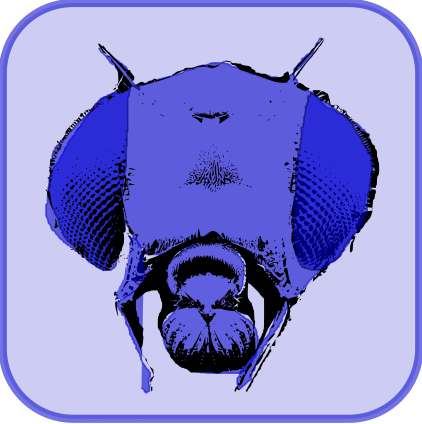
\includegraphics[width=0.06\textwidth,height=\textheight]{figuras/cabezamosca.png} Ejercicios con formato clásico encontrado en libros de genética de poblaciones (de allí que el ícono sea la cabeza de una \emph{Drosophila melanogaster}). Generalmente refieren a \emph{loci} segregando en una población de organismos imaginarios o situaciones similares.\\


\includegraphics[width=0.06\textwidth,height=\textheight]{figuras/agro.png} Ejercicios con particular interés para las agrociencias. Los mismos suelen referir al mejoramiento genético de animales o plantas, o refieren a organismos de especial interés para esta disciplina.\\


\includegraphics[width=0.06\textwidth,height=\textheight]{figuras/cienciabasica.png} Ejercicios inspirados en experimentos de ciencia básica (\emph{i.e.}, biología molecular, genética, bioquímica, microbiología, ecología, etc.).\\


\includegraphics[width=0.06\textwidth,height=\textheight]{figuras/sigma.png} Ejercicios de demostración. Se pide demostrar alguna propiedad matemática a partir de las formulas presentadas en el capítulo. En general, los resultados demostrados ilustran aspectos biológicos interesantes que se desprenden de las bases teóricas desarrolladas en el texto.\\


\includegraphics[width=0.06\textwidth,height=\textheight]{figuras/medicina.png} Ejercicios de particular interés para las áreas biomédicas.

\end{recuadro}

\hfill\break

\part*{Parte I: Genómica}\label{part-parte-i-genuxf3mica}
\addcontentsline{toc}{part}{Parte I: Genómica}

\chapter{Introducción a la Genómica}\label{intro}

El presente capítulo es una somera introducción a la genómica y apenas tiene como cometido el asegurarnos de que algunos conceptos básicos sobre la misma, que usaremos durante el curso, se encuentren disponibles. El foco del mismo es en diferentes metodologías para el estudio de los genomas, muchas de las cuales usaremos en distintos ejemplos y secciones del curso. Poco esfuerzo se hace por explicar las bases de la herencia y la estructura y organización de los genomas eucariotas y procariotas, las cuales se asumen conocidas.

Los organismos en nuestro planeta derivan todos de un organismo ancestral, desconocido, y por lo tanto es de esperar que sus genomas compartan determinadas características. Sin embargo, al mismo tiempo podemos observar una enorme diversidad entre los mismos, por lo que resulta fundamental entender los procesos que llevan a esas diferencias. Dichos procesos operan sobre el componente heredable de los organismos, su material genético. El mismo está compuesto por una secuencia ordenada de nucleótidos, por lo cual es común referirse a este coloquialmente como \emph{secuencia/s} en el ámbito de la genómica y las disciplinas afines. Conocer las secuencias de los genomas de diferentes organismos y compararlas para determinar las diferencias entre estas es, por lo tanto, el primer paso a dar para comprender los procesos que llevaron a dichas diferencias. La secuenciación de genomas es una historia que comenzó en las últimas décadas del siglo pasado y desde ese momento no ha dejado de crecer, en ciertos momentos a velocidad vertiginosa. En particular, la aparición de las denominadas tecnologías de segunda y tercera generación ha permitido pasar de la secuenciación de un genoma por especie a la secuenciación de cientos o miles de individuos de una misma especie. De esta forma, en la acutalidad se está logrando caracterizar mucho mejor la variabilidad biológica existente.

La diversidad existente a nivel de organismos macroscópicos es evidente. El ser humano interacciona con la flora y la fauna desde sus inicios como especie. Entender, preservar e influir sobre esta diversidad biológica es lo que ha permitido en última instancia el desarrollo de las civilizaciones. Resulta intuitivo que enriquecer nuestra comprensión de esta diversidad con aportes desde la genómica pueda resultar valioso. Por otra parte, aunque invisibles los microorganismos juegan un papel relevante en casi todos los ecosistemas a diferentes escalas: desde bosques, praderas, ríos y mares a los ecosistemas internos (\emph{e.g.}, aparato digestivo) y externos (piel) de los organismos. A pesar de su importancia, la diversidad microbiana apenas ha sido explorada, fundamentalmente debido a las dificultades asociadas al cultivo de los microorganismos, muchos de ellos directamente no-cultivables. En este sentido, también la genómica ha jugado un rol destacado en los avances que se han producido en este campo en los últimos años. La \emph{metagenómica}, la \emph{metagenómica funcional} y la \emph{metatranscriptómica} han contribuido a entender la composición de los ecosistemas microbianos, las funciones de los genes involucrados y la regulación de su expresión, respectivamente. Mencionaremos cada una de estas aproximaciones en secciones posteriores de este capítulo.

Aunque a primera vista la informática y la biología puedan parecer áreas de estudio muy alejadas (¿qué se aleja más de la vida que una fría máquina?), veremos que la obtención y procesamiento masivo de datos biológicos han permitido enriquecer de forma importante la perspectiva que tenemos sobre los organismos vivos y la transmisión de información de generación en generación, tanto a nivel individual como poblacional. A lo largo del libro iremos profundizando en esta perspectiva, empleando recursos informáticos para modelar procesos de la genética poblacional y cuantitativa, haciendo un uso enriquecedor de las tecnologías disponibles en la actualidad.\\

\begin{boxobjetivos}
\(\square\) Abordar el fenómeno de la variabilidad genética, discutiendo el uso de métricas que nos permiten cuantificar la misma e introduciendo tecnologías que nos permiten la identificación de variantes genéticas en poblaciones.
\newline

\(\square\) Obtener una perspectiva de las distintas áreas de estudio de la genómica, incluyendo:
- el estudio de la composición nucleotídica de los genomas
- el estudio evolutivo de los organismos
- el análisis de los patrones de expresión génica
\newline

\(\square\) Repasar conceptos básicos de genética y biología molecular, ilustrando en cada caso cómo uso de herramientas estadísticas y computacionales enriquece nuestra perspectiva de los fenómenos biológicos.

\end{boxobjetivos}

\section{Variabilidad genética}\label{variabilidad-genuxe9tica}

Todos los organismos presentan diferencias observables (\emph{fenotípicas}) entre ellos. Muchas de estas son producto del desarrollo en determinados ambientes (específicas para cada individuo), mientras que otras se corresponden a las diferencias en el genoma. Excepto los clones (copias idénticas de un mismo individuo), todos los organismos son de alguna manera diferentes entre sí. Aún entre gemelos es posible postular que la \textbf{\emph{epigenética}}\footnote{Se denomina como epigenético todo cambio heredable que no tiene como base un cambio a nivel de nucleótido en la secuencia de ADN. A modo de ejemplo, cambios en el estado de metilación de un nucleótido pueden influir en el estado de compactación de la cromatina y así en la expresión de algunos genes; esto puede resultar en cambios fenotípicos heredables, aún cuando en ningún momento se haya reemplazado un nucleótido por otro.} puede jugar un rol diferente en su desarrollo. Estas diferencias a nivel genético o genómico son las que nos resultan fundamentales cuando hablamos de mejorar una especie de nuestro interés o en cualquier instancia en la que busquemos seleccionar algunos individuos de una población.

Muchas otras veces estamos más interesados en entender las diferencias entre especies y el rol que juegan las proporciones de individuos de las mismas en la dinámica de un ecosistema. Claramente, la robustez de un ecosistema suele estar asociada al balance de diversas especies, cada una jugando roles diferentes. Pero ese balance no solo depende de la presencia de algún miembro de cada especie, sino de las proporciones que esas especies ocupan en el ecosistema. Tener índices que nos permitan cuantificar y comparar la diversidad existente en diferentes escenarios resulta por lo tanto útil. Tradicionalmente, en ecología se definen tres tipos de medidas de diversidad: la \emph{diversidad alfa}, la \emph{diversidad beta} y la \emph{diversidad gamma}, de acuerdo a la escala del fenómeno estudiado.

Se llama \textbf{\emph{diversidad alfa}} a la que describe la diversidad de especies dentro de una comunidad\footnote{En ecología se define a una \emph{comunidad} como un conjunto de poblaciones de dos o más especies que conviven al mismo tiempo en una misma área geográfica. Un \emph{ecosistema} está compuesto de una comunidad y del entorno abiótico que comprende a la misma. Ambos conceptos son amplios, y pueden referir a unidades ecológicas de tamaños y características diversas.} a una escala pequeña o local. Esta escala es normalmente del tamaño de un ecosistema y es a la que generalmente nos referimos al hablar de una zona.

La \textbf{\emph{diversidad beta}} describe la diversidad de especies entre dos comunidades o ecosistemas. Involucra una escala mayor, ya que incluye ecosistemas (que correspondían a la diversidad alfa) y en general suele haber alguna distinción geográfica o barrera importante entre las comunidades de referencia.

La \textbf{\emph{diversidad gamma}} se refiere a una escala de estudio mucho mayor (\emph{e.g.}, un bioma), donde se compara la diversidad de especies entre muchos ecosistemas.

Aunque la diversidad biológica puede cuantificarse de muchas maneras diferentes, los dos factores principales que se tienen en cuenta para medir la diversidad son la \textbf{\emph{riqueza}} y la \textbf{\emph{uniformidad}}. La riqueza representa el número de tipos (especies) diferentes entre todos los que identificamos en el área de interés. Sin embargo, nuestra intuición nos dice que la uniformidad representa también una parte importante de la diversidad. Es decir, si en un ambiente tenemos 1 individuo de cada una de 4 especies y 996 individuos de una quinta especie, claramente identificaremos una menor diversidad respecto a otro ambiente que tiene 200 individuos de cada una de las especies. En general, la uniformidad compara la similitud del tamaño de la población de cada una de las especies presentes.

Para cada uno de estos tipos de diversidad se han desarrollado índices que permiten obtener estimaciones de su importancia relativa a otros sistemas. Por ejemplo para la diversidad alfa el índice más sencillo de entender es la \emph{entropía de Shannon} (llamada así por el matemático Claude Shannon que la propuso para un problema de transmisión de información), que mide la incertidumbre al asignar la identidad de un individuo elegido al azar de la población. Si le llamamos \(p_i\) a la proporción (frecuencia relativa) de individuos de la especie \(i\), de un total de \(k\) especies identificadas en el ecosistema, entonces el \textbf{\emph{índice de Shannon}} se calcula como

\begin{equationbox}
\begin{equation}
H'=-\sum^k_{i=1} p_i \ln p_i
\label{eq:alphadiver1}
\end{equation}

\end{equationbox}

Es decir, cada frecuencia es multiplicada por su logaritmo y sumada, con el resultado final multiplicado por \(-1\) ya que cualquiera de los logartitmos será menor o igual a cero (porque para todas las especies \(0 \leqslant p_i \leqslant 1\)). En el caso de una sola especie \(\ln p_i=\ln 1=0\), por lo que la diversidad será cero. Cuanto más homogéneo sea el reparto de las especies, mayor será el índice de Shannon. En particular, el máximo del índice de Shannon se dará cuando \(p_i=\frac{N/k}{N}=\frac{1}{k}\ \forall \ i\), en cuyo caso

\[
\begin{split}
H_{max}=-\sum^k_{i=1} \frac{1}{k} \ln \frac{1}{k}=\\
=k\ \frac{1}{k} [\ln 1 -\ln k]=-[0-\ln k] \therefore \\
H_{max}=\ln k
\end{split}
\label{eq:alphadiver1p1}
\]

Es decir, el máximo del índice será el logaritmo del número de especies, lo que ocurre cuando todas las especies tienen el mismo número de integrantes.
Podemos ver entonces que el índice de Shannon no sólo nos permite comparar la diversidad biológica de forma cuantitativa, sino que además nos permite predecir bajo qué condiciones ésta se maximiza. Lo que es más, esta predicción se corresponde con nuestra intuición de que una mayor diversidad debe reflejar un reparto más equitativo de los individuos para las diferentes especies (concepto de uniformidad mencionado anteriormente).

Resulta claro que los valores que se pueden obtener para el índice de Shannon dependerán del número de especies presentes (\(k\)) en el ecosistema estudiado.
En este sentido, resulta útil un índice relacionado directamente al índice de Shannon es el propuesto por Pielou (\citeproc{ref-Pielou1969}{1969}), que estandariza el índice de Shannon por la riqueza, lo que lo deja como un índice de uniformidad (``\emph{evenness}'', en inglés) que se calcular como

\begin{equation}
E=\frac{H'}{H_{max}}=\frac{H'}{\ln k}
\label{eq:alphadiver1p2}
\end{equation}

Así, es posible tener una noción más clara respecto a la diversidad alfa presente en el ecosistema estudiado: cuanto más se acerca este índice \(E\) a 1, más cerca se estará del máximo teórico según el índice de Shannon.

Otro índice popular es el \textbf{\emph{índice de Simpson}}. El índice de Simpson (\(D\)) mide la probabilidad de que dos individuos seleccionados al azar de una muestra pertenezcan a la misma especie o categoría. Es decir, si \(n_i\) representa el número de individuos de la especie o categoría \(i\) y \(N\) el número total de individuos, es decir \(N=\sum_i n_i\), entonces

\begin{equationbox}
\begin{equation}
D=\sum^k_{i=1} \frac{n_i(n_i-1)}{N(N-1)}
\label{eq:alphadiver2}
\end{equation}

\end{equationbox}

La intuición de este índice es que si los individuos se concentran en pocos tipos diferentes el valor de \(D\) será más alto, es decir lo contrario a lo que esperaríamos para un índice de diversidad. De hecho, con este índice 0 representa una diversidad infinita y 1, ninguna diversidad. Es decir, cuanto mayor sea el valor de \(D\), menor será la diversidad. Para superar este problema, se suele restar a 1 el valor de \(D\), es decir se reporta \(1-D\). Otra alternativa es reportar el recíproco de \(D\), es decir \(1/D\). Cuando el número de individuos es muy grande, entonces en general \(\frac{n_i -1}{N-1} \to \frac{n_i}{N}\), por lo que

\[
\begin{split}
D=\sum^k_{i=1} \frac{n_i(n_i-1)}{N(N-1)}=\sum^k_{i=1} \frac{n_i}{N}\frac{(n_i-1)}{(N-1)} \approx \sum^k_{i=1} \frac{n_i}{N}\frac{(n_i)}{(N)} \therefore \\
D \approx \sum^k_{i=1} \frac{n^2_i}{N^2}
\end{split}
\label{eq:alphadiver2p1}
\]

Notemos que hasta el momento no se han tenido en cuenta posibles errores al momento de determinar el número de especies \emph{k} presentes en una muestra (\emph{e.g.} por falta de muestreo de organismos de una especie presente en el ecosistema en números muy bajos).

El \textbf{\emph{índice de cobertura de Good}} es usado a veces como estimador de diversidad alfa y se calcula mediante la siguiente ecuación:

\begin{equation}
C=1-\frac{F_1}{N}
\label{eq:alphadiver3}
\end{equation}

donde \(F_1\) es el número de \textbf{OTUs} (``\emph{Operational Taxonomic Units}''; Unidades Taxonómicas Operacionales, en inglés) en la muestra con un solo representante. \textbf{OTU} es una forma de expresar una unidad taxónomica particular a un nivel de la taxonomía determinado. Por ejemplo, en algunos casos las \textbf{OTUs} pueden representar especies, pero otras veces representan niveles más altos o más bajos de la taxonomía (de ahí el término ``\emph{operacional}''). La idea del índice es capturar de alguna manera la probabilidad de perder \textbf{OTUs} debido a un tema de muestreo. Es decir, aquellas \textbf{OTUs} que no fueron secuenciadas pero que se encontraban presentes, las cuales se hallarían de haberse realizado muestreos con tamaños muestrales mucho mayores.

La diversidad juega un papel fundamental en la resiliencia de los sistemas, tanto la diversidad entre especies como dentro de especies. Por ejemplo, la pérdida de diversidad asociada a la revolución verde entre la década del 60 y del 80 del siglo XX representa una pérdida irrecuperable de patrimonio genético desarrollado durante miles y millones de años. Lamentablemente, es poco probable que la biotecnología pueda recuperar en breve lo que la naturaleza desarrolló durante millones de años, por lo que resulta trascendental pensar en conservar la diversidad en nuestro planeta.

\subsection*{Ejemplo 1.1}\label{ejemplo-1.1}
\addcontentsline{toc}{subsection}{Ejemplo 1.1}

Luego de un muestreo realizado a partir de \textbf{\emph{metagenómica}} en dos ambientes diferentes, la distribución de especies (\textbf{\emph{OTUs}}) en los mismos es la siguiente:

\begin{table}
\centering
\begin{tabular}[t]{lll}
\toprule
Especie & Ambiente.1 & Ambiente.2\\
\midrule
\cellcolor{gray!10}{OTU 1} & \cellcolor{gray!10}{$60$} & \cellcolor{gray!10}{$1$}\\
OTU 2 & $150$ & $1$\\
\cellcolor{gray!10}{OTU 3} & \cellcolor{gray!10}{$0$} & \cellcolor{gray!10}{$297$}\\
OTU 4 & $390$ & $1$\\
\cellcolor{gray!10}{OTU 5} & \cellcolor{gray!10}{$400$} & \cellcolor{gray!10}{$700$}\\
\addlinespace
Total & $1000$ & $1000$\\
\bottomrule
\end{tabular}
\end{table}

Calcular los difentes índices para los dos ambientes y discutir los resultados.

Como el total de ``individuos'' (\textbf{\emph{reads}}) obtenidos en ambas muestras es \(1000\), alcanza con dividir entre ese número para tener la frecuencia relativa. Por lo tanto, utilizando la ecuación \eqref{eq:alphadiver1} el índice de Shannon para el primer ambiente es igual a

\[
\begin{split}
H'*1=-\sum^k*{i=1} p_i \ln p_i =\\
=-[0,06 \times \ln 0,06 + 0,15 \times \ln 0,15 + 0,39 \times \ln 0,39 +\\
- 0,4 \times \ln 0,4] \therefore \\
H'_1=1,1871
\end{split}
\]

mientras que para el segundo ambiente el mismo es

\[
\begin{split}
H'*2=-\sum^k*{i=1} p_i \ln p_i =\\
=-[0,001 \times \ln 0,001 + 0,001 \times \ln 0,001 + 0,297 \times \ln 0,297 +\\
+0,001 \times \ln 0,001 + 0,7 \times \ln 0,7] \therefore \\
H'_2=0,63096
\end{split}
\]

Notar que en el \textbf{Ambiente 1} no se encontró la especie \textbf{OTU 3}, por lo que no se incluye en los cálculos (de hecho \(\ln 0=-\infty\)). De acuerdo con esto, según el \textbf{índice de Shannon} el \textbf{Ambiente 1} es más diverso que el \textbf{Ambiente 2}. Para medir la uniformidad utilizando el índice propuesto por Pielou (1969), primero tenemos que calcular el máximo posible para el índice de Shannon, que a partir de la ecuación \eqref{eq:alphadiver1p1} sabemos que es igual al logaritmo del número de \textbf{OTUs}, es decir \(H_{max_1}=\ln k=\ln 4=1,3863\) y \(H_{max_2}=\ln k=\ln 5=1,6094\). Por lo tanto, aplicando la ecuación \eqref{eq:alphadiver1p2}, tenemos que el índice de uniformidad para los dos ambientes será

\[
\begin{split}
E_1=\frac{H'*1}{H*{max_1}}=\frac{1,1871}{1,3863}= 0,8563 \\
E_2=\frac{H'*2}{H*{max_2}}=\frac{0,63096}{1,6094}= 0,3920
\end{split}
\]

lo que habla de una uniformidad mucho menor en el \textbf{Ambiente 2}.

Para el índice de Simpson vamos a utilizar la ecuación \eqref{eq:alphadiver2}, por lo que para el \textbf{Ambiente 1} el mismo será

\[
\begin{split}
D_1=\sum^k_{i=1} \frac{n_i(n_i-1)}{N(N-1)}=\\
=\left[\frac{60(59)+150(149)+390(389)+400(399)}{1000 \times 999}\right]=0,3375
\end{split}
\]

mientras que para el \textbf{Ambiente 2} su valor será

\[
\begin{split}
D_2=\sum^k_{i=1} \frac{n_i(n_i-1)}{N(N-1)}=\\
=\left[\frac{1(0)+1(0)+297(296)+1(0)+700(699)}{1000 \times 999}\right]=0,5778
\end{split}
\]

Si utilizamos el criterio de reportar \(1-D\), entonces \(1-D_1=1-0,6625\), mientras que \(1-D_2=1-0,4222\). Si utilizamos el criterio del recíproco, entonces \(1/D_1=2,9626\) y \(1/D_2=1,7307\), por lo que se aprecia claramente que la diversidad en el \textbf{Ambiente 1} es mayor que la del \textbf{Ambiente 2} de acuerdo a este índice.

Finalmente, de acuerdo a la ecuación \eqref{eq:alphadiver3}, teniendo en cuenta que en el primer ambiente no hay ningún OTU con un único representante mientras que en el segundo hay 3, el \textbf{índice de cobertura de Good} para los dos ambientes sería

\[
\begin{split}
C_1=1-\frac{0}{1000}=1 \\
C_2=1-\frac{3}{1000}=0,997
\end{split}
\]

\begin{graybox}

\begin{itemize}
\item
  Tradicionalmente, en ecología se definen tres tipos de medidas de diversidad de acuerdo a la escala del fenómeno estudiado:

  \begin{itemize}
  \tightlist
  \item
    Se llama \textbf{\emph{diversidad alfa}} a la que describe la diversidad de especies dentro de una comunidad a una escala pequeña o local. Esta escala es normalmente del tamaño de un ecosistema y es a la que generalmente nos referimos al hablar de una zona.
  \item
    La \textbf{\emph{diversidad beta}} describe la diversidad de especies entre dos comunidades o ecosistemas. Involucra una escala mayor, ya que incluye ecosistemas (que correspondían a la diversidad alfa) y en general suele haber alguna distinción geográfica o barrera importante entre las comunidades de referencia.
  \item
    La \textbf{\emph{diversidad gamma}} se refiere a una escala de estudio mucho mayor (\emph{e.g.},un bioma), donde se compara la diversidad de especies entre muchos ecosistemas.
  \end{itemize}
\item
  Aunque la diversidad biológica puede cuantificarse de muchas maneras diferentes, los dos factores principales que se tienen en cuenta para medir la diversidad son la \textbf{\emph{riqueza} y la \emph{uniformidad}}. La \textbf{\emph{riqueza}} representa el número de tipos (especies) diferentes entre todos los que identificamos en el área de interés, mientras que la \textbf{\emph{uniformidad}} compara la similitud del tamaño de la población de cada una de las especies presentes.
\item
  Para la diversidad alfa, el índice más sencillo de entender es la \emph{entropía de Shannon}, que mide la incertidumbre al asignar la identidad de un individuo elegido al azar de la población. Si le llamamos \(p_i\) a la proporción (frecuencia relativa) de individuos de la especie \(i\), de un total de \(k\) especies identificadas en el ecosistema, entonces el \textbf{\emph{índice de Shannon}} se calcula como: \(H'=-\sum^k_{i=1} p_i \ln p_i\).
  Cuanto más homogéneo sea el reparto de las especies, mayor será el índice de Shannon. El máximo del mismo será cuando todas las especies tienen el mismo número de integrantes.
\item
  El \textbf{\emph{índice de Simpson} (\(D\))} mide la probabilidad de que dos individuos seleccionados al azar de una muestra pertenezcan a la misma especie o categoría. Es decir, si \(n_i\) representa el número de individuos de la especie o categoría \(i\) y \(N\) el número total de individuos (\emph{i.e.}, \(N=\sum_i n_i\)), entonces \(D=\sum^k_{i=1} \frac{n_i(n_i-1)}{N(N-1)}\). La intuición de este índice es que si los individuos se concentran en pocos tipos diferentes el valor de \(D\) será más alto, al contrario de lo que esperaríamos para un índice de diversidad. Para superar este problema, se suele restar a 1 el valor de \(D\) (se reporta \(1-D\)).
\end{itemize}

\end{graybox}

\subsection{Detectando la variabilidad: diferentes técnicas}\label{detectando-la-variabilidad-diferentes-tuxe9cnicas}

En las últimas décadas han ganado una enorme relevancia un conjunto de disciplinas con base en avances tecnológicos que permiten la obtención masiva de información biológica global para una condición dada. Esto se logra a través de la automatización de diversos protocolos de bioquímica y biología molecular, tales como la secuenciación de nucleótidos o péptidos provenientes de una muestra biológica. Estas disciplinas son identificables por la utilización del sufijo ``\emph{-ómica}'' en su nombre. La \emph{genómica} es una de estas disciplinas, focalizándose en el estudio del genoma de diferentes organismos a través de las tecnologías de secuenciación masiva. Existen también la \emph{transcriptomica} (estudio global de los transcriptos expresados por un organismo o conjunto de células), la \emph{proteómica} (estudio de las proteńas expresadas en una condición dada) o la \emph{metabolómica} (estudio del perfil metabólico), entre otros. Este enfoque de análisis también se puede aplicar para estudiar varios organismos a la vez (\emph{e.g.} al tomarse muestras ambientales), surgiendo así un subconjunto de discplinas ``meta-''. A modo de ejemplo, la metagenómica se encarga del ensamblado y estudio de genomas microbianos en muestras provenientes de diferentes lugares. En la Sección \hyperref[metagenomica-y-metatranscriptomica]{Metagenómica y metatranscriptómica} se detalla un esquema típico de trabajo en metagenómica. Como es de esperar, estas técnicas de obtención masiva de datos han impactado de forma notable nuestro entendimiento de la variabilidad genética entre organismos.

Para entender la variabilidad genética es necesario determinar algún marcador genético cuyas variantes podamos detectar en muchos individuos (\emph{e.v.}, obteniendo las secuencias para el marcador en esta muestra). Un ejemplo de estudios iniciales de diversidad genética es la utilización de grupos sanguíneos, el cual veremos en el próximo capítulo. Hasta hace algunos años la búsqueda de marcadores fiables de diversidad genética representaba un enorme desafío, y se desarrollaron una plétora de métodos para obtener marcadores moleculares de diversidad. Tanto el trabajo como los costos eran enormes, lo que dificultaba el desarrollo de estudios a gran escala en este sentido. Afortunadamente, a fines del siglo XX las técnicas de secuenciación masiva habían avanzado lo suficiente como para incluir centenas de individuos en los estudios. Más aún, el desarrollo de técnicas como los \textbf{\emph{microarrays}} posibilitaron la automatización de muchos análisis (en especial los de expresión), pero también resultaron fundamentales a la hora de abaratar los costos para estudios masivos de diversidad.

Los \textbf{\emph{microarrays}} son un arreglo de \textbf{sondas moleculares} colocadas en una placa. Originalmente contenían apenas unas decenas de sondas; la robotización y la aplicación de tecnologías que se usan en la fabricación de semiconductores permitieron alcanzar densidades del orden del millón de sondas por \emph{array} (placa). Una sonda molecular, en este caso, es una secuencia específica para un gen (o una región de un gen) y que es, idealmente, única en el genoma de referencia. Esta sonda se encuentra fija en la placa, y la hibridación del \textbf{ADN} o el \textbf{ADN copia} (en los estudios de transcriptómica) de un individuo es acoplada a algún tipo de señal (\emph{e.g.}, emisión de luz en determinada frecuencia al ser iluminada por un \textbf{láser}). La presencia de señal permite se asocia, por lo tanto, a la presencia del ADN de interés en la muestra proveniente del individuo.

Esta tecnología permite, por ejemplo, identificar si la secuencia presente en el organismo es de un tipo u otro en el caso de los \textbf{SNPs} (polimorfismos de un solo nucleótido). En el caso de las especies diploides, es posible identificar el genotipo para un organismo. Para conocer la diversidad del genoma humano es usual utilizar chips de densidad media (10-60K de SNPs) o de alta densidad (hasta un millón de SNPs). En especies de interés comercial existen diferentes tipos de alternativas, desde \emph{arrays} de baja densidad (apenas unos pocos miles de SNPs), media, hasta los de alta densidad, como el \textbf{BovineHD} que comprende más de 777 mil SNPs, compatible con todas las razas bovinas lecheras o de carne.

A pesar del enorme éxito de los \emph{microarrays} para estudiar la diversidad genética en diversas poblaciones de diferentes especies, los mismos padecen de un problema fundamental: para crear una sonda para medir variabilidad hay que conocer las secuencias de regiones que contengan variabilidad. Es decir, para estudiar la variabilidad mediante esta técnica hay que tener alguna información previa de qué regiones son variables. Esto se debe a que la suma de los tamaños de las sondas son extremadamente pequeños en relación al largo total de los genomas. Por ejemplo, en genoma humano un chip de alta densidad cubre 1 millón de posiciones de las más de 3.000 millones que tiene el genoma (\textasciitilde0.0003\%). Para elegir bien ese millón de posiciones hay que tener muy buena información previa: si se eligen posiciones que casi no varíen en la población, se obtendrá muy poca información sobre la variabilidad genética en las poblaciones estudiadas. Además, otro problema derivado de los \emph{microarrays} y de este sesgo en los marcadores a incluir es que luego de diseñado el \emph{array} solo va a captar variabilidad en las posiciones del genoma para el que fue diseñado. Si una nueva población aparece con variabilidad importante en otras regiones, el \emph{array} no va a ser capaz de detectarlo. Por ejemplo, en genoma humano, hasta hace poco tiempo los \emph{arrays} poseían un importante sesgo ``eurocéntrico'', porque la mayor parte de la información previa venía de Europa. Esto dejaba fuera de los mismos sitios de alta variabilidad en poblaciones asiáticas o amerindias, por ejemplo. Estudios que utilizaran dichos \emph{arrays} terminarían determinando que estas poblaciones tenían menos variabilidad genética que la real.

Afortunadamente, las \textbf{tecnologías de secuenciación masiva} que se desarrollaron a comienzo del siglo XXI cambiaron definitivamente el panorama, ya que permiten obtener las secuencias de decenas o cientos de individuos a precio y tiempos razonables. Como referencia, el esfuerzo global para obtener la secuencia del primer genoma humano llevó más de 10 años a decenas de laboratorios repartidos en el mundo, y costó más de 3.000 millones de dólares. Actualmente, un genoma humano tarda en secuenciarse menos de una semana (el record mundial, establecido recientemente, es de 5 horas y 2 minutos) y cuesta en promedio unos mil dólares (sin incluir los costos del análisis posterior). Más aún, si bien las tecnologías de segunda generación (\textbf{Roche 454}, \textbf{Illumina} y \textbf{SOLiD}) tuvieron un éxito enorme, la flexibilidad de las mismas era algo limitada y en particular era muy difícil reducir los tiempos de secuenciación, además de tener ciertos sesgos específicos en los resultados. En la segunda década de este siglo comenzaron a aparecer y consolidarse otras nuevas tecnologías, que se dieron en llamar de tercera generación y que incluyen los secuenciadores \textbf{IonTorrent}, los de \textbf{Oxford Nanopore Technologies} y los \textbf{PacBio}. En conjunto, estas tecnologías, sumadas a \textbf{Illumina} que es la única de las de segunda generación que sobrevive con mucho éxito, permiten tener una flexibilidad enorme en tamaños y costos de equipamientos y reactivos, en sesgos y distribución de errores, así como en la velocidad de secuenciación.

\subsection{Metagenómica y metatranscriptómica}\label{metagenomica-y-metatranscriptomica}

En muchos casos nos interesa determinar la estructura de alguna comunidad biológica y estudiar su evolución en el tiempo, o simplemente comparar esa estructura en diferentes condiciones. Por ejemplo, la microbiota ruminal es fundamental para los procesos que determinan la degradación de la materia orgánica que el animal recibe, estando asociada también a qué productos de esta degradación recibirá el animal y en qué proporciones. ¿Qué variables afectan más la composición de la microbiota? ¿El pH ruminal? ¿El porcentaje de materia seca? ¿La proporción de fibra? En el plano de la salud, ¿qué microorganismos se encuentran presentes en la ubre sana y qué microorganismos en la glándula de un animal con mastitis? ¿La infección es a causa de un microorganismo dominante o el patógeno no precisa ser el que domine el ecosistema ruminal? ¿El rol del patógeno es directo sobre la salud del animal o su rol se limita a desestabilizar la ecología de la glándula?

Para poder responder a cualquiera de estas preguntas es necesario poder caracterizar la comunidad microbiana presente. A diferencia de lo que ocurre con especies de plantas, hongos y animales que generalmente podemos percibir y contar a simple vista, con los microorganismos nos ocurre que necesitamos identificarlos de formas más indirectas. Si bien usando el microscopio (con algo de suerte) podríamos ser capaces de reconocer el género de algunas bacterias presentes en una muestra, difícilmente seamos capaces de reconocer a la mayoría. Seríamos mucho menos capaces de reconocer las especies y cepas de estas bacterias, y muchísimo menos capaces de cuantificar la proporción de cada grupo bacteriano. Haciendo un paralelismo, para entender la comunidad vegetal de un bosque no alcanza con determinar la presencia de al menos un ejemplar de una especie: es fundamental entender la proporción que dicha especie ocupa en el ecosistema.

Como ya mencionamos, el hecho de que todos los organismos en nuestro planeta ``desciendan'' del mismo organismo ancestral, a veces conocido como \textbf{LUCA} (``\emph{Last Unknown Common Ancestor}'', en inglés), nos sugiere que sería de esperar encontrar ciertas regularidades en la información genética de los mismos. Es decir, diferentes formas de vida son el producto de modificaciones a formas de vida preexistentes, al menos hasta llegar a \textbf{LUCA}, por lo que de alguna manera todos los seres vivos comparten ciertas características. Las diferencias entre especies, como sabemos, se corresponden en gran medida a cambios en el genoma de los mismos, tanto a nivel de mutaciones puntuales como de inserciones y deleciones, duplicaciones de regiones del genoma o aún re-arreglos cromosómicos. La clave para identificar especies es ubicar secuencias lo suficientemente conservadas como para que deban encontrarse en todos los organismos de interés, pero al mismo tiempo con suficientes cambios entre especies como para poder identificarlas en forma unívoca.

Dentro de las secuencias con estas características, la maquinaria vinculada a la traducción de la información es ciertamente privilegiada ya que constituye un elemento clave para cualquier forma de vida: la capacidad de traducir la información genética en los efectores, que suelen ser la proteínas. La traducción de la información implica una maquinaria tan compleja que resulta completamente implausible su surgimiento de forma independiente en diferentes linajes de la vida, más aún dado que cualquier especie ya hubiese precisado de una para existir. Además, debido a su enorme complejidad se trata de una maquinaria muy ajustada y donde es posible introducir muy pocas variaciones sin que la maquinaria deje de funcionar completamente, en particular porque el \textbf{\emph{fitness}}\footnote{Diferentes individuos tenderán a reproducirse con mayor o menor éxito debido a una variedad de factores tales como la capacidad de sobrevida en un entorno dado o la fecundidad, entre otros. En la teoría evolutiva, este concepto se ve representado por el término \emph{fitness}, que refiere a la contribución reproductiva de un individuo a su próxima generación. Así, diremos que individuos con un mayor \emph{fitness} tienden a dejar mayor descendencia en la próxima generación. Algunos autores hacen referencia al \emph{fitness} de un individuo, mientras que otros refieren al \emph{fitness} de un genotipo particular o incluso de un alelo.} de los organismos tiene, en muchos casos, una vinculación directa con la tasa de producción de las proteínas. Un caso de particular importancia es el \textbf{ARN ribosomal} (\textbf{ARNr}). Este tipo de marcador molecular está constituido por una serie de moléculas de \textbf{ARN} que dependen de su estructura espacial para poder cumplir su rol. Esto incluye apareamientos Watson-Crick entre regiones complementarias, pero también bases modificadas post-transcripcionalmente para asegurar la estabilidad de la molécula y la fidelidad de la traducción.

En procariotas, el \textbf{ARNr 16S} es una molécula usada en forma extensiva para identificar el genero y especie de los organismos. De hecho, la propuesta para un sistema de clasificación de la vida de Woese, Kandler, and Wheelis (\citeproc{ref-WoeseKandlerWheelis1990}{1990}), representada en la Figura \ref{fig:arbolvida}, se basa en las diferencias observadas en la molécula de \textbf{16S} y su equivalente en eucariotas, el \textbf{ARNr 18S}. De acuerdo con esta forma de organizar las diferentes especies, existen tres grandes dominios de la vida: \emph{Bacteria}, \emph{Archaea} y \emph{Eukarya}.\footnote{Interesantemente, la metagenómica ha permitido el descubrimiento reciente de una diversidad arqueana antes desconocidas, lo cual ha llevado a una fuerte controversia en esta área de la filogenética contemporánea. En particular, el descubrimiento en 2015 de un filo arqueano denominado \emph{Asgard} y el análisis en conjunto de diferentes marcadores moleculares ha aportado evidencia congruente con una ``\emph{hipótesis de dos dominios}'' para el árbol de la vida. Según esta hipótesis el dominio Eukarya sería en realidad un subgrupo del dominio Arquea, fuertemente emparentado con el filo Asgard. Más allá de qué hipótesis posea mayor respaldo, esta controversia ilustra hasta qué punto nuevas evidencias provenientes de la genómica y la metagenómica aportan a debates de primer nivel en la teoría biológica; otros ejemplos de relevancia teórica y práctica son mencionados más adelante en esta misma sección.}. Es importante notar que a diferencia de la taxonomía basada en similitud morfológica, la clasificación propuesta por Woese, Kandler, and Wheelis (\citeproc{ref-WoeseKandlerWheelis1990}{1990}) se basa en similitud en las secuencias genómicas, donde de acuerdo a determinados modelos se pueden asignar relaciones de proximidad y distancia entre secuencias pertenecientes a diferentes organismos. En particular, la reconstrucción filogenética se realiza generalmente a partir de secuencias de genes \emph{ortólogos}\footnote{En teoría evolutiva se dice que dos caracteres son \emph{ortólogos} si derivan de un único ancestro común a dos especies. A modo de ejemplo, los genes codificantes para mioglobina de humano y chimpancé son ortólogos, ya que se infiere que el ancestro común a ambas especies poseía una unica copia para este gen; una vez se dió el evento de especiación, pasó a existir una copia para cada especie.}, en este caso el \textbf{ARN ribosomal 16S}, por ejemplo. Si bien desde el punto de vista morfológico los miembros del dominio \textbf{Archaea} no son, aparentemente, muy distintos de los miembros de \textbf{Bacteria}, desde el punto de vista evolutivo poseen grandes diferencias que los hacen acreedores de su propio dominio.



\begin{figure}[H]

{\centering 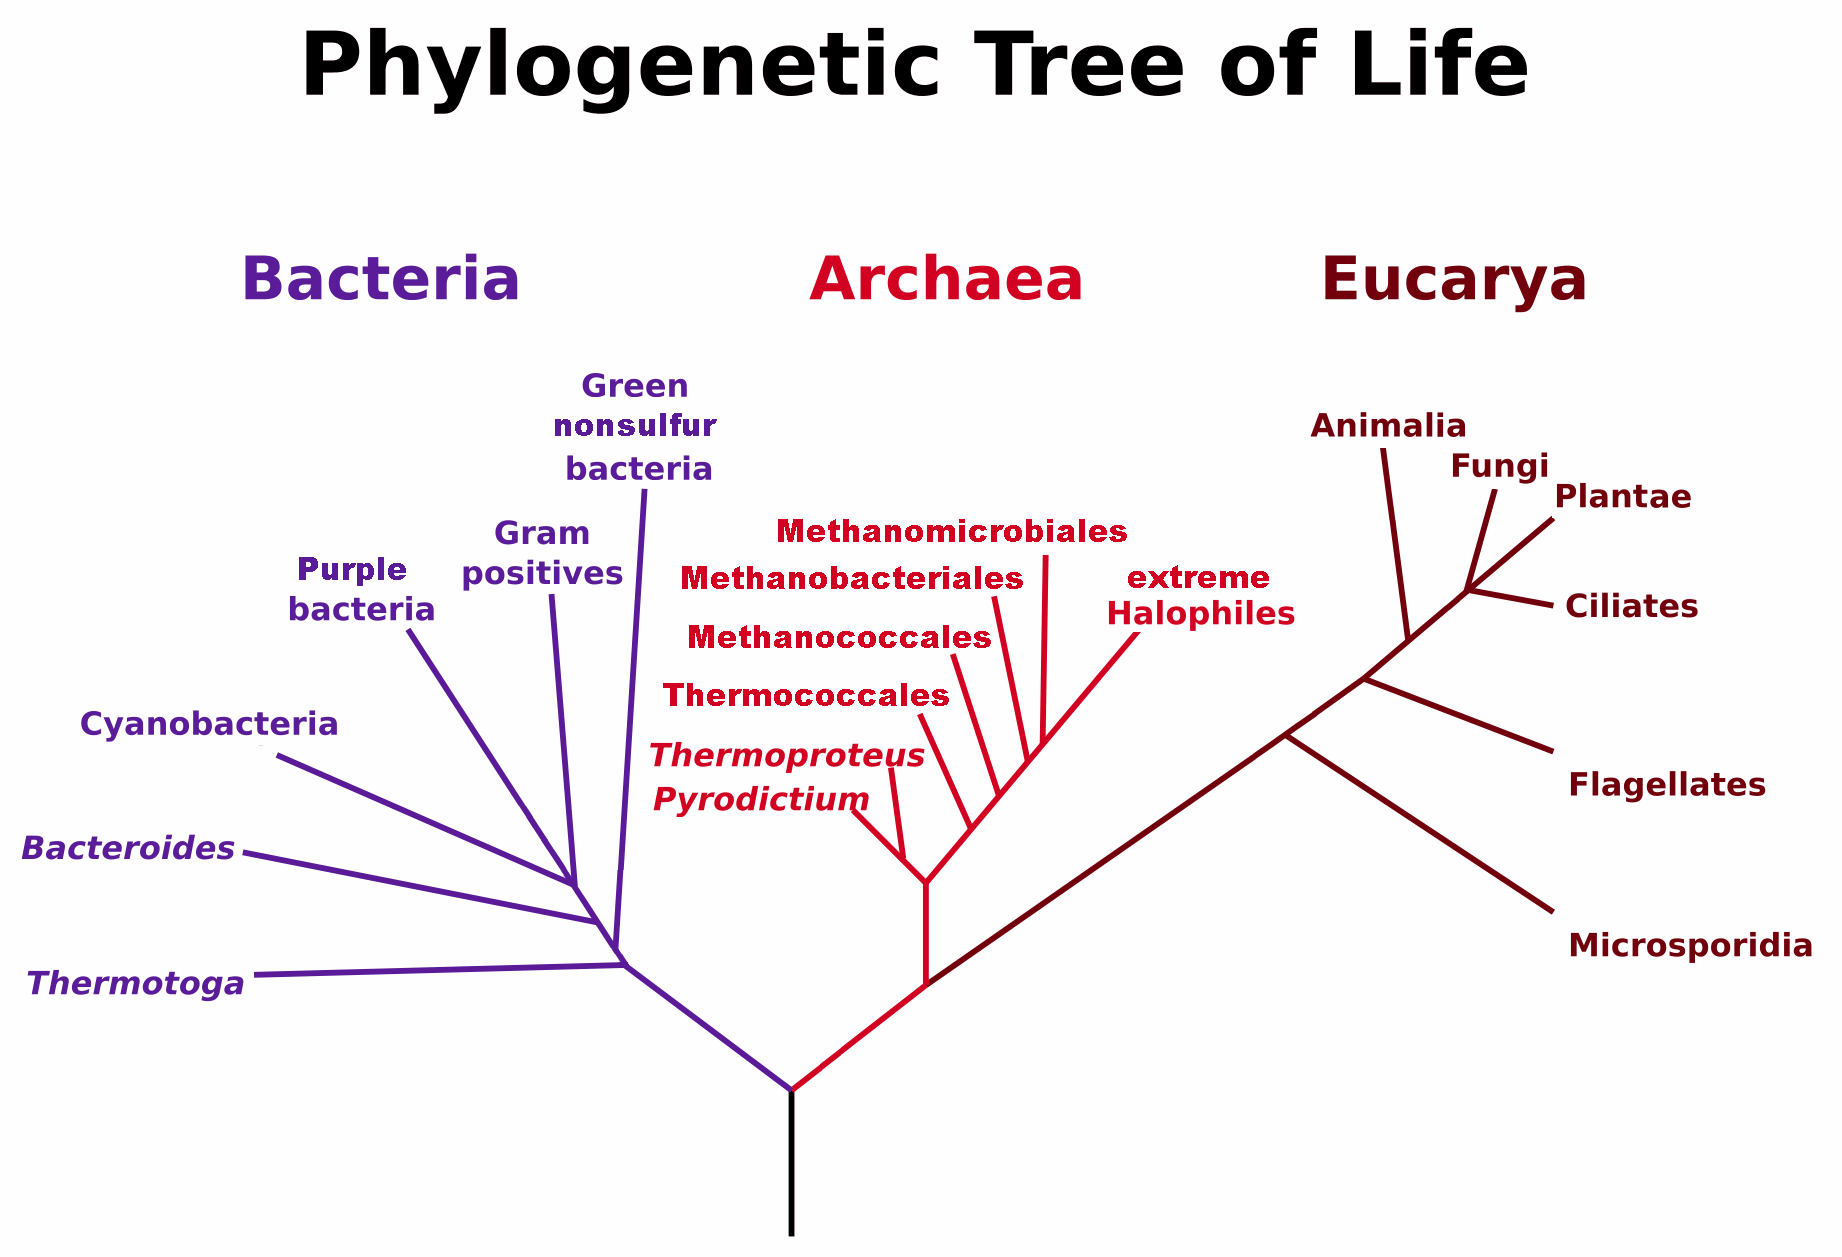
\includegraphics[width=0.7\linewidth]{figuras/PhylogeneticTreeWoese1990} 

}

\caption{Árbol filogenético de los 3 dominios biológicos, \emph{Bacteria}, \emph{Archaea} y \emph{Eukarya}. Con una barra vertical se representa la existencia de \textbf{LUCA}, el último ancestro común, desconocido. (Por Maulucioni - Trabajo Propio, CC BY-SA 3.0, \url{https://commons.wikimedia.org/w/index.php?curid=24740337}).}\label{fig:arbolvida}
\end{figure}

Las técnicas de secuenciación masiva implicaron un salto enorme para la caracterízación de poblaciones microbianas, ya que permiten la secuenciación de miles y hasta millones de fragmentos de secuencias en muy poco tiempo y en forma paralela. La idea más básica consiste en secuenciar una determinada secuencia o región que se encuentre en todos los organismos de interés y que presente suficiente variabilidad, como es el caso del \textbf{ARNr 16S}. Esquemáticamente, los pasos serían los siguientes:

\begin{recuadro}

\begin{enumerate}
\def\labelenumi{\arabic{enumi}.}
\tightlist
\item
  Determinar el grupo de organismos de interés, así como la molécula y región a secuenciar. Las regiones hipervariables \textbf{V3} y \textbf{V4} del \textbf{ARNr 16S} son buenas candidatas iniciales para procariotas. El gen tiene una longitud aproximada de 1.500 pb y contiene nueve regiones variables intercaladas entre regiones conservadas. Qué región del ARNr 16S secuenciar es un área de debate, y la misma puede variar dependiendo de cosas como los objetivos experimentales, el diseño y el tipo de muestra, aunque las regiones \textbf{V3} y \textbf{V4} son ampliamente utilizadas.
\item
  Extraer los ácidos nucleicos de interés y amplificar por PCR las regiones de interés. Los protocolos permiten en general utilizar ``\emph{barcodes}'', que son secuencias específicas que se agregan a las secuencias (un ``\emph{barcode}'' para cada muestra), lo que permite correr en paralelo hasta 96 muestras en una misma ``corrida'' del secuenciador.
\item
  Secuenciar las muestras preparadas de acuerdo al protocolo. Existen diferentes tecnologías y en distintos tamaños, lo que permite secuenciar desde unas poquitas muestras hasta centenas de ellas a un costo razonable y en tiempos razonables. Las distintas tecnologías poseen problemas diferentes, pero en general no introducen sesgos importantes en la composición estimada de la muestra.
\item
  Control de calidad y limpieza de las secuencias obtenidas. Es una serie de procesos a nivel bioinformático que tienen por objetivo eliminar las secuencias de los adaptadores que se agregaron durante la preparación de las bibliotecas, separar las secuencias de acuerdo al correspondiente ``\emph{barcode}'' y calcular una serie de parámetros que indican la calidad de la corrida y de cada una de las muestras.
\item
  Agrupamiento de secuencias y mapeo contra bases de datos con secuencias identificadas. Se trata del corazón de la idea y consiste en que cada secuencia o fragmento producido durante la secuenciación debe tener uno idéntico depositado en una base de datos con secuencias de organismos. Hay diferentes estrategias respecto a cómo agrupar los fragmentos antes de ``mapearlos'' contra las bases de datos y diferentes bases de datos de organismos, pero esto ya es materia específica de la bioinformática.
\item
  Una vez mapeadas las secuencias obtenidas, es decir que a cada una le asignamos un \textbf{taxón} determinado (puede llegar a ser una especie, aunque a veces la identificación queda a un nivel más alto, por ejemplo género), entonces alcanza con contar cuántas veces aparece cada organismo en una muestra (es decir, cuántos fragmentos secuenciados mapean al mismo taxón). Esto nos permite organizar la información en una tabla que puede tener las muestras en filas y los taxa en las columnas.
\item
  Análisis de la tabla de conteos. Por lo general la tabla generada de conteos tiene diferencias importantes en el número de secuencias obtenidas por muestra ya que no se obtiene la misma cantidad de ácidos nucléicos en cada muestra a pesar de los esfuerzos. Para la parte de exploración suelen usarse análisis exploratorios multivariados, como el \textbf{escalado multidimensional} (MDS), una técnica con cierta relación al PCA en su versión más clásica (que se conoce como \textbf{Principal Coordinates Analysis}, PCoA). La idea es reducir la dimensionalidad del problema de tal forma que se pueda representar en pocas dimensiones con poca pérdida de información. En el mejor de los casos, después es posible correlacionar directamente las posiciones de la muestras en las principales dimensiones con factores externos, tales como el pH, la temperatura, ubicación geográfica o cualquier otro factor que sea relevante. En la Figura \ref{fig:mdslepto} se observa la representación gráfica de los dos primeros ejes en un análisis MDS realizado como control de calidad en un experimento de \textbf{transcriptómica RNA-seq} con \textbf{\emph{Leptospira biflexa}}. Se observa que las muestras se agrupan de acuerdo a la condición biológica y que los dos factores relevantes desde el punto de vista biológico (fase de crecimiento y tiempo) son las que separan las muestras entre sí.
\end{enumerate}

\end{recuadro}



\begin{figure}[H]

{\centering 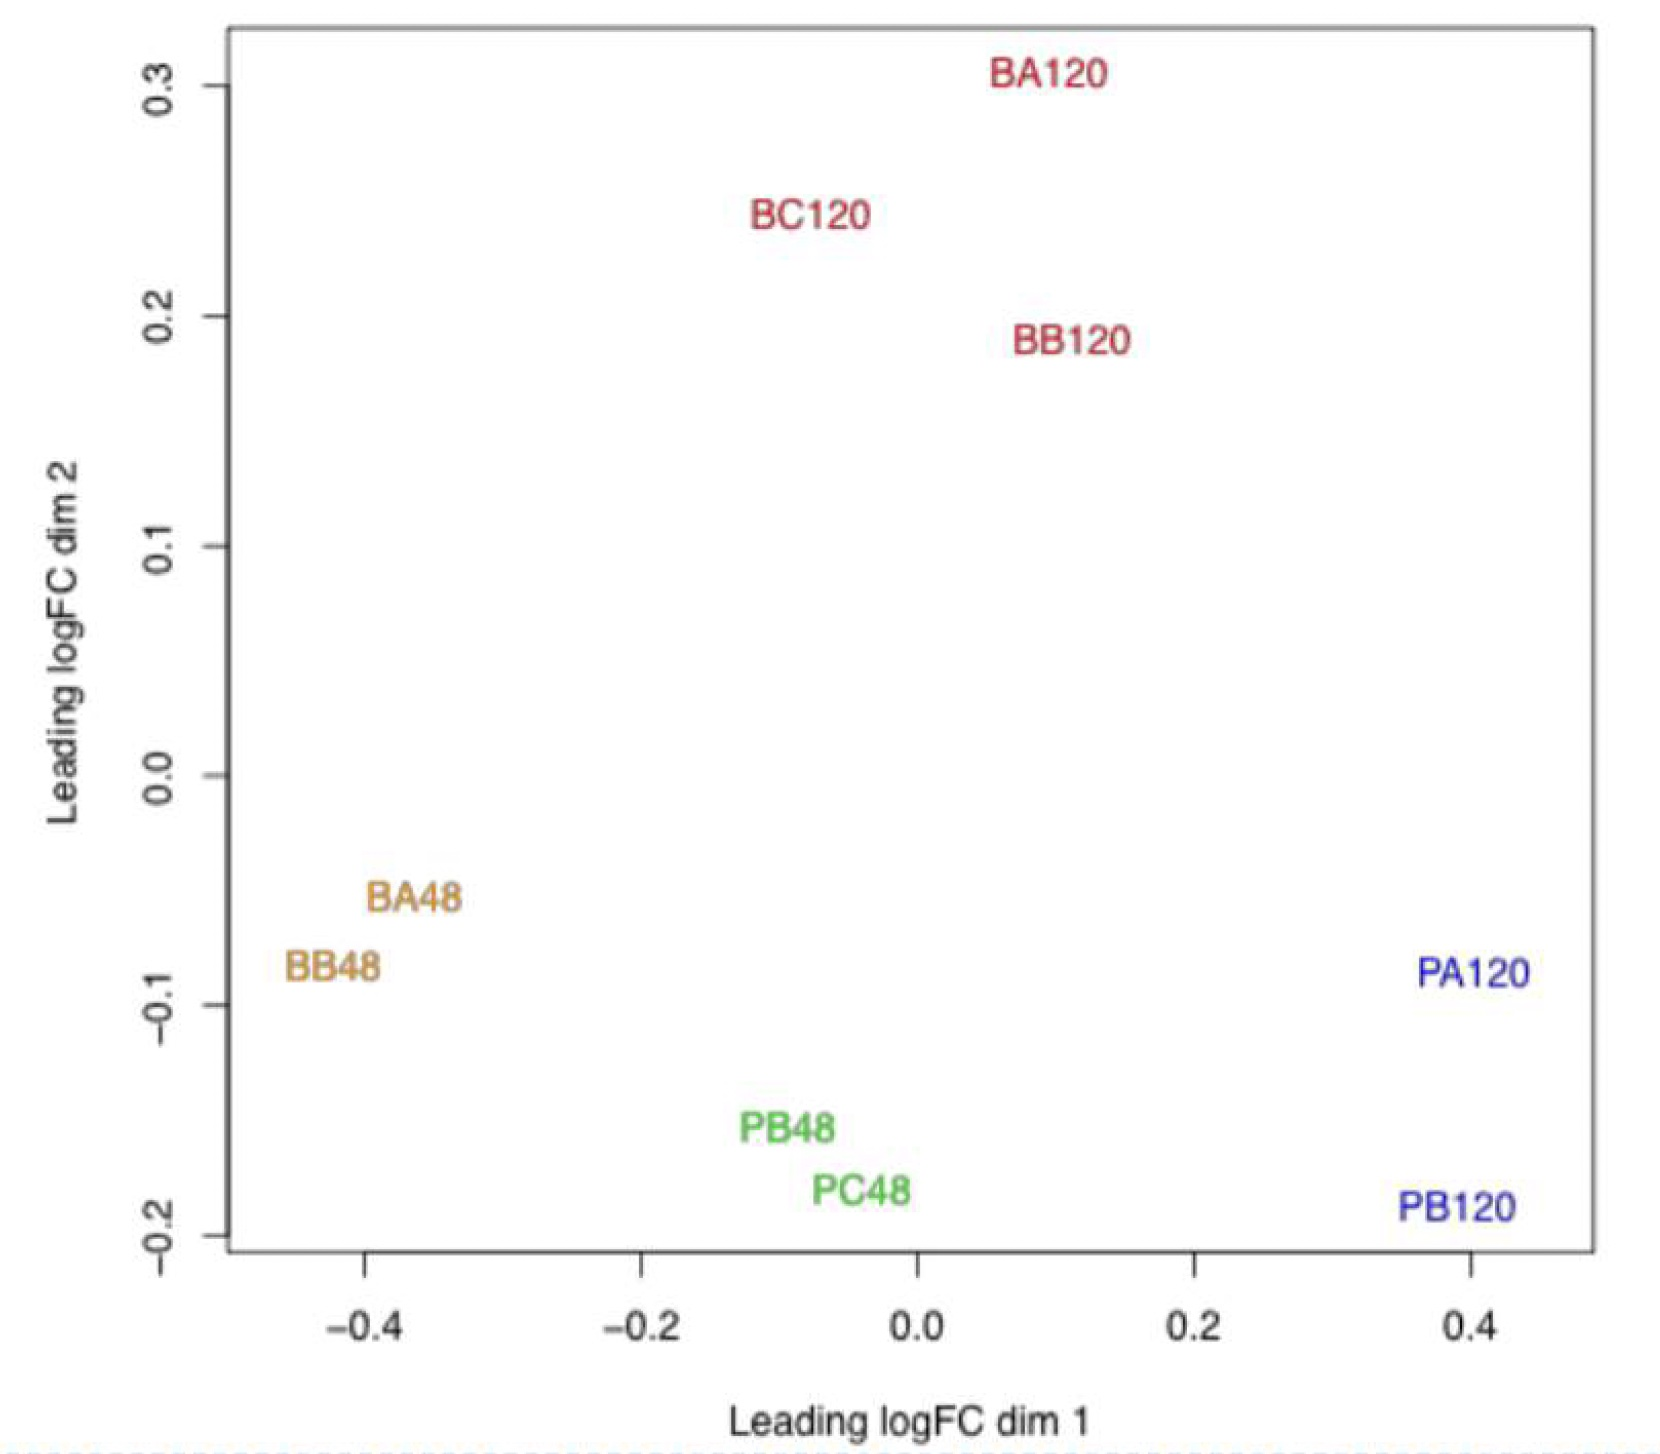
\includegraphics[width=0.7\linewidth]{figuras/mdslepto2016} 

}

\caption{Escalado multidimensional en un experimento de transcriptómica de \textbf{\emph{Leptospira biflexa}}. El experimento incluía dos factores, la fase de crecimiento (biofilm y planctónica) y dos tiempos (48 y 120 horas), en 3 réplicas (A, B y C) por condición. Alguna de las réplicas fue descartada por motivos de calidad (figura tomada de Iraola et al. (\citeproc{ref-Iraolaetal2016}{2016})).}\label{fig:mdslepto}
\end{figure}

Con las tecnologías de segunda generación (Roche 454, Illumina, SOLiD) era y aún es común secuenciar fragmentos, como vimos recién. Sin embargo, con tecnologías de tercera generación como la de \textbf{Oxford Nanopore Technologies} es común secuenciar toda la molécula de \textbf{16S} ya que el largo de la lectura no está determinado \emph{a priori} (como sí en Illumina) y es normal obtener \textbf{reads} (lecturas del secuenciador) de miles o aún decenas de miles de pares de bases. Por otro lado, existen otras formas de metagenómica que no pasan por la secuenciación de una región o de una secuencia en particular. En \textbf{metagenómica funcional} la idea es secuenciar todo el \textbf{ADN} presente en la muestra, en lugar de determinadas secuencias en particular. Esto permite capturar no solo la variabilidad de organismos presentes en la muestra sino que también identificar secuencias de ellos que puedan ser relevantes al problema biológico en cuestión.

Por ejemplo, si un determinado microorganismo se encuentra asociado a un determinado estado patológico de un sistema, conocer las secuencias de genes del mismo puede ser relevante para interpretar los mecanismos de acción del mismo. Asumiendo que el organismo no se encuentre completamente secuenciado y disponible en las bases de datos públicos, la función de las secuencias relevantes se puede deducir a partir del mapeo contra las bases de datos de secuencias anotadas (por ejemplo \textbf{GenBank}), usando \textbf{BLAST}. Por otro lado, si varios organismos están expresando las mismas vías, por ejemplo a causa del exceso de un determinado producto o metabolito en el medio, entonces aparecerá una plétora de secuencias relacionadas por la función, pero provenientes de diferentes organismos.

Un paso más adelante se encuentra la \textbf{metatranscriptómica} que tiene por objetivo la caracterización de todo el \textbf{ARN} mensajero (\textbf{ARNm}) presente en cada muestra. La diferencia más importante con la genómica funcional es que mientras que en esta última cada genoma aporta lo mismo y por lo tanto el factor de ponderación es la proporción de cada taxa (v.g. especie) en la muestra, en la metatranscriptómica existe la misma ponderación, pero también la ponderación por expresión de las secuencias (en realidad un balance entre la tasa de transcripción y la de decaimiento). De esta forma, más allá de identificar qué secuencias están presentes en la muestra, podemos cuantificar (en forma relativa) la ``importancia'' de cada una. Por ejemplo, en situaciones de organismos patógenos, si el mismo está expresando genes de resistencia a antibióticos, podemos identificar las secuencias responsables de esto a través de la \textbf{metatranscriptómica}.

Las aplicaciones de todas estas técnicas, \textbf{metagenómica}, \textbf{metagenómica funcional} y \textbf{metatranscriptómica} han permitido avanzar en varios campos donde entender el funcionamiento del ecosistema microbiológicos es fundamental. Por ejemplo, en agricultura resulta muy claro que desde el punto de vista de las plantas el suelo no es solamente el sustrato y las sustancias químicas disponibles para las mismas; se trata de un ecosistema complejo donde los microorganismos juegan un rol fundamental, tanto los de vida libre como los asociados a las plantas. En este sentido, resulta fundamental entender la diversidad de microorganismos en los distintos suelos, su evolución a lo largo del tiempo y cómo eso se relaciona con la productividad del suelo.

Ejemplos en el área de producción animal también son ubicuos. El rumen es un órgano complejo cuya principal misión consiste en la fermentación de los alimentos ingeridos y la preparación para la posterior absorción de nutrientes a nivel intestinal. Se trata de un ambiente esencialmente anaerobio (ausencia de oxígeno) donde proliferan múltiples microorganismos, entre los que se destacan bacterias, protozoos, arqueas metanogénicas, hongos y virus. La mayor parte de los microorganismos presentes nunca han sido cultivados, en parte por la dificultad de cultivar anaerobios, pero las técnicas de metagenómica han permitido enormes avances al respecto. Claramente, la microbiota ruminal es dinámica y suele verse afectada por diversos factores, que incluyen la dieta, cambios en la fisiología del animal producto de la preñez, cambios ambientales o la estación del año. Los distintos tipos de bacterias que actuan en el rumen (de acuerdo a su función en la digestión) comprenden las celulolíticas, lactolíticas, sacarolíticas, lipolíticas, amilolíticas y metanogénicas ureolíticas, entre otras. Entender cómo las distintas variables afectan la composición de la microbiota ruminal es esencial para predecir los impactos en la salud animal y en la producción.

En salud animal como en salud vegetal resulta fundamental entender cuáles son los patógenos causantes de una enfermedad. En general, muchos de los microoorganismos que se encuentran en el órgano afectado son desconocidos y en muchos casos no son cultivables. Como las condiciones de cultivo suelen ser fundamentales en la bacteriología clásica, existe un sesgo importante en asignar las causas de la patogenicidad a organismos cultivables. Esto nos deja con una parte de la historia conocida y otra parte (posiblemente igual de relevante) sin conocer, ya que en muchos casos el origen de una patología puede ser el producto de un desarreglo en la comunidad que lleve a patógenos oportunistas a tomar la oportunidad. Más aún, uno de los temas de mayor preocupación para la salud mundial, en el paradigma de \textbf{Una Sola Salud} (\textbf{\emph{One Health}}, en inglés) es la resistencia a antibióticos que se ha desarrollado a escala global y que amenaza dejarnos sin tratamiento ante enfermedades que parecían superadas. Frente a esto parece fundamental empezar a trabajar el tema desde una perspectiva racional, tanto a nivel de las políticas y la investigación como a nivel del trabajo de campo. Para un manejo racional es fundamental, a su vez, conocer los organismos causantes de cada patología específica, así como los potenciales mecanismos de resistencia desarrollados, ya que el uso infructuoso de antibióticos no hace otra cosa que aumentar las posibilidades de desarrollar otras resistencias.

En este último sentido, la metagenómica puede constituirse en una herramienta muy poderosa para la invetigación, por ejemplo en el estudio de la mastitis bovina, analizando los cambios en la flora microbiana de la glándula mamaria en animales sanos cuando pasan a un estado de mastitis. En principio, no solo es posible estudiar la composición microbiana durante la evolución de la enfermedad sino que mediante \textbf{metagenómica funcional}, y especialmente mediante \textbf{metatranscriptómica}, se puede analizar el \textbf{resistoma} (el conjunto de los genes relacionados a la resistencia) de la ubre (Hoque et al. (\citeproc{ref-Hoqueetal2020}{2020})). Además, otras técnicas masivas que ya se están utilizando en forma rutinaria en el diagnóstico de enfermedades infecciosas en humano, como la espectrometría de masas MALDI-TOF\footnote{Técnica analítica que permite determinar con alta precisión qué moléculas orgánicas y/o biomoléculas se encuentran presentes en una muestra.}, prometen revolucionar la velocidad y precisión de diagnóstico en animales de producción, así como mejorar la predicción de resistencias antes de aplicar antibióticos (Nonnemann et al. (\citeproc{ref-Nonnemannetal2019}{2019})).

\subsection*{Ejemplo 1.2}\label{ejemplo-1.2}
\addcontentsline{toc}{subsection}{Ejemplo 1.2}

Interpretar la Figura \ref{fig:mdslepto} sabiendo que la letra inicial (``P'' de planctónica, es decir vida libre, o ``B'' de biofilm) representa la fase del crecimiento de colonias de la bacteria \textbf{\emph{Leptopsira interrogans}}, la segunda letra representa la réplica biológica del experimento (``A'', ``B'' o ``C'', para tres réplicas) y los número finales representan las horas a las que se extrajo la muestra a partir del inicio del experimento.

En general, en todos los experimentos biológicos donde queremos generalizar las conclusiones a la población debemos incluir una muestra representativa de individuos a comparar. Los experimentos de transcriptómica son lo suficientemente complejos y caros como para que el número de réplicas no sea elevado (3 por condición, en este caso).

Originalmente se trata de un experimento factorial balanceado del tipos 2x2, ya que tenemos dos factores (la fase de crecimiento -vida libre o biofilm- y los tiempos -48 y 120 horas-), cada uno con dos niveles; en cada celda del diseño factorial tenemos 3 réplicas. Se trata de un experimento de RNA-seq (transcriptómica), por lo que los datos que originan el gráfico salen de una tabla de conteo de ``\emph{reads}''.

Lo primero que se observar en la figura es que algunas muestras fueron descartadas del análisis, de acuerdo con los autores debido a que no cumplían los requisitos de calidad previamente establecidos. Lo segundo que se observa es que las muestras se agrupan razonablemente de acuerdo a la condición biológica, es decir, cada celda del diseño factorial (que están representadas por distintos colores). Seguramente, las muestras no consideradas caerían lejos de su grupo correspondiente (lo que no es criterio para descartarlas), pero también lejos de de todas las otras muestras.

Finalmente, la distribución de las muestras no sigue el patrón de que cada celda del diseño factorial (cada color en el gráfico), ocupe un cuadrante diferente, en particular cada eje representando uno de los factores. Entonces, podemos deducir que la relación entre los factores y las fuentes de varianción no es totalmente ortogonal (\emph{i.e.}, no son totalmente independientes). Sin embargo, es posible trazar una línea que divida a las de vida libre (planctónicas) de las sésiles (biofilm) y otra línea que separe las de 48 hs vs las de 120 horas (de hecho, infinitas de estas rectas en ambos casos), por lo que parece existir ``buena biología'' en las causas de la separación.

\begin{graybox}

\begin{itemize}
\tightlist
\item
  Para entender la variabilidad genética es necesario conocer las secuencias, o al menos algunas secuencias que nos puedan servir de marcador, en muchos individuos. Los \textbf{\emph{microarrays}} son un arreglo de \textbf{sondas moleculares} colocadas en una placa.
\item
  Una \textbf{sonda molecular}, en este caso, es una \textbf{secuencia específica a un gen o una región de un gen y que es (idealmente) única en el genoma de referencia}. Cuando el ADN o el ADN copia (en los estudios de transcriptómica) de un individuo se hibrida con dicha sonda (que está fijada en la placa) se produce algún tipo de señal, por ejemplo la emisión de luz en determinada frecuencia al ser iluminada por un laser. Esta tecnología permite, por ejemplo, identificar si la secuencia presente en el organismo es de un tipo u otro en el caso de los \textbf{SNPs} (polimor- fismos de un solo nucleótido) e identificar el genotipo en el caso de las especies diploides.
\item
  Es importante tener en cuenta que para crear una sonda para medir variabilidad hay que conocer de antemano las secuencias de regiones que contengan variabilidad, y que el \emph{array} solo va a captar variabilidad en las posiciones del genoma para el que fue diseñado.
\item
  La \textbf{metatranscriptómica} tiene por objetivo la \textbf{caracterización de todo el ARN mensajero (ARNm)} presente en cada muestra. La diferencia más importante con la genómica funcional es que mientras que en esta última cada genoma aporta lo mismo y por lo tanto el factor de ponderación es la proporción de cada taxa (\emph{v.g.}, especie) en la muestra, en la metatranscriptómica existe la misma ponderación, pero también la ponderación por expresión de las secuencias. De esta forma, más allá de identificar qué secuencias están presentes en la muestra, podemos cuantificar (en forma relativa) la ``importancia'' de cada una.
\end{itemize}

\end{graybox}

\section{Genómica composicional}\label{genuxf3mica-composicional}

Si bien todos los organismos derivan del mismo organismo ancestral (\textbf{LUCA}) y por lo tanto deben compartir ciertas características en sus genomas, los mismos evolucionan y son la base de las diferencias entre los distintos organismos. A nivel genómico la evolución se da por un conjunto de eventos como las mutaciones puntuales, las duplicaciones de genes y regiones, o las inserciones y ``deleciones'' de secuencias nucleotídicas. Claramente, la mayor parte de estos eventos producen cambios importantes a nivel composicional de los genomas. Por ejemplo, las mutaciones pueden llevar a una acumulación de cambios completamente al azar en los genomas, o puede tener determinados tipos de sesgos que favorezcan que las mutaciones sean hacia determinadas bases (por ejemplo, mutaciones desde las bases A y T hacia las base G y C; recordar que en el ADN doble cadena A se aparea con T y C con G). Los eventos de duplicación génica, por otro lado, generan cierta libertad para que ambas evolucionen más libremente, ya que en principio una de las dos secuencias sigue siendo funcional (hasta que también deje de serlo) y de esta forma se pueden explorar nuevas funciones para una de las dos secuencias.

En general, el conjunto de estos cambios hace que resulte interesante para entender las bases de la evolución en ambientes particulares, o aún en general, el conocimiento de las secuencias de los diferentes organismos y la comparación de las mismas. El estudio de las variaciones en la composición de los genomas es lo que se puede llamar \textbf{\emph{genómica composicional}} y forma parte de la \textbf{\emph{genómica comparativa}}. A continuación veremos el tema de la variación en composición, tanto desde el punto de vista de los nucleótidos, como de los codones en las secuencias codificantes y finalmente de los aminoácidos que forman las proteínas.

\subsection*{\texorpdfstring{Contenido GC genómico, génico, correlaciones y \(\text{GC}_{\text{skew}}\)}{Contenido GC genómico, génico, correlaciones y \textbackslash text\{GC\}\_\{\textbackslash text\{skew\}\}}}\label{contenido-gc-genuxf3mico-guxe9nico-correlaciones-y-textgc_textskew}
\addcontentsline{toc}{subsection}{Contenido GC genómico, génico, correlaciones y \(\text{GC}_{\text{skew}}\)}

La proporción de bases guanina y citosina (G y C, respectivamente) que
componen una secuencia se conoce como el contenido GC de la misma, o
G+C, o aún GC\% (cuando expresado en porcentaje)\footnote{El contenido GC se calcula usualmente como
  \(GC=(N_C+N_G)/(N_A+N_C+N_G+N_T)\), donde \(N_A\)...\(N_T\) corresponde
  al número de veces que aparece cada base en una secuencia.}. Por las reglas de
apareamiento de bases (A-T y G-C), no tiene importancia en la
determinación de dicho contenido cual hebra del ADN se considera para el
cálculo de esta proporción.

\begin{recuadro}

\textbf{Reglas de Chargaff}

\begin{itemize}
\tightlist
\item
  \textbf{Primera regla de paridad}
  La primera regla sostiene que una molécula de ADN de doble cadena tiene a nivel global las siguientes igualdades en el porcentaje de bases:\%A=\%T y \%G=\%C. La validación rigurosa de la norma constituye la base del apareamiento de Watson-Crick de la doble hélice del ADN.
\item
  \textbf{Segunda regla de paridad}
  La segunda regla es que tanto \%A∼\%T y \%G∼\%C son válidos para cada una de las dos hebras de ADN. Esto describe solamente una caracterísstica global de la composición de bases en una sola hebra de ADN.
\end{itemize}

\end{recuadro}

En principio, uno podría preguntarse cuál es
la importancia de medir esta proporción en particular y no otra de las
tres posibles combinaciones de dos bases distintas\footnote{Hay 6 de estas
  combinaciones, pero como la frecuencia de las dos elegidas más la de las
  otras dos debe sumar 1, basta con calcular la mitad; \emph{v. gr.}, GC=1-AT.}. Es
más, alguna de ellas resultan obviamente relevantes, como la proporción
de purinas vs.~pirimidinas (AG vs.~CT). Entonces, ¿qué es lo que hace
tan relevante al contenido GC de las secuencias?

\begin{recuadro}

\textbf{Transiciones y transversiones}

\begin{itemize}
\tightlist
\item
  Los cambios entre \textbf{PURINAS} (A y G) o entre \textbf{PIRIMIDINAS} (C y T) se llaman \textbf{transiciones}.
\item
  Los cambios de PURINAS a PRIDIMINAS, o al revés, se llaman \textbf{transversiones}.
\item
  Las transiciones son mucho más frecuentes que las transversiones.
\end{itemize}

\end{recuadro}

Existen varias razones, como veremos más adelante, pero desde el punto de vista bioquímico tal
vez la más obvia sea la diferencia en el número de puentes de hidrógeno
entre los apareamientos A-T y los G-C, dos para el primero y tres para
el segundo, así como diferencias en el ``\emph{stacking}'' resultante\footnote{Los orbitales de los anillos aromáticos de las bases nitrogendas de los nucleótidos que componen la molécula de ADN interaccionan a medida que se apilan en el polímero. Esta interacción no covalente es un factor fundamental que aumenta la estabilidad de la doble hélice de ADN.}. Esto
conduce directamente a importantes diferencias en las propiedades
físicas de la doble hebra. Por ejemplo, existe un incremento en el ``\emph{melting
point}'' (temperatura en la cual la mitad de las dobles hélices de ADN se desnaturalizan) en función del contenido GC
(\citeproc{ref-Yakovchuk_Protozanova_Frank-Kamenetskii_2006}{Yakovchuk, Protozanova, and Frank-Kamenetskii 2006}). Pero más importante
aún, en secuencias codificantes el código genético (tanto el ``universal''
como todas sus variantes) establece un mapeo entre la secuencia de ADN y
la proteína que será traducida a partir de la misma. Dada la estructura
``redundante'' del código genético, algunos aminoácidos presentan poca
dependencia del contenido GC, mientras que otros se encuentran
fuertemente asociados a este problema (ya que los codones
correspondientes tienen un sesgo importante).

En la Figura \ref{fig:tabcodgene} se aprecia la tabla correspondiente al \textbf{código genético universal}\footnote{Si bien el código genético se encuentra ampliamente conservado en los tres dominios de la vida, este claramente no es universal. Mitocondrias, cloroplastos y algunos protozoarios unicelulares o bacterias del género \emph{Mycoplasma}, entre otros, emplean códigos genéticos con variaciones en algunos codones.}.

\begin{figure}[H]

{\centering 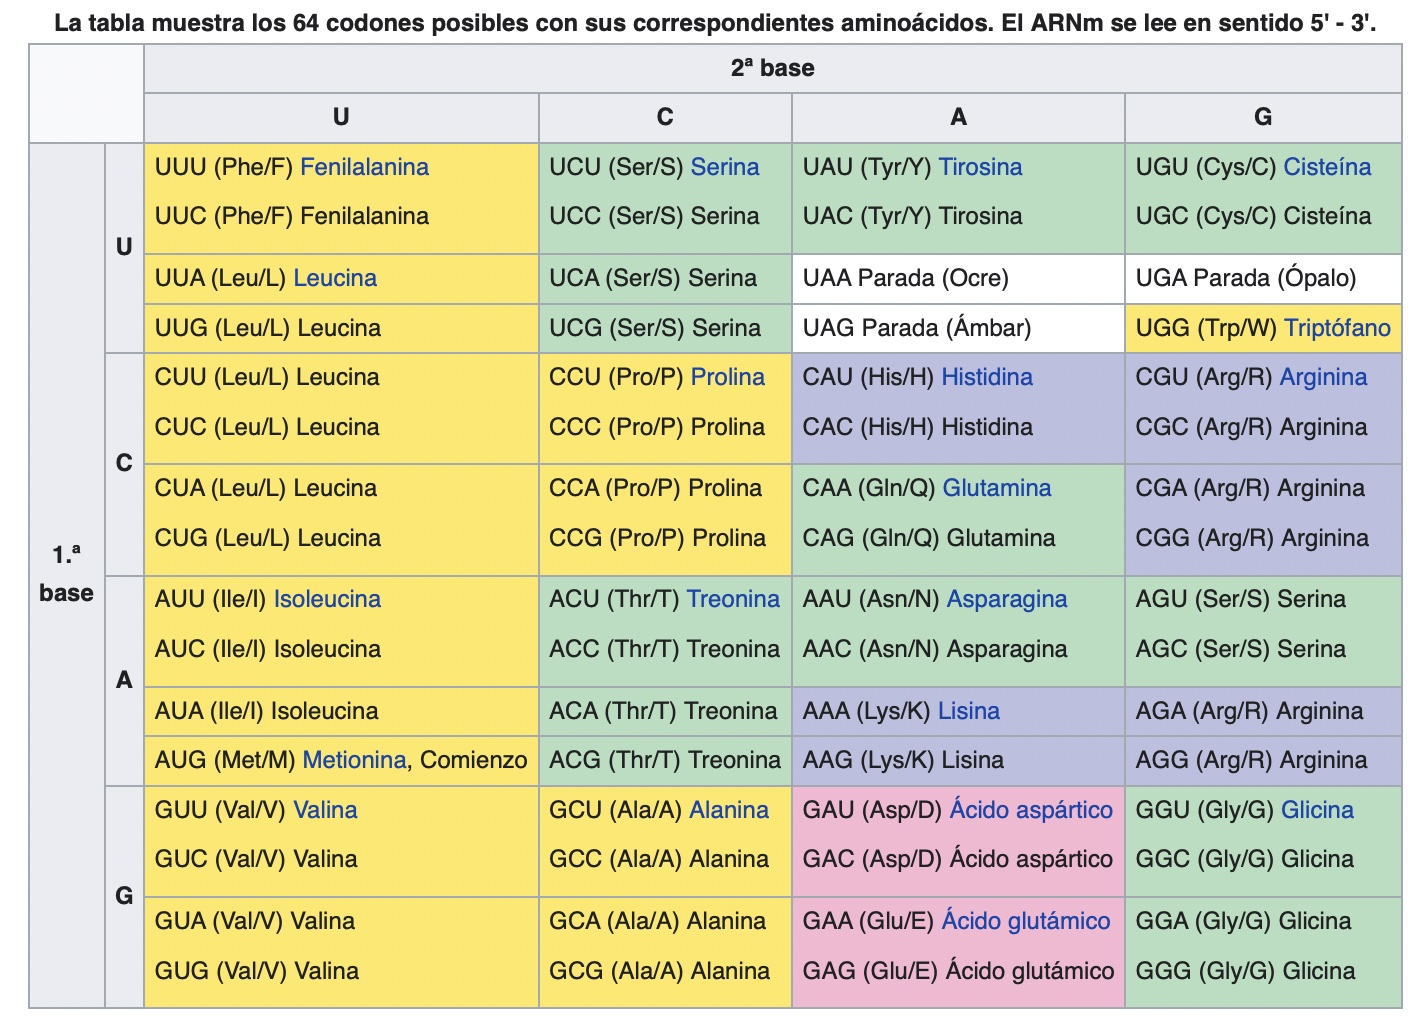
\includegraphics[width=0.7\linewidth]{figuras/tablacodigogeneticoWiki} 

}

\caption{Tabla del código genético universal. En amarillo los aminoácidos apolares, en verdes los polares, azul básicos y rosa ácidos, con blanco correspondiendo a los codones de parada (de Wikipedia, \url{https://es.wikipedia.org/wiki/C\%C3\%B3digo_gen\%C3\%A9tico}).}\label{fig:tabcodgene}
\end{figure}

Claramente, de acuerdo a los colores, que representan propiedades de los aminoácidos, los mismos se encuentran distribuidos en forma bastante organizada de acuerdo a estas propiedades. Cada columna marca una base diferente en segunda posición del codón (U, C, A, G). Por ejemplo, la tercera columna incluye los codones con segunda base \textbf{A} (adenina) y la misma codifica para aminoácidos mayormente codificados por duetos (\emph{i.e.},por dos codones). La primera columna corresponde a codones con segunda base \textbf{U} (uracilo, correspondiente en ADN a \textbf{T}) y codifica para aminoácidos apolares.

\begin{recuadro}

\textbf{Alguna propiedades del código genético universal}

\begin{itemize}
\tightlist
\item
  2 Singletons (Met y Trp), 9 Duetos (Phe, Tyr, His, Gln, Asn, Lys, Asp,
  Glu, Cys), 1 Terceto (Ile), 5 Cuartetos (Val, Pro, Thr, Ala, Gly) y
  3 Sextetos (Leu, Ser, Arg).
\item
  La tercera columna (A en la segunda base) codifica duetos: 2/3 de los cambios en tercera base no son sinónimos.
\item
  La primera base del codón es muy conservada: un cambio de bloque-fila implica en general cambio de aminoácido, excepto en sextetos Arg y Leu.
\item
  La segunda base del codón es la más conservada: un cambio de columna implica un cambio de aminoácido.
\item
  La tercera base es la más neutra y por lo tanto menos conservada (rol de los cuartetos).
  Los cambios de aminoácidos (de cuál a cuál) no son todos equivalentes en su impacto: hay cambios conservativos y otros disruptivos.
\end{itemize}

\end{recuadro}

Entre los aminoácidos codificados por codones con un fuerte sesgo GC(AT) tenemos: \textbf{\emph{Phe}} (5 A/T en 6
posiciones), \textbf{\emph{Ile}} (8 A/T en 9) y \textbf{\emph{Tyr}} (5 A/T en 6). ¿Son utilizados estos aminoácidos de forma homogénea en los diferentes genes codificantes de los organismos?. Veamos por
ejemplo cómo es el uso de estos aminoácidos en el genoma de \emph{Buchnera aphidicola str. Cc (Cinara cedri)},
una bacteria parásita intracelular obligada con contenido GC de 20.1\%.
Mientras que en la proteína codificada por la secuencia con mayor contenido GC del genoma (36.7\%) el
uso de estos 3 aminoácidos corresponde al 16\%, en la proteína con menor
contenido GC (8.6\%) el uso de los mismos sube a 48\%. Además, nos podemos preguntar, ¿las diferencias en contenido GC a nivel genómico pueden dar lugar a diferencias en el contenido GC de las secuencias codificantes?. ¿Esto puede llevar a diferencias entre organismos con genomas con contenido GC diferente?. En principio, podemos pensar que estas diferencias
no tendrían de por sí una consecuencia necesaria a nivel de diferencias
entre organismos, ya que de hecho el contenido GC podría ser una simple consecuencia de los aminoácidos constituyentes de las proteínas codificadas en el organismo y no al
revés. Es decir, la distribución del contenido GC de las proteínas de un
organismo podría ser solo el reflejo de la constitución de las mismas.



Sin embargo, de ser esto cierto esperaríamos que organismos con una
composición relativamente similar a nivel de sus proteínas
constituyentes tuvieran similar contenido GC, y esto no es lo que ocurre.
De hecho, es bien conocido que entre los organismos procariotas
(Bacteria y Archaea) el contenido GC genómico varía desde 25\% a 75\%
aproximadamente (\citeproc{ref-Sueoka_1962}{Sueoka 1962}), con algunos organismos aún más extremos. Estas variaciones marcadas se dan incluso entre organismos de un mismo filo. Más aún, la
bacteria \emph{Anaeromyxobacter dehalogenans 2CP-C}, primer cultivo puro de
una \emph{myxobacteria} capaz de crecer en forma anaeróbica, con un contenido
GC genómico de 74.9\%, está constituída por proteínas cuyo contenido GC
va entre 56.5\% y 88.0\%. Comparando esto con los datos de \emph{B. aphidicola}
mencionados anteriormente, observamos que no existe superposición. Es decir, ambas bacterias no
tendrían ninguna proteína de similar composición. Sabemos, sin embargo,
que ambas comparten un origen evolutivo único, y por lo tanto descienden
de un mismo organismo. Además, ambas cuentan con una serie de proteínas
con idéntica función, pero de hecho con la composición aminoacídica de estas es muy
diferente. Claramente, estos hechos van en contra de la línea de razonamiento planteada anteriormente.\\

¿Qué es entonces lo que nos permite pensar que sería el contenido GC el
que conduce el proceso de sustitución de aminoácidos? Hay varios motivos
para pensar en este sentido. El primero es que los procariotas, cuyo
genoma es en su mayoría \textbf{codificante}, poseen una importante homogeneidad
composicional (restringida por la necesidad de usar todos los
aminoácidos). Esto se manifiesta aún en las regiones intergénicas, que
no tienen mayores restricciones composicionales. Un ejemplo del alto
nivel de homogeneidad se puede ver al comparar los intervalos
inter-cuartílicos de contenido GC codificante, que tanto en \emph{B.
aphidicola} como en \emph{A. dehalogenans} es de 6\%; en otras palabras, la
mitad de las proteínas dentro de cada bacteria difieren en menos de 6\%
de contenido GC (comparar contra más de 50\% de diferencia entre el contenido GC del genoma de ellas).

Pero, además, existe otra evidencia fuerte. Así como calculamos el contenido GC de una
secuencia, también podemos calcular el contenido GC en cada una de las
posiciones de los codones de la misma. Como hay tres posiciones por
codón tenemos entonces \(GC_1\), \(GC_2\) y \(GC_3\), de acuerdo al contenido
GC solo considerando una posición a la vez. Si observamos el código
genético con detenimiento vamos a observar que la tercera posición es la
``más sinónima'', es decir, la posición en la que una mayor proporción de
los cambios de base no afectan el aminoácido codificado. De hecho,
excepto \textbf{\emph{Met}} y \textbf{\emph{Trp}}, todos los aminoácidos poseen codones
sinónimos, con opción entre G/C y A/T. De acuerdo con esto, si el
contenido GC no estuviera conduciendo el proceso de sustitución de
aminoácidos, se podría esperar que el \(GC_3\) se mantuviera variando
libremente entre los distintos genomas, con casi tanta varianza entre
como dentro de genomas. Sin embargo esto no es así, ya que existe una
fuerte correlación positiva entre el contenido GC y el \(GC_3\), tanto a
nivel de secuencias como considerando los genomas enteros (en
procariotas) y aún con las regiones intergénicas flanqueantes
(\citeproc{ref-Zerial_Salinas_Filipski_Bernardi_1986}{Zerial et al. 1986}).\\

Además de los sesgos en contenido GC que discutimos más arriba, existen
otros sesgos menos obvios pero con muy importantes consecuencias
prácticas. Por ejemplo, si consideramos una región particular de la
mayoría de los genomas bacterianos es posible observar una diferencia
importante (dentro de cada hebra) entre el número de bases G y C, así
como entre A y T. De hecho, este fenómeno se encuentra asociado a la
replicación de los genomas bacterianos (usualmente circulares) y
típicamente la hebra ``\emph{leading}'' (``líder'', en inglés) se encuentra enriquecida en G y T,
mientras que la ``\emph{lagging}'' (``rezagada'', en inglés) se encuentra enriquecida en C y A. Las
desviaciones de las frecuencias G=C y A=T se conocen como \(\text{GC}*{\text{skew}}\) y
\(\text{AT}*{\text{skew}}\), respectivamente \footnote{El \(GC_{skew}\) se calcula tomando una ventana de tamaño
  determinado y de acuerdo con la siguiente expresión:
  \(GC_{skew}=(N_G-N_C)/(N_G+N_C)\).}. Una aplicación práctica evidente de
esto es la determinación (aproximada) del origen de replicación, ya que
en este (y en la posición opuesta dentro del genoma circular) habrá un
cambio de signo del \(\text{GC}*{\text{skew}}\) (asociado a la densidad de genes en una
hebra y otra). Una forma de visualizar esto es graficando el \(\text{GC}*{\text{skew}}\)
en las ordenadas contra la posición del genoma (centro de la ventana) a
partir del cual fue calculado, identificando el cambio de signo en las
ordenadas. Otra alternativa, generalmente más efectiva, es plotear el
\(\text{GC}_{\text{skew}}\) acumulado contra la posición y observar los máximos y mínimos
del gráfico, que usualmente están a una distancia de medio genoma
(\citeproc{ref-Grigoriev_1998}{Grigoriev 1998}).

Si bien existe una fuerte controversia sobre la explicación causal de
todas estas correlaciones, así como de correlaciones entre el contenido
GC y factores del ambiente donde viven los organismos, resulta claro que el contenido GC
tiene un importante rol en la evolución de los organismos y en los
procesos moleculares que rigen a los mismos (incluso se debe tener en
cuenta a la hora de calcular algunos índices genómicos o en los procesos
bioquímicos que requieran la denaturalización del ADN). Existen diversas
herramientas para el cálculo del contenido GC, alguna de ellas web
(\emph{\href{http://v.gr/}{v.gr}.}, Mobyle \url{http://mobyle.pasteur.fr/}) que sirven para un cálculo
rápido de una o pocas secuencias. Sin embargo, si el cálculo involucra
muchas secuencias lo usual es recurrir a la programación de tipo
``\emph{scripting}'', usualmente en lenguajes como \emph{Python}
(\url{http://python.org/}), \emph{Perl} (\url{http://www.perl.org/}), o \emph{Java}
(\href{http://www.java.com/}{http://www.java.com}; todos ellos poseen módulos ``Bio'' que facilitan
todas las tareas), en \emph{R} (\url{http://cran.r-project.org/}) a través de
bibliotecas como \emph{seqinr}, en bash (cuando se trabaja en Linux-UNIX o
Mac OS-X), o usando paquetes como \emph{EMBOSS}
(\url{http://emboss.sourceforge.net/}). Si se desea trabajar con genomas
procariotas ya secuenciados, una página interesante es la de OligoWeb
(\url{http://insilico.ehu.es/oligoweb/}), ya que además de las frecuencias de
nucleótidos de los distintos genomas ya tiene calculados otros índices y
estadísticos.\\

\subsection*{Uso de codones}\label{uso-de-codones}
\addcontentsline{toc}{subsection}{Uso de codones}

Habíamos hablado antes de que los genomas procariotas eran
extremadamente amplios en el rango de contenidos G+C y que, dado lo
reducido de lo no-codificante, estas variaciones debían tener
implicancias en el uso de codones. Es más, si comparamos entre genomas
veremos que existe una clara correlación lineal entre el contenido GC
del genoma con \(GC_1\), \(GC_2\) y \(GC_3\), aunque con diferentes
pendientes. En general \(GC_3\) es una posición sinónima, es decir al cambiar
de base en ella no hay cambio de aminoácido (debido a la degeneración
del código genético; ver los cuartetos por ejemplo). \(GC_1\) y \(GC_2\) son mucho
más restringidas en su variación, dado que suelen implicar un cambio de
aminoácido, lo que por lo general afecta negativamente la función de la proteína donde sucede dicho cambio.

Esta redundancia en el código genético, sumado a las posibilidades de
reconocimiento alternativo codón/anticodón (no-Watson-Crick), permiten la
evolución en los genomas de diferentes estrategias de uso de codones
(UC) (\citeproc{ref-Rocha_2004}{Eduardo P. C. Rocha 2004}). Esto, que puede verse entre genomas, también tiene su
correlato a nivel interno en muchos genomas. Es conocido que en algunos
genomas procariotas los genes altamente expresados tienden a usar
\textbf{codones mayores}, que suelen ser reconocidos en forma de apareamiento Watson-Crick por los tRNAs más abundantes, aunque hay distintos modelos (ver la discusión en
(\citeproc{ref-Rocha_2004}{Eduardo P. C. Rocha 2004})). Lograr comprender los factores que inciden en el uso de
codones (también puede pensarse para aminoácidos) suele requerir de
alguna forma de ``resumir'' la información.\\

En un genoma procariota promedio tenemos unos 4000 genes y los codones
de aminoácidos con degeneración son 59 (los 64 menos los 3 \emph{stop}, menos
\textbf{\emph{Met}} y \textbf{\emph{Trp}}, que son codificados por un único codón cada uno), lo que se puede resumir en una tabla de esas
dimensiones. Utilizando la misma, podríamos analizar si distintos genes utilizan de forma diferente los codones, e hipotetizar cuál puede ser el motivo subyacente a este fenómeno. Para quitar la influencia
del uso de aminoácidos como factor que influye en esta perspectiva (cada
proteína tiene un uso diferencial de AAs), se puede estandarizar a la
interna de cada aminoácido. Una de las estandarizaciones posibles es el
\emph{RSCU} (\citeproc{ref-Sharp_Tuohy_Mosurski_1986}{Sharp, Tuohy, and Mosurski 1986}), en el que el número observado de
codones para un aminoácido es dividido por el número esperado si el uso
dentro de un aminoácido fuera equiprobable. Es decir,

\begin{equation}
\text{RSCU}*{ij}=\frac{x*{ij}}{\frac{1}{n_i}\sum_{j=1}^{n_i}\ x_{ij}}
\label{eq:rscu1}
\end{equation}

donde \(x_{ij}\) es el número de ocurrencias del codón \(j\) para el
aminoácido \(i\) y \(n_i\) es la multiplicidad del aminoácido \(i\) (es decir, el número de codones que lo codifican).

De cualquier forma, aún luego de estandarizar seguimos teniendo la tabla
de 4000x59 (\emph{i.e.} cada gen en una fila, y el índice RSCU calculado para cada uno de los 59 codones considerados). La mayor parte de los humanos tenemos una limitada capacidad
para visualizar datos en espacios de más de 3 dimensiones, por lo que
necesitamos reducir la ``dimensionalidad'' del problema. Podríamos pensar
en representar las 59 variables originales de a pares
(\(\binom{59}{2}=59*58/2=1711\)), o aún de a tres
(\(\binom{59}{3}=59*58*57/6=32509\)) para ver interacciones entre más
variables, pero estos números hacen imposible poder extraer conclusiones
relevantes en forma sistemática. Afortunadamente, existen diferentes técnicas
estadísticas exploratorias multivariadas que nos permiten abordar este
tipo de cuestiones.

Probablemente, de las técnicas usuales de análisis exploratorio multivariado, la más conocidas es el \textbf{Análisis de Componentes Principales} (PCA, del inglés \emph{Principal Component Analysis}), aunque existen otros miembros prominentes
de la familia. Uno de los más interesantes para nuestro tipo de problema
es el \textbf{Análisis de Correspondencia} (COA, ver Sección \hyperref[exploracion-multivariada]{Exploración multivariada: Análisis de Correspondencia}). El mismo
nos permite reducir la variación en las 59 variables originales a unas
pocas dimensiones (cada una de ellas una combinación de las originales) que capturan la mayor parte de la variabilidad. De esta forma, el
problema pasa a ser identificar qué variables biológicas se asocian a
cada una de estas dimensiones.

Ejemplos típicos de variables biológicas
asociadas a la variación en el \textbf{uso de codones} dentro de genomas procariotas son el
\textbf{contenido GC del gen}, su \textbf{nivel de expresión}, la \textbf{hidropatía} promedio de
la proteína, la \textbf{hebra} en que se encuentra el gen, el \(\text{GC}_{\text{skew}}\) y la
\textbf{precisión en la traducción} (\citeproc{ref-Ermolaeva_2001}{Ermolaeva 2001}). Diferencias en el uso de codones entre
genomas han sido reportadas asociadas a varios factores
eco-fisiológicos, entre ellos la \textbf{temperatura óptima de crecimiento} y
adaptaciones a hiper-salinidad. Un programa diseñado específicamente
para el análisis composicional es el \emph{codonW}
(\url{http://codonw.sourceforge.net/}), que analiza las frecuencias de
bases, codones y aminoácidos, calcula diferentes índices estadísticos,
así como permite realizar un COA en codones y AAs.

Existen diversos índices, calculados a partir de las frecuencias de
codones, que permiten identificar sesgos importantes en UC, que pueden
ser suficientemente indicativos de por sí, o combinados con la
información del COA. Por ejemplo, el \emph{Nc} (número efectivo de codones)
es un índice del uso de codones intragénico. Puede tomar valores
extremos de 20, cuando un solo codón por aminoácido es utilizado en ese gen, a
61, cuando hay una equi-distribución de los mismos (\citeproc{ref-Wright_1990}{F. Wright 1990}). Este
índice es sensible al contenido GC del genoma, y una mejora fue sugerida
posteriormente que toma en cuenta este factor (\citeproc{ref-Novembre_2002}{Novembre 2002}). Otros
dos índices, ``codon bias index'' (\emph{CBI}) y ``frequency of optimal codons''
(\emph{Fop}), calculan el sesgo a partir de un juego de codones ``óptimos'',
derivados respectivamente de un conjunto particular de genes o de la
concentración de los tRNAs. Una aproximación totalmente diferente, que
no depende de un conjunto particular de genes, es el ``Codon Adaptation
Index'' (\emph{CAI})(\citeproc{ref-Sharp_Li_1987}{Sharp and Li 1987}), que ha demostrado ser un indicador muy
razonable del nivel de expresión de los genes (basado en comparaciones
con técnicas para medir experimentalmente la expresión génica, como los
\emph{microarrays}). El \emph{CAI} es simplemente la media geométrica de los
\emph{RSCU} relativos (al máximo \emph{RSCU} para ese AA) de todos los codones de
una proteína. Con la misma notación que más arriba, si consideramos
\(\text{w}*{ij}=RSCU*{ij}/RSCU_{i,max}\), entonces se define
\(\text{CAI}=\exp({\frac{1}{L}\sum_{k=1}^L\ln \text{w}_{ij}})\).

Pese a los buenos
resultados del \emph{CAI}, el mismo presenta también importantes debilidades,
como la no-linealidad y una sobre-estimación de las desviaciones para
secuencias cortas. En el 2009, Roymondal y colaboradores
(\citeproc{ref-Roymondal_Das_Sahoo_2009}{Roymondal, Das, and Sahoo 2009}) proponen una aproximación muy diferente,
basada en las frecuencias de cada base en las distintas posiciones de
los codones, que lleva al índice \emph{RCB}. Estos autores proponen para cada
codón \emph{xyz} calcular el \(\text{RCB}\) de acuerdo a la fórmula:

\begin{equation}
\text{RCB}_{xyz}=\frac{f(xyz)}{f_1(x)f_2(y)f_3(z)}
\label{eq:rcb1}
\end{equation}

(donde \(f_1(x)\), \(f_2(y)\), \(f_3(z)\) son las frecuencias de las bases \(x\), \(y\) y
\(z\) en las posiciones 1, 2 y 3 respectivamente), para luego resumir toda
la información a través de la media geométrica,
\(RCB=(\prod_{l=1}^LRCB_{xyz}(l))^{1/L}-1\). Este nuevo índice presenta
ventajas respecto al \emph{CAI}, pero aún presenta un problema importante
para secuencias cortas, lo que llevó a sugerir una modificación del
mismo (\emph{Relative Codon Adaptation}, \emph{RCA}), basada en el uso de
pseudo-conteos (\citeproc{ref-Fox_Erill_2010}{Fox and Erill 2010}).

Un índice de expresión tiene mucha utilidad en la exploración de los
factores que influyen en la composición diferente de los genes, pero un
punto interesante es la posible relación entre la expresión y el
efecto de ``\emph{gene dosage}'' (más copias de genes disponibles a medida que la
replicación avanza), resultado de favorecer los genes altamente
expresados en una posición cercana al origen de replicación. Para
investigar este efecto basta con ver cual es la relación entre el \emph{CAI}
y la posición. Una forma fácil consiste en un análogo del \(GC_{skew}\)
acumulado, calculados como desvíos del \emph{CAI} promedio y compararlo con
las posiciones genómicas. Si existe un efecto de ``\emph{gene dosage}'' el patrón
de \emph{CAI} debería mostrar un pico en la zona del origen de replicación.

Un soporte adicional a la hora de entender lo que ocurre en el uso de
codones cuando comparamos dos grupos, por ejemplo genes de alta
expresión con los de baja expresión, es a través de las tablas de uso de
codones. Las mismas contienen el conteo total por codón para cada grupo
y si las agrupamos por AA podemos calcular la probabilidad de que las
diferencias en uso de codones (para cada codón) se deban al azar. Para
esto, dentro de cada AA se contruye una tabla de 2x2 (2 grupos a
comparar y codón a analizar vs la suma de los otros dentro de AA) y con
la misma realiza un test de \(\chi^2\) con un grado de libertad. Es
importante tener en cuenta las múltiples comparaciones a realizar (el
número de hipótesis a ensayar; \emph{\href{http://v.gr/}{v.gr}.}, el número de codones) a la hora de
definir el umbral de significancia para corregir adecuadamente.

Finalmente, el uso de codones de un organismo puede tener implicancias
directas de carácter tecnológico. Como vimos más arriba, dentro de las
mayores fuentes de variación en UC se encuentra en algunos organismos la
expresión, con codones muy usados en los genes de alta expresión y un
uso más plano en proteínas de baja expresión. Esto influye inclusive en
el plegamiento de las proteínas, cambiando la solubilidad de la misma
(\citeproc{ref-Cortazzo_Cervenansky_Marin_Reiss_Ehrlich_Deana_2002}{Cortazzo et al. 2002}). Cuando deseamos
expresar proteínas recombinantes resulta muy importante considerar no
solo la secuencia de AAs de la proteína a expresar, sino también que el
UC se adapte al UC en genes de alta expresión en el organismo hospedero.

\subsection*{Ejemplo 1.3}\label{ejemplo-1.3}
\addcontentsline{toc}{subsection}{Ejemplo 1.3}

Teniendo en cuenta todas las secuencias codificantes, en una bacteria de interés biotecnológico se observó el siguiente conteo de codones para dos aminoácidos:

\begin{table}
\centering
\begin{tabular}[t]{lll}
\toprule
Aminoácido & Codón & Conteo\\
\midrule
\cellcolor{gray!10}{Arg (R)} & \cellcolor{gray!10}{CGU} & \cellcolor{gray!10}{$666$}\\
Arg (R) & CGC & $1320$\\
\cellcolor{gray!10}{Arg (R)} & \cellcolor{gray!10}{CGA} & \cellcolor{gray!10}{$1457$}\\
Arg (R) & CGG & $1818$\\
\cellcolor{gray!10}{Arg (R)} & \cellcolor{gray!10}{AGA} & \cellcolor{gray!10}{$5913$}\\
\addlinespace
Arg (R) & AGG & $5120$\\
\cellcolor{gray!10}{Val (V)} & \cellcolor{gray!10}{GUU} & \cellcolor{gray!10}{$7123$}\\
Val (V) & GUC & $2144$\\
\cellcolor{gray!10}{Val (V)} & \cellcolor{gray!10}{GUA} & \cellcolor{gray!10}{$1125$}\\
Val (V) & GUG & $8213$\\
\bottomrule
\end{tabular}
\end{table}

Calcular el \textbf{RSCU} para cada codón y determinar cuáles son los usados y si hay diferencias entre los aminoácidos en la forma en que usan los codones.

\hfill\break

De acuerdo a la ecuación \eqref{eq:rscu1}, el RSCU se calcula como

\begin{equation}
RSCU_{ij}=\frac{x_{ij}}{\frac{1}{n_i}\sum_{j=1}^{n_i}\ x_{ij}}
\end{equation}

donde \(x_{ij}\) es el número de ocurrencias del codón \(j\) para el aminoácido \(i\). Tenemos dos aminoácidos diferentes, por lo vamos a calcular el RSCU de cada codón dentro de cada aminoácido. Lo primero es obtener la suma de codones en cada aminoácido, por lo que tenemos que para \textbf{Arginina} es igual a \(666+1320+1457+1818+5913+5120=16294\), mientras que para \textbf{Valina} es de \(7123+2144+1125+8213=18605\). Este es el número total de codones para cada uno de los aminoácidos, o lo que es lo mismo, el número de veces que aparece dicho aminoácido en las secuencias codificantes de nuestra bacteria. Para calcular el RSCU alcanza con dividir el número de ocurrencias de cada codón entre el total de veces que se utiliza el aminoácido y multiplicarlo por el número de codones que tiene el aminoácido (\(n_i=6\) en el caso de Arginina, \(n_i=4\) en el caso de Valina, ver el código genético).

Por lo tanto, utilizando la ecuación \eqref{eq:rscu1}, tenemos que por ejemplo, para el codón \textbf{CGU} de la \textbf{Arginina} su RSCU es igual a

\begin{equation}
RSCU_{R,CGU}=\frac{x_{CGU}}{\frac{1}{6}\sum_{j=1}^6\ x_{R,j}}=6 \times \frac{666}{16294}=0,2452
\end{equation}

Para el codón \textbf{CGC} la cuenta es igual a

\begin{equation}
RSCU_{R,CGC}=\frac{x_{CGC}}{\frac{1}{6}\sum_{j=1}^6\ x_{R,j}}=6 \times \frac{1320}{16294}=0,4861
\end{equation}

y así sucesivamente con todos los codones de este aminoácido, lo que nos deja con una tabla como la siguiente:

\begin{table}
\centering
\begin{tabular}[t]{lll}
\toprule
Codón & Conteo & RSCU\\
\midrule
\cellcolor{gray!10}{$\textbf{CGU}$} & \cellcolor{gray!10}{$666$} & \cellcolor{gray!10}{$0,2452$}\\
$\textbf{CGC}$ & $1320$ & $0,4861$\\
\cellcolor{gray!10}{$\textbf{CGA}$} & \cellcolor{gray!10}{$1457$} & \cellcolor{gray!10}{$0,5365$}\\
$\textbf{CGG}$ & $1818$ & $0,6694$\\
\cellcolor{gray!10}{$\textbf{AGA}$} & \cellcolor{gray!10}{$5913$} & \cellcolor{gray!10}{$2,1774$}\\
\addlinespace
$\textbf{AGG}$ & $5120$ & $1.8854$\\
\cellcolor{gray!10}{$\textbf{Suma}$} & \cellcolor{gray!10}{$16294$} & \cellcolor{gray!10}{$6$}\\
\bottomrule
\end{tabular}
\end{table}

De la misma manera, para la Valina, el RSCU del primer codón es igual a

\begin{equation}
RSCU_{V,GUU}=\frac{x_{GUU}}{\frac{1}{4}\sum_{j=1}^4\ x_{V,j}}=4 \times \frac{7123}{18605}=1,5314
\end{equation}

mientras que para el resto de los codones se calcula en forma análoga, hasta obtener la siguiente tabla:

\begin{table}
\centering
\begin{tabular}[t]{lll}
\toprule
Codón & Conteo & RSCU\\
\midrule
\cellcolor{gray!10}{$\textbf{GUU}$} & \cellcolor{gray!10}{$7123$} & \cellcolor{gray!10}{$1,5314$}\\
$\textbf{GUC}$ & $2144$ & $0,4610$\\
\cellcolor{gray!10}{$\textbf{GUA}$} & \cellcolor{gray!10}{$1125$} & \cellcolor{gray!10}{$0,2419$}\\
$\textbf{GUG}$ & $8213$ & $1,7658$\\
\cellcolor{gray!10}{$\textbf{Suma}$} & \cellcolor{gray!10}{$18605$} & \cellcolor{gray!10}{$4$}\\
\bottomrule
\end{tabular}
\end{table}

En ambos aminoácidos se observa que el uso de codones se aparta bastante de la hipótesis de uso similar. Mientras que en el primer caso (Arginina) los codones favorecidos son los codificados por el dueto (del sexteto), es decir \textbf{AGA} y \textbf{AGG}, en el segundo caso (Valina) los codones favorecidos son los que terminan en \textbf{U} o en \textbf{G}.

\subsection{Exploración multivariada: Análisis de Correspondencia}\label{exploracion-multivariada}

Este método fue desarrollado por Benzecrí (\citeproc{ref-Benzecri_1980}{Benzecri 1980}), originalmente para trabajar con tablas de frecuencias.
En resumen, la idea subyacente es dada una tabla de \(n \times p\) (casos x
variables) encontrar un sistema de \(k\) ejes ortogonales (con
\(k < min(n,p)\)) que condense el máximo de variación en los datos
originales. Esto es posible en la medida en que las variables (casos)
estén correlacionados en alguna medida y cuanto mayor sea esa asociación
más varianza será condensada en pocos ejes (dimensiones). La métrica
adoptada es la de la distancia \(\chi^2\), o sea, para la celda correspondiente a la fila \(i\) y columna \(j\), la distancia será

\begin{equation}
d_{ij}=(O_{ij}-E_{ij})^2/E_{ij}
\label{eq:dchi2}
\end{equation}

donde \(O_{ij}\) es el número observado y \(E_{ij}\) el número esperado para esa celda, usualmente el número total de observaciones multiplicado por las frecuencias relativas marginales en la tabla.

Aplicando el COA a una tabla de frecuencias observadas vamos a obtener una serie de valores
propios y vectores propios asociados (``eigen-values'' y ``eigen-vectors''),
tantos como el mínimo de Filas-1 y Columnas-1. Cada uno de los valores
propios está relacionado con la varianza explicada por la nueva
dimensión correspondiente. La suma de todos los valores propios es
equivalente al 100\% de la varianza por lo que cada uno explicará una
fracción correspondiente al valor propio sobre la suma de todos (la
traza de la matriz de valores propios). A su vez, cada uno explica menor
varianza que el anterior (están ordenados por el procedimiento de
extracción). El punto importante es determinar con cuántos ejes (nuevas
dimensiones) nos vamos a quedar. Cuantas más dimensiones retengamos
mayor cantidad de la varianza original retendremos, pero al costo de
dificultar la interpretación (el objetivo del COA es poder capturar la
esencia de los datos, cuantas más dimensiones más difícil de visualizar
la situación). Existen varios métodos para determinar el número de
dimensiones a retener, pero en última instancia esto es una materia
subjetiva. Un enfoque es gráfico (``\emph{scriplot}'') y consiste en encontrar el
cambio en la pendiente de los valores propios graficados en función de
su número ordinal.

Otra aproximación es retener los valores propios hasta que expliquen menos de lo que se esperaría por azar si cada unas
de las variables originales explicara la misma proporción de la
varianza. Por ejemplo, en una tabla de uso de aminoácidos, dado que hay
20 AAs la varianza promedio explicada por cada uno es 5\% y por lo tanto
luego de un COA en AAs retendríamos todos aquellos valores propios que
expliquen más de 5\% de la varianza. Cada una de las observaciones
originales tendrá ahora unas nuevas coordenadas en el nuevo sistema de
ejes ortogonales (las dimensiones). O sea, si por ejemplo retuvimos de
nuestro COA en uso de AAs 3 dimensiones (combinaciones de las 20
originales) cada gen podrá representarse ahora en un espacio
tridimensional. Asimismo, las variables originales están representadas
de distinta manera en las nuevas dimensiones, es decir tienen distinta
participación en cada una de ellas. Esto apunta a una de las
características más destacables del COA, su simetría Filas/Columnas lo
que permite el auxilio de representar en forma conjunta (en el mismo
gráfico) la distribución de observaciones y variables (genes y AAs, por
ejemplo) aunque las distancias entre observaciones y variables deben
tomarse con cautela.

La clave del éxito con el COA es lograr ``etiquetar'' las nuevas
dimensiones con factores entendibles, biológicamente significativos, que
vayan más allá de las propias variables medidas. Ejemplo de esto en
genómica podría ser la expresión diferencial, los compartimientos
celulares, proteínas IMP (``integral membrane proteins''), etc, cuando se
correlacionan con alguno de los ejes del análisis. La forma tradicional
de trabajo, al menos en el campo de la genómica comparativa, consiste en
determinar cuántos valores propios retener para luego graficarlos de a
pares intentando ver la distribución conjunta de observaciones y
variables en las nuevas dimensiones. Se puede además intentar
correlacionar variables externas con las nuevas dimensiones, buscando
``etiquetas'' para las dimensiones. Un link interesante de análisis de correspondencia:
\url{http://www.micheloud.com/FXM/COR/index.htm}

\subsection{Composición de proteínas}\label{composiciuxf3n-de-proteuxednas}

Hasta ahora hemos centrado nuestros análisis composicionales en bases
nucleotídicas y codones, pero la mayor parte de las secuencias
procarióticas terminan siendo traducidas en proteínas. Por lo tanto, vamos a dedicar un
breve espacio a tratar esta temática. En muchos casos los archivos de partida para un análisis bioinformático (en
cualquiera de los formatos estándar, como FASTA o GenBank) solo incluyen
la secuencia nucleotídica, dado que a partir de la misma es posible
deducir directamente la secuencia de AAs (si conocemos el código
genético correspondiente).

Existen muchos programas para realizar la
traducción de estas secuencias, pero el \emph{transeq} (de la suite \emph{EMBOSS})
es muy flexible y eficiente, aceptando diversos formatos de entrada.
Dentro del \emph{EMBOSS} también tenemos toda una serie de programas para
facilitar el análisis de secuencias proteicas. Entre ellos (hay muchos
más): \emph{antigenic} para encontrar sitios antigénicos, \emph{charge} que hace
un diagrama de carga, \emph{digest} reporta sobre enzimas proteolíticas,
\emph{emowse} para buscar en proteínas por peso molecular de fragmentos de
digestión, \emph{fuzzpro} para buscar patrones, \emph{helixturnhelix} para
identificar motivos de unión a ácidos nucléicos, \emph{iep} para calcular el
punto isoeléctrico, \emph{makeprotseq} para crear secuencias aleatorias,
\emph{pepcoil} para predecir regiones ``coiled-coil'', \emph{pepstats} para calcular
diversos estadísticos de proteínas, \emph{preg} para buscar expresiones
regulares en proteínas, \emph{pepwindow} para realizar un ploteo de
hidropatía, \emph{tmap} para predecir segmentos trans-membrana, \emph{psiphi} para
calcular ángulos torsionales y \emph{patmatmotifs} que escanea una proteína
con motivos del \emph{PROSITE} (\url{http://prosite.expasy.org/}).

\subsection*{Diferencias en propiedades de los AAs}\label{diferencias-en-propiedades-de-los-aas}
\addcontentsline{toc}{subsection}{Diferencias en propiedades de los AAs}

Existen 22 aminoácidos proteinogénicos o naturales (los que se
incorporan directamente en las proteínas). De entre ellos, 20 son
codificados directamente, mientras que la selenocisteína y la
pirrolisina se codifican a partir de modificaciones en la lectura de
codones \emph{stop} (con símbolos IUPAC/IUBMB \textbf{\emph{Sec}} o \textbf{\emph{U}}, y
\textbf{\emph{Pyl}} u \textbf{\emph{O}}, respectivamente). Como se puede apreciar en la
figura \ref{fig:VennAAprop}, los 20 aminoácidos codificados directamente
(que suelen ser los más abundantes) poseen importantes diferencias en
las propiedades físico-químicas, lo que lleva a agruparlos de diferentes
maneras, de acuerdo al grupo de propiedades de relevancia.

Típicamente, podemos distinguir:

\begin{itemize}
\tightlist
\item
  \emph{i)} Polares/hidrofílicos - \textbf{\emph{N}}, \textbf{\emph{Q}},
  \textbf{\emph{S}}, \textbf{\emph{T}}, \textbf{\emph{K}}, \textbf{\emph{R}}, \textbf{\emph{H}}, \textbf{\emph{D}}, \textbf{\emph{E}}, (\textbf{\emph{C}},
  \textbf{\emph{Y}})\footnote{figuran entre paréntesis cuando entran en la categoría parcialmente},
\item
  \emph{ii)} No-polares / hidrofóbicos - (\textbf{\emph{G}}), \textbf{\emph{A}},
  \textbf{\emph{V}}, \textbf{\emph{L}}, \textbf{\emph{I}}, \textbf{\emph{P}}, \textbf{\emph{Y}}, \textbf{\emph{F}}, \textbf{\emph{W}}, \textbf{\emph{M}},
  \textbf{\emph{C}},
\item
  \emph{iii)} enlace de H - \textbf{\emph{C}}, \textbf{\emph{W}}, \textbf{\emph{N}}, \textbf{\emph{Q}},
  \textbf{\emph{S}}, \textbf{\emph{T}}, \textbf{\emph{Y}}, \textbf{\emph{K}}, \textbf{\emph{R}}, \textbf{\emph{H}}, \textbf{\emph{D}}, \textbf{\emph{E}},
\item
  \emph{iv)} contienen azufre - \textbf{\emph{C}}, \textbf{\emph{M}},
\item
  \emph{v)} con carga negativa a
  \emph{pH} neutro / acídicos - \textbf{\emph{D}}, \textbf{\emph{E}}, (\textbf{\emph{C}}),
\item
  \emph{v)} con carga positiva a \emph{pH} neutro / básicos - \textbf{\emph{K}}, \textbf{\emph{R}}, (\textbf{\emph{H}}),
\item
  \emph{vi)} Ionizables - \textbf{\emph{D}}, \textbf{\emph{E}}, \textbf{\emph{H}}, \textbf{\emph{C}}, \textbf{\emph{Y}}, \textbf{\emph{K}},
  \textbf{\emph{R}},
\item
  \emph{vii)} Aromáticos - \textbf{\emph{F}}, \textbf{\emph{W}}, \textbf{\emph{Y}}, (\textbf{\emph{H}}, pero
  sin absorción significativa de UV), \emph{viii )} Alifáticos - \textbf{\emph{G}} ,
  \textbf{\emph{A}}, \textbf{\emph{V}}, \textbf{\emph{L}}, \textbf{\emph{I}}, \textbf{\emph{P}},
\item
  \emph{ix)} Forman enlaces covalentes cruzados (puentes di-sulfuro) - \textbf{\emph{C}},
\item
  \emph{x)} Cíclicos - \textbf{\emph{P}}
\end{itemize}

(ver por ejemplo \url{http://www.mcb.ucdavis.edu/courses/bis102/AAProp.html}).\\



\begin{figure}[H]

{\centering 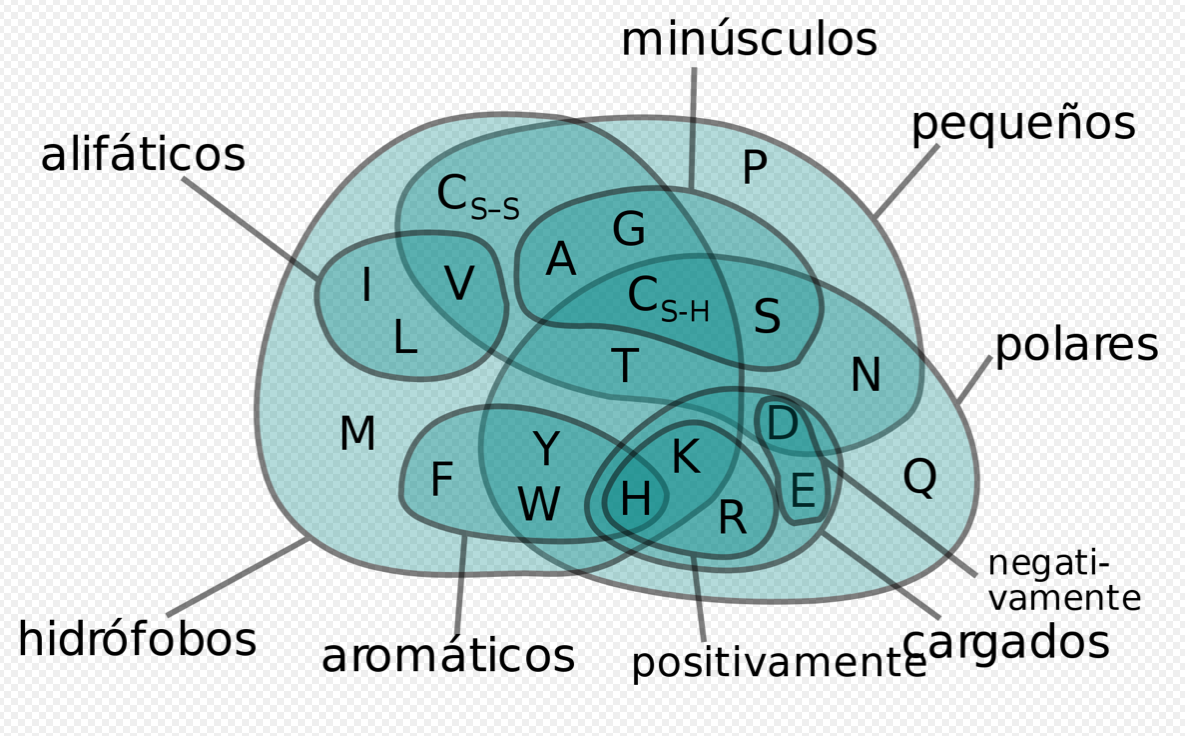
\includegraphics[width=0.7\linewidth]{figuras/VennAApropiedades} 

}

\caption{Diagrama de Venn con las propiedades de los diferentes aminoácidos. Figura tomada de Wikipedia (CC BY-SA 3.0), versión en castellano modificada a partir del archivo ``Amino Acids Venn Diagram (es).svg''}\label{fig:VennAAprop}
\end{figure}

Las diferencias en las propiedades físico-químicas llevan a importantes
diferencias en la estructura de las proteínas y hacen que los cambios
observados (substituciones) entre proteínas homólogas (descendientes de un ancestro común) tengan
distribuciones particulares, las que se suelen representar en matrices
de substituciones\footnote{Las matrices de sustituciones aminoacídicas son matrices que reflejan la frecuencia evolutiva de sustitución de pares de aminoácidos. Existen diferentes variantes (\emph{e.g.} matrices PAM, matriz BLOSUM62), dependiendo del set de proteínas y las asunciones con las que las mismas fueron construídas. Estas matrices juegan un rol clave en la implementación de algoritmos de alineamiento de proteínas, como puede ser el empleado por el programa BLAST mencionado anteriormente.} (ver Figura \ref{fig:matrizblosum}). Estas
diferencias, por lo tanto, tendrán un gran impacto en muchos de los
procesos evolutivos, así como en la reconstrucción de los mismos. De
hecho, algunos AAs poseen bastante similaridad estructural y fisicoquímica con otros, por ejemplo
\textbf{\emph{Phe}} con \textbf{\emph{Tyr}} e \textbf{\emph{Ile}} con \textbf{\emph{Val}}, lo que hace que los
mismos sean más propensos a intercambiarse cuando las presiones
mutacionales son suficiéntemente fuertes.



\begin{figure}[H]

{\centering 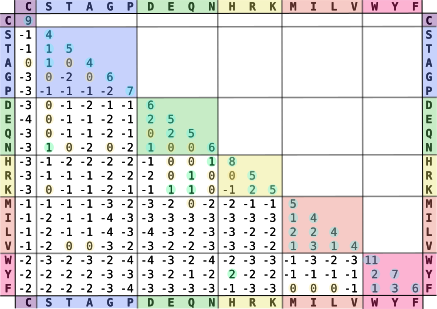
\includegraphics[width=0.7\linewidth]{figuras/blosum62-dayhoff} 

}

\caption{Matriz de sustitución aminoacídica BLOSUM62. Las letras en filas y columnas de la matriz refieren a los veinte aminoácidos naturales codificados directamente, y su color refleja sus tipos estructurales y fisicoquímicos. Las entradas numéricas de la matriz son proporcionales al logaritmo de la frecuencia con la que se observa la sustitución de un aminoácido por otro en proteinas homólogas. Valores positivos denotan mayores frecuencias de sustitución; lo contrario ocurre para valores negativos. Figura tomada de Wikipedia (CC BY-SA 3.0), versión original del archivo ``Blosum62-dayhoff-ordering.svg''}\label{fig:matrizblosum}
\end{figure}

Por ejemplo, mientras que en el caso de \textbf{\emph{Phe}} con \textbf{\emph{Tyr}} no hay diferencias en el contenido GC de los codones
implicados, en el segundo caso (\textbf{\emph{Ile}} con \textbf{\emph{Val}}) se trata del cambio A\(\leftrightarrow\)G en
primera posición del codón y por lo tanto estará sujeto a cambio cuando
el sesgo mutacional sea hacia GC (AT). Otros casos de cambios
relativamente frecuentes incluyen \textbf{\emph{Asp}} con \textbf{\emph{Glu}}, \textbf{\emph{Glu}} con
\textbf{\emph{Gln}}, \textbf{\emph{Ile}} con \textbf{\emph{Leu}}, \textbf{\emph{Arg}} con \textbf{\emph{Lys}}, \textbf{\emph{Leu}}
con \textbf{\emph{Met}}, \textbf{\emph{His}} con \textbf{\emph{Tyr}} y \textbf{\emph{Trp}} con \textbf{\emph{Tyr}}. De
todos estos solo el último implica un cambio de dos bases, el resto de
solo una base y casi todos independientes del contenido GC (de todos
estos solo \textbf{\emph{His}} con \textbf{\emph{Tyr}} implica cambio de GC). Esto podría
estar relacionado con un fuerte proceso selectivo para la optimización
de la estructura del código genético (\citeproc{ref-Novozhilov_Wolf_Koonin_2007}{Novozhilov, Wolf, and Koonin 2007}),
aunque existen teorías alternativas.

Bajando un poco más el nivel de
conservación (pero aún con ``\emph{score}'' positivo en la matriz BLOSUM62)
tenemos varios cambios que requieren cambio de contenido GC en los
codones implicados.

Un recurso extremadamente útil para comparar las propiedades de los
aminoácidos, así como para trabajar a partir de las mismas, es la
``AAindex database'' (\url{http://www.genome.jp/aaindex/})
(\citeproc{ref-Kawashima_Ogata_Kanehisa_2000}{Kawashima, Ogata, and Kanehisa 2000}). En la misma se encuentra registrada
información para unas 500 propiedades diferentes, así como información
adicional acerca de los autores, la publicación original y otras
auxiliares. La posibilidad de acceder a estas propiedades a través de la
biblioteca \emph{seqinr} de \emph{R} facilita enormemente la exploración de
hipótesis más complejas que se relacionen con la substitución de AAs
(ver por ejemplo (\citeproc{ref-Spangenberg_Battke_Grana_Nieselt_Naya_2011}{L. Spangenberg et al. 2011})).

\subsection*{Diferencias de composición entre clases de proteínas}\label{diferencias-de-composiciuxf3n-entre-clases-de-proteuxednas}
\addcontentsline{toc}{subsection}{Diferencias de composición entre clases de proteínas}

Existen diferentes clases de proteínas de acuerdo al criterio que se
utilice para clasificarlas y, en general, de acuerdo al criterio usado
poseen una composición diferente. Por ejemplo, de acuerdo a la forma
podemos clasificarlas en ``\emph{Fibrosas}'', ``\emph{Globulares}'' y ``\emph{Mixtas}''. Las fibrosas
presentan largas cadenas polipeptídicas, estructura secundaria atípica,
son insolubles en agua y en disoluciones acuosas (\emph{\href{http://v.gr/}{v.gr}.}, queratina,
colágeno y fibrina). Las globulares pliegan sus cadenas en una forma
esférica apretada, con los grupos hidrófobos hacia el interior y grupos
hidrófilos hacia afuera. Esto hace las mismas sean solubles en
disolventes polares como el agua. Entre ellas se encuentran los
anticuerpos, las enzimas, algunas hormonas y proteínas de transporte.
Finalmente, las mixtas poseen una parte fibrilar y otra parte globular.

Las proteínas solubles en agua suelen poseer los residuos hidrofóbicos
(\textbf{\emph{Leu}}, \textbf{\emph{Ile}}, \textbf{\emph{Val}}, \textbf{\emph{Phe}} y \textbf{\emph{Trp}}) escondidos
en el medio de la proteína (en su estructura), mientras que los
hidrofílicos se encuentran expuestos en la superficie. Al mismo tiempo,
las proteínas de membrana (IMPs) suelen contar con anillos externos
hidrofóbicos, los cuales sirven de anclaje en la bicapa lipídica. Por
otro lado, proteínas que deben interactuar con moléculas de carga
positiva suelen tener residuos de carga negativa en su superficie
(\textbf{\emph{Glu}} y \textbf{\emph{Asp}}) y viceversa (\textbf{\emph{Arg}} y \textbf{\emph{Lys}}). Algunos AAs
poseen propiedades muy particulares, con un efecto sustancial en la
estructura de la proteína. \textbf{\emph{Pro}} por ejemplo, que forma codos en la
estructura y \textbf{\emph{Cys}}, que forma puentes di-sulfuro estabilizando
estructuras.

Un grupo de particular interés son las proteínas de membrana, que
juegan un papel muy importante en el intercambio de moléculas entre la
célula y el exterior, así como en la transducción de señales. Por esta
razón es muy importante poder predecir qué secuencias se corresponden a
IMPs. Existen básicamente dos tipos de IMPs, las de \(\alpha\)-hélices
(TMH) y las de barriles-\(\beta\) (TMB). Las primeras se encuentran en la
membranas internas bacterianas y en las membranas plasmáticas
bacterianas, aunque a veces también en membrana externa. Es la mayor
categoría de proteínas transmembrana y una parte importante de todas las
proteínas humanas. Las proteínas de conformación tipo barriles-\(\beta\)
se encuentran solo en membrana externa de bacterias Gram-negativas,
pared celular de Gram-positivas y membrana externa de organelos.

Aunque existen distintos algoritmos y programas, la predicción de la
pertenencia a alguna de estas dos clases se basa esencialmente en el
mismo paradigma, básicamente el alineamiento a otras proteínas o
estructuras conocidas (\citeproc{ref-Bigelow_Rost_2009}{Bigelow and Rost 2009}). Un concepto clave en este
sentido es el de ``transferencia de homología a través de alineamientos''.
Bajo este paradigma, dos proteínas homólogas poseerán un alineamiento razonable. Por lo tanto, es posible transferir información derivada de evidencia experimental de una proteína a otra de interés para la que no se posee información. Claramente la capacidad de extender
las conclusiones depende de la calidad del alineamiento. Ejemplo de esto
serían regiones transmembrana en proteínas TMH: existen métodos
específicos para la predicción de ambas clases de IMPs. Los métodos
para detección de TMHs se basan en la presencia de una o más hélices
transmembrana. Dentro de estos métodos se encuentra \emph{TMHMM}
(\url{http://www.cbs.dtu.dk/services/TMHMM/}).

Entre los programas que permiten discriminar entre proteínas TMB o no-TMB se encuentra
\emph{TMB-Hunt}, que utiliza un algoritmo k-Nearest Neighbour (k-NN) sobre la
composición aminoacídica de las proteínas. El mismo permite además
incluir pesos diferenciales para los aminoácidos, así como información
evolutiva, lo que consigue una precisión mayor al 92\% con una
sensibilidad mayor al 91\% (\citeproc{ref-Garrow_Agnew_Westhead_2005}{Garrow, Agnew, and Westhead 2005}). Finalmente, una
alternativa interesante es utilizar \emph{InterScanPro}
(\url{http://www.ebi.ac.uk/Tools/pfa/iprscan/}), una herramienta que combina
la información de hasta 14 programas de predicción diferentes. Los
programas que se pueden seleccionar a través de esta herramienta son:
\emph{BlastProDom} (busca en la base de dominios \emph{ProDom}), \emph{FPrintScan}
(busca en la base \emph{PRINTS} de grupos de motivos), \emph{HMMPIR} (busca en
modelos HMM de la Protein Sequence Database, \emph{PSD}), \emph{HMMPfam} (busca en
modelos HMM de la base \emph{PFAM}), \emph{HMMSmart} (busca en modelos HMM de la
base \emph{SMART}), \emph{HMMTigr} (busca en modelos HMM de la base \emph{TIGRFAMs}),
\emph{ProfileScan} (busca contra perfiles de \emph{PROSITE}), \emph{HAMAP} (busca
contra perfiles de \emph{HAMAP}), \emph{PatternScan} (nueva versión de búsqueda
sobre \emph{PROSITE}), \emph{SuperFamily}, \emph{SignalPHMM}, \emph{TMHMM}, \emph{HMMPanther} y
\emph{Gene3D}. El costo computacional de estas búsquedas es muy elevado, y por
lo tanto se debe ser muy cauteloso a la hora de enviar varios trabajos
simultáneamente.

\subsection*{Ejemplo 1.4}\label{ejemplo-1.4}
\addcontentsline{toc}{subsection}{Ejemplo 1.4}

\emph{Escherichia coli} es una bacteria común en el intestino de los mamíferos. En la misma, el regulón del fosfato comprende un conjunto de más de 20 genes no-ligados cuyos promotores pueden ser regulados simultáneamente por controles superpuestos y separados. En particular, Los genes \textbf{phoS}, \textbf{phoA} y \textbf{phoE} son inducidos por la privación de fosfato y están sujetos a un control positivo por el producto del gen \textbf{phoB} y a un control negativo por el producto del gen \textbf{phoR}. Por otra parte, el sistema de transporte específico de fosfato (Pst) está codificado por cuatro genes estrechamente relacionados entre sí y situados juntos: \textbf{phoS}, \textbf{phoT}, \textbf{pstA} y \textbf{pstB}.

La siguiente es la secuencia de aminoácidos correspondientes al gen \textbf{pstA}, un transportador integral de membrana (Accesion K01992 del GenBank):

``MAMVEMQTTAALAESRRKMQARRRLKNRIALTLSMATMAFGLFWLI \newline
WILMSTITRGIDGMSLALFTEMTPPPNTEGGGLANALAGSGLLILW \newline
ATVFGTPLGIMAGIYLAEYGRKSWLAEVIRFINDILLSAPSIVVGL \newline
FVYTIVVAQMEHFSGWAGVIALALLQVPIVIRTTENMLKLVPYSLR \newline
EAAYALGTPKWKMISAITLKASVSGIMTGILLAIARIAGETAPLLF \newline
TALSNQFWSTDMMQPIANLPVTIFKFAMSPFAEWQQLAWAGVLIIT \newline
LCVLLLNILARVVFAKNKHG''

Si realizamos el análisis composicional de la misma llegamos la siguiente tabla:

\begin{table}
\centering
\begin{tabular}[t]{rrrrrrrrrrrrrrrrrrrr}
\toprule
A & C & D & E & F & G & H & I & K & L & M & N & P & Q & R & S & T & V & W & Y\\
\midrule
\cellcolor{gray!10}{38} & \cellcolor{gray!10}{1} & \cellcolor{gray!10}{3} & \cellcolor{gray!10}{11} & \cellcolor{gray!10}{13} & \cellcolor{gray!10}{21} & \cellcolor{gray!10}{2} & \cellcolor{gray!10}{27} & \cellcolor{gray!10}{10} & \cellcolor{gray!10}{41} & \cellcolor{gray!10}{17} & \cellcolor{gray!10}{9} & \cellcolor{gray!10}{12} & \cellcolor{gray!10}{8} & \cellcolor{gray!10}{13} & \cellcolor{gray!10}{16} & \cellcolor{gray!10}{22} & \cellcolor{gray!10}{18} & \cellcolor{gray!10}{9} & \cellcolor{gray!10}{5}\\
\bottomrule
\end{tabular}
\end{table}

El largo total es de \(296\) aminoácidos. La suma de los 4 aminoácidos hidrofóbicos más importantes (\textbf{A}, \textbf{I}, \textbf{L} y \textbf{V}) es de \(38+27+41+18=124\), es decir, \(\frac{124}{296}=41,9\%\) del total de aminoácidos. Si bien la comparación tiene poco sentido si no conocemos la composición global del genoma (es decir, del resto de las proteínas del genoma), sin duda es una buena pista de que se trata de una proteína de membrana (donde los aminoácidos hidrofóbicos juegan un papel relevante debido a la naturaleza lipídica de la bicapa que forma la membrana).

\begin{graybox}

\begin{itemize}
\tightlist
\item
  A nivel genómico la evolución se da por un conjunto de eventos como las mutaciones puntuales, las duplicaciones de genes y regiones o las inserciones y ``deleciones'' de secuencias nucleotídicas. El estudio de las variaciones en la composición de los genomas es lo que se puede llamar \textbf{genómica composicional} y forma parte de la \textbf{genómica comparativa}.
\item
  La idea del \textbf{análisis de correspondencia} es que dada una tabla de \(n \times p\) (casos x
  variables) encontrar un sistema de \(k\) ejes ortogonales (con \(k < min(n,p)\)) que condense el máximo de variación en los datos originales. \textbf{Esto es posible en la medida en que las variables (casos) estén correlacionados en alguna medida} y cuanto mayor sea esa asociación más varianza será condensada en pocos ejes (dimensiones).
\item
  La métrica adoptada en el \textbf{COA} es la de la distancia \(\chi^2\), o sea, para la celda correspondiente a la fila \(i\) y columna \(j\), la distancia será \(d_{ij}=(O_{ij}-E_{ij})^2/E_{ij}\) donde \(O_{ij}\) es el número observado y \(E_{ij}\) el número esperado para esa celda, usualmente el número total de observaciones multiplicado por las frecuencias relativas marginales en la tabla. El punto importante es determinar con cuantos ejes (nuevas dimensiones) nos vamos a quedar. Cuantas más dimensiones retengamos mayor cantidad de la varianza original retendremos, pero al costo de dificultar la interpretación.
\item
  Desde el punto de vista biológico, lo relevante del \textbf{COA}, además de identificar si podemos condensar la varianza en pocos ejes, es poder \textbf{etiquetar} cada eje con uno o unos pocos factores biológicos relevantes, tanto sean composicionales, de estructura del código, ambientales, etc.
\item
  Los distintos aminoácidos poseen diferentes propiedades que permiten agruparlos en diversos grupos, de acuerdo a las mismas. Por ejemplo, tenemos aminoácidos polares, apolares, hidrofílicos, hidrofóbicos, pequeños, medianos y grandes, alifáticos y aromáticos, etc. La importancia de esto es que permiten generar proteínas con diferentes propiedades y estructura tridimensional.
\item
  La redundancia en el código genético permite que un mismo aminoácido sea codificado por diferentes codones. Entre otras cosas, eso permite una mayor tolerancia a las mutaciones, ya que mutaciones que cambian el codon pero no el aminoácido no suelen tener mayor impacto en la estructura de la proteína (aunque puede ocurrir esto último debido a diferencias en la velocidad de traducción y su impacto en el plegamiento de la proteína).
\item
  El contenido G+C de los genomas es una variable extremadamente importante ya que se encuentra directamente asociada, entre otras cosas, a la composición de las proteínas. Diferentes hipótesis se han propuesto para explicar la enorme variabilidad entre los procariotas (\(20\%-80\%\)), pero en esencia se dividen en \textbf{neutralistas} y \textbf{seleccionistas}.
\end{itemize}

\end{graybox}

\section{Genómica comparativa}\label{genuxf3mica-comparativa}

Como vimos más arriba, solo es posible entender la biología de los
organismos si entendemos los procesos evolutivos subyacentes
(\citeproc{ref-Dobzhansky_1964}{Dobzhansky 1964}). De hecho, pese a que nuestra visión antropocéntrica
nos incline a vernos sustancialmente diferente de otras especies, desde
el punto de vista genómico compartimos una enorme similaridad con otras
especies. A nivel genómico la similitud nucleotídica es mayor al 98\% en
algunos casos, como por ejemplo con el chimpancé (\emph{Pan troglodytes})
(\citeproc{ref-Sequencing_Consortium_2005}{Sequencing and Consortium 2005}). Las diferencias que observamos entre las
especies pueden, en general, correlacionarse con diferencias a nivel
genómico, tanto por la presencia/ausencia de genes así como diferencias
en las secuencias que producen proteínas con diferencias
estructurales/funcionales o modificaciones en las redes regulatorias. La
genómica comparativa trata precisamente de identificar diferencias en
los genomas, entender los procesos evolutivos que llevan a esas
diferencias y en algunos casos de correlacionar estas diferencias con el
fenotipo o aún el ambiente donde se desarrollan los organismos.\\

\subsection*{Comparación de secuencias génicas}\label{comparaciuxf3n-de-secuencias-guxe9nicas}
\addcontentsline{toc}{subsection}{Comparación de secuencias génicas}

La base de la genómica comparativa se encuentra en la determinación de
homología en secuencias, es decir la inferencia sobre el origen
ancestral compartido de las mismas. En especial, la determinación de la
relación de ortología (ancestría común por especiación, ver nota al pie más arriba)
juega un papel central en la genómica comparativa ya que suele implicar
(aunque no siempre) la realización de la misma función en diferentes
organismos. La determinación de ortología es un problema usualmente
complejo, particularmente cuando hay varias especies implicadas. La base
de este proceso es la identificación de secuencias, en todas las
especies de interés, que presenten un nivel de similaridad tal que
permita inferir la relación de ortología. Debido a que es usualmente
necesario explorar muchos pares (solo la comparación de dos bacterias
requiere del orden de \(10^7\) comparaciones), se requiere de herramientas
que identifiquen similaridad rápidamente, lo que lleva al tipo de
alineamientos heurísticos como el del programa \emph{BLAST}.

Usualmente las secuencias ortólogas son las más similares en las otras especies. Esto ha llevado
al criterio práctico del \emph{Reciprocal Best Hit (RBH)}: un par de
secuencias se consideran ortólogas si cada una de ellas es la mejor
``selección'' (la más similar) en su correspondiente genoma, de la otra.
Un criterio de este tipo es necesario para evitar relaciones confusas
debido a la existencia de parálogos\footnote{Se dice que dos secuencias son parálogas si son producto de una duplicación ancestral. Un caso clásico para ilustrar este concepto es el de la familia de las hemoglobinas. Existen genes codificantes para \(\alpha\) y \(\beta\)-hemoglobina en humano y chimpancé, y se ha inferido que estos genes también existían en el ancestro común a ambas especies. Los genes de \(\alpha\)-hemoglobina y los de \(\beta\)-hemoglobina de las especies son ortólogas entre sí. Sin embargo, diríamos que la \(\alpha\)-hemoglobina de humano es paráloga a la \(\beta\)-hemoglobina de chimpancé, ya que su ``parentesco'' no se debe al proceso de especiación, si no a la duplicación del gen codificante para la hemoglobina ancestral.}. Cuando se comparan dos especies
este criterio está suficientemente bien definido; sin embargo, cuando se
trata de más de dos especies la existencia de parálogos en alguna de
ellas puede llevar a identificar distintas secuencias como pertenecientes
al grupo de ortólogas en dicha especie de acuerdo a qué pares de
especies se tomen en cuenta.

Este problema nos lleva a otros dos criterios de utilidad práctica a la
hora de identificar ortólogos. Por un lado, cuando la similaridad entre
secuencias es debida a eventos de especiación (definición de ortólogos,
ver más arriba) el orden de los distintos genes dentro del genoma será
relativamente similar durante mucho tiempo. Esto se debe a que los
re-arreglos genómicos suelen tener un importante costo evolutivo; en
procariotas en particular existen estructuras llamadas operones, que
facilitan la expresión coordinada de un conjunto de genes cuyos
productos interactúan directamente y que tienden a conservarse en la
evolución. Este ordenamiento puede ser usado para determinar las
relaciones de ortología, ya que además del alto nivel de identidad de
las secuencias podemos requerir que los genes en el vecindario de ambas
especies sean los mismos y estén ordenados de similar manera. Todo esto
es altamente dependiente de la distancia evolutiva entre los organismos
considerados, ya que a mayor tiempo de divergencia menos conservación de
estos patrones podemos esperar.

La otra aproximación, conocida como
\emph{filogenómica}, implica una cuidadosa reconstrucción filogenética\footnote{Una filogenia representa la historia evolutiva inferida para un conjunto de diferentes entidades, incluyendo patrones de ancestría y las tasas de cambio que llevaron a la diversidad observada. Si bien el ejemplo más paradigmático puede ser el de una filogenia de especies (donde se representa la evolución del grupo) también es posible pensar en una filogenia de genes o cualquier otra entidad autoreplicante que se modifique a lo largo del tiempo.}, a
partir de la cual se intenta conciliar los resultados del alineamientos
de las secuencias homólogas. Con un poco de suerte es posible determinar
correctamente las relaciones de ortología y paralogía de nuestras
secuencias. Los resultados obtenidos son altamente dependientes de la
reconstrucción filogenética, por lo que es necesario tener mucho cuidado
en la selección de secuencias para realizar la misma, en la correcta
selección del modelo de substitución (tanto aminoácidica como
nucleotídica) y el algoritmo de reconstrucción filogenética. En la medida de lo posible, es bueno explorar la sensibilidad
del análisis frente a posibles cambios en el proceso (por ejemplo la
selección de otro método de reconstrucción).

Existe una gran cantidad de software específico para atacar el problema
de la detección y determinación de ortólogos, así como bases de datos
para distintos grupos filogenéticos. Entre estas últimas podemos
destacar \emph{COG} (Cluster of Orthologous Groups,
\url{http://www.ncbi.nlm.nih.gov/COG/}), una base de datos construida a
partir de RBH con consistencia en al menos tres linajes para procariotas
y su extensión eucariótica \emph{KOG}, así como \emph{EGO}
(\url{http://compbio.dfci.harvard.edu/tgi/ego/}) una base de ortólogos para
eucariotas. Entre los programas podemos mencionar \emph{Inparanoid}
(\url{http://inparanoid.sbc.su.se/}) que consiste en RBH seguido de
agrupamiento de in-parálogos (parálogos dentro de una especie), así como
\emph{OrthoMCL} (\url{http://www.orthomcl.org/}) que a diferencia del primero usa
\textbf{E-value} y porcentaje de identidad para asignar las proteínas a
diferentes agrupamientos. Finalmente, un programa muy interesantes es
\emph{Orthostrapper} (\url{http://sonnhammer.sbc.su.se/download/software/}), y su
visualizador \emph{OrthoGUI}, que permite obtener valores de soporte
estadístico para la ortología de cada par de secuencias en un
alineamiento.

\subsection*{Selección positiva}\label{selecciuxf3n-positiva}
\addcontentsline{toc}{subsection}{Selección positiva}

Otro ejemplo interesante de las posibilidades de la genómica comparativa
es la determinación de sitios en el genoma (o genes) que se encuentran
evolucionando bajo selección positiva, o dicho en otras palabras, donde
la selección se orienta hacia una adaptación a un ambiente particular
(mejora en el ``\emph{fitness}''). Existen diversas formas de estudiar el efecto
de la selección a nivel molecular, pero uno de los usualmente más
aceptados es el de la relación \(\frac{K_a}{K_s}\) (también conocida como \(\omega\), o
dN/dS). Esta es la relación entre el número de substituciones no-sinónimas por
sitio no-sinónimo con respecto al número de substituciones sinónimas por
sitio sinónimo. Como las substituciones sinónimas es de esperar que sean
encontradas a una tasa usualmente mucho más alta que las no-sinónimas (ya que no generan cambios aminoacídicos y por lo tanto no repercuten en la función proteica),
aquellos sitios con una relación \(\frac{K_a}{K_s} > 1\) se consideran
bajo selección positiva. El problema principal radica en determinar
cuales apartamientos del 1 resultan estadísticamente significativos.

Existen diferentes formas de estimar \(K_a\) y \(K_s\), los más complejos usando
estimación por máxima-verosimilitud\footnote{Dado un modelo probabilístico, la estimación de parámetros por máxima-verosimilitud es un método que busca estimar los valores que maximizan la posibilidad de observar un conjunto de datos dado según el modelo.}, pero un método aproximado suele dar
resultados equivalentes cuando los datos son suficientes. En esencia, en
el método aproximado, a partir de un alineamiento de secuencias, se
realiza el conteo de sustituciones sinónimas y no-sinónimas, con
corrección por substituciones múltiples, para luego calcular la relación
\(\frac{K_a}{K_s}\). Es importante tener en cuenta que el alineamiento debe realizarse
a nivel de aminoácidos, para luego realizar el traducción reversa a
nucleótidos, asegurándose de esta forma que la comparación se realiza
codón a codón. Dentro del software clásico para estimar esta relación
podemos mencionar \emph{PAML}
(\url{http://abacus.gene.ucl.ac.uk/software/paml.html}) que realiza la
estimación por máxima-verosimilitud, mientras que entre las fáciles de
usar podemos mencionar la función \emph{KaKs} de la biblioteca \emph{seqinr} de
\emph{R}.

\subsection*{Vías}\label{vuxedas}
\addcontentsline{toc}{subsection}{Vías}

Las proteínas suelen realizar sus funciones particulares como partes de
procesos más complejos, que envuelven otras proteínas, en diferentes
etapas de esos procesos. El conjunto de proteínas (u otras móleculas)
que participan en un determinado proceso se conocen como vía. A modo de ejemplo podemos recordar la vía de la pentosas fosfato, durante la cual se utiliza la
glucosa para generar ribosa y poder reductor a través de NADPH. Las
distintas vías existentes en cada organismo se constituyen en el ``mapa''
de los distintos procesos biológicos que cada organismo es capaz de
realizar. Si bien el número de organismos donde todos los procesos
bioquímicos son conocidos al detalle es relativamente escaso, la
genómica comparativa es una alternativa importante para determinar la
capacidad de realización de distintos procesos en otros organismos.

La idea central en esta estrategia consiste en ubicar en el genoma de
interés ortólogos de los genes que constituyen una vía en un organismo
modelo, como puede ser \emph{E. coli}. Asumiendo que los genes ortólogos
posean aún la misma función, la completitud de la vía (es decir, la
presencia en el organismo de interés de todos los genes que la
constituyen en el modelo) permite inferir la capacidad de realizar el
proceso bioquímicos en el organismo de interés. Existen diferentes bases
de datos con representaciones de las diferentes vías en varios
organismos, pero probablemente la más conocida es \emph{KEGG Pathway}
(\url{http://www.genome.jp/kegg/pathway.html}). La misma permite la búsqueda
por diferentes criterios, posee información de varios organismos,
muestra la información en forma gráfica y existe una API (\emph{Application
Programming Interface}) que facilita el acceso a los datos a través de
software.

Por otro lado, la existencia de información de las diferentes vías puede
ser usada durante el proceso de anotación genómica, ya que si conocemos
que un organismo realiza determinado proceso bioquímico entonces deben
estar presentes todos los genes que constituyen esa vía. Si bien en
algunos organismos las vías pueden estar formadas por diferentes genes,
en general es posible determinar la falta de genes claves en las
distintas vías, lo que usualmente se debe a errores en el proceso de
anotación o a cambios desconocidos en las vías (esto último de gran
interés científico).

\begin{graybox}

\begin{itemize}
\tightlist
\item
  La \textbf{genómica comparativa} trata de identificar diferencias en los genomas, entender los procesos evolutivos que llevan a esas diferencias y en algunos casos de correlacionar estas diferencias con el fenotipo o aún el ambiente donde se desarrollan los organismos.
\item
  La base de la genómica comparativa se encuentra en la determinación de homología en secuencias, es decir la inferencia sobre el origen ancestral compartido de las mismas. En especial, la determinación de la relación de ortología (ancestría común por especiación, ver más arriba) juega un papel central en la genómica comparativa ya que suele implicar (aunque no siempre) la realización de la misma función en diferentes organismos. Usualmente las secuencias ortólogas son las más similares en las otras especies y esto ha llevado al criterio práctico del \textbf{Reciprocal Best Hit (RBH)}, es decir, un par de secuencias se consideran ortólogas si cada una de ellas es la mejor ``selección'' (la más similar) en su correspondiente genoma, de la otra. Cuando la similaridad entre secuencias es debida a eventos de especiación el orden de los distintos genes dentro del genoma será relativamente similara durante mucho tiempo.
\item
  La aproximación \textbf{filogenómica}, implica una cuidadosa reconstrucción filogenética, a partir de la cual se intenta conciliar los resultados del alineamientos de las secuencias homólogas. Los resultados obtenidos son altamente dependientes de la reconstrucción filogenética, por lo que es necesario tener mucho cuidado en la selección de secuencias para realizar la misma, en la correcta selección del modelo de substitución (tanto aminoácidica como nucleotídica) y el algoritmo de reconstrucción filogenética.
\item
  Existen diversas formas de estudiar el \textbf{efecto de la selección a nivel molecular}, pero uno de los usualmente más aceptados es el de la relación \(K_a/K_s\), que es la relación entre el número de substituciones no-sinónimas por sitio no-sinónimo con respecto al número de substituciones sinónimas por sitio sinónimo. Como las substituciones sinónimas es de esperar que sean encontradas a una tasa usualmente mucho más alta que las no-sinónimas, \textbf{aquellos sitios con una relación \(K_a/K_s\) por encima de 1 se consideran bajo selección positiva}. El problema principal radica en determinar cuales apartamientos del 1 resultan estadísticamente significativos.
\end{itemize}

\end{graybox}

\section{Genómica funcional}\label{genuxf3mica-funcional}

Las proteínas son los principales efectores a nivel celular (\emph{e.g.}, las enzimas), así como también juegan un rol fundamental en las estructuras celulares y las diferentes maquinarias, por lo que si intentamos entender el funcionamiento de células y tejidos a este nivel es necesario conocer cuándo, cuánto y dónde se producen. Por ejemplo, si queremos ver las diferencias entre un tejido determinado en estado normal y en el mismo tejido pero con un tumor, podríamos medir el nivel de cada proteína en ambos tejidos y comparar luego los niveles correspondientes para entender las diferencias. Desafortunadamente, la medición de proteínas a escala masiva (lo que se conoce como \textbf{\emph{proteómica}}) es un tema aún relativamente en pañales, si bien existen cientos de estudios desarrollados a esta escala en diferentes especies. Se trata de técnicas caras y complejas, que no han experimentado aún una explosión similar a la que se experimentó a nivel de la medición de ácidos nucleicos.

De acuerdo a una versión esquemática del paradigma de la biología molecular (paradigma que imperó durante muchos años), la información se almacena en el ADN, la que luego es transcrita hacia el ARN y que luego se traduce en proteínas. Si juntamos esto con el hecho de que es relativamente sencillo medir cantidades de \textbf{ARN} en forma masiva (en realidad \textbf{ADNc}), la idea de utilizar la medición de los transcritos como un \textbf{\emph{proxy}} a la medición de proteínas surge de inmediato. Es decir, si suponemos que la tasa de producción de proteínas es directamente proporcional a la tasa de transcripción, entonces medir la cantidad de transcritos es una buena y fiable indicación de la producción de proteínas (aunque existe una compresión de rango entre el logaritmo de la relación de proteínas y el logaritmo de la relación de mensajeros, como lo muestran L. Spangenberg et al. (\citeproc{ref-Spangenbergetal2013}{2013})). Claramente, a pesar de su enorme importancia en el desarrollo de la disciplina, esta visión simplificada del paradigma de la biología molecular ha sido ampliamente sobrepasada por la información generada en los últimos años, incluyendo los descubrimientos de los microARNs y de un gran número de otros ARNs que juegan un papel fundamental en la regulación de la expresión génica. Más aún, la vida media de los diferentes transcritos no es necesariamente igual, lo que conlleva un error a la hora de utilizar su cantidad (no su tasa de producción) como indicador de la producción de proteínas.

A pesar de todos estos problemas, el análisis de la expresión de los \textbf{ARN mensajeros} (\textbf{ARNm}) sigue siendo la principal herramienta para entender los cambios a nivel de expresión en los distintos tipos de órganos y tejidos, así como en células bacterianas o de otras especies. En un principio, los \textbf{microarrays} fueron fundamentales para esta tarea ya que permitían interrogar miles de genes al mismo tiempo. Desde los originales \textbf{spot arrays} que eran impresos por un robot cartesiano mediante un bloque de agujas que depositaban las sondas en una placa de vidrio, diferentes tecnologías se fueron desarrollando. Una de las principales limitaciones de los primeros arrays era la necesidad de utilizar algún tipo de ``referencia'', es decir algo contra lo que contrastar las mediciones debido a las imperfecciones de las impresiones con agujas. Posiblemente de las tecnologías más conocida es la desarrollada por la empresa \textbf{Affymetrix} (fundada por el bioquímico uruguayo Alejandro Zaffaroni) que utilizando la misma tecnología que se utiliza para la fabricación de chips de semiconductores (esencialmente la fotolitografía) consiguieron desarrollar arrays de altísima densidad. La figura \ref{fig:affychips} muestras dos arrays de esta marca, a la izquierda un chip para genoma humano, mientras que a la derecha aparece un chip para genoma de ratón; en la parte inferior aparece un fósforo a efectos de imaginar el tamaño de los mismos. La principal ventaja de estos arrays respecto a los típicos \textbf{spotted} era la muy alta precisión con los que eran fabricados, lo que permitía evitar tener que usar una referencia. Sin embargo, el principal problema con estos arrays era el costo de desarrollo asociado a cada nuevo diseño, por lo que quedaron reducidos a las pocas especies que eran modelo para la investigación (humano, ratón, \emph{Arabidopsis thaliana}, etc.).



\begin{figure}[H]

{\centering 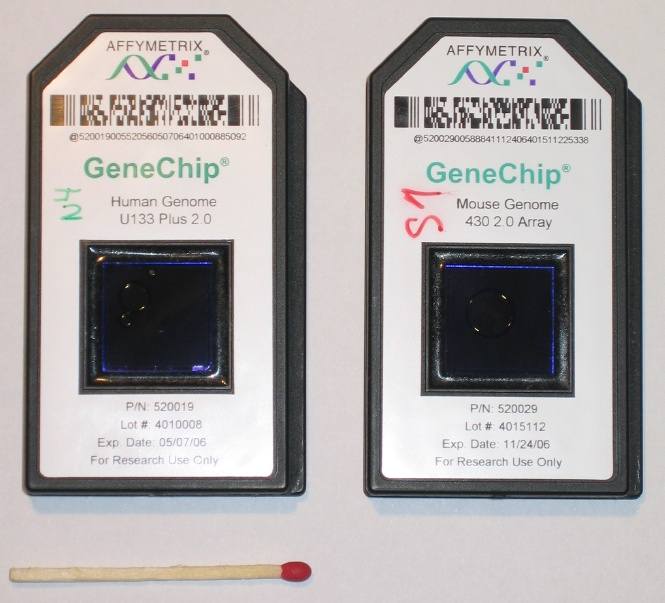
\includegraphics[width=0.5\linewidth]{figuras/Affymetrix-microarray} 

}

\caption{Dos \emph{chips} de Affymetrix, uno para genoma humano a la izquierda, el otro para genoma de ratón. El fósforo debajo es solo a fines de comparación del tamaño. La fecha de expiración de ambos es en el año 2006, por lo que su uso seguramente fue anterior (Schutz, trabajo propio (based on copyright claims)., CC BY 2.5, \url{https://commons.wikimedia.org/w/index.php?curid=694717}).}\label{fig:affychips}
\end{figure}

Un poco más tarde, la tecnología de la empresa \textbf{Agilent}, la \textbf{impresión laser} de los arrays permitió combinar una altísima precisión con la posibilidad de fabricar los mismos a gusto del consumidor y sin costos adicionales, lo que llevó a utilizarlos en decenas de nuevas especies. En efecto, en lugar de utilizar tinta de diferentes colores, el array se construía imprimiendo un nucleótido por vez en cada posición de una sonda, utilizando como tintas 4 soluciones con los nucleótidos A, C, G y T. La precisión de esta tecnología permitía realizar análisis en experimentos de un solo canal o en experimentos con dos canales, lo que en ciertos casos posibilitaba reducir los costos (por ejemplo, cuando existe una referencia natural para cada caso, utilizando el mismo array se elimina la necesidad de dos arrays).

Finalmente, en años recientes, las tecnologías de secuenciación masiva llegaron a este campo y mediante la secuenciación del \textbf{ARNc} permiten obtener una representación mucho más amplia y fidedigna de las proporciones de los distintos mensajeros. Además, como se obtienen las secuencias de los mismos, es posible identificar variantes (que son a su vez producto de variantes en el \textbf{ADN}) asociadas a cambios en la expresión entre individuos, lo que se conoce como \textbf{eQTL} (``expression Quantitative Trait Locus''). La principal diferencia entre el análisis de expresión con arrays respecto a la secuenciación (que se conoce como \textbf{RNA-seq}) es que en el primer caso la señal obtenida es analógica (un número en una escala continua), mientras que en el segundo caso es digital (en realidad el conteo de los reads que mapean a un transcrito particular).

La idea de las comparaciones es similar en las diferentes tecnologías, aunque cada tecnología requiere de detalles específicos a la hora de analizar los datos. En general, si vamos a comparar el perfil de expresión en dos tratamientos diferentes, por ejemplo tejido sano y tumoral, requerimos de varios individuos en cada tratamiento a fin de tener en cuenta la variación entre individuos y de que nuestras conclusiones se puedan extrapolar de alguna manera a la población general. Luego de haber obtenido los perfiles de expresión en cada individuo necesitamos realizar algún tipo de normalización, ya que las cantidades absolutas suelen depender de la preparación de las bibliotecas. Luego de normalizadas las muestras debemos comparar gen a gen, lo que suele hacerse mediante un modelo lineal sobre los datos transformados de alguna manera. En los casos en que se compara un tratamiento contra una referencia, se acostumbra a utilizar la distribución del logaritmo de la relación de cambio entre las dos condiciones (que se llama \(logFC\)). Es decir, si la expresión del gen \(i\) en el tratamiento es \(mRNA_{i,1}\) y en la referencia o control es \(mRNA_{i,2}\), entonces

\begin{equation}
logFC_i=log\left[\frac{mRNA_{i,1}}{mRNA_{i,2}}\right]
\label{eq:logfc1}
\end{equation}

Las ventajas de esta transformación son varias. Por un lado, tanto las distribuciones de conteo (en el caso de RNA-seq) como las de señal luminosa tienen una cola larga a la derecha, es decir, una serie de valores muy altos y alejados de donde se concentra la mayor parte de la distribución; el logaritmo ``corrige'' de alguna forma eso, transformándolas en distribuciones parecidas a la normal. En segundo caso, mientras que la relación \(\frac{mRNA_{i,1}}{mRNA_{i,2}}\) es asimétrica (cuando el numerador es más pequeño que el denominador la relación queda entre 0 y 1, mientras que al revés va de 1 a \(+\infty\)), la relación transformada \(log\left[\frac{mRNA_{i,1}}{mRNA_{i,2}}\right]\) es simétrica y centrada en cero, además de relativamente normal. Con esta transformación, por ejemplo si hay solo dos grupos a comparar, la comparación podría ser a través de un test de \(t\) (la distribución). Como realizamos miles de comparaciones a la vez (una por gen), la significación estadística de cada gen debe ajustarse para múltiples ensayos, lo que usualmente se realiza a través de algún método como Benjamini-Hochberg.

\subsection*{Estudios epigenéticos y epigenómicos}\label{estudios-epigenuxe9ticos-y-epigenuxf3micos}
\addcontentsline{toc}{subsection}{Estudios epigenéticos y epigenómicos}

Hasta ahora hemos manejado los aspectos de la genética que tienen que ver con la transmisión de información como algo bastante rígido y donde hay poco margen para cambiar lo recibido de los progenitores. Sin embargo, existen una serie de mecanismos que tienen que ver con la regulación que pueden transmitirse de padres a hijos y a su vez ser modificados posteriormente de recibidos. El estudio de estos mecanismos particulares es el objetivo de la epigenética y de la epigenómica. Básicamente, la epigenética se centra en los procesos que regulan la activación y desactivación de genes, tanto en lo que hace a cómo y cuándo se produce esto. Por otra parte, la epigenómica se refiere a los cambios globales que ocurren a nivel de genoma que permiten activar o desactivar un conjunto de genes, tanto a nivel de células como de organismos.

En general, los procesos epigenéticos son los responsables de controlar el crecimiento y desarrollo de un organismo. En situaciones particulares, la alteración del control puede llevar a procesos patogénicos, como por ejemplo el cáncer. Lo trascendente de este proceso es que factores ambientales pueden ser los causantes del desajuste en la regulación y por lo tanto en el desarrollo de patologías. Dentro de los factores ambientales conocidos, la exposición a determinadas sustancias químicas aparece como muy relevante, aunque también la dieta parece estar relacionada con alteraciones en la regulación. Además, existe cierta evidencia de los cambios en la regulación podrían ser transmisibles.

Existen dos formas en las que el epigenoma es capaz de marcar el ADN para la regulación génica: a) la metilación y b) la modificación de las histonas. En la primera, grupos metilo se intercalan en la molécula de ADN modificando la función cuando esto ocurre en un gen promotor. En general, la metilación del ADN actúa reprimiendo la transcripción génica. En mamíferos entre el \(60\%\) y el \(90\%\) de todas las CpG están metiladas. Por otra parte, en la segunda forma de acción una serie de modificaciones en las histonas (acetilación, metilación, desmetilación, fosforilación, ubiquitilación, etc.) modifican el arrollamiento del ADN y por lo tanto la disponibilidad para la transcripción.

Por supuesto, existen arrays disponibles para el estudio de las modificaciones epigenómicas, así como métodos para realizar los estudios a través de secuenciación masiva.

\begin{graybox}

\begin{itemize}
\tightlist
\item
  Las proteínas son los principales efectores a nivel celular, así como también juegan un rol fundamental en las estructuras celulares y las diferentes maquinarias, sin embargo, desafortunadamente, la medición de proteínas a escala masiva (lo que se conoce como \textbf{proteómica}) es un tema aún relativamente nuevo: se trata de técnicas ´aún caras y complejas y que no han experimentado aún una explosión similar a la que se experimentó a nivel de la medición de ácidos nucléicos.
\item
  Como sabemos, la información se almacena en el \textbf{ADN}, la que luego es transcrita hacia el \textbf{ARN} y que luego se traduce en proteínas. Si a su vez consideramos el hecho de que es relativamente sencillo medir cantidades de ARN en forma masiva (en realidad ADNc), la idea de utilizar la medición de los transcritos como un proxy a la medición de proteínas surge de inmediato. Es decir, \textbf{si suponemos que la tasa de producción de proteínas es directamente proporcional a la tasa de transcripción, entonces medir la cantidad de transcritos es una buena y fiable indicación de la producción de proteínas}.
\end{itemize}

\end{graybox}

\section{Conclusión}\label{conclusiuxf3n}

El estudio de la vida se ha nutrido a lo largo de los siglos del avance tecnológico; ejemplos claros de esto son la aparición del microscopio (que permitió vislumbrar que la vida habitaba lugares insospechados en formas diminutas) o los avances de la química, que permitieron comprender los mecanismos subyacentes al funcionamiento de la maquinaria celular y la herencia desde una perspectiva molecular. El uso de herramientas matemáticas también ha sido fundamental para el desarrollo teórico de la biología: pensemos en la importancia que tuvo la simple aproximación de Mendel al estudio de la herencia de caracteres.

No es de extrañar que en décadas marcadas por el avance de las ciencias de la informática y del procesamiento tecnológico de compuestos químicos también exista una nueva vigorización de nuestro entendimiento de la biología. En este capítulo presentamos varias de las áreas de estudio que han surgido o se han visto vitalizadas por la aparición de métodos de secuenciación masiva (\emph{i.e.,} las distintas áreas de la genómica), discutiendo su impacto en la tipificación y estudio de la diversidad genética, la identificación y análisis evolutivo de organismos o el análisis de la expresión génica y uso de codones.

En el resto del libro trataremos dos áreas sumamente importantes de la genética: el estudio de la herencia a nivel poblacional y el análisis cuantitativo. Las tecnologías y la forma de análisis que vimos en este capítulo reaparecerán constantemente a medida que aprendamos cómo se observa la genética a través de estas dos potentes lentes conceptuales. Antes de seguir con ese recorrido, es importante remarcar nuevamente que estas dos áreas surgieron mucho antes que las tecnologías que mencionamos en este capítulo: una vez más en la historia de la biología, la aparición de tecnologías da nuevos datos y perspectivas de análisis a marcos teóricos que ya existían, ayudando a testear hipótesis, ampliar nuestro conocimiento e impulsando nuevas preguntas sobre el fenómeno de la herencia.

\newpage

\section{Actividades}\label{actividades}

\subsection{Control de lectura}\label{control-de-lectura}

\begin{enumerate}
\def\labelenumi{\arabic{enumi}.}
\tightlist
\item
  Existen muchas maneras de medir la diversidad biológica. Mencione al menos una, explicitando la forma de cálculo y en qué contexto puede ser útil la medida elegida.
\item
  ¿Qué es un \emph{microarray}? Explique la utilidad de esta herramienta, poniendo algún ejemplo de su aplicación.
\item
  En las últimas décadas se han desarrollado un conjunto de disciplinas que permiten la obtención y análisis masivo de datos biológicos. Identifique el objeto de estudio de las siguientes:

  \begin{enumerate}
  \def\labelenumii{\arabic{enumii}.}
  \tightlist
  \item
    Genómica
  \item
    Transcriptómica
  \item
    Proteómica
  \item
    Metagenómica
  \item
    Metatranscriptómica
  \item
    Epigenómica
  \end{enumerate}
\item
  Actualmente se acepta que todos los organismos provenimos de un ancestro común (denominado LUCA). ¿Cómo se explica entonces que existan diferencias tan grandes entre los organismos vivos? Mencione al menos una aproximación para el estudio de esta diversidad biológica.
\item
  Defina el concepto de codón. ¿Todos los organismos usan el mismo conjunto de codones? ¿Los codones son todos usados en igual proporción?
\end{enumerate}

\subsection{¿Verdadero o falso?}\label{verdadero-o-falso}

\begin{enumerate}
\def\labelenumi{\arabic{enumi}.}
\tightlist
\item
  Un codón solo codifica para un aminoácido, pero un aminoácido puede estar codificado por más de un codón.
\item
  La estructura del código genético refleja las propiedades fisicoquímicas de los aminoácidos codificados en el llamado ``código genético universal''.
\item
  La secuenciación y comparación de secuencias de ARNr 16S permite la identificación y estudio filogenético de todos los organismos vivos.
\item
  El contenido GC de los organismos no es uniforme, existiendo variaciones a lo largo del árbol de la vida.
\item
  Todos los cambios genéticos heredables se encuentran codificados en el genoma de los organismos, por lo que secuenciando y comparando secuencias genéticas podemos comprender en su totalidad el proceso de herencia de información entre individuos (y en las poblaciones).
\end{enumerate}

\textbf{\emph{Solución}}

\begin{enumerate}
\def\labelenumi{\arabic{enumi}.}
\tightlist
\item
  \textbf{Verdadero}. Este concepto suele denominarse ``redundancia'' o ``degeneración'' del código genético. Entre otras cosas, eso permite una mayor tolerancia a las mutaciones, ya que mutaciones que cambian el codon pero no el aminoácido no suelen tener mayor impacto en la estructura de la proteína (aunque puede ocurrir esto último debido a diferencias en la velocidad de traducción y su impacto en el plegamiento de la proteína).
\item
  \textbf{Verdadero}. Los cambios sinónimos suelen llevar con más frecuencia a aminoácidos de características fisicoquímicas similares, hecho que podría adjudicarse a un régimen selectivo que favoreció el evitar que el proceso mutacional lleve a cambios radicales en las proteínas codificadas.
\item
  \textbf{Falso} Si bien es cierto que la secuenciación de ARN ribosomal es útil para identificar tanto a organismos procariotas como eucariotas, es importante recordar que las subunidades secuenciadas varían en los dominios de la vida: en procariotas si se recurre al estudio de la subunidad 16S, mientras que en eucariotas se recurre al 18S (recordar que no existe subunidad 16S en eucariotas).
\item
  \textbf{Verdadero}. El contenido de GC (o lo que es lo mismo, AT) varía ampliamente entre organismos. Ya en la década de 1960 se determinó que existen bacterias cuyo genoma se encuentra en un rango que va de 25 a 75\% de contenido GC. Tal es la diferencia, que en muchos casos es posible identificar transferencias de material genético entre diferentes especies bacterias observando que tramos del genoma desvían fuertemente de la tendencia general observada en el resto del genoma (se ahondará en este tema en el capítulo \hyperref[microbial]{Genética de Poblaciones Microbianas}).
\item
  \textbf{Falso}. Si bien este fue un paradigma dominante durante décadas, la existencia de transmisión de información epigenética (\emph{e.g.} a través de patrones de metilación y acetilación de histonas) muestra que es posible la herencia de información biológica que no se encuentra codificada a nivel nucleótidico. Disciplinas como la epigenómica intentan estudiar la relevancia de estos procesos en la herencia de los individuos e incluso la evolución.
\end{enumerate}

\subsection*{Ejercicios}\label{ejercicios-1}
\addcontentsline{toc}{subsection}{Ejercicios}


\includegraphics[width=0.06\textwidth,height=\textheight]{figuras/cienciabasica.png} \(\raisebox{2.5ex}{\textbf{Ejercicio 1.1}}\)

Dada la siguiente secuencia ``AUGGGAUUUCCGCCCAUUUACGUG''

\textbf{a.} Determinar de que ácido nucléico se trata (ADN o ARN).
\textbf{b.} Si tiene sentido traducirla a una secuencia de aminoácidos tomandola como hebra \textbf{codificante} y en marco de referencia.
\textbf{c.} Escribir en sentido 5'--\textgreater3' la hebra complementaria pero en ADN (hebra molde) d) calcular el contenido G+C.

\textbf{\emph{Solución}}

\textbf{a.} Se trata de ARN ya que entre sus bases aparece \textbf{U}racilo en lugar de \textbf{T}imina.

\textbf{b.} En principio parece tener sentido, por lo que asumiendo que está en marco de referencia correcto y y que se trata de la hebra codificante, separamos en codones ``AUG GGA UUU CCG CCC AUU UAC GUG'', que utilizando el código genético se traduce como MGFPPIYV.

\textbf{c.} ``CAC GTA AAT GGG CGG AAA TCC CAT''.

\textbf{d.} 6G + 6C= 12 G o C en un total de {[}8 codones x 3 bases c/u = 24 bases{]}, por lo tanto 12/24=0.5 o 50\%.

\hfill\break


\includegraphics[width=0.06\textwidth,height=\textheight]{figuras/cienciabasica.png} \(\raisebox{2.5ex}{\textbf{Ejercicio 1.2}}\)

Un investigador obtuvo la siguiente secuencia (según él) de un nuevo gen que sería responsable de la generación de radiactividad por parte de una especie bacteriana que lo posee (presentamos la secuencia ordenada en tripletes y en marco de lectura correcto, para mayor facilidad de visualización):

\begin{lstlisting}
GTC TCT CGT GAT GCG GTT GTC ATA AGA GCT GGC TCT GAG CTG
AAT TGA AGC ATA TCC TTC GCA GTC TTA AAA GGG TTG GGA TTA
TCA ACC TCC CAC GCA ATA CCG GCG TTC AAC AGT TTA CCA TCA
TCT ACT GAC GCG TGA TGT TGC GGA GCG ACG GGA AGT GAT
AAA AGT TAC TTT ACA
\end{lstlisting}

La especie bacteriana de la que supuestamente fue aislado el gen, posee un
contenido GC del 80 \%.

Por otra parte, un estudiante de su grupo afirma que no solamente no se trata
de la secuencia de un nuevo gen, sino que no se trata de la secuencia de ningún
gen. Más aún, plantea que esta secuencia fue generada en forma aleatoria por
una máquina y que posiblemente el investigador ha sido engañado por alguien.
El conteo de bases dio lo siguiente:

\[
\begin{cases}
A: 46 \\
C: 40 \\
G: 45 \\
T: 49
\end{cases}
\]

mientras que el conteo de aminoácidos fue el siguiente:

\[
\begin{cases}
STOP: 2 \\
A: 7 \\
C: 2 \\
D: 3 \\ 
E: 1 \\
F: 3 \\
G: 5 \\
H: 1 \\
I: 3 \\
K: 2 \\
L: 5 \\
N: 2 \\
P: 2 \\
R: 2 \\
S: 11 \\
T: 4 \\
V: 4 \\
Y: 1
\end{cases}
\]

\textbf{a.} ¿Quién de los dos parece tener razón? Argumenta las razones que te llevan
a esa conclusión.

\textbf{b.} ¿Cuántas cisteínas hay codificadas en la secuencia y dónde se encuentran?

\textbf{c.} ¿Cuántas serinas y cuántas argininas serían de esperar en una secuencia
de este largo si se tratase de una secuencia creada al azar y cuántas
fueron observadas? ¿Y la suma de las dos (es decir, para los codones de
los sextetos)?

\textbf{d.} Determinar mediante un test estadístico si el número de Serinas y de
Argininas observadas cae dentro de lo esperado, o si debemos rechazar
dicha hipótesis nula.

\textbf{\emph{Solución}}

\textbf{a.} Algunos hechos hacen sospechar que no se trata de una secuencia presente en un organismo vivo tal y como los conocemos:

\begin{itemize}
\tightlist
\item
  El codón de iniciación no es ATG ni tampoco ninguna de las formas alternativas más usuales (esta argumento no es excluyente, pero es raro de observar).
\item
  En la posición 46, es decir el inicio del codón 16, corresponde con el codón
  TGA que es un codón terminación, lo que nos dejaría con una proteína de 15
  aminoácidos de largo. Lo mismo ocurre en la posición 139, es decir el inicio del
  codón 47, por lo que tampoco parece mucho mejor la situación del fragmento
  interno entre ambos codones STOP.
\item
  La secuencia no termina en ninguno de los codones STOP conocidos.
\item
  La distribución de la frecuencia de bases no se aparta mucho de lo esperado para una secuencia obtenida al azar (\(\frac{180}{4} = 45\)). En cambio, si el contenido del genoma bacteriano fuese de \(80\%\), entonces esperaríamos \(180∗0,80 2 = 72\) bases para G y lo mismo para C, mientras que esperaríamos \(180∗0,20 2 = 18\) bases para A y lo mismo para T.
\end{itemize}

\textbf{b.} Dos cisteínas, y se encuentran codificadas por los codones 48 y 49.

\textbf{c.} La serina está codificada por 6 codones y Arginina por otros 6 codones, de los 64 que hay en el código genético, o lo que es lo mismo, de \(4^3 = 64\) posibles combinaciones de cada bases (A, C, G, T) en 3 posiciones. Como hay un total de 60 codones en la secuencia, esperamos: \(\text{Ser} = 60 ∗ \frac{6}{64} = 5,625\), \(\text{Arg} = 60 ∗ \frac{6}{64} = 5,625\). Se observaron 11 y 2 respectivamente, lo que en ambos casos parece algo alejado del esperado. Sin embargo, la suma de ambos sextetos da 13, mientras que el
esperado es \(\text{Ser}+\text{Arg} = 60 ∗ \frac{12}{64} = 11,25\), lo que parece mucho más cercano.

\textbf{d.} Un test de chi-cuadrado de ``goodness-of-fit'' (bondad de ajuste) podría ser adecuados en este caso.


\includegraphics[width=0.06\textwidth,height=\textheight]{figuras/cienciabasica.png} \(\raisebox{2.5ex}{\textbf{Ejercicio 1.3}}\)

\hfill\break

Observando la tabla con el código genético universal agrupar los aminoácidos
por el número de codones que los codifican y resumir el número de aminoácidos
con cada multiplicidad. ¿Qué característica comparten la mayor parte de los
duetos (los aminoácidos codificados por dos codones)?

\textbf{\emph{Solución}}

\begin{itemize}
\tightlist
\item
  1 codon: \textbf{Met}, \textbf{Trp}
\item
  2 codones: \textbf{Phe}, \textbf{Tyr}, \textbf{His}, \textbf{Gln}, \textbf{Asn}, \textbf{Lys}, \textbf{Asp}, \textbf{Glu}, \textbf{Cys}
\item
  3 codones: \textbf{Ile}
\item
  4 codones: \textbf{Val}, \textbf{Pro}, \textbf{Thr}, \textbf{Ala}, \textbf{Gly}
\item
  6 codones: \textbf{Leu}, \textbf{Arg}, \textbf{Ser}
\end{itemize}

La característica que comparten 7 de 9 duetos es que se encuentran en la tercer
columna de la tabla del código, es decir, tienen una A en segunda posición del
codon.

\hfill\break


\includegraphics[width=0.06\textwidth,height=\textheight]{figuras/cienciabasica.png} \(\raisebox{2.5ex}{\textbf{Ejercicio 1.4}}\)

En un planeta de otra galaxia existe vida con algunas similitudes a la que existe
en nuestro planeta. En particular, también las proteínas parecen ser la base
estructural y funcional de la vida, mientras que los ácidos nucléicos son los
responsables del mantenimiento y duplicación de la información. Sin embargo,
a diferencia de nuestro planeta, los aminoácidos proteinogénicos codificados son
24, mientras que las bases nucleótidicas análogas a las de nuestro ADN son 5.
Suponiendo que los mecanismos moleculares en dicho planeta han sido seleccionados para ser altamente eficientes

\textbf{a.} ¿De qué largo mínimo deberían ser los codones?

\textbf{b.} Si el código genético en ese planeta tuviese algún nivel de redundancia (más de un codón para el mismo aminoácido), ¿de qué largo mínimo serían los codones? En ese caso, ¿cuál sería el número promedio de codones por
aminoácido?

\textbf{c.} ¿Cómo se compara esa redundancia promedio con la existente en nuestro
planeta?

\textbf{d.} ¿Qué ventaja potencial tiene la redundancia en el código?

\textbf{\emph{Solución}}

\textbf{a.} Si existen 5 bases nucleotídicas y 24 aminoácidos, entonces con codones de
largo 2 tenemos \(5 \times 5 = 25\) combinaciones posibles. Si consideramos
la existencia de un codón \textbf{STOP}, entonces el mínimos es \(24 + 1 = 25\)
codones, por lo que alcanza con largo de codón 2.

\textbf{b.} Si queremos algo de redundancia vamos a precisar un código genético
con largo mayor a 2. El siguiente largo es 3, por lo que ahora tenemos
\(5 \times 5 \times 5 = 5^3 = 125\) codones.
Como hay \(24\) AAs \(+1\) \textbf{STOP} \(= 25\) ``necesidades'', entonces la redundancia
promedio será igual a \(\frac{125}{25} = 5\).

\textbf{c.} En nuestro planeta tenemos 20 aminoácidos proteinogénicos codificados
directamente, por lo que equivale a \(20\) AAs \(+1\) STOP = 21 ``necesidades''.
Sin embargo, al existir solo 4 bases nucleotídicas en nuestro código y el
largo de nuestros codones ser de 3, entonces tenemos un total de \(4 \times 4 \times 4 =
4^3 = 64\) posibilidades. Por lo tanto, en nuestro planeta, la redundancia
promedio es de \(\frac{64}{21} \approx 3,05\).

\textbf{d.} La redundancia en el código tiene como ventaja que es capaz de absorber
determinadas mutaciones (cambio de bases) sin cambiar el aminoácido
codificado, lo que lo hace un sistema con cierta robustez o tolerancia a los
fallos en la duplicación de la información (mutaciones).

\hfill\break


\includegraphics[width=0.06\textwidth,height=\textheight]{figuras/cienciabasica.png} \(\raisebox{2.5ex}{\textbf{Ejercicio 1.5}}\)

Asumiendo que existen 20 aminoácidos (los estándar),

\textbf{a.} ¿Cuántas proteínas diferentes de largo 5 aminoácidos sería posible tener?

\textbf{b.} Cuántas serían posibles de largo \(n\)?

\textbf{c.} Considerando que una proteína de largo promedio en procariotas es del
orden de los 300 aminoácidos, ¿cuántas proteínas diferentes, con ese largo
se podrían codificar?

\textbf{\emph{Solución}}

\textbf{a.} Se podrían codificar \(20 \times 20 \times 20 \times 20 \times 20 = 20^5 = 3,200,000\).

\textbf{b.} De largo \(n\) se pueden codificar \(20^n\).

\textbf{c.} En el caso de \(n = 300\), tenemos \(20^300 \approx \infty\) para los fines prácticos

\begin{center}\rule{0.5\linewidth}{0.5pt}\end{center}

\part*{Parte II: Genética de Poblaciones}\label{part-parte-ii-genuxe9tica-de-poblaciones}
\addcontentsline{toc}{part}{Parte II: Genética de Poblaciones}

\chapter{Variación y equilibrio de Hardy-Weinberg}\label{variacion}

Una de las características evidentes de la vida en nuestro planeta es la
heterogeneidad de los organismos, aún dentro del nivel taxonómico más
bajo que se nos ocurra para clasificarlos razonablemente (por ejemplo,
especie o sub-especie). Es decir, aún a simple vista podemos usualmente
distinguir esa ``falta de uniformidad'' como una de las características
\textbf{aparentemente} distintivas de los seres vivos. Pensemos esto en
contraposición con el resultado de los productos industriales, como
autos, lámparas LED, televisores, etcétera. Existe en estos objetos artificiales muchísima homogeneidad, más allá de que el uso de todas
estas cosas las transforma de alguna manera en únicas (en general luego
de un tiempo y más allá de la matrícula o el número de chasis, todos
somos capaces de reconocer nuestro propio vehículo, especialmente si en
el mismo viajan 4 niñas pequeñas). Como veremos y analizaremos más
adelante, el \textbf{\emph{fenotipo}}, aquello que podemos observar (usualmente a
simple vista en los organismos macroscópicos, luego veremos definiciones
más precisas) es el producto de la información contenida en el
\textbf{\emph{genotipo}} (la información genética, aunque veremos que esto no es muy
preciso dicho así) y de su interacción con el \textbf{ambiente}, que a los
efectos operacionales termina siendo todo lo no-genético.

La importancia de \emph{``lo genético''} en el fenotipo no deja lugar a dudas:
por un lado, los individuos ``similares'' se aparean entre ellos y no con
los ``distintos'' (tanto sea a nivel de especie, o sub-especie, por
ejemplo). Por otro lado, en un mismo ambiente co-existen individuos muy
distintos (\emph{i.e.}, individuos pertenecientes a especies diferentes), por
lo que el ambiente \emph{per se} no estaría determinando una gran parte de
los fenotipos. Pese a esta importancia de lo genético, entender los
mecanismos que están por detrás de este fenómeno fue un proceso largo y
complejo que recién pasada la mitad del siglo XX permitió elaborar una
teoría relativamente completa a los distintos niveles involucrados
(desde el nivel macro de los organismos, al nivel molecular del ADN,
pasando por los niveles de organización intermedia de la información y
sus formas de transferencia). Más aún, gran parte de la teoría en
genética fue desarrollada sin conocer los mecanismos explícitos
subyacentes, lo que llevó a interesantes confrontaciones académicas
entre teorías que explicaban mejor o peor una parte de los datos (el
debate del inicio del siglo XX entre mendelianos y biométricos, por
ejemplo). Esto viene a colación porque el concepto de gen ha ido
cambiando con el paso del siglo, así como la interpretación del concepto
de alelo, pensada originalmente como una de pocas formas alternativas
posibles (estados) de un gen. Desde hace muchos años, la comprensión de
las bases moleculares de la herencia (o de algunas, al menos) nos ha
permitido entender que la variabilidad subyacente es enorme. La misma comprende
la existencia de SNPs (que pueden rondar el orden de 1/1000 bases en diferentes especies de mamíferos, por ejemplo), o la existencia de ``indels'', variantes en el número de copias -CNVs-, etc. Esto implica que el número de formas alternativas de un gen en la población también puede ser enorme, y solemos recurrir a un concepto más operacional del término alelo: una forma alternativa del gen que tiene consecuencias para nuestro fenotipo.

En un sentido importante la realidad de la genética ha experimentado un
cambio trascendental en los últimos decenios: hasta hace relativamente
poco (aunque parezca increíble para los lectores más jóvenes) el
genotipo real de los individuos era en general desconocido y muchas
veces imposible de determinar, excepto a través de experimentos o del análisis de un
gran número de descendientes. Sin embargo, con la aparición de las
tecnologías de genotipado y de secuenciado masivo (NGS, \emph{Next Generation
Sequencing}, por ejemplo) esto ha cambiado definitivamente y hoy en día
esto no solo es posible, sino que constituye una alternativa real en mejoramiento genético
(por ejemplo genotipado de reproductores en varios programas de
mejoramiento genético). Más allá de la definición que usemos para el concepto de alelo y en qué nivel de variación estemos pensando, es posible analizar la relación esperada entre la frecuencia de los distintos alelos y los genotipos que se forman por su combinación al azar. En este capítulo introduciremos un modelo matemático básico para esto (conocido como equilibrio de Hardy-Weinberg), el cual nos será de utilidad en varios capítulos posteriores. El uso de modelado matemático (y el contraste entre las predicciones de estos modelos y los datos observados en las poblaciones naturales) constituye una de las bases de la genética de poblaciones como disciplina.\\

\begin{boxobjetivos}
\(\square\) Introducir el modelo de Hardy-Weinberg. Este es un modelo matemático sencillo que, basado en una serie de premisas claras, nos permite estimar las frecuencias genotípicas esperadas en una población a partir de sus frecuencias alélicas.
\newline

\(\square\) Adaptar el modelo básico planteado para modelar y realizar predicciones en distintos escenarios de relevancia biológica, como lo son la existencia de dos sexos distinguibles en la población, el comportamiento de alelos ligados a cromosomas sexuales, la existencia de más de dos alelos en el locus estudiado o la existencia de poliploidías en la especie estudiada.
\newline

\(\square\) Discutir aspectos prácticos de la aplicación de este modelo, tales como la repercusión del tamaño muestral al momento de estimar frecuencias alélicas, o la derivación de modelos para la estimación de frecuencias basándose en el conteo de individuos.

\end{boxobjetivos}

\section{El equilibrio de Hardy-Weinberg}\label{el-equilibrio-de-hardy-weinberg}

La ``ley de Hardy-Weinberg'', a veces conocida también como de
Hardy-Weinberg-Castle por los trabajos de Castle (\citeproc{ref-castle1903}{1903}), Hardy (\citeproc{ref-pmid17779291}{1908})
y Weinberg (\citeproc{ref-weinberg1908}{1908}),\footnote{Aunque la misma ya había sido claramente establecida por
  Vries (\citeproc{ref-deVries1900}{1900}) durante el re-descubrimiento de las leyes de Mendel} es posiblemente uno de los resultados mejor
conocidos de la genética de poblaciones. La misma permite predecir la
composición de genotipos en un locus determinado, una vez alcanzado el
equilibrio, a partir de la frecuencia de los alelos cuando se cumplen
una serie de condiciones (básicamente, el apareamiento aleatorio entre
los individuos de la población). La base de la misma es conceptualmente
sencilla: en un individuo diploide, la probabilidad de observar un
genotipo en particular en un locus autosómico determinado (es decir, no
se encuentra en los cromosomas ``sexuales'') es el producto de la
frecuencia de los gametos que lo formaron. Pongamos un ejemplo sencillo
para mostrarlo; supongamos un \ul{locus autosómico} con dos alelos,
\(A_1\) y \(A_2\), con frecuencias \(p\) y \(q\). Tenemos \(q=1-p\), ya que la suma de las frecuencias
de los dos alelos debe ser 1 (ya que asumimos que este locus solo tiene 2
alelos). Más aún, supongamos que se trata de una especie diploide
hermafrodita, es decir, todos los individuos producen gametos masculinos
y femeninos. Para simplificar aún más, asumamos que estos gametos se
colocan en dos ``\emph{pools}'': uno de gametos masculinos y otro de gametos
femeninos, todos los individuos produciendo exactamente la misma
cantidad de gametos. Para simplificar el efecto del tamaño poblacional,
asumimos también que dos gametos provenientes del mismo individuo, uno
masculino y otro femenino, se pueden combinar. Finalmente, aseguremos
que los apareamientos sean completamente al azar, una condición que se
conoce como \textbf{\emph{panmixia}}. Para ``crear'' los individuos de la nueva
generación extraemos un gameto de cada ``\emph{pool}''. Por lo tanto, la
probabilidad de cada genotipo estará dada por la probabilidad de extraer
esa combinación, que al tratarse de eventos independientes (el gameto
masculino del femenino) es el producto de ambas probabilidades. Es
decir:

\begin{equationbox}
\begin{equation}
\begin{split}
P(A_1A_1)=P(A_1)\cdot P(A_1)=p\cdot p=p^2 \\
P(A_1A_2)=2\cdot P(A_1)\cdot P(A_2)=2\cdot p\cdot q=2pq \\
P(A_2A_2)=P(A_2)\cdot P(A_2)=q\cdot q=q^2\\
\end{split}
\label{eq:eqHW}
\end{equation}

\end{equationbox}

que es la expresión más sencilla de la ley de Hardy-Weinberg. Es de
notar que el factor 2 que aparece multiplicando la frecuencia de los
genotipos heterocigotos (\(A_1A_2\)) se debe a que existen dos formas de
obtener estos individuos: \emph{a)} sacando un alelo \(A_1\) del ``\emph{pool}'' masculino
y un \(A_2\) del ``\emph{pool}'' femenino y \emph{b)} sacando un alelo \(A_2\) del ``\emph{pool}''
masculino y un \(A_1\) del ``\emph{pool}'' femenino, ambas con la misma
probabilidad (\(pq\)).\\

Lo primero que debemos verificar es que estas \textbf{frecuencias sumen a 1}, ya
que no existen otros genotipos posibles (recordemos que \(q=1-p\)):

\begin{equation}
p^2+2pq+q^2=p^2+2p(1-p)+(1-p)^2=p^2+2p-2p^2+1-2p+p^2=\\
=(2p^2-2p^2)+(2p-2p)+1=0+0+1=1
\end{equation}

Una vez verificado esto,
el siguiente paso será determinar las nuevas frecuencias de los alelos
\(A_1\) y \(A_2\), llamémosles \(p'\) y \(q'\). Lo podemos hacer sumando los
aportes de alelos de cada genotipo. Los heterocigotos aportan la mitad
de su frecuencia para cada tipo de alelo (\(A_1\) y \(A_2\)), mientras que
los homocigotos aportan toda su frecuencia del respectivo alelo:

\begin{equation}
p'=p^2+\frac{1}{2} 2pq=p^2+pq=p(p+q)=p(1)=p\\
q'=q^2+\frac{1}{2} 2pq=q^2+pq=q(q+p)=q(1)=q
\end{equation}

Por lo tanto, después de una generación bajo este apareamiento al azar
en nuestra especie hermafrodita, las frecuencias alélicas permanecen
inalteradas (\(p=p'\) y \(q=q'\)). Obviamente ocurrirá lo mismo para las
siguientes generaciones, tanto a nivel de la frecuencia de los genotipos
como de los alelos (las frecuencias de los genotipos solo dependen de
las frecuencias de los alelos, como vimos en la ecuaciones
\eqref{eq:eqHW} y siguientes), por lo que luego de una generación hemos alcanzado el
equilibrio: esta condición se conoce como \textbf{equilibrio de Hardy-Weinberg}.

\begin{figure}[H]

{\centering 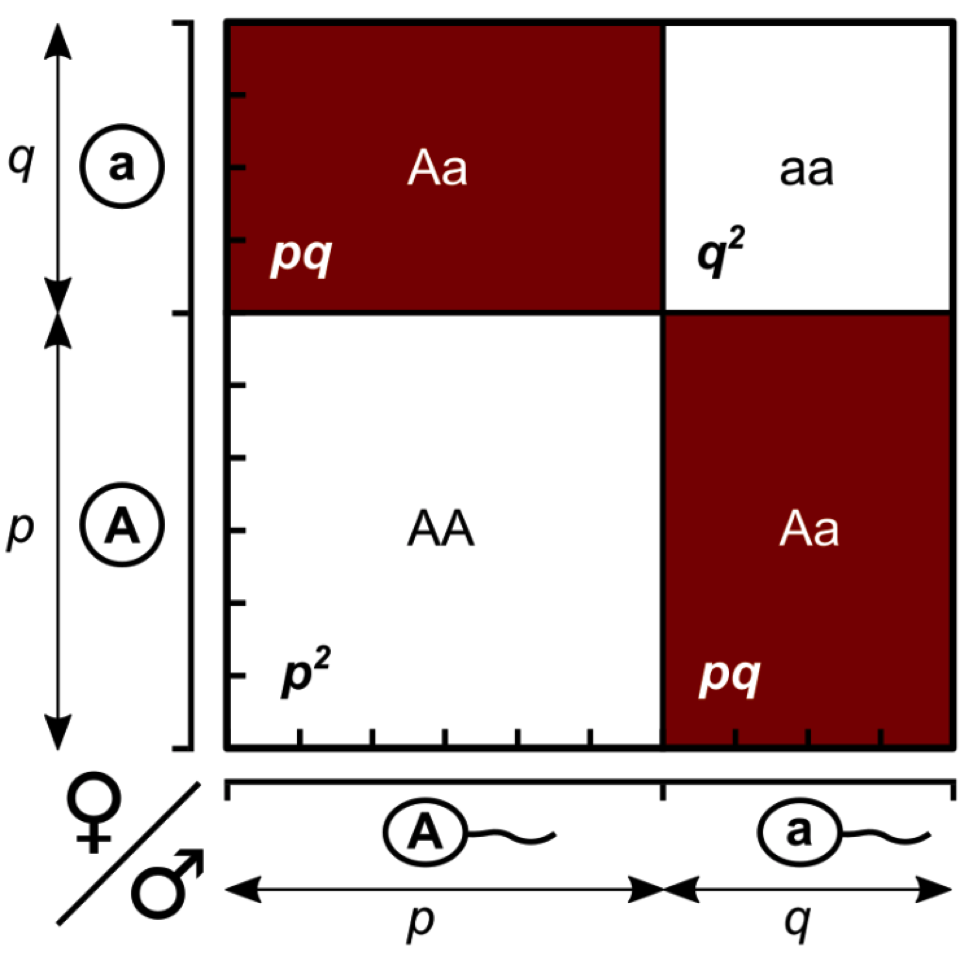
\includegraphics[width=0.8\linewidth]{ApuntesGeneticaII_files/figure-latex/HWpunnett-1} 

}

\caption{Cuadrado de Punnett con frecuencias $p=0,6$ y $q=0,4$. Las áreas de los rectángulos/cuadrados representan las frecuencias de los genotipos. Figura tomada de Wikipedia (CC0), modificada a partir de @pmid26354973}\label{fig:HWpunnett}
\end{figure}

Una forma gráfica de ver estos resultados son los llamados ``cuadrados de
Punnett''\footnote{Reginald Crundall Punnett, genetista británico que fue quien los
  desarrolló. Además, Punnett se relaciona directamente con el
  equilibrio de Hardy-Weinberg, ya que al no poder contrarrestar los
  argumentos de George Udny Yule acerca del crecimiento sostenido de
  los alelos dominantes, llevó el problema al matemático Godfrey
  Harold Hardy, con quien jugaba al cricket; el resto es historia
  conocida.}, como el que se aprecia en la Figura \ref{fig:HWpunnett}.
En la misma, en el eje horizontal tenemos la frecuencia con la que
aparecen los gametos masculinos, mientras que en el vertical aparecen
las frecuencias de los gametos femeninos; por lo tanto, el producto de
estas frecuencias será el área de los rectángulos y cuadrados
correspondientes (de geometría elemental, el área de cuadrados y
rectángulos es el producto de dos lados contiguos). Se observa además
claramente el origen del factor 2 en los heterocigotos (la suma de las 2
áreas coloreadas en rojo, cada una con valor \(pq\)).

\begin{graybox}

Hardy-Weinberg en \textbf{un locus con dos alelos}, considerando una especie \textbf{hermafrodita diploide}

\begin{itemize}
\item
  En el equilibrio, las frecuencias de los genotipos \(A_1A_1\),
  \(A_1A_2\) y \(A_2A_2\) serán \(p^2\), \(2pq\) y \(q^2\), respectivamente.
\item
  Las frecuencias de los alelos (\(p\) y \(q\)) no cambian luego de una
  generación de apareamiento y por lo tanto, como este razonamiento se
  puede extender a la próxima generación también, no cambiará nunca
  (mientras no intervengan otras fuerzas evolutivas como la selección
  o la deriva y el apareamiento sea al azar).
\item
  Las frecuencias de los genotipos quedan completamente determinados
  por la frecuencia de los alelos en la generación previa (porque son
  las frecuencias de los gametos, haploides) y en el caso particular
  de nuestro modelo de un locus con dos alelos, todo queda determinado
  por la frecuencia de uno de los dos alelos (\(p\), por ejemplo).
\item
  Además, en el caso particular de nuestro modelo, población
  hermafrodita, el equilibrio definitivo de las frecuencias de los
  genotipos se alcanza en una sola generación de apareamientos.
\end{itemize}

\end{graybox}

\subsection*{Supuestos que asumimos se cumplen para H-W}\label{supuestos-que-asumimos-se-cumplen-para-h-w}
\addcontentsline{toc}{subsection}{Supuestos que asumimos se cumplen para H-W}

\begin{recuadro}

\begin{enumerate}
\def\labelenumi{\arabic{enumi}.}
\item
  Todos los genotipos poseen el mismo ``\emph{fitness}''\footnote{Esta condición involucra a todos los aspectos que pudieran llevar a diferencias en el éxito reproductivo. Por ejemplo, implica que no existan diferencias ni en la viabilidad de los diferentes genotipos hasta llegar a su etapa reproductiva, ni en la fecundidad de los mismos.} (es decir, ningún genotipo posee una ventaja respecto al número de descendientes que deja).
\item
  La población debe estar formada por un número infinitamente grande de individuos.
\item
  El apareamiento al azar debe producirse en toda la población.
\item
  No debe existir migración que altere las frecuencias.
\item
  Debe existir un equilibrio mutacional (es decir, las frecuencias de los alelos no varían pese a existir mutaciones).
\end{enumerate}

\end{recuadro}

\section{Hardy-Weinberg en especies dioicas (dos sexos)}\label{hardy-weinberg-en-especies-dioicas-dos-sexos}

Nuestro modelo previo fue extremadamente sencillo, pero su aplicación se ve
reducida a aquellas especies que son hermafroditas. Veamos entonces qué
ocurre en especies dioicas (\emph{i.e.}, con dos sexos separados). Supongamos, para mayor
generalidad que las frecuencias iniciales en los dos sexos son
diferentes, por lo que en la generación inicial tenemos \(p_{M}\) y
\(p_{H}\) (y por lo tanto \(q_{M}=1-p_{M}\) y
\(q_{H}=1-p_{H}\)). Ahora, los diferentes genotipos serán el
producto de combinar estos estos alelos con diferentes frecuencias en
machos y hembras:

\begin{equation}
\begin{split}
P(A_1A_1)=P(A_{1M})\cdot P(A_{1H})=p_{M}\cdot p_{H}\\
P(A_1A_2)=P(A_{1M})\cdot P(A_{2H})+P(A_{2M})\cdot P(A_{1H})=\\=p_{M}\cdot q_{H}+q_{M}\cdot p_{H}\\
P(A_2A_2)=P(A_{2M})\cdot P(A_{2H})=q_{M}\cdot q_{H}\\
\end{split}
\label{eq:eqHWdioicas}
\end{equation}

Como de estos apareamientos no esperamos diferencias en el número de
machos y hembras en cada una de las clases, a partir de ahora tanto
machos como hembras tendrán la misma frecuencia de los alelos \(A_1\) y
\(A_2\). ¿Pero cuál es esa frecuencia? Para encontrarla, simplemente
volveremos a sumar los alelos que aporta cada una de las clases,
ponderados por su frecuencia. Es decir, para el alelo \(A_1\), tendremos
que la nueva frecuencia \(p'\) se puede obtener sumando las contribuciones
de \(P(A_1A_1)\) y \(P(A_1A_2)\):

\begin{equation}
\begin{split}
p'=P(A_1A_1)+\frac{1}{2} P(A_1A_2)=p_{M}\cdot p_{H}+\frac{1}{2}(p_{M}\cdot q_{H}+q_{M}\cdot p_{H})
\end{split}
\label{eq:eqHWdioicas2}
\end{equation}

Multiplicando por 2 ambos lados de la ecuación y separando términos
obtenemos:

\begin{equation}
\begin{split}
2p'=2p_{M}\cdot p_{H}+p_{M}\cdot q_{H}+q_{M}\cdot p_{H} \\
2p'=p_{M}\cdot p_{H}+p_{M}\cdot p_{H}+p_{M}\cdot q_{H}+q_{M}\cdot p_{H}
\end{split}
\label{eq:eqHWdioicas3}
\end{equation}

Reordenando y sacando factor común, tenemos:

\begin{equation}
\begin{split}
2p'=(p_{M}\cdot p_{H}+p_{M}\cdot q_{H})+(p_{M}\cdot p_{H}+q_{M}\cdot p_{H})\\
2p'=p_{M} (p_{H}+q_{H}) + p_{H} (p_{M}+q_{M})= p_{M} (1) + p_{H} (1) \\
2p'= p_{M}+ p_{H} \Leftrightarrow p'=\frac{p_{M}+ p_{H}}{2} 
\end{split}
\end{equation}

\begin{equationbox}
\begin{equation}
p'=\frac{p_{M}+ p_{H}}{2}
\label{eq:eqHWdioicas4}
\end{equation}

\end{equationbox}

Es decir, \textbf{luego de la primer generación de apareamiento entre machos y hembras con diferentes frecuencias de los alelos \(A_1\) y\(A_2\), la frecuencia de ambos alelos será igual en machos y en hembras y su valor será \(p'=\frac{p_{M}+ p_{H}}{2}\) para el alelo \(A_1\) y \(q'=\frac{q_{M}+ q_{H}}{2}\) para el alelo \(A_2\)}. A este último resultado se puede llegar razonando por simetría (¿hubiera cambiado llamar al revés a los alelos?) o haciendo las cuentas:

\begin{equation}
\begin{split}
p'=\frac{p_{M}+ p_{H}}{2}=\frac{(1-q_{M})+(1-q_{H})}{2}=\\
=\frac{2-q_{M}-q_{H}}{2}=1-\frac{(q_{M}+q_{H})}{2} \therefore\\
\frac{(q_{M}+q_{H})}{2}=1-p'=q'
\end{split}
\label{eq:eqHWdioicas5}
\end{equation}

El último resultado está justificado, además, porque la suma de los alelos siempre debe
dar una frecuencia relativa de 1. Más allá de todas las cuentas que nos
han llevado a estos resultados en forma analítica, una alternativa
primera sería utilizar el argumento de que el aporte de material
genético para formar la siguiente generación debe ser igual en machos
que en hembras: es decir, cada sexo aporta la mitad del material
genético (autosómico) de la nueva generación. Por lo tanto, la
frecuencia de los alelos en la generación de hijos debe ser el promedio
de las frecuencias en sus padres, que es el resultado que hemos visto.

\subsubsection*{Ejemplo 2.1}\label{ejemplo-2.1}
\addcontentsline{toc}{subsubsection}{Ejemplo 2.1}

El genotipado molecular (``\emph{chips}'') nos permite conocer
las bases (A, C, G, T) particulares que presenta un animal en diferentes
posiciones del genoma, desde unas pocas posiciones a centenas de miles
(\emph{e.g.}, alrededor de 700 mil, en algunos ``\emph{chips}''). Estos
marcadores se conocen como SNPs (``\emph{Single Nucleotide Polymorphisms}'', en inglés) y si
bien son relativamente poco informativos como marcadores (se suelen
escoger marcadores bi-alélicos en el diseño), su elevado número los
transforma en una herramienta sumamente poderosa. Usando un ``\emph{chip}''
comercial para bovinos en 1000 animales no emparentados de la raza
``Guernsey'' se encontró que el SNP \textbf{rs43375517}, en la región 5'UTR del
gen ARL4A y asociado a la producción de leche a 305 días en varios
estudios, presentaba las siguientes frecuencias de genotipos: CC 372, CG
476, GG 152. Calcular la frecuencia relativa de ambos alelos, así como
la esperanza del número observado de cada genotipo si la población se
encontrase en equilibrio de Hardy-Weinberg para este marcador.

\begin{figure}[H]

{\centering 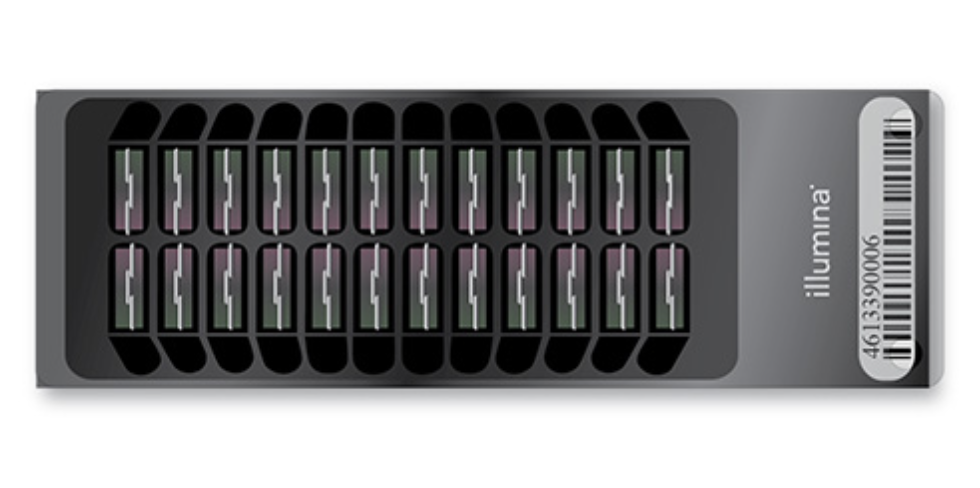
\includegraphics[width=0.8\linewidth]{figuras/IlluminaBovineSNP50v3} 

}

\caption{Chip "BovineSNP50 v3" de genotipado Bovino, de la empresa Illumina, con capacidad para analizar simultaneamente en 24 muestras 53218 SNPs altamente informativos (fotografía e información de la página de Illumina).}\label{fig:IlluminaBovineSNP50v3}
\end{figure}

Dado que tenemos 1000 individuos genotipados (372+476+152=1000), el
número total de alelos en genotipados es 2000 (son individuos
diploides). La frecuencia relativa del alelo `C', llamémosle \(p\), es:

\begin{equation}
p=\frac{2\times 372+1\times 476}{2000}=\frac{744+476}{2000}=\frac{1220}{2000}=0,61,
\end{equation}

por lo que, la frecuencia relativa del alelo `G' es \(q=1-p=0,39\). Si la
población se encontrase en equilibrio de Hardy-Weinberg, con 1000
individuos genotipados esperaríamos obtener las siguientes frecuencias:

\begin{equation}
\begin{split}
CC=p^2\times 1000=0,61^2\times 1000=0,3721\times 1000=372,1\\
CG=2pq\times 1000=2\times 0,61\times 0,39=0,4758\times 1000=475,8\\
GG=q^2\times 1000=0,39^2\times 1000=0,1521\times 1000=152,1,
\end{split}
\end{equation}

lo que más allá de las diferencias atribuibles al redondeo (es imposible genotipar
fracciones de individuo, pero incrementando el tamaño de la muestra
estos errores pueden reducirse más), tenemos un ajuste casi perfecto a
las expectativas del equilibrio Hardy-Weinberg.

\section{H-W: la frecuencia de heterocigotas en función de la frecuencia alélica}\label{heterocigotas-freq-alelica}

En un locus con dos alelos, ¿a qué frecuencia del alelo \(p\) podemos
observar la mayor frecuencia de heterocigotas, asumiendo que la
población se encuentra en equilibrio de Hardy-Weinberg?
La alternativa más sencilla para tener una idea aproximada del
comportamiento del número de heterocigotas bajo estos supuestos es
graficar la misma como función de \(p\). Tenemos que \(2pq=2p(1-p)\), y podemos graficar esta relación en cualquier
software que permita graficar funciones, calculadora, o aún en una
planilla electrónica (por ejemplo generando una serie en el intervalo
0-1). La Figura \ref{fig:HWheterop} es el resultado de graficar esta función, donde
se ve que la máxima frecuencia de heterocigotas se encuentra en el
entorno de \(p=0,5\), o sea en frecuencias intermedias de los dos alelos; la máxima proporción de heterocigotas esperable para una población
en equilibrio de HW es \(0,5\).

\begin{figure}[H]

{\centering 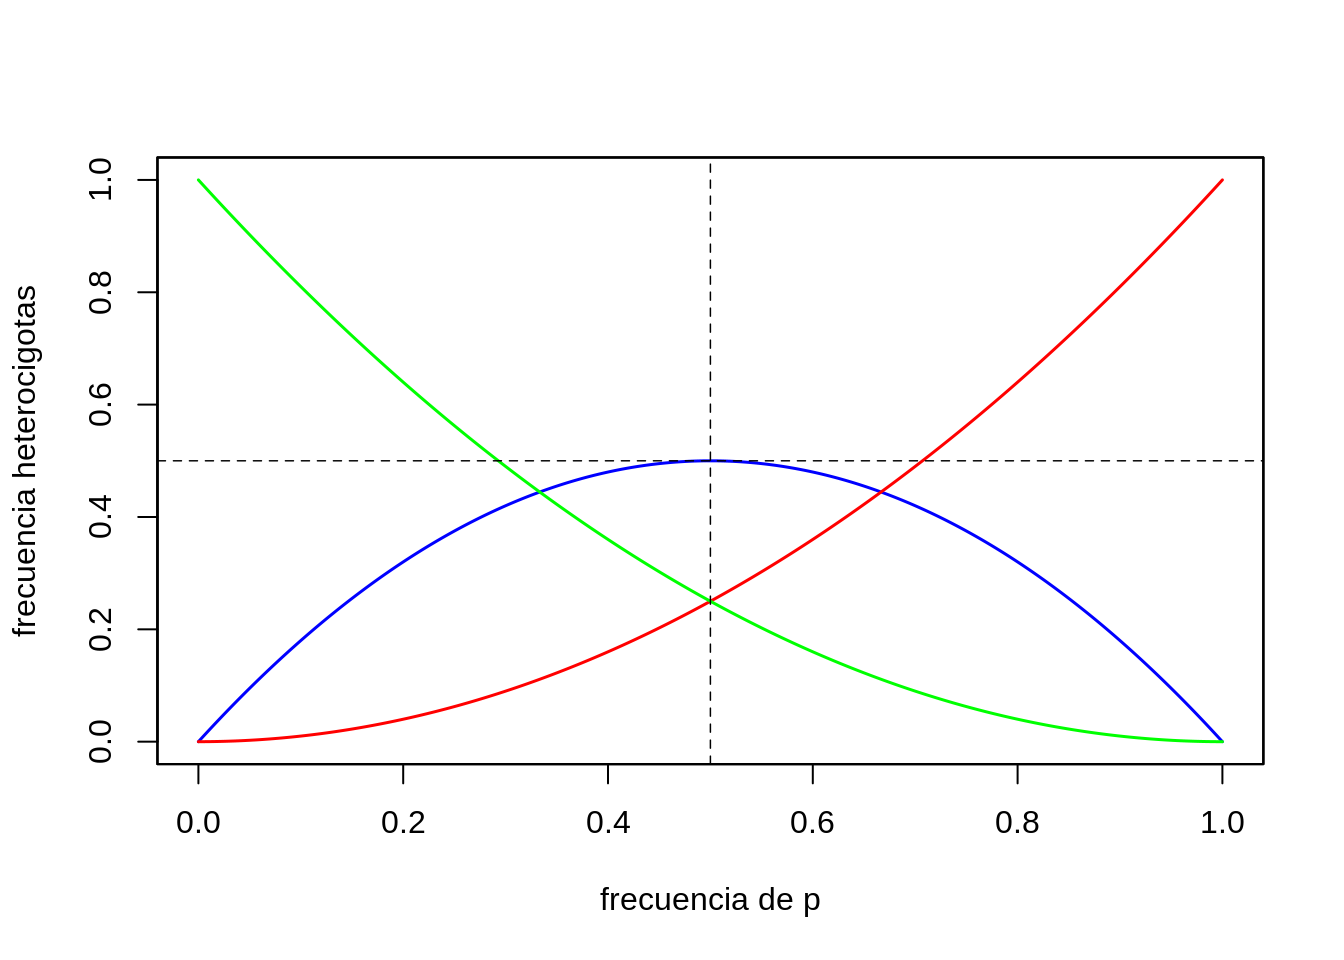
\includegraphics[width=0.8\linewidth]{ApuntesGeneticaII_files/figure-latex/HWheterop-1} 

}

\caption{Frecuencia de heterocigotas en función de la frecuencia del alelo $p$ en un modelo de un locus con dos alelos, bajo equilibrio Hardy-Weinberg. En azul la frecuencia de los heterocigotas, rojo y verde los homocigotas.}\label{fig:HWheterop}
\end{figure}

Una forma más precisa, complementaria con la anterior, es el estudio
analítico de esta función. Es decir, dada la función
\(f_{Het}(p)=2pq=2p(1-p)=2p-2p^2\), podemos reconocer los extremos relativos
(máximos y mínimos) de la misma como los lugares donde la pendiente de
la recta tangente es igual a cero. Lo que es equivalente, estos son los puntos
donde la derivada primera de la función se hace cero. Por lo tanto, derivando la
función obtenemos:

\begin{equation}
\begin{split}
f_{Het}(p)=2pq=2p(1-p)=2p-2p^2\\
\frac{d f_{Het}}{dp}=2-4p\\
2-4p=0  \Leftrightarrow p=\frac{1}{2}
\end{split}
\end{equation}

Es decir, la función tiene un solo máximo o mínimo en \(p=\frac{1}{2}=0,5\). Para
reconocer de cuál de los dos se trata es necesario ver el signo de la
derivada segunda (lo que hacemos volviendo a derivar la derivada primera):

\begin{equation}
\frac{d^2 f_{Het}(p)}{dp^2}=-4
\end{equation}

Como el signo es negativo, se trata de un máximo. Más aún, la forma de función original
(\(f_{Het}=2p-2p^2\)) es claramente reconocible como la de una parábola
con forma de ``U'' invertida y cuyas intersecciones con el eje de las
abcsisas (raíces) son 0 y 1, por lo que por simetría el vértice debe
estar en el punto medio (es decir, \(\frac{1}{2}\)). Sustituyendo, tenemos:

\begin{equation}
\begin{split}
f_{Het_{max}}(p=\frac{1}{2})=2p-2p^2=2 \frac{1}{2}-2\left(\frac{1}{2}\right)^2=\\
2 \frac{1}{2} -2 \frac{1}{4} =1- \frac{1}{2}=\frac{1}{2}
\end{split}
\end{equation}

\section{El equilibrio de Hardy-Weinberg en cromosomas ligados al sexo}\label{el-equilibrio-de-hardy-weinberg-en-cromosomas-ligados-al-sexo}

En los razonamientos previos hemos asumido que el locus de interés era
autosómico, es decir que no estaba en uno de los cromosomas sexuales
¿Qué ocurriría si este locus se encuentra en el cromosoma X del sistema
\textbf{XY} de determinación del sexo?\footnote{En el sistema \textbf{XY}, presente en los mamíferos, el gen Y es el
  que determina el sexo (masculino), siendo los machos heterogaméticos
  (XY) y las hembras homogaméticas (XX). Es otras especies, como las
  aves, existen otros sistemas como el \textbf{ZW}, en el que son las
  hembras las que son heterogaméticas (ZW), mientras que los machos
  son homogaméticos (ZZ)}\\
A diferencia de antes, los machos poseen ahora solo un cromosoma X (son
hemicigotas), que es donde está nuestro locus de interés y que por lo
tanto tienen el alelo \(A_1\) con probabilidad \(p_{M}\) y el alelo
\(A_2\) con probabilidad \(q_{M}=1-p_{M}\). En las hembras tenemos
los dos cromosomas X y en ambos los alelos \(A_1\) y \(A_2\) tendrán
probabilidad \(p_{H}\) y \(q_{H}\)
respectivamente (con \(q_{H}=1-p_{H}\)). Las hembras descendientes de este cruzamiento tendrán
dos cromosomas X, uno del padre y otro de la madre, y las frecuencias de
los genotipos serán equivalentes a los de las ecuaciones
\eqref{eq:eqHWdioicas} y siguientes. En cambio, los machos tienen un
solo cromosoma X, aportado por la madre (el padre aporta el cromosoma Y), y por lo tanto las frecuencias de los alelos \(A_1\) y \(A_2\) en esta nueva generación de machos serán iguales a las frecuencias del respectivo
alelo en las hembras de la generación anterior.

En resumen, en la nueva generación de machos y hembras (la distinguimos
de la anterior con ') tendremos ahora las siguientes frecuencias:

\begin{equation}
\begin{split}
p'_{H}=\frac{p_{M}+ p_{H}}{2} \\
q'_{H}=\frac{q_{M}+ q_{H}}{2} \\
p'_{M}=p_{H} \\
q'_{M}=q_{H}
\end{split}
\end{equation}

El mismo razonamiento lo podemos extender para la próxima generación (la distinguimos de la anterior con ``), por lo que ahora tendremos:

\begin{equation}
\begin{split}
p''_{H}=\frac{p'_{M}+ p'_{H}}{2}=\frac{p_{H}+\frac{p_{M}+ p_{H}}{2}}{2}  \\
q''_{H}=\frac{q'_{M}+ q'_{H}}{2}=\frac{q_{H}+\frac{q_{M}+ q_{H}}{2}}{2} \\
p''_{M}=p'_{H}= \frac{p_{M}+ p_{H}}{2} \\
q''_{M}=q'_{H}=\frac{q_{M}+ q_{H}}{2}
\end{split}
\end{equation}

\begin{figure}[H]

{\centering 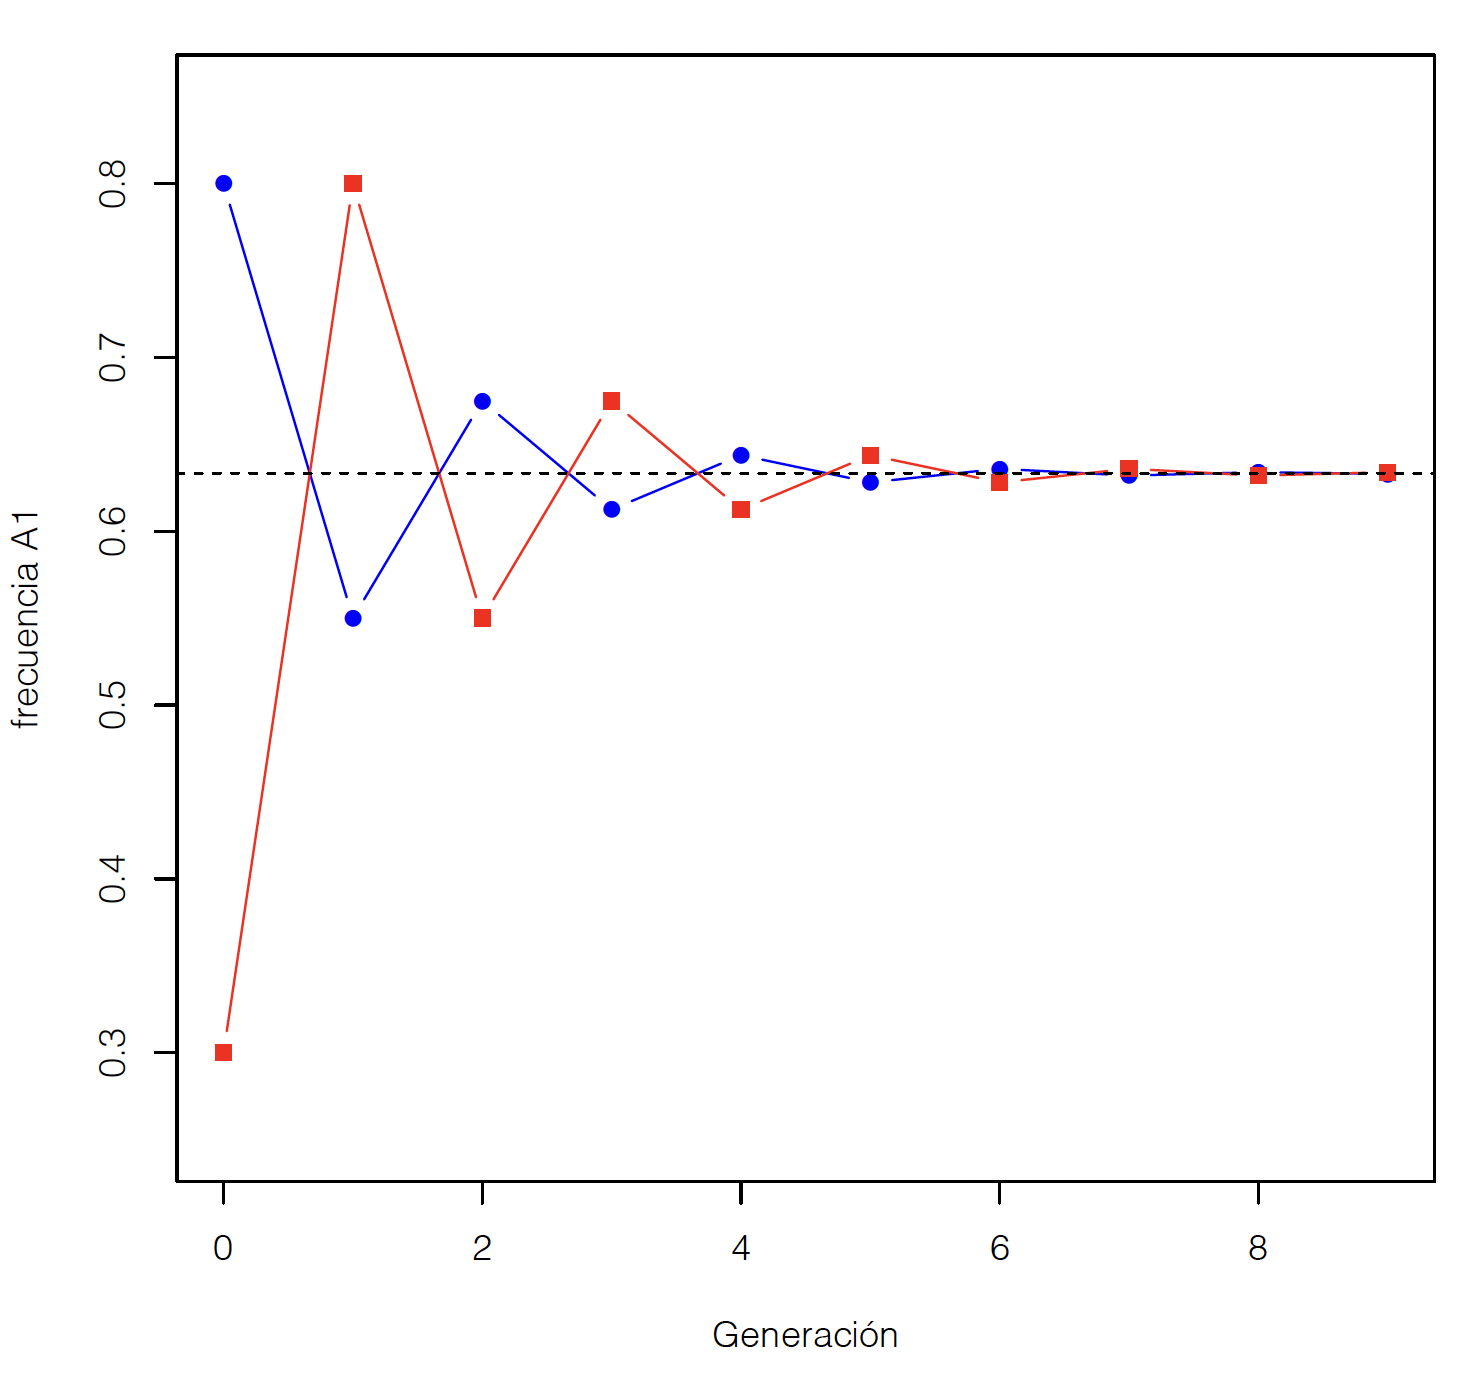
\includegraphics[width=0.8\linewidth]{figuras/HW_cromosomaX} 

}

\caption{Evolución de las frecuencias alélicas en machos (cuadrados rojos) y hembras (círculos azules) en un locus perteneciente al cromosoma X en especies en que el Y determina el sexo. La línea a trazos negros representa la media de la población. Las frecuencias de partida (generación 0) son $p_{M}=0,3$ y $p_{H}=0,8$.}\label{fig:HWcromosomaX}
\end{figure}

O sea, hemos establecido una regla de recurrencia para calcular las
frecuencias de \(p\) y \(q\) a partir de la generación anterior (se
puede llegar hasta la generación inicial), pero aún no hemos estudiado el
comportamiento a largo plazo de este proceso. Para entenderlo mejor
podemos resumir la información, como aparece en el siguiente cuadro, donde además de
las frecuencias del alelo \(A_1\) para hembras y machos en las 3 primeras
generaciones también calculamos la frecuencia del alelo en toda la
población (media) y la diferencia de frecuencias entre hembras y machos.

\begin{table}
\centering
\begin{tabular}[t]{rllll}
\toprule
$\textbf{Generación}$ & $A_{1H}$ & $A_{1M}$ & $\text{Media}$ & $\text{Diferencia}$\\
\midrule
\cellcolor{gray!10}{0} & \cellcolor{gray!10}{$p_{H}$} & \cellcolor{gray!10}{$p_{M}$} & \cellcolor{gray!10}{$\frac{2 p_{H}+p_{M}}{3}$} & \cellcolor{gray!10}{$p_{H}-p_{M}$}\\
1 & $\frac{p_{M}+ p_{H}}{2}$ & $p_{H}$ & $\frac{2 p_{H}+p_{M}}{3}$ & $\frac{p_{M}-p_{H}}{2}=-\frac{(p_{H}-p_{M})}{2}$\\
\cellcolor{gray!10}{2} & \cellcolor{gray!10}{$\frac{p_{H}+\frac{p_{M}+ p_{H}}{2}}{2}$} & \cellcolor{gray!10}{$\frac{p_{M}+ p_{H}}{2}$} & \cellcolor{gray!10}{$\frac{2 p_{H}+p_{M}}{3}$} & \cellcolor{gray!10}{$\frac{p_{H}-p_{M}}{4}$}\\
\bottomrule
\end{tabular}
\end{table}

Es de notar que para calcular la frecuencia del alelo en la población,
debemos ponderar la frecuencia en hembras por 2/3 y la de machos por
1/3, ya que esas son las proporciones de cromosomas X que aportan cada
uno de los sexos a la población.

Si nos fijamos en la columna de la media en el cuadro anterior, lo primero que
observamos es que la misma no cambia con el tiempo. Es decir, la
frecuencia general en la población de los alelos \(A_1\) y \(A_2\) está
determinada desde el principio, y su valor es

\begin{equationbox}
\begin{equation}
p=(2 p_{H}+p_{M})/3. 
\end{equation}

\end{equationbox}

Lo segundo que podemos apreciar, si
observamos la columna que muestra la diferencia entre los dos sexos, es
que el valor absoluto de esta diferencia se va reduciendo a la mitad en
cada generación, mientras que el signo de la misma alterna de generación
en generación. Con estas observaciones en mano es fácil entender que el proceso tiende
igualar las frecuencias entre los dos sexos (asumiendo que parten de
valores diferentes en machos y hembras). Si bien teóricamente estas frecuencias nunca llegan a ser iguales, desde el punto de vista práctico la diferencia es
despreciable luego de unas pocas generaciones, y en general los
procesos estocásticos (\emph{e.g.}, la deriva, que veremos más adelante)
tendrán un impacto mucho mayor que estas diferencias.\\
El comportamiento de estas frecuencias puede observarse gráficamente
también, como lo muestra por ejemplo la Figura
\ref{fig:HWcromosomaX},
partiendo en este caso de \(p_{M}=0,3\) y \(p_{H}=0,8\). Se
aprecia claramente en esta figura que \emph{a)} la frecuencia en machos es igual a
la frecuencia en las hembras de la generación anterior, \emph{b)} la
frecuencia en hembras es el promedio de las frecuencias de machos y
hembras en la generación anterior, \emph{c)} la media de la población
permanece estable (línea a trazos negros), y \emph{d)} la
diferencia entre machos y hembras se reduce a la mitad en cada
generación.

\begin{graybox}

Para el equilibrio de Hardy-Weinberg en cromosomas ligados al sexo, asumiendo que el macho es el sexo heterogamético (al revés si la hembra lo es), tenemos:

\begin{itemize}
\item
  La frecuencia del alelo \(\bf{A_1}\) en \textbf{machos} (\(p_M\)) de la generación \(t\) es igual a \(p_H\) en la generación \(t-1\).
\item
  La frecuencia del alelo \(\bf{A_1}\) en \textbf{hembras} (\(p_H\)) de la generación \(t\) es igual a \(\frac{p_H+p_M}{2}\) en la generación \(t-1\).
\item
  Este proceso converge relativamente rápido al valor \(p=\frac{(2p_H+p_M)}{3}\), que es la frecuencia inicial de alelos \(p\) en el \textbf{\emph{pool} de gametos}.
\end{itemize}

\end{graybox}

\section{Tres o más alelos}\label{tres-o-muxe1s-alelos}

Hasta ahora hemos manejado los diferentes problemas asumiendo que se
trataba de un locus con únicamente dos alelos, lo que en principio
permite simplificar algunas cuentas ya que la frecuencia de \(q\) queda
determinada por la frecuencia de \(p\) (\emph{i.e.}, \(q=1-p\)). Sin embargo,
la extensión a tres o más alelos es relativamente sencilla y no requiere
de cosas nuevas, por más que aprovecharemos la oportunidad para
presentar el resultado central del equilibrio de Hardy-Weinberg de una
forma diferente.

Si recordamos nuestro modelo de dos alelos, podíamos representar el
conjunto de los alelos en la población como la suma de \(p\) y \(q\), es
decir \((p+q)\). Cuando hacemos el apareamiento en condiciones de
panmixia, estamos cruzando este \((p+q)\) con otro similar (porque los
alelos salen de la misma población), o lo que es equivalente:

\begin{equation}
(p+q)(p+q)=(p+q)^2=p^2+2pq+q^2
\end{equation}

De lo anterior surge
claro que podemos representar las frecuencias genotípicas esperadas en
el equilibrio Hardy-Weinberg como el cuadrado del binomio formado por
las frecuencias alélicas en la generación previa (frecuencias
gaméticas). Con esto en mano, resulta tentador extender este resultado a
más de 2 alelos. Supongamos entonces que tenemos un locus con 3 alelos,
\(A_1\), \(A_2\) y \(A_3\), con frecuencias respectivas \(p\), \(q\) y \(r\).
Nuestro ``todo'' estará ahora conformado por la suma de \(p\), \(q\) y \(r\), es
decir \((p+q+r)\), y el cruzamiento resultará en:

\begin{equationbox}
\begin{equation}
(p+q+r)(p+q+r)=(p+q+r)^2=p^2+q^2+r^2+2pq+2pr+2qr
\end{equation}

\end{equationbox}

Es decir, si llamamos \(A_i\) a los \(i=1,2,...,k\) alelos diferentes, y \(p_i\) a
las frecuencias correspondientes, la frecuencia de los genotipos
homocigotas estará determinada por \(p_{i}p_{i}=p_{i}^2\) y la de los
heterocigotas por \(2p_{i}p_{j}, i \neq j\). Obviamente, el razonamiento
del binomio y del trinomio se puede extender a un número mayor de
alelos.

En general, para \(k\) alelos diferentes, el número de genotipos
heterocigotas es igual a \(k(k-1)/2\). Para ver de dónde se desprende
esto, es fácil imaginar un ``cuadrado de Punnett'', ahora con 3 o más
alelos. El total de celdas del cuadrado es \(k*k=k^2\), de las cuales, los
homocigotas serán las celdas que se encuentren en la diagonal, o sea \(k\)
celdas. Esto nos deja \(k^2-k=k(k-1)\). Sin embargo, las celdas simétricas
respecto a la diagonal representan el mismo genotipo (\emph{i.e.}, \(p_{ij} \equiv p_{ji}, \forall i \neq j\); de ahí el factor 2 para los
heterocigotas), por lo que al total de celdas que nos quedaban debemos
dividirlo entre 2 para tener el número de genotipos heterocigotos y de
ahí que este sea igual a \(k(k-1)/2\). Finalmente, el número total de
genotipos es la suma de homocigotos (\(k\)) y heterocigotos (\(k(k-1)/2\)). Es
decir, el número de genotipos corresponde a \(k+k(k-1)/2=(2k/2)+k(k-1)/2=k(k+1)/2\).\\
De acuerdo a lo anterior, la frecuencia total de homocigotos será:

\begin{equationbox}
\begin{equation}
G=\sum_{i=1}^{k} p_{i}^2,
\end{equation}

\end{equationbox}

lo que nos deja la posibilidad
de definir la heterocigosis del locus como lo que falta para completar
la totalidad, o sea:

\begin{equationbox}
\begin{equation}
H=1-G=1-\sum_{i=1}^{k} p_{i}^2
\end{equation}

\end{equationbox}

Es importante entender que
la fórmula anterior no es función de la proporción real de heterocigotos
que existen en una población determinada para un locus dado, sino que se
trata de la esperanza en función de las frecuencias alélicas, si se
cumpliera el equilibrio de Hardy-Weinberg.

\begin{graybox}

\begin{itemize}
\tightlist
\item
  Para 3 alelos el equilibrio de Hardy-Weinberg es la expansión del cuadrado del trinomio, es decir para los alelos \(\bf{A_1}\), \(\bf{A_2}\), \(\bf{A_3}\), con frecuencias respectivas \(p\), \(q\) y \(r\), \(p+q+r=1\),
\end{itemize}

\begin{equation}
(p+q+r)^2=p^2+q^2+r^2+2pq+2pr+2qr
\end{equation}

los 3 primeros términos de la derecha correspondientes a los homocigotos \(\bf{A_1A_1}\), \(\bf{A_2A_2}\), \(\bf{A_3A_3}\) y el resto a los heterocigotos \(\bf{A_1A_2}\), \(\bf{A_1A_3}\) y \(\bf{A_2A_3}\).

\begin{itemize}
\tightlist
\item
  La ecuación anterior es generalizable a un número \(k\) de alelos, \(\bf{A_1}, \bf{A_2}, ..., \bf{A_k}\) de acuerdo a
\end{itemize}

\begin{equation}
(p_1+p_2+p_3...+p_k)^2
\end{equation}

\begin{itemize}
\tightlist
\item
  Bajo equilibrio de Hardy-Weinberg, la proporción esperada de \textbf{homocigotas} será
\end{itemize}

\begin{equation}
G=\sum_{i=1}^{k} p_{i}^2,
\end{equation}

por lo que la heterocigosis del \emph{locus} quedará como lo que falta para completar
la totalidad, o sea:

\begin{equation}
H=1-G=1-\sum_{i=1}^{k} p_{i}^2
\end{equation}

\end{graybox}

\section{La estimación de frecuencias y el equilibrio (o no)}\label{la-estimaciuxf3n-de-frecuencias-y-el-equilibrio-o-no}

En una población con un gran número de individuos, tendiendo a
infinito, si la población se encuentra en equilibrio de Hardy-Weinberg
el número de individuos de los distintos genotipos coincidirá
estrechamente con las esperanzas de los mismos a partir las frecuencias
de los alelos. Es decir, la variación estocástica en cada uno de los
apareamientos (o en la unión de los gametos) tiende a cancelarse cuando
consideramos el gran número de individuos en la población. Sin embargo,
aún en esas grandes poblaciones no solemos tener acceso a la información
de todos los individuos y sí, solamente, a la información de una
\textbf{muestra aleatoria} de la misma. El concepto de muestra aleatoria es
fundamental ya que será el que nos permitirá extender nuestras
conclusiones de la muestra hacia la población, que en última instancia
suele ser lo que nos interesa. Al trabajar con una muestra aleatoria
relativamente reducida de la población, los números ahora serán mucho
menores, y por lo tanto los efectos del azar se verán incrementados.\\
Supongamos, para ver el impacto del tamaño de la muestra, que tenemos
interés en estimar las frecuencias de los dos alelos en un locus
autosomal de una especie diploide en una población determinada. Como se
trata de una especie salvaje, difícil de capturar para muestrear, nos
contentamos con los 5 individuos que pudimos genotipar para este locus;
sin duda es mucho mejor que no tener nada. Como se trata de una especie
diploide, si tenemos \(n\) individuos vamos a tener \(2n\) alelos
genotipados (\emph{i.e.}, 10 alelos genotipados). Supongamos ahora que de esos 10 alelos genotipados, 3
fueron del alelo \(A_1\) y 7 del alelo \(A_2\). Es decir, la proporción de
\(A_1\) es igual a \(p=3/10=0,3\), mientras que la del alelo \(A_2\) es de
\(q=7/10=0,7\) (hubiésemos llegado también a este resultado como \(q=1-p\)).
Parece razonable usar este valor de \(p\) como un \textbf{estimador} del
``verdadero valor''\footnote{Ya veremos en otras partes que el concepto de ``verdadero valor'' de
  un parámetro está ligado a una corriente estadística llamada
  ``frecuentista'' y que se contrapone en cierta manera a una visión más
  subjetiva de la probabilidad, representada en la escuela
  ``bayesiana''.} del parámetro en la población, en este caso la
frecuencia del alelo \(A_1\), tanto que coincide con el estimador por
máxima verosimilitud (es decir, escogemos como valor estimado aquel que tiene mayor probabilidad de ocurrir de acuerdo a lo que hemos observado).

Ahora, ¿que certeza tenemos que este valor que estimamos esté cerca del
``verdadero valor''? En principio, como solo tenemos 10 alelos
genotipados, nuestras estimaciones irán de 10\% en 10\% (los saltos en la
cuenta de alelos son de a 1, pero en 10 total, así que tenemos
\(\frac{1}{10}=0,1=10\%\)). O sea, la precisión de nuestra estimación es
realmente baja.

Otra forma de ver este problema es pensar en cuál sería la probabilidad
de observar este conteo de alelos \(A_1\), por ejemplo, dado que conocemos
el verdadero valor del parámetro. Si suponemos que los individuos
representan un muestreo al azar de los gametos en la población y que los
individuos de la muestra fueron seleccionados al azar, entonces la
probabilidad de observar un conteo \(x\) en particular, dado el número
total de alelos genotipados \(n\), se puede describir por la distribución
binomial (en nuestro caso de dos alelos):

\begin{equation}
\begin{split}
f(x)={n\choose x} p^x (1-p)^{n-x}
\end{split}
\label{eq:binomi}
\end{equation}

con las combinaciones
de \(n\) elementos tomados de a \(x\) elementos iguales a:

\begin{equation}
\begin{split}
{n\choose x}=\frac{n!}{x!(n-x)!}
\end{split}
\end{equation}

Por ejemplo, si la frecuencia ``real'' en la población entera para el alelo \(A_1\) es de
\(p=0,5\), ¿cuál sería la probabilidad de observar este conteo en 3
alelos de los 10 que genotipamos? De acuerdo a la ecuación
\eqref{eq:binomi}, la
probabilidad de obtener 3 conteos en una muestra de 10, con una
probabilidad \(p=0,5\) en la población, es de:
\begin{equation}
f(3)={10\choose 3} (0,5)^3 (1-0,5)^{10-3}=\frac{10!}{7! 3!} (0,5)^3 (0,5)^{7}=\frac{10*9*8}{6} (0,5)^{10}=0,1171875 \sim 11,7\%.
\end{equation}
Es decir, aún cuando la frecuencia real en la población es de \(p=0,5\),
en más de 1 de cada 10 muestras que tomemos, solo por azar, observaremos
un conteo de 3 alelos. En estos casos, estimaríamos erróneamente \(p \approx 0,33\). Esto puede parecer poco, pero si nos fijamos en
la Figura \ref{fig:HWmuestrapeque2}(a), donde graficamos la probabilidad de
observar cada uno de los 11 conteos posibles (de 0 a 10 alelos \(A_1\)),
resulta claro que la probabilidad de no acertar en el único número
correcto (5 alelos), es realmente alta.

\begin{figure}[H]

{\centering 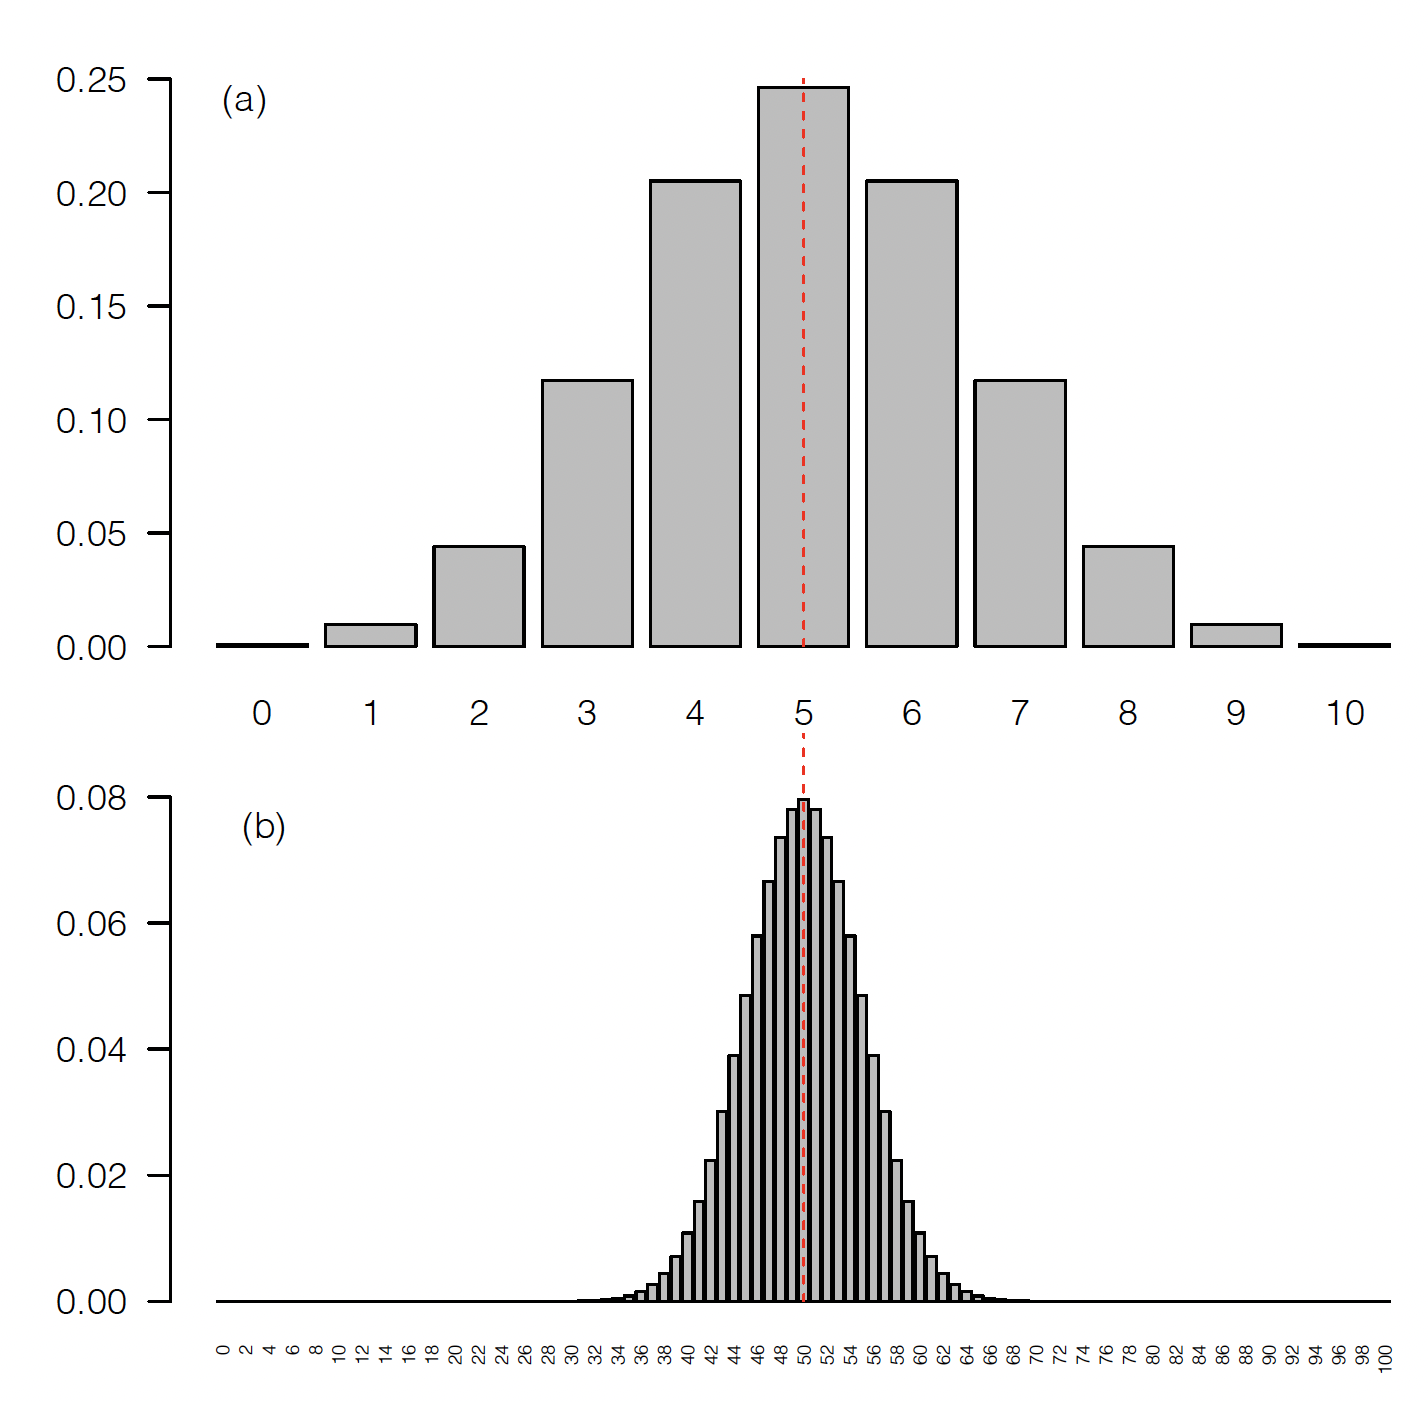
\includegraphics[width=0.8\linewidth]{figuras/HW_muestrapeque2} 

}

\caption{Probabilidad de observar un conteo de alelos determinado en una muestra de 5 individuos (a) y en una muestra de 50 individuos (b), dado que la frecuencia del mismo en la población es de 0,5.}\label{fig:HWmuestrapeque2}
\end{figure}

De hecho, si calculamos la
probabilidad de observar exactamente 5 alelos en 10, dada la frecuencia
real de \(p=0,5\), esta probabilidad es igual a \(0,2460938\), por lo que la
probabilidad de \textbf{NO} obtener el ``verdadero'' valor de \(p\) en una muestra de
este tamaño es igual a \(1-0,2460938=0,7539062 \sim 75,4\%\). Por otro
lado, la probabilidad de tener un estimado de \(p \leq 0,3\) es la suma de
las probabilidades de obtener 0, 1, 2 o 3 conteos, y esto es igual a
\(0,171875 \sim 17,2\%\) (el lector lo puede verificar fácilmente).\\
Claramente, de lo anterior surge que este tamaño muestral de 5
individuos no nos conducirá a nada muy razonable. ¿Qué ocurriría si
conseguimos aumentar el tamaño muestral a 50 individuos? Las
probabilidades esperadas de los distintos conteos en la muestra
aleatoria se grafican en la Figura
\ref{fig:HWmuestrapeque2}(b). Ahora resulta claro que, por un lado,
la ``granularidad'' de las barras es mucho más fina (\emph{i.e.}, la
``precisión'' de nuestros estimados podría ser mucho mayor) y por el otro,
que las estimaciones muy alejadas del ``verdadero valor'' son bastante
improbables. Por ejemplo, ¿cuál sería la probabilidad de tener un
estimado de \(p \leq 0,3\)? En este caso se trata de la suma de las
probabilidades de todos los conteos, de 0 a 30 (\(30/100=0,3\)). En decir,
se trata de la \textbf{función de distribución} (a veces conocida como
probabilidad acumulada, o también CDF en inglés). En este caso, para la
distribución binomial, tenemos para un valor \(k\) (30 en nuestro caso)

\begin{equation}
\begin{split}
Pr(X \leq k)=\sum_{x=0}^{k} {n\choose x} p^x (1-p)^{n-x}
\end{split}
\label{eq:CDFbinom}
\end{equation}

Sería algo tedioso calcularlo a mano, pero una
primer idea del valor se puede tener observando la Figura
\ref{fig:HWmuestrapeque2}(b), donde resulta claro que las
probabilidades para conteos de hasta 30 son despreciables. De hecho,
utilizando la función de distribución en cualquier software que la tenga
implementada, la probabilidad de observar un conteo de 30 o menos alelos
en 100 genotipados es de 3,92507x10\textsuperscript{-5} (\(\sim 0,004\%\)) si la
frecuencia del alelo \(A_1\) en la población es \(p=0,5\); o sea,
prácticamente improbable.

Ahora también bajó la probabilidad de acertar \textbf{exactamente} en la estimación de \(p=0,5\).
¿Pero qué sucede con la probabilidad de obtener observaciones en un intervalo que nos lleve a una estimación razonablemente cercana a \(p = 0,5\)? Comparemos con nuestra muestra de 5 individuos, donde la probabilidad de observar exactamente 5
alelos era de \(\sim 24,6\%\). El interalo de frecuencias equivalente en nuestra muestra de 50 individuos corresponde al que contempla observar entre 45 y 54 alelos (probabilidades entre \(0,45\) y \(0,54\))\footnote{Si observamos \(45/100\) alelos en nuestro muestreo, nuestra estimación será \(p = 0,45\) (\(p = 0,5\), si redondeamos a una cifra significativa). Lo mismo sucedería si observamos cualquier valor entre 45 y 54 alelos.}; este intervalo concentra ahora \(\sim 63\%\) de la probabilidad. Dicho de otra manera, ahora los resultados se concentrarán (aproximadamente) entre 49 y 51 con una probabilidad similar a la que observabamos en nuestra muestra de 5 individuos. Claramente, nuestras estimaciones se vuelven mucho más precisas y útiles.

Hasta el momento hicimos nuestras estimaciones de las frecuencias alélicas
poblacionales (y, por lo tanto, la posibilidad de conocer nuestras
expectativas para el equilibrio de Hardy-Weinberg) de una manera
bastante sencilla: asumimos que -genómica mediante- podemos
acceder al verdadero estado alélico (\emph{e.g.}, ADN) de cada una de
las muestras. Sin embargo, en muchos casos esto no es posible.
Por ejemplo, puede desconocerse la base molecular de la diferencias fenotípicas observadas.
En otros casos, obtener esta información no es práctico, y la única información disponible es la fenotípica.
Por lo tanto, en estos casos solo contamos con el conteo de los distintos fenotipos.
Esto introduce un nuevo factor en el problema: es necesario conocer el
modelo de herencia (mendeliana,
{codominancia}, etc.) para poder pasar de los fenotipos
a los genotipos, y de allí a las frecuencias de los alelos.

Supongamos, para comenzar, que \textbf{el modelo de herencia es de {codominancia}} en un locus autosomal con dos alelos (\(A_1\)
y \(A_2\)) en una especie diploide. Bajo este modelo, ambos alelos se expresan en
el fenotipo y hay una correspondencia biunívoca entre fenotipo y
genotipo. En este caso tenemos tres genotipos que son
identificables directamente, por lo que podemos estimar las frecuencias relativas a partir del conteo de individuos.
PAra ello, tendremos en cuenta: \emph{a)} que los homocigotas presentan 2 alelos \(A_1\) y los heterocigotas 1, y
\emph{b)} que para \(n\) individuos tenemos \(2n\) alelos.
Así, en una muestra de \(n\) individuos la frecuencia relativa (muestral) del alelo \(A_1\) será igual
a la suma de 2 veces el número de homocigotas \(A_1\) más el número de
heterocigotas, todo dividido entre 2 veces el número de individuos:

\begin{equation}
\begin{split}
p=\frac{2n_{A_1A_1}+n_{A_1A_2}}{2n}, q=\frac{2n_{A_2A_2}+n_{A_1A_2}}{2n}\\
n=n_{A_1A_1}+n_{A_1A_2}+n_{A_2A_2}
\end{split}
\end{equation}

En todo caso, si conocemos los genotipos a nivel molecular (ver \hyperref[ejemplo-2.1]{Ejemplo 2.1}), la
forma de estimar es análoga al caso donde los genotipos corresponden en
forma biunívoca con los fenotipos\footnote{En estos casos observar el fenotipo aporta la misma información que determinar el genotipo}.
Tanto si se trata de un modelo de {codominancia} como de
dominancia parcial, lo relevante aquí es la posibilidad de
distinguir los heterocigotas de ambos homocigotas. Esto nos permite
simplemente hacer el ``conteo'' de alelos, ya que la base genética es
clara: en diploides, los homocigotas poseen dos alelos del mismo tipo y
los heterocigotas poseen uno de cada tipo.

Las cosas empiezan a complicarse un poco más cuando \textbf{aparece el efecto de dominancia}. Supongamos, por ejemplo, que en el locus anterior (autosomal en especie diploide, con dos alelos), el alelo \(A_1\) domina
completamente al \(A_2\). En este caso, tanto el genotipo \(A_1A_1\) como el \(A_1A_2\)
tendrán idéntico fenotipo, mientras que el \(A_2A_2\) tendrá un fenotipo
diferente. Estom implica que el conteo de fenotipos ya no permite
determinar las frecuencias de los ambos alelos, ya que los conteos del
fenotipo \(A_1\) corresponde al de dos genotipos en simultáneo (\(G_{11}=A_1A_1\) y
\(G_{12}=A_1A_2\)), ambos con diferente número de alelos \(A_1\) y \(A_2\)
(2 y 0 para el homocigota, 1 y 1 para el heterocigota). Dicho de otra
forma, sabemos calcular las frecuencias alélicas a partir de los 3
genotipos, pero solo contamos con dos fenotipos: el del alelo dominante y el
del alelo recesivo. De hecho, con solo esta información se trata de un
problema indeterminado. Para poder salir de esta situación debemos
agregar algún tipo de información adicional. Una alternativa sencilla
(suponiendo que no podemos conocer los genotipos, lo que resolvería
el problema) es \textbf{asumir que la población se encuentra en equilibrio de Hardy-Weinberg}. Esta asunción establece una relación explícita entre frecuencias alélicas (lo desconocido) y genotipos.
Notemos que el la clase genotípica \(A_2A_2\) (homocigota) es la única que corresponde con un único fenotipo.
Si la población se encuentra en equilibrio de Hardy-Weinberg, sabemos que la
esperanza del número de individuos para este genotipo es
igual a \(nq^2\), donde \(n\) es el número total de individuos (\(n=G_{1}.+G_{22}\)).
Sabemos además que el número de individuos con el fenotipo dominante está dado por \(G_{1}.=G_{11}+G_{12}\).
Esto nos permite estimar \(q\) (\emph{i.e.} la frecuencia del alelo \(A_2\)),

\begin{equation}
\begin{split}
G_{22}=nq^2 \therefore q=\pm \sqrt{\frac{G_{22}}{n}}=\pm \sqrt{\frac{G_{22}}{G_1.+G_{22}}}
\end{split}
\label{eq:HWrecesivos}
\end{equation}

De las dos raíces que tiene esta ecuación (una positiva y otra
negativa), solo una posee sentido biológico: no existen
frecuencias álelicas negativas, y por lo tanto dicha raíz no es una solución válida.
Es importante recalcar en este punto que la validez de nuestra
estimación depende de que la población se encuentre en equilibrio de
Hardy-Weinberg, pues de lo contrario no será una estimación que tenga
una base teórica.\\

\subsubsection*{Ejemplo 2.2}\label{ejemplo-2.2}
\addcontentsline{toc}{subsubsection}{Ejemplo 2.2}

La fenilcetonuria (PKU) es un error innato del
metabolismo que resulta en una disminución del metabolismo del
aminoácido fenilalanina. La enfermedad es resultado de una deficiencia en la enzima
fenilalanina hidroxilasa, codificada por el gen PAH. El resultado de esto es la acumulación de
fenilalanina a niveles potencialmente tóxicos. Desde el punto de vista
del modelo de herencia se comporta como autosómica recesiva, por lo que
es necesario heredar dos copias ``defectuosas'' del gen PAH (a decir
verdad, que tengan actividad seriamente disminuída) para que la
enfermedad se manifieste. La incidencia es muy variable de población en
población, pero dos casos extremos podrían ser el de la población de
Finlandia (1 afectado en 200 mil nacimientos) y el de la población de
Turquía (1 afectado en 2600 nacimientos). Calcular para ambas
poblaciones la frecuencia de ``el'' \footnote{Asumiremos que se trata de un solo tipo de alelo
  defectuoso. Si bien a nivel molecular los alelos defectuosos pueden
  ser de varios tipos diferentes, con efectos deletéreos, a nivel fenotípico se
  comportan como si se tratase de un mismo alelo (ver {[}Ejercicio 2.6{]}).} alelo defectuoso, así como la
proporción de portadores (que no manifiestan la enfermedad), asumiendo
que las poblaciones se encuentran en equilibrio de Hardy-Weinberg.\\
Utilizando la ecuación \eqref{eq:HWrecesivos}, tenemos para los dos casos

\begin{equation}
\begin{split}
q_{Fin}=\sqrt{\frac{1}{200000}}=0,002236068 \sim 0,22\% \\
q_{Tur}=\sqrt{\frac{1}{2600}}=0,01961161 \sim 1,96\%
\end{split}
\end{equation}

Los portadores serán los heterocigotas, por lo que, si asumimos que las
poblaciones se encuentran en equilibrio de Hardy-Weinberg, entonces
tendremos

\begin{equation}
\begin{split}
Het_{Fin}=2p_{Fin}q_{Fin}=2*(1-0,002236068)*0,002236068=0,004462136\sim 0,45\% \\
Het_{Tur}=2p_{Tur}q_{Tur}=2*(1-0,01961161)*0,01961161=0,038454 \sim 3,85\%
\end{split}
\end{equation}

\section{El sistema ABO}\label{el-sistema-abo}

Hasta el momento nos hemos centrado en el caso de un locus con dos alelos. En general, la relación entre los distintos alelos de un locus suele ser
más compleja. En principio, esto se debe a que existen más de dos alelos cuyo
impacto en el fenotipo es distinguible. A su vez, las relaciones entre dichos alelos puede ser variable, implicando muchas veces diferentes modos de herencia (\emph{e.g.}, dominancia y codominancia en el mismo locus). Un ejemplo de
esto es el sistema de grupos sanguíneos ABO, el más importante en
humanos,\footnote{Descubierto por el médico e inmunólogo austríaco Karl Landsteiner
  en 1901, lo que le valió el premio Nobel de Medicina y Fisiología en
  1931.} cuya herencia (en forma simplificada) puede apreciarse en
la Figura \ref{fig:ABOsystem}.

\begin{figure}[H]

{\centering 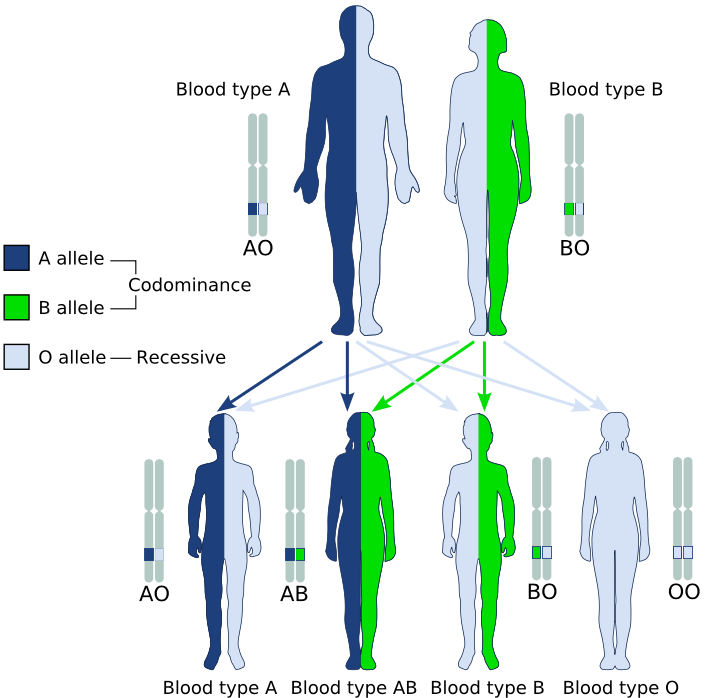
\includegraphics[width=0.7\linewidth]{figuras/ABOsystem} 

}

\caption{Sistema de determinación sanguínea ABO. Los alelos A y B muestran codominancia entre sí, mientras que ambos son dominantes respecto al O. Figura de Dominio Público tomada de Wikipedia ("ABO system codominance.svg").}\label{fig:ABOsystem}
\end{figure}

El locus codifica para antígenos de superficie en los eritrocitos (glóbulos rojos de
la sangre), existiendo tres alelos para el mismo. Básicamente, tanto el alelo \emph{\(I^A\)} como el \emph{\(I^B\)} (codificantes para los antígenos \textbf{A} y \textbf{B}, respectivamente) dominan al alelo \emph{\(i\)}, que
no produce antígenos de superficie (\textbf{O}). La relación entre el \emph{\(I^A\)}
y el \emph{\(I^B\)} es de codominancia, expresándose ambos antígenos en la superficie de los eritrocitos si estos alelos se encuentran presentes al mismo tiempo.
En función de las combinaciones alélicas posibles, existirán cuatro fenotipos diferentes detectables por los tests inmunológicos de rutina (\emph{i.e.}, test de aglutinación).

\begin{recuadro}

Si denominamos a las frecuencias de los alelos \emph{\(I^A\)}, \emph{\(I^B\)} e \emph{\(i\)} como \(p\), \(q\) y \(r\), respectivamente, estos cuatro fenotipos son definidos como

\begin{itemize}
\item
  Fenotipo \textbf{A}, formado por los homocigotas del alelo \emph{\(I^A\)} , más los
  heterocigotos del alelo \emph{\(I^A\)} y el alelo \emph{\(i\)}. La frecuencia esperada bajo equilibrio de Hardy-Weinberg es de \(p^2+2pr\).
\item
  Fenotipo \textbf{B}, formado por los homocigotas del alelo \emph{\(I^B\)} , más los
  heterocigotos del alelo \emph{\(I^B\)} y el alelo \emph{\(i\)}. La frecuencia esperada bajo equilibrio de Hardy-Weinberg es de \(q^2+2qr\).
\item
  Fenotipo \textbf{AB}, formado por los heterocigotas del alelo \emph{\(I^A\)} y el alelo
  \emph{\(I^B\)}. La frecuencia esperada bajo equilibrio de Hardy-Weinberg es de \(2pq\).
\item
  Fenotipo \textbf{O}, formado por los homocigotas del alelo \emph{\(i\)}. La frecuencia esperada bajo equilibrio de Hardy-Weinberg es de \(r^2\).
\end{itemize}

\end{recuadro}

Notemos que la estimación de las tres frecuencias a partir del conteo de individuos ya no
es tan sencilla como en los sistemas previamente analizados. Por un lado, existen en el sistema ABO 3 alelos en lugar de
dos. Por el otro, lo que realmente complejiza el panorama es la relación de dominancia-codominancia entre alelos.
De hecho, en casi todos los casos resulta imposible inferir el genotipo de un inviduo observando su fenotipo; en efecto, esto es solo posible para el fenotipo O (homocigotas del alelo \(i\)). En la Sección \hyperref[estimacion-abo]{La estimación de frecuencias en el locus ABO} se desarrolla un método para inferir las frecuencias alélicas a partir del conteo de los cuatro fenotipos detectables por el test de aglutinación.

\section{¿Dónde se ``esconden'' los alelos recesivos?}\label{duxf3nde-se-esconden-los-alelos-recesivos}

Muchas mutaciones tienen consecuencias deletéreas o muy graves cuando
están presentes en homocigosis, pero no tienen mayores consecuencias
para el individuo heterocigota. A modo de ejemplo, se puede pensar en un sistema que requiera de
una única copia funcional de una enzima para mantener una actividad metabólica necesaria. Resulta claro que una mutación en homocigosis puede afectar la actividad enzimática (\emph{e.g.}, alterando la capacidad de unión a ligando), alterando así a este sistema metabólico. No obstante, la misma mutación en heterocigosis no afectará la eficiencia del sistema, en tanto seguirá existiendo una copia funcional codificante para la enzima en cuestión.

La diferencia entre el efecto fenotípico de algunos alelos en homocigosis respecto a heterocigosis puede apreciarse también en casos donde una característica evolutivamente favorable se ha transformado con el paso del tiempo en algo negativo (\emph{e.g.}, debido a las
implicancias para la domesticación). Este es el caso de los cuernos en el
bovino. En las razas bovinas ``británicas'', la ausencia de
cuernos (mochos, o ``\emph{polled}'' en inglés) se trata de una característica que muestra un
evidente modo de herencia dominante. Aún habiéndose podido ``mapear'' la
ubicación de la característica en el genoma bovino, resulta bastante
elusivo el mecanismo que genera esta ausencia (Allais-Bonnet et al. (\citeproc{ref-pmid23717440}{2013});
Medugorac et al. (\citeproc{ref-pmid22737241}{2012})). Pese a esto, dado que los individuos con ambos alelos
astados (recesivos) presentan un fenotipo astado, resulta bastante tentador evitar que se
reproduzcan: intuitivamente se puede presumir que esto permitiría avanzar rápidamente en la eliminación de este alelo de la población, erradicandose así la existencia del fenotipo astado. Sin embargo, si se sigue esta premisa se observa un fenómeno interesante. Luego de una rápida caída en la proporción de individuos astados, el ritmo de la erradicación comienza a detenerse.
Nuestra percepción inicial era apenas una ilusión, y la erradicación del fenotipo comienza a parecer una meta cada vez más lejana. ¿Por qué sucede esto? El principal
problema con esta idea es que, al tratarse de un alelo recesivo el que
queremos eliminar, resulta imposible distinguir fenotípicamente a los individuos heterocigotas de los homocigotas para el alelo dominante. Para entenderlo, veamos qué ocurre
con la relación entre los heterocigotas y los homocigotas cuando nos acercamos a la eliminación del alelo. Sin pérdida de generalidad, llamaremos \(A_1\) al alelo dominante y \(A_2\) al alelo recisivo (con
frecuencias \(p\) y \(q\), respectivamente). En la situación planteada, tenemos que \(q \rightarrow 0\), y por lo tanto \(p \rightarrow 1\), por lo que la proporción de heterocigotas respecto a homocigotas estará dada por

\begin{equationbox}
\begin{equation}
\frac{2pq}{q^2}=\frac{2p}{q}=\frac{2(1-q)}{q}\approx \frac{2}{q} \therefore \lim_{q \to 0} \frac{2pq}{q^2}=+\infty
\end{equation}

\end{equationbox}

Es decir que, a medida que \(q\) tiende a cero, la relación tenderá a
infinito. Dicho de otra forma, la enorme mayoría de los alelos recesivos estarán
presentes en los individuos heterocigotas, los cuales son fenotípicamente indistinguibles de los homocigotas para el alelo dominante. La Figura
\ref{fig:HWheterohomoq} muestra gráficamente esta relación. A medida
que nos acercamos hacia la frecuencia de cero para el alelo \(A_2\) (\(q\)),
la pendiente de la relación se incrementa en valor absoluto (notemos que la derivada
primera es igual a \(-2/q^2\)) y rápidamente la función aparece como
vertical.

\begin{figure}[H]

{\centering 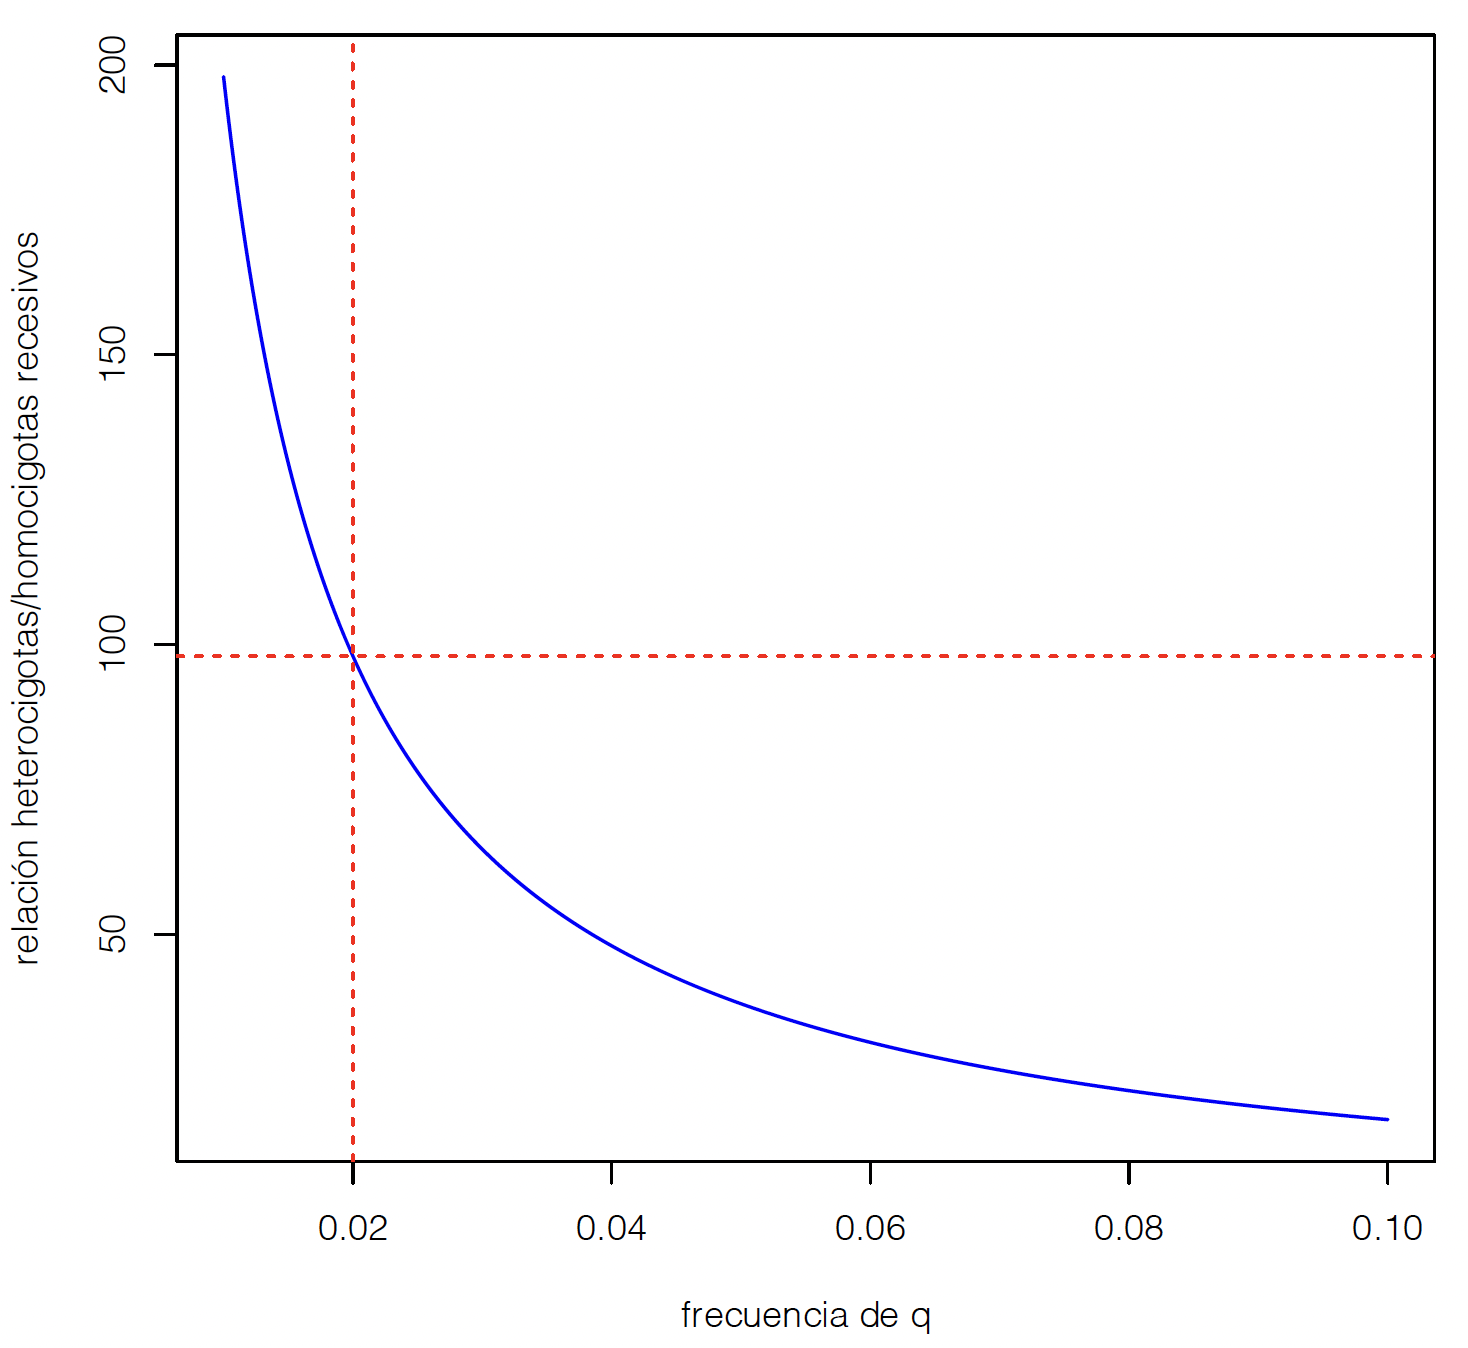
\includegraphics[width=0.75\linewidth]{figuras/HW_heterohomo_q} 

}

\caption{Relación del número de heterocigotas a homocigotas recesivos en función de la frecuencia del alelo $q$ en un modelo de un locus con dos alelos, bajo equilibrio Hardy-Weinberg.}\label{fig:HWheterohomoq}
\end{figure}

Como ya se había planteado, observamos que casi todos los alelos provienen de los
individuos heterocigotas. A una frecuencia \(q=0,02\) (\emph{i.e.}, el 2\% de los alelos
son \(A_2\)), hay 98 veces más individuos heterocigotas que homocigotas
recesivos. Pese a esto, si bien es imposible eliminar los alelos de la
población por este mecanismo, sí es posible reducir sustancialmente su
incidencia si mantener el criterio de ``refugo'' no tuviese otras
implicancias asociadas.

\subsubsection*{Ejemplo 2.3}\label{ejemplo-2.3}
\addcontentsline{toc}{subsubsection}{Ejemplo 2.3}

Con los datos del \hyperref[ejemplo-2.2]{Ejemplo 2.2},
calcular la relación entre el número de portadores y el número de
individuos que padecerán la enfermedad, asumiendo que las poblaciones se
encuentran en equilibrio de Hardy-Weinberg.

\begin{equation}
\begin{split}
q_{Fin}=\sqrt{\frac{1}{200000}}=0,002236068 \sim 0,22\% \\
q_{Tur}=\sqrt{\frac{1}{2600}}=0,01961161 \sim 1,96\%
\end{split}
\end{equation}

Los portadores serán los heterocigotas, por lo que, si asumimos que las
poblaciones se encuentran en equilibrio de Hardy-Weinberg, entonces
tendremos

\begin{equation}
\begin{split}
\frac{Het_{Fin}}{HomR_{Fin}}=\frac{2p_{Fin}}{q_{Fin}}=2*(1-0,002236068)/0,002236068=892,43 \\
\frac{Het_{Tur}}{HomR_{Tur}}=\frac{2p_{Tur}}{q_{Tur}}=2*(1-0,01961161)/0,01961161=99,98
\end{split}
\end{equation}

Es decir, en la población de Turquía tenemos casi 100 portadores por
cada enfermo, mientras que en la de Finlandia la relación es de
aproximadamente 892 portadores por cada enfermo.

\begin{graybox}

\begin{itemize}
\tightlist
\item
  La relación entre los heterocigotas y los homocigotas con el alelo
  recesivo (que sin pérdida de generalidad supondremos es el \(A_2\), con
  frecuencia \(q\)) cuando nos acercamos a la eliminación del alelo \(A_2\) y
  por lo tanto la frecuencia del \(A_1\) (\(p\)) se aproxima a 1 será:
\end{itemize}

\begin{equation}
\frac{2pq}{q^2}=\frac{2p}{q}=\frac{2(1-q)}{q}\approx \frac{2}{q} \therefore \lim_{q \to 0} \frac{2pq}{q^2}=+\infty
\end{equation}

\begin{itemize}
\tightlist
\item
  Es decir, a medida que \(q\) tiende a cero, la relación tenderá a
  infinito. Dicho de otra forma, \textbf{casi todos los alelos recesivos estarán
  en los individuos heterocigotas}, los que son fenotípicamente imposibles
  de distinguir de los homocigotas con el alelo dominante.
\end{itemize}

\end{graybox}

\section{Hardy-Weinberg en especies poliploides}\label{hardy-weinberg-en-especies-poliploides}

El fenómeno de la poliploidía (varias copias del genoma) representa un
importante factor evolutivo que lleva a la especiación y es bastante
usual en diferentes especies de todos los dominios de la vida, como se observa en la Figura \ref{fig:PaleopolyploidyTree}. En particular, la poliploidía es frecuente en muchas de las especies vegetales, y algunas animales, de interés productivo. Ejemplo de esto son las bananas
y sandías sin semillas (triploides), el maní y las moras (tetraploides),
o el trigo y el boniato (hexaploides). En algunos casos, como el de la frutilla,
el número básico de cromosomas (7) es repetido diferente número de
veces en las más de 20 especies, existiendo individuos diploides, tetraploides, hexaploides,
octaploides y hasta decaploides.

Las frecuencias alélicas esperadas en equilibrio Hardy-Weinberg se pueden calcular a partir de la generalización fórmula que describe el equilibrio para
especies diploides. Recordemos del diagrama de Punnett que las
frecuencias genotípicas que obtenemos para el caso diploide son el
resultado de multiplicar las frecuencias de las combinaciones de alelos
correspondientes. Podemos describir este resultado como

\begin{equation}
(f_{\bf{A}}+f_{\bf{a}})(f_{\bf{A}}+f_{\bf{a}})=(p+q)(p+q)=(p+q)^2
\end{equation}

\begin{figure}[H]

{\centering 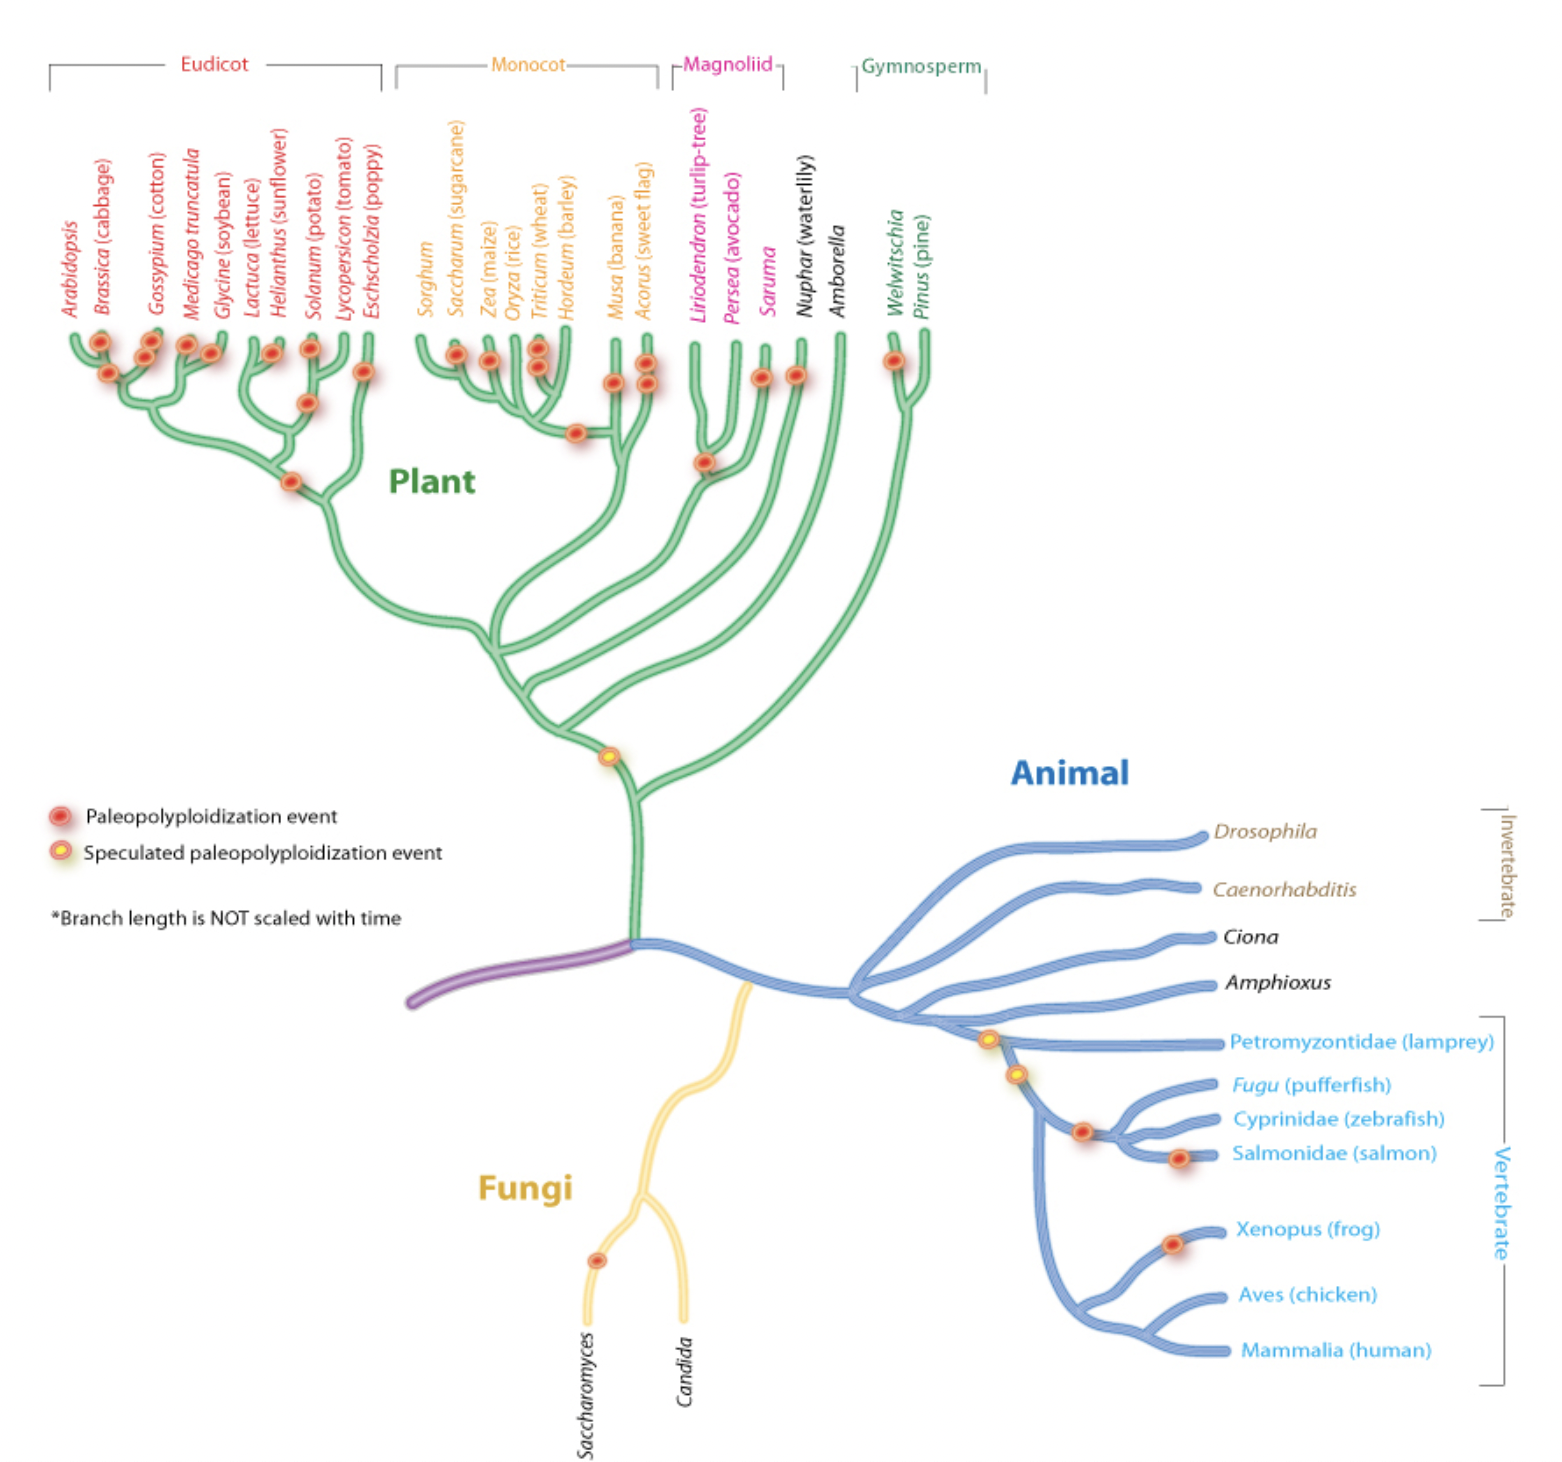
\includegraphics[width=0.7\linewidth]{figuras/PaleopolyploidyTree} 

}

\caption{Eventos de paleopoliploidías (poliploidías que datan de millones de años) en la evolución, con evidencia fuerte (puntos rojos) y eventos putativos (puntos amarillos). Figura extraída de Wikipedia, creada por Peter Zhang, (CC BY-SA 3.0)}\label{fig:PaleopolyploidyTree}
\end{figure}

En el caso diploide, el producto de dos paréntesis \((p+q)\) representa el
producto de dos eventos independientes: la generación de
gametos. En el caso de los organismos poliploides (pongamos por caso un
tetraploide), existe en primer lugar el proceso de sorteo aleatorio de qué par de alelos
terminarán en el mismo gameto, y luego la combinación de gametos para producir el cigoto. Es decir, en el caso del tetraploide hay 4
multiplicaciones de las frecuencias de los alelos \textbf{A} y \textbf{a}, por lo
que ahora la distribución de las frecuencias de los distintos genotipos
estará dada por

\begin{equation}
(f_{\bf{A}}+f_{\bf{a}})(f_{\bf{A}}+f_{\bf{a}})(f_{\bf{A}}+f_{\bf{a}})(f_{\bf{A}}+f_{\bf{a}})=(p+q)(p+q)(p+q)(p+q)=(p+q)^4
\end{equation}

Para el caso de un locus con dos alelos en una especie tetraploide, el
desarrollo de la fórmula anterior nos lleva a la distribución de las
frecuencias que se puede observar en el siguiente cuadro:

\begin{table}
\centering
\begin{tabular}[t]{ll}
\toprule
Genotipo & Frecuencia\\
\midrule
\cellcolor{gray!10}{$\textbf{AAAA}$} & \cellcolor{gray!10}{$p^4$}\\
$\textbf{AAAa}$ & $4p^3q$\\
\cellcolor{gray!10}{$\textbf{AAaa}$} & \cellcolor{gray!10}{$6p^2q^2$}\\
$\textbf{Aaaa}$ & $4pq^3$\\
\cellcolor{gray!10}{$\textbf{aaaa}$} & \cellcolor{gray!10}{$q^4$}\\
\bottomrule
\end{tabular}
\end{table}

Claramente esto es generalizable a otras ploidias, al menos a las pares
(recordar que las ploidias impares suelen tener problemas de
segregación), de acuerdo a

\begin{equationbox}
\begin{equation}
(f_{\bf{A}}+f_{\bf{a}})*...*(f_{\bf{A}}+f_{\bf{a}})=(p+q)*...*(p+q)=(p+q)^n
\end{equation}

\end{equationbox}

donde \(n\) corresponde a la ploidía (\(n=2\) para diploides, \(n=4\) para tetraploides, \(n=6\)
para hexaploides, etc.). Obviamente, al tratarse de un locus con dos
alelos, los coeficientes que aparecen en el cuadro de más arriba, y que surgen de la generalización, son los coeficientes del ``binomio de
Newton'', o lo que es equivalente del ``triángulo de Pascal'' (o de
Tartaglia, pese a que el desarrollo del mismo claramente antecede a
ambos).

\begin{graybox}

Al estimar frecuencias en un sistema de un \emph{locus} con dos alelos:

\begin{itemize}
\tightlist
\item
  Si suponemos que los individuos representan un muestreo al azar de los gametos en la población y que los individuos de la muestra fueron seleccionados al azar, entonces la probabilidad de observar un conteo \(x\) en particular, dado el número total de alelos genotipados \(n\), se puede describir por la distribución binomial: \(f(x)={n\choose x} p^x (1-p)^{n-x}\), con las combinaciones de \(n\) elementos tomados de a \(x\) elementos dados por \({n\choose x}=\frac{n!}{x!(n-x)!}\)
\end{itemize}

Equilibrio de Hardy-Weinberg en especies poliploides:

\begin{itemize}
\item
  A modo de ejemplo, en el caso de organismos tetraploides hay 4 multiplicaciones de las frecuencias de los alelos \textbf{A} y \textbf{a}, por lo que ahora la distribución de las frecuencias de los distintos genotipos será dada por \((p+q)^4\).
\item
  Esto es generalizable a otras ploidias, al menos a las pares de acuerdo a
  \((f_{\bf{A}}+f_{\bf{a}})*...*(f_{\bf{A}}+f_{\bf{a}})=(p+q)*...*(p+q)=(p+q)^n\)
\end{itemize}

\end{graybox}

\section{\texorpdfstring{Geometría y Genética: los diagramas de \emph{de Finetti}}{Geometría y Genética: los diagramas de de Finetti}}\label{geometruxeda-y-genuxe9tica-los-diagramas-de-de-finetti}


\includegraphics[width=0.13\textwidth,height=\textheight]{figuras/topicoav.png}

Aunque nos pueda parecer algo extraño, existe una fuerte conexión entre
genética y geometría. De hecho, como veremos más adelante, Sewall Wright \footnote{Sewall Green Wright (21 de diciembre, 1889 - 3 marzo, 1988), fue
  un genetista que realizó notables aportes sobre los efectos de la
  selección y la deriva, así como el análisis de pequeñas poblaciones
  y el efecto de la consanguinidad . Junto a Ronald A. Fisher y JBS
  Haldane establecieron la fundación matemática de la genética de
  poblaciones y de la teoría evolutiva.} imaginó la evolución como un paisaje adaptativo, con
picos y valles por los que se movían las poblaciones (\citeproc{ref-Wright1932}{S. Wright 1932}), lo que conecta
mentalmente de inmediato a un mundo de formas geométricas. Sin embargo,
ya antes de esa fecha, Bruno de Finetti (\citeproc{ref-deFinetti1926}{Finetti 1926}) había
establecido que gran parte de los mecanismos y resultados de la genética
mendeliana se podían obtener de consideraciones geométricas. Uno de los
aportes más relevantes en este sentido es la idea de que para un locus
con dos alelos en una especie diploide es posible representar todas las
combinaciones posibles de las frecuencias genotípicas como los puntos
interiores de un triángulo equilátero. Para ello, de Finetti hace uso del
resultado del teorema de Viviani, por lo que primero veremos en primer lugar qué establece
dicho teorema.\\
El teorema de Viviani \footnote{Vincenzo Viviani (5 de abril,1622 - 22 de setiembre, 1703),
  matemático y científico italiano, pupilo de Torricelli y discípulo
  de Galileo.} establece que, para triángulos equiláteros, la
suma de las distancias desde cualquier punto interno del mismo a los
tres lados es igual a la altura del triángulo. Para demostrarlo nos
basaremos en el esquema de la Figura \ref{fig:Viviani}, donde dentro
del triángulo de vértices \textbf{A}, \textbf{B} y \textbf{C}, con altura \(h\) y lado
\(a\), tenemos al punto \textbf{P}.

\begin{figure}[H]

{\centering 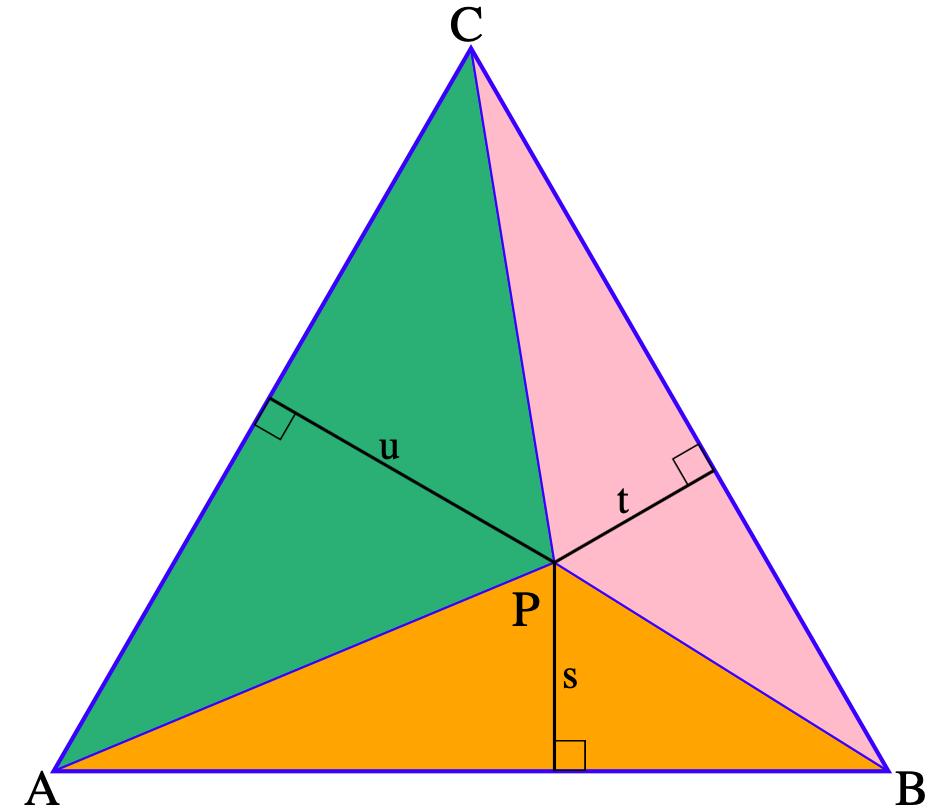
\includegraphics[width=0.6\linewidth]{figuras/Viviani_theorem} 

}

\caption{Triángulo usado para demostrar el teorema de Viviani. Figura tomada de Wikipedia, CC0 (Archivo:Viviani Theorem.svg).}\label{fig:Viviani}
\end{figure}

Llamemos \textbf{s}, \textbf{t} y \textbf{u} a las
distancias de \textbf{P} a los lados \(\overline{\rm AB}\), \(\overline{\rm BC}\)
y \(\overline{\rm CA}\), respectivamente, que son las alturas (por
definición) de los tres triángulos internos de vértices \textbf{APB}, \textbf{BPC}
y \textbf{CPA}. Estos triángulos, a su vez completan toda el área del
triángulo de vértices \textbf{ABC}. Como el área de un triángulo es igual a
\(\frac{\text{base} \cdot \text{altura}}{2}\), tenemos entonces que

\begin{equation}
\frac{a.s}{2}+\frac{a.t}{2}+\frac{a.u}{2}=\frac{a.h}{2} \Leftrightarrow \frac{a}{2}(s+t+u)=\frac{a}{2} h \Leftrightarrow s+t+u=h
\end{equation}

por lo que queda demostrado este teorema. Dicho de otra manera, la
significación de este teorema es que para cualquier punto interno a un
triángulo equilátero, la suma de distancias a los lados es constante e
igual a la altura del triángulo.\\

Veamos ahora cómo se relaciona este teorema con la genética. Supongamos
que tenemos un locus con dos alelos. Asignamos los tres genotipos
posibles a los vértices de un triángulo equilátero de altura igual a 1.
Sin pérdida de generalidad, pongamos por ejemplo los homocigotas en la
base (es un triángulo equilátero, por lo que todos sus lados son
iguales) como muestra la Figura \hyperref[deFinetti]{2.10}.

\begin{figure}[H]

{\centering 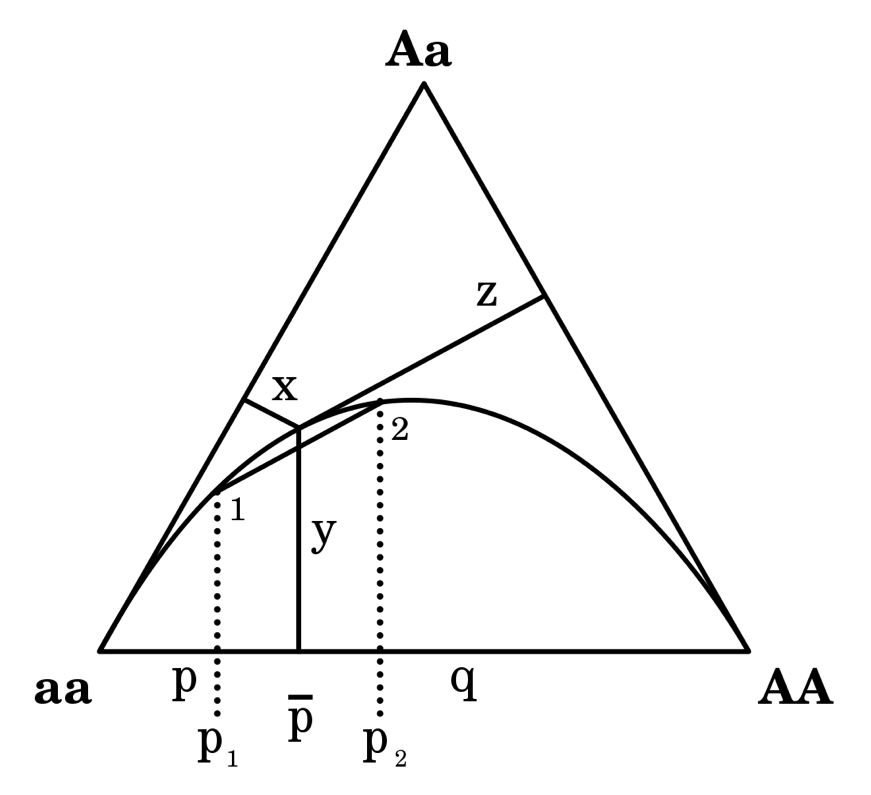
\includegraphics[width=0.6\linewidth]{figuras/deFinetti_diagram} 

}

\caption{Diagrama de de Finetti.Figura tomada de Wikipedia, CC BY-SA 2.5 (Archivo:De Finetti diagram.svg).}\label{fig:deFinetti}
\end{figure}

Denotamos \(p\) a la frecuencia del alelo \(A\) y \(q=1-p\) la
frecuencia del alelo \(a\). Ahora, de acuerdo al teorema de Viviani,
sabemos que para cualquier punto interno del tríangulo la suma de
distancias a los lados es igual a 1 (la altura del triángulo). Pero, ¿qué representan estas
distancias? Para entender este punto, imaginemos primero que
estamos en el vértice \textbf{AA} (abajo a la derecha): ahora la distancia de
este punto hasta el lado opuesto es igual a 1; lo mismo ocurrirá con los otros dos vértices. Es decir que cuando
estamos en algún vértice, la distancia al lado opuesto es igual a 1, o
lo que es lo mismo, la frecuencia del correspondiente genotipo es de 1
(todos los individuos son de ese genotipo). Tenemos entonces que cada distancia a
un lado del triángulo representa la frecuencia del genotipo en el
vértice opuesto. A medida de que nos apartamos de los vértices comienzan a aparecer distancias no nulas a los dos otros lados, además de al lado opuesto al vértice. Esto se ve gráficamente en la Figura \ref{fig:deFinetti}, donde las distancias \textbf{x}, \textbf{y} y \textbf{z}
representan las frecuencias de los genotipos \textbf{AA},
\textbf{Aa} y \textbf{aa}, respectivamente. Que la suma de las frecuencias de los genotipos sea
igual a 1 está garantizado por el teorema de Viviani.

Más aún, el punto de intersección de la distancia \textbf{y} con el eje
formado por los vértices \textbf{AA} y \textbf{aa} separa a este lado en dos
segmentos; el de la izquierda es proporcional a la frecuencia del alelo
\textbf{A} (\(p\)), mientras que el de la derecha es proporcional a la frecuencia
del alelo \textbf{a} (\(p=1-q\)). La distancia \textbf{y} representa la frecuencia
de los heterocigotas (\textbf{Aa}) y, como ya vimos previamente (Sección \hyperref[heterocigotas-freq-alelica]{H-W: la frecuencia de heterocigotas en función de la frecuencia alélica}), bajo
equilibrio de Hardy-Weinberg la misma describe una parábola en función
de la frecuencia del alelo \textbf{A} (\(p\), o en forma alternativa del otro
alelo). Por lo tanto, el equilibrio de Hardy-Weinberg se encuentra
representado en la Figura \ref{fig:deFinetti} por la curva que va desde el vértice \textbf{aa} al
vértice \textbf{AA}. Es decir, solo los puntos que se encuentran en esta
curva (y por lo tanto las distancias asociadas a los lados) representan
configuraciones de genotipos que se encuentran en equilibrio de
Hardy-Weinberg.

Un ejemplo de la utilidad de lo anterior es la demostración visual de un
efecto que veremos más adelante: la unión de (los individuos de) dos
poblaciones en equilibrio de Hardy-Weinberg usualmente no produce una
población conjunta en equilibrio H-W (antes de la reproducción). Esto suele resultar en la deficiencia en el número de heterocigotos
respecto a la frecuencia esperada del promedio de las frecuencias
alélicas en las dos poblaciones. Para ver esto en la Figura
\ref{fig:deFinetti}, supongamos que tenemos dos poblaciones \textbf{1} y \textbf{2} (del mismo tamaño)
que se encuentran en equilibrio H-W, y por lo tanto son puntos sobre la
curva. La frecuencias del alelo \textbf{A} en cada una de esta poblaciones
será el segmento de recta izquierdo en el eje entre los vértices \textbf{AA}
y \textbf{aa}, \(p_1\) y \(p_2\), cuyo promedio es \(\bar p\). Si ahora subimos
\(\bar p\) hasta la curva de equilibrio, vemos que la intersección con el
segmento de recta que une los puntos \textbf{1} y \textbf{2} (el promedio de las
frecuencias genotípicas entre estas poblaciones) ocurre antes que con la
curva. Lo que es equivalente, la distancia que representa la
frecuencia promedio de los heterocigotas es menor a la que representa el valor esperado bajo equilibrio de Hardy-Weinberg.

Un análisis más exhaustivo sobre las posibilidades del diagrama de
Finetti se encuentra en Cannings and Edwards (\citeproc{ref-pmid5673165}{1968}), donde por ejemplo los autores
muestran que la endocría (``\emph{inbreeding}'', concepto que veremos también más
adelante) produce una parábola por debajo de la que corresponde al
equilibrio de H-W, mientras que los procesos de selección producen una
serie de ``cónicas'' (curvas resultantes de cortar un cono variando el
ángulo del plano de corte) que también pasan por los vértices \textbf{AA} y
\textbf{aa}.

\section{La estimación de frecuencias en el locus ABO}\label{estimacion-abo}


\includegraphics[width=0.13\textwidth,height=\textheight]{figuras/topicoav.png}

Los métodos elaborados para la estimación de las frecuencias hacen
uso del concepto de máxima verosimilitud, pero (\citeproc{ref-pmid6598211}{Yasuda 1984}) propuso un
método sencillo basado en conteo. Supongamos que \(T=A+B+AB+O\), es decir
el total de individuos de los distintos fenotipos. Trabajaremos con la
determinación de \(p\), la frecuencia del alelo \(I^A\), pero para \(q\) (la
frecuencia del \(I^B\)) la situación es idéntica por simetría y basta con
sustituir A por B e \(I^A\) por \(I^B\). La frecuencia del alelo \(I^A\) será
igual a la cantidad total de alelos \(I^A\) en los fenotipos que tienen
este alelo, es decir A (\(I^AI^A\)) y AO (\(I^Ai\)) que solo expresan el A,
más el AB (\(I^AI^B\)) que expresa los dos alelos, todo dividido entre
\(2T\) que es el número total de alelos en los individuos. En el primer
caso hay dos alelos \(I^A\) por cada individuo, mientras que en los otros
dos hay solo un alelo por individuo. Sin embargo, nosotros no podemos
distinguir los 3 fenotipos, ya que tanto el A como el AO solo expresan
el alelo \(I^A\), por lo que debemos buscar una forma de separar el aporte
de cada uno de estos genotipos al conteo. Mientras que el \(I^Ai\) aporta
un alelo \(I^A\), el \(I^AI^A\) aporta dos alelos, por lo que todos los
fenotipos A aportarán un alelo, mientras que una cierta fracción (los
homocigotos) aportará un segundo alelo también. ¿Cuál es la fracción
del fenotipo A que corresponde a los homocigotas \(I^AI^A\)? De acuerdo a
lo predicho por el equilibrio de Hardy-Weinberg, los homocigotas
\(I^AI^A\) serán \(p^2\), mientras que los heterocigotas \(I^Ai\) serán \(2pr\),
por lo que la fracción de homocigotas \(h_A\) será

\begin{equation}
h_A=\frac{p^2}{p^2+2pr}=\frac{p^2}{p(p+2r)}=\frac{p}{p+2r}
\label{eq:hA}
\end{equation}

Es decir, si sumamos las contribuciones de AB, todos los A y el resto de
los A homocigotos, tenemos

\begin{equation}
p=\frac{[AB+A+Ah_A]}{2T}
\label{eq:pYasuda}
\end{equation}

Si definimos a partir de los fenotipos observables A y O, \(k_A=O/(A+O)\), entonces podemos expresar
\(k_A\) en términos de lo esperable bajo equilibrio Hardy-Weinberg como

\begin{equation}
\begin{split}
k_A=\frac{Tr^2}{T(p^2+2pr)+Tr^2}= \frac{r^2}{p^2+2pr+r^2}=\frac{r^2}{(p+r)^2}=[r/(p+r)]^2\\
\therefore \sqrt{k_A}=\frac{r}{(p+r)}
\end{split}
\label{eq:kA}
\end{equation}

¿Cuál es la relación entre \(h_A\) y \(k_A\)? Usando las definiciones de \(h_A\) (ecuación \eqref{eq:hA}) y \(k_A\) (ecuación \eqref{eq:kA}), tenemos que

\begin{equation}
\begin{split}
h_A=\frac{p}{p+2r}=\frac{p+r-r}{p+r+r}=\frac{\frac{p+r-r}{p+r}}{\frac{p+r+r}{p+r}}=\frac{\frac{p+r}{p+r}-\frac{r}{p+r}}{\frac{p+r}{p+r}+\frac{r}{p+r}}=\\
=\frac{1-\frac{r}{p+r}}{1+\frac{r}{p+r}}=\frac{1-\sqrt{k_A}}{1+\sqrt{k_A}}\\
h_A=\frac{1-\sqrt{k_A}}{1+\sqrt{k_A}}=\frac{(1-\sqrt{k_A})}{(1+\sqrt{k_A})} \frac{(1-\sqrt{k_A})}{(1-\sqrt{k_A})}=\\
=\frac{(1-\sqrt{k_A})^2}{1-k_A}
\end{split}
\label{eq:hAkA}
\end{equation}

¡Excelente! Tenemos la relación entre \(h_A\) y \(k_A\) (expresada de dos
formas), pero aún nos falta llegar a una forma de \(h_A\) que sea una
función de cantidades observables, es decir los fenotipos. Si recordamos
la definición de \(k_A\) a partir de los fenotipos observables
(\(k_A=O/(A+O)\)) y sustituimos en la ecuación
\eqref{eq:hAkA}, tenemos

\begin{equation}
\begin{split}
h_A=\frac{(1-\sqrt{k_A})^2}{1-k_A}  \Leftrightarrow  h_A (1-k_A)=(1-\sqrt{k_A})^2 \Leftrightarrow h_A (1-\frac{O}{A+O})=1-2\sqrt{k_A}+k_A
\end{split}
\end{equation}

Llevando todo a denominador \(A+O\), tenemos

\begin{equation}
\begin{split}
h_A (\frac{A+O}{A+O} - \frac{O}{A+O}) =  h_A (\frac{A+O-O}{A+O})=1-2 \cdot \sqrt{\frac{O}{A+O}}+\frac{O}{A+O} \Leftrightarrow \\ h_A (\frac{A}{A+O})=\\=\frac{A+O}{A+O} - \frac{\sqrt{A+O}}{\sqrt{A+O}} \cdot 2 \cdot \frac{\sqrt{O}}{\sqrt{A+O}}+\frac{O}{A+O}\\h_A (\frac{A}{A+O})=\frac{(A+O)-2\sqrt{O(A+O)}+O}{A+O} \Leftrightarrow \\ Ah_A (\frac{O}{A+O})\cdot (A+O) = A+O-2\sqrt{O(A+O)}+O \\Ah_A=A+O-2\sqrt{O(A+O)}+OAh_A \therefore \\Ah_A  = A+2O-2\sqrt{O(A+O)}
\end{split}
\end{equation}

Finalmente, si volvemos al principio con este resultado y sustituimos en
\eqref{eq:pYasuda}, tenemos el estimador basado en conteo

\begin{equation}
\begin{split}
\hat{p}=\frac{[AB+A+Ah_A]}{2T}=\frac{[AB+A+(A+2O-2\sqrt{O(A+O)})]}{2T} \therefore \\
\hat{p}=\frac{[(1/2)AB+A+O-\sqrt{O(A+O)}]}{T}
\end{split}
\end{equation}

Analogamente, por simetría, para la estimación de \(q\) tenemos

\begin{equation}
\hat{q}=\frac{[(1/2)AB+B+O-\sqrt{O(B+O)}]}{T}
\end{equation}

y por lo tanto, \(\hat{r}=1-\hat{p}-\hat{q}\). Sencillo, ¿no?

\subsubsection*{Ejemplo 2.4}\label{ejemplo-2.4}
\addcontentsline{toc}{subsubsection}{Ejemplo 2.4}

Entre donantes de sangre de la ciudad de Ankara
(Turquía) se determinó que de 1500 donantes sanos se observaron 669 del
grupo A, 484 del grupo O, 232 del grupo B y 115 del grupo AB. Utilizando
los estimadores que propuso (\citeproc{ref-pmid6598211}{Yasuda 1984}) estimar las frecuencias de
los alelos \(I^A\), \(I^B\) e \(i\), así como el número esperado de los
distintos fenotipos si la población estuviese en equilibrio de
Hardy-Weinberg.\\

\begin{equation*}
\begin{split}
\hat{p}=\frac{[(1/2)AB+A+O-\sqrt{O(A+O)}]}{T}=\frac{((115/2)+669+484-\sqrt{(484(669+484))})}{1500}=0,3089808 \\
\hat{q}=\frac{[(1/2)AB+B+O-\sqrt{O(B+O)}]}{T}=\frac{((115/2)+232+484-\sqrt{(484(232+484))})}{1500}=0,1232134 \\
\hat{r}=1-\hat{p}-\hat{q}=1-0,3089808-0,1232134=0,5678058
\end{split}
\end{equation*}

De acuerdo a las frecuencias estimadas previamente, el número esperado
de cada fenotipo sería

\begin{equation*}
\begin{split}
E(A)=(p^2+2pr)T=(0,3089808^2+2\cdot 0,3089808\cdot 0,5678058)\cdot 1500=669,527
\sim 670\\
E(B)=(q^2+2qr)T=(0,1232134^2+2\cdot 0,1232134\cdot 0,5678058)\cdot 1500=232,6562
\sim 233\\
E(AB)=2pqT=2\cdot 0,3089808\cdot 0,1232134\cdot 1500=114,2117 \sim 114 \\
E(O)=r^2T=0,5678058^2\cdot 1500=483,6051=484,
\end{split}
\end{equation*}

lo que coincide estrechamente con los números observados, por lo que \textbf{no podemos descartar que la población se encuentre en equilibrio Hardy-Weinberg} (en general no podemos resolver a favor de una hipótesis alternativa basados en la estadística, a lo sumo podemos afirmar que la misma es completamente improbable dados los supuestos del test que aplicamos).

\section{Conclusión}\label{conclusiuxf3n-1}

En este capítulo planteamos un modelo matemático básico, el equilibrio de Hardy-Weinberg, para realizar predicciones sobre las frecuencias genotípicas observadas en una población partiendo de las frecuencias alélicas existentes en la misma. A su vez observamos cómo el modelo es fácilmente ajustable a distintas situaciones de interés biológico. Las asunciones del modelo pueden resultar muy poco realistas (¿qué población natural tiene tamaño infinito?, ¿dónde se vió que los individuos se apareen al azar?). Si bien esto puede parecer una debilidad del modelo, en capítulos posteriores veremos cómo el equilibrio de Hardy-Weinberg puede utilizarse como una hipótesis nula para contrastar si es viable plantear que una población natural se comporta o no bajo alguna de las premisas del modelo. Gracias a su simpleza, el modelo resulta una excelente puerta de entrada al uso de la matemática para el estudio de la genética de poblaciones, aproximación de la que nos seguiremos nutriendo en lo que resta de este libro.

\newpage

\section{Actividades}\label{actividades-1}

\subsection{Control de lectura}\label{control-de-lectura-1}

\begin{enumerate}
\def\labelenumi{\arabic{enumi}.}
\tightlist
\item
  Varias de las asunciones necesarias para que se cumpla el modelo de equilibrio de Hardy-Weinberg no parecen ser realistas. ¿Cuál es la utilidad del modelo, si esto es así? Plantee al menos un ejemplo donde se viole alguna de las asunciones del modelo, y discuta la utilidad del modelo en dicho caso.
\item
  Describa qué sucede con las frecuencias alélicas esperadas en una población cuando existen diferentes proporciones de individuos machos y hembras.
\item
  A medida que aumenta el número de alelos presentes en una población en equilibrio de Hardy-Weinberg, aumenta necesariamente el número de genotipos heterocigotas en la misma. En estos casos, ¿cómo se puede calcular de forma sencilla la heterocigosidad esperada en la población, sin necesidad de sumar todas las frecuencias de genotipos heterocigotas?
\item
  Si un \emph{locus} se ve asociado a un cromosoma sexual, ¿se comporta igual que un \emph{locus} autosómico? Describa qué dinámica espera para las frecuencias alélicas en machos y hembras, así como el valor esperado para la frecuencia alélica a largo plazo en la población.
\item
  Las frecuencias alélicas deben ser estimadas a través de muestreos cuando se realiza un estudio poblacional.
  a. ¿En qué medida afectan los tamaños muestrales en este contexto?
  b. Nombre al menos un método que permita la determinación de los alelos presentes en un individuo muestreado.
\end{enumerate}

\subsection{¿Verdadero o falso?}\label{verdadero-o-falso-1}

\begin{enumerate}
\def\labelenumi{\arabic{enumi}.}
\tightlist
\item
  Si se cambian las frecuencias alélicas \(p\) y \(q\) de una población que se encuentra en equilibrio Hardy-Weinberg, las mismas se ajustarán en la próxima generación y volverán a su valor inicial (lo cual implica que las frecuencias genotípicas permanecerán invariables). A esta propiedad es que alude la palabra ``equilibrio''.
\item
  El modelo de equilibrio de Hardy-Weinberg predice que un alelo que sea letal en homocigosis no será eliminado de una población si el fenotipo heterocigota es indistinguible del resto de los fenotipos homocigotas.
\item
  La suma de las frecuencias genotípicas en una población que segrega un locus bi-alélico (con frecuencias \(p\) y \(q\)) siempre cumple con la ecuación \(p^2 + 2pq + q^2 = 1\).
\item
  Para un locus bi-alélico, la máxima heterocigosidad esperada corresponde al caso donde ambas frecuencias alélicas son iguales.
\item
  Si dos poblaciones se encuentran bajo equilibrio de Hardy-Weinberg, una población constituída por ambas también lo hará.
\end{enumerate}

\textbf{\emph{Solución}}

\begin{enumerate}
\def\labelenumi{\arabic{enumi}.}
\item
  \textbf{Falso}. Un cambio en las frecuencias alélicas llevará a un cambio de las frecuencias genotípicas esperadas bajo equilibrio de Hardy-Weinberg. La palabra ``equilibrio'' refiere al hecho de que, una vez establecidas estas frecuencias genotípicas, las mismas permenecerán iguales si las condiciones no cambian.
\item
  \textbf{Verdadero}. A medida que la frecuencia del alelo disminuye, el modelo prevé una prevalencia del alelo en los individuos heterocigotas (los cuales no son eliminados, ya que su fenotipo no sufre los efectos de cargar con el alelo). El alelo por tanto no es erradicado de la población.
\item
  \textbf{Falso}. Es correcto que la suma de las frecuencias genotípicas en una población debe equivaler a 1, ya que la suma de todas las frecuencias equivale al total de los casos posibles. No obstante, la ecuación \(p^2 + 2pq + q^2 = 1\) sólo será correcta si la población se encuentra bajo equilibrio de Hardy-Weinberg, ya que en dicho caso las frecuencias de genotipos homocigotas y heterocigotas se encuentran reflejadas en la ecuación.
\item
  \textbf{Verdadero}. En efecto, este caso implica que las frecuencias alélicas sean \(p=q=0,5\), con una hetercigosidad esperada de \(2 \cdot 0,5 \cdot 0,5 =0,5\). Ver sección de Ejercicios, donde se propone demostrar esta propiedad mencionada en el texto del capítulo.
\item
  \textbf{Falso}. La población total no se encontrará bajo equilibrio de Hardy-Weinberg. La causa de fondo es que los individuos de cada una de las poblaciones no se aparean con los de la otra (\emph{i.e.}, no existe panmixia en la población total). Un calculo sencillo muestra que existirá un déficit de heterocigotas (lo cual es observable en los diagramas de \emph{de Finetti}). Ahondaremos en este fenómeno en el capítulo \hyperref[aparnoalazar]{Apareamientos no-aleatorios}.
\end{enumerate}

\subsection*{Ejercicios}\label{ejercicios-2}
\addcontentsline{toc}{subsection}{Ejercicios}

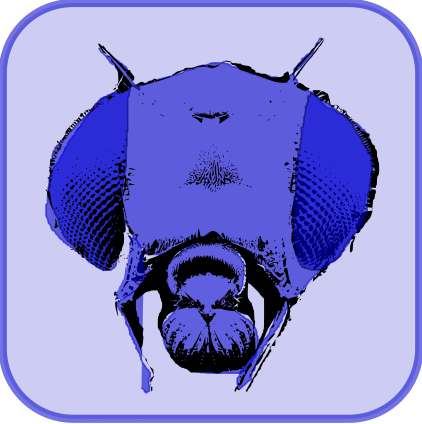
\includegraphics[width=0.06\textwidth,height=\textheight]{figuras/cabezamosca.png} \(\raisebox{2.5ex}{\textbf{Ejercicio 2.1}}\)

Un locus A posee dos alelos conocidos (\(A_1\) y \(A_2\)), los cuales segregan en dos poblaciones independientes de organismos diploides. Las poblaciones tienen tamaños \(N_1 = N\) y \(N_2 = 2N\), respectivamente. Las frecuencias genotípicas en las poblaciones son

\[
\begin{cases}
f_1(A_1A_1) = 0,36;\ f_1(A_1A_2) = 0,48;\ f_1(A_2A_2) =  0,16 \\
f_2(A_1A_1) = 0,09;\ f_2(A_1A_2) = 0,42;\ f_2(A_2A_2) = 0,49
\end{cases}
\]

Se asume que en ambos casos el locus segrega acorde a lo esperado bajo equilibrio de Hardy-Weinberg. Calcule las frecuencias genotípicas esperadas si se unen las poblaciones.

\textbf{\emph{Solución}}

Para poder calcular las frecuencias genotípicas esperadas bajo equilibrio de Hardy-Weinberg, debemos calcular las nuevas frecuencias alélicas en la población resultante de la unión de ambas poblaciones, las cuales llamaremos \(f_T(A_1)\) y \(f_T(A_2)\). Una vez obtenidos estos valores, podemos proceder a calcular las frecuencias genotípicas esperadas.

La frecuencia alélica \(f_T(A_1)\) corresponde a
\[f_T(A_1) = \frac{\text{Núm. alelos }A_1}{\text{Núm. total de alelos}} = \frac{(2N_1 \cdot f_1(A_1)) + (2N_2 \cdot f_2(A_1))}{2N_1 + 2N_2}\]

donde \(f_1(A_1) = f_1(A_1A_1) + \frac{1}{2}\cdot f_1(A_1A_2)\) y \(f_2(A_1) = f_2(A_1A_1) + \frac{1}{2}\cdot f_2(A_1A_2)\).

Sustituyendo, tenemos

\[
f_T(A_1) = \frac{(2N_1 \cdot [f_1(A_1A_1) + \frac{1}{2}\cdot f_1(A_1A_2)]) + (2N_2 \cdot [f_2(A_1A_1) + \frac{1}{2}\cdot f_2(A_1A_2)])}{2N_1 + 2N_2}\] \[f_T(A_1) = \frac{(2N \cdot [f_1(A_1A_1) + \frac{1}{2}\cdot f_1(A_1A_2)]) + (2(2N) \cdot [f_2(A_1A_1) + \frac{1}{2}\cdot f_2(A_1A_2)])}{2N + 2(2N)}
\]

\begin{equation}
f_T(A_1) = \frac{(2 N \cdot [0,36 + \frac{1}{2}\cdot 0,48]) + (2(2 N) \cdot [0,09 + \frac{1}{2}\cdot 0,42])}{2N + 2(2 N)} 
\end{equation}

\[f_T(A_1) = 0,4\]

Por analogía, se puede calcular \(f_T(A_2)\). A su vez, se puede considerar que \(f_T(A_1) + f_T(A_2) = 1 \Rightarrow f_T(A_2) = 1 - f_T(A_1) = 1 - 0,4 = 0,6\)

De esto se desprende que

\[
\begin{cases}
f_T(A_1A_1) = 0,4^2 = 0,16 \\
f_T(A_1A_2) = 2 \cdot 0,4 \cdot  0,6 = 0,48 \\
f_T(A_2A_2) = 0,6^2 = 0,36
\end{cases}
\]

\hfill\break

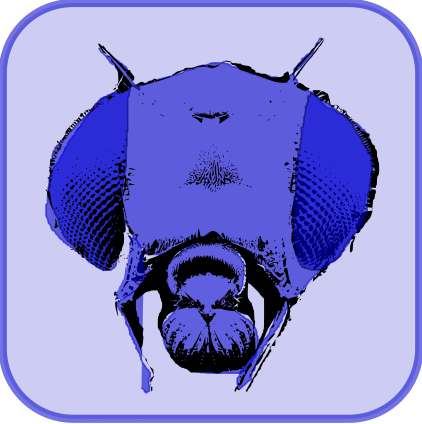
\includegraphics[width=0.06\textwidth,height=\textheight]{figuras/cabezamosca.png} \(\raisebox{2.5ex}{\textbf{Ejercicio 2.2}}\)

Dos poblaciones independientes de igual tamaño (\(N\)) se encuentran divididas por una barrera geográfica que impide la reproducción entre organismos de ambos lugares. Las poblaciones segregan un locus \(A\) con tres alelos conocidos (\(A_1\), \(A_2\) y \(A_3\)), acorde a lo esperado en equilibrio de Hardy-Weinberg.
Las poblaciones presentan las siguientes frecuencias genotípicas:

\[
\begin{cases}
f_1(A1) = 0,6; f_1(A_2) = 0,4; f_1(A_3) = 0 \\
f_2(A1) = 0; f_2(A_2) = 0,3; f_2(A_3) = 0,7 
\end{cases}
\]

En un momento dado se desaparece la barrera geográfica que dividen a las poblaciones, pasándose a un régimen de panmixia para la población resultante.

\textbf{a.} Calcule el promedio de la heterocigosidad de las poblaciones, previa a la ruptura de las barrera geográficas.

\textbf{b.} Calcule la heterocigosidad en la población resultante de la unión de las poblaciones, asumiendo que esta cumple con las asunciones del equilibrio Hardy-Weinberg.

\textbf{c.} ¿Son iguales los valores obtenidos en a y b? Vincule su respuesta a las asunciones del equilibrio Hardy-Weinberg.

\textbf{\emph{Solución}}

\textbf{a.} Calculamos la heterocigosidad esperada en cada caso:
\[H_1 = 2 \cdot 0,6 \cdot 0,4 = 0,48\]
\[H_2 = 2 \cdot 0,7 \cdot 0,3 = 0,42\]

de esto se desprende
\[\overline{H} = \frac{H_1 + H_2}{2} = \frac{0,48 + 0,42}{2} = 0,45\]

\textbf{b.} Primero debemos recalcular las frecuencias alélicas (\(f_T(A_i)\), para cada alelo \(i\)), a efectos de poder estimar frecuencias genotípicas bajo equilibrio de Hardy-Weinberg en la población total.

Tenemos que

\begin{equation}
\begin{cases}
f_T(A_1) = \frac{2 N \cdot 0,6 + 2 N \cdot 0}{2 N + 2 N} = \frac{0,6}{2} \\
f_T(A_2) = \frac{2 N \cdot 0,4 + 2 N \cdot 0,3}{2 N + 2 N} = \frac{0,4 + 0,3}{2} = \frac{0,7}{2} \\
f_T(A_3) = \frac{2 N \cdot 0,7 + 2 N \cdot 0}{2 N + 2 N} = \frac{0,7}{2}
\end{cases}
\end{equation}

Notemos que las frecuencias alélicas suman 1.

La heterocigosidad esperada se puede calcular a partir de la homocigosidad, notando que
\[H = 1 - \sum_{i=1}^{i=3} A_i^2\]

por lo que

\[H_T = 1 - (0,3^2 + 0,35^2 + 0,35^2)\]
\[H_T = 0,665\]

\textbf{c.} La heterocigosidad esperada bajo equilibrio Hardy-Weinberg para la población en conjunto es mayor al promedio de heterocigosidad entre ambas. Esto es de esperar (el lector puede referirse a la subsección \emph{2.10 Geometría y Genética: los diagramas de de Finetti} para una demostración visual del fenómeno). ¿A qué se debe esto? Una forma de aproximarse al problema es pensar desde el inicio en la población en su totalidad: bajo equilibrio de Hardy-Weinberg se asume panmixia, y los heterocigotas son producto del apareamiento al azar en la población. Cuando la población se estructura en dos o más grupos que sólo se reproducen entre sí (en nuestro caso, las poblaciones iniciales) se rompe este régimen de panmixia general, disminuyendo el número de heterocigotas producidos. Una forma clara de ver esto en el ejemplo planteado es que, cuando se consideran dos poblaciones, no se generan individuos heterocigotas \(A_1A_3\).

\hfill\break

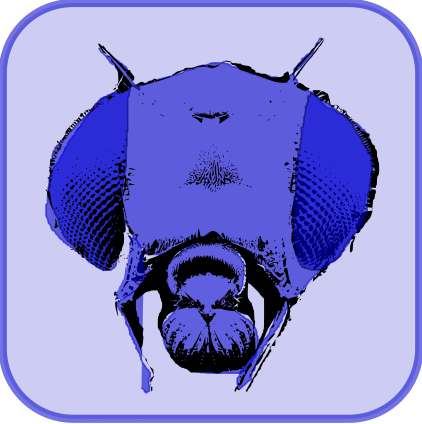
\includegraphics[width=0.06\textwidth,height=\textheight]{figuras/cabezamosca.png} \(\raisebox{2.5ex}{\textbf{Ejercicio 2.3}}\)

Un locus \(A\) presenta seis alelos que segregan acorde a lo esperado por el equilibrio Hardy-Weinberg.
Las proporciones alélicas son las siguientes:

\[
\begin{cases}
 f(A_1) = 0,15 \\
 f(A_2) = 0,25 \\
 f(A_3) = 0,3 \\
 f(A_4) = 0,09 \\
 f(A_5) = 0,2 \\
 f(A_6) = 0,01
\end{cases}
\]

\textbf{a.} Calcular la heterocigosidad esperada para el locus.

\textbf{b}. Durante un período las condiciones ambientales cambian, y se pierden todos los individuos con alelos \(A_4\), \(A_5\) y \(A_6\). Una vez reestablecido el equilibrio de Hardy-Weinberg, las proporciones alélicas son ahora

\[
\begin{cases}
f(A_1) = 0,1 \\
f(A_2) = 0,7 \\
f(A_3) = 0,2 \\
\end{cases}
\]

¿La heterocigosidad aumentó o disminuyó en la población? ¿Qué tanto respecto a lo obtenido en la primera parte del ejercicio?

\textbf{\emph{Solución}}

\textbf{a.} Recordemos que la frecuencia total de heterocigotas (heterocigosidad) se puede calcular a partir de la frecuencia total de homocigotas, en tanto la suma de ambas frecuencias debe sumar uno (ya que un organismo es o bien homocigota, o bien heterocigota).

Tenemos por tanto que

\[H = 1 - \sum_{i=1}^{i=6} A_i^2\]

por lo que

\[H = 1 - (0,15^2 + 0,25^2 + 0,3^2 + 0,09^2 + 0,2^2 + 0,01^2)\]
\[H = 0,7768\]

\textbf{b.} Aplicando la misma lógica, tenemos que en el nuevo escenario
\[H = 1 - (0,1^2 + 0,7^2 + 0,2^2) = 0,46\]

La heterocigosidad disminuyó. Aplicando un cociente, podemos expresar qué fracción del primer valor representa este nuevo valor de heterocigosidad. Llamaremos a estas heterocigosidades \(H_1\) y \(H_2\). Tenemos que

\[\frac{H_2}{H_1} = \frac{0,46}{0,7768} \approx 0,59\]

Vemos que la heterocigosidad disminuyó en el segundo escenario a casi el 60\% del valor planteado en primera instancia.

\hfill\break

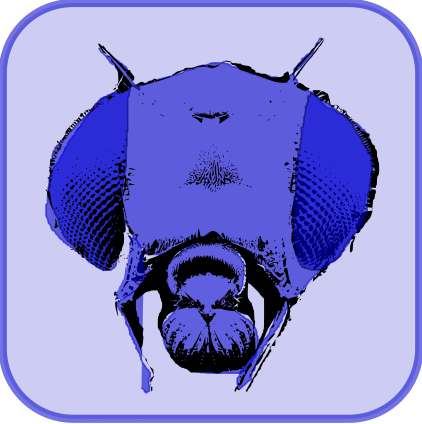
\includegraphics[width=0.06\textwidth,height=\textheight]{figuras/cabezamosca.png} \(\raisebox{2.5ex}{\textbf{Ejercicio 2.4}}\)

Dos loci bi-alélicos, \(A\) y \(B\), se encuentran segregando de forma independiente en una población de organismos diploides. Las frecuencias alélicas en la población son

\[
\begin{cases}
f(A_1) = 0,2 \\
f(A_2) = 0,8 \\
f(B_1) = 0,4 \\
f(B_2) = 0,6 \\
\end{cases}
\]

\textbf{a.} Realice un diagrama de Punnett mostrando los posibles genotipos en la población.

\textbf{b.} Calcule las frecuencias genotípicas esperadas bajo equilibrio de Hardy-Weinberg.

\textbf{\emph{Solución}}

\textbf{a.} Se muestran el cuadro de 16 combinaciones posibles, correspondientes a .

\textbf{b.} Los loci segregan de forma independiente, por lo que la presencia de un alelo de \(A\) no altera la probabilidad de encontrar un determinado alelo de \(B\). Se calculan las frecuencias genotípicas para cada locus, y la multiplicación de los mismos equivale a la frecuencia de organismos que los portarán los genotipos correspondientes en simultáneo

\[
\begin{cases}
f(A_1A_1) = 0,2^2; f(A_1A_2) = 2 \cdot 0,2 \cdot0,8; f(A_2A_2) = 0,8^2 \\
f(B_1B_1) = 0,4^2; f(B_1B_2) = 2\cdot0,4\cdot0,6; f(B_2B_2) = 0,6^2 
\end{cases}
\]

por lo que

\[
\begin{cases}
f(A_1A_1; B_1B_1) = 0,2^2 \cdot 0,4^2 = 0,0064 \\
f(A_1A_1; B_1B_2) = 0,2^2 \cdot (2 \cdot 0,4 \cdot 0,6) = 0,0192 \\
f(A_1A_1; B_2B_2) = 0,2^2 \cdot 0,6^2 = 0,0144 \\
f(A_1A_2; B_1B_1) = (2 \cdot 0,2 \cdot 0,8) \cdot 0,4^2 = 0,0512 \\
f(A_1A_2; B_1B_2) = (2 \cdot 0,2 \cdot 0,8) \cdot (2 \cdot 0,4 \cdot 0,6) = 0,1536 \\
f(A_1A_2; B_2B_2) = (2 \cdot 0,2 \cdot 0,8) \cdot 0,6^2 = 0,1152 \\
f(A_2A_2; B_1B_1) = 0,8^2 \cdot 0,4^2 = 0,1024 \\
f(A_2A_2; B_1B_2) = 0,8^2 \cdot (2 \cdot 0,4 \cdot 0,6) = 0,3072 \\
f(A_2A_2; B_2B_2) = 0,8^2 \cdot 0,6^2 = 0,2304
\end{cases}
\]\\


\includegraphics[width=0.06\textwidth,height=\textheight]{figuras/cienciabasica.png} \(\raisebox{2.5ex}{\textbf{Ejercicio 2.5}}\)

Un factor de transcripción (denotado por \(F\)) regula la expresión de un gen codificante para una enzima (denotada \(E\)) vinculada a la coloración en una especie diploide. Se asume que ambos loci segregan de forma independiente.

Los siguientes alelos son conocidos para estos loci
- Alelo \(F_a\): alelo codificante para una copia funcional del factor de transcripción.
- Alelo \(F_b\): alelo codificante para una copia disfuncional del factor de transcripción.
- Alelo \(E_a\): alelo codificante para una copia funcional de la enzima.
- Alelo \(E_b\): alelo codificante para una copia disfuncional de la enzima.

La presencia de una copia funcional para el factor de transcripción basta que el sistema sea funcional. En cambio, la coloración de los organismos depende del número de copias funcionales para la enzima \(E\): dos copias funcionales resultan en coloración roja, una copia funcional resulta en coloración rosada y la ausencia de copias funcionales resulta en ausencia de color.

\textbf{a.} Considere una población de tamaño \(N\), donde se tienen las siguientes frecuencias alélicas: \(f(F_a) = 0,5;\ f(E_a) = 1\). Describa la proporción de individuos que presentan coloración roja, rosada y nula en la población si se asume esta se encuentra en equilibrio de Hardy-Weinberg.

\textbf{b.} Considere una población de tamaño \(N\), donde se tienen las siguientes frecuencias alélicas: \(f(F_a) = 1;\ f(E_a) = 0,5\). Describa la proporción de individuos que presentan coloración roja, rosada y nula en la población si se asume esta se encuentra en equilibrio de Hardy-Weinberg.

\textbf{c.} Considere la población resultante de unificar las poblaciones anteriormente mencionadas. Describa la proporción de individuos que presentan coloración roja, rosada y nula en la población si se asume esta se encuentra en equilibrio de Hardy-Weinberg.

\textbf{\emph{Solución}}

\textbf{a.} La proporción de individuos que mostraran algún tipo de coloración corresponde a aquellos que preentan alguna copia funcional para el factor de transcripción \(F\). La proporción de individuos homocigotas \(F_bF_b\) para el alelo disfuncional está dada por \(f(F_b)^2 = 0,5^2 = 0,25\). Por lo tanto, la proporción de individuos que presentan coloración equivale a \(1-0,25 = 0,75\).
De estos, la totalidad portarán dos alelos \(E_a\), lo que resulta en coloración roja. Por lo tanto, se esperan las siguientes proporciones de coloración: \(f(\text{Rojo}) = 0,75, f(\text{Rosado}) = 0; f(\text{Albino}) = 0,25\).

\textbf{b.} La totalidad de los organismos serán homocigotas \(F_aF_a\) para el locus \(F\), por lo cual la coloración dependerá exclusivamente de las frecuencias esperadas de individuos \(E_aE_a\), \(E_aE_b\) y \(E_bE_b\) para el locus \(E\).
Tenemos que

\[
\begin{cases}
f(\text{Rojo}) = f(E_aE_a) = f(E_a)^2 = 0,5^2 = 0,25 \\
f(\text{Rosado}) = f(E_aE_b) + f(E_bE_a) = 2 \cdot f(E_a) \cdot f(E_b) = 2 \cdot 0,5 \cdot 0,5 = 0,5 \\
f(\text{Albino}) = f(E_bE_b) = f(E_b)^2 = 0,5^2 = 0,25
\end{cases}
\]

\textbf{\emph{c)}} El fenotipo de coloración dependerá tanto de los alelos presentes en el locus \(E\) como en el locus \(F\). Al combinar las poblaciones, las frecuencias alélicas (y genotípicas) cambiarán, y por lo tanto cambiará la proporción esperada para cada fenotipo. Los loci segregan de forma independiente, por lo cual podemos obtener las frecuencias genotípicas esperadas para cada locus por separado, y luego multiplicar las frecuencias resultantes para obtener las frecuencias esperadas en conjunto, las cuales correlacionan con los fenotipos esperados.
Para ello, primero necesitamos establecer las nuevas frecuencias alélicas \(f(F_a);\ f(F_b);\ f(E_a);\ f(E_b)\) para la población resultante.

Observemos qué pasa para un caso particular, el alelo \(F_a\):

\begin{equation}
f(F_a) = \frac{\text{núm. alelos }F_a}{2N + 2N} =  \frac{(2 N \cdot f_1(F_a) + 2(N \cdot f_2(F_a)))}{4 N} = \frac{2 \cdot 0,5 + 2 \cdot 1}{4} = 0,75
\end{equation}

Por analogía, se calculan las nuevas frecuencias alélicas en la población en el resto de los casos

\[
\begin{cases}
f(F_b) = 0,25 \\
f(E_a) = 0,75 \\
f(E_b) = 0,25
\end{cases}
\]

Por lo tanto, las frecuencias genotípicas esperadas en equilibrio Hardy-Weinberg para cada locus, son:

\[
\begin{cases}
f(F_aF_a) = 0,75^2;  f(F_aF_b) = 2 \cdot 0,75 \cdot 0,25; f(F_bF_b) = 0,25^2 \\
f(E_aE_a) = 0,75^2;  f(E_aE_b) = 2 \cdot 0,75 \cdot 0,25; f(E_bE_b) = 0,25^2
\end{cases}
\]

Considerando los dos genotipos al mismo tiempo, podemos dar las frecuencias fenotípicas esperadas para coloración.

\[
\begin{cases}
f(\text{Rojo}) = f(F_aF_a) \cdot f(E_aE_a) = 0,75^2 \cdot 0,75^2 \\
f(\text{Albino}) = f(F_bF_b;\ E_\text{.}E_\text{.})  + f(F_\text{.}F_\text{.}; E_bE_b) - f(F_bF_b;\ E_bE_b) = 0,25^2 + 0,25^2 - (0,25^2 \cdot 0,25^2)
\end{cases}
\]

en donde en el último caso restamos \(f(F_bF_b;\ E_bE_b)\) para no contar este genotipo dos veces.

Para facilitar los cálculos, notemos que los individuos que no sean rojos o albinos deberán ser necesariamente rosados, por la configuración del sistema. Esto nos da

\[f(\text{Rosado}) = 1 - (0,75^2 \cdot 0,75^2) - (0,25^2 + 0,25^2 - (0,25^2 \cdot 0,25^2)) \]
\[f(\text{Rosado}) = 0,5625 \]

Se puede verificar que esta frecuencia es equivalente a sumar las frecuencias de los genotipos que expresan este color.

\begin{center}\rule{0.5\linewidth}{0.5pt}\end{center}

\chapter{Deriva genética}\label{deriva}

En el capítulo anterior (\hyperref[variacion]{Variación y equilibrio de Hardy-Weinberg}) comenzamos a entender los procesos que hay por detrás del mantenimiento de la variabilidad genética en las poblaciones de distintas especies. En particular, a partir de las reglas mecanísticas de la herencia mendeliana\footnote{Gregor Mendel (20 de julio 1822 - 6 de enero de 1884) fue un meteorólogo, biólogo y matemático, nacido en Heizendorf bei Odrau, Imperio Austro-Húngaro (hoy República Checa). Considerado el padre de la ``genética moderna'', realizó diversos experimentos con plantas que lo llevaron a postular algunas ``leyes'', decenas de años antes de conocerse las bases moleculares de la herencia.} vimos que una vez alcanzado el equilibrio, si no aparecen otras fuerzas, las frecuencias alélicas y genotípicas se mantienen constantes generación tras generación. Para esto hemos asumido varias cosas (\hyperref[supuestos-que-asumimos-se-cumplen-para-h-w]{Supuestos que asumimos se cumplen para H-W}), algunas más razonables que otras. En particular, una de las cosas que asumimos es que el tamaño de nuestra población es prácticamente infinito (con esto queremos decir un número realmente muy alto de individuos), una situación que no siempre se cumple en la práctica. Más aún, esto nos lleva al concepto de población en nuestro contexto: el conjunto de individuos que potencialmente podrían aparearse en igualdad de condiciones con cualquier otro de la misma población para dejar descendencia fértil. Se trata de un concepto fácil de comprender, pero en la práctica suele ser bastante más complejo delimitar sus alcances. Pensemos, por ejemplo, en las poblaciones de Corriedale (ovinos), Angus (bovino de carne) o de Holando (bovino de leche) del Uruguay. ¿Se cumplen los supuestos del equilibrio de Hardy-Weinberg?. ¿Cuál sería mi población si el rebaño o rodeo es cerrado (\emph{i.e.}, produce sus propios reemplazos)?.

Habiendo definido en forma operativa lo que consideramos una población, rápidamente podemos llegar a ver que en muchas poblaciones asumir un tamaño casi infinito para las mismas es algo absurdo. Veremos que en las poblaciones donde se deja de lado esta asunción empieza a jugar una de las fuerzas siempre presentes en biología: el azar.\\

\begin{boxobjetivos}
\(\square\) Comprender como el azar puede ser una fuerza evolutiva de relevancia en poblaciones de tamaño finito.
\newline

\(\square\) Modelar este fenómeno a través de modelos matemáticos; esto nos permitirá derivar predicciones respecto a qué se espera de la evolución de las frecuencias alélicas en un conjunto de poblaciones iguales. En particular, veremos el modelo de Wright-Fisher y la aplicación de cadenas de Markov en este problema.
\newline

\(\square\) Describir la evolución de la homocigosidad en poblaciones de tamaño finito conforme pasan las generaciones. Se presentará al coeficiente de fijación, y su tendencia según el
modelo de Wright-Fisher.
\newline

\(\square\) Presentar el concepto de tamaño poblacional efectivo, el cual permite tratar a una población que se desvía de lo ideal con las herramientas matemáticas presentadas hasta ahora en dinstintos contextos biológicos.
\newline

\(\square\) Ver la aproximación por difusión, una herramienta matemática que permite integrar los procesos azarosos de cambio en las frecuencias alélicas con los procesos direccionados. Este modelado conjunto es más realista, en tanto en las poblaciones naturales es de esperar que los dos fenómenos tengan influencia.
\newline

\(\square\) Presentar el modelo de coalescente, un modelo clave en genética de poblaciones. Este nos permitirá nos permitirá indagar en la historia de una muestra de alelos, yendo hacia atrás en el tiempo (hasta identificar su último ancestro común en una población), estimando los tiempos esperados en el proceso.

\end{boxobjetivos}

\section{El rol de los procesos estocásticos en la genética}\label{el-rol-de-los-procesos-estocuxe1sticos-en-la-genuxe9tica}

Para estudiar el alcance del azar en nuestro contexto propongamos un experimento conceptual sencillo, que cada persona puede reproducir en su casa. Tomemos una jarra o vaso grande y coloquemos 20 bolitas de vidrio azules y 20 bolitas de vidrio rojas, \textbf{idénticas excepto por el color}. Si, como es de esperar, no tienes tantas bolitas de diferentes colores, alcanza con hacer bolitas de papel coloreado o cosas similares, aunque nosotros nos seguiremos refiriendo en nuestro ejemplo a las bolitas. Por lo tanto, el estado inicial de nuestro experimento (la jarra) es:

\begin{table}
\centering
\begin{tabular}[t]{lll}
\toprule
 & Azul & Roja\\
\midrule
\cellcolor{gray!10}{Cantidad} & \cellcolor{gray!10}{20} & \cellcolor{gray!10}{20}\\
Proporción & $\frac{20}{40}$ & $\frac{20}{40}$\\
\bottomrule
\end{tabular}
\end{table}

Si sacas una bolita sin mirar el color, ¿qué esperas que ocurra? ¿Será roja o será azul? La extracción de una bolita de nuestra jarra se trata de un fenómeno aleatorio (no podemos saber el resultado con certeza), aunque en algunos casos podemos hacer conjeturas razonables. Por ejemplo, en nuestra jarra hay 20 bolitas azules y 20 rojas (\(20+20=40\) bolitas en total), por lo que la proporción de azules es \(p_{azul}=\frac{20}{40}=\frac{1}{2}=0,5\) y lo mismo para las rojas \(p_{roja}=\frac{20}{40}=\frac{1}{2}=0,5\) \footnote{Obviamente, habríamos llegado a lo mismo sabiendo que \(p_{azul}+p_{roja}=1 \therefore p_{roja}=1-p_{azul}=1-\frac{1}{2}=\frac{1}{2}\).}. Por lo tanto, como elegimos al azar qué bolita agarramos y no existe nada (en principio) que lleve a tener preferencias por el color al elegirlas (recordar que las estamos agarrando sin verlas) la probabilidad de tomar unas u otras será esencialmente la proporción de las mismas. Como la proporción de azules es igual a la de rojas (\(\frac{1}{2}\) en cada caso), lo único que podría conjeturar razonablemente es que hay tanta probabilidad de que aparezca una roja como una azul. Además, si \textbf{reponemos} la bolita elegida en la jarra la situación vuelve a ser como al principio (20 rojas y 20 azules), por lo que podemos repetir la lógica tantas veces como queramos.

Supongamos ahora que la bolita que sacamos antes fue azul y que \textbf{en lugar de reponerla la dejamos afuera del juego} (la puedes colocar en una caja). Tenemos ahora como estado del sistema antes de extraer la siguiente bolita:

\begin{table}
\centering
\begin{tabular}[t]{lll}
\toprule
. & Azul & Roja\\
\midrule
\cellcolor{gray!10}{Cantidad} & \cellcolor{gray!10}{19} & \cellcolor{gray!10}{20}\\
Proporción & $\frac{19}{39}$ & $\frac{20}{39}$\\
\bottomrule
\end{tabular}
\end{table}

¿Cuál será la probabilidad, en una nueva extracción de la jarra, de sacar una bolita azul? ¿Será nuevamente equiprobable sacar una bolita roja que una azul? Para responder a estas preguntas debemos volver a hacer las cuentas. La probabilidad de sacar una bolita azul en la segunda extracción, \textbf{dado que la primera fue azul y que no la repusimos} es de \(p_{azul}=\frac{19}{39} \sim 0,4872\), y la probabilidad de sacar una roja será por lo tanto \(p_{roja}=\frac{20}{39} \sim 0,5128\) (notar que ahora en lugar de 40 bolitas solo teníamos 39 antes de sacar la segunda). La diferencia de probabilidades respecto al experimento original es relativamente pequeña, pero aún así real: \(p_{azul}=0,5\) en la primer extracción, mientras que \(p_{azul} \sim 0,4872\) en la segunda.

Supongamos que, una vez más, en la segunda extracción volvió a aparecer una bolita azul, algo nada extraño ya que existían aún en la jarra casi tantas bolitas rojas como azules. Nuevamente, la dejamos afuera de la jarra (la guardamos en la caja, junto a la primera). El estado actual de nuestro sistema es, por lo tanto:

\begin{table}
\centering
\begin{tabular}[t]{lll}
\toprule
 & Azul & Roja\\
\midrule
\cellcolor{gray!10}{Cantidad} & \cellcolor{gray!10}{18} & \cellcolor{gray!10}{20}\\
Proporción & $\frac{18}{38}$ & $\frac{20}{38}$\\
\bottomrule
\end{tabular}
\end{table}

Ahora, si volvemos a hacer las cuentas previas a una tercer extracción, tenemos que \(p_{azul}=\frac{18}{38} \sim 0,47372\), y la probabilidad de sacar una roja será por lo tanto \(p_{roja}=\frac{20}{38} \sim 0,5263\) (siempre la suma de \(p_{azul}+p_{roja}=1\)). Claramente, si empezamos (por azar) a extraer más bolitas azules que rojas (o más rojas que azules) \textbf{y no reponemos}, la probabilidad de volver a sacar una del mismo color que las que venían saliendo tiende a bajar.

Vayamos para atrás en el tiempo (afortundamente podemos hacerlo porque se trata de un experimento conceptual). Supongamos en cambio que luego de haber sacado la primera bolita azul, la segunda hubiese sido roja y, por supuesto, no repusimos ninguna de las dos. En este escenario la probabilidad de sacar una bolita azul en la tercera extracción hubiese sido \(p_{azul}=\frac{19}{38}=\frac{1}{2}=0,5\), y la de sacar una roja hubiese sido también \(p_{roja}=\frac{19}{38}=\frac{1}{2}=0,5\). En otras palabras, como volvimos a igualar las proporciones respecto al estado inicial de la jarra (cuando había 40 bolitas), la probabilidad de extraer alguno de los dos colores hubiese sido la misma.

Hasta ahora habíamos parado nuestro experimento luego de la extracción de dos bolitas. Veamos un experimento real, pero sigámoslo hasta que no queden más bolitas en la jarra. Las extracciones han seguido el orden que aparece en la primer columna (``bolita'') de la Tabla \ref{tab:tabla3p1}. Es fundamental entender que este es el resultado de \textbf{un} experimento en particular. Si repetimos el experimento el resultado (orden de salida de las bolitas) posiblemente sea muy distinto. Tenemos solo 39 filas y no 40, porque la última extracción ya no es aleatoria y porque además no tiene sentido calcular las proporciones luego de esa última extracción (ya no quedan más bolitas).

\begin{longtable}[t]{lllll}
\caption{\label{tab:tabla3p1}La realización de un experimento en particular. Partimos de 20 bolitas azules y 20 bolitas rojas. En la columna "bolita" aparece qué bolita sacamos (sin reposición) y en las otras columnas cuántas nos quedan luego de esa extracción de cada color, así como su proporción}\\
\toprule
bolita & rojas & azules & p.roja & p.azul\\
\midrule
\cellcolor{gray!10}{azul} & \cellcolor{gray!10}{20} & \cellcolor{gray!10}{19} & \cellcolor{gray!10}{0,5128} & \cellcolor{gray!10}{0,4872}\\
roja & 19 & 19 & 0,5000 & 0,5000\\
\cellcolor{gray!10}{roja} & \cellcolor{gray!10}{18} & \cellcolor{gray!10}{19} & \cellcolor{gray!10}{0,4865} & \cellcolor{gray!10}{0,5135}\\
azul & 18 & 18 & 0,5000 & 0,5000\\
\cellcolor{gray!10}{azul} & \cellcolor{gray!10}{18} & \cellcolor{gray!10}{17} & \cellcolor{gray!10}{0,5143} & \cellcolor{gray!10}{0,4857}\\
\addlinespace
azul & 18 & 16 & 0,5294 & 0,4706\\
\cellcolor{gray!10}{roja} & \cellcolor{gray!10}{17} & \cellcolor{gray!10}{16} & \cellcolor{gray!10}{0,5152} & \cellcolor{gray!10}{0,4848}\\
roja & 16 & 16 & 0,5000 & 0,5000\\
\cellcolor{gray!10}{azul} & \cellcolor{gray!10}{16} & \cellcolor{gray!10}{15} & \cellcolor{gray!10}{0,5161} & \cellcolor{gray!10}{0,4839}\\
roja & 15 & 15 & 0,5000 & 0,5000\\
\addlinespace
\cellcolor{gray!10}{roja} & \cellcolor{gray!10}{14} & \cellcolor{gray!10}{15} & \cellcolor{gray!10}{0,4828} & \cellcolor{gray!10}{0,5172}\\
azul & 14 & 14 & 0,5000 & 0,5000\\
\cellcolor{gray!10}{roja} & \cellcolor{gray!10}{13} & \cellcolor{gray!10}{14} & \cellcolor{gray!10}{0,4815} & \cellcolor{gray!10}{0,5185}\\
azul & 13 & 13 & 0,5000 & 0,5000\\
\cellcolor{gray!10}{roja} & \cellcolor{gray!10}{12} & \cellcolor{gray!10}{13} & \cellcolor{gray!10}{0,4800} & \cellcolor{gray!10}{0,5200}\\
\addlinespace
roja & 11 & 13 & 0,4583 & 0,5417\\
\cellcolor{gray!10}{azul} & \cellcolor{gray!10}{11} & \cellcolor{gray!10}{12} & \cellcolor{gray!10}{0,4783} & \cellcolor{gray!10}{0,5217}\\
azul & 11 & 11 & 0,5000 & 0,5000\\
\cellcolor{gray!10}{roja} & \cellcolor{gray!10}{10} & \cellcolor{gray!10}{11} & \cellcolor{gray!10}{0,4762} & \cellcolor{gray!10}{0,5238}\\
roja & 9 & 11 & 0,4500 & 0,5500\\
\addlinespace
\cellcolor{gray!10}{roja} & \cellcolor{gray!10}{8} & \cellcolor{gray!10}{11} & \cellcolor{gray!10}{0,4211} & \cellcolor{gray!10}{0,5789}\\
roja & 7 & 11 & 0,3889 & 0,6111\\
\cellcolor{gray!10}{azul} & \cellcolor{gray!10}{7} & \cellcolor{gray!10}{10} & \cellcolor{gray!10}{0,4118} & \cellcolor{gray!10}{0,5882}\\
roja & 6 & 10 & 0,3750 & 0,6250\\
\cellcolor{gray!10}{roja} & \cellcolor{gray!10}{5} & \cellcolor{gray!10}{10} & \cellcolor{gray!10}{0,3333} & \cellcolor{gray!10}{0,6667}\\
\addlinespace
azul & 5 & 9 & 0,3571 & 0,6429\\
\cellcolor{gray!10}{azul} & \cellcolor{gray!10}{5} & \cellcolor{gray!10}{8} & \cellcolor{gray!10}{0,3846} & \cellcolor{gray!10}{0,6154}\\
azul & 5 & 7 & 0,4167 & 0,5833\\
\cellcolor{gray!10}{azul} & \cellcolor{gray!10}{5} & \cellcolor{gray!10}{6} & \cellcolor{gray!10}{0,4545} & \cellcolor{gray!10}{0,5455}\\
azul & 5 & 5 & 0,5000 & 0,5000\\
\addlinespace
\cellcolor{gray!10}{roja} & \cellcolor{gray!10}{4} & \cellcolor{gray!10}{5} & \cellcolor{gray!10}{0,4444} & \cellcolor{gray!10}{0,5556}\\
roja & 3 & 5 & 0,3750 & 0,6250\\
\cellcolor{gray!10}{azul} & \cellcolor{gray!10}{3} & \cellcolor{gray!10}{4} & \cellcolor{gray!10}{0,4286} & \cellcolor{gray!10}{0,5714}\\
roja & 2 & 4 & 0,3333 & 0,6667\\
\cellcolor{gray!10}{azul} & \cellcolor{gray!10}{2} & \cellcolor{gray!10}{3} & \cellcolor{gray!10}{0,4000} & \cellcolor{gray!10}{0,6000}\\
\addlinespace
azul & 2 & 2 & 0,5000 & 0,5000\\
\cellcolor{gray!10}{azul} & \cellcolor{gray!10}{2} & \cellcolor{gray!10}{1} & \cellcolor{gray!10}{0,6667} & \cellcolor{gray!10}{0,3333}\\
azul & 2 & 0 & 1,0000 & 0,0000\\
\cellcolor{gray!10}{roja} & \cellcolor{gray!10}{1} & \cellcolor{gray!10}{0} & \cellcolor{gray!10}{1,0000} & \cellcolor{gray!10}{0,0000}\\
\bottomrule
\end{longtable}

El resultado de graficar las proporciones de bolitas azules remanentes (probabilidades de extraer una bolita azul) la podemos ver en la Figura \ref{fig:figura3p2}. Claramente, arrancando desde una proporción de \(p_{azul}=\frac{1}{2}\), como tenemos muchas bolitas, al comienzo las variaciones en las proporciones son relativamente pequeñas en cada extracción. A medida que van quedando cada vez menos bolitas (porque se trata de un \textbf{muestreo sin reposición}), las oscilaciones son cada vez mayores hasta que llegamos a una de las dos \textbf{barreras absorbentes} que tiene nuestro experimento: las proporciones de 0 (0\%) y de 1 (100\%). \textbf{Se les denomina barreras absorbentes porque luego de llegar a estos valores no podremos escaparnos hacia otros} (insistiremos en este concepto en breve). Es decir, luego de que llegamos a la proporción de 0 bolitas azules (y por lo tanto una proporción de 0), no hay forma de incrementar esa proporción. Lo mismo para la proporción de 1, cuando todas las bolitas que quedan son azules: la proporción se mantendrá así hasta el final del experimento.

\begin{figure}[H]

{\centering 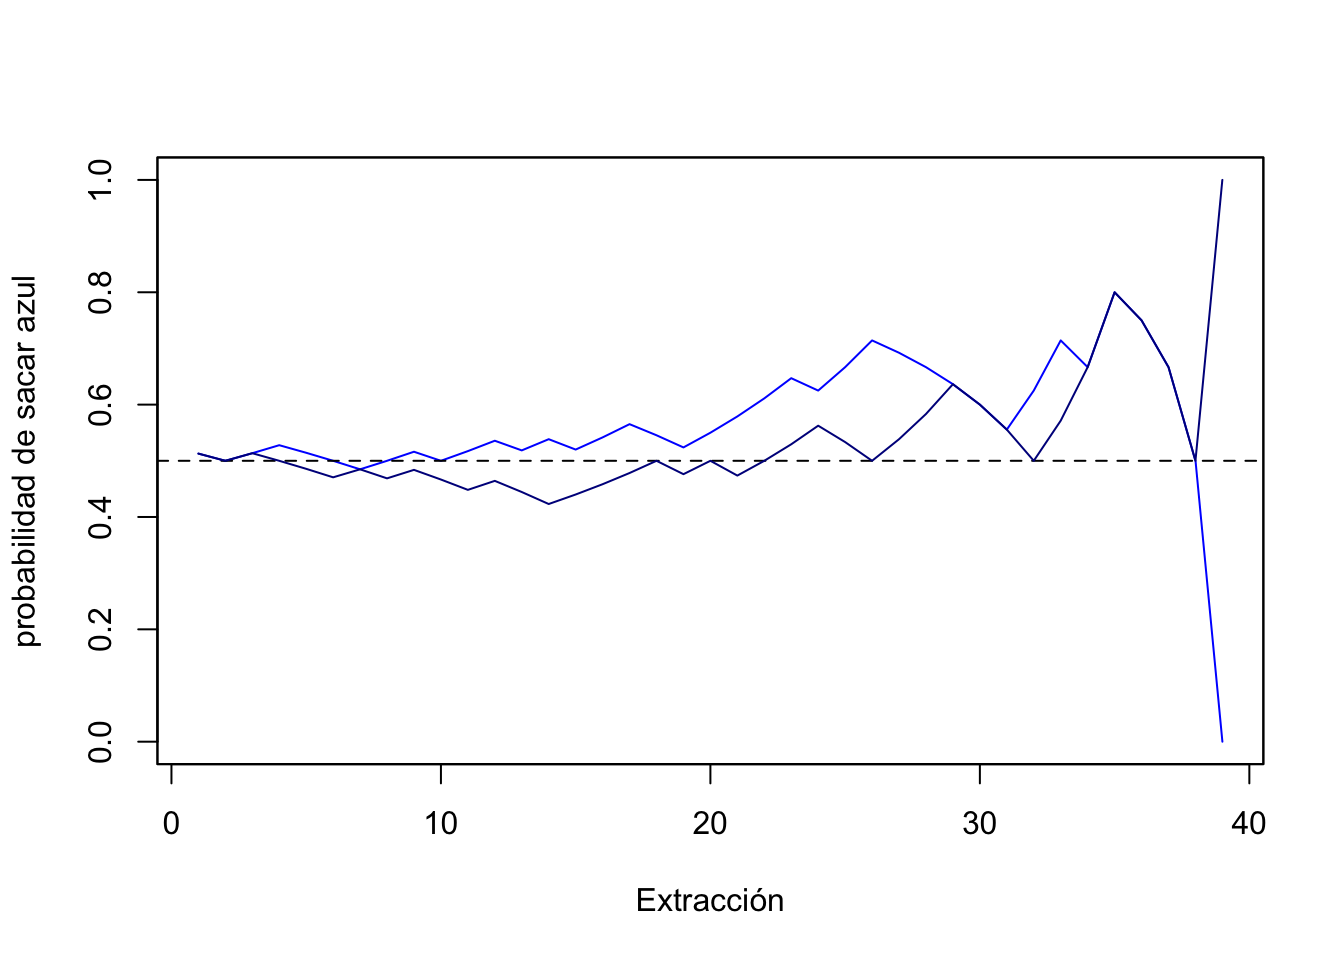
\includegraphics[width=0.8\linewidth]{ApuntesGeneticaII_files/figure-latex/figura3p2-1} 

}

\caption{Probabilidad de sacar una bolita azul en la próxima extracción, para un nuevo experimento (en rojo), con las mismas condiciones iniciales.}\label{fig:figura3p2}
\end{figure}

Claramente, el inicio del experimento es igual al del anterior (en los dos partimos de \(p_{azul}=\frac{1}{2}\)), y el mismo debe terminar en una proporción de bolitas azules de 0 o de 1, cuando no queden más bolitas azules o cuando todas las que queden sean azules (esa es la razón también por la que no ploteamos hasta después de la última extracción).

¿Qué ocurriría con nuestro experimento si hubiésemos tomado otro punto de partida (\emph{i.e.}, distinto número de bolitas azules que rojas), o si hubiésemos arrancado desde un número mayor o menor de bolitas?. Afortunadamente, es muy fácil realizar estos experimentos en una computadora y analizar los resultados, al menos para tener una primera impresión del comportamiento cualitativo del sistema. En la Figura \ref{fig:figura3p3} se observa qué ocurre al variar el número de bolitas en nuestra jarra (columna de la izquierda: 20 bolitas, columna de la derecha: 120 bolitas) y variando la frecuencia (proporción) de bolitas azules al comienzo (fila superior: \(p_{azul}=\frac{1}{2}\), fila inferior: \(p_{azul}=\frac{3}{4}\)).

\begin{figure}[H]

{\centering 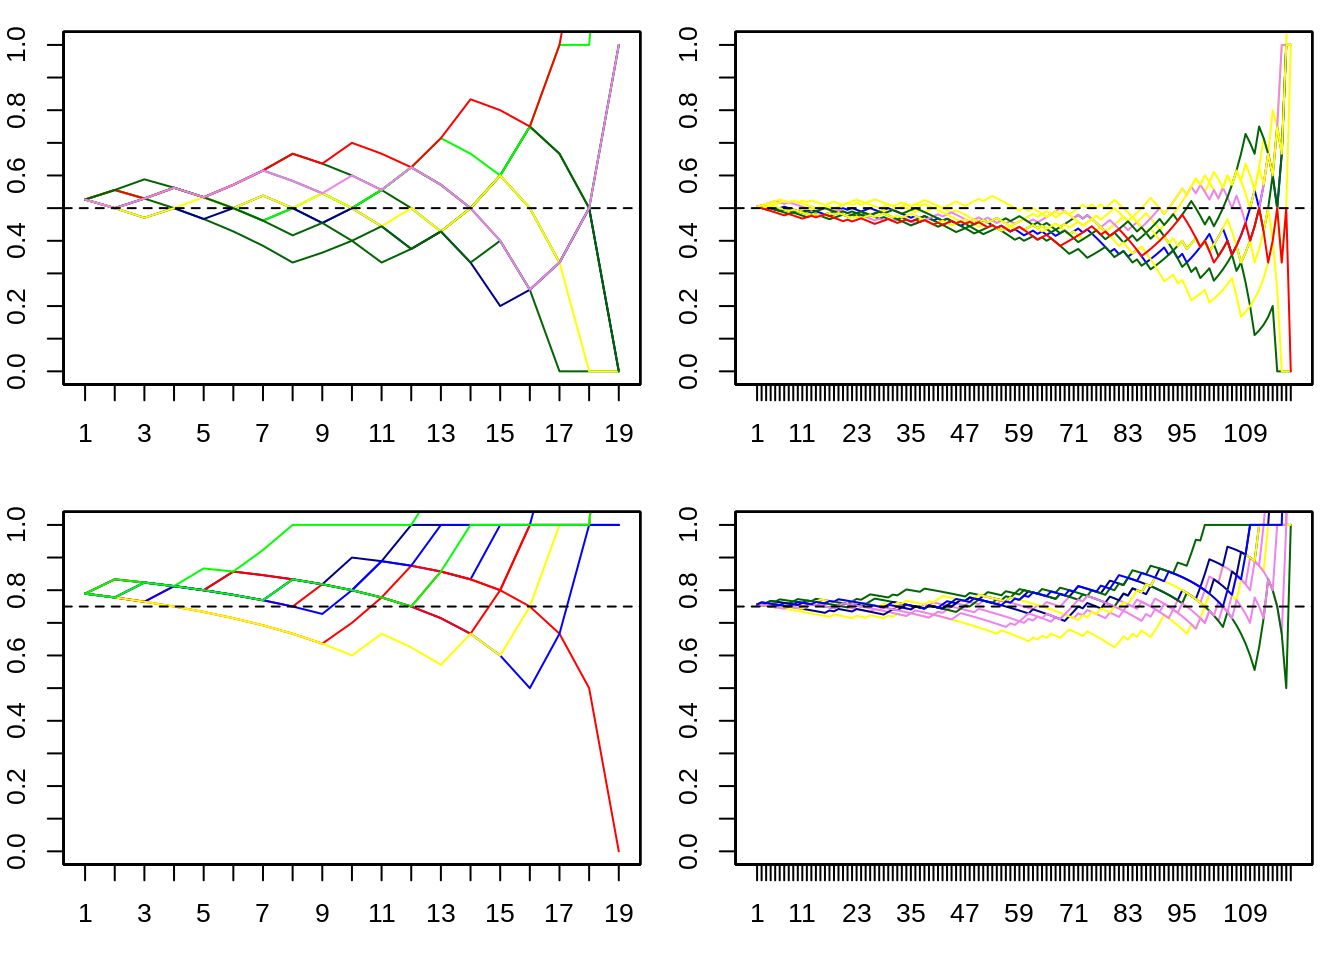
\includegraphics[width=0.8\linewidth]{ApuntesGeneticaII_files/figure-latex/figura3p3-1} 

}

\caption{Probabilidad de sacar una bolita azul en la próxima extracción, para 10 experimentos, para 4 condiciones: p=1/2 (arriba) y p=3/4 abajo, en 20 (izquierda) y 120 (derecha) bolitas.}\label{fig:figura3p3}
\end{figure}

A partir de la Figura \ref{fig:figura3p3} podemos empezar a sacar algunas conclusiones de este experimento aleatorio que nos servirán de referencia en breve. La primera conclusión se relaciona con algo que ya habíamos visto: \textbf{a medida que quedan menos bolitas en la jarra, ya sea porque se comenzó con pocas o porque el experimento se acerca a su fin, las variaciones en frecuencias suelen ser más drásticas}. Esto se puede observar, por ejemplo, en la figura de arriba a la derecha: al principio las variaciones entre distintas réplicas del experimento apenas se apartan de la línea a trazos, pero a medida que quedan menos bolitas (aumenta el número de experimentos que ya realizamos) las proporciones en cada experimento empiezan a ser cada vez más variables (existe mayor dispersión en torno a la línea a trazos). La segunda conclusión refiere al punto de partida del experimento: \textbf{a medida de que nos alejamos del punto medio (igual proporción de bolitas azules que rojas), mayor es la probabilidad de que la última bolita que quede en la jarra sea una bolita del tipo con mayor proporción inicial}. De hecho, la probabilidad de que la última bolita sea de uno de los dos colores, si realizamos repetidas veces el mismo experimento, es la probabilidad inicial del tipo al que pertenece dicha bolita. Podemos ver esto claramente a partir de un ejemplo. Supongamos que tenemos al inicio 10 bolitas en la jarra, 9 de ellas azules y una roja. Para que la roja sea la última en salir, todas las anteriores extracciones deben dar como resultado bolitas azules. La probabilidad de que la bolita roja sobreviva a la primer extracción (o sea, que la primer bolita sea azul) es \(\frac{9}{10}\) (ya que hay 9 bolitas azules y solo una roja). La de la segunda, asumiendo que la primera fue azul y que por lo tanto la bolita roja sobrevivió a la primer tirada, es de \(\frac{8}{9}\). La de la tercera será entonces \(\frac{7}{8}\), y así sucesivamente hasta que queden dos bolitas: una roja y otra azul. En este caso, la probabilidad de elegir nuevamente una bolita azul es de \(\frac{1}{2}\). Considerando estos eventos en conjunto (multiplicando sus respectivas probabilidades), tenemos:

\begin{equation}
P(\text{última}=\text{roja})=\frac{9}{10} \cdot \frac{8}{9} \cdot \frac{7}{8} \cdot ...  \cdot \frac{1}{2}=\frac{\prod_{1}^9}{\prod_{2}^{10}}=\frac{9!}{10!}=\frac{1}{10}
\end{equation}

que es la proporción de bolitas rojas al inicio \footnote{Recordemos que \(\prod_a^b\) simboliza a la productoria de \(a\) a \(b\). Esta operación es análoga a la sumatoria, pero en lugar de calcularse la suma de los números entre \(a\) y \(b\), se considera el producto de estos números. A modo de ejemplo, \(\prod_1^5 = 1 \cdot 2 \cdot 3 \cdot 4 \cdot 5\).}.

De hecho, podemos generalizar fácilmente el razonamiento anterior a otra proporción de bolitas rojas y azules. Supongamos ahora que tenemos como punto de partida 4 bolitas rojas y 6 azules. ¿Cuál es la probabilidad de que la última bolita sea de color rojo? Llamemos \(n\) al número total de bolitas (\(n=10\), en nuestro experimento) y \(k\) al número de bolitas rojas (\(k=4\), ídem). El total de posibles órdenes en que salen \textbf{todas} las bolitas es igual a las permutaciones de \(n\) elementos, dado por \(\mathbb{P}(n)=n!\). Para que la ultima bolita sea roja, separamos una de ellas del conjunto, por lo que ahora solo tenemos \(n-1=9\) bolitas. Notemos que el orden de salia de las mismas es irrelevante, por lo que hay \(\mathbb{P}{(n-1)}=(n-1)!\) posibilidades (órdenes de salida) de que esto suceda. Por lo tanto, \textbf{dado que agarramos una bolita roja en particular}, la probabilidad de que esa salga última será \(\frac{\mathbb{P}{(n-1)}}{\mathbb{P}{(n)}}=\frac{(n-1)!}{n!}=\frac{\prod_{1}^{n-1}}{\prod_{1}^{n}}=\frac{1}{n}\). Sin embargo, hay \(k\) bolitas rojas \textbf{diferentes} y para cualquiera de ellas este razonamiento es válido, por lo que debemos multiplicar la probabilidad anterior por \(k\) (todos son eventos disjuntos). Considerando esto, tenemos que la probabilidad de que la última bolita sea roja es

\begin{equation}
\mathbb{P}(\text{última}=\text{roja})=k \frac{\mathbb{P}{(n-1)}}{\mathbb{P}{(n)}}=k \frac{(n-1)!}{n!}=k \frac{\prod_{1}^{n-1}}{\prod_{1}^{n}}=\frac{k}{n}
\end{equation}

que es la probabilidad inicial de sacar una bolita roja (\(k/n\), \(4/10\) en nuestro caso) o, lo que es lo mismo, la proporción inicial de bolitas rojas. La utilidad de todo este razonamiento lo veremos en la siguiente sección (\hyperref[el-modelo-de-wright-fisher]{El modelo de Wright-Fisher}
).

\begin{graybox}

\begin{itemize}
\tightlist
\item
  La importancia de las \textbf{proporciones de partida} puesto que estas determinaran las probabilidades de obtener cierto resultado.
\item
  Las \textbf{barreras absorbentes} serán aquellos valores que no podremos sobrepasar, y representarán los ``límites'' de los que no podremos escapar hacia otros valores.
\end{itemize}

\end{graybox}

\section{El modelo de Wright-Fisher}\label{el-modelo-de-wright-fisher}

A esta altura, ya habrás comenzado a imaginarte la relación entre los experimentos aleatorios de la sección anterior y nuestro modelo de poblaciones con un número relativamente pequeño de individuos. Si bien es posible imaginarse y modelar todo el proceso de gametogénesis, apareamientos al azar para constituir los genotipos de la próxima generación y repetir esto tantas veces como queramos, Sewall Wright \footnote{Sewall Green Wright (21 de diciembre, 1889 - 3 marzo, 1988), fue
  un genetista que realizó notables aportes sobre los efectos de la
  selección y la deriva, así como el análisis de pequeñas poblaciones
  y el efecto de la consanguinidad . Junto a Ronald A. Fisher y JBS
  Haldane establecieron la fundación matemática de la genética de
  poblaciones y de la teoría evolutiva.} y Ronald Fisher \footnote{Sir Ronald Aylmer Fisher (17 de febrero 1890 - 29 de julio 1962) fue un matemático, estadístico y biológo evolutivo inglés. A partir de los datos colectados en la Estación Experimental de Rothamsted desarrollo las bases estadísticas para el diseño de experimentos, desarrollo también el análisis de varianza y fue unos de los tres pioneros (junto a Sewall Wright y John Burdon Sanderson Haldane) que participaron de la fundación de la teoría en genética de poblaciones, el neo-darwinismo y la síntesis moderna de la evolución.} imaginaron un procedimiento mucho más sencillo que permite arribar a las misma conclusiones con mucho menos esfuerzo de cálculo.

La primera suposición que hace el modelo de Wright-Fisher es que, más allá del número de individuos, el \textbf{pool de gametos} (el conjunto de todos los gametos en la población) es infinito. Si bien esto puede parecer extraño, es importante recordar que el número de espermatozoides (gametos masculinos) que producen los machos es virtualmente enorme, y el número de óvulos que produce cada hembra es de órdenes de magnitud superior que su descendencia; teniendo esto en cuenta, este no parece un supuesto arriesgado. Los otros supuestos incluyen: \emph{i)} ausencia de selección, \emph{ii)} ausencia de mutaciones, \emph{iii)} ausencia de migración, \emph{iv)} tiempos de generación no superpuestos, y \emph{v)} apareamiento aleatorio (panmixia). Si bien no suena realista que se cumplan todas estas condiciones en la vida real, el apartamiento de las mismas suele ser lo suficientemente menor como para considerar el modelo como una buena aproximación inicial. El proceso que plantean Wright-Fisher para el modelo de un gen con dos alelos es el siguiente: para una población de \(N\) individuos de una especie diploide, dada la frecuencia de uno de los alelos muestrear al azar del \textbf{pool infinito} \(2N\) alelos. Está será nuestra nueva población. La lógica del modelo Wright-Fisher se ve graficada para un caso con \(N\) individuos en la Figura \ref{fig:jarra-fisher-wright}, donde además se hace explícita la analogía con el experimento mental de bolitas que desarrollamos anteriormente.

\begin{figure}[H]

{\centering 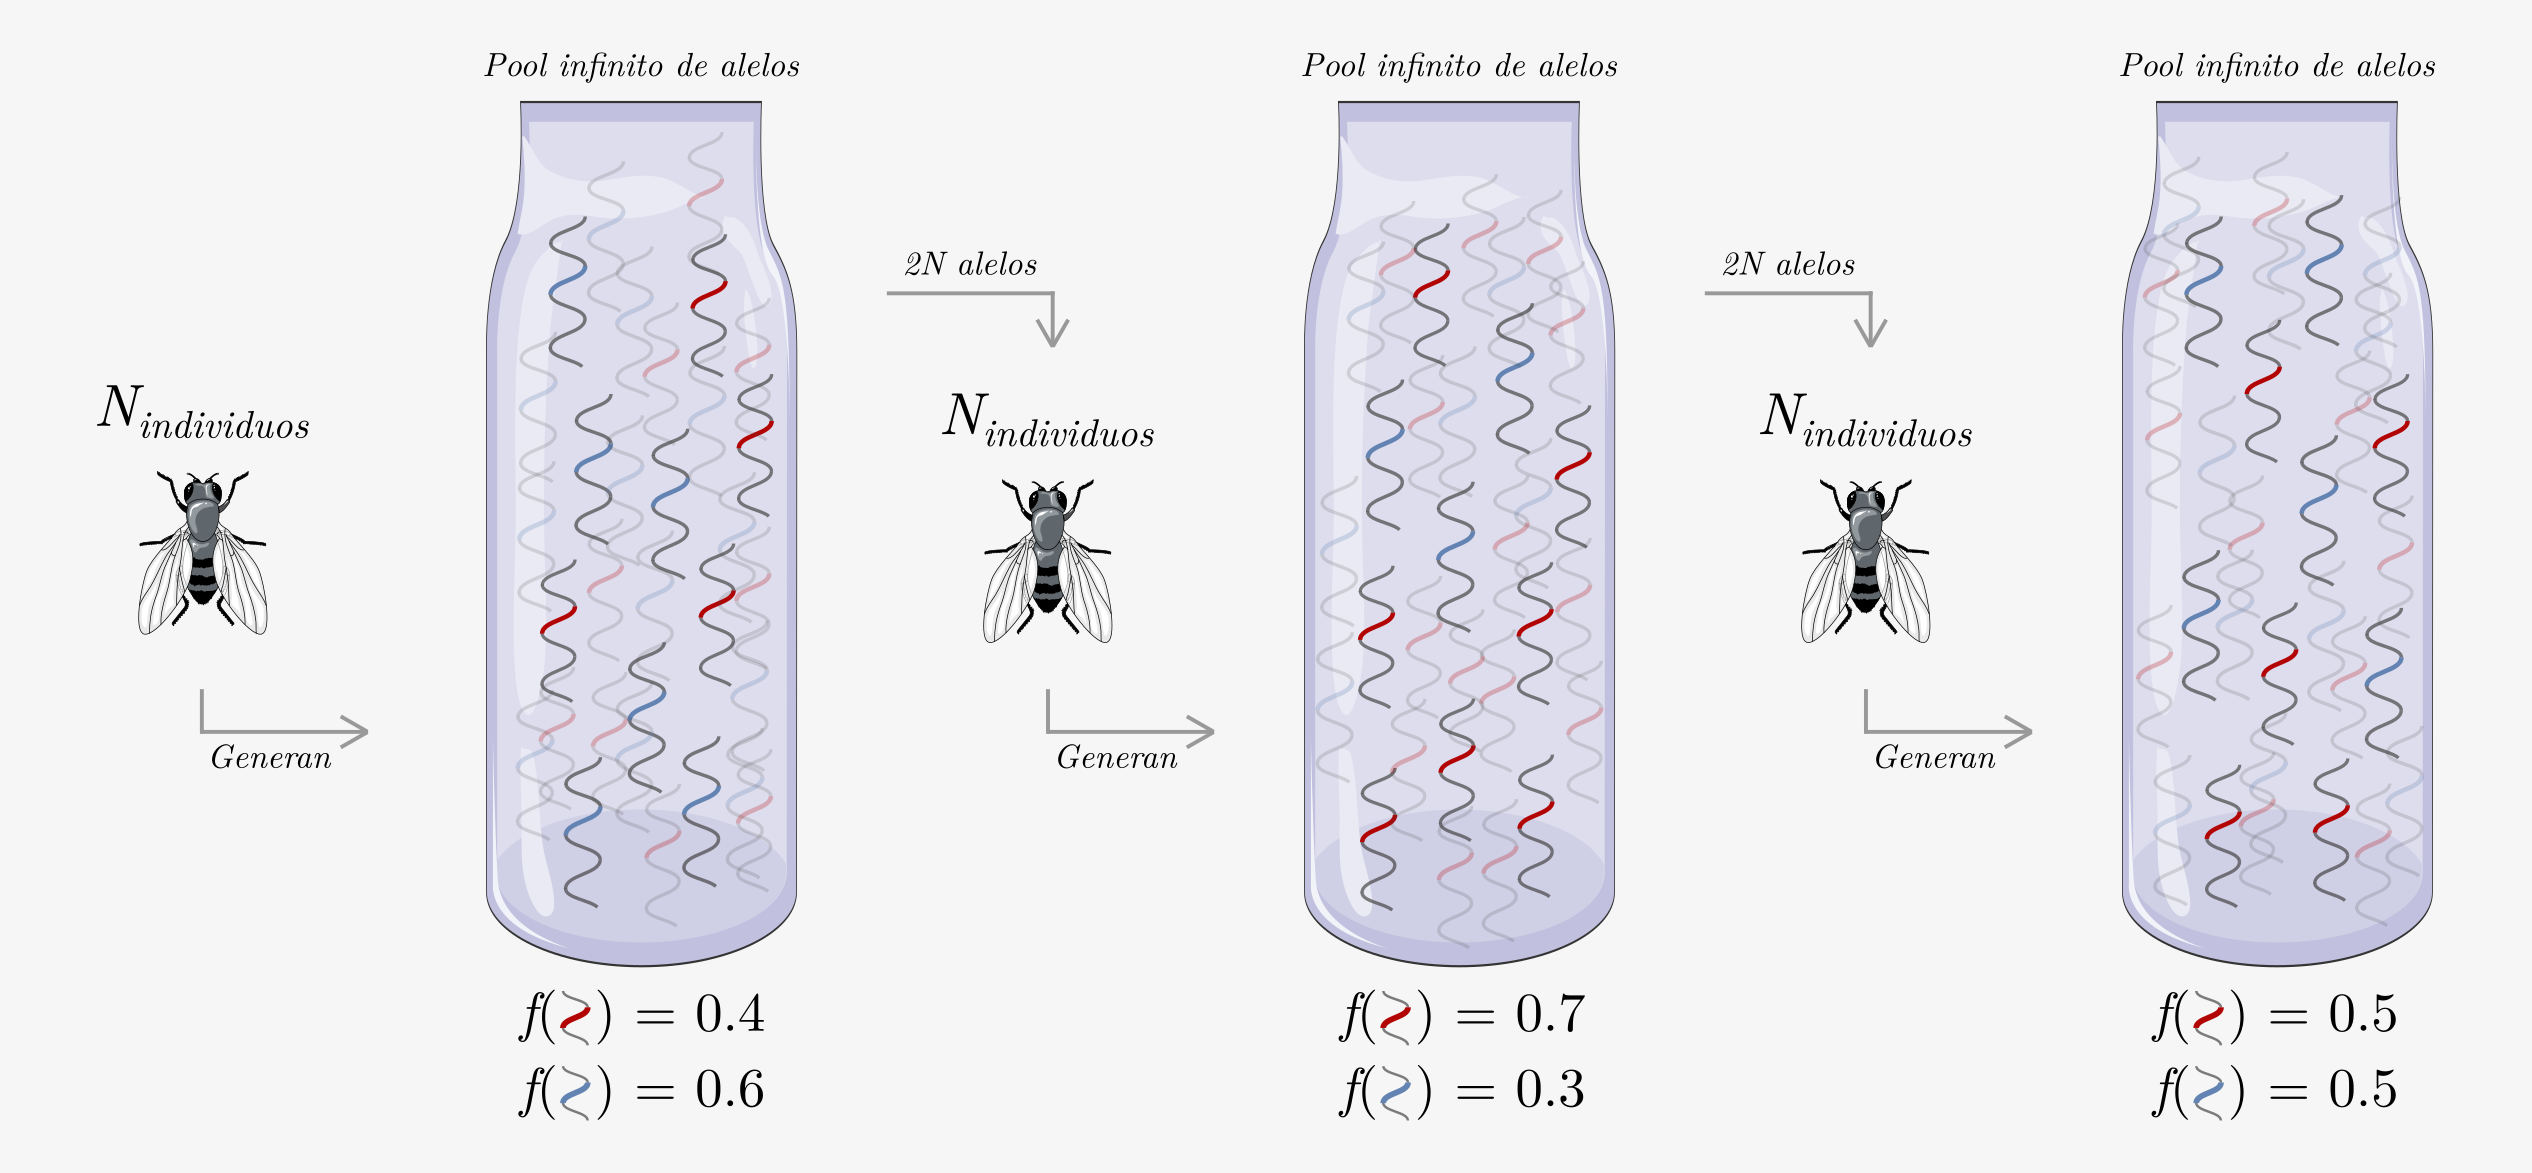
\includegraphics[width=1\linewidth]{figuras/jarra-fisher-wright} 

}

\caption{Representación esquemática del modelo de Wright-Fisher. Una población finita de N individuos (de la especie \textit{D. melanogaster}, en este ejemplo) generan en cada generación un pool infinito de alelos que mantiene las frecuencias alélicas de la generación. La próxima generación se compone muestreando 2N alelos con reposición, los cuales conformarán a los N individuos de la generación. Imagen creada con elementos gráficos tomados de bioicons (https://bioicons.com/).}\label{fig:jarra-fisher-wright}
\end{figure}

Podemos repetir el procedimiento. tantas veces como queramos para estudiar el comportamiento a lo largo del tiempo de nuestro modelo. hora, suponemos que ya te habrás preguntado cómo hacemos para muestrear de un pool infinito a partir de un número limitado de alelos disponibles (\(2N\)). El truco es muy sencillo, la diferencia entre un muestreo \textbf{con reposición} y un muestreo \textbf{sin reposición} (el que hicimos en la sección precedente) es que mientras que en este último las frecuencias van variando a medida de que vamos extrayendo muestras, en el primero (\textbf{con reposición}) las frecuencias permanecen incambiadas definitivamente. Claramente, cuando el muestreo es de a una bolita (o alelo) esto se asemeja a muestrear de un pool infinito de bolitas (o alelos).

Veamos cómo funciona en la práctica. Supongamos que tenemos una población de \(N=5\) individuos. Supongamos además de que se trata de un \emph{locus} con dos alelos, \(A\) representado por bolitas azules y \(a\) representado por las bolitas rojas. Para simplificar y que se fije la idea del procedimiento vamos a comenzar con una frecuencia inicial de \(p_A=p_{azul}=\frac{1}{2}=p_{roja}=p_a\). Para que nuestro procedimento funcione claramente vamos a tener ahora dos jarras (una inicialmente con igual proporción de bolitas azules y rojas y la otra vacía) y una caja con al menos \(2N\) bolitas de cada color, o sea que en nuestro ejemplo, al menos 10 bolitas azules y 10 bolitas rojas.

La jarra vacía va a representar una nueva generación de nuestra población. Para completarla procederemos extrayendo al azar de la \textbf{jarra llena} una bolita y de acuerdo al color de la misma sacamos \textbf{de la caja} una bolita del mismo color y la colocamos en la \textbf{jarra vacía}, devolviendo la bolita que sacamos a la jarra llena. Repetimos este procedimiento \(2N\) veces, al cabo del cual tendremos \(2N\) bolitas en nuestra antigua \textbf{jarra vacía} (la nueva generación de la población). Para completar el procedimiento y estar prontos para una nueva generación, vaciamos el contenido de la anterior \textbf{jarra llena} en la caja.

En este punto, podemos analizar el contenido de la \textbf{nueva jarra llena} (la población ``hija'' de la inicial), contando cuántas bolitas de cada color obtuvimos. Ahora, ¿podemos predecir (de alguna manera) el comportamiento de este experimento en una generación? Si llamamos (arbitrariamente) un ``éxito'' al hecho de sacar una bolita de color azul, entonces la extracción de cada bolita será una variable aleatoria con distribución de Bernoulli\footnote{Jacob Bernoulli (6 de enero 1655 - 16 de agosto 1705) fue un matemático Suizo que realizó diversos descubrimientos importante y uno de promotores tempranos del cálculo integral. Miembro de las academias reales de París y Berlín, la distribución lleva su nombre en homenaje a sus contribuciones.} y probabilidad de éxito \(p_{azul}\) (y por lo tanto, probabilidad de fracaso, bolita roja, \(p_{roja}=1-p\)). Si consideramos el resultado de las \(2N\) extracciones independientes y con la misma probabilidad (recordar que es un muestreo \textbf{con reposición}) como un conjunto, entonces la distribución del número de bolitas azules (éxitos) y rojas (fracasos) entre las \(2N\) tenga una distribución binomial:

\[
\begin{split}
P(i \text{ bolitas azules})={2N\choose i} p^i (1-p)^{2N-i},\\
{2N\choose i}=\frac{2N!}{i!(2N-i)!}
\end{split}
\label{eq:binomi2}
\]

Es decir, si bien el número de bolitas en la nueva jarra también es de \(2N=10\), ahora el número de bolitas azules (copias del alelo \textbf{A}) que llamamos \(i\) (y por lo tanto el de bolitas rojas, o alelo \textbf{a} igual a \(2N-i\)) es una variable aleatoria y por lo tanto con resultado incierto de experimento en experimento. En general, si una población tiene \(i\) copias del alelo \(A\) y \(2N-i\) copias del alelo \(a\), la probabilidad de transición de pasar de \(i\) copias a \(j\) copias en el modelo de Wright-Fisher se encuentra dada por la siguiente ecuación:

\begin{equation}
T_{ij}={2N \choose j}\left(\frac{i}{2N}\right)^{j}\left(\frac{2N-i}{2N}\right)^{2N-j}=\frac{(2N)!}{j!(2N-j)!}p^jq^{2N-j}
\label{eq:WrightFisher}
\end{equation}

Esta ecuación es bien sencilla de explicar. La probabilidad de éxito (alelo \textbf{A} o bolita azul) varía de generación en generación, y por lo tanto para la generación actual de gametos es igual a la proporción de alelos \textbf{A} (\(i\)) en el total (\(2N\)), por lo que para cada generación de gametos \(p=\frac{i}{2N}\). Concomitantemente, la probabilidad de fracaso (alelo \textbf{a} o bolita roja) es igual a la proporción de alelos \textbf{a} en el total, o sea \(\frac{2N-i}{2N}\). Ahora, al número de éxitos \textbf{en la siguiente generación} le llamamos \(j\) (la cantidad de alelos \textbf{A} que tienen la probabilidad \(T_{ij}\)) y por lo tanto, la cantidad de alelos \textbf{a} será \(2N-j\).

Hasta ahora nos hemos referido a una población en particular y como vimos su evolución es completamente al azar. En la Figura \ref{fig:figura3p4} podemos ver un ejemplo de la evolución del alelo \textbf{A} en una población de 5 individuos diploides. El punto de partida es de \(p_{A}=\frac{1}{2}\) y el aspecto de ``dientes de sierra'' se debe a que lo más fino que puede ser el movimiento es de \(\frac{1}{2N}=\frac{1}{10}=0,1\) en nuestro caso. Por otro lado, tanto \(p_A=0\) como \(p_A=1\) son \textbf{barreras absorbentes} ya que \(p_A=0\) quiere decir que no quedan más alelos \textbf{A} (bolitas azules) en la población, mientras que \(p_A=1\) quiere decir que todos los alelos que quedan en la población son \textbf{A}, es decir que este alelo se fijó en la población (y por lo tanto, en ambos casos la frecuencia no variará más en el tiempo; recordar que uno de los supuestos fue que no hay mutación).

Afortunadamente a partir de unas pocas líneas de código podemos explorar a nuestro antojo el comportamiento en varias poblaciones, conjunto que se llama \textbf{\emph{ensemble}} (del francés, el conjunto de todos los individuos de todas las poblaciones; ver Figura \ref{fig:ensemble}), variando el número de individuos en ellas, así como la proporción inicial del alelo \textbf{A}. El resultado de probar el comportamiento para poblaciones de 5 y 50 individuos, con proporción inicial de alelo de \(p=\frac{1}{2}\) y \(p=\frac{3}{4}\) lo podemos ver en la Figura \ref{fig:figura3p5}. Claramente podemos apreciar que las poblaciones con mayor número de individuos tienen un comportamiento menos errático. Por otro lado, en las poblaciones que arrancan más cerca de una de las \textbf{barreras absorbentes} la variación es menor en relación a las poblaciones con el mismo número de individuos que arrancan desde la mitad (\(p=\frac{1}{2}\)).

\begin{figure}[H]

{\centering 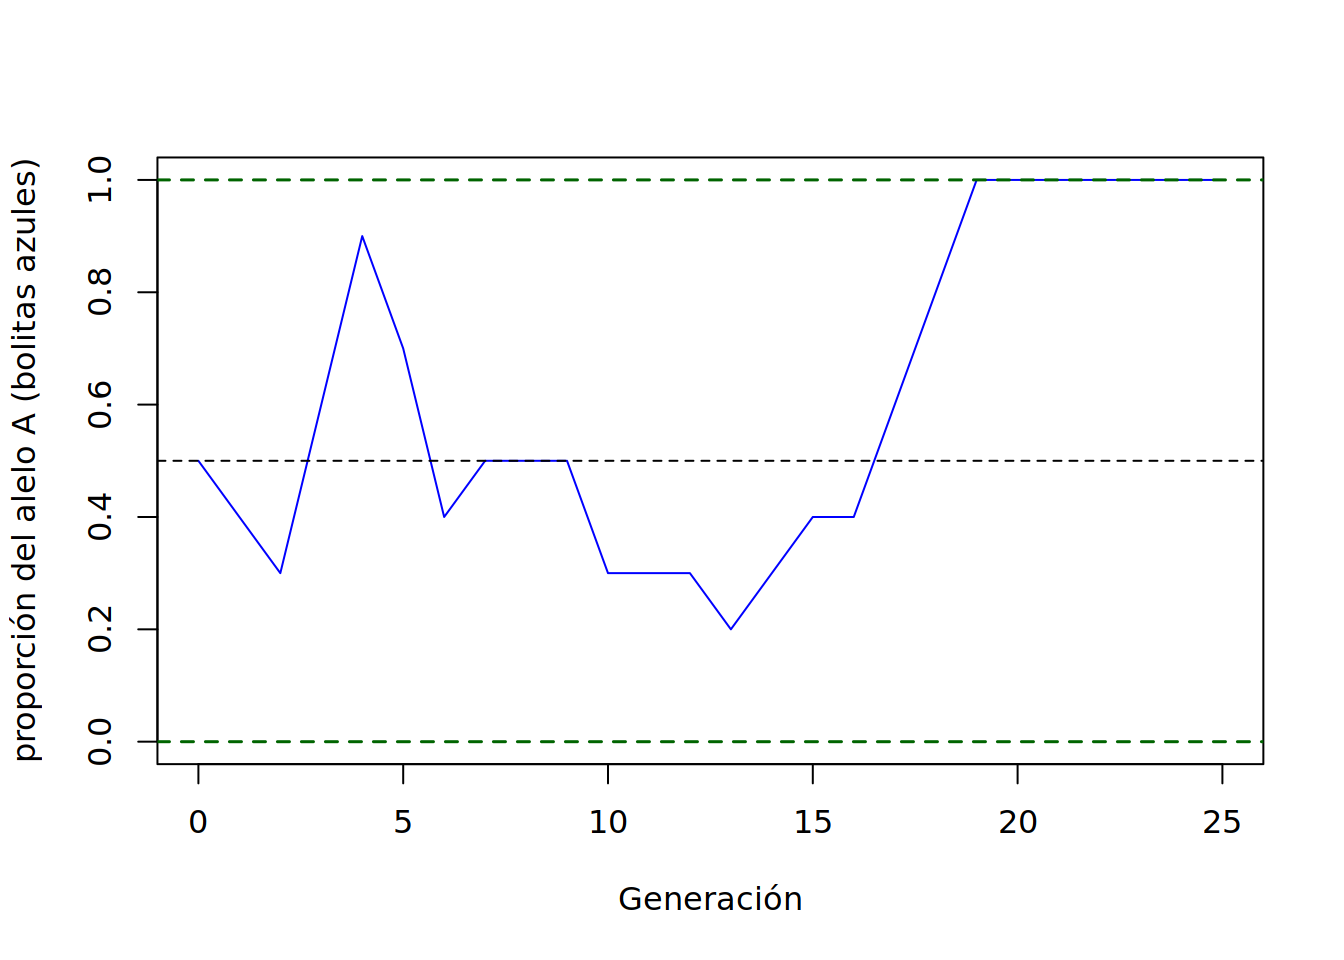
\includegraphics[width=0.62\linewidth]{ApuntesGeneticaII_files/figure-latex/figura3p4-1} 

}

\caption{Proporción del alelo A (bolitas azules) en una población de 5 individuos diploides. Notar de que se trata de una realización en particular de este experimento y que con seguridad si repetimos el experimento el resultado será diferente.}\label{fig:figura3p4}
\end{figure}

\begin{figure}[H]

{\centering 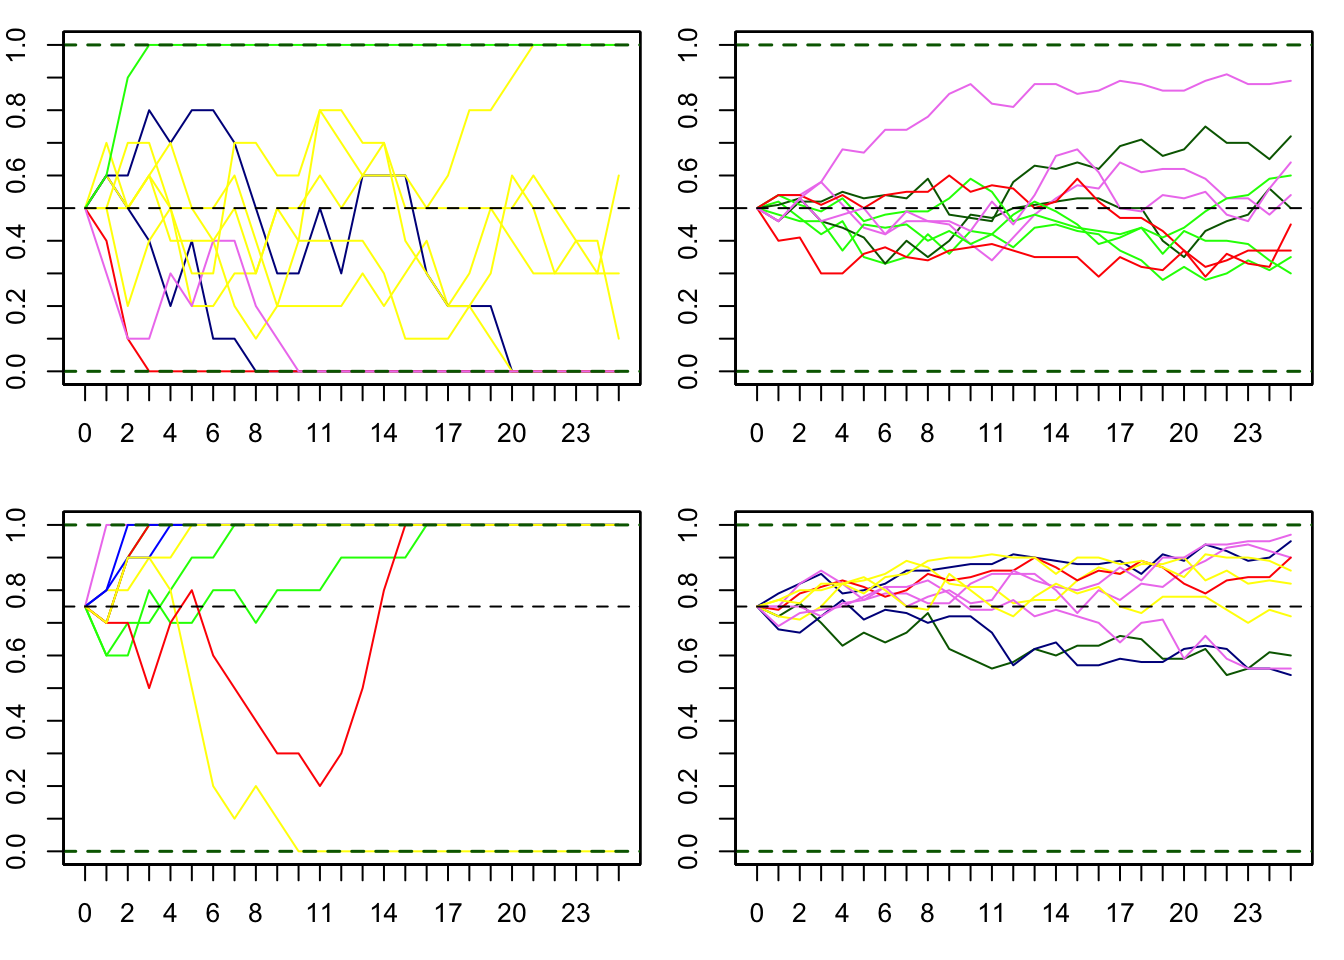
\includegraphics[width=0.72\linewidth]{ApuntesGeneticaII_files/figure-latex/figura3p5-1} 

}

\caption{Frecuencia del alelo A (bolitas azules) en 10 poblaciones de 5 individuos diploides (a la izquierda) y de 50 individuos diploides (derecha), para frecuencias iniciales de p=1/2 (arriba) y p=3/4 (abajo).}\label{fig:figura3p5}
\end{figure}

Este comportamiento no debería resultarnos extraño. Los muestreos que estamos realizando en cada población, a cada generación, provienen de distribuciones binomiales. Si recuerdas de tus cursos de matemáticas y estadística, para una variable \(i \sim Binom(2N,p)\) se tiene valor esperado \(E(i)=2Np\) y varianza \(\sigma^2(i)=2Np(1-p)=2Np-2Np^2\), por lo que esperamos que mientras las poblaciones se encuentren segregando, la esperanza (la media) entre la distintas poblaciones sea de \(Np\), o lo que es lo mismo, la proporción del alelo \textbf{A} sea igual a \(p_A=\frac{E(i)}{2N}=\frac{2Np}{2N}=p\) (es decir, en promedio las líneas de poblaciones oscilarán en torno a la frecuencia inicial). Más aún, como vimos antes (\hyperref[heterocigotas-freq-alelica]{H-W: la frecuencia de heterocigotas en función de la frecuencia alélica}), \(p(1-p)\) tiene un máximo en \(p=\frac{1}{2}\), por lo que la varianza \(\sigma^2(i)=2Np(1-p)\) también tendrá un máximo en \(p=\frac{1}{2}\) (porque \(p(1-p)\) está multiplicado por \(2N\) que es necesariamente una constante positiva); en otras palabras, la varianza \textbf{dentro de cada población} será máxima cerca de la frecuencia \(p=\frac{1}{2}\).
¿Cómo se condice esto con el comportamiento más variable en poblaciones pequeñas? Si recuerdas de esos mismos cursos, la varianza en la frecuencia por \textbf{generación} en el \textbf{\emph{ensemble}} viene dada por

\begin{equation}
\sigma^2(i/(2N_e))= \frac{1}{(2N_e)^2} \cdot \sigma^2(i) 
\sigma^2(p)=\frac{2 N_e p(1-p)}{4 N_e^2}=\frac{p(1-p)}{2N_e} \Rightarrow 
\end{equation}

\begin{equationbox}
\begin{equation}
\sigma^2(p)=\frac{pq}{2N_e}=\frac{p-p^2}{2N_e}
\end{equation}

\end{equationbox}

Es decir que al aumentar el tamaño de cada población (\(2N\)) la variación \textbf{entre poblaciones} disminuye. Finalmente, la variación \textbf{entre poblaciones} para las poblaciones que aún se encuentran segregando (o sea, que no llegaron a las \textbf{barreras absorbentes}) se incrementa con el tiempo de manera aproximadamente lineal, por lo que para tiempo \(t\) en las líneas que continúan segregando esperamos una varianza de

\begin{equationbox}
\begin{equation}
\sigma_t^2(p)=t\frac{pq}{2N}=t\frac{(p-p^2)}{2N}.
\end{equation}

\end{equationbox}

Una última observación es la que hace al número de individuos \(N\) de las distintas poblaciones. Hasta ahora asumimos que cada uno de nuestros individuos era completamente independiente de los otros desde el punto de vista genético (es decir, asumimos condiciones ideales) y por lo tanto no tuvimos en cuenta el efecto de que se puedan ver emparentadas en nuestros cálculos. En realidad, en la práctica, bajo diferentes criterios (apareamientos dirigidos, diferencias en el número de progenie esperada por pareja, etc.), las poblaciones se suelen comportar como si el número de individuos fuese menor y a ese número se lo conoce como \textbf{tamaño efectivo} de la población y se lo representa con el símbolo \(N_e\). Esto lo veremos con más detalle en la sección \hyperref[tamauxf1o-efectivo-poblacional]{Tamaño efectivo poblacional} y de nuevo en el capítulo \hyperref[aparnoalazar]{Apareamientos no-aleatorios}.

En resumen, a partir del modelo sencillo de Wright-Fisher pudimos entender que \textbf{en ausencia de otras fuerzas evolutivas como la selección, migración o mutación, las frecuencias alélicas pueden variar en forma aleatoria y que con el transcurso del tiempo cada alelo puede fijarse en alguna población mientras que desaparece en otras}. Este fenómeno es lo que se conoce como \textbf{deriva genética} o \textbf{deriva aleatoria}, este último término en razón de que el cambio en las frecuencias no tiene una dirección y que por lo tanto no es predecible el sentido para una población en particular.

\subsection*{Ejemplo 3.1}\label{ejemplo-3.1}
\addcontentsline{toc}{subsection}{Ejemplo 3.1}

Una población de 1000 individuos es dividida en cuatro subpoblaciones, cada una con un tamaño poblacional efectivo de 250 individuos.
Las poblaciones se encuentran segregando un locus bi-alélico, siguiendo todos los supuestos esperados para encontrarse en equilibrio de Hardy-Weinberg (salvo el de tamaño poblacional infinito).
Luego de un tiempo, se observan las siguientes frecuencias alélicas (\(p_i\)) para el alelo \(A_1\) en el \emph{ensemble} de subpoblaciones: \(p_1 = 0,39;\ p_2 = 0,61 ;\ p_3 = 0,57;\ p_4 = 0,42\).
Estime el número de generaciones transcurrido desde la formación del \emph{ensemble} de subpoblaciones.

A partir de las frecuencias alélicas observadas en el \emph{ensemble} se estima una frecuencia promedio \(\bar{p} = \frac{0.39+0.61+0.57+0.42}{4} = 0.4975\).
A su vez, la varianza observada para la frecuencia alélica en el ensemble es de \(\sigma_t^2(p) = \frac{1}{n}\sum_{i=1}^{i=n}(p_i - \bar{p})^2 = \frac{(0.39-0.4975)^2 + (0.61-0.4975)^2 + (0.57-0.4975)^2 + (0.42-0.4975)^2}{4} \Rightarrow \sigma_t^2(p) = 0, 00886875\).

Dado que la varianza para la frecuencia alélica \(p\) aumenta linealmente con el tiempo generacional \(t\) según la ecuación \(\sigma^2_t(p) = t \cdot \frac{pq}{2N_e}\), podemos usar nuestro estimado de \(\bar{p}\) y el tamaño poblacional efectivo \(N_e = 250\) para calcular el número de generaciones transcurrido desde la generación del \emph{ensemble}:

\[\sigma^2_t(p) = t \cdot \frac{pq}{2N_e} \Rightarrow t = \frac{\sigma^2_t(p) \cdot 2N_e}{\bar{p}\bar{q}}\]

\[ t = \frac{0,00886875 \cdot 2\cdot250}{0,4975 \cdot (1-0,4975)}\]

por lo que inferimos que se estima pasaron \(t \approx 18\) generaciones desde la formación del \emph{ensemble} poblacional.

\begin{graybox}

\begin{itemize}
\tightlist
\item
  El modelo de \textbf{Wright-Fisher} asume que de un \textbf{pool infinito} de gametos, con las frecuencias de los alelos proporcionales a lo muestreado para constituir la generación anterior, muestreamos nuevamente \(2N\) alelos, que constituirá a la nueva población.
\item
  La suposición de un \textbf{pool infinito} de gametos es equivalente, desde el punto de vista matemático a un muestreo con reposición.
\item
  Al generarse la nueva población a partir de \(2N\) muestreos independientes de Bernoulli, la distribución de la nueva población será una Binomial con probabilidad \(p\) y tamaño \(2N\).
\item
  La varianza de las frecuencias del alelo \textbf{A} (\(p\)) entre poblaciones, \textbf{por generación}, debida al efecto de la deriva genética es:
\end{itemize}

\begin{equation*}
\sigma^2(p)=\frac{pq}{2N_e}=\frac{p-p^2}{2N_e}
\label{eq:varWFpergen}
\end{equation*}

siendo \(p\) y \(q\) (con \(q=1-p\)) las frecuencias de los alelos y \(N_e\) el tamaño efectivo de las poblaciones que forman el \textbf{ensemble}. Como la varianza crece linealmente con el tiempo (en generaciones), tenemos también que para el tiempo \(t\) para las líneas que continúan segregando:

\begin{equation*}
\sigma_t^2(p)=t\frac{pq}{2N_e}=t\frac{(p-p^2)}{2N_e}
\label{eq:varWF}
\end{equation*}

\end{graybox}

\section{La subdivisión poblacional y la evolución de las frecuencias alélicas}\label{la-subdivisiuxf3n-poblacional-y-la-evoluciuxf3n-de-las-frecuencias-aluxe9licas}

La sección anterior marcó un cambio importante en nuestras perspectivas. Desde analizar el comportamiento de una o dos poblaciones, a partir de la sección anterior empezamos a apreciar que el azar puede jugar un rol muy importante en la evolución de las frecuencias alélicas en poblaciones relativamente pequeñas y nos empezamos a interesar en la visión en conjunto de las mismas.

El debate acerca del rol de la deriva genética versus la selección en los procesos de especiación (la aparición de nuevas especies) ha sido acalorado (ver, por ejemplo B. Charlesworth, Lande, and Slatkin (\citeproc{ref-CharlesworthLandeSlatkin1982}{1982})). Aunque el debate continúa, pese a reconocer un rol no despreciable a la deriva genética, los actores principales de esta comedia que es la vida parecen ser la mutación (como generador de variabilidad) y la selección, a través de sus diversas formas de acción (algo que veremos en el capítulo de \hyperref[seleccion]{Selección Natural}).

Pero veamos cómo podría estar funcionando la deriva genética en los procesos que llevan a la especiación. En efecto, imaginemos un \emph{locus} con dos alelos que sean neutros respecto a los ambientes (por lo tanto no hay selección). Asumamos también que la tasa mutacional es suficientemente baja como para que resulte improbable la aparición de los mismos alelos. Supongamos también que se trata de una especie con poca movilidad esperada, o sea la relación entre su área potencial de apareamiento y el rango geográfico de la especie (pueden ser especies animales, plantas, hongos, por ejemplo). Si la dispersión a largas distancias en esta especie suele ser algo relativamente raro, por ejemplo semillas llevadas por el viento, es posible imaginar que el \textbf{ensemble} de poblaciones está formado por pequeños \textbf{parches}, cada uno constituyendo una población diferente y que dada la baja movilidad de la especie no es probable que intercambien material genético con otros parches (ver representación en la Figura \ref{fig:ensemble}).

\begin{figure}[H]

{\centering 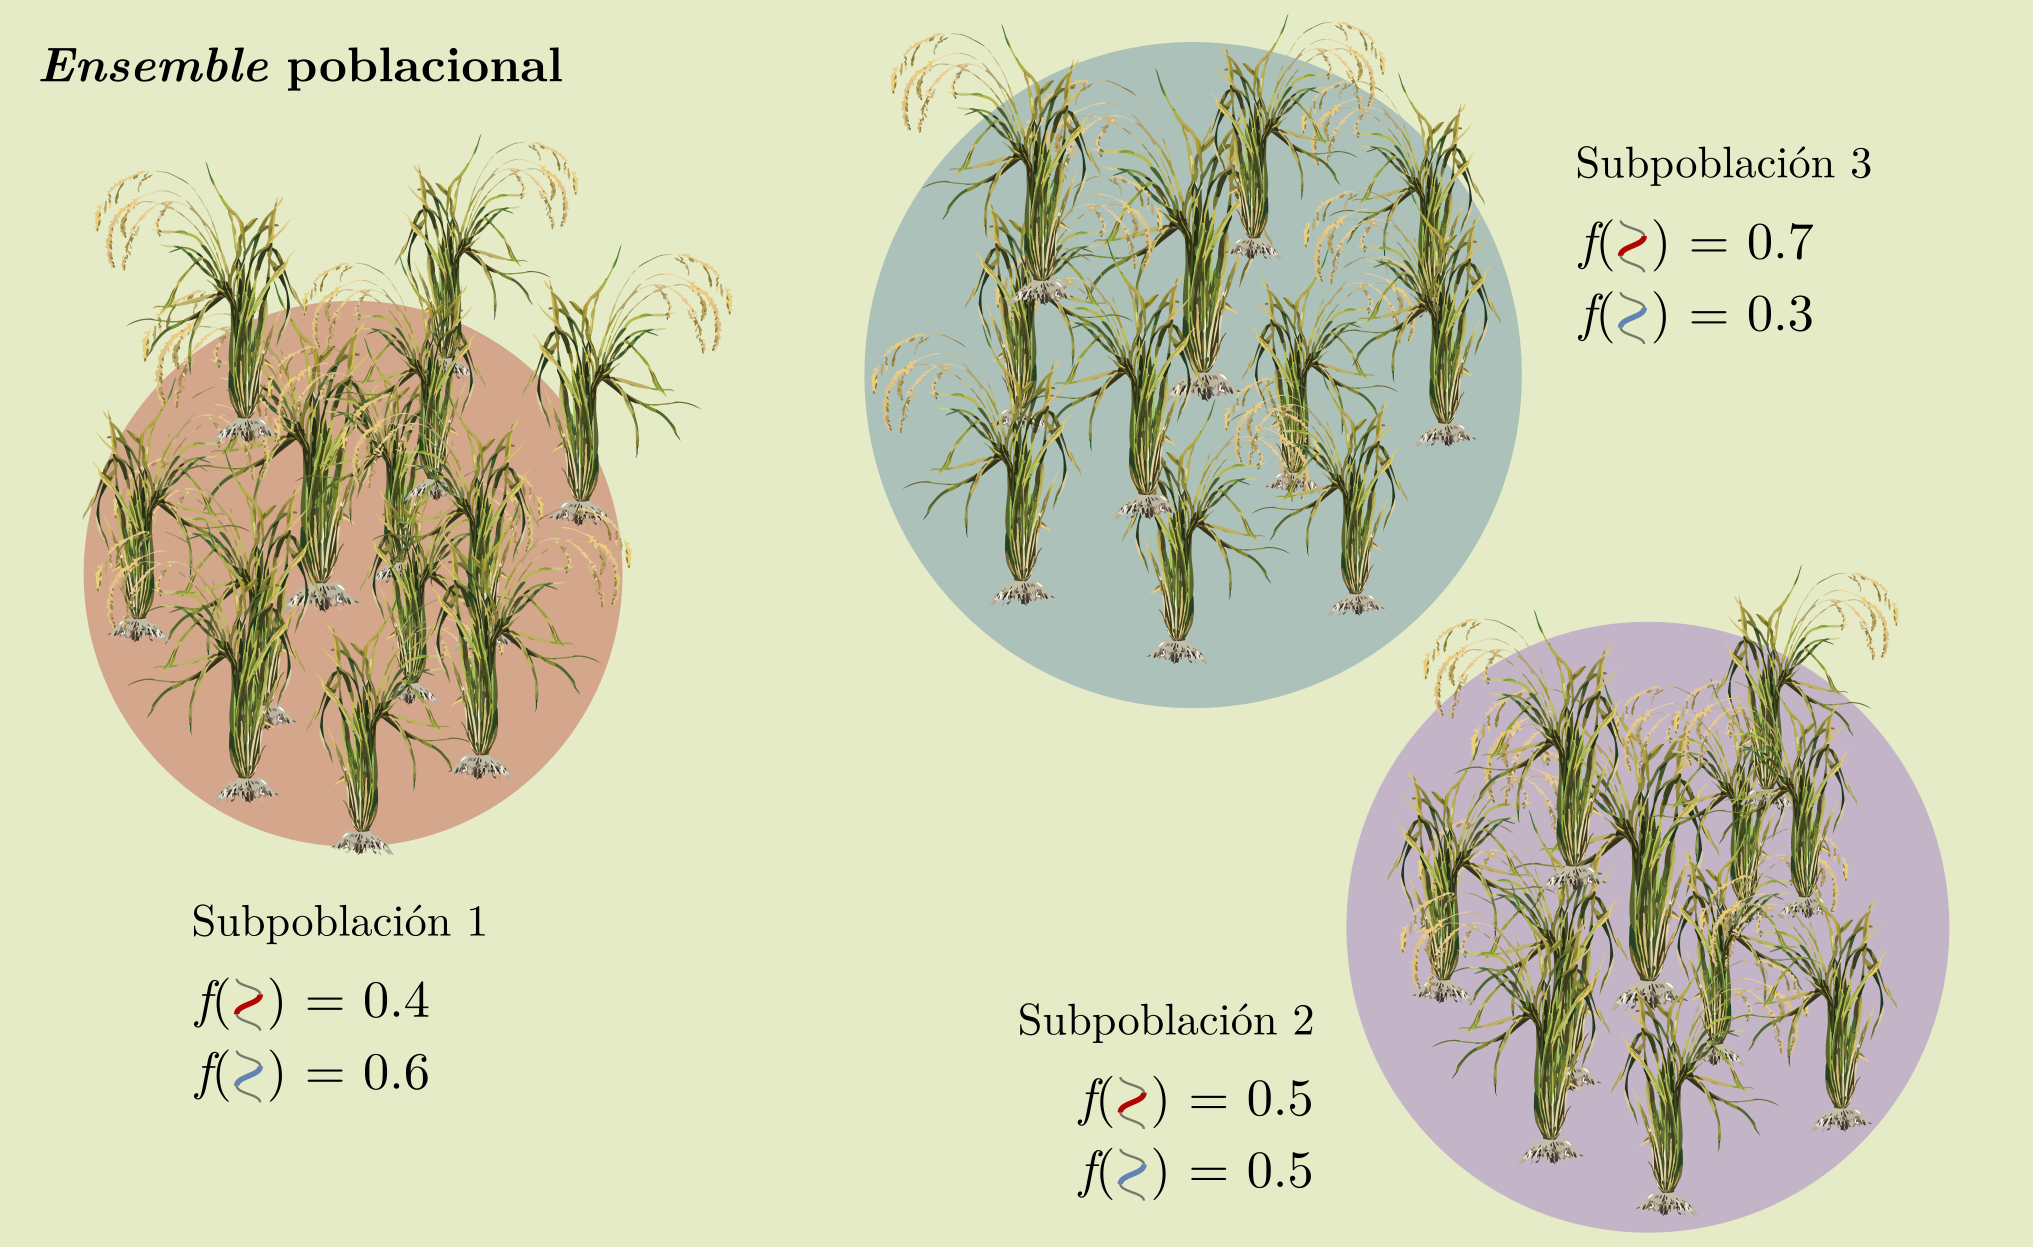
\includegraphics[width=1\linewidth]{figuras/ensemble} 

}

\caption{Ejemplo de \textit{ensemble} poblacional. Tres poblaciones de arroz (\textit{Oryza sativa}) se encuentran distribuídas en parches, a distancias tales que los individuos de cada subpoblación sólo se reproducen entre sí. Por efecto de la deriva genética es esperable que las frecuencias alélicas de las subpoblaciones del *ensemble* diverjan con el tiempo, lo cual se ejemplifica para un locus bialélico (alelos "rojo" y "azul", en la figura). Imagen creada con elementos gráficos tomados de bioicons (https://bioicons.com/).}\label{fig:ensemble}
\end{figure}

Suponiendo además que el tamaño efectivo (\(N_e\)) es relativamente pequeño, algo muy razonable teniendo en cuenta que los individuos deben reproducirse en su entorno cercano, estamos entonces en una situación como alguna de las representadas en la Figura \ref{fig:figura3p5}. Es decir, mientras que en algunos parches la frecuencia del alelo \textbf{A} crecerá hacia la fijación del mismo, en otras poblaciones posiblemente se pierda (o lo que es lo mismo, quede fijado el alelo \textbf{a}). Pero la deriva genética es un fenómeno que ocurre simultáneamente en todo el genoma (obviamente que en sitios \textbf{no ligados} del genoma el fenómeno es independiente) y por lo tanto aún las poblaciones que terminen con el alelo \textbf{A} fijado serán diferentes en otros \emph{loci}, donde la deriva ocurre en forma independiente. Todo este proceso, dado simplemente por la ``reglas'' de la reproducción, producirá un conjunto de poblaciones cada vez más disimiles entre ellas (y cada vez más parecidas dentro), lo que es un buen comienzo para la especiación.

Un fenómeno usual en muchas especies, que magnifica el rol de la deriva genética, es lo que se conoce como \textbf{cuello de botella poblacional} (o ``\emph{genetic bottleneck}'', en inglés). En efecto, en muchas especies es frecuente encontrarse con eventos que llevan a la casi extinción de alguna población en particular, en un momento dado del tiempo, luego de lo cual la población comienza a recuperarse e incrementar el número de individuos. Sin embargo, las huellas de esta momentánea reducción drástica son normalmente imborrables en el genoma. Como en el momento de máxima restricción solo unos pocos individuos sobreviven (constituyendo la base reproductiva de la población a futuro), al ser \(N_e\) muy pequeño la varianza por generación será enorme, además de que la frecuencia inicial de las variantes será posiblemente \textbf{sesgada} respecto a la misma población antes del cuello de botella. Esto último nos lleva directamente a otro fenómeno estrechamente relacionado: el \textbf{efecto fundador}.

El \textbf{efecto fundador} (Figura \ref{fig:efecto-fundador}) se produce cuando un número relativamente pequeño de individuos \textbf{funda una nueva población} y por efecto de la frecuencia sesgada en esa pequeña muestra más el efecto de la endogamia (o ``\emph{inbreeding}'', el efecto del apareamiento entre parientes que veremos en otro capítulo más adelante) casi obligada por el número reducido de individuos, llevan a medida de que la población va creciendo a una fuerte desviación de las frecuencias alélicas respecto a la población original.

\begin{figure}[H]

{\centering 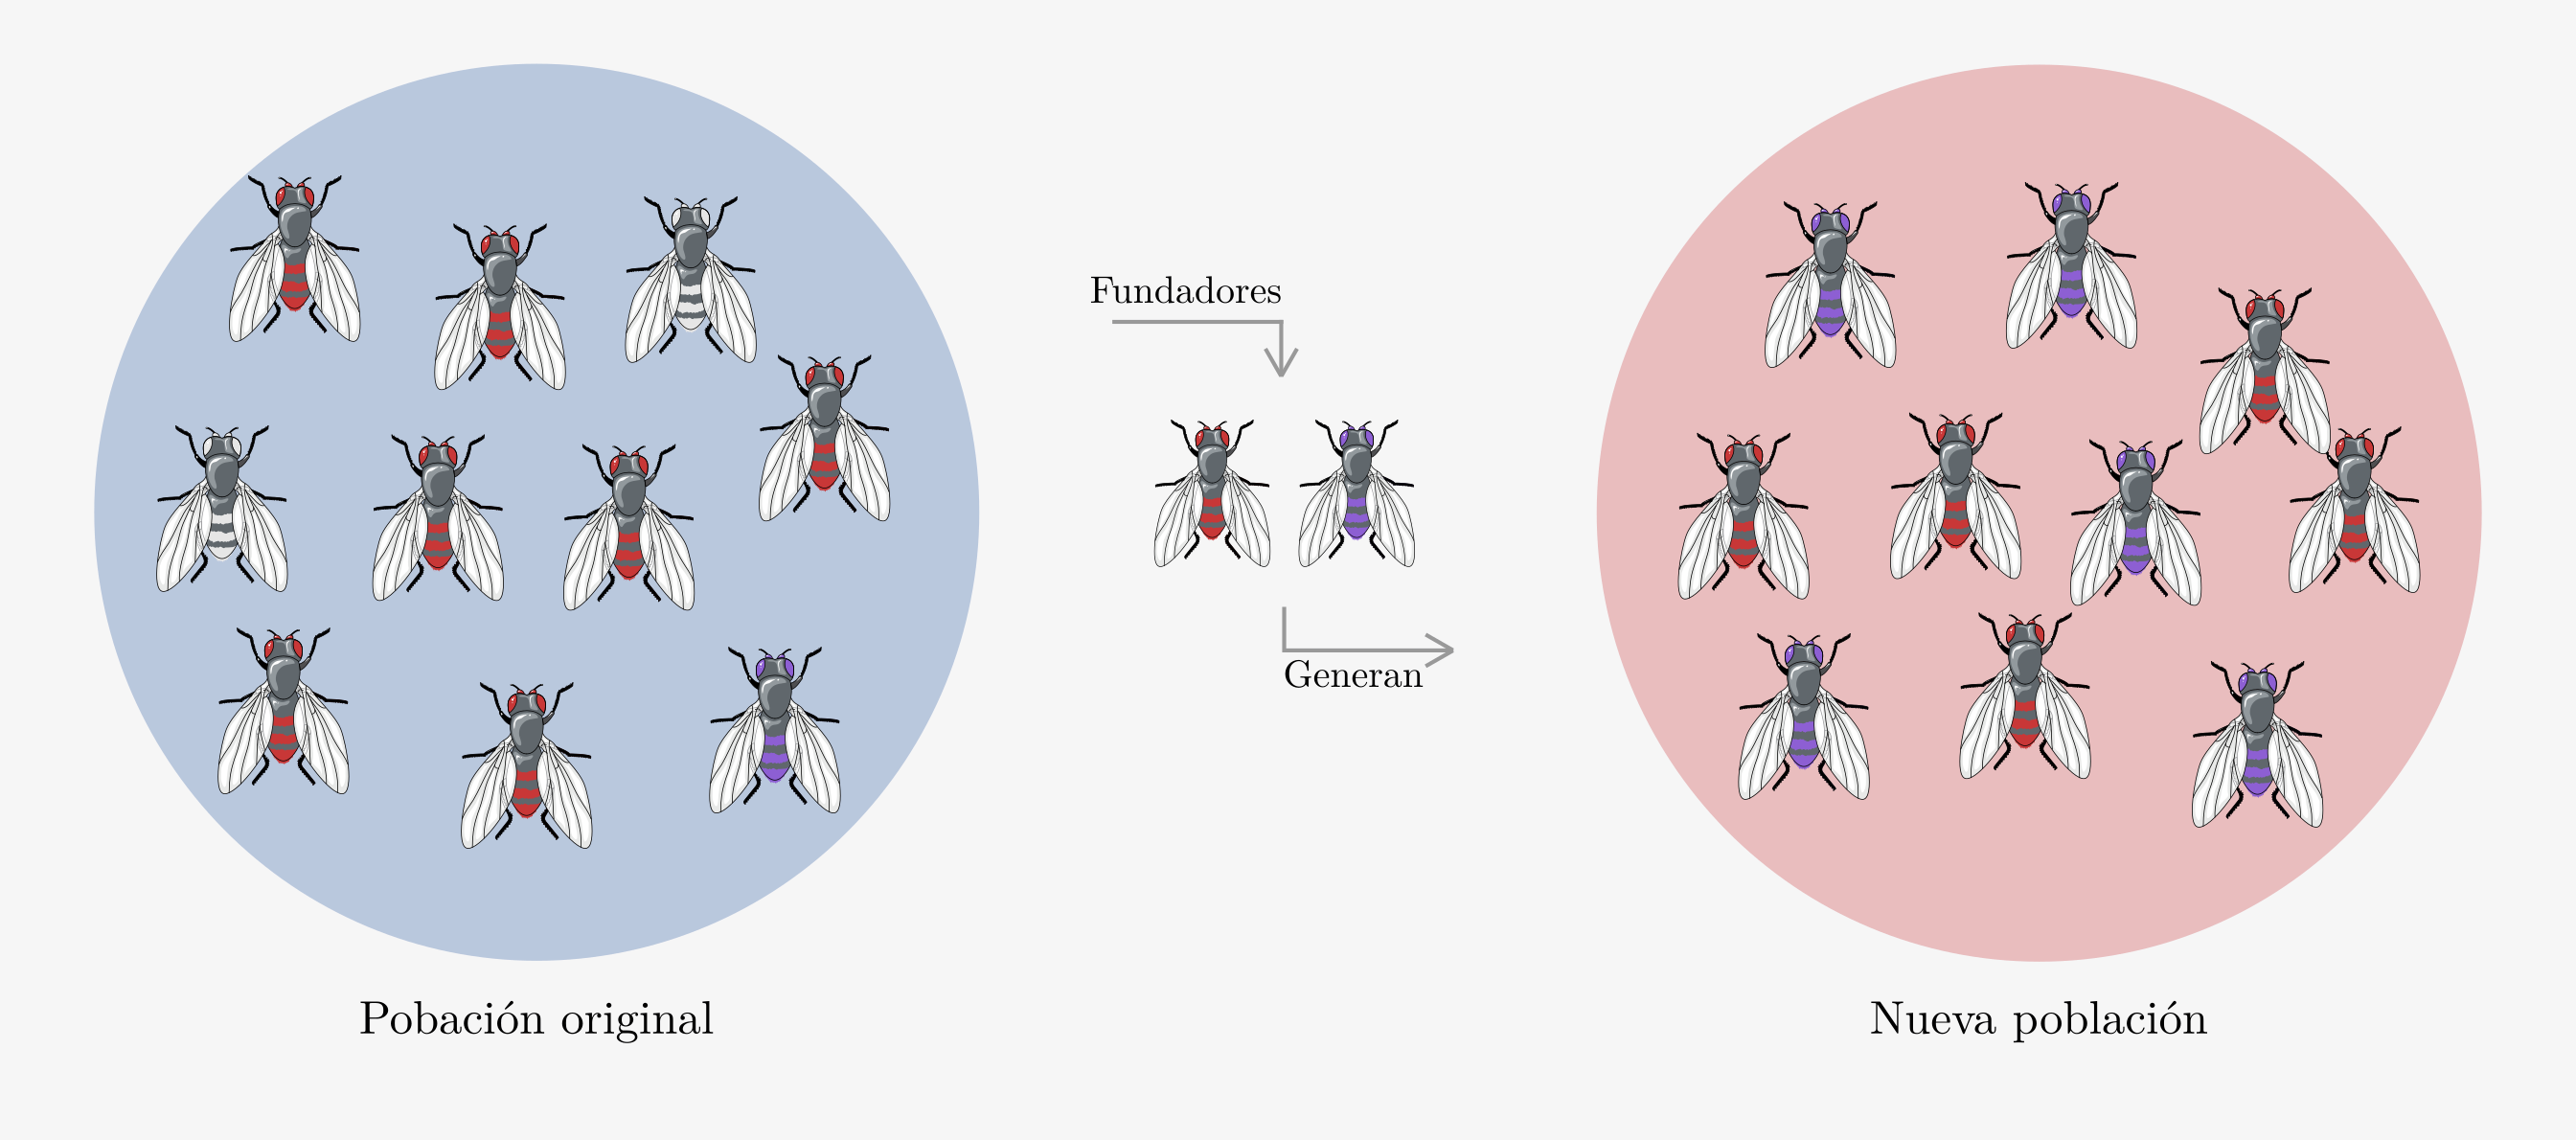
\includegraphics[width=1\linewidth]{figuras/efecto_fundador} 

}

\caption{Efecto fundador ejemplificado para una población de la mosca de la fruta (*D. melanogaster*). Cuando una nueva población es formada a partir de una muestra pequeña de individuos, las frecuencias alélicas presentes entre los individuos fundadores tendrán un fuerte impacto en el devenir de las frecuencias alélicas de la nueva población. Debido al efecto de muestreo, las frecuencia alélicas entre los miembros fundadores pueden apartarse considerablemente de las presentes en la población original. En el ejemplo vemos una población original de moscas que presentan diferentes fenotipos para el color de ojo (rojo, blanco y violeta), los cuales se asumen se deben a las variantes alélicas que presenta cada individuo en un locus. La muestra de individuos fundadores se encuentra fuertemente sesgada (la componen en igual proporción individuos con ojos rojos y violetas), lo cual lleva a que la nueva población fundada sea radicalmente diferente a la original. Imagen creada con elementos gráficos tomados de bioicons (https://bioicons.com/).}\label{fig:efecto-fundador}
\end{figure}

Un ejemplo notable entre poblaciones humanas lo constituye el pueblo de \textbf{Cândido Godói}, un municipio de Río Grande do Sul (Brasil) de unos 6 mil habitantes. El sobrenombre del pueblo es ``Terra dos gêmeos'' (tierra de los gemelos), ya que 1 de cada 10 mujeres ha tenido mellizos/gemelos, una cifra muy superior al 1,8\% de Río Grande do Sul (y en algún estudio, cerca de la mitad fueron monocigóticos), Figura \ref{fig:CandidoGodoi}.

\begin{figure}[H]

{\centering \includegraphics[width=0.6\linewidth]{figuras/candido_godoi} 

}

\caption{Mellizos/gemelos de Cândido Godoi (imagen sacada de la web, sin crédito de autor).}\label{fig:CandidoGodoi}
\end{figure}

Si bien se especuló que el origen de este fenómeno serían una serie de experimentos del doctor nazi Josef Mengele, la causa más probable es el estrecho parentesco de sus habitantes, unido al efecto fundador como origen de la colonia (\citeproc{ref-TaglianiRibeiro2011}{Tagliani-Ribeiro et al. 2011}). En particular, en este estudio los autores encuentran una fuerte asociación entre la presencia del alelo P72 en el gen \emph{TP53} y el ``riesgo'' de embarazo gemelar. También los autores reportan una significancia menor para la asociación entre el alelo T del gen \emph{MDM4} y en conjunto proponen que ambos alelos (en dos genes distintos) estarían actuando mediante la reducción del mecanismo de apoptosis inducida por p53.

\subsection*{Homocigosidad y heterocigosidad}\label{homocigosidad-y-heterocigosidad}
\addcontentsline{toc}{subsection}{Homocigosidad y heterocigosidad}

En las secciones anteriores nos hemos manejado considerando exclusivamente la evolución en el tiempo de las frecuencias alélicas en las distintas poblaciones que conforman nuestro \textbf{ensemble} y dejamos de lado el análisis de lo que ocurriría dentro y entre ellas desde el punto de vista de los genotipos. Consideremos, como una suposición \emph{a priori} razonable, que dentro de cada población se mantiene el apareamiento al azar y que más allá del número posiblemente pequeño de individuos dentro de ellas que hacen fluctuar las frecuencias alélicas, podemos esperar que las mismas se comporten \textbf{aproximadamente} según lo esperado en el equilibrio de Hardy-Weinberg de generación en generación. Para graficar nuestra situación supongamos que tenemos una gran población, con una frecuencia del alelo \textbf{A} igual a \(p=\frac{1}{2}=0,5\) que en el momento inicial de nuestra historia se divide en 4 poblaciones idénticas en tamaño (cada una de \(1/4\) del tamaño de la grande), como lo representamos en la Figura \ref{fig:subdivPob}. Cada una de estas poblaciones, a medida de que pase el tiempo, por efecto exclusivo de la deriva genética se irá apartando de la frecuencia original \(p=0,5\) y la varianza de frecuencias entre ellas irá creciendo en el tiempo, como vimos más arriba. Es de destacar que nuestra representación en la Figura \ref{fig:subdivPob} es apenas una configuración posible de infinitas, ya que la evolución de las 4 poblaciones será aleatoria, pero esta configuración en particular, sin pérdida de generalidad, nos ayudará a ilustrar el fenómeno general.

\begin{figure}[H]

{\centering 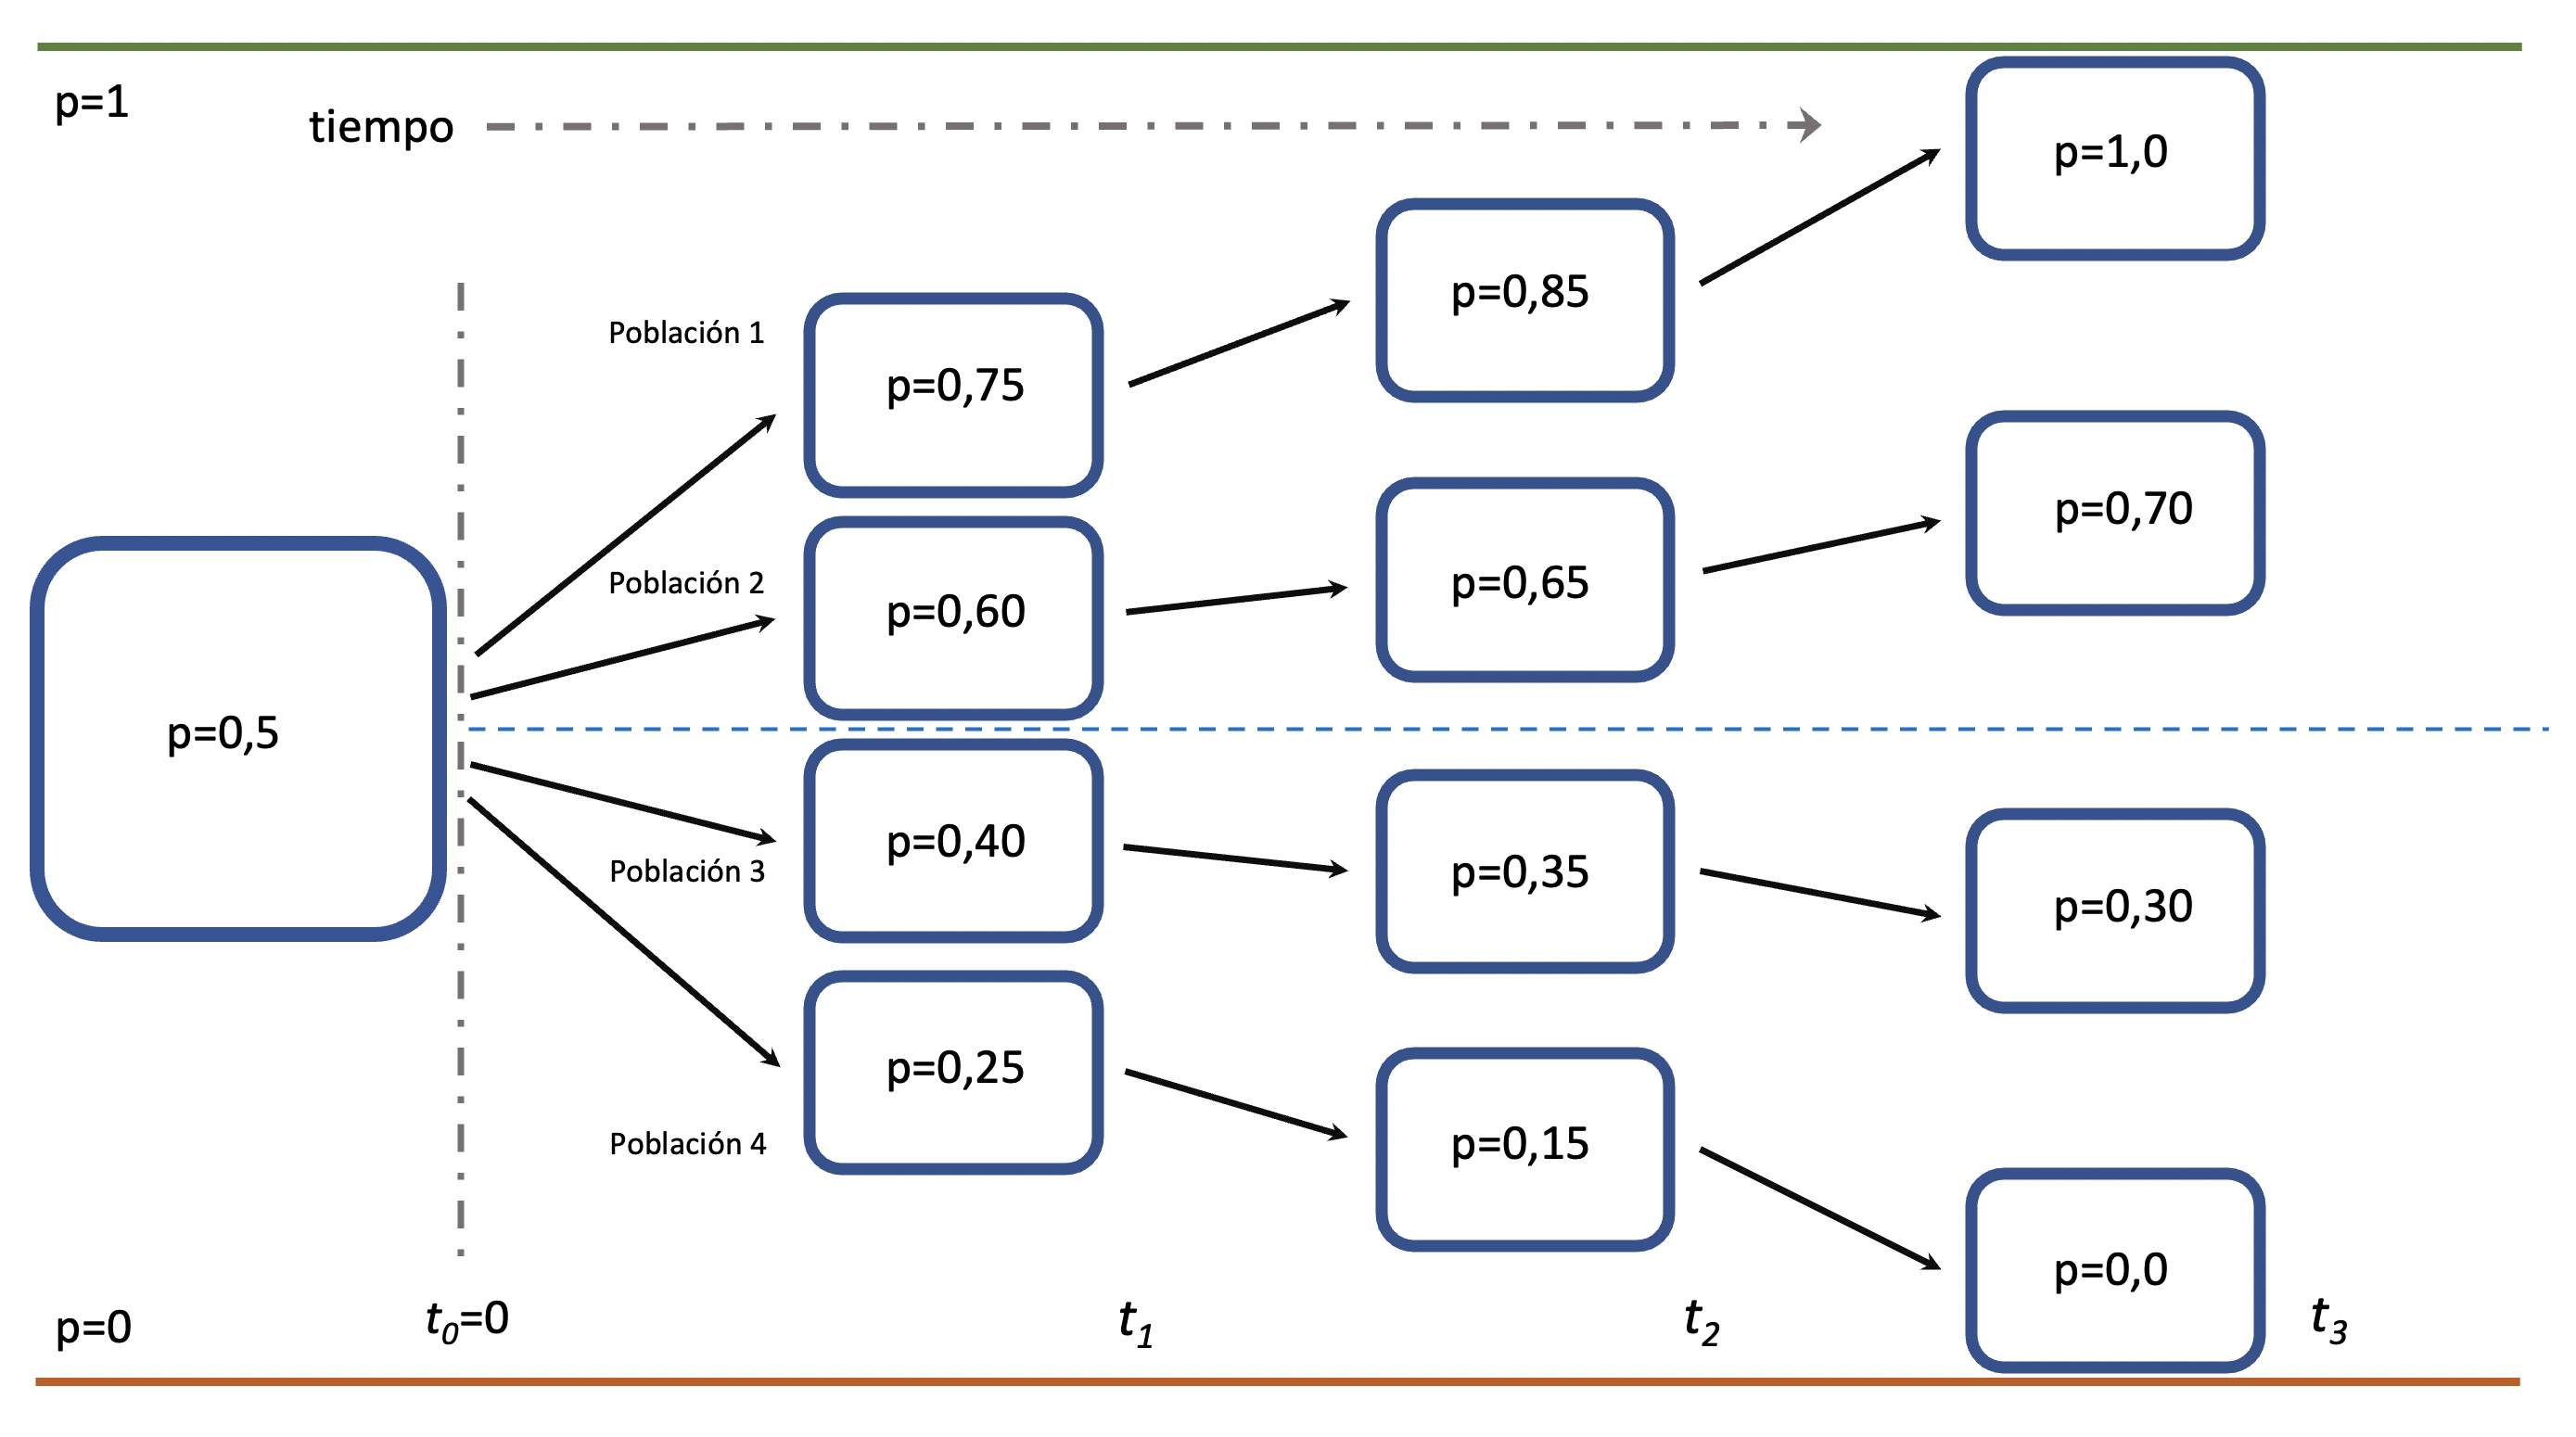
\includegraphics[width=0.8\linewidth]{figuras/subdivisionPoblacional2} 

}

\caption{Evolución por deriva genética de las frecuencias alélicas en 4 subpoblaciones que parten de la misma frecuencia (el tiempo no está a escala). Las líneas superior e inferior representan las   extbf{barreras absorbentes} de fijación y pérdida del alelo. A medida que corre el tiempo las poblaciones se apartan de la frecuencia alélica inicial, aunque se mantiene la frecuencia promedio como el valor inicial.}\label{fig:subdivPob}
\end{figure}

Si pensamos en la población original, antes de la subdivisión y asumimos que se encontraba en equilibrio de Hardy-Weinberg, ya que \(q=1-p=1-\frac{1}{2}=\frac{1}{2}\), tenemos que la composición de los tres genotipos era la siguiente:

\[
\begin{split}
AA=p^2=\left(\frac{1}{2}\right)^2=\frac{1}{4}\\
Aa=2pq=2 \cdot \frac{1}{2} \frac{1}{2}=2 \cdot \frac{1}{4}=\frac{1}{2}\\
aa=q^2=\left(\frac{1}{2}\right)^2=\frac{1}{4}
\end{split}
\]

Luego, con el paso del tiempo, llegamos a un determinado momento \(t_1\) en que las frecuencias alélicas ya han divergido algo. En la Tabla \ref{tab:subdivtx1} podemos ver lo que ocurre a nivel de los genotipos en cada una de las 4 poblaciones, así como la media de las 4 poblaciones (que como son todas iguales en tamaño es directamente igual al promedio de los valores). En la última columna tenemos también la frecuencia de los genotipos homocigotos, es decir \textbf{AA} y \textbf{aa}. Claramente, la frecuencia alélica promedio no ha cambiado, era de \(\frac{1}{2}\) en \(t_0=0\) y sigue siendo \(\frac{1}{2}\) en \(t_1\). Sin embargo, dentro de las poblaciones el cambio de frecuencia, sumado al equilibrio Hardy-Weinberg para cada una de ellas se refleja en diferencias importantes entre poblaciones en la proporción de homocigotos. Más aún, el promedio de los homocigotos (el promedio de la suma \textbf{AA} y \textbf{aa} en cada población) se vio incrementado, desde \(fr(AA)+fr(aa)=\frac{1}{4}+\frac{1}{4}=\frac{1}{2}=0,5\) a \(0,5725\). Este hecho no es menor: sin cambiar el promedio de las frecuencias alélicas y manteniendo el equilibrio de Hardy-Weinberg dentro de las poblaciones, si las volviésemos a agrupar a el solo efecto de contar los genotipos, el \textbf{ensemble} ya no se encuentra en el equilibrio de Hardy-Weinberg (porque el equilibrio para \(p=0,5\) es de \(G=\frac{1}{2}=0,5\)) \footnote{Notar que se utiliza el símbolo \(G\) para denotar al conjunto de genotipos homocigotos, como en la sección \hyperref[tres-o-muxe1s-alelos]{Tres o más alelos} del capítulo anterior.}.

\begin{table}
\centering
\caption{\label{tab:subdivtx1}Frecuencias de los genotipos en las 4 poblaciones, manteniendo el equilibrio de Hardy-Weinberg en cada una de ellas, en el primer punto en el tiempo luego del inicio ($t_1$).}
\centering
\begin{tabular}[t]{l|r|r|r|r|r}
\hline
  & p & AA & Aa & aa & Homocigotos\\
\hline
\cellcolor{gray!10}{Población 1} & \cellcolor{gray!10}{0,75} & \cellcolor{gray!10}{0,5625} & \cellcolor{gray!10}{0,3750} & \cellcolor{gray!10}{0,0625} & \cellcolor{gray!10}{0,6250}\\
\hline
Población 2 & 0,60 & 0,3600 & 0,4800 & 0,1600 & 0,5200\\
\hline
\cellcolor{gray!10}{Población 3} & \cellcolor{gray!10}{0,40} & \cellcolor{gray!10}{0,1600} & \cellcolor{gray!10}{0,4800} & \cellcolor{gray!10}{0,3600} & \cellcolor{gray!10}{0,5200}\\
\hline
Población 4 & 0,25 & 0,0625 & 0,3750 & 0,5625 & 0,6250\\
\hline
\cellcolor{gray!10}{Media} & \cellcolor{gray!10}{0,50} & \cellcolor{gray!10}{0,2862} & \cellcolor{gray!10}{0,4275} & \cellcolor{gray!10}{0,2862} & \cellcolor{gray!10}{0,5725}\\
\hline
\end{tabular}
\end{table}

Veamos qué ocurre entonces a medida de que nos alejamos del punto inicial en el tiempo. Cuando llegamos al punto \(t_2\), las frecuencias en las poblaciones divergen un poco más, aunque ninguna población ha llegado aún a fijar alguno de los dos alelos. La distribución de los genotipos en las mismas, de acuerdo a las nuevas frecuencias alélicas, se puede apreciar en la Tabla \ref{tab:subdivtx2}. Claramente volvemos a ver un incremento en promedio de homocigotos en la población, que ahora alcanzó el valor \(0,6450\).

\begin{table}
\centering
\caption{\label{tab:subdivtx2}Frecuencias de los genotipos en las 4 poblaciones, manteniendo el equilibrio de Hardy-Weinberg en cada una de ellas, en el segundo punto en el tiempo luego del inicio ($t_2$).}
\centering
\begin{tabular}[t]{l|r|r|r|r|r}
\hline
  & p & AA & Aa & aa & Homocigotos\\
\hline
\cellcolor{gray!10}{Población 1} & \cellcolor{gray!10}{0,85} & \cellcolor{gray!10}{0,7225} & \cellcolor{gray!10}{0,255} & \cellcolor{gray!10}{0,0225} & \cellcolor{gray!10}{0,745}\\
\hline
Población 2 & 0,65 & 0,4225 & 0,455 & 0,1225 & 0,545\\
\hline
\cellcolor{gray!10}{Población 3} & \cellcolor{gray!10}{0,35} & \cellcolor{gray!10}{0,1225} & \cellcolor{gray!10}{0,455} & \cellcolor{gray!10}{0,4225} & \cellcolor{gray!10}{0,545}\\
\hline
Población 4 & 0,15 & 0,0225 & 0,255 & 0,7225 & 0,745\\
\hline
\cellcolor{gray!10}{Media} & \cellcolor{gray!10}{0,50} & \cellcolor{gray!10}{0,3225} & \cellcolor{gray!10}{0,355} & \cellcolor{gray!10}{0,3225} & \cellcolor{gray!10}{0,645}\\
\hline
\end{tabular}
\end{table}

Para ser breves y confirmar la tendencia observada (además de comenzar a imaginar hacia dónde nos lleva ésta), veamos qué ocurre en el instante \(t_3\). Llegado este momento, en la \emph{Población 1} se ha fijado el alelo \textbf{A} (\(p=1\)), mientras que en la \emph{Población 4} se ha fijado el alelo \textbf{a} (o lo que es equivalente, se ha perdido el \textbf{A}, \(p=0\)). La distribución de genotipos se observa en la Tabla \ref{tab:subdivtx3}.

\begin{table}
\centering
\caption{\label{tab:subdivtx3}Frecuencias de los genotipos en las 4 poblaciones, manteniendo el equilibrio de Hardy-Weinberg en cada una de ellas, en el tercer punto en el tiempo luego del inicio ($t_3$).}
\centering
\begin{tabular}[t]{l|r|r|r|r|r}
\hline
  & p & AA & Aa & aa & Homocigotos\\
\hline
\cellcolor{gray!10}{Población 1} & \cellcolor{gray!10}{1,0} & \cellcolor{gray!10}{1,000} & \cellcolor{gray!10}{0,00} & \cellcolor{gray!10}{0,000} & \cellcolor{gray!10}{1,00}\\
\hline
Población 2 & 0,7 & 0,490 & 0,42 & 0,090 & 0,58\\
\hline
\cellcolor{gray!10}{Población 3} & \cellcolor{gray!10}{0,3} & \cellcolor{gray!10}{0,090} & \cellcolor{gray!10}{0,42} & \cellcolor{gray!10}{0,490} & \cellcolor{gray!10}{0,58}\\
\hline
Población 4 & 0,0 & 0,000 & 0,00 & 1,000 & 1,00\\
\hline
\cellcolor{gray!10}{Media} & \cellcolor{gray!10}{0,5} & \cellcolor{gray!10}{0,395} & \cellcolor{gray!10}{0,21} & \cellcolor{gray!10}{0,395} & \cellcolor{gray!10}{0,79}\\
\hline
\end{tabular}
\end{table}

Ahora, además de haber aumentado nuevamente la proporción de homocigotos respecto al punto anterior en el tiempo, también tenemos un fenómeno nuevo: dos poblaciones solo tienen (y tendrán a futuro) genotipos homocigotos, ya que se ha fijado uno de los dos alelos. Todo esto ocurre sin cambiar la frecuencia alélica media del \textbf{ensemble}. Más aún, si recordamos el comportamiento de las frecuencias alélicas en el tiempo, tarde o temprano las poblaciones terminan cayendo en alguna de las dos ``trampas'' que son las \textbf{barreras absorbentes}, los estados de fijación o pérdida (fijación del otro alelo), por lo que este comportamiento de la \emph{Población 1} y \emph{Población 4} es también esperable para las otras dos poblaciones (veremos este fenómeno en detalle más adelante). Llegado ese momento ya no quedarán heterocigotos en el \textbf{ensemble}, pese a que la frecuencia alélica se mantiene como al inicio.

Para entender mejor y poder cuantificar este fenómeno de la reducción del número de heterocigotos debemos pasar a entender primero algunos conceptos sobre los que ahondaremos más adelante (ver capítulo \hyperref[aparnoalazar]{Apareamientos no-aleatorios}). Como vimos previamente, el concepto de alelo ha ido variando en el tiempo a medida de que nuestro conocimiento sobre la biología molecular y la genética han llevado a entender las bases de la variación genética. Sin embargo, hay un aspecto en que las cosas no han cambiado mucho: el origen de la similaridad o diferencia entre alelos. En ausencia de mutación\footnote{La persona interesada en el modelado e implicancias de la relación entre mutación y deriva genética puede referirse a la bibliografía de referencia, donde suele tratarse dicho tema. A lo largo de este capítulo se deja este aspecto de lado, a efectos de simplificar el análisis y hacer foco en el fenómeno de la deriva genética.}, cuando un alelo es diferente de otro en la presente generación, nos resulta obvio de dónde viene la diferencia: dos alelos son diferentes en esta generación porque provienen de diferentes alelos en la generación previa, y hay poca distinción más que agregar. Sin embargo, cuando dos alelos son ``iguales'' (decimos que es el mismo alelo) en la presente generación, podemos ser más precisos sobre el origen de esta similitud: los dos alelos ``iguales'' en la presente generación pueden provenir de dos alelos ``iguales'' en la generación previa, pero que no sean copias del mismo ADN que los generó, o pueden ser copias del mismo ADN (gametos del mismo individuo y del mismo cromosoma), en cuyo caso los llamamos \textbf{idénticos por ascendencia}. Este concepto es fundamental, así que asegúrate de haberlo entendido. En ambos casos, cuando los dos alelos son ``iguales'' independientemente del origen, decimos que son \textbf{idénticos en estado}. Claramente, excepto por mutaciones recurrentes en el tiempo, si nos retrotraemos en el pasado lo suficiente, todos los alelos \textbf{idénticos en estado} deberían venir del mismo alelo original, y por lo tanto serían de alguna manera \textbf{idénticos por ascendencia}, por lo que el marco de referencia es fundamental para decidir a partir de cuando se comienza a hacer esta distinción.

La probabilidad de que \textbf{los dos alelos en un individuo} sean \textbf{idénticos por ascendencia} se simboliza comúnmente con la letra \(F\), a partir de Sewall Wright (\citeproc{ref-wright1922}{1922}), que lo llamó \textbf{coeficiente de fijación}. Nosotros vamos a utilizar un subíndice para denotar el tiempo desde la generación \(0\), que consideramos la generación inicial. Supongamos que queremos calcular la probabilidad de que dos alelos sean \textbf{idénticos por ascendencia} en la generación \(t\), es decir \(F_t\).



\begin{figure}[H]

{\centering 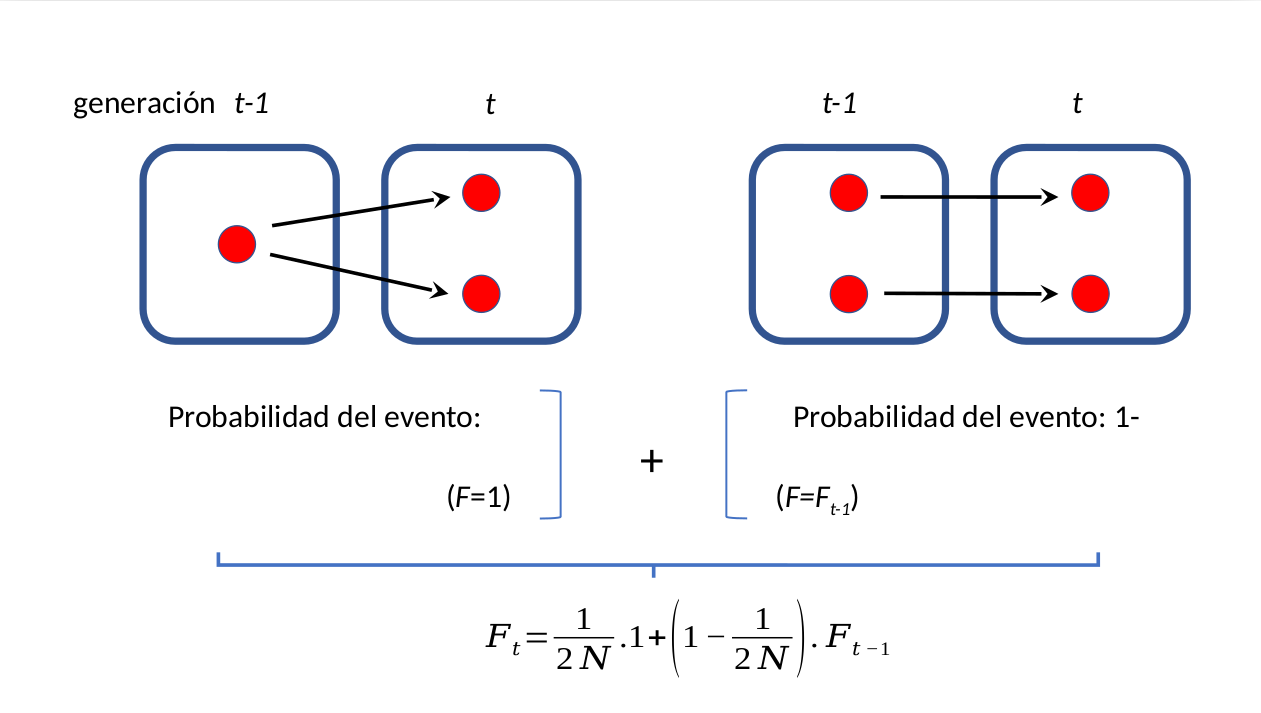
\includegraphics[width=0.8\linewidth]{figuras/recursionFt2} 

}

\caption{Ilustración del razonamiento detrás de la recursión para \emph{F} en una población de tamaño finito. Existen dos alternativas disjuntas (de ahí la suma) para que un alelo sea idéntico por ascendencia en la generación \emph{t}: que los alelos provengan del mismo alelo en la generación \emph{t-1}, cuya probabilidad es \(\frac{1}{2N}\) (y en ese caso \(F=1\), por definición) o que los alelos provengan de distintas copias en la generación \emph{t-1}, y en cuyo caso la probabilidad de que sean idénticos por ascendencia es por definición \(F_{t-1}\). Por lo tanto, la probabilidad de que dos alelos sean idénticos por ascendencia en la generación \(t\), considerando a la generación \(t-1\), es de \(F_t=\frac{1}{2N}+\left(1-\frac{1}{2N}\right) F_{t-1}\). Aplicando este razonamiento a las sucesivas generaciones anteriores se puede obtener, por recursión, la probabilidad de que dos alelos sean ídénticos por ascendencia a tiempo \(t\) (tomando como referencia la población a tiempo \(t=0\)).}\label{fig:recursionFt}
\end{figure}

Como se ilustra en la Figura \ref{fig:recursionFt}, existen dos posibilidades mutuamente excluyentes para que dos alelos sean \textbf{idénticos por ascendencia} en la generación \(t\): \emph{a)} que los dos alelos provengan del mismo alelo en la generación \(t-1\), un evento cuya probabilidad es \(\frac{1}{2N}\) (ya que hay \(2N\) alelos en la población y por lo tanto la probabilidad de volver a muestrear el mismo es \(\frac{1}{2N}\)) y en ese caso \(F=1\), ya que al venir del mismo alelo este es \textbf{idéntico por ascendencia} a sí mismo con probabilidad de 1, y \emph{b)} que los alelos provengan de distintas copias en la generación \(t-1\), y en ese caso la probabilidad de que sean \textbf{idénticos por ascendencia} es por definición \(F_{t-1}\). Como se trata de dos eventos disjuntos (puede pasar uno u otro, pero no los dos a la vez), puedo sumar sus probabilidades para tener

\begin{equation}
F_t=\frac{1}{2N}+\left(1-\frac{1}{2N}\right)F_{t-1}
\label{eq:recursionF1}
\end{equation}

Se puede calcular así la probabilidad de dos alelos sean \textbf{idénticos por ascendencia} en una generación, asumiendo que se conoce dicha probabilidad para la generación anterior. Veamos ahora si podemos llegar a una expresión general para la probabilidad de dos alelos sean \textbf{idénticos por ascendencia} en una generación basado en el número de generaciones transcurridas desde un momento de referencia (\(t=0\)) y la probabilidad inicial \(F_0\) en dicho momento. Si a ambos lados de la ecuación \eqref{eq:recursionF1} multiplicamos por \(-1\) y le sumamos \(1\) \footnote{Esta operación matemática puede resultar arbitraria. ¿Por qué haríamos esto? ¿Existe algún razonamiento biológico que de sustento a la maniobra? Notemos que \((1 - F_t)\) es la probabilidad de que dos alelos \emph{no} sean idénticos por ascendencia en el tiempo \(t\). Por lo tanto, la utilización de esta maniobra matemática simplifica los cálculos, pero además puede ser vista como un intento de resolver el problema planteandoló desde una óptica biológica ``complementaria''. Si resolvemos qué sucede con la probabilidad de que dos alelos \emph{no} sean idénticos por ascendencia, automáticamente resolvemos qué sucede con la probabildad de que si lo sean, por ser estos eventos disjuntos. La relación entre \(F\) y desviación de la heterocigosidad esperada es analizada más adelante en este capítulo.} tenemos

\begin{equation}
1-F_t=1-\frac{1}{2N}-(1-\frac{1}{2N}) F_{t-1}
1-F_t=(1-\frac{1}{2N})(1-F_{t-1})
\label{eq:recursionF2}
\end{equation}

Pero con la misma lógica,

\begin{equation}
1-F_{t-1}=\left(1-\frac{1}{2N}\right)(1-F_{t-2})
\label{eq:recursionF3}
\end{equation}

y sustituyendo \eqref{eq:recursionF3} en \eqref{eq:recursionF2}, tenemos

\begin{equation}
1-F_t=(1-\frac{1}{2N})(1-\frac{1}{2N})(1-F_{t-2})=(1-\frac{1}{2N})^2(1-F_{t-2})
\label{eq:recursionF4}
\end{equation}

Prosiguiendo con la recursión hasta llegar a la generación \(0\) (generación inicial), como transcurren \(t\) generaciones entre la \(0\) y la actual tenemos que la ecuación \eqref{eq:recursionF4} se generaliza a

\begin{equationbox}
\begin{equation}
1-F_t=\left(1-\frac{1}{2N}\right)^t(1-F_{0})
\label{eq:recursionF5}
\end{equation}

\end{equationbox}

Más aún, si asignamos arbitrariamente \(F_0=0\) por falta de conocimiento acerca de la probabilidad de que dos alelos sean idénticos por ascendencia en la generación inicial, entonces la ecuación \eqref{eq:recursionF5} se transforma en

\begin{equation}
1-F_t=\left(1-\frac{1}{2N}\right)^t 
\end{equation}

\begin{equationbox}
\begin{equation}
F_t=1-\left(1-\frac{1}{2N}\right)^t
\label{eq:recursionF6}
\end{equation}

\end{equationbox}

Veamos ahora cómo se relaciona todo esto con el problema de la subdivisión poblacional planteado en la Figura \ref{fig:subdivPob}. Por definición, \(F\) es también la reducción en heterocigosis (o el incremento en homocigosis) respecto a la expectativa en equilibrio de Hardy-Weinberg (y sus frecuencias genotípicas) en poblaciones finitas (porque es la probabilidad de que dos alelos sean idénticos por ascendencia en un individuo, por lo tanto homocigoto). Entonces, el paralelismo de \(1-F\) es respecto a los heterocigotos conservados y el apareamiento aleatorio. Si consideramos que la frecuencia esperada de heterocigotas en una población de tamaño finito es una función de \(p\) y \(q\), pero también de esa probabilidad de que los alelos no sean idénticos por ascendencia, entonces si llamamos \(H_t\) a esa frecuencia, tenemos,

\[
\begin{split}a
H_t=2pq(1-F_{t-1})\\
\therefore 1-F_{t-1}=\frac{H_t}{2pq}
\end{split}
\]

El \(t-1\) en el término \((1-F_{t-1})\) se corresponde con el hecho de que el efecto de la reducción de los pares de alelos \textbf{NO idénticos por ascendencia} se ve en la generación anterior a la presente. Notemos que \(H_t = 2pq(1-F_{t-1})\), lo cual equivale a decir \(1-F_{t-1} = \frac{H}{2pq}\). Sustituyendo en \eqref{eq:recursionF5}

\[
1-F_t=\frac{H_t}{2pq}=\left(1-\frac{1}{2N}\right)(1-F_{t-1}) 
\]

O lo que es igual \(H_t = (1-\frac{1}{2N}) H_{t-1}\).

Podemos extender este razonamiento un número arbitrario de generaciones hacia atrás, hasta la generación inicial (conozcamos el valor de heterocigosidad \(H_0\) en esta o no). Aplicando este razonamiento recursivo tenemos

\[
H_t = (1 - \frac{1}{2N})^t H_0
\label{eq:recursionF7}
\]

Utilizando la aproximación \(-b^t \approx e^{-bt}\) (teniendo en cuenta que \((1-\frac{1}{2N}) \approx -\frac{1}{2N}\) cuando \(N\) es pequeño), tenemos

\begin{equationbox}
\begin{equation}
H_t=\left(1-\frac{1}{2N}\right)^t H_0 \approx H_0 e^{\frac{-t}{2N}}
\label{eq:recursionF8}
\end{equation}

\end{equationbox}

donde en el último paso se tiene en cuenta la siguiente aproximación: \((1-a)^b \approx (e^{-a})^b \approx e^{-ab}\) cuando \(a \to 0\) (en nuestro caso, \(a = \frac{1}{2N};\ b = t\)).

Es decir, pese a que en cada una de las poblaciones se mantiene el equilibrio de Hardy-Weinberg, como se puede apreciar en la Figura \ref{fig:figura3p9}, la proporción de individuos heterocigotos en el conjunto de ellas, o mejor dicho el promedio en el \textbf{ensemble}, decaerá en forma geométrica respecto al valor inicial a lo largo del tiempo ya que la proporción en cada generación es multiplicada por el factor \(\left(1-\frac{1}{2N}\right)\) al pasar a la siguiente. La aproximación exponencial funciona en general razonablemente bien, y permite resolver algunos problemas en forma más sencilla. El efecto de la reducción en la proporción de heterocigotos es realmente drástico cuando los tamaños poblacionales son extremadamente pequeños, por ejemplo \(N=5\) o \(N=10\) individuos en la Figura \ref{fig:figura3p9}, pero son apenas notables cuando el número de individuos es 50 o más (notar que para 100 individuos el punto de reducción a \(50\%\) de la heterocigosis inicial ni siquiera aparece en la gráfica, ya que llevaría más de 138 generaciones para alcanzarlo).

\begin{figure}[H]

{\centering 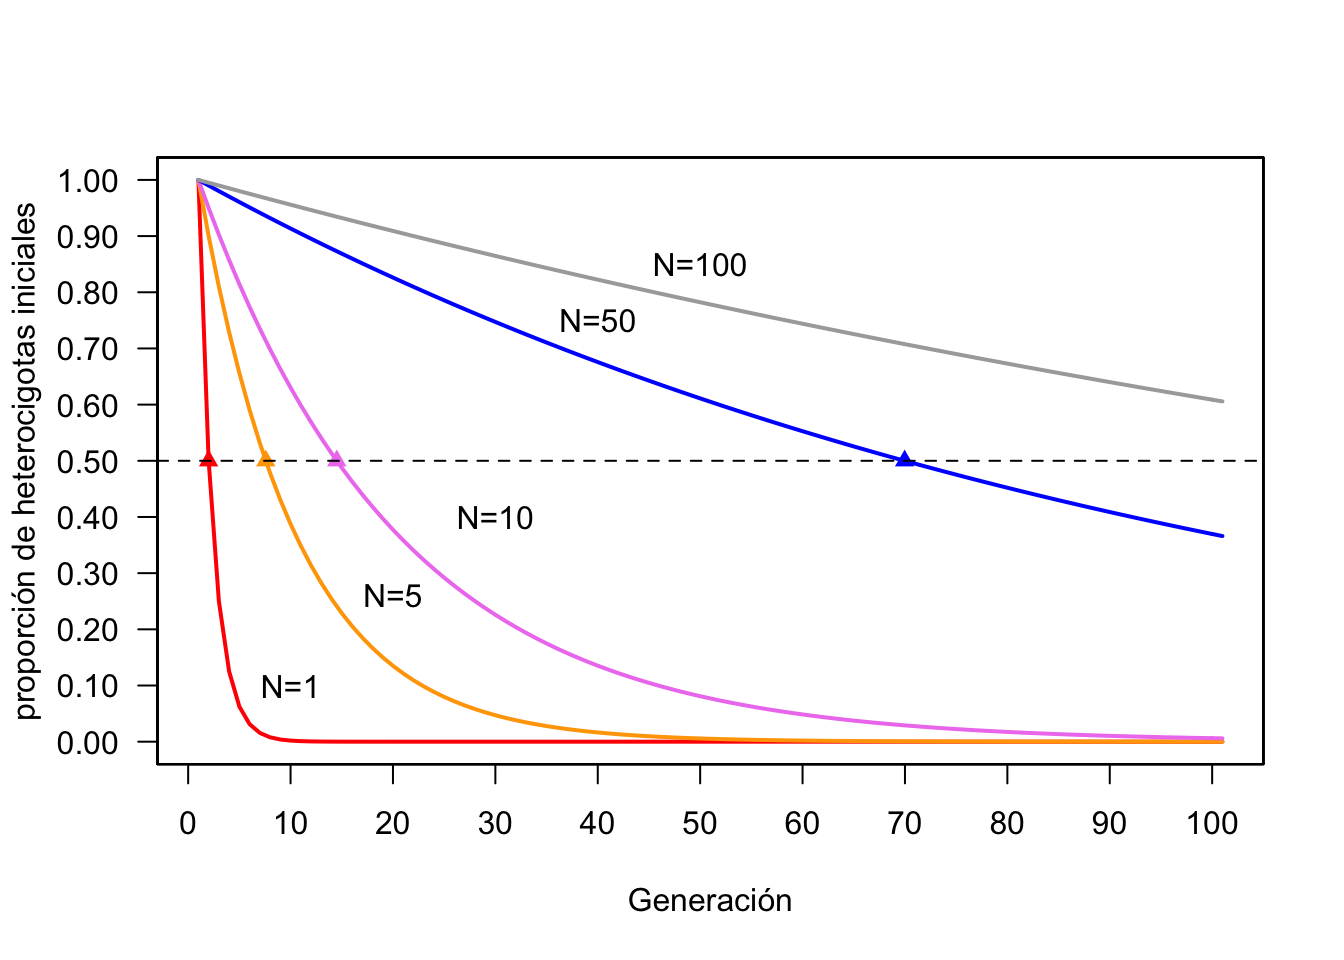
\includegraphics[width=0.7\linewidth]{ApuntesGeneticaII_files/figure-latex/figura3p9-1} 

}

\caption{Reducción esperada en el número inicial de heterocigotas $H_0$ de acuerdo al tamaño N de las poblaciones y al número de generaciones transcurridas. La línea negra horizontal marca la reducción a la mitad del valor inicial y los puntos sobre las curvas resaltan el número de generaciones requeridas para esa reducción a la mitad.}\label{fig:figura3p9}
\end{figure}

\subsection*{Ejemplo 3.2}\label{ejemplo-3.2}
\addcontentsline{toc}{subsection}{Ejemplo 3.2}

La ecuación \eqref{eq:recursionF8}, en particular la aproximación exponencial, nos permite estimar facilmente los tiempos hasta determinado nivel de reducción de la frecuencia inicial de heterocigotos. Por ejemplo, para alcanzar la mitad del valor inicial (\(H_0\)), con poblaciones de \(N\) individuos puedo hacer \(H_t=\frac{H_0}{2}\). Luego, de acuerdo a la ecuación \eqref{eq:recursionF8} tenemos que

\[
\begin{split}
H_t=\frac{H_0}{2}=H_0e^{\frac{-t}{2N}}\\
\therefore \frac{1}{2}=e^{\frac{-t}{2N}}
\end{split}
\]

Aplicando el logaritmo a ambos lados de la ecuación, tenemos

\begin{equation*}
\ln\left(\frac{1}{2}\right)=\ln\left(e^{\frac{-t}{2N}}\right)=\frac{-t}{2N}
\end{equation*}

y finalmente

\begin{equation*}
t=-2N \ln\left(\frac{1}{2}\right) \approx 1,39N
\end{equation*}

Es decir, en \(1,39N\) generaciones. Si lo hubiésemos hecho sin la aproximación, el procedimiento es análogo y llegaríamos a

\begin{equation*}
\frac{H_0}{2}=\left(1-\frac{1}{2N}\right)^t H_0 \therefore t=\frac{\ln{\left(\frac{1}{2}\right)}}{\ln{\left(1-\frac{1}{2N}\right)}}
\end{equation*}

que si bien es la solución exacta, no es lineal en el número de individuos en cada población.

\begin{center}\rule{0.5\linewidth}{0.5pt}\end{center}

Resumiendo, en esta sección vimos cómo la subdivision poblacional produce el efecto de disminuir el número de heterocigotas respecto a los esperado para las poblaciones del \textbf{ensemble} agregadas en un solo grupo y bajo condiciones de \textbf{panmixia} (es decir, con libertad de aparearse con cualquier otro individuo de la población, sin restricciones genéticas, conductuales o ambientales). Esa disminución de la proporción de heterocigotos esperados ocurre a una tasa constante por generación (en nuestro modelo) y la misma es de \(\left(1-\frac{1}{2N}\right)\), por lo que la reducción total a lo largo de \(t\) generaciones será del orden de \(\left(1-\frac{1}{2N}\right)^t\). Mientras que en la sección \hyperref[el-modelo-de-wright-fisher]{El modelo de Wright-Fisher} construimos un modelo de evolución de las frecuencias alélicas sin preocuparnos de los genotipos, en esta sección vimos las implicancias para la evolución de los genotipos tiene dicho modelo. En la sección \hyperref[cadenas-de-markov]{Cadenas de Markov} veremos de otra forma una conexión entre los dos fenómenos utilizando una aproximación fundamental para comprender los procesos estocásticos en general.

\begin{graybox}

\begin{itemize}
\tightlist
\item
  La recursión para el \textbf{coeficiente de fijación} \(F\) en la generación \(t\), \(F_t\) es igual a:
  \begin{equation*}
  1-F_t=\left(1-\frac{1}{2N}\right)^t(1-F_0)
  \end{equation*}
\item
  Cuando \(F_0=0\), es decir que asumimos que en la \textbf{generación inicial} la probabilidad de que dos alelos en un locus de un individuo diploide es cero, entonces la recursión anterior se simplifica a:
\end{itemize}

\begin{equation*}
F_t=1-\left(1-\frac{1}{2N}\right)^t
\end{equation*}

\begin{itemize}
\tightlist
\item
  El número de heterocigotos en un \textbf{ensemble} de poblaciones de tamaño finito \(N\) se ve reducido de generación en generación respecto a lo esperado para el equilibrio de Hardy-Weinberg. Esa reducción es a la tasa de \(\left(1-\frac{1}{2N}\right)\) por generación, por lo que la frecuencia de heterocigotos en la generación \(t\) se calcula de acuerdo a la siguiente ecuación:
\end{itemize}

\begin{equation*}
H_t=\left(1-\frac{1}{2N}\right)^t H_0 \approx H_0 e^{\frac{-t}{2N}}
\end{equation*}

\end{graybox}

\section{Cadenas de Markov}\label{cadenas-de-markov}

Si recuerdas la ecuación \eqref{eq:WrightFisher} de más arriba establecía la probabilidad de transición de un número \(i\) de copias a un número \(j\) (en un total de \(2N\) alelos) en una generación, y la misma era igual a:

\begin{equation}
T_{ij}={2N \choose j}\left(\frac{i}{2N}\right)^{j}\left(\frac{2N-i}{2N}\right)^{2N-j}=\frac{(2N)!}{j!(2N-j)!}p^jq^{2N-j}
\label{eq:WrightFisher2}
\end{equation}

Visto de otra forma, como \(i\) puede ir desde \(0\) hasta \(2N\) y lo mismo para \(j\), podemos poner estas probabilidad de transición en una matriz cuadrada con \(2N+1\) filas y \(2N+1\) columnas (el \(+1\) es debido a que un conteo de \(0\) para cada alelo es posible). Por ejemplo, calculemos la matriz para una población con 2 individuos diploides. Para ello vamos a calcular en forma explícita las probabilidades de transición de unas pocas celdas de la matriz y el resto sigue la misma lógica. En particular, vamos a calcular algunas celdas de la fila correspondientes a 2 alelos \textbf{A} en la generación actual (o sea \(p=\frac{2}{4}=\frac{1}{2}=0,5\)). Estas celdas corresponden a la probabilidad de pasar de un número \(i=2\) de alelos \textbf{A} a un número \(j\) determinado en la próxima generación.

De acuerdo a la ecuación \eqref{eq:WrightFisher2}, la probabilidad de transición de 2 copias del alelo \textbf{A} (\(i=2\)) a 1 copia del mismo (\(j=1\)) es de:

\begin{equation}
T_{2,1}={4 \choose 1}\left(\frac{2}{4}\right)^{1}\left(\frac{4-2}{4}\right)^{4-1}={4 \choose 1}\left(\frac{1}{2}\right)^{1}\left(\frac{1}{2}\right)^{3}=4 \left(\frac{1}{2}\right)^4=0,25
\end{equation}

Asimismo, la probabilidad de transición de 2 copias del alelo \textbf{A} (\(i=2\)) a 3 copias del mismo (\(j=3\)) es de:

\begin{equation}
T_{2,3}={4 \choose 3}\left(\frac{2}{4}\right)^{3}\left(\frac{4-2}{4}\right)^{4-3}={4 \choose 3}\left(\frac{1}{2}\right)^{3}\left(\frac{1}{2}\right)^{1}=4 \left(\frac{1}{2}\right)^4=0,25
\end{equation}

De la misma manera, la probabilidad de transición de 2 copias del alelo \textbf{A} (\(i=2\)) a 4 copias del mismo (\(j=4\)) es de:

\begin{equation}
T_{2,4}={4 \choose 4}\left(\frac{2}{4}\right)^{4}\left(\frac{4-2}{4}\right)^{4-4}={4 \choose 4}\left(\frac{1}{2}\right)^{4}\left(\frac{1}{2}\right)^{0}=1 \left(\frac{1}{2}\right)^4=0,0625
\end{equation}

En la tabla \ref{tab:matrizMarkov} puedes ver el resultado de calcular las probabilidades de transición para todos los pares de estados posibles (pares entrada-salida, o generación actual-próxima generación, \(0 \leq i \leq 2N\), \(0 \leq j \leq 2N\)). Llamaremos a esta matriz \(T\), por ser la matriz de probabilidad de \textbf{transiciones} de estado. En las filas tenemos los posibles estados en la generación actual, definidos como el número de alelos \textbf{A} en la generación actual, mientras que en las columnas tenemos el número de alelos \textbf{A} en la generación próxima. Se trata de probabilidades, ya que lo visto hasta ahora es que el apareamiento de acuerdo al modelo de Wright-Fisher generará poblaciones descendientes en forma aleatoria, con una probabilidad dada por esta matriz de transición. Es de notar que los estados actuales de \textbf{0} y \textbf{4} alelos \textbf{A} se corresponden a lo que definimos como \textbf{barreras absorbentes} de nuestro sistema, pues una vez alcanzado alguno de estos dos estados será imposible abandonarlos (estamos asumiendo la ausencia de mutación). Dicho de otra forma, una vez que se pierde el alelo \textbf{A} en una población (\(0\) copias del mismo), o que el mismo queda fijado en la población (\(2N\) copias, en nuestro ejemplo \(2N=4\) copias), en las próximas generaciones esto no va a cambiar.

\begin{table}
\centering
\caption{\label{tab:matrizMarkov}Matriz de transición para un locus con dos alelos y dos individuos diploides.}
\centering
\begin{tabular}[t]{l|r|r|r|r|r}
\hline
  & a 0 alelos A & a 1 alelos A & a 2 alelos A & a 3 alelos A & a 4 alelos A\\
\hline
\cellcolor{gray!10}{de 0 alelos A} & \cellcolor{gray!10}{1,0000} & \cellcolor{gray!10}{0,0000} & \cellcolor{gray!10}{0,0000} & \cellcolor{gray!10}{0,0000} & \cellcolor{gray!10}{0,0000}\\
\hline
de 1 alelos A & 0,3164 & 0,4219 & 0,2109 & 0,0469 & 0,0039\\
\hline
\cellcolor{gray!10}{de 2 alelos A} & \cellcolor{gray!10}{0,0625} & \cellcolor{gray!10}{0,2500} & \cellcolor{gray!10}{0,3750} & \cellcolor{gray!10}{0,2500} & \cellcolor{gray!10}{0,0625}\\
\hline
de 3 alelos A & 0,0039 & 0,0469 & 0,2109 & 0,4219 & 0,3164\\
\hline
\cellcolor{gray!10}{de 4 alelos A} & \cellcolor{gray!10}{0,0000} & \cellcolor{gray!10}{0,0000} & \cellcolor{gray!10}{0,0000} & \cellcolor{gray!10}{0,0000} & \cellcolor{gray!10}{1,0000}\\
\hline
\end{tabular}
\end{table}

¡Excelente! Tenemos computada nuestra matriz de transiciones. Si observas con cuidado verás que la suma de cada fila es igual a 1, es decir \(\sum_{j=0}^{2N} p_{i,j}=1\). Esto quiere decir que las poblaciones que parten de \(i\) alelos en la generación padre deben distribuirse entre todas las posibilidades \(j\), pero que en última instancia, al tratarse de un probabilidad, la suma de todas las posibilidades disjuntas debe ser igual a 1. Veamos ahora cómo la podemos usar para calcular la evolución de las frecuencias alélicas en un \textbf{ensemble} de poblaciones, todas del mismo tamaño y que parten de la misma frecuencia alélica. Supongamos que todas estas poblaciones parten en tiempo \(t=0\) de \(i=2\) alelos \textbf{A}. Representaremos las frecuencia de poblaciones en las que hay \(i\) alelos con un vector de largo \(2N+1\); la primera posición en el vector representará la frecuencia de poblaciones con 0 alelos \textbf{A}, la segunda la frecuencia de poblaciones con 1 alelo \textbf{A}, la tercera con 2 alelos \textbf{AA}, y así hasta la posición \(2n+1=5\) en nuestro caso. Como todas las poblaciones arrancan desde \(i=2\), nuestro vector de frecuencias será \(\mathbf{I}_0=(0;0;1;0;0)\). Ahora, si multiplicamos este \textbf{vector fila} \(\mathbf{I}_0\) por nuestra matriz \(\mathbf{T}\) de transiciones (si precisas recordar como se multiplican matrices y vectores, recurre al {[}APENDICE A: Conceptos Matemáticos Básicos{]}), obtendremos un nuevo vector de probabilidad de que las distintas poblaciones del \textbf{ensemble} posean un número determinado de alelos \textbf{A}, dado por \(\mathbf{I}_1=\mathbf{I}_0 * \mathbf{T}\) (representado en la Tabla \ref{tab:vectorProbabilidades1}).

\begin{table}
\centering
\caption{\label{tab:vectorProbabilidades1}Vector de probabilidades de que una población en nuestro ensemble se encuentre en un estado alélico determinado luego de la primera generación ($I_1$).}
\centering
\begin{tabular}[t]{r|r|r|r|r}
\hline
0 alelos A & 1 alelos A & 2 alelos A & 3 alelos A & 4 alelos A\\
\hline
\cellcolor{gray!10}{0.0625} & \cellcolor{gray!10}{0.25} & \cellcolor{gray!10}{0.375} & \cellcolor{gray!10}{0.25} & \cellcolor{gray!10}{0.0625}\\
\hline
\end{tabular}
\end{table}

Es decir, si bien partimos de que todas las poblaciones poseían 2 alelos \textbf{A}, por efecto del azar (\textbf{deriva genética} le llamamos a este efecto), ahora un \(6,25\%\) de ellas poseerán 0 alelos \textbf{A} (se habrá perdido el mismo), un \(25\%\) 1 alelo \textbf{A}, un \(37,5\%\) 2 alelos \textbf{A}, otro \(25\%\) 3 alelos \textbf{A} y finalmente, \(6,25\%\) de ellas tendrán todos los 4 alelos \textbf{A} (habrán fijado ese alelo). Ahora, la misma matriz de transición que aplicamos para pasar de la generación \(t=0 \to t=1\) la podemos aplicar al vector de probabilidades (frecuencias relativas) de poblaciones en la generación \(t=1\) para pasar a la \(t=2\). \footnote{Notemos que las probabilidades de transición entre estados no cambian con el paso del tiempo; formalmente decimos que se trata de una cadena de Markov \emph{homogénea} o \emph{estacionaria} en el tiempo. En el siguiente párrafo se ahonda en el concepto de \emph{cadena de Markov}.} Es decir que ahora tenemos \(\mathbf{I}_2=\mathbf{I}_1 * \mathbf{T}\), cuyo resultado podemos apreciar en \ref{tab:vectorProbabilidades2}.

\begin{table}
\centering
\caption{\label{tab:vectorProbabilidades2}Vector de probabilidades de que una población en nuestro ensemble se encuentre en un estado alélico determinado luego de la segunda generación (I2).}
\centering
\begin{tabular}[t]{r|r|r|r|r}
\hline
0 alelos A & 1 alelos A & 2 alelos A & 3 alelos A & 4 alelos A\\
\hline
\cellcolor{gray!10}{0.166} & \cellcolor{gray!10}{0.2109} & \cellcolor{gray!10}{0.2461} & \cellcolor{gray!10}{0.2109} & \cellcolor{gray!10}{0.166}\\
\hline
\end{tabular}
\end{table}

Podemos repetir este procedimiento de generación en generación. Cuando un proceso estocástico depende solamente del estado inmediantamente anterior en el tiempo, como en nuestro caso, decimos que se trata de un proceso Markoviano. Una cadena de Markov\footnote{Andrey Andreyevich Markov (14 de junio 1856 -- 20 de julio 1922) fue un matemático ruso, ampliamente conocido por sus trabajos en procesos estocásticos.} es una secuencia de eventos (usualmente en el tiempo) en la que cada resultado depende exclusivamente del resultado precedente. Dicho de otra manera, para predecir el siguiente resultado del proceso (futuro) solo la información del presente estado es relevante y el pasado (los estados anteriores del sistema) no tienen relevancia. A esto último se le conoce como \textbf{propiedad markoviana} (o de \textbf{falta de memoria}). En nuestro caso, como la distribución de probabilidades de cada nueva generación \(t=k\) es determinada multiplicando el resultado de la anterior (\(\mathbf{I}_{t=(k-1)}\)) por la matriz de transición (\(\mathbf{T}\)), claramente podemos ver por qué se trata de una \textbf{cadena} (de Markov). Si comparamos la evolución de nuestro sistema, tenemos ahora que desde la generación \(t=0\) hasta la generación \(t=5\), la frecuencias han ido cambiando de la manera que se aprecia en la Tabla \ref{tab:evolProbabilidades1}.

\begin{table}
\centering
\caption{\label{tab:evolProbabilidades1}Evolución del vector de probabilidades de que una población en nuestro ensemble se encuentre en un estado alélico determinado desde la generación 0 a la quinta generación.}
\centering
\begin{tabular}[t]{r|r|r|r|r}
\hline
0 alelos A & 1 alelos A & 2 alelos A & 3 alelos A & 4 alelos A\\
\hline
\cellcolor{gray!10}{0.0000} & \cellcolor{gray!10}{0.0000} & \cellcolor{gray!10}{1.0000} & \cellcolor{gray!10}{0.0000} & \cellcolor{gray!10}{0.0000}\\
\hline
0.0625 & 0.2500 & 0.3750 & 0.2500 & 0.0625\\
\hline
\cellcolor{gray!10}{0.1660} & \cellcolor{gray!10}{0.2109} & \cellcolor{gray!10}{0.2461} & \cellcolor{gray!10}{0.2109} & \cellcolor{gray!10}{0.1660}\\
\hline
0.2490 & 0.1604 & 0.1813 & 0.1604 & 0.2490\\
\hline
\cellcolor{gray!10}{0.3117} & \cellcolor{gray!10}{0.1205} & \cellcolor{gray!10}{0.1356} & \cellcolor{gray!10}{0.1205} & \cellcolor{gray!10}{0.3117}\\
\hline
0.3587 & 0.0904 & 0.1017 & 0.0904 & 0.3587\\
\hline
\end{tabular}
\end{table}

Otra forma de verlo, más gráfica, aparece en la Figura \ref{fig:figura3p6}. Claramente se aprecia que mientras que las probabilidades de encontrarse en los estados intermedios (\(i=1\) a \(i=3\), en gris) decrece, la de los estados correspondientes a las \textbf{barreras absorbentes} (rojo: pérdida, azul: fijación) crece en la misma medida. La pregunta sería ¿hacia dónde va este movimiento?, o dicho de otra forma, ¿qué ocurre si seguimos de generación en generación?

Antes de abordar esta cuestión, es interesante notar que \(\mathbf{I}_2=\mathbf{I}_1 * \mathbf{T} = (\mathbf{I}_0 * \mathbf{T}) * \mathbf{T} = \mathbf{I}_0 * (\mathbf{T} * \mathbf{T})=\mathbf{I}*0 * \mathbf{T}^2\)\footnote{El/la lector/a puede referirse al Apéndice correspondiente a álgebra matricial para más información sobre productos matriciales}. Claramente, lo anterior se puede generalizar a \(\mathbf{I}*{t=k}=\mathbf{I}_0 * \mathbf{T}^{(k)}\). En palabras, para calcular la distribución de probabilidades de los estados (número de alelos \textbf{A} en nuestro \textbf{ensemble} de poblaciones) en cualquier generación \(k\) (donde consideramos \(t=k\), \(k>0\)) basta con multplicar la distribución en la generación inicial (o sea en \(t=0\), que llamamos \(\mathbf{I}_0\)) por la matriz de transición de probabilidades elevada a la potencia \(k\).

\begin{figure}[H]

{\centering 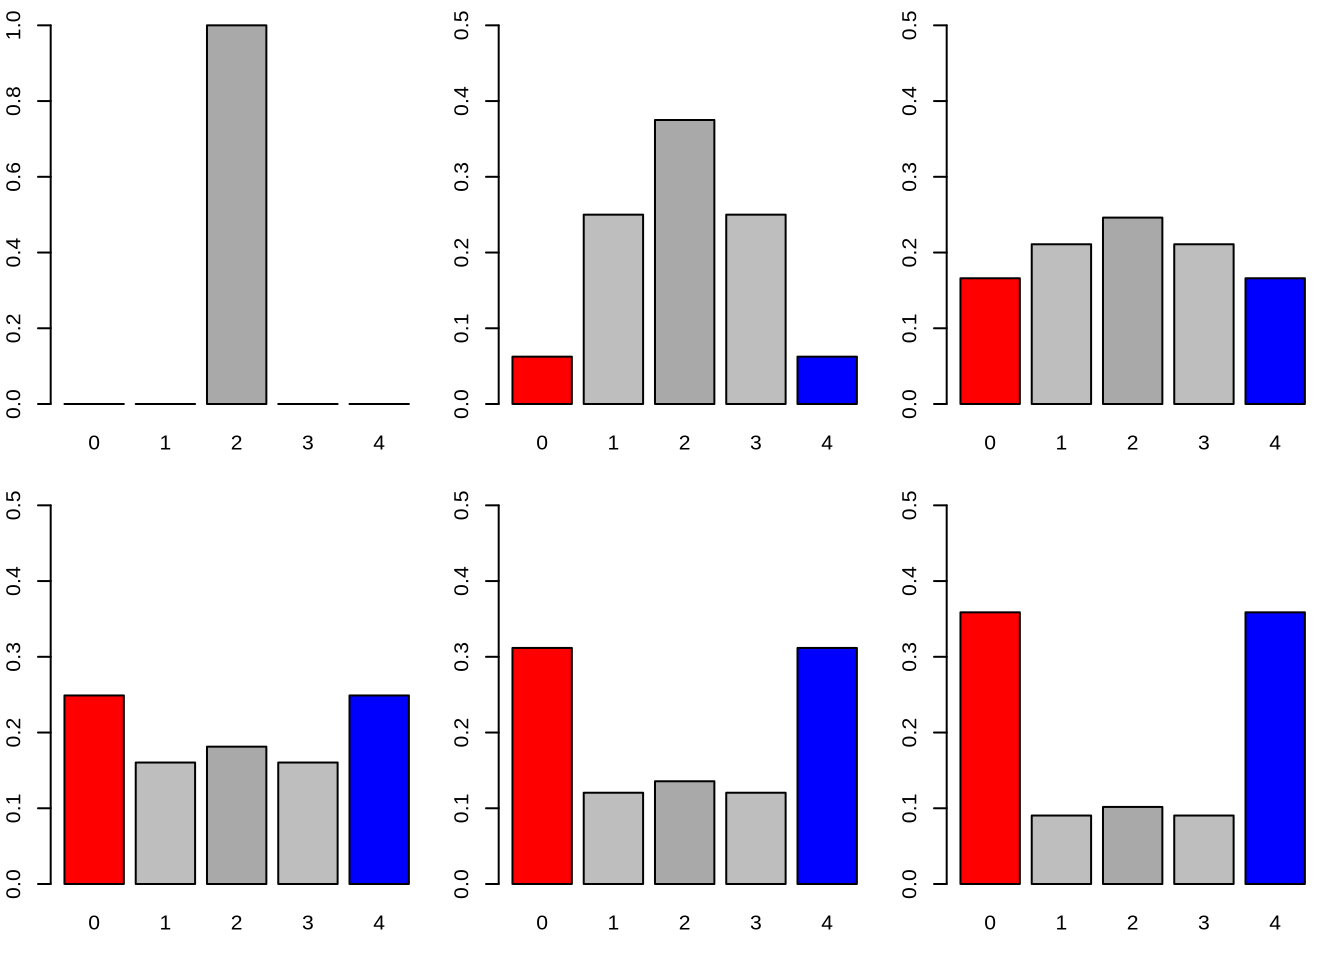
\includegraphics[width=0.8\linewidth]{ApuntesGeneticaII_files/figure-latex/figura3p6-1} 

}

\caption{Evolución de la probabilidad de encontrar a las poblaciones en un estado alélico determinado desde la generación $t=0$ a $t=5$ (desde el costado superior izquierdo al inferior derecho). En rojo el estado de 0 alelos A (pérdida del mismo), en azul 4 alelos A (fijación del mismo) y en gris oscuro 2 alelos (nuestro punto de partida en todas las poblaciones). Notar la diferente escala de la generación $t=0$ al resto.}\label{fig:figura3p6}
\end{figure}

Volvamos entonces a la pregunta anterior: ¿hacia dónde va el movimiento de las frecuencias en las distintas poblaciones a largo plazo? Para abordar esta cuestión, tendremos en cuenta el razonamiento de que \(\mathbf{I}_{t=k}=\mathbf{I}_0 * \mathbf{T}^{(k)}\). Resulta interesante ver cómo se comporta \(\mathbf{T}^{(k)}\) cuando \(k \to \infty\), es decir cuando el número de generaciones tiende a infinito. Una aproximación numérica sencilla consiste en elevar \(\mathbf{T}\) a un número suficientemente grande (\emph{e.g} 50 generaciones) y ver la forma que adquiere la matriz, como aparece en la Tabla \ref{tab:matrizMarkov50}.

\begin{table}
\centering
\caption{\label{tab:matrizMarkov50}Matriz de transición para un locus con dos alelos y dos individuos diploides luego de 50 generaciones.}
\centering
\begin{tabular}[t]{l|r|r|r|r|r}
\hline
  & a 0 alelos A & a 1 alelos A & a 2 alelos A & a 3 alelos A & a 4 alelos A\\
\hline
\cellcolor{gray!10}{de 0 alelos A} & \cellcolor{gray!10}{1,00} & \cellcolor{gray!10}{0} & \cellcolor{gray!10}{0} & \cellcolor{gray!10}{0} & \cellcolor{gray!10}{0,00}\\
\hline
de 1 alelos A & 0,75 & 0 & 0 & 0 & 0,25\\
\hline
\cellcolor{gray!10}{de 2 alelos A} & \cellcolor{gray!10}{0,50} & \cellcolor{gray!10}{0} & \cellcolor{gray!10}{0} & \cellcolor{gray!10}{0} & \cellcolor{gray!10}{0,50}\\
\hline
de 3 alelos A & 0,25 & 0 & 0 & 0 & 0,75\\
\hline
\cellcolor{gray!10}{de 4 alelos A} & \cellcolor{gray!10}{0,00} & \cellcolor{gray!10}{0} & \cellcolor{gray!10}{0} & \cellcolor{gray!10}{0} & \cellcolor{gray!10}{1,00}\\
\hline
\end{tabular}
\end{table}

Si miramos las columnas de la Tabla \ref{tab:matrizMarkov50} podemos apreciar dos situaciones claramente distintas; en las columnas 2, 3 y 4 (que corresponden a pasar de una generación a la siguiente a los estados de 1, 2 y 3 alelos \textbf{A} respectivamente), todas las celdas son 0, es decir más allá del punto de arranque (el vector de frecuencias o probabilidades \(\mathbf{I}_0\)), cuando el tiempo tiende a infinito (en principio lo estaríamos viendo con solo 50 generaciones) estos estados alélicos estarán vacíos (ninguna población tendrá 1, 2 o 3 alelos \textbf{A}), en nuestro modelo de dos individuos diploides. En cambio, las columnas 1 y 5, que se corresponden a la fijación del alelo \textbf{a} (pérdida del alelo \textbf{A}) y la fijación del alelo \textbf{A} respectivamente plantean una distribución que parece en espejo una de otra; claramente estas columnas se corresponden a las dos \textbf{barreras absorbentes}. Si nos fijamos en la columna 1, el único 0 corresponde a la probabilidad de pasar de 4 alelos \textbf{A} a 0 alelos \textbf{A}. Esto es trivial, ya que si el alelo \textbf{A} se encuentra fijado, al no existir mutación es imposible que las poblaciones evolucionen a otro estado alélico. Inversamente, en la columna 5 el único 0 se corresponde a la probabilidad de pasar de 0 a 4 alelos \textbf{A}. Esto también trivial, ya que no existe posibilidad de pasar del alelo \textbf{a} fijado a otro estado alélico. El resto de las celdas es fácil de explicar, si recordamos las probabilidades de fijación de un alelo dada su frecuencia inicial en la población. Cuando se parte de 1 solo alelo \textbf{A} (\emph{i.e.}, 3 alelos \textbf{a}), la probabilidad de fijación del alelo \textbf{a} es \(\frac{3}{4}\); cuando se parte de 2 alelos \textbf{A}, es de \(\frac{2}{4}=\frac{1}{2}\), y cuando se parte de 3 alelos \textbf{A} (\emph{i.e.} solo 1 alelo \textbf{a}), la probabilidad de fijación del alelo \textbf{a} es \(\frac{1}{4}\). Lo mismo acontece de forma inversa para las transiciones representadas en la columna 5.

La conclusión de todo lo anterior no es menor: con la matriz de probabilidad de transiciones \(\mathbf{T}\) (\ref{tab:matrizMarkov}) el estado estacionario (cuando \(t \to \infty\)) implica que \textbf{solo los estados de fijación de alguno de los alelos tienen probabilidad mayor a cero}. El punto de partida solo influirá en la distribución entre ellos, pero no en que solo ellos pueden tener probabilidad positiva de fijación. Pongamos un ejemplo: todas las poblaciones inicialmente tienen 1 alelo \textbf{A} de los 4 posibles (recordar que son dos individuos diploides, \(2N=4\)), es decir, \(\mathbf{I}_0=(0;1;0;0;0)\). Si multiplicamos este vector inicial de probabilidades (probabilidades de encontrar poblaciones del \textbf{ensemble} en ese estado), tenemos que \(\mathbf{I}_0*\mathbf{T}^\infty\) (llamamos \(\mathbf{T}^\infty\) a la potencia infinita, aunque en este contexto \(\mathbf{T}^{50} \sim \mathbf{T}^\infty\)), el resultado es \(\mathbf{I}_0*\mathbf{T}^\infty=(0,75;0;0;0;0,25)\), claramente en línea con lo que esperábamos: ninguna población aún segregando (1, 2 o 3 alelos \textbf{A}), \(75\%\) de la poblaciones con el alelo \textbf{a} fijado y \(25\%\) de las poblaciones con el alelo \textbf{A} fijado.

Si en lugar de haber arrancado con todas las poblaciones con 1 solo alelo \textbf{A}, hubiésemos arrancado con \(25\%\) de las poblaciones con 1 alelo \textbf{A}, \(25\%\) con dos alelos y \(50\%\) con 3 alelos \textbf{A}, entonces \(\mathbf{I}_0=(0;0,25;0,25;0,50;0)\). Por lo tanto \(\mathbf{I}_0*\mathbf{T}^\infty=(0,4375;0;0;0;0,5625)\), es decir que el \(43,75\%\) de las poblaciones de nuestro \textbf{ensemble} tendrían fijado el alelo \textbf{a} y el restante \(56,25\%\) tendría fijado el alelo \textbf{A}.

En general, si la deriva genética es la única fuerza evolutiva actuante (sin selección, sin mutación, sin migración), el equilibrio se alcanza cuando más tarde o más temprano todas las poblaciones se encuentran fijadas para uno de los dos alelos.

Un último punto que cabe mencionar acá. Si observamos la forma en la que crece la suma de los estados correspondientes a las \textbf{barreras absorbentes}, es posible demostrar que a partir de determinado punto la tasa de aproximación al estado de equilibrio es igual a \((1-\frac{1}{2N})\). Dicho de otra forma, a partir de determinado momento, a cada generación la proporción de poblaciones aún segregantes se reduce en \(\frac{1}{2N_e}\), proporción que va a parar de los estados correspondientes a las \textbf{barreras absorbentes}.

\section{Tamaño efectivo poblacional}\label{tamauxf1o-efectivo-poblacional}

Un punto que mencionamos antes pero no abundamos fue la diferencia entre el tamaño censal de una población, es decir el número \(N\) de individuos que la conforman y el tamaño efectivo de la misma, que llamamos \(N_e\). A veces resulta claro cuando en determinadas estructuras poblacionales particulares no tiene ningún sentido el número \(N\) como un indicador del comportamiento genético de la población, por ejemplo cuando un solo macho es responsable de todas las crías, pero otras veces no resulta tan claro. En todo caso, dada la dependencia de varias de nuestras ecuaciones de algún número que represente el tamaño poblacional, es necesario definir qué significa ese número a la luz de las cosas que hemos asumido en nuestros modelos.

Un ejemplo claro lo representa el supuesto de tamaño poblacional constante que hemos usado en el modelo de Wright-Fisher. Desafortunadamente, este supuesto es difícil de constatar en la realidad ya que las poblaciones fluctúan de tamaño, algunas en forma de tendencia (al crecimiento o decrecimiento) y otras a través de ciclos (por ejemplo, tamaños poblacionales de presa y predador, que están íntimamente relacionados). En este sentido, podríamos pensar en obtener un número poblacional en una población \textbf{perfecta} (para nuestro modelo) en la que de alguna manera el efecto genético de la deriva fuese equivalente al de nuestra población real. Si el tamaño poblacional fluctúa en el tiempo, podríamos por ejemplo pensar en que la media aritmética (el clásico promedio, que conoces muy bien) del tamaño censal sería un buen resumen del impacto genético de la deriva en la población. Desafortunadamente, el impacto genético de los tamaños poblacionales pequeños es desproporcionadamente alto, como puede verse en la Figura \ref{fig:figura3p8}.

\begin{figure}[H]

{\centering 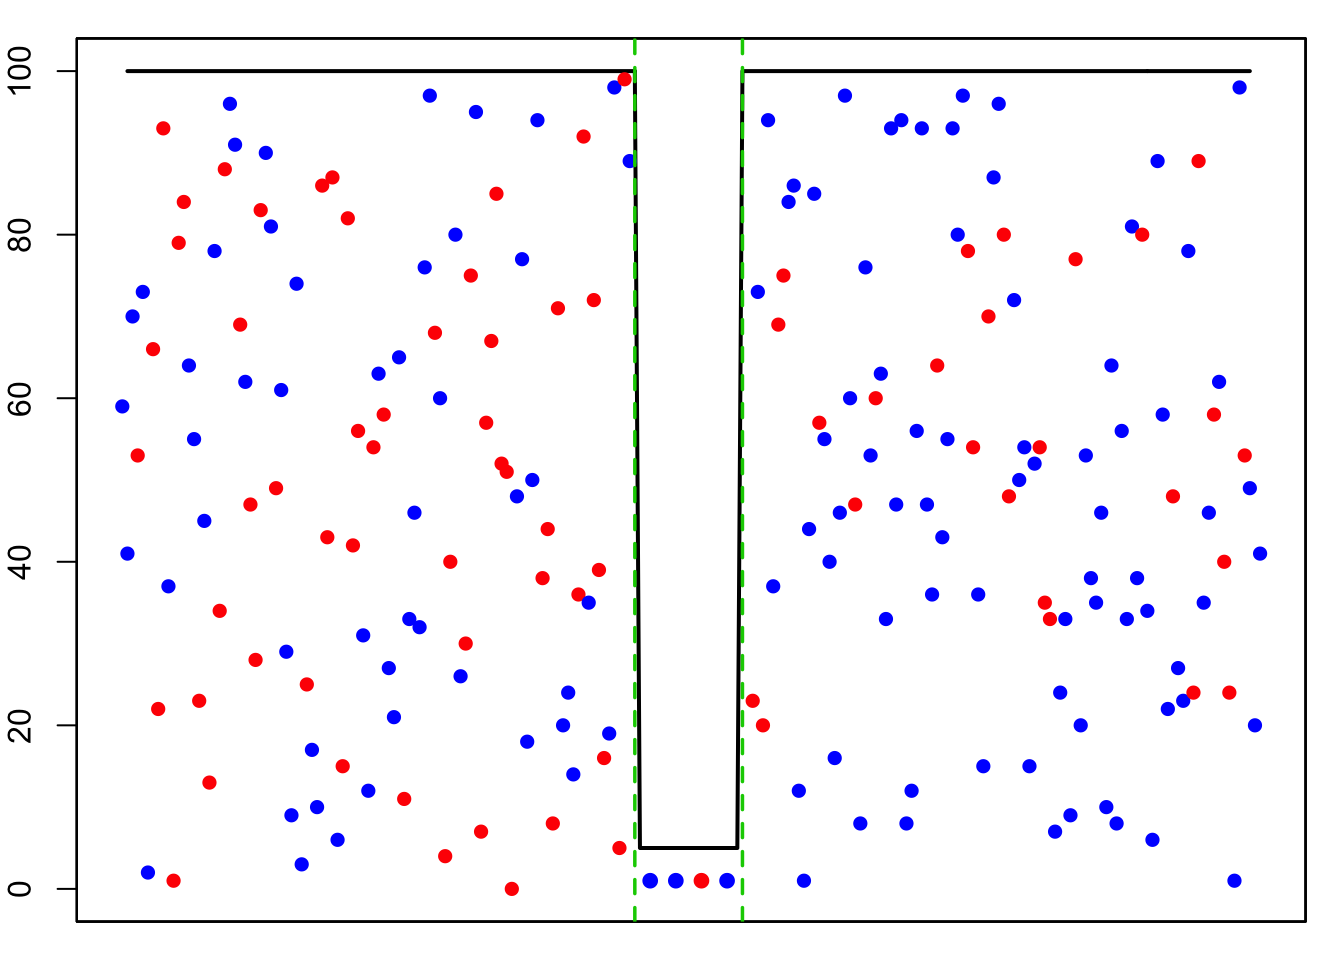
\includegraphics[width=0.8\linewidth]{ApuntesGeneticaII_files/figure-latex/figura3p8-1} 

}

\caption{Efecto de un cuello de botella poblacional en la frecuencia alélica. La población de 100 alelos, 50 rojos y 50 azules, se ve drásticamente reducida en una generación a 4 alelos (entre las dos líneas verdes), que por muestreo aleatorio son ahora 3 azules y 1 rojo. Luego de ese cuello de botella la población vuelve a expandirse al nivel inicial, pero la frecuencia ya quedó alterada en forma importante (figura propia sobre idea de @Hamilton2009).}\label{fig:figura3p8}
\end{figure}

En efecto, pese a que la población inicial era de 50 individuos diploides, o sea 100 alelos, 50 rojos y 50 azules, al sufrir un cuello de botella poblacional (sobreviven 2 individuos diploides, marcado por las dos líneas verdes en la Figura \ref{fig:figura3p8}) se muestrean 3 alelos azules y 1 rojo (un evento que tiene una probabilidad de \(\frac{1}{4}=25\%\)). Al expandirse nuevamente la población a 50 individuos, es decir 100 alelos, lo hará desde la frecuencia del cuello de botella. Resulta clara la influencia desproporcionada (respecto a un promedio simple) que tiene el muestreo durante el cuello de botella poblacional.

Veamos entonces una forma más razonable de estimar el tamaño de una población que fluctúa en número. Para hacer nuestro razonamiento supongamos que la población va de la generación 0 hasta la 2. De acuerdo a lo que vimos en la sección de \hyperref[homocigosidad-y-heterocigosidad]{Homocigosidad y Heterocigosidad},

\begin{equation}
1-F_2=\left(1-\frac{1}{2N_1}\right)(1-F_1)
\label{eq:F1}
\end{equation}

\begin{equation}
1-F_1=\left(1-\frac{1}{2N_0}\right)(1-F_0)
\label{eq:F2}
\end{equation}

Sustituyendo \eqref{eq:F2} en \eqref{eq:F1}, tenemos:

\begin{equation}
1-F_2=\left(1-\frac{1}{2N_1}\right)\left(1-\frac{1}{2N_0}\right)(1-F_0)
\label{eq:F3}
\end{equation}

Si el tamaño \(N\) fuese constante, obtendríamos el \(N_e\) generalizando esta expresión para un tiempo \(t\)

\begin{equation}
1-F_t = (1-\frac{1}{2N_e})^{t}(1-F_0)
\label{eq:F4}
\end{equation}

Por ejemplo, en el caso en que \(t=2\), la ecuación \eqref{eq:F4} se transforma en

\begin{equation}
1-F_2=(1-\frac{1}{2N_e})^2 (1-F_0)
\label{eq:F5}
\end{equation}

Ahora, si igualamos el resultado ``real'' (ecuación \eqref{eq:F3}) a la ``ideal'' (ecuación \eqref{eq:F5}), tenemos:

\begin{equation}
\begin{split}
1-F_2=(1-\frac{1}{2N_e})^2(1-F_0)=(1-\frac{1}{2N_1})(1-\frac{1}{2N_0})(1-F_0)=1-F_2
(1-\frac{1}{2N_e})^2=(1-\frac{1}{2N_1})(1-\frac{1}{2N_0})
\end{split}
\label{eq:F6}
\end{equation}

Desarrollando la ecuación \eqref{eq:F6}, tenemos que:

\begin{equation}
\begin{split}
1-2\frac{1}{2N_e}+\frac{1}{4N_e^2}=1-\frac{1}{2N_0}-\frac{1}{2N_1}+\frac{1}{4N_0N_1}
\frac{1}{N_e}-\frac{1}{4N_e^2}=\frac{1}{2}\left(\frac{1}{N_0}+\frac{1}{N_1}\right)-\frac{1}{4N_0N_1}
\end{split}
\label{eq:F7}
\end{equation}

y considerando que los términos en \(\frac{1}{4N_e^2}\) y \(\frac{1}{4N_0N_1}\) no afectan casi el resultado, porque su orden es casi similar, llegamos a que:

\begin{equation}
\frac{1}{N_e}=\frac{1}{2}(\frac{1}{N_0}+\frac{1}{N_1})
\label{eq:F7}
\end{equation}

es una muy buena aproximación. De hecho, esto significa que \(N_e\) es la \textbf{media armónica} entre \(N_0\) y \(N_1\). En general, para \(t \ge 2\) la media armónica (el recíproco de la media de recíprocos) es un buen indicador del \textbf{tamaño efectivo poblacional}:

\begin{equation}
\frac{1}{N_e}=\frac{1}{t}\left(\frac{1}{N_0}+\frac{1}{N_1}+\frac{1}{N_2}+...+\frac{1}{N_{t-1}} \right)
\end{equation}

\begin{equationbox}
\begin{equation}
N_e=\frac{t}{\left(\frac{1}{N_0}+\frac{1}{N_1}+\frac{1}{N_2}+...+\frac{1}{N_{t-1}} \right)}
\label{eq:Ne1}
\end{equation}

\end{equationbox}

\subsection*{Ejemplo 3.3}\label{ejemplo-3.3}
\addcontentsline{toc}{subsection}{Ejemplo 3.3}

El venado de campo (\emph{O. bezoarticus}) fue una especie típica de nuestro país (``\emph{extremadamente abundante}'' en palabras de Charles Darwin, que al pasar por estas tierras no dudó en llevarse ejemplares en el Beagle).
Lamentablemente, la población ha sufrido una disminución importante durante el último siglo.
Imaginemos que en un momento una población estaba compuesta por \(50000\) individuos, y que en la actualidad se compone por \(1000\) individuos.
Si en un esfuerzo descomunal se lograra recuperar el tamaño de la población, ¿cuál sería su tamaño poblacional efectivo, considerando que pasó por dicho cuello de botella?

El tamaño poblacional efectivo (\(N_e\)) se calcula a partir de la media armónica de los tamaños poblacionales mencionados:

\[
\frac{1}{N_e} = \frac{1}{3}(\frac{1}{50000} + \frac{1}{1000} + \frac{1}{50000}) \Rightarrow
\]

\[
N_e = \frac{3}{(\frac{1}{50000} + \frac{1}{1000} + \frac{1}{50000})}
\]

lo cual da una estimación de

\[
N_e \approx 2885
\]

\begin{center}\rule{0.5\linewidth}{0.5pt}\end{center}

Otra fuente importante de diferencias entre el tamaño censal y el tamaño efectivo de una población es el desequilibrio entre el número de machos y el número de hembras, como veremos en detalle en otros capítulos. En general, si una población está constituida por \(N_m\) machos y \(N_h\) hembras, el número total de animales (individuos) es \(N_a=N_m+N_h\), mientras que (como deduciremos en otro capítulo), para una generación determinada

\begin{equationbox}
\begin{equation}
N_e=\frac{4N_mN_h}{N_m+N_h}
\label{eq:Ne2}
\end{equation}

\end{equationbox}

Cuando el número de hembras es igual al número de machos (\(N_h=N_m=\frac{N}{2}\)), algo bastante raro en las poblaciones comerciales (al menos de mamíferos), tenemos que para la misma generación la ecuación \eqref{eq:Ne2} se transforma en

\[
\begin{split}
N_e=\frac{4N_mN_h}{N_m+N_h}=\frac{4\frac{N}{2}\frac{N}{2}}{\frac{N}{2}+\frac{N}{2}}=\frac{N^2}{N}=N
\end{split}
\label{eq:Ne3}
\]

Es decir, \(N_e=N\), el tamaño efectivo poblacional es igual al tamaño censal.

\subsection*{Ejemplo 3.4}\label{ejemplo-3.4}
\addcontentsline{toc}{subsection}{Ejemplo 3.4}

El león marino (\emph{Otaria flavescens}) se reproduce de forma estacional, siguiendo una estructura de harén: un macho alfa territorial monopoliza la reproducción, apareándose con varias hembras.
Grandi et \emph{al.} (\citeproc{ref-Grandi2012}{Grandi et al. 2012}) realizaron censos en colonias de \emph{O. flavescens} en el norte de la Patagonia, contando el número de machos alfa y de hembras sexualmente activas.
En el año 2012, el censo de 33 colonias arrojó un conteo de 2534 machos alfa y 12097 hembras sexualmente activas.
¿Cual es el tamaño efectivo poblacional en este caso?

Si se asume que a lo largo de las estaciones existe un apareamiento aproximadamente al azar entre machos alfa y hembras sexualmente activas, se puede estimar el tamaño poblacional efectivo teniendo en cuenta el desbalance de sexos según

\[
N_e = \frac{4N_hN_m}{N_h + N_m}
\]

\[
N_e = \frac{4 \cdot 12097 \cdot 2534}{12097 + 2534} \Rightarrow N_e = 8381
\]

\begin{center}\rule{0.5\linewidth}{0.5pt}\end{center}

Finalmente, otra versión del tamaño efectivo poblacional es la que sale de nuestra definición del modelo ideal y de cuanto esperamos que sea su varianza. Si llamamos \(\Delta p=p_t-p_{t-1}\), es decir a la diferencia entre la frecuencia promedio en la generación \(t\) y la generación anterior (\(t-1\)), entonces la varianza de \(\Delta p\) estará dada por

\begin{equation}
Var(\Delta p)=\frac{p_{t-1}q_{t-1}}{2N}
\end{equation}

cuando el proceso cumple con todos los requerimientos del modelo de Wright-Fisher. Pero esto mismo podemos usarlo para estimar cuál sería el tamaño efectivo poblacional que generaría la misma varianza empírica que tenemos en \(\Delta p\), \(N_e^v\). Es decir, despejando \(N\), que ahora llamaremos \(N_e^v\), que es nuestra incógnita asumiendo que proviene de un proceso perfecto Wright-Fisher, tenemos

\begin{equationbox}
\begin{equation}
N_e^v=\frac{pq}{2 Var(\Delta p)}
\end{equation}

\end{equationbox}

En resumen, en esta última forma de calcular el tamaño efectivo poblacional hemos asumido que la varianza entre generaciones en la media de frecuencias alélicas proviene de un proceso de Wright-Fisher y esto nos permite estimar cuál sería el tamaño de las poblaciones que se corresponden con esa varianza.

\begin{graybox}

\begin{itemize}
\tightlist
\item
  El tamaño efectivo de una población (\(N_e\)) raramente coincide con el tamaño censal de la misma (\(N\)), siendo las razones para esto diversas (variación del tamaño en el tiempo, diferente número de machos que de hembras, diferencias muy importantes en el número de descendientes entre reproductores candidatos, etc.).
\item
  El efecto conocido como \textbf{cuello de botella} (\textbf{bottleneck}) poblacional se refiere a la \textbf{reducción drástica} del número de reproductores en algún momento de la vida de una población determinada y aunque luego la misma experimente una nueva expansión, el cuello de botella dejará huellas indelebles a nivel de la variabilidad genómica.
\item
  El tamaño efectivo poblacional cuando varía el tamaño de la población en el tiempo se puede calcular como la media armónica entre los tamaños a cada generación:
\end{itemize}

\begin{equation*}
N_e=\frac{t}{\left(\frac{1}{N_0}+\frac{1}{N_1}+\frac{1}{N_2}+...+\frac{1}{N_{t-1}} \right)}
\end{equation*}

\begin{itemize}
\tightlist
\item
  Cuando el número de reproductores machos es diferente del número de reproductores hembras, el tamaño efectivo de la población es inferior a la suma de individuos y lo podemos calcular como
\end{itemize}

\begin{equation*}
N_e=\frac{4N_mN_h}{N_m+N_h}
\end{equation*}

\begin{itemize}
\tightlist
\item
  Si asumimos que se trata de un proceso de Wright-Fisher perfecto, podemos obtener un estimado del tamaño efectivo poblacional que se corresponde con la varianza en la media de frecuencias alélicas entre generaciones a partir de la dicha varianza \textbf{observada} mediante
\end{itemize}

\begin{equation*}
N_e^v=\frac{pq}{2 Var(\Delta p)}
\end{equation*}

\end{graybox}

\section{Aproximación de difusión}\label{aproximaciuxf3n-de-difusiuxf3n}


\includegraphics[width=0.13\textwidth,height=\textheight]{figuras/topicoav.png}

\begin{recuadro}
Gran parte de los desarrollos de esta sección siguen directamente el libro Hartl and Clark (\citeproc{ref-HartlClark2007}{2007}), que entendemos es de los más claros al nivel del presente curso, mientras que otros siguen el libro de Walsh and Lynch (\citeproc{ref-WalshLynch2018}{2018}) que posee un apéndice dedicado al tema. Otras fuentes importantes son el libro de Denny and Gaines (\citeproc{ref-DennyGaines2000}{2000}) para los procesos de difusión en biología y el libro de Hamilton (\citeproc{ref-Hamilton2009}{2009}), que seguimos directamente también (más allá de modificaciones mínimas) y que trata con cierto detalle pero a un nivel muy razonable la aproximación por difusión en genética (que a su vez sigue el de Denny and Gaines (\citeproc{ref-DennyGaines2000}{2000})).

Inevitablemente, esta sección es bastante técnica y usaremos cálculo diferencial e integral en múltiples variables, así como algunos conceptos básicos de ecuaciones diferenciales en derivadas parciales. Si te sientes un poco oxidado en estos temas, en el \hyperref[apuxe9ndice-b-cuxe1lculo-diferencial-e-integral]{Apéndice B: Cálculo diferencial e integral} podrás repasar los principales conceptos.

Dada la complejidad de esta sección, no pretendemos que seas capaz de reproducir o aún entender cada paso o derivación (aunque nos pondría muy contentos si así fuese). Si te resulta imposible entender no te desanimes ya que podrás seguir el resto del curso en forma independiente de las derivaciones de esta sección. La idea es que puedas entender de dónde surgen algunos resultados muy importantes que veremos en este y otros capítulos. Es muy importante para la mente científica conocer y entender el origen de resultados y fórmulas que utilizarás a lo largo de tu carrera, tanto como estudiante como profesional. \textbf{\emph{¡Ánimo!}}

\end{recuadro}

Como vimos más arriba (\hyperref[cadenas-de-markov]{Cadenas de Markov}), la evolución del número de copias de un alelo en poblaciones idénticas es un proceso estocástico discreto y la evolución de los estados puede seguirse a través de la multiplicación de la matriz de probabilidades de transición (cadenas de Markov). Sin embargo, esta aproximación suele ser dificultosa o imposible en la práctica para manejar modelos más complejos y una buena aproximación para comprender el comportamiento a largo plazo viene por el lado de los procesos de difusión. En efecto, si consideramos el tiempo como una variable continua, re-escalando el tiempo en generaciones que habíamos utilizado hasta ahora mediante la transformación \(\tau=\frac{t}{N}\) y escalando el número de copias del alelo \textbf{A} (\(i\)) de tal forma que \(x=\frac{i}{2N}\), cuando \(N \to \infty\) ambas variables pasan a ser continuas.

\subsection*{Caminatas al azar y procesos de difusión}\label{caminatas-al-azar-y-procesos-de-difusiuxf3n}
\addcontentsline{toc}{subsection}{Caminatas al azar y procesos de difusión}

En la sección \hyperref[el-modelo-de-wright-fisher]{El modelo de Wright-Fisher} vimos el comportamiento de la frecuencia alélica guiada solo por el proceso de deriva genética. Si observamos nuevamente el trazo dejado por cualquiera de las poblaciones no resulta difícil imaginarse el recorrido de alguien que (posiblemente borracho) a cada instante en el tiempo, decide a través del resultado de tirar una moneda si el siguiente paso es a la derecha o a la izquierda. Más aún, podemos pensar que esta persona se encuentra sobre una línea trazada en el piso y que arranca desde una determinada posición inicial decidiendo con la moneda hacia dónde dar el siguiente paso. Lo que nos interesa entonces es estudiar el comportamiento de este tipo de procesos y ver si podemos hacer algunas predicciones al respecto. Más divertido aún y más cercano a lo que vamos a describir ahora sería un experimento donde a la salida de un bar (en un lugar medio desierto) reclutamos a todos los borrachos disponibles, los ponemos en ``fila india'' y les explicamos que al sonido de la campana (que tañeremos en forma regular) deben tirar una moneda y en función del resultado dar un paso a la derecha (si sale cara) o a la izquierda (si sale cruz); o aún quedarse quietos si no sintieron la campana o estaban distraídos. Bueno, también se podría hacer sin borrachos, pero intuimos que será mucho más divertido en el primer caso.

En realidad, existe una motivación física mucho más potente y que usaremos como analogía para luego pasar a ver cómo esa analogía nos puede ayudar a entender los procesos estocásticos en las frecuencias alélicas de nuestras poblaciones. La motivación es muy sencilla: imaginemos que en el instante \(t=0\) dejamos caer una gota de tinta en la posición central de un canal horizontal abierto conteniendo agua (el canal se extiende a derecha, signo positivo, e izquierda, signo negativo, de \(x=0\)). En ambos extremos del canal tenemos un medio que absorbe las partículas de tinta a medida de que van arribando (es decir, son \textbf{barreras absorbentes} para las partículas de tinta). El papel de nuestros ``borrachos'' lo representarán ahora las pequeñas partículas de tinta que formaban la gota y que ahora, a partir del instante \(t=0\) comenzarán a dispersarse en ambas direcciones. Para que nuestra analogía tenga cierto sentido físico y poder estudiar su comportamiento vamos a definir una serie de reglas que se aplican al movimiento individual de cada partícula.

\begin{recuadro}

\textbf{Reglas}

\begin{enumerate}
\def\labelenumi{\arabic{enumi}.}
\item
  La partícula comienza en la posición \(x=0\) en el instante inicial, \(t=0\).
\item
  La partícula se mueve \textbf{una distancia fija} \(\delta\) en cada intervalo de tiempo \(\tau\).
\item
  La partícula se puede mover solo en el eje permitido, con probabilidad \(p=\frac{1}{2}\) hacia la derecha (arbitrariamente, puede ser cualquier dirección) y por lo tanto con probabilidad \(q=1-p=1-\frac{1}{2}=\frac{1}{2}\) hacia la izquierda (o en sentido opuesto al anterior).
\item
  El sentido en el que se mueve es independiente del sentido en la movida anterior, o lo que es lo mismo, se trata de un proceso \textbf{sin memoria} (recordar lo visto en la sección \hyperref[cadenas-de-markov]{Cadenas de Markov}).
\item
  Pueden existir tantas partículas como se quiera en la misma posición del eje sin interferir unas con otras (es como si cada una ``corriese'' por su propio carril, todos los carriles paralelos unos a otros).
\end{enumerate}

\end{recuadro}

En la Figura \ref{fig:difusion} podemos ver una representación esquemática de nuestro diseño. En el instante \(t=0\) consideramos que cae la gota de tinta (roja) al agua \textbf{al mismo tiempo} que las \textbf{partículas} que la constituyen comienzan a difundir hacia izquierda y derecha de acuerdo a las reglas que establecimos más arriba.

\begin{figure}[H]

{\centering 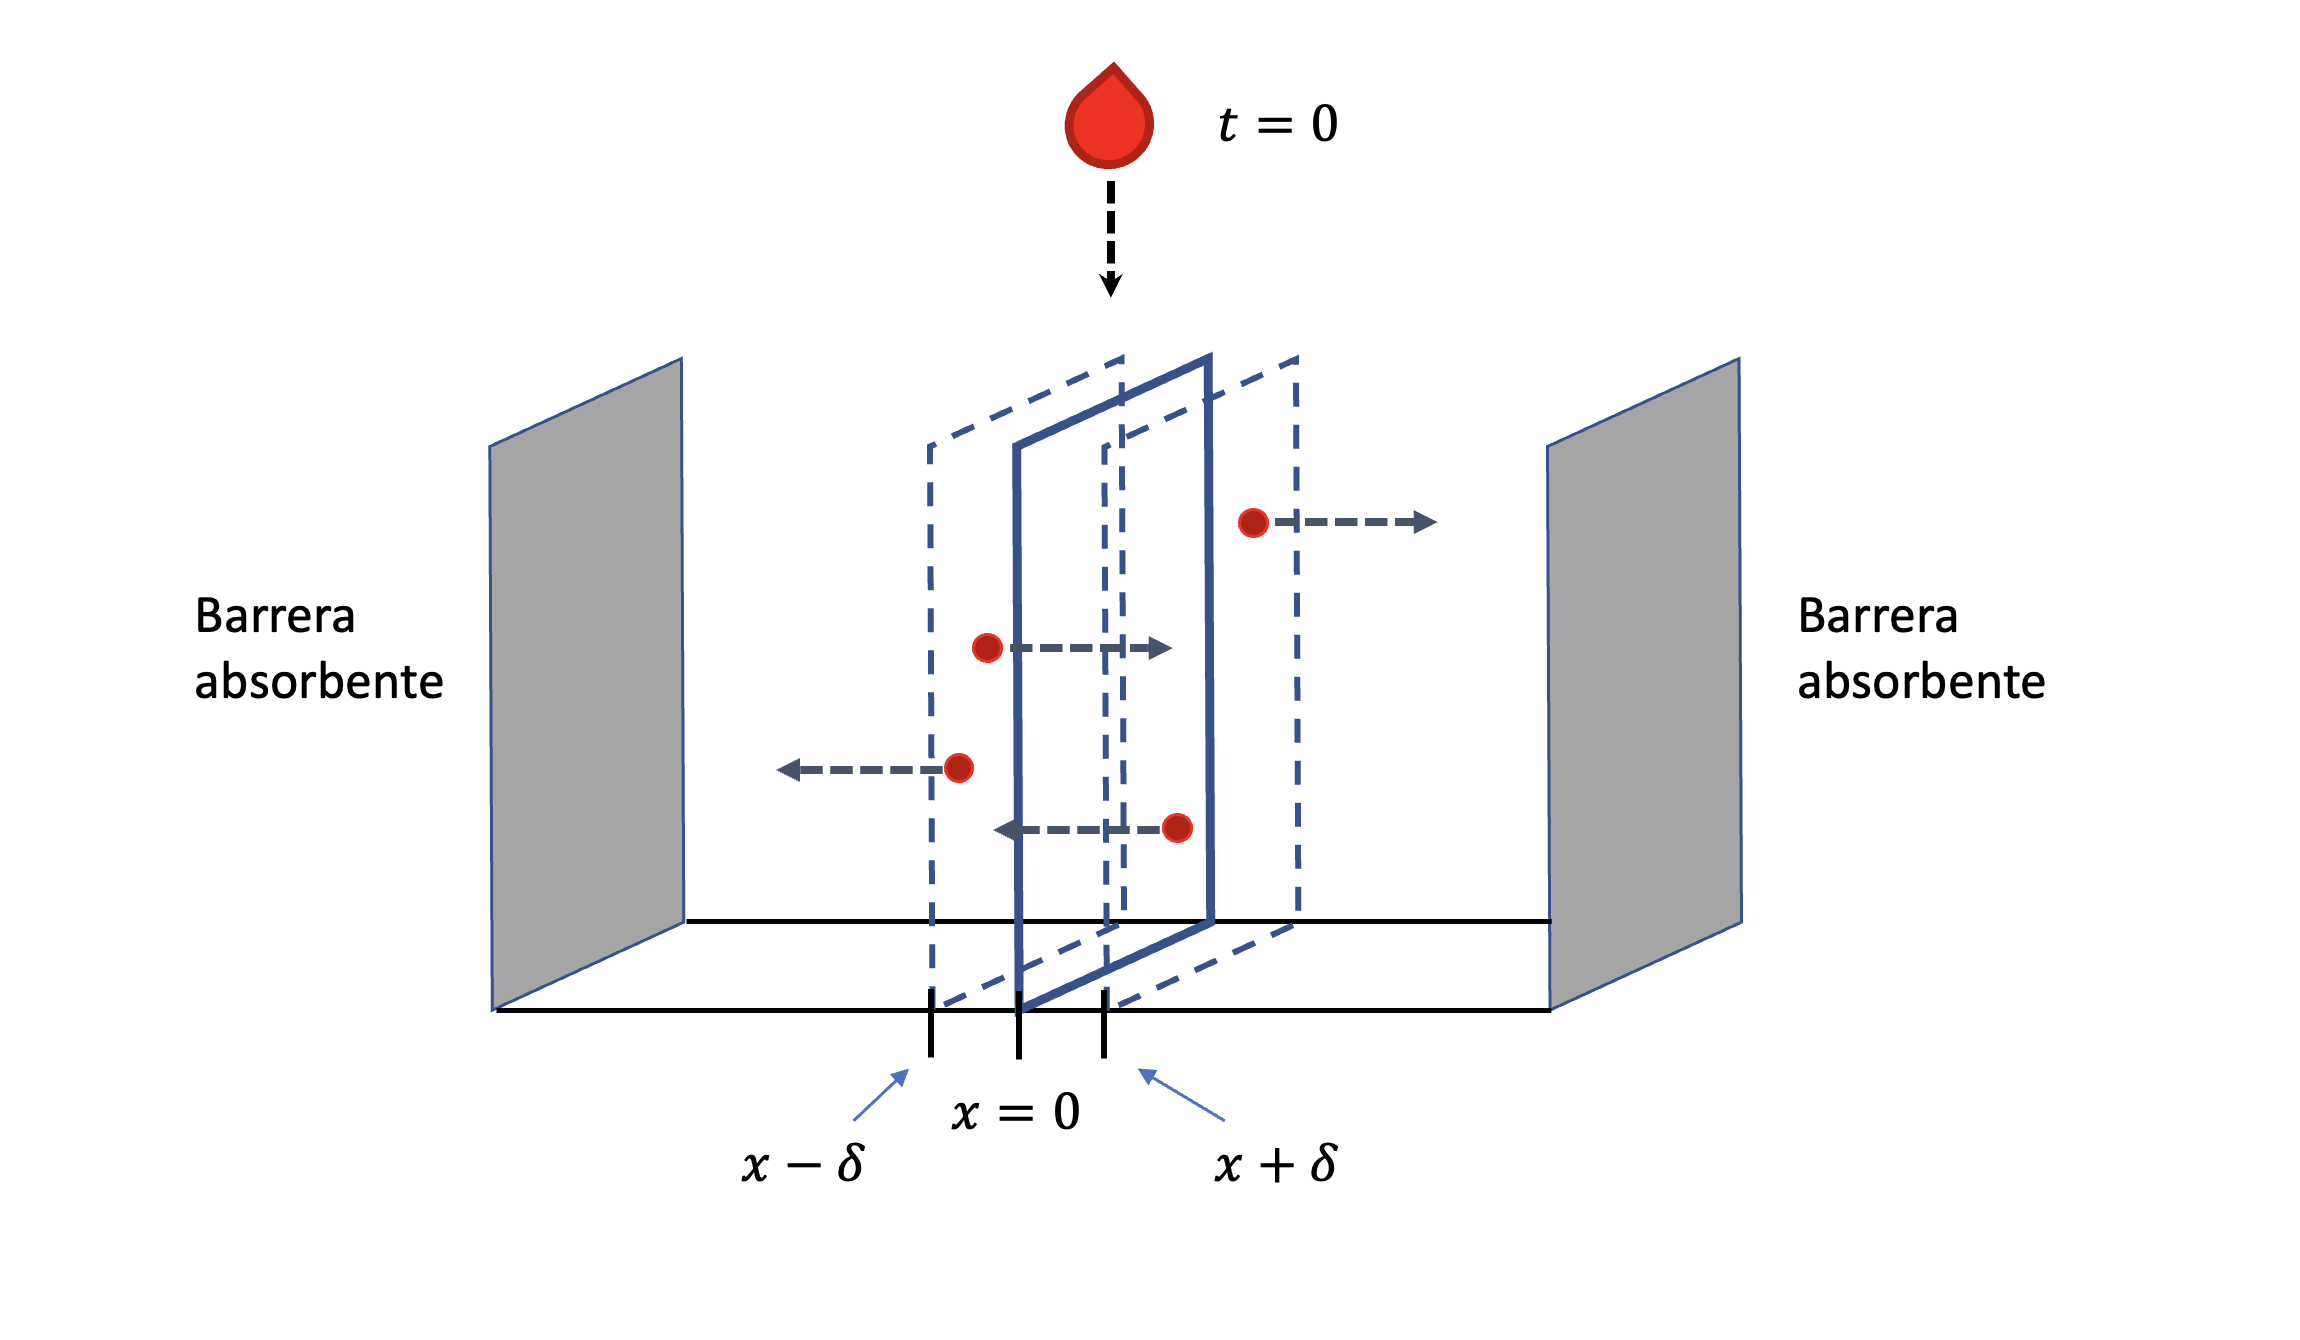
\includegraphics[width=0.8\linewidth]{figuras/difusion2} 

}

\caption{Diagrama que representa el escenario para el movimiento de nuestras partículas de tinta. En el instante inicial la gota de tinta cae  al mismo tiempo sus partículas constituyentes comienzan a difundir a izquierda y derecha (elaboración propia sobre idea de @Hamilton2009).}\label{fig:difusion}
\end{figure}

Primero, podríamos analizar qué ocurre con la posición promedio de las partículas a medida de que avanza el tiempo, por ejemplo en una unidad (\(\tau\)). La posición media está dada por

\begin{equation}
\bar{x}=p(\delta)+q(-\delta)
\end{equation}

Como las partículas se mueven a derecha e izquierda con la misma probabilidad, \(\delta\) y \(-\delta\) unidades de posición, entonces tenemos que luego de una unidad de tiempo \(\tau\) la posición media será en nuestro caso

\begin{equation}
\bar{x}=\frac{1}{2}(\delta)-\frac{1}{2}(\delta)=0
\label{eq:difu1}
\end{equation}

Es decir, que la posición media de las partículas será la misma que al comienzo. Esto no debería extrañarnos dado de que por simetría del problema tantas partículas se moverán hacia un lado como otras en el sentido opuesto, lo que da un balance neto de cero respecto al desplazamiento del punto medio. Entonces, ¿nada ha cambiado? Si recuerdas el comportamiento de las distintas poblaciones en la Figura \ref{fig:figura3p5}, posiblemente te habrás imaginado que si bien la media del proceso no cambia, la varianza sí lo hace. Si además recuerdas la fórmula para la varianza

\begin{equation}
Var(x)=E(x^2)-E^2(x)
\end{equation}

y que además en nuestro caso \(E^2(x)=E(x)E(x)=\bar{x}\bar{x}=0 \cdot 0\), llegaremos enseguida a la conclusión de que la varianza en posición de las partículas es igual a \(E(x^2)\), o lo que es lo mismo el promedio de las posiciones al cuadrado. Como además, en cada intervalo arbitrariamente pequeño de tiempo la partícula solo puede moverse \(\delta\) en uno de los sentidos, la ubicación de la partícula \(i\) en el tiempo 1 será igual a

\begin{equation}
x_{i,(t=1)}=x_{i,(t=0)}+\delta
\end{equation}

con \(\delta\) positivo o negativo. O sea, para obtener una expresión de la varianza en las posiciones de las partículas, luego de un intervalo arbitrariamente pequeño (de \(t=0\) a \(t=1\)) debemos comenzar por elevar al cuadrado esta expresión y luego promediar

\[
\begin{split}
x_{i,(t=1)}^2=(x_{i,(t=0)}+\delta)^2\\
x_{i,(t=1)}^2=x_{i,(t=0)}^2+2x_{i,(t=0)}\delta+\delta^2
\end{split}
\]

Por lo tanto, promediando el resultado anterior para las N partículas obtenemos

\begin{equation}
\sigma^2(x_{i,(t=1)})=\frac{1}{N} \sum_{i=1}^{N} (x_{i,(t=0)}^2+2x_{i,(t=0)}\delta+\delta^2)
\end{equation}

La expresión anterior se puede simplificar bastante. En primer lugar, por una razón de simetría, habrá tantas partículas que se muevan a la derecha como a la izquierda (recordar \(\bar{x}=0\), ecuación \eqref{eq:difu1}), por lo que el término del medio es igual a cero. Luego

\[
\begin{split}
\sigma^2(x_{i,(t=1)})=\frac{1}{N}\sum_{i=1}^{N} x_{i,(t=0)}^2 + \frac{1}{N}N\delta^2\\
\sigma^2(x_{i,(t=1)})=\overline{x^2}_{i,(t=0)}+\delta^2
\end{split}
\]

Ahora, suponiendo que a \(t=0\) todas las partículas salen de la posición cero, entonces el promedio del cuadrado de sus distancias será 0 también (\(\overline{x^2}_{i,(t=0)}=0\)), por lo que nos quedamos con \(\delta^2\), es decir el cuadrado del cambio en posición en un intervalo de tiempo, como el incremento en la varianza en un avance arbitrariamente pequeño del tiempo (de \(t=0\) a \(t=1\)). En un intervalo de tiempo de \(t\) unidades, por lo tanto, la varianza de la posición de las partículas será de \(t\delta^2\), o dicho de otra manera, la varianza en la posición de las partículas se incrementa en forma lineal con el tiempo. En el primer instante la varianza será \(1 \cdot\delta^2=\delta^2\), en el segundo instante será \(2\delta^2\), luego \(3\delta^2\), etc. La anterior es una observación más que razonable para describir el fenómeno de cómo una gota de tinta se dispersa en el agua a medida de que pasa el tiempo.

Si definimos el \textbf{coeficiente de difusión} de las partículas (\(D\)) como la velocidad con que la tinta se difunde en el agua, tenemos que

\begin{equation}
D=\frac{1}{2}\frac{d\sigma^2}{dt}
\label{eq:difu2}
\end{equation}

La ecuación anterior es fácil de entender, la varianza representa la dispersión de las partículas en un momento dado y por lo tanto su derivada primera respecto del tiempo es su velocidad. Pero la varianza representa dispersión a ambos lados del punto de inicio, por lo que solo la mitad de la misma corresponderá a la magnitud de la velocidad en un sentido (de lo contrario, la velocidad neta siempre sería cero). Como \(\sigma^2=t\delta^2\), entonces

\begin{equation}
D=\frac{1}{2}\frac{d\sigma^2}{dt}=\frac{1}{2}\frac{d(t\delta^2)}{dt}=\frac{\delta^2}{2}
\label{eq:difu2p1}
\end{equation}

Es decir, \(D=\frac{\delta^2}{2}\) es la velocidad de difusión de las partículas, o lo que es lo mismo, un medio del incremento en la varianza en una unidad de tiempo arbitrariamente pequeño.

Volvamos ahora a la genética. ¿Cómo se relaciona esto del proceso de difusión con nuestro tratamiento de la evolución estocástica de las frecuencias alélicas en las poblaciones? En principio es muy sencillo: si consideramos que cada población del \textbf{ensemble} es como una partícula en nuestro modelo de difusión, los ``movimientos'' que puede realizar nuestras poblaciones son en lugar del movimiento físico de las partículas, los cambios en frecuencia alélica en la población. O sea, si por ejemplo, partimos de \(p_A=0,5\), es equivalente como partir del punto medio en el modelo de difusión. Ahora las \textbf{barreras absorbentes} estarán en \(p_A=0\) y \(p_A=1\). Por otra parte, si recuerdas lo tratado en la sección \hyperref[el-modelo-de-wright-fisher]{El modelo de Wright-Fisher}, la \textbf{varianza por generación} (o lo que sería un intervalo arbitrariamente pequeño en la difusión) era \(\sigma^2(p)=\frac{pq}{2N}\) y la varianza a lo largo del tiempo, en la generación \(t\), por ejemplo igual a \(\sigma^2_t(p)=t\frac{pq}{2N}\) (ecuación \eqref{eq:varWF}, para simplificar la notación llamaremos \(\sigma^2\) a \(\sigma^2_t(p)\)), por lo que podemos hacer:

\begin{equation}
\frac{d\sigma^2}{dt}=\frac{d(t\frac{pq}{2N})}{dt}=\frac{pq}{2N}
\label{eq:difu3}
\end{equation}

Si recordamos de la ecuación \eqref{eq:difu2} que \(D=\frac{1}{2}\frac{d\sigma^2}{dt}\) y substituimos en ella el resultado de la ecuación \eqref{eq:difu3}, tenemos que el coeficiente de difusión \(D\) es ahora

\begin{equation}
D=\frac{1}{2}\frac{d\sigma^2}{dt}=\frac{1}{2}\frac{pq}{2N}=\frac{pq}{4N}=\frac{p-p^2}{4N}
\label{eq:difu4}
\end{equation}

Es decir, el coeficiente de difusión para las frecuencias alélicas de nuestras poblaciones es una función de la frecuencia de los alelos (\(p\) y \(q\)). El denominador de la ecuación \eqref{eq:difu4} no depende de las frecuencias ya que se trata de un número \(N\) positivo, multiplicado por una constante positiva (4). En cambio, el numerador depende de la frecuencia del alelo \textbf{A} (\(p\)): si recuerdas de la sección \hyperref[heterocigotas-freq-alelica]{H-W: la frecuencia de heterocigotas en función de la frecuencia alélica}, el producto \(p \cdot q\) tiene un máximo cuando \(p=q=\frac{1}{2}\). Es decir la velocidad de difusión (cambio de frecuencias alélicas) será máxima cerca de \(p=\frac{1}{2}\) y tenderá a cero a medida que \(p\) se acerque a las barreras absorbentes de \(0\) y \(1\). Dicho de otra manera, la velocidad de cambio en la frecuencia en cada población será máximo en el entorno de \(p=\frac{1}{2}\), llevando a las poblaciones hacia las regiones donde el coeficiente de difusión es menor, cerca de las barreras absorbentes, donde al ser menor el coeficiente de difusión permanecerá más tiempo. Por otra parte, el coeficiente de difusión también depende del tamaño poblacional efectivo: a mayor número de individuos en cada una de las poblaciones que constituyen el \textbf{ensemble}, menor será el coeficiente de difusión, o lo que es lo mismo menor la velocidad con que cambian las frecuencias de los alelos en cada población.

Procuraremos ahora calcular la probabilidad de que una población se encuentre en una región en particular en el intervalo de frecuencias, o en nuestra analogía de difusión la probabilidad de encontrar una partícula en una posición en particular del eje en que se mueven. Para eso necesitaremos calcular el flujo de partículas en la región de interés, o dicho de otra forma el número neto de partículas que atraviesan un área definida por intervalo de tiempo. Si consideramos un área \(A\) el flujo neto de partículas que atraviesa la misma hacia la derecha (arbitrariamente) es igual a la mitad del número de partículas que están a una distancia \(\delta\) a la izquierda de la misma (recuerda que en cada posición la mitad de las partículas tenderá a moverse a la izquierda y la otra mitad a la derecha), menos la mitad de la partículas que a una distancia \(\delta\) a la derecha del área de referencia (\(\delta\) porque es la distancia a la que se mueven en una unidad de tiempo). Es decir:

\begin{equation}
N_{neto}(Der)=\frac{1}{2}N(Izq)-\frac{1}{2}N(Der)=-\frac{1}{2}[N(Der)-N(Izq)]
\end{equation}

Pero el flujo es la cantidad de partículas que atraviesan un área en determinado tiempo, por lo que para obtener una expresión de éste en el punto \(x\), que llamaremos \(J_x\) debemos dividir por área y por tiempo:

\begin{equation}
J_x=-\frac{1}{2}\frac{[N(Der)-N(Izq)]}{At}
\end{equation}

Si multiplicamos esta última expresión por 1, bajo la forma de \(\frac{\delta^2}{\delta^2}\), para luego rearreglar los términos, la misma quedará:

\begin{equation}
J_x=-\frac{\delta^2}{2t}\frac{1}{\delta}\frac{[N(Der)-N(Izq)]}{A\delta}=-\frac{\delta^2}{2t}\frac{1}{\delta}\left[\frac{N(Der)}{A\delta}-\frac{N(Izq)}{A\delta}\right]
\label{eq:difu5}
\end{equation}

Si observamos los dos términos entre paréntesis rectos de la ecuación anterior, en ambos casos (\(\frac{N(Der)}{A\delta}\) y \(\frac{N(Izq)}{A\delta}\)) se trata de un número de partículas dividido entre el producto de un área (\(A\)) por una distancia (\(\delta\)), es decir dividido entre un volumen (recuerda de la escuela cómo calculábamos los volúmenes). Pero el número de partículas divido entre el volumen que ocupan las mismas es la concentración, por lo que podemos llamar \(C(Der)\) y \(C(Izq)\) a la concentración de partículas a derecha e izquierda de nuestra área. Además, previamente habíamos visto (ecuación \eqref{eq:difu2p1}) que \(\frac{\delta^2}{2}=D\), por lo que en una unidad de tiempo (\(t=1\)), substituyendo en \eqref{eq:difu5} tenemos:

\begin{equation}
J_x=-D\frac{C(Der)-C(Izq)}{\delta}
\label{eq:difu6}
\end{equation}

Si asumimos que las partículas se encuentran uniformemente distribuidas en el intervalo entre \(x\) y \(x+\delta\) su posición promedio será \(\frac{\delta}{2}\) (lo mismo para el otro lado, pero ahora será \(-\frac{\delta}{2}\)), que tomaremos como posición característica. Entonces \(C(Der)=C(x+\frac{\delta}{2})\) y \(C(Izq)=C(x-\frac{\delta}{2})\), por lo que la ecuación \eqref{eq:difu6} la podemos escribir como:

\begin{equation}
J_x=-D\frac{C(x+\frac{\delta}{2})-C(x-\frac{\delta}{2})}{\delta}
\label{eq:difu7}
\end{equation}

Si en esta última expresión hacemos el paso al límite cuando las distancias en \(x\) son infinitamente pequeñas), es decir cuando \(\delta \to 0\), tenemos que:

\begin{equation}
J_x=-D\frac{dC}{dx}
\label{eq:difu7}
\end{equation}

que se conoce como la \textbf{primer ecuación de difusión de Fick}. Nuevamente, esta ecuación parece sencilla de interpretar. El coeficiente de difusión es un número positivo que indica la velocidad de movimiento de las partículas en el medio. Por otro lado, \(\frac{dC}{dx}\) representa el gradiente de la concentración de partículas (en nuestro caso de poblaciones) y cuando su signo es positivo indica la dirección hacia la mayor concentración de partículas. Como acá el producto tiene un signo negativo, la ecuación nos indica que las partículas (poblaciones) se moverán en dirección a donde hay una menor concentración (recordar la analogía con la gota de tinta en agua; la tinta se moverá hacia donde hay menor concentración). Obviamente, en el equilibrio, para cada posición en el eje de movimiento (nuestras frecuencias alélicas) tantas partículas se moverán hacia un lado como hacia el otro.

Pasemos ahora a intentar entender como esto nos puede aportar a entender el comportamiento de las frecuencias alélicas en nuestro \textbf{ensemble}. Para esto, debemos recordar que estamos tratando con una aproximación continua (las frecuencias alélicas ya no las expresamos como el número de copias de un alelo sino como este número divido entre \(2N\)) y por lo tanto la probabilidad la vamos a sustituir por una \textbf{densidad de probabilidad}, que llamaremos \(\phi(p,x,t)\) (notar la dependencia del punto inicial de partida \(p\), o sea la frecuencia inicial del alelo \textbf{A}). Esta densidad de probabilidad es equivalente a la concentración de partículas. \(\phi(p,x,t)\) representa el balance neto entre las poblaciones que arriban a esa frecuencia alélica \(x\) y aquellas que se alejan de la misma; pero esto, en nuestro razonamiento previo es el \textbf{flujo neto} en el punto \(x\), es decir \(J_x\). De acuerdo a la \textbf{ecuación de continuidad}, ya que el material no se crea o destruye,

\[
\begin{split}
\frac{d\phi(p,x,t)}{dt}+\frac{dJ_{x,t}}{dx}=0\\
\frac{d\phi(p,x,t)}{dt}=-\frac{dJ_{x,t}}{dx}
\end{split}
\label{eq:difu8}
\]

Hasta ahora nos hemos manejado asumiendo que el movimiento de las frecuencias alélicas en las distintas poblaciones se debe exclusivamente al azar (por eso \textbf{random drift}), pero para hacer más general nuestra ecuación debemos entender que las frecuencias alélicas también pueden variar de forma sistemática, por ejemplo a través de la mutación (fuera del equilibrio mutacional) y selección. La analogía con las partículas de tinta sería a través de suponer que las mismas tienen determinada carga eléctrica y que entre las dos barreras absorbentes existe una diferencia de potencial que hará que las partículas se muevan sistemáticamente en una dirección (efecto superpuesto al aleatorio). Otra analogía para intentar entender esta lógica de efectos superpuestos se plantea en la Figura \ref{fig:bolitas-tuboviento}, en donde se observa el comportamiento de bolitas de diferente densidad al ingresar a un tubo de viento que cuenta a su vez con un sistema de ventilación interno.

\begin{figure}[H]

{\centering 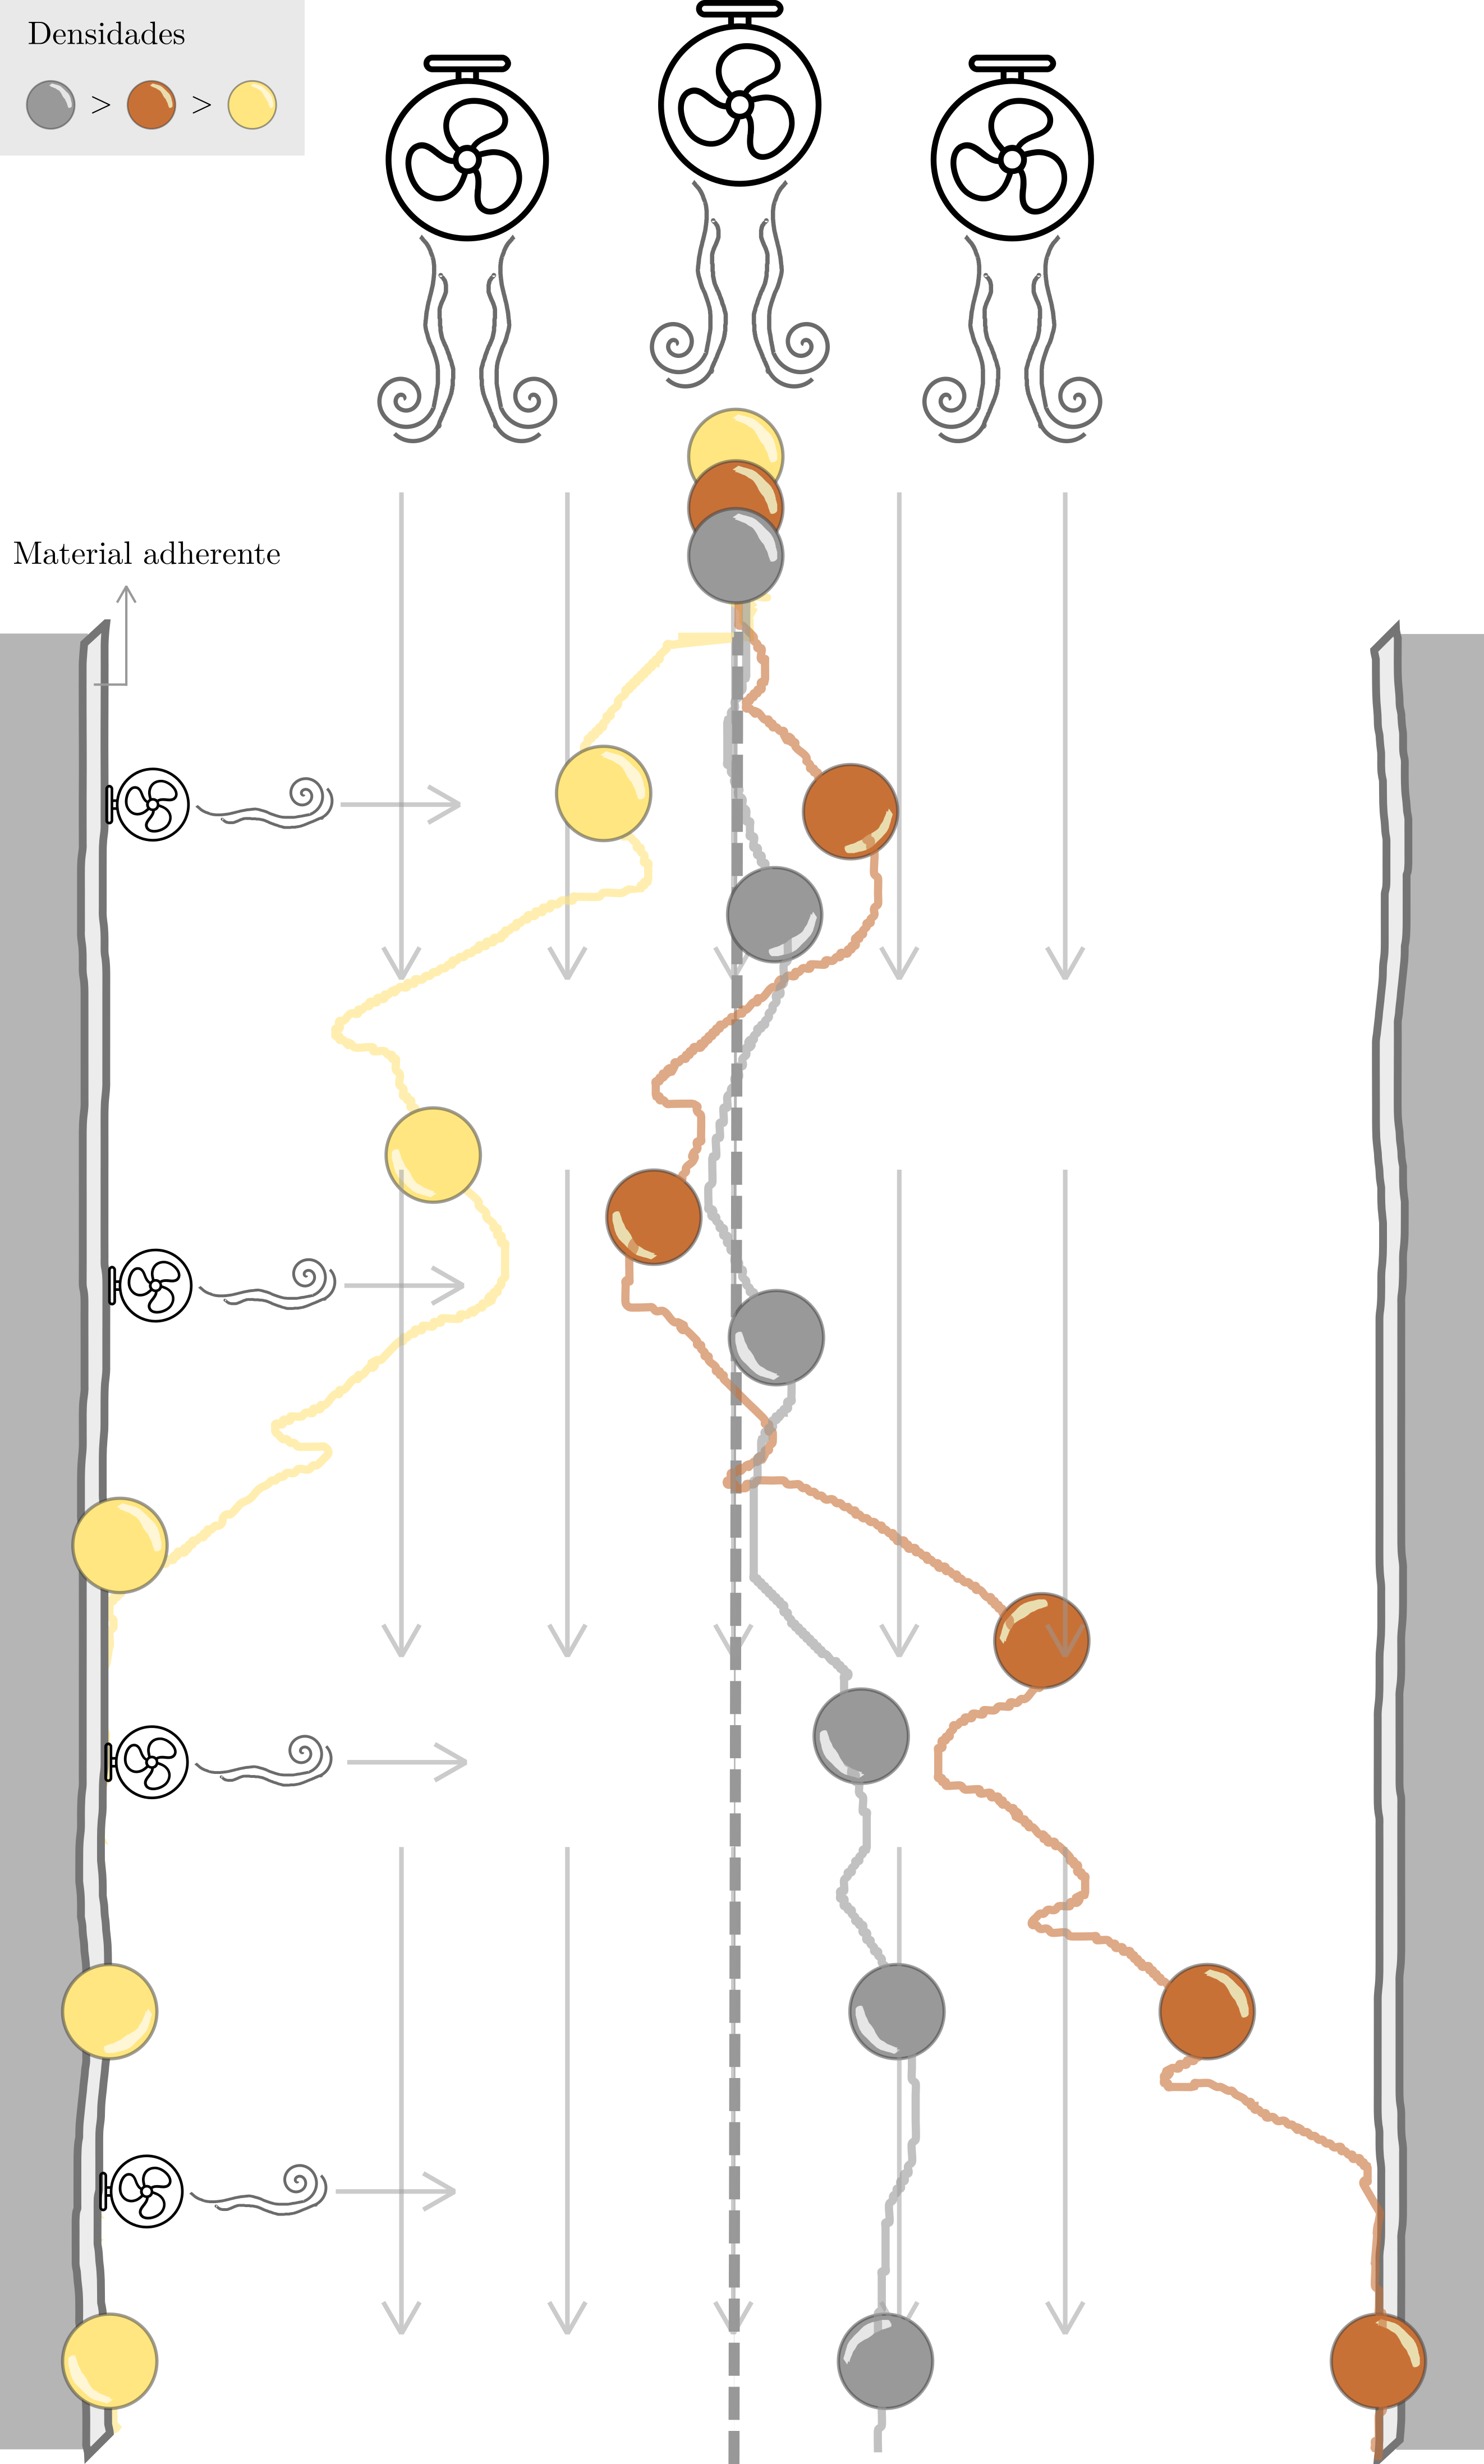
\includegraphics[width=0.5\linewidth]{figuras/bolitas_y_difusion} 

}

\caption{Diagrama que representa posibles trayectorias de bolitas de diferente densidad (\textit{e.g} una pelotita de ping-pong, una de madera y una de metal) al ingresar a un tubo de viento con un sistema de ventilación interno. El sistema cuenta a su vez con un material adherente sus costados, por lo que las bolitas que entren en contacto con el borde continuarán su trayectoria sobre él. Dos efectos superpuestos influyen sobre la trayectoria de cada bolita: a) el flujo de viento a través del tubo, generado por ventiladores superiores, y b) una corriente de menor intensidad, de izquierda a derecha, generada por un sistema de ventilación interno. El efecto del flujo de viento superior es aleatorio respecto al plano horizontal, pudiendo cada bolita desplazarse a cada lado con igual probabilidad debido a este estímulo. En cambio, el efecto de la ventilación interna es sistemático, favoreciendo un movimiento de izquierda a derecha en cada bolita. Según su densidad, cada bolita responderá a estos estímulos de manera diferente. Notemos como en el ejemplo la bolita de ping-pong se inclinó tempranamente hacia la izquierda, lo cual favoreció su contacto con dicho borde. Las otras bolitas (de mayor densidad), presentan menores varianzas respecto a su movimiento horizontal.}\label{fig:bolitas-tuboviento}
\end{figure}

Ahora, si llamamos \(M(x)\) a ese efecto sistemático, tenemos entonces

\begin{equation}
J_{x,t}=M(x)\phi(p,x,t)-D\frac{d\phi(p,x,t)}{dx}
\end{equation}

por lo que sustituyendo en la ecuación \eqref{eq:difu8} tenemos

\begin{equation}
\frac{d\phi(p,x,t)}{dt}=-\frac{dJ_{x,t}}{dx}=-\frac{d}{dx}\left[M(x)\phi(p,x,t)-D\frac{d\phi(p,x,t)}{dx}\right]
\label{eq:difu9}
\end{equation}

Pero la derivación en forma más general de estas ecuaciones, directamente en nuestro dominio, así como las soluciones para casos particulares las veremos en más detalles en las sub-secciones que siguen.

\subsection*{Kolmogorov Forward Equation}\label{kolmogorov-forward-equation}
\addcontentsline{toc}{subsection}{Kolmogorov Forward Equation}

Asumiendo que las poblaciones de nuestro \textbf{ensemble} son suficientemente grandes, la frecuencia de los alelos se transforma razonablemente en una variable continua que avanza suvamente en el tiempo, sin grandes saltos. En este sentido, la ``Kolmogorov Forward Equation'' (\textbf{KFE}) nos permite analizar el comportamiento en el tiempo de la función continua de probabilidad \(\phi(p,x,t)\), es decir de la densidad de probabilidad de encontrar la frecuencia alélica en \(0<x<1\) (notar que es válida solo entre las \textbf{barreras absorbentes}, pero no para ellas, es decir en las poblaciones aún segregantes) en determinado tiempo \(t\), partiendo de una frecuencia inicial \(p\).

Para nuestro desarrollo, análogo a lo que hicimos en \hyperref[caminatas-al-azar-y-procesos-de-difusiuxf3n]{Caminatas al azar y procesos de difusión} vamos a permitir pequeños desplazamientos de nuestras variables \(x\) y \(t\), es decir \(\Delta x\) y \(\Delta t\). Nuevamente, como vimos más arriba, hay dos fuerzas que pueden hacer que \(x\) cambie en un intervalo \(\Delta t\): una fuerza sistemática que desplace las frecuencias alélicas siempre en una dirección (nuestro análogo era el campo eléctrico para las partículas de tinta) y que llamaremos \(M(x)\) y una fuerza aleatoria, la deriva genética (que en nuestra analogía previa era la difusión por movimiento ``Browniano'' de las partículas de tinta) que llamaremos \(V(x)\). Sin pérdida de generalidad, vamos a asumir que nuestro alelo favorecido es el \textbf{A}, cuya densidad de probabilidad (frecuencia) está dada por \(x\) (y la inicial del mismo por \(p\)) y que la fuerza sistemática es en el sentido creciente de \(x\) (o sea, en sentido de la fijación del \textbf{A}). En el cuadro que sigue tenemos detallados los posibles movimientos hacia la ``posición'' \(x\) en un intervalo \(\Delta t\) a partir del momento \(t\) en que estamos (recordar que en un intervalo \(\Delta t\) \(x\) solo puede moverse hacia abajo o hacia arriba, pérdida o fijación, una cantidad \(\Delta x\)), así como las probabilidades asociadas y la causa del movimiento.

\begin{table}
\centering
\resizebox{\ifdim\width>\linewidth\linewidth\else\width\fi}{!}{
\begin{tabular}[t]{lllll}
\toprule
$\text{Posición (generación } t \text{)}$ & $\text{Prob. de esa frecuencia}$ & $\text{Posibilidad de cambio a } x  \text{ en } \Delta \text{t}$ & $\text{Prob. del cambio en } \Delta \text{t}$ & $\text{Fuerza}$\\
\midrule
\cellcolor{gray!10}{$x-\Delta x$} & \cellcolor{gray!10}{$\phi(p,x-\Delta x,t)$} & \cellcolor{gray!10}{$x-\Delta x \to x$} & \cellcolor{gray!10}{$M(x-\Delta x)$} & \cellcolor{gray!10}{Sistemática}\\
$x-\Delta x$ & $\phi(p,x-\Delta x,t)$ & $x-\Delta x \to x$ & $\frac{V(x-\Delta x)}{2}$ & Deriva\\
\cellcolor{gray!10}{$x+\Delta x$} & \cellcolor{gray!10}{$\phi(p,x+\Delta x,t)$} & \cellcolor{gray!10}{$x+\Delta x \to x$} & \cellcolor{gray!10}{$\frac{V(x+\Delta x)}{2}$} & \cellcolor{gray!10}{Deriva}\\
$x$ & $\phi(p,x,t)$ & $x    o x$ & $1-M(x)-V(x)$ & Permanece\\
\bottomrule
\end{tabular}}
\end{table}

Para llegar a \(x\) en el próximo intervalo (\(t+\Delta t\)), como el máximo recorrido posible en \(x\) es \(\Delta x\) debo estar a la distancia \(\|\Delta x\|\) de \(x\), es decir en \(x-\Delta x\) o en \(x+\Delta x\), o una tercera alternativa que es estar ya en \(x\) y quedarme en esa posición. Las probabilidades de estar en esas posiciones en el tiempo \(t\) son las que aparecen en la segunda columna del cuadro anterior. A cada una de ellas le corresponde una probabilidad de movimiento de \(x\) determinada, como aparece en la columna 4 del cuadro. Como asumimos que \(M(x)\) va hacia la fijación, solo participaría en la probabilidad de movernos de \(x-\Delta x\) a \(x\) (y no en el sentido contrario); esa es la razón porque \(x-\Delta x\) aparece en dos filas del cuadro. La razón de por qué el efecto de la deriva es \(\frac{V(x)}{2}\) es que se trata de una fuerza simétrica y por lo tanto la posibilidad de aumentar \(x\) es igual a la de disminuirla y entonces debemos partir a la mitad su efecto para cada lado. Por último, la probabilidad de que \(x\) se quede en donde está es el complemento de las otras probabilidades (\(M(x)\) y \(V(x)\)), ya que al ser probabilidades el conjunto de todos los eventos excluyentes deben sumar \(1\).

Ahora, para analizar el cambio ocurrido entre \(\phi(p,x,t+\Delta t)\) y \(\phi(p,x,t)\), si multiplicamos la columna 2 por la 4, sumamos y reordenamos los términos tenemos:

\[\phi(p,x,t+\Delta t)-\phi(p,x,t)=-[M(x)\phi(p,x,t)-M(x-\Delta x)\phi(p,x-\Delta x,t)]+\]
\[\frac{1}{2}[V(x+\Delta x)\phi(p,x+\Delta x,t)-V(x)\phi(p,x,t)]-[V(x)\phi(p,x,t)-V(x-\Delta x)\phi(p,x-\Delta x,t)]\]

Pero el lado izquierdo de la ecuación anterior representa el cambio en \(\phi\) (que podemos representar como \(\Delta \phi\)) a partir de un cambio en \(t\) (por lo tanto \(\Delta t\)). De la misma manera, el primer término del lado derecho de la ecuación representa el cambio en \(M\phi\) para un determinado cambio en \(x\) (\(\Delta x\)). Finalmente, el segundo término es el cambio del cambio en \(V\phi\), notar las dos diferencias en ese término (que representamos como \(\Delta\Delta V\phi\)) para un cambio en dos pasos de \(x\) (por lo tanto \(\Delta\Delta x\)). Poniendo todo junto:

\begin{equation}
\begin{split}
\frac{\Delta \phi(p,x,t)}{\Delta t}=-\frac{\Delta [M(x)\phi(p,x,t)]}{\Delta x}+\frac{1}{2}\frac{\Delta \{\Delta[V(x)\phi(p,x,t)]\}}{\Delta(\Delta x)}
\end{split}
\end{equation}

Pasando al límite, cuando \(\Delta t \to 0\) y \(\Delta x \to 0\), la ecuación en diferencias converge a una ecuación diferencial parcial, que se conoce como \textbf{Kolmogorov Forward Equation} (o \textbf{KFE})\footnote{Debido al matemático soviético Andrey Nikolaevich Kolmogorov (25 April 1903 -
  20 October 1987). Si bien la ecuación hacia atrás (Kolmogorov Backward Equation) fue un aporte completamente novedoso, la ecuación hacia adelante ya era conocida para los físicos como la ecuación de Fokker-Planck.}:

\begin{equation}
\frac{\partial \phi(p,x,t)}{\partial t}=-\frac{\partial [M(x)\phi(p,x,t)]}{\partial x}+\frac{1}{2}\frac{\partial \{\partial[V(x)\phi(p,x,t)]\}}{\partial(\partial x)}
\end{equation}

\begin{equationbox}
\begin{equation}
\frac{\partial \phi(p,x,t)}{\partial t}=-\frac{\partial [M(x)\phi(p,x,t)]}{\partial x}+\frac{1}{2}\frac{\partial^2[V(x)\phi(p,x,t)]}{\partial x^2}
\label{eq:KFE}
\end{equation}

\end{equationbox}

Retomando la biología del problema, arriba mencionamos que \(M(x)\) era una fuerza sistemática que llevaba la frecuencia del alelo \textbf{A} en una dirección pero no especificamos mucho más. Esta fuerza podría representar sin problemas la selección, la mutación (o el balance mutacional) y la migración, alguna de ellas las veremos más adelante. Por otro lado, la fuerza aleatoria es igual (en nuestro modelo) a la varianza en las frecuencias alélicas luego de una generación de muestreo al azar en poblaciones de tamaño \(2N\) y por lo tanto \(V(x)=\frac{x(1-x)}{2N_e}\), con \(N_e\) tamaño efectivo según la varianza.

\subsection*{Kolmogorov Backward Equation}\label{kolmogorov-backward-equation}
\addcontentsline{toc}{subsection}{Kolmogorov Backward Equation}

Una segunda posibilidad que se nos brinda de analizar lo que ocurre con la función de densidad \(\phi(p,x,t)\) es \textbf{mirar hacia atrás en el tiempo} (de ahí el \textbf{Backward}) y ver lo que podría haber ocurrido con \(p\), la frecuencia inicial (en lugar de \(x\)) en el primer instante en el tiempo. Ahora, como todas las poblaciones del \textbf{ensemble} parten del mismo \(p\), en ese pequeño incremento de tiempo \(\Delta t\), los movimientos posibles serían \(p-\Delta p\), \(p+\Delta p\) o quedarse en \(p\). Las probabilidades correspondientes a esos eventos las vemos en el siguiente cuadro.

\begin{table}
\centering
\begin{tabular}[t]{llll}
\toprule
$\text{Cambio en la 1era generación}$ & $\text{Probabilidad de ese cambio}$ & $\text{Probabilidad de cambiar a } x \text{ en } t-\Delta t$ & $\text{Fuerza}$\\
\midrule
\cellcolor{gray!10}{$p \to p+\Delta p$} & \cellcolor{gray!10}{$M(p)$} & \cellcolor{gray!10}{$\phi(p+\Delta p,x,t-\Delta t)$} & \cellcolor{gray!10}{Sistemática}\\
$p \to p+\Delta p$ & $\frac{V(p)}{2}$ & $\phi(p+\Delta p,x,t-\Delta t)$ & Deriva\\
\cellcolor{gray!10}{$p \to p-\Delta p$} & \cellcolor{gray!10}{$\frac{V(p)}{2}$} & \cellcolor{gray!10}{$\phi(p-\Delta p,x,t-\Delta t)$} & \cellcolor{gray!10}{Deriva}\\
$p \to p$ & $1-M(p)-V(p)$ & $\phi(p,x,t-\Delta t)$ & Permanece\\
\bottomrule
\end{tabular}
\end{table}

Para la movida \(p \to p+\Delta p\) hay dos posibilidades, el efecto de la fuerza sistemática y de la aleatoria, por lo que su efecto combinado será \(M(p)+\frac{V(p)}{2}\). Para la movida \(p \to p-\Delta p\) solamente \(\frac{V(p)}{2}\) y para quedarse en \(p\) por lo tanto \(1-M(p)-V(p)\). Ahora, como ya recorrimos un intervalo de tiempo \(\Delta t\), el tiempo remanente para llegar al estado \(x\) en el presente será \(t-\Delta t\) y por lo tanto las probabilidades asociadas a cada evento serán las que aparecen en la columna 3 del cuadro. Por ejemplo, para \(p \to p+\Delta p\), entonces para llegar a \(x\) en el tiempo \(t-\Delta t\) restante, la probabilidad es de \(\phi(p+\Delta p,x,t-\Delta t)\). De la misma manera, para \(p \to p-\Delta p\) la probabilidad es de \(\phi(p-\Delta p,x,t-\Delta t)\) y finalmente para permanecer en \(p\) la probabilidad será de \(\phi(p,x,t-\Delta t)\). Ahora, la diferencia entre \(\phi(p,x,t)\) y \(\phi(p,x,t-\Delta t)\) saldrá de la multiplicación de las columnas 2 y 3 del cuadro, para luego sumarlas, que luego de reordenar los términos nos permite llegar a:

\[\phi(p,x,t)-\phi(p,x,t-\Delta t)=M(p)\left[\phi(p+\Delta p,x,t-\Delta t)-\phi(p,x,t-\Delta t)\right]+\]
\[\frac{V(p)}{2}\left\{\left[\phi(p+\Delta p,x,t-\Delta t) - \phi(p,x,t-\Delta t) \right] -\left[\phi(p,x,t-\Delta t) - \phi(p-\Delta p,x,t-\Delta t) \right] \right\}\]

Nuevamente, el lado izquierdo de la ecuación anterior representa el cambio en \(\phi\) (que podemos representar como \(\Delta \phi\)) a parti de un cambio en \(t\) (por lo tanto \(\Delta t\)). Ahora, sin embargo, el primer término del lado derecho de la ecuación es \(M(p)\) (que queda afuera del \(\Delta\)) multiplicado por el cambio en \(\phi\) (\(M\Delta\phi\)) para un determinado cambio en \(p\) (\(\Delta p\)). Notar que ahora, en lugar de \(x\) es en \(p\). Finalmente, el segundo término es ahora \(V(p)\) multiplicado el cambio del cambio en \(\phi\), notar las dos diferencias en ese término (que representamos como \(\Delta\Delta \phi\)) para un cambio en dos pasos de \(p\) (por lo tanto \(\Delta\Delta p\)). Poniendo todo junto:

\begin{equation}
\frac{\Delta \phi(p,x,t)}{\Delta t}=M(p)\frac{\Delta \phi(p,x,t)}{\Delta p}+\frac{V(p)}{2}\frac{\Delta \{\Delta\phi(p,x,t)\}}{\Delta(\Delta p)}
\end{equation}

Pasando al límite, cuando \(\Delta t \to 0\) y \(\Delta p \to 0\), la ecuación en diferencias converge a una ecuación diferencial parcial, que se conoce como \textbf{Kolmogorov Backward Equation} (o \textbf{KBE}):

\begin{equation}
\frac{\partial \phi(p,x,t)}{\partial t}=M(p)\frac{\partial \phi(p,x,t)}{\partial p}+\frac{V(p)}{2}\frac{\partial \{\partial \phi(p,x,t)\}}{\partial(\partial p)}
\end{equation}

\begin{equation}
\frac{\partial \phi(p,x,t)}{\partial t}=M(p)\frac{\partial \phi(p,x,t)}{\partial p}+\frac{V(p)}{2}\frac{\partial^2 \phi(p,x,t)}{\partial p^2}
\label{eq:KBE}
\end{equation}

\subsection*{Solución de las ecuaciones}\label{soluciuxf3n-de-las-ecuaciones}
\addcontentsline{toc}{subsection}{Solución de las ecuaciones}

En el equilibrio, la distribución de probabilidades no cambia con el tiempo, por lo que

\begin{equation}
\frac{\partial \phi(p,x,t)}{\partial t}=0
\label{eq:solKE1}
\end{equation}

Cuando una función de este tipo existe la llamamos \textbf{distribución estacionaria} ya que no cambiará con el tiempo y como la misma no depende del punto de partida tampoco (dentro del intervalo abierto de la difusión), la denotamos como \(\phi(x)\) solamente. Cuando se cumple la ecuación \eqref{eq:solKE1}, aplicándolo en la ecuación \eqref{eq:KFE}, tenemos

\[
\begin{split}
\frac{\Delta \phi(x)}{\partial t}=-\frac{\partial [M(x)\phi(x)]}{\partial x}+\frac{1}{2}\frac{\partial^2[V(x)\phi(x)]}{\partial x^2}=0\ \therefore \\
\frac{\partial [M(x)\phi(x)]}{\partial x}=\frac{1}{2}\frac{\partial^2[V(x)\phi(x)]}{\partial x^2}
\end{split}
\label{eq:solKE2}
\]

Si ahora integramos (en \(x\)) ambos lados de esta ecuación, tenemos

\begin{equation}
2 M(x)\phi(x)=\frac{\partial [V(x)\phi(x)]}{\partial x}
\label{eq:solKE3}
\end{equation}

que se trata de una ecuación diferencial simple, tratable con técnicas de ecuaciones diferenciales ordinarias, que tiene como solución

\begin{equation}
\phi(x)=\frac{C}{V(x)G(x)}
\label{eq:solKE4}
\end{equation}

con \(C\) una constante normalizadora tal que \(\int_0^1 \phi(p,x,t) dx=1\), de forma que la ecuación \eqref{eq:solKE4} pueda considerarse una función de densidad de probabilidad y \(G\) la integral indefinida (conocida como \textbf{función de escala}):

\begin{equation}
G(x)=exp[-2 \int^x \frac{M(y)}{V(y)}dy]
\label{eq:solKE5}
\end{equation}

Ahora, la pregunta que nos hacemos es ¿cómo se relaciona todo esto con nuestros problemas de genética de poblaciones? Veamos por ejemplo la determinación de la probabilidad de fijación de un alelo bajo deriva genética. Cuando al menos existe una \textbf{barrera absorbente} y la misma es accesible, entonces no existe la distribución estacionaria (ya que en algún momento del tiempo todas las poblaciones terminarán en alguna de esas \textbf{barreras absorbentes}). Sin embargo, cuando existe más de una, conocer la probabilidad de terminar en una de ellas en particular suele ser importante y en nuestro caso, conocer la probabilidad de terminar en la \textbf{barrera absorbente} \(x=1\), es decir la fijación, dado que partimos de una frecuencia \(p\) inicial es algo muy importante. Llamaremos \(u(p,t)\) a la probabilidad de fijación en el tiempo \(t\) del alelo de interés (por ejemplo \textbf{A}), cuando partimos de una frecuencia inicial \(p\). Es posible demostrar que \(u(p,t)\) es una función que cumple con la \textbf{KBE} . En particular, nos interesa conocer esa probabilidad cuando el tiempo \(t \to \infty\), es decir cuando todas las poblaciones hayan fijado algún alelo y llamaremos \(u(p)=\lim_{t \to \infty}u(p,t)\). En esas condiciones \(u(p)\) no variará con el tiempo y por lo tanto su derivada respecto al tiempo será igual a cero, por lo que la ecuación \eqref{eq:KBE} quedará:

\begin{equation}
\frac{\partial u(p)}{\partial t}=0=M(p)\frac{\partial u(p)}{\partial p}+\frac{V(p)}{2}\frac{\partial^2 u(p)}{\partial p^2}
\label{eq:tf1}
\end{equation}

A veces es posible encontrar esta misma ecuación escrita de la siguiente forma, que reduce un poco el aspecto intimidante de esta última ecuación

\begin{equation}
0=M(p)\frac{d u(p)}{d p}+\frac{V(p)}{2}\frac{d^2 u(p)}{d p^2}
\label{eq:tf2}
\end{equation}

al pasar la notación desde \(\partial\) a \(d\) lo que es posible ya que a esta altura nuestra \(u(p,t)\) ya no depende más del tiempo (no cambiará en el tiempo) y entonces se trata de una función de una sola variable. Tenemos dos formas de ver \(u(p)\), primero como la probabilidad última de fijación de alelo \textbf{A} siendo que partimos desde una frecuencia inicial \(p\); segundo, como la proporción de poblaciones en nuestro \textbf{ensemble} en los que finalmente el alelo \textbf{A} será fijado.

Volviendo a la ecuación \eqref{eq:tf1}, de acuerdo a Kimura (\citeproc{ref-Kimura1962}{1962}) la misma tiene la siguiente solución

\begin{equation}
u(p)=\frac{\int_0^p G(x) dx}{\int_0^1 G(x) dx}
\label{eq:tf3}
\end{equation}

con \(G(x)\) como fue definido previamente en la ecuación \eqref{eq:solKE5} y con las condiciones de frontera \(u(0)=0\) y \(u(1)=1\), que en términos llanos quiere decir que un alelo que no existe jamás será fijado y que un alelo fijado ya está fijado.

Finalmente, casi llegamos a donde queríamos. Vamos a determinar la probabilidad de fijación de un alelo que solo experimenta la fuerza de la deriva y por lo tanto \(M(x)=0\) y \(V(x)=x(1-x)/(2N_e)\). Sustituyendo estos valores en la ecuación \eqref{eq:solKE5} tenemos que

\begin{equation}
G(x)=exp[-2 \int^x \frac{M(y)}{V(y)}dy]=exp[-4N_e \int^x \frac{0}{x(1-x)}dy]=e^{-4N_e0}=1
\label{eq:tf4}
\end{equation}

es decir, que bajo estas condiciones \(G(x)=1\). Por lo tanto, sustituyendo este valor en la ecuación \eqref{eq:tf3}, tenemos ahora

\begin{equation}
u(p)=\frac{\int_0^p G(x) dx}{\int_0^1 G(x) dx}=\frac{\int_0^p 1 dx}{\int_0^1 1 dx}=\frac{p-0}{1-0}=p
\label{eq:tf5}
\end{equation}

La ecuación \eqref{eq:tf5} nos brinda un resultado así de simple como de importante: la probabilidad de fijación de un alelo que solo experimenta deriva genética es igual a su frecuencia inicial en la población (o en el \textbf{ensemble} de poblaciones) de referencia, algo que usaremos en la próxima sección. Si lo pensamos un poco este resultado tiene bastante sentido intuitivo a partir del comportamiento de las gráficas que vimos en la sección \hyperref[el-modelo-de-wright-fisher]{El modelo de Wright-Fisher}, en particular la Figura \ref{fig:figura3p5}: como se trata de un proceso aleatorio con la misma probabilidad de ir hacia arriba o hacia abajo en la figura, cuanto más cerca arrancamos del borde superior (la fijación del alelo), mayor será la probabilidad de que las poblaciones caigan en la \textbf{barrera absorbente} de fijación, o dicho de otra forma, una mayor proporción de poblaciones irán a terminar en el estado de fijación. ¿Cuánto o cuántas? Bueno, en principio uno podría pensar que es proporcional al punto de arranque, \(p\), lo que afortunadamente se ve confirmado por los cálculos (algo más complejos) precedentes.

\begin{graybox}
Bajo la condición de que la deriva sea la única fuerza evolutiva actuando, en una población de \(N\) individuos diploides, en un \emph{locus} con dos alelos:

\begin{itemize}
\tightlist
\item
  La \textbf{probabilidad de fijación} de un alelo es igual a su frecuencia \(p\)
\item
  La ecuación hacia adelante de Kolmogorov (\textbf{KFE}) analiza el comportamiento de la función de densidad de probabilidad \(\phi(p,x,t)\), es decir la distribución de las frecuencias alélicas \(x\), a medida de que avanza el tiempo y tiene la siguiente forma
\end{itemize}

\begin{equation*}
\frac{\partial \phi(p,x,t)}{\partial t}=-\frac{\partial [M(x)\phi(p,x,t)]}{\partial x}+\frac{1}{2}\frac{\partial^2[V(x)\phi(p,x,t)]}{\partial x^2}
\end{equation*}

\begin{itemize}
\tightlist
\item
  La ecuación hacia atrás de Kolmogorov (\textbf{KBE}) es la generalmente más útil en genética de poblaciones. Analiza el comportamiento de la función de densidad de probabilidad \(\phi(p,x,t)\) respecto a la frecuencia inicial \(p\), a medida de que voy hacia atrás en el tiempo y tiene la siguiente forma
\end{itemize}

\begin{equation*}
\frac{\partial \phi(p,x,t)}{\partial t}=M(p)\frac{\partial \phi(p,x,t)}{\partial p}+\frac{V(p)}{2}\frac{\partial^2 \phi(p,x,t)}{\partial p^2}
\end{equation*}

\end{graybox}

\section{Probabilidad de fijación y tiempos de fijación}\label{probabilidad-de-fijaciuxf3n-y-tiempos-de-fijaciuxf3n}

Como vimos antes, la probabilidad última de fijación de un alelo neutro es igual a la frecuencia inicial de dicho alelo, por ejemplo \(p\) para el alelo \textbf{A}. Inicial, en este contexto, se refiere a cualquier punto en el tiempo que tomemos como referencia, lo que claramente irá variando a medida que avance el tiempo. Más aún, como también vimos antes, cuando la única acción evolutiva es la correspondiente a la deriva genética el estado de equilibrio se corresponderá a cuando no existan poblaciones segregando, por lo que la probabilidad para cualquier punto entre las dos \textbf{barreras absorbentes} (fijación, \(p=1\), pérdida, \(p=0\)) será cero. Pese a esto, hay varios resultados interesantes que surgen a partir de la \textbf{KBE} y que fueron derivados por Kimura y Ohta (\citeproc{ref-KimuraOhta1969}{Kimura and Ohta 1969}). En particular, si bien existían resultados previos para el tiempo de segregación de un alelo (obtenidos a partir de un método diferente), es decir el tiempo hasta que uno de los dos estados absorbentes es alcanzado, no existía una solución para cada uno de los dos tiempos en forma independiente. En particular, asumiendo que el punto de partida es cuando la frecuencia del alelo \textbf{A} es \(p\), el tiempo medio transcurrido hasta la fijación del alelo \textbf{A} (\(\bar{t_1}(p)\), notar la dependencia en \(p\)) viene dado por

\begin{equationbox}
\begin{equation}
\bar{t_1}(p)=-4N \frac{(1-p) \ln(1-p)}{p}
\label{eq:Tfix}
\end{equation}

\end{equationbox}

mientras que el tiempo medio hasta la pérdida del alelo \textbf{A} (\(\bar{t_0}(p)\)) es

\begin{equationbox}
\begin{equation}
\bar{t_0}(p)=-4N \frac{(p) \ln(p)}{(1-p)}
\label{eq:Tloss}
\end{equation}

\end{equationbox}

Por las dudas, los subíndices \(0\) y \(1\) se refieren en esta sección a pérdida (\(p=0\)) y fijación (\(p=1\)), respectivamente. La derivación de estas ecuaciones es un poco más compleja y excede el alcance de este capítulo (y seguramente tu paciencia), pero para los que estén interesados en cómo se llega hasta eso (a partir de los resultados de la sección previa) una excelente explicación se encuentra en el \textbf{Apendix 1} del libro de Walsh and Lynch (\citeproc{ref-WalshLynch2018}{2018}), ecuaciones A1.21-A1.28. Volviendo a lo nuestro, los anteriores son los tiempos a la fijación y a la pérdida del alelo. Para calcular el tiempo medio hasta que ocurra alguno de los dos eventos (\(\bar{t}(p)\)), debemos ponderar cada uno de estos dos tiempos por la probabilidad de que ocurra, la fijación con probabilidad \(p\) y la pérdida con probabilidad \(1-p\), por lo que el promedio ponderado de ellos estará dado por \(\bar{t}=p \bar{t_1}(p)+ (1-p) \bar{t_0}(p)\). Sustituyendo los valores correspondientes a \(\bar{t_1}(p)\) (ecuación \eqref{eq:Tfix}) y \(\bar{t_0}(p)\) (ecuación \eqref{eq:Tloss}), tenemos:

\[
\begin{split}
\bar{t}(p)=p \bar{t_1}(p)+ (1-p) \bar{t_0}(p)=\\
= p \left[-4N \frac{(1-p) \ln(1-p)}{ p }\right] + (1-p) \left[-4N \frac{(p) \ln(p)}{ (1-p) }\right]
\end{split}
\]

\begin{equationbox}
\begin{equation}
\bar{t}(p)=-4N [p \ln(p) + (1-p) \ln(1-p)]
\label{eq:Tseg}
\end{equation}

\end{equationbox}

Las curvas correspondientes a los tres tiempos (\(\bar{t},\bar{t_0}, \bar{t_1}\)) se pueden ver en la Figura \ref{fig:figura3p7}, como función de la frecuencia inicial del alelo \textbf{A} (\(p\)).

Mientras que en \(\bar{t_0}\) y \(\bar{t_1}\) los máximos tiempos se corresponden a la \textbf{proximidad inmediata} a barreras absorbentes (ahora discutiremos cuán cerca), en el caso de \(\bar{t}\) el tiempo máximo ocurre cuando la frecuencia del alelo \textbf{A} es exactamente intermedia entre las barreras (\(p=\frac{1}{2}=0,5\)). En particular, a esta frecuencia \(p=\frac{1}{2}\), la ecuación \eqref{eq:Tseg} se transforma en

\[
\begin{split}
\bar{t}(p=\frac{1}{2})=-4N [\frac{1}{2} \ln(\frac{1}{2}) + \frac{1}{2} \ln(\frac{1}{2})]=-4N [2 \frac{1}{2} \ln(\frac{1}{2})]=-4N \ln(\frac{1}{2})=4N \ln(2)\\
\bar{t}_{max} \sim 2,77N
\end{split}
\label{eq:TsegMax}
\]

\begin{figure}[H]

{\centering \includegraphics[width=0.7\linewidth]{ApuntesGeneticaII_files/figure-latex/figura3p7-1} 

}

\caption{Tiempo medio a la fijación (verde), pérdida (roja) y de segregación (azul) en función de la frecuencia del alelo A. Cuando la frecuencia de A es 1/2 el tiempo medio de segregación es máximo y su valor esperado es de aproximadamente 2,77N generaciones.}\label{fig:figura3p7}
\end{figure}

Es decir, si partimos de una frecuencia del alelo \textbf{A} de \(p=0,5\) el tiempo medio que llevará hasta la eventual fijación o pérdida del mismo es de \(2,77N\) generaciones. Por otro lado, cuando aparece un nuevo alelo en la población su frecuencia es \(\frac{1}{(2N)}\) ya que en la población hay \(N\) individuos diploides (y por lo tanto un total de \(2N\) alelos). En este caso, \textbf{lo más cerca que podemos estar de su pérdida} antes de que ocurra, el tiempo que le llevará a la fijación será

\begin{equation}
\bar{t_1}(p=\frac{1}{2N})=-4N \frac{(1-\frac{1}{2N}) \ln(1-\frac{1}{2N})}{\frac{1}{2N}} \sim 4N
\label{eq:TfixMax}
\end{equation}

La última aproximación basada en que \(\frac{\ln(1-x)}{x} \to 1\) cuando \(x \to 0\) y que \(1-\frac{1}{2N}=\frac{2N-1}{2N} \to 1\) cuando \(N \to \infty\), en conjunto una buena aproximación aún para valores tan pequeños como \(N=10\). Es decir, al surgir un nuevo alelo en la población su probabilidad de fijación es \(\frac{1}{2N}\) y en la eventualidad de que lo consiga el tiempo requerido será en promedio de \(4N\) generaciones.

Finalmente, la probabilidad de perder ese mismo alelo nuevo es \(1-\frac{1}{2N}\) y el tiempo promedio a la pérdida será de

\begin{equation}
\bar{t_0}(\frac{1}{2N})=-4N \frac{(\frac{1}{2N}) \ln(\frac{1}{2N})}{(1-\frac{1}{2N})}=-2 \frac{\ln(\frac{1}{2N})}{(1-\frac{1}{2N})} \sim 2 \ln(2N)
\label{eq:TlossMin}
\end{equation}

lo que es claramente menor que el tiempo medio a la eventual fijación ya que para \(N>0\), \(2N \gg \ln(2N)\).

\subsection*{Ejemplo 3.5}\label{ejemplo-3.5}
\addcontentsline{toc}{subsection}{Ejemplo 3.5}

En la mosca de la fruta (\emph{D. melanogaster}) se han reportado varias mutaciones en el locus ``\emph{vestigial'' (vg)} que alteran la forma de las alas de la mosca portadora.
Consideremos una población de \(N=60\) individuos homocigotas para el alelo \(vg_1\), el cual se asume produce alas normales.
En un momento dado, se mezcla esta población con otra (de tamaño \(N=20\)), compuesta por individuos homocigotas para el alelo \(vg_2\), el cual genera una pequeña muesca en las alas de las moscas.
Asumiendo que ambos alelos son neutros (es decir, la única fuerza evolutiva en juego es la deriva genética), ¿cuál es la probabilidad de fijación del alelo \(vg_2\) en la población resultante?
Si el tiempo generacional de \emph{D. melanogaster} es de 10 días, ¿cuántos años en promedio se espera segregue el alelo en la población? ¿Cuántos años en promedio son necesarios para que se fije en la población?

Una vez se mezclan las poblaciones de moscas, las frecuencias alélicas \(p\) y \(q\) (para los alelos \(vg_1\) y \(vg_2\), respectivamente) son \(p=\frac{120}{160} = \frac{3}{4}\) y \(q=\frac{40}{160} = \frac{1}{4}\).
Por lo tanto, la probabilidad de fijación del alelo \(vg_2\) es de \(0.25\).
El tiempo medio de segregación para el alelo está dado por

\[
\bar{t}_{vg_2} = -4N[q \cdot ln(q) + (1-q) \cdot ln(1-q)]
\]

\[
\bar{t}_{vg_2} = -4 \cdot 80 \cdot [0,25 \cdot ln(0,25) + (1-0,25) \cdot ln(1-0,25)] \approx 180\text{ generaciones}
\]

Dado que cada generación ronda los diez días, se espera que el alelo segregue en promedio por

\[\frac{-4 \cdot 80 \cdot [0.25 \cdot ln(0,25) + (1-0,25) \cdot ln(1-0,25)] \text{ (generaciones)} \cdot 10 \text{ (días/generación)}}{365 \text{ (días/año)}} \approx 4,9\text{ años}\].

El tiempo de fijación medio está dado por

\[
\bar{t_1}_{vg_2} = -4 \cdot N \cdot \frac{(1-q) \cdot ln(1-q)}{q}
\]

\[
\bar{t_1}_{vg_2} = -4 \cdot 80 \cdot \frac{(1-0,25) \cdot ln(1-0,25)}{0,25} \approx 276 \text{ generaciones}
\]

\[\frac{-4 \cdot 80 \cdot \frac{(1-0,25) \cdot ln(1-0,25)}{0,25} \text{ (generaciones)} \cdot 10 \text{ (días/generación)}}{365 \text{ (días/año)}} \approx 7,6\text{ años}\]

\begin{center}\rule{0.5\linewidth}{0.5pt}\end{center}

Para terminar con este tema, un hecho a primera vista curioso. Si ya has tenido un curso de ecología, sin duda te estarás preguntando por la conexión entre la ecuación \eqref{eq:Tseg} que predice el tiempo medio que un locus con dos alelos se encuentra segregando en un \textbf{ensemble} de poblaciones con el índice de diversidad de Shannon-Weaver (a veces conocido como de Shannon o incluso Shannon-Wiener). Si recuerdas este índice, que nos indicaba la diversidad de especies en un sistema ecológico, el mismo era \(- \sum_{i=1}^{n} p_i \ln{p_i}\), para un conjunto de \(n\) especies diferentes, donde \(p_i\) es la frecuencia de la especie \(i\) en el conjunto (\(\sum_i p_i=1\)). Si consideramos que \(q=1-p\) y \(p+q=1\), podemos llamar \(p_1=p\) y \(p_2=q\), que cumplen \(\sum_i p_i=1\). Más aún, con este cambio de notación podemos reescribir la ecuación \eqref{eq:Tseg} como: \[\bar{t}(p)=-4N [p \ln(p) + (1-p) \ln(1-p)]=-4N [p_1 \ln(p_1)+p_1 \ln(p_2)]=-4N \sum_i p_i \ln(p_i)\]
Excepto por el factor de escala \(4N\), el índice de Shannon-Wiener para \(n=2\) especies es idéntico al tiempo medio de segregación, lo que llama inmediatamente a pensar, como paralelismo, en las distintas poblaciones segregando como la probabilidad de mantener la diversidad genética dentro de las mismas en el tiempo.

\begin{graybox}

Bajo la condición de que la deriva sea la única fuerza evolutiva actuando, en una población de \(N\) individuos diploides, en un \emph{locus} con dos alelos:

\begin{itemize}
\tightlist
\item
  La \textbf{probabilidad de fijación} de un alelo es igual a su frecuencia \(p\)
\item
  El \textbf{tiempo a la eventual fijación} de ese alelo es \(\bar{t_1}(p)=-4N \frac{(1-p) \ln(1-p)}{p}\)
\item
  La \textbf{probabilidad de perder un alelo} es igual a \(1-p\)
\item
  El \textbf{tiempo a la eventual pérdida} de ese alelo es \(\bar{t_0}(p)=-4N \frac{(p) \ln(p)}{(1-p)}\)
\item
  El \textbf{tiempo segregando} en ese locus, es decir el tiempo a eventual fijación o pérdida es \(\bar{t}(p)=-4N [p \ln(p) + (1-p) \ln(1-p)]\)
\item
  El \textbf{tiempo máximo segregando} se alcanza cuando el punto de partida es \(p=\frac{1}{2}\) y es igual a \(\sim 2,77N\) generaciones.
\end{itemize}

\end{graybox}

\section{El modelo coalescente}\label{el-modelo-coalescente}

\includegraphics[width=0.13\textwidth,height=\textheight]{figuras/topicoav.png}

En general, el modelo de Wright-Fisher es una buena aproximación inicial para modelar la evolución de una población, pero las poblaciones reales se suelen apartar de varios de los supuestos, como ya vimos. Un tema del que nos hemos abstenido de tocar hasta ahora es el del número de alelos. Hasta ahora hemos tratado los problemas como un locus con dos alelos, pero se trata de un modelo poco realista desde el punto de vista de la evolución molecular. Es decir, si secuenciamos una región razonable de un gen en varios individuos de la población nos vamos a encontrar con que en la misma existen varias posiciones segregantes (en las que hay variabilidad entre los individuos muestreados). Esto es muy razonable ya que las mutaciones (que son la fuente primaria de variabilidad) ocurren aproximadamente al azar entre las diferentes posiciones posibles en el gen, por lo que en una muestra de secuencias del gen vamos a encontrar muchos alelos diferentes. La idea ahora es ver si podemos trazar y entender la historia \textbf{hacia atrás}, es decir, a partir de una muestra del presente extraer conclusiones sobre la historia de la población de la que extrajimos la muestra. Por ejemplo, nos podemos preguntar si a partir de los datos presentes podemos responder algunas de estas cuestiones: ¿Cuál fue el ancestro común más reciente de las copias genéticas existentes en el presente? ¿Cuál era el tamaño de la población en el momento del evento de coalescencia? ¿Con qué frecuencia se ``extinguen'' las copias genéticas? ¿Qué régimen migratorio operaba en la población histórica?

Una representación de la situación se puede ver en la Figura \ref{fig:figura3p10}, donde la generación presente (generación \(0\)) aparece en la parte de abajo de la figura y a medida de que nos retrotraemos en el tiempo, generación a generación, vamos subiendo en el gráfico.

En la generación presente, que es lo que usualmente tenemos para muestrear, tenemos 3 alelos diferentes, marcados por los colores (notar que hay 3 colores: verde, magenta y rojo). Cada una de las copias presentes proviene de una copia en la generación anterior. Si conociésemos de cuál exactamente, la podríamos unir con una línea (técnicamente, con una \textbf{arista} en el \textbf{grafo} que representa la evolución de nuestra población de alelos en el tiempo). Notar que el tamaño de la población de alelos es fija, 20 en nuestra figura. A medida de que vamos hacia atrás, las copias de cada generación deben venir de alguna copia de la generación anterior. Sin embargo, como el muestreo en el modelo de Wright-Fisher es con reposición, como vimos antes, con probabilidad \(1/(2N)\) podemos volver a extraer una copia del mismo alelo para la nueva generación. Como el tamaño de la población de alelos es fijo, entonces si alguno de ellos es muestreado en forma repetida, algún otro deberá NO dejar copias, es decir, se perderá para el futuro. Si observas con detenimiento la figura verás que en muchas copias no hay una línea que las una con la generación inmediatamente debajo, que significa que esa copia no ha dejado descendientes y por lo tanto ``muere'' en nuestra genealogía de los alelos. Más aún, si vuelves a mirar con cuidado, seguramente notarás que varios linajes han desaparecido en el tiempo, por ejemplo el naranja y el azul, que como en general no tenemos muestras del pasado no tendríamos capacidad de verlos o conocerlos hoy en día.

\begin{figure}[H]

{\centering \includegraphics[width=0.7\linewidth]{ApuntesGeneticaII_files/figure-latex/figura3p10-1} 

}

\caption{Evolución del linaje de los alelos encontrados en la generación presente (generación 0) hacia $t$ generaciones atrás. Figura propia generada con el paquete "learnPopGen" (Liam Revell) de R (función modificada por nosotros).}\label{fig:figura3p10}
\end{figure}

Veamos si podemos entender cómo es la distribución de probabilidades asociada con el comportamiento de esta genealogía. De acuerdo con el modelo de Wright-Fisher, si tenemos \(2N\) copias de alelos en cada generación, dado de que extraemos una cualquiera (que viene de una copia en particular en la generación anterior), la probabilidad de una segunda copia que extraemos de la población provenga de la misma ancestral que la de la primera es \(1/(2N)\), por lo que la probabilidad de que vengan de copias ancestrales distintas en la generación previa es de \(1-[1/(2N)]\). Ahora, si deseamos saber cuál es la probabilidad de que la tercera copia que sacamos de la generación presente provenga de una copia diferente a las otras dos, esta copia debe ser primero diferente a la primera (con probabilidad \(1-[1/(2N)]\)), pero también a la segunda, ahora con probabilidad \(1-[2/(2N)]=(2N-2)/(2N)\) (el \(2\) en el numerador de la expresión anterior es porque quedan \(2N-2\) posibilidades de copias diferentes); como deben darse los dos eventos, entonces la probabilidad de que la tercera copia sea diferente a las dos anteriores (también diferentes), es decir que las 3 sean diferentes es \(\left[\left(1-\frac{1}{2N}\right)\right] \cdot \left[\left(1-\frac{2}{2N}\right)\right]\). Claramente la misma lógica se puede aplicar para la cuarta copia, para la quinta y así sucesivamente. Si (siguiendo la notación del libro de Joseph Felsenstein (\citeproc{ref-Felsenstein2004}{2004})) llamamos \(G_{kk}\) a la probabilidad de que \(k\) copias vengan de copias diferentes en la generación previa, entonces tenemos que

\begin{equation}
G_{kk}=\left(1-\frac{1}{2N}\right)\left(1-\frac{2}{2N}\right)\left(1-\frac{3}{2N}\right)...\left(1-\frac{k-1}{2N}\right)=\prod_{i=1}^{k-1}\left(1-\frac{i}{2N}\right)
\end{equation}

Si operamos un poco, reagrupamos y descartamos los términos del orden \(\frac{1}{N^2}\), tenemos entonces

\begin{equation}
G_{kk}=1-[1+2+3+..+(k-1)]/(2N)+\text{ términos en }\frac{1}{N^2} \text{ y menores}
\end{equation}

Como \(\sum_{i=1}^{k-1}=k(k-1)/2\)\footnote{Recordemos que \(\sum_{i=1}^{i=n}i = \frac{n(n+1)}{2}\); si reemplazamos con \(n=k-1\) llegamos al resultado mencionado.}, entonces,

\begin{equation}
G_{kk} \approx 1-\frac{k(k-1)}{4N}
\end{equation}

o visto de otra forma, la probabilidad de coalescer de dos copias en la generación anterior (que es igual a \(1\) menos la probabilidad de que vengan de distintas copias) es de

\begin{equationbox}
\begin{equation}
P(\text{coalescer})=1-G_{kk} \approx \frac{k(k-1)}{4N}
\end{equation}

\end{equationbox}

Otra forma de ver lo anterior es que la probabilidad de coalescer es el producto de la probabilidad de extraer un alelo idéntico (\(\frac{1}{2N}\)), multiplicada por el número de posibilidades de a dos, que es \(k(k-1)/2\) (despreciando la posibilidad de que 3 o más coalescan en la misma generación, un evento extremádamente improbable cuando \(k \ll N\)),

\begin{equation}
P(\text{coalescer})= \frac{1}{2N} \cdot \frac{k(k-1)}{2} = \frac{k(k-1)}{4N}
\end{equation}

Si recuerdas, la distribución geométrica era la que correspondía al número de fracasos hasta obtener el primer éxito. Tiene la forma \(\Pr(X=k)=(1-p)^{k-1}p\), con parámetro \(p\) igual la probabilidad de éxito, media igual a \(1/p\) y varianza \((1-p)/p^2\) (con soporte en \(k \in \{1,2,3,...\}\)). La distribución exponencial tiene forma \(\lambda e^{-\lambda x}\), con soporte en \(x \in [0,\infty )\), media \(1/p\) y varianza \(1/p^2\). Ahora, si llamamos \(u_{k}\) a la variable aleatoria para el tiempo (en generaciones) hasta la primer coalescencia, que me lleva de \(k\) a \(k-1\) alelos, la misma tendrá una distribución geométrica (muy bien aproximada por una exponencial cuando \(k \ll N\)) y como \(p=\frac{k(k-1)}{4N}\), entonces \(\frac{1}{p}=\frac{4N}{k(k-1)}\), por lo tanto con media

\begin{equationbox}
\begin{equation}
\mathbb{E}(u_{k})=\frac{4N}{k(k-1)} \text{ generaciones}
\label{eq:coale6}
\end{equation}

\end{equationbox}

y varianza

\begin{equation}
\mathbb{V}(u_{k})=\frac{16N^2}{[k(k-1)]^2}  \text{ generaciones}^2
\label{eq:coale7}
\end{equation}

Es decir, tenemos la distribución del tiempo hasta el primer evento de coalescencia, que me reducirá el número de alelos diferentes en 1. Por esta razón, el siguiente tiempo de coalescencia tendrá también una distribución aproximadamente exponencial, pero ahora su esperanza será

\begin{equation}
\mathbb{E}(u_{k-1})=\frac{4N}{(k-1)(k-2)} \text{ generaciones}
\label{eq:coale8}
\end{equation}

Como el denominador es menor que en \eqref{eq:coale6}, el tiempo esperado para el próximo evento de coalescencia será mayor. De hecho, si dividimos la ecuación \eqref{eq:coale8} entre la ecuación \eqref{eq:coale6}, tendremos la relación entre los tiempos para el primer evento de coalescencia y para el segundo.

\begin{equation}
\frac{\mathbb{E}(u_{k-1})}{\mathbb{E}(u_{k})}=\frac{4N}{(k-1)(k-2)} \frac{k(k-2)}{4N}=\frac{k}{k-2}
\label{eq:coale9}
\end{equation}

El proceso se repite y los tiempos serán cada vez mayores, hasta llegar al último evento de coalescencia que es cuando pasamos de \(k=2\) alelos a \(k=1\) alelo. Para este último evento tendremos entonces que la esperanza es igual a

\begin{equation}
\mathbb{E}(u_{2})=\frac{4N}{2(2-1)}= \frac{4N}{2} = 2N\text{ generaciones}
\label{eq:coale10}
\end{equation}

\begin{figure}[H]

{\centering \includegraphics[width=0.7\linewidth]{figuras/coalescenteTree2} 

}

\caption{Árbol genético representando los tiempos del proceso coalescente, cuya esperanza está dada por $4N/(k(k-1))$ para $k$ alelos. Con 5 alelos incialmente el tiempo es $4N/20=2/10N$ y así sucesivamente. Se aprecia claramente que hacia atrás los tiempos son cada vez mayores. Elaboración propia a partir de idea en @HartlClark2007.}\label{fig:coalescenteTree}
\end{figure}

Como se aprecia en la Figura \ref{fig:coalescenteTree}, en el caso de 5 alelos iniciales, los tiempos de los intervalos hasta el próximo evento de coalescencia van creciendo de acuerdo a la progresión \(\frac{4N}{(5 \cdot 4)}=\frac{2N}{10}=\frac{N}{5}\), \(\frac{4N}{(4 \cdot 3)}=\frac{2N}{6}=\frac{N}{3}\), \(\frac{4N}{(3 \cdot 2)}=\frac{4N}{6}=\frac{2N}{3}\) y \(\frac{4N}{(2 \cdot 1)}=\frac{4N}{2}=2N\).

Para un muestra conteniendo \(k\) alelos diferentes, el tiempo total a la coalescencia, o lo que es lo mismo el tiempo hasta el ancestro más reciente de todos los alelos en la muestra es de

\begin{equation}
t=4N(1-\frac{1}{k})
\label{eq:coale11}
\end{equation}

con varianza

\begin{equation}
\mathbb{V}(t)=4N^2 \sum_{i=2}^k \frac{1}{ {i \choose 2}^2}
\label{eq:coale12}
\end{equation}

(según Kingman (\citeproc{ref-Kingman1982a}{1982a}); Kingman (\citeproc{ref-Kingman1982b}{1982b}); Tajima (\citeproc{ref-Tajima1983}{1983}), ecuaciones 10 y 11).

Un primer resultado de la ecuación \eqref{eq:coale11} es que a medida de que el número de alelos se acerca a \(2N\) (el máximo), como \(\frac{1}{(2N)} \to 0\), el tiempo al ancestro común de todos los alelos tenderá a \(4N\). Otro resultado más interesante es provisto por Rosenberg and Nordborg (\citeproc{ref-RosenbergNordborg2002}{2002}), que muestran que la probabilidad de que el ancestro común a los alelos en la muestra sea el mismo que el ancestro común a todos los alelos de la población se guía por la relación \(\frac{(k-1)}{(k+2)}\), una relación que crece muy rápido (por ejemplo, para \(k=3\), \(\frac{(3-1)}{(3+2)}=\frac{2}{5}=0,40\), pero para \(k=10\) ya es \(\frac{(10-1)}{(10+2)}=\frac{9}{12}=\frac{3}{4}=0,75\)). Esto, de alguna manera, nos da cierta garantía de que aún con una muestra relativamente pequeña es posible identificar correctamente los patrones evolutivos de la población.

Una de las aplicaciones del modelo coalescente tiene que ver con el supuesto de tamaño poblacional constante. Como la sucesión de intervalos de coalescencia (la esperanza) depende del tamaño poblacional, ecuación \eqref{eq:coale6}, una reducción del tamaño poblacional, por ejemplo a la mitad implicaría también reducir a la mitad el tiempo esperado, o lo que es lo mismo duplicar la velocidad de aparición de estos eventos. Esto tiene dos aristas. Por un lado, si de otra forma conseguimos reconstruir un árbol de alelos, por ejemplo a partir de las secuencias y comparamos los dos árboles, el del coalescente y el molecular (sumado a otra información, usualmente biológica o histórica) podemos en algunos casos asignar estas discrepancias a fluctuaciones del tamaño poblacional. Por el otro lado, si conocemos alguna función del tamaño poblacional en función del tiempo, \(N(t)\), y suponemos por ejemplo que el tiempo en una nueva escala ficticia \(\tau\) pasa proporcional a \(\frac{N(t)}{N(0)}\) (con \(N(0)\) el tamaño poblacional actual), tenemos que para pequeños intervalo de tiempo ficticio

\begin{equation}
d\tau = \frac{N(0)}{N(t)} dt
\label{eq:coale13}
\end{equation}

por lo que

\begin{equation}
\tau = \int d\tau= \int \frac{N(0)}{N(t)} dt = N(0) \int \frac{1}{N(t)} dt
\label{eq:coale14}
\end{equation}

O sea, si conocemos una función que nos relacione el tamaño de la población en el tiempo y su inversa es integrable, entonces tenemos una forma de hacer nuestro coalescente independiente del tamaño poblacional. Veamos un ejemplo. El crecimiento exponencial de una población (por ejemplo, las poblaciones bacterianas al comienzo de la etapa de multiplicación) está dado por una función del tiempo de tipo \(N_t=N_0 e^{gt}\), cuando el tiempo va hacia adelante. Ahora, en nuestro caso el tiempo va hacia atrás (en la generación \(0\), \(N(0)\) es la población ya crecida al nivel actual y en tiempo \(t\) hacia atrás, \(N(t)\) es mucho menor en tamaño), por lo que el exponente debe ser negativo

\begin{equation}
N(t)=N(0) e^{-gt}
\label{eq:coale15}
\end{equation}

Ahora, si sustituimos esta función del tamaño poblacional en \eqref{eq:coale14} e integramos tenemos que

\begin{equation}
\tau = \int_0^t \frac{N(0)}{N(t)} dt = \int_0^t \frac{N(0)}{N(0) e^{-gt}} dt = \int_0^t e^{gt} dt = \frac{1}{g}e^{gt} \bigg\rvert_{t=0}^t = \frac{1}{g} (e^{gt}-1)
\label{eq:coale16}
\end{equation}

Despejando \(t\) de la ecuación \eqref{eq:coale16}, tenemos que

\begin{equation}
t = \frac{\ln{(1+g\tau)}}{g}
\label{eq:coale17}
\end{equation}

Ahora, para terminar alcanza con generar un modelo coalescente con tamaño fijo igual al inicial \(N(0)\) y luego re-escalar los tiempos de acuerdo la ecuación \eqref{eq:coale17}.

\begin{graybox}

\begin{itemize}
\tightlist
\item
  En organismos diploides, en poblaciones de N individuos, la probabilidad de coalescer de dos alelos en la generación anterior es
\end{itemize}

\begin{equation*}
\mathbb{Pr}(\text{coalescer})=\frac{k(k-1)}{4N}
\end{equation*}

\begin{itemize}
\tightlist
\item
  Como los eventos de coalescencia en cada generación son independientes de la previa, el tiempo a la coalescencia (\(u_k\)) tiene distribución geométrica, usualmente aproximada por una distribución exponencial con tasa inversa a la probabilidad de coalescer por generación, es decir
\end{itemize}

\begin{equation*}
\mathbb{E}(u_k)=\frac{4N}{k(k-1)}
\end{equation*}

\begin{itemize}
\tightlist
\item
  Como además en cada evento de coalescencia \(k\) se reduce en uno, los tiempos hacia atrás serán cada vez más largos.
\item
  El tamaño poblacional juega un papel muy importante en los tiempos de coalescencia (está en el numerador de la esperanza), por lo que si el mismo varía a lo largo del tiempo entonces no se cumple uno de los supuestos fundamentales del coalescente. Sin embargo, en los casos en que el tamaño poblacional es una función del tiempo cuya inversa sea integrable, es posible aplicar una transformación del tiempo tal que se puede trabajar en esta escala temporal ficticia con el coalescente sin modificar.
\end{itemize}

\end{graybox}

\section{Conclusión}\label{conclusiuxf3n-2}

En este capítulo, exploramos cómo la introducción de una limitación realista al modelo de Hardy-Weinberg (específicamente, el tamaño poblacional finito) lleva a esperar cambios en las frecuencias alélicas a lo largo del tiempo, simplemente por el muestreo azaroso de gametos. Este cambio en las frecuencias alélicas es en efecto un proceso evolutivo, y recibe comunmente el nombre de \textbf{\emph{deriva genética}}. Lo que es más, vimos cómo el marco conceptual que nos dió el modelo de Hardy-Weinberg nos permite construir un nuevo modelo (el de Wright-Fisher), el cual nos permite estudiar este proceso evolutivo. También vimos que en un \textbf{\emph{ensemble}} de poblaciones de tamaño finito, la tendencia observada es una disminución progresiva de la heterocigosidad total respecto a lo esperado bajo equilibrio. Esto ocurre porque se termina rompiendo el régimen de apareamiento aleatorio, un fenómeno en el que ahondaremos en más detalle en capítulos posteriores. A medida que pasa el tiempo en las poblaciones, la deriva lleva al aumento de la representación de alguno de los alelos en cada población, hasta que eventualmente algún alelo se fija en cada subpoblación. El modelo del coalescente nos brinda una herramienta para comprender cómo se da el proceso de aumento progresivo de copias alélicas en una población. Por último es importante resaltar que si bien procesos netamente aleatorios (y por lo tanto, \textbf{\emph{neutrales}} desde el punto de vista evolutivo) pueden modificar las frecuencias alélicas, es esperable que en las poblaciones naturales también jueguen un papel importante los procesos sistemáticos (o \textbf{\emph{selectivos}}). Estos serán próximo objeto de estudio en el siguiente capítulo. Modelos de mayor complejidad matemática, como la aproximación de difusión, nos permiten integrar los procesos estocásticos y los selectivos. Este es un buen ejemplo de como la integración de distintas elaboraciones teóricas no sólo se puede llevar a cabo a nivel conceptual, sino también matemático, lo cual permite elaborar predicciones que interpelen y enriquezcan las elaboraciones teóricas originales.

\newpage

\section{Actividades}\label{actividades-2}

\subsection{Control de lectura}\label{control-de-lectura-2}

\begin{enumerate}
\def\labelenumi{\arabic{enumi}.}
\tightlist
\item
  ¿Qué es la deriva genética? ¿Cómo afecta a la evolución de las poblaciones?
\item
  La influencia del azar en la evolución de las frecuencias alélicas de una población se ve estrechamente ligada al tamaño de la población. Utilice algunas de las ecuaciones presentadas en este capítulo para explicar esta dependencia.
\item
  ¿Qué es el coeficiente de fijación? Describa cómo varía el mismo según el modelo de Wright-Fisher conforme transcurren las generaciones.
\item
  En poblaciones de tamaño se espera un aumento de la homocigosidad por efecto del azar, aumentando la frecuencia de algunos alelos a expensas de otros (que a largo plazo van desapareciendo). Según el modelo coalescente, ¿cuánto tiempo es de esperar para que todos los alelos presentes en una población sean réplicas de un mismo alelo ancestral?
\item
  ¿Qué es el tamaño poblacional efectivo (\(N_e\)), y qué utilidad tiene en el marco de la aplicación del modelo de Wright-Fisher? Nombre al menos una situación biológica en la que se posea una ecuación para obtener \(N_e\).
\end{enumerate}

\subsection{¿Verdadero o falso?}\label{verdadero-o-falso-2}

\begin{enumerate}
\def\labelenumi{\arabic{enumi}.}
\tightlist
\item
  En una población de tamaño finito se espera un decrecimiento lineal de la heterocigosidad a medida que se suceden las generaciones. Esto se debe a que por efecto del muestreo aleatorio es de esperar a largo plazo que alguno de los alelos aumente su número, disminuyendo la frecuencia del resto (y por lo tanto la heterocigosidad).
\item
  Dos poblaciones pueden tener un mismo número de individuos y, sin embargo, el ritmo de la deriva genética puede ser bastante distinto en ambas.
\item
  Utilizando el modelo de Wright-Fisher podemos predecir de forma exacta la evolución de las frecuencias alélicas en una población.
\item
  Los tiempos de coalescencia no son iguales durante el proceso que lleva de una muestra de \(k\) alelos a su alelo ancestral.
\item
  Las ecuaciones de Kolmogorov nos permiten modelar cambios tanto hacia atrás (\emph{Kolmogorov Backward Equation}) como hacia adelante (\emph{Kolmogorov Forward Equation}), modelando en conjunto los efectos estocásticos y direccionales en la evolución de una población.
\end{enumerate}

\textbf{\emph{Solución}}

\begin{enumerate}
\def\labelenumi{\arabic{enumi}.}
\tightlist
\item
  \textbf{Falso}. La frase es parcialmente cierta: sí se espera un decrecimiento de la heterocigosidad, y la explicación dada es razonable. No obstante, como se vió en el capítulo cuando se presentó el coeficiente de fijación, la heterocigosidad en la población decrece de forma aproximadamente exponencial (no de forma lineal, como se menciona).
\item
  \textbf{Verdadero}. El punto clave en la afirmación es que el ritmo de la deriva genética dependera del tamaño poblacional efectivo (\(N_e\)), y no del tamaño censal (número de individuos). Un ejemplo claro que podría ser el de dos poblaciones de ganado de igual tamaño, una de ellas con igual número de machos y hembras y la otra compuesta casi en su totalidad por hembras. ¿Es de esperar que la deriva genética tenga igual ritmo en ambas poblaciones? No, ya que la diversidad genética aportada generación a generación en la población que cuenta con un único individuo macho es sustancialmente menor. Esto se verá reflejado en el número poblacional efectivo, el cual podemos utilizar para ajustar el número censal a los modelos teóricos que trabajan el efecto de la deriva genética.
\item
  \textbf{Falso}. Las trayectorias de una población de tamaño finito no pueden ser determinadas con precisión, justamente por la naturaleza estocástica del proceso. No obstante, un conjunto de poblaciones (\textbf{\emph{ensemble}}) si tendrá características que son predecibles desde un punto de vista estadístico: no podremos asegurar qué acontecerá en una población particular, pero sí qué tendencias esperamos ver en un conjunto de poblaciones de igual característica.
\item
  \textbf{Veradero}. Según el modelo del coalescente, se espera que una muestra de \(k\) alelos haya provenido \(4N\) generaciones de un único alelo ancestral. No obstante, \(2N\) generaciones es el tiempo estimado de coalescencia de los últimos dos alelos, lo cual deja claro que el proceso de coalescencia no es homogéneo en el tiempo. Si se lo piensa, esto tiene bastante sentido: si tenemos en cuenta por ejemplo cien alelos, es claro que resultará más fácil que suceda el evento de coalescencia que cuando se consideran cincuenta, diez o los últimos dos alelos ancestrales.
\item
  \textbf{Falso}. Sí es cierto que las ecuaciones de Kolmogorov buscan modelar en conjunto los efectos estocásticos y direccionales en la evolución de una población. Sus nombres, sin embargo, no describen la capacidad de hacer predicciones hacia el pasado (como si se tratara de una especie de modelo del coalescente) o el futuro, si no que refieren a cómo se derivan matemáticamente las ecuaciones: en la \emph{Kolmogorov Backward Equation} se recrea el proceso ``mirando hacia atrás'' en el tiempo y partiendo de la primera generación, intentando razonar y trabajar con las probabilidades de los sucesos que llevan al estado actual del sistema. En la \emph{Kolmogorov Forward Equation} se trabaja partiendo del estado actual dei sistema, e intentando razonar los cambios que pueden acontecer si ``se avanza'' una generación en el tiempo.
\end{enumerate}

\subsection{Ejercicios}\label{ejercicios}

\includegraphics[width=0.06\textwidth,height=\textheight]{figuras/sigma.png} \(\raisebox{2.5ex}{\textbf{Ejercicio 3.1}}\)

En una población con \(N=20\) individuos diploides, el alelo \(A_1\) presenta 6 copias en una generación dada.

\textbf{a.} ¿Cuál es la probabilidad de que el alelo duplique su cantidad de copias en la siguiente generación?

\textbf{b.} El alelo \(A_2\) presenta la mitad de copias en la generación.
¿Tiene la mitad de probabilidad de duplicar su número que la que tiene el alelo \(A_1\)?

\textbf{\emph{Solución}}

\textbf{a.} La probabilidad de pasar de un número \(i\) de copias a un número \(j\) de copias en la siguiente generación está dada por

\[
T_{ij} = {2N \choose j}p^jq^{2N-j}
\]

(recordemos que \({n \choose k}=\frac{n!}{k!(n-k)!}\)).

Tenemos \(2N=40\) alelos en la población, Para el alelo \(A_1\) tenemos \(p=\frac{6}{40} \Rightarrow q = \frac{34}{40}\), por lo que la probabilidad de pasar de \(i=6\) a \(j=12\) copias alélicas corresponde a

\[
T_{6,12} = \frac{40!}{12! \cdot (40-12)!} \cdot (\frac{6}{40})^{12} \cdot (\frac{34}{40})^{28} \approx 0,00766
\]

\textbf{b.} En el caso del alelo \(A_2\), tenemos por razonamiento análogo una probabilidad de pasar de \(i=3\) copias a \(j=6\) copias en la próxima generación de

\[
T_{3,6} = \frac{40!}{6! \cdot (40-6)!} \cdot (\frac{3}{40})^{6} \cdot (\frac{37}{40})^{34} \approx 0,0482
\]

Como se puede apreciar, el alelo \(A_2\) tiene claramente mayores probabilidades de dulpicar su número que el alelo \(A_1\).

\hfill\break

\includegraphics[width=0.06\textwidth,height=\textheight]{figuras/cabezamosca.png} \(\raisebox{2.5ex}{\textbf{Ejercicio 3.2}}\)

Una población de ratones tiene fluctuaciones en su tamaño poblacional.
La población crece sin mayores problemas hasta alcanzar un tamaño aproximado de \(N=2000\); llegado este punto una pobación de gatos se pone manos a la obra, disminuyendo a la población hasta \(N = 50\) aproximadamente.
Los ratones que logran pasar disimulados son los encargados de reestablecer a la población de ratones, cerrando el ciclo de la población.
Asuma que cada ciclo involucra a tres generaciones.
¿Cual es el coeficiente de fijación para un locus bi-alélico, luego de que pasen 30 generaciones de ratones?

\textbf{\emph{Solución}}

Notemos que en cada ciclo el tamaño poblacional efectivo corresponde a

\[
\frac{1}{N_e} = \frac{1}{2} \cdot (\frac{1}{2000} + \frac{1}{50}) \Rightarrow N_e = \frac{2}{(\frac{1}{2000} + \frac{1}{50})}
\]

La cantidad de generaciones considerada equivale a 15 de estos ciclos.

Tenemos a su vez que el coeficiente de fijación a tiempo \(t\) equivale a

\[
F_t = 1 - (1-\frac{1}{2N_e})^t
\]

por lo que al tiempo pedido tenemos \(F_{15}=1-(1-\frac{1}{2 \cdot (\frac{2}{(\frac{1}{2000} + \frac{1}{50})})})^{15} \Rightarrow F_{15} \approx 0,0742\).

\hfill\break

\includegraphics[width=0.06\textwidth,height=\textheight]{figuras/cabezamosca.png} \(\raisebox{2.5ex}{\textbf{Ejercicio 3.3}}\)

Una población de organismos diploides de tamaño \(N\) desconocido se estructuró geográficamente en cinco subpoblaciones de igual tamaño.
En las mismas se segrega un locus con dos alelos (\(A_1\) y \(A_2\) , de frecuencias \(p_i\) y \(q_i\) respectivamente en la subpoblación \(i\)).
Se estima que el evento de estructuración geográfica ocurrió al rededor de 3000 años atrás.
Se genotipan 50 individuos al azaar de cada población, observándose el siguiente conteo de individuos:

\begin{table}
\centering
\begin{tabular}[t]{lrrrrr}
\toprule
Genotipo & Subpoblación.1 & Subpoblación.2 & Subpoblación.3 & Subpoblación.4 & Subpoblación.5\\
\midrule
\cellcolor{gray!10}{$A_1A_1$} & \cellcolor{gray!10}{2} & \cellcolor{gray!10}{16} & \cellcolor{gray!10}{20} & \cellcolor{gray!10}{26} & \cellcolor{gray!10}{36}\\
$A_1A_2$ & 16 & 26 & 22 & 19 & 13\\
\cellcolor{gray!10}{$A_2A_2$} & \cellcolor{gray!10}{32} & \cellcolor{gray!10}{8} & \cellcolor{gray!10}{8} & \cellcolor{gray!10}{5} & \cellcolor{gray!10}{1}\\
\bottomrule
\end{tabular}
\end{table}

Estime el tamaño de la población inicial, asumiendo \emph{i)} que las subpoblaciones mantuvieron un tamaño aproximadamente constante a lo largo del tiempo, \emph{ii)} que el tiempo generacional de la especie es de 30 años aproximadamente, \emph{iii)} que las subpoblaciones cumplen todas las suposiciones para asumir que se encuentran en equilibrio de Hardy-Weinberg (salvo, naturalmente, la suposición de tamaño infinito).

\textbf{\emph{Solución}}

La varianza que se espera observar en el \emph{ensemble} poblacional para la frecuencia de un alelo (elegimos arbitrariamente el alelo \(A_1\)) luego de \(t\) generaciones está dada por

\[
\sigma^2_t(p) = t \cdot \frac{pq}{2N_e}
\]

Notemos que podemos calcular la varianza observada para la frecuencia alélica \(p\) en el \emph{ensemble} de subpoblaciones a partir de los datos de genotipado.
Para ello debemos primero calcular las frecuencias alélicas \(p_i\) para cada subpoblación.

Así, por ejemplo, tenemos \(p_1 = f_1(A_1A1) + \frac{1}{2}f_1(A_1A_2) = (\frac{2}{50}) + \frac{1}{2} \cdot (\frac{16}{50}) = 0,2\).
Por analogía, se tiene que \(p_2 = 0,58;\ p_3 = 0,62;\ p_4 = 0,71;\ p_5 = 0,85\).
Dado que se asume que las poblaciones tienen aproximadamente el mismo tamaño, el promedio de frecuencias alélicas equivale a \(\bar{p} = \frac{1}{n}\sum_{i=1}^{i=n}p_i = \frac{0,2 + 0,58 + 0,62 + 0,71 + 0,85}{5} = 0,592\).
Por lo tanto, la varianza observada es de

\[
\sigma^2_t(p) = \frac{1}{n}\sum_{i=1}^{i=n}(p_i-\bar{p})^2
\]

\[
\sigma^2_t(p) = \frac{(0,2-0,592)^2 + (0,58-0,592)^2 + (0,62-0,592)^2 + (0,71-0,592)^2 + (0,85-0,592)^2}{5}
\]

\[
\sigma^2_t(p) = 0,047016
\]

Retomando nuestra primera ecuación, y teniendo en cuenta que pasaron \(t = \frac{3000}{30} = 100\) generaciones (dado que se estima un tiempo generacional de al rededor de 30 años), tenemos

\[
0,047016 = 100 \cdot \frac{0,592 \cdot (1-0,592)}{2N_e}
\]

en donde se utilizó la estimación de \(\bar{p}\) antes realizada.

De aquí podemos obtener un estimado del tamaño poblacional efectivo de las subpoblaciones observadas

\[
0,047016 = 100 \cdot \frac{0,592 \cdot (1-0,592)}{2N_e} \Longrightarrow \frac{1}{N_e} = \frac{2 \cdot 0,047016}{100 \cdot 0,592 \cdot (1 - 0,592)}
\]

\[
N_e = \frac{100 \cdot 0,592 \cdot (1 - 0,592)}{2 \cdot 0,047016}
\]

\[
N_e \approx 257
\]

Por lo tanto, podemos estimar que el tamaño poblacional efectivo de la población inicial se encontraba en el orden de los 1285 individuos.

\hfill\break

\includegraphics[width=0.06\textwidth,height=\textheight]{figuras/cabezamosca.png} \(\raisebox{2.5ex}{\textbf{Ejercicio 3.4}}\)

Una población compuesta por 250 individuos diploides de la especie \emph{Peluca mustensis} se encuentra segregando un locus bi-alélico (alelos \(A_1\) y \(A_2\) ; frecuencias alélicas denotadas por \(p\) y \(q\) , respectivamente).

Un genotipado de la población arroja los siguientes conteos:

\[
\begin{cases}
\text{Genotipo }A_1A_1: 102\text{ individuos} \\
\text{Genotipo }A_1A_2: 96\text{ individuos} \\
\text{Genotipo }A_2A_2: 52\text{ individuos}
\end{cases}
\]

Determine si la población se encuentra segregando el locus acorde a lo esperado bajo equilibrio de Hardy-Weinberg.
De no ser así, estime el valor del coeficiente de fijación (\(F\)).

\textbf{\emph{Solución}}

Se puede estimar las frecuencias alélicas \(p\) y \(q\) a partir de los conteos genotípicos presentados.

Tenemos que

\[
\begin{cases}
p = f(A_1A_1) + (\frac{1}{2})f(A_1A_2) = \frac{102}{250} + (\frac{1}{2})(\frac{96}{250}) = 0,6 \\
q = 1-p \Rightarrow q = 0,4
\end{cases}
\]

Para estas frecuencia alélicas se esperan las siguientes frecuencias genotípicas (y conteos en una población de \(N = 250\) individuos):

\begin{table}
\centering
\begin{tabular}[t]{lll}
\toprule
$\text{Genotipo}$ & $\text{Frecuencia esperada}$ & $\text{Conteo esperado }(N = 250)$\\
\midrule
\cellcolor{gray!10}{$A_1A_1$} & \cellcolor{gray!10}{$0,36\ (0.6^2)$} & \cellcolor{gray!10}{$90\ (0,36 \cdot 250)$}\\
$A_1A_2$ & $0,48\ (2\cdot0,6\cdot0,4)$ & $120\ (0,48 \cdot 250)$\\
\cellcolor{gray!10}{$A_2A_2$} & \cellcolor{gray!10}{$0,16\ (0,4^2)$} & \cellcolor{gray!10}{$40\ (0,16 \cdot 250)$}\\
\bottomrule
\end{tabular}
\end{table}

Realizando un test de \(\chi^2\) con los conteos obtenidos, podemos establecer si las desviaciones observadas son estadísticamente significativas (en cuyo caso queda refutada la hipótesis nula de segregación en equilibrio de Hardy-Weinberg).

Recordando que \(\chi^2 = \sum_{i=1}^{i=n} \frac{(\text{obs.} - \text{esp.})^2}{\text{esp.}}\) , tenemos entonces \(\chi^2 = \frac{(102-90)^2}{90} + \frac{(96-120)^2}{120} + \frac{(52-40)^2}{40} = 10\).
Considerando 1 grado de libertad, tal desviación respecto de los valores esperados se espera observar con una probabilidad \(<0.01\) según la distribución de \(\chi^2\) .
Por lo tanto, se rechaza la hipótesis nula, según la cual el locus se encuentra segregando acorde a las esperado bajo equilibrio de Hardy-Weinberg.
Podemos estimar el coeficiente de fijación a partir de la desviación observada en la frecuencia de heterocigotas, considerando que \(H_{obs} = 2pq(1-F) \Rightarrow F = 1 - \frac{H_{obs}}{2pq}\).
Reemplazando con los valores correspondientes, tenemos \(F = 1 - \frac{96/250}{2 \cdot 0,6 \cdot 0,4} = 0.2\), siendo esta nuestra estimación para el coeficiente de fijación.

\hfill\break

\includegraphics[width=0.06\textwidth,height=\textheight]{figuras/sigma.png} \(\raisebox{2.5ex}{\textbf{Ejercicio 2.2}}\)

Como ya se ha planteado en este capítulo, existen varias situaciones donde las asunciones del modelo Wright-Fisher no se cumplen.
La noción de tamaño poblacional efectivo (\(N_e\)) resulta sumamente útil en algunos de estos casos: en lugar de derivar un modelo teórico alternativo, se compara el comportamiento observado en el caso de estudio con el de una población ideal que sí cumple con las asunciones del modelo (y posee este tamaño poblacional).

\textbf{a.} Demuestre que el tamaño poblacional efectivo de una población dioica (con dos sexos), con posible desbalance en la proporción de sexos, equivale a \(N_e=\frac{4N_mN_h}{N_m + N_h}\).

{[}\textbf{Pista}: bajo el modelo de Wright-Fisher la probabilidad de que dos alelos sean idénticos por ascendencia no tiene en cuenta la procedencia del alelo (es decir, si el alelo fue aportado a la generación por un macho o una hembra).
En una población de organismos diploides dioicos esto debe tenerse en cuenta, ya que todos los organismos de la generación están formados por un gameto masculino y uno femenino.{]}

\textbf{b.} ¿Cuál es el \(N_e\) esperado para un locus asociado al cromosoma \(X\)?

\textbf{c.} ¿Cuál es el \(N_e\) esperado para un locus mitocondrial?
Tenga en cuenta que las mitocondrias son heredadas de forma exclusiva por línea materna.

\textbf{\emph{Solución}}

\textbf{a.} En una población ideal la probabilidad de que dos alelos tomados al azar en una población sean idénticos por ascendencia es de \(\frac{1}{2N}\); por lo tanto, en una población de tamaño poblacional efectivo \(N_e\) que se comporte acorde al modelo de Wright-Fisher esta probabilidad es de \(\frac{1}{2N_e}\).
Vayamos ahora al caso de una población diploide dioica, compuesta por \(N_m\) machos y \(N_h\) hembras (o los sexos análogos según el sistema de definición de sexos de la especie).

¿Cual es la probabilidad de que dos alelos tomados al azar sean idénticos por ascendencia?
Notemos que en este caso los organismos de cada generación no se forman tomando completamente al azar dos gametos de la generación anterior: por definición, cada organismo se conforma muestreando al azar un gameto aportado por un macho y uno aportado por una hembra.
Por lo tanto, dos alelos tomados al azar de una generación pueden ser idénticos por ascendencia según dos eventos disjuntos: \emph{i)} se muestrearon dos alelos aportados por un mismo macho de la generación anterior, o \emph{ii}) se muestrearon dos alelos aportados por una misma hembra de la generación anterior.
Por cómo están conformados los organismos (un alelo aportado por cada sexo), la probabilidad de muestrear dos alelos aportados por un organismo del mismo sexo en la generación anterior es de \(\frac{1}{2} \cdot \frac{1}{2} = (\frac{1}{4})\) .
En este punto, la probabilidad de que el alelo muestreado sea el mismo en cada caso se obtiene con un razonamiento análogo al planteado cuando se desarrolló el modelo teórico: la probabilidad de que se trate del mismo alelo es o bien \(\frac{1}{2N_m}\) (si los alelos fueron aportados por un macho), o bien \(\frac{1}{2N_h}\) (si fueron aportados por una hembra).
Estos son eventos disjuntos, por lo que las probabilidades deben ser sumadas para contemplar todos los casos de interés.
-Dado que buscamos encontrar el tamaño poblacional efectivo \(N_e\) tal que lo observado en la población se ajuste a lo esperado idealmente bajo el modelo de Wright-Fisher, tenemos que esta probabilidad y la del modelo teórico deben ser iguales cuando se asigna este tamaño poblacional:

\[
\frac{1}{2N_e} = (\frac{1}{4}) \cdot \frac{1}{2N_m} + (\frac{1}{4}) \cdot \frac{1}{2N_h}
\]

\[
\frac{1}{2 N_e} = \frac{N_h + N_m}{4 \cdot 2 \cdot N_m \cdot N_h}
\]

\[
\frac{1}{N_e} = \frac{N_h + N_m}{4 N_m N_h} \Rightarrow \therefore N_e = \frac{4N_mN_h}{N_m + N_h}
\]

\textbf{b.} Se puede aproximar el problema siguendo una lógica similar a la planteada para el caso anterior.
Debe tenerse en cuenta, no obstante, que en este caso los dos sexos aportan de alelos de forma desigual en la población: \(\frac{1}{3}\) de los alelos son aportados por machos, y \(\frac{2}{3}\) de los alelos son aportados por las hembras.
La probabilidad de muestrear en la población dos alelos provenientes de un macho es por lo tanto \((\frac{1}{3}) \cdot (\frac{1}{3}) = \frac{1}{9}\); la probabilidad de que a su vez se trate del mismo alelo en este caso es de \(\frac{1}{N_m}\) (dado que los machos solo aportan \(N_m\) alelos).
Análogamente, la probabilidad de muestrear dos alelos aportados por una hembra es de \((\frac{2}{3}) \cdot (\frac{2}{3}) = (\frac{4}{9})\); que se trate del mismo alelo es un evento de probabilidad \(\frac{1}{2N_h}\) (dado que las hembras aportan \(2N_h\) alelos).

Por lo tanto, tenemos en este caso

\[
\frac{1}{2N_e} = (\frac{1}{9}) \cdot \frac{1}{N_m} + (\frac{4}{9}) \cdot \frac{1}{2N_h}
\]

\[
\frac{1}{2 \cdot N_e} =  \frac{2 N_h + 4N_m}{9 \cdot 2 \cdot N_m \cdot N_h}
\]

\[
\frac{1}{N_e} =  \frac{2 N_h + 4N_m}{9 \cdot N_m \cdot N_h} \Rightarrow \therefore N_e = \frac{9N_mN_h}{4N_m + 2N_h}
\]

Nótese que la ecuación refleja la disparidad que tiene el número de individuos de cada sexo para los locus ligados al cromosoma \(X\): una población de \(N = 10\) con \(N_m = 9\) y \(N_h = 1\) se comportará acorde a lo esperado para un tamaño poblacional de \(N_e = \frac{81}{38} \approx 2\), mientra que una población con \(N_m = 1\) y \(N_h = 9\) se comportará como una población de tamaño \(N_e = \frac{81}{22} \approx 4\) , cerca del doble de tamaño.

\textbf{c.} Dado que todo locus mitocondrial es heredado por línea materna, la probabilidad de que dos alelos sean idénticos por ascendencia es de \(\frac{1}{N_h}\).
Si asumimos paradidad en el número de sexos (\emph{i.e.} \(N_h = \frac{N}{2}\)), tenemos que

\[
\frac{1}{2N_e} = \frac{1}{N_h} = \frac{1}{(N/2)} = \frac{2}{N}
\]

\[
\frac{1}{N_e} = \frac{4}{N}\Rightarrow \therefore N_e = \frac{N}{4}
\]

Por lo tanto, un locus mitocondrial segrega acorde a lo esperado por el modelo de Wright-Fisher para un locus diploide en una población de tamaño cuatro veces menor a la población considerada.

\hfill\break

\includegraphics[width=0.06\textwidth,height=\textheight]{figuras/cabezamosca.png} \(\raisebox{2.5ex}{\textbf{Ejercicio 3.6}}\)

{[}Inspirado en una acotación de ``\emph{Applied Population Genetics}'', de Rodney J. Dyer (disponible en \url{https://dyerlab.github.io/applied_population_genetics/index.html}).{]}
Los organismos del orden de insectos \emph{Hymenoptera} (\emph{e.g.} abejas, avispas u hormigas, entre otros) presentan un sistema de ploidía mixto: las hembras son diploides, mientras que los machos son haploides.

Considere una població de abejas, compuesta por 10000 machos y una hembra.
En un momento dado se observa para un locus segregando en la población una heterocigosidad \(H_0\) de 0,476.
¿Cuál es la heterocigosidad esperada luego de 25 generaciones? Asuma, por simplicidad, que todos los machos pueden reproducirse con la abeja reina.

\textbf{\emph{Solución}}

Notemos que el esquema de ploidías planteado para himenopteros es prácticamente idéntico al planteado para locus ligados al cromosoma \(X\) en humanos (uno de los sexos es diploide para el locus considerado, mientras que el otro es haploide).
Por lo tanto, se espera que el locus segregue acorde a las expectativas de un locus diploide que se comporte según el modelo de Wright-Fisher con el siguiente tamaño poblacional efectivo (ver \textbf{Ejercicio 3.5}, donde se deriva la fórmula para \(N_e\) en estos casos):

\[
N_e = \frac{9N_mN_h}{4N_m + 2N_h}
\]

\[
N_e = \frac{9 \cdot 10000 \cdot 1}{(4 \cdot 10000) + (2 \cdot 1)} \Rightarrow N_e \approx 2,250
\]

(increíble, ¿no?).

Sabemos a su vez que \(H_t \approx H_0 \cdot e^{\frac{-t}{2N_e}}\), por lo que se espera observar luego de 20 generaciones, en promedio, la siguiente heterocigosidad:

\[
H_t \approx 0,476 \cdot e^{\frac{-20}{2 \cdot 2,25}} \approx 0,00872
\]

Esto equivale a una reducción de la heterocigosidad a menos del \(2\%\) del valor inicial. Mantener en mente que estos cálculos solo tienen en cuenta el efecto esperado de la deriva genética sobre la frecuencia esperada de heterocigotas (además de la simplificación sobre el modo de reproducción de la especie). Por lo tanto, el cálculo no necesariamente refleja la variabilidad genética observada en poblaciones reales, donde también es esperable juegue un rol la acción de otras fuerzas evolutivas.

\hfill\break

\includegraphics[width=0.06\textwidth,height=\textheight]{figuras/sigma.png} \(\raisebox{2.5ex}{\textbf{Ejercicio 3.7}}\)

Considerando el coeficiente de fijación \(F\), se tiene que la expectativa para la frecuencia de heterocigotas para un locus bi-alélico (alelos \(A_1\) y \(A_2\) con frecuencias \(p\) y \(q\), respectivamente) en una población de tamaño finito corresponde a \(H=2p q(1-F)\).
Demuestre que las frecuencias esperadas para los genotipos homocigotas.

\textbf{\emph{Solución}}

Recordemos que las frecuencias alélicas se vinculan a las frecuencias genotípicas según

\[
\begin{cases}
p = f(A_1A_1) + \frac{1}{2}f(A_1A_2) \\
q = f(A_2A_2) + \frac{1}{2}f(A_2A_2)
\end{cases}
\]

Por lo tanto, tenemos que \(f(A_1A_1)=p-\frac{1}{2}f(A_1A_2)\) y \(f(A_2A_2)=q-\frac{1}{2}f(A_1A_2)\) .
Dado que \(f(A_1A_2)=2pq(1-F)\) , tenemos entonces

\[
f(A_1A_1) = p - 2(\frac{1}{2})pq(1-F)
\]

\[
f(A_1A_1) = p - p(1-p)(1-F)
\]

\[
f(A_1A_1) =  p -(p-pF-p^2+p^2F)
\]

\[
f(A_1A_1) = p-p+pF+p^2-p^2F
\]

\[
f(A_1A_1) = p^2(1-F) + pF
\]

Análogamente, tenemos

\[
f(A_2A_2) = q - 2\frac{1}{2}pq(1-F)
\]

\[
f(A_2A_2) = q - (1-q) q(1-F)
\]

\[
f(A_2A_2) = q - (q-qF-q^2+q^2F)
\]

\[
f(A_2A_2) = q -q + qF+q^2-q^2F
\]

\[
f(A_2A_2) = q^2 (1-F) + qF
\]

Vemos entonces que todas las frecuencias genotípicas son corregidas por un factor de corrección de \((1-F)\) respecto a lo esperado bajo equilibrio de Hardy-Weinberg, pero en el caso de los genotipos homocigotas se suma a su vez un factor de \(pF\) o \(qF\) (según el genotipo), correspondiente al aumento esperado en la frecuencia de homocigotas.

\hfill\break

\includegraphics[width=0.06\textwidth,height=\textheight]{figuras/sigma.png} \(\raisebox{2.5ex}{\textbf{Ejercicio 3.8}}\)

Como se mencionó en este capítulo, el tiempo medio transcurrido hasta la fijación o pérdida de un alelo está dado por la ecuación

\[
\bar{t} = -4N[p \cdot ln(p) + (1-p) \cdot ln(1-p)]
\]

donde \(N\) es el tamaño poblacional y \(p\) la frecuencia del alelo considerado.

La gráfica de ésta función sugiere un máximo en \(p=\frac{1}{2}\).
Demuestre que esto es cierto.

\textbf{\emph{Solución}}

Notemos que el máximo para la función se da cuando su derivada primera respecto a \(p\) equivale a cero.
Tenemos entonces

\[
\frac{\delta \bar{t}}{\delta p} = 0 \Rightarrow \frac{\delta [-4N[p \cdot ln(p) + (1-p) \cdot ln(1-p)]]}{\delta p} =0
\]

Dado que \(-4N\) es consante respecto a \(p\), esto equivale a considerar

\[
\frac{\delta [p \cdot ln(p) + (1-p) \cdot ln(1-p)]}{\delta p} = \frac{\delta[p \cdot ln(p)]}{\delta p} + \frac{\delta [(1-p) \cdot ln(1-p)]}{\delta p} = 0\]

El primero de estos términos equivale a \(\frac{\delta p}{\delta p} \cdot ln(p) + p \cdot \frac{\delta ln(p)}{\delta p}\) ; recordando que \(\frac{\delta ln(f(x))}{\delta x} = \frac{\delta f(x)}{\delta x} \cdot \frac{1}{f(x)}\) (lo cual utilizaremos también al desarrollar el segundo término), tenemos que

\[\frac{\delta p \cdot ln(p)}{\delta p} = ln (p) + p \cdot \frac{1}{p} = ln(p) + 1\] de forma similar, tenemos

\[
\frac{\delta [(1-p) \cdot ln (1-p)]}{\delta p} = \frac{\delta [(1-p) ]}{\delta p} \cdot ln (1-p) + (1-p) \cdot \frac{\delta ln(1-p)}{\delta p} = -1 \cdot ln(1-p) + (1-p)\cdot -1\frac{1}{(1-p)}
\]

por lo que

\[
\frac{\delta [(1-p) \cdot ln (1-p)]}{\delta p} = -ln(1-p) -1
\]

Combinando ambos resultados, tenemos

\[
\frac{\delta [p \cdot ln(p) + (1-p) \cdot ln(1-p)]}{\delta p} = ln(p) + 1 -ln(1-p) -1 = 0
\]

\[
ln(p) - ln(1-p) = 0 \Rightarrow ln(p) = ln (1-p)
\]

\[
p = 1-p \Rightarrow 2p =1 \therefore p = \frac{1}{2}
\]

con lo que queda demostrado que el máximo valor para \(\bar{t}\) ocurre cuando \(p=\frac{1}{2}\) .

\begin{center}\rule{0.5\linewidth}{0.5pt}\end{center}

\chapter{Selección natural}\label{seleccion}

En los capítulos anteriores vimos cómo la frecuencias alélicas de las poblaciones evolucionan, simplemente por las ``leyes de la herencia'', es decir el modelado matemático de los mecanismos moleculares y de los efectos \textbf{estocásticos} asociados al muestreo de los gametos en poblaciones de tamaño finito. En otras palabras, hasta ahora no hemos incorporado en nuestros modelos el efecto que la ventaja de algún alelo o genotipo pudiese tener sobre los otros. Como veremos en este capítulo, esto último constituye la base de la selección, el tema de nuestro capítulo actual. En particular, en este capítulo sentaremos las bases de la selección natural, aquella que opera en las poblaciones naturales y dejaremos para otros capítulos en la \hyperref[part-parte-iii-genuxe9tica-cuantitativa]{(PART*) Parte III: Genética Cuantitativa} el tema de la selección artificial, que si bien se funda en las mismas bases, su análisis tendrá otros componentes en cuenta que aún no hemos visto.

Bajo cualquier tipo de selección los genotipos ya no tendrán la misma oportunidad de pasar sus gametos a la siguiente generación y como las frecuencias de los alelos están vinculadas a las de los genotipos, por lo tanto ya no podremos seguir asumiendo que estas frecuencias simplemente siguen en promedio a las de la generación anterior. Central a este capítulo, por tanto, es el concepto de \textbf{\emph{fitness}}, con el cual nos introduciremos a la temática.\\

\begin{boxobjetivos}
\(\square\) Presentar y analizar el concepto de selección natural, proceso que genera cambios sistemáticos en las frecuencias alélicas de las poblaciones naturales.
\newline

\(\square\) Distinguir entre distintos regímenes de selección natural y sus posibles consecuencias biológicas.
\newline

\(\square\) Plantear un modelo matemático explícito que permita plantear de forma precisa la dinámica de las frecuencias alélicas bajo estos distintos regímenes de selección natural.
\newline

\(\square\) Analizar y modelar la interacción entre la selección natural y otras fuerzas relevantes en la evolución, tales como la mutación y la deriva genética.
\newline

\(\square\) Discutir en qué influye (y en qué no) la magnitud de la intensidad de la selección natural en la evolución de las poblaciones.

\end{boxobjetivos}

\section{\texorpdfstring{El concepto de ``\emph{fitness}''}{El concepto de ``fitness''}}\label{el-concepto-de-fitness}

En cualquier población natural, los individuos no dejan el mismo número de descendientes que alcanzan la edad reproductiva con éxito y menos aún que son capaces de generar a su vez el mismo número de crías que sus padres. Es decir, existe una variabilidad importante en el número de descendientes que dejan los individuos. Una parte de esta variabilidad es puramente \textbf{estocástica}, es decir, producto del azar. Por ejemplo, individuos que mueren antes de la edad reproductiva por eventos dependientes del azar (semillas que caen en terrenos completamente infértiles, animales o plantas con ``mala suerte'', etc.). Otra parte de la variabilidad en el éxito reproductivo es en cambio sistemática: si los animales con un genotipo particular en un \emph{locus} determinado son más exitosos en promedio en el número de descendientes que alcanzan la edad reproductiva, entonces dejarán más descendientes que el resto y en función de que esto haga crecer la frecuencia de su genotipo en relación a los otros entonces tenemos una base genética para la variabilidad. Claramente, la ventaja de unos genotipos sobre otros suele estar asociada al \textbf{ambiente}, considerando el término ambiente como algo genérico, tiempo y espacio dónde y cuándo viven nuestros individuos, por lo que usualmente vamos a restringir nuestros desarrollos a lo que consideramos como un \textbf{ambiente estable} (a los efectos de evitar que cambien las presiones selectivas durante nuestro análisis).

Por un tema de conveniencia general nosotros vamos a utilizar el término inglés \textbf{\emph{fitness}}, ya que su traducción más usual al castellano como \textbf{aptitud} deja a nuestro entender bastante que desear. Para ser más claros en nuestros conceptos veamos unas definiciones que nos ayudarán a entender la relación entre las diferentes formas del \textbf{\emph{fitness}}, conceptos que desarrollaremos en la siguiente sección. El \textbf{\emph{fitness} absoluto} es la tasa de aumento o crecimiento que predice el número absoluto de individuos de un genotipo determinado en una población a lo largo del tiempo. En otras palabras, se trata del número medio de descendientes de un \textbf{tipo} determinado, por cada progenitor \textbf{del mismo tipo} (por ejemplo, el tipo podría ser el genotipo o el alelo, en otros casos).

Por otro lado, para el \textbf{\emph{fitness} relativo} existen dos definiciones diferentes, cada una con sus ventajas, con diferencias en el denominador, es decir en el \textbf{relativo a qué}. En las secciones que siguen usaremos preferencialmente la siguiente: es la tasa de crecimiento de los genotipos (cuando consideramos genotipos, por ejemplo) en relación con un genotipo elegido como estándar de comparación (a menudo el genotipo con la mayor aptitud absoluta). Normalmente se simboliza con la letra \(w\) en los modelos en los que el tiempo se representa en generaciones discretas (conocida a veces como \textbf{selección darwiniana}) y como \(m\) en los modelos en los que el tiempo es continuo (a veces llamada \textbf{selección malthusiana}, por Thomas Malthus\footnote{Thomas Robert Malthus (13 de febrero de 1766 - 29 de diciembre de 1834) fue un clérigo y erudito británico cuyo ensayo ``An Essay on the Principle of Population'' fue fundamental para el desarrollo de la demografía. En lo que hace a nuestro curso su aporte fundamental es el modelo que plantea un crecimiento geométrico de las poblaciones, aproximado por un crecimiento exponencial.}). Otra definición de relativo es la que divide los \textbf{\emph{fitness} absolutos} entre el \textbf{\emph{fitness} medio} (\(\bar{w}\)), que ocasionalmente usaremos con ventaja sobre la primer definición.

Por último, el \textbf{\emph{fitness} medio} es simplemente el promedio de los \textbf{\emph{fitness} relativos}, es decir la suma de los valores de \textbf{\emph{fitness} relativos} ponderados por la frecuencia de cada genotipo de la población, es decir que para \(k\) genotipos, \(\bar{w}=\sum_{i=1}^k w_i p_i\).

\section{Selección natural en el modelo de un locus con dos alelos}\label{selecciuxf3n-natural-en-el-modelo-de-un-locus-con-dos-alelos}

Las causas de del éxito relativo entre los genotipos pueden ser varias. Por ejemplo, los distintos genotipos pueden estar asociados a distintas viabilidades de los cigotos. Luego de esto, durante el crecimiento las viabilidades pueden también ser diferentes, ya sea por la habilidad para crecer más rápido que la de otros genotipos, por ser más resistentes a condiciones ambientales prevalentes, por ser más aversos al riego o por ser menos llamativos como presas, por ejemplo. Ya crecidos los individuos y en plena etapa reproductiva, el éxito puede estar condicionado a varias cosas, de acuerdo a la forma de reproducción, física y etológica de la especie. Por ejemplo, en algunas especies los machos más llamativos (y a menudo más expuestos como presas) son los preferidos por las hembras. En otros casos, los machos disputan su posición privilegiada como reproductores mediante combates, asegurándose el apareamiento con tantas hembras como les sea posible, aunque los machos perdedores suelen encontrar también oportunidades para aparearse. Finalmente, la fertilidad es otro parámetro fundamental para la diferencia en el éxito reproductivo de algunos genotipos, en parte determinado por la acción de genotipos y en otro caso por el éxito o viabilidad de los alelos (\emph{e.g.}, en gametos).

Para estudiar la influencia de la selección en la evolución de las frecuencias de los alelos vamos a asumir que nos encontramos en un \emph{locus} autosomal con dos alelos, en un organismo diploide y vamos a asumir que no hay diferencias en la viabilidad de los gametos (que en principio está directamente asociado a un \textbf{\emph{fitness}} de alelos). El modelo fundamental que utilizaremos de acá en adelante es el que aparece en la Figura \ref{fig:modeloSeleccion}. Los individuos recién nacidos tendrán una \textbf{viabilidad} diferencial (probabilidad de supervivencia hasta la edad adulta-reproductiva) que será la base de nuestra \textbf{selección}. En efecto, todo el proceso en una generación se puede resumir en el cuadro azul de la Figura \ref{fig:modeloSeleccion}. Los recién nacidos serán el producto (de la frecuencia) de los gametos en la generación anterior. Luego, durante todo el período hasta llegar a la etapa reproductiva estarán sujetos a la selección, con diferentes viabilidades asociadas a los genotipos en nuestro \emph{locus} de interés. Esto provocará que los individuos por genotipo que contribuyen al \textbf{pool de gametos} no sean en idénticas proporciones a los recién nacidos. Dicho de otra forma, es como si aplicásemos un filtro diferente a cada uno de los genotipos, entre los recién nacidos y los adultos, que cambiarán nuestras frecuencias de genotipos y posiblemente de los alelos (ya que están asociados a los fenotipos).



\begin{figure}[H]

{\centering \includegraphics[width=0.8\linewidth]{figuras/modeloSeleccion2} 

}

\caption{Modelo fundamental utilizado para estudiar la selección en un locus con dos alelos. Los gametos de la generación anterior (frecuencia \(p\)) producirán las crías de la generación presente, que luego del proceso de selección determinarán que adultos participarán del nuevo pool gamético (con frecuencia \(p'\)). Elaboración propia sobre idea de John H. Gillespie (\citeproc{ref-Gillespie2004}{2004}).}\label{fig:modeloSeleccion}
\end{figure}

Podemos llamar a cada uno de los \textbf{filtros} anteriores la \textbf{viabilidad} de cada genotipo. Obviamente, las nuevas frecuencias de los genotipos antes y después de la selección deberán sumar a uno, ya que se trata de proporciones de un total y no aparecen nuevos genotipos. Si, siguiendo la notación de John H. Gillespie (\citeproc{ref-Gillespie2004}{2004}), llamamos \(w_{ij}\) a la viabilidad del genotipo con alelos \(i\) y \(j\) (pudiendo ser \(i \ne j\) o \(i=j\)), entonces la frecuencia del genotipo \(A_iA_j\) después de la selección estará dada por el producto de su frecuencia antes de la selección (por ejemplo, \(p_ip_j\) si los genotipos se encontraban en equilibrio Hardy-Weinberg), multiplicada por el \textbf{filtro} \(w_{ij}\) y divido por el \textbf{\emph{fitness} medio}, de forma que el \textbf{\emph{fitness} relativo} de cada genotipo, ponderado por su frecuencia, sume a uno. Poniendo en un cuadro la situación antes y después de la selección, tenemos

\begin{table}
\centering
\begin{tabular}[t]{llll}
\toprule
Genotipo & $A_1A_1$ & $A_1A_2$ & $A_2A_2$\\
\midrule
\cellcolor{gray!10}{$\text{Frecuencia}$} & \cellcolor{gray!10}{$p^2$} & \cellcolor{gray!10}{$2pq$} & \cellcolor{gray!10}{$q^2$}\\
$\text{Viabilidad}$ & $w_{11}$ & $w_{12}$ & $w_{22}$\\
\cellcolor{gray!10}{$\text{Frecuencia post-selección}$} & \cellcolor{gray!10}{$p^2w_{11}$} & \cellcolor{gray!10}{$2pqw_{12}$} & \cellcolor{gray!10}{$q^2w_{22}$}\\
$\text{Frecuencia relativa post-selección}$ & $\frac{p^2w_{11}}{\bar{w}}$ & $\frac{2pqw_{12}}{\bar{w}}$ & $\frac{q^2w_{22}}{\bar{w}}$\\
\bottomrule
\end{tabular}
\end{table}

En el cuadro anterior \(\bar{w}\) representa el *\textbf{fitness} promedio** de la población y es igual a

\begin{equationbox}
\begin{equation}
\bar{w}=p^2w_{11}+2pqw_{12}+q^2w_{22}
\label{eq:fitmedio}
\end{equation}

\end{equationbox}

que no es más que el promedio de los \textbf{\emph{fitness}} de cada genotipo\footnote{Recuerda que el promedio de una variable es la suma de los valores, \(w_{11},w_{12},w_{22}\) multiplicados por sus frecuencias relativas respectivas, \(p^2\), \(2pq\) y \(q^2\) en nuestro caso.}. Además, se cumple \(\frac{p^2w_{11}}{\bar{w}}+\frac{2pqw_{12}}{\bar{w}}+\frac{q^2w_{22}}{\bar{w}}=\frac{p^2w_{11}+2pqw_{12}+q^2w_{22}}{\bar{w}}=1\), como era esperado.

Después del proceso de selección la frecuencias de los gametos serán las correspondientes a los genotipos de la última línea del cuadro anterior, y por lo tanto la nueva generación tendrá esas frecuencias alélicas ya que no suponemos ningún proceso de filtrado adicional (por ejemplo, selección cigótica o supervivencia fetal diferencial). Los genotipos con alelos \(A_1\) son \(A_1A_1\) y \(A_1A_2\), de los cuales el primero todos son alelos \(A_1\) y la mitad del segundo también son \(A_1\), por lo que sumando las frecuencias de esta forma obtenemos la frecuencia de \(A_1\) en la siguiente generación:

\begin{equation}
p'=\frac{p^2w_{11}}{\bar{w}}+\frac{1}{2}\frac{2pqw_{12}}{\bar{w}}=\frac{p^2w_{11}+pqw_{12}}{\bar{w}}
\end{equation}

El cambio ocurrido entre generaciones, que siguiendo la notación de John H. Gillespie (\citeproc{ref-Gillespie2004}{2004}) llamaremos \(\Delta_s p\) para reforzar la idea de que el cambio se debe a la selección, será la frecuencia actual del alelo \(A_1\), es decir \(p'\) (notar el \('\) para la nueva generación), menos la frecuencia en la generación anterior (o sea, \(p\)).

\begin{equation}
\Delta_s p=p'-p=\frac{p^2w_{11}+pqw_{12}}{\bar{w}}-p=\frac{p^2w_{11}+pqw_{12}-p\bar{w}}{\bar{w}}
\label{eq:deltap}
\end{equation}

Si trabajamos un poco el numerador, teniendo en cuenta además que \(pq=p(1-p)=p-p^2\) y que \(1-2p=(1-p)-p=q-p\), tenemos para el numerador de la ecuación \eqref{eq:deltap}

\[p^2w_{11}+pqw_{12}-p\bar{w}=p[pw_{11}+qw_{12}-p^2w_{11}-2pqw_{12}-q^2w_{22}]\]
\[=p[p(p-p^2)w_{11}+q(1-2p)w_{12}-q^2w_{22}]=pq[pw_{11}+(q-p)w_{12}-qw_{22}]\]
\[=p[pqw_{11}+q(1-2p)w_{12}-q^2w_{22}]=pq[pw_{11}+(q-p)w_{12}-qw_{22}]\]
\begin{equation}
=pq[p(w_{11}-w_{12})+q(w_{12}-w_{22})]
\label{eq:numdeltap}
\end{equation}

Si ahora llevamos este resultado de nuevo a la ecuación \eqref{eq:deltap}, tenemos una forma simplificada de la misma

\begin{equationbox}
\begin{equation}
\Delta_s p=\frac{pq[p(w_{11}-w_{12})+q(w_{12}-w_{22})]}{p^2w_{11}+2pqw_{12}+q^2w_{22}}
\label{eq:deltapfinal}
\end{equation}

\end{equationbox}

\subsubsection*{Ejemplo 4.1}\label{ejemplo-4.1}
\addcontentsline{toc}{subsubsection}{Ejemplo 4.1}

Una población de \emph{Thrips tabaci} (\emph{trips} de la cebolla) se encuentra reproduciéndose en un cultivo de cebolla .
El locus \(A\) codifica para una enzima, la cual es blanco de acción de un plaguicida.
En la población se encuentran segregando dos alelos para el locus, el alelo \(A_1\) y el alelo \(A_2\).
El primero de estos codifica para una variante sobre la cual el plaguicida es altamente efectivo; el alelo \(A_2\), en cambio, codifica para una variante sobre la cual el plaguicida no tiene efecto.
Se asume que la población se encuentra cumpliendo los supuestos del equilibrio de Hardy-Weinberg.

Bajo el régimen del plaguicida, los individuos dejan según su genotipo 5, 8 o 15 descendientes por cada 10 individuos.

\textbf{a.} ¿Cuál es el \textbf{fitness} relativo de cada genotipo?

\textbf{b.} Si en la generación inmediatamente anterior a que se comience a utilizar el plaguicida las frecuencias alélicas son \(f(A_1) = 0.8\) y \(f(A_2) = 0.2\), ¿qué frecuencias alélicas se esperan en la siguiente generación?

\hfill\break

\textbf{a.} Notemos que el promedio de descendencia es de \(0.5\), \(0.8\) y \(1.5\) para los individuos de genotipo \(A_1A_1\), \(A_1A_2\) y \(A_2A_2\), respectivamente.
Estos consitituyen los valores de \textbf{fitness} absoluto de cada genotipo.

Como se mencionó anteriormente, tenemos al menos dos definiciones de \textbf{fitness} relativo, las cuales varían respecto a qué se toma como referencia.
La más usual define al \textbf{fitness} relativo normalizando respecto al genotipo de mayor \textbf{fitness} (en este caso, el genotipo \(A_2A_2\)).

Siguiendo esta definición, tenemos los siguientes \textbf{fitness} relativos:

\[
\begin{cases}
w_{A_1A_1} = \frac{0,5}{1,5} \\
w_{A_1A_1} = \frac{0,8}{1,5} \\
w_{A_2A_2} = \frac{1,5}{1,5} = 1
\end{cases}
\]

También podemos definir el \textbf{fitness} relativo en base al \textbf{fitness} promedio de la población.
Este es \(\bar{w} = \sum_{i=1}^{i=k}w_ip_i\), donde \(p_i\) es la frecuencia de cada genotipo.
Bajo equilibrio de Hardy-Weinberg estas frecuencias son \(f(A_1A_1) = 0,8^2;\ f(A_1A_2) = 2 \cdot 0,8 \cdot 0,2;\ f(A_2A_2) = 0,2^2\).
Tenemos entonces

\(\bar{w} = 0,5 \cdot 0,8^2 + 2 \cdot 0,8 \cdot 0,2 \cdot 0,8 + 0,2^2 \cdot 1,5\).
Tenemos entonces los \textbf{fitness} relativos

\[
\begin{cases}
w_{A_1A_1} = \frac{0,5}{0,5 \cdot 0,8^2 + 2 \cdot 0,8 \cdot 0.2 \cdot 0,8 + 0,2^2 \cdot 1,5} \\
w_{A_1A_1} = \frac{0,8}{0,5 \cdot 0,8^2 + 2 \cdot 0,8 \cdot 0.2 \cdot 0,8 + 0,2^2 \cdot 1,5} \\
w_{A_2A_2} = \frac{1,5}{0,5 \cdot 0,8^2 + 2 \cdot 0,8 \cdot 0.2 \cdot 0,8 + 0,2^2 \cdot 1,5} 
\end{cases}
\]

\textbf{b.} El cambio en la frecuencia del alelo \(A_1\) está dado por\[
\Delta_sf(A_1) = \frac{f(A_1)f(A_2)\cdot[f(A_1) \cdot(w_{A_1A_1} - w_{A_1A_2}) + f(A_2) \cdot(w_{A_1A_2}-w_{A_2A_2}) )]}{\bar{w}}
\]

En este caso, tenemos

\[
\Delta_sf(A_1) = \frac{0,8 \cdot 0,2 \cdot[0,2 \cdot(0,5 - 0,2) + 0,2 \cdot(0,8-1,5) )]}{0,5 \cdot 0,8^2 + 2 \cdot 0,8 \cdot 0,2 \cdot 0,8 + 0,2^2 \cdot 1,5}
\]

Recordando que \(\Delta_s f(A_1) = f'(A_1) - f(A_1) \Rightarrow f'(A_1) = f(A_1)+ \Delta_sf(A_1)\), por lo que

\[
f'(A_1) = 0,8 + \frac{0,8 \cdot 0,2 \cdot[0,2 \cdot(0,5 - 0,2) + 0,2 \cdot(0,8-1,5) )]}{0,5 \cdot 0,8^2 + 2 \cdot 0,8 \cdot 0,2 \cdot 0,8 + 0,2^2 \cdot 1,5} \approx 
\]

Esto a su vez implica \(f'(A_2) = 1-f(A_1)\).
Vemos que, como era de esperar, bajo el régimen del plaguicida se da un aumento de la frecuencia del alelo \(A_2\) (que confiere fenotipo de resistencia).

\begin{center}\rule{0.5\linewidth}{0.5pt}\end{center}

Ya veremos que es posible hacer una transformación de la escala que simplifique aún más la ecuación \eqref{eq:deltapfinal}, pero el numerador de la misma parece bastante informativo desde ya. El término \(pq\), que es igual a \(p(1-p)=p-p^2\) y que aparece multiplicando todo, y ya vimos que alcanza su máximo cuando \(p=q=\frac{1}{2}\)\footnote{Recuerda que si hacíamos la derivada y la igualábamos a cero, teníamos los máximos/mínimos de la función. En este caso, \(\frac{d(p-p^2)}{dp}=1-2p=0 \therefore p=\frac{1}{2}\)).}. También vimos en el capítulo anterior que \(pq\) era el numerador de la varianza en frecuencias por deriva. El otro término, entre paréntesis rectos, es el promedio, ponderado por las frecuencias de \(p\) y \(q\), respectivamente, de las diferencias en \textbf{\emph{fitness}} entre homocigotos \(A_1A_1\) y heterocigotos y entre estos últimos y los homocigotos \(A_2A_2\)\footnote{Recuerda que \(w_{11}\), \(w_{12}\) y \(w_{22}\) están todos divididos entre \(\bar{w}\), lo que los hace ``relativos'')}.

Veamos si podemos avanzar en la simplificación de todo esto. Como nuestro interés hasta ahora (en este capítulo) es ver cómo el proceso de selección afecta los genotipos y las frecuencias alélicas \textbf{dentro} de una población, podemos transformar todos los \textbf{\emph{fitness}} de su escala absoluta a una escala relativa. Por ejemplo, podemos dividir todos los valores entre el mayor valor de \textbf{\emph{fitness}} (asumamos para el ejemplo que se trata de\(w_{11}\)). Ahora los \textbf{\emph{fitness} relativos} para los tres genotipos serán \(\frac{w_{11}}{w_{11}}=1\), \(\frac{w_{12}}{w_{11}}\) y \(\frac{w_{22}}{w_{11}}\). Más aún, si llamamos \(s\) al \textbf{coeficiente de selección} (la intensidad de la misma) contra el genotipo \(A_2A_2\) (sin pérdida de generalidad, ya que la designación de los alelos \(A_1\) y \(A_2\) es completamente arbitraria y podemos elegir a nuestro gusto cuál es uno y cuál el otro) y definimos un parámetro \(h\) de tal forma de poder acomodar libremente los valores de \textbf{\emph{fitness}} de los heterocigotos, tenemos que los nuevos \emph{fitness} relativos estarán dados ahora por

\begin{table}
\centering
\begin{tabular}[t]{llll}
\toprule
Genotipo & $A_1A_1$ & $A_1A_2$ & $A_2A_2$\\
\midrule
\cellcolor{gray!10}{$\text{Frecuencia}$} & \cellcolor{gray!10}{$p^2$} & \cellcolor{gray!10}{$2pq$} & \cellcolor{gray!10}{$q^2$}\\
$\text{Viabilidad}$ & $w_{11}$ & $w_{12}$ & $w_{22}$\\
\cellcolor{gray!10}{$\text{Viabilidad relativa}$} & \cellcolor{gray!10}{$\frac{w_{11}}{w_{11}}=1$} & \cellcolor{gray!10}{$\frac{w_{12}}{w_{11}}$} & \cellcolor{gray!10}{$\frac{w_{22}}{w_{11}}$}\\
$\text{*fitness* relativo (forma } h \text{ y } s)$ & $1$ & $1-hs$ & $1-s$\\
\bottomrule
\end{tabular}
\end{table}

En nuestro caso, vamos a permitir que \(0 \leqslant s \leqslant 1\), donde \(s=0\) corresponde al caso en que no hay ninguna fuerza detrimental contra los genotipos que no son \(A_1A_1\) y \(s=1\) corresponde al caso de \textbf{inviabilidad total} del genotipo \(A_2A_2\). El parámetro \(h\), llamado usualmente \textbf{efecto del heterocigoto}, es un parámetro que permite ubicar libremente a los heterocigotos entre (y aún por fuera) de los valores de \textbf{\emph{fitness} relativo} de los homocigotos. En efecto, jugando con el parámetro \(h\) podemos entrar en los modos de acción génica más relevantes, como se aprecia en el cuadro siguiente

\begin{table}
\centering
\begin{tabular}[t]{ll}
\toprule
$\textbf{Modo de acción}$ & $\textbf{Valores de } h$\\
\midrule
\cellcolor{gray!10}{$A_1\text{ dominante, } A_2 \text{ recesivo}$} & \cellcolor{gray!10}{$h=0$}\\
$A_2\text{ dominante, } A_1 \text{ recesivo}$ & $h=1$\\
\cellcolor{gray!10}{$\text{Dominancia incompleta}$} & \cellcolor{gray!10}{$0 < h < 1$}\\
$\text{Sobredominancia}$ & $h < 0$\\
\cellcolor{gray!10}{$\text{Subdominancia}$} & \cellcolor{gray!10}{$h > 1$}\\
\bottomrule
\end{tabular}
\end{table}

Veamos cómo funciona lo anterior. Si \(h=0\), entonces los \textbf{\emph{fitness} relativos} serán \(1\) para el genotipo \(A_1A_1\), \(1-hs=1-0 \cdot s=1\) para el genotipo \(A_1A_2\) y \(1-s\) para el genotipo \(A_2A_2\), por lo que el genotipo heterocigoto tendrá el mismo valor de \textbf{\emph{fitness}} que el genotipo \(A_1A_1\). Esto es equivalente a un modo de acción con el alelo \(A_1\) dominante sobre el alelo \(A_2\). De la misma manera, si \(h=1\), entonces los \textbf{\emph{fitness} relativos} serán \(1\) para el genotipo \(A_1A_1\), \(1-hs=1-1 \cdot s=1-s\) para el genotipo \(A_1A_2\) y \(1-s\) para el genotipo \(A_2A_2\), por lo que el genotipo heterocigoto tendrá el mismo valor de \textbf{\emph{fitness}} que el genotipo \(A_2A_2\). Esto es equivalente a su vez a un modo de acción con \(A_2\) dominante sobre \(A_1\). Un caso menos extremo, pero paradigmático también, es el caso en que \(h=\frac{1}{2}\); en ese caso, los \textbf{\emph{fitness} relativos} serán \(1\), \(1-\frac{1}{2}s\) y \(1-s\), con lo que el genotipo heterocigoto estará exactamente en el punto medio de los genotipos homocigotos (\(\frac{1+(1-s)}{2}=1-\frac{1}{2}s\)). En este caso el modo de acción es completamente aditivo (algo sobre lo que abundaremos en el capítulo \hyperref[modelogenbas]{El Modelo Genético Básico}). Una representación gráfica de los modos de acción génica descritos anteriormente se puede ver en la Figura \ref{fig:valoresh}, donde las alturas de las barras representan los \textbf{\emph{fitness} relativos} de cada genotipo en las 5 configuraciones del cuadro anterior.



\begin{figure}[H]

{\centering \includegraphics[width=0.8\linewidth]{figuras/valoresh} 

}

\caption{Representación gráfica de los modos de acción génica (o alélica) de acuerdo al parámetro \(h\). En cada caso se representan los 3 genotipos (\(A_1A_1\), \(A_1A_2\) y \(A_2A_2\)) y las alturas de las barras representan el \textbackslash textbf\{\emph{fitness} relativo\} de cada genotipo. Las barras en azul corresponden al alelo \(A_1\), mientras que las barras rojas corresponden al alelo \(A_2\).}\label{fig:valoresh}
\end{figure}

Veamos ahora si logramos llegar al cambio de frecuencia esperada en \(p\) (es decir, \(\Delta_s p\)) con la re-parametrización de nuestro modelo fundamental. Para ello basta con sustituir en la ecuación \eqref{eq:deltapfinal} \(w_{11}\), \(w_{12}\) y \(w_{22}\) por sus valores relativos (\emph{i.e.}, \(1\), \(1-hs\) y \(1-s\)), lo que nos da

\[\Delta_s p=\frac{pq[p(w_{11}-w_{12})+q(w_{12}-w_{22})]}{\bar{w}}=\frac{pq[p(1-(1-hs))+q((1-hs)-(1-s)]}{\bar{w}}\]
\[=\frac{pq[p(1-1+hs))+q(1-hs-1+s]}{\bar{w}}\ \therefore\]

\begin{equationbox}
\begin{equation}
\Delta_s p=\frac{pqs[ph+q(1-h)]}{\bar{w}}
\label{eq:deltapfinalrel}
\end{equation}

\end{equationbox}

A su vez, el \textbf{\emph{fitness} medio} vendrá ahora dado por sustituir los valores \(w_{11}\), \(w_{12}\) y \(w_{22}\) en la ecuación \eqref{eq:fitmedio} por \(1\), \(1-hs\) y \(1-s\):

\[\bar{w}=p^2w_{11}+2pqw_{12}+q^2w_{22}=p^2 \cdot 1 + 2pq (1-hs) + q^2 (1-s) =(p^2+2pq+q^2)-2pqhs-q^2s\ \therefore\]
\begin{equation}
\bar{w}=1-2pqhs-q^2s
\label{eq:fitmediorel}
\end{equation}

Volvamos a la ecuación \eqref{eq:deltapfinalrel} y veamos si podemos comprender en forma intuitiva su significado. El denominador de la misma es \(\bar{w}\) y es en general positivo, ya que \(p^2+2pq+q^2=1\) y generalmente \(2pqhs < 2pq\), lo mismo que \(sq^2 < q^2\) (recordar que \(0 \leqslant s \leqslant 1\) y usualmente \(s \ll 1\)). Además, \(pqs\) siempre es positivo por definición ya que \(0 \leqslant p \leqslant 1\), \(0 \leqslant q \leqslant 1\) y \(0 \leqslant s \leqslant 1\), por lo tanto \(pqs \geqslant 0\). Es decir, \(\frac{pqs}{\bar{w}} \geqslant 0\) y por lo tanto el signo de \(\Delta_s p\) está dado por el signo de \(ph+q(1-h)\). Dicho de otra forma, la frecuencia de \(p\) crecerá (\(\Delta_s p\) positivo) cuando \(ph+q(1-h)>0\) y decrecerá cuando \(ph+q(1-h)<0\). Una primera conclusión importante de lo anterior es que el sentido del cambio en la frecuencia de \(p\) entre generaciones \textbf{no depende} de \(s\).

La ilustración de la superficie de \(\Delta_s p\) en función de de la frecuencia del alelo \(A_1\) (\(p\)) y del valor del parámetro \(h\) pueden verse en la Figura \ref{fig:superficieph3mas2menos1}. Claramente existen regiones donde \(\Delta_s p\) toma valores negativos y la forma de esta función de \(p\) cambia también en función del valor de \(h\), por lo que estudiaremos los distintos casos en forma separada.



\begin{figure}[H]

{\centering \includegraphics[width=0.7\linewidth]{figuras/superficieph3mas2menos1} 

}

\caption{Valores de la función \(\Delta_s p\) en función de la frecuencia del alelo \(A_1\) (\(p\)) y del valor del parámetro \(h\), en el rango completo de \(h\), es decir \(-1<h<2\). A diferencia del comportamiento en la región restringida \(0<h<1\), se aprecian regiones del gráfico donde \(\Delta_s p\) es negativo, lo que lleva a que la evolución de la frecuencia de \(p\) no necesariamente seaen una sola dirección.}\label{fig:superficieph3mas2menos1}
\end{figure}

\begin{graybox}

\begin{itemize}
\item
  El \textbf{\emph{fitness} medio} de una población esta dado por \(\bar{w}=p^2w_{11}+2pqw_{12}+q^2w_{22}\).
\item
  El cambio en la frecuencia del alelo \(A_1\) debido a la selección en un locus con dos alelos, luego de una generación es igual a \(\Delta_s p=\frac{pq[p(w_{11}-w_{12})+q(w_{12}-w_{22})]}{\bar{w}}\).
\item
  Otra forma de describir el cambio en la frecuencia del alelo \(A_1\), en una parametrización que depende del efecto de los heterocigotos \(h\) y del coeficiente de selección \textbf{s} es \(\Delta_s p=\frac{pqs[ph+q(1-h)]}{\bar{w}}\)
\end{itemize}

\end{graybox}

\section{Diferentes formas de selección}\label{diferentes-formas-de-selecciuxf3n}

La forma en que parametrizamos el cambio en la frecuencia del alelo \(A_1\), o sea \(\Delta_s p\), en función de un parámetro \(h\) (\textbf{efecto del heterocigoto}) y de la frecuencia misma del alelo (\(p\)), nos va a permitir estudiar diferentes formas de selección que producirán distintos resultados en la distribución de genotipos en la población, de acuerdo al modo de acción y la frecuencia de partida. En la Figura \ref{fig:tiposele} vemos los tres tipos de selección que trataremos, a partir de nuestro modelo fundamental de un \emph{locus} con dos alelos. Arriba, la selección direccional, en la que la población se desplazará hacia la fijación del alelo favorecido. En el medio, la selección estabilizadora, en la que existe un óptimo en frecuencia intermedia de \(p\) y que además es un equilibrio estable. Abajo, la selección disruptiva, en la que el equilibrio de frecuencia intermedia es inestable y cualquier perturbación llevará a la población hacia la fijación o pérdida de uno de los alelos.



\begin{figure}[H]

{\centering \includegraphics[width=0.7\linewidth]{figuras/tiposele2} 

}

\caption{Tipos de selección que trataremos, a partir de nuestro modelo fundamental. En rojo las poblaciones antes de la acción de la selección, en azul después de la selección. Arriba, selección direccional, en la que la población se desplaza en una dirección, sin otro equilibrio que la fijación del alelo favorecido. En el medio, selección estabilizadora, en el que existe un punto óptimo en una frecuencia intermedia y el equilibrio es estable. Abajo, selección disruptiva, en la que existe un óptimo inestable en una frecuencia intermedia pero que cualquier pequeña perturbación lleva a la población a irse a la fijación o pérdida.}\label{fig:tiposele}
\end{figure}

\subsection{Selección direccional}\label{selecciuxf3n-direccional}

Cuando existe \textbf{dominancia incompleta}, es decir cuando \(0<h<1\), o dicho de otra forma el heterocigoto tiene un \textbf{\emph{fitness}} intermedio al de los homocigotas, entonces la expresión \(ph+(1-p)(1-h)\) es siempre mayor a cero ya que para que existan dos alelos \(0<p<1\) (idem para \(q=1-p\), notar que \(p=0\) o \(p=1\) no tienen sentido). Teniendo en cuenta lo que discutimos antes respecto a que el signo de \(\Delta_s p\) está determinado y es igual al signo de \(ph+(1-p)(1-h)\), como este último en el caso de \textbf{dominancia incompleta} es siempre \textbf{positivo}, entonces \(\Delta_s p\) también será \textbf{siempre positivo}. Al ser siempre positivo esto quiere decir que independientemente del punto de partida en la frecuencia del alelo \(A_1\), la misma siempre aumentará. La conclusión lógica de esto es que se irá aproximando a la frecuencia máxima del alelo \(A_1\), a la que nunca alcanzará en tiempo finito (claro que en determinado momento esta cercanía entra dentro del alcance típico de los efectos de la deriva, que podrán terminar de fijar el alelo \(A_1\)).

La representación gráfica de la superficie definida por \(\Delta_s p\) en función del parámetro \(h\), en la región \(0<h<1\) y de la frecuencia del alelo \(A_1\) se aprecia en la Figura \ref{fig:superficieph}. Se aprecia con claridad que todos los valores de \(\Delta_s p\) son positivos en la región considerada para \(h\), sin depender además del punto en que consideremos la frecuencia de \(A_1\) (es decir, \(p\)).



\begin{figure}[H]

{\centering \includegraphics[width=0.8\linewidth]{figuras/superficieph3} 

}

\caption{Valores de la función \(\Delta_s p\) en función del valor del parámetro \(h\) y de la frecuencia del alelo \(A_1\) (\(p\)). Claramente se aprecia que en el rango \(0<h<1\) (que es el que está graficado) \(\Delta_s p\) es siempre positivo, indicando un crecimiento de \(p\). A su vez, se aprecia que como función de la frecuencia \(p\), \(\Delta_s p\) es una parábola con un máximo en \(p=q=\frac{1}{2}\), mientras que como función de \(h\) la misma tiene un mínimo en \(h=\frac{1}{2}\).}\label{fig:superficieph}
\end{figure}

Más aún, para un valor de \(h\) determinado, cualquiera en la región \(0<h<1\), \(\Delta p\) pasa a ser una función exclusivamente en \(p\). Si observamos con cuidado la figura, un valor \textbf{fijo} de \(h\), pongamos \(x\) es como hacer un corte con un plano \(h=x\), paralelo al borde derecho de la figura (\(h \to 1\)) y en lugar de fijarnos en la superficie vamos a atender a la curva que forma \(\Delta_s p\). Veamos que ocurre a distintos valores del parámetro \(h\), siempre dentro del intervalo \(0<h<1\).



\begin{figure}[H]

{\centering \includegraphics[width=0.6\linewidth]{ApuntesGeneticaII_files/figure-latex/figura4p1-1} 

}

\caption{Funciones de \(\Delta_s p\) para valores fijos del parámetro \(h\). A la izquierda \(h=0,001\) (rojo), en el centro \(h=\frac{1}{2}=0,5\) (gris) y a la derecha \(h=0,999\) (azul). Se aprecia que el máximo de esta función de cambio en la frecuencia del alelo \(A_1\) se desplaza de izquierda a derecha también.}\label{fig:figura4p1}
\end{figure}

Los ejemplos de selección direccional son abundantes, tanto a nivel de selección natural (que es el foco de este capítulo) como lo que trabajaremos más adelante en los capítulos referidos a la selección artificial. Uno de los ejemplos más usados es el de la \textbf{mariposa de los abedules}, \emph{Biston betularia}. La misma existe en al menos dos coloraciones contrastantes, como se aprecia en la Figura \ref{fig:bistonbetulariao}. Antes de la revolución industrial la mariposa de color claro era la predominante ya que esta coloración le permite un mimetismo mayor cuando se posa sobre la corteza de los abedules (género \emph{Betula}) que además le sirven de alimento. La revolución industrial marcó un hito en las historia de nuestro planeta en lo que hace a contaminación, ya que gran parte de las fuentes de energía usadas (como el carbón) produjeron enorme cantidades de hollín, particularmente en las grandes ciudades y ciudades industriales. La consecuencia de esto fue que gran parte de los árboles donde se posaban las mariposas fueron cambiando de coloración hacia una mucho más oscura, lo que sin duda en lugar de permitir el mimetismo de la forma clara las transformaba en objetivo claro de los predadores. En gran parte por esta razón, en poco tiempo el tipo oscuro desplazó al tipo claro en los alrededores de las ciudades industriales, aunque la forma clara siguió predominando en zonas no contaminadas.

\begin{figure}[H]

{\centering \includegraphics[width=0.6\linewidth]{figuras/bistonbetulariaclara} 

}

\end{figure}



\begin{figure}[H]

{\centering \includegraphics[width=0.6\linewidth]{figuras/bistonbetulariaoscura} 

}

\caption{\emph{Biston betularia} clara (arriba) y oscura (abajo). El tipo claro predominaba antes de la revolución industrial, aún cerca de las grandes ciudades, mientras que el tipo oscuro pasó a predominar durante los primeros tiempos de la revolución industrial en las grandes ciudades. Imágenes de wikipedia (autor Chiswick Chap, CC BY-SA 3.0).}\label{fig:bistonbetulariao}
\end{figure}

Otro ejemplo famoso es el de los pinzones de Darwin. Cuando Charles Darwin visitó las islas Galápagos durante el segundo viaje del \emph{Beagle}, recolectó varios pájaros, específicos de cada isla, que creyó en principio eran diferentes especies. Al retornar a Inglaterra, el ornitólogo John Gould logró determinar que se trataba de 12 especies de pinzones estrechamente emparentadas, pese a las importantes diferencias en las morfologías de los picos. En la Figura \ref{fig:pinzonesDarwin} se aprecian las diferencias entre 4 de ellas. Más allá de la especulación sobre la selección direccional por el tipo de alimento que persistió durante décadas, los biólogos evolutivos Peter y Rosemary Grant que dedicaron alrededor de 30 años al estudio de los pinzones de Darwin pudieron demostrar la existencia de diversas formas de alimentación de acuerdo a la morfología y tamaño de los picos. Más aún, recientemente se identificaron algunos genes relacionados a la forma y tamaño de los picos, en particular los genes \textbf{bone morphogenetic protein 4} (BMP4) (Abzhanov et al. (\citeproc{ref-Abzhanovetal2004}{2004})) y la \textbf{calmodulina} (CaM) (Abzhanov et al. (\citeproc{ref-Abzhanovetal2006}{2006})), lo que aporta una base mecanística a un fenómeno observado a otra escala (la de poblaciones).



\begin{figure}[H]

{\centering \includegraphics[width=0.6\linewidth]{figuras/pinzonesDarwin} 

}

\caption{Pinzones de Darwin: 4 de las 18 especies. En sentido horario, de izquierda arriba, \emph{Geospiza magnirostris}, \emph{Geospiza fortis}, \emph{Certhidea fusca} y \emph{Camarhynchus parvulus}. Imagen de wikipedia, collage de Kiwi Rex (CC BY-SA 4.0).}\label{fig:pinzonesDarwin}
\end{figure}

En ambos ejemplos podemos observar algo muy importante: la selección natural tiene una relación directa con la evolución de los ambientes. Es decir, en general gran parte de las ventajas o desventajas que proporcionan determinados alelos en determinados \emph{locus} son apenas temporales o dependientes del ambiente, por ejemplo de la geografía. En el ejemplo de \emph{Biston betularia} vimos que un cambio temporal en el ambiente en un período de tiempo evolutivo muy corto, del orden de decenas de años (considera que la evolución de la vida en la tierra tiene más de 3 mil millones de años) provocó una ventaja selectiva para los alelos del fenotipo oscuro, solamente en los entornos con fuerte contaminación atmosférica. Es decir, la ventaja es geográfica y también temporal (en el entendido de que es esperable y deseable reducir la contaminación en las grandes ciudades). Esto nos lleva directamente a otro punto relevante que ya hemos discutido: para que la selección pueda actuar es necesario contar con variabilidad genética y si la selección direccional es muy fuerte y rápida como para que aparezcan nuevas variantes relevantes, el éxito adaptativo en un ambiente y tiempo puede transformarse en una catástrofe si las condiciones cambian rápidamente.

En el segundo ejemplo vimos un fenómeno muy importante, del que ya hablamos algo en el capítulo previo: la \textbf{especiación}. Las islas con cierta distancia geógrafica entre ellas (la escala depende de la capacidad de moverse de cada especie) suelen constituir un típico ejemplo y modelo para la \textbf{aparición de nuevas especies}, es decir la especiación. En el capítulo anterior vimos que los eventos estocásticos producto de tamaños poblacionales finitos (y usualmente pequeños), en ausencia de migración (y de otras fuerzas evolutivas) podían llevar a la fijación de alelos distintos en las poblaciones del \textbf{ensemble}. Más aún, vimos que el \textbf{efecto fundador} podía ser responsable de fuertes variaciones en los puntos de partida de las distintas poblaciones ({[}El rol de la subdivisión poblacional en la evolución de las frecuencias alélicas{]}). Por ejemplo, si la distancia entre islas de un archipiélago es suficiente como para hacer el evento de arribo de una determinada nueva especie algo infrecuente, entonces una vez arribada la primera pareja reproductiva, si las condiciones son favorables, tendrá un espacio de varias generaciones para que se desarrolle la población. Esto provocará que cuando ocurran nuevos arribos la población ya contará con muchos individuos (descendientes de la primera pareja) y hasta posiblemente un nicho saturado. Durante todo este tiempo la población fue además posiblemente evolucionando en forma adaptativa a las condiciones específicas de esta isla, lo que podría llegar a crear barreras reproductivas con los nuevos arribos (tanto físicas cómo genéticas o etológicas). El reforzamiento del aislamiento por las razones anteriores es un mecanismo clásico postulado para la especiación, que se conoce como \textbf{especiación alopátrica} (algo más veremos en otro capítulo, en la sección \hyperref[mecanismos-de-especiaciuxf3n]{Mecanismos de especiación}).

\subsubsection*{Ejemplo 4.2}\label{ejemplo-4.2}
\addcontentsline{toc}{subsubsection}{Ejemplo 4.2}

Determinar el efecto de heterocigotos (\(h\)) y el coeficiente de selección (\(s\)) para el caso planteado en el Ejemplo 4.1.
¿De qué tipo de acción génica (alélica) se trata?
Si la situación continúa invariante, ¿qué se espera respecto a las frecuencias de los alelos \(A_1\) y \(A_2\)?

Notemos que el \textbf{fitness} relativo de los organismos homocigotas \(A_1A_1\) está dado por \(w_{A_1A_1} = 1 - s = \frac{0.5}{1.5} \Rightarrow s = 1 - \frac{0.5}{1.5} = \frac{2}{3}\).
A su vez, el \textbf{fitness} relativo de los organismos heterocigotas \(A_1A_2\) está dado por \(w_{A_1A_2} = 1 -hs \Rightarrow 1-hs = \frac{0.8}{1.5}\), por lo que \(hs = f \cdot \frac{2}{3} = 1-\frac{0.8}{1.5} \Rightarrow h = (1-\frac{0.8}{1.5} ) \cdot \frac{3}{2} = 0.7\).

Dado que \(0 < h < 1\) nos encontramos frente a un caso de dominancia incompleta.
De hecho, ya contabamos con esta información, en tanto el \textbf{fitness} relativo de los organismos heterocigotas se encontraba en un punto intermedio entre los de los organismos homocigotas.
De mantenerse inalteradas las presiones selectivas (\emph{i.e.}, la aplicación del plaguicida), es de esperar un aumento progresivo de la frecuencia del alelo \(A_2\).
En un tiempo finito el efecto exclusivo de la selección direccional no será capaz de fijar el alelo.
No obstante, la acción de la deriva genética puede llevar a esto, eliminándose de la población el alelo \(A_2\).

\begin{graybox}

\begin{itemize}
\item
  Bajo \textbf{dominancia incompleta}, el \textbf{efecto de los heterocigotos} cumple \(0<h<1\) y para \textbf{coeficientes de selección} no nulos, \(s>0\) (es decir, \(w_{11}>w_{22}\)), entonces \(\Delta_s p>0\) para todo el intervalo \(0<p<1\), por lo que \(p \to 1\).
\item
  La frecuencia de \(A_1\) crecerá hacia la fijación, pero no alcanzará la misma en tiempo finito si solo depende de la selección. Sin embargo, en la vecindad de \(p=1\), el efecto de la deriva puede terminar fijando el alelo \(A_1\).
\item
  Bajo \textbf{dominancia incompleta} no existe un punto de equilibrio intermedio entre \(p=0\) y \(p=1\), tendiendo la frecuencia del alelo \(A_1\) a crecer indefinidamente (o sea, en la misma dirección), por lo que a este tipo de selección se le conoce como \textbf{selección direccional}.
\end{itemize}

\end{graybox}

\subsection{Selección estabilizadora}\label{selecciuxf3n-estabilizadora}

El segundo tipo de selección que vamos a analizar ocurre cuando la \textbf{sobredominancia} es el modo de acción génica. Si recuerdás de la Figura \ref{fig:valoresh}, sobredominancia era cuando \(h<0\), lo que llevaba a que el \textbf{\emph{fitness} relativo} del heterocigoto fuese mayor que el de ambos homocigotos y por tanto mayor que \(1\) (el \emph{fitness} del homocigoto con mayor \emph{fitness}). En términos matemáticos, como el \textbf{\emph{fitness} relativo} del heterocigoto era \(1-hs\) y \(s>0\), \(h<0\), entonces \(-hs>0\) y \(1-hs>1\).

Razonemos primero basado en nuestra intuición, antes de pasar al desarrollo matemático. Si el \textbf{\emph{fitness} relativo} de los heterocigotos es mayor que el de ambos homocigotos, entonces esperamos que haya mayor cantidad de estos, ¿cierto?. Pero los heterocigotos por definición tienen un alelo de cada tipo (\emph{e.g.}, un \(A_1\) y un \(A_2\)), entonces en principio no esperamos que desaparezca de la población ninguno de los dos. Ahora, ¿cuál será el punto de equilibrio, si es que existe? Por un lado, los heterocigotos aportan cada uno un alelo distinto, pero los homocigotos seguirán apareciendo generación tras generación ya que bajo apareamiento al azar los heterocigotos también producen homocigotos. ¿En que proporción?

Para estudiar el comportamiento de la frecuencia del alelo \(A_1\) bajo estas condiciones, veamos qué ocurre con la ecuación \eqref{eq:deltapfinalrel} en el equilibrio, es decir cuando ya no haya más cambios en la frecuencia (\emph{i.e.}, \(\Delta_s p=0\)). Si ponemos esta restricción en la ecuación \eqref{eq:deltapfinalrel}, el numerador de la misma debe ser \(0\), por lo que (descartando el caso particular de \(s=0\) o cuando \(p=0\) o \(q=0\))

\[
\begin{split}
\Delta_s p=0=\hat{p}\hat{q}s[\hat{p}h+\hat{q}(1-h)] \Leftrightarrow \hat{p}h+\hat{q}(1-h)=0 \\ 
\hat{p}h+(1-\hat{p})(1-h)=0\ \therefore \hat{p}h+1-\hat{p}-h+\hat{p}h
\end{split}
\]

\[
\begin{split}
=0 \Leftrightarrow  2\hat{p}h -h + 1 \\ 
\hat{p} (2h-1)-(h-1)=0\ \therefore 
\end{split}
\]

\begin{equationbox}
\begin{equation}
\hat{p}=\frac{h-1}{2h-1}
\label{eq:pequilibrio}
\end{equation}

\end{equationbox}

Es decir, la frecuencia \(\hat{p}\) de equilibrio para el alelo \(A_1\) (y para el \(A_2\) su complemento a \(1\)), estará dada por la ecuación \eqref{eq:pequilibrio}. Por esta razón, llamamos a la selección que ocurre a través de la ventaja de los heterocigotas \textbf{selección estabilizadora} (porque la frecuencia de los alelos se estabiliza en un valor intermedio manteniendo la variabilidad). De todas formas, es importante mencionar que en realidad la \textbf{selección estabilizadora} también se da bajo otros mecanismos como la \textbf{selección dependiente de la frecuencia} (que no vamos a analizar en esta sección). Un hecho primero a notar sobre la \textbf{selección estabilizadora} es que la frecuencia de equilibrio \textbf{NO depende} del \textbf{coeficiente de selección} \(s\) y que solo depende del \textbf{efecto de los heterocigotos} \(h\).

En la Figura \ref{fig:figura4p2} podemos ver (a la izquierda) el comportamiento de la frecuencia de equilibrio \(\bar{p}\) en función del valor de \(-1<h<0\). Claramente, a medida de que \(h \to 0\) por la izquierda (es decir, desde los valores negativos) la frecuencia de equilibrio \(\hat{p} \to 1\) (recordar que cuando \(h=0\) los heterocigotos valen \(1\), igual que los homocigotos \(A_1A_1\), es decir \(A_1\) dominante sobre \(A_2\)). En el resto del rango de valores de \(h\) considerados la frecuencia de equilibrio estará en algún lugar intermedio, pero siempre con frecuencia \(\hat{p}<1\).

El comportamiento anterior se puede ver claramente en la Figura \ref{fig:figura4p2} (centro), donde graficamos \(\Delta_s p\) en función de \(p\). Ahora, a diferencia de cuando tratamos \hyperref[selecciuxf3n-direccional]{Selección direccional}, tenemos valores positivos y negativos, es decir que harán que la frecuencia de \(A_1\) aumente o descienda respectivamente. Si nos fijamos en la figura central de \ref{fig:figura4p2}, la línea azul vertical representa el valor de equilibrio para \(h=-0,99\) que será \(\hat{p}=(h-1)/(2h-1) \approx 0,679\). Si nos ubicamos a la izquierda de ese valor, los \(\Delta_s p\) son todos positivos, por lo que la frecuencia \(p\) ser irá incrementando, pero a la izquierda del valor de equilibrio son todos negativos,por lo que \(p\) tenderá a bajar. La única solución a esto es que \(\hat{p}\) es el punto de equilibrio, como habíamos predicho y que en particular se trata de un \textbf{punto de equilibrio estable}: si nos apartamos un poquito para cualquiera de los dos lados del punto de equilibrio, las fuerzas actuantes (representadas en \(\Delta_s p\)) nos volverán a traer al punto \(\hat{p}\).

Finalmente, en la Figura \ref{fig:figura4p2} (izquierda) podemos ver la evolución en el tiempo (medido en generaciones) de la frecuencia \(p\) bajo \textbf{selección estabilizadora}, partiendo desde diferentes valores de \(p\) inicial. Claramente, independiente del punto de partida todas las poblaciones convergen hacia la frecuencia \(\hat{p} \approx 0,679\) (ya que \(h=-0,99\)). Cuanto más apartado el punto inicial de la frecuencia de equilibrio más esperaríamos que tarde en acercarse a este valor, pero si observas con cuidado la figura del centro verás la enorme diferencia en los valores absolutos de \(\Delta_s p\) a la derecha e izquierda. Por lo tanto, si bien la diferencia de frecuencias entre el punto de equilibrio \(\hat{p}\) y los puntos de partida son mucho mayores para los que arrancan por debajo de \(\hat{p}\), la velocidad de avance hacia la convergencia será mucho mayor que para los que arrancan por encima de \(\hat{p}\).



\begin{figure}[H]

{\centering \includegraphics[width=0.6\linewidth]{ApuntesGeneticaII_files/figure-latex/figura4p2-1} 

}

\caption{Frecuencia de equilibrio para el alelo \(A_1\) (\(\hat{p}\)) bajo selección estabilizadora (izquierda), cambio entre generaciones de la frecuencia (\(\Delta_s p\)) dependiendo de la frecuencia \(p\) (centro) y evolución de la frecuencia \(p\) en sucesivas generaciones a partir de diferentes puntos de partida en la frecuencia inicial \(p\) (izquierda). En los gráficos del centro e izquierda \(s=0,1\) y \(h=-0,99\) (por lo que \(\hat{p}=(h-1)/(2h-1) \approx 0,679\)).}\label{fig:figura4p2}
\end{figure}

Posiblemente, el ejemplo más conocido de \textbf{selección estabilizadora} sea el de la \textbf{anemia falciforme} o \textbf{anemia de células falciformes}. La \textbf{anemia de células falciformes} es una enfermedad de base genética que afecta los glóbulos rojos. En efecto, existe un alelo para el gen de la hemoglobina (Hgb) que se conoce como \textbf{S} (o como \textbf{HgbS}), que produce glóbulos rojos deformes, con forma de hoz\footnote{\emph{Sickle}, en inglés. De ahí el uso de la letra \emph{S} para denotar al alelo.} y extremadamente sensibles a la reducción en la tensión de oxígeno. Este alelo es el producto una sustitución nucleotídica en el gen codificante para globina \(\beta\), que a su vez lleva a sustituir el aminoácido ácido glutámico que se encuentra en la posición 6 de la cadena polipeptídica por una valina. Las personas que heredan dos alelos \textbf{HgbS}, de madre y padre, padecen la enfermedad que los lleva a una expectativa de vida reducida. En cambio, los individuos que reciben una sola copia de este, los heterocigotos, en principio no se ven afectados o sufren muy poco efecto detrimental (\emph{i.e.}, son portadores de la enfemedad). Hasta acá estamos en una situación conocida, con el alelo normal \textbf{A} dominando al alelo \textbf{S}. Sin embargo, frente a la presencia de \textbf{malaria} (una enfermedad causada por el parásito \emph{Plasmodium falciparum}), aparece un efecto inesperado: los heterocigotos aparecen como relativamente resistentes a la infeción y por lo tanto, en regiones donde la malaria es \textbf{endémica} tienen una ventaja considerable frente al homocigoto para el alelo normal. Esto configura un esquema de ventaja para el heterocigoto, o de \textbf{sobredominancia}. En la Figura \ref{fig:malariasickle} se puede apreciar un mapa con las regiones de África donde la malaria es \textbf{endémica} (a la izquierda), así como un mapa de densidad con las frecuencias del alelo \textbf{HgbS}. En la misma se aprecia claramente una superposición de las regiones, efecto claro del modo de acción de este alelo bajo la presión selectiva de la \textbf{malaria}. Obviamente, sin esta presión selectiva (los lugares donde la malaria ha sido erradicada) la situación vuelve a la relación donde el \textbf{\emph{fitness} relativo} de los heterocigotos es casi idéntico al de los homocigotos para el alelo normal \textbf{A}. Esto equivale a decir que \(h \approx 0\) y por lo tanto la selección se comportará como direccional contra el recesivo. Se tenderá a la eliminación de alelo \textbf{S}, aunque como ya vimos antes en la sección \hyperref[duxf3nde-se-esconden-los-alelos-recesivos]{¿Dónde se ``esconden'' los alelos recesivos?}, esta selección es altamente ineficiente.



\begin{figure}[H]

{\centering \includegraphics[width=0.8\linewidth]{figuras/malariasickle} 

}

\caption{Distribución geográfica de la malaria (a la izquierda) y de la frecuencia del alelo \textbf{S} (a la derecha). Se observa la importante superposición de rangos geográficos entre la incidencia de malaria y la frecuencia del alelo que incrementa la resistencia a la misma. Figura de dominio público (Original work by Anthony Allison, CC0, \url{https://commons.wikimedia.org/w/index.php?curid=8714486}).}\label{fig:malariasickle}
\end{figure}

\subsubsection*{Ejemplo 4.3}\label{ejemplo-4.3}
\addcontentsline{toc}{subsubsection}{Ejemplo 4.3}

Se ha postulado que la coloración de los pétalos de la flor de \emph{Gymnadenia rhellicani} (una orquídea que crece en los Alpes) se enuentra bajo selección estabilizadora (\citeproc{ref-Kellenberger2019}{Kellenberger et al. 2019}).

La coloración de los pétalos se debe a la cantidad de pigmento (moléculas de la familia de las antocianinas).
Esta se ve controlada por el locus \emph{GrMYB,} codificante para un factor de transcripción que regula la síntesis de estos compuestos.
Organismos homocigotas para el alelo \(\text{GrMYB}_1\) portan coloración negra, mientras que los homocigotas para \(\text{GrMYB}_2\) portan coloración blanca.
Los heterocigotas \(\text{GrMYB}_1/\text{GrMYB}_2\) presentan coloración roja.

Supongamos que los polinizadores presentan una preferencias según la coloración, siendo los \textbf{fitness} relativos \(w_{11} = 1;\ w_{12} = 1.5;\ w_{22} = 0.7\) ¿Cuál es la frecuencia de equilibrio esperada para los alelos \(\text{GrMYB}_1\) y \(\text{GrMYB}_2\)?

El genotipo homocigota \(\text{GrMYB}_2\) es el que posee menor \textbf{fitness} relativo.
Considerando \(w_{22} = 1-s = 0.7 \Rightarrow s = 1 - 0.7 = 0.3\).
Por otro lado, tenemos que existe sobredominancia, con el \textbf{fitness} de los heterocigotas rojos \(w_{12} = 1 -hs = 1.5 \Rightarrow hs = 1 - 1.5 = -0.5\), lo cual implica \(h \cdot 0.3 = -0.5 \Rightarrow h = \frac{-0.5}{0.3}\).
La frecuencia de equilibrio para el alelo \(\text{GrMYB}_1\) se puede calcular entonces considerando

\[
\hat{f(\text{GrMYB}_1)} = \frac{h-1}{2h-1} = \frac{(\frac{-0.5}{0.3}) - 1}{2 \cdot (\frac{-0.5}{0.3}) -1} \approx 0.62
\]

La frecuencia de equilibrio esperada para el alelo \(\text{GrMYB}_2\) es el complementario (\(\approx 0.38\)).

\subsubsection{Otra parametrización**}\label{otra-parametrizaciuxf3n}

En algunos libros se puede encontrar una parametrización diferente para el caso de \textbf{sobredominancia} y para la frecuencia de equilibrio. En esta parametrización diferente se asume que el heterocigoto tiene el \textbf{\emph{fitness}} máximo e igual a 1. Por lo tanto, el homocigoto \(A_1A_1\) tendrá un \textbf{\emph{fitness}} de \(1-t\) y el homocigoto \(A_2A_2\) tendrá un \textbf{\emph{fitness}} de \(1-s\), como se aprecia en la Figura \ref{fig:valhotrapar}.



\begin{figure}[H]

{\centering \includegraphics[width=0.8\linewidth]{figuras/valoreshotrapar2} 

}

\caption{Representación gráfica de los \textbf{\emph{fitness} relativos} para los distintos genotipos cuando el modo de acción génica es de \textbf{sobredominancia}. Ahora, en lugar de una parametrización en \(h\) y \(s\), con el homocigoto \(A_1A_1\) como valor igual a uno, en lugar de eso el heterocigoto será el máximo, con valor de uno y ambos homocigotos con valores de \(1-t\) y \(1-s\) respectivamente.}\label{fig:valhotrapar}
\end{figure}

Si recordamos de más arriba, el cambio en frecuencia de \(p\), o sea \(\Delta_s p\) lo podíamos escribir como

\begin{equation}
\Delta_s p=\frac{pq[p(w_{11}-w_{12})+q(w_{12}-w_{22})]}{\bar{w}}
\label{eq:nuevapar1}
\end{equation}

Sustituyendo en \eqref{eq:nuevapar1} los valores de \textbf{\emph{fitness}} definidos más arriba para esta parametrización, tenemos

\begin{equation}
\Delta_s p=\frac{pq[p((1-t)-1)+q(1-(1-s))]}{\bar{w}}
\label{eq:nuevapar2}
\end{equation}

Operando en \eqref{eq:nuevapar2}, tenemos ahora que el cambio es

\begin{equation}
\Delta_s p=\frac{pq[p(-t)+q(s)]}{\bar{w}}=\frac{pq[-pt+qs]}{\bar{w}}
\end{equation}

y si sustituimos ahora \(q=(1-p)\) para quedarnos con un solo parámetro de frecuencia, tenemos ahora

\begin{equation}
\Delta_s p=\frac{pq[-pt+(1-p)s]}{\bar{w}}=\frac{pq[-pt+s-ps]}{\bar{w}}=\frac{pq[s-p(s+t)]}{\bar{w}}
\label{eq:nuevapar4}
\end{equation}

En el equilibrio, el cambio de frecuencia es cero, es decir \(\Delta_s p=0\). Obviando \(p=0\) y \(q=0\) que quedan fuera de nuestro espacio permitido para \textbf{sobredominancia}, tenemos que la única solución a \(\Delta_s p=0\) es

\begin{equation}
\Delta_s \hat{p}=\frac{\hat{p}\hat{q}[s-\hat{p}(s+t)]}{\bar{w}}=0 \Leftrightarrow  s-\hat{p}(s+t)=0 \Leftrightarrow s=\hat{p}(s+t) 
\end{equation}

por lo que

\begin{equationbox}
\begin{equation}
\hat{p}=\frac{s}{s+t}
\end{equation}

\end{equationbox}

Por lo tanto, la frecuencia de equilibrio con estos parámetros será \(\hat{p}=\frac{s}{s+t}\). Esto es bien fácil de entender en forma intuitiva. Como los heterocigotas tienen un alelo \(A_1\) y un alelo \(A_2\) (y por tanto, no pueden distinguirlos) solo constituyen el fiel de la balanza entre ambos alelos. Donde se juega el partido entonces es en el balance entre los homocigotas. Los parámetros \(t\) y \(s\) representan el detrimento en los genotipos \(A_1A_1\) y \(A_2A_2\). Entonces, cuanto más importante es \(s\) en el total de detrimento \(s+t\), mayor será la ventaja de \(A_1\) sobre \(A_2\). Por lo tanto, la proporción de detrimento de \(A_2\) (\emph{i.e.}, \(\frac{s}{s+t}\)) será a su vez la ventaja del \(A_1\). El equilibrio esperado ocurre cuando la frecuencia de \(A_1\) es igual a la proporción de su ventaja: \(\hat{p}=\frac{s}{s+t}\).

\begin{graybox}

\begin{itemize}
\item
  Bajo el efecto de la \textbf{sobredominancia}, es decir con el \textbf{efecto de los heterocigotos} \(h<0\) y para \textbf{coeficientes de selección} no nulos, \(s>0\) (es decir, \(w_{11}>w_{22}\)), entonces existirá un punto de equilibrio \textbf{estable} en el intervalo de frecuencias \(0<p<1\).
\item
  Este punto de equilibrio solo depende del valor de \(h\) y no de \(s\) y se encontrará en \(\hat{p}=\frac{h-1}{2h-1}\).
\item
  El anterior se trata de un punto de equilibrio estable ya que la selección a ambos lados es hacia ese punto y cualquier perturbación aleatoria de la frecuencia a los lados no hará más que activar la selección nuevamente hacia el punto de equilibrio (\(\Delta_s p\) lleva siempre \(p \to \hat{p}\)).
\item
  Por lo anterior, a la selección bajo el modo de acción génica de \textbf{sobredominancia} se le conoce como \textbf{selección estabilizadora}.
\item
  En el caso de usar la parametrización alternativa, con \(1-t\) y \(1-s\) como \textbf{\emph{fitness} relativo} para los homocigotos \(A_1A_1\) y \(A_2A_2\) respectivamente, el punto de equilibrio en la frecuencia del alelo \(A_1\), \(\hat{p}\), estará dado por \(\hat{p}=\frac{s}{s+t}\).
\end{itemize}

\end{graybox}

\subsection{Selección disruptiva}\label{selecciuxf3n-disruptiva}

El tercer tipo de selección que vamos a abordar es cuando el modo de acción génica es la \textbf{subdominancia} (\(h>1\)). En ese caso, siendo que \(s>0\), entonces el heterocigoto se encuentra por debajo de ambos homocigotos, ya que \(1<1-s<1-hs\) (lo último porque \(hs>s\) ya que \(h>1\)). Esta situación es la representada más a la derecha en la Figura \ref{fig:valoresh}. Para estudiar el comportamiento de la selección bajo este régimen podemos comenzar por razonar nuevamente como lo hicimos en el caso de la \hyperref[selecciuxf3n-estabilizadora]{Selección estabilizadora}. Si el heterocigota es ahora el genotipo menos favorecido por la selección, entonces a la inversa del caso anterior los heterocigotos tenderán a desaparecer, aumentando la frecuencia de los homocigotos a sus expensas. Está claro que hay que escapar de la región que maximiza los heterocigotos (que era \(p=q=\frac{1}{2}\)), pero ahora no existe un sentido o punto hacia donde deba dirigirse \(\Delta_s p\) ya que las alternativas son dos: dirigirse hacia donde \(p\) es menor (hacia \(p=0\)) o dirigirse en el otro sentido (hacia \(p=1\)). Esta disyuntiva aparece más clara si graficamos \(\Delta_s p\) en función de \(p\) para distintos valores de \(h>1\). En la Figura \ref{fig:figura4p3} se puede visualizar lo que ocurre con \(\Delta_s p\) para \(h=1,1\) (izquierda), \(h=1,5\) (centro) y \(h=1,9\) (derecha). En principio, de forma inocente, podemos creer que estos gráficos son iguales a los de la Figura \ref{fig:figura4p2} (centro y derecha). En ambas figuras \(\Delta_s p\) tiene valores positivos y negativos a ambos lados de los puntos de equilibrio, los que parecen determinados por la ecuación \(\hat{p}=\frac{h-1}{2h-1}\). Sin embargo, las gráficas de la Figura \ref{fig:figura4p3} parecen ser en espejo de las de la Figura \ref{fig:figura4p2}. ¿Tendrá esto alguna relevancia?

Veamos qué ocurre, por ejemplo con la gráfica del centro de la Figura \ref{fig:figura4p3}. De acuerdo al valor de \(h\) el punto de equilibrio estaría en una frecuencia de \(\bar{p} = 0,25\), lo que aparece marcado por la línea azul vertical. Si partimos a la izquierda del punto de equilibrio, el signo de \(\Delta_s p\) es negativo, por lo que a cada generación \(p\) irá disminuyendo y a medida de que pasen las generaciones \(p \to 0\). Si arrancamos a la derecha del punto de equilibrio, el signo de \(\Delta_s p\) es positivo, por lo que a cada generación \(p\) irá aumentando y a medida de que pasen las generaciones \(p \to 1\).



\begin{figure}[H]

{\centering \includegraphics[width=0.5\linewidth]{ApuntesGeneticaII_files/figure-latex/figura4p3-1} 

}

\caption{Evolución del cambio en frecuencia \(\Delta_s p\) en función del punto de partida \(p\) y del parámetro \(h\), en el modo de acción geníca \textbf{subdominancia}. A la izquierda \(h=1,1\), en el centro \(h=1,5\) y a la derecha \(h=1,9\). En todos los casos \(s=0,1\).}\label{fig:figura4p3}
\end{figure}

¿Entonces por qué decimos que es un punto de equilibrio si en ninguno de los dos casos terminamos en ese valor de \(\hat{p}\)? Veamos que ocurre si arrancamos exactamente de ese punto \(\hat{p}\) en la generación inicial. Por definición, \(\hat{p}\) se corresponde con el punto donde \(\Delta_s p=0\), por lo que no cambiará para la siguiente generación, que seguirá estando en \(\hat{p}\) y así sucesivamente. Sin embargo, aún la menor perturbación del punto de equilibrio (por deriva, por ejemplo) hará que \(p\) se desplace a derecha o izquierda, donde los \(\Delta_s p \ne 0\), lo que sellará definitivamente la suerte del alelo \(A_1\): si el desplazamiento inicial es a la izquierda del punto de equilibrio el destino será la desaparición de este alelo, mientras que si el desplazamiento es hacia la derecha el destino será la fijación. La evolución a lo largo del tiempo dependiendo del punto de partida se puede ver en la Figura \ref{fig:figura4p4} para 4 puntos de partida diferentes, por arriba y por abajo del punto de equilibrio.



\begin{figure}[H]

{\centering \includegraphics[width=0.5\linewidth]{ApuntesGeneticaII_files/figure-latex/figura4p4-1} 

}

\caption{Evolución de la frecuencia \(p\) en sucesivas generaciones a partir de diferentes puntos de partida en la frecuencia inicial \(p\) bajo selección disruptiva. \(h=1,9\), \(p=0,25;0,30;0,35;0,40\).}\label{fig:figura4p4}
\end{figure}

Por esta razón, se dice que el punto \(\hat{p}\) en este tipo de acción génica corresponde a un \textbf{equilibrio inestable}. Es como tener tener equilibrado un lápiz en la punta de otro lápiz: el menor movimiento llevará al lápiz en equilibrio a caer por uno de los dos lados.

Desde el punto de vista biológico, la existencia de \textbf{subdominancia} se encuentra asociada a la \textbf{selección disruptiva}. Imaginemos dos poblaciones de la misma especie que solapan sus rangos geográficos (pero que por distintas razones se reproducen cada una dentro de su grupo) y que arrancan desde la misma frecuencia inicial en el punto de equilibrio inestable. Si por el efecto de la deriva genética (por ejemplo, porque ambas poblaciones son pequeñas en tamaño) una se desplaza hacia \(p>\hat{p}\), mientras que la otra en el sentido contrario (\(p<\hat{p}\)), al cabo de unas cuantas generaciones tendremos dos poblaciones diferenciadas en nuestro \emph{locus} de referencia. Nuevamente, un ejemplo de este tipo de selección parece ser el de los pinzones de Darwin, esta vez los de la isla de Santa Cruz. La diferencia en el tamaño de semillas disponibles para la alimentación de las aves es grande, lo que ha llevado a especializarse en un tipo, desapareciendo las formas intermedias (que tendrían un mayor rango de alimentación pero son menos eficientes en ambos tipos). Otro lugar donde la \textbf{selección disruptiva} parece haber jugado un lugar importante es en lo eventos

\begin{graybox}

\begin{itemize}
\item
  Bajo el efecto de la \textbf{subdominancia}, es decir con el \textbf{efecto de los heterocigotos} \(h>1\) y para \textbf{coeficientes de selección} no nulos, \(s>0\) (es decir, \(w_{11}>w_{22}\)), entonces existirá un punto de equilibrio \textbf{inestable} en el intervalo de frecuencias \(0<p<1\).
\item
  Este punto de equilibrio solo depende del valor de \(h\) y no de \(s\) y se encontrará en \(\hat{p}=\frac{h-1}{2h-1}\).
\item
  El anterior se trata de un punto de equilibrio \textbf{inestable} ya que cualquier perturbación aleatoria de la frecuencia a los lados del equilibrio no hará más que disparar la selección hacia alguno de los extremos, \(p \to 1\) si \(p>\hat{p}\) (es decir a la fijación) o \(p \to 0\) si \(p<\hat{p}\) (es decir a la pérdida del alelo).
\item
  Por lo anterior, a la selección bajo el modo de acción génica de \textbf{subdominancia} se le conoce como \textbf{selección disruptiva}.
\end{itemize}

\end{graybox}

\section{El teorema fundamental de la selección natural}\label{el-teorema-fundamental-de-la-selecciuxf3n-natural}

Si sustituimos \(q\) por \((1-p)\) en la ecuación \eqref{eq:fitmediorel}, luego de un poquito de trabajo llegamos a que expresado solo en función de \(p\), el \textbf{\emph{fitness} medio} (en nuestra escala relativa) es

\begin{equationbox}
\begin{equation}
\bar{w}=(1-s)-2ps(h-1)+p^2s(2h-1)
\end{equation}

\end{equationbox}

Ahora, si queremos estudiar el comportamiento del \textbf{\emph{fitness} medio} en función de la frecuencia del alelo \(A_1\) (\(p\)), debemos hacer la derivada de esta función, que es simplemente (recordar que aquellos términos que no sean función de \(p\) son tratados como constantes)

\begin{equationbox}
\begin{equation}
\frac{d\bar{w}}{dp}=-2s(h-1)+2sp(2h-1)
\label{eq:derivadaw}
\end{equation}

\end{equationbox}

En los máximos o mínimos de \(\bar{w}\) la derivada respecto a la frecuencia \(p\) se hace cero, por lo que

\begin{equation}
\frac{d\bar{w}}{dp}=-2s(h-1)+2sp(2h-1)=0 \Leftrightarrow (h-1)=p(2h-1) \Leftrightarrow p=\frac{h-1}{2h-1}
\end{equation}

Notemos que, cuando \(2h-1=0 \Leftrightarrow h=\frac{1}{2}\) la derivada primera no existirá. Para saber si se trata de máximos o mínimos debemos estudiar el signo de la derivada segunda (recordar que si el signo de la derivada segunda es positivo en la región del cero de la derivada primera, entonces se trata de un mínimo, mientras que si el signo es negativo se trata de un máximo). La derivada segunda de \(\bar{w}\) respecto a \(p\) es

\begin{equation}
\frac{d^2\bar{w}}{dp^2}=2s(2h-1)
\end{equation}

y ya que \(2s\) es positivo, el signo de la derivada segunda dependerá de \((2h-1)\). Es decir, si \(h>\frac{1}{2}\) entonces la derivada segunda será positiva y se tratará de un mínimo; si \(h<\frac{1}{2}\) la derivada segunda será negativa y por lo tanto se tratará de un máximo. Si recordamos nuestra categorización anterior de los casos de acuerdo a los valores de \(h\), en el rango \(0<h<1\) no existía un punto de equilibrio. Esto se ve reforzado si estudiamos el rango de valores que tomará \(\hat{p}\) en \(\hat{p}=\frac{h-1}{2h-1}\), para el rango de \(0<h<1\) (caso de dominancia incompleta que resulta en selección direccional). Una forma sencilla es graficar esta función de \(h\) en ese intervalo. Como se muestra en la Figura \ref{fig:figura4p5} izquierda la función \(\hat{p}\) no toma valores admisibles (\(0 \leqslant p \leqslant 1\)) en el rango \(0<h<1\). En cambio, fuera de este rango (Figura \ref{fig:figura4p5}, derecha) la función \(\hat{p}\) si toma valores admisibles, tanto en los casos de \textbf{sobredominancia} (\(h<0\)), \textbf{subdominancia} (\(h>1\)) o \textbf{dominancia completa} de uno de los dos alelos (\(h=0\) \(A_1\) dominante o \(h=1\) \(A_2\) dominante). Más aún, volviendo a nuestra derivada segunda, para valores de \(h<\frac{1}{2}\) era negativa y por lo tanto en la región de \(h<0<\frac{1}{2}\) (la región de \textbf{sobredominancia}) también será negativa y los puntos de equilibrio \(\hat{p}\) serán \textbf{máximos del \emph{fitness}}, que coincide con lo que ya vimos en \hyperref[selecciuxf3n-estabilizadora]{Selección estabilizadora}. De la misma manera, para valores de \(h>\frac{1}{2}\) la derivada segunda era positiva y por lo tanto en la región de \(h>1>\frac{1}{2}\) (la región de \textbf{subdominancia}) también será positiva y los puntos de equilibrio \(\hat{p}\) serán \textbf{mínimos del \emph{fitness}}, lo que coincide ahora con lo que ya vimos en \hyperref[selecciuxf3n-disruptiva]{Selección disruptiva}.



\begin{figure}[H]

{\centering \includegraphics[width=0.6\linewidth]{ApuntesGeneticaII_files/figure-latex/figura4p5-1} 

}

\caption{Inexistencia de puntos de equilibrio en el intervalo \(0<h<1\) (gráfica a la izquierda). Para valores de \(h\) en el rango de \textbf{dominancia incompleta}, la función que representa el punto de equilibrio en la frecuencia del alelo \(A_1\) (\emph{i.e.}, \(\hat{p}=\frac{h-1}{2h-1}\)) toma valores fuera del rango posible de \(p\), es decir \(0 \leqslant p \leqslant 1\) (el rango de valores posibles se representa por las líneas grises entre las dos líneas rojas). Fuera del rango \(0<h<1\) (gráfica a la derecha) las soluciones de \(\hat{p}=\frac{h-1}{2h-1}\) entran dentro de los rangos admisibles para \(p\), \textbf{sobredominancia} (\(h<0\)), \textbf{subdominancia} (\(h>1\)) o \textbf{dominancia completa} de uno de los dos alelos (\(h=0\) correspondiente a alelo \(A_1\) dominante, o \(h=1\) correspondiente a alelo \(A_2\) dominante).}\label{fig:figura4p5}
\end{figure}

Siguiendo el planteo de John H. Gillespie (\citeproc{ref-Gillespie2004}{John H. Gillespie 2004}), en cierta forma esta división de los modos de selección reclama por una ecuación conceptualmente unificadora. Sewall Wright, en su artículo de 1937 (\citeproc{ref-Wright1937}{S. Wright 1937}) muestra que es posible escribir el cambio en frecuencia \(\Delta_s p\) en una forma en principio muy diferente

\begin{equationbox}
\begin{equation}
\Delta_s p=\frac{pq}{2\bar{w}}\frac{d\bar{w}}{dp}
\label{eq:wright1937}
\end{equation}

\end{equationbox}

Antes de analizar esta formulación de \(\Delta_s p\) veamos si podemos arribar a ella. Tomando en cuenta la forma que tiene \(\frac{d\hat{w}}{dp}\) en la ecuación \eqref{eq:derivadaw} y sustituyendo en \eqref{eq:wright1937}, tenemos

\[\Delta_s p=\frac{pq}{2\bar{w}} [-2s(h-1)+2sp(2h-1)]=\frac{pq}{2} \frac{2s(1-h)+2sp(2h-1)}{\bar{w}}\]
\[= \frac{pqs[(1-h)+p(2h-1)]}{\bar{w}}=\frac{pqs[1-h+2ph-p]}{\bar{w}}=\frac{pqs[1-h+ph-p+ph]}{\bar{w}}\]
\begin{equation}
=\frac{pqs[(1-p)(1-h)+ph]}{\bar{w}}=\frac{pqs[ph+q(1-h)]}{\bar{w}}=\Delta_s p
\label{eq:otra}
\end{equation}

por lo que claramente llegamos a la misma formulación que en nuestra ecuación \eqref{eq:deltapfinalrel}.

Lo interesante de la formulación de Wright es el cambio en la frecuencia, \(\Delta_s p\) que es ahora mucho más conceptual: se trata del producto de un término que nos da idea de la varianza en frecuencias (el término \(\frac{pq}{2\hat{w}}\)) y de un término que habla del cambio en el \textbf{\emph{fitness} medio} en función de la frecuencia de \(p\). El primer término es siempre positivo y lo lo tanto el sentido del cambio estará dado por el signo de \(\frac{d\hat{w}}{dp}\). El aspecto interesante de esta relación es que si la derivada tiene signo positivo, también \(\Delta_s p\) y por lo tanto aumentará la frecuencia de \(p\). Como \(\frac{d\hat{w}}{dp}>0\), entonces el \emph{fitness} \(\hat{w}\) también lo aumentará. Por otro lado, si la derivada tiene signo negativo, entonces ambién \(\Delta_s p\) y por lo tanto disminuirá la frecuencia de \(p\). Como \(\frac{d\hat{w}}{dp}<0\), entonces (al ir \(p\) hacia menores valores) el \emph{fitness} \(\hat{w}\) también aumentará. Es decir, en nuestro modelo de un locus con dos alelos, con el \textbf{\emph{fitness} independiente de la frecuencia}, este siempre aumentará en la medida de que haya varianza genética.

Relacionado con este concepto de evolución de la población hacia un máximo en el \textbf{\emph{fitness}} se encuentra otra aproximación que motiva el nombre de esta sección. En su libro de 1930 ``\emph{The Genetical Theory of Natural Selection}'' (\citeproc{ref-Fisher1930}{Fisher 1930}), Ronald Fisher dedica un capítulo entero a lo que (algo pomposamente) llama \textbf{El Teorema Fundamental de la Selección Natural}. La formulación original del mismo (traducción nuestra) luce:

\begin{quote}
``La tasa de aumento de la aptitud de cualquier organismo en cualquier momento es igual a su varianza genética de aptitud en ese momento.''
\end{quote}

En lo anterior, usamos \textbf{aptitud} en lugar de \textbf{\emph{fitness}}. Este concepto fue reformulado con el paso del tiempo y una versión más moderna del mismo, con términos más usuales hoy en día, debida a Edwards (\citeproc{ref-Edwards1994}{Edwards 1994}) (de nuevo, traducción nuestra) sería:

\begin{quote}
``La tasa de aumento de la aptitud media de cualquier organismo, en cualquier momento, que es atribuible a la selección natural que actúa a través de los cambios en las frecuencias de los genes, es exactamente igual a su varianza genética en la aptitud en ese momento''
\end{quote}

El ``teorema'' ha sido objeto de una profunda controversia durante todo el siglo XX cuyo origen probablemente esté en la disputa general entre Wright y Fisher, que continuó con abudantes mal interpretaciones del mismo y con dudas importantes acerca de su significancia. De hecho alcanza con ver la conclusión aportada por John H. Gillespie (\citeproc{ref-Gillespie2004}{John H. Gillespie 2004}) (``\emph{Thus, it is neither fundamental nor a theorem.}''\footnote{Que podría traducirse como ``Por lo tanto, ni es un teorema ni es fundamental''.}) para comprender que el alcance del mismo es algo limitado y su importancia difícil de decidir. En principio es totalmente cierto (y matemáticamente correcto) para poblaciones ``teóricas'', en un modelo de un locus con selección simple.

El tratamiento completo de este teorema requiere de los conceptos de la descomposición de la varianza, en particular de la varianza genética y los efectos aditivos, algo que veremos en el capítulo \hyperref[modelogenbas]{El Modelo Genético Básico}. Sin embargo, una aproximación simplificada y bastante intuitiva se encuentra en el libro de Hamilton (\citeproc{ref-Hamilton2009}{Hamilton 2009}), que nosotros seguiremos acá.

Supongamos una población de un organismos haploide con reproducción asexual o clonal\footnote{En realidad esto no es un requerimiento en la formulación del teorema, pero sí para nuestro tratamiento simplificado.}. En este caso, el \textbf{\emph{fitness} medio} de la población será la suma del \emph{fitness} de cada haplotipo (recordar que asumimos que el organismo es haploide, entonces el genotipo es igual al haplotipo) multiplicado por la frecuencia del mismo. Es decir, para los \(k\) haplotipos en la población,

\begin{equation}
\bar{w}=\sum_{i=1}^{i=k}(p_iw_i)
\label{eq:teofun1}
\end{equation}

Para cada haplotipo la nueva frecuencia en la siguiente generación, luego de la selección natural, estará dada por

\begin{equation}
p'_i=p_i\frac{w_i}{\bar{w}}=\frac{p_iw_i}{\bar{w}}
\label{eq:teofun2}
\end{equation}

y por lo tanto, el nuevo \textbf{\emph{fitness} medio} será igual a

\begin{equation}
\bar{w}'=\sum_{i=1}^k(p'_iw_i)
\label{eq:teofun3}
\end{equation}

Ahora, si sustituimos el valor de \(p'_i\) que obtuvimos en la ecuación \eqref{eq:teofun2} en la ecuación \eqref{eq:teofun3}, tenemos

\begin{equation}
\bar{w}'=\frac{1}{\bar{w}}\sum_{i=1}^k (p'_iw_i) w_i =\frac{1}{\bar{w}}\sum_{i=1}^k p'_iw_i^2
\label{eq:teofun4}
\end{equation}

El cambio relativo (al \emph{fitness} en la generación previa) estará dado por:

\begin{equation}
\Delta \bar{w}=\frac{\bar{w}'-\bar{w}}{\bar{w}}
\label{eq:teofun5}
\end{equation}

y sustituyendo el resultado de la ecuación \eqref{eq:teofun4} en la ecuación \eqref{eq:teofun5}, tenemos ahora que el cambio relativo lo podemos expresar como

\begin{equation}
\Delta \bar{w}=\frac{\frac{1}{\bar{w}}\sum_{i=1}^k p'_iw_i^2-\bar{w}}{\bar{w}}
\label{eq:teofun6}
\end{equation}

Si ahora multiplicamos y dividimos el término \(\bar{w}\) por si mismo, es decir \(\bar{w}=\frac{\bar{w}^2}{\bar{w}}\) tenemos que el cambio se puede escribir como

\begin{equation}
\Delta \bar{w}=\frac{\frac{1}{\bar{w}}\sum_{i=1}^k p'_iw_i^2-\frac{\bar{w}^2}{\bar{w}}}{\bar{w}}
\label{eq:teofun7}
\end{equation}

y luego de reordenar esta ecuación (recordar que dividir entre \(\bar{w}\) es lo mismo que multiplicar por su inverso, es decir \(\frac{1}{\bar{w}^2}\)), llegamos a que

\begin{equation}
\Delta \bar{w}=\frac{1}{\bar{w}^2} \sum_{i=1}^k p'_iw_i^2-\bar{w}^2
\label{eq:teofun8}
\end{equation}

Pero si miramos con atención esta última ecuación, el término \(\sum_{i=1}^k p'_iw_i^2-\bar{w}^2\) es la \textbf{varianza en el \emph{fitness}} (recuerda que \(\mathbb{V}(x)=\mathbb{E}(x^2)-\mathbb{E}^2(x)\)), por lo que \(\Delta_s p \propto \mathbb{V}(w)\). Como el escalado del \textbf{\emph{fitness} relativo} es arbitrario, podemos elegirlo de tal forma que \(\bar{w}=1\) y entonces nos queda la definición del \textbf{teorema fundamental de la selección natural}:

\begin{equation}
\Delta_s p = \mathbb{V}(w)
\end{equation}

\begin{graybox}

\begin{itemize}
\tightlist
\item
  Otra forma de escribir el \textbf{\emph{fitness} medio}, ahora solo dependiendo de \(p\) (y no de \(q\)) es
\end{itemize}

\begin{equation}
\bar{w}=(1-s)-2ps(h-1)+p^2s(2h-1)
\end{equation}

\begin{itemize}
\tightlist
\item
  La tasa de cambio del \textbf{\emph{fitness} medio} en función de la frecuencia se encuentra dado por la derivada primera del mismo, es decir
\end{itemize}

\begin{equation}
\frac{d\bar{w}}{dp}=-2s(h-1)+2sp(2h-1)
\end{equation}

\begin{itemize}
\item
  Esta derivada tendrá puntos extremos en \(\hat{p}=\frac{h-1}{2h-1}\), tanto para \(h<0\) o \(h>1\). De acuerdo a la derivada segunda, al ser negativa para \(h<\frac{1}{2}\), para \(h<0<\frac{1}{2}\) (\textbf{sobredominancia}), \(\hat{p}=\frac{h-1}{2h-1}\) corresponderá a un máximo, mientras que para \(h>1>\frac{1}{2}\) (\textbf{sobredominancia}), \(\hat{p}=\frac{h-1}{2h-1}\) corresponderá a un mínimo del \textbf{\emph{fitness} medio}.
\item
  Otra forma de escribir el cambio esperado en las frecuencias del alelo \(A_1\) que brinda mayor información evolutiva es
\end{itemize}

\begin{equation}
\Delta_s p=\frac{pq}{2\hat{w}}\frac{d\bar{w}}{dp}
\end{equation}
es decir, \(\Delta_s p\) es el producto de un término referido a la varianza genética por un término que es la tasa de cambio del \textbf{\emph{fitness} medio} relativo.

\begin{itemize}
\tightlist
\item
  El \textbf{teorema fundamental de la selección natural}, debido a Fisher (\citeproc{ref-Fisher1930}{1930}), establece que ``La tasa de aumento de la aptitud media de cualquier organismo, en cualquier momento, que es atribuible a la selección natural que actúa a través de los cambios en las frecuencias de los genes, es exactamente igual a su varianza genética en la aptitud en ese momento'' (Edwards (\citeproc{ref-Edwards1994}{1994}))
\end{itemize}

\end{graybox}

\section{Equilibrio selección-mutación}\label{equilibrio-selecciuxf3n-mutaciuxf3n}

Supongamos que ahora nuestro modelo no solo incluye el efecto de la selección favoreciendo al alelo \(A_1\), sino que además tenemos el efecto recurrente de la re-introducción del alelo \(A_2\). Este efecto, si es suficientemente significativo, impedirá la fijación del alelo \(A_1\) y por lo tanto ahora existirá un equilibrio entre los dos alelos, cosa que no ocurría en el caso de \textbf{dominancia incompleta} si solo consideramos la selección, como vimos en \hyperref[selecciuxf3n-direccional]{Selección direccional}. Supongamos que el alelo \(A_1\) muta hacia el alelo \(A_2\) con una tasa \(u\), es decir \(A_1 \overset{u}{\rightarrow} A_2\). Suponemos además, por ahora \textbf{dominancia incompleta} (\(0<h<1\)).

Asumiendo que \(s\) es suficientemente fuerte para mantener la frecuencia de \(A_2\) muy baja y que por lo tanto la incidencia de la mutación reversa (\(A_2 \overset{v}{\rightarrow} A_1\)) es despreciable (porque es el producto de una tasa muy pequeña \(v\) por una frecuencia también muy pequeña \(q\)) entonces la frecuencia de \(A_1\) en la siguiente generación será

\begin{equation}
p'=p(1-u)
\end{equation}

y el cambio debido a la mutación será (notar la notación \(\Delta_u p\) ahora, con el subscrito \(_u\) para indicar mutación)

\begin{equation}
\Delta_u p=p'-p=p(1-u)-p=-up=-u(1-q)=-u+uq
\label{eq:mutsel2}
\end{equation}

La tasa de mutación \(u\) es usualmente extremadamente pequeña, del orden de \(1\)x\(10^{-10}\) por base por replicación para muchos genomas de eucariotas multicelulares (aunque no del mismo orden en plantas). En grandes números esta tasa podría ser del orden de \(1\)x\(10^{-5}\) expresada en términos de mutaciones por \emph{locus} por replicación (con una varianza muy importante entre organismos). Por lo tanto, como \(q \approx 0\), entonces

\begin{equation}
\Delta_u p=-u+uq \approx -u
\label{eq:mutsel3}
\end{equation}

Veamos ahora cómo es el balance entre el cambio de frecuencias que produce la mutación (ecuación \eqref{eq:mutsel3}), decreciendo la frecuencia de \(A_1\) y la selección que favorece a \(A_1\). Si recuerdas de la ecuación \eqref{eq:deltapfinalrel}, el cambio esperado en la frecuencia de \(A_1\) por selección era

\begin{equation}
\Delta_s p=\frac{pqs[ph+q(1-h)]}{\bar{w}}
\end{equation}

Pero si \(q \approx 0\), entonces \(p \approx 1\) y \(\bar{w} \approx 1\) (ya que tanto \(2pqhs \approx 0\) como \(q^2s \approx 0\)). Además \(pqs \cdot ph \approx qs \cdot h \approx qhs\) y \(pqs \cdot q(1-h) = pq^2s (1-h) \approx 0\) (porque \(q^2 \ll q \approx 0\)). Entonces, con esta condición de que la frecuencia del alelos \(A_2\) se mantenga muy baja (\(q \approx 0\)), la ecuación anterior se transforma en

\begin{equation}
\Delta_s p \approx qhs
\end{equation}

El juego entre la fuerza de cambio hacia \(A_2\) (\(\Delta_u p\)) debida a la mutación y hacia \(A_1\) (\(\Delta_s p\)) debida a la selección se puede ver en la Figura \ref{fig:mutasele}. Para que las dos fuerzas se equilibren el balance debe ser cero (\(\Delta_u p + \Delta_s p=0\)), por lo que, usando \(\hat{q}\) para la frecuencia del alelo \(A_2\) en el equilibrio, tenemos que

\begin{equation}
-u+\hat{q}hs \approx 0 \therefore \hat{q}hs \approx u
\end{equation}

y finalmente

\begin{equationbox}
\begin{equation} 
\hat{q} \approx \frac{u}{hs}
\label{eq:mutsel7}
\end{equation}

\end{equationbox}



\begin{figure}[H]

{\centering \includegraphics[width=0.6\linewidth]{figuras/mutasel2} 

}

\caption{Ilustración del equilibrio selección-mutación. La selección tenderá a aumentar la frecuencia del alelo \(A_1\) (\(\Delta_s p\), línea azul), mientras que la mutación tenderá a reducirla (\(\Delta_u p\), línea roja). Cuando ambas fuerzas son de igual magnitud (abajo a la derecha) se establecerá un equilibrio en una frecuencia \(\hat{q}=\frac{u}{hs}\). Los valores usados para generar la figura son \(h=\frac{1}{3}\), \(s=0.1\) y \(u=1\)x\(10^{-3}\). En la figura aparece graficado \(-\Delta_u p\) para poder ubicar el punto de corte de ambas fuerzas.}\label{fig:mutasele}
\end{figure}

En palabras, la frecuencia de equilibrio para el alelo \(A_2\), es el cociente entre la tasa de mutación con la que es introducido (\(u\)) y el producto del \textbf{coeficiente de selección} \(s\) (en su contra) y \textbf{efecto de los heterocigotos} \(h\). Recordando que se trata de una aproximación que depende de que \(q \approx 0\) y que además, como vimos en la sección \hyperref[duxf3nde-se-esconden-los-alelos-recesivos]{¿Dónde se ``esconden'' los alelos recesivos?}, los alelos raros se encuentran en su mayoría en los individuos heterocigotos (porque \(2pq \gg q^2\)), entonces resulta más claro el por qué de que el denominador de la ecuación \eqref{eq:mutsel7} incluya el efecto de la selección contra los individuos heterocigotos.

Un caso diferente es cuando \(h=0\). Esto sucede cuando \(A_1\) domina completamente a \(A_2\) (es decir, el \textbf{alelo perjudicial} es \textbf{completamente recesivo}). En ese caso, el cambio de frecuencia debido a la selección es

\begin{equation}
\Delta_s p=\frac{pqs[p \cdot 0+q(1-0)]}{1-2pqs \cdot 0 -q^2s}=\frac{pq^2s}{1-q^2s}
\end{equation}

En el equilibrio, tenemos que el cambio introducido por la mutación más el producido por la selección deben ser cero. Es decir, usando el resultado de la ecuación \eqref{eq:mutsel2}, tenemos

\[\Delta_s p + \Delta_u p=0=\frac{\hat{p}\hat{q}^2s}{1-\hat{q}^2s}-u+u\hat{q}=\frac{\hat{p}\hat{q}^2s}{1-\hat{q}^2s}-u(1-\hat{q}) \Leftrightarrow \]
\[u(1-\hat{q}) = \frac{\hat{p}\hat{q}^2s}{1-\hat{q}^2s}\]
\[u = \frac{\hat{p}\hat{q}^2s}{(1-\hat{q}^2s)(1-\hat{q})}\]
\[u = \frac{\hat{q}^2(1-\hat{q})s}{(1-\hat{q}^2s)(1-\hat{q})}\]
\[u = \frac{\hat{q}^2 s}{(1-\hat{q}^2s)} \Leftrightarrow\]
\[\frac{u}{s}=\frac{\hat{q}^2}{(1-\hat{q}^2s)}\]

En el caso de que nuevamente la frecuencia de equilibrio de \(A_2\) sea muy baja (\(\hat{q} \approx 0\)) tenemos que \(1-\hat{q}^2s \approx 1\), lo que nos deja una excelente aproximación en

\begin{equationbox}
\begin{equation}
\hat{q} \approx \sqrt{\frac{u}{s}}
\label{eq:mutsel10}
\end{equation}

\end{equationbox}

\subsection{El principio de Haldane-Muller}\label{el-principio-de-haldane-muller}

El principio de Haldane\footnote{John Burdon Sanderson Haldane FRS (5 de noviembre de 1892 - 1 de diciembre de 1964), fue un científico británico conocido por sus trabajos en fisiología, genética, biología evolutiva y matemáticas. Junto con Ronald Fisher y Sewall Wright fue uno de los fundadores del neo-darwinismo, síntesis de la teoría evolutiva. Haldane profesaba abiertamente sus convicciones socialistas, marxistas y humanistas, siendo un ateo confeso, lo que lo llevó a emigrar a la India en 1956. Entre sus contribuciones notables se encuentran las relacionadas al ligamiento genético, cinética enzimática, el origen de la vida y numerosas contribuciones en genética de poblaciones, entre ellas la propuesta del mecanismo poblacional relacionado al equilibrio alélico en la anemia de células falciformes.}-Muller\footnote{Hermann Joseph Muller (21 de diciembre de 1890 - 5 de abril de 1967) fue un genetista y educador estadounidense, más conocido por sus trabajos sobre los efectos fisiológicos y genéticos de la radiación (mutagénesis). Fue galardonado con el Premio Nobel de Medicina y Fisiología en 1946 por sus descubrimientos acerca del efecto de mutagénesis inducidos por los rayos-X. Durante su vida trabajó inicialmente en EEUU, se mudó a Alemania en 1932 para realizar una estadía de sabático pero este fue interrumpido por ascensión del régimen nazi. Se mudó a la Unión Soviética donde fundó un laboratorio muy productivo en el estudio de la ``mosca de la fruta'' \emph{Drosophila melanogaster} pero la hegemonía de la visión de Lysenko en la genética y las persecusiones del Stalinismo lo llevaron a volver a EEUU (con un breve pasaje por Edimburgo) donde culminó su carrera en la Universidad de Indiana.} se relaciona con la reducción en el \textbf{\emph{fitness} medio} de una población como balance entre selección y mutación. En el caso de \textbf{selección direccional} e ignorando el efecto de las mutaciones recurrentes, en algún momento el alelo favorecido (\(A_1\)) se fijará y entonces \(\bar{w}=1-2pqhs-q^2s=1\), ya que \(q=0\). Sin embargo, cuando existe mutación recurrente, el alelo desfavorecido volverá a aparecer en forma recurrente y por lo tanto la frecuencia de equilibrio será tal que \(\hat{q}>0\). En el caso particular que \(h=0\) (cuando \(A_1\) domina completamente a \(A_2\)), entonces el \textbf{\emph{fitness} medio} de la población será \(\bar{w}=1-q^2s\) ya que \(2pqhs=0\). Si sustituimos el resultado de la ecuación \eqref{eq:mutsel10} en la expresión anterior, tenemos que

\begin{equation}
\bar{w}=1-q^2s \approx 1-\left(\sqrt{\frac{u}{s}}\right)^2s=1-u
\end{equation}

El cambio en el \textbf{\emph{fitness} medio} (que llamaremos \(L\)\footnote{Esta denominación viene del inglés, ya que el término ``carga mutacional'' corresponde a ``\emph{mutational load}'' en dicho idioma.}) correspondiente a esta \textbf{carga mutacional} será la diferencia entre el \emph{fitness} máximo (igual a \(1\)) y el producto del equilibrio mutación selección, es decir

\begin{equationbox}
\begin{equation}
L=w_{max}-\bar{w}=1-(1-u)=u
\end{equation}

\end{equationbox}

es decir, \(L=w_{max}-\bar{w}\) es igual a la tasa mutacional \(u\).

En el caso de \textbf{dominancia incompleta} (\(0 < h < 1\)), usando la aproximación de la ecuación \eqref{eq:mutsel7} el \textbf{\emph{fitness} medio} será

\begin{equation}
\bar{w}=1-2\hat{p}\hat{q}hs-\hat{q}^2s = 1-2phs\frac{u}{hs}-\left(\frac{u}{hs}\right)^2s=1-2pu-\frac{u^2}{h^2s}
\label{eq:mutsel13}
\end{equation}

Teniendo en cuenta que \(p \approx 1\) y despreciando el término \(\frac{u^2}{h^2s}\) por ser extremadamente pequeño para las tasas mutacionales habituales (ver por ejemplo (\citeproc{ref-Drakeetal1998}{Drake et al. 1998}), o tener en cuenta que \(u^2 \approx 0\)), tenemos entonces que en este caso

\begin{equation}
\bar{w} \approx 1-2u
\end{equation}

por lo que el cambio de \textbf{\emph{fitness} medio} será ahora

\begin{equationbox}
\begin{equation}
L=w_{max}-\bar{w}=1-(1-2u)=2u
\end{equation}

\end{equationbox}

En ambos casos la reducción en el \textbf{\emph{fitness} medio} es independiente del efecto del coeficiente de selección. En otras palabras, más allá de lo fuerte o débil que sea el efecto de la selección contra un alelo perjudicial, la \textbf{carga mutacional} (\emph{i.e.}, la pérdida en \emph{fitness} de la población) es solo proporcional a la tasa de mutación. Esta pérdida es equivalente a \(u\) en el caso de dominancia completa, y a \(2u\) en el caso de dominancia incompleta. Visto de otra manera, cuando el efecto de la mutación es fuerte, la frecuencia de equilibrio de la misma será mucho más baja que cuando el efecto de ésta es más suave; este balance es la razón de la independencia del \textbf{coeficiente de selección}. A este efecto se le conoce como \textbf{principio de Haldane-Muller}.

\subsubsection*{Ejemplo 4.4}\label{ejemplo-4.4}
\addcontentsline{toc}{subsubsection}{Ejemplo 4.4}

El ejemplo más conocido del uso del principio (a veces conocido como ``teorema'') de Haldane-Muller es la estimación de la tasa de mutación a partir de genotipos deletéreos. En particular, el ejemplo más conocido es la \textbf{enfermedad de Huntington} (a veces conocida como ``corea de Huntington'') una enfermedad neurodegenerativa llamada así en honor de George Huntington, médico norteamericano que la describió en 1832. Se trata de una enfermedad producto de alelos deletéreos en el gen de la ``Huntingtina'', una proteína vinculada al transporte celular y a factores de transcripción, que interacciona con cerca de otras 100 proteínas. En la secuencia, esta proteína tiene repetidos de la secuencia ``CAG'' que codifica para la Glutamina (por lo que se trata de una región \textbf{PoliQ}). El largo ``normal'' del número de repetidos es menor a 27, de 27 a 35 es una situación intermedia con cierto riesgo en la descendencia, de 36 a 39 se clasifica como de penetrancia incompleta y con más de 40 repetidos se trata de penetrancia total. El modo de acción génica es de \textbf{dominancia completa} del alelo perjudicial. Hartl and Clark (\citeproc{ref-HartlClark2007}{2007}) dan un ejemplo del cálculo de la tasa mutacional a partir de los datos de afectados por este gen, ejemplo que adaptaremos aquí. El objetivo será entonces tener un rango de estimaciones de la tasa mutacional \(u\).

Si bien se trata de un gen con alelo completamente dominante, la disminución en \emph{fitness} de los heterocigotos se estima en \(w_{12}=0,81\) en relación al normal \(w_{11}=1\) ya que el desarrollo de la enfermedad es en la edad adulta, usualmente después de comenzado la etapa reproductiva. Los homocigotos \(A_2A_2\) no se consideran ya que la frecuencia de ellos es totalmente despreciable (tendrían que tener dos padres con la enfermedad, que ya es rara de por sí). Con estos datos, \(1-hs=0,81 \Leftrightarrow hs=1-0,81=0,19\). En algunas poblaciones europeas, las cifras conocidas indican entre 4 y 15 individuos afectados por cada 100 mil habitantes, es decir una frecuencia de entre \(\mathbb{P}(\text{Af})=4\)x\(10^{-5}\) y \(\mathbb{P}(\text{Af})=1,5\)x\(10^{-4}\). Si los afectados son los heterocigotos (las cifras anteriores), es decir \(2pq=\text{ afectados}\), asumiendo que \(p \approx 1\) (en la cifra mayor de afectados \(p=0,99985\)), entonces una buena aproximación de la frecuencia de \(A_2\) es

\begin{equation}
2\hat{q} \approx 2pq = \mathbb{P}(\text{Af}) \Rightarrow \hat{q} \approx \frac{\mathbb{P}(\text{Af})}{2}
\end{equation}

Como \(h \ne 0\) (porque \(hs \ne 0\)) la ecuación a utilizar es \(\hat{q}=\frac{u}{hs}\), que da lugar a \(\hat{u}=\hat{q}hs\) (el \(\hat{u}\) lo usamos para indicar que se trata de una ``estimación'' que hacemos del ``verdadero valor''). Sustituyendo los valores correspondientes tenemos que la tasa mutacional varía entre \(\hat{u}=qhs=0,19 \cdot (4\)x\(10^{-5})/2=3,86\)x\(10^{-6}\) y \(\hat{u}=qhs=0,19 \cdot (1,5\)x\(10^{-4})/2=1,425\)x\(10^{-5}\).

\begin{graybox}

\begin{itemize}
\item
  En nuestro modelo de un \emph{locus} con dos alelos, con \textbf{dominancia incompleta}, asumiendo que la fuerza de selección contra el alelo \(A_2\) consigue mantener la frecuencia del mismo muy baja (y por lo tanto \(q \approx 0\)), si los alelos \(A_2\) se reintroducen con una tasa \(u\), entonces el balance entre la mutación y la selección está dado aproximadamente por \(\hat{q} \approx \frac{u}{hs}\).
\item
  En el caso de que \(h=0\), es decir cuando \(A_1\) es dominante sobre \(A_2\), entonces una aproximación razonable a la frecuencia de equilibrio está dada por \(\hat{q} \approx \sqrt{\frac{u}{hs}}\).
\item
  \textbf{Principio de Haldane-Muller}: cuando \(0 \le h<1\), la reducción en el \textbf{\emph{fitness} medio} es independiente del efecto del coeficiente de selección. La \textbf{carga mutacional}, es decir la pérdida en \emph{fitness} de la población, es solo proporcional a la tasa de mutación (\(L=w_{max}-\bar{w}=u\) en el caso de dominancia completa, \(L=w_{max}-\bar{w}=2u\) en el caso de dominancia incompleta).
\end{itemize}

\end{graybox}

\section{La fuerza de la selección natural}\label{la-fuerza-de-la-selecciuxf3n-natural}

Hasta ahora en el presente capítulo no le habíamos dedicado una atención especial al \textbf{coeficiente de selección}. Más aún, algunos resultados importantes de este capítulo son completamente independientes del \textbf{coeficiente de selección}: recordemos por ejemplo el punto de equilibrio en \textbf{sobredominancia} o \textbf{subdominancia} (\(\hat{p}=\frac{h-1}{2h-1}\)). Sin embargo, es este coeficiente de selección el centro de las diferencias de viabilidad entre los genotipos, y por lo tanto representa aquello que permite que la frecuencia de los alelos vaya cambiando de generación en generación. ¿Es que el valor del \textbf{coeficiente de selección} no tiene importancia en las consecuencias de la selección?

En realidad, como es de esperar, este coeficiente sí tiene gran relevancia. Intuitivamente, un coeficiente de selección muy pequeño no hará grandes diferencias entre la viabilidad de los distintos genotipos, y por lo tanto su impacto será menor en comparación con las otras fuerzas evolutivas como la deriva, la mutación y la migración. Pese a su importancia, hay dos hechos a destacar. En primer lugar, fijado el modelo de acción génica no hay un cambio importante en la forma que adquiere la evolución de las frecuencias alélicas en función del valor de \(s\): como veremos en breve, la forma de esta gráfica permanece relativamente similar. En segundo lugar, pese a su importancia, no es trivial cómo medir el \textbf{coeficiente de selección}, y solo a partir de la evolución de las tecnologías de secuenciación y otras ómicas que ocurrieron a finales del siglo \textbf{XX} y principios del \textbf{XXI} es posible identificar mejor el efecto de variantes específicas que tienen impacto en el \textbf{\emph{fitness}} de los organismos.

En un estudio reciente, Thurman y Barret (\citeproc{ref-ThurmanBarrett2016}{Thurman and Barrett 2016}) revisaron la literatura en busca de estimaciones publicadas sobre la selección natural que actúa a nivel genético y encontraron más de 3.000 estimaciones de coeficientes de selección, la mayoría en plantas (ya que son bastante más fáciles de estudiar), procedentes de 79 estudios distintos. Este tipo de estudio, que combina la información de otros muchos, se conoce como meta-análisis y se trata de estudios importantes para conocer la distribución de valores, así como la coherencia entre los resultados de diferentes estudios. En dicho estudio, los coeficientes de selección se distribuyeron de forma aproximadamente exponencial (negativa), lo que sugiere que el impacto de la selección a nivel genético es generalmente débil, pero en ocasiones puede ser bastante fuerte. Utilizando un modelo mixto lineal generalizado, los autores llegaron a estimar un coeficiente de selección medio de \(s=0,095\) (moda \emph{a posteriori}, con un intervalo del \(95\%\) HPD de \(0,066-0,124\)). Hay que recordar que en la distribución exponencial la media es mayor que la mediana (\(\mu=\frac{1}{\lambda}\) y mediana \(\frac{\ln 2}{\lambda}\)). Por otro lado, estos autores observaron que la selección fue más fuerte cuando se midió en escalas de tiempo más cortas, siendo la magnitud media de \(s\) mayor para los estudios que midieron la selección en una sola generación. Finalmente, los autores destacan las dificultades inherentes a esta medición, la diferencia entre los modelos y parametrizaciones usados, y la dificultad de incorporar la estimación del \textbf{efecto de los heterocigotos} \(h\).

En la Figura \ref{fig:figura4p6} se puede apreciar la evolución de la frecuencia del alelo \(A_1\) bajo \textbf{dominancia incompleta} en diferentes configuraciones. La gráfica de la izquierda corresponde a un \textbf{efecto de los heterocigotos} de \(h=\frac{1}{4}\), la del medio a \(h=\frac{1}{2}\) y la de la derecha a \(h=\frac{3}{4}\) representando un conjunto de situaciones intermedias para dicho efecto (\(h=\frac{1}{2}\) se corresponde a un modelo completamente aditivo). En cada gráfica, las distintas curvas se corresponden con diferentes \textbf{coeficientes de selección}, entre \(s=0,05\) (rojo) y \(s=0,25\) (negro). Lo primero que observamos es que, como decíamos más arriba, no parece existir gran diferencia en las formas de las curvas, las que lucen como una \emph{S} (\emph{i.e.}, aproximadamente \textbf{sigmoidales}). Una segunda observación en las gráficas de la Figura \ref{fig:figura4p6} es que, excepto la curva roja (que corresponde al menor \(s\)) donde no tenemos una visión completa, el comportamiento es bastante similar: un breve comienzo de evolución lenta que rápidamente se acelera, llevando las curvas a una evolución casi vertical, para finalmente aplanarse y comenzar a acercarse en forma asintótica a la ``frecuencia de equilibrio'', que en este caso se corresponde con la fijación (\(p=1\)) del alelo \(A_1\). Otra vez, excepto para el coeficiente de selección más bajo (curva roja), en el resto de las configuraciones de \(h\) y \(s\) que mostramos las poblaciones se acercan a la fijación del alelo \(A_1\) en menos de 200 generaciones y la mitad del camino hacia la fijación (\(p=0,5\)) generalmente en menos de 100 generaciones. Más aún, parece haber una interacción entre coeficientes de selección bajos y \(h \to 1\) que potencia el efecto del primero (la curva roja en la gráfica de la derecha se encuentra muy ``aplanada'').



\begin{figure}[H]

{\centering \includegraphics[width=0.6\linewidth]{ApuntesGeneticaII_files/figure-latex/figura4p6-1} 

}

\caption{Evolución de las frecuencias bajo \textbf{dominancia incompleta}, de acuerdo a diferentes niveles del \textbf{coeficiente de selección} y del \textbf{efecto de los heterocigotos}. Coeficientes de selección \(s=0,05\) a \(s=0,25\), colores rojo, anaranjado, verde, azul y negro. Izquierda \(h=\frac{1}{4}\), centro \(h=\frac{1}{2}\) y derecha \(h=\frac{3}{4}\).}\label{fig:figura4p6}
\end{figure}

Veamos ahora qué ocurre cuando el modo de acción génica es la \textbf{sobredominancia}. En la Figura \ref{fig:figura4p7} se muestran diferentes configuraciones del \textbf{efecto de los heterocigotos} y del \textbf{coeficiente de selección} para dicho modo. Ahora el punto de equilibrio será a una frecuencia intermedia, como vimos en la sección \hyperref[selecciuxf3n-estabilizadora]{Selección estabilizadora} (\(\hat{p}=\frac{h-1}{2h-1}\)). Sin embargo, el comportamiento de las curvas sigue siendo aproximadamente sigmoidal, como en el caso de \textbf{dominancia incompleta} (selección direccional). Con \textbf{sobredominancia}, el punto de equilibrio se va haciendo menor a medida de que \(h\) se hace más negativo (\(h \to -1\)). Eso implica que la ``carrera'' por alcanzarlo disminuya de izquierda a derecha en las gráficas de la Figura \ref{fig:figura4p7}, lo que hace que no sean directamente comparables. De todas formas se aprecia claramente que menores coeficientes de selección implican tiempos mayores para alcanzar el punto de equilibrio.



\begin{figure}[H]

{\centering \includegraphics[width=0.6\linewidth]{ApuntesGeneticaII_files/figure-latex/figura4p7-1} 

}

\caption{Evolución de las frecuencias bajo \textbf{sobredominancia}, de acuerdo a diferentes niveles del \textbf{coeficiente de selección} y del \textbf{efecto de los heterocigotos}. Coeficientes de selección \(s=0,05\) a \(s=0,25\) (en pasos de \(0,05\)), colores rojo, anaranjado, verde, azul y negro. Izquierda \(h=-\frac{1}{4}\), centro \(h=-\frac{1}{2}\) y derecha \(h=-\frac{3}{4}\).}\label{fig:figura4p7}
\end{figure}

Veamos ahora qué impacto tienen los coeficientes de selección en el tiempo hasta alcanzar la cercanía del punto de equilibrio correspondiente. En la Figura \ref{fig:figura4p9} se ve cuantas generaciones son necesarias para quedar a menos de \(1\%\) del punto de equilibrio (o fijación) de la frecuencia del alelo \(A_1\), dependiendo del coeficiente de selección, para dos modos de acción diferentes.



Claramente, las curvas no son lineales y a medida de que vamos reduciendo el coeficiente de \textbf{selección} (o sea, si nos movemos por la curva de derecha a izquierda), la misma se vuelve cada vez más empinada. Dicho de otra forma, coeficientes de selección muy pequeños requerirán un número desproporcionadamente alto de generaciones para acercarse a una situación de equilibrio (o de fijación, en el caso de \textbf{dominancia incompleta}).

Para terminar con esta sección hagamos una reflexión sobre los tiempos implicados para que la selección natural pueda actuar. En especies de mamíferos de gran tamaño, como los bovinos por ejemplo, el intervalo generacional es del orden de los 5 años. Con coeficientes de selección débiles (del orden de \(s \approx 0,01\)) y \textbf{dominancia incompleta}, como vimos en la Figura \ref{fig:figura4p9}, entre 500 y 1000 generaciones son necesarias para llegar al entorno de la fijación de un alelo. Esto significa entre 2500 a 5000 años. Con fuerzas selectivas del orden de \(s \approx 0,05\) son necesarias unas 175 generaciones, es decir unos 875 años. Coeficientes de selección mayores no son frecuentes para la mayoría de las características, pero con coeficientes de selección del orden de \(s \approx 0,10\) tardaremos unas 85 generaciones, es decir unos 425 años. Con especies anuales, frecuentes en plantas, los tiempos son claramente inferiores (e iguales al número de generaciones) y en casos de especies que se reproducen más de una vez por año, estos tiempos son aún mucho menores. Si recordamos de la sección \hyperref[probabilidad-de-fijaciuxf3n-y-tiempos-de-fijaciuxf3n]{Probabilidad de fijación y tiempos de fijación} que por efecto de la deriva el tiempo (en generaciones) a la fijación de un alelo que parte de una frecuencia de \(p=0,01\) (como en la Figura \ref{fig:figura4p9}) es de \(\approx 4N\) (ya que \(p \approx 0\)), aún con coeficientes de selección tan bajos como \(s=0,01\) el efecto sistemático de la misma prevalecerá sobre la deriva.

\begin{figure}[H]

{\centering \includegraphics[width=0.7\linewidth]{ApuntesGeneticaII_files/figure-latex/figura4p9-1} 

}

\caption{Número de generaciones requeridas para quedar a menos de \(1\%\) del punto de equilibrio bajo diferentes \textbf{coeficientes de selección} (entre \(s=0,01\) y \(s=0,15\), de a \(0,005\)) y en dos modos de acción génica (negro \textbf{dominancia incompleta} \(h=\frac{1}{2}\), rojo \textbf{sobredominancia} \(h=-\frac{1}{2}\)), partiendo de una frecuencia inicial \(p=0,01\). Claramente el comportamiento no es lineal y a medida de que el coeficiente de selección disminuye el número de generaciones se hace mucho mayor.}\label{fig:figura4p9}
\end{figure}

Además, como ya vimos en la sección \hyperref[equilibrio-selecciuxf3n-mutaciuxf3n]{Equilibrio selección-mutación}, el valor del mismo es fundamental también a la hora de fijar el punto de equilibrio de la frecuencias alélicas. Un valor alto de \(s\) contribuirá a un valor de equilibrio \(\hat{q}\) muy cercano a cero, dentro del alcance de lo efectos de la deriva y por lo tanto de su pérdida.

\begin{graybox}

\begin{itemize}
\item
  El valor del \textbf{coeficiente de selección} es fundamental para conocer el tiempo a la fijación de un alelo bajo \textbf{dominancia incompleta} o de alcanzar el equilibrio en \textbf{sobredominancia}.
\item
  Los coeficientes de selección son difíciles de determinar bajo selección natural, pero diversos estudios confirman que en su mayoría tienen un valor pequeño, con una distribución del tipo exponencial.
\item
  La forma de la evolución de las frecuencias alélicas bajo \textbf{dominancia incompleta} y \textbf{sobredominancia} es aproximadamente sigmoidal, con una aceleración en frecuencias más intermedias y una posterior meseta cerca de la fijación o del punto de equilibrio.
\end{itemize}

\end{graybox}

\section{Equilibrio selección-deriva}\label{equilibrio-selecciuxf3n-deriva}

En el presente capítulo, hasta ahora solo hemos mencionado el efecto de la deriva como usualmente pequeño y por lo tanto afectando el resultado de la selección solo en el entorno de los puntos críticos del proceso, es decir en torno a los puntos de equilibrio, fijación o pérdida, de acuerdo al tipo de selección, pero sin explicitar en forma matemática dicha relación. Es tiempo entonces de presentar esta relación en una forma tal que nos permita evaluar el impacto de cada una de las dos fuerzas en este entorno. La matemática implicada es bastante más compleja que la usada en este capítulo, ya que la matemática de los procesos estocásticos lo es, pero por suerte no deberemos hacer un gran esfuerzo ya que las herramientas las pusimos a punto en el capítulo \hyperref[deriva]{Deriva Genética}, en particular en la sección \hyperref[aproximaciuxf3n-de-difusiuxf3n]{Aproximación de difusión} (si antes decidiste no prestarle mucha atención a dicha sección, es probable que sea tiempo de ir de nuevo a ella).

Supongamos que tenemos un \emph{locus} autosomal con dos alelos en un organismo diploide, con un modo de acción completamente aditivo, es decir \(h=\frac{1}{2}\) y con coeficiente de selección \(s\). Como recordarás de más arriba, el cambio de frecuencia por generación esperado era

\begin{equation}
\Delta_s p=\frac{pqs[ph+q(1-h)]}{\bar{w}}
\end{equation}

que sustituyendo los valores con \(h=\frac{1}{2}\) nos da

\[
\begin{split}
\Delta_s p=\frac{pqs[\frac{1}{2}p+q(1-\frac{1}{2})]}{\bar{w}}=\frac{pqs[\frac{1}{2}(p+q)]}{\bar{w}}\ \therefore\ \\
\Delta_s p=\frac{pqs}{2}\frac{1}{\bar{w}}
\end{split}
\label{eq:selderiva0}
\]

Esto era el cambio por generación en la frecuencia de \(p\) debido a la selección. Veamos cómo entra este resultado en el equilibrio entre selección y deriva. Para ello vamos a recurrir a nuestra \hyperref[aproximaciuxf3n-de-difusiuxf3n]{Aproximación de difusión}. Si recuerdas la idea, vamos a pasar de un tiempo discreto en generaciones (y con cambios discretos en frecuencias) a una aproximación suficientemente buena en tiempo y frecuencias continuas. En esta aproximación considerábamos dos fuerzas, una sistemática con dirección determinística, que notamos como \(M(x)\) (pero que técnicamente se conoce como ``coeficiente de deriva'', lo que es algo confuso ya que a veces usamos el témino ``deriva'' para referirnos al azar) y una segunda fuerza aleatoria que notamos como \(V(x)\) (y que técnicamente se conoce como ``coeficiente de difusión''). En el capítulo anterior, como todavía no habíamos hablado de la selección pusimos la restricción de que \(M(x)=0\), es decir que solo analizamos el efecto del movimiento al azar de la frecuencias. Ahora es tiempo de usar \(M(x)\) a nuestra conveniencia, en particular para modelar el efecto de la selección (que como ya vimos, es una fuerza determinística).

Si consideramos que en un intervalo de tiempo infinitesimal el cambio en el \textbf{\emph{fitness} medio} será despreciable, sustituyendo \(p\) por \(x\) en la ecuación \eqref{eq:selderiva0} para no confundirnos con el punto particular \(p\), nos permite aproximar

\begin{equation}
\lim_{\delta t \to 0} \frac{\Delta_s x}{\delta t} \approx \frac{sx(1-x)}{2}=M(x)
\end{equation}

Por otro lado, recordarás de la sección \hyperref[soluciuxf3n-de-las-ecuaciones]{Solución de las ecuaciones} que

\begin{equation}
V(x)=\frac{x(1-x)}{2N_e}
\end{equation}

Tenemos entonces todo para estimar la probabilidad de fijación de un alelo \(A_1\) con la ventaja selectiva que definimos más arriba. Para el cálculo de esta probabilidad, si recuerdas de la sección \hyperref[soluciuxf3n-de-las-ecuaciones]{Solución de las ecuaciones}, tenemos primero que calcular la \textbf{función de escala} \(G(x)\), como fue definida en la ecuación \eqref{eq:solKE5}, es decir

\begin{equation}
G(x)=\text{exp}[-2 \int^x \frac{M(y)}{V(y)}dy]
\end{equation}

Sustituyendo los valores específicos de \(M(x)\) y \(V(x)\) obtenidos más arriba (con el cambio de notación de \(y\) en lugar de \(x\) en el integrando), tenemos que

\begin{equation}
G(x)=\text{exp}\left[-2N_es \int^x \frac{y(1-y)}{y(1-y)}dy\right]=e^{-2N_esx}
\label{eq:selderiva3}
\end{equation}

Por lo tanto, de acuerdo a la ecuación \eqref{eq:tf3}, sustituyendo la notación \(u(p)\) anterior por la notación \(\pi_1(p)\) para la probabilidad de fijación del alelo con frecuencia \(p\) (a fin de no confundirnos con la tasa de mutación que también usamos \(u\))

\begin{equation}
\pi_1(p)=\frac{\int_0^p G(x) dx}{\int_0^1 G(x) dx}
\label{eq:selderiva4}
\end{equation}

sustituyendo los valores de \eqref{eq:selderiva3} en \eqref{eq:selderiva4} tenemos

\begin{equationbox}
\begin{equation}
\pi_1(p)=\frac{\int_0^p e^{-2N_esx} dx}{\int_0^1 e^{-2N_esx} dx}=\frac{1-e^{-2N_esp}}{1-e^{-2N_es}}
\label{eq:selderiva5}
\end{equation}

\end{equationbox}

Es decir, arribamos a la probabilidad de fijación para este alelo \(A_1\) con ventaja selectiva \(s\) del genotipo \(A_1A_1\) respecto al homocigoto \(A_2A_2\), en un \emph{locus} aditivo que se comporta como completamente aditivo, a partir de una frecuencia determinada \(p\) en la que se encuentre dicho alelo. Esto es muy importante: ahora la probabilidad de fijación no será como bajo la acción exclusiva de la deriva, que habíamos visto era \(\pi_1(p)=p\), ni tampoco estará determinada por \(h\) y \(s\), sino por la combinación de estos efectos.

Veamos qué ocurre con un alelo que recién arriba a la población y que tiene las condiciones definidas más arriba, es decir \(h=\frac{1}{2}\) básicamente. Una nueva mutación que arriba a una población de \(N\) individuos diploides tiene frecuencia \(p=\frac{1}{2N_e}\) (asumiendo que \(N=N_e\)). Sustituyendo en la ecuación \eqref{eq:selderiva5}, tenemos

\begin{equation}
\pi_1(\frac{1}{2N_e})=\frac{1-e^{-2N_esp}}{1-e^{-2N_es}}=\frac{1-e^{-2N_es\frac{1}{2N_e}}}{1-e^{-2N_es}} \therefore 
\end{equation}

\begin{equationbox}
\begin{equation}
\pi_1(\frac{1}{2N_e})=\frac{1-e^{-s}}{1-e^{-2N_es}}
\label{eq:selderiva6}
\end{equation}

\end{equationbox}

Si \(s\) es muy pequeño (como usualmente lo es, para la mayor parte de las mutaciones que arriban), entonces \(e^{-s} \approx 1-s\) y si además \(2N_es\) es suficientemente grande (es decir \(N_e\) es muy grande) para que \(e^{-2N_es} \approx 0\), entonces la ecuación \eqref{eq:selderiva6} se reduce a

\begin{equation}
\pi_1(p)=\frac{1-e^{-s}}{1-e^{-2N_es}} \approx \frac{1-(1-s)}{1-0}\ \therefore 
\end{equation}

\begin{equationbox}
\begin{equation}
\pi_1(p) \approx s
\label{eq:selderiva7}
\end{equation}

\end{equationbox}

El resultado anterior es un caso particular de un resultado más general que permite una aproximación a la probabilidad de fijación de un alelo, que sería

\begin{equationbox}
\begin{equation}
\pi_1(p) \approx 2(1-h)s
\label{eq:selderiva8}
\end{equation}

\end{equationbox}

El sentido intuitivo de la aproximación anterior ya lo hemos discutido en otras instancias. Para los alelos ``raros'', por ejemplo las nuevas mutaciones que arriban a la población, la mayoría se van a encontrar en los heterocigotos y por ello no es de extrañar esta dependencia de la probabilidad de fijación de los nuevos alelos en el \textbf{\emph{fitness} relativo} de los heterocigotos. Si sustituimos \(h=\frac{1}{2}\) en \eqref{eq:selderiva8} nos da, obviamente, \(\pi_1(p) \approx s\).\\

\begin{recuadro}
\textbf{Nota de precaución}\\

En algunos textos (\emph{e.g.} Walsh \& Lynch, Rice o incluso algunos trabajos de Kimura) se opta por una parametrización distinta de los \textbf{\emph{fitness}} relativos, donde \(w_{11} = 1 + 2s;\ w_{12} = 1 + s;\ 
w_{22} = 1.\)

Empleando esta parametrización, utilizando el mismo abordaje a la aproximación por difusión que el planteado en este libro, se llega a la siguiente probabilidad de fijación para un alelo bajo modelo completamente aditivo:

\[\pi_1(p)=\frac{1-e^{-4N_esp}}{1-e^{-4N_es}}\]

Esto puede llevar a una aparente incongruencia. ¿Cómo se establece una equivalencia entre los dos resultados?

Notemos que la parametrización empleada, si se hace con referencia al homocigota \(A_1A_1\) es equivalente a \(w_{11} = 1;\ w_{12} = 1 -s;\ w_{22} = 1 - 2s\)

donde restamos en cada caso \(2s\), la diferencia entre el máximo w\_\{11\} y el mínimo w\_\{22\}.
Pero bajo la parametrización empleada en este libro, con \(h = \frac{1}{2}\), tenemos \(w_{11} = 1;\ w_{12} = 1 - \frac{1}{2} \cdot s;\ w_{22} = 1 - s\).

Al comparar ambos planteos queda claro que el valor de \(s\) empleado en la parametrización de este libro equivale al \(2s\) empleado en la otra parametrización. Por lo tanto, el resultado al que arribamos en el desarrollo de este libro es, bajo la otra parametrización

\[\pi_1(p)=\frac{1-e^{-2N_e(2s)p}}{1-e^{-2N_e(2s)}} = \frac{1-e^{-4N_esp}}{1-e^{-4N_es}}\]

quedando clara la equivalencia de ambos resultados. Este caso muestra la importancia que posee analizar bajo qué modelos y parámetros se llega a un resultado: claramente, no es lo mismo emplear una ecuación que otra si no se tiene en cuenta qué parametrización se está empleando.

\end{recuadro}

\hfill\break

Para poner los resultados anteriores en perspectiva pongamos algunos números. Si la ventaja selectiva del nuevo alelo es, por ejemplo \(s=0,05\), para una población de \(N_e=500\), entonces en el modelo aditivo, utilizando la ecuación \eqref{eq:selderiva6} la probabilidad de fijación es de \(\pi_1(\frac{1}{2N_e})=0,0488 \approx 0,05=s\), que es equivalente a la aproximación por la ecuación \eqref{eq:selderiva7}. En palabras, pese a que la ventaja selectiva de esta mutación es relativamente importante, la probabilidad de perderla es del \(95\%\). Si en cambio la población es ahora de 10 veces el tamaño de la anterior, podríamos intuir que el efecto de la deriva genética será mucho menor y por lo tanto la probabilidad de fijación aumentará. Desafortunadamente nuestra intuición es incorrecta y el resultado es casi idéntico. Si bien la deriva genética disminuye con el tamaño poblacional, también lo hace la frecuencia inicial de la nueva mutación, lo que en última instancia se ve reflejado en la aproximación de la ecuación \eqref{eq:selderiva7}, donde \(\pi_1(\frac{1}{2N_e}) \approx s\) la probabilidad de fijación no depende del tamaño poblacional. Una forma interesante de interpretar este resultado se encuentra en John H. Gillespie (\citeproc{ref-Gillespie2004}{2004}): si un nuevo alelo arriba a una población, el mismo se encontrará en un heterocigoto; la continuidad del mismo en la población va a depender del muestreo en el número de descendientes que tiene ese heterocigoto y no en el tamaño de la población.

\begin{graybox}

\begin{itemize}
\tightlist
\item
  En nuestro modelo de un \emph{locus} autosómico en un organismo diploide, \textbf{asumiendo que el efecto de los alelos es aditivo}, la probabilidad de fijación de un alelo \(A_1A_1\) que se encuentra en frecuencia \(p\) y que en homocigosis tiene ventaja \(s\) sobre el genotipo \(A_2A_2\) es
\end{itemize}

\[\pi_1(p)=\frac{1-e^{-2N_esp}}{1-e^{-2N_es}}\]

\begin{itemize}
\tightlist
\item
  En el caso particular de que además de todo lo anterior (\emph{locus} autosómico en un organismo diploide, efecto de los alelos es \textbf{aditivo}), la \textbf{probabilidad de fijación de un nuevo alelo} \(A_1A_1\) que en homocigosis tiene ventaja \(s\) sobre el genotipo \(A_2A_2\) es
\end{itemize}

\[\pi_1(\frac{1}{2N_e})=\frac{1-e^{-s}}{1-e^{-2N_es}}\]

Esto es debido a que al tratarse de un alelo nuevo su frecuencia inicial es \(p=\frac{1}{2N}\) y asumiendo \(N=N_e\), sustituyendo \(p\) por ese valor queda la expresión reducida anterior.

\begin{itemize}
\item
  En el caso en que \(s\) es muy pequeño, entonces \(e^{-s} \approx 1-s\) y si además \(2N_es\) es suficientemente grande para que \(e^{-2N_es} \approx 0\), entonces la probabilidad de fijación se aproxima razonablemente a \(\pi_1(p) \approx s\).
\item
  En general, bajo los supuestos anteriores, la aproximación se generaliza a \(\pi_1(p) \approx 2(1-h)s\).
\end{itemize}

\end{graybox}

\section{Otros tipos de selección y complejidades}\label{otros-tipos-de-selecciuxf3n-y-complejidades}

En todo este capítulo nos hemos enfocado en entender las principales formas de selección natural, así como de la interacción entre algunas fuerzas evolutivas (mutación, deriva genética y selección). Pese a la aparente complejidad de algunos de los temas tratados, nuestro enfoque ha sido muy restringido para adecuarlo al nivel del presente curso. Esto deja por fuera una gran cantidad de formas de selección o de tópicos directamente relacionados. Pese a que no trataremos estos temas, resulta importante conocer las limitaciones de nuestras aproximaciones y como se distancian de la complejidad biológica, por lo que a continuación vamos a mencionar varios de estos tópicos.\\

\begin{recuadro}
\textbf{Selección gamética}\\

En ciertas plantas el ciclo de vida implica una fase haploide y otra diploide. En estos organismos las viabilidades asociadas a los alelos suelen ser diferentes en las dos fases, una con genotipos diploides y la otra con haplotipos (es decir, los alelos en estado haploide). A la selección en esta última se le conoce como selección gamética. Esto implica una alternancia en las formas de selección y los \emph{fitness} de cada una de las fases. Si los \textbf{\emph{fitness}} de \(A_1\) y \(A_2\) en esta fase son \(v_1\) y \(v_2\), entonces (como se muestra en Hartl and Clark (\citeproc{ref-HartlClark2007}{2007})) luego de una fase de selección en los haplotipos la frecuencias serán \(p^*=pv_1/\bar{v}\) y \(p^*=qv_2/\bar{v}\), con \(\bar{v}=pv_1+qv_2\). Por lo tanto, bajo equilibrio de Hardy-Weinberg estas serán la frecuencias con la que aparecerán los genotipos en la fase diploide, que luego serán seleccionados con viabilidad \(w_{11}\), \(w_{12}\) y \(w_{22}\). Por lo tanto, después de esta selección en la fase diploide, la frecuencia de \(A_1\) será

\begin{equation}
p'=\frac{p^2w_{11}v_1^2+pqw_{12}v_1v_2}{p^2w_{11}v_1^2+2pqw_{12}v_1v_2+q^2w_{22}v_2^2}
\end{equation}

y la forma de selección será determinada por la combinación de parámetros \(v\) y \(w\).

\end{recuadro}

\begin{recuadro}
\textbf{Selección por fecundidad}\\

Cuando el \emph{fitness} reproductivo no depende exclusivamente de cada genotipo sino de las combinaciones de parejas reproductivas, entonces la complejidad de los modelos se complica enormemente. Imaginemos, por ejemplo que machos de un genotipo son atraídos por hembras de otros genotipos con diferente probabilidad, que son diferentes de las probabilidades recíprocas. Ahora, para un \emph{locus} con dos alelos ya no tenemos 3 \textbf{\emph{fitness}} diferentes sino 9, ya que las combinaciones recíprocas pueden ser diferentes (macho de un genotipo y hembra de otro y el cruzamiento recíproco son diferentes). En general esas combinaciones implican muchos parámetros y eso complica las determinaciones, más aún que los modelos más realistas no suelen a reducirse a sumas o productos de pares de genotipos.

\end{recuadro}

\begin{recuadro}
\textbf{El efecto de la estructura de edades}\\

Salvo en los casos de especies donde no hay solapamiento en la estructura de edades al momento de la reproducción, nuestro modelo es en general una simplificación considerable de lo que ocurre en la vida real. ¿Cómo afecta esto nuestros modelos? En principio es difícil de tratar en forma analítica, ya que al solaparse las generaciones, si la estructura de edades impacta por ejemplo en las viabilidades debemos incorporar este efecto en los modelos. Claramente estas complejidades exceden el alcance de nuestro curso.

\end{recuadro}

\begin{recuadro}
\textbf{Selección dependiente de la frecuencia}\\

Hasta ahora hemos mencionado varias veces que nuestras conclusiones se referían exclusivamente a modelos en los que los que el \textbf{\emph{fitness}} es \textbf{independiente de la frecuencia de los genotipos}. ¿Por qué es tan importante esa condición? En principio, si bien no vamos a trabajar los aspectos matemáticos del problema, si de alguna manera el \textbf{\emph{fitness}} de los organismos depende de la frecuencia de los genotipos, entonces podríamos imaginarnos que se trata de una carrera donde la línea de meta se va corriendo como una función de la posición de los distintos corredores. Aún con reglas relativamente sencillas, excepto en ejemplos altamente estilizados, el tratamiento matemático suele ser más complejo de lo que pretendemos para este capítulo. Mencionaremos, sin embargo un caso interesante: con determinada dependencia del \emph{fitness} en las frecuencias de los genotipos, aún en presencia de \textbf{dominancia incompleta} (que usualmente fijaría uno de los dos alelos mediante selección direccional) pueden existir puntos de equilibrio estable intermedios. Si recuerdas lo que vimos en los distintos tipos de selección discutidos, en principio esta \textbf{selección estabilizadora} solo se producía con \textbf{sobredominancia}. Es decir, ahora entendemos mejor por qué no podemos igualar \textbf{sobredominancia} a la causa de la \textbf{selección estabilizadora}. Un ejemplo típico de una configuración de este tipo aparece en Hartl and Clark (\citeproc{ref-HartlClark2007}{2007}). Si el \textbf{\emph{fitness}} de los genotipos disminuye en forma proporcional a su frecuencia, con una constante \(c\), entonces tenemos \(AA: w_{11}=1-cp^2 \text{    } Aa: w_{12}=1-2cpq \text{    } aa: w_{2}=1-cq^2\).\\
Haciendo las cuentas, \(\Delta p=cpq(q-p)(p^2-pq+q^2)/\bar{w}\) y por lo tanto (asumiendo que \(c>0\)) los puntos de equilibrio serán las frecuencias de \(p\) que hagan igual a cero el numerador. Estos puntos son \(p=0\), \(p=1\) (porque \(cpq\) multiplica todo y \(p=1 \Leftrightarrow q=0\)) y \(p=\frac{1}{2}\) (cuando \(p=q=\frac{1}{2} \Rightarrow p-q=0\)); la expresión \((p^2-pq+q^2)\) es igual a \(1-3pq=3p^2-3p+1=0 \Leftrightarrow p(1-p)=\frac{1}{3}\), pero esto nunca ocurre porque esa expresión es una parábola cuyo máximo es en \(p=\frac{1}{2}\) y es \(\frac{1}{4}=0,25\), por lo que no tiene ceros. O sea, despreciando los puntos \(p=\) y \(p=1\) que ya hemos discutido en otras oportunidades, en el punto de equilibrio intermedio (\(p=\frac{1}{2}\)) los nuevos \emph{fitness} de cada genotipo serán \(AA: w_{11}=1-\frac{c}{4} \text{    } Aa: w_{12}=1-\frac{c}{2} \text{    } aa: w_{2}=1-\frac{c}{4}\), y por lo tanto el heterocigoto tendrá menos \emph{fitness} que los homocigotos, es decir que en ese punto aparece como la acción de un efecto de \textbf{subdominancia}.

\end{recuadro}

\begin{recuadro}
\textbf{Ambientes heterogéneos y clinas}\\

Como ya vimos en el caso de la mariposa \emph{Biston betularia}, el \textbf{\emph{fitness}} de los distintos genotipos puede variar en el tiempo y en el espacio. Las variaciones en el tiempo desplazarán las frecuencias en una forma relativamente permanente mientras los \textbf{\emph{fitness}} sean estables, aunque les tome cierto tiempo esa aproximación. En cambio, las diferencias de \textbf{\emph{fitness}} en el espacio, es decir con la geografía, pueden mantener mantener un nivel importante de polimorfismos a pesar de que los heterocigotos no sean el genotipo más ventajoso en ninguno de los ambientes.

Un caso especial de variación espacial de las frecuencias son las clinas. Una \textbf{clina} es un gradiente en una característica de una especie a lo largo de su rango geográfico. Dicho de otra forma, es la variación gradual de una característica biológica de una especie con la distancia geográfica. En nuestro caso, una clina en las frecuencias alélicas, es decir una variación continua en las frecuencias alélicas con la posición geográfica puede estar relacionada con una presión selectiva determinda, aunque también puede ser producida por otras razones (por ejemplo, dos poblaciones a cierta distancia con frecuencias extremas y migración entre ellas). Más aún, en pequeñas distancias geográficas es teóricamente posible que la clina sea producida por deriva solamente. En este caso, suelen durar poco tiempo y por lo tanto se conocen como ``clinas transitorias''. Un ejemplo claro de clina por selección fue el presentado antes para la malaria y los alelos de la anemia de células falciformes. Otro ejemplo de clina se da en los grupo sanguíneos del locus ABO, por ejemplo entre Europa (frecuencia alta de A) y Asia (frecuencia alta del B), aunque en este caso parece más producto de la migración que de ventajas selectivas. Por lo tanto, más allá del comportamiento ``clinal'' de una característica, suele ser dificultoso entender si su base es genética, en particular selectiva y en ese caso cuál es el agente de esa presión selectiva.

\end{recuadro}

\begin{recuadro}
\textbf{Selección diferencial en los sexos y en genes ligados al X}\\

La selección diferencial en los dos sexos implica que en ambos hay diferencias en los \textbf{\emph{fitness} relativos} de los genotipos y por lo tanto, como usamos dos parámetros para cada unos (\(h\) y \(s\)), ahora necesitaremos 4 parámetros. Más aún, las frecuencias alélicas en los gametos pueden ser diferentes en ambos sexos y esto duplica los parámetros también. Finalmente, con este tipo de selección puede existir más de un punto de equilibrio interno, o aún un punto de equilibrio estable polimórfico si la dirección de selección es opuesta en ambos sexos.

En los genes ligados al sexo hay varios problemas similares a la selección diferencial en sexos, aunque ahora para el \textbf{\emph{fitness}} de los genotipos necesitamos 3 parámetros: número de genotipos menos uno para cada sexo, pero en machos hay solo dos genotipos posibles porque hay un solo cromosoma X (en mamíferos, en aves es al revés). Las frecuencias alélicas también pueden ser diferentes en los gametos de ambos sexos, aunque como ya vimos antes la frecuencia de gametos en machos será igual a la de hembras en la generación anterior y la de hembras el promedio de machos y hembras en la anterior.

\end{recuadro}

\hfill\break

\begin{graybox}

\begin{itemize}
\item
  Los modelos que hemos tratado \emph{in extenso} en este capítulo son modelos extremadamente simplificados de cómo opera la selección en la realidad.
\item
  En particular, para un tratamiento matemático razonable hemos considerado un \emph{locus} autosomal de un organismo diploide con solo dos alelos. Normalmente los genes tienen gran cantidad de alelos y las categorías de \textbf{\emph{fitness}} suelen ser difíciles de determinar.
\item
  Uno de los supuestos fundamentales durante todo el capítulo fue que el \textbf{\emph{fitness} relativo} de los genotipos no dependía de la frecuencia de los mismos. Cuando esto ocurre es necesario introducir esas funciones de dependencia en todas las ecuaciones de cambio de frecuencias. Esto las vuelve más complejas y suelen aparecer otros fenómenos novedosos, como la existencia de puntos de equilibrio interno aún en \textbf{dominancia incompleta}.
\item
  La selección diferencial en los sexos, así como los genes ligados al cromosoma homogamético (X en mamíferos, en aves el Z, etc.) presenta problemas adicionales por el número de parámetros de \emph{fitness} requeridos, así como la diferencia de frecuencias en los alelos en los dos sexos.
\item
  Los ambientes heterogéneos pueden contribuir a desarrollar clinas en las frecuencias alélicas, aunque también esto puede ser producto de la deriva genética (por corto tiempo) o de procesos fundacionales y migración.
\item
  En especies que tienen dos fases de vida libre alternando, una como diploide y la otra como haploide, se produce el fenómeno de la selección gamética y es necesario adaptar las ecuaciones de cambio de frecuencia para acomodar los parámetros adicionales que corresponden a la fase haploide.
\item
  En la selección por fecundidad es necesario contemplar las combinaciones de fenotipos de los dos sexos, por lo que el número de parámetros a estimar es usualmente mucho mayor que en el modelo fundamental.
\end{itemize}

\end{graybox}

\section{Conclusión}\label{conclusiuxf3n-3}

Las poblaciones naturales experimentan cambios en las frecuencias alélicas de los \emph{loci} que segregan en ellas. Estos cambios no son sólo estocásticos: debido al éxito reproductivo diferencial que poseen los diversos genotipos en un ambiente estable (concepto de \textbf{fitness}) se producirán cambios sistemáticos en las frecuencias alélicas de la población, de modo tal que el \textbf{fitness} promedio de la población aumenta con el tiempo. A este proceso de cambio sistemático se le conoce como selección natural. Las características de este proceso estarán dictaminadas por varios factores, tales como el \textbf{fitness} relativo de cada genotipo, el efecto de heterocigotas y, naturalmente, la fuerza del régimen selectivo. En las poblaciones naturales existirá una interacción entre distintas fuerzas que generan cambios en las frecuencias alélicas (deriva genética, selección natural, mutación). El planteo de modelos matemáticos explícitos basados en asunciones claras, como el modelo para locus autosómico con dos alelos planteado en este capítulo o la aproximación por difusión, permite realizar estimaciones que tengan en cuenta estos procesos en simultáneo. Por último es importante remarcar que la selección natural puede operar a distintos niveles en los sistemas biológicos, acorde a la complejidad de los mismos.

\newpage

\section{Actividades}\label{actividades-3}

\subsection{Control de lectura}\label{control-de-lectura-3}

\begin{enumerate}
\def\labelenumi{\arabic{enumi}.}
\tightlist
\item
  Describa los diferentes modos de acción génica y los regímenes selectivos asociados a cada caso. Discuta qué dinámica se espera para las frecuencias alélicas de una población en cada caso.
\item
  Considere dos poblaciones que se enfrentan a un mismo régimen selectivo. Ambas se encuentran en igualdad de condiciones, salvo por el hecho de que una posee menor varianza genética que la otra. ¿Cómo afectará esto al cambio en el \textbf{fitness} de la población?
\item
  Describa cómo afecta la magnitud del coeficiente de selección \(s\) a las dinámicas de las frecuencias alélicas para los regímenes de selección direccional, estabilizadora y disruptiva.
\item
  Por efecto de la mutación un alelo perjudicial puede reaparecer recurrentemente en una población, disminuyendo el \textbf{fitness} medio de la misma en el equilibrio selección-mutación. Esta disminución, ¿depende de la magnitud de la selección contra el alelo?
\item
  Las poblaciones naturales tienen tamaño finito, y es de esperar que tanto la selección natural como la deriva génetica influyan en los cambios de las frecuencias alélicas. ¿Cómo nos podemos
\end{enumerate}

\subsection{¿Verdadero o falso?}\label{verdadero-o-falso-3}

\begin{enumerate}
\def\labelenumi{\arabic{enumi}.}
\tightlist
\item
  Bajo modo de acción génica de dominancia incompleta se espera un régimen de selección direccional, esperándose a largo plazo la fijación de uno de los alelos de la población.
\item
  El parámetro \(h\) (efecto del heterocigota) es un parámetro fijo, característico de cada locus.
\item
  Bajo equilibrio de selección-mutación y modo de acción génica de dominancia completa, la carga mutacional \(L\) depende únicamente del coeficiente de mutación \(u\) y del efecto heterocigota \(h\).
\item
  La frecuencia de equilibrio esperada para regímenes de selección estabilizadora y disruptiva es la misma, y equivale a \(\hat{p} = \frac{h-1}{2h-1}\).
\item
  En una población de tamaño finito el efecto de la deriva genética siempre prevalecerá por sobre el de la selección natural.
\end{enumerate}

\textbf{\emph{Solución}}

\begin{enumerate}
\def\labelenumi{\arabic{enumi}.}
\item
  \textbf{Verdadero}. Bajo el modo de acción génica de dominancia incompleta, los alelos heterocigotos tienen un fenotipo intermedio entre los alelos homocigotos dominantes y recesivos. En este caso, se espera un régimen de selección direccional en el que uno de los alelos tiende a aumentar su frecuencia en la población a largo plazo, hasta eventualmente fijarse.
\item
  \textbf{Falso}. El parámetro \(h\) (efecto del heterocigoto) sí sera característico para cada combinación de alelos en un \emph{locus}, pero representará el valor adaptativo de los individuos heterocigotas en una condición dada. Por lo tanto, el parámetro no es estrictamente fijo.
\item
  \textbf{Falso}. En la situaciónplanteada la carga mutacional \(L\) depende únicamente del coeficiente de mutación \(u\) (tasa de mutación), representando la reducción en la aptitud de la población debido a la acumulación de mutaciones perjudiciales.
\item
  \textbf{Verdadero}. Para selección estabilizadora, la frecuencia de equilibrio es \(\hat{p} = \frac{h-1}{2h-1}\), lo cual es independiente del ambiente.
\item
  \textbf{Falso}. El efecto relativo de la deriva genética y la selección natural depende del tamaño de la población. En poblaciones pequeñas, la deriva genética puede tener un efecto significativo sobre el cambio de las frecuencias alélicas, incluso en presencia de selección natural. A medida que el tamaño poblacional considerado aumenta, es de esperar que los efectos de la selección se impongan por sobre el efecto de la deriva genética.
\end{enumerate}

\subsection*{Ejercicios}\label{ejercicios-4}
\addcontentsline{toc}{subsection}{Ejercicios}

\includegraphics[width=0.06\textwidth,height=\textheight]{figuras/cienciabasica.png} \(\raisebox{2.5ex}{\textbf{Ejercicio 4.1}}\)

En \emph{D. melanogaster} la hormona juvenil es un regulador clave de procesos como la metamorfosis y la reproducción.
La enzima 3-hidroxi-3-metilglutaril-CoA sintasa (HMG-S) es parte de la vía que regula la síntesis de esta hormona.
Una población de \emph{D. melanogaster} se encuentra segregando dos alelos codificantes para la enzima: el alelo \(A_1\) codifica para una enzima plenamente funcional, mientras que el alelo \(A_2\) codifica para una enzima menos eficiente.
Los individuos homocigotas \(A_2A_2\) ven afectado su desarrollo, dejando en promedio la mitad de descendencia que los individuos que poseen una copia \(A_1\).

\textbf{a.} Modele la situación planteada, estableciendo el \textbf{fitness} relativos \(w_{11}\), \(w_{12}\) y \(w_{22}\) de los genotipos, así como el coeficiente de selección \(s\) y el coeficiente de efecto heterocigota \(h\).

\textbf{b.} En un momento dado se genotipan individuos de la población, estableciéndose las siguientes frecuencias genotípicas

\[
\begin{cases}
f(A_1A_1) = 0,40 \\
f(A_1A_2) = 0,35 \\
f(A_2A_2) = 0,25
\end{cases}
\]

Establezca las frecuencias genotípicas esperadas en la siguiente generación.

\textbf{\emph{Solución}}

\textbf{a.} De la letra se deduce que el fenotipo \(A_1A_1\) y el fenotipo \(A_1A_2\) tienen igual \textbf{fitness}, lo cual implica que el alelo \(A_1\) es dominante; por lo tanto, el efecto heterocigota \(h = 0\).
Ambos genotipos son los que presentan mayor ventaja selectiva, y por lo tanto tenemos \textbf{fitness} relativos \(w_{11} = w_{12} = 1\).
Por último, el hecho de que los organismos \(A_2A_2\) dejen en promedio la mitad de descendencia implica que el \textbf{fitness} relativo \(w_{22} = \frac{1}{2} w_{11} \Rightarrow w_{22} = 0,5\), lo cual implica un coeficiente de selección \(s = 0,5\).

\textbf{b.} Luego del proceso selectivo se esperan las siguientes frecuencias genotípicas:

\[
\begin{cases}
f'(A_1A_1) = f(A_1A_1) \cdot \frac{w_{11}}{\bar{w}} \\
f'(A_1A_2) = f(A_1A_2) \cdot \frac{w_{12}}{\bar{w}} \\
f'(A_2A_2) = f(A_2A_2) \cdot \frac{w_{22}}{\bar{w}} 
\end{cases}
\]donde el \textbf{fitness} medio de la población \(\bar{w}\) está dado por

\[
\bar{w} = f(A_1)^2 w_{11} + 2f(A_1)f(A_2)w_{12} + f(A_2)^2 w_{22}
\]

\[
\bar{w} = 0,4 + 0,35 + 0,25 \cdot 0,5  
\]

Tenemos entonces en la siguiente generación

\[
\begin{cases}
f'(A_1A_1) = 0,4 \cdot \frac{1}{0,4 + 0,35 + 0,25 \cdot 0,5} \approx 0,457 \\
f'(A_1A_2) = 0,35 \cdot \frac{1}{0,4 + 0,35 + 0,25 \cdot 0,5} \approx 0,400 \\
f'(A_2A_2) = 0,25 \cdot \frac{0,5}{0,4 + 0,35 + 0,25 \cdot 0,5} \approx 0,143
\end{cases}
\]

El lector puede corroborar que dichas frecuencias suman 1.

Coherente con lo esperado, se observa un aumento de las frecuencias de los genotipos portadores de \(A_1\) y una disminución de la frecuencia de homocigotas \(A_2A_2\).

\hfill\break

\includegraphics[width=0.06\textwidth,height=\textheight]{figuras/agro.png} \(\raisebox{2.5ex}{\textbf{Ejercicio 4.2}}\)

El hongo \emph{Fusarium} \emph{oxysporum} es un patógeno del tomate (\emph{Solanum lycopersicum}).
Se ha postulado que variantes alélicas del locus XSP10 (a partir de ahora, locus \(X\) para simplificar) se encuentran asociadas a la susceptibilidad al patógeno.
Considere una población que segrega dos alelos, \(X_A\) (no susceptible a \emph{F. oxysporum}) y \(X_B\) (susceptible), donde los \textbf{fitness} relativos de los genotipos \(X_AX_A\), \(X_AX_B\) y \(X_BX_B\) son \(w_{AA} = 1;\ w_{AB} = 0,44;\ w_{BB} = 0,3\).
En la población se encuentra presente el patógeno antes mencionado.

\textbf{a.} Si la tasa de mutación \(X_A \rightarrow X_B\) es \(u = 10^{-8}\) y la tasa de mutación \(X_B \rightarrow X_A\) es despreciable, ¿qué espera que suceda con las frecuencias alélicas \(f(X_A)\) y \(f(X_B)\)?

\textbf{b.} En un momento dado se comienza a emplear tiabendazol para disminuir la presencia del hongo en la población.
Bajo esta nueva situación los \textbf{fitness} relativos de los genotipos son \(w_{AA} = 1;\ w_{AB} = 0.8;\ w_{BB} = 0,7\).
¿Qué espera que ocurra con las frecuencias alélicas bajo este nuevo régimen selectivo?

\textbf{\emph{Solución}}

\textbf{a.} Los \textbf{fitness} relativos presentados corresponden a un modo de acción génica de dominancia incompleta.
Esto implica un régimen de selección direccional, esperándose a largo plazo un aumento progresivo de la frecuencia del alelo \(X_A\).
No obstante, dado que la tasa de mutación \(X_A \rightarrow X_B\) no es despreciable, se espera un aumento de esta frecuencia alélica hasta alcanzarse un equilibrio entre selección y mutación.
La frecuencia de equilibrio para el alelo \(X_B\) se aproxima en el equilibrio a

\[
f(\hat{X_B}) \approx \frac{u}{hs}
\]

Dado que \(w_{AB} = 0,44 = 1 - hs \Rightarrow hs = 1-0,44 = 0,56\), por lo que

\[
f(\hat{X_B}) \approx \frac{10^{-8}}{0,56}
\]

punto en el cual se establece un equilibrio entre mutación y selección bajo el régimen selectivo.
La frecuencia del alelo \(f(X_A)\) en este punto de equilibrio será por lo tanto de \(f(X_A) \approx 1 - (\frac{10^{-8}}{0,56})\).

\textbf{b.} El nuevo régimen selectivo continúa siendo de selección direccional, ya que el modo de acción génica es también en este caso la dominancia incompleta.
No obstante, observemos que la disminución en la presencia de \emph{F. oxysporum} relaja la presión selectiva sobre los organismos heterocigotas \(X_AX_B\) y \(X_BX_B\) (notemos que su \textbf{fitness} relativo aumentó).
Es de esperar por lo tanto que la frecuencia de equilibrio (que llamaremos \(f'(\hat{X_B})\)).
Notemos que en el nuevo régimen selectivo \(w_{BB} = 1 - hs = 0,8 \rightarrow hs = 1- 0,8 = 0,2\), por lo que la frecuencia de equilibrio para el alelo \(X_B\) es ahora

\[
f'(\hat{X_B}) \approx \frac{10^{-8}}{0,2}
\]

Notemos que si bien esta frecuencia de equilibrio es baja, es

\[
\frac{f'(\hat{X_B})}{f(\hat{X_B})} = \frac{(10^{-8}/0,2)}{(10^{-8}/0,56)} = \frac{0,56}{0,2} = 2,8 
\]

casi tres veces mayor que en el primer escenario planteado.

\hfill\break

\includegraphics[width=0.06\textwidth,height=\textheight]{figuras/cabezamosca.png} \(\raisebox{2.5ex}{\textbf{Ejercicio 4.3}}\)

Una población de tamaño \(N_e = 200\) se encuentra segregando un locus bi-alélico (alelos \(A_1\) y \(A_2\)).
En promedio cada individuo deja aproximadamente un descendiente.
En un momento dado las frecuencias genotípicas son

\[
\begin{cases}
f(A_1A_1) = 0,2 \\
f(A_1A_2) = 0,3 \\
f(A_2A_2) = 0,5
\end{cases}
\]

\textbf{a.} ¿Cuál es la probabilidad de fijación de cada alelo?

\textbf{b.} Considere ahora que en el momento planteado las condiciones ambientales cambian, alterando el régimen selectivo.
En esta nueva situación los \textbf{fitness} relativos de cada genotipo son

\[
\begin{cases}
w_{11} = 1 \\
w_{12} = 0,995 \\
w_{22} = 0,99
\end{cases}
\]

Estime la probabilidad de fijación para cada alelo bajo el nuevo régimen selectivo.

\textbf{\emph{Solución}}

\textbf{a.} El escenario planteado corresponde con un escenario selectivamente neutro (no existen diferencias en el \textbf{fitness} de los individuos) y con tamaño poblacional constante.
En estas condiciones se asume que la única fuerza evolutiva es la deriva genética.
Bajo el modelo de Wright-Fisher se puede plantear que la probabilidad de fijación de un alelo está dada por su frecuencia en el momento considerado.

Tenemos entonces para el alelo \(A_1\) una frecuencia alélica de \(f(A_1) = f(A_1A_1) + \frac{1}{2} \cdot f(A_1A_2) = 0,2 + 0,5 \cdot 0,3 = 0,35\).
Dado que \(f(A_1) + f(A_2) = 1\), \(f(A_2) = 1 - 0,35 = 0,65\).
Ambas frecuencias son equivalentes a la probabilidad de fijación de cada alelo.

\textbf{b.} El nuevo régimen selectivo plantea un modo de acción génica de dominancia incompleta, con ventaja selectiva (aparentemente pequeña) para los organismos portadores del alelo \(A_1\).
Por lo tanto, la deriva génica no será la única fuerza evolutiva actuando, existiendo también una influencia de la selección natural.
Notemos que

\[
w_{22} = 1 -s = 0,99 \Rightarrow s = 1-0,99 = 0,01
\]

A su vez

\[
w_12 = 1 - hs = 0,995 \Rightarrow hs = 1 - 0,995 = 0,005
\]

\[
h \cdot 0,01 = 0,005
\]

\[
h = \frac{0,005}{0,01} = 0,5
\]

El modelo de acción génica es por lo tanto completamente aditivo.
Bajo este escenario la solución de las ecuaciones de la aproximación por difusión nos plantea que la probabilidad de fijación del alelo \(A_1\), con frecuencia \(A_1\), está dada por

\[
\pi_{A_1}(f(A_1)) = \frac{1 - e^{-2N_esf(A_1)}}{1-e^{-2N_e s}}
\]

donde tenemos \(f(A_1) = 0,35\), \(N_e = 200\), y \(s = 0,01\), por lo que

\[
\pi_{A_1}(0,35) = \frac{1 - e^{-2 \cdot 200 \cdot 0,01 \cdot 0,35}}{1- e^{-2 \cdot 200 \cdot 0,01}}
\]

\[
\pi_{A_1}(0.35) \approx 0,767
\]

de lo que se deduce que la probabilidad de fijación del alelo \(A_2\) será \(1 - (\frac{1 - e^{-2 \cdot 200 \cdot 0,01 \cdot 0,35}}{1- e^{-2 \cdot 200 \cdot 0,01}}) \approx 0,233\).

Es decir, el modelo planteado sugiere que aún una aparentemente pequeña ventaja selectiva para los organismos portadores del alelo \(A_1\) es suficiente para hacer que se revierta la situación planteada cuando se considera sólo el efecto de la deriva genética, siendo más probable que se fije este alelo que el alelo \(A_2\).

\hfill\break

\includegraphics[width=0.06\textwidth,height=\textheight]{figuras/agro.png} \(\raisebox{2.5ex}{\textbf{Ejercicio 4.4}}\)

Todas las personas saben que en las remotas Hébridas exteriores surgió un alelo de pigmentación que hace que la lana de las ovejas Scottish Blackface se vuelva verde bajo la luz crepuscular.
Lo que pocas personas saben es otro alelo surgió, que confiere una tonalidad amarillenta.
La probabilidad de dejar descendencia no es igual para todos los individuos, debido a la presencia de zorros que detectan y cazan diferencialmente los diferentes tipos de pigmentación.
El \textbf{fitness} relativo de las ovejas según la presencia de alelos \(F_V\) y \(F_A\) (causantes de pigmentación verde y amarilla, respectivamente) es

\[
\begin{cases}
w_{VV} = 1 \\
w_{VA} = 0,87 \\
w_{AA} = 0,9
\end{cases}
\]

Discuta qué sucederá con las frecuencias alélicas de la población según se consideren diferentes frecuencias alélicas \(f(F_V)\) y \(f(F_A)\) de partida.

\textbf{\emph{Solución}}
Notemos que las ovejas heterocigotas \(F_VF_A\) parecen irradiar la luz que más fácilmente detectan los zorros, teniendo el menor \textbf{fitness} relativo.
Esto implica que la subdominancia es el modo de acción génica, esperándose un régimen de selección disruptiva.
Bajo este régimen existe un equilibrio inestable dependiente del efecto heterocigota \(h\), dado por

\[
f(\hat{F_V}) = \frac{h-1}{2h-1}
\]

Tenemos

\[
w_{AA} = 1 - s = 0,9 \Rightarrow s = 1- 0,9 = 0,1
\]

y

\[
w_{VA} = 1 -hs = 0,87 \Rightarrow h\cdot 0,1 = 0,13
\]

\[
h = \frac{0,13}{0,1} = 1,3
\]

Esto es coherente con el modo de acción génica planteado (donde \(h > 1\)).

La frecuencia de equilibrio se encuentra por lo tanto en

\[
f(\hat{F_V}) = \frac{1,3 -1}{2 \cdot 1,3 -1} = \frac{0,3}{1,6}
\]

\[
f(\hat{F_V}) = 0,1875 \Rightarrow f(F_A) = 1 - 0,1875 = 0,8125
\]

El valor de \(\Delta_s F_V\) dependerá de este punto de equilibrio: si en la población se parte de \(f(F_V) > 0,1875 \Rightarrow \Delta_s F_V > 0\), y por lo tanto la frecuencia de este alelo tenderá a aumentar hasta fijarse eventualmente por efecto combinado de la selección natural y la deriva genética.
Si en cambio se parte de una frecuencia \(f(F_V) < 0,1875 \Rightarrow \Delta_s F_V < 0\), por lo que la frecuencia alélica tenderá a disminuir hasta perderse el alelo (fijándose el alelo \(F_A\)).
Si la población considerada parte de \(f(F_V) = 0,1875 \Rightarrow \Delta_s F_V = 0\), y las frecuencias alélicas se mantendrán inalteradas.

\hfill\break

\includegraphics[width=0.06\textwidth,height=\textheight]{figuras/cabezamosca.png} \(\raisebox{2.5ex}{\textbf{Ejercicio 4.5}}\)

Una población se encuentra segregando los alelos \(A_1\) y \(A_2\) de un locus bi-alélico.
El \textbf{fitness} relativo de los organismos homocigotas \(A_1A_1\), \(A_1A_2\) y \(A_2A_2\) está dado por

\[
\begin{cases}
w_{11} = 1 \\
w_{12} = 1,5 \\
w_{22} = 0,6 
\end{cases}
\]

En un momento dado se miden las frecuencias alélicas en la población, estimándose \(f(A_1) = 0,73\) y \(f(A_2) = 0,27\).

\textbf{a.} ¿Qué modo de acción génica sugiere el modelo planteado para este locus?
Teniendo esto en cuenta, ¿qué espera que suceda con las frecuencias de los alelos \(A_1\) y \(A_2\)?.

\textbf{b}.
Un tiempo considerable pasa y las condiciones ambientales se modifican, cambiando así el régimen selectivo.
Bajo el nuevo régimen selectivo el \textbf{fitness} relativo de cada genotipo es

\[
\begin{cases}
w_{11} = 0,55 \\
w_{12} = 0,6 \\
w_{22} = 1 
\end{cases}
\]

¿Qué tipo de régimen selectivo está planteado en esta nueva situación?
¿Qué espera que suceda ahora con las frecuencias alélicas \(f(A_1)\) y \(f(A_2)\)?

\textbf{c}.
Considere la misma situación planteada en \textbf{b.}, pero considerando un coeficiente de selección \(s = 0,3\).
¿Cómo afecta esto a la situación planteada?

\textbf{\emph{Solución}}

\textbf{a.} Los organismos con mayor \textbf{fitness} relativo son los heterocigotas \(A_1A_2\), lo cual se espera cuando la sobredominancia es el modo de acción génica.
El régimen selectivo es de selección estabilizadora, y espera entonces que se alcance una frecuencia de equilibrio \(0 < \hat{f(A_1)} < 1\) (ídem para \(f(A_2)\)).
Esta frecuencia de equilibrio es dependiente del efecto de heterocigotas \(h\), siendo \[
\hat{f(A_1)} = \frac{h-1}{2h-1}
\]

por lo que es necesario determinar \(h\) para estimarla y predecir qué sucederá con las frecuencias alélicas \(f(A_1)\) y \(f(A_2)\).

Recordemos que \(w_{22} = 1-s\) y que \(w_{12} = 1-hs\).
Tenemos entonces

\(w_{22} = 0,6 = 1 - s \Rightarrow s = 1 - 0,6 = 0,4\), por lo que

\[
w_{12} = 1,5 = 1 - 0,4 \cdot h 
\]

\[
0,4 \cdot h = 1 - 1,5 = -0,5 
\]

\[
h = -\frac{0,5}{0,4}
\]

Esta estimación es coherente con un modo de acción de sobredominancia (donde \(h < 0\)).
La frecuencia de equilibrio es entonces

\[
\hat{f(A_1)} = \frac{ (-0,5/0,4) -1}{2 \cdot (-0,5/0,4) -1}
\]

\[
\hat{f(A_1)} \approx 0,643
\]

Por lo tanto, en el largo plazo se espera que la frecuencia alélica \(f(A_1)\) disminuya progresivamente, hasta alcanzarse el punto de equilibrio.

\textbf{b.} Notemos que bajo el nuevo régimen selectivo los individuos hetercogitas tienen valores de \textbf{fitness} intermedios.
Esto corresponde a un modo de acción génica de dominancia incompleta, configurándose un régimen de selección direccional.
Siendo el genotipo de mayor \textbf{fitness} el homocigota \(A_2A_2\), es de esperar un aumento progresivo de la frecuencia del alelo \(A_2\) hasta alcanzarse su eventual fijación (si consideramos los efectos de la deriva genética aún en poblaciones de tamaño considerable).

\textbf{c.} La fuerza de la selección natural jugará un papel en el tiempo necesario para alcanzarse la fijación del alelo \(A_2\).
A igual efecto de heterocigotas \(h\), coeficientes de selección \(s\) menores resultarán en un mayor tiempo esperado para la fijacion del alelo (lo contrario ocurre para coeficientes mayores).
En la situación planteada en \textbf{b.} tenemos \(w_{11} =0,55 = 1 -s \Rightarrow s = 1- 0,55 = 0,45\), por lo que si el coeficiente de selección fuera \(s = 0.3\) se esperaría la misma dinámica, requiriéndose un mayor tiempo generacional para la fijación del alelo \(A_2\).

\begin{center}\rule{0.5\linewidth}{0.5pt}\end{center}

\chapter{\texorpdfstring{Dinámica de 2 \emph{loci}}{Dinámica de 2 loci}}\label{dosloci}

En los capítulos anteriores hemos sentado las bases matemáticas del análisis de la evolución de las frecuencias alélicas en la poblaciones, considerando tanto los fenómenos sistemáticos como los estocásticos. Sin embargo, hasta el momento nuestro modelo fue simplificado en extremo y el tratamiento quedó reducido casi siempre a un \emph{locus} con un par de alelos. En principio, podríamos pensar que para el tratamiento de más \emph{loci} alcanzaría con considerar para cada uno de ellos un modelo como el de un \emph{locus} con dos alelos, como los que hemos trabajado. Eso significaría que nuestros \emph{loci} son todos independientes unos de otros. Desafortunadamente para el modelado matemático, aunque afortunadamente para nosotros, la meiosis produce un \emph{barajado} de los alelos en diferentes \emph{loci}, el cual que puede ocurrir en varios puntos del genoma. Obviamente, la probabilidad de que esos eventos discretos que producen el intercambio de cromátidas ocurran entre dos \emph{loci} en particular es una función de la \textbf{distancia de mapeo} entre ellos (cuanto mayor es dicha distancia, mayor la probabilidad de que ese evento ocurra entre los dos \emph{loci}).

Es momento entonces de comenzar a extender nuestros modelos a la interacción con otro \emph{locus} cercano y analizar el tipo de dinámicas que pueden surgir de esta interacción. En general, aún los modelos más simplificados de interacción entre dos \emph{loci} agregan una complejidad importante al análisis, por lo que nos limitaremos a tratar analíticamente los casos más sencillos, mientras que recurriremos a aproximaciones basadas en el modelado computacional en aquellos casos que se complique más allá de nuestras posibilidades. Una nota de advertencia antes de empezar: gran parte del material de este capítulo se encuentra basado en el libro de John H. Gillespie (\citeproc{ref-Gillespie2004}{John H. Gillespie 2004}), que es uno de los pocos textos que lo trata como un tema mereciendo un capítulo, la mayoría de ellos apenas considerándolo en alguna sección. Si bien la decisión de qué temas tratar y su profundidad es algo arbitraria, las posibles consecuencias evolutivas de los fenómenos asociados no son despreciables y por lo tanto entendimos que merece este tratamiento preferencial.\\

\begin{boxobjetivos}
\(\square\) Introducir el concepto de desequilibrio de ligamiento entre \emph{loci} y discutir su relevancia biológica.
\newline

\(\square\) Plantear un modelo para la relación entre el desequilibrio de ligamiento y la tasa de recombinación \(r\) entre dos loci, así como su evolución en el tiempo.
\newline

\(\square\) Presentar medidas para determinar la significancia del desequilibrio de ligamiento entre dos \emph{loci}, analizando las ventajas y desventajas de los mismos.
\newline

\(\square\) Analizar la relación entre selección y desequilibrio de ligamiento. Se planteará un modelo matemático explícito para un caso sencillo: selección en un locus e impacto en el desequilibrio de ligamiento con un segundo locus neutral.
\newline

\(\square\) Discutir diferentes escenarios biológicos, además de la proximidad física, que pueden dar como resultado el desequilibrio de ligamiento entre dos o más \emph{loci}.

\end{boxobjetivos}

\section{Desequilibrio de ligamiento y recombinación}\label{desequilibrio-de-ligamiento-y-recombinaciuxf3n}

En los organismos diploides y con ploidías mayores, durante la meiosis se produce un fenómeno fundamental para la evolución: la \textbf{recombinación}. Este proceso se encuentra esquematizado en la Figura \ref{fig:recombinacion}. En los organismos diploides todas las células nucleadas, con excepción de los gametos, cuentan con una dotación aproximadamente duplicada, la mitad proveniente de la \textbf{hembra} y la otra mitad del \textbf{macho}. Como recordarás del curso de \textbf{Genética I}, durante la \textbf{meiosis I} ocurre ocasionalmente (frecuentemente) la unión física de los cromosomas homólogos en algunos puntos (\emph{e.g.}, en mamíferos usualmente en el orden del número de brazos cromosómicos) llamados \textbf{quiasmas} y mediante un proceso complejo se produce un intercambio entre cromátidas no-hermanas. Esto lleva a combinar de una manera diferente los alelos respecto a su arreglo original \textbf{hembra-macho}, existiendo ahora fragmentos de uno y de otro en los gametos recombinados.



\begin{figure}[H]

{\centering \includegraphics[width=0.7\linewidth]{figuras/recombinacion2} 

}

\caption{Proceso de recombinación durante la meiosis. Durante la meiosis los cromosomas homólogos se aparean y se dan intercambios entre crómatidas no-hermanas, a partir de una unión física de los mismos llamada \textbf{quiasma}. En esta representación dos \emph{loci}, \textbf{A} y \textbf{B}, se encuentran a los lados del punto de recombinación. Los alelos son para cada uno de ellos dos posibles (alelos \(1\) en azul, alelos \(2\) en verde). Luego de finalizada la meiosis contamos con 4 gametos haploides, en nuestro caso dos recombinantes y dos idénticos a los parentales..}\label{fig:recombinacion}
\end{figure}

Este es un proceso aleatorio y los lugares donde ocurren los quiasmas también lo son, aunque no necesariamente con la misma probabilidad para cada punto o región del genoma. La importancia evolutiva de este fenómeno es evidente: la posibilidad de combinar en diferentes formas alelos beneficiosos surgidos en diferentes lugares del mismo cromosoma nos aporta tanto en el efecto aditivo de los mismos como en el efecto agregado de la combinación; este último (estadísticamente el efecto de la \textbf{interacción} entre \emph{loci}), es desde el punto de vista genético la \textbf{epistasis}, algo que veremos en el capítulo \hyperref[modelogenbas]{El Modelo Genético Básico}.

En la Figura \ref{fig:linkdeseq} se presenta el modelo simplificado con el que vamos a trabajar en la mayor parte de este capítulo.



\begin{figure}[H]

{\centering \includegraphics[width=0.7\linewidth]{figuras/linkagedesequilibrium2} 

}

\caption{Modelo de dos \emph{loci} con dos alelos cada uno. Las frecuencias de las 4 combinaciones posibles aparecen a la derecha. Los gametos que aparecen en \textbf{fase de acoplamiento} son el 1 y el 4, mientras que el 2 y 3 están en \textbf{fase de repulsión}. El parámetro \(r\) es la probabilidad de producir un gameto recombinante por meiosis. \(p_1=x_1+x_2\) es la frecuencia del alelo \(A_1\) en el primer \emph{locus}, mientras que \(p_2=x_1+x_3\) es la frecuencia del alelo \(B_1\), en el segundo \emph{locus}.}\label{fig:linkdeseq}
\end{figure}

Tenemos dos \emph{loci} que asumimos en un principio relativamente cerca en el mismo cromosoma. El primer \emph{locus} que denotaremos con la letra \(A\) tiene dos alelos, \(A_1\) y \(A_2\), con frecuencias \(p_1\) y \(q_1=1-p_1\). El segundo \emph{locus}, que llamaremos \(B\), tiene también dos alelos, \(B_1\) y \(B_2\), con frecuencias \(p_2\) y \(q_2=1-p_2\). \textbf{Notar que el subíndice en las frecuencias se refiere al \emph{locus}, }mientras que usamos las letras \(p\) y \(q\) para los alelos existentes en cada \emph{locus}.

A las frecuencias de los \(2\)x\(2=4\) gametos posibles las denominamos \(x_1\) (gameto \(A_1B_1\)), \(x_2\) (gameto \(A_1B_2\)), \(x_3\) (gameto \(A_2B_1\)) y \(x_4\) (gameto \(A_2B_2\)), de modo que \(x_1+x_2+x_3+x_4=1\). A la fracción de gametos recombinantes en la meiosis le llamamos \(r\), con \(0 \leqslant r \leqslant \frac{1}{2}\). Si bien en teoría \(r\) puede ser mayor a \(0,50\) (si la recombinación ocurre en los dos pares de cromátidas no-hermanas), se trataría de un fenómeno bastante infrecuente y de ahí la restricción. Más aún, en este capítulo vamos a despreciar la posibilidad de los dobles recombinantes. Si bien es una aproximación, la misma es razonable ya que vamos a trabajar básicamente con \emph{loci} a relativamente poca distancia. A los gametos que poseen los mismos subíndices en los dos \emph{loci} los llamamos gametos en \textbf{fase de acoplamiento} y a los que poseen distintos subíndices los llamamos en \textbf{fase de repulsión}. Tengamos en cuenta que se trata de una distinción arbitraria y simplemente la tomamos para poder describir mejor nuestro modelo, pero en la realidad no existe tal distinción (los alelos no tienen subíndices en la realidad, y a cuál de ellos le asignamos el 1 y a cuál el 2 es completamente arbitrario).

Como vemos en la Figura \ref{fig:linkdeseq}, la frecuencia de los gametos \(A_1B_1\) está definida por \(x_1\). Si entre los dos \emph{loci} no existiese ningún tipo de asociación física ni estadística (\emph{i.e.}, \textbf{si no estuviesen ligados}) o se encontrasen en \textbf{equilibrio de ligamiento}, entonces la probabilidad de obtener un gameto \(A_1B_1\) sería simplemente el producto de tener un alelo \(A_1\) multiplicado por la probabilidad de tener un \(B_1\), es decir \(x_1=p_1p_2\) (recordar que \(p_1\) es la frecuencia de \(A_1\) y \(p_2\) es la frecuencia de \(B_1\)). Como ya sabemos, si nuestros \emph{loci} se encuentran en el mismo cromosoma la probabilidad de que ocurra un \textbf{\emph{``crossover''}} entre ellos, y por lo tanto una recombinación, no es en general despreciable, pero claramente también existe la probabilidad de que ello no ocurra y que por lo tanto vayan a los gametos en la configuración existente en la generación actual.

Veamos ahora cómo podemos expresar la frecuencia del gameto \(A_1B_1\) en la siguiente generación, después de una ronda de apareamiento al azar, en función de la frecuencia en la generación anterior. Existen dos posibilidades mutuamente excluyentes para que en la nueva generación aparezca un gameto \(A_1B_1\): \emph{a)} que se trate de gametos \(A_1B_1\) en la generación previa y que no recombinaron (con probabilidad \((1-r) x_1\)), y \emph{b)} que se trate de un evento de recombinación (con probabilidad \(r\)) que arroje \(A_1B_1\) (cuya probabilidad es \(p_1p_2\)); como dichos eventos son independientes, su probabilidad conjunta es \(rp_1p_2\). Poniendo en conjunto las consideraciones de los escenarios \emph{a)} y \emph{b)}, tenemos que la probabilidad de \(A_1B_1\) en la generación siguiente (que llamaremos \(x'_1\)) es

\begin{equation}
x'_1=(1-r)x_1+rp_1p_2
\label{eq:deslig1}
\end{equation}

Claramente, aplicando la misma lógica, las ecuaciones para el resto de las combinaciones de alelos serán

\[
\begin{split}
x'_2=(1-r)x_2+rp_1q_2\\
x'_3=(1-r)x_3+rq_1p_2\\
x'_4=(1-r)x_4+rq_1q_2
\end{split}
\label{eq:deslig2}
\]

En palabras, la lógica que siguen estas ecuaciones es: a la fracción del mismo gameto que no recombinó le sumamos la proporción de recombinantes del producto de los alelos que forman el gameto.

Veamos ahora qué ocurre con el cambio de frecuencia del gameto \(A_1B_1\). La nueva frecuencia es \(x'_1\) y la anterior \(x_1\), por lo que sustituyendo el resultado de \eqref{eq:deslig1}, la diferencia será

\[
\begin{split}
\Delta_r x_1=x'_1-x_1=(1-r)x_1+rp_1p_2-x_1= x_1 -rx_1 + rp_1p_2 - x_1 \Leftrightarrow \\
\Delta_r x_1=-r(x_1-p_1p_2)
\end{split}
\label{eq:deslig3}
\]

Esta formulación nos permite una primera definición del desequilibrio de ligamiento

\begin{equation}
D=x_1-p_1p_2
\label{eq:desligD}
\end{equation}

cuya lógica es sencilla: la diferencia entre la frecuencia real del gameto \(A_1B_1\) y la frecuencia esperada si los dos \emph{loci} fuesen independientes (que es el producto de la frecuencia de los alelos \(A_1\) y \(B_1\), \(p_1\) y \(p_2\)). Sustituyendo en la ecuación \eqref{eq:deslig3} la definición de \(D\), tenemos ahora

\begin{equation}
\Delta_r x_1=-rD
\label{eq:deslig4}
\end{equation}

La interpretación de esta ecuación es intuitiva: la frecuencia de los gametos en fase de acoplamiento disminuirá en proporción al producto de la fracción de recombinación y del desequilibrio de ligamiento. Por lo tanto, la diferencia respecto a lo esperado bajo independencia irá disminuyendo en cada generación. Otra forma sencilla de verlo es la siguiente. En el equilibrio, no habrá más cambios en la frecuencia de los gametos de generación a generación, o lo que es lo mismo \(\Delta_r x_1=-rD=0\). Excepto el caso trivial de \(r=0\) (\emph{i.e.}, en ausencia de recombinación), \(\Delta_r x_1=0 \Leftrightarrow D=0\), o lo que es lo mismo

\begin{equation}
D=0 \Leftrightarrow x_1-p_1p_2=0 \Leftrightarrow x_1=p_1p_2
\label{eq:deslig5}
\end{equation}

Es decir, la condición de equilibrio es que la frecuencia del gameto (en este caso \(A_1B_1\), con frecuencia \(x_1\)), sea igual al producto de las frecuencias de los alelos que lo componen, en nuestro caso \(A_1\) (frecuencia \(p_1\)) y \(B_1\) (frecuencia \(p_2\)).

Si trabajamos sobre la ecuación \eqref{eq:desligD}, podemos ahora definir la frecuencia del gameto \(A_1B_1\) como

\begin{equation}
x_1=p_1p_2+D
\label{eq:deslig6}
\end{equation}

Es decir, la frecuencia de cada gameto será lo esperado de las frecuencias de los alelos que lo conforman (en este caso \(A_1\) y \(B_1\)), más el aporte del desequilibrio de ligamiento \(D\). Naturalmente este concepto se puede extender a los otros gametos, por lo que las frecuencias serán

\begin{equationbox}
\[
\begin{split}
x_1 = p_1q_1+D \\
x_2=p_1q_2-D \\
x_3=q_1p_2-D \\
x_4=q_1q_2+D 
\end{split}
\label{eq:deslig7}
\]

\end{equationbox}

El signo negativo para \(D\) en los gametos que están en \textbf{fase de repulsión} se explica porque el exceso de los gametos que están en \textbf{fase de acoplamiento} debe provenir de algún lado.

Para entender mejor la relación entre los gametos en fases de acoplamiento y repulsión con el desequilibrio de ligamiento, veamos si podemos probar la siguiente conjetura

\begin{equation}
D=x_1x_4-x_2x_3
\label{eq:deslig8}
\end{equation}

En palabras, nuestra conjetura es que el desequilibrio de ligamiento es igual al producto de las frecuencias de los gametos en \textbf{fase de acoplamiento} menos el producto de las frecuencias de los gametos en \textbf{fase de repulsión}. Para probarlo, podemos igualar la expresión de la ecuación \eqref{eq:deslig8} con nuestra anterior definición en función de \(x_1\), como aparece en la ecuación \eqref{eq:desligD}

\begin{equation}
D=x_1x_4-x_2x_3\overset{?}{=}x_1-p_1p_2=D
\label{eq:deslig9}
\end{equation}

Si recordamos que \(p_1=x_1+x_2\) y que \(p_2=x_1+x_3\), reemplazando en la expresión \(x_1 - p_1p_2\), llegamos a que

\begin{equation}
x_1-p_1p_2=x_1-(x_1+x_2)(x_1+x_3)=x_1-x_1^2-x_1x_3-x_1x_2-x_2x_3
\label{eq:deslig10}
\end{equation}

Si sacamos factor común \(x_1\) en esta última expresión, tenemos

\begin{equation}
x_1-x_1^2-x_1x_3-x_1x_2-x_2x_3=x_1(1-x_1-x_2-x_3)-x_2x_3
\label{eq:deslig11}
\end{equation}

Como la suma de frecuencias de los gametos debe ser igual a uno (\emph{i.e.}, \(x_1+x_2+x_3+x_4=1\)), tenemos que \(x_4=1-x_1-x_2-x_3\). Sustituyendo en la ecuación \eqref{eq:deslig11} los términos entre paréntesis, tenemos

\begin{equation}
x_1(1-x_1-x_2-x_3)-x_2x_3=x_1x_4-x_2x_3
\label{eq:deslig12}
\end{equation}

Es decir, hemos probado la conjetura de la ecuación \eqref{eq:deslig9} y por lo tanto se confirma la validez de plantear

\begin{equationbox}
\begin{equation}
D=x_1x_4-x_2x_3
\label{eq:deslig13}
\end{equation}

\end{equationbox}

Veamos si este resultado nos sirve para verificar alguna de las ecuaciones que aparecen en \eqref{eq:deslig7}, la primera de ellas, por ejemplo. Si sustituimos en la misma \(D=x_1x_4-x_2x_3\) y utilizamos algunas de las identidades planteadas anteriormente, tenemos

\[x_2=p_1q_2-D=p_1q_2-x_1x_4+x_2x_3=(x_1+x_2)(x_2+x_4)-x_1x_4+x_2x_3\]
\begin{equation}
x_2=x_1x_2+x_2^2+ x_1x_4 +x_2x_4 - x_1x_4 +x_2x_3=x_2(x_1+x_2+x_3+x_4)
\label{eq:deslig14}
\end{equation}

Y recordando que \(x_1+x_2+x_3+x_4=1\), entonces

\begin{equation}
x_2=x_2 \cdot (x_1+x_2+x_3+x_4)=x_2 \cdot (1)=x_2
\label{eq:deslig15}
\end{equation}

que es lo que queríamos verificar. El procedimiento es el mismo para el resto de las ecuaciones.

Resumiento, las formas de expresar las frecuencias de los gametos en función de \(p_i\), \(q_i\) y \(D\) aparecen en el siguiente cuadro que resume las ecuaciones \eqref{eq:deslig6} y \eqref{eq:deslig7}.

\begin{table}
\centering
\begin{tabular}[t]{lllll}
\toprule
Gametos & $A_1B_1$ & $A_1B_2$ & $A_2B_1$ & $A_2B_2$\\
\midrule
\cellcolor{gray!10}{$\text{Frecuencia} $  ($D$)} & \cellcolor{gray!10}{$p_1p_2+D$} & \cellcolor{gray!10}{$p_1q_2-D$} & \cellcolor{gray!10}{$q_1p_2-D$} & \cellcolor{gray!10}{$q_1q_2+D$}\\
\bottomrule
\end{tabular}
\end{table}

Puesto en conjunto con la ecuación \eqref{eq:deslig13}, los resultados del cuadro anterior nos confirman que cuando \(D\) es positivo el desequilibrio de ligamiento produce un exceso de gametos en \textbf{fase de acoplamiento} respecto a lo esperado si no existiese ese \textbf{ligamiento}. Este exceso debe compensarse con un déficit de gametos en \textbf{fase de repulsión}. Cuando \(D\) es negativo, se trata de la situación inversa (recordar que la definición de que pares de gametos consideramos en en \textbf{fase de acoplamiento} o en en \textbf{fase de repulsión} es algo completamente arbitrario a nivel molecular).

El otro resultado importante que se desprende del cuadro es el que tiene que ver con los máximos y mínimos para \(D\). Como \(x_i \geqslant 0\) para todos los \(i \in {1 \cdots 4}\) ya que son la frecuencias de los gametos, entonces

\[0 \leqslant x_1=p_1p_2+D \Leftrightarrow D \geqslant -p_1p_2\]
\[0 \leqslant x_2=p_1q_2-D \Leftrightarrow D \leqslant p_1q_2\]
\[0 \leqslant x_3=q_1p_2-D \Leftrightarrow D \leqslant q_1p_2\]
\begin{equation}
0 \leqslant x_4=q_1q_2+D \Leftrightarrow D \geqslant -q_1q_2
\label{eq:desligp1}
\end{equation}

Los resultados de \eqref{eq:desligp1} implican que, agrupándolos por condición,

\begin{equationbox}
\begin{equation}
\begin{cases}
D_\text{mín}=\text{máximo}(-p_1p_2,-q_1q_2) \\
D_\text{máx}=\text{mínimo}(p_1q_2,q_1p_2)
\end{cases}
\label{eq:desligp2}
\end{equation}

\end{equationbox}

Claramente, \(D_\text{máx}\) y \(D_\text{mín}\) dependen ambas de las frecuencias de los alelos, \(p_1\) y \(p_2\), que son específicas a cada situación. Sin embargo, podríamos variar \(p_1\)y \(p_2\) a nuestro antojo para ver cuáles son el máximo y el mínimo teóricos de \(D\). La función bivariada (porque depende de \(p_1\) y \(p_2\)) para \(D_\text{máx}\) tiene un máximo cuando \(p_1=\frac{1}{2}=q_1;\ p_2=\frac{1}{2}=q_2\) y el valor es entonces \(D_\text{máx}=0,25\), como se aprecia en la Figura \ref{fig:superficieDmax}. A su vez, para \(D_\text{mín}\) su valor mínimo teórico es también cuando \(p_1=\frac{1}{2}=q_1;\ p_2=\frac{1}{2}=q_2\) y equivale a \(D_\text{mín}=-0,25\). En palabras, el valor absoluto del desequilibrio de ligamiento \textbf{puede} ser máximo cuando las frecuencias de los dos alelos equivalen a \(0,5\) en ambos \emph{loci}.



\begin{figure}[H]

{\centering \includegraphics[width=0.8\linewidth]{figuras/superficieDmax2} 

}

\caption{Superficie para el valor de \(D_\text{máx}\) en función de las frecuencias del alelos \(A_1\) (\(p_1\)) y \(B_1\) (\(p_2\)). Se aprecia claramente la simetría de la figura, así como el máximo único en \(p_1=q_1=p_2=q_2=\frac{1}{2}\).}\label{fig:superficieDmax}
\end{figure}

\subsubsection*{Ejemplo 5.1}\label{ejemplo-5.1}
\addcontentsline{toc}{subsubsection}{Ejemplo 5.1}

En un análisis genómico de dos \emph{loci} (\textbf{A} y \textbf{B}) físicamente cercanos en el mismo cromosoma autosomal, ambos con dos alelos, de una especie diploide se encontraron los siguientes conteos para los haplotipos posibles

\[\bf{A_1B_1}=300\]
\[\bf{A_1B_2}=140\]
\[\bf{A_2B_1}=260\]
\[\bf{A_2B_2}=280\]

Calcular las frecuencias de los alelos. ¿Es la frecuencia de los haplotipos la esperada en base a estas frecuencias? ¿Hay desequilibrio de ligamiento entre estos \emph{loci} y si es así cuánto vale? ¿Hay exceso o déficit de los gametos en fase de acomplamiento? ¿Cuánto es el \(D_\text{máx}\) posible para este par de \emph{loci}?

Llamemos \(x_1\) a la frecuencia de \(A_1B_1\), \(x_2\) a la de \(A_1B_2\), \(x_3\) a la de \(A_2B_1\) y \(x_4\) a la de \(A_2B_2\), con \(x_i=N_i/N\). La frecuencia de \(A_1\) (primer \emph{locus}), \(p_1=x_1+x_2\), es decir

\begin{equation}
p_1=x_1+x_2=\frac{N_1}{N}+\frac{N_2}{N}=\frac{300}{980}+\frac{140}{980} \approx 0,449
\end{equation}

Por lo tanto, \(q_1=1-p_1=1-0,449=0,551\). Para el alelo \(B_1\) (segundo \emph{locus} ) será

\begin{equation}
p_2=x_1+x_3=\frac{N_1}{N}+\frac{N_3}{N}=\frac{300}{980}+\frac{260}{980}=0,571
\end{equation}

y entonces \(q_2=1-p_2=1-0,571=0,429\).

Las frecuencias ``reales'' de los 4 gametos (haplotipos) posibles son

\[
\begin{split}
x_1=\frac{N_1}{N}=\frac{300}{980} = 0,306 \\
x_2=\frac{N_2}{N}=\frac{140}{980} = 0,143 \\
x_3=\frac{N_3}{N}=\frac{260}{980} = 0,265 \\
x_4=\frac{N_4}{N}=\frac{280}{980} = 0,286
\end{split}
\]

mientras que las esperadas si no existiese desequilibrio de ligamiento serían los productos de las frecuencias de los alelos que los forman, es decir

\[
\begin{split}
\mathbb{E}_1=p_1p_2=0,449 \cdot 0,571 = 0,256 \\
\mathbb{E}_2=p_1q_2=0,449 \cdot 0,429 = 0,193 \\
\mathbb{E}_3=q_1p_2=0,551 \cdot 0,571 = 0,315 \\
\mathbb{E}_4=q_1q_2=0,551 \cdot 0,429 = 0,236
\end{split}
\]

Un chequeo obvio es que tanto la suma \(\sum_i \mathbb{E}_i=1\) (\(0,256+0,193+0,315+0,236=1\)), así como \(\sum_i x_i=1\) (\(0,306+0,143+0,265+0,286=1\)).

Ahora, podemos armar un cuadro con las frecuencias esperadas y observadas

\begin{table}
\centering
\begin{tabular}[t]{lllll}
\toprule
$\text{Gametos}$ & $A_1B_1$ & $A_1B_2$ & $A_2B_1$ & $A_2B_2$\\
\midrule
\cellcolor{gray!10}{$\text{Frecuencia esperada}$} & \cellcolor{gray!10}{$0,256$} & \cellcolor{gray!10}{$0,193$} & \cellcolor{gray!10}{$0,315$} & \cellcolor{gray!10}{$0,236$}\\
$\text{Diferencia } (D\text{ o } -D)$ & $0,050$ & $-0,050$ & $-0,050$ & $0,050$\\
\bottomrule
\end{tabular}
\end{table}

A partir de este cuadro vemos claramente las diferencias entre las frecuencias esperadas y las observadas, que se corresponden con un valor de \(D=0,05\). Los gametos en \textbf{fase de acoplamiento}, es decir \(A_1B_1\) y \(A_2B_2\) están en exceso respecto a lo esperado.

De acuerdo a la ecuación \eqref{eq:desligp2}, \(D_\text{máx}=\text{mínimo}(p_1q_2,q_1p_2)\), por lo que en nuestro caso

\[
\begin{split}
D_\text{máx}=\text{mínimo}(p_1q_2;q_1p_2)= \text{mínimo}(0,449 \cdot 0,429 ; 0,551 \cdot 0,571) \\
D_\text{máx}=\text{mínimo}(0,1926 ; 0,3146) = 0,1926
\end{split}
\]

\begin{center}\rule{0.5\linewidth}{0.5pt}\end{center}

El conteo de los distintos gametos está influido por el azar y por lo tanto lo podemos considerar producto de alguna distribución de probabilidad subyacente. A partir de un conteo de haplotipos (o gametos, por ejemplo) normalmente vamos a derivar no solo las frecuencias de cada uno de ellos, sino que también de los alelos en los distintos \emph{loci}. En general, al tratarse de un muestreo aleatorio siempre vamos a encontrar valores de \(D\) no exactamente iguales a cero, aunque estas diferencias puedan ser mínimas. Eso nos lleva a preguntarnos cómo podemos distinguir cuáles diferencias son estadísticamente significativas, es decir, que si muestreamos toda la población (o con \(N \to \infty\)) detectemos aquellas que ``realmente'' existen. Para eso debemos antes que nada definir que cuál es nuestra hipótesis nula a evaluar, o dicho de otra forma, que esperaríamos nosotros ``por defecto''.

En el caso de desequilibrio de ligamiento, la hipótesis nula usual es que los \emph{loci} considerados se encuentran en equilibrio, o lo que es equivalente, que las frecuencias de los alelos en cada \emph{locus} son independientes de los resultados en otros \emph{loci}. Por ejemplo, para el caso de dos \emph{loci} con dos alelos cada uno, usando la notación anterior, la frecuencia esperada para un gameto \(A_1B_1\) sería el producto de la frecuencia de \(A_1\) en el primer \emph{locus} (\(p_1\)) por la frecuencia de \(B_1\) en el segundo \emph{locus} (\(p_2\)) (\emph{i.e.}, bajo la hipótesis nula \(\mathbb{E}(x_1)=p_1p_2\)). Dado un conteo total de \(N\) haplotipos (o gametos), entonces el número esperado de los mismos que sean \(A_1B_1\) es \(\mathbb{E}(n_1)=p_1p_2N\). Claramente, siguiendo esta lógica, el conteo esperado (bajo nuestra hipótesis nula) para los otros gametos será \(\mathbb{E}(n_2)=p_1q_2N\), \(\mathbb{E}(n_3)=q_1p_2N\) y \(\mathbb{E}(n_4)=q_1q_2N\), con \(n_1+n_2+n_3+n_4=N\). Los conteos observados para nuestros haplotipos (gametos) los hemos notado como \(x_1\), \(x_2\), \(x_3\) y \(x_4\) respectivamente, por lo que tenemos un conteo observado y uno esperado. Si recuerdas de los cursos de estadística, las anteriores parecen ser las condiciones para la aplicación de un test de independencia. Más aún seguramente recuerdes de esos mismos cursos el test de chi-cuadrado (\(\chi^2\)), cuya fórmula lucía

\begin{equation}
\chi_{gl}^2=\sum_i \frac{(O_i-E_i)^2}{E_i}
\label{eq:chicuad1}
\end{equation}

siendo \(gl\) los grados de libertad del test, \(O_i\) el conteo observado para la ``celda'' \(i\), y \(E_i\) el esperado para esa misma celda. En nuestro caso, podemos arreglar los datos que observamos en una tabla como la siguiente

\begin{table}
\centering
\begin{tabular}[t]{llll}
\toprule
$\text{Gametos}$ & $B_1$ & $B_2$ & $\textbf{Marginal}$\\
\midrule
\cellcolor{gray!10}{$A_2$} & \cellcolor{gray!10}{$x_3N$} & \cellcolor{gray!10}{$x_4N$} & \cellcolor{gray!10}{$(x_3+x_4)N=q_1N$}\\
$\textbf{Marginal}$ & $(x_1+x_3)N=p_2N$ & $(x_2+x_4)N=q_2N$ & $N$\\
\bottomrule
\end{tabular}
\end{table}

Es de notar que los \(x_1N,...,x_4N\) representan los \textbf{conteos observados} de los 4 haplotipos posibles (ya que \(x_1,...,x_4\) son la frecuencias relativas de los mismos). Al mismo tiempo, los \textbf{conteos esperados} estarán dados por el siguiente cuadro

\begin{table}
\centering
\begin{tabular}[t]{llll}
\toprule
$\text{Gametos}$ & $B_1$ & $B_2$ & $\textbf{Marginal}$\\
\midrule
\cellcolor{gray!10}{$A_2$} & \cellcolor{gray!10}{$q_1p_2N$} & \cellcolor{gray!10}{$p_2q_2N$} & \cellcolor{gray!10}{$q_1N$}\\
$\textbf{Marginal}$ & $p_2N$ & $q_2N$ & $N$\\
\bottomrule
\end{tabular}
\end{table}

Con esta configuración de las celdas en una tabla podemos volver a formular la ecuación \eqref{eq:chicuad1} para considerar la sumatoria en las \(i\) filas y \(j\) columnas de la siguiente forma

\begin{equation}
\chi_{gl}^2=\sum_{i,j} \frac{(O_{i,j}-E_{i,j})^2}{E_{i,j}}=\sum_{i,j} \frac{[O_{i,j}-(m_i*m_j/N)]^2}{(m_i*m_j/N)}
\label{eq:chicuad2}
\end{equation}

donde \(m_i,\ (i=1,2)\) y \(m_j,\ (j=1,2)\) son los conteos marginales de filas y columnas, respectivamente. En una tabla de 2x2 como la que estamos trabajando, los grados de libertad son \(gl=2\)x\(2=4-1=3\), menos \(1\) para estimar \(p_1\) (\(3-1=2\)), menos otro grado de libertad para estimar \(p_2\) (\(2-1=1\)), por lo que \(gl=1\), con lo que ya tenemos casi todo para nuestro \textbf{test de independencia}. Lo único que nos estaría faltando es definir el valor umbral para \(p\) que vamos a usar para determinar si la diferencia observada es estadísticamente significativa (a veces conocido como \(\alpha\)).

\subsubsection*{Ejemplo 5.2}\label{ejemplo-5.2}
\addcontentsline{toc}{subsubsection}{Ejemplo 5.2}

Con los datos del \hyperref[ejemplo-5.1]{Ejemplo 5.1} determinar si el desequilibrio de ligamiento observado es estadísticamente significativo al valor de \(\alpha=1\%\).

Ordenando los haplotipos observados en una tabla tenemos

\begin{table}
\centering
\begin{tabular}[t]{llll}
\toprule
$\text{Gametos}$ & $B_1$ & $B_2$ & $\textbf{Marginal}$\\
\midrule
\cellcolor{gray!10}{$A_2$} & \cellcolor{gray!10}{$260$} & \cellcolor{gray!10}{$280$} & \cellcolor{gray!10}{$540$}\\
$\textbf{Marginal}$ & $560$ & $420$ & $980$\\
\bottomrule
\end{tabular}
\end{table}

El valor esperado para la celda \(i,j\) podemos calcularlos de acuerdo a \(E_{i,j}=\frac{m_1*m_j}{N}\). Por ejemplo, para el haplotipo \(A_1B_1\) sería \(E_{1,1}=\frac{440*560}{980}=251,43\) Por lo tanto, si lo calculamos para las celdas restantes, los esperados serían

\begin{table}
\centering
\begin{tabular}[t]{llll}
\toprule
$\text{Gametos}$ & $B_1$ & $B_2$ & $\textbf{Marginal}$\\
\midrule
\cellcolor{gray!10}{$A_2$} & \cellcolor{gray!10}{$308,57$} & \cellcolor{gray!10}{$231,43$} & \cellcolor{gray!10}{$540$}\\
$\textbf{Marginal}$ & $560$ & $420$ & $980$\\
\bottomrule
\end{tabular}
\end{table}

Ahora, aplicando la ecuación \eqref{eq:chicuad2},

\begin{equation}
\chi_{gl}^2=\sum_{i,j} \frac{(O_{i,j}-E_{i,j})^2}{E_{i,j}}
\end{equation}

por lo que tenemos que calcular primero los valores de \(\frac{(O_{i,j}-E_{i,j})^2}{E_{i,j}}\) y luego sumarlos. Para \(i=1,j=1\) tenemos \(\frac{(O_{1,1}-E_{1,1})^2}{E_{1,1}}=\frac{(300-251,43)^2}{251,43}=9,38\). Para \(i=1,j=2\) tenemos \(\frac{(140-188,57)^2}{188,57}=12,51\). Para \(i=2,j=1\) tenemos \(\frac{(260-308,57)^2}{308,57}=7,65\). Finalmente, para \(i=2,j=2\) tenemos \(\frac{(280-231,43)^2}{231,43}=10,19\). Sumando estos valores, tenemos el valor del estadístico

\begin{equation}
\chi^2=9,38+12,51+7,65+10,19=39,73
\end{equation}

Si ahora entramos en una tabla de valores del estadístico \(\chi^2\) con \(gl=1\), tenemos que el valor del estadístico correspondiente a \(\alpha=0,01\) es \(6,635\). Como nuestro resultado es claramente superior a este valor, es decir está a la derecha de este punto de corte, la diferencia de frecuencias entre lo observado y lo esperado (bajo la hipótesis de independencia de los \emph{loci}) es estadísticamente significativa y podemos rechazar la hipótesis nula.

\begin{graybox}

\begin{itemize}
\tightlist
\item
  Si \(x_1\), \(x_2\), \(x_3\) y \(x_4\) son las frecuencias de los gametos, con \(x_1\) y \(x_4\) la de los gametos en \textbf{fase de acoplamiento}, entonces el \textbf{desequilibrio de ligamiento} es
\end{itemize}

\begin{equation}
D=x_1x_4-x_2x_3
\end{equation}

\begin{itemize}
\tightlist
\item
  Si \(p_1=x_1+x_2\) y \(p_2=x_1+x_3\) son las frecuencias de los alelos \(A_1\) y \(B_1\) respectivamente, entonces
\end{itemize}

\[
\begin{split}
x_1=p_1p_2+D \\
x_2=p_1q_2-D \\
x_3=q_1p_2-D \\
x_4=q_1q_2+D
\end{split}
\]

\begin{itemize}
\tightlist
\item
  El rango de \(D\) posibles para cada par de \emph{loci} depende de las frecuencias de los alelos en los mismos y en particular \(D_\text{mín}\) y \(D_\text{máx}\) quedan definidos por
\end{itemize}

\[
\begin{split}
D_\text{mín}=\text{máximo}(-p_1p_2,-q_1q_2) \\
D_\text{máx}=\text{mínimo}(p_1q_2,q_1p_2) 
\end{split}
\]

\end{graybox}

\section{La evolución en el tiempo del desequilibrio de ligamiento}\label{la-evoluciuxf3n-en-el-tiempo-del-desequilibrio-de-ligamiento}

A esta altura podemos preguntarnos cómo evolucionará el desequilibrio de ligamiento con el tiempo, en nuestro caso en generaciones. Para eso podemos ver lo que ocurre en una generación. Si llamamos con \(x'_1\) a la frecuencia del gameto \(A_1B_1\) en la siguiente generación, entonces de acuerdo a lo la ecuación \eqref{eq:deslig6} (poniendo ``primas'' donde corresponda)

\begin{equation}
x'_1=p'_1p'_2+D'=(1-r)(p_1p_2+D)+rp_1p_2
\label{eq:deslig16}
\end{equation}

trabajando un poco la ecuación, para despejar \(D'\) (el desequilibrio de ligamiento en la siguiente generación) llegamos a

\[
\begin{split}
D'=(1-r)(p_1p_2+D)+rp_1p_2-p'_1p'_2 \Leftrightarrow \\
D'=p_1p_2 - rp_1p_2 +D-rD + rp_1p_2 -p'_1p'_2
\end{split}
\label{eq:deslig17}
\]

Si asumimos que la frecuencia de los alelos no depende de sus combinaciones y que el equilibrio de Hardy-Weinberg no se ve afectado por la inclusión de otros \emph{loci}, entonces podemos asumir \(p'_1=p_1\) y \(p'_2=p_2\), por lo que podemos simplificar la expresión anterior

\[
\begin{split}
D'=p_1p_2 + D-rD - p_1p_2\ \therefore D'=D-rD\\
D'=D(1-r)
\end{split}
\label{eq:deslig18}
\]

Es decir, el desequilibrio de ligamiento en la siguiente generación será una fracción (\(1-r\)) del desequilibrio de ligamiento en la anterior. El cambio en el desequilibrio de ligamiento será entonces la diferencia entre \(D'\) y \(D\), es decir

\[
\begin{split}
\Delta_rD=D'-D=D(1-r)-D\ \therefore \\
\Delta_rD=-rD
\end{split}
\label{eq:deslig19}
\]

Claramente, si en cada generación el desequilibrio de ligamiento es el producto de \((1-r)\) por el desequilibrio en la anterior (que a su vez es la fracción \((1-r)\) de dos generaciones atrás), entonces luego de \(t\) generaciones será el producto de \((1-r)\), \(t\) veces por sí mismo. Es decir, será equivalente a \((1-r)^t\) multiplicado por el desequilibrio en la primera generación considerada, que llamamos \(D_0\). Por lo tanto, el desequilibrio de ligamiento en la generación \(t\) será

\begin{equationbox}
\begin{equation}
D_t=(1-r)^t D_0
\label{eq:deslig20}
\end{equation}

\end{equationbox}

Este patrón de decrecimiento es geométrico, y se aproxima razonablemente bien al patrón de decrecimiento exponencial, ya que \((1-r)^t \approx e^{-rt}\) (esta aproximación ya la hemos visto en capítulos previos). Por lo tanto, tenemos

\begin{equationbox}
\begin{equation}
D_t \approx e^{-rt} D_0
\end{equation}

\end{equationbox}

En la Figura \ref{fig:Dtevol} se puede apreciar la evolución del desequilibrio de ligamiento a medida que transcurren sucesivas generaciones, para distintos valores de \(r\). Como \(D_t=(1-r)^t D_0\), para independizar el comportamiento de las curvas del valor \(D_0\) expresamos está gráfica considerando \(D_0=D_\text{máx}=0,25\). En esta figura se aprecia que la fracción del desequilibrio de ligamiento que permanece con el paso de las generaciones decrece en general rápidamente, dependiendo de \(r\): cuanto menor es la fracción de recombinantes entre los dos \emph{loci}, más tarda en reducirse el desequilibrio. Esto es totalmente intuitivo, ya que cuanto menos probable sea la aparición de un evento de recombinación, menos probable es que los gametos recombinen y por lo tanto que se rompa el desequilibrio de ligamiento. El corte con la línea gris horizontal representa el número de generaciones necesario para reducir el desequilibrio a la mitad.



Veamos si podemos determinar analíticamente el número de generaciones necesarias para llegar a una proporción determinada de \(D_0\) (\emph{e.g.}, \(f\)). Tendremos \(D_t=D_0 f\), con \(0<f<1\). Si operamos con la ecuación \eqref{eq:deslig20}, sustituyendo \(D_t\), tenemos

\begin{equation}
D_t = D_0 f = (1-r)^t D_0\ \therefore\ f=(1-r)^t
\label{eq:deslig21}
\end{equation}

Aplicando logaritmo a ambos lados la ecuación \eqref{eq:deslig21} se transforma en

\begin{equation}
\ln(f)=\ln{(1-r)^t}=t \ln (1-r) \Leftrightarrow 
\end{equation}

\begin{equationbox}
\begin{equation}
t=\frac{\ln(f)}{\ln (1-r)}
\label{eq:deslig22}
\end{equation}

\end{equationbox}

\begin{figure}[H]

{\centering \includegraphics[width=0.8\linewidth]{ApuntesGeneticaII_files/figure-latex/Dtevol-1} 

}

\caption{Evolución del desequilibrio de ligamiento respecto de \(D_0=D_\text{máx}=0,25\). Rojo \(r=0,50\), anaranjado \(r=0,25\), verde \(r=0,20\), azul \(r=0,10\) y negro \(r=0,05\)}\label{fig:Dtevol}
\end{figure}

El resultado de aplicar la ecuación \eqref{eq:deslig22} a distintas combinaciones de la fracción \(f=\frac{D_t}{D_0}\) y \(r\) se puede apreciar en la Tabla \ref{tab:tablaDtr}. Claramente, a medida de que disminuye la fracción de gametos recombinantes \(r\) (de izquierda a derecha en la tabla), mayor se hace el número de generaciones necesarias para alcanzar una fracción determinada \(f\). Por ejemplo, mientras que para reducir el desequilibrio de ligamiento inicial a la mitad con un \(r=0,50\) se precisa una generación, para lograrlo con un \(r=0,01\) se precisan \(\approx 69\) generaciones.

\begin{table}
\centering
\caption{\label{tab:tablaDtr}Número de generaciones requeridas para alcanzar una fracción del desequilibrio de ligamiento inicial ("f"), de acuerdo a la fracción recombinante ("r").}
\centering
\begin{tabular}[t]{l|r|r|r|r|r|r|r|r}
\hline
  & r=0,50 & r=0,40 & r=0,30 & r=0,25 & r=0,20 & r=0,10 & r=0,05 & r=0,01\\
\hline
\cellcolor{gray!10}{f=0,75} & \cellcolor{gray!10}{0,42} & \cellcolor{gray!10}{0,56} & \cellcolor{gray!10}{0,81} & \cellcolor{gray!10}{1,00} & \cellcolor{gray!10}{1,29} & \cellcolor{gray!10}{2,73} & \cellcolor{gray!10}{5,61} & \cellcolor{gray!10}{28,62}\\
\hline
f=0,50 & 1,00 & 1,36 & 1,94 & 2,41 & 3,11 & 6,58 & 13,51 & 68,97\\
\hline
\cellcolor{gray!10}{f=0,40} & \cellcolor{gray!10}{1,32} & \cellcolor{gray!10}{1,79} & \cellcolor{gray!10}{2,57} & \cellcolor{gray!10}{3,19} & \cellcolor{gray!10}{4,11} & \cellcolor{gray!10}{8,70} & \cellcolor{gray!10}{17,86} & \cellcolor{gray!10}{91,17}\\
\hline
f=0,30 & 1,74 & 2,36 & 3,38 & 4,19 & 5,40 & 11,43 & 23,47 & 119,79\\
\hline
\cellcolor{gray!10}{f=0,25} & \cellcolor{gray!10}{2,00} & \cellcolor{gray!10}{2,71} & \cellcolor{gray!10}{3,89} & \cellcolor{gray!10}{4,82} & \cellcolor{gray!10}{6,21} & \cellcolor{gray!10}{13,16} & \cellcolor{gray!10}{27,03} & \cellcolor{gray!10}{137,94}\\
\hline
f=0,20 & 2,32 & 3,15 & 4,51 & 5,59 & 7,21 & 15,28 & 31,38 & 160,14\\
\hline
\cellcolor{gray!10}{f=0,10} & \cellcolor{gray!10}{3,32} & \cellcolor{gray!10}{4,51} & \cellcolor{gray!10}{6,46} & \cellcolor{gray!10}{8,00} & \cellcolor{gray!10}{10,32} & \cellcolor{gray!10}{21,85} & \cellcolor{gray!10}{44,89} & \cellcolor{gray!10}{229,11}\\
\hline
f=0,05 & 4,32 & 5,86 & 8,40 & 10,41 & 13,43 & 28,43 & 58,40 & 298,07\\
\hline
\end{tabular}
\end{table}

El comportamiento general de la función se puede apreciar en la Figura \ref{fig:supertDt}. Claramente el comportamiento es aproximadamente exponencial en los dos ejes, lo cual hace extremadamente lenta la reducción final del desequilibrio de ligamiento si la tasa de recombinación es muy baja, algo que suele ocurrir entre \emph{loci} muy cercanos físicamente.



\begin{figure}[H]

{\centering \includegraphics[width=0.8\linewidth]{figuras/superficietDt2} 

}

\caption{Superficie de la función bivariada que nos devuelve el número de generaciones requeridas para alcanzar una fracción \(f=\frac{D_t}{D_0}\) del desequilibrio de ligamiento inicial en función de la fracción de recombinación \(r\). Los límites fueron elegidos (\(f \leqslant 0,75\), \(r \leqslant 0,25\)) para poder observar mejor el comportamiento general de la función (fuera de estos límites la superficie es mucho más plana)..}\label{fig:supertDt}
\end{figure}

Por último, notemos que la aproximación exponencial nos permite estimar el número \(t\) de generaciones necesarias para alcanzar una fracción \(f\) del desequilibrio de ligamiento inicial \(D_0\):

\[
\begin{split}
D_t = D_0 f \approx e^{-rt} D_0 \Leftrightarrow \\
ln(f) = -rt \Leftrightarrow \\
\end{split}
\]

\begin{equationbox}
\begin{equation}
t=\frac{\ln(f)}{-r}
\label{eq:deslig22}
\end{equation}

\end{equationbox}

\begin{graybox}

\begin{itemize}
\tightlist
\item
  Si partimos de un desequilibrio de ligamiento \(D_0\) en la generación \(0\), el desequilibrio en la generación \(t\) será
\end{itemize}

\begin{equation}
D_t=(1-r)^t D_0
\end{equation}

\begin{itemize}
\tightlist
\item
  Esto muestra un comportamiento de función geométrica, que se aproxima razonablemente bien por una exponencial ya que \((1-r)^t \approx e^{-rt}\), por lo que
\end{itemize}

\begin{equation}
D_t \approx e^{-rt} D_0
\end{equation}

\begin{itemize}
\tightlist
\item
  Si \(f=\frac{D_t}{D_0}\) es la fracción del desequilibrio de ligamiento inicial que permanece después de un tiempo, el número de generaciones requerido para alcanzarlo es
\end{itemize}

\begin{equation}
t=\frac{\ln f}{\ln (1-r)}
\end{equation}

\begin{itemize}
\tightlist
\item
  Nuevamente, una aproximación del número de generaciones requerido, a partir de la aproximación exponencial es
\end{itemize}

\begin{equation}
t=\frac{\ln f}{-r}
\end{equation}

\end{graybox}

\section{Otras medidas de asociación}\label{otras-medidas-de-asociaciuxf3n}

Como vimos previamente, en la ecuación \eqref{eq:desligp2} el rango de valores posibles de \(D\) es claramente dependiente de las frecuencias de los alelos en ambos \emph{loci}, ya que este rango se encuentra dado por

\begin{equation}
\begin{cases}
D_\text{mín}=\text{máximo}(-p_1p_2,-q_1q_2) \\
D_\text{máx}=\text{mínimo}(p_1q_2,q_1p_2) 
\end{cases}
\end{equation}

Una alternativa para hacer \(D\) independiente de las frecuencias es dividir su valor por su máximo (o mínimo) valor posible en relación a las frecuencias (dependiendo del signo se utiliza \(D_\text{máx}\) o \(D_\text{mín}\)). Es decir,

\begin{equationbox}
\[
\begin{split}
D'=\frac{D}{D_\text{máx}} \text{ si } D>0 \\
D'=\frac{D}{D_\text{mín}} \text{ si } D<0
\end{split}
\label{eq:otrasmedas2}
\]

\end{equationbox}

De esta manera, el estadístico \(D'\) nos permite comparar el desequilibrio de ligamiento de una manera independientemente de la historia de evolución de las frecuencias en distintas regiones del genoma o aún entre organismos diferentes. El rango de valores para \(D'\) es entonces \(0 \leqslant D' \leqslant 1\), ya que tanto en el caso de que normalicemos según \(D=D_\text{máx}\) o \(D=D_\text{mín}\) tendremos \(D'=1\).

Otro estadístico usual es el \(r^2\), definido como

\begin{equationbox}
\begin{equation}
r^2=\frac{D^2}{p_1q_1p_2q_2}
\label{eq:otrasmedas3}
\end{equation}

\end{equationbox}

Es importante tener en cuenta que en este contexto \(r\) \textbf{no se refiere a la tasa de recombinación}, la cual también fue denotada con \(r\) en secciones previas. \(r^2\) es el cuadrado del coeficiente de correlación de Pearson, a veces llamado el coeficiente de determinación, que recordarás de los cursos de estadística. En nuestro contexto \(r=\sqrt{r^2}\) es la correlación entre estados alélicos dentro del mismo gameto. Por otro lado, \(r^2\) es útil para el cálculo de \(\chi^2\) a partir de las frecuencias de haplotipos ya que el valor numérico que usamos en el test es igual a \(r^2N\). Igual que para \(D'\), \(0 \leqslant r^2 \leqslant 1\), ya que se trata del cuadrado del coeficiente de correlación (que por definición está limitado a \(-1 \leqslant r \leqslant 1\)). Tanto \(D'\) como \(r^2\) tienen signo positivo por definición, por lo que desafortunadamente no es posible tener el sentido del desequilibrio a partir de ellos (pero si a partir de \(D\), del que ambos parten usualmente).

\subsection*{Ejemplo 5.3}\label{ejemplo-5.3}
\addcontentsline{toc}{subsection}{Ejemplo 5.3}

A partir del resultado \(\chi^2=r^2N\) calcular el valor de este estadístico con los datos del \hyperref[ejemplo-5.1]{Ejemplo 5.1}.

Usando las frecuencias calculadas para \(p_1,q_1, p_2, q_2\) y el valor de \(D\) del ejemplo, sustituyendo, tenemos

\begin{equation}
\chi^2=0,05^2/(0,551 \cdot 0,449 \cdot 0,571 \cdot 0,429) \approx 40,43
\end{equation}

que es un poco superior al resultado obtenido en el \hyperref[ejemplo-5.2]{Ejemplo 5.2}. Si en lugar de eso partimos directamente del hecho de que \(D=x_1x_4-x_2x_3\), usando los números

\begin{equation}
\chi^2=980 \cdot \frac{\left[\frac{(300 \cdot 280)}{980^2}-\frac{(140 \cdot 260)}{980^2}\right]^2}{\frac{440}{980} \cdot \left(1-\frac{440}{980}\right) \cdot \frac{560}{980} \cdot \left(1-\frac{560}{980}\right)}=39,73
\end{equation}

que es un valor idéntico al calculado usando el formato de tabla de 2x2, pero ahora por un procedimiento más abreviado.

\begin{center}\rule{0.5\linewidth}{0.5pt}\end{center}

La relación entre los dos estadísticos, \(D'\) y \(r^2\) se puede observar en la Figura \ref{fig:Dprimar2}.

\begin{figure}[H]

{\centering \includegraphics[width=0.7\linewidth]{ApuntesGeneticaII_files/figure-latex/Dprimar2-1} 

}

\caption{Relación entre los estadísticos \(D'\) y \(r^2\) para realizaciones al azar de los 4 haplotipos en dos \emph{loci} con dos alelos. Mientras que para valores bajos de \(r^2\) es posible encontrar cualquier valor de \(D'\), no ocurre lo mismo en el sentido contrario (valores bajos de \(D'\) implican valores más bajos de \(r^2\)). Realización propia sobre idea en Hartl and Clark (\citeproc{ref-HartlClark2007}{2007}).}\label{fig:Dprimar2}
\end{figure}

La misma representa 30 mil realizaciones al azar de las 4 frecuencias de los gametos, muestreados de una distribución uniforme y escalados (para que sumen a uno) en cada realización del experimento. A partir de esos muestreos se calcularon los dos estadísticos. Mientras que para valores bajos de \(r^2\) se pueden encontrar todos los valores posibles de \(D'\), lo contrario no se cumple. Es más, los valores de \(r^2\) son siempre menores que los de \(D'\), lo que se aprecia claramente ya que los puntos están por debajo de la línea de identidad (diagonal en rojo). De hecho, \(r^2\) puede tomar cualquier valor entre \(0 \leqslant r^2 \leqslant (D')^2\) (recordar que el cuadrado de un número entre cero y uno es menor que el número mismo).



Una diferencia importante entre el estadístico \(D'\) y el \(r^2\) tiene que ver con la afectación de ambos frente a la historia que produce el desequilibrio de ligamiento. Mientras que \(r^2\) es relativamente sensible al momento en que, por ejemplo, aparece una nueva variante, \(D'\) es relativamente independiente y su principal dependencia es la tasa de recombinación. Por ejemplo, un alelo que entra ``temprano'' en la historia evolutiva de la asociación tendrá, a medida de que pase el tiempo, una alta correlación con el alelo en el otro \emph{locus} con el que fue a dar en el inicio. En cambio, si la introducción de este alelo es ``reciente'' la correlación será baja. Eso explica en gran medida por qué para un valor determinado de \(D'\) el rango de valores posibles de \(r^2\) es importante. Otras diferencias que favorecen el uso de \(r^2\) sobre \(D'\) son que primero presenta mayor estabilidad en el caso de \emph{loci} con alelos en baja frecuencia cuando los tamaños muestrales son pequeños, y que favorece la interpretación como la proporción explicada de varianza debida al desequilibrio de ligamiento en relación a la varianza explicada por \textbf{QTLs} (\emph{Quantitative Trait Loci}) (Van Inghelandt et al. (\citeproc{ref-VanInghelandtetal2011}{2011})). Finalmente, existen otros estadísticos alternativos con mejores propiedades en ciertas condiciones o más fáciles de obtener. Por ejemplo, D. Gianola, Qanbari, and Simianer (\citeproc{ref-Gianolaetal2013}{2013}) introducen el estadístico \(\rho^2\) que además de buenas propiedades de muestreo es mucho más sencillo de calcular que los estimados por máxima-verosimilitud o bayesianos de la correlación tetracórica (correlación para tablas de 2x2, por ejemplo).

\begin{graybox}

\begin{itemize}
\item
  Dos medidas alternativas para el desequilibrio de ligamiento, menos sensibles a las frecuencias de los alelos son \(D'\) y \(r^2\).
\item
  El estadístico \(D'\) es el valor de \(D\) estandarizado al valor máximo (mínimo) posible, dependiendo del signo de \(D\), es decir \(D'=\frac{D}{D_\text{máx}} \text{ si } D>0;\ D'=\frac{D}{D_\text{mín}} \text{ si } D<0\).
\item
  El estadístico \(r^2\) es la correlación entre estados alélicos dentro del mismo gameto y se calcula como \(r^2=\frac{D^2}{(p_1q_1p_2q_2)}\).
\item
  Para cada valor de \(D'\) \(r^2\) puede variar entre \(0 \leqslant r^2 \leqslant (D')^2\), lo que refleja aspectos diferentes de ambos estadísticos: mientras \(D'\) es principalmente afectado por la tasa de recombinación, \(r^2\) refleja también de alguna manera la historia de los alelos.
\item
  El valor de \(r^2\) es útil también para calcular la significación estadística del desequilibrio de ligamiento, ya que \(\chi^2=r^2N\) (con \(N\) igual al número de gametos).
\end{itemize}

\end{graybox}

\section{\texorpdfstring{Selección en modelos de dos \emph{loci}}{Selección en modelos de dos loci}}\label{selecciuxf3n-en-modelos-de-dos-loci}

En esta sección vamos a estudiar qué ocurre con la selección cuando tenemos dos \emph{loci} en los que la tasa de recombinación entre ellos no es \(r=\frac{1}{2}\) (\emph{i.e.}, cuando no podemos considerar a ambos \emph{loci} como estadísticamente independientes). Nuestro estudio va a ser somero, ya que las complicaciones posibles son inmediatas y muchas, lo que escapa al alcance del presente libro. Para el modelado de este fenómenos vamos a suponer que entre los dos \emph{loci} la tasa de recombinación \(0 \leqslant r < \frac{1}{2}\) (aunque teóricamente \(r\) pueder ser mayor a \(\frac{1}{2}\)). La idea central de esta sección aparece representada en la Figura \ref{fig:distrecombina}.



\begin{figure}[H]

{\centering \includegraphics[width=0.8\linewidth]{figuras/distanciarecombina2} 

}

\caption{Ilustración del modelo de selección que vamos a analizar. Mientras que vamos a tratar con la selección en un solo \emph{locus} (en rojo) de acuerdo al modelo que vimos en el capítulo \hyperref[seleccion]{Selección Natural}, observaremos qué ocurre en algún otro \emph{locus} que se encuentre en desequilibrio de ligamiento con el primero. A medida que crece la distancia respecto al \emph{locus} seleccionado, aumenta la probabilidad de recombinación y por lo tanto la pérdida del efecto asociado a la selección en el primer \emph{locus}.}\label{fig:distrecombina}
\end{figure}

Tenemos un \emph{locus} bajo selección, el \emph{locus} \textbf{A}, y un \emph{locus} ``cercano'' \textbf{B} ``neutral'' (\emph{i.e.}, que no está sujeto a selección). En el presente contexto el término ``cercano'' refiere a que \(r<\frac{1}{2}\), es decir, que ambos \emph{loci} no se comportan desde el punto de vista de la recombinación como totalmente independientes. A medida de que nos alejamos del \emph{locus} bajo selección la probabilidad de que aparezca un quiasma entre el \emph{locus} \textbf{A} y el \textbf{B} se incrementa (lo que representamos por flecha de tamaño creciente). En forma ingenua podríamos pensar que la dinámica del \emph{locus} \textbf{A} sería la de selección de acuerdo a lo que ya vimos mientras que el comportamiento de \textbf{B} (no sujeto a la selección) sería complemante al azar y dominado exclusivamente por fenómenos como la mutación y la deriva. Sin embargo, en esta sección vamos a ignorar los efectos de estas dos últimas fuerzas evolutivas y vamos a estudiar si en ausencia de esas fuerzas las frecuencias de los alelos en \textbf{B} siguen imperturbables.

Tenemos dos \emph{loci} con dos alelos cada uno, \(A_1\) y \(A_2\) en el \emph{locus} \textbf{A}, \(B_1\) y \(B_2\) en el \textbf{B}. Imaginemos ahora que en lugar de asignar \textbf{\emph{fitness}} a los gametos (como hicimos en el capítulo \hyperref[seleccion]{Selección Natural}) vamos a asignarle ese \textbf{\emph{fitness}} a los genotipos (\emph{i.e.}, a la combinación específica de gametos). Para ello vamos a hacer una matriz con las frecuencias de los distintos genotipos luego del apareamiento aleatorio y la selección por viabilidad. El cuadro siguiente resume estos resultados. La primer columna y el encabezado representan los gametos, mientras que cada celda de la matriz representa la frecuencia esperada para dicho genotipo (el constituido por el gameto de fila con el de columna).

\begin{table}
\centering
\begin{tabular}[t]{lllll}
\toprule
$\text{Gametos}$ & $A_1B_1$ & $A_1B_2$ & $A_2B_1$ & $A_2B_2$\\
\midrule
\cellcolor{gray!10}{$A_1B_2$} & \cellcolor{gray!10}{$-$} & \cellcolor{gray!10}{$x_2^2w_{22}$} & \cellcolor{gray!10}{$2x_2x_3w_{23}$} & \cellcolor{gray!10}{$2x_2x_4w_{24}$}\\
$A_2B_1$ & $-$ & $-$ & $x_3^2w_{33}$ & $2x_3x_4w_{34}$\\
\cellcolor{gray!10}{$A_2B_2$} & \cellcolor{gray!10}{$-$} & \cellcolor{gray!10}{$-$} & \cellcolor{gray!10}{$-$} & \cellcolor{gray!10}{$x_4^2w_{44}$}\\
\bottomrule
\end{tabular}
\end{table}

El número de parámetros de \textbf{\emph{fitness}} es ahora de \(n(n+1)/2=4 \cdot 5/2=10\). La lógica de la notación es sencilla. Las frecuencias de los gametos (haplotipos) son \(x_1\), \(x_2\), \(x_3\) y \(x_4\), con los subíndices haciendo referencia a los gametos \(A_1B_1\), \(A_1B_2\), \(A_2B_1\) y \(A_2B_2\). Entonces \(w_{ij}\) es el \textbf{\emph{fitness}} asociado a la combinación del gameto \(i\) con el gameto \(j\). En la matriz (cuadro) de arriba tenemos las posibles combinaciones de gametos y los \textbf{\emph{fitness}} asociados a cada combinación (fila \(i\), columna \(j\)). La matriz sería simétrica (por eso la ausencia de valores en el triángulo inferior izquierdo), los valores ausentes están contemplados en su simétrico (de ahí que exista un factor 2 cuando \(i \ne j\)).

Si recordamos, por ejemplo, \(x_1\) es la frecuencia del gameto \(A_1B_1\). Veamos cuántos de esos aparecen en la siguiente generación (\(x'_1\)), luego de un apareamiento al azar. Analicemos la primera fila del cuadro anterior que corresponde a este gameto. Por ejemplo, la primera fila con la primera columna representa un genotipo \(A_1B_1/A_1B_1\) que en la meiosis producirá gametos. Más allá de que haya o no recombinación todos los gametos serán \(A_1B_1\) en este caso, por lo que la frecuencia de este genotipo en la edad adulta y produciendo gametos será \(x_1^2w_{11}\). El caso de la primera fila con la segunda columna es aún más ilustrativo. El genotipo \(A_1B_1/A_1B_2\), más allá de la recombinación o ausencia de ella, producirá la mitad de los gametos \(A_1B_1\) y la otra mitad \(A_1B_2\). La frecuencia de este genotipo que llega a la reproducción es \(2x_1x_2w_{12}\), por lo que la mitad de nuestro interés (la que genera \(A_1B_1\)) será \(\frac{1}{2}2x_1x_2w_{12}=x_1x_2w_{12}\). Para la tercera fila el genotipo a considerar es \(A_1B_1/A_2B_1\), que producirá la mitad de los gametos \(A_1B_1\) y la mitad \(A_2B_1\), por lo que su aporte a \(x'_1\) será \(x_1x_3w_{13}\) (por razonamiento análogo al planteado en el caso anterior). Finalmente, de esta fila solo nos queda el genotipo \(A_1B_1/A_2B_2\), que solo producirá gametos \(A_1B_1\) en el caso de que no haya recombinación, que serán en ese caso la mitad. Como la probabilidad de no-recombinación es \((1-r)\), entonces todo junto es \(\frac{1}{2}(1-r)2x_1x_4w_{14}=(1-r)x_1x_4w_{14}\). De todos los otros genotipos en el resto de las filas, el único que puede producir gametos \(A_1B_1\) es el \(A_1B_2/A_2B_1\) (fila \(i=2\), columna \(j=3\)), pero solamente si ocurre recombinación, lo que acontece con probabilidad \(r\), en cuyo caso la mitad de los gametos serán del tipo \(A_1B_1\). Poniendo todo junto para este caso, obtenemos \(\frac{1}{2}r(2x_2x_3w_{23})=rx_2x_3w_{23}\).

Ahora, combinando los resultados de todas las posibilidades de obtener gametos \(A_1B_1\) en la siguiente generación y recordando de dividir por el \textbf{\emph{fitness} medio} (\(\bar{w}\)), tenemos que la frecuencia de este gameto en la siguiente generación será

\begin{equation}
x'_1=\frac{x_1^2w_{11}+x_1x_2w_{12}+x_1x_3w_{13}+(1-r)x_1x_4w_{14}+rx_2x_3w_{23}}{\bar{w}}
\label{eq:recsel1}
\end{equation}

Antes de continuar veamos el concepto de \textbf{\emph{fitness} marginal} de un gameto. El mismo es el fitness medio de todos los genotipos en los que participa ese gameto, justo antes de que la selección ocurra, es decir

\begin{equation}
\bar{w}_i=\frac{\sum_{j=1}^{4} x_ix_jw_{ij}}{x_i}=\sum_{j=1}^{4} x_jw_{ij}
\label{eq:recsel2}
\end{equation}

y por lo tanto el \textbf{\emph{fitness} medio} de todos los gametos, el promedio de los \textbf{\emph{fitness} marginales}, es

\begin{equation}
\bar{w}=\sum_{i=1}^{i=4} x_i\bar{w}_{i}
\label{eq:recsel3}
\end{equation}

Prosigamos con el caso de nuestro gameto \(A_1B_1\). En ese caso, la ecuación \eqref{eq:recsel2} se transforma en

\begin{equation}
\bar{w}_1=x_1w_{11}+x_2w_{12}+x_3w_{13}+x_4w_{14}
\label{eq:recsel4}
\end{equation}

Ahora asumamos además que \(w_{14}=w_{23}\), lo cual implica que no hay un efecto diferencial \emph{cis}-\emph{trans}, es decir que el \textbf{fitness} depende de la combinación de alelos pero no de cómo ellos están organizados en los cromosomas homólogos\footnote{Esta aproximación es bastante razonable en general, pero no siempre. Un contraejemplo es el caso de reguladores de expresión en \emph{cis}.}. Si hacemos explícita la multiplicación en el numerador de \eqref{eq:recsel1} tenemos, sustituyendo además \(w_{23}\) por \(w_{14}\)

\[x'_1=\frac{x_1^2w_{11}+x_1x_2w_{12}+x_1x_3w_{13}+x_1x_4w_{14}-rx_1x_4w_{14}+rx_2x_3w_{23}}{\bar{w}} \Leftrightarrow\]
\[x'_1=\frac{x_1^2w_{11}+x_1x_2w_{12}+x_1x_3w_{13}+x_1x_4w_{14}-r(x_1x_4-x_2x_3)w_{14}}{\bar{w}} \Leftrightarrow\]
\[x'_1=\frac{x_1(x_1w_{11}+x_2w_{12}+x_3w_{13}+x_4w_{14})-rDw_{14}}{\bar{w}} \Leftrightarrow\]
\begin{equation}
x'_1=\frac{x_1\bar{w}_1-rDw_{14}}{\bar{w}}
\label{eq:recsel5}
\end{equation}

Veamos ahora el cambio en las frecuencias de los gametos, es decir \(\Delta x_i\), que lo obtenemos como de costumbre, \(\Delta x_i = x'_i-x\). Por ejemplo, para el alelo \(A_1B_1\), el cambio de frecuencia será

\[\Delta x_1=x'_1-x_1=\frac{x_1\bar{w}_1-rDw_{14}}{\bar{w}}-x_1 \therefore =\frac{x_1\bar{w}_1-rDw_{14}}{\bar{w}}-x_1\frac{\bar{w}}{\bar{w}}\]
\[\Delta x_1=\frac{x_1\bar{w}_1-rDw_{14}-x_1\bar{w}}{\bar{w}}\ \therefore\ \]
\begin{equation}
\Delta x_1=\frac{x_1(\bar{w}_1-\bar{w})-rw_{14}D}{\bar{w}} 
\label{eq:recsel6}
\end{equation}

En principio, podemos aplicar la misma lógica para el resto de las ecuaciones, lo que nos lleva a

\begin{equationbox}
\begin{equation}
\begin{cases}
\Delta x_1=\frac{x_1(\bar{w}_1-\bar{w})-rw_{14}D}{\bar{w}} \\
\Delta x_2=\frac{x_2(\bar{w}_2-\bar{w})+rw_{14}D}{\bar{w}} \\
\Delta x_3=\frac{x_3(\bar{w}_3-\bar{w})+rw_{14}D}{\bar{w}} \\
\Delta x_4=\frac{x_4(\bar{w}_4-\bar{w})-rw_{14}D}{\bar{w}}
\label{eq:recsel7}
\end{cases}
\end{equation}

\end{equationbox}

Finalmente, podemos interpretar los resultado de las ecuaciones \eqref{eq:recsel6} y \eqref{eq:recsel7} mediante una aproximación (recordar la ecuación \eqref{eq:deslig4})

\begin{equation}
\Delta x_i \approx \Delta_s x_i + \Delta_r x_i
\label{eq:recsel7}
\end{equation}

Es decir, el cambio en la frecuencia de los gametos es aproximadamente suma del cambio debido a la selección y el cambio debido a la recombinación. Más aún, el conflicto entre las direcciones de ambos aportes es evidente (notar los signos de cada término en la ecuación): la selección tiende a favorecer la asociación de los alelos en gametos, mientras que la recombinación actúa destruyendo esa asociación.\\

\subsection*{\texorpdfstring{Selección en un locus: impacto en \emph{loci} en desequilibrio de ligamiento}{Selección en un locus: impacto en loci en desequilibrio de ligamiento}}\label{selecciuxf3n-en-un-locus-impacto-en-loci-en-desequilibrio-de-ligamiento}
\addcontentsline{toc}{subsection}{Selección en un locus: impacto en \emph{loci} en desequilibrio de ligamiento}

Un ejemplo de la aplicación del análisis previo es el de un \emph{locus} bajo selección en desequilibrio de ligamiento con un \emph{locus} cercano, neutral este último (\emph{i.e.}, sin ventaja selectiva ninguno de sus alelos o combinaciones) aparece en el libro de John H. Gillespie (\citeproc{ref-Gillespie2004}{John H. Gillespie 2004}). ¿Qué ocurrirá con las frecuencias alélicas bajo estas condiciones? Utilizaremos la misma notación del capítulo \hyperref[seleccion]{Selección Natural}. Para el primer \emph{locus}, los \textbf{\emph{fitness} relativos} quedan definidos por \(1\), \(1-hs\) y \(1-s\), y entonces nuestro cuadro de \textbf{\emph{fitness}} \(w_{ij}\) estará dado por

\begin{table}
\centering
\begin{tabular}[t]{lllll}
\toprule
$\text{Gametos}$ & $A_1B_1$ & $A_1B_2$ & $A_2B_1$ & $A_2B_2$\\
\midrule
\cellcolor{gray!10}{$A_1B_2$} & \cellcolor{gray!10}{$-$} & \cellcolor{gray!10}{$1$} & \cellcolor{gray!10}{$1-hs$} & \cellcolor{gray!10}{$1-hs$}\\
$A_2B_1$ & $-$ & $-$ & $1-s$ & $1-s$\\
\cellcolor{gray!10}{$A_2B_2$} & \cellcolor{gray!10}{$-$} & \cellcolor{gray!10}{$-$} & \cellcolor{gray!10}{$-$} & \cellcolor{gray!10}{$1-s$}\\
\bottomrule
\end{tabular}
\end{table}

La matriz anterior es fácil de entender. Como solo el primer \emph{locus} se encuentra bajo selección, todos los genotipos que compartan los mismos dos alelos en el \emph{locus} \textbf{A} tendrán el mismo \textbf{\emph{fitness}}. Por ejemplo, \(A_1B_1/A_1B_1\) será equivalente a \(A_1B_1/A_1B_2\) y a \(A_1B_2/A_1B_2\), ya que en los tres casos se trata de genotipos homocigotas \(A_1/A_1\) para el primer \emph{locus}. Con este cuadro y los resultados previos vamos a ver qué ocurre con las frecuencias alélicas luego de una generación de selección.

Calculemos primero los \textbf{\emph{fitness} marginales} y el \textbf{\emph{fitness} medio}. Para los \textbf{\emph{fitness} marginales} usamos la ecuación \eqref{eq:recsel2}

\begin{equation}
\bar{w}_i=\frac{\sum_{j=1}^{4} x_ix_jw_{ij}}{x_i}=\sum_{j=1}^{4} x_jw_{ij}
\end{equation}

que, sustituyendo los \(w_{ij}\) por los valores en la matriz de arriba, nos da para \(\bar{w}_1\)

\[
\begin{split}
\bar{w}_1=x_1w_{11}+x_2w_{12}+x_3w_{13}+x_4w_{14}=x_1 \cdot (1)+x_2 \cdot (1)+x_3 \cdot (1-hs)+x_4 \cdot (1-hs)\ \therefore \\
\bar{w}_1=(x_1+x_2)+(1-hs) \cdot(x_3+x_4)
\end{split}
\label{eq:recsel8}
\]

pero \(x_1+x_2=p_1\), mientras que \(x_3+x_4=q_1\), por lo que

\begin{equation}
\bar{w}_1=p_1+(1-hs)q_1=p_1+q_1-q_1hs \Leftrightarrow \bar{w}_1=1-q_1hs
\label{eq:recsel9}
\end{equation}

En forma similar, teniendo en cuenta que \(w_{21}\) es en realidad equivalente al \(w_{12}\), porque en nuestra matriz es un requisito que \(i \leqslant j\), entonces

\[
\begin{split}
\bar{w}_2=x_1w_{12}+x_2w_{22}+x_3w_{23}+x_4w_{24}=(x_1+x_2)+(x_3+x_4)(1-hs) \therefore \\
\bar{w}_2=1-q_1hs
\end{split}
\label{eq:recsel10}
\]

Por otro lado, para \(\bar{w}_3\) tenemos

\[\bar{w}_3=x_1w_{13}+x_2w_{23}+x_3w_{33}+x_4w_{34}=(x_1+x_2)(1-hs)+(x_3+x_4)(1-s)\ \therefore \]
\begin{equation}
\bar{w}_3=p_1-p_1hs+q_1-q_1s = p_1 + q_1 -p_1hs -q_1s = 1-p_1hs-q_1s
\label{eq:recsel11}
\end{equation}

Finalmente, para \(\bar{w}_4\) tenemos

\[\bar{w}_4=x_1w_{14}+x_2w_{24}+x_3w_{34}+x_4w_{44}=(x_1+x_2)(1-hs)+(x_3+x_4)(1-s)\ \therefore \]
\begin{equation}
\bar{w}_4=p_1-p_1hs+q_1-q_1s = p_1+q_1-p_1hs-q_1s = 1-p_1hs-q_1s
\label{eq:recsel11}
\end{equation}

Resumiendo, tenemos que \(\bar{w}_1=\bar{w}_2=1-q_1hs\) y \(\bar{w}_3=\bar{w}_4=1-p_1hs-q_1s\).

Para calcular el \textbf{\emph{fitness} medio} usamos la ecuación \eqref{eq:recsel3}

\begin{equation}
\bar{w}=\sum_{i=1}^{i=4} x_i\bar{w}_{i}
\end{equation}

y, sustituyendo en ella los valores de los \textbf{\emph{fitness} marginales} obtenidos más arriba, nos dejan

\[\bar{w}=x_1\bar{w}_1+x_2\bar{w}_2+x_3\bar{w}_3+x_4\bar{w}_4 = \]
\[x_1 (1-q_1hs) + x_2 (1-q_1hs) + x_3(1-p_1hs-q_1s) + x_4(1-p_1hs-q_1s)\]
\[(x_1+x_2)(1-q_1hs)+(x_3+x_4)(1-p_1hs-q_1s)\ \therefore\]
\[\bar{w}=p_1(1-q_1hs)+q_1(1-p_1hs-q_1s)=p_1-p_1q_1hs+q_1-p_1q_1hs-q_1^2s\ \therefore\]
\begin{equation}
\bar{w}=1-2p_1q_1hs-q_1^2s
\label{eq:recsel12}
\end{equation}

Este \textbf{\emph{fitness} medio} es equivalente al que vimos en el capítulo anterior, cosa que no sorprende ya que en última instancia estamos trabajando con selección en un \emph{locus} mientras consideramos que el otro es neutral. Veamos ahora el cambio en la frecuencia del alelo \(A_1\). Como \(p_1=x_1+x_2\), tenemos que \(\Delta p_1=\Delta x_1 + \Delta x_2\). A partir de las ecuaciones \eqref{eq:recsel6} y \eqref{eq:recsel7}, tenemos

\[\Delta x_1+\Delta x_2=\frac{x_1(\bar{w}_1-\bar{w})-rw_{14}D}{\bar{w}}+\frac{x_2(\bar{w}_2-\bar{w})+rw_{14}D}{\bar{w}} \Leftrightarrow\]
\[\Delta x_1+\Delta x_2=\frac{x_1(\bar{w}_1-\bar{w})-rw_{14}D+x_2(\bar{w}_2-\bar{w})+rw_{14}D}{\bar{w}} \Leftrightarrow\]
\begin{equation}
\Delta x_1+\Delta x_2=\frac{x_1(\bar{w}_1-\bar{w})+x_2(\bar{w}_2-\bar{w})}{\bar{w}}
\label{eq:recsel13}
\end{equation}

Como \(x_1+x_2=p_1\) y \(\bar{w}_1=\bar{w}_2\), sustituyendo en la ecuación \eqref{eq:recsel13} tenemos que

\begin{equation}
\Delta x_1+\Delta x_2=\frac{p_1(\bar{w}_1-\bar{w})}{\bar{w}}=\Delta p_1
\label{eq:recsel14}
\end{equation}

Sustituyendo ahora por los correspondientes valores de \textbf{\emph{fitness} marginal} \(\bar{w}_1\) y \textbf{\emph{fitness} medio} \(\bar{w}\) en la ecuación \eqref{eq:recsel14}, tenemos

\[\Delta p_1=\frac{p_1[(1-q_1hs)-(1-2p_1q_1hs-q_1^2s)]}{\bar{w}} \Leftrightarrow \Delta p_1=\frac{p_1[1-q_1hs-1+2p_1q_1hs+q_1^2s]}{\bar{w}} \Leftrightarrow\]
\[\Delta p_1=\frac{p_1[-q_1hs+2p_1q_1hs+q_1^2s]}{\bar{w}} \Leftrightarrow \Delta p_1=\frac{p_1q_1s[-h+p_1h+p_1h+q_1]}{\bar{w}} \Leftrightarrow\]
\[\Delta p_1=\frac{p_1q_1s[-h+p_1h+(1-q_1)h+q_1]}{\bar{w}} \Leftrightarrow \Delta p_1=\frac{p_1q_1s[-h+p_1h+h-hq_1+q_1]}{\bar{w}} \Leftrightarrow\]

\begin{equationbox}
\begin{equation}
\Delta p_1=\frac{p_1q_1s[p_1h+q_1(1-h)]}{\bar{w}}
\label{eq:recsel15}
\end{equation}

\end{equationbox}

El resultado final en \eqref{eq:recsel15} es idéntico al cambio en frecuencia \(\Delta_s p\) que obtuvimos en el capítulo \hyperref[seleccion]{Selección Natural}, cuando desarrollamos el caso para un solo \emph{locus}. Esto tampoco nos debería extrañar, ya que continuamos trabajando considerando que la selección selección opera en un solo \emph{locus} (el \(A\)). Pasemos ahora a analizar el efecto en el segundo \emph{locus} (que es neutral). Para observar qué ocurre respecto al cambio de frecuencia en este \emph{locus} debemos recordar que \(p_2=x_1+x_3\).

Luego, partir de las ecuaciones \eqref{eq:recsel7}

\[\Delta p_2=\Delta x_1+\Delta x_3=\frac{x_1(\bar{w}_1-\bar{w})-rDw_{14}}{\bar{w}}+\frac{x_3(\bar{w}_3-\bar{w})+rDw_{14}}{\bar{w}} \Leftrightarrow\]
\[\Delta p_2=\frac{x_1(\bar{w}_1-\bar{w})+x_3(\bar{w}_3-\bar{w})-rDw_{14}+rDw_{14}}{\bar{w}} \Leftrightarrow\]
\[\Delta p_2=\frac{x_1(\bar{w}_1-\bar{w})+x_3(\bar{w}_3-\bar{w})}{\bar{w}}\]

Como \(p_2=x_1+x_3\), tenemos

\[\Delta p_2=\frac{x_1\bar{w}_1+x_3\bar{w}_3-(x_1+x_3)\bar{w}}{\bar{w}} \Leftrightarrow\]
\begin{equation}
\Delta p_2=\frac{x_1\bar{w}_1+x_3\bar{w}_3-p_2\bar{w}}{\bar{w}}
\label{eq:recsel16}
\end{equation}

De acuerdo a las ecuaciones \eqref{eq:deslig6} y \eqref{eq:deslig7}, \(x_1=p_1p_2+D\) y \(x_3=q_1p_2-D\), mientras que las ecuaciones \eqref{eq:recsel9} y \eqref{eq:recsel11} indican que \(\bar{w}_1=1-q_1hs\) y \(\bar{w}_3=1-p_1hs-q_1s\), por lo que sustituyendo en \eqref{eq:recsel16} tenemos

\[\Delta p_2=\frac{(p_1p_2+D)[1-q_1hs]+(q_1p_2-D)[1-p_1hs-q_1s]-p_2\bar{w}}{\bar{w}} =\]
\[\frac{p_1p_2-p_1p_2q_1hs+D-Dq_1hs+q_1p_2-p_1p_2q_1hs-p_2q_1^2s-D+Dp_1hs+Dq_1s-p_2\bar{w}}{\bar{w}} \Leftrightarrow \]
\[\Delta p_2=\frac{p_1p_2-2p_1p_2q_1hs-Dq_1hs+q_1p_2-p_2q_1^2s+Dp_1hs+Dq_1s-p_2\bar{w}}{\bar{w}} \Leftrightarrow\]
\[\Delta p_2=\frac{p_2(p_1+q_1)-2p_1p_2q_1hs-Dq_1hs-p_2q_1^2s+Dp_1hs+Dq_1s-p_2\bar{w}}{\bar{w}} \Leftrightarrow\]
\begin{equation}
\Delta p_2=\frac{p_2[1-2p_1q_1hs-q_1^2s]-Dq_1hs+Dp_1hs+Dq_1s-p_2\bar{w}}{\bar{w}}
\label{eq:recsel17}
\end{equation}

Pero de acuerdo a la ecuación \eqref{eq:recsel12} tenemos que \(\bar{w}=1-2p_1q_1hs-q_1^2s\), por lo que sustituyendo en la ecuación \eqref{eq:recsel17} tenemos ahora

\[
\begin{split}
\Delta p_2=\frac{p_2\bar{w}-Dq_1hs+Dp_1hs+Dq_1s-p_2\bar{w}}{\bar{w}} \Leftrightarrow \\
\Delta p_2=\frac{-Dq_1hs+Dp_1hs+Dq_1s}{\bar{w}} \Leftrightarrow \\
\Delta p_2=\frac{Ds[p_1h-q_1h+q_1]}{\bar{w}} \Leftrightarrow 
\end{split}
\label{eq:recsel18}
\]

Finalmente, como \(-q_1h+q_1=q_1(1-h)\), sustituyendo en \eqref{eq:recsel18} tenemos

\begin{equationbox}
\begin{equation}
\Delta p_2=\frac{Ds[p_1h+q_1(1-h)]}{\bar{w}} 
\label{eq:recsel19}
\end{equation}

\end{equationbox}

El resultado de la ecuación \eqref{eq:recsel19} es de fundamental importancia. Si \(D \ne 0\), entonces pese a que el \emph{locus} \(B\) no está directamente bajo ninguna presión selectiva, la frecuencia del alelo \(B_1\) cambiará de acuerdo a la ecuación \eqref{eq:recsel19}. Si \(D > 0\), entonces crecerá la frecuencia del alelo \(B_1\) que se encuentra en \textbf{fase de acoplamiento}, y si \(D<0\) entonces decrecerá \(B_1\) (al aumentar \(A_1\)), o lo que es lo mismo aumentará \(B_2\) que se encuentra en \textbf{fase de repulsión}.

\begin{graybox}

\begin{itemize}
\tightlist
\item
  El cambio en la frecuencias de los gametos en una generación está dado por las ecuaciones
\end{itemize}

\[\Delta x_1=\frac{x_1(\bar{w}_1-\bar{w})-rw_{14}D}{\bar{w}}\]
\[\Delta x_2=\frac{x_2(\bar{w}_2-\bar{w})+rw_{14}D}{\bar{w}}\]
\[\Delta x_3=\frac{x_3(\bar{w}_3-\bar{w})+rw_{14}D}{\bar{w}}\]
\[\Delta x_4=\frac{x_4(\bar{w}_4-\bar{w})-rw_{14}D}{\bar{w}}\]

\begin{itemize}
\tightlist
\item
  En el modelo en que un \emph{locus} se encuentra bajo selección pero no los \emph{loci} vecinos (en desequilibrio de ligamiento), el cambio de frecuencia del alelo \(A_1\) será igual que en modelo de un solo \emph{locus} bajo selección, es decir
\end{itemize}

\begin{equation}
\Delta p_1=\frac{p_1q_1s[p_1h+q_1(1-h)]}{\bar{w}}
\end{equation}

\begin{itemize}
\tightlist
\item
  Bajo este mismo modelo, el cambio de frecuencia del alelo \(B_1\) en el \emph{locus} que no está bajo selección directa (segundo \emph{locus}) está dado por la ecuación
\end{itemize}

\begin{equation}
\Delta p_2=\frac{Ds[p_1h+q_1(1-h)]}{\bar{w}} 
\end{equation}

En todos los casos, el \emph{fitness} medio está dado por \(\bar{w}=1-2p_1q_1hs-q_1^2s\)

\end{graybox}

\section{\texorpdfstring{Arrastre genético (``\emph{genetic hitchhiking}'' o ``\emph{genetic draft}'')}{Arrastre genético (``genetic hitchhiking'' o ``genetic draft'')}}\label{arrastre-genuxe9tico-genetic-hitchhiking-o-genetic-draft}

A esta altura te estarás preguntando ¿qué consecuencias tiene el fenómeno descrito al final de la sección anterior? Desde un punto de vista evolutivo el fenómeno anterior tiene la enorme importancia de que aún las regiones del genoma que no se encuentran bajo selección directa por ninguna característica (tanto a nivel nucleotídico, aminoacídico o en ningún otro nivel) y que por lo tanto podrían considerarse \textbf{neutrales} pueden estar sujetas a las consecuencias de la selección si están asociadas (en desequilibrio de ligamiento) con algún \emph{locus} bajo selección. Una analogía para esto sería que para las regiones que están cerca del \emph{locus} bajo selección los alelos viajan (se da un cambio en sus frecuencias alélicas) ``sin pagar'' (el precio de la selección), y por lo que al fenómeno anterior se lo conoce como \textbf{\emph{hitchhiking}} genético (del inglés, ``hacer dedo'' o ``\emph{autostop}''). El término fue acuñado por John Maynard Smith \footnote{John Maynard Smith (6 enero 1920 -- 19 abril 2004) fue un teórico de la biología evolutiva y la genética matemática. Estudió en Eton, un colegio de la elite británica y frente a la ausencia de una educación formal en ciencia se basó en los trabajo de JBS Haldane (quién también había asistido a Eton). Prosiguió sus estudios en ingeniería aeronáutica en el Trinity College en donde se graduó. Después de finalizada la II Guerra Mundial abandonó la ingeniería para estudiar biología y genética, guiado por el propio Haldane. Entre sus principales contribuciones se encuentra la aplicación de la ``teoría del juego'' a la evolución, junto con George R Price, en particular de las estrategias evolutivamente estables.} y John Haigh (\citeproc{ref-MaynardSmithHaigh1974}{Maynard Smith and Haigh 1974}), pese a no ser los primeros en trabajar la idea. De cualquier manera, pese al atractivo del nombre, la idea continuó relativamente desatendida hasta que el artículo de John Gillespie (\citeproc{ref-Gillespie2000}{J. H. Gillespie 2000}) resaltó su posible papel como la fuerza estocástica dominante sobre la deriva.

Claramente, a partir de lo anterior, un \emph{locus} bajo selección puede arrastrar todo un segmento del cromosoma en que se encuentra en la dirección en que opera la selección sobre dicho \emph{locus}. Para ello es necesario que exista un desequilibrio de ligamiento con las regiones asociadas estadísticamente, usualmente las colindantes. En el caso de que el desequilibrio de ligamiento inicial sea relativamente importante, con una tasa de recombinación \(r\) baja en relación al coeficiente de selección \(s\), como es poco probable la aparición de recombinación en ese fragmento entonces el alelo más asociado en el segundo \emph{locus} al alelo favorecido en el primero seguirá su camino. Esto, como una función continua de la distancia, implica que todo lo que esté asociado en otras posiciones del genoma a ese alelo favorecido sufrirá cambios en la misma dirección. Si el destino del alelo favorecido es la fijación, las regiones del genoma que estén suficientemente ligadas al mismo tendrán también una ventaja para ir hacia la fijación que no ganaron por derecho propio. El fenómeno dependerá del alcance de la relación \(r/s\). La consecuencia directa de esto es la pérdida de heterocigosidad, o el aumento de homocigosidad en los \emph{loci} asociados estadísticamente.

El caso típico es aquel en que una nueva mutación que llega a un \emph{locus} (llamémosle \(A\)), que hasta el momento no tenía alelos (al menos alelos que no fuesen neutrales). Este nuevo alelo \(A_1\) se encontrará en frecuencia \(\frac{1}{2N}\), y por lo tanto los alelos viejos (todos los que no son el \(A_1\)) se encontrarán en frecuencia \(1-(\frac{1}{2N})\). Supongamos que el \emph{locus} \(A\) se encuentra relativamente cerca de otro, \(B\), con dos alelos \(B_1\) y \(B_2\) selectivamente neutros. Nuestro nuevo alelo \(A_1\) le confiere ventajas a los genotipos en los que se encuentra, por lo que siguiendo el modelo que vimos en la sección previa estos tendrán un \emph{fitness} relativo de \(1\) (\(A_1A_1\)), \(1-hs\) (\(A_1A_2\)) y \(1-s\) (\(A_2A_2\)). ¿Qué ocurrirá en el \emph{locus} \(B\) si la fracción de recombinantes entre \(A\) y \(B\) es \(r\)?. En principio, el alelo \(A_1\) puede haber caído en un cromosoma que tenía el alelo \(B_1\) en el otro locus (con probabilidad \(p_2\)), o en un cromosoma conteniendo el alelo \(B_2\) (con probabilidad \(q_2=1-p_2\)). En función de esto se puede calcular el desequilibrio de ligamiento \(D\), así como el cambio en frecuencia \(p_2\) (y obviamente en \(p_1\)). Sin embargo, no existe una forma fácil y cerrada de describir la trayectoria de esta evolución a lo largo de las generaciones, siendo la aproximación más fácil la simulación en una computadora.

En la Figura \ref{fig:heterorec} podemos ver el resultado de la reducción de heterocigosidad al simular la situación anterior para 3 tamaños poblacionales, de \(N=100\), \(N=1000\) y \(N=5000\) individuos, con un coeficiente de selección \(s=0,1\) y variando \(r\) desde \(0\) a \(0,001\) para variar la relación \(r/s\) (con signo negativo a la izquierda del \emph{locus} seleccionado) y con frecuencias iniciales en el \emph{locus} \(B\) (antes de la mutación en el \(A\)) de \(p_2=q_2=\frac{1}{2}\). Como \(p_2=q_2=\frac{1}{2}\), es indistinto el análisis de las dos situaciones (\emph{i.e.} el estado del alelo en el locus \(B\) próximo a donde surge \(A_1\)). A medida de que el tamaño poblacional aumenta, menos se extiende el efecto de la reducción de heterocigosidad con la distancia. Esto se podría asociar directamente con el valor del desequilibrio de ligamiento (\(D=x_1x_4-x_2x_3\)), el cual se puede calcular directamente a partir \(x_1=\frac{1}{2N}\), \(x_2=0\), \(x_3=1-\frac{1}{2N}\), \(x_4=0,5\), donde modelamos la situación planteando arbitrariamente que \(A_1\) surge en proximidad de un alelo \(B_1\)\footnote{Recordemos que esto no afecta nuestro análisis, ya que se plantea una situación con igual frecuencia de alelos \(B_1\) y \(B_2\). Si \(A_1\) surgiera en proximidad del otro alelo, sólo deberiamos cambiar la notación para realizar un análisis análogo.}. Notemos que esto implica \(D=x_1x_4-x_2x_3=(\frac{1}{2})(\frac{1}{2N}) - 0 \cdot (1-\frac{1}{2N})=\frac{1}{4N}\). En efecto, a medida que aumenta \(N\) se incremente el denominador y decrece el desequilibrio inicial.

La otra cosa importante que apreciamos en la figura es que la reducción no opera en forma lineal con la distancia, al menos cuando esta es medida a partir de la tasa de recombinación (en la figura \(s=0,1\) se mantuvo constante, por lo que el cambio en \(r/s\) se debe solo al cambio de \(r\) en nuestro ejemplo). Más allá del cambio en el desequilibrio de ligamiento inicial, en las tres gráficas de la figura se observa un patrón similar: en el entorno muy cercano al \emph{locus} bajo selección se observa una reducción de la heterocigosidad muy importante, pero la misma tiende a desaparecer rápidamente a medida que nos alejamos del mismo. De hecho, ni siquiera para el tamaño poblacional más pequeño el efecto se extiende más allá del entorno \(\left|\frac{r}{s}\right| < 0,10\). Esto puede parecer, en principio, un efecto muy pequeño. Sin embargo, en humanos un estimado general es del orden de 1 Mb/cM (centi-Morgan\footnote{Recuerda de tus cursos de genética que Sturtevant definió la unidad en un mapa genético como la distancia entre genes a la cual, en promedio, se observa un 1\% de productos de recombinación meiótica. En honor a Thomas Hunt Morgan, dicha unidad se define como 1 centi-Morgan, pudiendo ser extendida a dos puntos cuales quiera en un cromsoma (correspondan o no a genes).}), es decir 1 millón de nucleótidos por cada \(0,01=1\%\) de recombinación. Tomando en cuenta este número (que, repetimos, es una primera aproximación) en el gráfico de la derecha, notemos que el corte con la línea verde (reducción del \(25\%\)) ocurre en \(r/s=0,042\), y como \(s=0,10\) entonces la tasa de recombinación es de \(r=0,0042=0,42\%\). Traducido a nucleótidos, esta estimación nos da en el entorno de \(400\)Kb (400 mil bases). Dicho de otra forma, si tenemos una nueva mutación con coeficiente de selección \(s=0,10\), a 400Kb del \emph{locus} donde ocurre la misma se esperaría ver una reducción de la heterocigosidad del \(25\%\). Si pudiésemos afinar más en la gráfica (nosotros lo hicimos ya en forma numérica), a los \(100\)Kb del \emph{locus} seleccionado, con el mismo coeficiente de selección \(s=0,10\) y el mismo tamaño poblacional (\(N=5000\)), la reducción de la heterocigosidad es \(>70\%\), mientras que a \(10\)Kb la reducción es \(>95\%\). Obviamente un tamaño poblacional de \(N=5000\) es extremadamente pequeño en poblaciones humanas modernas, aunque no necesariamente en el pasado.



\begin{figure}[H]

{\centering \includegraphics[width=0.8\linewidth]{ApuntesGeneticaII_files/figure-latex/heterorec-1} 

}

\caption{Heterocigosidad final (relativa a la inicial) en función de la distancia a un \emph{locus} bajo selección direccional. La distancia al \emph{locus} bajo selección se muestra como \(r/s\) a ambos lados del mismo (el cero corresponde al \emph{locus} bajo selección). Los parámetros para esta simulación fueron, \(N=100\), \(N=1000\) y \(N=5000\) individuos (de izquierda a derecha), \(h={1}{2}\), \(s=0,1\) y variando \(r\) desde \(0\) a \(0,001\) para variar la relación \(r/s\) (con signo negativo a la izquierda del \emph{locus} seleccionado). Se aprecia claramente que el efecto fuerte del \emph{hitchhiking} es bastante local, del entorno de \(|r/s|<0,05\), aunque esto puede significar miles de pares de bases. En rojo la distancia (como \(r/s\)) en la que se alcanza una reducción del \(25\%\) de la heterocigosidad (es decir, la misma es el \(75\%\) del valor inicial).}\label{fig:heterorec}
\end{figure}

Las tasas de recombinación varían entre géneros, y aún dentro de los géneros entre especies, entre cromosomas y más aún dentro de los mismos en distintas regiones. Existen estudios variados sobre la tasa de recombinación a estas distintas escalas. Por ejemplo, en un mapa de ligamiento del genoma bovino Arias y colaboradores concluyen que para los cromosomas autosomales la distancia genética por cM es de \(1,25\) Mb, o al revés \(\approx 0,8\) Mb/cM (\citeproc{ref-Ariasetal2009}{Arias et al. 2009}). Estimaciones más precisas para el genoma humano son del orden de \(0,75\) Mb/cM, lo que coincide razonablemente con el genoma bovino del que no estamos tan lejos en términos evolutivos. Kong y colaboradores estimaron que el total del genoma humano en mujeres abarca 4460 cM, mientras que el de los varones es de 2590 cM (\citeproc{ref-Kongetal2002}{Kong et al. 2002}). Sardell y Kirkpatrick encuentran que en general, en distintas especies, los \textbf{\emph{hotspots}} de recombinación se encuentran distribuidos hacia los \textbf{telómeros}, mientras que en hembras la distribución es más uniforme (\citeproc{ref-SardellKirkpatrick2020}{Sardell and Kirkpatrick 2020}). Si bien se desconoce el mecanismo molecular que se encuentra por detrás de este fenómeno, se sabe que los paisajes de la cromatina (``\emph{chromatin landscapes''}, en inglés) juegan un rol importante. Kong y colaboradores, utilizando datos de 15.257 pares padre-hijo, encontraron que aproximadamente \(15\%\) de los \emph{hotspots} son específicos de cada sexo (\citeproc{ref-Kongetal2010}{Kong et al. 2010}). Por otro lado, Baudat y colaboradores demostraron que el gen \textbf{PRDM9} es un determinante mayor de los sitios de recombinación en humanos y en ratón, con sus variantes alélicas asociadas a variación en el número de los mismos, lo que contribuiría a explicar variaciones dentro y posiblemente entre especies (\citeproc{ref-Baudatetal2010}{Baudat et al. 2010}).

Si bien hasta ahora hemos visto el rol de dos fuerzas estocásticas en el cambio de las frecuencias aleĺicas, su importancia relativa está sujeta a diferentes factores. En el caso de la deriva genética la dependencia es inversa respecto al tamaño poblacional efectivo, el factor del que depende. A tamaños poblacionales efectivos moderados su importancia es baja. Por el contrario, en el \textbf{\emph{genetic draft}} existe una dependencia respecto al coeficiente de selección en el \emph{locus} bajo selección y al desequilibrio de ligamiento entre este y los \emph{loci} adyacentes (factor que a su vez tiene una cierta dependencia con el tamaño poblacional, como vimos). Sin embargo, a medida de que crece el tamaño poblacional se llega a un punto donde el \textbf{\emph{draft}} domina al \textbf{\emph{drift}} como fuerza estocástica.

\begin{graybox}

\begin{itemize}
\item
  El efecto de \textbf{\emph{genetic draft}} o \textbf{\emph{hitchhiking}} es el que corresponde a un \emph{locus} bajo selección que en razón del desequilibrio de ligamiento con \emph{loci} vecinos arrastra a los mismos en el proceso selectivo, más allá de que los mismos sean selectivamente ``neutros''.
\item
  Eventualmente, si la relación \(r/s\) es relativamente grande, se producirán recombinaciones entre los \emph{loci} (el \emph{locus} seleccionado y el neutral), lo que llevará a un equilibrio distinto a la fijación en el \emph{locus} neutral.
\item
  Cuando aparece un nuevo alelo ventajoso en un \emph{locus} que hasta el momento solo presentaba alelos neutrales, el fenomeno de \textbf{\emph{hitchhiking}} suele implicar una reducción importante de la heterocigosidad en la vecindad del \emph{locus} seleccionado. La importancia y extensión de este efecto depende de la relación \(r/s\) y del tamaño poblacional.
\item
  En general resulta difícil o imposible encontrar soluciones explícitas a varios de los problemas asociados al \textbf{\emph{draft}}, por lo que una buena aproximación es la simulación computacional.
\end{itemize}

\end{graybox}

\section{Causas del desequilibrio de ligamiento}\label{causas-del-desequilibrio-de-ligamiento}

Hasta ahora hemos manejado el desequilibrio de ligamiento como una condición mecanísticamente asociada a la cercanía física de los \emph{loci} en el mismo cromosoma, y por lo tanto a la probabilidad de que alelos en los mismos compartan destino en los gametos. En este sentido, vimos la influencia de la selección en un \emph{locus} y una fracción de recombinantes menor a \(\frac{1}/{2}\) con otros \emph{loci} como la causa de ``arrastre'' de esos otros \emph{loci} y, en ciertas condiciones, el desarrollo de un desequilibrio de ligamiento. Cuando arriba un nuevo alelo en un \emph{locus} determinado siempre lo hace en alguna configuración particular con los \emph{loci} vecinos al mismo (\emph{i.e.}, una combinación particular de alelos en estos). Ya estudiamos previamente su devenir si el nuevo alelo tiene ventajas selectivas. Sin embargo, la selección no es la única causa posible asociada a una fracción de recombinación menor a \(\frac{1}/{2}\); en principio, en poblaciones pequeñas el efecto de la deriva puede ocasionalmente incrementar la frecuencia del alelo nuevo y aún llevarlo a la fijación (aunque con baja probabilidad). ¿Cómo sucede esto? Dado que el alelo se origina para alguna configuración particular de alelos en otros \emph{loci}, si el alelo incrementa su frecuencia por azar (\emph{i.e.}, deriva genética), en la medida que exista una ausencia relativa de recombinación también se espera un aumento de la frecuencia para los alelos de los otros \emph{loci} que comparten configuración con él. Esto, al aumentar la correlación de estados alélicos compartidos, incrementará el valor de \(r^2\) y también de \(D\).

Si en lugar de considerar el fenómeno del desequilibrio de ligamiento desde el punto de vista de los mecanismos de transmisión de la información genética lo consideramos simplemente desde el punto de vista estadístico como la \textbf{no-independencia} de las frecuencias entre \emph{loci}, entonces desaparece la necesidad de una explicación estrictamente asociada a estos mecanismos. Un ejemplo claro de esto es cuando aparecen correlaciones entre estados alélicos en diferentes cromosomas. En este caso ya no podemos usualmente apelar a la cercanía física, y es necesario invocar otros mecanismos. Uno de los procesos poblacionales que pueden explicar este ``desequilibrio'' (en realidad, apenas la \textbf{no-independencia}) es la existencia de determinadas estructuras poblacionales, como veremos a continuación.

\subsection*{Desequilibrio debido al mestizaje}\label{desequilibrio-debido-al-mestizaje}
\addcontentsline{toc}{subsection}{Desequilibrio debido al mestizaje}

Supongamos que tenemos dos poblaciones de la misma especie que han evolucionado en paralelo durante un tiempo relativamente importante respecto al tamaño poblacional como para que la deriva pueda hacer su trabajo en el cambio de las frecuencias alélicas. Supongamos también que vamos a estudiar dos \emph{loci} bi-alélicos en particular en ambas poblaciones, que además se encuentran en equilibrio de Hardy-Weinberg. Luego del análisis genómico logramos determinar las frecuencias de los 4 haplotipos posibles, que son las que aparecen en el siguiente cuadro (bajo las columnas \textbf{Población 1} y \textbf{Población 2}):

\begin{table}
\centering
\begin{tabular}[t]{lllll}
\toprule
$\textbf{Gameto/estadístico}$ & $\textbf{Frecuencia}$ & $\textbf{Población 1}$ & $\textbf{Población 2}$ & $\textbf{Población mezcla}$\\
\midrule
\cellcolor{gray!10}{$A_1B_2$} & \cellcolor{gray!10}{$x_2$} & \cellcolor{gray!10}{$0,09$} & \cellcolor{gray!10}{$0,09$} & \cellcolor{gray!10}{$0,09$}\\
$A_2B_1$ & $x_3$ & $0,09$ & $0,09$ & $0,09$\\
\cellcolor{gray!10}{$A_2B_2$} & \cellcolor{gray!10}{$x_4$} & \cellcolor{gray!10}{$0,01$} & \cellcolor{gray!10}{$0,81$} & \cellcolor{gray!10}{$0,41$}\\
$p_1$ & $x_1+x_2$ & $0,90$ & $0,10$ & $0,50$\\
\cellcolor{gray!10}{$p_2$} & \cellcolor{gray!10}{$x_1+x_3$} & \cellcolor{gray!10}{$0,90$} & \cellcolor{gray!10}{$0,10$} & \cellcolor{gray!10}{$0,50$}\\
\addlinespace
$D$ & $-$ & $0$ & $0$ & $0,16$\\
\cellcolor{gray!10}{$D_\text{máx}$} & \cellcolor{gray!10}{$-$} & \cellcolor{gray!10}{$0,09$} & \cellcolor{gray!10}{$0,09$} & \cellcolor{gray!10}{$0,25$}\\
$D$       |       $-$       |      $0$         |        $0$      |      $0,64$           |
| $r^2$      |       $-$       |      $0$         |        $0$      |      $0,41$           | &  &  &  & \\
\bottomrule
\end{tabular}
\end{table}

A partir de las frecuencias de los haplotipos podemos calcular las frecuencias de los alelos, como ya lo hemos hecho antes. Por ejemplo, la frecuencia del alelo \(A_1\) la calculamos como \(p_1=x_1+x_2\). Como vemos a partir de las líneas de \(p_1\) y \(p_2\) en el cuadro de arriba, mientras que en la \textbf{Población 1} la frecuencia del alelo \(A_1\) es \(p_1=0,9\), en la \textbf{Población 2} \(p_1=0,10\). Curiosamente (en realidad, a fin de mostrar el punto con número claros) para el alelo \(B_1\) (del segundo \emph{locus}) las frecuencias son también \(p_2=0,9\) para la \textbf{Población 1} y \(p_2=0,1\) para la \textbf{Población 2}.

Veamos ahora qué ocurre con el desequilibrio de ligamiento dentro de ambas poblaciones. Si recordamos que \(D=x_1x_4-x_2x_3\), haciendo los cálculos tenemos que para la \textbf{Población 1}, \(D=0,81 \cdot 0,01 - 0,09 \cdot 0,09=0\), mientras que para la \textbf{Población 2}, \(D=0,01 \cdot 0,81 - 0,09 \cdot 0,09=0\). Es decir, llegamos a la conclusión de que dentro de ambas poblaciones el desequilibrio de ligamiento para estos dos \emph{loci} es cero. Como \(D=0\), entonces también lo será \(D'=\frac{D}{D_\text{máx}}\) (no importa si usamos \(D_\text{máx}\) o \(D_\text{mín}\) en el denominador, ya que el numerador es cero) y también tenemos \(r^2=\frac{D^2}{p_1q_1p_2q_2} = 0\). Solo para chequear de que no se trata de un artefacto producto de que dadas las frecuencias sea imposible que se encuentren en desequilibrio de ligamiento, calculamos el \(D_\text{máx}=mín(p_1q_2,q_1p_2)\) para ambas poblaciones, que es igual a \(0,09\) en ambas.

Hasta aquí nada sorprendente. Veamos qué ocurre si ahora formamos una nueva población, mezclando la mitad de los individuos de la \textbf{Población 1} con la mitad de los individuos de la \textbf{Población 2}. Los resultados de mezclar estas dos poblaciones se encuentran en la última columna del cuadro de arriba. Como mezclamos mitad y mitad los individuos, las frecuencias de los haplotipos y de los alelos serán simplemente la media aritmética de las frecuencias en ambas poblaciones. Por ejemplo, para la frecuencia del haplotipo \(A_1B_1\) tenemos \(x_1=\frac{0,81 + 0,01}{2}=0,41\), mientras que las del \(A_1B_2\) es de \(x_2=\frac{0,09 + 0,09}{2}=0,09\) (el mismo cálculo para los restantes). Lo mismo para las frecuencias alélicas, donde \(p_1=\frac{0,9 + 0,1}{2}=0,5\) y \(p_2=\frac{0,9 + 0,1}{2}=0,5\). Veamos entonces qué ocurre con el desequilibrio de ligamiento. Usando las frecuencias de los haplotipos calculadas para la población \textbf{mezcla}, tenemos que \(D=x_1x_4-x_2x_3=0,41 \cdot 0,41 - 0,09 \cdot 0,09=0,16\). Este es un resultado por lo menos sorprendente, considerando que en ambas poblaciones ambos \emph{loci} se encontraban en equilibrio de ligamiento. Si ahora calculamos los otros dos estadísticos de desequilibrio para esta población \textbf{mezcla}, tenemos \(D'= \frac{0,16}{0,25} = 0,64\) y \(r^2= \frac{0,16^2}{0,5 \cdot 0,5 \cdot 0,5 \cdot 0,5} = 0,41\). O sea, en la nueva población no solo tenemos un desequilibrio de ligamiento distinto de cero, sino que además el mismo es del \(64\%\) de su valor máximo posible para las frecuencias alélicas en ambos \emph{loci}. ¿De dónde sale este desequilibrio?

Si prestamos atención al cuadro veremos que las diferencias de frecuencias en los alelos \textbf{entre} poblaciones es muy importante para ambos \emph{loci}. Pese a esto, dentro de cada población las frecuencias de los haplotipos simplemente siguen lo esperado para la independencia (\emph{e.g.}, \(p_1p_2\) para el haplotipo \(A_1B_1\)). Sin embargo, pese a que en cada población uno de los haplotipos en \textbf{fase de acoplamiento} presenta una frecuencia muy alta, el descenso en la frecuencia del otro haplotipo en la misma fase es tan importante como para hacer que el producto de las frecuencias de los gametos en \textbf{fase de acoplamiento} sea idéntico al de las frecuencias de los gametos en \textbf{fase de repulsión} (\emph{i.e.}, \(x_1x_4=x_2x_3\)). En nuestro caso \(0,81 \cdot 0,01=0,081\) compensa perfectamente \(0,09 \cdot 0,09=0,081\). Ahora, cuando mezclamos las dos poblaciones que tienen cada una frecuencia alta para uno de los dos gametos en \textbf{fase de acoplamiento} (pero \(A_1B_1\) en una y \(A_2B_2\) en la otra), el promedio son dos frecuencias relativamente altas de los dos gametos en \textbf{fase de acoplamiento} (\(0,41\) para ambos, en nuestro caso). Es decir, la frecuencia alta en \(A_1B_1\) no es acompañado por una reducción suficiente en \(A_2B_2\). Ya que, en nuestro caso, el promedio de las frecuencias de los gametos en \textbf{fase de repulsión} se mantuvo en \(0,09\), se tiene que \(x_2x_3=0,09 \cdot 0,09=0,081\). Para que existiese equilibrio de ligamiento en la nueva población mezcla \(x_1x_4\) también debería ser \(0,081\), cosa que no ocurre ya que \(0,41 \cdot 0,41=0,1681\), y de ahí el desequilibrio de ligamiento observado.

Es de notar que al invocar este mecanismo no hicimos uso de la fracción de recombinantes ni en forma explícita ni implícita, por lo que el mismo proceso podría haberse adjudicado a dos \emph{loci} que se encontrasen a suficiente distancia para que se cumpla \(r=\frac{1}{2}\) e incluso, con alguna modificación leve al ejemplo, que estuviesen en cromosomas diferentes.

\subsection*{Desequilibrio inducido por el sistema de apareamiento}\label{desequilibrio-inducido-por-el-sistema-de-apareamiento}
\addcontentsline{toc}{subsection}{Desequilibrio inducido por el sistema de apareamiento}

En algunas especies de plantas la auto-fertilización es moneda corriente, variando la tasa de la misma. Cuando se produce auto-fertilización se produce una reducción de los heterocigotas, ya que la misma es un caso extremo de \textbf{\emph{inbreeding}}, concepto que veremos en más detalle en el capítulo \hyperref[aparnoalazar]{Apareamientos no-aleatorios}. La lógica es igual sencilla: los \emph{loci} en los que una planta dada son heterocigotas tienen una probabilidad de \(50\%\) en auto-fertilización de dejar descendencia heterocigota, mientras que el otro \(50\%\) será homocigota. Los homocigotas de la nueva generación solo podrán dejar descendencia homocigota, pero lo heterocigotas tendrán nuevamente un \(50\%\) de chance de dejar heterocigotas (es decir, \(50\%\) del \(50\%\) de la generación anterior). Claramente, de continuar esa progresión la fracción de heterocigotas decaerá en función de \(\left(\frac{1}{2}\right)^t\), siendo \(t\) el número de generaciones.

Supongamos ahora dos \emph{loci} que son homocigotos en la misma planta. Los eventos de recombinación entre ellos para la producción de gametos serán completamente irrelevantes (para estos dos \emph{loci}) ya que los gametos producidos siempre serán del mismo tipo (porque para cada \emph{loci} hay un solo alelo, dado que son homocigotos). Más aún, el efecto de la auto-fertilización disminuye el número de dobles heterocigotas, \(A_1B_2\) y \(A_2B_1\), fundamentales para reducir el desequilibrio de ligamiento. Por lo tanto, en función de la proporción de auto-fertilización esperamos una reducción de la eficiencia en el proceso que elimina el desequilibrio. Pese a la importancia de este fenómeno en el mantenimiento del desequilibrio de ligamiento, aún pequeñas tasas de \textbf{\emph{outcrossing}} (\emph{i.e.}, cruzamiento con otras plantas no emparentadas) reduce rápidamente el efecto ya que quiebra los bloques haplotípicos formados. Un \textbf{bloque haplotípico} es una serie de variantes (\emph{e.g.}, \textbf{SNPs}) que se encuentran en fuerte desequilibrio de ligamiento entre todos ellos, siendo usualmente definido por un valor de \(r^2\) (todos los marcadores tienen al menos ese valor con los adyacentes). Al romperse un bloque por un evento de recombinación, a ambos lados se sigue manteniendo el desequilibrio pero ya no entre las variantes de lados diferentes. A modo de ejemplo, en \emph{Arabidopsis thaliana}, una planta modelo para la experimentación que normalmente experimenta más del \(95\%\) de auto-fertilización, los bloques haplotípicos son del orden de las 100 kb (\citeproc{ref-Nordborgetal2002}{Nordborg et al. 2002}), mientras que en especies como el maíz (que normalmente no experimenta auto-fertilización) los bloques haplotípicos son del orden de algunas decenas de miles de bases (\citeproc{ref-VanInghelandtetal2011}{Van Inghelandt et al. 2011}).

\subsection*{El cromosoma Y}\label{el-cromosoma-y}
\addcontentsline{toc}{subsection}{El cromosoma Y}

En mamíferos cromosoma Y representa una situación particular. Al no tener un homólogo para recombinar este proceso no forma parte del repertorio de mecanismos moleculares en su evolución, a diferencia del cromosoma X que sí puede recombinar con su homólogo en el caso de las hembras. Esto hace del cromosoma Y un cromosoma muy particular. De hecho, se trata de un cromosoma con muy pocos genes, habiendo perdido más del \(95\%\) de los mismos durante su evolución.

La ausencia de recombinación (en realidad hay un \(5\%\) del mismo que se recombina con el X), como ya vimos, implica la imposibilidad de ``barajar'' los alelos en diferentes \emph{loci} para que el tamiz de la selección pueda ``elegir'' los mejores. Es decir, si una nueva mutación beneficiosa aparece en un \emph{locus} determinado, su suerte será siempre acompañar a la configuración de alelos en otros \emph{loci} del gameto en el que apareció. Si está configuración era ya beneficiosa, la misma posiblemente incrementará el \textbf{\emph{fitness}} del portador, pero si la configuración era detrimental el riesgo de perder esta mutación es grande. A esto se suma que el cromosoma Y está sujeto a una mayor tasa de deriva genética que el resto, puesto que su aporte es solo \(\frac{1}{4}\) del aporte del resto (es la mitad de la información de los gametos sexuales en los machos, que son la mitad de los individuos, \((\frac{1}{2}) \cdot (\frac{1}{2}) =\frac{1}{4}\)).

La imposibilidad de recombinar impide en principio eliminar por selección los errores generados en la replicación, a lo cual se suma alta tasa mutacional de este cromosoma en particular. Eso llevaría a una situación catastrófica, con acumulación continua de errores y casi sin posibilidad de liberarse de ellos. Sin embargo, existe un mecanismo que en principio funcionaría en el cromosoma Y y que permite la reparación de algunos de ellos. Este mecanismo se llama \textbf{conversión génica}, y fue propuesto para el cromosoma Y por Rozen y colaboradores (\citeproc{ref-Rozenetal2003}{Rozen et al. 2003}). Su funcionamiento se basa en la existencia de secuencias palindrómicas (una secuencia repetida pero en el sentido contrario), las cuales permitirían la recombinación del cromosoma Y con sí mismo. Estos autores plantean que 8 palíndromos ocuparían la cuarta parte de la eucromatina de la región específica del macho (\textbf{MSY}, \(95\%\) del largo total) en el cromosoma humano y que unos 600 nucleótidos por recién nacido habrían experimentado recombinación Y-Y.

\subsection*{Desequilibrio debido a recombinación reducida}\label{desequilibrio-debido-a-recombinaciuxf3n-reducida}
\addcontentsline{toc}{subsection}{Desequilibrio debido a recombinación reducida}

Los rearreglos cromosómicos son una de las fuentes importantes de evolución a nivel genómico. Una de ellas se relaciona con la inversión de segmentos cromosómicos alrededor de los centrómeros, por ejemplo en las moscas \emph{Drosophila pseudoobscura} y \emph{D. subobscura}. La inversión de un segmento de cromosoma en general inhibe la recombinación en el mismo por lo que todos los genes en el mismo están de alguna manera ligados físicamente. Igual que en el caso del cromosoma Y, esto conlleva la imposibilidad de ``barajar'' los alelos entre \emph{loci} buscando las mejores combinaciones, pero al mismo tiempo las mutaciones beneficiosas que se acumulen tampoco serán separadas por eventos de recombinación. Finalmente, el mecanismo de \textbf{conversión génica} permite de alguna manera el flujo de información de un cromosoma al otro, sin recurrir a la recombinación, erosionando la estructura fija del bloque invertido.

\begin{graybox}

\begin{itemize}
\item
  El desequilibrio de ligamiento entre \emph{loci} vecinos es un fenómeno cuya ocurrencia es esperable por los mecanismos subyacentes a la transmisión de la información genética. Los eventos de recombinación, que ocurren en forma aleatoria a lo largo de los cromosomas (aunque no con distribución uniforme) tienden a romper ese desequilibrio.
\item
  Más allá de las causas mecanísticas directas, como la vecindad en el cromosoma, otras veces el desequilibrio de ligamiento es producto de fenomenos a nivel poblacional, como por ejemplo cuando existe una \textbf{estructuración de las poblaciones} de la misma especie. Si existen diferencias importante en las frecuencias alélicas entre las subpoblaciones (producto por ejemplo de la deriva), aunque no exista desequilibrio de ligamiento en cada una de ellas, al considerarlas en su conjunto (una mezcla, por ejemplo), \textbf{sí se puede observar desequilibrio de ligamiento} bajo determinadas condiciones.
\item
  El cromosoma Y presenta una situación particular ya que en la mayor parte de su extensión no tiene posibilidad de recombinar con un homólogo (por ejemplo \(95\%\) en humano, el restante \(5\%\) con el X). Esto lleva a la imposibilidad de ``barajar'' los alelos en diferentes \emph{loci} y por lo tanto el éxito de los nuevos alelos depende en gran medida de la ``suerte'' con la que cuenten al arribar a una determinada configuración de alelos en el cromosoma. El mecanismo de \textbf{conversión génica} Y-Y (o sea, dentro del mismo cromosoma) permite reducir el número de errores que se acumulan en el mismo por su escasa probabilidad de recombinación y de \textbf{conversión génica} con el homólogo.
\item
  En algunas especies, como las moscas \emph{Drosophila pseudoobscura} y \emph{D. subobscura}, la inversión de un segmento de cromosoma en torno al centrómero es frecuente. Esto inhibe la recombinación en ese segmento y todos los genes dentro del mismo van de alguna manera asociados en su destino, de forma análoga a lo que ocurre con el cromosoma Y. En este caso, sin embargo, es posible el mecanismo de \textbf{conversión génica} con el homólogo, que no depende de la recombinación, permitiendo un flujo de información entre ambos cromosomas y erosionando la estructura de bloque en el segmento.
\end{itemize}

\end{graybox}

\section{Conclusión}\label{conclusiuxf3n-4}

Si dos o más \emph{loci} se encuentran segregando de forma independiente en una población, podemos recurrir a las frecuencias alélicas en los mismos para calcular las frecuencias esperadas para combinaciones alélicas.
En las poblaciones naturales esta expectativa de independencia no se cumple, observándose en muchos casos, en mayor o menor medida, un grado de asociación entre los alelos de diferentes \emph{loci}.
Diferentes métricas nos permiten cuantificar este fenómeno (tales como \(D\), el coeficiente \(D'\) o el estadístico \(r^2\)).
Los motivos detrás del fenómeno de desequilibrio de ligamiento pueden ser variados, siendo quizá el más evidente la proximidad física (inversamente proporcional a la recombinación entre dos \emph{loci}).
La selección natural, e incluso la deriva genética, son fuerzas evolutivas que tenderán a generar este fenómeno de no-independencia.
Según la historia poblacional, pueden tender a existir diferentes combinaciones alélicas con mayor o menor frecuencia, afectando así el fenotipo de los individuos portadores y las trayectorias evolutivas observadas.
En contraposición, la recombinación gamética es una fuerza que tenderá a favorecer la independencia entre \emph{loci}, disminuyendo la magnitud del desequilibrio de ligamiento con el tiempo.

\newpage

\section{Actividades}\label{actividades-4}

\subsection{Control de lectura}\label{control-de-lectura-4}

\begin{enumerate}
\def\labelenumi{\arabic{enumi}.}
\item
  Tanto la selección natural como la recombinación pueden influir en las frecuencias observadas para combinaciones de alelos de dos o más \emph{loci}.
  Describa cómo la combinación de estas fuerzas influye en las frecuencias haplotípicas observadas.
\item
  El valor de desequilibrio de ligamiento \(D\) es dependiente de las frecuencias alélicas presentes en una población.
  Discuta: \emph{a)} el rango de valores que se pueden observar en función de las frecuencias presentes en una población; y \emph{b)} la utilidad del coeficiente \(D'\) al momento de comparar la magnitud de desequilibrio de ligamiento observado en distintas poblaciones o condiciones.
\item
  Desde un punto de vista estadístico el desequilibrio de ligamiento implica la no-independencia entre las frecuencias alélicas entre \emph{loci}.
  Nombre al menos un escenario biológico que genere este fenómeno (además de los mecanismos de transmisión de la información genética).
\item
  Describa el fenómeno denominado ``\emph{genetic hithchiking}''. ¿Aumenta o disminuye su relevancia a medida que aumenta el tamaño de la población considerada?
\item
  Las ecuaciones para calcular los máximos y mínimos teóricos esperados para el desequilibrio de ligamiento \(D\) son diferentes según exista un exceso de gametos en fase de acoplamiento (\(D > 0\)) o en fase de repulsión (\(D < 0\)). ¿A qué se debe esta diferencia? (Pista: Tenga en cuenta cómo se expresan las frecuencias haplotípicas esperadas en función de las frecuencias alélicas y el valor \(D\)).
\end{enumerate}

\subsection{¿Verdadero o falso?}\label{verdadero-o-falso-4}

\begin{enumerate}
\def\labelenumi{\arabic{enumi}.}
\item
  Las tasas de recombinación varían entre especies de un mismo género.
  Esto se debe a que son constantes y características para cada cromsoma de las especies.
\item
  Las frecuencias alélicas de los \emph{loci} que no tienen consecuencias directas sobre el \emph{fitness} de los organismos portadores en un ambiente dado (\emph{i.e.}, \emph{loci} selectivamente neutros) pueden apartarse de las frecuencias esperadas debido a los efectos de la selección.
\item
  La evolución del desequilibrio de ligamiento \(D\) depende de la tasa de recombinación \(r\).
  Ésta dependencia está dada por la ecuación \(r^2 = \frac{D^2}{p_1q_1p_2q_2}\).
\item
  El fenómeno de \emph{genetic hithchiking} lleva a una reducción abrupta de la heterocigosidad en los \emph{loci} cercanos al locus seleccionado.
  Esta disminución de la heterocigosidad se extiende de forma no lineal al rededor de este locus.
\item
  La estructuración poblacional puede generar desequilibrio de ligamiento, aún cuando las subpoblaciones consideradas se encuentren en equilibrio de ligamiento.
\end{enumerate}

\textbf{\emph{Solución}}

\begin{enumerate}
\def\labelenumi{\arabic{enumi}.}
\item
  \textbf{Falso}. Las tasas de recombinación son altamente variables, pudiendo diferir entre especies de un mismo género. No obstante, las tasas de recombinación no son características y constantes en cada cromosoma de una especie; diferentes zonas de un mismo cromosoma pueden presentar grandes diferencias en sus tasas de recombinación (pensar, por ejemeplo, en la existencia de \emph{hotspots} de recombinación).
\item
  \textbf{Verdadero}. Un ejemplo claro es el fenómeno denominado ``\emph{genetic hitchhiking}'': si un alelo selectivamente neutro se encuentra ligado físicamente a otro que posee una variante alélica que se ve seleccionada, su frecuencia aumentará junto a la de este alelo.
\item
  \textbf{Falso}. El desequilibrio de ligamiento \(D\) si presenta una dependencia con la tasa de recombinación \(r\), pero no corresponde a la ecuación presentada (que corresponde al estadístico de asocación entre alelos \(r^2\)). El desequilibrio de ligamiento \(D\) cambia en magnitud según \(D_t = (1-r)^t D_0\) (donde \(D_t\) es el desequilibrio luego de \(t\) generaciones, partiendo de un valor \(D_0\)), donde claramente se observa la dependencia con la tasa de recombinación \(r\).
\item
  \textbf{Verdadero}. En un escenario de ``\emph{genetic hitchhiking}'' las frecuencias alélicas presentes en \emph{loci} vecinos al locus seleccionado también aumentan su frecuencia. Existirá por lo tanto un aumento de la homocigosidad en dichos \emph{loci}, o lo que es igual una disminución de la heterocigosidad. Simulaciones computacionales muestran que este descenso de la heterocigosidad es no-lineal, y que su extensión en torno al locus seleccionado depende tanto de la relación \(r/s\) como del tamaño poblacional.
\item
  \textbf{Verdadero}. La estructuración de una población en subpoblaciones implica una ruptura del régimen de apareamientos aleatorios de la población global. De esta forma las frecuencias eséradas para las combinaciones de alelos de diferentes \emph{loci} para cada población pueden desviarse de lo esperado para la población general, llevando a la no-independencia para los estados alélicos de estos \emph{loci} (\emph{i.e.}, desequilibrio de ligamiento). Un caso extremo que grafica esto es el de una población que se estructura en dos poblaciones, cada una de las cuales fijando un haplotipo distinto (\emph{e.g.} una solo presenta el haplotipo \(A_1B_2\) y la otra el \(A_2B_1\)).
\end{enumerate}

\subsection*{Ejercicios}\label{ejercicios-5}
\addcontentsline{toc}{subsection}{Ejercicios}

\includegraphics[width=0.06\textwidth,height=\textheight]{figuras/cabezamosca.png} \(\raisebox{2.5ex}{\textbf{Ejercicio 5.1}}\)

Dos \emph{loci} bi-alélicos \(A\) y \(B\) se encuentran a una distancia estimada de \(2,3\) centi-Morgans.
En un momento dado las frecuencias alélicas para ambos alelos son las siguientes:

\[
\begin{cases}
f(A_1B_1) = 0,09 \\
f(A_1B_2) = 0,51 \\
f(A_2B_1) = 0,21 \\
f(A_2B_2) = 0,19
\end{cases}
\]

\textbf{a.} Determine si las frecuencias genotípicas son las esperadas bajo equilibrio de Hardy-Weinberg.
Discuta sus resultados teniendo en cuenta el valor del desequilibrio de ligamiento \(D\).

\textbf{b.} Determine las frecuencias genotípicas esperadas en la siguiente generación, si se asume que ambos \emph{loci} evolucionan bajo régimen neutral.

\textbf{\emph{Solución}}

\textbf{a.} La estimación de las frecuencias alélicas esperadas bajo equilibrio de Hardy-Weinberg requiere tener en cuenta los valores de las frecuencias alélicas de \(A_1\), \(A_2\), \(B_1\) y \(B_2\) (las cuales llamaremos de ahora en más \(p_1\), \(q_1\), \(p_2\) y \(q_2\) de ahora en más).
Notemos que

\[
\begin{cases}
p_1 = f(A_1B_1) + f(A_1B_2) = 0,09 + 0,51 = 0,60\\
q_1 = f(A_2B_1) + f(A_2B_2) = 0,21 + 0,19 = 0,40\\
p_2 = f(A_1B_1) + f(A_2B_1) = 0,09 + 0,21 = 0,30\\
q_2 = f(A_1B_2) + f(A_2B_2) = 0,51 + 0,19 = 0,70
\end{cases}
\]

Bajo equilibrio Hardy-Weinberg se asume independencia en la segregación de los \emph{loci}, por lo que las frecuencias genotípicas esperadas corresponden al producto de las frecuencias alélicas correspondientes.
Las frecuencias genotípicas esperadas (que denotaremos con subíndice \(_{HW}\)) son por lo tanto:

\[
\begin{cases}
f(A_1B_1)_{HW} = p_1p_2 = 0,6 \cdot 0,3 = 0,18 \\
f(A_1B_2)_{HW} = p_1q_2 = 0,6 \cdot 0,7 = 0,42 \\
f(A_2B_1)_{HW} = q_1p_2 = 0,4 \cdot 0,3 = 0,12 \\
f(A_2B_2)_{HW} = q_1q_2 = 0,4 \cdot 0,7 = 0,28 
\end{cases}
\]

Se observa por lo tanto una desviación sustancial de las frecuencias esperadas bajo segregación independiente de los \emph{loci} (\emph{i.e.} existe desequilibrio de ligamiento).
La magnitud del desequilibrio de ligamiento es equivalente a la magnitud de esta diferencia.
Considerando la frecuencia de gametos en fase de acoplamiento con haplotipo \(A_1B_1\) podemos calcular \(D\), según

\[
f(A_1B_1) = f(A_1B_1)_{HW} + D \Rightarrow 0,09 = 0,18 + D
\]

por lo que \(D = 0,09 - 0,18 = -0,09\).
Notemos que \(D < 0\) implica que existe un déficit en estos gametos en fase de acoplamiento, el cual debería ser compensado por un exceso de gametos en fase de repulsión \(A_1B_2\).
En efecto, vemos que el valor esperado \(f(A_1B_2)_{HW} = 0,42\) y el valor observado para gametos en fase de repulsión \(f(A_1B_2) = 0,51\), siendo la diferencia \(D=0,09\) y con signo opuesto al observado para gametos en fase de acoplamiento.
Se puede corroborar lo mismo para los gametos en fase de acoplamiento y repulsión \(A_2B_2\) y \(A_2B_1\).

\textbf{b.} Por efecto de la recombinación las frecuencias haplotípicas cambiarán, disminuyendo generación a generación el valor de desequilibrio de ligamiento.
Se espera un cambio de magnitud \(rD\) para cada haplotipo de una generación a la siguiente, donde el signo estará determinado según el haplotipo se encuentre en exceso o déficit según lo esperado bajo equilibrio de ligamiento.
Por lo tanto, teniendo en cuenta que los \emph{loci} se encuentran a una distancia de \(2,3\) centi-Morgas (\emph{i.e.} la tasa de recombinación es \(r = 2,3/100 = 0,023\)) los cambios esperados para las frecuencias haplotípicas serán

\[
\begin{cases}
\Delta_r f(A_1B_1) = -0,023 \cdot (-0,09) = 0,00207 \\
\Delta_r f(A_1B_2) = -0,023 \cdot (0,09) = -0,00207 \\
\Delta_r f(A_2B_1) = -0,023 \cdot (0,09) = -0,00207 \\
\Delta_r f(A_2B_2) = -0,023 \cdot (-0,09) = 0,00207
\end{cases}
\]

Por lo tanto, las frecuencias genotípicas esperadas en la siguiente generación son

\[
\begin{cases}
f(A_1B_1) = 0,09 + 0,00207 = 0,09207\\
f(A_1B_2) = 0,51 + (-0,00207) = 0,50793\\
f(A_2B_1) = 0,21 + (-0,00207) = 0,20793\\
f(A_2B_2) = 0,19 + 0,00207 = 0,19207 \\
\end{cases}
\]

\hfill\break

\includegraphics[width=0.06\textwidth,height=\textheight]{figuras/cabezamosca.png} \(\raisebox{2.5ex}{\textbf{Ejercicio 5.2}}\)

Dos \emph{loci} se encuentran segregando en una población de \emph{D. melanogaster} bajo un desequilibrio de ligamiento de \(D = 0,36\).
Se logra determinar que luego de 20 generaciones este valor a \(D=0,20\).

\textbf{a.} Estime la tasa de recombinación entre los dos \emph{loci}.

\textbf{b.} Estime el número de generaciones esperado para que el desequilibrio de ligamiento \(D\) pase a ser la mitad de su valor inicial.

\textbf{\emph{Solución}}

\textbf{a.} El desequilibrio de ligamiento \(D\) entre dos \emph{loci} decae en función de la tasa de recombinación \(r\) entre los mismos luego de considerar \(t\) generaciones según

\[
D_t = (1-r)^t D_0
\]

donde \(D_0\) es el desequilibrio de ligamiento a tiempo inicial y \(D_t\) el observado luego de este intervalo generacional.

Tenemos entonces

\[
0,20 = (1-r)^{20} \cdot 0,36
\]

\[
\frac{0,20}{0,36} = (1-r)^{20} \Rightarrow 1-r = \sqrt[20]{\frac{0,20}{0,36}}
\]

\[
r = 1-\sqrt[20]{\frac{0,20}{0,36}}
\]

\[
r = 1-\sqrt[20]{\frac{0,20}{0,36}}
\]

Por lo tanto, se deduce que existe una tasa de recombinación de \(r \approx 0,029\) entre ambos \emph{loci.}

\textbf{b.} La relación \(D_t = (1-r)^t D_0\) aproxima razonablemente bien a la función exponencial \(D_t \approx e^{-rt} D_0\).
A partir de este resultado, se puede estimar el número de generaciones requerido para que se alcance una fracción \(f = \frac{D_t}{D_0}\) del valor inicial de desequilibrio de ligamiento \(D_0\) según la ecuación

\[
t = \frac{ln(f)}{ln(1-r)}
\]

En el caso planteado se tiene \(f = 0,5\), y anteriormente estimamos \(r = 1-\sqrt[20]{\frac{0,20}{0,36}}\), por lo que se tiene

\[
t = \frac{ln(0,5)}{ln(1-(1-\sqrt[20]{\frac{0,20}{0,36}}))} = \frac{ln(0,5)}{ln(\sqrt[20]{\frac{0,20}{0,36}})}
\]

\[
t \approx 23,6
\]

Por lo tanto, se estima se requieren aproximadamente 24 generaciones para que el valor de desequilibrio de ligamiento \(D\) decaiga a la mitad de su valor inicial.

\hfill\break

\includegraphics[width=0.06\textwidth,height=\textheight]{figuras/cabezamosca.png} \(\raisebox{2.5ex}{\textbf{Ejercicio 5.3}}\)

Una población de 50 individuos diploides se encuentra segregando dos \emph{loci,} \(A\) y \(B\), los cuales presentan una baja tasa de recombinación.
Inicialmente sólo segregan tres alelos en la población, que llamaremos \(A_1\), \(B_1\) y \(B_2\).
En un momento dado surge un nuevo alelo por una mutación espontánea \(A_1 \rightarrow A_2\).
Los conteos haplotípicos en dicho momento son

\begin{table}
\centering
\begin{tabular}[t]{rrrr}
\toprule
$A_1B_1$ & $A_1B_2$ & $A_2B_1$ & $A_2B_2$\\
\midrule
\cellcolor{gray!10}{50} & \cellcolor{gray!10}{49} & \cellcolor{gray!10}{1} & \cellcolor{gray!10}{0}\\
\bottomrule
\end{tabular}
\end{table}

\textbf{a.} Calcule el valor de \(D'\) y \(r^2\) en esta situación, discutiendo en función de los máximos y mínimos teóricos esperados para dichos estadísticos.

\textbf{b.} Un tiempo después, algunos organismos portadores de los haplotipos \(A_1B_2\) y \(A_2B_1\) migran hacia otra región geográfica, fundando una nueva población.
Algunas generaciones después se realiza un muestreo, observándose los siguientes conteos haplotípicos en la población resultante.

\begin{table}
\centering
\begin{tabular}[t]{rrrr}
\toprule
$A_1B_1$ & $A_1B_2$ & $A_2B_1$ & $A_2B_2$\\
\midrule
\cellcolor{gray!10}{5} & \cellcolor{gray!10}{43} & \cellcolor{gray!10}{46} & \cellcolor{gray!10}{6}\\
\bottomrule
\end{tabular}
\end{table}

Recalcule los valores de \(D'\) y \(r^2\), discutiendo las diferencias observadas en la nueva población respecto al momento en que surge el haplotipo \(A_2B_1\) en la población original.

\textbf{\emph{Solución}}

\textbf{a.} Notemos que al surgir una nueva variante alélica (en este caso, \(A_2\)) se observará siempre desequilibrio de ligamiento, ya que hasta que ocurra un evento de recombinación una de las cuatro variantes haplotípicas posibles no será observada.
En este caso puntual, existe un déficit de gametos con haplotipo \(A_2B_2\) (en fase de acoplamiento).
Las frecuencias esperadas (en función de \(D\) y las frecuencias alélicas) y las frecuencias haplotípicas observadas son

\begin{table}
\centering
\begin{tabular}[t]{lll}
\toprule
Haplotipo & Frecuencia.esperada & Frecuencia.observada\\
\midrule
\cellcolor{gray!10}{$A_1B_1$} & \cellcolor{gray!10}{$p_1p_2 + D$} & \cellcolor{gray!10}{$\frac{50}{50+49+1+0} = 0,50$}\\
$A_1B_2$ & $p_1q_2 - D$ & $\frac{49}{50+49+1+0} = 0,49$\\
\cellcolor{gray!10}{$A_2B_1$} & \cellcolor{gray!10}{$q_1p_2 - D$} & \cellcolor{gray!10}{$\frac{1}{50+49+1+0} = 0,01$}\\
$A_2B_2$ & $q_1q_2 + D$ & $\frac{0}{50+49+1+0} = 0$\\
\bottomrule
\end{tabular}
\end{table}

donde \(p_1,\ q_1,\ p_2,\ q_2\) son las frecuencias de los alelos \(A_1\), \(A_2\), \(B_1\) y \(B_2\) respectivamente.
Recordemos que las frecuencias alélicas son calculables a partir de las haplotípicas, siendo

\[
\begin{cases}
p_1 = f(A_1B_1) + f(A_1B_2) = 0,50 + 0,49 = 0,99 \Rightarrow q_1 = 1 - p_1 = 1 - 0,99 = 0,01\\
p_2 = f(A_1B_1) + f(A_2B_1) = 0,50 + 0,01 = 0,51 \Rightarrow q_2 = 1 - p_2 = 1 - 0,51 = 0,49
\end{cases}
\]

Podemos entonces calcular \(D\) en base al déficit de frecuencia que observamos para el haplotipo \(A_2B_2\),

\[
\begin{split}
f(A_2B_2) = q_1q_2 + D \Rightarrow D = f(A_2B_2) - q_1q_2 \\
D = 0 - q_1q_2 \\
D = -0,01 \cdot0,49 \\
D = -0,0049
\end{split}
\]

donde vemos que \(D < 0\), acorde a lo esperado cuando existe un exceso de gametos en fase de repulsión (o lo que es igual, déficit de gametos en fase de acoplamiento).

En este caso \(D' = \frac{D}{D_\text{mín}}\), donde

\[D_\text{\text{mín}} = \text{máximo}(-p_1p_2,-q_1q_2)\]
\[D_\text{\text{mín}} = \text{máximo}(-0,99 \cdot 0,51,-0,01\cdot0,49)\]
\[D_\text{\text{mín}} = \text{máximo}(-0,5049,-0,0049)\]
\[D_\text{\text{mín}} = -0,0049\]

Por lo tanto tenemos \(D' = \frac{-0,0049}{-0,0049} = 1\).
En otras palabras, se observa el máximo desequilibrio de ligamiento posible para las frecuencias alélicas dadas.
Esto es lógico, ya que el desequilibrio de ligamiento no puede ser mayor que en la situación en la que ya no se observa un haplotipo (claramente, no pueden existir frecuencias haplotípicas negativas).
A esta situación se le suele denominar \emph{desequilibrio de ligamiento completo.}

¿Qué sucede con el estadístico \(r^2\)?
Recordemos que \(r^2 = \frac{D^2}{p_1q_1p_2q_2} \Rightarrow r^2 = \frac{(-0,0049)^2}{0,99 \cdot 0,01 \cdot 0,51 \cdot 0,49} = 0,0097\), siendo su mínimo teórico de \(0\) y su máximo de \(1\).
Por lo tanto, mientras que \(D'\) se encuentra en su máximo teórico, el estadístico \(r^2\) se encuentra cerca de su mínimo teórico.
¿A qué se debe esto?
Recordemos que este estadístico refiere a la correlación entre los estados alélicos; podríamos pensarlo como la capacidad de predecir el estado alélico de un locus dada la información del estado alélico en el otro.
En este caso particular, si bien el alelo \(A_2\) se encuentra exclusivamente asociado al alelo \(B_2\), el alelo \(A_1\) se encuentra asociado casi por igual a los alelos \(B_1\) y \(B_2\), por lo que la correlación entre estados alélicos entre los \emph{loci} es muy baja.

\textbf{b.} Para la nueva población fundada tenemos

\begin{table}
\centering
\begin{tabular}[t]{lll}
\toprule
Haplotipo & Frecuencia.esperada & Frecuencia.observada\\
\midrule
\cellcolor{gray!10}{$A_1B_1$} & \cellcolor{gray!10}{$p_1p_2 + D$} & \cellcolor{gray!10}{$\frac{5}{5+43+46+6} = 0,050$}\\
$A_1B_2$ & $p_1q_2 - D$ & $\frac{43}{5+43+46+6} = 0,43$\\
\cellcolor{gray!10}{$A_2B_1$} & \cellcolor{gray!10}{$q_1p_2 - D$} & \cellcolor{gray!10}{$\frac{46}{5+43+46+6} = 0,46$}\\
$A_2B_2$ & $q_1q_2 + D$ & $\frac{6}{5+43+46+6} = 0,060$\\
\bottomrule
\end{tabular}
\end{table}

Tenemos por lo tanto ahora \(p_1 = 0,05 + 0,43 = 0,48 \Rightarrow q_1 = 1-0,48 = 0,52\) y \(p_2 = 0,05 + 0,46 = 0,51 \Rightarrow q_2 = 1-0,51 = 0,49\).
Calculemos \(D\) a partir las frecuencias del haplotipo \(A_1B_2\),

\[
\begin{split}
f(A_1B_2) =  p_1q_2 - D \Rightarrow D =  p_1q_2 - f(A_1B_2)  \\
D = (0,48 \cdot 0,49) - 0,43 \\
D = -0,1948
\end{split}
\]

Nuevamente, \(D < 0\) es coherente con el exceso de haplotipos en fase de repulsión observado.
En este caso

\[D_\text{\text{min}} = \text{máximo}(-p_1q_1,-p_2q_2)\]
\[D_\text{\text{min}}  = \text{máximo}(-0,48 \cdot 0,51,- 0,52 \cdot 0,49)\]
\[D_\text{\text{min}}  = \text{máximo}(-0,2448,-0,2548) \Rightarrow\]
\[D_\text{\text{min}} = -0,2448\]

por lo que \(D' = \frac{-0,1948}{-0,2448} = 0,80\).
Por otro lado \(r^2 = \frac{D^2}{p_1q_1p_2q_2} \Rightarrow r^2 = \frac{(-0,1948)^2}{0,48 \cdot 0,52 \cdot 0,51 \cdot 0,49} = 0,61\).
Vemos que en este caso sigue existiendo un desequilibrio de ligamiento considerable (\(80\%\) del máximo esperado para las frecuencias alélicas existentes), aunque menor al máximo teórico dado que se observan todos los haplotipos posibles.
En cuanto al estadístico \(r^2\), vemos que la correlación entre los alelos ahora es considerablemente mayor al de la población inicial.
Esto es atribuible al efecto fundador.
La nueva población se fundó con individuos que únicamente portaban los haplotipos \(A_2B_1\) y \(A_1B_2\), existiendo una correlación perfecta entre los estados alélicos de ambos \emph{loci}.
Si bien la recombinación generó otras combinaciones alélicas (disminuyendo la correlación de \(r^2 = 1\) observable en la generación fundadora), al momento de sampleo de haplotipos la correlación sigue siendo apreciable (\(60\%\) del máximo teórico).

\hfill\break

\includegraphics[width=0.06\textwidth,height=\textheight]{figuras/cabezamosca.png} \(\raisebox{2.5ex}{\textbf{Ejercicio 5.4}}\)

Poco después de que se redescubrieran las leyes de Mendel, William Bateson, Edith Saunders y Reginald Punnett se dispusieron a estudiar la herencia de caracteres en \emph{Lathyrus odoratus.} En particular, se centraron en el estudio de dos caracteres: color de flor (alelo \(V\) dominante, color violeta; alelo \(v\) recesivo, color rojo) y forma del grano de polen (alelo \(A\) dominante, forma alargada; alelo \(a\) recesivo, redondo).

Los investigadores realizaron cruces entre líneas homocigotas \(VV/AA\) (flor violeta, grano de polen alargado) y \[vv/aa\] (flor roja, \textbf{grano de polen} redondo).

La distribución de la generación resultante fue la siguiente

\begin{table}
\centering
\begin{tabular}[t]{lll}
\toprule
Fenotipo & Genotipo & Número observado\\
\midrule
\cellcolor{gray!10}{$\text{Flor violeta; grano alargado}$} & \cellcolor{gray!10}{$V\_/A\_$} & \cellcolor{gray!10}{$1528$}\\
$\text{Flor violeta; grano redondo}$ & $V\_/aa$ & $106$\\
\cellcolor{gray!10}{$\text{Flor roja: grano alargado}$} & \cellcolor{gray!10}{$vv/A\_$} & \cellcolor{gray!10}{$117$}\\
$\text{Flor roja; grano redondo}$ & $vv/aa$ & $381$\\
\cellcolor{gray!10}{} & \cellcolor{gray!10}{} & \cellcolor{gray!10}{$\textbf{Total}: 2132$}\\
\bottomrule
\end{tabular}
\end{table}

¿Se encuentran los \emph{loci} segregando de forma independiente?

\textbf{\emph{Solución}}

Bajo equilibrio de Hardy-Weinberg la hipótesis nula es que los \emph{loci} segregan de forma independiente.
Realizando un doble cuadro de Punnett (recuerda tus cursos de Genética básica y la sección de ejemplos del capítulo \hyperref[variacion]{Variación y equilibrio de Hardy-Weinberg}) se puede concluir que la proporción esperada para los cuatro fenotipos posibles es de \(9:3:3:1\) (correspondientes a los genotipos \(V\_/A\_;\ V\_/aa;\ vv/A\_; vv/aa\), respectivamente).
Por lo tanto, podemos deducir los números esperados para cada fenotipo en una progenie de \(2132\) individuos, siendo

\[
\begin{cases}
N_{V\_/A\_} = 2132 \cdot (\frac{9}{16}) \approx 1199 \\
N_{V\_/aa} = 2132 \cdot (\frac{3}{16}) \approx 400 \\
N_{vv/A\_} = 2132 \cdot (\frac{3}{16}) \approx 400 \\
N_{vv/aa} = 2132 \cdot (\frac{1}{16}) \approx 133 
\end{cases}
\]

Notemos que existe un exceso de fenotipos donde se dan las combinaciones alélicas de los fenotipos parentales (\emph{i.e.}, con genotipos que incluyen combinación de alelos \(V\) y \(A\) o \(v\) y \(a\)), y un déficit para los fenotipos que involucran las otras combinaciones alélicas posibles.
Esto parece indicar la existencia de desequilibrio de ligamiento (\emph{i.e.} existencia de asociación estadística entre alelos).

Mediante un test de \(\chi^2\) podemos determinar si las diferencias observadas son estadísticamente significativas al valor de \(\alpha = 1\%\).

Tenemos \(\chi^2 = (\frac{(1528-1199)^2}{1199}) + (\frac{(106-400)^2}{400}) + (\frac{(117-400)^2}{400}) + (\frac{(381-133)^2}{133}) = 969,02\), lo cual es estadísticamente significativo a \(\alpha = 1%
\) para \(g.l. = 1\).
Por lo tanto se rechaza la hipótesis nula de independencia para la segregación de los \emph{loci} considerados.

\hfill\break

\includegraphics[width=0.06\textwidth,height=\textheight]{figuras/agro.png} \(\raisebox{2.5ex}{\textbf{Ejercicio 5.5}}\)

(Inspirado en \citeproc{ref-Ma2019}{Ma et al. 2019})

La raza de ganado bovino Holstein-Frisia ha sido sometida a un intenso proceso de selección en América del Norte, a efectos de aumentar las tasas de producción o modificar el contenido nutricional de la leche producida.
El locus \(\text{DGAT1}\) codifica para la enzima diacilglicerol O-aciltransferasa 1, y se ha visto asociado a la relación grasa-proteína de la leche vacuna, así como a el volúmen de producción.
Adyacente al locus \(\text{DGAT1}\) se encuentra el locus \(\text{SCRT1}\), el cual asumiremos es selectivamente neutro en el contexto dado.

\textbf{a.} En una población segregan dos alelos en el locus \(\text{DGAT1}\) (\(\text{DGAT1}_A\) y \(\text{DGAT1}_G\), frecuencias \(p_1 = 0,75;\ q_1 = 0,25\) respectivamente) y dos alelos en el locus \(\text{SCRT1}\) (\(\text{SCRT1}_T\) y \(\text{SCRT1}_G\), frecuencias \(p_2 = 0,45;\ q_2 = 0,55\) respectivamente).
El locus \(\text{DGAT1}\) se encuentra bajo un régimen de selección direccional donde el alelo \(\text{DGAT1}_A\) se ve seleccionado, con \(s = 0,2\).
Se asume un modo de acción génica completamente aditivo.
Si el desequilibrio de ligamiento entre los \emph{loci} es \(D = 0,22\).
¿Cual es la frecuencia \(p'_2\) esperada para la siguiente generación?

\textbf{b.} En las cercanías de varios de los \emph{loci} sujetos a selección direccional en líneas de la raza Holstein se encuentran \emph{loci} codificantes para proteínas relevantes para procesos como la espermatogénesis, la morfología y movilidad de esperma, y el desarrollo de ovocitos y embriones, entre otros.
En un estudio comparativo entre líneas sujetas a selección y ganado silvestre, Ma y colaboradores observaron un aumento de variantes alélicas que son letales en homocigosidad para varios de estos \emph{loci} (\citeproc{ref-Ma2019}{Ma et al. 2019}).
¿Cómo explica este fenómeno, teniendo en cuenta que tales variantes alélicas deberían estar sujetas a selección negativa?
¿Qué impacto espera en la fecundidad de las líneas de ganado sujetas a selección conforme pasa el tiempo?

\textbf{\emph{Solución}}

\textbf{a.} El cambio en la frecuencia del alelo \(p_2\) del locus neutral \(\text{SCRT}\) se puede calcular utilizando la ecuación

\[
\Delta p_2 = \frac{Ds[p_1h + q_1(1-h)]}{\bar{w}}
\]

donde \(\bar{w} = 1 - 2 p_1 q_1 hs - q_1^2s\), y dado que el modo de acción génica planteado es completamente aditivio \(h = 0,5\).
Remplazando en la ecuación con los valores dados se tiene por tanto

\[
\begin{split}
\Delta p_2 = \frac{0,22 \cdot 0,2 \cdot [0,75 \cdot 0,5 + 0,25 \cdot (1-0,5)]}{1 - 2 \cdot 0,75 \cdot 0,25 \cdot 0,5 \cdot 0,2 - 0,25^2 \cdot 0,2} \\
\Delta p_2 \approx 0,0232
\end{split}
\]

Tenemos entonces

\[
\begin{split}
p'_2 = p_2 + \Delta p_2 \\
p'_2 = 0,45 + (\frac{0,22 \cdot 0,2 \cdot [0,75 \cdot 0,5 + 0,25 \cdot (1-0,5)]}{1 - 2 \cdot 0,75 \cdot 0,25 \cdot 0,5 \cdot 0,2 - 0,25^2 \cdot 0,2}) \\
p'_2 \approx 0,47
\end{split}
\]

Vemos que, aún siendo un alelo neutral, se espera un aumento de la frecuencia para \(\text{SCRT1}_T\) debido al desequilibrio de ligamiento con un alelo seleccionado positivamente.

\textbf{b.} Dependiendo de la cercanía física y la tasa de recombinación entre los \emph{loci}, puede existir un mayor o menor grado de desequilibrio de ligamiento entre los \emph{loci} sujetos a selección y los \emph{loci} codificantes para proteínas relevantes para los procesos de desarrollo mencionados.
Si en los individuos seleccionados por poseer características deseadas (\emph{e.g.} mayor tasa de producción de leche) se encuentran ligados a los \emph{loci} seleccionadas variantes alélicas letales desde el punto de vista del desarrollo (en heterocigosis), estas también aumentarán de frecuencia en la población.
En otras palabras, las variantes alélicas letales para el desarrollo pueden aumentar en frecuencia en la población debido al fenómeno de ``\emph{genetic hitchhiking}'' (igual que el alelo \(\text{SCRT1}_T\) en la primer parte de este ejercicio).
A medida que aumentan en frecuencia los haplotipos que poseen estas variantes en la población, es de esperar que la fecundidad del ganado disminuya, ya que aumentan las probabilidades de que las combinaciones gaméticas sean homocigotas para los alelos letales, afectando o bien la producción o calidad del esperma, o el desarrollo embrionario.
En efecto, el descenso en la fecundidad conforme se seleccionan líneas con mayor capacidad productiva es una problemática que ha sido observada en poblaciones de Holstein-Frisia.

\begin{center}\rule{0.5\linewidth}{0.5pt}\end{center}

\chapter{Apareamientos no-aleatorios}\label{aparnoalazar}

En los capítulos previos fuimos construyendo un panorama del cambio en las frecuencias alélicas y genotípicas bajo la acción de diferentes fuerzas evolutivas, esencialmente selección, deriva y mutación. En general, trabajamos bajo el supuesto de que en las poblaciones el apareamiento era completamente al azar y por lo tanto directamente ligado al equilibrio de Hardy-Weinberg (que analizamos en profundidad en el capítulo \hyperref[variacion]{Variación y equilibrio de Hardy-Weinberg}). Sin embargo, en muchas poblaciones tal suposición tiene poco fundamento, ya que existen estructuras de apareamiento que implican que la probabilidad de aparearse sea mayor entre ciertos individuos que entre otros. Por ejemplo, para los habitantes de los pequeños pueblos rurales, muchas veces separados entre ellos por la distancia o por barreras naturales, la posibilidad de encontrar pareja en otros puntos alejados del territorio se ve enormemente reducida y por lo tanto, a lo largo de generaciones existirá una tensión entre emigrar (uno de los miembros de las parejas a formar) o encontrar pareja entre los individuos del pueblo, que de alguna manera serán parientes (Bourdieu (\citeproc{ref-Bourdieu2002}{2002})).

A nivel de la producción pecuaria, en muchos establecimientos la práctica común eran los rodeos cerrados, donde los reproductores machos se producían también en el establecimiento y por lo tanto eran hijos de alguna hembra del rodeo y hermano de varias de ellas. En el apareamiento ``a campo'', sin control de la reproducción para evitar que esos machos se apareen con sus madres, hermanas e hijas, el apareamiento entre parientes es inevitable. En plantas cuyos gametos tienen relativamente poca capacidad de dispersión a grandes distancias es poco razonable pensar que los individuos tengan la misma probabilidad de aparearse con los que lo rodean que con aquellos que se encuentran en extremos opuestos de la población.

Todos estos ejemplos y las situaciones que representan nos llevan a intentar entender qué ocurre cuando no podemos asumir las condiciones de \textbf{panmixia} y sus repercusiones a nivel de las frecuencias genotípicas. Para ello deberemos volver sobre un concepto central, el concepto de \textbf{identidad por ascendencia} para un par de alelos, ya que a partir de él vamos a desarrollar un marco para cuantificar el impacto del apareamiento no-aleatorio.\\

\begin{boxobjetivos}
\(\square\) Introducir el concepto de identidad por ascendencia.
\newline

\(\square\) Distinguir entre identidad por ascendencia e identidad de estado.
\newline

\(\square\) Cómo esto afecta el equilibrio de Hardy-Weinberg,
\newline

\(\square\) El impacto en el \textbf{\emph{fitness} medio} de la población y el concepto de depresión endogámica
\newline

\(\square\) Estudiar el rol de la estructura de poblaciones en la diferenciación genética y el papel de la migración en romper la misma.
\newline

\(\square\) Discutir brevemente el rol de la estructuración poblacional, y el consecuente apareamiento no-aleatorio, en el surgimiento de nuevas especies. Se distinguirán distintos escenarios que reflejan este fenómeno en las poblaciones naturales.

\end{boxobjetivos}

\section{El concepto de ``identidad por ascendencia'' (IBD)}\label{el-concepto-de-identidad-por-ascendencia-ibd}

El \textbf{coeficiente de endocría} se define usualmente como \textbf{la probabilidad de que los dos alelos presentes en un \emph{locus} sean idénticos por ascendencia} (\textbf{IBD} por su siglas en inglés, ``\emph{Identity By Descent}''). Eso nos lleva, obviamente, al concepto de identidad por ascendencia y a entender sus implicancias. Como ya vimos antes, los diferentes tipos y fuentes de variación en el ADN generan copias con diferencias respecto a la molécula original. Esto es lo que hemos usado como definición de alelo. Dos copias de una misma región o \emph{locus} en el genoma pueden ser idénticas o diferentes. Si son diferentes al nivel que consideramos relevante, entonces directamente las consideramos como alelos diferentes. Sin embargo, aún siendo idénticas a nivel molecular, por ejemplo, podemos distinguir (en teoría) dos orígenes de esta similaridad: \emph{a)} son idénticas porque derivan de exactamente la misma molécula en un ancestro reciente (que podríamos identificar), o \emph{b)} son idénticas porque posiblemente derivan de la misma molécula en algún \textbf{ancestro remoto que no podemos identificar}. A la primera posibilidad le llamamos idéntico por ascendencia, mientras que a la segunda le llamaremos idénticos en estado (\textbf{IBS}, por sus siglas en inglés, ``\emph{Identity By State}''). Estos conceptos fueron ampliamente trabajados por el matemático francés Gustave Malécot \footnote{Gustave Malécot (28 diciembre 1911 -- noviembre 1998) fue un matemático francés que dedicó una parte importante de su obra al tratamiento de los aspectos matemáticos de la genética de poblaciones y algunos de la genética cuantitativa, aunque también hizo contribuciones mayores en filosofía de la ciencia, estadística y la teoría de procesos estocásticos. Su tesis doctoral versó sobre la correlación entre parientes, trabajo que le permitió desarrollar el concepto de identidad por ascendencia. Le aportó una base probabilística a los desarrollos de Sewall Wright sobre las frecuencias genotípicas bajo apareamiento endogámico. Su obra se caracteriza por un profundo rigor matemático.}, y constituyen la base del tratamiento ``moderno'' del parentesco, aspectos en los que ahondaremos en este capítulo y más en el capítulo de \hyperref[parentesco]{Parentesco y Semejanza entre Parientes}.

La diferencia entre \textbf{IBD} y \textbf{IBS} la podemos apreciar en dos ejemplos que aparecen en la Figura \ref{fig:ibdibs}. A la izquierda tenemos un individuo que deja dos descendientes, ambos heredando de él una copia del alelo azul. Claramente estamos en una situación donde los alelos azules en \(X\) e \(Y\) son idénticos por ascendencia, ya que pudimos identificar la copia ancestral (en \(A\)) desde la que derivan las dos copias en \(X\) e \(Y\). Más aún, tanto el alelo azul en \(A\) con el alelo azul en \(X\), como el alelo azul en \(A\) con el alelo azul en \(Y\) también son \textbf{IBD}, porque la copia en \(A\) es la considerada ancestral. A la derecha tenemos una situación de los alelos idénticos en estado. Los dos alelos en el individuo \(Z\) son idénticos, pero en la generación anterior, la generación de \(B\) y \(C\), la dos copias de \(Z\) no provienen de una sola copia (\emph{i.e.}, no coalescen). En este caso, cada una de las copias en \(Z\) es \textbf{IBD} con el respectivo alelo azul del padre del que vino, pero no entre ellas.



\begin{figure}[H]

{\centering \includegraphics[width=0.8\linewidth]{figuras/IBDIBS2} 

}

\caption{Las dos formas de identidad entre alelos. A la izquierda (identidad por ascendencia, IBD), los alelos azules en los individuos \(X\) e \(Y\) son idénticos porque descienden del \textbf{mismo alelo} en \(A\). En cambio, a la derecha, los alelos azules en \(Z\) son idénticos en estado (IBS), porque no logramos identificar un ancestro desde donde provengan estas dos copias (que claramente debería estar en una generación anterior a \(B\) y \(C\)). Las líneas negras continuas identifican relaciones de ancestría \textbf{entre individuos}, las líneas negras punteadas reflejan relaciones \textbf{entre alelos}, mientras que los rectángulos representan los alelos considerados \textbf{IBD} o \textbf{IBS} según el caso.}\label{fig:ibdibs}
\end{figure}

Claramente, la diferencia entre considerar un par de alelos IBS o IBD es una cuestión del marco de tiempo definido, ya que exceptuando el caso de mutaciones recurrentes, si dos moléculas (regiones) de ADN son idénticas es porque provienen de la misma molécula ancestral. Esto lo vimos cuando discutimos \hyperref[el-modelo-coalescente]{El modelo coalescente}. En la práctica, en el caso de ``\emph{pedigrees}'' es usual resolver esto definiendo el límite como el del ancestro más antiguo reconocible de los individuos presentes y asumiendo que todos los individuos para los que se desconoce el ancestro descienden de diferentes padres. Esto es equivalente a decir que en los individuos de esa generación base \(F=0\).

Aprovechando la discusión previa podemos introducir un par de conceptos que nos serán útiles en el resto del capítulo y que revisitaremos en detalle en el capítulo \hyperref[parentesco]{Parentesco y Semejanza entre parientes}. El primero es el concepto de \textbf{\emph{coefficient of kinship}} (que se traduce usualmente como \textbf{\emph{coeficiente de parentesco}}), y que denotaremos con \(f_{XY}\). El mismo corresponde a la probabilidad de que dos alelos tomados al azar, uno del individuo \(X\) y otro del individuo \(Y\), sean idénticos por ascendencia.

Veamos por ejemplo cómo hacer el cálculo de este coeficiente para la relación padre-hijo. Si volvemos a la Figura \ref{fig:ibdibs}, a la izquierda, y elegimos el hijo \(X\) por ejemplo, tenemos ilustrada la situación sobre la cuál realizar nuestros cálculos. Como hay dos alelos en \(A\) y dos alelos en \(X\), existen 4 formas posibles de elegir un alelo en el padre y un alelo en el hijo: \(A_\text{rojo}\)-\(Y_\text{verde}\), \(A_\text{rojo}\)-\(X_\text{azul}\), \(A_\text{azul}\)-\(X_\text{verde}\), \(A_\text{azul}\)-\(X_\text{azul}\). De esas 4 formas posibles solo hay una en que los 2 alelos elegidos sean \textbf{IBD} (obviamente, la forma \(A_\text{azul}\)-\(X_\text{azul}\)). Es decir, \(f_{AX}=\frac{1}{4}\).

Para el caso de medios hermanos (la relación entre \(X\) e \(Y\) en la figura), la situación es un poco más compleja, pero aún totalmente manejable. La probabilidad de que ambos hijo hereden el mismo alelo de \(A\) es un medio, ya que hay 4 posibilidades (que reciban \(X_\text{rojo}\)-\(Y_\text{rojo}\), \(X_\text{rojo}\)-\(Y_\text{azul}\), \(X_\text{azul}\)-\(Y_\text{rojo}\), \(X_\text{azul}\)-\(Y_\text{azul}\)) y 2 de ellas son \textbf{IBD}. Pero ahora restrinjamonos a un caso en particular, el que contempla la herencia del alelo azul entre los hijos de \(A\). Para este caso hay 4 combinaciones de alelos de un hermano con el otro: \(X_\text{verde}\)-\(Y_\text{azul}\), \(X_\text{verde}\)-\(Y_\text{amarillo}\), \(X_\text{azul}\)-\(Y_\text{azul}\), \(X_\text{azul}\)-\(Y_\text{amarillo}\). De estas solo una nos sirve como \textbf{IBD}, es decir \(\frac{1}{4}\) de las posibilidades. Poniendo estos dos eventos independientes juntos (es decir, multiplicando las probabilidades), tenemos que \(f_{XY}=(\frac{1}{2}) \cdot (\frac{1}{4})=\frac{1}{8}\).

Para los casos más sencillos el cálculo es bastante obvio, pero la situación se puede complicar bastante en estructuras de ``\emph{pedigree}'' más complejas. En los casos que analizamos arriba, la situación solo involucraba las posibilidades de ningún alelo \textbf{IBD} o de un alelo \textbf{IBD}. Sin embargo, hay muchos casos donde los dos individuos pueden tener ambos alelos \textbf{IBD}. Un caso típico de esto son los hermanos enteros, que comparten padre y madre. En esos casos debemos considerar todas las posibilidades: 0, 1 o 2 alelos idénticos por ascendencia entre los dos individuos. Una forma de simplificar el procedimiento de cálculo es calcular explícitamente las probabilidades de cada uno de estos eventos, de donde será directamente posible sacar la media de alelos idénticos por \textbf{IBD}, que será la sumatoria entre 0 y 2 del número de alelos multiplicada por su probabilidad y dividida entre las cuatro formas diferentes de combinar los dos alelos en cada individuo. Si llamamos \(r_0\), \(r_1\) y \(r_2\) a las probabilidades de 0, 1 o 2 alelos \textbf{IBD}, entonces el \textbf{\emph{coefficient of kinship}} entre los individuos \(X\) e \(Y\), \(f_{XY}\), estará dado por

\[
f_{XY}=(\frac{1}{4}) \cdot (0 \cdot r_0 + 1 \cdot r_1 + 2 \cdot r_2)=0 \cdot r_0 + (\frac{1}{4}) \cdot r_1 + (\frac{1}{2}) \cdot r_2 \therefore
\]

\begin{equationbox}
\[
f_{XY}=(\frac{1}{4}) \cdot r_1 + (\frac{1}{2}) \cdot r_2
\label{eq:ibd1}
\]

\end{equationbox}

En el cuadro siguiente recolectamos las probabilidades de compartir exactamente 0, 1 o 2 alelos \textbf{IBD}, así como los coeficientes (\textbf{\emph{coefficient of kinship}}) para algunas relaciones usuales de parentesco

\begin{table}
\centering
\begin{tabular}[t]{lllll}
\toprule
Parentesco & $r_0$ & $r_1$ & $r_2$ & $f_{XY}$\\
\midrule
\cellcolor{gray!10}{Gemelos (monocigóticos)} & \cellcolor{gray!10}{$0$} & \cellcolor{gray!10}{$0$} & \cellcolor{gray!10}{$1$} & \cellcolor{gray!10}{$\frac{1}{2}$}\\
Padre-Hijo & $0$ & $1$ & $0$ & $\frac{1}{4}$\\
\cellcolor{gray!10}{Abuelo-Nieto} & \cellcolor{gray!10}{$\frac{1}{2}$} & \cellcolor{gray!10}{$\frac{1}{2}$} & \cellcolor{gray!10}{$0$} & \cellcolor{gray!10}{$\frac{1}{8}$}\\
Hermanos & $\frac{1}{4}$ & $\frac{1}{2}$ & $\frac{1}{4}$ & $\frac{1}{4}$\\
\cellcolor{gray!10}{Medio-Hermanos} & \cellcolor{gray!10}{$\frac{1}{2}$} & \cellcolor{gray!10}{$\frac{1}{2}$} & \cellcolor{gray!10}{$0$} & \cellcolor{gray!10}{$\frac{1}{8}$}\\
\addlinespace
Primo-Hermanos & $\frac{3}{4}$ & $\frac{1}{4}$ & $0$ & $\frac{1}{16}$\\
\bottomrule
\end{tabular}
\end{table}

Por ejemplo, para calcular el coeficiente de parentesco (\textbf{\emph{coefficient of kinship}}) entre Padre-Hijo basta fijarse que \(r_1=1\) y \(r_2=0\), por lo que

\[
f_{PH}=(\frac{1}{4}) \cdot r_1 + (\frac{1}{2}) \cdot r_2= (\frac{1}{4}) \cdot (1) + (\frac{1}{2}) \cdot (0)=\frac{1}{4}
\]

Al mismo tiempo, para calcular el coeficiente de parentesco para hermanos enteros, notamos que \(r_1=\frac{1}{2}\) y \(r_2=\frac{1}{4}\), por lo que

\[
f_{HE}= (\frac{1}{2}) \cdot r_1 + (\frac{1}{4}) \cdot r_2 = (\frac{1}{4}) \cdot (\frac{1}{2}) + (\frac{1}{2}) \cdot (\frac{1}{4})=(\frac{1}{8})+(\frac{1}{8})=\frac{1}{4}
\]

A la media del número de alelos \textbf{IBD} le llamamos \(\bar{r}\) y es igual a

\[
\bar{r}=0 \cdot r_0 + 1 \cdot r_1 + 2 \cdot r_2=r_1 + 2 \cdot r_2
\label{eq:ibd2}
\]

y una forma alternativa de medir el parentesco entre los individuos es el \textbf{\emph{coefficient of relatedness}}, \(r\), (que lamentablemente también tiene como traducción ``coeficiente de parentesco'') y que es igual a la mitad de la media del número de alelos \textbf{IBD}. Es decir,

\begin{equationbox}
\[
r=\frac{\bar{r}}{2}=(\frac{1}{2}) \cdot r_1 + r_2
\label{eq:ibd3}
\]

\end{equationbox}

Como tanto \(f_{XY}\), como \(r_{XY}\) (notar que ahora usamos como suscrito el identificador de los individuos \(X\) e \(Y\)) son funciones lineales del número medio de alelos, las mismas tienen un relacionamiento directo entre ellas. De hecho,

\[
f_{XY}=\frac{1}{2}r_{XY}
\label{eq:ibd4}
\]

o lo que es lo mismo

\begin{equationbox}
\[
r_{XY}=2 f_{XY}
\label{eq:ibd5}
\]

\end{equationbox}

Para hacer las cosas un poquito más confusas aún, luego de ver el capítulo \hyperref[modelogenbas]{El Modelo Genético Básico} vamos a poder descomponer los efectos genéticos en varios componentes, y por lo tanto vamos a llamar \(a_{XY}\) lo que en esta sección llamamos \(r_{XY}\), para enfatizar que se trata del parentesco que atañe a los efectos genéticos aditivos.

\begin{graybox}

\begin{itemize}
\item
  Llamamos a dos alelos idénticos por ascendencia (\textbf{IBD}) si los mismos provienen de una misma copia en un ancestro reciente (potencialmente identificable).
\item
  En caso de que los alelos sean idénticos pero que no desciendan de la misma copia ancestral (en el marco de tiempo considerado), entonces llamamos a los mismos idénticos en estado (\textbf{IBS}).
\item
  El \textbf{\emph{coefficient of kinship}}, que se traduce usualmente como coeficiente de parentesco, es la probabilidad de que dos alelos tomados al azar, uno del individuo \(X\) y otro del individuo \(Y\), sean idénticos por ascendencia.
\item
  Si \(r_0\), \(r_1\) y \(r_2\) son las probabilidades de compartir exactamente 0, 1 o 2 alelos idénticos por ascendencia, entonces el \textbf{\emph{coefficient of kinship}} entre los individuos \(X\) e \(Y\) queda definido por \(f_{XY}=(\frac{1}{4}) \cdot r_1 + (\frac{1}{2}) \cdot r_2\).
\item
  Una medida alternativa de parentesco es el \textbf{\emph{coefficient of relatedness}}, \(r\), que es igual a la mitad de la media del número de alelos \textbf{IBD}, es decir, \(r=\frac{\bar{r}}{2}=(\frac{1}{2}) \cdot r_1 + r_2\).
\item
  La relación entre ambas formas de medir el parentesco es directa, y es igual a \(r_{XY}=2 f_{XY}\).
\end{itemize}

\end{graybox}

\section{Generalización de Hardy-Weinberg para apareamientos no-aleatorios}\label{generalizaciuxf3n-de-hardy-weinberg-para-apareamientos-no-aleatorios}

Basado en estos conceptos de IBD e IBS podemos definir el genotipo del \emph{locus} como \textbf{autocigoto} si los alelos son réplicas de un único alelo en un ancestro común y \textbf{alocigoto} si no lo son. Es decir, más allá de que los dos alelos en un \emph{locus} sean idénticos, ahora podemos distinguir un poco más, dependiendo si se trata de dos copias que provienen del mismo ancestro o de diferentes ancestros. Para entender por qué es importante esta distinción veamos qué ocurre en el caso, bastante extremo, de una especie que se reproduce mediante auto-fertilización (\emph{i.e.}, produce ella misma los gametos que generarán su descendencia). Supongamos, por ejemplo, un \emph{locus} para el que nuestra especie (\emph{e.g.}, una planta) es heterocigoto. Si cada planta deja en promedio otra planta como descendiente, esta planta hija podrá ser heterocigota para dicho \emph{locus}, con probabilidad \(\frac{1}{2}\) homocigota para uno de los alelos, con probabilidad \(\frac{1}{4}\) u homocigota para el otro alelo, con probabilidad \(\frac{1}{4}\). Si por azar (con probabilidad \(\frac{1}{2}\)) la planta hija es heterocigota, entonces a su vez, la descendencia de la misma será también heterocigota con probabilidad \(\frac{1}{2}\). Es decir, a cada generación se pierde la mitad de los heterocigotas de la generación anterior, que irán a parar por lo tanto a los homocigotas.

Trasladado a la población de plantas y al conjunto de \emph{loci}, el razonamiento anterior implica que ya no se cumplirán las proporciones esperadas en el equilibrio de Hardy-Weinberg. Es decir, habrá una falta sistemática de heterocigotas. ¿Las causas? Como no invocamos ninguna razón excepcional, salvo que en lugar de tener apareamientos aleatorios en la población la reproducción se da por auto-fertilización, la causa principal debería ser esta. De hecho, como la evolución de los genotipos es al azar en cada planta y cada \emph{locus}, la probabilidad de que un \emph{locus} heterocigoto en una planta determinada termine en uno u otro de los homocigotos es idéntica y no se producirá un cambio en las frecuencias alélicas.



\begin{figure}[H]

{\centering \includegraphics[width=0.6\linewidth]{figuras/Fcuadrado2} 

}

\caption{Representación de la distribución de frecuencias alélicas y genotípicas con el coeficiente de endocría \(F\). A la derecha, la probabilidad de que un gen se vuelva \textbf{autocigótico} a causa de la endocría, y a la izquierda la probabilidad de que permanezca como \textbf{alocigótico} pese a la endocría. Los homocigotos se ven incrementados respecto al equilibrio de Hardy-Weinberg en proporción a las frecuencias de sus alelos correspondientes, \(p\) y \(q\). Notar la reducción de los heterocigotos (rectángulo gris central de la izquierda) en función de \(F\). Figura propia a partir de idea en Hartl and Clark (\citeproc{ref-HartlClark2007}{2007}).}\label{fig:Fcuadrado}
\end{figure}

Para demostrar lo anterior podemos recurrir a la representación que aparece en la Figura \ref{fig:Fcuadrado}. Supongamos por ahora que llamamos \(F\) a la probabilidad de que dos alelos en un \emph{locus} sean IBD (\emph{e.g.}, \(F=\frac{1}{2}\) en el caso de auto-fertilización si asumimos que en la generación parental \(F=0\)). Tenemos entonces dos posibilidades disjuntas: \emph{a)} que los dos alelos en el \emph{locus} sean IBD, con probabilidad \(F\) (la parte derecha del cuadrado en la figura), y \emph{b)} que no sean IBD (pueden ser IBS o ser distintos alelos, parte izquierda del cuadrado), con probabilidad \(1-F\). En este último caso, el comportamiento de los alelos que formarán los cigotos es de equilibrio de Hardy-Weinberg, por lo que los aportes a los gentipos serán: \(p^2(1-F)\) para el \(A_1A_1\), \(2pq(1-F)\) para el \(A_1A_2\) y \(q^2(1-F)\) para el \(A_2A_2\). En el primer caso, es decir cuando los dos alelos son IBD, como para que sean homocigotos los dos gametos deben ser iguales, entonces las frecuencias serán proporcionales a \(p\) y \(q\) (no a \(p^2\) y \(q^2\)), por lo que el aporte a \(A_1A_1\) será de \(pF\) y el aporte a \(A_2A_2\) será de \(qF\). Como se trata de dos eventos disjuntos podemos sumar las probabilidades. Esto nos deja con las siguientes proporciones:

\hfill\break

\begin{table}
\centering
\begin{tabular}[t]{llll}
\toprule
Genotipos & $\bf{A_1A_1}$ & $\bf{A_1A_2}$ & $\bf{A_2A_2}$\\
\midrule
\cellcolor{gray!10}{Frecuencia con endogamia} & \cellcolor{gray!10}{$p^2(1-F)+pF$} & \cellcolor{gray!10}{$2pq(1-F)$} & \cellcolor{gray!10}{$q^2(1-F)+qF$}\\
 & $p^2+pqF$ & $2pq-2pqF$ & $q^2+pqF$\\
\cellcolor{gray!10}{Esperado Hardy-Weinberg} & \cellcolor{gray!10}{$p^2$} & \cellcolor{gray!10}{$2pq$} & \cellcolor{gray!10}{$q^2$}\\
Diferencia & $pqF$ & $-2pqF$ & $pqF$\\
\bottomrule
\end{tabular}
\end{table}

Los resultados de la segunda línea salen simplemente del producto correspondiente en la primera línea. Por ejemplo, \(p^2(1-F)+pF=p^2-p^2F+pF=p^2+F(p-p^2) = p^2+pqF\), ya que \(pq=p(1-p)=p-p^2\). Más aún, si a estas frecuencias le restamos lo que esperamos del equilibrio Hardy-Weinberg, es decir si el apareamiento hubiese sido al azar entre todo el \textbf{pool de gametos}, entonces obtenemos la \textbf{Diferencia} que aparece en la última línea. Claramente hay un enriquecimiento en los genotipos homocigotas, \(pqF\) para cada uno, a costa de los heterocigotas que pierden \(pqF+pqF=2pqF\) (el signo negativo en la última línea indica que pierden esa cantidad). Como \(pqF+pqF-2pqF=0\), la restricción de que deben sumar a 1 se mantiene ya que el balance del cambio neto respecto a HW es cero. Puesto de otra forma, \(p^2+pqF+2pq-2pqF+q^2+pqF=p^2+2pq+q^2+(pqF-2pqF+pqF)=p^2+2pq+q^2=1\).\footnote{La persona atenta puede haber notado que uno de los Ejercicios del capítulo \hyperref[deriva]{Deriva Genética} lleva a demostrar estas relaciones, tomando como punto de partida la heterocigosidad esperada en una población finita y el coeficiente de fijación \(F\).}

Veamos qué ocurre ahora con las frecuencias alélicas. En todos los individuos homocigotas \(A_1A_1\) los alelos serán \(A_1\), mientras que en los individuos heterocigotas \(A_1A_2\) la mitad de los alelos serán \(A_1\). Teniendo en cuenta las frecuencias del cuadro anterior, la frecuencia de \(A_1\) será

\[
(p^2+pqF)+ (\frac{1}{2}) \cdot (2pq-2pqF)=p^2+pqF+pq-pqF=p^2+pq=p \cdot (p+q)=p
\]

Es decir, la frecuencia del alelo \(A_1\) no ha cambiado por la estructura reproductiva de la población, pese a que la distribución de los genotipos sí lo ha hecho. Obviamente que, como \(p+q=1\), entonces \(q=1-p\) y como \(p\) sigue siendo la frecuencia de \(A_1\), entonces \(q\) seguirá siendo la frecuencia para \(A_2\) (\emph{i.e.}, la misma que si no existiese esa estructura reproductiva en la población).

Ahora, entendido el concepto de lo que implica para las poblaciones un apareamiento no aleatorio, podemos dar dos definiciones equivalentes de \(F\):

\begin{itemize}
\tightlist
\item
  Probabilidad de que los alelos en un gen cualquiera de un individuo endogámico sean idénticos por ascendencia (IBD)
\item
  Proporción de los \emph{loci} en un individuo endogámico en que los alelos son idénticos por ascendencia.
\end{itemize}

\begin{graybox}

\begin{itemize}
\tightlist
\item
  Cuando los apareamientos no son aleatorios dentro de la población hay una pérdida de heterocigotos y un aumento consiguiente de los homocigotos.
\item
  El \textbf{coeficiente de endogamia \(F\)} es igual a la probabilidad de que los alelos en un gen cualquiera de un individuo endogámico sean idénticos por ascendencia (\textbf{IBD}).
\item
  En forma equivalente, el \textbf{coeficiente de endogamia} es la proporción de los \emph{loci} en un individuo endogámico en que los alelos son idénticos por ascendencia.
\item
  Las nuevas frecuencias para una población con un coeficiente de endogamia \(F\) estarán dadas por
\end{itemize}

\[
\begin{split}
{fr(A_1A_1)}=p^2(1-F)+pF \\
{fr(A_1A_2)}=2pq(1-F) \\
{fr(A_2A_2)}=q^2(1-F)+qF
\end{split}
\]

\end{graybox}

\section{\texorpdfstring{\(F\) como correlación entre gametos unidos}{F como correlación entre gametos unidos}}\label{f-como-correlaciuxf3n-entre-gametos-unidos}

Hasta ahora hemos trabajado con la noción de \(F\) en términos probabilísticos, ya que la definimos como la probabilidad de que los dos alelos en un gen cualquiera de un individuo endogámico sean IBD (o la proporción de \emph{loci} con esas condiciones, lo cual es equivalente). Sin embargo, en la concepción original de Sewall Wright (\citeproc{ref-wright1922}{Sewall Wright 1922}), \(F\) fue definido como la correlación entre los gametos que se unen para formar un cigoto. Este enfoque es totalmente diferente pero nos lleva (en general) a los mismos resultados que el enfoque probabilístico, aunque la interpretación es algo diferente, así como los límites. Cuando se trata de una probabilidad los límites están definidos por un valor entre \(0\) y \(1\), mientras que cuando se trata de un coeficiente de correlación, sus valores pueden variar en principio de \(-1\) a \(1\).

Veamos entonces cómo arribamos a esta definición. Supongamos que mantenemos la condición de que con una probabilidad \(F\) los genes pueden transformarse en \textbf{autocigotos} a causa de la endocría. Supongamos además, sin pérdida de generalidad, que a los alelos les asignamos un valor numérico, en lugar de un código de letras. Es decir, el alelo \(A_1\) pasa a ser representado por \(1\), mientras que \(A_2\) por \(0\). En el cuadro siguiente podemos ver las posibilidades de formar cigotos a partir de los gametos de machos y de hembras, así como las frecuencias relativas de cada una de las combinaciones (las cuales dedujimos previamente). Vamos a usar \(x\) para el alelo del macho e \(y\) para el alelo que proviene de la hembra.

\begin{table}
\centering
\begin{tabular}[t]{llll}
\toprule
Gameto.macho & Gameto.hembra & Gametos.Unidos & Frecuencia.relativa\\
\midrule
\cellcolor{gray!10}{$A_1 (x=1)$} & \cellcolor{gray!10}{$A_1 (y=1)$} & \cellcolor{gray!10}{$A_1A_1 (1,1)$} & \cellcolor{gray!10}{$p^2+pqF$}\\
$A_1 (x=1)$ & $A_2 (y=0)$ & $A_1A_2 (1,0)$ & $pq-pqF$\\
\cellcolor{gray!10}{$A_2 (x=0)$} & \cellcolor{gray!10}{$A_1 (y=1)$} & \cellcolor{gray!10}{$A_2A_1 (0,1)$} & \cellcolor{gray!10}{$pq-pqF$}\\
$A_2 (x=0)$ & $A_2 (y=0)$ & $A_2A_2 (0,0)$ & $q^2+pqF$\\
\bottomrule
\end{tabular}
\end{table}

Como recordarás de los cursos de estadística, la correlación de Pearson es la covarianza entre las dos variables divida por el producto de los desvíos estándar de las mismas (o lo que es equivalente, la raíz cuadrada del producto de las varianzas). Nuestras variables \(x\) e \(y\) son los estados alélicos en gametos de machos y de hembras, codificados en forma numérica. Para calcular la correlación, necesitamos entonces calcular varianzas y covarianzas de nuestras variables aleatorias. En particular, \(\mathbb{V}(x)=\mathbb{E}(x^2)-\mathbb{E}^2(x)\) y \(\mathbb{Cov}(xy)=\mathbb{E}(xy)-\mathbb{E}(x)\mathbb{E}(y)\), por lo que deberemos en primer lugar calcular las esperanzas de ambas variables, de los cuadrados de las mismas y del producto de ambas, ya que las precisamos para calcular varianzas y covarianzas. Para el caso de \(x\), la esperanza estará dada por\footnote{Notar que esto equivale a sumar el resultado la multiplicación de los valores de la columna ``\emph{Gameto macho}'' de la tabla por la columna ``\emph{Frecuencia relativa}'' para cada fila. Esto surge de la definición de la esperanza de un valor (promedio ponderado del mismo, es decir suma de los valores multiplicados por su probabilidad).}

\[
\begin{split}
\mathbb{E}(x)=1 \cdot (p^2+pqF) + 1 \cdot (pq-pqF) + 0 \cdot (pq-pqF) + 0 \cdot (q^2+pqF)\ \therefore \\
\mathbb{E}(x)=p^2+pqF+pq-pqF=p^2+pq= p \cdot (p+q) =p
\end{split}
\label{eq:fcor1}
\]

En forma análoga, para \(y\) la esperanza estará dada por

\[
\begin{split}
\mathbb{E}(y)=1 \cdot (p^2+pqF) + 0 \cdot (pq-pqF) + 1 \cdot (pq-pqF) + 0 \cdot (q^2+pqF)\ \therefore \\
\mathbb{E}(y)=p^2+pqF+pq-pqF=p^2+pq= p \cdot (p+q) =p
\end{split}
\label{eq:fcor2}
\]

El otro componente de las varianzas es la esperanza de los cuadrados de las variables aleatorias. En el caso de \(x\), la esperanza de \(x^2\) será

\[
\begin{split}
\mathbb{E}(x^2)=1^2 \cdot (p^2+pqF) + 1^2 \cdot (pq-pqF) + 0^2 \cdot (pq-pqF) + 0^2 \cdot (q^2+pqF)\ \therefore \\
\mathbb{E}(x^2)=p^2+pqF+pq-pqF=p^2+pq=p \cdot (p+q)=p
\end{split}
\label{eq:fcor3}
\]

mientras que la de \(y^2\) estará dada por

\[
\begin{split}
\mathbb{E}(y^2)=1^2 \cdot (p^2+pqF) + 0^2 \cdot (pq-pqF) + 1^2 \cdot (pq-pqF) + 0^2 \cdot (q^2+pqF)\ \therefore \\
\mathbb{E}(y^2)=p^2+pqF+pq-pqF=p^2+pq=p \cdot (p+q)=p
\end{split}
\label{eq:fcor4}
\]

En este punto tenemos todo para calcular ambas varianzas, la de \(x\) y la de \(y\). Para el caso de \(x\), poniendo juntos los resultados de las ecuaciones \eqref{eq:fcor1} y \eqref{eq:fcor3}, la misma será

\[
\mathbb{V}(x)=\mathbb{E}(x^2)-\mathbb{E}^2(x)=p-p^2=p(1-p)=pq
\label{eq:fcor5}
\]

y para el caso de \(y\), poniendo juntos los resultados de las ecuaciones \eqref{eq:fcor2} y \eqref{eq:fcor4}, también será

\[
\mathbb{V}(y)=\mathbb{E}(y^2)-\mathbb{E}^2(y)=p-p^2=p(1-p)=pq
\label{eq:fcor6}
\]

lo que no nos sorprende dada la simetría del problema (las frecuencias de los gametos son iguales en ambos sexos).

Como vimos antes, para calcular el coeficiente de correlación nos hace falta la covarianza entre ambas variables, mientras que para calcular la misma además de las esperanzas de ambas variables necesitamos la esperanza de su producto. En este caso, la esperanza es

\[
\begin{split}
\mathbb{E}(xy)=(1 \cdot 1) \cdot (p^2+pqF) + (1 \cdot 0) \cdot (pq-pqF)+\\
- (0 \cdot 1) \cdot (pq-pqF) + (0 \cdot 0) \cdot (q^2+pqF) \therefore \\
\mathbb{E}(xy)=p^2+pqF
\end{split}
\label{eq:fcor7}
\]

Poniendo juntos los resultados de las ecuaciones \eqref{eq:fcor1}, \eqref{eq:fcor2} y \eqref{eq:fcor7}, tenemos que la covarianza está dada por

\[
\mathrm{Cov}(xy)=\mathbb{E}(xy)-\mathbb{E}(x)\mathbb{E}(y)=p^2+pqF-p \cdot p=pqF
\label{eq:fcor8}
\]

Finalmente, juntando ahora los resultados de la ecuación \eqref{eq:fcor8} (en el numerador) y de las ecuaciones \eqref{eq:fcor5} y \eqref{eq:fcor6} (para el denominador), llegamos a nuestro tan ansiado resultado

\begin{equationbox}
\[
r_{GU}=\frac{ {Cov}(xy)}{\sqrt{\mathbb{V}(x)\mathbb{V}(y)}}=\frac{pqF}{\sqrt{pq \cdot pq}}=\frac{pqF}{pq}=F
\label{eq:fcor9}
\]

\end{equationbox}

donde el subíndice \(_{GU}\) corresponde a ``\emph{gametos unidos}''.

En palabras, la correlación entre estados alélicos en los gametos es igual al coeficiente de endogamia \emph{F}. Cuando no existe endogamia se tiene que \(F=0\), y en ese caso no existe correlación entre los estados alélicos en los gametos (\emph{i.e.}, un gameto con el alelo \(A_1\) en machos no tendrá una ``preferencia especial'' por algún alelo en los gametos de las hembras). Dado de que en este enfoque \(F\) es un coeficiente de correlación, en principio su valor podría ser negativo. No obstante, esto no ocurre en general en poblaciones naturales, por lo que las dos definiciones son equivalentes.

\hfill\break

\begin{graybox}

\begin{itemize}
\tightlist
\item
  Además del enfoque probabilístico para el coeficiente de endogamia \(F\), existe un enfoque alternativo (que de hecho fue el original, propuesto por Sewall Wright (\citeproc{ref-wright1922}{Sewall Wright 1922})) en el que dicho coeficiente se define como la correlación entre estados alélicos en los gametos que se unen en una población con endocría.
\item
  La correlación entre estados alélicos en los gametos que se unen \(r_{GU}\) es igual al coeficiente de endocría, ya que para gametos \(x\) e \(y\) que se unen
\end{itemize}

\[
r_{GU}=\frac{ {Cov}(xy)}{\sqrt{\mathbb{V}(x)\mathbb{V}(y)}}=\frac{pqF}{\sqrt{pq \cdot pq}}=\frac{pqF}{pq}=F
\]

\end{graybox}

\section{Endocría y depresión endogámica}\label{endocruxeda-y-depresiuxf3n-endoguxe1mica}

Como vimos en las secciones precedentes, la endocría (\emph{i.e.}, el apareamiento entre parientes) produce un aumento del número de homocigotas y una reducción consiguiente del número de heterocigotas. Como existe un cambio en la frecuencia de los genotipos respecto al apareamiento aleatorio, entonces resulta interesante analizar el impacto que esto produce en el \textbf{\emph{fitness}} de la población. En el cuadro siguiente combinamos la información de las frecuencias genotípicas esperadas para un coeficiente de endocría \(F\), que vimos en la sección \hyperref[generalizaciuxf3n-de-hardy-weinberg-para-apareamientos-no-aleatorios]{Generalización de Hardy-Weinberg para apareamientos no-aleatorios}, con nuestro modelo de \textbf{\emph{fitness}} para un locus, que vimos en la sección \hyperref[selecciuxf3n-natural-en-el-modelo-de-un-locus-con-dos-alelos]{Selección natural en el modelo de un locus con dos alelos}.

\begin{table}
\centering
\begin{tabular}[t]{llll}
\toprule
Genotipos & $\bf{A_1A_1}$ & $\bf{A_1A_2}$ & $\bf{A_2A_2}$\\
\midrule
\cellcolor{gray!10}{Frecuencia con endogamia} & \cellcolor{gray!10}{$p^2(1-F)+pF$} & \cellcolor{gray!10}{$2pq(1-F)$} & \cellcolor{gray!10}{$q^2(1-F)+qF$}\\
 & $p^2+pqF$ & $2pq-2pqF$ & $q^2+pqF$\\
\cellcolor{gray!10}{Fitness} & \cellcolor{gray!10}{$1$} & \cellcolor{gray!10}{$1-hs$} & \cellcolor{gray!10}{$1-s$}\\
\bottomrule
\end{tabular}
\end{table}

El \textbf{\emph{fitness} medio}, que denotaremos como \(\bar{w}_F\) para marcar que se trata de una población bajo endogamia, será entonces la suma de los productos de la segunda y tercer línea del cuadro anterior. Es decir

\[
\begin{split}
\bar{w}_F=(p^2+pqF)(1)+(2pq-2pqF)(1-hs)+(q^2+pqF)(1-s)\ \therefore \\
\bar{w}_F=p^2+pqF+2pq-2pqF-2pqhs+2pqFhs+q^2+pqF-q^2s+pqFs \\
\end{split}
\label{eq:endoc1}
\]

Reagrupando y cancelando términos (\emph{e.g.}, notando que \(p^2+2pq+q^2=(p+q)^2=1^2=1\)), tenemos que la ecuación \eqref{eq:endoc1} se transforma en

\[
\begin{split}
\bar{w}_F=1-(2pqhs+q^2s)-(pqs-2pqhs)F\  \therefore \\
\end{split}
\]

\begin{equationbox}
\[
\bar{w}_F=1-(2pqhs+q^2s)-2pqs\left(\frac{1}{2}-h\right)F
\label{eq:endoc2}
\]

\end{equationbox}

Para ver más claro el significado del apareamiento no aleatorio y su resumen numérico, el \textbf{coeficiente de endocría}, en el \textbf{\emph{fitness} medio} de la población, podemos hacer los cambios de variables

\[
a=(2pqhs+q^2s)
\label{eq:endoc3}
\]

y

\[
b=2pqs\left(\frac{1}{2}-h\right)
\label{eq:endoc4}
\]

por lo que podemos escribir la ecuación \eqref{eq:endoc2} como

\begin{equationbox}
\[
\bar{w}_F=1-a-bF
\label{eq:endoc5}
\]

\end{equationbox}

que es una ecuación lineal en \(F\). En general, para muchos \emph{loci} asociados al \textbf{\emph{fitness}}, \(0 < h < \frac{1}{2}\), por lo que el término \(\left(\frac{1}{2}-h\right)\) será positivo, y como además \(2pqs\) también lo es, entonces necesariamente el coeficiente \(b>0\). Como \(0 \leqslant F \leqslant 1\), entonces el \textbf{\emph{fitness}} medio, en el caso de que éste dependa de un \emph{locus}, decaerá en forma lineal con el coeficiente \(F\). En este caso, a medida que aumenta el apareamiento entre parientes decrecerá el \textbf{\emph{fitness} medio} de la población. Esto es una situación muy conocida por todos, y en general las especies han desarrollado mecanismos para evitar el apareamiento entre parientes muy cercanos. Por ejemplo, en la mayoría de las poblaciones humanas se ha desarrollado el tabú del incesto como forma de prevenir esta situación. Pese a esto, resulta notable que Yengo y colaboradores encuentran una prevalencia de eventos extremos de endogamia de \(\sim 1/3652\) en individuos de ancestría europea, nacidos en el Reino Unido entre 1938 y 1967 (\citeproc{ref-Yengoetal2021}{Yengo, Wray, and Visscher 2021}). En las poblaciones de animales de cría ésta suele ser también una variable de extremo interés a controlar, ya que produce el conocido fenómeno de la \textbf{depresión endogámica}, concepto veremos en mucho más detalle en el capítulo \hyperref[endoexo]{Endocría, exocría, consanguinidad y depresión endogámica}.

Una forma alternativa de ver el impacto de la endocría en el \textbf{\emph{fitness} medio} de las poblaciones consiste en hacer la diferencia entre el \textbf{\emph{fitness}} en condiciones de apareamiento aleatorio y en condiciones de endocría. De acuerdo a la ecuación \eqref{eq:fitmediorel}, el \textbf{\emph{fitness} medio} en condiciones de equilibrio Hardy-Weinberg estará dado por \(\bar{w}=1-2pqhs-q^2s\), lo cual es equivalente a \(\bar{w}=1-(2pqhs+q^2s)\). Al mismo tiempo, de acuerdo a la ecuación \eqref{eq:endoc2}, \(\bar{w}_F=1-(2pqhs+q^2s)-2pqs\left(\frac{1}{2}-h\right)F\), por lo que la diferencia estará dada por

\begin{table}
\centering
\begin{tabular}[t]{ll}
\toprule
Fitness.medio & .\\
\midrule
\cellcolor{gray!10}{$\bar{w}_F$} & \cellcolor{gray!10}{$1-(2pqhs+q^2s)-2pqs\left(\frac{1}{2}-h\right)F$}\\
$\bar{w}$ & $1-(2pqhs+q^2s)$\\
\cellcolor{gray!10}{$\bar{w}_F-\bar{w}$} & \cellcolor{gray!10}{$-2pqs\left(\frac{1}{2}-h\right)F$}\\
\bottomrule
\end{tabular}
\end{table}

De acuerdo a la diferencia \(\bar{w}_F-\bar{w}\), la disminución del valor de \textbf{\emph{fitness} medio} que acontece por el apareamiento entre parientes será igual a \(-2pqs\left(\frac{1}{2}-h\right)F=-aF\); es decir, la disminución en el \emph{fitness} medio será lineal respecto al valor de \(F\).

\hfill\break

\begin{graybox}

\begin{itemize}
\item
  El \textbf{fitness medio} de una población en la que el \textbf{coeficiente de endocría} es \(F\) estará dada por \(\bar{w}_F=1-(2pqhs+q^2s)-2pqs\left(\frac{1}{2}-h\right)F\).
\item
  Si definimos \(a=(2pqhs+q^2s)\) y \(b=2pqs\left(\frac{1}{2}-h\right)\), entonces el \textbf{fitness medio} quedará expresado como \(\bar{w}_F=1-a-bF\).
\item
  La disminución del valor de \textbf{fitness medio} que acontece por el apareamiento entre parientes, respecto al apareamiento bajo condiciones de equilibrio Hardy-Weinberg, será igual \(-2pqs\left(\frac{1}{2}-h\right)F=-aF\). De otra forma, la disminución del \textbf{fitness medio} será directamente proporcional al valor de \(F\).
\end{itemize}

\end{graybox}

\section{Un caso extremo: la autogamia}\label{un-caso-extremo-la-autogamia}

En plantas es común encontrar el fenómeno de la \textbf{autogamia}, en el que la planta se reproduce consigo misma. Es decir, desde el punto de vista genético la \textbf{autogamia} consiste en la fusión de gametos femeninos y masculinos producidos por el mismo individuo. Esto producirá un incremento en el \textbf{coeficiente de endocría} de generación en generación. Como vimos en la sección \hyperref[el-concepto-de-identidad-por-ascendencia-ibd]{El concepto de ``identidad por ascendencia'' (IBD)}, el coeficiente de consanguinidad de un individuo es igual al \textbf{\emph{coefficient of kinship}} entre sus padres. En el caso de tratarse de \textbf{autogamia} los padres son el mismo individuo (\(A\)), por lo que \(F=\frac{1}{2}(1+F_A)\), donde \(F_A\) es es el coeficiente de consanguinidad de \(A\). Multiplicamos por \((1+F_A)\) porque si el individuo \(A\) es consanguíneo, los alelos en su descendencia tienen mayor probabilidad de ser \textbf{IBD}, exactamente en esa proporción (abundaremos en esto, así como una forma gráfica de calcularlo a partir de ``\emph{pedigrees}'' en el capítulo \hyperref[parentesco]{Parentesco y Semejanza entre Parientes}).

Para ver cómo evoluciona el coeficiente \(F\) a lo largo de las generaciones alcanza con ver que el sistema de apareamiento es regular. Es decir, para una generación \(t\) dada,

\[
F_t=\frac{1}{2}(1+F_{(t-1)})
\label{eq:autog1}
\]

Si en lugar de \(F\) usamos el \textbf{coeficiente de panmixia}, que es \(1-F\), entonces lo anterior se puede transformar fácilmente multiplicando la ecuación \eqref{eq:autog1} por \(-1\) y sumando \(1\) a

\[
(1-F_t)=1-\frac{1}{2}(1+F_{(t-1)})=\frac{1}{2}-\frac{1}{2}F_{(t-1)}=\frac{1}{2}(1-F_{(t-1)})
\label{eq:autog2}
\]

Claramente, la ecuación \eqref{eq:autog2} invita a seguir con la recurrencia. Por ejemplo, dos generaciones hacia atrás será

\[
(1-F_t)=\frac{1}{2}\left[\frac{1}{2}(1-F_{(t-2)})\right]=(\frac{1}{2})^2(1-F_{(t-2)})
\label{eq:autog3}
\]

Con la misma lógica, \(t\) generaciones hacia atrás el \textbf{coeficiente de panmixia} será

\[
(1-F_t)=(\frac{1}{2})^t(1-F_0)
\label{eq:autog4}
\]

con \(F_0\) igual al coeficiente de endocría en la generación inicial. En el caso de que \(F_0=0\), el cual establecemos sencillamente porque no lo conocemos y no podemos rastrear su valor, la ecuación \eqref{eq:autog4} se reduce a

\[
(1-F_t)=(\frac{1}{2})^t(1-F_0)=(\frac{1}{2})^t(1-0)=(\frac{1}{2})^t
\label{eq:autog5}
\]

Si volvemos a manejarnos con el coeficiente de endocría, basta volver a multiplicar por \(-1\) y sumar \(1\) para llegar a

\begin{equationbox}
\[
1-(1-F_t)=F_t=1-(\frac{1}{2})^t(1-F_0)
\label{eq:autog6}
\]

\end{equationbox}

que en el caso de \(F_0=0\) se reduce a \(F_t=1-(\frac{1}{2})^t\). Como vimos antes, \(F\) nos permite seguir la evolución de la reducción en heterocigotas en función del aumento en los homocigotas. La evolución a lo largo de las primeras 10 generaciones se puede ver en la Figura \ref{fig:evolinbreed}, donde a partir de un valor inicial de \(F_0=0\) en una generación se alcanza \(F_1=0,5\) y menos de 4 generaciones son suficientes para alcanzar un valor \(F>0,90\).



\begin{figure}[H]

{\centering \includegraphics[width=0.6\linewidth]{ApuntesGeneticaII_files/figure-latex/evolinbreed-1} 

}

\caption{Evolución del coeficiente de endocría a lo largo de las generaciones para el caso de \textbf{autogamia}. A partir de un valor inicial de \(F_0=0\), en una generación el coeficiente alcanza \(F_1=0,5\) (líneas verdes) y en \(\frac{\ln{0,1}}{\ln{0,5}}=3,322<4\) generaciones alcanza el \(90\%\) de su valor máximo.}\label{fig:evolinbreed}
\end{figure}

La \textbf{autogamia} implica entonces un aumento del número de homocigotos y una disminución consiguiente de los heterocigotos, sin implicar un cambio de frecuencias alélicas. Sin embargo, cuando existe selección esto ya no se mantiene. Al mismo tiempo que se produce una reducción en el \textbf{\emph{fitness} medio} de la población, como vimos en la sección \hyperref[endocruxeda-y-depresiuxf3n-endoguxe1mica]{Endocría y depresión endogámica}, la selección contra los recesivos deletéreos será mucho más eficiente ya que los mismos dejarán de estar en lo heterocigotos (invisibles o poco visibles para la selección) para pasar a estar mayormente en los homocigotos recesivos, que son vistos plenamente por la selección.

Al mismo tiempo, el desequilibrio de ligamiento tardará mucho más en romperse debido a la reducción en la recombinación, producto de la abundancia de homocigotos. Un ejemplo de especie de interés comercial que experimenta importante \textbf{autogamia} es la cebada (\emph{Hordeum vulgare}). Al mismo tiempo, las especies que experimentan \textbf{autogamia} en forma parcial permiten hacer una selección extrema para uniformidad de características, mediante la explotación del mecanismo de \textbf{autogamia} durante varias generaciones, lo que implica transformar en homocigotos la mayor parte de los \emph{loci}. Esto trae aparejado la evidente reducción del \textbf{fitness}, como ya vimos en la sección \hyperref[endocruxeda-y-depresiuxf3n-endoguxe1mica]{Endocría y depresión endogámica}. Sin embargo, si ahora cruzamos dos variedades altamente uniformes, el híbrido será uniforme también porque se trata de una \(F1\) entre homocigotos, pero explotanto el \textbf{vigor híbrido} (lo opuesto a la depresión endogámica y que veremos mucho más adelante en detalle) poseerá también características excelentes desde el punto de vista productivo.

\begin{graybox}

\begin{itemize}
\item
  La \textbf{autogamia} es la reproducción del individuo consigo mismo y desde el punto de vista genético consiste en la fusión de gametos femeninos y masculinos producidos por el mismo individuo.
\item
  En el caso de autogamia el coeficiente de endocría en la generación \(t\), \(F_t\) dado que el valor inicial de la misma es \(F_0\), es igual \(1-(1-F_t)=F_t=1-(\frac{1}{2})^t(1-F_0)\).
\item
  La autogamia incrementará rápidamente la frecuencia de homocigotos en la población, a costa de los heterocigotos. Esto provocará una disminución del \textbf{\emph{fitness} medio} de la población, pero en el caso de alelos recesivos deletéreos también contribuirá a su disminución.
\end{itemize}

\end{graybox}

\section{\texorpdfstring{El coeficiente de endocría y los estadísticos \emph{F}}{El coeficiente de endocría y los estadísticos F}}\label{el-coeficiente-de-endocruxeda-y-los-estaduxedsticos-f}

Como ya vimos previamente en otros capítulos (por ejemplo, en el capítulo \hyperref[deriva]{Deriva Genética}), las poblaciones de muchas especies se encuentran estructuradas en sub-poblaciones, cada una de ellas con su propia dinámica evolutiva. Por ejemplo, dentro de una región tenemos diferentes cuencas, que a su vez tienen diversos afluentes, donde cada una de ellos posee una conexión con diferentes espejos de agua. Eso nos permite identificar, en forma arbitraria al principio, diferentes niveles dentro de una jerarquía: cuencas, dentro de ellas afluentes y dentro de los mismos los espejos de agua. La estructura puede ser también mucho más sencilla, con un par de niveles, por ejemplo poblaciones aisladas (por una barrera física, por ejemplo) dentro de un conjunto regional de las mismas (\emph{i.e.}, un \textbf{\emph{ensemble}} poblacional). En este sentido, en lo que nos atañe en el presente capítulo, la estructura reproductiva de cada población del \textbf{\emph{ensemble}} puede seguir sus propios patrones, lo que se reflejará también en la relación entre frecuencias alélicas y genotípicas de cada una de ellas. Como vimos antes, el apartamiento del apareamiento al azar se refleja usualmente en una carencia de heterocigotos respecto a lo esperado para el equilibrio de Hardy-Weinberg. Es más, definimos un índice de fijación \(F\) como la probabilidad de encontrar en un \emph{locus} dos alelos idénticos por ascendencia y vimos que la pérdida de heterocigotos era igual a \(2pqF\). Sin embargo, al tener distintas poblaciones (y por lo tanto niveles, por ejemplo individuos, poblaciones, \textbf{\emph{ensemble}}) necesitamos de alguna forma entender a qué nivel se producen los apartamientos respecto al equilibrio Hardy-Weinberg. Para esto definiremos una serie de estadísticos, primero para representar la heterocigosidad observada y esperada a distintos niveles, y luego unos estadísticos de fijación análogos a nuestro \(F\).

En la Figura \ref{fig:Festad} se observa una representación de una estructura poblacional de una especie diploide, donde diferentes poblaciones (enmarcadas por recuadros verdes) poseen una diferente proporción de alelos de dos colores, rojo y azul, así como distintas proporciones de los 3 genotipos. Todas estas poblaciones se encuentran agregadas en un gran \textbf{\emph{ensemble}}, encuadrado en azul.



\begin{figure}[H]

{\centering \includegraphics[width=0.65\linewidth]{figuras/Festadisticos2} 

}

\caption{Estructuración de una gran población (marco en azul) como un \textbf{\emph{ensemble}} de poblaciones (marcos en verde) y la distribución de la heterocigosidad observada y esperada a los distintos niveles de agregación, así como los correspondientes estadísticos.}\label{fig:Festad}
\end{figure}

Claramente, dentro de cada población es posible contar la proporción de individuos heterocigotas (si estos fuesen distinguibles por su fenotipo, o si los podemos identificar a nivel molecular) y por lo tanto, si tenemos \(n\) poblaciones, para cada una de ellas obtendremos un estimador \(\hat{H}_i\). Decimos que obtenemos un estimador, y por eso lo señalamos con el ``gorro'' (\emph{i.e.}, acento circunflejo \(\hat{}\)) porque normalmente solo tenemos una muestra de individuos de cada población. Una manera sencilla de resumir la información respecto a la proporción de heterocigotas de cada una de ellas será la media de la heterocigosidad, es decir

\begin{equationbox}
\[
H_I=\frac{1}{n}\sum_{i=1}^{i=n}\hat{H}_i
\label{eq:HI}
\]

\end{equationbox}

Se trata, en este caso de una forma de resumir la información sobre la \textbf{heterocigosidad observada}, producto de los \(F\) a nivel individual (de ahí el subíndice \(I\)). Para cuantificar la reducción respecto a lo esperado al existir dicha estructura, en primer lugar debemos calcular una medida resumen de \textbf{lo esperado} en cada población si las mismas se aparearan (a la interna) al azar. Otra vez, una medida sencilla lo constituye la media de lo esperado en cada una. Por lo tanto,

\begin{equationbox}
\[
H_S=\frac{1}{n}\sum_{i=1}^{i=n}2p_iq_i
\label{eq:HS}
\]

\end{equationbox}

ya que en cada una de las \(n\) poblaciones las frecuencias alélicas pueden ser diferentes (de ahí los términos \(p_i\) y \(q_i=1-p_i\)). Llegado este punto solo nos queda definir un nivel de heterocigosidad. Si ponemos todos los individuos juntos, sin importar a qué población pertenezcan, entonces la \textbf{heterocigosidad esperada global} es igual a

\begin{equationbox}
\[
H_T=2\bar{p}\bar{q}
\label{eq:HT}
\]

\end{equationbox}

Con todos estos estimadores de heterocigosidad en mano estamos ahora en condiciones de entender la estructura de la pérdida de heterocigosisidad (\emph{i.e.}, a qué nivel y en con qué magnitud se da la pérdida). El primer nivel, dentro de la estructura representada en la Figura \ref{fig:Festad} es el que corresponde a la pérdida entre lo esperado y lo observado dentro de las poblaciones. Como nuestras medidas de heterocigosis esperada y observada son \(H_S\) y \(H_I\) respectivamente, la diferencia entre estas medidas (estandarizada por la esperada) será nuestro índice de fijación a nivel intra población. Es decir, nuestro índice de fijación \(F_{IS}\) será calculado según

\begin{equationbox}
\[
F_{IS}=\frac{H_S-{H}_I}{H_S}
\label{eq:FIS}
\]

\end{equationbox}

En este caso, las letras que aparecen en el súbíndice representan lo individual o intra-población (\(I\)) versus lo esperado para la población (\(S\), de sub-población). Más aún, \(F_{IS}\) es exactamente igual al \(F\) definido previamente, en la medida de que la media represente adecuadamente lo que ocurre dentro de cada población.

En nuestra estructura, el siguiente nivel sería comparar lo esperado en la población total con lo esperado si se cumpliese el equilibrio de Hardy-Weinberg en cada una de las poblaciones. Una nota importante es que aún cumpliéndose el equilibrio de Hardy-Weinberg en cada población no necesariamente se cumple cuando consideramos a todos los individuos en conjunto. Un ejemplo claro de esto podemos verlo en la Figura \ref{fig:Separa}. Dos poblaciones de ovejas en lados opuestos de un río han fijado diferentes alelos para el color: a la izquierda blanco, a la derecha verde. Dentro de cada población las ovejas se aparean libremente, por lo que podemos esperar que se encuentren en el equilibrio de Hardy-Weinberg. El río es una barrera infranqueable para las ovejas, por lo que no hay migración entre ambas poblaciones. Si, mientras recorremos el río en bote, capturamos a las ovejas que pastan en la ribera (el mismo número en una ribera que en la otra), les extraemos una muestra y luego secuenciamos el \emph{locus} ``del color'' (en principio no existe dicha cosa, la herencia del color en mamíferos es extremadamente compleja) vamos a llegar a unos números que nos llamarán la atención. Mientras que las frecuencias del alelo blanco y del verde son iguales, es decir \(p=q\), por lo que esperamos una frecuencia \(2pq=2 \cdot (\frac{1}{2}) \cdot (\frac{1}{2})=\frac{1}{2}\) heterocigotos. Sin embargo, en nuestra muestra no hay ningún individuo heterocigoto ya que las ovejas son de dos poblaciones en las que se ha fijado el alelo para el color, por lo que al considerar todo el \textbf{\emph{ensemble}} (a través de una muestra de ambas poblaciones) nos encontramos con un déficit enorme de heterocigotos. La razón es obvia: se trata de una forma de estructura de apareamiento no-completamente-al-azar (ya que los individuos solo se pueden aparear con los de su respectiva población) y por lo tanto existirá una carencia de heterocigotos, como ya vimos en la sección \hyperref[generalizaciuxf3n-de-hardy-weinberg-para-apareamientos-no-aleatorios]{Generalización de Hardy-Weinberg para apareamientos no-aleatorios}. Más allá de ser obvia la razón, lo veremos en más detalle en la sección referida al \hyperref[el-efecto-wahlund]{El efecto Wahlund}.



\begin{figure}[H]

{\centering \includegraphics[width=0.7\linewidth]{figuras/separadas} 

}

\caption{Reducción en el número de heterocigotos a causa de la estructuración en poblaciones disjuntas. Las ovejas a ambos lados del río, una barrera infranqueable para las mismas, han fijado alelos diferentes para el color de la lana. Si muestreamos las ovejas que aparecen en la ribera, aproximadamente igual número a ambos lados, obtendremos una frecuencia intermedia para los alelos blanco y verde, por lo que esperamos cerca del \(50\%\) de heterocigotos (\(2pq=2 \frac{1}{2}\frac{1}{2}=\frac{1}{2}\)), pero en realidad no hay ningún individuo heterocigoto ya que los alelos están fijados en las dos poblaciones (diseño de las ovejas de \url{http://cliparts.co/clipart/2377087} Fuente: \href{http://cliparts.co/}{Cliparts.co}).}\label{fig:Separa}
\end{figure}

Como hicimos para \(F_{IS}\), para definir el índice de fijación de las (sub) poblaciones respecto al total vamos a hacer la resta de la heterocigosidad total esperada respecto a la esperada para las poblaciones y estandarizamos diviendo entre la heterocigosidad total esperada. Esta no es ni más ni menos que \(2\bar{p}\bar{q}\), siendo \(\bar{p}\) y \(\bar{q}=1-\bar{p}\) las frecuencias calculadas considerando todo el \textbf{\emph{ensemble}} en su conjunto. Es decir, el índice de fijación de las subpoblaciones respecto al total será

\begin{equationbox}
\[
F_{ST}=\frac{H_T-H_S}{H_T}
\label{eq:FST}
\]

\end{equationbox}

Finalmente, con la misma lógica podemos definir el índice de fijación entre lo que ocurre \textbf{dentro} de las poblaciones y el total como

\begin{equationbox}
\[
F_{IT}=\frac{H_T-H_I}{H_T}
\label{eq:FIT}
\]

\end{equationbox}

Todos estos índices deben ser entendidos en conjunto. De hecho, Sewall Wright planteó la relación entre ellos (\citeproc{ref-Wright1943}{S. Wright 1943}; \citeproc{ref-Wright1951}{WRIGHT 1951}) como:

\[
F_{ST} = \frac{(F_{IT}-F_{IS})}{(1-F_{IS})}
\label{eq:fitfstfis9}
\]

Es posible llegar a otra forma de la relación entre los índices, también muy informativa. Operando sobre la ecuación \eqref{eq:fitfstfis1}, tenemos que

\[
\begin{split}
(1-F_{IS}) \cdot F_{ST}=F_{IT}-F_{IS}\ \therefore \\
F_{IT}=F_{ST}+F_{IS}-F_{ST}F_{IS}
\end{split}
\label{eq:fitfstfis1}
\]

Multiplicando por \(-1\) y sumando \(1\) a ambos lados, tenemos

\[
\begin{split}
-F_{IT}=-F_{ST}-F_{IS}+F_{ST}F_{IS} F_{ST}+F_{IS} \Leftrightarrow \\
1-F_{IT}=1-F_{ST}-F_{IS}+F_{ST}F_{IS} F_{ST}+F_{IS}
\end{split}
\label{eq:fitfstfis2}
\]

Pero \((1-F_{ST})(1-F_{IS})=1-F_{ST}-F_{IS}+F_{ST}F_{IS} F_{ST}+F_{IS}\), por lo que poniendo todo junto, la ecuación \eqref{eq:fitfstfis2} se transforma en

\[
(1-F_{IT})=(1-F_{ST})(1-F_{IS})
\label{eq:fitfstfis3}
\]

Por lo que vimos, \(F_{ST}\) representa la diferenciación genética a causa de la estructuración en poblaciones independientes. En general no resulta trivial interpretar su valor sin el apoyo de más evidencia proveniente de otras fuentes, pero como forma de orientación, Hartl y Clark proponen una serie de guías prácticas dadas por Sewall Wright que pueden ayudar a entender la situación (\citeproc{ref-HartlClark2007}{Hartl and Clark 2007}; \citeproc{ref-Wright1978v4}{Sewall Wright 1978}). Estas son:

\begin{recuadro}

\begin{itemize}
\tightlist
\item
  Valores de \(0 \leqslant F_{ST} < 0,05\) indicarían \textbf{POCA diferenciación genética}.
\item
  Valores de \(0,05 \leqslant F_{ST} < 0,15\) indicarían \textbf{diferenciación genética MODERADA}.
\item
  Valores de \(0,15 \leqslant F_{ST} < 0,25\) indicarían \textbf{GRAN diferenciación genética }.
\item
  Valores de \(F_{ST} \geqslant 0,25\) indicarían \textbf{MUY GRANDE diferenciación genética }.
\end{itemize}

\end{recuadro}

Sin embargo, como también mencionan Hartl y Clark (\citeproc{ref-HartlClark2007}{Hartl and Clark 2007}), el mismo Wright advierte que aún valores de \(F_{ST}\) menores a \(0,05\) podrían estar indicando una diferenciación genética significativa, por lo que la interpretación de estos valores no es inmediata (\citeproc{ref-Wright1978v4}{Sewall Wright 1978}).

Los estadísticos \(F\) son muy usados para comprender la diversidad genética aún entre especies cercanas. Así, por ejemplo, Loasigaet y colaboradores en un estudio sobre la diversidad del teosinte (\emph{Zea perennis}), una planta que junto con el maíz (\emph{Zea mays}) forman el género \emph{Zea}, comparan seis especies diferentes muy relacionadas entre sí en diferentes regiones de Centroamérica (\citeproc{ref-Loasigaetal2012}{Loáisiga et al. 2012}). Como los híbridos \(F_1\) de teosinte \(\times\) maíz son fértiles, estas especies representan un reservorio importante de material genético para mantener la diversidad del maíz o aún para introducir variantes de genes importantes para la producción (\emph{e.g.}, resistencia a patógenos, tolerancia a metales pesados, etc.). Para estudiar la diversidad estos autores utilizan un juego de 21 microsatélites (SSR) en 120 individuos, detectando un total de 109 alelos diferentes. A partir del análisis de las frecuencias de los alelos y de los genotipos, calculan para el conjunto de las especies un \(F_{IS}=0,0815\), mientras que el \(F_{ST}=0,2017\). Con estos datos resulta claro que el apartamiento de Hardy-Weinberg dentro de las poblaciones es relativamente pequeño, mientras que la mayor parte de la diferenciación aparece entre especies (el equivalente a las poblaciones en nuestros razonamientos previos). De esta forma, el estudio sugiere que es fundamental la conservación de las diferentes especies ya que es donde reside la mayor parte de la diversidad.

\subsection*{Ejemplo 6.1}\label{ejemplo-6.1}
\addcontentsline{toc}{subsection}{Ejemplo 6.1}

Consideremos un \textbf{\emph{ensemble}} de poblaciones constituido por las 3 poblaciones que aparecen en la Figura \ref{fig:Festad}. Veamos si existe deficiencia de heterocigotos a algún nivel que nos permita sospechar apareamientos no-aleatorios dentro de las mismas o alguna estructuración geográfica.

\begin{table}
\centering
\begin{tabular}[t]{lllll}
\toprule
$\text{Parámetro}$ & $\text{Población 1}$ & $\text{Población 2}$ & $\text{Población 3}$ & $\text{Media}$\\
\midrule
\cellcolor{gray!10}{$\text{fr(rojo)}$} & \cellcolor{gray!10}{$p_1=\frac{13}{24}=0,542$} & \cellcolor{gray!10}{$p_2=\frac{12}{24}=0,500$} & \cellcolor{gray!10}{$p_3=\frac{7}{24}=0,292$} & \cellcolor{gray!10}{$\bar{p}=\frac{32}{72}=0,444$}\\
$\hat{H}$ & $H_1=\frac{5}{12}=0,417$ & $H_2=\frac{2}{12}=0,167$ & $H_3=\frac{1}{12}=0,083$ & $\frac{8}{36}=0,222$\\
\cellcolor{gray!10}{$2p_iq_i$} & \cellcolor{gray!10}{$2\frac{13}{24}\frac{11}{24}=0,497$} & \cellcolor{gray!10}{$2\frac{12}{24}\frac{12}{24}=0,500$} & \cellcolor{gray!10}{$2\frac{7}{24}\frac{17}{24}=0,413$} & \cellcolor{gray!10}{$0,470$}\\
\bottomrule
\end{tabular}
\end{table}

Primero vamos a calcular todos los índices de heterocigosidad. La heterocigosidad observada está dada por la ecuación \eqref{eq:HI}, es decir (con \(n=3\))

\[
H_I=\frac{1}{n}\sum_{i=1}^{i=n}\hat{H}_i = (\frac{1}{3}) \cdot (0,417 + 0,167 + 0,083) = 0,222
\]

que es el valor en la última columna del cuadro anterior, en la fila correspondiente a la heterocigosidad observada. Si en cada población los apareamientos fuesen al azar esperaríamos en cada una de ellas una proporción de heterocigotos igual a \(2p_iq_i\), que es la que figura en la tercera línea del cuadro anterior y por lo tanto, la heterocigosidad media esperada, de acuerdo a la ecuación \eqref{eq:HS}, es

\[
H_S=\frac{1}{n}\sum_{i=1}^{i=n}2p_iq_i = (\frac{1}{3}) \cdot (0,497 + 0,500 + 0,413) = 0,470
\]

Finalmente, la heterocigosidad total esperada, de acuerdo a la ecuación \eqref{eq:HT}, es

\[
H_T=2\bar{p}\bar{q}=2\bar{p}(1-\bar{p})=2 \cdot 0,444 \cdot (1-0,444)=0,494
\]

A partir de estos datos podemos calcular ahora los índices de fijación correspondientes. El primero, el que hace a la estructura interna de las poblaciones está dado por la ecuación \eqref{eq:FIS} y es por lo tanto

\[
F_{IS}=\frac{H_S-{H}_I}{H_S}=\frac{0,470-0,222}{0,470}=0,528
\]

Basados en este número, podemos decir que se trata de un valor realmente alto y que por lo tanto \textbf{dentro} de las poblaciones (o alguna de ellas) el apareamiento se aparta claramente de lo esperable para las condiciones de \textbf{panmixia}.

Veamos que ocurre al segundo nivel, es decir el índice de fijación de las poblaciones respecto al total de los individuos, que podemos calcular a partir de la ecuación \eqref{eq:FST}

\[
F_{ST}=\frac{H_T-H_S}{H_T}=\frac{0,494-0,470}{0,494}=0,0486
\]

En este caso, el índice de fijación es bastante menor. De acuerdo a las guías prácticas dadas por Wright (\citeproc{ref-Wright1978v4}{Sewall Wright 1978}), se trata de un valor (apenas) menor a \(0,05\) y por lo tanto indicativo de poca diferenciación genética \textbf{entre} poblaciones.

El índice de fijación entre el nivel más y menos inclusivo está dado por la ecuación \eqref{eq:FIT}, es decir

\[
F_{IT}=\frac{H_T-H_I}{H_T}=\frac{0,494-0,222}{0,494}=0,551
\]

Para verificación, usando la ecuación \eqref{eq:fitfstfis3}, tenemos que

\[
(1-F_{IT})=(1-F_{ST})(1-F_{IS})=(1-0,0486)(1-0,528)=0,449 \Leftrightarrow F_{IT}=1-0,449=0,551
\]

que es igual al valor que obtuvimos directamente. En nuestro caso, entonces, se trata de un \textbf{\emph{ensemble}} de poblaciones donde la mayor parte del deficit de heterocigotos que hemos encontrado se debe un apareamiento no-aleatorio \textbf{dentro} de las poblaciones que lo constituyen y en mucho menor medida debido a la diferenciación genética \textbf{entre} poblaciones.

\begin{center}\rule{0.5\linewidth}{0.5pt}\end{center}

Una manera alternativa de pensar en \(F_{ST}\) es en términos de partición de la varianza en frecuencias de los alelos. En particular, si pensamos que cada población en un conjunto grande de poblaciones formando el \textbf{\emph{ensemble}} tiene sus propias frecuencias \(p_i\) y \(q_i\), la varianza en las frecuencia de \(p\), \(\sigma^2_{\bf{p}}\), estará dada por

\[
\sigma^2_{\bf{p}}=\frac{1}{n}\sum_{i=1}^{i=n}(p_i-\bar{p})^2
\label{eq:fs1}
\]

Lo mismo para \(q\), cuya varianza será igual a la de \(p\) y por lo tanto la varianza en frecuencias igual a \(\sigma^2_{\bf{p}}\). Para comparar esta varianza con la del nivel más inclusivo la dividimos entre \(2\bar{p}\bar{q}=\bar{p}(1-\bar{p})\) y por lo tanto

\[
F_{ST}=\frac{2\sigma_{\bf{p}}^2}{2\bar{p}(1-\bar{p})}=\frac{\sigma_{\bf{p}}^2}{\bar{p}(1-\bar{p})}
\label{eq:fst2}
\]

La derivación formal de este resultado lo veremos en la sección \hyperref[el-efecto-wahlund]{El efecto Wahlund}.

Pese a su importancia, los estadísticos \(F\) han estado sujetos a diferentes interpretaciones, sumado a diferentes formas de calcularlos y a partir de fuentes de información diferente, lo que ha generado no poca confusión. Una revisión importante del tema, con un enfoque en lo que pueden aportar diferentes partes del genoma se encuentra en la revisión de Holsinger y Weir (\citeproc{ref-HolsingerWeir2009}{Holsinger and Weir 2009}).

\hfill\break

\begin{graybox}

\begin{itemize}
\item
  Las individuos suelen pertenecer a poblaciones que pertenecen a estructuras jerárquicas, que se definen de manera algo arbitraria. Por ejemplo, individuos, dentro de poblaciones, que a su vez están dentro de un \textbf{\emph{ensemble}} de poblaciones. La estructuración en grupos menores suele implicar una reducción en la heterocigosidad respecto a las condiciones de \textbf{panmixia}.
\item
  Definimos tres estadísticos para heterocigosidad, que usaremos para calcular los estadísticos \(F\). Para \(n\) poblaciones la \textbf{heterocigosidad media observada} es \(H_I=\frac{1}{n}\sum_{i=1}^n\hat{H}_i\).
\item
  A su vez, la \textbf{heterocigosidad media esperada dentro} de las poblaciones la calculamos como \(H_S=\frac{1}{n}\sum_{i=1}^n2p_iq_i\).
\item
  Finalmente, la \textbf{heterocigosidad esperada global} es igual a \(H_T=2\bar{p}\bar{q}\).
\item
  \(F_{IS}\): es la correlación de alelos dentro de un individuo en relación con la población en la que se encuentra. A su vez, es la desviación media de las frecuencias de los genotipos con respecto a las expectativas de Hardy-Weinberg dentro de las poblaciones. \(F_{IS}=\frac{H_S-{H}_I}{H_S}\).
\item
  \(F_{ST}\): Correlación de alelos elegidos al azar dentro de la misma población
  en relación con el \textbf{\emph{ensemble}} de poblaciones; equivalentemente, la proporción de la diversidad genética debida a las diferencias de frecuencia alélica entre poblaciones. \(F_{ST} = \frac{(F_{IT}-F_{IS})}{(1-F_{IS})}\).
\item
  \(F_{IT}\): Correlación de alelos dentro de un individuo en relación con toda la
  población. A su vez, es la desviación de las frecuencias de los genotipos con respecto a las expectativas de Hardy-Weinberg para todo el \textbf{\emph{ensemble}} de poblaciones. \(F_{IT}=\frac{H_T-H_I}{H_T}\).
\item
  \(f_{X}\): Correlación de los alelos dentro de un individuo en relación con la
  subpoblación en la que se encuentra; equivalente a \(F_{IS}\).
\end{itemize}

\end{graybox}

\section{El efecto Wahlund}\label{el-efecto-wahlund}

Hasta ahora hemos visto el fenómeno de la estructuración en poblaciones desde el lado de la pérdida de heterocigosis respecto a lo esperado bajo régimen de panmixia. Sin embargo, el fenómeno puede verse desde un lado en cierta forma opuesto, o complementario. Cuando dos o más poblaciones que se encontraban totalmente aisladas pasan a mezclarse y a reproducirse en condiciones de \textbf{panmixia}, entonces podemos ver el fenómeno opuesto: el exceso de heterocigotos respecto a la situación anterior (que era equivalente a juntar todos los individuos previo a la reproducción). Obviamente, como las frecuencias genotípicas deben sumar a 1, entonces el aumento de los heterocigotos debe ir acompañado de una reducción igual en los homocigotos. Este fenómeno se conoce como \textbf{efecto Wahlund} en honor del genetista sueco Sten Wahlund \footnote{Sten Gösta William Wahlund (6 marzo 1901 - 6 julio 1976) fue un genetista y político sueco que introdujo el concepto del cambio de frecuencias genotípicas bajo el efecto de la panmixia en poblaciones que se encontraban separadas.}, que lo describió por primera vez (\citeproc{ref-Wahlund1928}{Wahlund 1928}).

Para hacer gráfico este fenómeno, pensemos en la situación descrita en la Figura \ref{fig:Separa}. Tenemos dos poblaciones de ovejas con diferentes alelos de color fijados en cada una y las mismas se encuentran aisladas por una barrera infranqueable, que lo constituye el \textbf{río profundo y ancho}. Este aislamiento nos lleva a que si muestreamos ovejas en la ribera del río, pese a encontrar una frecuencia alélica intermedia para el \emph{locus} (ficticio) del color no vamos a encontrar ningún heterocigoto. Supongamos ahora que en beneficio de los humanos de la zona se construye un puente sobre el río, como lo muestra la Figura \ref{fig:SeparaWahlund}, de tal forma que las ovejas pueden cruzar libremente de un lado para el otro. Suponiendo que las mismas no se ven demasiado cohibidas por lo extraño de sus congéneres al otro lado del río, el próximo apareamiento será en condiciones de panmixia y como el número de animales homocigotos blancos y homocigotos verdes es igual, la frecuencia del alelo blanco será \(\frac{1}{2}\), igual que la del verde, y por lo tanto bajo equilibrio de Hardy-Weinberg esperamos ahora que la frecuencia de los heterocigotos sea de \(2 \cdot (\frac{1}{2}) \cdot (\frac{1}{2})=\frac{1}{2}\).

De hecho, la frecuencia de heterocigotos en el apareamiento bajo panmixia de la población mezcla siempre será mayor al correspondiente del promedio de las poblaciones separadas, a menos que las frecuencias alélicas sean idénticas en las dos poblaciones. Para demostrar esto, asumiendo que ambas poblaciones tienen igual tamaño, alcanza con probar que

\[2 \bar{p}\bar{q}=2 \frac{p_1+p_2}{2}\left[1-\frac{p_1+p_2}{2}\right]\geqslant \frac{2p_1q_1+2p_2q_2}{2} = 2 \frac{p_1(1-p_1)+p_2(1-p_2)}{2}\ \therefore\]
\[(p_1+p_2) \left[1-\frac{p_1+p_2}{2}\right] \geqslant p_1(1-p_1)+p_2(1-p_2)\ \therefore\]
\[(p_1+p_2)(2-p_1-p_2) \geqslant 2(p_1-p_1^2+p_2-p_2^2)\ \therefore\]
\[2p_1+2p_2-p_1^2-p_1p_2-p_1p_2-p_2^2 \geqslant 2p_1-2p_1^2+2p_2-2p_2^2\ \therefore\]
\begin{equation}
p_1^2+p_2^2-2p_1p_2 \geqslant 0
\label{eq:wahlund1}
\end{equation}

Pero \(p_1^2+p_2^2-2p_1p_2=p_1^2-2p_1p_2+p_2^2=(p_1-p_2)^2\), por lo que la inecuación \eqref{eq:wahlund1} se reduce a

\[
(p_1-p_2)^2 \geqslant 0
\label{eq:wahlund2}
\]

lo que claramente es cierto porque el cuadrado de cualquier número real es mayor o igual a cero, lo que prueba nuestra conjetura de que habrá tantos o más heterocigotos en condiciones de panmixia que cuando consideramos las poblaciones separadas. Más aún, el único caso en que habrán las mismas frecuencias en ambos casos (antes y después de la panmixia) es cuando \(p_1=p_2\), ya que en ese caso \((p_1-p_2)^2=(p_1-p_1)^2=(0)^2=0\).

De hecho, los términos del lado izquierdo de la primera inecuación \eqref{eq:wahlund1} representan la situación \textbf{luego} de la \textbf{panmixia}, mientras que los de la derecha representan la situación antes, por lo que si le restamos a los términos de la izquierda los de la derecha tendremos el \(\Delta_{H}\), es decir el cambio en la frecuencia de heterocigotos por el efecto Wahlund. Esto es lo que hicimos en la última línea de las ecuaciones \eqref{eq:wahlund1}, excepto que en la tercera línea multiplicamos ambos lados de la inecuación por 2, así que ahora debemos multiplicar por \(\frac{1}{2}\). Por lo tanto, para dos poblaciones, el cambio de frecuencias viene dado por

\hfill\break

\begin{equationbox}
\[
\Delta_H=\frac{1}{2}(p_1^2+p_2^2-2p_1p_2) = \frac{1}{2}(p_1-p_2)^2
\label{eq:wahlund3}
\]

\end{equationbox}

A mayor diferencia en las frecuencias de las poblaciones, mayor será el efecto de unión y \textbf{panmixia}.



\begin{figure}[H]

{\centering \includegraphics[width=0.8\linewidth]{figuras/separadasWahlund2} 

}

\caption{Efecto de Wahlund al establecerse una conexión masiva entre dos poblaciones completamente diferenciadas. Si bien previo a la existencia del puente ambas poblaciones se encontraban en equilibrio de Hardy-Weinberg, al estar fijados los alelos (diferentes) en ambas, no existían heterocigotos. Al aparecer la posibilidad de panmixia, las frecuencias alélicas se mantienen pero ahora la mitad de las ovejas serán heterocigotas (diseño de las ovejas de \url{http://cliparts.co/clipart/2377087} Fuente: \href{http://cliparts.co/}{Cliparts.co}).}\label{fig:SeparaWahlund}
\end{figure}

Este fenómeno también lo podemos interpretar a través de los diagramas de \emph{de Finetti}, que ya vimos en el capítulo \hyperref[variacion]{Variación y equilibrio de Hardy-Weinberg}. En efecto, como vimos antes y como se ve en la Figura \ref{fig:deFinetti2}, dentro del triángulo que define el espacio posible de frecuencias genotípicas, el equilibrio de Hardy-Weinberg estará determinado por la curva que va desde el vértice \(aa\) hasta el vértice \(AA\). Cualquier población que se encuentre en equilibrio de Hardy-Weinberg deberá estar sobre esta curva. Supongamos ahora que tenemos nuestras dos poblaciones separadas, con frecuencias del alelo dominante (este detalle no importa realmente) \(p_1\) y \(p_2\). Dadas estas frecuencias y al saber que dentro de ellas se cumplen las condiciones para el equilibrio de Hardy-Weinberg implica que basta cortar la curva con una línea perpendicular a la arista entre \(aa\) y \(AA\) por el punto \(p_i\) para determinar las frecuencias genotípicas en cada población antes del evento de panmixia. Para cualquier combinación lineal de las dos poblaciones, pero en particular para la mezcla en iguales proporciones, la frecuencia del conjunto antes de la reproducción será \(\bar{p}\) y estará ubicada en \(p_1 \leqslant \bar{p} \leqslant p_2\), mientras que las proporciones genotípicas estarán dadas por el corte de la perpendicular en \(\bar{p}\) con el segmento de recta entre \(1\) y \(2\). Claramente, para cualquier par de puntos sobre la curva, o dicho de otra forma para cualquier par de frecuencias \(p_1\) y \(p_2\), el corte de la perpendicular por \(\bar{p}\) con el segmento entre \(1\) y \(2\) estará siempre por debajo del corte por la misma perpendicular con la curva de equilibrio Hardy-Weinberg (por ejmplo, marcado como \(y\) en la figura). Como esas distancias representan en el diagrama de \emph{de Finetti} la proporción de heterocigotos, entonces, cuando \(p_1 \ne p_2\), el promedio de las poblaciones separadas tendrá siempre menos heterocigotos que la población mezclada y en panmixia.



\begin{figure}[H]

{\centering \includegraphics[width=0.7\linewidth]{figuras/deFinetti_diagram} 

}

\caption{Diagrama de de Finetti ilustrando el efecto de Wahlund. Dos poblaciones separadas, con frecuencias \(p_1\) y \(p_2\), ambas en equilibrio de Hardy-Weinberg están por lo tanto sobre la curva que va desde \(aa\) a \(AA\) y que marca la región permitida para el equilibrio H-W. La proporción de cada uno de los genotipos al combinarlas (sin apareamiento) será el promedio y por lo tanto estará representado por el punto medio en la recta que las une. Sin embargo, si ocurre apareamiento entre ambas el punto estará sobre la curva de equilibrio, que claramente está por encima de la recta siempre y por lo tanto la frecuencia de los heterocigotas será mayor. Figura tomada de Wikipedia, CC BY-SA 2.5 (Archivo:De Finetti diagram.svg).}\label{fig:deFinetti2}
\end{figure}

La importancia del efecto Wahlund está directamente asociada al papel que jueguen los heterocigotos en las características de interés. Por ejemplo, en características donde el alelo recesivo es deletéreo, los heterocigotos tenderán a tener un fenotipo ``normal'' y por lo tanto la mezcla de poblaciones diferentes llevará a un descenso en el número de individuos con la patología. En seres humanos son comunes los ejemplos de enfermedades raras hereditarias que disminuyen la frecuencia en forma importante en los recién nacidos producto del mestizaje de poblaciones. Más aún, como veremos más adelante, la exocría (el fenómeno opuesto a la endocría) puede tener grandes ventajas en el mejoramiento genético que son explotadas a través de los cruzamientos y cuya importancia depende tanto de la ventaja de los heterocigotos como de la diferencia de frecuencias entre las poblaciones que se cruzan.

Una forma interesante y diferente de ver este fenómeno es a través de su relación con el índice de fijación a nivel de poblaciones, \(F_{ST}\), que vimos antes. Supongamos que nuevamente estamos con dos poblaciones separadas con el mismo número de individuos en ambas, y que luego de un evento dado se juntan y se aparean bajo panmixia. Supongamos que, sin pérdida de generalidad, el alelo de frecuencia \(q_i\) es recesivo y que denotaremos a la frecuencia de los homocigotos recesivos con \(Q\). Al mezclar las dos poblaciones y darse la reproducción bajo panmixia, vamos a observar un decrecimiento de en la frecuencia de homocigotos (tanto recesivos como dominantes) debido al efecto Wahlund. Como ambas poblaciones previo a la mezcla se encontraban en equilibrio Hardy-Weinberg, la frecuencia de homocigotos recesivos previo a la unión será el promedio de los mismos en ambas poblaciones, es decir \(\mathrm{Q_{separadas}}=\frac{q_1^2+q_2^2}{2}\). Luego de la mezcla, bajo condiciones de panmixia, la frecuencia de los homocigotos recesivos será \(\mathrm{Q_{unidas}}=\bar{q}^2\), con \(\bar{q}=\frac{q_1+q_2}{2}\). Por lo tanto, la diferencia (\emph{i.e.}, pérdida de homocigotos recesivos) será igual a

\[
\begin{split}
{Q_{separadas}}- {Q_{unidas}}=\frac{q_1^2+q_2^2}{2}-\bar{q}^2= \frac{q_1^2+q_2^2-2\bar{q}^2}{2} \Leftrightarrow \\
{Q_{separadas}}- {Q_{unidas}}=\frac{(q_1^2-\bar{q}^2)+(q_2^2-\bar{q}^2)}{2}
\end{split}
\label{eq:WFst1}
\]

Sin embargo, operando con el numerador vamos a demostrar que \((q_1^2-\bar{q}^2)+(q_2^2-\bar{q}^2)\) es igual a \((q_1-\bar{q})^2+(q_2-\bar{q})^2\). Partiendo de esta última expresión pasamos a desarrollarla

\[
\begin{split}
(q_1-\bar{q})^2+(q_2-\bar{q})^2=q_1^2-2q_1\bar{q}+\bar{q}^2+q_2^2-2q_2\bar{q}+\bar{q}^2 \\
= q_1^2+q_2^2+2\bar{q}^2-2\bar{q}(q_1+q_2)
\end{split}
\label{eq:WFst2}
\]

Pero \(\bar{q}=\frac{(q_1+q_2)}{2} \Leftrightarrow (q_1+q_2) = 2\bar{q}\), por lo que sustituyendo en la ecuación \eqref{eq:WFst2} tenemos

\[(q_1-\bar{q})^2+(q_2-\bar{q})^2=q_1^2+q_2^2+2\bar{q}^2-2\bar{q}(q_1+q_2)\ \therefore\]
\[(q_1-\bar{q})^2+(q_2-\bar{q})^2=q_1^2+q_2^2+2\bar{q}^2-2\bar{q}(2\bar{q})=q_1^2+q_2^2+2\bar{q}^2-4\bar{q}^2\ \therefore\]
\[(q_1-\bar{q})^2+(q_2-\bar{q})^2=q_1^2+q_2^2-2\bar{q}^2=(q_1^2-\bar{q}^2)+(q_2^2-\bar{q}^2)\ \therefore\]
\begin{equation}
(q_1-\bar{q})^2+(q_2-\bar{q})^2 = (q_1^2-\bar{q}^2)+(q_2^2-\bar{q}^2)
\label{eq:WFst3}
\end{equation}

Por lo tanto, conseguimos demostrar que el numerador de \eqref{eq:WFst1} se puede escribir como \((q_1-\bar{q})^2+(q_2-\bar{q})^2\), por lo que sustituyendo en dicha ecuación llegamos a que

\[
{Q_{separadas}}- {Q_{unidas}}=\frac{(q_1-\bar{q})^2+(q_2-\bar{q})^2}{2}=(\frac{1}{2}) \cdot (q_1-\bar{q})^2 + (\frac{1}{2}) \cdot (q_2-\bar{q})^2
\label{eq:WFst4}
\]

Claramente, la forma de la ecuación \eqref{eq:WFst4} es la de una varianza, es decir, la diferencia entre los valores y la media de los mismos, elevada al cuadrado y ponderada por la frecuencia (que en este caso es \(\frac{1}{2}\) para cada población). Por lo tanto, podemos llamar a esto la varianza en homocigotos ``recesivos'' debido al pasaje a la panmixia, es decir

\[
{Q_{separadas}}- {Q_{unidas}}=\sigma_{q}^2
\label{eq:WFst5}
\]

En palabras, el efecto de Wahlund provoca una disminución de la frecuencia de homocigotas recesivos luego de la mezcla de poblaciones y apareamiento bajo panmixia igual a la varianza de frecuencias alélicas (del alelo recesivo) entre poblaciones. Más aún, este mismo razonamiento lo podemos hacer para el homocigoto en el otro alelo (que notaremos \(P\)) y por lo tanto por analogía tenemos

\[
{P_{separadas}}- {P_{unidas}}=\sigma_{p}^2
\label{eq:WFst6}
\]

Pero como \(p+q=1\), entonces \(\sigma_{p}^2=\sigma_{q}^2=\sigma^2\), ya que \(\mathbb{V}(x+k)=\mathbb{V}(k-x)=\mathbb{V}(x)\) para cualquier constante \(k\). Como el efecto en la pérdida de homocigotos ahora es la suma de la pérdida en los ``recesivos'' y en los ``dominantes'', es decir la reducción total en homocigotos será igual a

\[
\text{Red. homocigosis}*\text{ total}=\sigma*{p}^2+\sigma_{q}^2=2\sigma^2
\label{eq:WFst7}
\]

Claramente, la reducción en homocigotos tiene que ser acompañada por un incremento igual en los heterocigotos en la panmixia respecto a la situación de las dos poblaciones separadas, \(H_T-H_S\). Es decir que

\[
\text{Red. homocigosis}_\text{ total}=2\sigma^2=H_T-H_S
\label{eq:WFst8}
\]

Al mismo tiempo, bajo panmixia \(H_T=2 \bar{p}\bar{q}\). Ahora, si vamos a nuestra definición original del coeficiente \(F_{ST}\), ecuación \eqref{eq:FST}, tenemos que

\[
F_{ST}=\frac{H_T-H_S}{H_T}=\frac{2\sigma^2}{2\bar{p}\bar{q}}=\frac{\sigma^2}{\bar{p}(1-\bar{p})}
\label{eq:WFst9}
\]

que es el mismo resultado al que habíamos arribado en la ecuación \eqref{eq:fst2}. Esto nos deja con una alternativa razonable para la estimación del índice de fijación. Asumiendo tamaños similares de las poblaciones, alcanza con conocer las frecuencias de los alelos en las distintas poblaciones, con lo que podremos calcular tanto \(\sigma_p^2\) como \(\bar{p}\) y por lo tanto obtener el estimador

\begin{equationbox}
\[
\hat{F}_{ST}=\frac{\hat{\sigma}_p^2}{\bar{p}(1-\bar{p})}
\label{eq:WFst10}
\]

\end{equationbox}

\subsection*{Ejemplo 6.2}\label{ejemplo-6.2}
\addcontentsline{toc}{subsection}{Ejemplo 6.2}

Una población donde segrega un \textbf{\emph{locus}} bi-alélico \(A\) se estructura en un \emph{ensemble} poblacional, pasando a conformarse por cuatro subpoblaciones de tamaño efectivo \(N_e = 200\). Se asume que las mismas se reproducen bajo régimen de panmixia.

\textbf{a.} En un momento dado, las frecuencias para el alelo \(A_1\) son \(p_1 = 0,61,\ p_2 = 0,77,\ p_3 = 0,65,\ p_4 =0,63\). Calcule la pérdida de heterocigosidad en la población total debido al estructuramiento de la misma.

\textbf{b.} ¿Cuantas generaciones son necesarias para que la divergencia genética entre poblaciones pueda ser considerada como muy grande?

\textbf{\emph{Solución}}

\textbf{a.} Dado que las subpoblaciones tienen igual tamaño, la frecuencia alélica promedio \(\bar{p} = \frac{0,61+0,77+0,65+0,63}{4} = 0,665\); esto implica que la heterocigosidad esperada en la población total es de \(H = 2\bar{p}(1-\bar{p}) = 2 \cdot 0,665 \cdot (1-0,665) = 0,44555\). El promedio de heterocigosidad observado, sin embargo, es de \(\bar{H} = [2\cdot0,61\cdot(1-0,61) + 2\cdot0,77\cdot(1-0,77) + 2\cdot0,65\cdot(1-0,65) + 2\cdot0,63\cdot(1-0,63)]/4 = 0,4378\). Por lo tanto, la estructuración poblacional implica una pérdida de frecuencia de heterocigotas de al momento \(\Delta_H = 0,44555-0,4378 = 0,00775\) considerado.

\textbf{b.} La varianza para las frecuencias alélicas en un \emph{ensemble} poblacional crece linealmente según (ver capítulo \hyperref[deriva]{Deriva Genética}):

\[
\sigma^2_p = t\cdot\frac{\bar{p}(1-\bar{p})}{2N_e}
\]

A su vez, la divergencia genética entre poblaciones se puede estimar con

\[
\hat{F}_{ST} = \frac{\sigma^2_p}{\bar{p}(1-\bar{p})} 
\]

Siguiendo la propuesta de Sewall Wright, podemos considerar que la divergencia genética es muy alta cuando \(F_{ST} \gg 0,25\). Combinando estos tres elementos, tenemos

\[
\begin{split}
\hat{F}_{ST} = \frac{\sigma^2_p}{\bar{p}(1-\bar{p})} \gg 0,25 \\
\frac{(t\cdot\frac{\bar{p}(1-\bar{p})}{2N_e})}{\bar{p}(1-\bar{p})} \gg 0,25 \\
t\cdot \frac{\bar{p}(1-\bar{p})}{2N_e \cdot \bar{p}(1-\bar{p})} \gg 0,25 \\
t \cdot \frac{1}{2N_e} \gg 0,25 \\
t \gg 2 \cdot N_e \cdot 0,25 \\
t \gg 2 \cdot 200 \cdot 0,25 \\
t \gg 100
\end{split}
\]

Por lo tanto, sólo considerando la acción de la deriva genética como fuente de varianza de frecuencias alélicas en el \emph{ensemble,} se espera que luego de unas cien generaciones estas poblaciones posean una divergencia genética muy alta para el \textbf{\emph{locus}} considerado.

\hfill\break

\begin{graybox}

\begin{itemize}
\tightlist
\item
  Se conoce como efecto Wahlund al fenómeno del incremento de la frecuencia de heterocigotas luego de la unión de la mismas y la reproducción bajo condiciones de \textbf{panmixia}, respecto al promedio de dos poblaciones antes de la unión.
\item
  Para dos poblaciones, en un \emph{locus} diploide con dos alelos, con frecuencias del alelo \(A_1\) \(p_1\) y \(p_2\), ambas poblaciones en equilibrio Hardy-Weinberg, el aumento en la frecuencia de heterocigotas, \(\Delta_H\), será
\end{itemize}

\[
\Delta_H=\frac{1}{2}(p_1^2+p_2^2-2p_1p_2) = \frac{1}{2}(p_1-p_2)^2
\]

\begin{itemize}
\tightlist
\item
  El efecto Wahlund nos permite obtener un estimador de la diferenciación entre poblaciones que consiste en dividir la varianza en frecuencias de un alelo en las poblaciones (\(\hat{\sigma}_p^2\)) entre el producto de la media de frecuencias y su complementario a 1 (\(\bar{p}\bar{q}=\bar{p}(1-\bar{p})\)), es decir
\end{itemize}

\[
\hat{F}_{ST}=\frac{\hat{\sigma}_p^2}{\bar{p}(1-\bar{p})}
\]

\end{graybox}

\section{Subdivisión, migración y el modelo de islas}\label{subdivisiuxf3n-migraciuxf3n-y-el-modelo-de-islas}

En las primeras secciones de este capítulo nuestro enfoque fue el de considerar el fenómeno del apareamiento no-aleatorio desde la perspectiva de las modificaciones de la frecuencias genotípicas a la interna de las poblaciones y en el surgimiento de una fuente importante de variación en estas frecuencias a partir de la estructuración en unidades aisladas, las poblaciones. Notablemente, analizamos el déficit en heterocigotos resultante del apareamiento no-aleatorio, tanto a nivel interno de las poblaciones como el que surge de la estructuración en poblaciones aisladas. En la sección \hyperref[el-efecto-wahlund]{El efecto Wahlund} vimos el fenómeno del apareamiento no-aleatorio desde una perspectiva opuesta: cómo el apareamiento al azar de una mezcla de poblaciones nos llevaba a destruir esa estructuración previa y la vuelta al nivel de heterocigotos esperado, incrementando su frecuencia y disminuyendo consecuentemente la de los homocigotos. La sección presente está basada en el enfoque de Hartl y Clark (\citeproc{ref-HartlClark2007}{Hartl and Clark 2007}), que al mismo tiempo de mantenerse simple expone los principales conceptos con claridad. Un tratamiento bastante claro pero mucho más extenso, con otros varios modelos considerados, aparece en el texto de Hamilton (\citeproc{ref-Hamilton2009}{Hamilton 2009}), que recomendamos para quién quiera profundizar pero manteniendo la simplicidad matemática.

Claramente, la \textbf{mezcla total} de poblaciones es un evento relativamente infrecuente respecto a otras formas de \textbf{comunicación genética} entre poblaciones. Mucho más frecuentes son los procesos de migración de individuos entre poblaciones. A nivel de poblaciones humanas, todos conocemos los grandes procesos migratorios, entre ellos los relativamente recientes (a escala evolutiva) que permitieron la constitución actual de nuestro continente. En poblaciones animales de interés comercial, por ejemplo, el ``mejoramiento'' del ganado criollo existente hacia las distintas razas bovinas mediante la \textbf{migración} y apareamiento con individuos provenientes de poblaciones europeas es un fenómeno patente. De hecho, en aquellas especies en las que la \textbf{sustitución} de una población por otra resulta impracticable, la introgresión de material genético ``deseable'' suele ocurrir a partir de un mecanismo que es perfectamente asimilable a la migración de individuos de una población a otra (unidireccional, en estos casos). En general, tanto en poblaciones humanas como de otras especies, el patrón de flujo genético suele ser bastante más complicado que el envío de unos cuantos migrantes de una población hacia otra. Por ejemplo, en la historia de nuestro continente aún se especula sobre los tiempos de entrada de los primeros pobladores y si se trató de uno o varios eventos independientes. Más aún, la llegada de los conquistadores europeos introdujo una importante asimetría en los apareamientos ya que por decenios solo llegaron hombres al continente, que procreaban con mujeres nativas, lo que produjo un fuerte sesgo en los cromosomas \textbf{Y} de los mestizos, así como en el \textbf{ADN mitocondrial} de todos los descendientes (ya que dicho material genético se hereda casi exclusivamente por vía materna). Esto nos lleva a su vez a que distintos tipos de marcadores moleculares cuentan partes distintas de la historia, y a que en general debamos interpretar con mucha precaución los datos genéticos ya que es difícil sintetizar historias complejas en unos pocos estimadores.

Una forma sencilla de entrar al tema del efecto de las migraciones en las frecuencias alélicas es a través del más sencillo de los modelos, como lo ilustra la Figura \ref{fig:modisla}.



\begin{figure}[H]

{\centering \includegraphics[width=0.6\linewidth]{figuras/modeloislas2} 

}

\caption{Modelo de isla para estudiar el efecto de la migración en el cambio de frecuencias alélicas. El continente posee una población de tamaño infinito, mientras que en la isla la población es de tamaño \(N\). En cada generación una proporción \(m\) de los individuos de la isla es reemplazada por migrantes que vienen del continente y \(Nm\) individuos parten de las isla hacia lugar desconocido.}\label{fig:modisla}
\end{figure}

El centro de este modelo es una isla con una población de tamaño constante \(N\) que a cada generación recibe una proporción \(m\) de migrantes desde el continente, que asumimos de tamaño poblacional infinito (claramente, alcanza con que sea muy grande, pero el supuesto de infinito simplifica razonamientos). Obviamente, como el tamaño de la población de la isla es constante, el arribo de \(Nm\) inmigrantes desde el continente debe significar la partida de \(Nm\) (emigrantes) hacia algún lado (desconocido e irrelevante para nuestro modelo).

Una analogía física de este modelo se puede ver en la Figura \ref{fig:tanques}.



\begin{figure}[H]

{\centering \includegraphics[width=0.6\linewidth]{figuras/tanques2} 

}

\caption{Analogía física para el modelo de continente-isla. Un tanque grande de colorante azul (análogo a la población en el continente) tiene un goteo permanente que cae en un tanque pequeño (isla) de colorante rojo. La salida del tanque pequeño será de la mezcla entre los dos colorantes (que asumimos instantánea), por lo tanto de color rojo al principio, luego violeta y yendo hacia el azul a largo plazo.}\label{fig:tanques}
\end{figure}

Un tanque muy grande con colorante azul (que en nuestra analogía hace el papel de \textbf{continente}) rebosa hacia un tanque más pequeño (también podría ser una canilla que pierde), debajo de este (que hace el papel de \textbf{isla}). El tanque que está debajo esta \textbf{inicialmente} lleno de colorante rojo. A medida de que las gotas de colorante azul caen la mismas se mezclan con el colorante rojo del tanque inferior, por lo que el rebose de este tanque (que mantiene el nivel por el desagüe de la derecha) va cambiando de color: inicialmente rojo, luego violeta y yendo hacia el azul a medida de que la mayoría del colorante inicial ha sido reemplazado por el colorante azul que cae. Notar que no hay una entrada de colorante rojo, mientras que el aporte de colorante azul a este tanque es infinito.

Volvamos al modelo ilustrado en la Figura \ref{fig:modisla}. Consideremos que estamos tratando nuevamente con un gen con dos alelos, \(A_1\) y \(A_2\) en un organismo diploide. Siguiendo la notación de Hartl y Clark (\citeproc{ref-HartlClark2007}{Hartl and Clark 2007}), llamaremos \(p\) a la frecuencia actual de \(A_1\) \textbf{en la isla}, mientras que usaremos \(p^{\star}\) para la frecuencia del mismo alelo en el continente. Claramente, la frecuencia de \(A_1\) en la siguiente generación \textbf{en la isla}, que denotaremos \(p'\), será igual a \(p\) por la fracción de individuos de la isla que no emigran, más la fracción de inmigrantes por \(p^{\star}\), es decir

\[
p'=(1-m)p+mp^{\star}
\label{eq:islas1}
\]

Si ahora le restamos \(p^{\star}\) a ambos lados de la ecuación \eqref{eq:islas1} y operamos, tenemos que

\[
\begin{split}
p'-p^{\star}=(1-m)p+mp^{\star}-p^{\star}=(1-m)p+p^{\star}(m-1)=(1-m)p-p^{\star}(1-m)\ \therefore \\
p'-p^{\star}=(1-m)(p-p^{\star})
\end{split}
\label{eq:islas2}
\]

Claramente, la ecuación \eqref{eq:islas2} se trata de una recurrencia, donde calculamos el valor de cada generación como el producto del término de interés en la generación anterior (\(p-p^{\star}\)) por un factor constante, en este caso \((1-m)\). Cada generación hacia atrás volvemos a multiplicar por este factor constante. Por lo tanto, considerando \(t\) generaciones hacia atrás este término se transformará en \((1-m)^t\), multiplicado por la diferencia de frecuencias original entre la población de la isla \(p_0\) y la del continente, \(p^{\star}\) (\emph{i.e.}, \((p_0-p^{\star})\)). Poniendo todo junto, tenemos ahora

\[
p_t-p^{\star}=(1-m)^t(p_0-p^{\star}) \Leftrightarrow
\]

\begin{equationbox}
\[
p_t=p^{\star}+(1-m)^t(p_0-p^{\star})
\label{eq:islas3}
\]

\end{equationbox}

El resultado de la ecuación \eqref{eq:islas3} es muy claro y ya hemos visto ecuaciones de forma similar. Se trata de la suma de un término constante, que es la frecuencia del alelo \(A_1\) en la población del continente, \(p^{\star}\), más una función de la diferencia entre el valor inicial de la isla \(p_0\) respecto al continente. En función de que el número de generaciones \(t\) entra como exponente de una constante \(0 \leqslant (1-m)<1\) que multiplica a la diferencia de frecuencias iniciales, la forma del decaimiento del segundo término de la derecha en la ecuación \eqref{eq:islas3} será geométrica, o aproximadamente exponencial. Es decir, la frecuencia del alelo \(A_1\) en la isla se aproximará rápidamente al valor del continente, disminuyendo la diferenciación genética entre ambas poblaciones.

El modelo anterior, uni-direccional, es extremadamente simplista y atiende unas pocas situaciones. Un modelo algo más general es el \textbf{modelo de islas}, que aparece representado en la Figura \ref{fig:islandModel}. En este modelo todas la poblaciones (4 en nuestro ejemplo) poseen igual tamaño y aparecen totalmente conectadas en el intercambio de individuos (o gametos). De hecho, cada una de las \(d\) poblaciones (o ``\emph{demes}'', con \(d=4\) en nuestro ejemplo) intercambia en cada generación una proporción \(m/d\) con cada una de las otras (envía y recibe), incluida ella misma (simbolizado por las flechas recurrentes en color azul). Esto es equivalente a pensar que en cada generación, cada una de las poblaciones aporta una proporción \(m\) de sus gametos a un \textbf{pool central} (marcado por el círculo rojo en el centro) y luego recibe de ese \textbf{pool} exactamente la misma proporción \(m\) de gametos, pero ahora \textbf{elegidos al azar del pool}.



\begin{figure}[H]

{\centering \includegraphics[width=0.6\linewidth]{figuras/islandModel2} 

}

\caption{Modelo de islas, con 4 poblaciones. Las frecuencias del alelo \(A_1\) de cada una aparece dentro de los círculos correspondientes. Cada población intercambia con las otras exactamente la misma cantidad de migrantes, en nuestro caso \(m/4\) (incluyéndose ella misma), por lo que el modelo es equivalente a que cada población aporte una proporción \(m\) de gametos a un \textbf{pool} central y luego reciba del \textbf{pool} esa misma proporción \(m\) elegidos al azar. Elaboración propia sobre idea en Hartl y Clark (\citeproc{ref-HartlClark2007}{Hartl and Clark 2007}).}\label{fig:islandModel}
\end{figure}

Como el \textbf{pool central} está formado por muestreos representativos de las distintas poblaciones, la frecuencia del alelo \(A_1\) en el mismo será \(\bar{p}\) (el promedio de todas las poblaciones), y como además todos los gametos vuelven a alguna población, la media no cambiará en el tiempo. Supongamos ahora que atendemos la frecuencia del alelo \(A_1\) en una cualquiera de las poblaciones en una generación \(t\) dada. La probabilidad de que ese alelo \(A_1\) venga de la misma población en la generación anterior es el producto de la frecuencia de \(A_1\) en la generación por la probabilidad de no haya migrado, que es \((1-m)\), más la probabilidad de que sea un migrante (que fue al pool y volvió) multiplicado por la frecuencia en el \textbf{pool}, que es \(\bar{p}\). En conjunto, esto implica por lo tanto que

\[
p_t-\bar{p}=(1-m)(p_{(t-1)}-\bar{p})
\label{eq:islas4}
\]

De hecho, nosotros elegimos la generación \(t\) como referencia, pero podríamos haber elegido la generación (\(t-1\)), por lo que cambiando de símbolos, también podemos decir que

\[
p_{(t-1)}-\bar{p}=(1-m)(p_{(t-2)}-\bar{p})
\label{eq:islas5}
\]

En función de esto, sustituyendo el \((p_{(t-1)}-\bar{p})\) de la ecuación \eqref{eq:islas4} por el lado derecho de la ecuación \eqref{eq:islas5}, tenemos

\[
p_t-\bar{p}=(1-m)(1-m)(p_{(t-2)}-\bar{p})=(1-m)^2(p_{(t-2)}-\bar{p})
\label{eq:islas6}
\]

Sucesivamente, si seguimos \(t\) generaciones hacia atrás en esta recursión llegamos, obviamente, a que

\begin{equationbox}
\[
p_t-\bar{p}=(1-m)^t(p_{0}-\bar{p}) \Leftrightarrow p_t=\bar{p}+(1-m)^t(p_{0}-\bar{p})
\label{eq:islas7}
\]

\end{equationbox}

Donde \(p_0\) es la frecuencia inicial del alelo \(A_1\) en la población particular que estamos considerando (alguna de las \(d=4\) \emph{demes} que elegimos para estudiar, en nuestro caso). La ecuación \eqref{eq:islas7} tiene una forma análoga a la de la ecuación \eqref{eq:islas3}, en el modelo isla-continente. La diferencia fundamental es que mientras que en el \textbf{modelo isla-continente} nos acercamos generación a generación a \(p^{\star}\) (frecuencia del alelo \(A_1\) en el continente); en el \textbf{modelo de islas} nos acercamos en cada \textbf{isla} (población o \emph{deme}) a \(\bar{p}\) (frecuencia media del alelo \(A_1\) en el \textbf{\emph{ensemble}} de poblaciones). En razón de la similitud, el comportamiento cualitativo de la reducción en la diferenciación será similar entre los dos modelos.

Que las migraciones contribuyen a romper la diferenciación genética entre poblaciones queda ya muy claro. La pregunta relevante es cómo cuantificamos este efecto. Como vimos previamente en \hyperref[homocigosidad-y-heterocigosidad]{Homocigosidad y Heterocigosidad}, la recursión para obtener el valor de \(F\) en la generación \(t\) a partir del valor en la generación anterior \((t-1)\) dentro de una población cualquiera (\emph{e.g.}, la de la isla), era

\[
F_t=\frac{1}{2N}+\left(1-\frac{1}{2N}\right)F_{(t-1)}
\label{eq:islasF0}
\]

como aparece en la Figura \ref{fig:recursionFt}. Es decir, la probabilidad de que sean \textbf{IBD} es la probabilidad de que sean idénticos en esa generación (\(\frac{1}{2N}\)), más la probabilidad de que sean distintos alelos muestreados en esta generación pero que esos alelos fueran idénticos en la anterior (\(\left(1-\frac{1}{2N}\right)F_{(t-1)}\)). Consideremos ahora la situación con migración, asumiendo que podemos reemplazar \(F\) por \(F_{ST}\) llegado el momento (ya veremos por qué). En cualquiera de los dos casos que representan los términos de la derecha de la ecuación \eqref{eq:islasF0}, los gametos será idénticos si ninguno de los dos alelos es reemplazado por un alelo inmigrante, lo que ocurre con probabilidad \((1-m)\) cada evento independiente, es decir \((1-m)(1-m)=(1-m)^2\). Por lo tanto, agregando este factor a cada uno de los eventos de la derecha, la ecuación \eqref{eq:islasF0} se transforma en

\[
F_t=\left(\frac{1}{2N}\right)(1-m)^2+\left(1-\frac{1}{2N}\right)(1-m)^2F_{(t-1)}
\label{eq:islasF1}
\]

En el equilibrio, es decir cuando no cambie la diferenciación debida a la entrada de inmigrantes a la isla, \(F\) no cambiará más en el tiempo, por lo que \(F_t=F_{(t-1)}=\hat{F}\). Sustituyendo \(F_t\) y \(F_{(t-1)}\) por \(\hat{F}\) en la ecuación \eqref{eq:islasF1} nos deja con la siguiente igualdad

\[
\hat{F}=\left(\frac{1}{2N}\right)(1-m)^2+\left(1-\frac{1}{2N}\right)(1-m)^2\hat{F}
\label{eq:islasF2}
\]

Expandiendo los términos en \((1-m)^2\) y operando llegamos a que

\[
\begin{split}
\hat{F}=\left(\frac{1}{2N}\right)(1-2m+m^2)+\left(1-\frac{1}{2N}\right)(1-2m+m^2)\hat{F}\ \therefore \\
\hat{F}=\frac{1}{2N}-\frac{2m}{2N}+\frac{m^2}{2N}+\hat{F}-2m\hat{F}+m^2\hat{F}-\frac{1}{2N}\hat{F}+\frac{2m}{2N}\hat{F}-\frac{m^2}{2N}\hat{F}\ \therefore 
\end{split}
\label{eq:islasF3}
\]

En general \(m\) es relativamente pequeño, por lo que \(m^2\) es muy pequeño (el cuadrado de un número entre \(0\) y \(1\) es menor que el número mismo) y \(m \ll N\), por lo que podemos despreciar los factores de orden \(m^2\) y \(\frac{m}{N}\) y la ecuación \eqref{eq:islasF3} queda aproximada según

\[\hat{F} \approx \frac{1}{2N}+\hat{F}-2m\hat{F}-\frac{1}{2N}\hat{F}\ \therefore\]
\[\hat{F}-\hat{F}+2m\hat{F}+\frac{1}{2N}\hat{F} \approx \frac{1}{2N}\ \therefore\]
\[2m\hat{F}+\frac{1}{2N}\hat{F} \approx \frac{1}{2N}\ \therefore\]
\[\hat{F}\left(2m+\frac{1}{2N}\right) \approx \frac{1}{2N}\ \therefore\]
\[\hat{F}\frac{1+4Nm}{2N} \approx \frac{1}{2N}\ \therefore\]
\[\hat{F}(1+4Nm) \approx 1\]

Si bien \(\hat{F}\) es el estimador de \(F_{IT}\), asumiendo \textbf{panmixia} dentro de las poblaciones tenemos que \(F_{IS}=0\), y entonces

\[
\begin{split}
(1-F_{IT})=(1-F_{ST})(1-F_{IS})=(1-F_{ST})(1-0)=(1-F_{ST}) \Leftrightarrow \\
(1-F_{IT})=(1-F_{ST})  \Leftrightarrow F_{IT}=F_{ST}
\end{split}
\]

Por lo tanto, bajo \textbf{panmixia} dentro de las poblaciones, \(F_{IT}=F_{ST}\) y por lo tanto \(\hat{F}\) se transforma en un estimador de \(\hat{F}_{ST}\), es decir

\begin{equationbox}
\[
\hat{F}_{ST} \approx \frac{1}{1+4Nm}
\label{eq:islasF4}
\]

\end{equationbox}

La importancia de la ecuación \eqref{eq:islasF4} es evidente: la diferenciación genética entre poblaciones en el modelo de islas depende en forma inversa de \(1+4Nm\). Recordemos que en nuestro modelo de isla-continente \(Nm\) es el número de inmigrantes que arriban a la isla en cada generación, y \(\hat{F}\) solo depende de su producto, por lo que considerarlos en conjunto nos permite una interpretación independiente de todas las combinaciones de valores. Claramente, al depender en forma inversa de \(Nm\), cuanto mayor la cantidad de inmigrantes por generación, menor será la diferenciación genética esperada. La Figura \ref{fig:fstequil} representa los valores de equilibrio esperados de acuerdo al número de migrantes por generación. Claramente, el decaimiento de \(\hat{F}*{ST}\) es muy rápido, y ya con solo un migrante por generación alcanza para mantener un valor de \(\hat{F}*{ST}=0,2\) (línea verde). Alcanza con 5 migrantes por generación para que el valor de \(F_{ST}=0,05\) (línea azul), que de acuerdo a las guías prácticas dadas por Wright para la interpretación de \(F_{ST}\) indicaría que por debajo de ese valor casi no existe diferenciación genética.



\begin{figure}[H]

{\centering \includegraphics[width=0.7\linewidth]{ApuntesGeneticaII_files/figure-latex/fstequil-1} 

}

\caption{Valores de \(F_{ST}\) en el equilibrio en función del número de inmigrantes por generación. La línea verde representa el valor esperado de diferenciación genética en el equilibrio con un solo migrante por generación, que es de \(0,2\). La línea azul representa el valor \(F_{ST}=0,05\) que de acuerdo con las guías prácticas dadas por Wright representan situaciones donde casi no existe diferenciación genética.}\label{fig:fstequil}
\end{figure}

\subsection*{Ejemplo 6.3}\label{ejemplo-6.3}
\addcontentsline{toc}{subsection}{Ejemplo 6.3}

Siete islas forman parte de un archipiélago, en donde viven subpoblaciones de tamaños similares de una especie de ave. Un estudio determina las frecuencias alélicas (\(p_i\)) para un \textbf{\emph{locus}} marcador en varias de estas subpoblaciones, arrojando los siguientes valores: \(p_1 = 0,55,\ p_2 = 0,68,\ p_3 = 0,70,\ p_4 = 0,61,\ p_5 = 0,72,\ p_6 = 0,58,\ p_7 = 0,82\).

¿El flujo de individuos entre las islas influye notablemente en el grado de diferenciación genética entre poblaciones de las islas?

\textbf{\emph{Solución}}

Asumiendo que se cumple el modelo de islas, se tiene que el número de migrantes promedio por generación entre las mismas equivale a \(\hat{F}_{ST} = \frac{1}{1 + 4Nm}\).

Dadas las frecuencias alélicas, podemos estimar \(\hat{F}_{ST}\) según \(\hat{F}_{ST} = \frac{\sigma^2_p}{\bar{p}(1-\bar{p})}\).

Con las frecuencias alélicas dadas, se tiene que \(\bar{p} = \frac{0,55+0,68+0,70+0,61+0,72+0,58+0,82}{7} \approx 0,67\) (donde se asume que las subpoblaciones muestreadas tienen tamaños similares). Luego, se tiene que \(\sigma^2_p = \frac{1}{7} \sum_{i=1}^{i = 7} (p_i- \bar{p})^2 = 0,0086619\). Esto implica \(\hat{F}_{ST} \approx \frac{0,0086619}{0,67 \cdot (1 - 0,67)} \approx 0,039\), por lo que siguiendo las guías prácticas propuestas por Sewall Wright nuestras estimaciones sugieren un bajo grado de diversificación genética entre las subpoblaciones.

Combinando ambas ecuaciones, podemos estimar el número de migrantes que podría estar involucrado en mantener a las poblaciones homogéneas a nivel genético

\[\hat{F}_{ST} = \frac{\sigma^2_p}{\bar{p}(1-\bar{p})} = \frac{1}{1 + 4Nm}  \Rightarrow 1 + 4Nm = \frac{\bar{p}(1-\bar{p})}{\sigma^2_p}\]
\[4Nm = \frac{\bar{p}(1-\bar{p})}{\sigma^2_p} -1 \Rightarrow Nm = \frac{1}{4}(\frac{\bar{p}(1-\bar{p})}{\sigma^2_p} -1)\]
\[Nm = \frac{1}{4} \cdot (\frac{((\frac{0,55+0,68+0,70+0,61+0,72+0,58+0,82}{7}))(1-(\frac{0,55+0,68+0,70+0,61+0,72+0,58+0,82}{7}))}{0,0086619} -1)\]
\[N_m \approx 6,2\]

\begin{graybox}

\begin{itemize}
\item
  En el modelo de isla-continente el flujo de información genética es uni-direccional, del continente a la isla, a través de una proporción de \(m\) migrantes por generación. La frecuencia del alelo \(A_1\) en la isla, al cabo de \(t\) generaciones estará dado por \(p_t=p^{\star}+(1-m)^t(p_0-p^{\star})\), con \(p_0\) la frecuencia inicial \textbf{en la isla} y \(p^{\star}\) la frecuencia en el continente (que no cambia con las generaciones ya que su tamaño es infinito y además no recibe otro influjo).
\item
  En el modelo de islas, el flujo de información genética es simétrico entre las \(d\) islas que constituyen el \textbf{\emph{ensemble}} de poblaciones (incluyendo la propia isla). Esto es equivalente a que en cada generación todas las islas envían una proporción \(m\) de sus gametos a un \textbf{pool central} y que luego reciben esa misma proporción de gametos (pero de la mezcla), antes de la reproducción. En estas condiciones, la frecuencia del alelo \(A_1\) en cualquiera de las islas estará dada por \(p_t=\bar{p}+(1-m)^t(p_{0}-\bar{p})\), con \(\bar{p}\) la media de las frecuencias del alelo \(A_1\) en las islas y \(p_{0}\) la frecuencia inicial \textbf{en la isla} que estamos considerando.
\item
  Las migraciones de individuos entre poblaciones contribuyen a romper el efecto de diferenciación genética entre ellas a causa de la evolución diferente de las frecuencias alélicas en ellas. En general alcanza con unos pocos migrantes por generación para reducir sustantivamente la diferenciación genética. La relación entre el número de migrantes \(Nm\) y el estadístico \(F_{ST}\) está dada por \(\hat{F}_{ST} \approx \frac{1}{1+4Nm}\).
\end{itemize}

\end{graybox}

\section{Mecanismos de especiación}\label{mecanismos-de-especiaciuxf3n}

Si bien actualmente la ciencia acepta la teoría evolutiva Darwinista como la base de la existencia de las diferentes especies que habitan nuestro planeta, los mecanismos por detrás de formación de las nuevas especies continúa siendo un tópico álgido en el campo de la evolución. Es decir, bajo el concepto de que una especie es diferente de otra si es imposible obtener descendencia fértil de la unión de ambas, resulta claro que debemos dilucidar cuáles son los mecanismos que producen esas barreras reproductivas entre individuos hasta hace poco muy cercanos, y cuál es la importancia relativa de cada una de ellos.

En la Figura \ref{fig:especiacion} se muestran algunos de los mecanismos posibles de \textbf{especiación}.



\begin{figure}[H]

{\centering \includegraphics[width=0.75\linewidth]{figuras/especiacion} 

}

\caption{Mecanismos de especiación. Imagen tomada de Wikipedia, Speciation\_modes.svg: Ilmari Karonen derivative work: Mircalla22 (talk) - Speciation\_modes.svg, CC BY-SA 3.0, \url{https://commons.wikimedia.org/w/index.php?curid=8637025}.}\label{fig:especiacion}
\end{figure}

De acuerdo a lo que vimos en la sección \hyperref[subdivisiuxf3n-migraciuxf3n-y-el-modelo-de-islas]{Subdivisión, migración y el modelo de islas}, aún un flujo bajo de migrantes por generación alcanza para reducir sustancialmente la diferenciación genética entre poblaciones, diferenciación sin la cuál es imposible pensar en la formación de especies, al menos en los \emph{loci} directamente relacionados al bloqueo reproductivo. Es decir, al menos para los \emph{loci} involucrados en la formación de las \textbf{barreras pre-cigóticas} (aquellas que tienen lugar antes o durante la fecundación) o de las \textbf{barreras post-cigóticas} (las que afectan la viabilidad de los individuos producidos, por ejemplo a partir de abortos espontáneos, esterilidad del híbrido, muerte prematura, híbridos débiles, etc.) debe existir una diferenciación importante.

El primer mecanismo que vemos en la figura, a la izquierda, es el de la especiación \textbf{alopátrica}. En la misma, en determinado momento en la historia evolutiva de una especie surge algún tipo de barrera física que separa una parte de los individuos de los otros. Ejemplos de aparición geológica de estas barreras puede ser el surgimiento de una cadena montañosa, la aparición de un cuerpo de agua en el medio del territorio original (\emph{e.g.}, la aparición de islas como producto del ascenso del nivel del mar en los grandes deshielos), el surgimiento de una barrera de tierra para poblaciones acuáticas (\emph{e.g.}, el istmo de Panamá) y cualquier otro evento que impida el intercambio por un tiempo suficiente de material genético. Las poblaciones en aislamiento unas de otras irán acumulando diferencias genética entre ellas, ya sea por los procesos estocásticos (deriva, mutación) como por procesos selectivos. Es importante notar que luego de generadas las barreras reproductivas no importa si las poblaciones vuelven a co-existir en el territorio (\emph{e.g.}, por la unión de islas al volver a bajar el nivel del mar) ya que al no ser capaces de generar descendencia fértil no existirá flujo genético entre ellas. Un ejemplo muy claro de este proceso de formación de especies lo vimos en la sección \hyperref[selecciuxf3n-direccional]{Selección direccional} y es el de los pinzones de Darwin, donde debido a la relativamente importante barrera física que constituye la distancia entre islas, el número de migrantes entre poblaciones es pequeño, dándose las condiciones para la acumulación de diferencias genéticas entre poblaciones. Otros ejemplos notables incluyen el \textbf{enanismo insular} y el \textbf{gigantismo insular}, fenómenos en los que los individuos de una especie que se encuentran aislados en una isla desarrollan un tamaño completamente fuera del rango normal para la especie y terminan generando barreras reproductivas físicas (biológicas), entre otras. Las razones que se postulan son variadas, pero en general se refieren a un proceso selectivo diferencial: a medida que los recursos naturales se agotan en la isla, animales más pequeños necesitan menores cantidades de alimento y de espacio habitable, por lo que se ven favorecidos (\textbf{enanismo insular}), mientras que en ausencia de limitantes en los recursos, mayores tamaños suelen competir mejor (\textbf{gigantismo insular}). Un ejemplo de \textbf{enanismo insular} lo constituye el \textbf{elefante pigmeo} de la isla de Malta (\emph{Palaeoloxodon falconeri}, extinto), cuya altura a la grupa no sobrepasaba el metro en los machos (y menos en las hembras). Los \textbf{dodos} (\emph{Raphus cucullatus}, también extintos) en cambio constituyen un ejemplo de \textbf{gigantismo insular}: si bien evolucionaron a partir de la familia de las palomas, su altura era de cerca de 1 metro y pesaban más de 10 kg.

La segunda forma que aparece en la Figura \ref{fig:especiacion} es la especiación \textbf{peripátrica}, donde una parte de los individuos de la especie (en general en el borde del rango geográfico) comienzan un proceso de diferenciación gradual a partir de una reducción en el intercambio de material genético con el resto. En principio se trata también de un fenómeno asociado a la distancia física entre individuos, y por lo tanto es un mecanismo más esperable en especies con capacidad de dispersión reducida. La causa de la reducción del intercambio no tiene por que ser geográfica ya que uno de los factores iniciales invocados es la adaptación a condiciones particulares del nicho. Lo esencial para nosotros, en el contexto de este capítulo, es la posibilidad de que las preferencias de apareamiento por individuos cercanos, sumado a la reducción sustantiva del intercambio con la población global, constituyen los elementos sustantivos para este mecanismo de especiación.

En la especiación \textbf{parapátrica} se produce sin una separación completa de las especies ``original'' y ``derivada'', que pueden compartir parte importante de su rango geográfico e incluso hibridar en determinadas locaciones. El mecanismo que se suele invocar es la adaptación local a condiciones diferentes dentro del rango y la reducción de la viabilidad de los híbridos respecto a las formas contrastantes, aunque se trata de un mecanismo usualmente difícil de diferenciar de la especiación \textbf{alopátrica} con contacto posterior a la especiación.

Finalmente, en la especiación \textbf{simpátrica} el proceso de diferenciación genética se da en el mismo rango geográfico, es decir sin separación de la especie ``original'' y la ``derivada'' (el concepto de original y derivada es a veces difícil de entender ya que ambas poblaciones derivan de una misma especie y acumulan cambios estocásticos ambas). El mecanismo usualmente invocado incluye la adaptación a nichos ecológicos bien diferentes dentro del rango geográfico o aún la creación de híbridos entre individuos de demes adaptados a dichos nichos. Un ejemplo a veces invocado de este tipo de especiación es la formación de una especie asexual a partir de una especie sexual. En general se invoca la \hyperref[selecciuxf3n-disruptiva]{Selección disruptiva}, que vimos en la sección \hyperref[diferentes-formas-de-selecciuxf3n]{Diferentes formas de selección}, como el proceso por detrás de este mecanismo de selección.

En resumen, para que exista especiación es necesaria la diferenciación genética de una parte de los individuos de una especie determinada. Para la existencia de esta diferenciación es necesario que exista una reducción sustancial de los migrantes entre \emph{demes} por el tiempo suficiente hasta la aparición de las \textbf{barreras reproductivas} entre dichos \emph{demes}. Las preferencias de apareamiento por individuos cercanos (\emph{i.e.}, el apareamiento no-aleatorio) constituye la base de la generación de diferenciación genética y ha sido el objeto de todo este capítulo.

\begin{graybox}

\begin{itemize}
\tightlist
\item
  La base para el proceso de especiación es la diferenciación genética entre poblaciones que lleva a la aparición de \textbf{barreras reproductivas} que impiden la descendencia fértil.
\item
  En la especiación \textbf{alopátrica}, en determinado momento en la historia evolutiva de una especie surge algún tipo de barrera física que separa una parte de los individuos de los otros. Ejemplos de ese tipo de barreras físicas pueden ser el surgimiento de una cadena montañosa, la aparición de un cuerpo de agua en el medio del territorio, la aparición de islas como producto del ascenso del nivel del mar y cualquier otro evento que impida el intercambio por un tiempo suficiente de material genético.
\item
  En la especiación \textbf{peripátrica} una parte de los individuos de la especie, en general en el borde del rango geográfico comienzan un proceso de diferenciación gradual a partir de una reducción en el intercambio de material genético con el resto. Se puede decir que en este caso también se trata de un aislamiento por distancia.
\item
  En las especiaciones \textbf{parapátrica} y \textbf{simpátrica} el proceso de diferenciación genética se da en el mismo rango geográfico, es decir sin separación de la especie ``original'' y la ``derivada'' y los mecanismos involucrados tienen que ver con la especialización de nicho o la adaptación a condiciones locales.
\end{itemize}

\end{graybox}

\section{Conclusión}\label{conclusiuxf3n-5}

En capítulos anteriores se trató cómo la formación de \emph{ensembles} poblacionales lleva a la divergencia de las frecuencias alélicas entre subpoblaciones del \emph{ensemble}. Este fenómeno puede ser meramente estocástico (caso cual hablamos de deriva genética), ligado a una ventaja selectiva diferencial en cada \emph{ensemble} (donde el cambio en frecuencias será sistemático), o como el producto de una mezcla entre estas fuerzas. En términos más generales, una población puede estar estructurada en varios niveles jerárquicos. La existencia de estos niveles jerárquicos de estructuración implica la existencia de apareamientos no aleatorios entre los individuos de la población general; en última instancia, esto implica el apareamiento entre parientes de menor o mayor cercanía, lo cual implica un consiguiente aumento de la homocigotas. En este capítulo formalizamos este concepto (\emph{e.g.}, definiendo la identidad por descendencia), a la vez que ahondamos en el manejo de coeficientes de fijación que nos permiten evaluar el grado de estructuración de una población. Por último, es importante remarcar que la migración constituye una fuerza que hace un contrapunto a la estructuración poblacional, pudiendo revertir su efecto aún cuando el número de migrantes por generación sea bajo. En el largo plazo, la síntesis entre estas procesos define el grado de divergencia genética entre los niveles jerárquicos de una población estructurada, pudiendo dar lugar a fenómenos tan importantes como la especiación en poblaciones naturales.

\newpage

\section{Actividades}\label{actividades-5}

\subsection{Control de lectura}\label{control-de-lectura-5}

\begin{enumerate}
\def\labelenumi{\arabic{enumi}.}
\tightlist
\item
  Durante este capítulo se introdujeron los conceptos de identidad por ascendencia (IBD) e identidad por ascendencia (IBS). A su vez, se introdujo el concepto de alocigosis y autocigosis. Responda:

  \begin{enumerate}
  \def\labelenumii{\arabic{enumii}.}
  \tightlist
  \item
    \emph{a)} ¿Un par de alelos IBD puede ser autocigota, alocigota o ambos?
  \item
    \emph{b}) ¿Qué sucede para el caso de un par de alelos IBS?
  \item
    \emph{c)} ¿Puede un par de alelos ser homocigota y alocigota al mismo tiempo? ¿En dicho caso, serían IBD o IBS?.
  \end{enumerate}
\item
  En el capítulo \hyperref[deriva]{Deriva Genética} se introdujo el coeficiente de fijación \(F\), definido como la probabilidad de que dos alelos heredados por un individuo fueran idénticos por ascendencia. La estructuración poblacional lleva a la definición de los estadísticos \(F_{IS}\), \(F_{ST}\) y \(F_{IT}\).

  \begin{enumerate}
  \def\labelenumii{\arabic{enumii}.}
  \tightlist
  \item
    Defina a cada uno de estos coeficientes, tanto conceptual como matemáticamente.
  \item
    ¿Cómo se puede describir matemáticamente el vínculo entre estos coeficientes?.
  \item
    Explique, ¿cuál es la utilidad de los mismos para el estudio de la estructuración poblacional?
  \end{enumerate}
\item
  Cuando existe un régimen de apartamiento no aleatorios en una pobación, se observa un déficit de heterocigotas en la misma respecto a lo esperado bajo equilibrio de Hardy-Weinberg. Este fenómeno es conocido como efecto Wahlund. Describa a qué se debe este fenómeno, teniendo en cuenta el rol que juega la deriva genética a nivel de frecuencias alélicas en dicha situación.
\item
  La estructuración poblacional lleva a un apareamiento no-aleatorio entre los individuos pertenecientes a cada subpoblación. La migración entre estas subpoblaciones, sin embargo, equivale a un flujo de alelos entre subpoblaciones al aumentar la cantidad de apareamientos entre individuos de diferentes supoblaciones. ¿Qué tan efectiva es la migración en entre subpoblaciones en este aspecto, según el modelo de islas? ¿Se requiere de muchos migrantes por generación entre diferentes subpoblaciones para que la población total se comporte acorde a lo esperado bajo panmixia?
\item
  La existencia de apareamientos no-aleatorios en una población puede derivar en el largo plazo en el fenómeno de especiación. Según la forma de estructuración pueden distinguirse diferentes modos de especiación. Clasifique el modo de especiación en los siguientes ejemplos:

  \begin{enumerate}
  \def\labelenumii{\arabic{enumii}.}
  \tightlist
  \item
    La gramínea \emph{A. capillaris} es una especie perteneciente a Eurasia. En regiones mineras existe diferente composición geoquímica respecto a suelos no explotados. Algunas variantes de \emph{A. capillaris} se desarrollan mejor que en los suelos naturales (y \emph{vice versa} Si bien existe hibridación entre las variantes, la misma posee desventaja selectiva. En el largo plazo, se genera especiación entre las poblaciones de regiones mineras y silvestres. {[}Ejemplo obtenido de Boggs (\citeproc{ref-Boggs2001}{Boggs 2001}){]}.
  \item
    Antes de la formación de las remotas Hébridas exteriores existía un único tipo de oveja fluorescente de la raza Scottish Blackface, las cuales se veían verdes bajo la luz crepuscular. Luego de la formación de las islas surgió en una de las subpoblaciones insulares un alelo que generó fluorescencia roja, fijándose en la en esta población (que además acumuló otros cambios morfológicos). Hoy en día las dos especies de ovejas ya no pueden generar descendencia fertil.\\
  \item
    En Camerún existen pequeños lagos en cráteres. En un momento dado, existió una diversificación rápida de especies de peces cíclidos (familia Cichlidae); cada especie se adaptó a diferentes nichos dentro de estos pequeños lagos, en donde conviven juntas. {[}Ejemplo obtenido de Boggs (\citeproc{ref-Boggs2001}{Boggs 2001}){]}.
  \item
    Se ha reportado que una población de mosquitos se adaptó al metro subterráneo de Londres, denominándose a la especie \emph{Culex molestus} La especie \emph{Culex pipens, de la que habría derivado }C. molestus* posee diferencias biológicas marcadas: a modo de ejemplo, la primera hiberna en invierno, mientras que la especie del subterráneo se reproduce todo el año. {[}Ejemplo inspirado en Fonseca y colaborades, (\citeproc{ref-Fonseca2004}{Fonseca et al. 2004}){]}.
  \end{enumerate}
\end{enumerate}

\subsection{¿Verdadero o falso?}\label{verdadero-o-falso-5}

\begin{enumerate}
\def\labelenumi{\arabic{enumi}.}
\tightlist
\item
  Si dos alelos son idénticos por ascendencia (IBD) deben ser idénticos en estado (IBS), ya que el estado de los alelos es, naturalmente, el mismo.
\item
  Si los individuos que conforman las subpoblaciones de un \emph{ensemble} poblacional se aparean aleatoramente dentro de cada subpoblación, la probabilidad de que dos alelos sean IBD en un individuo de la población (\emph{i.e.}, \(F_{IT}\)) equivale a la proporción de la diversidad genética debida a las diferencias de frecuencia alélica entre poblaciones.
\item
  El aumento de apareamiento entre parientes que se da cuando se estructura una población lleva a una disminución del \emph{fitness} medio de la población. Esta disminución es linealmente proporcional al coeficiente de fijación \(F\)
\item
  La formación de un \emph{ensemble} poblacional lleva con el tiempo a un exceso de individuos homocigotas (\emph{i.e.}, déficit de heterocigotas) en cada subpoblación respecto a lo esperado bajo equilibrio de Hardy-Weinberg. Cuando se considera el total de la población, sin embargo, se observa un déficit de heterocigotas; este fenómeno se conoce como efecto Wahlund.
\item
  La migración entre las subpoblaciones de un \emph{ensemble} poblacional constituye un fenómeno que contrarresta los efectos de la estructuración poblacional (asumiendo que dentro de las subpoblaciones existe un régimen de panmixia). No obstante, es necesario de muchos migrantes por generación para que el aporte de alelos por migración se imponga al aumento de homocigosis que se espera debido a la estructuración poblacional.
\end{enumerate}

\textbf{\emph{Solución}}

\begin{enumerate}
\def\labelenumi{\arabic{enumi}.}
\tightlist
\item
  \textbf{Falso}. El término ``idéntico por estado'' no debe ser tomado de forma literal. Está claro que dos alelos deberán ser idénticos en su estado si provienen de un mismo alelo ancestral identificado (\emph{i.e.}, si son ``IBD''). No obstante, justamente se define a un par de alelos como ``idénticos por estado'' (IBS) cuando los alelos son idénticos pero no se puede identificar al ancestro remoto del cual derivan.
\item
  \textbf{Verdadero}. Se plantea un \emph{ensemble} poblacional en el cual se asume panmixia para cada una de subpoblaciones. Esto implica \(F_{IT} = 0\), y dado que \((1-F_{IT}) = (1-F_{IS}) (1-F_{ST}) \Leftrightarrow 1 - F_{IT} = 1 - F_{ST} \Rightarrow F_{IT} = F_{ST}\). Esto es de alguna forma intuitivo: si dentro de las poblaciones existe panmixia, entonces la probabilidad de que dos alelos sean IBD en un individuo debe relacionarse únicamente, en el esquema planteado, con el aumento de heterocigosidad debido a que las distintas subpoblaciones no se aparean de forma aleatoria entre sí.
\item
  \textbf{Verdadero}. En efecto, el \emph{fitness} medio de una población estructurada decrecerá según a linealmente respecto al coeficiente de fijación \(F\) una cantidad \(\Delta =  -bF\), con \(b = 2pqs[(\frac{1}{2})-h]\). Resulta interesante remarcar que, según el modelo explayado en este libro, existirá una disminución en el \emph{fitness} promedio de la población siempre y cuando \(h < \frac{1}{2}\); en casos donde \(h > \frac{1}{2}\) (modo de acción génica que contempla algunas dominancias incompletas y el caso de las sobredominancia) el modelo predice un aumento del \emph{fitness} promedio de la población.
\item
  \textbf{Falso}. La estructuración poblacional sí lleva a un exceso de homocigotas en cada subpoblación. Esto se traduce, no obstante, como un déficit de individuos heterocigotas cuando se contempla el total de la población (lo cual se conoce como efecto Wahlund).
\item
  \textbf{Falso}. Al menos asumiendo un modelo sencillo, como el ``modelo de islas'' planteado por Sewall Wright, una tasa migratoria baja (\emph{i.e.} de uno o dos migrantes por generación entre subpoblaciones) es suficiente para que la varianza a nivel de frecuencias alélicas entre subpoblaciones se asemeje a la esperada bajo régimen de panmixia.
\end{enumerate}

\subsection*{Ejercicios}\label{ejercicios-6}
\addcontentsline{toc}{subsection}{Ejercicios}

\includegraphics[width=0.06\textwidth,height=\textheight]{figuras/cienciabasica.png} \(\raisebox{2.5ex}{\textbf{Ejercicio 6.1}}\)

Una población de levaduras (\emph{S. cerevisiae}) se encuentra reproduciéndose de forma asexual (\emph{i.e.}, bajo régimen de autocigosis). En la misma se segrega un locus bi-alélico \(A\) (con frecuencias alélicas \(p = 0,56\) y \(q = 0,44\) para los alelos \(A_1\) y \(A_2\), respectivamente). Se asume un tamaño poblacional a efectos prácticos infinito.

\textbf{a.} En un momento dado se realiza un genotipado, observándose que las siguientes frecuencias genotípicas:

\[
\begin{cases} f(A_1A_1) = 0,35 \\ f(A_1A_2) = 0,42 \\ f(A_2A_2) = 0,23 \end{cases}
\]

¿Cuál es el valor del coeficiente de fijación \(F\) para la población en la generación genotipada?

\textbf{b}. Pasan 5 generaciones reproduciéndose bajo este régimen reproductivo. ¿Qué frecuencia de heterocigotas se espera observar? ¿A qué porcentaje del esperado bajo equilibrio de Hardy-Weinberg corresponde este valor?

\textbf{\emph{Solución}}

\textbf{a.} Notemos que bajo equilibrio de Hardy-Weinberg la frecuencia esperada para individuos heterocigotas \(A_1A_2\) es \(f(A_1A_2)_{HW} = 2pq = 2 \cdot 0,56 \cdot 0,44 = 0,4928\). Se observa por lo tanto un déficit de heterocigotas, lo cual es esperable bajo régimen de autocigosis. Se esperan las siguientes desviaciones respecto a las frecuencias esperadas bajo equilibrio de Hardy-Weinberg

\[
\begin{cases} f(A_1A_1) = p^2(1-F) + pF \\ f(A_1A_2) = 2pq(1-F) \\ f(A_2A_2) = q^2(1-F) + qF \end{cases}
\]

Tenemos por lo tanto

\[f(A_1A_2) = 2pq \cdot (1-F)\]
\[f(A_1A_2) = f(A_1A_2)_{HW} \cdot (1 - F)  \Rightarrow\]
\[\frac{f(A_1A_2)}{f(A_1A_2)_{HW}} = 1 - F \Rightarrow\]
\[F = 1 - (\frac{f(A_1A_2)}{f(A_1A_2)_{HW}}) =\]
\[\frac{f(A_1A_2)_{HW} - f(A_1A_2)}{f(A_1A_2)_{HW}}\]

Se puede ver entonces el coeficiente de fijación como la desviación observada en heterocigosis respecto a la esperada, como se mencionó en el capítulo. Reemplazando con nuestros valores, tenemos

\(F = 1 - (\frac{0,42}{2 \cdot 0,56 \cdot 0,44}) \approx 0,15\)

Es decir, la desviación que se observa en la frecuencia de heterocigotas equivale a al rededor del \(15\%\) del valor de heterocigotas esperado (un porcentaje considerable).

\textbf{b.}A medida que pasan las generaciones, se espera un descenso del número de heterocigotas (\emph{i.e.}, un aumento del coeficiente de fijación \(F\)). Este aumento sigue la ecuación

\[
F_t = 1 - (\frac{1}{2})^t \cdot (1-F_0)
\]

donde \(t\) es el número de generaciones que transcurren a partir de un momento donde existe un coeficiente de fijación \(F_0\) (en nuestro caso, el valor calculado allá arriba).

Por lo tanto, tendremos

\[
\begin{split}
F_{5} = 1 - (\frac{1}{2})^{5} \cdot [1- (\frac{0,42}{2 \cdot 0,56 \cdot 0,44})] \\
F_{5} \approx  0,995
\end{split}
\]

Se observa un importante aumento del coeficiente de fijación tan solo cinco generaciones después. La frecuencia esperada de heterocigotas corresponde a \(H = 2pq(1-F) = 2 \cdot 0,56 \cdot 0,44 \cdot(1 - (1 - (\frac{1}{2})^{5} \cdot [1- (\frac{0,42}{2 \cdot 0,56 \cdot 0,44})])) = 2 \cdot 0,56 \cdot 0,44 \cdot ((\frac{1}{2})^{5} \cdot [1- (\frac{0,42}{2 \cdot 0,56 \cdot 0,44})])\)

\[H = 2pq(1-F)\]
\[H = 2 \cdot 0,56 \cdot 0,44 \cdot(1 - (1 - (\frac{1}{2})^{5} \cdot [1- (\frac{0,42}{2 \cdot 0,56 \cdot 0,44})])) =\]
\[H = 2 \cdot 0,56 \cdot 0,44 \cdot\]
\[((\frac{1}{2})^{5} \cdot [1- (\frac{0,42}{2 \cdot 0,56 \cdot 0,44})])\]
\[H = 0,002275\]

Constatamos que la heterocigosidad esperada es, llegado este punto, extremadamente baja.\\

\includegraphics[width=0.06\textwidth,height=\textheight]{figuras/agro.png} \(\raisebox{2.5ex}{\textbf{Ejercicio 6.2}}\)

(Inspirado en libro de Hartl, \citeproc{ref-Hartl2019}{Hartl 2020})

Un grupo de ecólogos/as se dispone a estudiar la estructuración poblacional de las ya míticas ovejas que habitan las remotas Hébridas exteriores. Motiva su estudio la distribución heterogénea dentro de cada isla, debido a irregularidades en la geografía y distribución de recursos en las islas. Para ello se disponen a estimar la frecuencia de un locus marcador (frecuencia denotada con \(p\)) en tres islas diferentes, las cuales poseen distribuciones irregulares de ovejas (ver Figura a continuación). El estudio fue hecho de tal forma de muestrear un número comparable de individuos tanto entre islas como dentro de las mismas.

\begin{center}\includegraphics[width=0.8\linewidth]{figuras/ejercicio_estructuracion} \end{center}

\textbf{a.} ¿Existe estructuración poblacional en alguna de las islas?. Interprete qué sugieren los resultados respecto a los régimenes de apareamiento dentro de cada isla.

\textbf{b}. Si la frecuencia de heterocigotas en la subpoblación \(S_{1,1}\) es \(H_{1,1} = 0,2\), ¿cual es la probabilidad de que los alelos de un individuo muestreado de la misma sean idénticos por ascendencia?

\textbf{\emph{Solución}}

\textbf{a.} Para determinar si existe estructuración poblacional dentro de cada isla, calcularemos el estadístico \(F\) en cada caso. Notemos que en este caso pueden existir varios niveles de estructuración: en primer lugar podría existir estructuración a nivel de islas (las cuales han sido marcadas con el símbolo \(D\), por \emph{deme}), mientras que dentro de las mismas existen posibles subpoblaciones (las cuales han sido marcadas con el símbolos \(S_{i,j}\), para denotar a la \(j\)-ésima subpoblación de la \(i\)-ésima isla).

Tenemos para considerar la estructuración a la interna de la islas el siguiente coeficiente de fijación

\[
F_{SD} = \frac{H_D - \bar{H}_S}{H_D}
\]

donde \(H_D\) corresponde a la heterocigosidad esperada en cada isla y \(\bar{H}_S\) es la heterocigosidad promedio observada entre subpoblaciones de la misma (la cual, por cómo se detalla se hizo el estudio, equivale al promedio de heterocigosidades observadas).

A continuación se realiza el desgloce de estos cálculos para las tres islas

\begin{table}
\centering
\begin{tabular}[t]{llll}
\toprule
  & $\text{Heterocigosidad esperada }(H_D)$ & $\text{Heterocigosidad observada}$ & $F_{SD}$\\
\midrule
\cellcolor{gray!10}{Isla 1} & \cellcolor{gray!10}{$2 \cdot 0,63 \cdot (1 - 0,63) = 0,4662$} & \cellcolor{gray!10}{$\frac{[2 \cdot 0,12 \cdot (1 - 0,12)] + [2 \cdot 0,76 \cdot (1 - 0,76)] + [2 \cdot 0,23 \cdot (1 - 0,23)]}{3} \approx 0,31$} & \cellcolor{gray!10}{$\frac{0,4662 - 0,31}{0,4662} \approx 0,236$}\\
Isla 2 & $2 \cdot 0,49 \cdot (1-0,49) = 0,4998$ & $\frac{[2 \cdot 0,29 \cdot (1 - 0,29)] + [2 \cdot 0,33 \cdot (1 - 0,33)] + [2 \cdot 0,42 \cdot (1-0,42)]}{3} \approx 0,4470$ & $\approx \frac{0,4998-0,4470}{0,4998} \approx 0,106$\\
\cellcolor{gray!10}{Isla 3} & \cellcolor{gray!10}{$2 \cdot 0,52 \cdot (1 - 0,52) = 0,4992$} & \cellcolor{gray!10}{$\frac{[2 \cdot 0,53 \cdot (1 - 0,53)] + [2 \cdot 0,49 \cdot (1 - 0,49)] + [2 \cdot 0,48 \cdot (1-0,48)]}{3} \approx 0,4991$} & \cellcolor{gray!10}{$\approx \frac{0,4992-0,4991}{0,4992} \approx 0,000200$}\\
\bottomrule
\end{tabular}
\end{table}

Basándonos en estos resultados y en los valores guía propuestos por Sewall Wright podemos decir que en la Isla 1 existe una diferenciación genética importante, en la Isla 2 una diferenciación genética moderada y en la Isla 3 una poca diferenciación genética. Esto podría reflejar diferencias respecto a en qué magnitud las condiciones geográficas impiden el apareamiento aleatorio entre las subpoblaciones de cada isla (es de esperar que un río sea una mayor limitante que una barrera de árboles, por ejemplo).

\textbf{b}. Consideramos que la probabilidad de que un individuo muestreado de cualquiera de las islas este conformado por alelos idénticos por descendencia debe tener en cuenta el efecto conjunto de todos los niveles de estructuración. Es decir, contemplar que sean puedan ser idénticos por ascendencia por pertenecer a una subpoblación de una isla en particular (en donde se conformaron las subpoblaciones), de una isla y del archipiélago en sí (en el que se conformaron las islas).

El coeficiente de fijación dentro de una subpoblación será

\[
F_{IS} = \frac{\bar{H}_{S} - H_I}{\bar{H}_S}
\]

donde \(H_I\) es la heterocigosidad observada y \(\bar{H}_S\) es el promedio de heterocigosidad entre subpoblaciones. De modo análogo se pueden plantear los coeficientes

\[
F_{SD} = \frac{\bar{H}_D - \bar{H}_S}{\bar{H}_D}
\]

y

\[
F_{DT} = \frac{H_T - \bar{H}_D}{H_T}
\]

donde \(\bar{H}_D\) es el promedio de heterocigosidad entre islas y \(H_T\) la heterocigosidad total esperada.

Contemplando todo esto tenemos

\[
\begin{split}
(1-F_{IT}) = (1-F_{IS})(1 - F_{SD})(1-F_{DT}) \Rightarrow \\
F_{IT} = 1 - [(1 - F_{IS})(1 - F_{SD})(1 - F_{DT})]
\end{split}
\]

donde \(F_{IT}\) es la probabilidad de que los alelos de un individuo sean IBD. En este caso puntual, tendremos entonces

\[\bar{H}_S = [\frac{(2\cdot0,12\cdot0,88)}{9} + \frac{(2\cdot0,76\cdot0,24)}{9} +
\frac{(2\cdot0,23\cdot0,77)}{9} +\]
\[\frac{(2\cdot0,29\cdot0,71)}{9} + \frac{(2\cdot0,23\cdot0,77)}{9} + \frac{(2\cdot0,42\cdot0,58)}{9} + \]
\[\frac{(2\cdot0,53\cdot0,47)}{9} + \frac{(2\cdot0,49\cdot0,51)}{9} + \frac{(2\cdot0,48\cdot0,52)}{9}]\]
\[\bar{H}_S \approx 0,409\]

\[
\begin{split}
\bar{H}_D = \frac{ (2 \cdot 0,63 \cdot 0,37) + (2 \cdot 0,49 \cdot 0,51) + (2 \cdot 0,52 \cdot 0,48)}{3} \\
\bar{H}_D = 0,4884
\end{split}
\]

\[
\begin{split}
H_T = 2 \cdot 0,53 \cdot 0,47 \\
H_T = 0,4982
\end{split}
\]

Por lo que tenemos

\[
F_{IS} = \frac{0,409-0,2}{0,409}
\]

\[
F_{SD} = \frac{0,4884 - 0,4158}{0,4884}
\]

\[
F_{DT} = \frac{0,4982 - 0,4884}{0,4982}
\]

\[
\begin{split}
F_{IT} = 1 - [(1 - (\frac{0,409-0,2}{0,409})) \cdot (1 - (\frac{0,4884 - 0,4158}{0,4884})) \cdot (1 - (\frac{0,4982 - 0,4884}{0,4982}))] \\
F_{IT} \approx 0,592
\end{split}
\]\\

\includegraphics[width=0.06\textwidth,height=\textheight]{figuras/agro.png} \(\raisebox{2.5ex}{\textbf{Ejercicio 6.3}}\)

Una población de \emph{Nicotiana tabacum} (tabaco) se encuentra segregando dos alelos en el locus \(N\) (por simpleza asumiremos que es diploide), el cual confiere resistencia frente al virus de mosaico del tabaco (TMV, por sus siglas en inglés). Uno de los alelos (\(N_A\), con frecuencia promedio en la población \(\bar{p} = 0,78\)) logra inmunizar totalmente a las plantas frente al virus, mientras que portadores de la otra variante (\(N_B\), frecuencia promedio en población \(\bar{q} = 0,22\)) son más susceptibles al patógeno. La población total se encuentra estructurada en subpoblaciones, debido a temas logísticos vinculados a su cultivo. (Nota: se asume que dentro de cada subpoblación existe un régimen de panmixia).

\textbf{a.} Luego de diez generaciones de establecido el cultivo, un genotipado arroja que la heterocigosidad promedio de la población es de \(\bar{H} = 0,27\). ¿Causó la estructuración poblacional un aumento de la homocigosis respecto a lo esperado bajo régimen de panmixia?

\textbf{b.} Estime el tamaño poblacional efectivo de las subpoblaciones del \emph{ensemble}.

\textbf{c.} ¿Cuál es la pérdida de \emph{fitness} promedio en la población total, llegado este momento? Se asume un régimen de selección direccional, con coeficiente de selección \(s = 0,02\) en contra de los individuos homocigotas \(N_BN_B\) y efecto de heterocigotas \(h = 0,3\).

\textbf{\emph{Solución}}

\textbf{a.} La heterocigosidad esperada bajo equilibrio de Hardy-Weinberg es de \(\bar{H}_{HW} = 2\bar{p}\bar{q} = 2 \cdot 0,78 \cdot 0,22 = 0,3432\). Dado que la homocigosidad esperada corresponde a su complemento, tenemos \(\bar{G}_{HW} = 1 - \bar{H}_{HW} = 1 - 0,3432 = 0,6568\). Ya que la homocigosidad observada es de \(\bar{H} = 0,27 \Rightarrow \bar{G} = 1- 0,27 = 0,73\). En efecto, la estructuración lleva a un aumento de la frecuencia de homocigotas respecto a lo esperado de \(\Delta = \bar{G} - \bar{G}_{HW} = 0,73 - 0,6568 = 0,0732\).

\textbf{b.} Recordemos que la heterocigosidad esperada disminuye en un \emph{ensemble} según (ver capítulo \hyperref[deriva]{Deriva Genética})

\[
H_t = (1- \frac{1}{2N_e})^tH_0
\]

Partiendo de la heterocigosidad \(H_0\) esperada bajo panmixia, luego de diez generaciones observamos \(H_{10} = 0,27\), de lo cual tenemos

\[0,27 = (1-\frac{1}{2N_e})^{10} \cdot 0,3432\]
\[\frac{0,27}{0,3432} = (1-\frac{1}{2N_e})^{10}\]
\[\sqrt[10]{\frac{0,27}{0,3432}} = 1-\frac{1}{2N_e}\]
\[\frac{1}{2N_e} = 1 - \sqrt[10]{\frac{0,27}{0,3432}}\]
\[2N_e = \frac{1}{1 - \sqrt[10]{\frac{0,27}{0,3432}}}\]
\[N_e = \frac{1}{2\cdot (1 - \sqrt[10]{\frac{0,27}{0,3432})}}\]
\[N_e \approx 21\]

\textbf{c.} La pérdida de \emph{fitness} promedio en la población equivale a \(\bar{w}_F-\bar{w} = -2pqs(\frac{1}{2} - h)F\).

A su vez, la heterocigosidad observada equivale a \(\bar{H} = 2pq(1-F)\) , de lo cual tenemos

\[
\begin{split}
0,27 = 2 \cdot 0,78 \cdot 0,22 \cdot(1-F) \\
\frac{0,27}{2 \cdot 0,78 \cdot 0,22} = 1 - F \\
F = 1 - (\frac{0,27}{2 \cdot 0,78 \cdot 0,22})
\end{split}
\]

Por lo tanto, reemplazando con los valores dados, tenemos una pérdida de \emph{fitness} promedio frente al régimen selectivo establecido por la presencia del virus TMV de

\[
\begin{split}
\bar{w}_F-\bar{w} = -2 \cdot 0,78 \cdot 0,22 \cdot 0,02 \cdot (\frac{1}{2} - 0,3) \cdot [1 - (\frac{0,27}{2 \cdot 0,78 \cdot 0,22})] \\
\bar{w}_F-\bar{w} = -0,0002928
\end{split}
\]\\

\includegraphics[width=0.06\textwidth,height=\textheight]{figuras/cabezamosca.png} \(\raisebox{2.5ex}{\textbf{Ejercicio 6.4}}\)

En una isla compuesta por cien individuos diploides se fijó el alelo \(A_1\), producto de la acción de la deriva genética. Cerca de la isla existe un continente donde en cambio se encuentra fijo el alelo \(A_2\). A partir de un momento comienzan a arribar de forma anual a la isla, desde el continente. Debido al límite de recursos, cada migrante que llega implica una partida de algún habitante de la isla.

\textbf{a.} Luego de cinco años, ¿qué frecuencia se espera para el locus \(A_1\) en la isla, si la tasa de migración es de 2, 10 y, o 30 migrantes por año?

\textbf{b.} Determine la tasa de migración mínima para que, luego de 20 años, la diferencia entre frecuencias alélicas \(A_1\) entre isla y continente no sea mayor a \(0,01\).

\textbf{\emph{Solución}}

\textbf{a.} Si aplicamos el modelo de continente-isla, y denotamos por \(p_i\) a la frecuencia del alelo \(A_1\) en la isla a tiempo \(i\), y con \(p^{\star}\) a la frecuencia del alelo en el continente, la frecuencia luego de \(t\) eventos migratorios estará dada por

\[
p_t = p^{\star} + (1-m)^{t} (p_0 - p^{\star})
\]

donde \(m\) es la proporción de migrantes desde el continente (siendo el número de migrantes por año equivalente a \(2Nm\)). De lo último, tenemos que las tasas migratorias en cada uno de los casos planteados equivalen a

\[
\begin{cases}
m_1 = \frac{2}{2\cdot100} = 0,01 \\
m_2 = \frac{10}{2\cdot100} = 0,05 \\
m_3 = \frac{30}{2\cdot100} = 0,15 
\end{cases}
\]

Por lo tanto, se tiene luego de cinco años para cada uno de estos escenarios (y teniendo en cuenta que \(p^{\star} = 0\) y \(p_0 = 1\))

\[
\begin{cases}
p_5 = 0 + (1-0,01)^5 \cdot (1-0) \approx 0,95 \\
p_5 = 0 + (1-0,05)^5 \cdot (1-0) \approx 0,77 \\
p_5 = 0 + (1-0,15)^5 \cdot (1-0) \approx 0,44 \\
\end{cases}
\]

donde se observa claramente el decaimiento exponencial de la frecuencia \(p\) en la isla en función de la proporción de migrantes \(m\) que arriban desde el continente.

\textbf{b.} De la ecuación \(p_t = p^{\star} + (1-m)^{t} (p_0 - p^{\star})\) tenemos que la diferencia entre isla y continente equivale a \(p_t - p^{\star} = (1-m)^{t} (p_0 - p^{\star})\). Se plantea por lo tanto que, luego de veinte eventos migratorios, se observe

\[0,01 > p_t - p^{\star} = (1-m)^{t} (p_0 - p^{\star})\]
\[0,01 >  (1-m)^{20} (1 - 0)\]
\[0,01 >  (1-m)^{20}\]
\[\sqrt[20]{0,01} > (1 -m) \Rightarrow\]
\[1 - \sqrt[20]{0,01} < m\]

Esta proporción migratoria implica al menos \(2Nm = 2\cdot100 \cdot (1-\sqrt[20]{0,01}) \approx 41\) migrantes por año. A partir de esta cantidad, por lo tanto, luego de veinte años el alelo \(A_1\) habrá prácticamente sido reemplazado por el alelo \(A_2\) (sólo tomando en cuenta el efecto migratorio, dejando de lado los posibles efectos de la deriva genética en el cambio de las frecuencias alélicas).\\

\includegraphics[width=0.06\textwidth,height=\textheight]{figuras/cabezamosca.png} \(\raisebox{2.5ex}{\textbf{Ejercicio 6.5}}\)

En una población se encuentra segregando un locus bi-alélico \(A\) (con alelos \(A_1\) y \(A_2\) de frecuencias alélicas \(p = 0,632\) y \(q = 0,368\), respectivamente). En un momento dado se forma un \emph{ensemble} poblacional, donde cada subpoblación posee un tamaño efectivo de al rededor de \(40\) individuos, los cuales se asume se reproducen bajo régimen de panmixia dentro de cada subpoblación.

\textbf{a.} Luego de \(50\) generaciones se realiza un genotipado y se observa que la varianza en la frecuencia del alelo \(A_1\) entre las subpoblaciones del \emph{ensemble} es \(\sigma^2_p = 0,00664\) . ¿Concuerda esto con la variación esperada, asumiendo que la única fuerza evolutiva que actúa alterando las frecuencias alélicas entre las subpoblaciones es la deriva genética?.

\textbf{b.} ¿Se encuentra la población total bajo régimen de panmixia?.

\textbf{c.} Asumiendo que se puede aplicar el modelo de islas, determine el número promedio de migrantes por generación entre las poblaciones del \emph{ensemble}. Discuta los posibles efectos de la migración en relación a los valores calculados en las anteriores partes del ejercicio.

\textbf{\emph{Solución}}

\textbf{a.} De acuerdo a lo visto en el capítulo \hyperref[deriva]{Deriva Genética}, la varianza esperada para la frecuencia de un alelo en un \emph{ensemble} poblacional corresponde a

\[
\sigma^2_t(p) = t \cdot \frac{pq}{2N_e}
\]

En nuestro caso, luego de \(t = 50\) generaciones tenemos una varianza esperada en el \emph{ensemble} de \(\sigma^2_{50}(p) = 50 \cdot \frac{0,632 \cdot 0,368}{2 \cdot 40} \approx 0,145\). La varianza alélica es por lo tanto bastante menor a la esperable (\(\frac{0,00664}{0,145}\cdot 100 \approx 4,6\%\) del valor esperado) suponiendo que la única fuerza evolutiva operando sobre las frecuencias alélcas en el \emph{ensemble} es la deriva genética.

\textbf{b.} La pregunta planteada equivale a evaluar si existe estructuración poblacional en el \emph{ensemble}. Dado que cada subpoblación se reproduce bajo panmixia, tenemos

\[
\begin{split}
(1-F_{IT}) = (1-F_{IS})(1-F_{ST}) \xRightarrow{F_{IS}=0} \\
1 - F_{IT} = 1 - F_{ST} \\
F_{IT} = F_{ST}
\end{split}
\]

es decir, el único grado de estructuración a considerar es a nivel de las subpoblaciones. Dado que \(F_{ST} = \frac{\sigma^2_p}{\bar{p}\bar{q}}\) y que en un \emph{ensemble} poblacional se espera que \(\bar{p}\) permanezca constante, tenemos

\[
F_{ST} = \frac{0,00664}{0,632\cdot 0,368} \approx 0,0285
\]

un valor de \(F_{ST} < 0,05\), lo cual sugiere que en efecto la población general se aproxima a lo esperado bajo régimen de panmixia.

\textbf{c.} Si se asume que aplica el modelo de islas, se tiene

\[
\begin{split}
\hat{F}_{ST} = \frac{1}{1+4N_em} \\
\frac{1}{\hat{F}_{ST}} = 1 + 4N_em \Rightarrow \\
4N_em = \frac{1}{\hat{F}_{ST}} - 1 \\
N_em = (\frac{1}{4})(\frac{1}{\hat{F}_{ST}} - 1) \\
N_em = (\frac{1}{4})(\frac{1}{(\frac{0,00664}{0,632 \cdot 0,368})} - 1) \\
N_em \approx 9
\end{split}
\]

Resulta claro que el número estimado de migrantes por generación es lo suficientemente sustancial como para que la estructuración geográfica de las subpoblaciones no corresponda a una estructuración genética: cada migrante transporta alelos de una subpoblación a la otra, lo cual lleva a que el régimen de apareamiento entre las mismas sea equivalente a un régimen de panmixia.

\begin{center}\rule{0.5\linewidth}{0.5pt}\end{center}

\chapter{Genética de poblaciones microbianas}\label{microbial}

En general, todos tenemos una visión muy antropocéntrica de la vida y por lo tanto nos cuesta muchas veces tomar real magnitud de la variabilidad existente entre lo que vemos, mucho más en lo que no vemos. El conocimiento de la existencia de vida microscópica tiene varios siglos, pero no fue hasta la aparición del microscopio que comenzamos a apreciar su importancia y empezar a sospechar de su diversidad. Más aún, no fue hasta los trabajos de Louis Pasteur\footnote{Louis Pasteur (27 de diciembre 1822 - 28 de septiembre 1895) fue un físico-químico francés que contribuyó al establecimiento de la microbiología como rama de la ciencia. Además de notables contribuciones a la físico-química, por ejemplo en la formación de cristales, realizá trabajos claves para refutar la teoría de la \textbf{generación espontánea}. Es además el fundador del \emph{Institut Pasteur}, que surgió como instituto anti-rábico y que ha realizado notables contribuciones a la biología y medicina, incluyendo desde 1908 10 premios Nobel en esa categoría.} que se apreció la relevancia de los mismos, tanto en la enfermedad como en los procesos biotecnológicos usuales en nuestra alimentación. A partir de ese momento fue claro que la diversidad de organismos microscópicos era enorme y que su importancia para la vida del planeta también lo era. No es, sin embargo, hasta los trabajos de Carl Woese\footnote{Carl Richard Woese (15 de july 1928 -- 30 de diciembre 2012) fue un microbiólogo y biofísico conocido por sus trabajos en la filogenética de la vida y por haber definido en dominio archaea a partir del análisis del ARNr 16S. Originalmente formado en matemáticas y física, su interés en descifrar en código genético lo fue llevando a trabajar en diferentes preguntas centrales de la biología, algunas relacionadas con el origen de la vida en nuestro planeta.}, entrando en el último cuarto del siglo XX, que se aprecia que dentro de esos organismos la diversidad surgía a nivel basal en el árbol de la vida y que dos de los tres dominios de la vida (archaea y bacteria) eran de organismos microscópicos a los que juntos denominamos procariotas (porque no poseen un núcleo altamente organizado, como los eucariotas).

Estos organismos, los procariotas, poseen una diversidad de estilos de vida enorme y los podemos encontrar en los ambientes que nos imaginemos, desde las fuentes termales oceánicas con temperaturas cercanas a los \(100^{\circ}\)C, hasta en la Antártida, desde nuestra piel hasta nuestros intestinos, en el rumen, en la rizósfera, en las aguas ácidas del drenaje de las minas, en el océano y en casi todos los ambientes conocidos en los que exista vida. Pequeños y con gran capacidad de multiplicación, comparten algunas características importantes entre ellos pero se diferencian en otras importantes, por ejemplo entre archaeas y bacterias a nivel de la maquinaria y procesos moleculares. Sin embargo, para el cometido del presente capítulo, alcanza con agruparlos en el término procariotas y ya los distinguiremos cuando sea necesario.\\

\begin{boxobjetivos}
\(\square\) Describir las particularidades genéticas de los procariotas, comparandolos con los eucariotas diploides que hemos utilizado como modelo en el desarrollo de modelos matemáticos y conceptuales en capítulos anteriores. Examineramos modelos aleatorios alternativos al modelo de Wright-Fisher presentado en capítulos anteriores, interconectando los modelos obtenidos.
\newline

\(\square\) Comprender la dinámica de las poblaciones microbianas y los factores que contribuyen a su crecimiento rápido, analizando los límites de este crecimiento a partir de modelos matemáticos explícitos.
\newline

\(\square\) Explorar el papel de la selección en organismos monoploides y su influencia en la dinámica poblacional. Discutiremos también el rol del estudio de organismos procariotas en el debate entre las teorías seleccionistas y neutralistas de la evolución molecular.
\newline

\(\square\) Discutir cómo los avances tecnológicos en genómica contribuyen a la comprensión de la dinámica poblacional en procariotas.
\newline
\(\square\) Abordar el tema de la resistencia a los antimicrobianos en el contexto de la genética de poblaciones de microorganismos.

\end{boxobjetivos}

\section{Genómica y mecanismos de herencia en procariotas}\label{genuxf3mica-y-mecanismos-de-herencia-en-procariotas}

Hasta ahora nos hemos manejado con las ideas y conceptos fundamentales acerca de los mecanismos de herencia que se corresponden con organismos diploides y poliploides, esencialmente en eucariotas casi sin mención a los procariotas. Si bien en lo que respecta a los mecanismos conceptuales de duplicación de la información existen pocas diferencias que sean relevantes para nuestro enfoque del curso, las diferencias a otros niveles son sustantivas y tienen profundas implicancias en los distintos procesos evolutivos que ocurren en las poblaciones. Hasta hace relativamente poco se consideraba que los procariotas eran constitutivamente haploides, de alguna forma vinculándolo al hecho de un núcleo relativamente desorganizado (respecto a eucariotas), pero de un tiempo a esta parte se viene acumulando evidencia que apunta a que la poliploidía se trataría de un fenómeno bastante extendido también en procariotas (\citeproc{ref-Soppa2014}{Soppa 2014}). Ejemplos notables son la bacteria \emph{Deinococcus radiodurans}, altamente tolerante a las radiaciones y que posee entre 4 y 10 copias de su genoma (dependiendo, entre otras cosas, de la velocidad de crecimiento), o la arquea \emph{Haloferax volcanii} que es capaz de usar las copias extras de su genoma como fuente de almacenamiento de fosfato. Pese a los variados contra-ejemplos, la norma sigue siendo por el momento que la mayor parte de los procariotas son haploides (o monoploides, un término posiblemente más adecuado). Por lo tanto, en este capítulo le dedicaremos una atención importante a este tema y a cómo ésta característica afecta a la dinámica evolutiva de las poblaciones procariotas.

Otra diferencia notable entre procariotas y eucariotas es la existencia de circularidad en los cromosomas de los primeros. Mientras que en los eucariotas los cromosomas son lineales (lo cual implica un gran problema respecto a la conservación de sus extremos), en el caso de los procariotas la mayor parte de las especies poseen cromosomas circulares, sin bordes libres. En eucariotas los riesgos y dificultades que implica la existencia de bordes libres en los cromosomas (\emph{e.g.}, para la replicación del ADN) se han resuelto a través de la aparición de telómeros, y es generalmente aceptado que la longitud de éstos se relaciona estrechamente con la edad celular. Por otro lado, la circularidad existente en cromosomas procariotas presenta también sus desafíos, en particular en lo que respecta a la separación de las dos copias resultantes de la replicación del genoma. De hecho, existen abundantes ejemplos de procariotas que poseen cromosomas lineales, y diversos eventos de linealidad-circularidad parecen haber ocurrido en diversos puntos de la filogenia de procariotas (\citeproc{ref-Moldovan2019}{Moldovan 2019}).

Ambos puntos mencionados anteriormente, la existencia de genomas haploides en procariotas y la circularidad de los mismos, presentan un desafío importante al momento de aplicar los conceptos y modelos de recombinación y el desequilibrio de ligamiento tratados en capítulos anteriores. Mientras que la existencia de una sola copia del genoma en las células presenta la obvia restricción de que resulta imposible recombinar con la otra copia genómica (porque no existe), es importante tener en cuenta que los procariotas sin embargo acceden a otros mecanismos que posibilitan la recombinación genética dentro de la especie, o aún la incorporación de material genético de otras especies (fenómeno conocido como transferencia horizontal). Los mecanismos clásicos de intercambio genético de las bacterias incluyen la \textbf{transducción}, la \textbf{transformación} y la \textbf{conjugación}. En el primero de estos mecanismos un bacteriófago\footnote{Se denomina \emph{bacteriófagos}, o simplemente \emph{fagos,} a un grupo de virus que infectan bacterias.} se adsorbe sobre la superficie bacteriana para inyectar su material genético en la célula. Dependiendo de si se trata de un fago virulento o moderado, el \textbf{programa genético} puede derivar en un ciclo \textbf{lítico} donde se producirán múltiples copias del mismo y la concomitante lisis celular, o el fago puede integrar su ADN en el genoma bacteriano, transformándose en un \textbf{profago}, hasta que en algún momento se produzca la \textbf{inducción} del mismo (\emph{i.e.}, la activación del fago); a través de este proceso el fago puede arrastrar material genético adicional de unas bacterias a otras.

El segundo mecanismo es la transformación, donde luego de entrar en un estado particular conocido como \textbf{competencia}, las células bacterianas son capaces de captar ADN libre de doble cadena e incoroporarlo en su genoma. En las bacterias \textbf{Gram-positivas} la bacteria no discrimina entre ADN homólogo y heterólogo, aunque la incorporación depende de la similaridad de secuencias, mientras que en el caso de las \textbf{Gram-negativas} la bacteria reconoce la diferencia y en general solo incorporará material de la misma especie o de especies estrechamente relacionadas. El tercer mecanismo, la \textbf{congujación}, podríamos decir que es lo más cercano al intercambio de material genético vía sexo en bacterias. En este mecanismo existen bacterias (denominadas \(F^+\)) que poseen un plásmido conjugativo, que lleva a la formación de vios \emph{pili}\footnote{Un \textbf{pilus} -plural, \emph{pili}- es una estructura similar a un pelo existente en las superficie de bacterias, a través del cual la célula ejerce la conjugación.} en la superficie que le permiten hacer contacto con bacterias que carecen de dicho plásmido (\(F^-\)). Luego de ese contacto, la despolimerización en la base de los pelos lleva a que las bacterias se acerquen y exista un contacto estrecho, formándose un puente citoplasmático por donde se transfiere el material genético del plásmido. La transferencia de ADN desde una célula \(F^+\) a una \(F^-\) es un proceso especial de replicación asimétrica por círculo rodante, donde una de las dos cadenas parentales del plásmido F pasa a la célula receptora, replicándose en ella, mientras que la otra cadena parental se queda en el donador, sirviendo a su vez como molde para la síntesis de una nueva cadena complementaria; este hecho explica además por qué las células \(F^+\) siguen siendo \(F^+\) después de la conjugación. De hecho, se ha observado que el proceso suele ocurrir en agregados de bacterias donde en lugar de formarse parejas específicas se dan intercambios entre varias a la vez (\citeproc{ref-Achtman1975}{Achtman 1975}). ¡No parece ser tan mala la vida de las bacterias, después de todo!.

El otro problema con la forma en que vimos el desequilibrio de ligamiento es que a medida de que nos alejábamos de una posición dentro de un mismo cromosoma (\emph{i.e.}, a medida de que aumentaba la distancia física entre dos \emph{loci}), se esperaba que el desequilibrio se fuese atenuando en los cromosomas lineales. Más aún, vimos a partir de algunas estimaciones que la distancia genética por \(cM\) es del orden de \(1,25\ text{Mb}\), o al revés \(\approx 0,8\ \text{Mb/cM}\) en bovinos, mientras que estimaciones más precisas para el genoma humano son del orden de \(0,75\ \text{Mb/cM}\). En procariotas, si bien la variabilidad del tamaño del genoma es enorme, desde alguna centenas de \(Kb\) hasta más de \(10\ \text {Mb}\), la misma es mucho menor en órdenes de magnitud que la existente en eucariotas. Un genoma bacteriano promedio se encuentra en el orden de los \(4\ \text{Mb}\) (\emph{e.g.}, \emph{Escherichia coli}, el caballito de batalla de la microbiología). Con los números de recombinación en los genomas bovino y humano no existiría mucho espacio para el equilibrio de ligamiento en procariotas, ya que \(4\ \text{Mb}\) divididos entre \(0,75\ \text{Mb/cM}\) nos da aproximadamente \(5,33\ \text{cM}\). Peor aún, eso sería entre \emph{loci} ubicados en los extremos de un cromosoma lineal, pero como se aprecia en la Figura \ref{fig:circuli}, en un cromosoma circular la máxima distancia entre dos puntos para un cromosoma de largo \(L\) es igual a \(L/2\): si nos pasamos de ese punto en el círculo, lo que aumentamos por un lado disminuye por el otro y como en lo que hace a distancia física lo relevante es la menor de las distancias consideradas, esta será siempre \(\leqslant L/2\). Es decir, en un cromosoma de tamaño \(4\ \text{Mb}\) esto implicaría, con las tasa de recombinación de humano, un máximo de \(\approx 2,7\ \text{cM}\) entre los \emph{loci} a mayor distancia.



\begin{figure}[H]

{\centering \includegraphics[width=0.8\linewidth]{figuras/circulineal2} 

}

\caption{Distancia física y sus implicancias para la recombinación de cromosomas lineales y circulares. Mientras que en el cromosoma lineal la mayor distancia física ocurre entre \emph{loci} que se encuentran el los extremos (y es equivalente, por lo tanto, al largo del cromosoma \(L\)), en los cromosomas circulares la distancia máxima es \(L/2\), ya que en los mismos una distancia \(L\) implica una vuelta al punto de partida.}\label{fig:circuli}
\end{figure}

\hfill\break

Obviamente que estos cálculos no aplican al caso de los procariotas. Por un lado, porque los mecanismos de recombinación son completamente diferentes. En procariotas un evento de recombinación requiere de dos puntos de intercambio, el inicio y fin, por lo que se asemeja al mecanismo de \textbf{conversión génica} que hemos discutido previamente. Por el otro, porque las tasas calculadas para bovinos y humano en un evento de recombinación de material genético de la misma célula no son comparables con un proceso que requiere la llegada de material genético externo a la célula. Este material externo será en general producto de células cercanas y, dado que las bacterias se dividen por fisión, es de esperar que las mismas sean descendientes de la misma célula ancestral que originó a la receptora poco tiempo antes (ya veremos que la dinámica de las poblaciones bacterianas suele ser vertiginosa). Esto implica que el material con el que se va producir la recombinación es idéntico (o a lo sumo casi idéntico) que el del organismo receptor, por lo que será imposible distinguir los efectos de la recombinación. En conjunto estos fenómenos generan el efecto de casi-clonalidad que es posible apreciar en muchas poblaciones bacterianas, pudiendo llevar a subestimar la tasa de recombinación de las mismas. Dicho de otra forma, si nuestro muestreo de bacterias está formado por los integrantes de una colonia que desciende de una sola bacteria inicial, será casi imposible observar variabilidad genética. Esto se debe a que la misma depende de las mutaciones que hayan arribado, y solo aquellas que hayan ocurrido cerca de la fundación de la colonia producirán un número de representantes suficiente para ser observadas en el muestreo.

Una diferencia importante entre eucariotas y procariotas es lo que hace a la organización interna de los cromosomas y la arquitectura de los genes. Mientras que en eucariotas los genes están generalmente organizados en una estructura de exones separados por intrones, además de poseer secuencias reguladoras que pueden encontrarse a miles de pares de bases, en el caso de los procariotas la arquitectura de los genes es extremadamente sencilla, por lo general solo una secuencia codificantes continua, con regulación en la región inmediata \textbf{\emph{upstream}} (antes del inicio de la codificante). Por un lado esto le da una ventaja evolutiva a los eucariotas en la posibilidad de reorganizar las proteínas para cumplir nuevas funciones a través del \textbf{\emph{exon shuffling}} u otros mecanismos del tipo, además de ofrecer formas mucho más complejas de regulación\footnote{Se denomina ``\emph{exon shuffling}'' (''barajado de exones'', en inglés) al proceso mediante el cual se generan nuevos genes mediante el reordenamiento de la estructura intrón-exón de un gen. Otro mecanismo notable en lo referente a generación de diversidad molecular en eucariotas que tiene su base en la existencia de la estructura exón-intrón es el \emph{splicing} alternativo (''empalme'' alternativo), donde a partir de un mismo gen se generan diferentes copias de ARN mensajero (y por tanto, posibles productos proteicos) mediante la selección de diferentes combinaciones de exones para la conformación del ARN mensajero que será exportado al citosol.}. Por el otro lado, implica un alto costo en secuencias no-codificantes que deben duplicarse, lo que es una importante desventaja también. De hecho, la escasa longitud del ADN en las secuencias codificantes de procariotas permite que la selección positiva opere para favorecer una organización de orden superior como lo son los operones, un conjunto de genes vinculados a través de una vía metabólica o de un proceso particular que se encuentran co-regulados y normalmente muy cerca físicamente (lo que permite además, que en caso de exportarse como ADN para recombinación vayan todas las piezas importantes juntas). Además, la presión por reducir el ADN que no es directamente codificante ha llevado a los procariotas a reducir las regiones intergénicas en forma sustancial. Mientras que en eucariotas como los mamíferos la proporción de ADN no-codificante es mayor al \(95\%\), en procariotas es usualmente del orden de \(10-15\%\) y a veces menos.

De alguna manera relacionado con todo lo anterior, si bien las posibilidades de recombinación aparecen como más complejas y con menos garantías intrínsecas, la estructura y organización de los genomas procariotas es muchísimo más flexible que la de eucariotas, al tiempo que los tamaños poblacionales suelen ser gigantescos. Esto permite que la evolución opere a una velocidad importante incluso bajo presiones selectivas bajas. La flexibilidad de la organización de los genomas procariotas se hace patente al observar la distribución del material genético en los mismos. La mayor parte de los procariotas (conocidos) poseen uno o dos cromosomas circulares que contienen casi la totalidad del material genético de las células y que definen la especie. Sin embargo, en procariotas en general y en algunos eucariotas unicelulares (\emph{e.g.}, la levadura \emph{Saccharomyces cerevisiae} (\citeproc{ref-Chan2013}{Chan et al. 2013})) existen elementos genéticos de carácter móvil denominados plásmidos. En general, los mismos son de pequeño tamaño comparado a los cromosomas estables del organismo correspondiente, y en los mismos la mayor parte del material genético no es indispensable para la vida en ``condiciones normales'' de la célula. Una parte importante de los mismos se transfiere mediante conjugación, un mecanismo altamente eficiente, y por lo tanto se transforman en uno de los mecanismos de mayor impacto para el intercambio de material genético y base para la evolución rápida de adaptación en microorganismos (\citeproc{ref-Aminov2011}{Aminov 2011}).

\begin{graybox}

\begin{itemize}
\tightlist
\item
  Una diferencia genética importante entre eucariotas y procariotas es que mientras que en los primeros gran parte de los genomas son diploides o poliploides, en los segundos la mayor parte son monoploides (haploides), aunque con excepciones importantes en ambos grupos.
\item
  Mientras que en los eucariotas los cromosomas son lineales, lo que implica un gran problema respecto a la conservación de los extremos, en el caso de los procariotas la mayor parte de las especie poseen cromosomas circulares, sin bordes libres por lo tanto.
\item
  Los mecanismos clásicos de intercambio genético de las bacterias incluyen la \textbf{transducción}, la \textbf{transformación} y la \textbf{conjugación}.
\item
  En la \textbf{transducción} un bacteriófago se adsorbe sobre la superficie bacteriana para inyectar su material genético en la célula. Dependiendo de si se trata de un fago virulento o moderado, el \textbf{programa genético} puede derivar en un ciclo \textbf{lítico} donde se producirán múltiples copias del mismo y luego se producirá la lisis celular o el fago puede integrar su ADN en el genoma bacteriano, transformándose en un \textbf{profago}. En este proceso el fago puede arrastrar material genético adicional de unas bacterias a otras.
\item
  En la \textbf{transformación}, luego de entrar en un estado particular conocido como \textbf{competencia}, las células bacterianas son capaces de captar ADN libre de doble cadena e incoroporarlo en su genoma. En las bacterias \textbf{Gram-positivas} la bacteria no discrimina entre ADN homólogo y heterólogo, aunque la incorporación depende de la similaridad de secuencias, mientras que en el caso de las \textbf{Gram-negativas} la bacteria reconoce la diferencia y en general solo incorporá material de la misma especie o de especies estrechamente relacionadas.
\item
  En la \textbf{congujación}, existen bacterias (\(F^+\)) que poseen un plásmido conjugativo, que lleva a la formación de varios \emph{pili} en la superficie que le permiten hacer contacto con bacterias con ausencia de ese plásmido (\(F^-\)). Luego de ese contacto, la despolimerización en la base de los pelos lleva a que las bacterias se acerquen y hagan conatcto íntimo, formándose un puente citoplasmático por donde se transfiere el material genético del plásmido.
\item
  Una diferencia importante entre eucariotas y procariotas es en lo que hace a la organización interna de los cromosomas y la arquitectura de los genes. Mientras que en eucariotas los genes están generalmente organizados en una estructura de exones separados por intrones, además de poseer secuencias reguladoras que pueden encontrarse a miles de pares de bases, en el caso de los procariotas la arquitectura de los genes es extremadamente sencilla, por lo general solo una secuencia codificantes continua, con regulación en la región inmediata \textbf{upstream}.
\end{itemize}

\end{graybox}

\section{Dinámica de las poblaciones bacterianas}\label{dinuxe1mica-de-las-poblaciones-bacterianas}

Hasta ahora, en este libro nos hemos manejado con tamaños poblacionales constantes o, en limitados casos, mencionado qué consecuencias genera la variación en el tamaño poblacional en determinados contextos, pero sin dar mayor cuenta de la dinámica de las poblaciones. La justificación mayor a esto es que los supuestos asumidos cuadran razonablemente bien con la dinámica de muchas poblaciones eucariotas (incluidas las de interés económico), al menos a la escala considerada en procesos de mejoramiento genético. Sin embargo, las bacterias y otros organismos unicelulares poseen una capacidad de replicación muy alta, lo cual les permite tener dinámicas muy variables e incluso explosivas. Claramente, es mucho más sencillo duplicar una célula que un organismo multicelular, formado por muchísimas células y donde los eventos de multiplicación deben seguir un orden determinado. Existen bacterias de lenta duplicación y otras de duplicación rápida. Por ejemplo, el caballito de batalla de los laboratorios de microbiología experimental, la bacteria \emph{Escherichia coli}, tiene capacidad de duplicarse cada 20 minutos en condiciones ideales, mientras que en otras, como \emph{Mycobacterium tuberculosis,} el tiempo de duplicación es de 12 a 16 horas. Algunas bacterias replican aún más rápido que \emph{E. coli}. Por ejemplo, la bacteria halófila (con preferencia por medios salinos) \emph{Vibrio natriegens} tiene capacidad de duplicarse en menos de 10 minutos. Estos números pueden no parecernos demasiado impresionantes, pero luego de unas breves cuentas estamos seguros de que se apreciará su magnitud. Si bien los modelos de dinámica poblacional que veremos en este capítulo no son exclusivos de microorganismos, en los mismos se puede apreciar en toda su magnitud el fenómeno y por lo tanto conforman un excelente caso para su estudio y aplicación.

\subsection*{El modelo exponencial}\label{el-modelo-exponencial}
\addcontentsline{toc}{subsection}{El modelo exponencial}

Una bacteria típica pesa en el orden de \(1\times10^{-12}\ \text{g}\), o de otra forma, se precisa un billón (\(1\times10^{12}\), un millón de millones) de bacterias para que pesen un gramo. Supongamos que a tiempo cero tenemos una bacteria, por ejemplo \emph{E. coli}, que se duplicará en condiciones óptimas y sin restricciones de nutrientes, espacio o cualquier otra limitante. Al cabo de 20 minutos tendremos dos bacterias, que al cabo de otros 20 minutos se duplicaran para dar lugar a 4 bacterias. Al llegar a la hora, es decir luego de 3 ciclos de duplicaciones, tendremos \(2^3=8\) bacterias. Claramente, este número continúa siendo insignificante. En dos horas habrá 6 ciclos de duplicación, por lo que tendremos apenas \(2^6=64\) bacterias, y al cabo de 3 horas (9 ciclos) apenas \(2^9=512\). La primera impresión es que a este ritmo va a ser difícil llegar algún día no a un billón, sino incluso a un millón de bacterias. Para calcular cuánto tiempo (en generaciones, \(t\)) nos va a llevar llegar hasta \textbf{nuestro primer millón} podemos hacer una cuenta sencilla:

\[
\begin{split}
2^t=1 \times 10^6 \Leftrightarrow \ln{(2^t)}=\ln{(1 \times 10^6)} \Leftrightarrow t=\frac{\ln{(1 \times 10^6)}}{\ln{(2)}} \approx 19,94 \text{ generaciones}
\end{split}
\]

Si tenemos 3 generaciones por hora, \(19,94/3 \approx 6,65\) horas. Sin duda sorprendente, ya que al cabo de 3 horas teníamos apenas \(512\) bacterias y poco más de otras 3 horas llegamos al millón de bacterias. A esta altura no nos resultaría llamativo imaginarnos que no queda tan lejos llegar a un billón. Si hacemos la misma cuenta que antes, pero ahora con \(1 \times 10^{12}\) bacterias, llegamos a que son necesarias \(t=\frac{\ln{(1 \times 10^{12})}}{\ln{(2)}} \approx 39,86\) generaciones, que es equivalente a \(39,86/3 \approx 13,3\) horas. Es decir, en poco más de 13 horas llegamos a un gramo de bacterias, sin duda una proeza considerando de que partimos de una bacteria, pero nada para asustarse. En función de esto, veamos si podemos calcular la masa de bacterias al cabo de un día. Un día tiene 24 horas y hay 3 duplicaciones por hora, por lo que al cabo de un día habrá 72 ciclos de duplicaciones. Por lo tanto, el número de bacterias será \(2^{72}=4,722 \times 10^{21}\). Si multiplicamos este número por la masa de una bacteria y lo dividimos entre los gramos que hay en una tonelada, tenemos que la masa al cabo de un día será ¡\(\frac{(4,722 \times 10^{21} \text{ bacterias/día}) \times (1 \times 10^{-12} \text{ g/bacteria})}{1 \times 10^6 \text{ g/tonelada}}=4722,4\) toneladas por día!\footnote{Los números exponenciales crecen de forma extremadamente rápida, y la intuición del cerebro humano suele ser especialmente mala en anticipar esta forma de crecimiento. Existen varios ejemplos referentes a esta subestimación del crecimiento exponencial (el ejemplo del crecimiento bacteriano mostrado en esta sección, sin ir más lejos). La persona interesada puede buscar la célebre ``\emph{Leyenda de Sissa}'', referente al supuesto origen del ajedrez, que ilustra esta enseñanza.} Si tenemos en cuenta que un contenedor de 20 pies admite una carga de \(21,92\) toneladas, si fuésemos a exportar la producción de bacterias de un día requeriría de \(4722,4/21,92 \approx 215\) de estos contenedores. De hecho, el \textbf{HMM Algeciras}, el mayor barco porta-contenedores del mundo carga 23.964 contenedores de 20 pies y alcanzaría con menos de 27 horas para completarlo. ¡Verdaderamente impresionante!

Los cálculos que realizamos previamente claramente no son razonables a la luz de nuestra experiencia o aún de extender las cuentas previas un poquito más: en 99 generaciones este proceso generaría una masa de bacterias que es mayor a la biomasa total existente en la tierra (del orden de \(550 \times 10^9\) toneladas de carbono unido orgánicamente), un total sinsentido. ¿Dónde está el problema entonces? Obviamente, las condiciones que asumimos nosotros no son razonables en la vida real. La primera y más obvia es la necesidad de mantener las condiciones para que los nutrientes no sean una limitación al crecimiento y duplicación; a esto se suman otras varias limitaciones, como las relacionadas a la competencia e interacción entre los organismos (imaginemos el problema técnico de hacerles llegar el alimento a las primeras bacterias a medida de que la masa y el volumen del cultivo crece), que sin duda llevan a quedar lejos del óptimo de crecimiento a medida de que este se produce. De alguna manera, debemos buscar modelos más realistas, que nos permitan entender la dinámica de las poblaciones bacterianas

En general, las poblaciones bacterianas como las de casi cualquier otro organismo, experimentan durante su vida un proceso que se repite una y otra vez, lo cual nos permite generar modelos para entender la dinámica de las mismas. La base de entender la dinámica de una población consiste en comprender cómo cambia el número de individuos a medida de que pasa el tiempo. Normalmente, el estado de una población depende del número de individuos en estados previos de la misma, particularmente en el estado anterior inmediato. Para modelar esa dependencia existen dos alternativas respecto a la forma en que consideramos el tiempo: discreto y continuo.

En la Figura \ref{fig:ciclovida} podemos ver una conceptualización sencilla del ciclo de vida simple de una población bacteriana en un modelo de tiempo discreto. En este caso decimos ``simple'' ya que no estamos considerando en el mismo otros mecanismos/estados (\emph{e.g.}, \textbf{esporulación)}. Tiempo discreto se refiere a que manejamos el mismo como si fuese una variable discreta, por ejemplo generaciones no-solapantes. En este caso, la mayor parte del problema suele concentrarse en entender cómo será el número de individuos en la generación siguiente, \(n(t+1)\), si en la generación \(t\) existen \(n(t)\) individuos. El círculo de la figura representa que se trata de un ciclo, el ciclo de vida, que se repetirá una y otra vez en la población.

\hfill\break



\begin{figure}[H]

{\centering \includegraphics[width=0.8\linewidth]{figuras/ciclovida2} 

}

\caption{Modelo discreto del ciclo de vida simple de una bacteria. El ciclo gira en sentido horario, comenzando en la parte superior con \(n(t)\) individuos. Luego de un evento (flecha verde) en que cada individuo deja un número \(b\) de individuos adicionales, el número de individuos que llega a la parte inferior del círculo es \(n(t)+b\cdot n(t)=(1+b)\cdot n(t)\). El siguiente evento (flecha roja) es la muerte, donde una proporción \(d\) de los individuos se muere, resultando en \(b\cdot (1-d)\cdot n(t)\) individuos muertos, que si los restamos de los vivos me permite llegar al final del ciclo con \(n(t+1)=(1+b)\cdot n(t)-d\ (1+b)\cdot n(t)=(1-d) \cdot (1+b) \cdot n(t)\) individuos.}\label{fig:ciclovida}
\end{figure}

\hfill\break

Partiendo de la parte superior del círculo, el recorrido lo haremos en sentido horario e iremos agregando primas (\('\)) para caracterizar la población luego de cada evento. Arrancamos con \(n(t)\) individuos, y en la primera fase del círculo los individuos (bacterias, por ejemplo) se reproducirán a una tasa \(b\) (por ``births'', nacimientos en inglés), agregando a la población \(b\ n(t)\) individuos. Como antes había \(n(t)\), si sumamos los recién nacidos tenemos ahora \(n'(t)=n(t)+b\ n(t)=(1+b)\ n(t)\) individuos en la población. El siguiente evento será la muerte, que si ocurre a una tasa \(d\) (por ``\emph{deaths}'', muertes en inglés) entonces removerá \(d\ n'(t)=d\ (1+b)\ n(t)\) individuos. Como antes teníamos \(n'(t)=(1+b)\ n(t)\) individuos, si le restamos estos últimos nos quedaremos con \(n''(t)=n'(t)\ -\ d\ n'(t)=(1+b)\ n(t)-d\ (1+b)\ n(t)=(1-d)(1+b)\ n(t)\). Pero \(n''(t)\) marca el final del ciclo, por lo que se trata también del inicio del ciclo próximo (ya que no hay eventos entre fin e inicio), es decir \(n(t+1)\). Por lo tanto, hemos arribado a la siguiente \textbf{relación de recurrencia} para el número de individuos en la población

\begin{equationbox}
\[
\begin{split}
n(t+1)=(1-d) \cdot (1+b) \cdot n(t)
\end{split}
\label{eq:dinamica1}
\]

\end{equationbox}

Si definimos \(R=(1-d) \cdot (1+b)\) como el \textbf{factor reproductivo}, entonces la ecuación de recursión \eqref{eq:dinamica1} se simplifica a

\begin{equationbox}
\[
\begin{split}
n(t+1)=R \cdot n(t)
\end{split}
\label{eq:dinamica2}
\]

\end{equationbox}

El \textbf{factor reproductivo} es el número de individuos sobreviviente por \textbf{progenitor} (un abuso de lenguaje en nuestro caso, ya que las bacterias se reproducen por fisión). Haciendo la expansión de los componentes del \textbf{factor reproductivo} tenemos

\[
\begin{split}
R=(1-d)(1+b)=1+b-d-bd
\end{split}
\label{eq:dinamica3}
\]

La interpretación de la ecuación \eqref{eq:dinamica3} es sencilla. El \(1\) es el factor que representa los organismos originales, ya que al multiplicar por este número nos da \(1 \times n(t)=n(t)\). El \(b\) representa la fracción de organismos original que nacen en ese ciclo, mientras que \(d\) representa la fracción de los que mueren. Finalmente, el término \(bd\) representa la proporción de los que nacen en el ciclo que también mueren en ese ciclo.

Normalmente, para la mejor interpretación de la dinámica de la población nos interesa ver el cambio del número de individuos entre dos generaciones, es decir \(\Delta n\). Para ello nos basta con restar \(n(t)\) a \(n(t+1)\), es decir, usando la ecuación \eqref{eq:dinamica2}, si le restamos \(n(t)\) tenemos

\begin{equationbox}
\[
\begin{split}
\Delta n=n(t+1)\ -\ n(t)=R\ n(t)\ -\ n(t)=n(t)\ (R-1)
\end{split}
\label{eq:dinamica4}
\]

\end{equationbox}

Al número \((R-1)=b-d-bd=r\) es el \textbf{cambio \emph{per cápita} en el número de individuos de una generación a la siguiente,} y tiene una interpretación obvia en función de los componentes que lo definen, las tasas de nacimientos y muertes por generación.

Una forma alternativa de analizar la dinámica de las poblaciones es a partir de los modelos continuos. Ahora, a diferencia del caso de los modelos discretos, como el intervalo de tiempo considerado es infinitesimal, no tiene importancia el orden en los componentes del ciclo y además nunca van a ocurrir dos eventos en el mismo instante infinitesimal (en nuestro caso nacimiento y muerte, del que daba cuenta el término \(-bd\)). Para derivar la ecuación del modelo continuo podemos partir de la correspondiente ecuación del modelo discreto e ir reduciendo el intervalo de tiempo para pasar al límite. En particular, si consideramos un intervalo de tiempo arbitrariamente pequeño \(\Delta t\) (que podríamos ver como una fracción de la generación), entonces el número de individuos nacidos en ese intervalo de tiempo será \(b \cdot \Delta t\), mientras que el número de muertes será \(d \cdot \Delta t\). Por lo tanto, a partir de la definición de derivada tenemos

\[\frac{dn}{dt}=\lim_{\Delta t \to 0}\ \frac{[n(t+1)-n(t)]}{\Delta t}=\lim_{\Delta t \to 0}\ \frac{[(1- d \cdot \Delta t)(1+ b \cdot \Delta t) \cdot n(t)-n(t)]}{\Delta t}\ \therefore\]
\[
\begin{split}
\frac{dn}{dt}=\lim_{\Delta t \to 0}\  \frac{[1- d \cdot \Delta t+ b \cdot \Delta t-bd(\Delta t)^2-1] \cdot n(t)}{\Delta t}=\lim_{\Delta t \to 0}\  [b-d-bd \cdot \Delta t]\ n(t)
\end{split}
\label{eq:dinamica5}
\]

En el límite, cuando \(\Delta t \to 0\), \(-bd \cdot \Delta t \to 0\), por lo que (dejando implícito que \(n\) es función de t) la ecuación \eqref{eq:dinamica5} queda finalmente como

\begin{equationbox}
\[
\begin{split}
\frac{dn}{dt}=(b-d) \cdot n = r_c\ n
\end{split}
\label{eq:dinamica6}
\]

\end{equationbox}

con \(r_c=b-d\) la tasa neta de crecimiento para el modelo continuo (de ahí la \(c\) como subscrito). Como la ecuación \eqref{eq:dinamica6} involucra una variable \(n\) que es función de otra \(t\), pero también aparecen derivadas de la función, entonces se trata de una ecuación diferencial, que como solo involucra la derivada primera es de primer orden y su solución es sencilla

\[\frac{dn}{dt}=r_c n \Rightarrow \frac{dn}{n}=r_c \cdot dt\]
\[\int_{n(0)}^{n(t)} \frac{1}{n} \cdot dn=r_c\ \int_{0}^{t} dt\]
\[\ln{n}\big\rvert^{n(t)}_{n(0)}=r_c \cdot t \big\rvert^t_0\]
\[\ln (n(t)) - \ln (n(0)) = r_c \cdot t\]
\[e^{[\ln (n(t)) - \ln (n(0))]}=e^{r_c \cdot t}\]
\[\frac{n(t)}{n(0)}=e^{r_c\ t} \therefore\]

\begin{equationbox}
\[
\begin{split}
n(t)=n(0) \cdot e^{r_c\ t}
\end{split}
\label{eq:dinamica7}
\]

\end{equationbox}

La ecuación \eqref{eq:dinamica7} deja en claro que la dinámica de crecimiento poblacional bajo este modelo es exponencial. Si \(r_c > 0\), es decir \(b > d\) (mayor tasa de nacimientos que de muertes), entonces la población crecerá en forma exponencial. Si en cambio \(r_c < 0\), es decir \(b < d\) (menor tasa de nacimientos que de muertes), entonces como es de esperar la población decrecerá en tamaño y lo hará en forma exponencial.

En resumen, hemos modelado el crecimiento de las poblaciones bacterianas imaginando un ciclo de vida para tiempo discreto, donde los eventos siguen un orden determinado, que suele ser importante para el resultado de la dinámica de la población, así como otro modelo que considera el tiempo como una variable continua y que por lo tanto me permite describir la evolución a partir de una ecuación diferencial. El único parámetro relevante en este modelo es \(r_c=b-d\), por lo que el comportamiento del mismo es poco flexible (la forma solo cambia cuando es positivo respecto a cuando es negativo) para describir situaciones reales.

\subsection*{Ejemplo 7.1}\label{ejemplo-7.1}
\addcontentsline{toc}{subsection}{Ejemplo 7.1}

Un/a asistente de laboratorio decide, en un acto de subversión, dejar de lado la productividad y divertirse viendo haciendo ``carreras de crecimiento'' entre poblaciones microbianas. Para ello genera en paralelo dos colonias bacterianas: una de ellas se encuentra (la de crecimiento más rápido) es fundada con tres células, mientras que la otra la inicia con cuatro para contar con cierta ventaja inicial. ¿Qué tan grande es la diferencia de número de células entre ambas luego de media hora de procrastinación en el laboratorio? Asuma un modelo continuo, con una tasa neta de crecimiento de \(r_c = 3,632 \times 10 ^ {-3} \text{min}^{-1}\) para la primer colonia y de \(r_c = 3,2630 \times 10 ^ {-3} \text{min}^{-1}\) para la segunda. Se asume que no existen limitantes para el crecimiento bacteriano.

\hfill\break

Utilizando la relación \(n(t)=n(0) \cdot e^{r_c\ t}\) estimemos la relación entre ambas poblaciones celulares luego de media hora. Dividiremos el número de células en la segunda población por el de la primera, teniendo en cuenta que se espera existan más células en la colonia con mayor tamaño al momento de fundarse. Notemos que la constante \(r_c\) se encuentra en unidades de \(\text{min}^{-1}\), por lo que tendremos en cuenta \(t = 30\text{ min}\):

\[
\frac{n_2(30\text{ min}^{-1})}{n_1(30\text{ min}^{-1})} = \frac{3 \cdot e^{3,632 \cdot 30}}{4 \cdot e^{3,2630 \cdot 30}} \approx 48.161
\]

Vemos que una sutil diferencia en la tasa neta de crecimiento basta para que en media hora la población más veloz consiga ser cuarenta y ocho mil veces mayor que la otra, aún iniciando con una célula menos. Un gran día en el laboratorio, sin lugar a dudas.

\subsection*{El modelo logístico}\label{el-modelo-loguxedstico}
\addcontentsline{toc}{subsection}{El modelo logístico}

Claramente, como vimos más arriba, el modelo exponencial de crecimiento nos lleva a resultados sorprendentes y que no se ajustan a nuestra experiencia o a nuestras observaciones empíricas (nuestro universo no está dominado por una sola especie de bacteria que sigue creciendo \emph{ad infinitum}). Esto nos lleva a plantearnos la necesidad de establecer modelos más ajustados a la realidad. Una de las primeras limitaciones que se pueden notar en el modelo exponencial es la imposibilidad de modelar con este los cambios en la tasa de crecimiento de la población a medida que la misma evoluciona en el tiempo. Las implicancias de esto a nivel biológico son claras y difíciles de justificar: a medida de que las poblaciones crecen también crece la demanda de recursos por parte de las mismas, pero el ambiente en el que viven tiene una capacidad limitada, que en algún punto se alcanzará y a partir del cuál no será sustentable. Dicho en otras palabras, el sistema tiene una \textbf{capacidad de carga} determinada, que no se puede sobrepasar.

En términos de nuestros parámetros definidos previamente para el modelo exponencial, el que la tasa de crecimiento de la población dependa del tamaño de la misma, podemos explicitarlo utilizando una función \(R(n)\) y asumiendo que se trata de una función que es decreciente en \(n\) (a medida que aumenta el tamaño de la población, menor va a ser \(R\)). Existen diversas funciones que cumplen con este requisito y que han sido utilizadas para modelar este fenómeno, pero una de las más usadas es la función lineal que nos lleva al \textbf{modelo logístico} de crecimiento. En este modelo se asume que la tasa de individuos que sobreviven por cada ``progenitor'' decrece en forma lineal a medida de que aumenta el tamaño de la población.



\begin{figure}[H]

{\centering \includegraphics[width=0.8\linewidth]{figuras/Rn2} 

}

\caption{El factor reproductivo \(R(n)\) como función lineal del tamaño poblacional. La función lineal \(R(n)=(1+r_d)-\frac{r_d}{K}n(t)\) podemos entenderla como la suma de intercepto igual a \((1+r_d)\), es decir el factor reproductivo cuando no existen limitaciones impuestas por la población (ya que \(n(t)=0\)) y un cambio en función de \(n(t)\) con pendiente \(b=-\frac{r_d}{K}\). Elaboración propia sobre idea de Otto y Day (\citeproc{ref-OttoDay2007}{Otto and Day 2007}).}\label{fig:Rden}
\end{figure}

En la Figura \ref{fig:Rden} se puede apreciar el comportamiento del \textbf{factor reproductivo} \(R(t)=(1+r_d)-\frac{r_d}{K}n(t)\) (ordenadas) como función del tamaño poblacional (abscisas). Si llamamos \(K\) a la \textbf{capacidad de carga} del sistema. Cuando el tamaño poblacional es muy bajo en relación a la capacidad de carga (\emph{i.e.}, \(\frac{n(t)}{K} \to 0\)) entonces \(\frac{r_d}{K}n(t) \to 0\) ya que \(r_d\) es una constante y por lo tanto \(R(n \to 0)=(1+r_d)\), el intercepto de la recta. Dado de que \(\frac{n(t)}{K} \to 0\) acontece cuando no existe competencia por los recursos, a \(r_d\) le llamaremos la tasa intrínseca de crecimiento (\(r_d>0\)) o decrecimiento (\(r_d<0\)) de la población. Si expandimos y reordenamos los términos, tenemos que

\[
\begin{split}
R(n)=(1+r_d)-\frac{r_d}{K}n(t) \Leftrightarrow R(n)=1+r_d[1-\frac{n(t)}{K}]
\end{split}
\]

\begin{equationbox}
\[
\begin{split}
1+r_d[1-\frac{n(t)}{K}]
\end{split}
\label{eq:dinamica8}
\]

\end{equationbox}

y sustituyendo este resultado en la ecuación \eqref{eq:dinamica2} tenemos

\[
\begin{split}
n(t+1)=R \cdot n(t)=n(t) \cdot [1+r_d(1-\frac{n(t)}{K})]=n(t)+n(t) \cdot r_d \cdot (1-\frac{n(t)}{K})
\end{split}
\label{eq:dinamica9}
\]

Más aún, el pasaje al cambio de frecuencia entre generaciones para este modelo es inmediato al restarle \(n(t)\) a ambos lados de la ecuación \eqref{eq:dinamica9}

\[
\begin{split}
\Delta n=n(t+1)-n(t)=n(t)+n(t)r_d(1-\frac{n(t)}{K})-n(t)=n(t)r_d(1-\frac{n(t)}{K})
\end{split}
\label{eq:dinamica10}
\]

En forma análoga, para el modelo continuo la tasa de cambio en la población queda determinada por

\[
\begin{split}
\frac{dn}{dt}=n(t)\ r_c(1-\frac{n(t)}{K})
\end{split}
\label{eq:dinamica11}
\]

En este punto ya nos debe resultar muy claro que la diferencia entre el modelo exponencial de crecimiento y el modelo logístico se encuentra en el factor \((1-\frac{n(t)}{K})\) que aparece multiplicando en el modelo logístico. La interpretación de este factor es muy sencilla analizando los extremos. Cuando la población es muy pequeña \(\frac{n(t)}{K} \to 0\) y por lo tanto \(\lim_{n(t) \to 0} (1-\frac{n(t)}{K}) = 1\), por lo que el modelo queda igual al modelo exponencial y el crecimiento seguirá ese patrón. Por otro lado, a medida de que la población crece, llegará un punto en que su tamaño de acercará a la \textbf{capacidad de carga} del sistema y por lo tanto \(\lim_{n(t) \to K}(1-\frac{n(t)}{K}) = 0\) (ya que \(\lim_{n(t) \to K} \frac{n(t)}{K}=1\)), y por lo tanto el crecimiento será nulo.

Al ser \eqref{eq:dinamica11} una ecuación diferencial de primer orden sencilla, podemos obtener una solución para la misma al integrarla. Para facilitar la visualización llamaremos \(n_0\) a \(n(0)\) (número inicial de individuos a \(t=0\)), y análogamente llamaremos \(n_t=n(t)\) al número de individuos en tiempo \(t\):

\[
\begin{split}
\frac{dn}{dt}=n \cdot r_c  \cdot(1-\frac{n}{K})\ \therefore\ \int_{n_0}^{n_t} \frac{1}{n(1-\frac{n}{k})} \cdot dn=r_c \int_0^t dt \therefore \\
-K \int_{n_0}^{n_t} \frac{1}{n(n-K)} \cdot dn=r_c\ t
\end{split}
\label{eq:dinamica12}
\]

Resolvamos primero la integral indefinida de la izquierda y luego le colocaremos los límites de integración. Sacando el factor común \(n^2\) en el denominador del lado izquierdo de la ecuación \eqref{eq:dinamica12} tenemos que

\[
\begin{split}
-K \int \frac{1}{(1-\frac{K}{n})n^2} dn=r_c\ t
\end{split}
\label{eq:dinamica13}
\]

Si hacemos el cambio de variables \(u=1-\frac{K}{n}\), entonces

\[
\begin{split}
\frac{du}{dn}=\frac{K}{n^2} \Leftrightarrow dn=\frac{n^2}{K} \cdot du
\end{split}
\label{eq:dinamica14}
\]

y sustituyendo en la ecuación \eqref{eq:dinamica13}, tenemos ahora

\[
\begin{split}
\frac{-K}{K} \int \frac{1}{u} \cdot du=r_c\ t \therefore -\ln(u)=r_c\ t
\end{split}
\label{eq:dinamica15}
\]

Haciendo el cambio de variable hacia atrás y poniendo los límites de integración tenemos ahora

\[-\ln (1-\frac{K}{n}) \big\rvert_{n_0}^{n_t}=r_c\ t  \Leftrightarrow \ln (1-\frac{K}{n_0})-\ln (1-\frac{K}{n_t})=r_c\ t \Leftrightarrow\]
\[\ln [ \frac{(1-\frac{K}{n_0})}{(1-\frac{K}{n_t})}] =r_c\ t \Leftrightarrow \ln [ \frac{(n_0-K)n_t}{(n_t-K)n_0} ] =r_c\ t \Leftrightarrow \frac{(n_0-K) \cdot n_t}{(n_t-K) \cdot n_0}= e^{r_c\ t} \Leftrightarrow\]
\[n_t=\frac{[(n_t-K) \cdot n_0] \cdot e^{r_c\ t}}{n_0-K} \Leftrightarrow n_t=\frac{n_t \cdot n_0 \cdot e^{r_c\ t}-Kn_0 \cdot e^{r_c\ t}}{n_0-K} \Leftrightarrow n_t [1-\frac{n_0 \cdot e^{r_c\ t}}{n_0-K}]= -\frac{Kn_0 \cdot e^{r_c\ t}}{n_0-K} \Leftrightarrow\]
\[
\begin{split}
n_t \cdot [n_0-K- n_0 \cdot e^{r_c\ t}]=-Kn_0 \cdot e^{r_c\ t} \Leftrightarrow n_t=\frac{-Kn_0 \cdot e^{r_c\ t}}{n_0-K-n_0 \cdot e^{r_c\ t}}
\end{split}
\label{eq:dinamica16}
\]

y finalmente, multiplicando y dividiendo por \(-1\), tenemos la forma final

\begin{equationbox}
\[
\begin{split}
n(t)=\frac{K \cdot n_0 \cdot e^{r_c\ t}}{K+n_0 \cdot (e^{r_c\ t}-1)}
\end{split}
\label{eq:dinamica17}
\]

\end{equationbox}

\subsection*{Ejemplo 7.2}\label{ejemplo-7.2}
\addcontentsline{toc}{subsection}{Ejemplo 7.2}

Calcular el tamaño poblacional para una colonia bacteriana que arranca con 5 individuos al cabo de un tiempo \(t=1\) hora y con una tasa neta de crecimiento para el modelo continuo de \(r_c=4,1667\times 10^{-3}s^{-1}\) en el caso de que la capacidad de carga del sistema (\(K\)) sea de 5 millones de individuos.

Como \(t=1\) hora, expresado en segundos (ya que las unidades de \(r_c\) están en \(s^{-1}\)) sería \(t=3600s\). Usando el resultado de la ecuación \eqref{eq:dinamica17}, tenemos que \(n(t)=\frac{K\ n_0\ e^{r_c\ t}}{K+n_0\ (e^{r_c\ t}-1)}\) por lo que sustituyendo por los valores del problema, llegamos a \(n(3600)=\frac{5\times 10^{6} \times 5 \times e^{4,1667\times 10^{-3} \times 3.600}}{5\times 10^{6}+5\times (e^{4,1667\times 10^{-3} \times 3.600}-1)}=3.828.879\). Es decir, aproximadamente \(3,8\) millones de bacterias, aún relativamente lejos de la capacidad de carga del sistema.

\begin{center}\rule{0.5\linewidth}{0.5pt}\end{center}

En la Figura \ref{fig:verhulst} podemos apreciar el crecimiento de una población que arranca con un individuo y posee una capacidad de carga del sistema de \(K=10.000\) individuos, de acuerdo al modelo logístico.



\begin{figure}[H]

{\centering \includegraphics[width=0.7\linewidth]{ApuntesGeneticaII_files/figure-latex/verhulst-1} 

}

\caption{Evolución de la población de acuerdo al modelo logístico, con parámetros \(n(0)=1\), \(K=10.000\) individuos y \(r_c=0,25\) (curva anaranjada), \(r_c=0,20\) (curva negra), \(r_c=0,15\) (curva azul) . La línea roja indica la \textbf{capacidad de carga} del sistema, mientras que la línea verde se encuentra en \(K/2\). Las líneas violetas segmentadas representan las pendientes en los correspondientes puntos de inflexión para las 3 curvas.}\label{fig:verhulst}
\end{figure}

La \textbf{tasa intrínseca de crecimiento} es de \(r_c=0,25\) en la curva anaranjada, de \(r_c=0,20\) en la curva negra, mientras que es de \(r_c=0,15\) en la curva azul. Claramente, se aprecia en las tres curvas que al comienzo el comportamiento es aproximadamente exponencial, seguido por una fase \textbf{casi-lineal}, en el medio de la cual cambia la concavidad, para finalmente acercarse a una fase asintótica donde se aproxima lentamente a la capacidad de carga. A medida de que la tasa intrínseca de crecimiento es mayor (azul, negra, anaranjada) el crecimiento es más explosivo en la fase exponencial, marcado a su vez por una pendiente mucho mayor en la fase casi-lineal y una entrada más abrupta en la fase asintótica. El modelo logístico es también conocido como \textbf{modelo de Verhulst} en honor del matemático belga que lo reportó por primera vez\footnote{Pierre François Verhulst (28 de octubre 1804 - 15 de febrero 1849) fue un matemático belga, conocido como el primer proponente del modelo logístico para el crecimiento de las poblaciones como alternativa al modelo exponencial de Malthus.}.

Para determinar el tiempo que nos llevará llegar hasta la mitad de la capacidad de carga del sistema basta con sustituir \(n_t=\frac{K}{2}\) en la ecuación \eqref{eq:dinamica17} y despejar \(t\),

\[
\begin{split}
n(t)=\frac{K}{2}=\frac{K \cdot n_0\ e^{r_c\ t}}{K+n_0 \cdot (e^{r_c\ t}-1)} \Leftrightarrow 2n_0\ e^{r_c\ t}=K+n_0 \cdot (e^{r_c\ t}-1) \Leftrightarrow \\
2 \cdot n_0 \cdot e^{r_c\ t}-n_0 \cdot e^{r_c\ t}=K-n_0 \Leftrightarrow e^{r_c\ t}=\frac{K-n_0}{n_0} \Leftrightarrow \\ r_c \cdot t=\ln (\frac{K-n_0}{n_0}) \Leftrightarrow \\
t=\frac{\ln (\frac{K-n_0}{n_0})}{r_c}
\end{split}
\label{eq:dinamica17p1}
\]

Aplicando el resultado de la ecuación \eqref{eq:dinamica17p1} a los datos de las tres curvas de la Figura \ref{fig:verhulst}, llegamos a que \(t=\frac{\ln((10.000-1)/1)}{0,25}=\frac{9,21024}{0,25}=36,84\) unidades de tiempo para la curva anaranjada, \(t=\frac{9,21024}{0,20}=46,05\) unidades para la curva negra, mientras que para la curva azula harán falta \(t=\frac{9,21024}{0,15}=61,40\) unidades de tiempo para alcanzar la mitad de la capacidad de carga del sistema.

Las curvas de la Figura \ref{fig:verhulst} muestran que en algún punto de la fase casi-lineal tiene que existir un cambio en la convexidad-concavidad de la curva, es decir pasar de una tasa de crecimiento poblacional creciente en el tiempo a una fase en que \textbf{la tasa es decreciente}. Como recordarás de los cursos de cálculo, ese cambio (de existir) ocurre en uno de los ceros de la derivada segunda de la curva respecto al tiempo. Si bien la ecuación \eqref{eq:dinamica11} ya nos da la derivada primera, debemos sustituir en la misma \(n(t)\) por el resultado de la ecuación \eqref{eq:dinamica17} y volver a derivar respecto al tiempo, lo cual no es difícil pero sí requiere cierto número de operaciones, lo cual vuelve al proceso tedioso.

Sin embargo, podemos llegar a este resultado de una manera más sencilla. En lugar de derivar dos veces la ecuación \eqref{eq:dinamica17}, podemos recurrir a la ecuación \eqref{eq:dinamica11}, donde ya está presente la derivada primera respecto al tiempo (\emph{i.e.}, la tasa de crecimiento de la población respecto al tiempo). En la Figura \ref{fig:dndt} se observa que la tasa de crecimiento aumenta con el tamaño poblacional hasta determinado punto donde empieza a bajar, lo cual implica que existe un máximo de la derivada de \(dn/dt\) respecto a \(n\) (\emph{i.e.,} un máximo de \(\frac{\partial^2n}{\partial n \partial t}\)); idealmente, este sería el punto de inflexión la gráfica de \(n(t)\).

En función de esto, si volvemos a derivar la ecuación \eqref{eq:dinamica11}, pero ahora respecto a \(n\), obtenemos

\[
\begin{split}
\frac{\partial^2n}{\partial n \partial t}=\frac{\partial[r_c \cdot n \cdot (1-\frac{n}{K})]}{\partial n}= \frac{\partial[r_c \cdot (n-\frac{n^2}{K})]}{\partial n} = r_c-\frac{2r_c}{K}n
\end{split}
\label{eq:dinamica18}
\]

Por lo tanto, igualando a cero, tenemos ahora

\[
\begin{split}
\frac{\partial^2n}{\partial n \partial t}=r_c-\frac{2r_c}{K}n=0 \Leftrightarrow n=\frac{Kr_c}{2r_c}=\frac{K}{2}
\end{split}
\label{eq:dinamica19}
\]

Es decir, el punto de inflexión en la curva de crecimiento poblacional se alcanzará cuando el tamaño poblacional sea \textbf{igual a la mitad de la capacidad de carga del sistema}, y por lo tanto el tiempo hasta ese punto estará dado por la ecuación \eqref{eq:dinamica17p1}. Si sustituimos ese valor en la ecuación \eqref{eq:dinamica11} que define la derivada primera, es decir la tasa de crecimiento en el punto de inflexión, tendremos que la misma es igual a

\[
\begin{split}
\frac{dn}{dt}\big\rvert_{n=K/2}=r_c \cdot (\frac{K}{2}) \cdot (1-\frac{K}{2K})=\frac{Kr_c}{4}
\end{split}
\label{eq:dinamica20}
\]

Por ejemplo, con los números de la Figura \ref{fig:verhulst}, para la curva anaranjada la máxima tasa de crecimiento de la población será \(\frac{dn}{dt}\big\rvert_{n=K/2}=\frac{Kr_c}{4}=\frac{10.000 \times 0,25}{4}=625\) individuos por unidad de tiempo (la unidad en la que se expresa \(r_c\)). Para la curva negra tenemos \(\frac{dn}{dt}\big\rvert_{n=K/2}=\frac{Kr_c}{4}=\frac{10.000 \times 0,20}{4}=500\) invididuos por unidad de tiempo. Finalmente, para la curva azul en cambio \(\frac{dn}{dt}\big\rvert_{n=K/2}=\frac{Kr_c}{4}=\frac{10.000 \times 0,15}{4}=375\) individuos por unidad de tiempo. Estas tres pendientes se pueden apreciar en color violeta en la Figura \ref{fig:verhulst}.

El modelo logístico no es el único que presenta características razonables para describir el comportamiento de las poblaciones. De hecho, diversas funciones que comparten la característica de ser \textbf{sigmoidales} (con forma de \textbf{S}), son capaces de describir el comportamiento deseado. Por ejemplo, Zwietering y colaboradores comparan diversos modelos usados frecuentemente para describir la dinámica poblacional, incluyendo el logístico, la \textbf{función de Gompertz}, así como los modelos de Richards, Stannard y Schnute (todos estos de 4 parámetros), llegando a la conclusión de que en general el modelo logístico, con 3 parámetros (\(n(0)\), \(r_c\) y \(K\)), es suficiente para describir adecuadamente las poblaciones (\citeproc{ref-Zwieteringetal1990}{Zwietering et al. 1990}).



\begin{figure}[H]

{\centering \includegraphics[width=0.6\linewidth]{ApuntesGeneticaII_files/figure-latex/dndt-1} 

}

\caption{Tasas de crecimiento en función del tamaño de la población para las tres poblaciones de la Figura \ref{fig:verhulst}. Se observa claramente que se trata de una curva parabólica con un máximo en el centro. En violeta los valores máximos, que coinciden con las respectivas pendientes en el punto de inflexión en la Figura \ref{fig:verhulst}.}\label{fig:dndt}
\end{figure}

\begin{graybox}

\begin{itemize}
\item
  En el caso del modelo exponencial de crecimiento poblacional \(n(t+1)=(1-d)(1+b)\ n(t)\).
\item
  Si definimos \(R=(1-d)(1+b)\) como el \textbf{factor reproductivo} (el número de individuos sobreviviente por \textbf{padre}), entonces la ecuación de recursión se simplifica a \(n(t+1)=R\ n(t)\).
\item
  Normalmente, para la mejor interpretación de la dinámica de la población nos interesa ver el cambio del número de individuos entre dos generaciones, es decir \(\Delta n\), que es \(\Delta n=n(t+1)\ -\ n(t)=R\ n(t)\ -\ n(t)=n(t)\ (R-1)\) Además, \(r=(R-1)=b-d-bd\) es \textbf{el cambio per cápita en el número de individuos} de una generación a la siguiente.
\item
  En el caso del modelo exponencial en tiempo continuo, tenemos que \(\frac{dn}{dt}=(b-d)\ n = r_c\ n\), con \(r_c=b-d\) la tasa neta de crecimiento para el modelo continuo.
\item
  La solución de la ecuación diferencial que representa la tasa de cambio en la población nos da el tamaño poblacional en función del tiempo \(t\), la tasa de crecimiento \(r_c\) y el número inicial de individuos y tiene la forma \(n(t)=n(0) \cdot e^{r_c\ t}\).
\item
  El modelo exponencial no da cuenta adecuadamente de las condiciones de restricción a las que normalmente están sujetas las poblaciones. Una alternativa es el modelo logístico, donde \(R(n)\) es una función lineal de la densidad de población \(R(n)=1+r_d[1-\frac{n(t)}{K}]\). Al parámetro \(K\) le llamamos \textbf{capacidad de carga} del sistema y representa el número máximo de individuos que puede acomodar el sistema.
\item
  En forma análoga, para el modelo continuo la tasa de cambio en la población queda determinada por \(\frac{dn}{dt}=n(t)\ r_c(1-\frac{n(t)}{K})\).
\item
  La solución a la ecuación diferencial anterior nos da el número de individuos en el tiempo \(t\) a partir del número inicial de individuos \(n_0\), la \textbf{capacidad de carga} del sistema \(K\) y la tasa de crecimiento \(r_c\) y tiene la siguiente forma \(n(t)=\frac{K\ n_0\ e^{r_c\ t}}{K+n_0\ (e^{r_c\ t}-1)}\).
\end{itemize}

\end{graybox}

\section{Modelos haploides de selección natural}\label{modelos-haploides-de-selecciuxf3n-natural}

En el capítulo sobre \hyperref[seleccion]{Selección natural} estudiamos el efecto de las diferencias en \textbf{\emph{fitness}} entre los genotipos para un \emph{locus} \textbf{diploide} con dos alelos. En el caso de los procariotas y algunos eucariotas unicelulares los genomas son haploides, o basculan entre fases haploides y diploides (o aún poliploides). Es momento entonces de analizar la dinámica del cambio en las frecuencias alélicas en un \emph{locus} \textbf{haploide}. El libro de Otto y Day (\citeproc{ref-OttoDay2007}{Otto and Day 2007}) presenta un tratamiento simple y claro del problema, y es una excelente referencia para entender mejor los distintos modelos de dinámica de poblaciones y selección, así como sus derivaciones, por lo que seguiremos de cerca su razonamiento.

\subsection*{Selección haploide: modelo discreto}\label{selecciuxf3n-haploide-modelo-discreto}
\addcontentsline{toc}{subsection}{Selección haploide: modelo discreto}

Supongamos, por ejemplo, una población bacteriana en crecimiento. Supongamos además que tenemos un \emph{locus} con dos alelos, que llamaremos \(A_1\) y \(A_2\), como es nuestra costumbre. Si en una generación \(t\) determinada el número de células bacterianas que tienen el alelo \(A_1\) es \(n_1(t)\) y el número de las que tienen el alelo \(A_2\) es \(n_2(t)\), de acuerdo al modelo exponencial en la siguiente generación (\(t+1\)) el número de células de cada uno estará determinado por

\[
\begin{split}
n_1(t+1)=W_1 \cdot n_1(t)\\
n_2(t+1)=W_2 \cdot n_2(t)
\end{split}
\label{eq:haplosel1}
\]

siendo

\begin{equationbox}
\[
\begin{split}
W_1 = (1 − d_1) (1 + b_1) \\
W_2 = (1 − d_2) (1 + b_2)
\end{split}
\label{eq:haplosel2}
\]

\end{equationbox}

los factores reproductivos para cada uno de los dos alelos. En este caso \(d_1\) y \(d_2\) representan la tasa de muerte de las células bacterianas por generación, mientras que \(b_1\) y \(b_2\) representan los nacimientos, por duplicaciones normalmente (las letras \(b\) y \(d\) vienen del inglés, ``\emph{births}'' y ``\emph{deaths}'', nacimientos y muertes respectivamente). La lógica es clara: en cada generación muere una proporción \(d\) (sobrevive \(1-d\)), y de esos que sobreviven por cada célula habrá \(b\) nuevas células, que junto a las presentes constituyen \(1+b\). Poniendo juntos los términos de muertes y nacimientos tenemos \(W=(1-d)(1+b)\), como aparece en la ecuación \eqref{eq:haplosel2} para cada uno de los dos alelos o genotipos.

Como ya hemos visto antes, para pasar a la frecuencia de cada uno de los alelos alcanza con dividir el número de células de cada genotipo (que es el de portadores del alelo correspondiente, ya que son \textbf{haploides}) entre el número total de células, que es la suma de las de los dos genotipos en (nuestro caso, \(n_1+n_2\)). Por lo tanto, si llamamos \(p\) a la frecuencia de \(A_1\) y \(q\) a la de \(A_2\), entonces

\[
\begin{split}
p=\frac{n_1}{n_1\ +\ n_2}\\
q=\frac{n_2}{n_1\ +\ n_2}
\end{split}
\label{eq:haplosel3}
\]

con \(p+q=\frac{n_1}{n_1\ +\ n_2}+\frac{n_2}{n_1\ +\ n_2}=\frac{n_1\ +\ n_2}{n_1\ +\ n_2}=1\).

Para analizar la dinámica en el tiempo de las frecuencias debemos tener claro a qué generación nos referimos en cada momento, es decir, debe quedar claro en nuestra notación que \(p\) y \(q\) son funciones del tiempo (en generaciones), por lo que los notaremos \(p(t)\) y \(q(t)\). Puede parecer obvio, pero por si acaso: esto no quiere decir que se multiplique \(p\) por \(t\), sino que como usual en la notación de funciones solo es una forma de expresar que \(p\) cambia en función del valor de \(t\).

De acuerdo a la ecuación \eqref{eq:haplosel3}, para la generación \((t+1)\) las frecuencias de los genotipos estarán dadas por

\[
\begin{split}
p(t+1)=\frac{n_1(t+1)}{n_1(t+1)\ +\ n_2(t+1)}\\
q(t+1)=\frac{n_2(t+1)}{n_1(t+1)\ +\ n_2(t+1)}
\end{split}
\label{eq:haplosel4}
\]

pero, usando la ecuación \eqref{eq:haplosel1}, que relaciona el número de individuos en dos generaciones sucesivas, en la ecuación \eqref{eq:haplosel4}, tenemos que

\[
\begin{split}
p(t+1)=\frac{W_1 \cdot n_1}{W_1 \cdot n_1+W_2 \cdot n_2}
\end{split}
\label{eq:haplosel5}
\]

Notar que si bien \(n_1\) y \(n_2\) son funciones de \(t\) y por lo tanto deberíamos escribirlas como \(n_1(t)\) y \(n_2(t)\), para evitar que la ecuación \eqref{eq:haplosel5} sea más difícil de leer sacamos el \((t)\) de la misma. La ecuación \eqref{eq:haplosel5} nos expresa la frecuencia del alelo \(A_1\) en la generación \((t+1)\) en función del número de individuos y sus \textbf{fitness} en la generación previa. Para llegar a una expresión que sea función de la frecuencia en la generación anterior, una alternativa sencilla consiste en multiplicar y dividir por \(n_1+n_2\), es decir

\[
\begin{split}
p(t+1)=\frac{(\frac{1}{n_1\ +\ n_2})}{(\frac{1}{n_1\ +\ n_2})}\cdot\frac{W_1 \cdot n_1}{W_1 \cdot n_1\ +\ W_2 \cdot n_2}=\frac{W_1 \cdot (\frac{n_1}{n_1\ +\ n_2})}{W_1 \cdot (\frac{n_1}{n_1\ +\ n_2}) + W_2 \cdot (\frac{n_2}{n_1\ +\ n_2})}
\end{split}
\label{eq:haplosel6}
\]

Pero \(\frac{n_1}{n_1\ +\ n_2}=p(t)\) y \(\frac{n_2}{n_1\ +\ n_2}=q(t)\), por lo que la ecuación \eqref{eq:haplosel6} se transforma en

\[
\begin{split}
p(t+1)=\frac{W_1\ p(t)}{W_1 \cdot p(t)\ +\ W_2 \cdot q(t)}=\frac{W_1 \cdot p(t)}{W_1 \cdot p(t)\ +\ W_2 \cdot (1-p(t))}
\end{split}
\label{eq:haplosel7}
\]

La ecuación \eqref{eq:haplosel7} depende de dos parámetros (\(W_1\) y \(W_2\)) para definir las frecuencias alélicas en la próxima generación. Si recordamos de más arriba, \(W_1\) y \(W_2\) eran los factores reproductivos de cada uno de los dos alelos, es decir la tasa neta de crecimiento de cada uno de los dos alelos, que no es otra cosa que el \textbf{\emph{fitness} absoluto} de cada uno de ellos (de ahí la notación \(W\)), del que habíamos hablado al comienzo del capítulo \hyperref[seleccion]{Selección natural}. Como vimos también en ese capítulo, al dividir el \textbf{\emph{fitness} absoluto} de los distintos genotipos entre el de alguno de ellos se obtiene el \textbf{\emph{fitness} relativo} de los mismos, que nuevamente notaremos \(w\).

Con esta lógica, si se define \(w_1 = W_1/W_2\) como el \textbf{\emph{fitness} relativo} del alelo \(A_1\) respecto del \(A_2\) (con \(W_1=w_1 \cdot W_2\)), sustituyendo en la ecuación \eqref{eq:haplosel7} se llega a

\[
\begin{split}
p(t+1)=\frac{w_1 \cdot W_2 \cdot p(t)}{w_1 \cdot W_2 \cdot p(t)\ +\ W_2 \cdot (1-p(t))}=\frac{w_1 \cdot p(t)}{w_1 \cdot p(t)\ +\ (1-p(t))}
\end{split}
\label{eq:haplosel8}
\]

La importancia de la ecuación \eqref{eq:haplosel8} radica en que ahora se cuenta con una expresión de la frecuencia del alelo \(A_1\) (y por lo tanto del \(A_2\), ya que \(p+q=1\) en cualquier generación) que solo depende de un parámetro: el \textbf{\emph{fitness} relativo} de los dos alelos. Dicho de otra manera, ahora las frecuencias en la siguiente generación no dependen de los factores reproductivos en términos absolutos, sino de la relación entre ellos. Este resultado a la vez intuitivo y muy importante, ya que deja en claro que el cambio en frecuencias estará dado por el éxito de un genotipo sobre el otro, aún en condiciones muy diferentes.

Para entender esto basta con imaginarse una situación donde el ambiente cambia en el tiempo, afectando el éxito reproductivo de ambos genotipos de manera similar. Ejemplos de esto pueden ser el cambio de temperatura, la abundancia o escasez de nutrientes, la existencia de un patógeno, entre otros escenarios de relevancia biológica. Supongamos que llamamos a esta \textbf{función del ambiente} \(\sigma(t)\), para dejar claro que se trata de una función que varía con el tiempo. Ahora, asumiendo que \(\sigma(t)\) \textbf{afecta de la misma manera a ambos genotipos} (esto es fundamental), el nuevo número de descendientes por ancestro será para cada uno de los genotipos \(W'_1=\sigma(t)\ W_1\) y \(W'_2=\sigma(t)\ W_2\). Usando la misma notación para el \textbf{\emph{fitness} relativo} al incluir este efecto ambiental

\[
\begin{split}
w'_1 = \frac{W'_1}{W'_2}=\frac{\sigma(t) \cdot W_1}{\sigma(t) \cdot W_2}=\frac{W_1}{W_2}=w_1
\end{split}
\]

Este resultado es fundamental ya que, en la medida de los factores ambientales afecten de la misma manera a ambos genotipo, desacopla los factores ambientales o ecológicos del estudio de la dinámica de los genéticos.

\hfill\break

El objetivo que nos habíamos planteado es entender la dinámica del cambio en las frecuencias alélicas, y para eso debemos entender como cambia de generación a generación y obtener una expresión que represente el cambio entre dos generaciones sucesivas. El cambio de la frecuencia del alelo \(A_1\) entre dos generaciones será la diferencia entre \(p(t+1)\) y \(p(t)\) para un \(t\) dado, por lo que haciendo uso de la ecuación \eqref{eq:haplosel7} y restándole \(p(t)\) se llega a la siguiente relación

\[
\begin{split}
\Delta_sp=p(t+1)-p(t)=\frac{W_1 \cdot p(t)}{W_1 \cdot p(t)\ +\ W_2 \cdot q(t)}-p(t)\ \therefore\ \\
\Delta_sp=\frac{W_1 \cdot p(t)-p(t) \cdot [W_1 \cdot p(t)\ +\ W_2 \cdot q(t)]}{W_1 \cdot p(t)\ +\ W_2 \cdot q(t)}
\end{split}
\label{eq:haplosel8p1}
\]

Notar que volvimos a usar la misma notación que en el capítulo \hyperref[seleccion]{Selección natural}, \(\Delta_sp\), con el subscrito \(_s\) para marcar que se trata del cambio debido a la selección (aunque ahora se trata del caso de un \emph{locus} \textbf{haploide}). Expandiendo los términos de la derecha, tenemos

\[
\begin{split}
\Delta_sp=\frac{W_1 \cdot p(t)-W_1 \cdot p^2(t)-W_2 \cdot p(t) \cdot q(t)}{W_1 \cdot p(t)\ +\ W_2 \cdot q(t)} =\frac{W_1 \cdot [p(t)-p^2(t)]-W_2 \cdot p(t) \cdot q(t)}{W_1 \cdot p(t) + W_2 \cdot q(t)}
\end{split}
\label{eq:haplosel9}
\]

Pero \(p(t)-p^2(t)=p(t) \cdot [1-p(t)]=p(t) \cdot q(t)\), por lo que sustituyendo en la ecuación \eqref{eq:haplosel9} llegamos finalmente a la siguiente expresión para el cambio de la frecuencia de \(A_1\) en una generación:

\[
\begin{split}
\Delta_sp=\frac{W_1 \cdot p(t) \cdot q(t) - W_2 \cdot p(t) \cdot q(t)}{W_1 \cdot p(t) + W_2 \cdot q(t)}=\frac{(W_1-W_2) \cdot p(t) \cdot q(t)}{W_1 \cdot p(t)+W_2 \cdot q(t)}
\end{split}
\label{eq:haplosel10}
\]

Si, siguiendo la notación de Otto y Day (\citeproc{ref-OttoDay2007}{Otto and Day 2007}), definimos el coeficiente de selección en favor del alelo \(A_1\) como \(s_d=(W_1-W_2)/W_2\) (el subscrito \(_d\) denota que se trata de una derivación a partir de tiempo discreto), entonces \((W_1-W_2)=s_d \cdot W_2\) y \(W_1=W_2\ +\ s_d \cdot W_2 \Leftrightarrow W_1=W_2 \cdot (1+s_d)\). Sustituyendo estas dos últimas expresiones en \eqref{eq:haplosel10}, tenemos

\[
\begin{split}
\Delta_sp=\frac{s_d \cdot W_2 \cdot p(t) \cdot q(t)}{W_2 \cdot (1+s_d) \cdot p(t)\ +\ W_2 \cdot q(t)} \therefore \\
\Delta_sp=\frac{s_d \cdot W_2 \cdot p(t) \cdot q(t)}{W_2 \cdot [(1+s_d) \cdot p(t)\ +\ q(t)]} \therefore \\
\Delta_sp=\frac{s_d \cdot p(t) \cdot q(t)}{(1+s_d) \cdot p(t)\ +\ q(t)}
\end{split}
\label{eq:haplosel11}
\]

Finalmente, expandiendo los términos en el denominador de \eqref{eq:haplosel11} y recordando que \(p(t)+q(t)=1\), se tiene

\[
\begin{split}
\Delta_sp=\frac{s_d \cdot p(t) \cdot q(t)}{p(t)+s_d \cdot p(t)\ +\ q(t)}=\frac{s_d \cdot p(t) \cdot q(t)}{1+s_d \cdot p(t)}
\end{split}
\label{eq:haplosel12}
\]

o, retirando la notación de la generación \(t\), que a esta altura es evidente, el cambio en la frecuencia del alelo \(A_1\) será

\begin{equationbox}
\[
\begin{split}
\Delta_sp=\frac{s_d \cdot pq}{1+s_d \cdot p}
\end{split}
\label{eq:haplosel13}
\]

\end{equationbox}

La forma del cambio de frecuencia entre generaciones, dependiendo de la frecuencia del alelo \(A_1\) y del coeficiente de selección \(s_d\), se puede apreciar en la Figura \ref{fig:figura7p4}.



\begin{figure}[H]

{\centering \includegraphics[width=0.7\linewidth]{ApuntesGeneticaII_files/figure-latex/figura7p4-1} 

}

\caption{Cambio en la frecuencia del alelo \(A_1\) (\(\Delta_sp\)) en función de la frecuencia del mismo (\(p\)) y del coeficiente de selección \(s_d=(W_1-W_2)/W_2\). En rojo \(s_d=0,10\), azul \(s_d=0,05\) y verde \(s_d=0,01\).}\label{fig:figura7p4}
\end{figure}

La forma luce como aparentemente parabólica aunque no lo sea, ya que el denominador aumenta a medida de aumenta \(p\) (pero a valores muy bajos de \(s_d\), \(1+s_d \approx 1\)). Esto nos hace recordar las formas de la selección estabilizadora. Sin embargo, esto se debe a que en la Figura \ref{fig:figura7p4} solo manejamos valores de \(s_d\) positivos y relativamente bajos. Por ejemplo, si \(s_d=0,10=(W_1-W_2)/W_2 \Leftrightarrow W_1=W_2 \cdot (1+0,10) \Leftrightarrow W_1=1,1 \cdot W_2\); es decir, el genotipo \(W_1\) crecerá a una tasa un \(10\%\) mayor que el \(W_2\).

Sin embargo, para interpretar correctamente esta ecuación es importante notar la asimetría del coeficiente \(s_d\) respecto a los valores de \(W_1\) y \(W_2\). Un ejemplo claro consiste en intercambiar los valores de \(W_1\) y \(W_2\) y ver el resultado. Un caso extremo es cuando la ventaja de un genotipo respecto al otro es enorme, por ejemplo \(W_2=1\) y \(W_1=0,01\). En esta situación, \(s_d=(W_1-W_2)/W_2=(0,01-1)/1=-0,99\), pero si invertimos los valores se obtiene \(W_1=1\) y \(W_2=0,01\), por lo que \(s_d=(W_1-W_2)/W_2=(1-0,01)/0,01=99\).

Una alternativa para la interpretación de \(\Delta_sp\) es hacerlo a partir de la ecuación \eqref{eq:haplosel11}. El denominador es \(W_1 \cdot p(t)\ +\ W_2 \cdot q(t)=\bar{W}(t)\), es decir el \textbf{\emph{fitness} medio absoluto}, mientras que el numerador es \((W_1-W_2) \cdot p(t) \cdot q(t)\), que se trata de la diferencia en los \textbf{\emph{fitness} absolutos} de los dos genotipos, modulados por la mitad de la varianza genética: a frecuencias intermedias de \(p\) y \(q\) mayor será el efecto de la diferencia \((W_1-W_2)\).

\subsection*{Ejemplo 7.3}\label{ejemplo-7.3}
\addcontentsline{toc}{subsection}{Ejemplo 7.3}

En una especie bacteriana, un \emph{locus} con dos alelos, \(A_1\) y \(A_2\) produce que los individuos que poseen los mismos presentan un \textbf{\emph{fitness} absoluto} de \(W_1=1,7\) y \(W_2=1,2\). Si la frecuencia del alelo \(A_1\) es \(p=0,45\), asumiendo que la división de las bacterias opera en tiempo discreto, determinar la frecuencia en la siguiente generación.

Una alternativa es usar la ecuación \eqref{eq:haplosel8p1}, es decir

\[
\begin{split}
\Delta_sp = p(t+1)-p(t) = \frac{W_1 p(t)}{W_1 p(t) + W_2 q(t)}-p(t)
\end{split}
\]

por lo que, sustituyendo los valores tenemos

\[
\begin{split}
\Delta_sp=\frac{1,7 \times 0,45}{1,7 \times 0,45+1,2 \times (1-0,45}-0,45=0,08684
\end{split}
\]

Por otro lado, si calculamos \(s_d=(W_1-W_2)/W_2=(1,7-1,2)/1,2=0,41667\), entonces aplicando la ecuación @(eq:haplosel13) y sustituyendo los valores correspondientes tenemos

\[
\begin{split}
\Delta_sp=\frac{s_d\ pq}{1+s_d\ p}=\frac{0,41667 \times 0,45 \times 0,55}{1+0,41667 \times 0,45}=0,08684
\end{split}
\]

que es el mismo resultado obtenido previamente. En función de este resultado, la frecuencia \(p(t+1)>p(t)\) y por lo tanto incrementará la frecuencia del alelo \(A_1\), que tiene una ventaja en \textbf{fitness} respecto al \(A_2\). Notar que esta diferencia de \textbf{fitness} provoca un salto muy grande en las frecuencias alélicas en una sola generación (casi un \(9\%\)).

\subsection*{Selección haploide: modelo continuo}\label{selecciuxf3n-haploide-modelo-continuo}
\addcontentsline{toc}{subsection}{Selección haploide: modelo continuo}

Una forma alternativa de estudiar el cambio de frecuencias alélicas en un modelo de \emph{locus} \textbf{haploide} con dos alelos es a partir del modelo de crecimiento continuo de la población. Como vimos antes, en este modelo las tasas de crecimiento instantáneo tienen la forma \(r=b-d\), es decir la tasa de nacimientos menos la tasa de muertes. Supongamos entonces que los dos alelos (genotipos) \(A_1\) y \(A_2\) tienen tasas diferentes, las cuales expresaremos como

\[
\begin{split}
r_1=(b_1-d_1) \\
r_2=(b_2-d_2)
\end{split}
\label{eq:haploselc1}
\]

Si, como antes, \(n_1\) y \(n_2\) representan los número de células (individuos) de cada uno de los dos genotipos, entonces el modelo de crecimiento exponencial nos permite describir el cambio en el número de células como las ecuaciones diferenciales

\[
\begin{split}
\frac{dn_1}{dt}=r_1 \cdot n_1(t) \\
\frac{dn_2}{dt}=r_2 \cdot n_2(t)
\end{split}
\label{eq:haploselc2}
\]

Pero, de acuerdo a la ecuación \eqref{eq:haplosel3}, las frecuencias \(p\) y \(q\) (ambas funciones de \(t\)), son

\[
\begin{split}
p=\frac{n_1}{n_1\ +\ n_2}\\
q=\frac{n_2}{n_1\ +\ n_2}
\end{split}
\]

por lo que sustituyendo en la ecuación \eqref{eq:haploselc2}, tenemos que el cambio en la frecuencia del alelo \(A_1\) será

\[
\begin{split}
\frac{dp}{dt}=\frac{d(\frac{n_1}{n_1\ +\ n_2})}{dt}
\end{split}
\label{eq:haploselc3}
\]

Ahora, aplicando la regla del cociente para las derivadas (ver {[}APENDICE A: Conceptos Matemáticos Básicos{]}), tenemos que

\[
\begin{split}
\frac{dp}{dt}=\frac{\frac{dn_1}{dt} \cdot (n_1\ +\ n_2) -\ n_1 \cdot \frac{d(n_1\ +\ n_2)}{dt}} {(n_1\ +\ n_2)^2}
\end{split}
\label{eq:haploselc4}
\]

Pero la derivada de una suma (o resta) es la suma (o resta) de las derivadas, por lo que, expandiendo la ecuación \eqref{eq:haploselc4}, tenemos ahora

\[
\begin{split}
\frac{dp}{dt}=\frac{n_1 \cdot \frac{dn_1}{dt}\ +\ n_2 \cdot \frac{dn_1}{dt} -\ n_1 \cdot \frac{dn_1}{dt}\ -\ n_1 \cdot \frac{dn_2}{dt}} {(n_1\ +\ n_2)^2} \therefore \\
\frac{dp}{dt}=\frac{\ n_2 \cdot \frac{dn_1}{dt} -\ n_1 \cdot \frac{dn_2}{dt}} {(n_1\ +\ n_2)^2}
\end{split}
\label{eq:haploselc4}
\]

Pero como vimos antes, de acuerdo a la ecuación \eqref{eq:haploselc2}, \(\frac{dn_1}{dt}=r_1 \cdot n_1\), mientras que \(\frac{dn_2}{dt}=r_2 \cdot n_1\) (notando \(n_1\) por \(n_1(t)\) y \(n_2\) por \(n_2(t)\)), por lo que sustituyendo en la ecuación \eqref{eq:haploselc4}, tenemos

\[
\begin{split}
\frac{dp}{dt}=\frac{n_2 \cdot (r_1 \cdot n_1) -\ n_1 \cdot (r_2 \cdot n_2)} {(n_1\ +\ n_2)^2}=(r_1\ -\ r_2) \cdot \frac{n_1 \cdot n_2}{(n_1\ +\ n_2)^2}
\end{split}
\label{eq:haploselc5}
\]

Pero \(\frac{n_1\ n_2}{(n_1\ +\ n_2)^2}=\frac{n_1}{(n_1\ +\ n_2)} \cdot \frac{n_2}{(n_1\ +\ n_2)}=pq\), por lo que sustituyendo en la ecuación \eqref{eq:haploselc5}, obtenemos finalmente

\[
\begin{split}
\frac{dp}{dt}=(r_1\ -\ r_2) \cdot p \cdot q
\end{split}
\label{eq:haploselc6}
\]

Considerando que la diferencia entre las tasas netas de crecimiento \(r_1\) y \(r_2\) representa el coeficiente de selección para el modelo continuo, es decir \(s_c=(r_1-r_2)\) (el equivalente de \(s_d\) en el modelo discreto), entonces la ecuación \eqref{eq:haploselc6} la podemos escribir como

\begin{equationbox}
\[
\begin{split}
\frac{dp}{dt}=s_c \cdot p \cdot q
\end{split}
\label{eq:haploselc7}
\]

\end{equationbox}

Es decir, la tasa de cambio en la frecuencia del alelo \(A_1\) es igual al producto de la diferencia entre tasas de crecimiento entre los dos genotipos, multiplicado por \(pq\), que como vimos en el capítulo \hyperref[variacion]{Variación y equilibrio de Hardy-Weinberg} es una función de la variabilidad genética existente (con máximo en \(p=q=\frac{1}{2}\)). Si bien las ecuaciones que describen el cambio de frecuencias en el modelo discreto (\eqref{eq:haplosel13}) y en el modelo continuo (\eqref{eq:haploselc7}) son diferentes, como discutimos antes, cuando \(s_d \ll 1 \Rightarrow 1+s_d \cdot p \approx 1\) y por lo tanto

\[
\begin{split}
\Delta_sp=\frac{s_d \cdot p \cdot q}{1+s_d \cdot p} \approx s_d \cdot p \cdot q \sim s_c \cdot p \cdot q = \frac{dp}{dt}
\end{split}
\label{eq:haploselc8}
\]

por lo que bajo esas condiciones las soluciones para ambos modelos tienen formas funcionales similares (no son iguales, ya que \(s_c \ne s_d\)).

\subsection*{Ejemplo 7.4}\label{ejemplo-7.4}
\addcontentsline{toc}{subsection}{Ejemplo 7.4}

Considerando que las tasas de crecimiento instantáneo que corresponden a los dos alelos, \(A_1\) y \(A_2\) en un \emph{locus} bacteriano son \(r_1=0,7\) y \(r_2=0,2\) calcular la tasa de cambio en frecuencia, cuando la frecuencia del alelo \(A_1\) es \(p=0,45\).

Utilizando la ecuación \eqref{eq:haploselc7} y recordando que \(s_c=r_1-r_2=0,7-0,2=0,5\), entonces

\[
\begin{split}
\frac{dp}{dt}=s_c\ pq=0,5 \times 0,45 \times (1-0,45)=0,12375
\end{split}
\]

es decir, que la tasa de cambio instantáneo de frecuencias hará que aumente la frecuencia de \(p\).

\newpage

\begin{graybox}

\begin{itemize}
\tightlist
\item
  En el modelo discreto de selección haploide con dos alelos, los \textbf{fitness absolutos} están dados por
\end{itemize}

\[
\begin{split}
W_1=(1-d_1)(1+b_1)\\
W_2=(1-d_2)(1+b_2)
\end{split}
\]

con \(b_1\), \(b_2\) las tasas netas de nacimientos para los individuos de ambos alelos y \(d_1\), \(d_2\), las tasas de muertes de ambos.

\begin{itemize}
\tightlist
\item
  En el modelo discreto de selección, el cambio esperado en la frecuencia del alelo \(A_1\) estará dado por
\end{itemize}

\[
\begin{split}
\Delta_sp=p(t+1)-p(t)=\frac{W_1\ p(t)}{W_1\ p(t)\ +\ W_2\ q(t)}-p(t)
\end{split}
\]

\begin{itemize}
\tightlist
\item
  Si los \textbf{factores ambientales} varían en el tiempo de acuerdo a una función \(\sigma(t)\), pero afectan en la misma proporción a los dos genotipos, es decir, si \(W'_1=\sigma(t)\ W_1\), entonces
\end{itemize}

\[
\begin{split}
w'_1 = \frac{W'_1}{W'_2}=\frac{\sigma(t)\ W_1}{\sigma(t)\ W_2}=\frac{W_1}{W_2}=w_1
\end{split}
\]

y por lo tanto el \textbf{fitness relativo} del genotipo 1 respecto al 2 es independiente de la forma de \(\sigma(t)\).

\begin{itemize}
\tightlist
\item
  Por otro lado, si \(s_d=(W_1-W_2)/W_2\), entonces una forma alternativa de calcular el cambio de frecuencia del alelo \(A_1\) en una generación estará dado por
\end{itemize}

\[
\begin{split}
\Delta_sp=\frac{s_d \cdot p \cdot q}{1+ s_d \cdot p}
\end{split}
\]

\begin{itemize}
\tightlist
\item
  En el caso del modelo continuo, si \(r_1=b_1-d_1\), \(r_2=b_2-d_2\) son las tasas de crecimiento instantáneo para los individuos de los dos alelos y \(s_c=r_1-r_2\) es la diferencia entre ambas, entonces la tasa de cambio de frecuencia del alelo \(A_1\) estará dada por
\end{itemize}

\[
\begin{split}
\frac{dp}{dt}=s_c \cdot p \cdot q
\end{split}
\]

\end{graybox}

\section{\texorpdfstring{Los modelos de Moran y de fisión \emph{vs} el de Wright-Fisher}{Los modelos de Moran y de fisión vs el de Wright-Fisher}}\label{los-modelos-de-moran-y-de-fisiuxf3n-vs-el-de-wright-fisher}

En el capítulo sobre \hyperref[deriva]{Deriva Genética} vimos por primera vez un modelo que daba cuenta de los procesos estocásticos que ocurren en la elección de los gametos que formarán la siguiente generación de individuos, es decir un \textbf{modelo reproductivo}. Ese modelo que vimos era el modelo Wright-Fisher, y consistía en el muestreo con reemplazo de los \(2N\) gametos necesarios para formar una nueva población de \(N\) individuos diploides. Si bien se trata de un modelo sumamente útil y fácil de conceptualizar, no se trata del único modelo imaginable que represente el proceso de muestreo gamético. De hecho, existe un modelo también ampliamente utilizado que se conoce como el \textbf{modelo de Moran} en honor a Patrick Moran\footnote{Patrick Alfred Pierce Moran F(14 de julio de 1917 - 19 de septiembre de 1988), fue un estadístico australiano que realizó importantes contribuciones a la teoría de la probabilidad y a su aplicación a la genética poblacional y evolutiva. En particular, fue el que propuso el modelo de muestreo de gametos como un proceso de nacimiento-muerte, un tipo de modelos con amplia aplicación en otras ramas de la ciencia.}, quien lo propuso por primera vez. Estrictamente el modelo de Moran se aplica a poblaciones de especies haploides, aunque con algunas modificaciones funciona para modelar especies diploides. En nuestro caso vamos a trabajar con una población de tamaño constante con \(N\) individuos de una especie \textbf{haploide}.

El algoritmo del modelo de Moran es muy sencillo: a cada instante en el tiempo un individuo es elegido para reproducirse y va a dejar una copia, mientras que un individuo es elegido para morir (puede ser el mismo individuo que acaba de dejar una copia, pero no la copia). Por lo tanto, la posible descendencia de un individuo (considerándose a si mismo como descendencia) en cada instante es 0, 1 o 2 descendientes: 0 si es elegido exclusivamente para morir, 2 si es elegido exclusivamente para copiarse o 1 en el resto de los casos. Como en la población hay \(N\) individuos, la probabilidad de elegir un individuo para copiarse es \(\frac{1}{N}\), mientras que la probabilidad de ser elegido para morir es también \(\frac{1}{N}\). La probabilidad de dejar 0 descendientes es la que resulta de NO ser elegido para copiarse, es decir \((N-1)/N\), y luego ser elegido para morir \(1/N\), por lo que multiplicando ambas tenemos la probabilidad \((\frac{(N-1)}{N}) \cdot (\frac{1}{N})=\frac{(N-1)}{N^2}\). De igual manera, la probabilidad de que un individuo deje 2 descendientes es la probabilidad de ser elegido para copiarse (\(1/N\)), multiplicada por la probabilidad de NO ser elegido para morir (\((N-1)/N\)), por lo que también es \((\frac{1}{N}) \cdot (\frac{(N-1)}{N})=\frac{(N-1)}{N^2}\). Como \(p_1=1-p_0-p_2\), entonces

\[
\begin{split}
p_1=1-\frac{(N-1)}{N^2}-\frac{(N-1)}{N^2}=\frac{N^2-2(N-1)}{N^2}=\frac{(N-1)^2+1}{N^2}
\end{split}
\label{eq:moran0}
\]

En resumen, para el modelo de Moran tenemos entonces

\begin{equationbox}
\begin{equation}
\begin{cases} 
p_0 = \frac{(N-1)}{N^2} \\
p_1= \frac{(N-1)^2+1}{N^2} \\
p_2 = \frac{(N-1)}{N^2}
\end{cases}
\end{equation}

\end{equationbox}

por lo que cuando \(N \to \infty\), \(p_1 \to 1\) y \(p_0=p_2 \to 0\), es decir la mayor parte de los individuos solo dejarán un descendiente en este modelo.

Veamos que ocurre a nivel de la población. Supongamos que tenemos \(i\) individuos haploides que portan el alelo \(A_1\), y que por lo tanto \(N-i\) llevan el alelo \(A_2\). Para pasar de pasar de \(i\) individuos en el instante de tiempo \(t\) a \(i-1\) en el siguiente instante lo que debería ocurrir es que un individuo con alelo \(A_2\) sea elegido para reproducirse y que uno con alelo \(A_1\) sea elegido para morir. Es decir, en términos de probabilidades, tenemos

\[
\begin{split}
p_{i,i-1}=(\frac{(N-i)}{N}) \cdot (\frac{i}{N})=\frac{(N-i) \cdot i}{N^2}
\end{split}
\label{eq:moran1}
\]

donde el término \(\frac{(N-i)}{N}\) es la probabilidad de elegir un \(A_2\) (para que se copie) y el término \(\frac{i}{N}\) es la probabilidad de elegir un \(A_1\) (para que se muera); como ambos son eventos independientes la probabilidad conjunta es el producto de sus probabilidades. De la misma manera, para pasar en el instante \(t\) de \(i\) copias del alelo \(A_1\) a \(i+1\) copias en el siguiente, debemos elegir un alelol \(A_1\) para que se copie y un alelo \(A_2\) para que muera. Esto ocurrirá con probabilidad

\[
\begin{split}
p_{i,i+1}=(\frac{i}{N}) \cdot (\frac{(N-i)}{N}) =\frac{i \cdot (N-i)}{N^2}
\end{split}
\label{eq:moran2}
\]

donde, nuevamente, \(\frac{i}{N}\) es la probabilidad de elegir un alelo \(A_1\) (esta vez para que se copie) y \(\frac{(N-i)}{N}\) es la probabilidad de elegir un alelo \(A_2\) (para que se muera, ahora). Claramente, \(p_{i,i-1}=p_{i,i+1}\). Por otro lado, la probabilidad de mantener el mismo número de copias de \(A_1\) (y por lo tanto de \(A_2\), ya que la población es de tamaño constante) en el siguiente instante está dada por \(1-p_{i,i-1}-p_{i,i+1}\), o lo que es equivalente

\[
\begin{split}
p_{i,i}=\frac{i^2}{N^2}+\frac{(N-i)^2}{N^2}=\frac{i^2+(N-i)^2}{N^2}
\end{split}
\label{eq:moran3}
\]

La explicación de la ecuación \eqref{eq:moran3} es muy sencilla; para mantener el mismo número de copias hay dos posibilidades: \emph{a)} copiar un alelo \(A_1\) y que muera un alelo \(A_1\), o \emph{b)} copiar un alelo \(A_2\) y que muera un alelo \(A_2\). El primer escenario ocurre con probabilidad \((\frac{i}{N}) \cdot (\frac{i}{N})=\frac{i^2}{N^2}\), mientras que el segundo ocurre con probabilidad \((\frac{(N-i)}{N}) \cdot (\frac{(N-i)}{N})=\frac{(N-i)^2}{N^2}\). Como ambos son eventos mutuamente excluyentes debemos sumar sus probabilidades, lo que nos da el resultado de la ecuación \eqref{eq:moran3}.

En resumen, tenemos entonces que las probabilidades de transición en el modelo de Moran están dadas por

\begin{equationbox}
\begin{equation} 
\begin{cases} 
p_{i,i-1}= \frac{(N-i) \cdot i}{N^2} \\
p_{i,i}=\frac{i^2+(N-i)^2}{N^2} \\
p_{i,i+1} =\frac{i \cdot (N-i)}{N^2}
\end{cases}
\end{equation}

\end{equationbox}

A diferencia del modelo de Wright-Fisher en donde excepto desde los estados absorbentes siempre existía una probabilidad de pasar a cualquiera de los estados (ver la sección \hyperref[cadenas-de-markov]{Cadenas de Markov}), en este caso nuestra \textbf{matriz de transición será \emph{tridiagonal}}, una matriz cuyos elementos son solo distintos de cero en la diagonal principal y las diagonales adyacentes por encima y por debajo de esta. Ambos modelos, en su forma básica, dependen de una serie de supuestos que simplifican el tratamiento, esencialmente que se trata de un \emph{locus} selectivamente neutro, con todos los alelos de idéntico \textbf{\emph{fitness}} y que no existe estructura demográfica (\emph{i.e.,} el apareamiento es al azar).

Si recuerdas de la sección \hyperref[el-modelo-coalescente]{El modelo coalescente}, a partir de la distribución del número de alelos en una muestra podíamos deducir varias cosas utilizando este modelo. En particular, la probabilidad de que ninguno de los \(k\) alelos converja en las pasadas \(t\) generaciones es igual a

\[
\begin{split}
P(T_k^N>t)=(1-\frac{k(k-1)}{2N})^t
\end{split}
\label{eq:moran4}
\]

Notar que a diferencia de la sección \hyperref[el-modelo-coalescente]{El modelo coalescente} en la que trabajamos con individuos \textbf{diploides}, ahora estamos trabajando con especies \textbf{haploides} y por eso el factor \(2N\) en el denominador en lugar del \(4N\) que habíamos visto antes.

De hecho, vimos que era posible escalar el modelo para que no dependiese del tamaño poblacional. Si aplicamos la transformación \(T_k=T_k^N/N\), entonces la siguiente aproximación es válida

\begin{equationbox}
\[
\begin{split}
P(T_k > v) \approx e^{-\frac{k(k-1)}{2} v}
\end{split}
\label{eq:moran5}
\]

\end{equationbox}

Claramente, el cambio en el número de alelos en una generación es muy diferente entre el modelo de Wright-Fisher y el de Moran, y eso afectará el número de generaciones necesarias para cada nuevo evento de coalescencia. En una aproximación muy cruda podemos ver el modelo de Wright-Fisher como requiriendo \(N\) generaciones del modelo de Moran y por lo tanto, para poder comparar las expectativas bajos diferentes modelos reproductivos debemos escalar los procesos de manera consistente. Kingman muestra que es posible usar un escalado tal que permita que los tiempos de coalescencia sigan una distribución exponencial con tasa \(k(k-1)/2\) (\citeproc{ref-Kingman1982a}{Kingman 1982a}). Ese factor de escala es nuestro conocido \textbf{tamaño efectivo poblacional} (\(N_e\)), pero ahora partiendo de la definición que se refiere a la varianza en el número de descendientes por progenitor. Para tamaños poblacionales grandes \(N_e^{*{WF}}=N\), mientras que para el modelo de Moran \(N_e^{*{M}}=N^2/2\).

Un modelo alternativo es el \textbf{modelo de fisión}, en el cual, en el instante \(t\) cada individuo deja 0, 1 o 2 descendientes con probabilidades \(p_0\), \(p_1\) y \(p_2\). En principio este modelo no asume tamaño constante, pero para que se cumpla la restricción de tamaño constante (y que sea comparable con lo que hemos asumido en otros modelos) es necesario que \(p_0=p_2 \leqslant \frac{1}{2}\). Claramente este modelo es intuitivo para modelar la dinámica de poblaciones bacterianas ya que representa el proceso de fisión por el cual se reproducen: a cada instante la bacteria puede morir (0 ``descendientes'', incluyéndose), puede no dividirse (1 ``descendiente'', ella misma) o puede dividirise y por lo tanto dejar 2 bacterias para el siguiente instante del tiempo. Para este modelo el factor de escala es \(N_e^{*{F}}=N/(2p_2)\). En el caso de \(p_2=1/N\), como sería en el modelo de Moran, entonces \(N_e^{*{F}}=N/(2p_2)=N/[2(1/N)]=N^2/2=N_e^{*{M}}\) que es el mismo factor de escala que habíamos visto para Moran. En el caso de que \(p_2=\frac{1}{2}\), entonces \(N_e^{*{F}}=N/(2p_2)=N/[2(1/2)]=N=N_e^{_{WF}}\), que es el factor de escalado para el modelo de Wright-Fisher. Un tratamiento más exhaustivo y claro de este tema, así como las implicancias para la inferencia demográfica a partir de las frecuencias alélicas puede encontrarse en Robinson, Falush, and Feil (\citeproc{ref-RobinsonFalushFeil2010}{2010}).

\begin{graybox}

\begin{itemize}
\tightlist
\item
  El algoritmo del modelo de Moran es muy sencillo: a cada instante en el tiempo un individuo es elegido para reproducirse y va a dejar una copia, mientras que un individuo es elegido para morir (puede ser el mismo individuo que acaba de dejar una copia, pero no la copia). Por lo tanto, la posible descendencia de un individuo (considerándose a si mismo como descendencia) en cada instante es 0, 1 o 2 descendientes.
\item
  La probabilidad de dejar 0, 1 o 2 descendientes (\(p_0,\ p_1,\ p_2\)) bajo el modelo de Moran es
\end{itemize}

\begin{equation}
\begin{cases} 
p_0 = \frac{(N-1)}{N^2} \\
p_1= \frac{(N-1)^2+1}{N^2} \\
p_2 = \frac{(N-1)}{N^2}
\end{cases}
\end{equation}

por lo que cuando \(N \to \infty\), \(p_1 \to 1\) y \(p_0=p_2 \to 0\); es decir la mayor parte de los individuos solo dejarán un descendiente según este modelo.

\begin{itemize}
\tightlist
\item
  En general, las probabilidades de transición en el modelo de Moran están dadas por
\end{itemize}

\begin{equation}
\begin{cases} 
p_{i,i-1}= \frac{(N-i) \cdot i}{N^2} \\
p_{i,i}=\frac{i^2+(N-i)^2}{N^2} \\
p_{i,i+1} =\frac{i \cdot (N-i)}{N^2}
\end{cases}
\end{equation}

\begin{itemize}
\tightlist
\item
  Vimos que es posible escalar el modelo coalescente para que no dependa del tamaño poblacional. Si aplicamos la transformación \(T_k=T_k^N/N\), entonces la siguiente aproximación es valida
\end{itemize}

\[
\begin{split}
P(T_k>v) \approx e^{-\frac{k(k-1)}{2} v}
\end{split}
\label{eq:moran5}
\]

\begin{itemize}
\tightlist
\item
  El factor de escalado que permite que los tiempos de coalescencia sigan una distribución exponencial con tasa \(k(k-1)/2\) es el \textbf{tamaño efectivo poblacional} correspondiente a cada uno de los modelos. Para tamaños poblacionales grandes \(N_e^{*{WF}}=N\), mientras que para el modelo de Moran \(N_e^{*{M}}=N^2/2\).
\item
  Un modelo alternativo es el \textbf{modelo de fisión}, en el cual en el instante \(t\) cada individuo deja 0, 1 o 2 descendientes con probabilidades \(p_0\), \(p_1\) y \(p_2\). En principio este modelo no asume tamaño constante, pero para que se cumpla la restricción de tamaño constante (y que sea comparable con lo que hemos asumido en otros modelos) es necesario que \(p_0=p_2 \leqslant \frac{1}{2}\).
\item
  Para el modelo de fisión el factor de escala es \(N_e^{*{F}}=N/(2p_2)\). En el caso de \(p_2=1/N\), como sería en el modelo de Moran, entonces \(N_e^{*{F}}=N/(2p_2)=N/[2(1/N)]=N^2/2=N_e^{*{M}}\) que es el mismo factor de escala que vimos para Moran, mientras que en el caso de que \(p_2=\frac{1}{2}\), entonces \(N_e^{*{F}}=N/(2p_2)=N/[2(1/2)]=N=N_e^{_{WF}}\), que es el factor de escalado para el modelo de Wright-Fisher.
\end{itemize}

\end{graybox}

\hfill\break

\section{El rol de la transferencia horizontal}\label{el-rol-de-la-transferencia-horizontal}

La forma general de herencia del material genético es que los ancestros traspasen el mismo a sus descendientes. Es decir, el pasaje del material genético es de una generación a la siguiente (por lo tanto entre individuos de diferentes generaciones) y por eso se conoce a esta forma de herencia como \textbf{transferencia vertical} de genes. Este es el mecanismo clásico y el que asegura que los descendientes sean, ignorando la mutación, una mezcla del material genético de sus progenitores. Como vimos anteriormente, pese a que en los procariotas no existen los mecanismos de recombinación clásicos de los eucariotas, existen diferentes formas alternativas que permiten el intercambio de material genético entre los mismos. Vimos así que es usual que bacterias y arqueas intercambien material genético con otros individuos de su especie y aún con individuos de otras especies. Cuando la recombinación es homóloga, en particular con otros individuos de la especie, podemos (abusando de la terminología) considerar a la misma como una forma de recombinación, ya que básicamente existe una conservación del orden y de las secuencias (más allá de las pequeñas diferencias existentes). Sin embargo, cuando se trata de un evento de intercambio no homólogo, o aún con individuos de otras especies, entonces ya no podemos seguir considerando esto como un evento de recombinación y debemos buscar una nueva forma de denominar al fenómeno y de comprender sus consecuencias.

Dado que la transferencia de material genético entre especies no es la forma \textbf{vertical} de transmitirlo, podemos llamar a esta forma \textbf{horizontal} o \textbf{lateral}, y por lo tanto al proceso \textbf{Transferencia Horizontal de Genes} (HGT, por sus siglas en inglés) o \textbf{Transferencia Lateral de Genes} (LGT, ídem). Para comprender mejor alguna de sus consecuencias definamos antes algunos términos evolutivos. En la Figura \ref{fig:ortopara} podemos observar la evolución de un gen, la histona H1, en el ser humano y en el chimpancé.



\begin{figure}[H]

{\centering \includegraphics[width=0.65\linewidth]{figuras/ortopara} 

}

\caption{Distinción entre diferentes formas de homología entre secuencias. Un evento de duplicación de una histona en el genoma de una especie ancestral al humano y el chimpacé provoca que en la actualidad cada una de las especies también posean un par copias génicas codificantes para histonas. Desde su duplicación inicial las dos copias han evolucionado en forma diferente, y por lo tanto la histona H1.1 es diferentes de la histona H1.2. Más aún, desde el evento de especiación que llevó a que seamos una especie diferente al chimpancé cada una de las histonas ha continuado evolucionando, y por lo tanto ya no serán idénticas las histonas H1.1 de estas especies, y tampoco las copias codificantes para histona H1.2. Se denomina \emph{ortólogos} a los genes que se relacionan entre sí por un evento de especiación, mientras que se define \emph{parálogos} a los que se relacionan a través de un evento de duplicación ancestral. Figura de Wikipedia, autor: Thomas Shafee, (CC BY 4.0).}\label{fig:ortopara}
\end{figure}

En algún ancestro de ambas especies, mucho tiempo atrás, se produjo un evento que duplicó el gen de la histona H1 produciendo dos copias del mismo, las cuales llamaremos H1.1 y H1.2. Es fundamental entender que a partir de dicho punto existirán dos copias del mismo gen en el genoma haploide de la especie, ubicadas en diferentes lugares del genoma y no necesariamente en el mismo cromosoma (aunque suele ocurrir que sí)\footnote{El mecanismo específico mediante el cual se produce la duplicación génica será el que determinará si las copias génicas se encuentran o no ubicadas en un mismo cromosoma.}. Cada una de estas copias del gen ancestral de la histona H1 seguirá un camino evolutivo relativamente independiente de la otra, y a lo largo del tiempo irá acumulando diferentes mutaciones y cambios. Por lo tanto, a medida que el tiempo transcurre las secuencias de las copias génicas H1.1 y H1.2 ya no serán idénticas. Lo que es más, cuando se produce un evento de especiación los caminos evolutivos pueden diverger también en este nivel. Este concepto se ve también ilustrado en el ejemplo de la Figura \ref{fig:ortopara}. En los primates un evento de especiación dió lugar a dos ramas que divergieron evolutivamente: una de estas ramas lleva a los humanos, mientras que la otra lleva al chimpancé (\emph{Pan troglodytes}, la especie viva más cercana al humano). ¿Cómo afecta esto a la divergencia evolutiva entre copias génicas de histona? Una vez se establece el proceso de especiación, las copias de H1.1 en cada una de las ramas seguirá un camino evolutivo independiente; lo mismo ocurrirá para las copias de H1.2. Esto establece diferentes relaciones evolutivas entre las 4 copias (en los genomas haploides) que encontramos en chimpancé y humano. Por ejemplo, en el caso de H1.1 de chimpancé y H1.1 de humanos las copias eran idénticas en el último ancestro de ambas especies, una relación que se define como \textbf{\emph{ortología}}. Decimos por lo tanto que los genes H1.1 de chimpancé y humano son genes ortólogos. Si en cambio analizamos la situación existente entre copias génicas codificadas en humano, notaremos que las dos copias se relacionan entre sí por el evento de duplicación ancestral mencionado anteriormente. Este tipo de relación se define como \textbf{\emph{paralogía}}. Decimos por lo tanto que los genes codificantes para histona H1.1 y H1.2 de humano son \textbf{parálogos}.

Hasta este momento se analizaron las relaciones existentes entre genes que son el producto de eventos de duplicación intra-genómica y de especiación. Sin embargo, cuando ocurren eventos de \textbf{transferencia horizontal} de material entre dos especies diferentes puede ocurrir que en el genoma receptor ya estén codificados genes homólogos a parte (o todo) el material transferido. Esto lleva a la duplicación del número de ``copias'' del material genético en el genoma receptor. Pero el material duplicado es homólogo, y si bien puede ser de alguna manera similar, no es para nada necesario que se trate de copias idénticas. Esto lleva a definir una nueva forma de relación evolutiva entre genes, a los cuales llamaremos genes \textbf{\emph{xenólogos}}. En la Figura \ref{fig:xenolog} podemos apreciar, en forma esquemática, el surgimiento de un par de genes xenólogos producto de un evento de transferencia horizontal.



\begin{figure}[H]

{\centering \includegraphics[width=0.65\linewidth]{figuras/xenolog} 

}

\caption{Aparición de una nueva copia de una secuencia proveniente de un homólogo en otra especie a partir de un evento de \textbf{transferencia horizontal de genes}. Los genes \(A_1\) y \(A_2\) son homólogos entre sí en diferentes especies, pero cuando el \(A_2\) se transfiere de la especie 2 a la especie 1, entonces en la especie 1 hay ahora dos copias, que son \textbf{\emph{xenólogas}} entre sí. Figura de Wikipedia, autor: Thomas Shafee (CC BY 4.0).}\label{fig:xenolog}
\end{figure}

Los genes \(A_1\) y \(A_2\) son genes homólogos (\emph{i.e.}, comparten alguna relación de similaridad evolutiva), el primero en la especie 1 y el segundo en la especie 2. Cuando ocurre un evento de transferencia horizontal de la especie 2 a la especie 1, llevando una copia de \(A_2\) hacia el genoma de la especie 1, entonces todos los descendientes de ese individuo de la especie 1 pasarán a tener dos ``copias'' (diferentes entre sí) del gen \(A\). Estas dos copias serán xenólogas, ya que la relación de homología entre ellas proviene de un evento de transferencia horizontal entre especies diferentes.

Una de las consecuencias de los eventos de transferencia horizontal, posiblemente la menos relevante, es la dificultad para entender las relaciones evolutivas entre especies a partir de unas pocas secuencias nucleotídicas, ya que los árboles filogenéticos (una de las vías usuales de reconstrucción de las relaciones) asumen que la homología y la proporción de similitud entre secuencias es un fiel reflejo de las relaciones evolutivas existentes entre especies, una asunción que es razonable, hasta cierto punto, si se asume la transferencia vertical de información genética durante el proceso evolutivo. A partir de secuencias que han experimentado eventos de transferencia horizontal esto último deja de ser cierto, ya que en dicho caso las trayectorias evolutivas de secuencias y especies serán diferentes. Alcanza con ver nuevamente la Figura \ref{fig:xenolog} para comprender este fenómeno. Si analizamos las secuencias codificantes para \(A_2\) en la especie 1 y en la especie 2 inmediatamente después del evento de HGT, las mismas serán idénticas, o lo que es lo mismo coincidirán \(100\%\) en sus secuencias nucleotídicas. Supongamos ahora que en la rama que lleva desde el ancestro común de la especie 1 y 2 a la especie 2 hubiese aparecido una tercera especie, por ejemplo a nivel relativamente basal, la cual llamaremos especie 3. La copias de \(A_2\) en la especie 3 acumularían diferencias con la copia de \(A_2\) codificada en la especie 2. Al reconstruir un árbol filogenético basado en las secuencias de \(A_2\), al ser idénticas las secuencias de \(A_2\) en la especie 1 y la especie 2 (dada la existencia de un evento de HGT), las mismas quedarían agrupadas muy juntas, mientras que la especie 3 quedaría por afuera de estas dos, más lejana, pese a que en realidad la especie 2 y la especie 3 deberían estar más estrechamente emparentadas respecto a la especie 1 (que se separó previamente de ellas) en un árbol filogenético que refleje el proceso evolutivo que dió lugar a estas especies. Si bien esto es una dificultad que ocurre a menudo, existen diferentes alternativas para modelar este fenómeno e incorporlo a la reconstrucción filogenética, o al menos para identficar que las secuencias analizadas son xenólogas y no basar en ellas nuestras conclusiones evolutivas respecto al proceso evolutivo entre especies.

Una forma usual de identificar \textbf{islas de transferencia horizontal} (regiones relativamente largas del genoma que provienen de otra especie) es basarse en la composición de las mismas. Como hemos visto antes (capítulo \hyperref[intro]{Introducción a la Genómica}), las diferentes especies poseen diferentes estilos de vida y de funcionamiento de la maquinaria celular, con diferentes sesgos mutacionales, tasas de mutación, de aceptación de material externo, así como de requerimientos. Todos estos factores usualmente afectan la composición de los genomas, tanto a nivel de los aminoácidos que constituyen las proteínas, como de los nucleótidos, ya sea en el caso que estos correspondan a secuencias codificantes como no-codificantes para proteínas u ARNs funcionales. En procariotas, donde la uniformidad composicional a nivel nucleotídico es importante, un primer indicador de material procedente del exterior de la especie son las regiones de un genoma que poseen un contenido \textbf{GC} marcadamente diferente al del resto del genoma. Un segundo nivel, algo más complejo pero que puede llegar a tener una mayor capacidad de discriminación respecto del origen de material genético, es el uso de codones de estas regiones (cuando se consideran secuencias codificantes para proteínas, obviamente). En el caso de procariotas, muchas especies suelen tener una preferencia marcada por el uso de algunos codones, en particular dentro de cada aminoácido (para aquellos aminoácidos que tienen codones sinónimos), por lo que aquellas regiones con una composición inusual de codones para la especie pueden ser candidatas interesantes a provenir de eventos de HGT relativamente recientes. Es importante remarcar que la evolución continúa luego de los eventos de HGT, por lo que aún las secuencias que provienen de ellos perderán sus características propias con el paso del tiempo y se irán pareciendo en los aspectos composicionales a las secuencias del genoma receptor donde se instalaron.

Los eventos de transferencia horizontal tienen y han tenido una relevancia extrema en la evolución de la vida en nuestro planeta. Por un lado, tanto las mitocondrias como los plástidos (los cloroplastos, por ejemplo) provienen de eventos de transferencia horizontal desde procariotas a eucariotas. En ambos casos se trataría no solo del material genético sino de la célula en su conjunto, pero desde el punto de vista genético se trata de eventos de HGT (que afortudanamente podemos identificar fácilmente porque no se han integrado totalmente al genoma nuclear, además). Por otra parte, la transferencia de plásmidos entre bacterias constituye también un tipo particular de eventos de transferencia horizontal, eventos mucho más plásticos en términos evolutivos ya que pueden ser fácilmente revertibles: tanto como una ``especie'' puede ganar un plásmido en un contexto determinado, lo puede perder cuando este no representa una ventaja evolutiva si las presiones selectivas cambian. Por ejemplo, este mecanismo de HGT es usual para adquirir genes de resistencia a compuestos antimicrobianos, que muchas veces se encuentran en los plásmidos por esta razón. Otros eventos de transferencia horizontal en procariotas pueden conferir resistencia a condiciones ambientales desafiantes como la existencia de metales tóxicos, la hipersalinidad o temperaturas extremas, entre otros. Por lo tanto, su importancia va más allá de los fenómenos evolutivos, ya que suelen afectar las dinámicas de las diferentes poblaciones microbianas. Este es sin duda un mecanismo importante de compartir novedades evolutivas dentro y entre especies.

\begin{graybox}

\begin{itemize}
\tightlist
\item
  Los eventos de \textbf{transferencia horizontal de genes} involucran el pasaje de material genético entre individuos (generalmente) de diferentes especies.
\item
  En el caso de que en el genoma receptor existan secuencias homólogas a las transferidas, se genera una nueva relación evolutiva entre las mismas que se llama \textbf{xenología} (porque su origen es de diferentes especies).
\item
  En procariotas es relativamente sencillo identificar eventos \textbf{recientes} de HGT en los casos en que las diferencias composicionales (nucleotídicas, uso de codones, etc.) entre las dos especies sean relativamente importantes.
\item
  Los eventos de HGT son de gran importancia en la evolución pero también en la genética de poblaciones, por ejemplo a través de la transferencia de genes de resistencia a antimicrobianos, o de tolerancia a concentraciones elevadas de cito-tóxicos.
\end{itemize}

\end{graybox}

\section{\texorpdfstring{Seleccionismo \emph{vs} neutralismo: los procariotas en el debate}{Seleccionismo vs neutralismo: los procariotas en el debate}}\label{seleccionismo-vs-neutralismo-los-procariotas-en-el-debate}

Uno de los puntos de fuerte controversia entre las teorías neutralista y seleccionista de la evolución molecular se encuentra en la explicación de las importantes diferencias observadas en el contenido GC de los genomas, tanto de eucariotas como de procariotas, ya sea entre genomas o dentro de ellos. En
vertebrados homeotermos, Bernardi y colaboradores descubrieron hace mucho tiempo que el genoma se encuentra estructurado en largas regiones (\(> 200\text{ Kb}\)) de contenido GC
relativamente homogéneo en comparación a las diferencias observadas entre regiones (\citeproc{ref-Bernardi_Olofsson_Filipski_Zerial_Salinas_Cuny_Meunier-Rotival_Rodier_1985}{Bernardi et al. 1985}). A lo largo de los años se han encontrado diversas asociaciones entre estas estructuras y propiedades genómicas de distinta importancia: diferencias en el tiempo de replicación (\citeproc{ref-Eyre-Walker_1992}{Eyre-Walker 1992}), longitud de los genes
(\citeproc{ref-Duret_Mouchiroud_Gautier_1995}{Duret, Mouchiroud, and Gautier 1995}), bandeo cromosómico (\citeproc{ref-Saccone_DeSario_Wiegant_Raap_DellaValle_Bernardi_1993}{Saccone et al. 1993}), islas CpG\footnote{Las ``\emph{islas CpG}'' son regiones en el genoma que se caracterizan por la repetición de dinucleótidos de citosina (C) seguidos de guanina (G). La ``\emph{p}'' en este término hace referencia al enlace fosfodiéster entre los nucleótidos. Es relevante destacar que en la hebra complementaria también se encuentra el mismo dinucleótido, lo que lleva a la analogía con una `\emph{isla}'.} (\citeproc{ref-Aissani_Bernardi_1991}{Aïssani and Bernardi 1991}), patrones de metilación (\citeproc{ref-Kazanskaya_Severtzova_Barth_Ermakova_Lukyanov_Benyumov_Pannese_Boncinelli_Wilson_Zaraisky_1997}{Kazanskaya et al. 1997}), así como importantes diferencias en la estructura entre vertebrados
homeotermos y poiquilotermos (\citeproc{ref-Belle_Smith_Eyre-Walker_2002}{Belle, Smith, and Eyre-Walker 2002}). Existe aún un fuerte debate respecto al origen y evolución de esta estructura en mosaico (\citeproc{ref-Eyre-Walker_Hurst_2001}{Eyre-Walker and Hurst 2001}), aunque la disponibilidad de gran cantidad de nuevos genomas ha disminuído el margen de controversia considerablemente (\citeproc{ref-Costantini_Cammarano_Bernardi_2009}{Costantini, Cammarano, and Bernardi 2009}).\\

En procariotas el debate acerca del papel de la selección natural en la evolución del contenido GC ha sido considerablemente más fuerte, en parte debido a la estructura mucho más simple de sus genomas, a los importantes tamaños poblacionales y a las enormes diferencias de GC
entre organismos (ya en la década de los '60 se observaron valores en el rango del 25\% al 75\%) (\citeproc{ref-Sueoka_1962}{Sueoka 1962}). Esto fue tomado en un principio como soporte a la teoría neutral de la evolución, propuesta por Motoo Kimura\footnote{Motoo Kimura (13 de noviembre 1924 -- 13 de noviembre 1994) fue un biólogo evolutivo japonés y uno de los genetistas de poblaciones más importantes del siglo XX. Originalmente formado como botánico, pero con gran interés en las matemáticas, después de la segunda guerra mundial comenzó a publicar en genética teórica. Propuso la teoría neutral de la evolución que pese a no ajustarse al conocimiento actual y a los datos moleculares disponibles, aún hoy en día sigue cosntituyendo el patrón de comparación para otras teorías alternativas.}. En razón de que a esta altura resulta muy claro que el sesgo mutacional en procariotas es hacia los pares de base \(A=T\), por lo que la existencia de organismos con un contenido \textbf{GC} muy alto (o lo que es igual, bajo contenido AT) no son esperables, es necesario recurrir a otras explicaciones.

Una opción natural en esta búsqueda de explicaciones alternativas a la teoría neutral es la teoría de la selección natural, que ya hemos visto, operando a nivel molecular. Para que la selección sea operativa es necesario encontrar no solo la característica seleccionada, sino intentar determinar cuál es la ventaja selectiva (evolutiva) que confiere. En nuestro caso se trata del incremento en el contenido \textbf{GC} la característica que estaría siendo seleccionada en forma favorable, aunque nos faltaría encontrar una explicación consistente de la razón para esta ventaja. Entre los diferentes factores eco-fisiológicos propuestos para la ventaja de un contenido \textbf{GC} más elevado se encuentran la temperatura óptima de crecimiento (\citeproc{ref-Kagawa_Nojima_Nukiwa_Ishizuka_Nakajima_Yasuhara_Tanaka_Oshima_1984}{Kagawa et al. 1984}; \citeproc{ref-Musto_Naya_Zavala_Romero_Alvarez-Valin_Bernardi_2004}{Musto et al. 2004}), la fijación de nitrógeno (\citeproc{ref-McEwan_Gatherer_McEwan_1998}{McEwan, Gatherer, and McEwan 1998}), oxígeno (\citeproc{ref-Naya_Romero_Zavala_Alvarez_Musto_2002}{Hugo Naya et al. 2002}; \citeproc{ref-Romero_Pereira_Naya_Musto_2009}{Romero et al. 2009}) y parasitismo (\citeproc{ref-Rocha_Danchin_2002}{Eduardo P. C. Rocha and Danchin 2002}), entre otras tantas. Mientras que algunas de estas explicaciones no han soportado demasiado bien el paso del tiempo, viéndose restringidas a casos particulares, otras aún parecen plausibles a la luz de nueva evidencia y explican mejor los datos que las hipótesis neutralistas (excelentes revisiones recientes se encuentran en (\citeproc{ref-Rocha_Feil_2010}{Eduardo P. C. Rocha and Feil 2010}; \citeproc{ref-Rocha2018}{E. P. C. Rocha 2018})). Alternativamente, el mecanismo de \emph{b\textbf{iased gene conversion}}, un mecanismo de recombinación homóloga, ha sido propuesto como otra posible explicación del incremento del contenido \textbf{GC}. Como el mismo es dependiente de la recombinación, mientras que la selección se ve favorecida por la recombinación (como vimos en el capítulo \hyperref[dosloci]{Dinámica de 2 \emph{loci}}), es bastante difícil conseguir resolver cuál de estas dos explicaciones alternativas es más verosímil (\citeproc{ref-Rocha2018}{E. P. C. Rocha 2018}).

En resumen, mientras que el debate acerca de las causas subyacentes continúa, resulta claro que existe un papel fundamental del par GC en la evolución a nivel molecular.

\begin{graybox}

\begin{itemize}
\tightlist
\item
  El debate entre las teorías neutralista y seleccionista de la evolución molecular persiste aún hoy en día, aunque la teoría Neutral en su forma original no es capaz de explicar la distribución de la variabilidad en la mayor parte de los casos conocidos.
\item
  Una arena interesante donde batirse ha resultado ser el contenido GC de los procariotas ya que el mismo muestra una enorme variabilidad entre especies y porque en procariotas la mayor parte de los sitios está posiblemente sujeta a selección, directamente o por ligamiento con regiones bajo selección.
\item
  En procariotas parece bastante claro que el sesgo mutacional-sustitucional es hacia los nucléotidos AT, por lo que para explicar la distribución, con muchos genomas hacia GC alto, requiere de otras explicaciones que el sesgo mutacional.
\item
  La teoría neutral de la evolución no alcanza a explicar esta enorme variabilidad en contenido GC pero el \textbf{\emph{biased gene conversion}}, un mecanismo de recombinación homóloga independiente de la selección, ha sido propuesto como otra posible explicación del incremento del contenido \textbf{GC}.
\item
  Diferentes factores ambientales y evolutivos han sido propuestos para explicar la distribución de contenido GC en procariotas, entre ellos la temperatura óptima de crecimiento, la fijación de nitrógeno, el parasitismo y la aerobiosis. Algunos han soportado bien el paso del tiempo y son bastante generales, mientras que otros apenas pueden explicar algo en un entorno filogenético muy restringido o han sido descartados por evidencia más reciente.
\item
  Como el mecanismo de \emph{b\textbf{iased gene conversion}} es dependiente de la recombinación, mientras que la selección se ve favorecida por la recombinación, es bastante difícil conseguir resolver cuál de estas dos explicaciones alternativas funciona mejor.
\end{itemize}

\end{graybox}

\section{Genómica poblacional}\label{genuxf3mica-poblacional}

El primer genoma procariota completamente secuenciado fue el de la bacteria \emph{Haemophilus influenzae Rd} (\citeproc{ref-Fleischmannetal1995}{Fleischmann et al. 1995}) y fue el debut en organismos vivientes del método de secuenciación conocido como \textbf{\emph{shotgun sequencing}}, en el que la secueciación de fragmentos es aleatoria y por lo tanto el ensamblado (reconstrucción) del genoma depende de secuenciar muchas veces cada base, en general en fragmentos solapantes. El genoma de \emph{H. influenzae Rd} en el ensamblado original fue de 1.830.137 pares de bases (un genoma relativamente pequeño para una bacteria), pero significó un salto enorme en comparación con los logros previos como la secuenciación del bacteriófago \(\Phi\)X174 (5.386 pb), el bacteriófago \(\lambda\) (48.502 pb), o aún el genoma mitocondrial (187 kb) y del cloroplasto (121 kb) de la planta \emph{Marchantia polymorpha}. Todos estas secuencias completas fueron obtenidas mediante el método de Sanger\footnote{Frederick Sanger (13 de agosto de 1918 - 19 de noviembre de 2013) fue un bioquímico británico, que obstuvo dos veces el Premio Nobel de Química, una de las dos únicas personas en haberlo obtenido dos veces en la misma categoría (John Bardeen es el otro, en Física) y la cuarta persona del mundo en recibir dos premios Nobel. En 1958 obtuvo su primer Premio Nobel por los trabajos que llevaron a la comprensión de la estructura de la proteínas, de la insulina en particular, mientras que el segundo lo obtuvo en forma compartida con Walter Gilbert en el año 1980 por sus contribuciones a la determinación de la secuencia de bases del ADN.}, que originalmente implicaba un enorme trabajo manual para cada secuencia. Con el correr de los años el método se fue automatizando, permitiendo su uso masivo e inclusive llegando a ser utilizado en los proyectos originales para secuenciar el genoma humano.

En los años que siguieron a la secuenciación completa de \emph{H. influenzae Rd} se resolvieron las secuencias de decenas de otros procariotas, y en el año 2001 se finalizó el primer borrador del genoma humano, un evento histórico si se tiene en cuenta que su genoma haploide es de \(\approx 3,3 \text{ Gb}\) (es decir, el equivalente a 711 genomas de la bacteria \emph{Escherichia coli K-12} o 1803 genomas de la bacteria \emph{H. influenzae Rd}). La forma de resolver el genoma humano fue una combinación de dos grandes projectos, uno público y otro privado, dos estrategias de secuenciación (una de ellas \textbf{\emph{shotgun}}), cientos de centros que colaboraron en la generación de secuencias y un esfuerzo computacional masivo para la época. Una de las consecuencias de la ``finalización'' de este proyecto fue la disponibilidad de un gran número de secuenciadores, en algunos casos dispuestos en \textbf{\emph{factories}} (fábricas) a efectos de paralelizar al máximo los procesos de secuenciado. Esta disponibilidad de capacidad \textbf{ociosa} permitió que ideas relativamente nuevas tuvieran lugar para desarrollarse y así surgió la posibilidad de pasar de una visión de la genómica basada en individuos a una centrada en poblaciones. Un artículo histórico, en este sentido, es el de Stein y colaboradores que plantea la secuenciación de un fragmento de genoma de \(40\) Kb de una arquea planctónica marina (\citeproc{ref-Steinetal1996}{Stein et al. 1996}), es decir, la secuencia de un organismo \textbf{no-cultivable} con los estándares de aquel momento. La relevancia de esto es extrema, aunque pueda no parecernos, ya que nos permitió pasar del estudio únicamente de organismos cultivables a todos los organismos que podamos de alguna manera muestrear. Si bien en dicho artículo no se menciona el término \textbf{\emph{metagenómica}}, que recién fue acuñado en el artículo de Handelsman y colaboradores (\citeproc{ref-Handelsmanetal1998}{Handelsman et al. 1998}), se trata de alguna manera del inicio de una era en la forma de comprender la diversidad microbiana, así como las dinámicas a las que se encuentran sujetas las poblaciones bajo diferentes condiciones y presiones selectivas.

En la \textbf{metagenómica} el objetivo suele ser comprender la diversidad de organismos presentes, así como sus proporciones en diferentes muestras, a partir de la identificación y cuantificación de ácidos nucléicos, ADN o ARN. A partir de los trabajos de Woese\footnote{Carl Richard Woese (15 de july 1928 -- 30 de diciembre 2012) fue un microbiólogo y biofísico conocido por sus trabajos en la filogenética de la vida y por haber definido en dominio archaea a partir del análisis del ARNr 16S. Originalmente formado en matemáticas y física, su interés en descifrar en código genético lo fue llevando a trabajar en diferentes preguntas centrales de la biología, algunas relacionadas con el origen de la vida en nuestro planeta.}, es conocido que el ARN ribosomal 16S es un excelente marcador filogenético cuando consideramos la profundidad de los dos dominios procariotas (\emph{i.e.}, Archaea y Bacteria), en gran parte debido al alto nivel de conservación de esta molécula. Tener una mólecula o, mejor aún, una región de la misma altamente conservada, abre las puertas no solo al estudio de las relaciones evolutivas entre organismos, sino también al estudio de la distribución y variabilidad de organismos en diferentes muestras y ambientes (ver el trabajo de Lane y colaboradores para usos filogenéticos (\citeproc{ref-Laneetal1985}{Lane et al. 1985})). En una de las formas clásicas, los estudios metagenómicos se realizan secuenciando en cada muestra todo el ARNr 16S detectable, usualmente a través de protocolos que permiten amplificar el material original y luego realizar una transcripción reversa para convertirlo en ADN, que es mucho más estable. Posteriormente, se identifica cada fragmento secuenciado para finalmente cuantificar el número de fragmentos secuenciados (\textbf{\emph{reads}}) como un \textbf{\emph{proxy}} de la abundancia de los distintos organismos.

Si bien la \textbf{metagenómica} nació dentro de la era de los secuenciadores ``Sanger'' (por el método de secuenciación usado), su alcance fue bastante reducido debido a la poca capacidad de generar secuencias de este método. Un cambio fundamental se produjo a comienzos de la primera década del 2000, cuando rápidamente aparecieron varios métodos nuevos de secuenciación que fueron conocidos como \textbf{\emph{Next Generation Sequencing}} o secuenciadores de segunda generación. De todas la ideas originales, tres métodos en particular terminaron en secuenciadores de gran capacidad que influyeron enormemente en los años siguientes: el \textbf{454} de Roche (pirosecuenciado), el secuenciador de \textbf{Illumina} (secuenciación por síntesis) y el \textbf{SOLiD} (secuenciación por ligación). Si bien los tres tenían en común una enorme capacidad de generar secuencias a bajo costo, cada uno tenía una ``\emph{performance}'' distinta, así como diferentes debilidades. El \textbf{454} producía secuencias relativamente largas (del orden de los 600 pb, cercano al largo obtenible por \textbf{Sanger}), pero el número de fragmentos producidos era mucho menor al de las otras tecnologías y era muy sensible (poseía una mayor tasa de error) a las secuencias de homopolímeros (\emph{i.e.}, cuando se repetía una base). El secuenciador \textbf{SOLiD}, por otra parte, producía una enorme cantidad de fragmentos (órdenes de magnitud superior al \textbf{454}), pero los mismos eran extremadamente cortos (del orden de las 50 pb), y el resultado primario que se obtenía no era la secuencia de bases sino una secuencia en \textbf{espacio color} que luego debía ser traducida al \textbf{espacio de bases}. Finalmente, el secuenciador de \textbf{Illumina}, basado en secuenciación por síntesis, es el único de los tres que sobrevivió al paso del tiempo y hoy en día convive con los \textbf{secuenciadores de tercera generación}. El mismo produce fragmentos de largo fijo, y si bien en los comienzos estos eran cortos en la actualidad son de 150 o de 300 pb, pudiendose complementar con otras técnicas (por ejemplo, secuenciación \textbf{\emph{paired-end}}) que permite cubrir grandes regiones con precisión. Más aún, es de las pocas tecnologías que ha sido escalada en los equipos, con algunos como el \textbf{MiniSeq} con una producción de \(1,65-7,5 \text{ Gb}\) por corrida (\emph{i.e.}, entre \(7-25\) millones de fragmentos cada vez), hasta equipos como el \textbf{HiSeq X} con la capacidad de secuenciar hasta 18 mil genomas humanos por año, siendo el primer secuenciador que logró quebrar la barrera de obtener un genoma humano a la profundidad de 30x (cada base cubierta en promedio por 30 fragmentos) por menos de U\$S 1000. En la Figura \ref{fig:fragmentos} se observa el resultado de la secuenciación de una región del exoma humano usando el equipo \textbf{HiSeq X}. En la misma se aprecia claramente que el inicio y fin de los fragmentos no coincide (cada fragmento es una barra gris horizontal), algo esperable ya que se trata de una fragmentación al azar y posterior secuenciación (técnica de \textbf{\emph{shotgun}}). Además, en la región que se muestra en la figura no se observan posiciones heterocigotas, ya que los pocos puntos de no coincidencia con el genoma de referencia (segmentos de color en las barras grises) no se acercan a la frecuencia esperada para un organismo diploide (\(50\%\) o \(100\%\)) y se trata por lo tanto de errores de secuenciación.



\begin{figure}[H]

{\centering \includegraphics[width=0.8\linewidth]{figuras/fragmentos} 

}

\caption{Solapamiento de fragmentos para reconstrucción de una secuencias en el método de \textbf{\emph{shotgun}}. En este caso los fragmentos, luego de secuenciados se alinean contra un genoma de referencia (el del organismo de donde provienen) que fue resuelto previamente (\emph{Homo sapiens}, en este caso). Se aprecia claramente que al ser fragmentos producido en forma aleatoria (cada barra horizontal de color gris) su inicio y fin difieren, aunque pueden coincidir en caso de que la profundidad de secuenciación sea muy alta. En la parte inferior de la figura se observa la secuencia de nucleótidos y de aminoácidos en el genoma de referencia. Los segmentos cortos de color sobre las barras grises representan nucleótidos diferentes del correspondiente en el genoma de referencia, debido a variantes o a errores de secuenciación. Gentileza de Lucía Spangenberg, Unidad de Bioinformática, Institut Pasteur de Montevideo.}\label{fig:fragmentos}
\end{figure}

Estos secuenciadores permitieron la explosión de estudios metagenómicos al reducir los costos de manera sustantiva, así como los tiempos requeridos para procesar las muestras. El resultado típico de estos estudios es una tabla con varias muestras por condición en las filas, las diferentes \textbf{OTUs} (\emph{Operational Taxonomic Unit}, en general un equivalente a \textbf{especie}) identificadas en las muestras y el número de \textbf{OTUs} observado en cada celda. Es decir, se trata de una tabla de abundancias en la escala de lo observado. Como en general no es posible estandarizar las condiciones para secuenciar exactamente el mismos número de fragmentos en cada muestra, usualmente se realiza algún tipo de transformación de estos datos que posibilite comparar en forma ``justa'' las diferentes muestras y condiciones. Más aún, como el número de \textbf{OTUs} detectadas en cada muestra es una función del número de fragmentos secuenciados, cuando la cantidad de fragmentos obtenidos por muestra no es enorme, es usual realizar algún tipo de procedimiento para comprobar que el esfuerzo de muestreo es suficiente para no perder una parte importante de la diversidad a medida de que el número de fragmentos en las muestras disminuye (\textbf{\emph{rarefactions analysis}}, en inglés); una alternativa para equilibrar las muestras es realizar un sub-muestreo aleatorio de todas las muestras al tamaño de la más pequeña. Luego de obtenida una tabla de abundancias estandarizada de alguna manera, el procedimiento suele involucrar algún tipo de análisis exploratorio multidimensional, como el análisis de componentes principales (PCA) o escalado multidimensional (MDS) que nos permita reducir la dimensionalidad del espacio original a espacios donde la variabilidad se concentra en pocas dimensiones y que por lo tanto pueden ser graficadas para su interpretación. Como se vió en el capítulo \hyperref[intro]{Introducción a la Genómica}, en estas gráficas suele ser deseable observar un patrón de agrupamiento espacial por condición de la muestra (\emph{e.g.}, por ambientes de donde fueron extraídas), lo que indicaría que la variabilidad entre muestras se corresponde mayormente a las condiciones biológicas consideradas en el experimento. Finalmente, se suele realizar algún tipo de comparación estadística entre la abundancia de los OTUs más discriminantes, a fin de ayudar a identificar las fuentes más importantes de variación y poder generar hipótesis razonables que expliquen esta variabilidad.

En la actualidad los \textbf{secuenciadores de tercera generación} vienen reemplazando a los de segunda (excepto \textbf{Illumina}) ya que poseen algunas ventajas importantes. El secuenciador de \textbf{Ion Torrent} se basa un \textbf{\emph{chip}} que posee microscópicos medidores de pH en unos pocillos creados en la superficie; los fragmentos de ADN se amplifican en microesferas que se instalarán en esos pocillos. A intervalos regulares se hace pasar una solución de cada uno de los nucleótidos (A, C, G, T) que se incorporarán solamente en aquellos en que la siguiente base del fragmento sea la complementaria. Cuando se incorpora un nucleótido se libera el ión \(H^+\), lo que indicará el correspondiente pHímetro como la secuencia de esa base. La simplicidad de concepción hace de este instrumento una alternativa económica a los secuenciadores de segunda generación, pese a que comparte problemas con el \textbf{454} (problema con los homopolímeros y largo de fragmentos algo reducidos para los estándares actuales). Sin embargo, tanto en la tecnología de \textbf{Oxford Nanopore}, como en la de \textbf{Pacific Biosciences}, ambos instrumentos de tercera generación, el largo de los fragmentos no está limitado \emph{a priori} y por lo tanto se obtienen fragmentos de miles de pares de bases de longitud. Esto permite otros abordajes al problema de la diversidad microbiana, además de ayudar a la comprensión de la base molecular de la ecología de los distintos ambientes. La tecnología de \textbf{Oxford Nanopore} (ONT) se basa en la creación de unos poros biológicos en una superficie a cuyos lados se aplica un campo eléctrico y que poseen sensores de corriente (cada poro). Cada moléculas que atraviesa un poro, por ejemplo una molécula de ADN, al hacerlo irá variando la corriente a través del poro ya que variará la superficie disponible para que los iones lo atraviesen. En principio, cada nucleótido tiene su ``firma'' al pasar, por lo que leyendo la secuencia de cambios en la corriente es posible reconstruir la secuencia de bases correspondiente (en realidad cada secuencia corta de nucleótidos tiene una firma ya que los nucleótidos que acaban de pasar y los que van a pasar también obstruyen parte del poro). Lo fantástico de esta tecnología es la posibilidad de escalar los equipamientos, desde grandes equipos que permiten la secuenciación de centenares de muestras al mismo tiempo hasta equipos del tamaño de un estuche de lentes, como el \textbf{MinION}, que conecta en un puerto USB de la computadora, Figura \ref{fig:minion}. En estos equipos las secuencias comienzan a verse en tiempo real, a medida de que son generadas y permiten una enorme flexibilidad, ya que puede interrumpirse la corrida, lavar la celda y cambiar de muestras a procesar cuando se alcance algún objetivo con las secuencias (en teoría permiten un par de lavados y un tiempo máximo de corrida de 48 horas).



\begin{figure}[H]

{\centering \includegraphics[width=0.6\linewidth]{figuras/MinION} 

}

\caption{Secuenciador \textbf{MinION} de Oxford Nanopore Technologies, a la izquierda y secuenciador \textbf{MinION Mkc1}, a la derecha, ambos con sus tapas abiertas, al lado de un lápiz mecánico para referencia de su tamaño. El equipo de la izquierda no es autónomo y debe conectarse al puerto USB de una computadora para funcionar, mientras que el equipo de la derecha posee capacidad propia de almacenamiento y procesamiento de los datos. Foto del autor.}\label{fig:minion}
\end{figure}

El extremo opuesto de la tecnología de ONT lo representa la tecnología de Pacific Biosciences, con su equipo \textbf{PacBio Sequel IIe}, con hasta 8 millones de pocillos (\(\approx 5\) millones de fragmentos) capaz de secuenciar 150 Gb por celda. Se trata de una tecnología basada en unos pocillos trabajados en una superficie y donde se encuentra una polimerasa que irá procesando el ADN. Los 4 nucleótidos son marcados con colores diferentes y están mezclados en una solución que contiene a los 4, los que por difusión se moverán en forma aleatoria. Cada pocillo es iluminado desde abajo con un láser y cuando un nucléotido es incorporado se mantiene por más tiempo en la región en que puede generar una señal luminosa, lo que será registrado por una cámara que detecta esa señal y la traduce a la base corresponiente al color retenido. Con esta tecnología es posible obtener fragmentos de decenas de miles de pares de bases de largo y con gran fidelidad, lo que permite además de la identificación de la secuencia de nucleótidos entender las variaciones estructurales en las secuencias, cosa que usualmente escapa a las tecnologías de fragmentos cortos.

A partir de las tecnologías de segunda y tercera generación los estudios posibles de genética y dinámica de poblaciones microbianas se han ampliado notablemente. Por un lado, es posible realizar estudios poblacionales no basados en el estudio de \textbf{amplicones} (como era el de 16S), lo que elimina el sesgo de amplificación asociado a esas estrategias (las distintas secuencias pueden amplificar diferente por PCR, distorsionando los datos originales). En estos estudios se secuencia todo el ADN o el ARN (en el caso de \textbf{metatranscriptómica}) que existe en una muestra, para luego ensamblar los fragmentos y recién después identificar los organismos que produjeron esas secuencias. Entre otras cosas, este enfoque permite reconstruir vías metabólicas más comunes en unas condiciones que en otras, una identificación más precisa de organismos y en algunos casos determinar la variabilidad entre individuos de la misma especie. En el área agraria son abundantes los estudios de suelos y aguas a través de la metagenómica, estudios en la rizósfera, así como los estudios de funcionamiento y composición del rumen, la metagenómica de glándula mamaria y en cualquier situación donde la composición y dinámica de las poblaciones microbianas pueden jugar un papel relevante.

\begin{graybox}

\begin{itemize}
\tightlist
\item
  En la metagenómica el objetivo suele ser comprender la diversidad de organismos presentes, así como sus proporciones en diferentes muestras, a partir de la identificación y cuantificación de ácidos nucléicos, ADN o ARN. En los estudios clásicos de filogenética se emplea el ARNr 16S ya que se trata de una molécula altamente conservada durante la evolución, lo que nos permite apreciar diferencias en grandes tiempos evolutivos.
\item
  Las tecnologías de secuenciación masiva (o \textbf{\emph{Next Generation Sequencing}}, NGS) permitieron extender los estudios metagenómicos a un amplio rango de problemas, incluyendo aquellos de composición y dinámica poblacional microbiana.
\item
  Las tecnologías NGS de segunda generación aumentaron enormemente la capacidad de secuenciado, pero mientras que dos de ellas (\textbf{Illumina} y \textbf{SOLiD}) eran de fragmentos cortos o muy cortos, la tercera presentaba problemas con los homopolímeros (\textbf{454}) y los fragmentos apenas alcanzaban el largo de los obtenidos por el método de Sanger.
\item
  Las tecnologías NGS de tercera generación abarataron aún más el costo de secuenciación, universalizando el acceso a estas tecnologías. Mientras que una de ellas (\textbf{IonTorrent}) aún presenta problemas con los homopolímeros, las otras dos (\textbf{Oxford Nanopore} y \textbf{PacBio}) permiten obtener fragmentos de largos considerables, aún de decenas de miles de pares de bases, con relativamente alta precisión. Esto no solo permite identificar variaciones a nivel de las bases individuales, sino que también permite identificar variabilidad estructural.
\item
  La cantidad de datos generados a bajo costo por las tecnologías de tercera generación y el largo de los fragmentos permiten acceder a otras técnicas, como la genómica funcional o la \textbf{metatranscriptómica}, que además de los aspectos composicionales y de dinámica de poblaciones permite identificar vías metabólicas expresadas en forma diferencial, lo que ayuda a comprender los cambios a nivel molecular entre condiciones (por ejemplo, entre ambientes).
\end{itemize}

\end{graybox}

\section{Genes de resistencia}\label{genes-de-resistencia}

Los antimicrobianos han sido utilizados en forma masiva desde el descubrimiento de la penicilina por Alexander Fleming\footnote{Sir Alexander Fleming (6 de agosto 1881 -- 11 marzo 1955) fue un médico u microbiólogo escoces. Descubridor en 1928 de un compuesto que llamó penicilina y que luego se llamaría bencilpenicilina (o penicilina G), obtenido a partir del hongo \emph{Penicillium rubens}. Fue ganador del premio Nobel de Medicina y Fisiología en 1945, junto a Howard Florey y Ernst Boris Chain.} y han ido incrementando sus aplicaciones, así como el uso de los mismos hasta nuestros días. Hoy en día es frecuente no solo encontrar el uso de antibióticos en seres humanos para curar y prevenir enfermedades, sino que también su uso es frecuente en la producción animal para el tratamiento de patologías, en forma preventiva y rutinaria y hasta como aditivo de crecimiento y producción alterando la microbiota ruminal (por ejemplo, el antibiótico ionóforo \textbf{monensina}, derivado de la bacteria \emph{Streptomyces cinnamonensis} y usado ampliamente en la producción bovina). Pero como suele ocurrir con la vida en nuestro planeta, a medida de que aumentamos la presión para eliminar determinados organismos, en las poblaciones que estos conforman comienzan a fijarse variantes que permiten a los individuos sobrevivir. A cada nuevo desarrollo humano en esta lucha por eliminar lo que para nosotros son organismos patógenos (ya sean nocivos para humanos, animales, plantas, etc.) los organismos se han ido adaptando de diferentes maneras y desarrollando sus propios mecanismos de resistencia a nuestros embates tecnológicos. Más aún, a medida que se aumenta la presión sobre las poblaciones de patógenos, mayor será la necesidad de estos organismos de buscar alternativas para su supervivencia. Por esta razón, más allá del éxito enorme que han tenido los antibióticos para reducir el impacto de enfermedades de origen bacteriano, el mismo comienza a volverse peligrosamente inestable y gradualmente empezamos a perder el control en esta batalla. Nuestra victorias previas son solo el aliciente para una respuesta aún más dura por parte de los patógenos.

Como vimos previamente, los procariotas poseen varias ventajas en lo que hace al desarrollo de resistencia a los antimicrobianos. Por un lado, su dinámica poblacional sumamente flexible, con capacidad de multiplicarse en forma veloz y de alcanzar tamaños poblacionales enormes a partir de uno o pocos individuos. Esta habilidad les confiere la capacidad de soportar tasas de letalidad enormes y aún así poder reconstruir su tamaños poblacional previo apenas disminuye la presión selectiva o se encuentre una forma de evadirla. Por otro lado, existe una gran plasticidad a nivel genómico, así como la capacidad de intercambiar novedades evolutivas con gran facilidad (\emph{e.g.} a través del intercambio de plásmidos). A la vez, su gran tamaño poblacional y sus breves intervalos de duplicación (en relación al de eucariotas macroscópicos) los hace candidatos a recibir un gran número de mutaciones por intervalo de tiempo en cada población, por lo que es de esperar la aparición de varios individuos por generación con alguna clase de ventaja selectiva (en un medio en que el cambio de factores de selección ha sido reciente). Además, ciertas bacterias poseen la capacidad de pasar de un modo de vida libre a una forma en que desarrollan un estado de protección mayor (a costo de la actividad), por ejemplo a través de la formación de esporas o la organización en \textbf{\emph{biofilms}}, lo que hace que los ataques contra ellas estén destinados al fracaso. Finalmente, el hecho de que un individuo esté constituido por una sola célula, algo que podría verse como algo ya que la muerte de esa célula significa la muerte del organismo en su totalidad, constituye en realidad una gran ventaja en lo que refiere a la transmisión de las nuevas capacidades adquiridas. Por todas estas razones, como era de esperar, las bacterias han ido desarrollando distintos mecanismos para bloquear cada intento que la humanidad ha realizado para eliminarlas.

La resistencia a los antimicrobianos, conocida como \textbf{RAM} (\textbf{AMR}, por sus siglas en inglés) es la capacidad que desarrollan determinados microbios para resistir la acción de tratamientos que antes eran eficaces para su eliminación. La resistencia a antibióticos es un caso especial de \textbf{RAM}, referido a la resistencia adquirida por bacterias. Existen cinco diferentes mecanismos que han ido evolucionando para este fenómeno de resistencia:
\newline

\begin{recuadro}

\begin{enumerate}
\def\labelenumi{\arabic{enumi}.}
\tightlist
\item
  Inactivación o modificación de la droga mediante la acción enzimática en la bacteria.
\item
  Alteración del ``\emph{target}'' o del sitio de unión de la droga.
\item
  Alteración de la vía metabólica en la bacteria, evitando por ejemplo el uso de la vía blanco de la droga.
\item
  Reducción de la concentración de la droga, ya sea por reducción de la permeabilidad a la misma o por aumento de la tasa de eflujo de la misma.
\item
  Desbloqueo y liberación de los ribosomas en bloqueos inducidos por antibióticos.
\end{enumerate}

\end{recuadro}

~

En el primer caso, un ejemplo conocido es el de la inactivación es la que corresponde a la expresión de \(\beta\)-lactamasas que son capaces de neutralizar los antibióticos \(\beta\)-lactámicos como las penicilinas, las cefalosporinas, monobactamicos y carbapenémicos (carbapenemasas). El elemento común a todos estas moléculas es un anillo químico conocido como anillo \(\beta\)-lactámico, el cual es fundamental para su acción antimicrobiana. Las \(\beta\)-lactamasas son enzimas que tienen la capacidad de hidrolizar dicho anillo. Un ejemplo del segundo mecanismo propuesto son las proteínas de unión a la penicilina, un conjunto de moléculas cuyo rol fundamental es la síntesis de péptidoglicanos para constituir la pared celular de bacterias; ante la presencia de penicilina estas proteínas se unen a la misma por su similitud con los péptidoglicanos, formando un enlace covalente y desactivando la droga. Para el tercer mecanismo, un ejemplo posible sería el de algunas bacterias resistentes a las \textbf{sulfonamidas}, que en lugar de usar el ácido para-aminobenzoico en la síntesis de ácido fólico (blanco terapéutico de la droga) y de nucleótido pueden cambiar a usar el ácido fólico disponible. En el caso del cuarto mecanismo, algunas bacterias poseen bombas en la membrana que permiten extraer antibióticos como las \textbf{quinolonas} antes de que alcanzen una concentración dañina. Por último, a modo de ejemplo para el caso del quinto mecanismo, en la bacteria \emph{Listeria monocytogenes} la secuencia \textbf{lmo0762} es un homólogo del gen \textbf{\emph{hflX}}, que codifica para una HSP (\emph{heat shock protein}) que permite rescatar a los ribosomas bloqueados, separando sus dos subunidades; este mecanismo permite generar resistencia a los antibióticos lincomicina y eritromicina ((\citeproc{ref-Duvaletal2018}{Duval et al. 2018})).

El proceso para la generación de resistencia y su expansión a nivel poblacional es sencillo. Frente a una infección de algún tipo, o simplemente producto de la aplicación rutinaria, los antibióticos generan una presión que tiende a eliminar a todos los organismos susceptibles. En general, las bacterias que poseen alguna clase de resistencia a antibióticos poseen una cierta desventaja selectiva frente al resto de los individuos de su especie ya que los mecanismos de resistencia suelen implicar un costo, la pérdida de una vía o modificaciones no-óptimas, por lo que en ausencia de la presión selectiva en general no predominan. Sin embargo, cuando aparece una fuerte presión selectiva las relaciones de \textbf{\emph{fitness}} cambian en forma sustantiva, y aquellas células que no predominaban pasan ahora a dominar la escena, en particular por la ausencia de competidores, lo que implica que todos los recursos están a disposición de las mismas. El fenómeno puede acontecer aún en ausencia de bacterias de dicha especie con resistencia ya adquirida en la población, ya sea gracias a su aparición por mutación aleatoria, como por existencia de eventos de intercambio de material genético con bacterias resistentes de otras especies (algunas que pueden ser no-patógenas, por ejemplo). Esto permitirá, en muchos casos, que aparezcan individuos resistentes en la especie y que además rápidamente aumenten su representación en la población. Más aún, frente al uso poco racional de antibióticos de diferentes clases, y a veces luego de una sucesión de fracasos por resistencia, puede generarse resistencia a múltiples drogas en bacterias, lo que se conoce como cepas \textbf{MDR} (\emph{mutidrug resistance}).

La pregunta que nos surge es ¿cómo podemos enfrentar el problema de la generación de resistencia a los antibióticos? La mejor forma de enfrentar este problema es estratégica y está al alcance de la mano. Conociendo el organismo que vamos a atacar, así como los mecanismos de resistencia que posee, la mejor forma consiste en elegir un antibiótico en forma efectiva y disminuyendo el riesgo de generar resistencia. Antes se trataba de cultivar el organismo patógeno para luego poder hacer las pruebas bioquímicas que permitiesen identificarlo. Afortunadamente, hoy en día poseemos la tecnología como para resolver este problema en apenas unas horas. Algunos de los secuenciadores de segunda y tercera generación son capaces de generar secuencias en pocas horas y alguno en tiempo real (como el \textbf{MinION}) a un costo razonable y con poca necesidad de equipamiento muy costoso, por lo que el problema de diagnóstico puede quedar resuelto y solo sería importante agregar un monitoreo a nivel de toda la población para poder comprender las tendencias a nivel de variantes a dicha escala. Más aún, existen en la actualidad herramientas de proteómica masiva, usando equipos de MALDI-TOF\footnote{La tecnología MALDI-TOF (\emph{matrix-assisted laser desorption/ionization time-of-flight}) es una técnica de espectrometría de masas que se utiliza para identificar y analizar moléculas como proteínas, péptidos y otros compuestos químicos. Funciona mediante la ionización de muestras y la medición del tiempo que tardan las partículas cargadas en moverse a través de un campo eléctrico.}, que permiten obtener estos resultados en forma estandarizada y en tiempos mucho menores, lo que refuerza la tendencia en esta área. Por otra parte, en lo que hace a la producción animal, es necesario prohibir el uso sistemático de antibióticos y monitorear también estrechamente la aplicación clínica de los mismos, ya que además de la posibilidad de generar resistencia en patógenos humanos, las excretas suelen estar contaminadas con antibióticos generando resistencia en bacterias ambientales. Sin duda, este es un tema que es motivo de preocupación y responsabilidad de todos, estrechamente vinculado al concepto de \textbf{una sola salud} (el cual contempla que todos los organismos estamos conectados al momento de elaborar el concepto de salud).

\begin{graybox}

\begin{itemize}
\tightlist
\item
  La resistencia a los antimicrobianos (\textbf{AMR}) es un fenómeno extendido en el que los microbios desarrollan resistencia frente a tratamientos con drogas que anteriormente resultaban eficaces para su control y eliminación.
\item
  La base genética del desarrollo de esta resistencia está en los elevados tamaños poblacionales de los microbios en general y de los procariotas en particular, así como en la flexibilidad de los genomas procariotas y los distintos mecanismos para compartir novedades evolutivas.
\item
  Existen cinco diferentes mecanismos descritos que han ido evolucionando para este fenómeno de resistencia.
\item
  En algunos casos, debido en parte al mal uso de los antibióticos, por ejemplo a través de una secuencia de drogas todas con resultados fallidos, se genera en las poblaciones bacterianas individuos con resistencia a múltiples drogas de familias diferentes, a los que se les conoce como \textbf{MDR} (\emph{MultiDrug Resistant}). Estos organismos se constituyen en una enorme amenaza para los sistemas de salud ya que la posibilidad de diseminación de esta resistencia múltiple aumenta con el mal manejo de las terapias antibióticas.
\item
  Las tecnologías de secuenciación masiva de segunda y especialmente de tercera generación son una excelente herramienta la el diagnóstico rápido de los patógenos causantes de infecciones, así como de las estrategias de resistencia que tienen desarrolladas, por lo que debería ser la alternativa inmediata para un uso racional de los antibióticos. Las tecnologías de proteómica masiva, con equipos MALDI-TOF son otra alternativa barata y ya estandarizada para este manejo racional.
\end{itemize}

\end{graybox}

\section{Introducción a la epidemiología: modelos compartimentales}\label{introducciuxf3n-a-la-epidemiologuxeda-modelos-compartimentales}

El estudio de las epidemias es fundamental para conocer la forma de acción y las estrategias de los patógenos, así como para entender la forma de combatirlas. Existen infinidad de modelos matemáticos desarrollados para comprender su evolución, así como métodos para determinar parámetros críticos de dichos modelos. Una clase de modelos frecuentemente usados son los \textbf{modelos compartimentales}, que permiten modelar diferentes estrategias y ciclos de una epidemia. En la Figura \ref{fig:sirvida} vemos un ejemplo de un modelo compartimental sencillo, que se conoce como \textbf{SIR con dinámica vital y tamaño poblacional constante}. Este modelo posee compartimentos para las categorías susceptible (\(S\)), infectados (\(I\)) y recuperados (\(R\)), y de ahí proviene su nombre. En el modelo \textbf{SIR} más simple, capaz de modelar epidemias como la de la gripe donde la dinámica de infección es tan rápida que no afecta la dinámica de nacimientos y muertes en la población, se suelen omitir estos términos, lo cual simplifica en gran medida las ecuaciones del modelo, pudiendose describir soluciones explícitas a las ecuaciones diferenciales del mismo. Sin embargo, el modelo representado en la Figura \ref{fig:sirvida} es algo más complejo, porque además de los 3 compartimentos descritos anteriormente, se permite la muerte de los individuos a una tasa \(\mu\) independiente del compartimento (\emph{i.e.}, el patógeno no afecta la tasa de mortalidad), por lo cual para mantener el tamaño poblacional constante debemos permitir que los nacimientos equilibren las muertes, o lo que es lo mismo establecer la igualdad \(\Lambda=bN=\mu S+\mu I+\mu R=\mu(S+I+R)=\mu N\), donde \(b\) es la tasa de nacimientos por individuo en la población.



\begin{figure}[H]

{\centering \includegraphics[width=0.8\linewidth]{figuras/SIRvida2} 

}

\caption{Modelo compartimental SIR con dinámica de vida. El modelo tiene 3 compartimentos que se corresponden con los del modelo SIR, más un compartimento que recibe a los muertos con tasa \(\mu\) en todas las categorías y una tasa de nacimientos \(\Lambda\)..}\label{fig:sirvida}
\end{figure}

La dinámica de este sistema es fácil de describir a partir de un conjunto de tres ecuaciones diferenciales ordinarias acopladas unas con otras, cada una describiendo la dinámica de un compartimento. Es decir, la forma de cada una de las ecuaciones diferenciales debe describir la tasa de cambio del compartimento correspondiente, que es la diferencia entre los individuos que entran al compartimento en una unidad infinitesimal de tiempo, menos los individuos que abandonan el compartimento en ese instante. Claramente, si observamos nuevamente la Figura \ref{fig:sirvida}, se trata de las cantidades en las \textbf{flechas que entran}, menos las cantidades en las \textbf{flechas que salen}. Por ejemplo, para el primer compartimento (\(S\), el de los susceptibles, los individuos que aún no se han contagiado), tenemos que a este compartimento entrarán los nacimientos con número \(\Lambda\) (suponemos que los individuos nacen no-contagiados), al mismo tiempo que abandonan el compartimento de dos formas: por muerte el compartimiento decrece un número \(\mu S\) (la tasa de muerte por la cantidad de individuos en el compartimento) y por infección un número \(\beta IS\), siendo \(\beta\) la tasa de transmisión (o contacto) entre individuos. Poniendo todo junto, tenemos que la tasa de cambio en este compartimento es igual a

\[
\begin{split}
\frac{dS}{dt}=\Lambda-\mu S-\frac{\beta IS}{N}
\end{split}
\label{eq:epi1}
\]

Antes de seguir con el siguiente compartimento vamos a intentar explicar por qué el número de individuos contagiados es \(\beta IS\), y por qué a esta forma se le conoce como \textbf{ley de acción de masas}. Si suponemos que los contagios se dan de persona contagiada a persona susceptible, y que por lo son proporcionales a las proporciones en ambas categorías, entonces el número de contagiados será proporcional a \(N \cdot (\frac{S}{N}) \cdot (\frac{I}{N})=S \frac{I}{N}\). Pero no todos los contactos producen enfermedad, y por lo tanto precisamos de un parámetro \(\beta\) que nos permita variar la contagiosidad de las distintas enfermedades. Entonces, el número que abandona el compartimento de susceptibles será \(\frac{\beta SI}{N}\).

De manera análoga, al compartimento de los infectados (\(I\)) entran los \(\frac{\beta SI}{N}\) que abandonan el de susceptibles (\(S\)) y lo abandonan los que mueren en número \(\mu I\), más los que pasan al compartimento de recuperados (\(R\)). Estos últimos lo hacen en número \(\gamma I\), siendo \(\gamma\) la tasa a la que se recuperan los infectados. Poniendo todo junto, la ecuación que describe este compartimento es

\begin{equationbox}
\[
\begin{split}
\frac{dI}{dt}=\frac{\beta IS}{N}-\gamma I-\mu S
\end{split}
\label{eq:epi2}
\]

\end{equationbox}

Finalmente el caso del último compartimento, el de los recuperados (\(R\)), es fácil de describir. En el mismo entran \(\gamma I\) individuos que vienen del compartimento de infectados (\(I\)) y lo abandonan \(\mu R\) individuos que mueren, por lo que su correspondiente ecuación diferencial será

\begin{equationbox}
\[
\begin{split}
\frac{dR}{dt}=\gamma I-\mu S
\end{split}
\label{eq:epi3}
\]

\end{equationbox}

El tiempo promedio de una infección estará dado por \(\frac{1}{(\mu+\gamma)}\), y el número reproductivo básico por

\begin{equationbox}
\[
\begin{split}
R_0=\frac{\beta }{(\mu+\gamma)}
\end{split}
\label{eq:epi4}
\]

\end{equationbox}

El parámetro \(R_0\) es fundamental para determinar la dinámica del sistema, ya que marca el nuevo número de individuos infectados que esperamos por cada infectado en un instante de tiempo.

El modelo que estamos analizando se trata de un sistema de ecuaciones diferenciales ordinarias no-lineal para el cual igualando a cero las ecuaciones anteriores y resolviendo obtenemos dos soluciones. La primera es la correspondiente al equilibrio libre de enfermedad (\textbf{DFE}, por sus siglas en inglés), que se alcanza cuando \(R_0 \leqslant 1\) y es en este sistema igual a

\begin{equationbox}
\[
\begin{split}
e_1=(S^*,I^*,R^*)=(N,0,0)
\end{split}
\label{eq:epi5p0}
\]

\end{equationbox}

es decir, sin individuos en los compartimentos de infectados y recuperados. La segunda solución estará dada por \(\lim_{t \to \infty}(S(t),I(t),R(t))\) y es igual a

\begin{equationbox}
\[
\begin{split}
e_2=(S^*,I^*,R^*)=(\frac{N}{R_0},Nc_1(R_0−1),Nc_2(R_0−1))
\end{split}
\label{eq:epi5p1}
\]

\end{equationbox}

con \(c_1=\mu/\beta\) y \(c_2=\gamma/\beta\). El equilibrio de la ecuación \eqref{eq:epi5p1} se corresponde al equilibrio endémico de la enfermedad, es decir cuando la misma alcanza un estado de equilibrio en el cual no es posible la erradicación, pero tampoco existe avance; este escenario acontece cuando se cumple \(R_0>1\).

Claramente, el modelo que hemos manejado apenas representa en forma razonable algunos tipos de infección. Por ejemplo, en muchas casos los infectados tienen una tasa de mortalidad muy diferente a la de las otras categorías, por lo que deberíamos agregar un parámetro al modelo. En otros casos, los recuperados vuelven a ser susceptibles al cabo de un tiempo, es decir, la inmunidad dura determinado tiempo, por lo que debemos introducir una flecha que vaya desde el compartimento R al compartimento S, así como un parámetro para indicar la tasa correspondiente. Además, no hemos modelado en ningún momento la estructura de edades de las poblaciones, y en muchos casos todas las tasas son específicas para cada grupo de edades, lo que claramente agrega muchos parámetros al sistema. Por estas razones al aumentar el realismo del modelo también aumentamos la complejidad del mismos y es necesario recurrir a herramientas computacionales para resolver los modelos. Por otra parte, modelos complejos con malos datos es una combinación catastrófica, ya que la sobre-parametrización suele llevarnos a conclusiones completamente inestables e irreproducibles a medida de que llegan nuevos datos.

\begin{graybox}

\begin{itemize}
\tightlist
\item
  Los modelos epidemiológicos compartimentales son una clase de modelos que nos permite entender la dinámica de una epidemia.
\item
  Los modelos \textbf{SIR} poseen tres compartimentos: susceptibles (S), infectados (I) y recuperados (R).
\item
  En el caso del modelo \textbf{SIR con dinámica de vida y tamaño poblacional constante}, las ecuaciones diferenciales que lo describen son
\end{itemize}

\[
\begin{split}
\frac{dS}{dt}=\Lambda-\mu S-\frac{\beta IS}{N}
\frac{dI}{dt}=\frac{\beta IS}{N}-\gamma I-\mu S
\frac{dR}{dt}=\gamma I-\mu S
\end{split}
\]

con \(\Lambda=bN=\mu(S+I+R)=\mu N\), ya que al ser el tamaño poblacional constante \(N\) los nacimientos deben igualar las muertes.

\begin{itemize}
\tightlist
\item
  En el modelo \textbf{SIR con dinámica de vida y tamaño poblacional constante} el tiempo promedio de una infección estará dado por \(\frac{1}{(\mu+\gamma)}\) y el número reproductivo básico por
\end{itemize}

\[
\begin{split}
R_0=\frac{\beta }{(\mu+\gamma)}
\end{split}
\label{eq:epi4}
\]

\begin{itemize}
\tightlist
\item
  Existen dos equilibrios estables para este modelo, uno correspondientes al estado libre de enfermedad (\textbf{DFE}) cuya solución es
\end{itemize}

\[
\begin{split}
e_1=(S^**,I^**,R^*)=(N,0,0)
\end{split}
\]

y otro correspondiente al estado endémico, cuya solución es

\[
\begin{split}
e_2=(S^**,I^**,R^*)=(\frac{N}{R_0},Nc_1(R_0−1),Nc_2(R_0−1))
\end{split}
\]

con \(c_1=\mu/\beta\) y \(c_2=\gamma/\beta\).

\end{graybox}

\section{Conclusión}\label{conclusiuxf3n-6}

A lo largo de los capítulos anteriores, hemos establecido las bases conceptuales y matemáticas necesarias para abordar el estudio de la genética de poblaciones. Para cerrar esta sección del libro, nos hemos detenido en ciertos aspectos particulares que son de gran relevancia al investigar a los procariotas, los cuales constituyen la mayoría de los seres que habitan nuestro planeta y se agrupan en dos de los tres dominios de la vida (Bacteria y Archaea). Dentro de estas particularidades podemos resaltar su predominante estado haploide a nivel genómica, su reproducción asexual a través del mecanismo de fisión y sus métodos de intercambio genético, como la transferencia horizontal. Estas particularidades nos obligan a adaptar nuestros enfoques en comparación con los que solemos utilizar en el estudio de los eucariotas, tanto a nivel matemático (con modelos como los que vimos en este capítulo) como conceptual (al pensar en cómo las dinámicas poblacionales pueden generar fenómenos tales como la aparición de resistencia a antimicrobianos). La llegada de tecnologías de secuenciación ha revolucionado notablemente la investigación sobre los organismos procariotas. Dado que la mayoría de los procariotas no pueden ser cultivados en laboratorio, disciplinas como la metagenómica representan un avance significativo en la comprensión de la diversidad microbiana. Mientras que el microscopio nos permitió descubrir la existencia del mundo microbiano, la secuenciación ha permitido, en primer lugar, identificar su gran diversidad, que se manifiesta en dos dominios distintos y una variedad considerable de especies. En la actualidad, la secuenciación nos permite ensamblar miles de genomas y transcriptomas de organismos no cultivables con los cuales interactuamos a diario. En resumen, el estudio de estos organismos es esencial para comprender nuestro entorno cotidiano, y la genética de poblaciones proporciona una lente conceptual potente a través de la cual estudiar la diversidad microbiana y sus complejas dinámicas.

\newpage

\section{Actividades}\label{actividades-6}

\subsection{Control de lectura}\label{control-de-lectura-6}

\begin{enumerate}
\def\labelenumi{\arabic{enumi}.}
\tightlist
\item
  Describa las diferencias entre el modelo exponencial y logístico del crecimiento de poblaciones microbianas. ¿Qué fases existen en el crecimiento del último, y cómo se relacionan con los parámetros empleados en el modelo?
\item
  ¿Qué es el modelo de Moran? Desarrolle los puntos de similitud y discrepancia con el modelo de Wright-Fisher presentados en el capítulo \hyperref[deriva]{Deriva Genética}.
\item
  Se denomina a dos o más genes como \emph{homólogos} si existe algún grado de similitud atribuíble a la existencia de un ancestro común entre estos. Distintos fenómenos biológicos pueden llevar a la existencia de homología entre genes. Explique las características que definen a un conjunto de genes como ortólogos, parálogos o xenólogos, distinguiendo los escenarios que llevan a estos tipos de homología.
\item
  Los eucariotas también generan resistencia frente a compuestos químicos que impongan un régimen selectivo (\emph{e.g.} uso de plaguicidas en cultivos). ¿En términos generales, qué diferencias existen entre el desarrollo de resistencia a nivel poblacional en eucariotas y procariotas? Nombre algunas características biológicas de procariotas relevantes para analizar el fenómeno.
\item
  ¿Qué es la metagenómica? Nombre al menos un área de estudio de los organismos microbianos en los cuales los avances tecnológicos en esta área jueguen un rol importante.
\end{enumerate}

\subsection{¿Verdadero o falso?}\label{verdadero-o-falso-6}

\begin{enumerate}
\def\labelenumi{\arabic{enumi}.}
\tightlist
\item
  La replicación de células procariotas acontece por fisión. Un modelo matemático que no tenga en cuenta esto no es realista, en tanto predice un crecimiento exponencial para la población. El modelo logístico tiene en cuenta esto, siendo una aproximación matemática más realista.
\item
  A diferencia de modelo de Wright-Fisher, en el modelo de Moran la población se reproduce en poblaciones solapantes.
\item
  La expectativa de tiempos de coalescencia de un conjunto de alelos varía según el modelo matemático para modelar el proceso evolutivo, debido a que los mismos contemplan distintas escalas temporales. No obstante, es posible hacer escalados a nivel temporal para ajustar por este factor.
\item
  El proceso evolutivo de un conjunto de genes es siempre un fiel reflejo de la evolución de las especies involucradas.
\item
  Cuando aparece un agente antimicrobiano, la célula bacteriana responde generando una variante que le permite la evasión del mismo por distintos métodos, logrando así su supervivencia. Esto explica fenómenos como la resistencia a antibióticos, donde una población microbiana responde creando variantes que logran evadir la acción y generando así resistencia a la droga.
\end{enumerate}

\textbf{\emph{Solución}}

\begin{enumerate}
\def\labelenumi{\arabic{enumi}.}
\tightlist
\item
  \textbf{Verdadero}. Bajo el modelo de crecimiento logístico la población crecerá de forma sigmoidal, pasando por una fase de crecimiento exponencial, una de crecimiento cuasi-lineal y finalmente disminuyendo su capacidad de crecimiento a medida que se aproxima a la capacidad de carga del sistema (parámetro que conceptualmente puede vincularse a la existencia de recursos limitados para la población). La constante intrínseca de crecimiento es en este contexto un parámetro que permite modelar la dinámica de crecimiento en cada caso específico (\emph{i.e.} tasa de crecimiento en las distintas fases).
\item
  \textbf{Verdadero}. El modelo de Moran se basa en la elección de un organismo de la población por vez, por lo que el recambio de los \(N\) individuos de una población no se realiza en un único paso (como si sucede en la construcción del modelo de Wright-Fisher). En efecto, a \emph{grosso modo} se esperan resultados similares para el modelo de Moran luego de renovar \(N\) individuos y las predicciones del modelo de Wright-Fisher. El hecho de que el modelo de Moran no requiera de la asunción de generaciones no-solapantes lo hace un modelo atractivo para el desarrollo de otros modelos teóricos en genética de poblaciones.
\item
  \textbf{Verdadero}. Este factor de escalado temporal de hecho está relacionado al tamaño poblacional efectivo, y varía según los modelos: parapoblaciones grandes equivale a \(N_e\) en el caso del modelo de Wright-Fisher y el de fisión, mientras que en el caso del modelo de Moran equivale a \(N_e^2/2\).
\item
  \textbf{Falso}. Esto acontece sólo si el modo de herencia de la información genética es la transferencia vertical, y si no acontecen eventos de pérdida o ganancia de copias génicas. Un caso claro en el que esto no se cumple es cuando acontece la transferencia horizontal de genes, un proceso común en procariotas: los árboles filogenéticos obtenidos del análisis de estos genes reflejarán el proceso evolutivo de los genes, estimándose un mayor grado de similitud entre copias génicas que son producto de un evento de transferencia horizontal y no necesariamente reflejando la cercanía evolutiva entre las especies involucradas.
\item
  \textbf{Falso}. La aparición de resistencia a un agente microbiano en una población bacteriana es un fenómeno poblacional, y no se basa por lo tanto en un sistema explícito de sensado de la droga y generación de una respuesta por parte de la célula bacteriana. Ésta es una visión común y que parece dar ciertas características humanas al comportamiento microbiano. La pre-existencia o la aparición de individuos portadores variantes que son menos susceptibles a la droga por mutación aleatoria es un fenómeno independiente de la presencia del antimicrobiano. Una vez aparece dicho agente, se establece un régimen selectivo donde las variantes menos susceptibles poseen mayor \textbf{fitness}, aumentando progresivamente el número de individuos portadores en la población. Variantes más eficientes se pueden fijar en la población, en tiempos que se ven favorecidos por la alta tasa de replicación bacteriana y su plasticidad genómica (existencia de mecanismos de transferencia genética).
\end{enumerate}

\subsection*{Ejercicios}\label{ejercicios-7}
\addcontentsline{toc}{subsection}{Ejercicios}

\includegraphics[width=0.06\textwidth,height=\textheight]{figuras/cienciabasica.png} \(\raisebox{2.5ex}{\textbf{Ejercicio 7.1}}\)

En un laboratorio de microbiología se intenta caracterizar la dinámica de crecimiento de una cepa bacteriana. En el medio usado como referencia, la cepa posee una capacidad de carga de \(K = 1 \times 10^5\) individuos. Las curvas de caracterización inician siempre con un célula microbiana.

\textbf{a.} Si el tiempo estimado para llegar a la mitad de la capacidad de carga es de \(2,5\ h\), ¿cuál es la constante de crecimiento intrínseca de la cepa en estas condiciones?

\textbf{b.} ¿Cuánto tiempo estima se alcanzar por lo menos el \(99,9\ \%\) de \(K\)?

\textbf{\emph{Solución}}

\textbf{a.} Notemos que

\[
\begin{split}
t_{1/2} = \frac{\ln(\frac{K - N_0}{N_0})}{r_c} \Rightarrow \\
r_c  = \frac{\ln(\frac{K - N_0}{N_0})}{t_{1/2}} 
\end{split}
\]

Reemplazando con los valores dados, tenemos

\[
\begin{split}
r_c  = \frac{\ln(\frac{10^5 - 1}{1})}{50} \\ 
r_c \approx 0,23
\end{split}
\]

\textbf{b.} Para calcular la cantidad de horas para alcanzar el valor \(0,999 \cdot K\), utilizaremos la ecuación

\[
n(t)=\frac{K\ n_0\ e^{r_c\ t}}{K+n_0\ (e^{r_c\ t}-1)}
\]

Sustituyendo con los valores dados, tenemos

\[0,999 \cdot K = \frac{K\ n_0\ e^{r_c\ t}}{K+n_0\ (e^{r_c\ t}-1)}\]
\[0,999 \cdot 10^5 = \frac{10^5 \cdot 1 \cdot e^{0,23 \cdot t}}{10^5+ 1\cdot \ (e^{0,23 \cdot\ t}-1)}\]
\[0,999 \cdot 10^5 = \frac{10^5 \cdot e^{0,23 \cdot t}}{10^5+e^{0,23 \cdot\ t}-1}\]
\[(0,999 \cdot 10^5) \cdot (10^5+e^{0,23 \cdot\ t}-1) = 10^5 \cdot e^{0,23 \cdot t}\]
\[0,999 \cdot (10^5+e^{0,23 \cdot\ t}-1) = e^{0,23 \cdot\ t}\]
\[0,999 \cdot 10^5 + 0,999 \cdot e^{0,23 \cdot\ t}- 0,999 = e^{0,23 \cdot\ t}\]
\[0,999 \cdot 10^5 - 0,999 = e^{0,23 \cdot\ t} - 0,999 \cdot e^{0,23 \cdot\ t}\]
\[0,999 \cdot 10^5 - 0,999 = 0,001 \cdot e^{0,23 \cdot\ t}\]
\[\frac{0,999 \cdot 10^5 - 0,999} {0,001} = e^{0,23 \cdot\ t}\]
\[ln(\frac{0,999 \cdot 10^5 - 0,999} {0,001}) = ln(e^{0,23 \cdot\ t})\]
\[ln(\frac{0,999 \cdot 10^5 - 0,999} {0,001}) = 0,23 \cdot\ t \Rightarrow\]
\[t = \frac{ln(\frac{0,999 \cdot 10^5 - 0,999} {0,001})}{0,23}\]
\[t \approx 80,1\ h\]

El valor obtenido refleja la no-linearidad del proceso de crecimiento: en cerca de cincuenta horas alcanzamos la mitad de la capacidad de carga, pero se requiere bastante menos del doble de tiempo para encontrarse extremadamente cerca de la misma (coherente con los gráficos tipo sigmoide del modelo logístico de crecimiento).\\

\includegraphics[width=0.06\textwidth,height=\textheight]{figuras/sigma.png} \(\raisebox{2.5ex}{\textbf{Ejercicio 7.2}}\)
(Inspirado en \citeproc{ref-Hartl2019}{Hartl 2020})

Demuestre que bajo el modelo de Moran la heterocigosidad esperada para un un locus bialélico segregando en una población de tamaño \(N\) decae el doble de rápido que en una población que lo predicho según el modelo de Wright-Fisher aplicado a una población haploide de igual tamaño.

\textbf{\emph{Solución}}

Para ver cómo evoluciona la heterocigosidad esperada según el modelo de Moran podemos tomar un enfoque similar al utilizamos cuando detallamos el modelo de Wright-Fisher. Veremos primero cuál es la heterocigosidad esperada luego de un paso en el modelo, y a partir de allí veremos qué predice el modelo para la heterocigosidad luego de un número arbitrario de pasos (en el caso del modelo de Wright-Fisher, esto eran \(t\) generaciones arbitrarias). Según el modelo de Moran, si se tienen \(i\) copias de un alelo las probabilidades de pasar \(i+1\), mantenerse en \(i\) copias o pasar a \(i+1\) copias son

\begin{equation}
\begin{cases}
p_{i,i-1}= \frac{(N-i) \cdot i}{N^2} \\
p_{i,i}=\frac{i^2+(N-i)^2}{N^2} \\
p_{i,i+1} =\frac{i \cdot (N-i)}{N^2}
\end{cases}
\end{equation}

¿Qué implica esto a nivel de las frecuencias alélicas? Notemos que si el número de copias es \(i\) para un alelo, su frecuencia en la población a tiempo \(t\) es \(p = \frac{i}{N}\), siendo la frecuencia del alelo alternativo \(q = \frac{N-i}{N}\) (contamos con \(N\) alelos por tratarse de una población haploide). Notemos que las probabilidades anteriores pasan a expresarse en función de las frecuencias alélicas como

\begin{equation}
\begin{cases}
p_{i,i-1}= \frac{(N-i) \cdot i}{N^2} = (\frac{N-i}{N}) \cdot (\frac{i}{N}) = (1-p) \cdot p = qp \\
p_{i,i}=\frac{i^2+(N-i)^2}{N^2} = \frac{i^2}{N^2} + frac{(N-i)^2}{N^2}  = (\frac{i}{N})^2 + ( frac{(N-i)}{N})^2 = p^2 + (1-p)^2 =  p^2 + q^2 \\
p_{i,i+1} =\frac{i \cdot (N-i)}{N^2}  = (\frac{i}{N}) \cdot (\frac{N-i}{N}) = p \cdot (1-p) = pq
\end{cases}
\end{equation}

Luego de una ronda del proceso propuesto por el modelo, la heterocigosidad esperada será

\[
H_{t + \delta t} = 2(p + \frac{1}{N})(1 - p - \frac{1}{N})[pq] + 2pq[p^2 + q^2] + 2(p - \frac{1}{N})(1 - p + \frac{1}{N})[qp]
\]

donde, como en todo calculo de esperanza, a los valores posibles su probabilidad (entre paréntesis rectos en la ecuación anterior). Es importante notar que por cómo se propone el modelo se abarcó en este cálculo a todos los valores de heterocigosidad posibles luego de un paso de replicación y muerte de una célula haploide.

Si desarrollamos el cálculo, llegamos a que

\[
H_{t + \delta t} = 2pq(1 - \frac{2}{N^2})
\]

Pero en el punto de partida \(t\) la heterocigosidad es justamente \(H_t = 2pq\), por lo que la ecuación anterior implica

\[
H_{t + \delta t} = H_t \cdot (1 - \frac{2}{N^2})
\]

Llegado este punto llegamos a una recursión similar a la que obtuvimos cuando desarrollamos el modelo de Wright-Fisher. Tenemos

\[
H_{t + 2\delta t} = H_t \cdot (1 - \frac{2}{N^2})^2
\]

Y si repetimos el proceso hasta reemplazar a un número \(N\) individuos (la idea detrás del modelo de Wright-Fisher, generar una nueva generación de individuos), obtendremos

\[
\begin{split}
H_{t + N\delta t} = H_t \cdot (1 - \frac{2}{N^2})^N \approx H_t \cdot (1 - \frac{2N}{N^2}) \\
H_{t + N\delta t} \approx H_t \cdot (1 - \frac{2}{N})
\end{split}
\]

El modelo de Wright-Fisher para una población haploide de tamaño \(N\) imṕlica un cambio de heterocigosidad de una generación a la siguiente de

\[
H_{t + 1} \approx H_t \cdot (1 - \frac{1}{N}) 
\]

donde queda claro que el modelo de Moran predice una pérdida de heterocigosidad el doble de rápido.\\

\includegraphics[width=0.06\textwidth,height=\textheight]{figuras/cienciabasica.png} \(\raisebox{2.5ex}{\textbf{Ejercicio 7.3}}\)
Un grupo de investigación detectó la existencia de una cepa de \emph{Saccharomyces cerevisiae} que posee un alto potencial industrial para la elaboración de bebidas alcohólicas. Debido a que la cepa no logra aislarse en forma pura al momento, se decide investigar para buscar condiciones que favorezcan su crecimiento en el medio utilizado para la fermentaci{[}on. Afortunadamente se identificó un gen marcador (al cual llamaremos \(A\)) para el cual existen dos alelos que separan claramente a la variante de interés (portador del alelo \(A_1\), de frecuencia \(p\)) y otras cepas.

Se realiza un experimento de secuenciación masiva con el objetivo de analizar la proliferación bajo una condición dada, secuenciando a dos tiempos (se estima que a una generación de la población) con tres réplicas cada uno. Se asume que la profundidad de secuenciado (número de bases) en ambos experimentos es la misma.

\begin{table}
\centering
\begin{tabular}[t]{lllllll}
\toprule
Variante & $T1_1$ & $T1_2$ & $T1_3$ & $T2_1$ & $T2_2$ & $T2_3$\\
\midrule
\cellcolor{gray!10}{$A_1$} & \cellcolor{gray!10}{6555} & \cellcolor{gray!10}{6520} & \cellcolor{gray!10}{6590} & \cellcolor{gray!10}{6980} & \cellcolor{gray!10}{6915} & \cellcolor{gray!10}{7030}\\
$A_2$ & 3460 & 3510 & 3435 & 3135 & 3180 & 3055\\
\bottomrule
\end{tabular}
\end{table}

donde en las columnas A y B denotan a las condiciones experimentales estudiadas.

¿En cual de las condiciones experimentales posee mayor \emph{fitness} relativo la cepa de interés, y en qué magnitud?

\textbf{\emph{Solución}}

\textbf{a.} Para determinar en qué condición experimental la cepa de interés tiene un mayor \emph{fitness} relativo y en qué magnitud, utilizamos la ecuación:

\[
\Delta_sp = \frac{s_d \cdot p \cdot q}{1 + s_d \cdot p}
\]

Primero, calcularemos las frecuencias \(p\) y \(q\) en cada tiempo. Para ello vamos a calcular las frecuencias en cada réplica de cada tiempo, y luego promediar esos valores para obtener una estimación más precisa las frecuencias de interés.

Para el Tiempo 1 entonces tenemos:

\begin{equation}
\begin{cases}
p_{\text{T1\_1}} = \frac{6555}{6555 + 3460} \approx 0.654 \\
p_{\text{T1\_2}} = \frac{6520}{6520 + 3510} \approx 0.650 \\
p_{\text{T1\_3}} = = \frac{6590}{6590 + 3435} \approx 0.657
\end{cases}
\end{equation}

de lo cual tenemos \(\bar{p}_{T1} = \frac{p_{T1\_1} + p_{T1\_2} + p_{T1\_3}}{3} \approx 0.6537 \Rightarrow \bar{q}_{T1} \approx 1 - 0,6537 = 0,3463\).

De forma análoga se llega a \(\bar{p}_{T2} \approx 0.6903 \Rightarrow \bar{q}_{T2} \approx 1 - 0,6903 = 0,3097\).

A partir de estos valores podemos calcular \(\Delta_s p\), que representa el cambio en la frecuencia de \(A_1\) entre tiempos, el cual atribuímos a la selección. Tenemos

\[
\Delta_sp = \bar{p}_{T2} - \bar{p}_{T1} = 0,6903 - 0,6537 = 0,0366 
\]

Finalmente, despejamos \(s_d\) utilizando la ecuación mencionada al comienzo.

\[\Delta_sp = \frac{s_d \cdot p \cdot q}{1 + s_d \cdot p}\]
\[\Delta_sp \cdot (1 + s_d \cdot p) = s_d \cdot p \cdot q \]
\[\Delta_s p + \Delta_sp \cdot p \cdot s_d = s_d \cdot p \cdot q\]
\[\Delta_sp = s_d \cdot p \cdot q - s_d \cdot \Delta_sp \cdot p\]
\[\Delta_s p =  s_d \cdot (p\cdot q- p \cdot \Delta_s p) \Rightarrow\]
\[s_d = \frac{\Delta_sp}{(p\cdot q- p \cdot \Delta_s p)}\]
\[s_d \approx \frac{0,0366}{0,6537 \cdot 0,3463 - 0,6537 \cdot 0.0366}\]
\[s_d \approx 0,18\]

En efecto la condición probada parece dar ventaja a la cepa de interés, la cual posee una diferencia en \emph{fitness} relativo de aproximadamente 0,18.\\

\includegraphics[width=0.06\textwidth,height=\textheight]{figuras/cabezamosca.png} \(\raisebox{2.5ex}{\textbf{Ejercicio 7.4}}\)

En una población microbiana se encuentra segregando un locus bialélico (al cual nos referiremos como \(A\)). La población tiene un tamaño efectivo aproximado de \(N_e = 10.000\), siendo las frecuencias alélicas \(p = 0,54\) y \(q = 0,46\) para los alelos \(A_1\) y \(A_2\), respectivamente.

\textbf{a.} Compare el valor de heterocigosidad (virtual) esperado según el modelo de Moran respecto al de Wright-Fisher luego de 100, 1000 y 10.000 generaciones.

\textbf{b.} Tomando como punto de partida la situación descrita en la letra, ¿cuál es la probabilidad de que dos alelos no coalezcan luegoe haberse reemplazados 100 individuos de la población (\(1\%\) de la misma)?

\textbf{\emph{Solución}}

\textbf{a.} El valor de heterocigosidad \emph{virtual} esperado según el modelo de Moran luego de una generación es de

\[
H_{t+1} = H_{t} \cdot (1- \frac{2}{N})
\]

por lo que luego de \(t\) generaciones esperamos según este modelo un valor de

\[
H_t = H_0 \cdot (1 - \frac{2}{N})^t
\]

donde \(H_0\) es la heterocigosidad virtual en la primera generación.

Si aplicamos el modelo de Wright-Fisher a una población haploide, tenemos que la caída de heterocigosidad esperada en una generación es

\[
H_{t+1} = H_t \cdot (1 - \frac{1}{N})
\]

Por razonamiento análogo, tenemos luego de \(t\) generaciones

\[
H_t = H_0 \cdot (1 - \frac{1}{N})^t 
\]

Como ya se vió en otro ejercicio, el modelo de Moran predice una caída de la heterocigosidad dos veces mayor que el modelo de Wright-Fisher cuando se lo aplica a una población haploide. A efectos de realizar las comparaciones pedidas, se verá el cociente entre los valores esperados, el cual corresponde a

\[
\begin{split}
\frac{H_t^{\text{W-F}}}{H_t^{\text{Moran}}} = \frac{H_0 \cdot (1 - \frac{1}{N})^t}{H_0 \cdot (1 - \frac{2}{N})^t} \\
\frac{H_t^{\text{W-F}}}{H_t^{\text{Moran}}} = \frac{(1 - \frac{1}{N})^t}{(1 - \frac{2}{N})^t}
\end{split}
\]

Reemplazando con el valor de tamaño poblacional dado y los tiempos requeridos se obtiene

\begin{equation}
\begin{cases}
H_{100}^{\text{W-F}}/H_{100}^{\text{Moran}} \approx 1,01 \\
H_{1000}^{\text{W-F}}/H_{1000}^{\text{Moran}} \approx 1,11 \\
H_{10000}^{\text{W-F}}/H_{10000}^{\text{Moran}} \approx 2,71\\
\end{cases}
\end{equation}

Vemos por lo tanto que a medida que se empiezan a considerar una mayor cantidad de generaciones la estimación de heterocigosidad virtual comienza a discrepar entre los modelos, llegando a ser la heterocigosidad esperada según el modelo de Wright-Fisher casi tres veces mayor luego de 10.000 generaciones.

\textbf{b.} Recordemos que haciendo un escalado temporal la probabilidad de no coalescencia a tiempo \(v\) está dada aproximadamente por la siguiente ecuación

\[
P(T_k > v) \approx e^{-\frac{k(k-1)}{2} v} 
\]

El factor de escalado temporal a usar en cada modelo varía y está relacionado con el tamaño poblacional; en el caso del modelo de Moran el escalado factor de escalado es de \(N^2/2\). Deshaciendo el escalado temporal, tenemos la probabilidad de no coalescencia según el modelo de Moran teniendo en cuenta el tamaño de la población, \(P(T_k^N > t)\), la cual estará dada por

\[
\begin{split}
P(T_k^N > t) \approx e^{-\frac{k(k-1)}{2} \cdot \frac{2}{N^2} \cdot t  } \\
P(T_k^N > t) \approx e^{-\frac{k(k-1)}{N^2} \cdot t  }
\end{split}
\]

donde se deshizo el el escalado temporal teniendo en cuenta que \(-\frac{k(k-1)}{2} \cdot t = - x \cdot \frac{N^2}{2} \cdot t \Rightarrow x = \frac{k(k-1)}{2} \cdot \frac{N^2}{2}\).

Recordemos que \(k\) equivale al número de alelos; dado que la población consta de \(10.000\) individuos haploides, el número de alelos será \(k = 10000\). Teniendo esto en cuenta, podremos realizar el cálculo en la escala temporal del modelo de Moran. La probabilidad de no-coalescencia luego de mil reemplazos estará dada por

\[
\begin{split}
P(T_k^N > 100) \approx e^{-\frac{10000 \cdot (10000-1)}{10000^2} \cdot 100} \\
P(T_k^N > 100) \approx 3,76 \times 10^{-44}
\end{split}
\]\\

\includegraphics[width=0.06\textwidth,height=\textheight]{figuras/medicina.png} \(\raisebox{2.5ex}{\textbf{Ejercicio 7.5}}\)

En una población de aproximadamente 54 millones de personas ingresa un patógeno. Luego de un tiempo, un grupo interdisciplinario se dispone a estudiar la dinámica de transmisión en la población, logrando determinar una tasa de transmisión de \(\beta = 0,12\text{ contagios \it{per capita}/dia}\) , una tasa de recuperación de \(\gamma = 0,1\text{ recuperados \it{per capita}/dia}\) y una tasa de mortalidad de \(\mu = 0,001 \text{ muertes \it{per capita}/dia}\) .

\begin{enumerate}
\def\labelenumi{\arabic{enumi}.}
\tightlist
\item
  ¿Qué dinámica de transmisión espera en la población con estos datos?
\item
  Determine la cantidad de individuos sanos, cursando enfermedad y recuperados en el largo plazo, una vez se alcance el equilibrio. Se asume que las condiciones generales de la situación epidemiológica se ven inalteradas.
\item
  ¿A qué tasa de transmisión máxima se debe llegar si se quiere que la población pueda erradicar la enfermedad? Asuma que no es posible aumentar la tasa de recuperados, y que no es deseable aumentar la tasa de mortalidad.
\end{enumerate}

\textbf{\emph{Solución}}

\textbf{a.} Para determinar la dinámica de transmisión en la población, primero calcularemos el número básico de reproducción (\(R_0\)) utilizando la fórmula:

\[
R_0 = \frac{\beta}{\gamma + \mu}
\]

Sustituyendo estos valores en la ecuación tenemos:

\[
R_0 = \frac{0.1199}{0.1 + 0.001} = \frac{0.1199}{0.101} \approx 1.186
\]

Valores \(R_0 < 1\) indicarían que la enfermedad no puede sostenerse en la población y eventualmente desaparecería. Los valores de \(R_0 \ge 1\) sugieren que la enfermedad puede propagarse en la población. En este caso, con un valor cercano a 1 la propagación sería relativamente lenta, pudiendo mantenerse a largo plazo el patǵeno circulando en la población.

\textbf{b.} Para determinar la cantidad de individuos sanos, cursando la enfermedad y recuperados a largo plazo (cuando se alcance el equilibrio), utilizaremos la ecuación de equilibrio proporcionada para el caso \(R_0 \ge 1\):

\(e_2 = (S^*, I^*, R^*) = (\frac{N}{R_0}, N \cdot c_1 \cdot (R_0 - 1), N \cdot c_2 \cdot (R_0 - 1))\)

donde \(N\) es la población total (54 millones de personas) y las constantes \(c_1\) y \(c_2\) están dadas por \(c_1 = \mu \cdot \beta\) y \(c_2 = \gamma \cdot \beta\).

Sustituyendo los valores, obtenemos

\begin{equation}
\begin{cases}
S^* = \frac{N}{R_0} = \frac{54.000.000}{1,1861} \approx 45.556.246 \\ 
I^* = N \cdot c_1 \cdot (R_0 - 1) = 54.000.000 \cdot (0,001 \cdot 0,1199) \cdot (1,1861 - 1) \approx 6.276 \\
R^* = N \cdot c_2 \cdot (R_0 - 1) = 54.000.000 \cdot (0,1 \cdot 0,1199) \cdot (1,1861 - 1) \approx 67.116
\end{cases}
\end{equation}

siendo estos los valores estimados para \(S^*\), \(I^*\) y \(R^*\), la cantidad estimada de personas sanas, cursando la infección y recuperadas en el estado de equilibrio, respectivamente.

\textbf{c.} Para que la población pueda erradicar la enfermedad, es necesario que el número básico de reproducción \(R_0 < 1\). Recordemos que \(R_0 = \frac{\beta}{\mu + \gamma}\). Por lo tanto, tenemos

\[
\begin{split}
R_0 < 1 \\
\frac{\beta}{\mu + \gamma} < 1\\
\beta < \mu + \gamma
\beta < 0,001 + 0,1 = 0,101
\end{split}
\]

Por lo tanto, si se logra disminuir la tasa de transmisión a menos de \(0,101 \text{ contagios/día}\) aproximadamente, se espera a largo plazo la erradicación de la enfermedad (si no existe un cambio en las condiciones dadas)

\begin{center}\rule{0.5\linewidth}{0.5pt}\end{center}

\part*{Parte III: Genética Cuantitativa}\label{part-parte-iii-genuxe9tica-cuantitativa}
\addcontentsline{toc}{part}{Parte III: Genética Cuantitativa}

\chapter{El modelo genético básico}\label{modelogenbas}

En la última parte de nuestro curso nos enfocaremos en la Genética Cuantitativa, es decir, la genética de características que en principio son cuantificables. En general, a nivel agronómico, la mayor parte de las características que deseamos mejorar son de este tipo y por eso la importancia en nuestro curso. Ejemplos de las mismas que han experimentado un ``avance'' sostenido durante el siglo XX, avance mayormente determinado por la selección artificial, lo constituyen la producción de leche en bovinos, el tamaño de ``pollos parrilleros'', la concentración de proteína y grasa en la leche, la producción de la mayor parte de los cultivares y casi todas las características que han mostrado cierta respuesta a la selección.

A diferencia de los modelos que hemos utilizado en la Parte II, en general el modelo de un \emph{locus} con dos alelos no alcanzará para explicar la variación cuantitativa observada, y deberemos construir modelos más generales, con menos detalle al nivel de \emph{locus}, pero con mucha mayor capacidad de explicar los aportes de las distintas componentes que afectan la expresión de una característica. En general, vamos a trabajar asumiendo que el fenotipo observado de una característica se encuentra explicado por los aportes de la genética del individuo y su ambiente, así como por la interacción de la genética y el ambiente. Más aún, pasaremos de modelos centrados en el individuo, para los que era necesario conocer la configuración genética y ambiental completa, a pensar en los individuos como integrantes de poblaciones, que tienen una distribución aleatoria particular, y por lo tanto nos enfocaremos en hacer predicciones sobre los mismos y su descendencia. Como notarás rápidamente, esta última parte del curso recurrirá a un tratamiento estadístico de la mayor parte de los problemas, y por lo tanto es necesario tener frescos los conceptos de distribuciones, esperanzas, varianzas, momentos, correlación y regresión, entre otros. Si bien existen diferentes materiales que explican mejor o complementan lo escrito por nosotros, gran parte de lo que trabajaremos en esta última parte del curso está basado en el libro de Falconer y Mackay (\citeproc{ref-FalconerMackay1996}{Douglas S. Falconer and Mackay 1996}) (o en la vieja versión en castellano (\citeproc{ref-Falconer1983}{Douglas S. Falconer 1983})), que sigue siendo una referencia hoy en día. Un excelente complemento se encuentra en el libro de Lynch y Walsh (\citeproc{ref-LynchWalsh1998}{Michael Lynch and Walsh 1998}), aunque el nivel de profundidad es bastante mayor.

Todos somos capaces de observar a diario que más allá de la similitud que presentan determinados organismos cuando los comparamos con otros muy diferentes (\emph{e.g.}, de otra especie), la misma es bastante parcial, y reconocemos fácilmente que ningún ser vivo es exactamente igual a otro ser vivo. Esto nos lleva a intentar entender la base de la similitud y de las diferencias entre organismos. Al mismo tiempo que (en general) somos capaces de distinguir claramente entre hermanos/as, también reconocemos que cada uno/a se parece más a un progenitor que a otro; lo que es más, en general se parecen más a alguno de sus progenitores que al resto de las personas del barrio. Además, desde los experimentos de Gregor Mendel, hemos venido confirmando la base genética de muchas características, y aún somos capaces de predecir razonablemente bien cómo será la descendencia de determinada pareja de progenitores. Sin duda esto es posible para características discretas gobernadas por un \emph{locus} (o a lo sumo muy pocos \emph{loci}): si se tiene la información referente a los distintos alelos existentes, esta tarea es un ejercicio bastante sencillo. Sin embargo, cuando las características presentan variación contínua (por ejemplo, pesos, alturas, producción de leche, volumen, etc.) el sencillo \textbf{modelo mendeliano} básico ya no puede dar cuenta de las diferencias observadas y necesitamos construir un modelo que tenga en cuenta tanto los aspectos genéticos como los efectos ambientales que afectan la expresión de la característica estudiada.

En el presente capítulo vamos a elaborar un modelo que nos permita interpretar la variabilidad fenotípica (es decir, lo observable) a la luz de los componentes genéticos y ambientales que la afectan. Para ello, primero introduciremos el tema de los tipos de variación, continua y discreta, así como el hecho de que la suma de diferentes (muchas) variables aleatorias produce una variación casi-continua (lo que se conoce como el \textbf{teorema del límite central}). Esto a su vez nos permitirá vincular el modelo mendeliano de herencia con los enfoques biométricos de la misma, lo que fue un hito en la construcción de la \textbf{síntesis Darwiniana}, permitiendo resolver varias contradicciones de ambos enfoques previos. Más aún, esto será la base del \textbf{modelo infinitesimal}, que supone que las características continuas pueden consistir de la suma infinitesimal de los aportes de un número infinito de \emph{loci}. Si bien totalmente incorrecto a la luz de nuestro conocimiento (el tamaño del genoma es finito), este enfoque permite construir modelos sencillos pero de gran poder predictivo y para la comprensión de los fenómenos subyacentes.

A partir de nuestro modelo genético básico, que asume que el fenotipo de cualquier individuo es la suma de los efectos genéticos y ambientales en el mismo, más la interacción entre ambos tipos de efectos, iremos disgregando tanto los efectos genético como los ambientales en componentes que nos permitan entender sus interrelaciones. Veremos que podemos descomponer los efectos genéticos en \emph{i)} \textbf{efectos de carácter aditivo} (\emph{i.e.}, que se puede sumar directamente el efecto de cada alelo presente en el individuo), \emph{ii)} los desvíos de la aditividad de la combinación particular de alelos que tiene cada genotipo, que llamaremos \textbf{desvío de dominancia}, y finalmente \emph{iii)} los desvíos de interacción de los efectos entre diferentes \emph{loci}, que llamaremos \textbf{efectos epistáticos}. Además, para los efectos aditivos y de dominancia, analizaremos en detalle el modelo de un \textbf{gen de efecto mayor}, donde una característica está básicamente gobernada por un solo gen con dos alelos. Finalmente, extenderemos nuestros análisis al nivel de las poblaciones, buscando entender la importancia relativa de las distintas componentes a partir de las varianzas que generan las mismas.\\

\begin{boxobjetivos}
\(\square\) Introducir el marco conceptual de la genética cuantiativa.
\newline

\(\square\) Presentar el modelo matemático con el que trabajaremos en capítulos posteriores: el modelo genético básico.
\newline

\(\square\) Discutir resultados obtenidos al aplicar el modelo al caso de un \emph{locus} con dos alelos.
\newline

\(\square\) Introducir los conceptos de efecto medio, valor reproductivo y desvío de dominancia.
\newline

\(\square\) Tener una primera aproximación a un problema complejo: analizar la interaccioń entre genotipo y ambiente.
\newline

\(\square\) Descomponer la varianza genética para poder analizar el aporte relativo de las fuentes que generan dicha variación.

\end{boxobjetivos}

\section{Variación continua y discreta}\label{variaciuxf3n-continua-y-discreta}

Hasta el momento hemos basado todo el desarrollo del curso casi exclusivamente en razonamientos obtenidos a partir de un \emph{locus} o de un par de \emph{loci} con dos alelos. En organismos haploides, suponiendo que el efecto de cada alelo sea constante en un determinado momento en el tiempo (\emph{i.e.}, que no dependa de otros factores), apenas se pueden tener dos genotipos distintos, y poco cambia la situación el que los organismos sean diploides (donde aparecen tres genotipos posibles). Cuando el tipo de característica que analizamos es categórica, por ejemplo el color verde o amarillo de los guisantes de Mendel (\emph{Pisum sativum}), todo los resultados entran en alguna de las categorías permitidas o definidas, y entonces mientras el número de categorías sea menor o igual al número de genotipos tenemos alguna esperanza de vincular el genotipo con el fenotipo. Es decir, si las categorías son ``verde'' y ``amarillo'', es porque asumimos que las pequeñas variaciones de color son irrelevantes para nosotros o sencillamente no existen (cosa que parece totalmente improbable) y solo tenemos que asociar algún (o algunos) genotipos con un color y el resto con el otro. Claramente, en un \emph{locus} diploide con dos alelos podemos encontrar como máximo tres genotipos, por lo que podría codificarse un nuevo color de guisantes tan extraño como el ``tan'' (sí, es un color), o un color intermedio entre el verde y el amarillo; las diferencias entre estas alternativas están en la base bioquímica del color, pero no existe en nuestro modelo una imposibilidad matemática para codificar estos genotipos. Sin embargo, cuando la paleta de colores de nuestros guisantes hipotéticos es un poco más amplia (\emph{e.g.}, 14 colores), comienza a existir una imposibilidad para describirla directamente con un \textbf{mapeo unívoco} de genotipos a colores. Dicho de otra forma, cada genotipo debería estar asociado a más de un color, lo que implica involucrar otros tipos de factores, ya sean ambientales o genéticos; resulta claro que en último caso, estos factores genéticos se encontrarían fuera del \emph{locus} estudiado. Pese a ello, seguimos frente a un tipo de variación \textbf{categórica}, ya que nuestra paleta de colores tiene un número finito de colores, y no tendría sentido en este contexto hablar de matemático la distancia entre esos colores.

Claramente esto podemos ``arreglarlo'' invocando otros \emph{loci}, o sencillamente colocando más alelos en nuestro \emph{locus} original; si suponemos además que cada combinación de dos alelos produce un color diferente, entonces con \(k\) alelos podemos formar \(n=k(k+1)/2\) genotipos diploides distintos (incluyendo los homocigotos). Por ejemplo, con \(k=5\) alelos podemos formar \(n=5(5+1)/2=15\) genotipos diferentes, los cuales nos permitirían codificar esos 14 colores, sobrando incluso la capacidad de acomodar uno nuevo. Todo esto es apenas una disgresión acerca de las posibilidades matemáticas de nuestros modelos, pero obviamente la base bioquímica y molecular de la herencia del color será la que mande, y nuestro modelo deberá ser capaz de representar esa realidad.

Otro tipo de variables de interés agronómico y biológico suelen producir resultados que son contables pero que, ahora sí, tiene sentido plantear y analizar las distancias entre las observaciones involucradas. Por ejemplo, el número de granos de maíz en una mazorca es en principio cuantificable, y si una mazorca produce 483 granos y otra 497, puede calcularse la diferencia como \(497-483=14\) granos. Claramente, no podía realizar esta operación con los colores, al menos como los definimos previamente en \textbf{categorías}\footnote{Los colores pueden llevarse a vectores numéricos que permiten una aproximación más cuantitativa a los mismos, permitiendo distinguir entre los infinitos matices que existen entre los mismos (¡los \emph{inuit} cuentan con cincuenta palabras para los tonos de blanco!). Ejemplos de esta aproximación a los colores son formas de cuantificación como los modelos de color aditivo RGB y CYMK. De todas formas, resulta claro que entrar en este grado de detalle y análisis cuantitativo no tendría sentido para analizar la herencia de colores planteada en el esquema mendeliano clásico.}. A las características que tienen este tipo de variación se les llama a veces \textbf{merísticas}. Poseen una distribución \textbf{discreta}, en contraposición a \textbf{continua}; son además del tipo de variables cuyo resultado se obtiene de contar el número de elementos que hay en ellas y que los mismos (los elementos) siguen un ordenamiento natural, donde la ``distancia'' entre elementos tiene sentido. Como vimos más arriba, en principio alcanzaría con \(k=\frac{-1+\sqrt{1+8n}}{2}\) (el resultado de resolver la ecuación \(n=k(k+1)/2\)) alelos en un \emph{locus} para codificar todas las \(n\) categorías posibles de una característica discreta como el color. Sin embargo, esto tiene poco sentido en variables discretas donde cada combinación (genotipo) debería acomodarse en el ordenamiento discreto posible. Por ejemplo, para acomodar la posibilidad de tener entre 1 y 528 granos por mazorca alcanzaría en un \emph{locus} diploide con 32 alelos, pero sus combinaciones deberían de alguna manera tener un ordenamiento lógico (a nivel bioquímico) que se traduzca en conteos del 1 al 528.

Una alternativa más razonable parece ser invocar más \emph{loci} y asumir, en principio, que los efectos de los alelos son aditivos (\emph{i.e.}, se pueden sumar), tanto dentro de cada \emph{locus} como entre \emph{loci}. En la Figura \ref{fig:figura8p1} podemos ver el resultado de una simulación particular de este modelo, para un solo \emph{locus} (izquierda arriba), así como para 5, 10 y 50 \emph{loci} en un gen de organismos diploide, con dos alelos en cada \emph{loci} y frecuencias de \(p=q=\frac{1}{2}\) en cada uno. Para cada situación se simularon los valores de \(100.000\) individuos, suponiendo además que cada copia de uno de los dos alelos suma una unidad (1) a la característica, mientras que el otro alelo no suma nada (0).

Claramente, con 1 \emph{locus} solo hay 3 genotipos posibles, es decir 0, 1 o 2 copias del alelo que suma una unidad, y por lo tanto los valores posibles son 0, 1 y 2. Con 5 \emph{loci} tenemos mucha más variación posible. Primero, los límites se darán cuando se consideren 0 copias del alelo que suma (\emph{i.e}, valor total 0) para el valor mínimo, y como valor máximo para el caso donde en los 5 \emph{loci} se encuentren en homocigosis las copias que suma (\emph{i.e.}, valor total de \(5 \times2 = 10\) unidades). Pero por otro lado, comenzamos a apreciar un fenómeno interesante: la distribución de los valores no es uniforme, y los valores centrales tienen mayor cantidad de datos (individuos que tienen ese valor genotípico), al tiempo que a medida que se consideran los extremos del rango de valores posibles las barras disminuyen de tamaño (\emph{i.e.}, hay menos individuos que presentan estos valores).

La situación se ve aún más clara cuando tenemos 10 \emph{loci}. Con la misma cuenta que antes para 5, tenemos que los límites de valores serán 0 cuando el individuo no tenga ningún alelo que aporte valor, a un máximo de 20 (2 copias en los 10 \emph{loci}). Además, la tendencia sobre la forma de la distribución instalada en la gráfica de 5 \emph{loci} se ve plenamente confirmada en la gráfica de 10 \emph{loci}, con la masa concentrada en los valores centrales y disminuyendo hacia los extremos. En la última gráfica, la correspondiente a 50 \emph{loci} se aprecia otro fenómeno interesante: si bien los límites son ahora de 0 y de 100, ya no apreciamos que ninguna barra se encuentra cerca de esos valores, al menos con \(100.000\) individuos simulados. De hecho, es fácil calcular la probabilidad de cualquiera de los dos eventos extremos en las colas. Por ejemplo, para que el valor de un individuo sea 100 es necesario que los 50 \emph{loci} sean homocigotos para el alelo que aporta una unidad (y por lo tanto aportan 2 unidades por \emph{locus}). Asumiendo que los \emph{loci} se encuentran en equilibrio de Hardy-Weinberg con una probabilidad \(p=q=\frac{1}{2}\), como hemos usado en la Figura \ref{fig:figura8p1}, la probabilidad en un \emph{locus} de que sea homocigoto para el alelo que aporta una unidad es \(\left(\frac{1}{2}\right)^2=\frac{1}{4}\). Asumiendo que todos los \emph{loci} son independientes, la probabilidad de que en todos se dé etsa situación es el producto de cada una de las probabilidades, o lo que es lo mismo \(\left(\frac{1}{4}\right)^{50} \approx 7,89\times 10^{-31} \approx 0\). En términos prácticos, ya que apenas hemos muestreado solo 100 mil individuos, resulta claro que es muy remota la posibilidad de observar un individuo con estas características; siendo más exactos, esperamos ver \(\approx 7,89\times 10^{-31} \cdot 100.000 \approx 7,89\times 10^{-26}\) individuos. La otra cosa interesante acerca de esta distribución es que a medida de que aumentamos el número de \emph{loci} en consideración, también aumenta el número de categorías de valores (barras en el gráfico) y rápidamente el gráfico empieza a insinuar que una línea continua podería ser trazada sin gran pérdida de precisión.



\begin{figure}[H]

{\centering \includegraphics[width=0.7\linewidth]{ApuntesGeneticaII_files/figure-latex/figura8p1-1} 

}

\caption{Distribución de valores al sumar los efectos de diferente número de \emph{loci}, De arriba izquierda a abajo derecha, 1 \emph{locus}, 5 \emph{loci}, 10 \emph{loci} y 50 \emph{loci}. En todos los casos se muestrearon 100.000 individuos en los que cada uno de los \emph{loci} fueron muestreados independientemente, bajo equilibrio de Hardy-Weinberg y frecuencia de \(p=q=\frac{1}{2}\) y con valores 0, 1, 2 para los tres genotipos.}\label{fig:figura8p1}
\end{figure}

Más aún, si recuerdas tus cursos de estadística notarás que la forma en la gráfica de 50 \emph{loci} se asemeja bastante al de una distribución normal. Esto no nos debería sorprender para nada si recordamos el enunciado del \textbf{teorema del límite central}: la suma de variables aleatorias independientes e idénticamente distribuidas tiende a la distribución normal a medida que el número de variables sumadas se incrementa. Es importante tomarse el tiempo necesario para refrescar este concepto, ya que resultará central para este y el resto de los capítulos que conforman el libro.

El fenómeno que describimos anteriormente es mucho más relevante de lo que imaginamos. Durante el comienzo del siglo XX se desarrolló un intenso debate entre la escuela Mendeliana (que enfocaba el problema de la herencia en los términos en los que Mendel había definido el problema de los guisantes) y la escuela biométrica (mucho más enfocada en lo continuo de la variabilidad), ambos manteniendo posiciones irreconciliables sobre los mecanismos de la herencia, que en ese momento eran desconocidos\footnote{\ldots{}} . Sin embargo, la posibilidad de aproximarse a distribuciones continuas simplemente a partir de la suma de variables discretas genera un puente conceptual entre las dos visiones. Más aún, si a esta variabilidad casi-continua le solapamos el efecto de la variabilidad ambiental, dada la ``discretitud'' (permítasenos acuñar este término) de las escalas ``reglas'' con las que usualmente medimos, entonces estamos frente a una situación donde resulta mucho más difícil distinguir si se trata de una variable discreta o continua. Aportes sustantivos en este sentido fueron los realizados por George Udny Yule\footnote{George Udny Yule (18 de febrero 1871 -- 26 junio 1951) fue un estadístico escocés, alumno de Karl Pearson y conocido por la distribución que lleva su nombre, además de por sus trabajos fundacionales en bioestadística.} (\citeproc{ref-Yule1902}{Yule 1902}) y Wilhelm Johannsen (\citeproc{ref-Johannsen1903}{Johannsen 1903}), que fueron fundamentales para los posteriores trabajos que llevaron a la ``ley'' de Hardy-Weinberg (\citeproc{ref-castle1903}{Castle 1903}; \citeproc{ref-pmid17779291}{Hardy 1908}; \citeproc{ref-weinberg1908}{Weinberg 1908}) y que contribuyeron a reconciliar ambas posiciones en lo que luego terminaría siendo la síntesis neo-Darwinista.

Muchas de las características en genética cuantitativa pueden describirse por alguno de los dos tipos de variables que vimos más arriba, \textbf{discretas} y \textbf{continuas}. Algunas otras características, sin embargo, tienen una distribución donde es posible tomar uno solo de unos pocos valores posibles y que los mismos tienen un ordenamiento natural, o que se trata de características del tipo presencia-ausencia. Por ejemplo, en el caso de enfermedades o patologías con cierta base genética, ciertas veces la causa es multifactorial y su base genética es poligénica, es decir, influenciada por muchos genes. En esos casos, también es posible pensar que existe una característica subyacente no observable, que es continua y que al sobrepasar un determinado valor de umbral, entonces la enfermedad se manifiesta. Esta forma de pensar las características y modelarlas, los modelos \textbf{umbral} (\citeproc{ref-Wright1934}{Sewall Wright 1934a}), puede tener una base molecular y funcional real o puede ser sencillamente un truco adecuado para modelarla, pero el hecho es que suele ser una buena alternativa en mejoramiento genético para varias características (\citeproc{ref-Gianola1982}{Daniel Gianola 1982}).

\begin{graybox}

\begin{itemize}
\item
  El \textbf{Teorema del límite central} propone que la suma de muchas y diferentes variables aleatorias producen una variación casi contínua.
\item
  El \textbf{Modelo infinitesimal} supone que las características continuas pueden consistir de la suma infinitesimal de los aportes de un número infinito de \emph{loci}.
\item
  Cuando nos enfrentamos a una variación de tipo \textbf{categórica} (es decir con un número finito y contable de las mismas), donde a su vez asumimos que cada combinación de dos alelos producirá una categoría distinta, con \(k\) alelos podemos formar \(n=k(k+1)/2\) genotipos diploides diferentes (incluyendo los homocigotos).
\item
  Los \textbf{modelos Umbral} se construyen a partir de la suposición de que existe una característica subyacente no observable, que es continua y que al sobrepasar un determinado valor cierta característica se menifiesta.
\end{itemize}

\end{graybox}

\section{El modelo genético básico}\label{el-modelo-genuxe9tico-buxe1sico}

En general, para la mayoría de las características que poseen una componente genética en su expresión estamos limitados en un principio a observar su manifestación \textbf{fenotípica}, sin poder acceder a identificar directamente el genotipo de cada individuo. Esto es así, por ejemplo, en las características productivas de interés económico en ganado como el peso en distintos momentos de su vida, la producción de leche, grasa y proteína, pero también en humanos (la altura, el peso, la presión sanguínea) o en plantas. Claramente, lo que observamos puede tener un componente genético, pero también existe en esas observaciones un ``ruido'' superpuesto. En general, este ruido es imposible de eliminar en este nivel de análisis, y ``contamina'' nuestras estimaciones sobre el efecto de genes y alelos. Es decir, aún si una característica cuantitativa se encontrara \(100\%\) determinada por los efectos genéticos, las mediciones que realizamos de la misma tienen, de forma ineluctable, un error de medición (como toda medida). Esto nos lleva a considerar que nuestros modelos de lo que observamos deberían incluir, al menos, estos dos factores: el genotipo y los errores de medición. Más en general, el ambiente tiene una influencia importante o determinante en la mayor parte de las características cuantitativas de interés. Si bien todos reconocemos que la altura de los padres es de alguna manera heredable, también todos sabemos que la altura de las poblaciones humanas ha ido aumentando a medida de que el ambiente (alimentación, deportes, hábitos, salud) han ido cambiando, en particular durante el siglo XX. Más directamente vinculado a la producción, todos sabemos que la producción de leche por vaca ha aumentado dramáticamente durante la segunda mitad del siglo XX, en gran parte por el mejoramiento genético, pero sin embargo, aún la misma vaca incorrectamente alimentada apenas producirá una fracción de todo su potencial genético. De hecho, como nosotros en este curso estamos mayormente interesados en la genética, podemos considerar que los errores de medición son a nuestros efectos parte del ambiente. Eso nos lleva a una primera aproximación, algo rústica, para el modelado de los fenotipos. Conisderaremos el \textbf{fenotipo de cada individuo}, al que identificamos con la letra \(P\) (por su nombre en inglés, ``\emph{phenotype}'' y para diferenciarlo claramente de la \(F\) que hemos usado para el índice de fijación). El fenotipo es en nuestro modelo la \textbf{suma} de los \textbf{efectos genéticos} (que notamos con \(G\)) y los \textbf{efectos ambientales} (que notamos con \(E\), del inglés ``\emph{environment}''). Tenemos entonces,

\[
\begin{split}
P=G+E
\end{split}
\label{eq:modgenbas1}
\]

A decir verdad, para que quedase más claro el significado de esta ecuación deberíamos escribirla como \(P_i=G_i+E_i\), a efectos de explicitar que se trata de una ecuación correspondiente al individuo \(i\). Sin embargo, como usaremos subíndices para indicar otras cosas, omitiremos el subíndice referente al individuo. Pese a eso, debe quedar claro que las ecuaciones corresponden a un individuo.

El genotipo de un individuo es el arreglo particular de alelos en los distintos \emph{loci}, ya sea en todos ellos o, al menos, en los relevantes para el estudio realizado. Dependiendo del nivel de sofisticación de nuestro tratamiento necesitaremos conocer también las fases de los mismos, es decir qué alelos de cada \emph{loci} se encuentran localizados con qué alelos de los otros \emph{loci} en el mismo cromosoma (heredado por vía materna o paterna). Esto es relevante para poder identificar los \textbf{haplotipos} presentes, aunque generalmente nosotros no vamos a considerar este nivel de análisis. En la Figura \ref{fig:dominepi} podemos ver una representación esquemática de una característica que está gobernada (al menos) por dos \emph{loci}, con al menos dos alelos en cada uno de ellos.



\begin{figure}[H]

{\centering \includegraphics[width=0.7\linewidth]{figuras/dominaepi2} 

}

\caption{Representación esquemática de los efectos genéticos en el modelo genético básico. En dos o más \emph{loci} con dos o más alelos en cada uno, tenemos los efectos aditivos de cada alelo por separado, que simplemente suman el efecto de cada uno presente (sin importar su combinación), los efectos de dominancia que son los desvíos \textbf{intra-\emph{locus}} de la aditividad (marcados acá con los óvalos de color rosado y celeste) y finalmente los efectos de epistasis, que son las desviaciones de interacción correspondientes a las diferentes combinaciones \textbf{inter-\emph{loci}} (el óvalo gris).}\label{fig:dominepi}
\end{figure}

Por un lado tenemos el efecto que cada alelo confiere a la característica, independiente de la combinación en que se encuentre, tanto dentro de su \emph{locus} como considerando lo que hay en otros \emph{loci}. Llamamos a esto \textbf{efectos aditivos}, ya que como no dependen de combinaciones simplemente podemos sumar el aporte de cada uno de ellos para tener la contribución de todos al valor genotípico y fenotípico. Por ejemplo, para conocer el valor aditivo \(A\) del individuo que aparece representado en la figura alcanza con sumar los efectos de los 2 alelos presentes en cada \emph{loci}, es decir \(A=A_1+A_2+B_1+B_2\). Notar que los subíndices se refieren a los alelos presentes, y pueden ir en cada \emph{locus} desde el 1 al número de alelos presentes en el mismo. Siempre sumaremos los efectos de dos alelos por \emph{locus}, porque siempre hay dos alelos en un \emph{locus} diploide (pueden ser el mismo, y en ese caso lo sumamos dos veces) y por lo tanto, si definimos \(i=1:2\) el recorrido por los alelos de cada \emph{locus} y \(n\) el número de \emph{loci}, entonces tenemos

\begin{equationbox}
\[
\begin{split}
A=\sum_{i=1,j=1}^{i=2,j=n}A_{i,j}
\end{split}
\label{eq:modgenbas1p0}
\]

\end{equationbox}

Pero, como vimos previamente en el capítulo de \hyperref[seleccion]{Selección Natural}, el \textbf{\emph{fitness}} de un individuo heterocigoto no necesariamente tiene que ser el punto medio entre los genotipos homocigotas, por lo que no alcanza con conocer estos dos valores, en general, para poder representar los 3 genotipos. Una forma matemática de acomodar esto es expresando los desvíos de cada genotipo respecto a su \textbf{valor aditivo} (es decir, a la suma de los dos alelos que lo componen) y le llamamos a esto \textbf{efecto de dominancia}, o \textbf{desvío de dominancia}. En el caso de que los valores de todos los genotipos (3 en el caso de dos alelos, \(k(k+1)/2\) en general) sean exactamente iguales a la suma de los alelos que lo conforman, entonces el efecto de dominancia será cero y decimos que el \emph{locus} tiene un \textbf{comportamiento aditivo}. Muchas son las posibles causas bioquímicas/moleculares que pueden subyacer al efecto de dominancia. Un ejemplo ilustrativo y fácil de comprender es la no-linealidad de la actividad enzimática respecto al número de copias del alelo; dicho de otra forma, dos copias del mismo alelo ``ventajoso'' no generan el doble de actividad enzimática (\emph{e.g.}, porque la misma muestra saturación), por lo que no existe una relación lineal entre número de copias de ese alelo y el valor genotípico/fenotípico. Puesto en términos matemáticos, como la dominancia es un efecto \textbf{intra-\emph{locus}} que depende de la combinación específica de alelos en cada uno de los \emph{loci}, si llamamos \(l\) a la combinación específica que tiene nuestro individuo en cada \emph{locus}, podemos escribir el efecto total de dominancia como

\begin{equationbox}
\[
\begin{split}
D=\sum_{j=1}^{n}D_{l,j}
\end{split}
\label{eq:modgenbas1p1}
\]

\end{equationbox}

Por otro lado, como se ve en la Figura \ref{fig:dominepi}, también pueden existir desvíos de los valores de determinadas combinaciones respecto a los \textbf{efectos aditivos} y también a los efectos de los \textbf{desvíos de dominancia}, ya que ninguno de ellos ha considerado las combinaciones de alelos \textbf{entre} \emph{loci}. A estos desvíos le llamamos \textbf{epistáticos}, y se corresponden a interacciones alélicas inter-génicas. Las causas más usuales a nivel molecular para estos efectos son la \textbf{pleiotropía} y el \textbf{ligamiento}. Estas interacciones pueden ser de muchos tipos, por ejemplo entre dos \emph{loci} tenemos interacciones de efectos aditivos en un \emph{locus} con los efectos aditivos del otro, \(I_{AA}\), de los aditivos con los de dominancia, \(I_{AD}\) y de los de dominancia con los de dominancia, \(I_{DD}\). A medida de que aumentamos el número de \emph{loci} crecen las combinaciones y a fines prácticos agrupamos todos en el término \(I\), es decir

\[
\begin{split}
I=I_{AA}+I_{AD}+I_{DD}+I_{AAA}+I_{AAD}+...
\end{split}
\label{eq:modgenbas1p2}
\]

Por lo general solo se tienen en cuenta las interacciones entre dos componentes ya que las superiores suelen tener poco efecto en el valor global y en términos prácticos implica estimar una gran cantidad de componentes, lo que los datos no suelen garantizar.

Veamos ahora un ejemplo de dos \emph{loci} que se comportan en forma aditiva. En el \emph{locus} \(A\) tenemos dos alelos, con valores \(A_1=2\), \(A_2=-2\), mientras que para el segundo \emph{locus}, sus alelos aportan \(B_1=1\) y \(B_2=-1\). En el cuadro siguiente tenemos todas las 9 combinaciones posibles de los genotipos en los dos \emph{loci} y los valores correspondientes, que surgen de sumar los efectos de los alelos presentes en cada uno:

\begin{table}
\centering
\begin{tabular}[t]{lllll}
\toprule
 & $A_1A_1$ & $A_1A_2$ & $A_2A_2$ & \textbf{Promedio}\\
\midrule
\cellcolor{gray!10}{${B_1B_1}$} & \cellcolor{gray!10}{$6$} & \cellcolor{gray!10}{$2$} & \cellcolor{gray!10}{$-2$} & \cellcolor{gray!10}{$2$}\\
${B_1B_2}$ & $4$ & $0$ & $-4$ & $0$\\
\cellcolor{gray!10}{${B_2B_2}$} & \cellcolor{gray!10}{$2$} & \cellcolor{gray!10}{$-2$} & \cellcolor{gray!10}{$-6$} & \cellcolor{gray!10}{$-2$}\\
$\textbf{Promedio}$ & $4$ & $0$ & $-4$ & \\
\bottomrule
\end{tabular}
\end{table}

Como el efecto de ambos genes es aditivo, tanto a nivel de filas como de columnas, el pasaje de una celda a la consiguiente es constante (diferentes constantes en filas que en columnas) y el valor del cambio es igual a la diferencia de valor del alelo que cambia. Por ejemplo, si miramos la primera fila, el pasaje de \(A_1A_1\) a \(A_1A_2\) significa perder una copia de \(A_1\) con valor \(2\) y ganar una de \(A_2\) con valor \(-2\), es decir, el cambio es de \(-2-2=-4\), que es lo que observamos, ya que pasamos de un valor de \(6\) a uno de \(2\) y por lo tanto \(\Delta=2-6=-4\). El mismo valor vamos a obtener en cualquier movida de una celda a su contigua a la derecha, sin importar la fila, al tiempo que si movemos de derecha a izquierda su valor será el opuesto (\(4\)) en este caso. Para las columnas ocurre lo mismo, pero ahora el valor de \(\Delta=-2\) si nos desplazamos a la contigua inferior, mientras que \(\Delta=2\) si nos desplazamos a la contigua superior.

Veamos ahora qué ocurre cuando aparece el efecto de dominancia en uno de los \emph{locus}. En el cuadro siguiente los efectos aditivos son idénticos que en el cuadro anterior, pero ahora aparece un efecto de dominancia en el \emph{locus} \(A\). Mientras que si nos movemos verticalmente, es decir cambiamos en el número de copias de los alelos \(B_1\) y \(B_2\), las distancias entre celdas contiguas se mantienen, es decir hay aditividad, si nos movemos en sentido horizontal la situación cambia. No solo cambia respecto al cuadro anterior, sino que tambien cambia dependiendo de en que columna me pare. Por ejemplo, la distancia entre cualquier celda de la primer columna (que corresponde al genotipo \(A_1A_1\)) a la contigua de la segunda columna (que corresponde al genotipo \(A_1A_2\)) es de \(\Delta=-3\) unidades, mientras que de la segunda a la tercera columna (que corresponde al genotipo \(A_2A_2\)) el cambio es de \(\Delta=-5\) unidades. Claramente el promedio no coincide en ningún caso con el valor del genotipo de \(B\) correspondiente a esa fila, como sí ocurría en el cuadro de arriba (aditividad en los dos \emph{loci}).

\begin{table}
\centering
\begin{tabular}[t]{lllll}
\toprule
 & $A_1A_1$ & $A_1A_2$ & $A_2A_2$ & \textbf{Promedio}\\
\midrule
\cellcolor{gray!10}{${B_1B_1}$} & \cellcolor{gray!10}{$6$} & \cellcolor{gray!10}{$3$} & \cellcolor{gray!10}{$-2$} & \cellcolor{gray!10}{$2,333$}\\
${B_1B_2}$ & $4$ & $1$ & $-4$ & $1$\\
\cellcolor{gray!10}{${B_2B_2}$} & \cellcolor{gray!10}{$2$} & \cellcolor{gray!10}{$-1$} & \cellcolor{gray!10}{$-6$} & \cellcolor{gray!10}{$-1,667$}\\
\textbf{Promedio} & $4$ & $1$ & $-4$ & \\
\bottomrule
\end{tabular}
\end{table}

Finalmente, en el cuadro siguiente le hemos agregado al cuadro de efectos aditivos un efecto de interacción \textbf{aditivo x aditivo}, sencillamente como el producto de los valores del efecto aditivo de los dos \emph{loci} para cada par de genotipos (las funciones de interacción pueden ser infinitas, esta es una sola, elegida por sencilla para representar el fenómeno). El primer valor de cada celda corresponde al efecto aditivo y el segundo al \textbf{efecto de epistasis} del tipo \(I_{AA}\). Además de haberse alterado los valores de casi todas las celdas, el cambio entre celdas contiguas experimenta ahora algunos valores leves y otros abruptos, en los dos sentidos. Por ejemplo, pasar de \(A_1A_1/B_1B_1\) a \(A_1A2/B_1B_1\) significa solo \(\Delta=14-2=12\) unidades, mientras que de \(A_1A_1/B_2B_2\) a \(A_1A_2/B_2B_2\) el cambio correspondiente es de \(\Delta=-6-(-2)=-4\) unidades. Claramente, los efectos epistáticos pueden cambiar totalmente la configuración de los genotipos respecto a la aditividad o a la dominancia.

\begin{table}
\centering
\begin{tabular}[t]{lllll}
\toprule
 & $A_1A_1$ & $A_1A_2$ & $A_2A_2$ & \textbf{Promedio}\\
\midrule
\cellcolor{gray!10}{${B_1B_1}$} & \cellcolor{gray!10}{$6+8=14$} & \cellcolor{gray!10}{$2+0=2$} & \cellcolor{gray!10}{$-2-8=-10$} & \cellcolor{gray!10}{$2$}\\
${B_1B_2}$ & $4-0=4$ & $0+0$ & $-4-0=-4$ & $0$\\
\cellcolor{gray!10}{${B_2B_2}$} & \cellcolor{gray!10}{$2-8=-6$} & \cellcolor{gray!10}{$-2+0=-2$} & \cellcolor{gray!10}{$-6+8=2$} & \cellcolor{gray!10}{$-2$}\\
\textbf{Promedio} & $4$ & $0$ & $-4$ & \\
\bottomrule
\end{tabular}
\end{table}

Teniendo en cuenta todo lo anterior, podemos ahora escribir nuestro modelo genético de una forma algo más complicada, pero menos rústica, describiendo mejor los componentes del genotipo y sus diversas interacciones. Si notamos con \(A\) los \textbf{efectos aditivos}, con \(D\) los \textbf{desvíos de dominancia} y con \(I\) los \textbf{efectos epistáticos}, entonces podemos describir el fenotipo de cada individuo como

\[
\begin{split}
P=G+E=A+D+I+E
\end{split}
\label{eq:modgenbas1p3}
\]

Claramente, esto asume que la relación entre lo genético y lo ambiental es aditiva, lo que no necesariamente es así y por lo tanto debemos entrar en el campo de las interacciones entre ambos componentes, como veremos en más detalle en sección \hyperref[interacciuxf3n-genotipo-x-ambiente]{Interacción Genotipo x Ambiente}. Dicho de otra forma, en términos matemáticos, no alcanza con sumar los efectos de genotipo y ambiente para describir de la mejor forma posible el comportamiento diferencial de los genotipos en los ambientes y es necesario incorporar un parámetro adicional que describa esa diferencia de comportamientos en los distintos ambientes. Se trata de una interacción, y vamos a usar también la letra \(I\) como en el caso de epistasis, pero ahora con un subíndice que refiera específicamente a la clase de interacción genotipo-ambiente, por lo que el modelo de la ecuación \eqref{eq:modgenbas1p3} quedará ahora

\[
\begin{split}
P=G+E+I_{G\times E}=A+D+I+E+I_{G\times E}
\end{split}
\label{eq:modgenbas1p4}
\]

que será una de las maneras más explícitas de expresar el fenotipo de un individuo que usaremos en el curso.

\begin{graybox}

\begin{itemize}
\item
  Definiremos al \textbf{fenotipo} (\(P\)) de un individuo como la suma de los efectos genéticos (\(G\)), los ambientales (\(E\)) y la interacción entre los mismos (\(I_{G\times E}\)).
\item
  El \textbf{genotipo} del individuo, definido como el arreglo particular de alelos en los distintos \emph{loci}, consistirá de la suma de los efectos aditivos (\(A\)), de dominancia (\(D\)) y epistáticos (\(I\)).
\item
  Los \textbf{efectos aditivos} corresponden al efecto que cada alelo confiere a la característica, independiente de la combinación en que se encuentre, tanto dentro de su locus como considerando lo que hay en otros \emph{loci}. Tomando como referencia un \emph{locus} diploide, entonces:
\end{itemize}

\[
\begin{split}
A=\sum_{i=1,j=1}^{i=2,j=n}A_{i,j}
\end{split}
\]

\begin{itemize}
\tightlist
\item
  El \textbf{efecto o desvío de dominancia} expresa el desvío de cada fenotipo respecto a su valor aditivo. La dominancia es un efecto intra-locus que depende de la combinación específica de alelos en cada uno de los \emph{loci}. Si llamamos \(l\) a la combinación específica que tiene nuestro individuo en cada \emph{locus}, podemos escribir el efecto total de dominancia como:
\end{itemize}

\[
\begin{split}
D=\sum_{j=1}^{n}D_{l,j}
\end{split}
\]

\begin{itemize}
\tightlist
\item
  Los \textbf{efectos o desvíos epistáticos} se corresponden a interacciones alélicas inter-génicas, es decir, entre distintos \emph{loci}. Las causas más usuales a nivel molecular para estos efectos son la pleiotropía y el ligamiento. Este efecto corresponde a la suma de todas las interaciones entre los \emph{loci} y podemos resumirlo mediante el término \(I\):
\end{itemize}

\[
\begin{split}
I=I_{AA}+I_{AD}+I_{DD}+I_{AAA}+I_{AAD}+...
\end{split}
\]

\end{graybox}

\section{\texorpdfstring{Modelo genético básico: un \emph{locus} con dos alelos}{Modelo genético básico: un locus con dos alelos}}\label{modelo-genuxe9tico-buxe1sico-un-locus-con-dos-alelos}

Como hemos mencionado antes, en general, la mayor parte de las características de interés para la genética cuantitativa son de herencia poligénica, es decir, controlada por el efecto de alelos en varios (muchos) genes. Esto, sumado a la imposibilidad de conocer para cada uno de esos genes sus estados alélicos, además de los efectos de cada alelo, ha llevado a la genética cuantitativa del siglo XX a desarrollarse basada en una aproximación estadística simple y potente, llamada \textbf{el modelo infinitesimal}. La misma traslada el problema de conocer el efecto de cada gen y de cada alelo a un problema de distribuciones estadísticas, que asumiendo un número de \emph{loci} razonablemente grande y una pequeña contribución de cada \emph{loci}, nos permite invocar el teorema del límite central, como ya vimos antes también. Una porción importante de esta \textbf{Parte III} del libro estará basada en dicho modelo, por lo que será de gran relevancia para nosotros.

Por el contrario, los genes de \textbf{efecto mayor}, aquellos genes en que algunas o todas las variantes (alelos) marcan una diferencia importante en el fenotipo, son relativamente escasos en la genética cuantitativa, aunque a veces determinantes en diferencias importante en producción, o entre razas de la misma especie. En una revisión reciente, D. Wright (\citeproc{ref-Wright2015}{2015}) identifica varios de ellos en especies animales domésticas. Por ejemplo, en el perro el largo de patas estaría gobernado en gran medida por el gen \(FGF4\), mientras que el tamaño corporal estaría determinado por el gen \(IGF1\). En ganado vacuno el crecimiento muscular estaría determinado en gran medida por el gen \(MSTN\), el (mal) olor en la leche por el gen \(FMO3\), mientras que la producción de leche estaría influenciada por el gen \(DGAT1\) y la composición influenciada por las variantes en el gen \(ABCG1\). En ovinos, la tasa de ovulación incrementada y la tasa de melliceros estaría influenciada por el gen \(BMP15\), mientras que el conocido gen del efecto \emph{Booroola} estaría determinado por las variantes en el gen \(BMPR1B\). En caballo, mientras tanto, el tipo de paso estaría determinado por el gen \(DMRT3\). Finalmente, en cerdos, la hipertermia maligna viene dada por variantes en el gen \(RYR1\), el contenido de glicógeno en músculo por el gen \(PRKAG3\), el tamaño de las orejas por el gen \(PPARD\), la muscularidad y la grasa dorsal influenciados por el gen \(IGF2\), mientras que la terneza de la carne estaría gobernado por el gen \(CAST\).

Veamos, a partir de un ejemplo ficticio, como actúa un gen de efecto mayor y hasta dónde podemos llegar con el análisis del mismo. La Figura \ref{fig:figura8p2} muestra el comportamiento \textbf{fenotípico} de un gen en un organismo diploide, con dos alelos, \(A_1\) y \(A_2\), con frecuencias \(p=0,6\) y \(q=0,4\), respectivamente, en una característica como peso al año en una raza vacuna. Supongamos que se trata de una característica en que conocemos la base molecular de la misma y que tenemos un \textbf{test genético} para determinar a que genotipo corresponde cada animal (por ejemplo, a partir de un \textbf{chip de genotipado} o a partir de un \textbf{ensayo de PCR}). El genotipo \(A_1A_1\) produce animales con un peso de \(180\) Kg, el genotipo \(A_2A_2\) produce animales de \(120\) Kg de peso, mientras que el heterocigoto produce animales de \(160\) Kg de peso, cada uno de ellos marcado en la Figura \ref{fig:figura8p2} como una línea rayada vertical del color correspondiente al genotipo. Sin embargo, como existe \textbf{variabilidad ambiental}, definida como \textbf{variabilidad no-genética}, los animales de cada genotipo se distribuirán alrededor del valor correspondiente en forma aleatoria. En este caso asumimos que la variabilidad ambiental no depende del genotipo, es decir que es igual para todos los animales, algo que discutiremos más adelante, y por lo tanto, como de acuerdo a la ecuación \eqref{eq:modgenbas1} el fenotipo es igual a \(G+E\), si \(G\) es un valor fijo para cada genotipo (\(G_{11}\), \(G_{12}\) y \(G_{22}\)), entonces los fenotipos correspondientes a cada genotipo seguirán una distribución aleatoria con media en su correspondiente valor genotípico y varianza igual a la varianza ambiental (que llamaremos \(\sigma_E^2\)). Es decir,

\[P_{11}=G_{11}+N(0,\sigma_E^2)=N(G_{11},\sigma_E^2)\]
\[P_{12}=G_{12}+N(0,\sigma_E^2)=N(G_{12},\sigma_E^2)\]
\[
\begin{split}
P_{22}=G_{22}+N(0,\sigma_E^2)=N(G_{22},\sigma_E^2)
\end{split}
\label{eq:modgenbas2}
\]

Esto se aprecia claramente en la figura como las curvas \textbf{gaussianas} de diferentes colores, centradas en los correspondientes valores genotípicos.

En nuestro caso particular, hemos asumido además que la población se encuentra en equilibrio de Hardy-Weinberg, por lo que las frecuencias de cada genotipo serán

\[\text{fr}(A_1A_1)=p^2=0,6^2=0,36\]
\[\text{fr}(A_1A_2)=2pq=2 \times 0,6 \times 0,4=0,48\]
\[\text{fr}(A_2A_2)=q^2=0,4^2=0,16\]

lo que se aprecia claramente por el área de cada curva en la figura. Si juntamos las tres curvas, es decir unimos las sub-poblaciones con distinto genotipo, entonces tenemos toda la población, representada por la curva negra. La media de la población general se encuentra representada por una línea continua de color negro, a la derecha de la línea rayada violeta que corresponde al genotipo heterocigoto. Finalmente, esta figura también muestra un aspecto interesante, que suele confundir a muchos cuando trabajamos con modelos lineales, por ejemplo. Pese a que las distribuciones de valores de los individuos pertenecientes a cada genotipo es normal y con la misma varianza, la distribución resultante de combinar los individuos de todos los genotipos \textbf{no es normal}. Esto no suele representar ningún problema cuando el modelo es infinitesimal porque no existe un número pequeño de clases, como en nuestro caso de la Figura \eqref{eq:modgenbas1} y como cada clase está formada por diferentes combinaciones (suma) de contribuciones infinitesimales, entonces la distribución es aproximadamente normal en esos casos. En estadística, el supuesto de normalidad en modelos lineales (en ANOVA, por ejemplo) se refiere a la distribución de los residuos (es decir, luego de descontados los efectos del modelo), no de los datos originales.



\begin{figure}[H]

{\centering \includegraphics[width=0.7\linewidth]{ApuntesGeneticaII_files/figure-latex/figura8p2-1} 

}

\caption{Distribución de pesos en una población compuesta de tres genotipos para un gen de \textbf{efecto mayor}, con dos alelos. La frecuencia del alelo \(A_1\) es \(p=0,6\) y la población se encuentra en equilibrio Hardy-Weinberg. Los pesos promedio de los tres genotipos son \(\bar{P}_{22}=120\) Kg, \(\bar{P}_{12}=160\) Kg y \(\bar{P}_{11}=180\) Kg, mientras que el efecto aleatorio del ambiente se muestrea de una distribución \(N(\mu=0,\sigma^2=400 \text{ Kg}^2)\). Casi pegado a la línea rayada violeta, puede verse en una línea vertical continua de color negro la media de la población general, es decir la media \textbf{fenotípica} de la población.}\label{fig:figura8p2}
\end{figure}

En la Figura \ref{fig:figura8p2} hemos colocado una línea vertical en el valor correspondiente a cada uno de los genotipos, pero hasta ahora no hemos mencionado de dónde salieron esos valores. Es decir, el \textbf{test genético} lo único que es capaz de decirme son los genotipos de cada animal al que le realizamos el ensayo, pero no puede decirme cuánto vale ese genotipo. ¿De dónde sale entonces esa información? Si consideramos que los valores de los genotipos son independientes de otro tipo de información genómica y que la distribución de valores \textbf{fenotípicos} alrededor de cada valor \textbf{genotípico} es la misma, una distribución normal producto de la \textbf{variabilidad ambiental}, entonces las \textbf{medias de los fenotipos de cada clase} se corresponderá con el consiguiente \textbf{valor genotípico}. Es ddecir, si se cumplen nuestros supuestos, entonces, usando los resultados de la ecuación \eqref{eq:modgenbas2}, tenemos que

\[\bar{P}_{11}=\mathbb{E}(P_{11})=\mathbb{E}[G_{11}+N(0,\sigma_E^2)]=\mathbb{E}[N(G_{11},\sigma_E^2)]= G_{11}\]
\[\bar{P}_{12}=\mathbb{E}(P_{12})=\mathbb{E}[G_{12}+N(0,\sigma_E^2)]=\mathbb{E}[N(G_{12},\sigma_E^2)]= G_{12}\]
\[
\begin{split}
\bar{P}_{22}=\mathbb{E}(P_{22})=\mathbb{E}[G_{22}+N(0,\sigma_E^2)]=\mathbb{E}[N(G_{22},\sigma_E^2)]= G_{22}
\end{split}
\label{eq:modgenbas3}
\]

Dicho de otra forma, si se conocemosn los pesos de cada animal y su genotipo, es posible separamosr a los animales por genotipo y calculamosr el promedio depara cada grupo,. Se obteniendo entoncese así el valor esperado para ese genotipo, que se asumimos se corresponde sin error al ``verdadero'' valor del mismo\footnote{Obviamente que toda estimación tiene error, pero el concepto de ``verdadero'' es parte de la base filosófica del problema, ya que para la escuela estadística bayesiana lo único real y ``verdadero'' son los datos, no el valor de un parámetro \textbf{ficticio}, que depende del modelo que estemos usando}. Pasamos entonces, ahora, de manejarnos conasí de una distribución de \textbf{valores fenotípicos} a un conjunto de 3 valores genotípicos. Antes de comenzar a trabajar con estos valores genotípicos, veamos si podemos reducir el número de parámetros de 3 a 2, de forma tal de simplificar nuestras ecuaciones futuras. De todas las transformaciones imaginables, posiblemente la más utilizada en los textos de genética cuantitativa es la que aparece representada en la Figura \ref{fig:modgenbas}.

\begin{figure}[H]

{\centering \includegraphics[width=0.7\linewidth]{figuras/modelbas2} 

}

\caption{Transformación de escalas entre las mediciones originales, en la \textbf{escala original} (arriba) de la característica y la correspondiente transformación lineal para ubicar los genotipos extremos simétricamente al cero, en la \textbf{escala transformada} (abajo). El punto medio entre los homocigotos en la escala original es \(m=\frac{G_{11}+G_{22}}{2}\), que si se lo restamos a cada uno de los genotipos originales nos da la correspondiente ubicación en la escala transformada. El cambio de notación de los genotipos en la escala superior a la inferior, con los alelos específicos es para resaltar el pasaje al modelo conceptual.}\label{fig:modgenbas}
\end{figure}

En la parte superior de la misma vemos representados los valores de los tres genotipos (\(G_{11}\), \(G_{12}\), \(G_{22}\)), o lo que es lo mismo las medias de las clases fenotípicas (\(\bar{P}_{11}\), \(\bar{P}_{12}\), \(\bar{P}_{22}\)) en la \textbf{escala original}, es decir, la escala en la que se tomó la medida. En nuestro caso, con los valores de la Figura \ref{fig:figura8p2}, \(G_{11}=180\) Kg, \(G_{12}=160\) Kg y \(G_{22}=120\) Kg. También sobre la misma escala, podemos ahora identificar el \textbf{punto medio entre los homocigotas}, que llamaremos \(m\) y cuyo valor está dado por

\[
\begin{split}
m=\frac{G_{11}+G_{22}}{2}
\end{split}
\label{eq:modgenbas4}
\]

Es importante notar que \(m\), el \textbf{punto medio entre los homocigotas}, \textbf{no es} en general igual a la media de la población, que es un concepto totalmente diferente. Mientras que \(m\) solo depende de los valores de \(G_{11}\) y \(G_{22}\) (en forma aritmética es el promedio de estos dos valores, mientras que geométricamente es el punto medio del segmento que los une), la media de la población \(\mathbb{E}(P)=\bar{P}\) depende de los 3 valores genotípicos y de sus frecuencias. Si ahora, a cada uno de los valores genotípicos le restamos el valor del punto medio, tenemos ahora que en la escala transformada que aparece en la parte inferior de la figura, los valores correspondientes a cada uno de los genotipo homociogotas estarán dados por

\[A_1A_1=G_{11}-m=G_{11}-\frac{G_{11}+G_{22}}{2}=\frac{2G_{11}-G_{11}-G_{22}}{2}=\frac{G_{11}-G_{22}}{2}\]
\[
\begin{split}
A_2A_2=G_{22}-m=G_{22}-\frac{G_{11}+G_{22}}{2}=\frac{2G_{22}-G_{11}-G_{22}}{2}=\frac{G_{22}-G_{11}}{2}
\end{split}
\label{eq:modgenbas5}
\]

Si ahora definimos \(a=\frac{G_{11}-G_{22}}{2}\), usando los resultados de la ecuación anterior, el valor genotípico en la nueva escala para los homocigotas será

\begin{equationbox}
\[
\begin{split}
A_1A_1=\frac{G_{11}-G_{22}}{2}=a\\
A_2A_2=\frac{G_{22}-G_{11}}{2}=-a
\end{split}
\label{eq:modgenbas6}
\]

\end{equationbox}

El último resultado sale de multiplicar \(a\) por \(-1\), es decir \(-1 \times a=-a=-1 \times \frac{G_{11}-G_{22}}{2}=\frac{G_{22}-G_{11}}{2}\). Como para definir los valores de dos genotipos (\(G_{11}\) y \(G_{22}\)) usamos un solo parámetro (\(a\), ya que en la caso de \(G_{22}\) es solamente su opuesto), entonces hemos conseguido la reducción del número de parámetros que deseábamos. Si ahora, además, le llamamos \(d\) a la diferencia \(G_{12}-m\), tenemos entonces finalmente que los valores de los tres genotipos estarán dados por

\[A_1A_1=\frac{G_{11}-G_{22}}{2}=a\]
\[A_1A_2=\frac{2G_{12}-G_{11}-G_{22}}{2}=d\]
\[
\begin{split}
A_2A_2=\frac{G_{22}-G_{11}}{2}=-a
\end{split}
\label{eq:modgenbas7}
\]

como aparece representado en la escala transformada (inferior) de la Figura \ref{fig:modgenbas}. De más está decir que se trata de una transformación lineal que conserva las distancias originales entre puntos y que la posibilidad de reducir un parámetro es a costa de expresar los valores como desvío de un punto medio (\(m\)), con ningún otro significado importante que permitirnos una manipulación algebraica más sencilla.



\subsubsection*{Ejemplo 8.1}\label{ejemplo-8.1}
\addcontentsline{toc}{subsubsection}{Ejemplo 8.1}

En un estudio sobre el efecto de los genes de la miostatina y la \(\mu\)-calpaína sobre características de la carcasa, Bennett y colaboradores (\citeproc{ref-Bennettetal2019}{Bennett et al. 2019}) eligen el marcador (SNP) \textbf{rs110065568} para el gen de la \textbf{miostatina} (en el cromosoma \textbf{BTA2}), que se trata de una sustitución de Fenilalanina (\textbf{F}) por Leucina (\textbf{L}) en la posición del aminoácido 94 (\textbf{F94L}). El gen de la miostatina es el responsable principal del fenotipo \textbf{doble musculado} común a varias razas de ganado, como el toro de la raza \textbf{Belgian Blue} que aparece en la Figura \ref{fig:belblue} y aún a diferentes especies de interés doméstico.



\begin{figure}[H]

{\centering \includegraphics[width=0.8\linewidth]{figuras/Spitzenbulle} 

}

\caption{Toro de la raza \textbf{Belgian Blue} mostrando su impresionante musculatura (de wikipedia, autor: Mastiff, CC BY-SA 3.0 \url{https://creativecommons.org/licenses/by-sa/3.0}, via Wikimedia Commons).}\label{fig:belblue}
\end{figure}

En el cuadro siguiente se aprecian los promedios de mediciones para dos características que obtuvieron los autores del trabajo, de acuerdo al genotipo de los animales (\(G_{FF}\) homocigotos para Fenilalanina, \(G_{LL}\) para Leucina y \(G_{FL}\) heterocigotos)

\begin{table}
\centering
\begin{tabular}[t]{llll}
\toprule
Característica & $G_{FF}$ & $G_{FL}$ & $G_{LL}$\\
\midrule
\cellcolor{gray!10}{Peso al nacimiento (kg)} & \cellcolor{gray!10}{$40,7$} & \cellcolor{gray!10}{$41,4$} & \cellcolor{gray!10}{$43,3$}\\
Área del ojo del bife (cm$^2$) & $89$ & $93$ & $103$\\
\bottomrule
\end{tabular}
\end{table}

Asumiendo que estos valores son los promedios de un gran número de animales y que por lo tanto el promedio de los efectos ambientales es cero, transformar los valores genotípicos de las características a la escala en la que el cero es el punto medio entre los homocigotos.

Para la primera característica, peso al nacimiento, el punto medio entre los homocigotas los calculamos como

\[
\begin{split}
m=\frac{G_{LL}+G_{FF}}{2}=\frac{43,3+40,7}{2}=42 \text{ Kg}
\end{split}
\]

Por lo tanto, los valores de los genotipos expresados en esta escala transformada serían

\[A_{LL}=G_{LL}-m=(43,3-42)\text{ Kg}=1,3 \text{ Kg}=a\]
\[A_{FL}=G_{FL}-m=(41,4-42) \text{ Kg}=-0,6\text{ Kg}=d\]
\[A_{FF}=G_{FF}-m=(40,7-42)\text{ Kg}=-1,3\text{ Kg}=-a\]

Con la misma idea, para la segunda característica tenemos

\[
\begin{split}
m=\frac{G_{LL}+G_{FF}}{2}=\frac{103+89}{2}=96 \text{ cm}^2
\end{split}
\]

y los genotipos transformados

\[A_{LL}=G_{LL}-m=(103-96) \text{ cm}^2=7 \text{ cm}^2=a\]
\[A_{FL}=G_{FL}-m=(93-96) \text{ cm}^2=-3 \text{ cm}^2=d\]
\[A_{FF}=G_{FF}-m=(89-96) \text{ cm}^2=-7 \text{ cm}^2=-a\]

\subsection*{Media de la población}\label{media-de-la-poblaciuxf3n}
\addcontentsline{toc}{subsection}{Media de la población}

A partir del cambio de escala que realizamos previmamente, los valores genotípicos quedarán expresados como desvíos del punto medio (\(m\)) entre los homocigotas. En general, dicho punto no coincide con la media de la población ya que el mismo se desplazará de acuerdo a la importancia de \(d\) en relación a \(a\) y de las frecuencias de los alelos.\footnote{Recordar que la media no equivale al promedio de valores presentes en la población, ya que para obtener el valor medio debemos ponderar por la frecuencia de cada uno de los valores que observamos. La persona interesada en ahondar en este tema puede referirse al apéndice matemático de este libro.} Para calcular la media procedemos como de costumbre, multiplicando el valor de cada categoría por su frecuencia relativa. Asumiendo que los genotipos están en equilibrio de Hardy-Weinberg, las frecuencias de los 3 genotipos (\(A_1A_1\), \(A_1A_2\) y \(A_2A_2\)) serán \(p^2\), \(2pq\) y \(q^2\), mientras que los valores genotípicos correspondientes (en la escala transformada) serán \(a\), \(d\) y \(-a\). Poniendo todo junto en un cuadro, lo anterior queda resumido de la siguiente manera:

\begin{table}
\centering
\begin{tabular}[t]{llll}
\toprule
$\textbf{Genotipo}$ & $\textbf{Frecuencia}$ & $\textbf{Valor genotípico}$ & $\textbf{Producto}$\\
\midrule
\cellcolor{gray!10}{${A_1A_1}$} & \cellcolor{gray!10}{$p^2$} & \cellcolor{gray!10}{$a$} & \cellcolor{gray!10}{$p^2a$}\\
${A_1A_2}$ & $2pq$ & $d$ & $2pqd$\\
\cellcolor{gray!10}{${A_2A_2}$} & \cellcolor{gray!10}{$q^2$} & \cellcolor{gray!10}{$-a$} & \cellcolor{gray!10}{$-q^2a$}\\
$\textbf{Suma}$ &  &  & $M=a(p-q)+2pqd$\\
\bottomrule
\end{tabular}
\end{table}

El resultado final, \(M=a(p-q)+2pqd\), vienederiva de sumar todos los términos de la última columna y simplificar, es decir

\[
\begin{split}
M=p^2a+2pqd-q^2a=a(p^2-q^2)+2pqd=a(p+q)(p-q)+2pqd \ \therefore
\end{split}
\]

\begin{equationbox}
\[
\begin{split}
M=a(p-q)+2pqd
\end{split}
\label{eq:modgenbas8}
\]

\end{equationbox}

En el caso particular de un \emph{locus} con dos alelos, la restricción de que \(p+q=1 \Leftrightarrow q=1-p\) nos permite ir un poco más lejos y expresar la media solo en función de \(a\),\(d\) y \(p\), de la siguiente manera

\[
\begin{split}
M=a(p-q)+2pqd=a[p-(1-p)]+2dp(1-p)=a(2p-1)+2d(p-p^2)
\end{split}
\label{eq:modgenbas9}
\]

En la Figura \ref{fig:mediamgb} podemos apreciar cómo varía la media genotípica de la población en función de la frecuencia de alelo \(A_1\) (\(p\)) y del desvío del punto medio del heterocigota (\(d\)).



\begin{figure}[H]

{\centering \includegraphics[width=0.8\linewidth]{figuras/mediamodgenbas2} 

}

\caption{Media genotípica de la población como función de la frecuencia del alelo \(A_1\) (\(p\)) y del valor de dominancia \(d\). El valor de \(a\) fue fijado en 1 y por lo tanto \(-1 \leqslant d \leqslant 1\), asumiendo que no hay subdominancia ni sobredominancia. Se observa claramente que mientras la media crece siempre con el valor de \(p\) (ya que \(p^2\) es la frecuencia del homocigota con valor positivo, \(a\)), como \(d\) puede variar en un sentido u otro alrededor del cero, su valor aumentará o decrecerá la media respecto a la situación de ausencia de dominancia, cambiando también la forma (concavidad) de la curva.}\label{fig:mediamgb}
\end{figure}

Para hacer el gráfico independiente del valor de \(a\) (porque en general no podemos interpretar gráficos en 4 dimensiones) fijamos éste en 1 yparámetro en \(a = 1\), por lo tantoque \(-1 \leqslant d \leqslant 1\), asumiendo que no hay subdominancia ni sobredominancia. Claramente, a medida de que aumenta el valor de \(p\) siempre aumenta la media de la población, lo que debería resultar obvio ya que la frecuencia del homocigota con valor positivo (\(a\)) es \(p^2\), es decirlo cual implica que crece con \(p\), (y por lo tanto, la frecuencia del otro homocigota, (que tiene valor \(-a\),) decrece con \(p\)). Por otro lado, también es posible observar que la media de la población decrece a medida de que \(d\) va de \(+a\) (\(1\)) a \(-a\) (\(-1\)). Sin embargo, la interacción entre \(p\) y \(d\) no es lineal, ya que en la ecuación \eqref{eq:modgenbas9} hay un término que involucra su producto. De hecho, podemos entender la ecuación \eqref{eq:modgenbas9} como el aporte de dos componentes a la media, el correspondiente al aporte de \(a\), que es (\(a(p-q)\)), y el aporte correspondiente al desvío del heterocigota (por dominancia), que es de \(2d(p-p^2)=2pqd\), que no es más que el desvío \(d\) multiplicado por la frecuencia de heterocigotas (\(2d(p-p^2)=2pqd\)). Pero como hemos visto repetidas veces, \(2pq\) es máximo cuando \(p=q=\frac{1}{2}\), en cuyo caso \(2pq=2 \cdot (\frac{1}{2}) \cdot (\frac{1}{2})=\frac{1}{2}\), y en ese caso el aporte será \(2pqd=\frac{d}{2}\). A medida de que las frecuencias de \(p\) o de \(q\) se acerquen a cero, entonces habrá cada vez menos heterocigotas, y por lo tanto \(2pqd \to 0\). En los casos extremos, cuando \(p=1\), entonces \(M=a(p-q)+2pqd=a (1-0)+2 \times 1 \times 0 \times d=a\) y en el caso opuesto, cuando \(q=1\), tentonceemos \(M=a(p-q)+2pqd=a \cdot (0-1)+ 2 \cdot 0 \cdot 1 \cdot 0 \cdot 1 \cdot d=-a\), lo que es obvio ya que en cada uno de estos casos solo hay un genotipo.

En general, si asumimos que no hay subdominancia ni sobredominancia, es decir (\emph{i.e.}, el valor genotípico del heterocigota se encuentra entre el de los dos homocigotas,) la amplitud total de la variación genotípica es \(a-(-a)=a+a=2a\).

En esta sección nos hemos manejado con un \emph{locus} de un organismo diploide que cuenta solo con dos alelos. Sin embargo, si asumimos que no existe interacción entre \emph{loci}, es decir, los efectos epistáticos no existen o son despreciables a los fines de nuestro interés (una simplificación), entonces es posible generalizar el resultado de la ecuación \eqref{eq:modgenbas9} a todos los \emph{loci} involucrados en la característica de interés. El supuesto anterior implica que el efecto de todos los \emph{loci} en conjunto es aditivo, o d.~Dicho de otra forma, asumimos que los efectos de cada \emph{locus} se suman para obtener el efecto total. Si ahora llamconsideramos \(a=\sum_i a_i\), es decir, la diferencia entre los homocigotos fijados para todos los alelos positivos y el cero (en la escala transformada, con el cero el punto medio de cada uno de ellos), entonces la ecuación \eqref{eq:modgenbas9} se transforma en

\[
\begin{split}
M=\sum_i a_i(p_i-q_i)+2\sum_i p_iq_id_i
\end{split}
\label{eq:modgenbas10}
\]

que es la generalización de la ecuación \eqref{eq:modgenbas9} asumiendo aditividad entre \emph{loci}.

\subsubsection*{Ejemplo 8.2}\label{ejemplo-8.2}
\addcontentsline{toc}{subsubsection}{Ejemplo 8.2}

En el mismo estudio de Bennett et al. (\citeproc{ref-Bennettetal2019}{2019}), los autores encuentran que en una de las razas evaluadas la frecuencia del alelo \(L\) (\textbf{F94LaL}) es de \(20,7\%\). Calcular las medias de la población para las dos características analizadas en el \hyperref[ejemplo-8.1]{Ejemplo 8.1}.

\hfill\break

Si \(p=0,207 \Rightarrow q=1-p=1-0,207=0,793\), con los valores de la primer característica (peso al nacimiento) \(a=1,3\) y \(d=-0,6\) y usando la ecuación \eqref{eq:modgenbas8}, tenemos

\[
\begin{split}
M=a(p-q)+2pqd=1,3(0,207-0,793)+2\times 0,207 \times 0,793 \times(-0,6)=-0,9588
\end{split}
\]

respecto al punto medio entre los homocigotos, que era \(m=42 \text{ Kg}\), por lo que sumando ambos tenemos la media expresada en la escala original, es decir

\[
\begin{split}
42+(-0,9588)=42-0,9588=41,0412 \text{ Kg}
\end{split}
\]

Aplicando idéntico razonamiento para la segunda característica, pero ahora con los valores de \(a=7\) y \(d=-3\), tenemos

\[
\begin{split}
M=a(p-q)+2pqd=7(0,207-0,793)+2\times 0,207 \times 0,793 \times(-3)=-5,0869 \text{ cm}^2
\end{split}
\]

respecto al punto medio entre los homocigotos (\(m=96 \text{ cm}^2\)), por lo que sumando ambos nos queda

\[
\begin{split}
96+(-5,0869)=96-5,0869=90,9131 \text{ cm}^2
\end{split}
\]

como el valor de la media para la segunda característica, expresada en la escala original.

\begin{graybox}

\begin{itemize}
\item
  Los \textbf{genes de efecto mayor} son aquellos en que algunas o todas las variantes (alelos) marcan una diferencia importante en el fenotipo, son relativamente escasos en la genética cuantitativa.
\item
  Si consideramos que los valores de los genotipos son independientes de otro tipo de información genómica y que la distribución de valores fenotípicos alrededor de cada valor genotípico es la misma (una distribución normal producto de la variabilidad ambiental), entonces las medias de los fenotipos de cada clase se corresponderá con el consiguiente valor genotípico.
\item
  Podemos transformar de escala los valores genotípicos, ubicándolos en torno a cero (la media de los homocigotas en la escala orginal), para trabajar con un parámetro menos en nuestros cálculos.
\item
  Los valores de los tres genotipos transformados serán:
\end{itemize}

\[A_1A_1=\frac{G_{11}-G_{22}}{2}=a\]
\[A_1A_2=\frac{2G_{12}-G_{11}-G_{22}}{2}=d\]
\[A_2A_2=\frac{G_{22}-G_{11}}{2}=-a\]

\begin{itemize}
\tightlist
\item
  Usando los valores transformados, podremos entonces calcular la media de la población como:
\end{itemize}

\[
\begin{split}
M=a(p-q)+2pqd
\end{split}
\]

\end{graybox}

\section{Efecto medio}\label{efecto-medio}

Hasta ahora hemos discutido la separación de lo genético y lo ambiental, asumiendo que el genotipo es lo relevante desde el punto de vista genético, ya que lo que identifica a los individuos desde ese punto de vista es no solo la suma de los valores de los alelos presentes sino también el aporte de las combinaciones específicas, tanto \textbf{intra-\emph{locus} } como \textbf{inter-\emph{loci} }. Sin embargo, cuando nos interesa entender la capacidad de transmitir un determinado valor genético de un individuo a sus descendientes, entonces debemos enfocarnos en los mecanismos de herencia y en la forma en que los individuos transmiten información a sus descendientes. En los organismos diploides con dos sexos, cada individuo transmite a su descendencia solamente la mitad de la información que este tendrá para cada posición del \textbf{genoma autosomal} (esto no es cierto para los cromosomas sexuales, por ejemplo, ni para los genomas de organelos como la mitocondria), viniendo la otra mitad del otro padre (o madre). Dicho de otra forma, los padres/madres transmiten a sus hijos uno de los dos alelos que cada uno de ellos posee en cada \emph{loci} del genoma. Como nunca transmiten el par de alelos que cada padre/madre posee, entonces nunca transmiten genotipos y por lo tanto mal podrían transmitir su correspondiente valor.

En este sentido, es necesario entender cuál es el impacto en el cambio de valor medio de una población que proporciona un alelo cuando es introducido en la misma. Supongamos que tenemos una población que tiene dos alelos, \(A_1\) y \(A_2\), con frecuencias \(p\) y \(q\), tanto en machos como en hembras. Supongamos ahora que elegimos como reproductor macho uno o más animales que son homocigotos para el alelo \(A_1\), es decir es \(A_1A_1\). Eso nos asegura que los gametos producidos por los machos serán \(A_1\) (el mismo razonamiento vale si intercambiamos el rol de los sexos). Esos gametos se unirán a los gametos producidos por la hembras, que como son sacados al azar de la población estarán en frecuencias \(p\) el alelo \(A_1\) y \(q=1-p\) el alelo \(A_2\). Si ponemos está información en un cuadro, donde la frecuencia del macho aparece en la primera fila y las frecuencias de los gametos en las hembras en las columnas, tenemos el siguiente resumen de la situación:

\begin{table}
\centering
\begin{tabular}[t]{lllll}
\toprule
 & $\bf{A_1}$ & $\text{fr}(A_1)=p$ & $\bf{A_2}$ & $\text{fr}(A_2)=q$\\
\midrule
\cellcolor{gray!10}{$\bf{A_1}$, $\text{fr}(A_1)=1$} & \cellcolor{gray!10}{$A_1A_1$} & \cellcolor{gray!10}{$p$} & \cellcolor{gray!10}{$A_1A_2$} & \cellcolor{gray!10}{$q$}\\
\bottomrule
\end{tabular}
\end{table}

Es decir, como el macho produce gametos \(A_1\) con frecuencia igual a uno, los únicos genotipos posibles serán \(A_1A_1\) y \(A_1A_2\), con frecuencias respectivas \(1 \times p=p\) y \(1 \times q=q\). Como los valores de los genotipos \(A_1A_1\) y \(A_1A_2\) son, respectivamente, \(a\) y \(d\), entonces multiplicando cada valor por su frecuencia obtenemos la media de valores genotípicos de la población luego de haber asegurado que uno de los alelos de los individuos es \(A_1\) y el otro está tomado al azar, es decir

\[
\begin{split}
M_1=a \times p+d \times q=pa+dq
\end{split}
\label{eq:efemed1}
\]

Como vimos antes, el valor genotípico de la población antes del apareamiento con el animal \(A_1A_1\) era

\[M_0=a \times p^2+d \times 2pq+(-a) \times q^2=a[p^2-q^2]+2pqd\  \therefore\]
\[
\begin{split}
M_0=a[(p+q)(p-q)]+2pqd=a(p-q)+2pqd
\end{split}
\label{eq:efemed2}
\]

La diferencia, por lo tanto, atribuible a la introducción de alelo \(A_1\)
como uno presente en todos los genotipos es

\[M_1-M_0=pa+dq-[a(p-q)+2pqd]=pa+qd-pa+qa-2pqd \Leftrightarrow\]
\[
\begin{split}
q[d+a-2pd]=q[a+d(1-2p)]=q[a+d(p+q-2p)]=q[a+d(q-p)]
\end{split}
\label{eq:efemed3}
\]

Si definimos \(\alpha=a+d(q-p)\), tenemos entonces que el \textbf{efecto medio del alelo} \(A_1\), que llamaremos \(\alpha_1\), es

\[
\begin{split}
\alpha_1=q\alpha
\end{split}
\label{eq:efemed4}
\]

De la misma manera, para estudiar el efecto de asegurar la presencia del otro alelo en todos los genotipos de los descendientes (de la población original), podemos hacer el mismo cuadro que antes, pero ahora el o los machos serán homocigotos para el alelo \(A_2\), es decir serán \(A_2A_2\), mientras que los gametos de las hembras serán nuevamente extraídos al azar de la población (con frecuencias \(p\) y \(q\)). Poniendo todo junto, tenemos el siguiente cuadro:

\begin{table}
\centering
\begin{tabular}[t]{lllll}
\toprule
 & $A_1$ & $\text{fr}(A_1)=p$ & $A_2$ & $\text{fr}(A_2)=q$\\
\midrule
\cellcolor{gray!10}{$A_2$, $\text{fr}(A_2)=1$} & \cellcolor{gray!10}{$A_1A_2$} & \cellcolor{gray!10}{$p$} & \cellcolor{gray!10}{$A_1A_2$} & \cellcolor{gray!10}{$q$}\\
\bottomrule
\end{tabular}
\end{table}

En este caso, la media de la nueva población estará dada por

\[
\begin{split}
M_1=d \times p-a \times q=dp-aq
\end{split}
\label{eq:efemed5}
\]

La diferencia, por lo tanto, atribuible a la introducción de alelo \(A_2\)
como uno presente en todos los genotipos es

\[M_1-M_0=dp-qa-[a(p-q)+2pqd]=dp-qa-pa+qa-2pqd \Leftrightarrow\]
\[
\begin{split}
\Leftrightarrow -p[a-d+2qd]=-p[a+d(2q-1)]=-p[a+d(2q-p-q)]=-p[a+d(q-p)]
\end{split}
\label{eq:efemed6}
\]

y usando la definición previa de \(\alpha=a+d(q-p)\), entonces el cambio de valor genotípico en la población producto de asegurar la presencia del alelo \(A_2\) en los genotipos será

\[
\begin{split}
\alpha_2=-p[a+d(q-p)]=-p\alpha
\end{split}
\label{eq:efemed7}
\]

que es el \textbf{efecto medio del alelo \(A_2\)}.

Resumiendo, podemos juntar ambos cuadros y tenemos el cambio en la media genotípica de la población correspondiente a cada alelo:

\begin{table}
\centering
\begin{tabular}[t]{lllllll}
\toprule
Gameto & $A_1A_1$ & $A_1A_2$ & $A_2A_2$ & Valor medio & Media poblacional & Efecto medio del gen\\
\midrule
\cellcolor{gray!10}{$\bf{A_1}$} & \cellcolor{gray!10}{$p$} & \cellcolor{gray!10}{$q$} & \cellcolor{gray!10}{} & \cellcolor{gray!10}{$pa+qd$} & \cellcolor{gray!10}{$[a(p-q)+2pqd]$} & \cellcolor{gray!10}{$q[a+d(q-p)]$}\\
$\bf{A_2}$ &  & $p$ & $q$ & $pd-qa$ & $[a(p-q)+2pqd]$ & $-p[a+d(q-p)]$\\
\bottomrule
\end{tabular}
\end{table}

Otra forma de entender lo que implican estos cambios es a través del concepto de \textbf{efecto medio de sustitución de alelos}, que se puede aplicar cuando tenemos dos alelos en un gen. Supongamos que podemos reemplazar al azar alelos \(A_2\) de la población de individuos, \textbf{sustituyéndolos} con alelos \(A_1\). Los genotipos afectados serán los \(A_1A_2\), cuya mitad son alelos \(A_2\) y que tienen frecuencia \(2pq\), porque su frecuencia de cambios será \(pq\) y los \(A_2A_2\), con frecuencia \(q^2\). Asumiendo que cambiamos un solo alelo por genotipo, los cambios serán del genotipo \(A_1A_2\) al \(A_2A_2\) y del \(A_2A_2\) al \(A_1A_2\). Poniendo todo junto tenemos

\[\frac{pq(a-d)+q^2[d-(-a)]}{q^2+pq}=\frac{pq(a-d)+q^2(d+a)}{q(p+q)}=\frac{pq(a-d)+q^2(d+a)}{q}=\]
\[
\begin{split}
\frac{q[p(a-d)+q(d+a)]}{q}= p(a-d)+q(d+a)=pa-pd+qd+qa=a(p+q)+d(q-p)=a+d(q-p)=\alpha
\end{split}
\label{eq:efemed8}
\]

como lo definimos previamente.

De hecho, usando la notación \(A_1A_1\), \(A_1A_2\) y \(A_2A_2\) \textbf{para los valores} de los correspondientes genotipos, la primera fracción en \eqref{eq:efemed8} se puede escribir como

\[\alpha=\frac{pq(A_1A_1-A_1A_2)+q^2(A_1A_2-A_2A_2)}{q^2+pq}=\frac{q[p(A_1A_1-A_1A_2)+q(A_1A_2-A_2A_2)]}{q}=\]
\[
\begin{split}
p(A_1A_1-A_1A_2)+q(A_1A_2-A_2A_2)
\end{split}
\label{eq:efemed9}
\]

que es una forma más conceptual de ver el significado del \textbf{efecto de sustitución alélica}. Otra forma de apreciar esto mismo es aún más conceptual e implica ver el efecto de \(\alpha\) al sustituir un alelo por el otro como la diferencia entre los \textbf{efectos medios} de los alelos que se intercambian (es decir, \(\alpha_1\)y \(\alpha_2\)). Utilizando las ecuaciones \eqref{eq:efemed4} y \eqref{eq:efemed7}, entonces \(\alpha\) sería

\begin{equationbox}
\[
\begin{split}
\alpha_1 - \alpha_2=q \alpha - [-p \alpha]=q \alpha + p \alpha = \alpha (p+q) = \alpha
\end{split}
\label{eq:efemed10}
\]

\end{equationbox}

que es lo que queríamos mostrar.

\subsubsection*{Ejemplo 8.3}\label{ejemplo-8.3}
\addcontentsline{toc}{subsubsection}{Ejemplo 8.3}

Usando los datos previos del estudio de Bennett et al. (\citeproc{ref-Bennettetal2019}{2019}), calcular el \textbf{efecto medio} de los alelos \(L\) y \(F\) para la característica peso al nacimiento, así como el \textbf{efecto de sustitución} correspondiente.

\hfill\break

Tenemos varias formas de llegar a lo mismo, pero una de ellas es primero estimar el \textbf{efecto de sustitución} (\(\alpha\)) y luego usarlo para calcular \(\alpha_1\) y \(\alpha_2\).De acuerdo a la definición \(\alpha=a+d(q-p)\). Como ya tenemos todos los valores se trata solo de sustituirlos

\[
\begin{split}
\alpha=a+d(q-p)=1,3+(-0,6)(0,793-0,207)=1,3-0,6(0,586)=0.9484 \text{ Kg}
\end{split}
\]

Luego, usando los resultados de las ecuaciones \eqref{eq:efemed4} y \eqref{eq:efemed7}, tenemos

\[
\begin{split}
\alpha_1=q\alpha=0,793 \times 0.9484 \text{ Kg}=0,7521\text{ Kg}
\alpha_2=-p\alpha=-0,207 \times 0.9484 \text{ Kg}=-0,1963\text{ Kg}
\end{split}
\]

Obviamente, como verificación trivial, \(\alpha=\alpha_1-\alpha_2=[0,7521-(-0,1963)] \text{ Kg}= 0,9484 \text{ Kg}=\alpha\).

\begin{center}\rule{0.5\linewidth}{0.5pt}\end{center}

\begin{graybox}

-En una población que posee dos alelos \(A_1\) y \(A_2\), el \textbf{efecto medio} del alelo \(A_1\), que llamaremos \(\alpha_1\), es \(\alpha_1=q\alpha\). Como contraparte, el \textbf{efecto medio} del alelo \(A_2\), que llamaremos \(\alpha_2\), es \(\alpha_2=-p[a+d(q-p)]=-p\alpha\).

\begin{itemize}
\tightlist
\item
  El efecto medio de la sustitución de un alelo por otro (cuando tenemos dos alelos en un gen) será \(\alpha_1 - \alpha_2=q \alpha - [-p \alpha]=q \alpha + p \alpha = \alpha (p+q)\), es decir \(\alpha\).
\end{itemize}

\end{graybox}

\section{Valor reproductivo (o valor de cría)}\label{valor-reproductivo-o-valor-de-cruxeda}

Como vimos antes, en organismos diploides con el modo de reproducción sexual, los mismos transmiten a su descendencia la mitad de sus alelos. Este proceso es aleatorio en el sentido de que la combinación particular de alelos que va en cada gameto está determinada por el azar, ya que además de los procesos de recombinación a nivel de cada cromosoma, la combinación de cromosomas que va a cada gameto es también al azar (en el sentido de que puede ir la copia ``paterna'' o ``materna'' que tiene el organismo que se reproduce, no en qué número de cromosomas van). Más aún, como vimos más arriba, los organismos diploides de reproducción sexual pasan a los descendientes solamente alelos, no genotipos, por lo que fue necesario definir el \textbf{efecto medio de un alelo} precisamente como el efecto teórico de introducir dicho alelo de forma obligatoria en todos los genotipos de la nueva generación.

En genética animal, por ejemplo, una posibilidad de conocer el \textbf{valor reproductivo} (también llamado valor de cría o EBV -estimated breeding value- según sus siglas en inglés) de un individuo determinado sería realizar en la práctica el experimento conceptual que nos permitió definir el concepto de \textbf{efecto medio de un alelo}, es decir, aparear a nuestro candidato con una muestra lo más amplia y representativa posible de la población. Los hijos de nuestro candidato se distribuirán en forma aleatoria en torno a un valor medio particular que en general no coincidirá con la media de la población. El desvío de la media de los hijos de nuestro candidato respecto a la media de la población será un estimador de \textbf{la mitad del valor cría} (o del valor reproductivo) del candidato. Será la mitad porque el candidato le aporta a sus hijos solo la mitad de sus alelos, la otra mitad viniendo al azar del otro progenitor. Es de destacar que cuanto más descendientes se evalúen más cerca estaremos del \textbf{verdadero valor de cría} del candidato (que se alcanzaría perfectamente si el mismo se aparease con un número infinito de individuos de la población) y por esto el término \textbf{estimador} (que como todo estimador posee una incertidumbre asociada, algo que veremos más adelante).

Como el valor reproductivo se trata del efecto que cada alelo aporta al individuo, en nuestro modelo se trata de \textbf{efectos aditivos} y debemos sumarlos. En el caso de un \emph{locus} con dos alelos las posibilidades se reducen al cuadro siguiente:

\begin{table}
\centering
\begin{tabular}[t]{llll}
\toprule
Genotipo & Valor alelo 1 & Valor alelo 2 & Valor reproductivo\\
\midrule
\cellcolor{gray!10}{$\bf{A_1A_1}$} & \cellcolor{gray!10}{$\alpha_1 = q \alpha$} & \cellcolor{gray!10}{$\alpha_1 = q \alpha$} & \cellcolor{gray!10}{$2 \alpha_1 = 2 q \alpha$}\\
$\bf{A_1A_2}$ & $\alpha_1 = q \alpha$ & $\alpha_ 2 = -p \alpha$ & $\alpha_1+ \alpha_2 =(q-p) \alpha$\\
\cellcolor{gray!10}{$\bf{A_2A_2}$} & \cellcolor{gray!10}{$\alpha_2=-p \alpha$} & \cellcolor{gray!10}{$\alpha_2= -p \alpha$} & \cellcolor{gray!10}{$2 \alpha_2 = -2p \alpha$}\\
\bottomrule
\end{tabular}
\end{table}

Por ejemplo, el genotipo \(A_1A_1\) está formado por dos alelos \(A_1\), que cada uno aporta un valor de \(\alpha_1=q \alpha\), por lo que el \textbf{valor de cría} de los individuos con este genotipo es de \(2\alpha_1=2q \alpha\). En el caso de un individuo con genotipo \(A_1A_2\) el mismo tendrá un alelo de cada tipo, por lo que su valor de cría será \(\alpha_1+\alpha_2=q \alpha +(-p\alpha)=(q-p) \alpha\). Finalmente, en el caso de un individuo con genotipo \(A_2A_2\), el mismo tendrá dos alelos \(A_2\) y por lo tanto su valor de cría será \(2\alpha_2=-2p\alpha\).

En general, el valor de cría se expresa como desvío de la media de la población, y como esta depende de las frecuencias de los alelos, entonces los \textbf{valores de cría} (igual que el efecto medio de cada alelo) \textbf{son específicos a una población de referencia}. El valor reproductivo medio de la población viene dado por la multiplicación de los valores reproductivos de cada genotipo por su frecuencia correspondiente, es decir

\[
\begin{split}
\bar{A}=p^2(2q\alpha)+2pq[(q-p)\alpha]+q^2(-2p\alpha)=2\alpha(p^2q+pq^2-p^2q-pq^2)=0
\end{split}
\label{eq:vc0}
\]

Es decir, el valor de cría promedio de una población, en un modelo de un \emph{locus} con dos alelos es cero, lo que no sorprende ya que realizamos todas las cuentas a partir de desvíos de la media de la población.

En el caso del valor de cría, al tratarse de la suma de los efectos aditivos de los alelos, el concepto es inmediatamente generalizable, tanto a un número indeterminado de \emph{loci} como a un número de alelos igual o mayor a 2 en cada uno de esos \emph{loci}. En cada \emph{locus} un individuo puede tener solo dos alelos, por más que existan mayor cantidad de alelos posibles para ese \emph{locus}, por lo que si utilizamos los números 1 y 2 para referirnos a los dos lugares en cada \emph{locus} que pueden ser ocupados por alelos y utilizamos la letra \(k\) para los \(n\) \emph{loci} que influencian la característica de interés, entonces tenemos

\begin{equationbox}
\[
\begin{split}
A=\sum_{k=1}^n \alpha_{k,1} + \sum_{k=1}^n \alpha_{k,2} = \sum_{j=1,k=1}^{j=2,k=n} \alpha_{k,j}
\end{split}
\label{eq:vc1}
\]

\end{equationbox}

Es decir, en la ecuación \eqref{eq:vc1} estamos sumando los aportes de cada \emph{locus}, que son a su vez de dos alelos, que pueden ser iguales o distintos entre ellos, entre un número variable de alelos en cada \emph{locus}. La Figura \ref{fig:aditivo} muestra una representación gráfica del significado de la ecuación \eqref{eq:vc1}. En la misma se observan 3 cromosomas (representados por diferentes colores) que albergan un total de 6 \emph{loci} (identificados por letras de la \textbf{A} a la \textbf{E}) que contribuyen a una característica cuantitativa. El valor de cría será la suma de los efectos medios de los alelos presentes en cada uno de los \emph{loci}, es decir

\[A=\sum_{j=1,k=1}^{j=2,k=6} \alpha_{k,j}=(\alpha_{A1}+\alpha_{A3})+(\alpha_{B5}+\alpha_{B2})+(\alpha_{C8}+\alpha_{C4})+(\alpha_{D7}+\alpha_{D2})+\]
\[(\alpha_{E1}+\alpha_{E1})+(\alpha_{F9}+\alpha_{F2})\]

donde los distintos \(\alpha\) son los \textbf{efectos medios} de los alelos correspondientes.



\begin{figure}[H]

{\centering \includegraphics[width=0.8\linewidth]{figuras/aditivo2} 

}

\caption{\textbf{Valor de cría} (o reproductivo) de un individuo diploide. Tres cromosomas, marcados por colores diferentes, presentan un total de 6 \emph{loci} (nombrados A-E) que contribuyen al valor genotípico y fenotípico de una característica. El \textbf{valor de cría} está completamente determinado por la suma de los aportes individuales de todos los alelos presentes en los 6 \emph{loci}. Cada \emph{loci} tiene un número distinto de alelos, pero para cada uno de ellos siempre habrá dos alelos en particular, identificados por los números en el subíndice.}\label{fig:aditivo}
\end{figure}

Si bien hemos dado dos definiciones diferentes del valor de cría, una de base teórica basada en el \textbf{efecto medio de los alelos} y otra más práctica, basada en la descendencia del candidato, ambas son estrictamente equivalentes cuando no existen efectos epistáticos, ya que si existe desequilibrio de ligamiento los alelos de diferentes \emph{loci} van a ir juntos en relaciones distintas al producto de sus frecuencias y por lo tanto determinadas combinaciones (efectos epistáticos) serán más o menos frecuentes.

\subsubsection*{Ejemplo 8.4}\label{ejemplo-8.4}
\addcontentsline{toc}{subsubsection}{Ejemplo 8.4}

En el trabajo de Bennett et al. (\citeproc{ref-Bennettetal2019}{2019}), los autores describen, además del gen de la miostatina, el aporte de los diplotipos (un par determinado de haplotipos) \textbf{CC-CC}, \textbf{CC-NN} y \textbf{NN-NN} en el gen de la \(\mu\)-calpaína. Para este gen se utilizaron dos marcadores (SNP), el CAPN1\_316 (BTA29; rs17872000) y el CAPN1\_4751 (BTA29;rs17872050). El marcador CAPN1\_316 segrega los alelos C y G, mientras que CAPN1\_4751 segrega los alelos C y T. Un haplotipo común es el \textbf{CC} (o sea, una C en el CAPN1\_316 junto con una C en el CAPN1\_4751), por lo que el resto se consideraron en conjunto como \textbf{NN} (es decir, alelos no-C en los dos marcadores).

En un estudio de simulación (hipotético) sobre datos del estudio de Bennett et al. (\citeproc{ref-Bennettetal2019}{2019}), se llega a la conclusión de que con frecuencias del alelo \(L\) de \(p_{MSTN}=0,20\), el efecto de sustitución en dicha población es de \(\alpha_{MSTN}=6,6 \text{ cm}^2\) para área del ojo del bife, mientras que para el diplotipo \(CC\), con frecuencia de \(p_{CAPN1}=0,45\), el efecto de sustitución en dicha población es de \(\alpha_{CAPN1}=0,3 \text{ cm}^2\). Calcular los valores de cría de los 9 genotipos posibles (3 genotipos de \textbf{MSTN} x 3 diplotipos de \textbf{CAPN1}).

Primero, usando la información de los efectos de sustitución y de las frecuencias para cada gen, calculamos los efectos medios de los alelos (los haplotipos pueden considerarse alelos). Es decir, para la miostatina (MSTN), tenemos

\[\alpha_{MSTNaL}=q(\alpha_{MSTN})=(1-0,20)6,6\text{ cm}^2=0,8\times 6,6\text{ cm}^2=5,28\text{ cm}^2\]
\[\alpha_{MSTNaF}=-p(\alpha_{MSTN})=-0,20\times 6,6\text{ cm}^2=-1,32\text{ cm}^2\]

Para el gen de la \(\mu\)-caspaína (CAPN1), tenemos, de la misma forma

\[\alpha_{CAPN1aCC}=q\alpha_{CAPN1}=(1-0,45)0,3\text{ cm}^2=0,55\times0,3\text{ cm}^2=0,165\text{ cm}^2\]
\[\alpha_{CAPN1aNN}=-p\alpha_{CAPN1}=-0,45\times 0,3\text{ cm}^2=-0,135\text{ cm}^2\]

Poniendo todo junto en el cuadro, recordando que los efectos aditivos de los alelos presentes se suman, tenemos (expresados en cm\(^2\))

\begin{table}
\centering
\begin{tabular}[t]{llll}
\toprule
 & ${CC-CC}$ & ${CC-NN}$ & ${NN-NN}$\\
\midrule
\cellcolor{gray!10}{$LL$} & \cellcolor{gray!10}{$2.5,28+2.0,165=10,89$} & \cellcolor{gray!10}{$2.5,28+0,165-0,135=10,59$} & \cellcolor{gray!10}{$2.5,28-2.0,135=10,29$}\\
$LF$ & $5,28-1,32+2.0,165=4,29$ & $5,28-1,32+0,165-0,135=3,99$ & $5,28-1,32-2.0,135=3,69$\\
\cellcolor{gray!10}{$FF$} & \cellcolor{gray!10}{$-2.1,32+2.0,165=-2,31$} & \cellcolor{gray!10}{$-2.1,32+0,165-0,135=-2,61$} & \cellcolor{gray!10}{$-2.1,32-2.0,135=-2,91$}\\
\bottomrule
\end{tabular}
\end{table}

\subsection*{Derivación de los efectos medios por mínimos cuadrados}\label{derivaciuxf3n-de-los-efectos-medios-por-muxednimos-cuadrados}
\addcontentsline{toc}{subsection}{Derivación de los efectos medios por mínimos cuadrados}

Una forma alternativa de derivar los efectos de sustitución es a partir del método de mínimos cuadrados, buscando los valores de los parámetros \(\alpha1\) y \(\alpha2\) de tal manera que minimicen las distancias entre los genotipos y la recta que pasa por los valores reproductivos. Esto podemos hacerlo tanto en la \textbf{escala transformada} (con el cero igual al punto medio entre los homocigotas) o como desvíos de la media \(M\). De hecho, es posible la transformación entre ambas escalas de forma muy sencilla, como veremos en la siguiente sección. Por lo tanto, haremos la derivación en la escala transformada y al final, cambiaremos de escala para verificar que es el mismo resultado obtenido previamente como desvíos de la media poblacional.

Si, siguiendo la notación de John H. Gillespie (\citeproc{ref-Gillespie2004}{2004}), llamamos \(Q(\alpha1,\alpha2)\) a la función que establece la distancia de los genotipos a la recta de valores reproductivos, entonces

\[
\begin{split}
Q(\alpha1,\alpha2)=p^2(a-2\alpha_1)^2+2pq(d-\alpha_1-\alpha_2)^2+q^2(-a-2\alpha_2)^2
\end{split}
\label{eq:mincuad1}
\]

Para encontrar los valores de los parámetros \(\alpha_1\) y \(\alpha_2\) que minimicen esta función debemos derivar e igualar a cero. Como la derivada de una suma es la suma de las derivadas, usando la regla de la cadena y teniendo en cuenta que cuando derivamos respecto a \(\alpha_1\), \(\alpha_2\) pasa a ser tratada como una constante (y viceversa), entonces

\[\frac{\partial Q}{\partial \alpha_1}=-4[p^2(a-2\alpha_1)+pq(d-\alpha_1-\alpha_2)]=0\]
\[
\begin{split}
\frac{\partial Q}{\partial \alpha_2}=-4[pq(d-\alpha_1-\alpha_2)]+q^2(-a-2\alpha_2)]=0
\end{split}
\label{eq:mincuad2}
\]

Operando con la primera ecuación de \eqref{eq:mincuad2}, tenemos

\[
\begin{split}
-4[p^2(a-2\alpha_1)+pq(d-\alpha_1-\alpha_2)]=-4p[p(a-2\alpha_1)+q(d-\alpha_1-\alpha_2)]
\end{split}
\]

y dividiendo entre \(-4p\), usando además el hecho de que \(p\alpha_1+q\alpha_2=0\) ya que es el efecto aditivo medio, tenemos

\[p(a-2\alpha_1)+q(d-\alpha_1-\alpha_2)=pa-2p\alpha_1+qd-q\alpha_1-q\alpha_2 =\]
\[pa-p\alpha_1-p\alpha_1+qd-q\alpha_1-q\alpha_2=pa-(p\alpha_1+q\alpha_2)-\alpha_1(p+q)+qd=\]
\[
\begin{split}
pa+qd-\alpha_1
\end{split}
\label{eq:mincuad3}
\]

e igualando a cero el resultado de la ecuación \eqref{eq:mincuad3} tenemos que

\[
\begin{split}
pa+qd-\alpha_1=0 \Leftrightarrow \alpha_1=pa+qd
\end{split}
\label{eq:mincuad4}
\]

De manera análoga, operando con la segunda ecuación de \eqref{eq:mincuad2}, dividiendo entre \(-4q\), tenemos

\[p(d-\alpha_1-\alpha_2)]+q(-a-2\alpha_2)]=pd-p\alpha_1-p\alpha_2-qa-2q\alpha_2=\]
\[
\begin{split}
pd-(p\alpha_1+q\alpha_2)-\alpha_2(p+q)-qa=pd-qa-\alpha_2
\end{split}
\label{eq:mincuad5}
\]

e igualando a cero el resultado de la ecuación \eqref{eq:mincuad5} tenemos que

\[
\begin{split}
pd-qa-\alpha_2=0 \Leftrightarrow \alpha_2=pd-qa
\end{split}
\label{eq:mincuad6}
\]

Para verificar que el resultado obtenido en la \textbf{escala transformada} es idéntico al obtenido previamente como desvío de la media poblacional, teniendo en cuenta que la media de la población es \(M=a(p-q)+2pqd\), tenemos entonces

\[\alpha_1=p(a-M)+q(d-M)=pa+qd-pM-qM=\]
\[=pa+qd-M(p+q)=pa+qd-M=pa+qd-[a(p-q)+2pqd]\ \therefore\]
\[\alpha_1=pa+qd-pa+qa-2pqd=q[a+d-2pd]=q[a+d(1-2p)]\ \therefore\]
\[
\begin{split}
\alpha_1=q[a+d(1-p-p)]= q[a+d((1-p)-p)]=q[a+d(q-p)]
\end{split}
\label{eq:mincuad7}
\]

que es el mismo resultado que habíamos obtenido previamente, o usando la definición original de \(\alpha=a+d(q-p)\), \(\alpha_1=q\alpha\).

De la misma manera, para \(\alpha_2\) en la escala como desvío de la media poblacional, tenemos

\[\alpha_2=p(d-M)-q(a-M)=pd-qa-M=pd-qa-[a(p-q)+2pqd]=\]
\[=pd-qa-pa+qa-2pqd=-p[a+d(2q-1)]=-p[a+d(q+q-1)]\ \therefore\]
\[
\begin{split}
\alpha_2=-p[a+d(q-(1-q))]=-p[a+d(q-p)]
\end{split}
\label{eq:mincuad8}
\]

que es el mismo resultado obtenido previamente, o \(\alpha_2=-p\alpha\), mostrando la consistencia de las dos aproximaciones.

\begin{graybox}

\begin{itemize}
\item
  El \textbf{valor de cría} es un estimador del mérito genético de un animal. El mismo se expresa como desvío de la media de la población, y como esta depende de las frecuencias de los alelos, entonces los mismos son específicos a una población de referencia.
\item
  Dado que en cada \emph{locus} un individuo puede únicamente tener dos alelos (que denominaremos \(1\) y \(2\) haciendo referencia al lugar del locus que ocupan), y usando la letra \(k\) para los \(n\) \emph{loci} que influencian la característica de interés:
\end{itemize}

\[
\begin{split}
A=\sum_{k=1}^n \alpha_{k,1} + \sum_{k=1}^n \alpha_{k,2} = \sum_{j=1,k=1}^{j=2,k=n} \alpha_{k,j}
\end{split}
\]

-El \textbf{valor de cría} será la suma de los efectos medios de los alelos presentes en cada uno de los \emph{loci}.

\end{graybox}

\section{Desvío de dominancia}\label{desvuxedo-de-dominancia}

En la sección anterior avanzamos en la comprensión de uno de los componentes del genotipo, el que tiene que ver con los valores aditivos de los alelos que lo constituyen. Pero como hemos discutido previamente, en general la expresión de los alelos presentes en un \emph{locus} trasciende el valor de cada uno en particular. La razón de esto es fácil de imaginar en la biología subyacente al problema. Por un lado, no necesariamente las dos copias presentes en un \emph{locus} determinado tienen por que transcribirse/traducirse (por ejemplo, en determinadas regiones de cromosomas como el X). Por el otro, la cinética de las reacciones, en el caso de que se trate de un \emph{locus} que produce un sustrato enzimático, no suele ser simplemente aditiva ya que el comportamiento es varias veces sigmoidal. Todas estas razones nos llevan a pensar que, en general, debemos considerar en forma matemática el desvío correspondiente a la interacción entre alelos dentro del \emph{locus} como una posibilidad bastante razonable.

De acuerdo a nuestro modelo genético para el caso de un solo \emph{locus}, como no consideramos los efectos epistáticos ya que no hay otro \emph{locus} con el cual interactuar, entonces \(G=A+D*I=A+D\) y por lo tanto,

\[
\begin{split}
G=A+D \Leftrightarrow D=G-A
\end{split}
\label{eq:ddom1}
\]

Es decir, de acuerdo a nuestro modelo, la interacción entre alelos del mismos \emph{locus} lo modelamos como un desvío de los valores genotípicos respecto a los valores de cría (o valores aditivos). En la sección precedente expresamos los valores reproductivos como desvíos de la media de la población, por lo que si queremos mantener la consistencia de nuestras derivaciones del desvío de dominancia debemos entonces expresarlo de la misma forma. Para eso vamos a expresar primero los valores genotípicos como desvíos de la media de la población, lo que resulta inmediato al restar \(M=a(p-q)+2pqd\) a cada uno de los tres valores genotípicos en la escala transformada (\(a\), \(d\) y \(-a\)). Operando, si denotamos con \(\gamma\) a los desvíos genotípicos respecto a la media poblacional, es decir, \(\gamma_{ij}=G_{ij}-M=G_{ij}-[a(p-q)+2pqd]\), tenemos entonces

\[\gamma_{11}=a-[a(p-q)+2pqd]=a(1-p+q)-2pqd=a(q+q)-2pqd=2qa-2pqd\ \therefore\]
\[\gamma_{11}=2q(a-pd)\]
\[\gamma_{12}=d-[a(p-q)+2pqd]=a(q-p)+d(1-2pq)\]
\[\gamma_{22}=-a-[a(p-q)+2pqd]=-a(1-q+p)-2pqd=-a(p+p)-2pqd\ \therefore\]
\[
\begin{split}
\gamma_{22}=-2p(a+qd)
\end{split}
\label{eq:ddom1}
\]

Pero de acuerdo a nuestra definición \(\alpha=a+d(q-p) \Leftrightarrow a=\alpha -d(q-p)\), por lo que sustituyendo en la ecuación \eqref{eq:ddom1} tenemos para los homocigotas las siguientes expresiones

\[\gamma_{11}=2q(a-pd)=2q[\alpha -d(q-p)-pd]=2q(\alpha-qd+pd-pd)\ \therefore\]
\[\gamma_{11}=2q(\alpha-qd)\]
\[\gamma_{22}=-2p(a+qd)=-2p[\alpha -d(q-p)+qd]=-2p(\alpha-qd+pd+qd)\ \therefore\]
\[
\begin{split}
\gamma_{22}=-2p(\alpha+pd)
\end{split}
\label{eq:ddom2}
\]

Para los heterocigotas el principio es el mismo, aunque la derivación nos lleva un poquito más de trabajo para finalmente arribar a una expresión sencilla

\[\gamma_{12}=a(q-p)+d(1-2pq)=[\alpha-d(q-p)](q-p)+d(1-2pq)=\]
\[=\alpha(q-p)-d(q-p)^2+d-2pqd=\alpha(q-p)-d(q^2-2pq+p^2)+d-2pqd=\]
\[\alpha(q-p)-d(q^2+p^2)+2pqd+d-2pqd=\alpha(q-p)+d[1-(p^2+q^2)]=\]
\[=\alpha(q-p)+d(2pq)\ \therefore\]
\[
\begin{split}
\gamma_{12}=\alpha(q-p)+2pqd
\end{split}
\label{eq:ddom3}
\]

Una forma sencilla de entender el procedimiento que hemos utilizado es organizar toda la información en un cuadro como el siguiente:

\begin{table}
\centering
\begin{tabular}[t]{llll}
\toprule
 & $\bf{A_1A_1}$ & $\bf{A_1A_2}$ & $\bf{A_2A_2}$\\
\midrule
\cellcolor{gray!10}{$\textbf{Frecuencia H-W}$} & \cellcolor{gray!10}{$p^2$} & \cellcolor{gray!10}{$2pq$} & \cellcolor{gray!10}{$q^2$}\\
$\textbf{Valor genotípico}$ & $a$ & $d$ & $-a$\\
\cellcolor{gray!10}{$\textbf{Genotípico como desvío de M}$} & \cellcolor{gray!10}{$2q(\alpha-qd)$} & \cellcolor{gray!10}{$(q-p)\alpha+2pqd$} & \cellcolor{gray!10}{$-2p(\alpha+pd)$}\\
$\textbf{Valor Reproductivo (de cría)}$ & $2q \alpha$ & $(q-p)\alpha$ & $-2p \alpha$\\
\cellcolor{gray!10}{$\textbf{Desvío de dominancia}$} & \cellcolor{gray!10}{$-2q^2d$} & \cellcolor{gray!10}{$2pqd$} & \cellcolor{gray!10}{$-2p^2d$}\\
\bottomrule
\end{tabular}
\end{table}

En un \emph{locus} con dos alelos tenemos 3 genotipos posibles, que si además le incorporamos la restricción de que las frecuencias se encuentren en equilibrio de Hardy-Weinberg, estarán en las clásicas proporciones \(p^2\), \(2pq\) y \(q^2\) (para una frecuencia \(p\) del alelo \(A_1\)). Los valores, como ya hemos visto, en la escala transformada son \(a\), \(d\) y \(-a\). A partir de las ecuaciones \eqref{eq:ddom1} a \eqref{eq:ddom3}, los valores genotípicos como desvíos de la media \(M\) son los que aparecen en la tercera línea del cuadro. Si ahora le restamos a esos valores genotípicos los correspondientes valores reproductivos que aparecen en la cuarta línea (y que dedujimos en la sección precedente), tenemos ahora los \textbf{desvíos de dominancia} que aparecen en la última línea. Por ejemplo, para el genotipo \(A_1A_1\), su valor como desvío de la media de la población (como vimos en la ecuación \eqref{eq:ddom2}) es \(\gamma_{11}=2q(\alpha-qd)=2q\alpha-2q^2d\), por lo que si ahora le restamos su valor reproductivo \(A_{11}=2q\alpha\), tenemos el valor \(-2q^2\). Lo mismo se aplica para los otros genotipos, por lo que resumiendo tenemos

\[\delta_{11}=\gamma_{11}-A_{11}=2q\alpha-2q^2d-2q\alpha=-2q^2d\]
\[\delta_{12}=\gamma_{12}-A_{12}=(q-p)\alpha+2pqd-(q-p)\alpha=2pqd\]
\[
\begin{split}
\delta_{22}=\gamma_{22}-A_{22}=-2p\alpha-2p^2d-(-2p\alpha)=-2p^2d \\
\end{split}
\label{eq:ddom4}
\]

Es importante notar que al igual que los valores reproductivos, los desvíos de dominancia también dependen de las frecuencias de los alelos, así como de los valores de \(a\) y \(d\), por lo que son específicos de cada población. Una forma gráfica de entender la relación entre los valores genotípicos, los valores reproductivos y los desvíos de dominancia se aprecia en la Figura \ref{fig:figura8p5}. En la misma, podemos ver los tres genotipos representados por los círculos negros y sus correspondientes valores en la escala transformada (\(a\), \(d\) y \(-a\)) en el eje de las ordenadas a la izquierda. Si hacemos la regresión de los valores genotípicos en el número de copias del alelo \(A_1\), por ejemplo usando la técnica de mínimos cuadrados, entonces obtenemos la línea roja a trazos que vemos en la figura. El cambio en las ordenadas de esta línea con un cambio de una unidad en el número de copias de \(A_1\) es la pendiente de dicha recta y se corresponde con nuestra definición del \textbf{efecto de sustitución} y es por lo tanto de \(\alpha\). La recta no queda equidistante de los puntos negros porque cada punto tiene una ``inercia'' diferente, dada por la frecuencia del correspondiente genotipo: en el caso de la Figura \ref{fig:figura8p5}, \(q^2=\left(\frac{1}{4}\right)^2=\frac{1}{16}\) pesa mucho menos que \(p^2=\left(\frac{3}{4}\right)^2=\frac{9}{16}\) y por lo tanto la diferencia de distancias de los puntos negros a la recta. Ahora, si observamos el valor de los tres puntos rojos que están sobre la recta en la escala de la derecha, que es la escala como desvíos de la media poblacional \(M=a(p-q)+2pqd\), entonces tenemos los valores reproductivos que se corresponden con cada genotipo. Por lo tanto, la distancia entre los puntos rojos y los puntos negros, es decir la ordenada de los puntos negros (genotipos) menos la de los correspondientes puntos rojos (valores reproductivos) son los desvíos de dominancia. Notar que en la ecuación \eqref{eq:ddom4} todos los desvíos de dominancia depende exclusivamente de la frecuencia alélicas (\(p\) o \(q=1-p\)) y del valor del desvío del genotipo heterocigota respecto del punto medio entre los homocigotas (o lo que es lo mismo, del apartarmiento de este genotipo del cero en la escala transformada), por lo que cuando el mismo sea cero (\(d=0\)) los valores genotípicos serán idénticos a los valores reproductivos.



\begin{figure}[H]

{\centering \includegraphics[width=0.8\linewidth]{ApuntesGeneticaII_files/figure-latex/figura8p5-1} 

}

\caption{Representación gráfica de los valores genotípicos, círculos negros, valores de cría (o reproductivos), círculos rojos y la desviación entre ambos valores correspondiente al desvío de dominancia. La línea roja a trazos representa la recta de regresión de los valores genotípicos en el número de copias del alelo \(A_1\). La pendientes de dicha recta es \(\alpha\) (el efecto de sustitución) y los valores de las ordenadas de dicha recta para los puntos en las abscisas 0, 1 y 2 se corresponden con los valores de cría de los genotipos con dichos número de copias del alelo \(A_1\). Mientras que el eje de la izquierda refiere a los valores de los genotipos en la escala transformada, los valores del eje a la derecha se corresponden a desvíos de la media \(M=a(p-q)+2pqd\). Los valores usados para la representación fueron \(d=\frac{3}{4}a\) y \(p=\frac{3}{4}\). Figura de elaboración propia sobre idea en Douglas S. Falconer (\citeproc{ref-Falconer1983}{1983}).}\label{fig:figura8p5}
\end{figure}

\hfill\break

Para ilustrar el efecto del cambio en el desvío de dominancia con la frecuencia del alelo \(A_1\) y del desvío del heterocigoto respecto al punto medio de los homocigotos en la Figura \ref{fig:figura8p6} ilustramos diferentes combinaciones de estos parámetros. En la misma figura, los círculos azules representan los valores genotípicos, mientras que las líneas rojas a trazos representan las regresiones de los mismos en el número de copias del alelo \(A_1\) (lo que nos da los valores de cría, o aditivos, de cada genotipo). En la línea superior de la figura se ven los gráficos cuando el desvío del heterocigoto respecto del punto medio es cero (\(d=0\)), es decir que el comportamiento de los genotipos es totalmente aditivo (alcanza con conocer el número de copias de \(A_1\) en cada uno de ellos y la pendiente \(\alpha\) para predecir con exactitud su valor genotípico), por eso los puntos están sobre la recta siempre. En la fila del medio apreciamos la situación con dominancia parcial (\(d=0,75a\)), donde el genotipo \(A_1A_2\) está mucho más cerca en valor del \(A_1A_1\) que del \(A_2A_2\) y por eso está por encima de la recta de regresión. A su vez, al movernos de izquierda a derecha aumenta la frecuencia del alelo \(A_1\) (de \(p=0,50\), \(p=0,75\) a \(p=0,90\)), por lo que la importancia del genotipo \(A_1A_1\) (frecuencia \(p^2\)) en la determinación de la pendiente crece, en particular respecto al \(A_2A_2\). Por esta razón, a medida de que nos vamos hacia la derecha en los gráficos la pendiente parece mucho más determinada por los valores de \(A_1A_1\) y \(A_1A_2\) que por los de \(A_2A_2\) y mientras que la distancia de \(A_1A_1\) a la recta decrece, la de \(A_2A_2\) aumenta. Este efecto se ve aún más magnificado cuando tenemos efecto de sobredominancia, como en la última fila de la figura (\(d=1,75a\)), donde a altas frecuencia del alelo \(A_1\) llega a invertirse el signo de la pendiente, casi ignorando el aporte del genotipo \(A_2A_2\) en la regresión ya que su proporción es ínfima (\(q^2=(1-p)^2=(1-0,90)^2=0,10^2=0,01=1\%\)). Claramente, cuanto más cerca se encuentre la recta de regresión de los puntos, mejor explican los efectos aditivos los valores genotípicos.



\begin{figure}[H]

{\centering \includegraphics[width=0.8\linewidth]{ApuntesGeneticaII_files/figure-latex/figura8p6-1} 

}

\caption{Representación gráfica de los valores genotípicos (círculos azules) y la correspondiente recta de regresión de los valores genotípicos en el número de copias del alelo \(A_1\) (cuya pendiente es \(\alpha\)) para diferentes combinaciones de frecuencias del alelo \(A_1\) (de izquierda a derecha, \(p=0,50\), \(p=0,75\) y \(p=0,90\)) y de el desvío del heterocigoto respecto al punto medio de los homocigotos (de arriba a abajo, \(d=0\), \(d=0,75a\) y \(d=1,75a\)). Las áreas de cada círculo son proporcionales a la frecuencia de cada genotipo (dentro de cada gráfico). Figura de elaboración propia sobre idea en Michael Lynch and Walsh (\citeproc{ref-LynchWalsh1998}{1998}).}\label{fig:figura8p6}
\end{figure}

En el caso del valor de cría, vimos previamente en la ecuación \eqref{eq:vc0} que el valor medio de la población era igual a cero. Veamos ahora que ocurre con el desvío de dominancia promedio. Nuevamente, multiplicando los valores de desvío de cada genotipo por las frecuencias correspondientes y sumando tenemos

\[
\begin{split}
\bar{\delta}=p^2(-2q^2d)+2pq(2pqd)+q^2(-2p^2)d=2p^2q^2d(-1+2-1)=2p^2q^2d \times 0=0
\end{split}
\label{eq:ddom5}
\]

por lo que también el valor promedio del desvío de dominancia en nuestra población será cero. Esto no nos debería sorprender ya que por construcción, es decir, por propiedades del ajuste por mínimos cuadrados el desvío promedio de la recta es cero. Finalmente, un punto importante a entender es que también por construcción, bajo apareamientos al azar (es decir, equilibrio de Hardy-Weinberg) los valores reproductivos son ortogonales a los valores de desvío dominante. Dicho de otra forma, no existe correlación entre unos valores y los otros. Para demostrar hacemos la suma de los productos cruzados, multiplicado cada uno por su frecuencia correspondiente, es decir

\[p^2[(2q\alpha)(-2q^2d)]+2pq[(q-p)\alpha(2pqd)]+q^2[(-2p\alpha)(-2p^2d)]=\]
\[
\begin{split}
=4p^2q^2d\alpha[-q+(q-p)+p]=4p^2q^2d\alpha [0]=0
\end{split}
\label{eq:ddom6}
\]

o dicho de otra forma, no existe correlación entre los valores de cría de los genotipos y los desvíos de dominancia, que es lo que queríamos demostrar.

\subsubsection*{Ejemplo 8.5}\label{ejemplo-8.5}
\addcontentsline{toc}{subsubsection}{Ejemplo 8.5}

Asumiendo que los genotipos se encuentran en equilibrio de Hardy-Weinberg, calcular el desvío de dominancia para los tres genotipos del gen de la miostatina, para la característica área del ojo del bife, con los datos del estudio de Bennett et al. (\citeproc{ref-Bennettetal2019}{2019}) que aparecen en el \hyperref[ejemplo-8.1]{Ejemplo 8.1} y recordando que la frecuencia del alelo \(L\) era \(p=0,207 \Rightarrow q=1-p=0,793\).

\hfill\break

Usando los resultado del \hyperref[ejemplo-8.1]{Ejemplo 8.1}, tenemos que los genotipos en la escala transformada eran

\[A_{LL}=G_{LL}-m=(103-96) \text{ cm}^2=7 \text{ cm}^2=a\]
\[A_{FL}=G_{FL}-m=(93-96) \text{ cm}^2=-3 \text{ cm}^2=d\]
\[A_{FF}=G_{FF}-m=(89-96) \text{ cm}^2=-7 \text{ cm}^2=-a\]

Ahora, a partir de la ecuación \eqref{eq:ddom4}, tenemos

\[\delta_{LL}=-2q^2d=-2 \times 0,793^2 (-3  \text{ cm}^2)=3,773  \text{ cm}^2\]
\[\delta_{FL}=2pqd=2 \times 0,207 \times 0,793 (-3  \text{ cm}^2)=-0,985 \text{ cm}^2\]
\[\delta_{FF}=-2p^2d=-2 \times 0,207^2 (-3  \text{ cm}^2)=0,257  \text{ cm}^2\]

Claramente, como la frecuencia del genotipo \(LL\) es menor que la del \(FF\), entonces la incidencia en la regresión (valores de cría) es menor para \(LL\) y por lo tanto su desvío de dominancia debe ser mucho mayor.

\begin{center}\rule{0.5\linewidth}{0.5pt}\end{center}

\begin{graybox}

\begin{itemize}
\item
  Podemos modelar la interacción entre alelos del mismos locus como un desvío de los valores genotípicos respecto a los valores de cría (o valores aditivos). Por lo tanto si \(d=0\), los valores genotípicos serán iguales a los valores reproductivos.
\item
  Los \textbf{desvíos de dominancia} correspondientes a los genotipos \(A_1A_1\), \(A_1A_2\) y \(A_2A_2\) serán \(-2q^2d\), \(2pqd\) y \(-2p^2d\) respectivamente.
\item
  Al igual que los valores reproductivos, los desvíos de dominancia también dependen de las frecuencias de los alelos, así como de los valores de \(a\) y \(d\), por lo que son específicos de cada población.
\item
  Por construcción y bajo apareamiento al azar, no existe correlación entre los valores de cría de los genotipos y los desvíos de dominancia.
\end{itemize}

\end{graybox}

\section{Interacción Genotipo x Ambiente}\label{interacciuxf3n-genotipo-x-ambiente}

Como discutimos en la propuesta original del modelo genético básico, consideramos el fenotipo de un individuo como la resultante de los aportes de su genética y del ambiente en que expresa la característica. Sin embargo, vimos que considerar exclusivamente estas dos fuentes de variabilidad a partir de la suma de los aportes de cada una podía ser extremadamente limitado para describir las observaciones fenotípicas. De hecho, el mismo genotipo suele tener un comportamiento fuertemente dependiente del ambiente en que se expresa y los distintos genotipos son diferentes también en como responden a estos cambios de ambiente.

La Figura \ref{fig:figura8p3} muestra un ejemplo de falta de interacción y de una importante interacción \textbf{GxE} en ganado lechero.



\begin{figure}[H]

{\centering \includegraphics[width=0.65\linewidth]{ApuntesGeneticaII_files/figure-latex/figura8p3-1} 

}

\caption{Interacción GxE en ganado lechero. En la gráfica de la izquierda, dos razas típicamente lecheras (Guernsey y Holstein) expresan su producción en el trópico y en un clima templado y si bien en ambas la producción cambia enormemente con el ambiente, las distancias entre razas se mantienen, es decir la líneas son paralelas y \textbf{no existe} interacción \textbf{GxE}. En la gráfica de la derecha, ahora comparando Holstein contra una raza cebuína (Gyr), si bien ambas razas experimentan un decrecimiento en la producción en el trópico respecto a condiciones ambientales más moderadas, mientras que en Holstein el decrecimiento es enorme, en Gyr el cambio es sumamente menor.}\label{fig:figura8p3}
\end{figure}

Las razas lecheras tradicionales, como Holstein, Jersey, Guernsey, etc. producirán leche en grandes cantidades si cuentan con comida \emph{ad libitum} en climas templados y mejor aún en climas fríos. En la gráfica de la izquierda vemos la comparación de dos razas lecheras en dos ambientes contrastantes, el trópico y un clima templado. Claramente, ambas razas sufren del estress térmico asociado a la producción en el trópico y su producción es sustancialmente menor que en clima templado, pero las diferencias entre razas en los dos ambientes se mantienen y por lo tanto las líneas son paralelas, por lo que no existe interacción genotipo-ambiente. Por otro lado, la raza cebuina Gyr, aún con comida \emph{ad libitum} producirá bastante menos leche aún en óptimas condiciones climáticas ya que posee menor capacidad genética para producirla. En la gráfica de la derecha vemos la comparación de Gyr y Holstein en los mismos dos ambientes contrastantes. Cuando comparamos la producción de ambas razas en el trópico, donde la temperatura puede ser agobiante, la enorme diferencia que podemos observar en climas templado se ve completamente reducida en el trópico. Claramente, ambas razas producen menos en el trópico que en climas templados, pero mientras que en el trópico la producción de la vaca Holstein caerá enormemente, el animal Gyr continuará produciendo leche en forma razonable en proporción a su máxima capacidad genética.

En general, los animales (al menos los de interés productivo) tienen cierta capacidad de modular estos efectos ``eligiendo'' el ambiente, en la medida de sus posibilidades. Ninguna vaca Holando se va a quedar a pleno rayo de sol, en un día típico de verano, al mediodía, en Salto, pudiendo resguardarse en el montecito que tiene el potrero. Las plantas, por el contrario, tienen limitada capacidad de desplazamiento (por no decir incapacidad), por lo que en general sufrirán todas las consecuencias del ambiente y por lo tanto el componente de interacción genotipo-ambiente se verá en toda su expresión. Dada la complejidad del tratamiento de este tema, le dedicaremos todo el capítulo final (\hyperref[GxE]{Normas de reacción e interacción Genotipo x Ambiente}) al mismo.

\section{La varianza en el modelo genético básico}\label{la-varianza-en-el-modelo-genuxe9tico-buxe1sico}

Hasta el momento hemos trabajado en este capítulo considerando lo que le ocurre a cada individuo en particular y hemos visto cómo podemos modelar su fenotipo, es decir, la observación o medición directa de una característica en el individuo. Sin embargo, como también hemos discutido en forma abundante, los individuos pertenecen a poblaciones y los distintos fenotipos de los integrantes de las mismas están sujetos a distintos factores estocásticos, tanto en lo que hace a la genética de los mismos, como a los ambientes. Con esto en mente, resulta muy claro que no alcanza con las medias de cada uno de los componentes para describir la importancia relativa de las distintas fuentes de variabilidad y debemos recurrir a otros descriptores de las mismas.

En general, con distribuciones que \textbf{se comportan en forma razonable}, la varianza (el segundo momento centrado de una distribución) es un buen indicador de la dispersión y variabilidad de las observaciones. Más aún, para conocer la importancia relativa de las distintas fuentes de variabilidad y su importancia estadística, por ejemplo la genética en relación a la ambiental, la forma usual de hacerlo es comparando las varianzas, una aproximación que introdujo Ronald Fisher con su \textbf{análisis de varianza}. Si recordamos nuestro modelo genético básico, en una de sus formas más simplificadas establecía que el fenotipo de un individuo era la suma de los efectos del genotipo y del ambiente en el mismo, más un componente referido a la interacción genotipo ambiente, es decir \(P=G+E+I_{GxE}\). Como cada individuo de nuestra población podemos considerarlo como una extracción al azar de los factores genéticos y ambientales, entonces los fenotipos serán un también una extracción al azar de una distribución aleatoria. Por lo tanto, aplicando la regla para el cálculo de la varianza de una suma de variables aleatorias, tenemos que

\begin{equationbox}
\[
\begin{split}
V_P=\mathbb{V}(G+E+I_{GxE})=V_G+V_E+V_{GxE}+2 {Cov}_{GE}
\end{split}
\label{eq:var1}
\]

\end{equationbox}

Es decir, la varianza fenotípica (la varianza de lo que observamos) es la suma de la varianza genética, la varianza ambiental, la varianza de la interacción genotipo-ambiente (\(V_{GxE}\)), más dos veces la covarianza \textbf{entre} genotipo y ambiente. La varianza de interacción es la correspondiente a ese término del modelo genético básico, como lo discutimos previamente y parece ser bastante ubicua en la biología de animales y plantas al menos. Ya vimos previamente que cuando el cambio de ambientes implicaba diferentes pendientes en dos genotipos era necesario agregar este término de interacción, que se trata de sumar valores a combinaciones específicas de genotipos y ambientes, por lo que este ``número'' tendrá una varianza. En el caso de la covarianza entre genotipo y ambiente la misma se refiere al hecho de que muchas veces los ``ambientes'' no se distribuyen al azar respecto a los genotipos. Un ejemplo usual de esto es cuando a determinados animales de ``elite'' se le asignan mejores recursos (alimentación, alojamiento, tratamiento, etc.) que al resto de los animales. En general no es posible desentrañar esta covarianza por lo que de existir puede afectar las estimaciones de ambos componentes, genéticos y ambientales.

Como vimos en la introducción del modelo genético básico, la componente genética del mismo (\(G\)) puede descomponerse en los aportes de los efectos aditivos, los efectos de dominancia y los efectos epistáticos, es decir \(G=A+D+I\), por lo que sustituyendo en la ecuación \eqref{eq:var2}, tenemos que la varianza fenotípica se puede descomponer de la siguiente manera

\[
\begin{split}
V_P=\mathbb{V}(G+E+I_{GxE})=(V_A+V_D+V_I)+V_E+V_{GxE}+2 {Cov}_{GE}
\end{split}
\label{eq:var2}
\]

que es una de las maneras de descomponerla que más usaremos en el curso (tanto la varianza de efectos epistáticos, como la varianza ambiental se pueden descomponer aún más, pero el uso de estas divisiones será muy pautado).

\subsection*{\texorpdfstring{Componentes genéticos de la varianza: un \emph{locus} con dos alelos}{Componentes genéticos de la varianza: un locus con dos alelos}}\label{componentes-genuxe9ticos-de-la-varianza-un-locus-con-dos-alelos}
\addcontentsline{toc}{subsection}{Componentes genéticos de la varianza: un \emph{locus} con dos alelos}

En el caso de la varianza genética, cuando reducimos nuestro modelo al caso de un \emph{locus} con dos alelos, podemos continuar el análisis que realizamos previamente para deducir el valor reproductivo y los desvíos de dominancia. Comencemos entonces por la varianza aditiva. Como los valores reproductivos ya están medidos como desvíos de la media de la población, entonces la varianza es solamente la suma de los productos de las frecuencias por el cuadrado del valor reproductivo de cada genotipo. Si organizamos la información de los valores reproductivos y las frecuencias de cada genotipo en un cuadro, así como los cuadrados de los valores reproductivos y el producto de las frecuencias por los cuadrados, tenemos la siguiente información:

\begin{table}
\centering
\begin{tabular}[t]{lllll}
\toprule
Genotipo & Frecuencia & Valor reproductivo & Cuadrado & Producto\\
\midrule
\cellcolor{gray!10}{$\bf{A_1A_1}$} & \cellcolor{gray!10}{$p^2$} & \cellcolor{gray!10}{$2q \alpha$} & \cellcolor{gray!10}{$4q^2 \alpha^2$} & \cellcolor{gray!10}{$4p^2q^2 \alpha^2$}\\
$\bf{A_1A_2}$ & $2pq$ & $(q-p) \alpha$ & $(1-4pq) \alpha^2$ & $(2pq-8p^2q^2) \alpha^2$\\
\cellcolor{gray!10}{$\bf{A_2A_2}$} & \cellcolor{gray!10}{$q^2$} & \cellcolor{gray!10}{$-2p \alpha$} & \cellcolor{gray!10}{$4p^2 \alpha^2$} & \cellcolor{gray!10}{$4p^2q^2 \alpha^2$}\\
$\textbf{Suma}$ &  &  &  & $2pq \alpha^2$\\
\bottomrule
\end{tabular}
\end{table}

Los cuadrados de los valores reproductivos de los genotipos \(A_1A_1\) y \(A_2A_2\) son triviales de obtener, mientras que el del valor reproductivo del heterocigota es bastante sencillo si tenemos en cuenta que \(p^2+2pq+q^2=1 \Leftrightarrow p^2+q^2=1-2pq\), por lo que

\[
\begin{split}
[(q-p) \alpha]^2=(q-p)^2 \alpha^2=(p^2+q^2-2pq) \alpha^2=(1-2pq-2pq) \alpha^2=(1-4pq) \alpha^2
\end{split}
\]

La suma de los valores de la última columna es la varianza aditiva de la característica explicada por nuestro \emph{locus}. Para obtenerla hacemos

\[
\begin{split}
V_A=4p^2q^2 \alpha^2+(2pq-8p^2q^2) \alpha^2+4p^2q^2 \alpha^2=2pq\alpha^2[2pq+1-4pq+2pq]=\\
=2pq\alpha^2(1) \therefore V_A=2pq\alpha^2\\
\end{split}
\label{eq:vara1}
\]

Para determinar la varianza de dominancia podemos aplicar el mismo procedimiento, ya que también se trata de desvíos de la media de la población. Organizando la información en un cuadro tenemos:

\begin{table}
\centering
\begin{tabular}[t]{lllll}
\toprule
Genotipo & Frecuencia & Desvío dominancia & Cuadrado & Producto\\
\midrule
\cellcolor{gray!10}{$A_1A_1$} & \cellcolor{gray!10}{$p^2$} & \cellcolor{gray!10}{$-2q^2d$} & \cellcolor{gray!10}{$4q^4d^2$} & \cellcolor{gray!10}{$4p^2q^4d^2$}\\
$A_1A_2$ & $2pq$ & $2pqd$ & $4p^2q^2d^2$ & $8p^3q^3d^2$\\
\cellcolor{gray!10}{$A_2A_2$} & \cellcolor{gray!10}{$q^2$} & \cellcolor{gray!10}{$-2p^2d$} & \cellcolor{gray!10}{$4p^4d^2$} & \cellcolor{gray!10}{$4p^4q^2d^2$}\\
$\textbf{Suma}$ &  &  &  & $(2pqd)^2$\\
\bottomrule
\end{tabular}
\end{table}

Esta vez los cuadrados de los valores de desvíos de dominancia son todos triviales, por lo que si pasamos a sumar los productos por las correspondientes frecuencias, en la última columna, tenemos

\[V_D=4p^2q^4d^2+8p^3q^3d^2+4p^4q^2d^2=4p^2q^2d^2[q^2+2pq+p^2]=4p^2q^2d^2(1)=4p^2q^2d^2\ \therefore\]
\[
\begin{split}
V_D=(2pqd)^2
\end{split}
\label{eq:vard1}
\]

Si ignoramos la varianza de los efectos epistáticos, cosa que podemos hacer en este caso ya que al tratarse de una característica explicada por un solo \emph{locus}, entonces

\[
\begin{split}
V_G=V_A+V_D
\end{split}
\label{eq:var5}
\]

y por lo tanto, haciendo uso de las ecuaciones \eqref{eq:vara1} y \eqref{eq:vard1}, poniendo todo junto, tenemos una expresión para la varianza genética en el caso de características gobernadas por un gen de efecto mayor y la misma es

\begin{equationbox}
\[
\begin{split}
V_G=2pq\alpha^2+(2pqd)^2=2pq[a+d(q-p)]^2+(2pqd)^2
\end{split}
\label{eq:var6}
\]

\end{equationbox}

En la Figura \ref{fig:figura8p7} se ilustra la partición de la varianza genética en sus componentes aditivo y de dominancia, de acuerdo a la frecuencia del alelo \(A_1\) (\(p\)) y del desvío del heterocigota respecto del punto medio entre los homocigotas (\(d\)). A la izquierda, \(d=0,5a\), es decir el heterocigota se encuentra a medio camino entre lo que le correspondería si el \emph{locus} fuese aditivo y el valor del homocigota \(A_1A_1\). Se aprecia claramente que con ese apartamiento de la aditividad la varianza de dominancia es relativamente pequeña respecto a la aditiva y por lo tanto la proporción de la varianza de dominancia en el total de la varianza genética es pequeña. Por otro lado, con \(d=0,95a\), es decir que la dominancia de \(A_1\) es casi total, la varianza de dominancia ya no es pequeña y puede llegar a ser una proporción importante del total de varianza genética cuando la frecuencia del alelo \(A_1\) es elevada (notar que para \(p > 0,75 \Rightarrow  V_D>V_A\)).



\begin{figure}[H]

{\centering \includegraphics[width=0.7\linewidth]{ApuntesGeneticaII_files/figure-latex/figura8p7-1} 

}

\caption{Partición de la varianza genética de acuerdo a la frecuencia del alelo \(A_1\) (\(p\)) en dos situaciones del desvío de dominancia (desvío del heterocigota, \(d=0,50a\) a la izquierda, \(d=0,95a\) a la derecha). En rojo se representa la varianza de efectos aditivos, en azul la varianza del desvío de dominancia y en negro la varianza genética total.}\label{fig:figura8p7}
\end{figure}

\subsubsection*{Ejemplo 8.6}\label{ejemplo-8.6}
\addcontentsline{toc}{subsubsection}{Ejemplo 8.6}

Calcular la varianza genética aditiva, de dominancia y varianza genética total si el fenotipo de la característica área del ojo del bife en la raza Limousin (Figura \ref{fig:limousin}) estuviese genéticamente determinada exclusivamente por los alelos \(L\) y \(F\) del marcador \(F94L\) del gen de la miostatina, con frecuencias y valores genotípicos como en el {[}Ejercicio 8.1{]}. Discutir la importancia relativa de la varianza aditiva y de la de dominancia.



\begin{figure}[H]

{\centering \includegraphics[width=0.7\linewidth]{figuras/LimousinBull} 

}

\caption{Toro de la raza Limousin, originaria de la región con dicho nombre en el centro de Francia, con vacas de la raza pastando detrás (de wikipedia, autor: Velela, figura de dominio público).}\label{fig:limousin}
\end{figure}

De acuerdo a los datos del Ejercicio 8.1, \(a=7 \text{ cm}^2\) y \(d=-3 \text{ cm}^2\), mientras que \(p=0,207\). Utilizando las ecuaciones \eqref{eq:vara1}, \eqref{eq:vard1} y \eqref{eq:var5}, tenemos que

\[V_A=2pq[a+d(q-p)]^2=2\times 0,207 \times 0,793 \times [7-3(0,586)]^2=9,0213 \text{ cm}^4\]
\[V_D=(2pqd)^2=[2\times 0,207 \times 0,793 \times -3]^2=0,9700 \text{ cm}^4\]
\[V_G=V_A+V_D=(9,0213+0,9700) \text{ cm}^2=9,9913 \text{ cm}^4\]

La proporción de la varianza genética total debida la varianza aditiva es \(V_{A\%}=\frac{9,0213}{9,9913}=0,9029=90,29\%\) y por lo \(V_{D\%}=100\%-90,29\%=9,71\%\).

\begin{center}\rule{0.5\linewidth}{0.5pt}\end{center}

\begin{graybox}

\begin{itemize}
\item
  Podemos descomponer el modelo genético básico en términos de varianza de la siguiente manera:
  \(V_P={V}(G+E+I_{GxE})=(V_A+V_D+V_I)+V_E+V_{GxE}+2{Cov}_{GE}\).
\item
  En el caso de características gobernadas por un gen de efecto mayor podemos expresar la varianza genética como:
  \(V_G=2pq\alpha^2+(2pqd)^2=2pq[a+d(q-p)]^2+(2pqd)^2\)
\end{itemize}

\end{graybox}

\subsection*{La varianza ambiental}\label{la-varianza-ambiental}
\addcontentsline{toc}{subsection}{La varianza ambiental}

La varianza ambiental es, por definición, la varianza de todos los efectos que no sean genéticos. De otra forma, en el ``ambiente'' englobamos todo aquello que no podemos modelar como genético. Sin duda se trata de una definición de ambiente apenas operativa, es decir, por conveniencia y que nada tiene que ver con las definiciones de ambiente más aceptadas en otras disciplinas científicas. Por ejemplo, como usualmente no podemos incorporar explícitamente los errores de medición (ya que no los conocemos, porque suelen ser aleatorios), esto pasa a formar parte de la variación no-genética, y nuestra única posibilidad de acomodarla en el modelo genético básico es que forme parte de los ``efectos del ambiente''.

Esta forma de considerar la partición de efectos y varianzas, si entendemos el significado e interpretación de la misma, no tiene más consecuencias que el sobre-uso de un término para referirnos de manera genérica a todo lo que no es genético, que es el foco de nuestro curso. De hecho, nada nos impide de escribir todos los términos de efectos y varianzas ambientales que se nos ocurra o nos guste en nuestro modelo sin que ninguna de las conclusiones se vea alterada, en la medida de que los mismos no afecten de manera novedosa lo genético. Por ejemplo, si una característica se ve afectada por la temperatura y yo registro en forma consistente la misma, nada me impide incluirla en forma explícita en mis modelos.

En otras partes del curso procederemos a descomponer la varianza ambiental de diferentes formas, de acuerdo a las necesidades o conveniencias de cada tema o enfoque. Por ejemplo, en medidas que se repiten en la vida de un organismo es posible descomponer la varianza ambiental en temporal y permanente, la primera referida a los cambios que atañen a una sola observación, la segunda a aquellos que afectan todas las mediciones del organismo. Es decir,

\[
\begin{split}
V_E=V_{Ep}+V_{Et}
\end{split}
\]

Por ejemplo, un árbol frutal puede ver afectado su crecimiento en edad temprana y esto afectará todos sus futuros registros productivos, por lo que con nuestro criterio operativo, se tratará de un \textbf{efecto ambiental permanente}. Además, cada año el árbol experimentará variaciones ambientales que cambiarán su producción de año en año y por lo tanto se trata de \textbf{efectos ambientales temporales}. Lo mismo puede ocurrir con el crecimiento de un cordero que es gestado como mellizo y que es criado por su madre también como mellizo, lo que afectará definitivamente su crecimiento; por lo tanto, este sería un \textbf{efecto ambiental permanente}. Ambiental porque no es genético, aunque la preponderancia de animales melliceros tenga una base genética, la misma no hace al crecimiento del cordero. Luego, este efecto ``ambiental'' afectará los registros productivos de lana todos los años, más allá de que otros efectos ambientales temporales también los afecten (y por eso los registros de cada año son diferentes).

En otros casos consideraremos la partición de la varianza ambiental en componentes que nos ayuden con el tratamiento estadístico de los datos a los fines específicos. Por ejemplo, en diseños experimentales con grupos de parientes con una estructura determinada, un tema que veremos en el capítulo \hyperref[parentesco]{Parentesco y Semejanza entre Parientes}, aparecen ciertos componentes de covariación que pueden atribuirse a efectos ambientales compartidos. Por ejemplo, en un diseño experimental de hermanos enteros en especies multíparas (cerdos, perros, etc.), los animales de la misma camada comparten un ambiente que será mucho más ``parecido'' que el ambiente compartido entre animales de distintas camadas. Por eso, a este efecto ambiental se le llama del \textbf{ambiente común} (\(E_c\)) y la varianza la representamos como \(V_{Ec}\).

En general, no necesitamos asumir una distribución particular para la varianza ambiental y la misma se debería ajustar a la distribución de los residuos luego de ajustados los efectos principales del modelo, ya que hemos asumido que ``ambiental'' implica todo lo no-genético. A pesar de esto, para características continuas o casi-continuas, con distribución simétrica y densidad (probabilidad) importante en el centro de la distribución se suele asumir una distribución normal con media cero.

\subsection*{La varianza de la interacción}\label{la-varianza-de-la-interacciuxf3n}
\addcontentsline{toc}{subsection}{La varianza de la interacción}

Como vimos antes, los efectos epistáticos son aquellos producto de la interacción entre dos o más \emph{loci}. Como hasta ahora hemos ido construyendo el modelo genético capa por capa, es decir, primero los efectos aditivos explicando el máximo posible de la varianza (con la restricción de aditividad), sobre estos estimamos los efectos de dominancia como desvíos del comportamiento aditivo dentro de cada \emph{locus} y luego recién estamos por estimar los efectos epistáticos, los mismos serán desvíos, tanto del comportamiento aditivo dentro de cada \emph{locus} como de la suma de los mismos y de los efectos de dominancia correspondientes a los genotipos en los diferentes \emph{loci}. Claramente, podemos a su vez ir construyendo la estimación de estos efectos usando un diferentes número de \emph{loci}, empezando por las interacciones entre todos los pares de \emph{loci}, pasando luego a interacciones entre tríos de \emph{loci} y así sucesivamente. A cada capa que vamos agregando quedará menos varianza por explicar, por lo que no suelen considerarse las interacciones de más de a dos \emph{loci} por vez.

Por otro lado, dentro las posibles interacciones entre dos \emph{loci} podemos distinguir tres tipos: 1) interacciones entre los efectos aditivos en cada \emph{loci}, 2) las interacciones entre efectos aditivos en un \emph{locus} y los efectos de dominancia en el otro \emph{locus}, y 3) las interacciones entre efectos de dominancia en ambos \emph{loci}. Poniendo todo esto junto y asumiendo que despreciamos los efectos de orden 3 y mayores, tenemos que la varianza de los efectos epistáticos puede escribirse como

\[
\begin{split}
V_I=V_{AA}+V_{AD}+V_{DD}+... \approx V_{AA}+V_{AD}+V_{DD}
\end{split}
\label{eq:varint1}
\]

En general, resulta bastante complejo de estimar por separado los distintos componentes de la varianza epistática, que ya de por sí es complicada de estimar en la mayor parte de los diseños experimentales tradicionales, al menos en el caso del modelo infinitesimal. Cuando en el próximo capítulo desarrollemos la covarianza entre parientes, veremos que algunas relaciones de parentesco incluyen estos efectos y que en teoría podemos llegar a estimar sus efectos con determinadas combinaciones de estructuras de parentesco.

\begin{graybox}
-En general, utilizamos el término \textbf{varianza ambiental} para describir de manera genérica todo aquello que no este englobado en lo genético.

\begin{itemize}
\tightlist
\item
  Podemos descomponer la varianza ambiental en permanente (\(V_{Ep}\)) y temporal (\(V_{Et}\)), dependiendo si los fenómenos afectan al organismo en un registro o si lo afectarán durante toda su vida.
\end{itemize}

-Respecto a los \textbf{efectos epistáticos}, podemos distinguir tres tipos de variaciones entre 2 \emph{loci}: interacciones entre los efectos aditivos en cada \emph{loci}, interacciones entre efectos aditivos en un locus y los efectos de dominancia en el otro locus, e interacciones entre efectos de dominancia en ambos loci.

\end{graybox}

\section{Conclusión}\label{conclusiuxf3n-7}

La relación entre el genotipo de un individuo y su fenotipo no es lineal. Podemos pensar en el caso de organismos de reproducción clonal para pensar esto: aún cuando todos posean el mismo genotipo (si despreciamos los efectos mutacionales), resulta claro que existirán variaciones fenotípicas entre los mismos. El estudio de la variación fenotípica y la capacidad de transmisión de caracteres de interés de una generación a otra se vuelve entonces complejo, ya que muchos factores tendrían que ser tomados en cuenta; aspirar a adoptar una aproximación de modelado explícita (como hicimos hasta ahora en este libro, teniendo en cuenta las frecuencias alélicas en la población, desequilibrio de ligamiento, tasa mutacional, etc.) se vuelve inviable. ¿Cómo podemos aproximarnos a esta problemática? En este capítulo introducimos una forma de plantear este problema que utilizaremos de ahora en más: realizaremos una aproximación estadística, observando las desviaciones respecto a la media de generación a generación, así como la cantidad de variación existente. Para ello introdujimos un modelo (el \emph{Modelo genético básico}) que tiene en cuenta las principales clases de variación que deben ser contempladas cuando se plantea el estudio de la herencia de caracteres fenotípicos complejos. En los siguientes capítulos de esta parte del libro nos volcaremos a emplear este modelo para explorar qué tanto se heredan estos caracteres de generación a generación, y en qué medida podemos hacer un estudio sistemático respecto a la influencia que podemos tener sobre los mismos (\emph{i.e.}, ejercer un proceso de \emph{selección artificial} de caracteres de interés, objetivo primario del mejoramiento genético).

\newpage

\section{Actividades}\label{actividades-7}

\subsection{Control de lectura}\label{control-de-lectura-7}

\begin{enumerate}
\def\labelenumi{\arabic{enumi}.}
\item
  Una de las formas más explícitas de expresar el fenotipo de un individuo nombradas en este capítulo es la ecuación \(P=G+E+I_{G\times E}=A+D+I+E+I_{G\times E}\). ¿A qué se refiere cada uno de los términos de la misma?
\item
  ¿De qué manera se modifica el modelo descrito en el punto anterior si queremos evaluar sus componentes a nivel poblacional?
\item
  ¿Qué es el efecto medio de un alelo? ¿Qué relación tiene con el efecto de sustitución?
\item
  ¿Qué es el valor de cría de un individuo? ¿Cómo se vincula este concepto con el de efecto medio de un alelo?
\item
  ¿De qué manera afecta al fenotipo el ambiente?
\end{enumerate}

\subsection{¿Verdadero o falso?}\label{verdadero-o-falso-7}

\begin{enumerate}
\def\labelenumi{\arabic{enumi}.}
\tightlist
\item
  En un organismo diploide, se dan interacciones entre los alelos de un locus. Esto genera en el fenotipo una desviación que es conocida como efecto de epistasis (término acuñado de la genética clásica).
\item
  El cambio en la media genotípica de una población donde las frecuencias alélicas varían se verá afectada por la existencia de dominancia.
\item
  Una población de ranas se encuentra compuesta por individuos \(RR\), \(Rr\) y \(rr\). Cada uno de estos genotipos corresponden a un locus que codifica el largo de la cola y los valores de largo asociados son \(RR=0,2\text{ mm}\), \(Rr=0,4\text{ mm}\) y \(rr=0,1\text{ mm}\) por lo que la característica presenta sobredominancia.
\item
  Cada gen hará un aporte particular al fenotipo, dependiendo de lo que codifique (\emph{e.g.}, alguna proteína o ARN con una función particular), lo cual se ve reflejado en lo que se denomina efecto medio. Esta medida es, por lo tanto, característica y constante para cada gen en un organismo dado.
\item
  El valor de cría de un individuo es dependiente de la población en la cual se encuentre.
\end{enumerate}

\textbf{\emph{Soluciones}}

\begin{enumerate}
\def\labelenumi{\arabic{enumi}.}
\item
  \textbf{Falso}. El apartamiento en el fenotipo de un organismo heterocigota para un locus dado se denomina desvío de dominancia (concepto similar al parámetro \(h\) visto en capítulos de la segunda sección de este libro). El efecto de epistasis refiere al apartamiento del fenotipo respecto a lo esperado para el conjunto de genes, y está dada por la interacción que pueden tener estos productos génicos (entre sí o por su co-ocurrencia, además de las consecuencias de dichas interacciones). {[}Voy a pulir esto último después{]}
\item
  \textbf{Verdadero}. Como se muestra en la Figura 8.6 {[}poner texto para que haga link{]}, el cambio en la media genotípica de una población depende de las frecuencias alélicas, pero la forma en la cual se da el cambio depende a su vez del desvío de dominancia (\(d\)).
\item
  \textbf{Verdadero}. El valor intermedio entre los genotipos homocigotas es de \(\frac{0,2+0,1}{0,2} = \frac{0,3}{0,2} = 1,5 \text{ mm}\). Notemos que los individuos heterocigotas poseen un largo de cola mayor (\(0,25 \text{ mm}\)). En efecto, poseen largos de cola mayor a cualquiera de los heterocigotas; esto indica un modo de acción génica de sobredominancia (como vimos en el capítulo \hyperref[seleccion]{Selección natural}).
\item
  \textbf{Falso}. El efecto medio de un alelo es dependiente de la población en la que se encuentra, ya que depende de su frecuencia en la población (ver subsección \hyperref[efecto-medio]{Efecto medio}). Por lo tanto, este valor no puede ser característico de un alelo (si lo fuera, no variaría).
\item
  \textbf{Verdadero}. El valor de cría (aditivo) es la suma de los efectos medios de los alelos presentes en cada uno de los \emph{loci} del individuo que aportan a una característica dada. Por lo tanto, al ser el efecto medio dependiente de las frecuencias alélicas en la población, el valor de cría también será dependiente de las mismas.
\end{enumerate}

\subsection*{Ejercicios}\label{ejercicios-8}
\addcontentsline{toc}{subsection}{Ejercicios}

\includegraphics[width=0.06\textwidth,height=\textheight]{figuras/cabezamosca.png} \(\raisebox{2.5ex}{\textbf{Ejercicio 8.1}}\)

Un \emph{locus} bi-alélico que afecta a un carácter poligénico de interés se encuentra segregando en una población (alelos \(A_1\) y \(A_2\)). Mediante herramientas de secuenciación se logra estimar las frecuencias alélicas del mismo.

\textbf{a.} La media poblacional (en escala transformada) para la medida de interés en una población con frecuencias \(p = 0,56\) y \(q = 0,44\) es de \(0,59\). ¿Cuál es el modo de acción génica para el \emph{locus} considerado? Tenga en cuenta que los genotipos homocigotas tienen un valor genotípico estimado de magnitud \(|0,42|\)

\textbf{b. }¿Cómo cambió el valor de cría para los genotipos en esa población si la frecuencia del alelo \(A_1\) aumenta un 20\%?

\textbf{\emph{Solución}}

\textbf{a.} La media poblacional en escala transformada corresponde a \(M = a(p-q) + 2pqd\). El valor genotípico de los homocigotas es a su vez equivalente en magnitud a \(a\), por lo que podemos obtener \(d\) operando algebraicamente:

\[M = a(p-q) + 2pqd \Rightarrow\]
\[2pqd = M - a(p-q)\]
\[d = \frac{M - a(p-q)}{2pq}\]
\[d = \frac{0,59 - 0,42 * (0,56 - 0,44)}{2 \cdot 0,56 \cdot 0,44}\]
\[d \approx 1,095\]

Por lo tanto, el modo de acción génica es de sobredominancia.

\textbf{b.} El valor de cría de los posibles genotipos se calcula según

\[
\begin{cases}
\text{EBV}(A_1A_1) = 2q \alpha \\ 
\text{EBV}(A_1A_2) = (q-p) \alpha \\
\text{EBV}(A_2A_2) = -2p \alpha
\end{cases}
\]

donde \(\alpha = a + d(q-p)\)

En el primer momento (antes del cambio de frecuencias alélicas) tenemos

\[
\begin{cases}
\text{EBV}(A_1A_1) = 2 \cdot 0,44 \cdot [0,42 + 1,095 \cdot (0,44 - 0,56)] \approx 0,254  \\ 
\text{EBV}(A_1A_2) = (q-p) \alpha = (0,44 - 0,56) \cdot [0,42 + 1,095 \cdot (0,44 - 0,56)]  \approx -0,0346 \\
\text{EBV}(A_2A_2) = -2p \alpha = -2 \cdot 0,56 \cdot [0,42 + 1,095 \cdot (0,44 - 0,56)] \approx -0,323
\end{cases}
\]

Notemos que \(p\) aumenta a \(p’ = 0,56 + 0,20 \cdot 0,56 = 0,672\) (\(q = 1 -p \Rightarrow q’ = 1-0,672 = 0,328\)). Con estos datos podemos calcular los valores estimados de valor de cría para los genotipos nuevamente

\[
\begin{cases}
\text{EBV}(A_1A_1) = 2 \cdot 0,328 \cdot [0,42 + 1,095 \cdot (0,328 - 0,672)] \approx 0,0284 \\ 
\text{EBV}(A_1A_2) = (q-p) \alpha = (0,328 - 0,672) \cdot [0,42 + 1,095 \cdot (0,328 - 0,672)] = -0,0149 \\
\text{EBV}(A_2A_2) = -2p \alpha = -2 \cdot 0,372 \cdot [0,42 + 1,095 \cdot (0,328 - 0,372)] \approx  -0,277
\end{cases}
\]\\

\includegraphics[width=0.06\textwidth,height=\textheight]{figuras/cienciabasica.png} \(\raisebox{2.5ex}{\textbf{Ejercicio 8.2}}\)

El dingo (\emph{Canis dingo}), es un canino salvaje australiano que pese a sus características predatorias contra animales domésticos, ha sido clasificado por la UICN (Unión Internacional para la Conservación de la Naturaleza) como vulnerable (\emph{i.e.}, presenta una alta probabilidad de pasar a ser una especie en peligro de extinción). Los dingos, al igual que los lobos pero a diferencia de los perros, se reproducen una única vez por año, obteniendo camadas de 5 cachorros en promedio según reporta la literatura. Una estrategia de conservación para aumentar el número de animales de esta especie consiste en aumentar el número de cachorros por camada. Con este fin, una investigación ha descubierto que existe un solo \emph{locus} con dos alelos que controla esta característica (\(D\) y \(d\)). A su vez, se ha determinado que una población de referencia en el sur de Australia (que se encuentra en equilibrio de Hardy-Weinberg) tiene los siguientes números de dingos hembra por genotipo: \(DD=18\), \(Dd=24\) y \(dd=8\). Luego de un monitoreo extensivo, detectaron que el genotipo \(DD\) tenía camadas de 8 cachorros, el genotipo \(Dd\) de 6 y \(dd\) de apenas 2 cachorros por camada.

\textbf{a.} Bajo este esquema de apareamiento, ¿cuántos cachorros nacen en promedio por año?
\textbf{b.} El equipo de conservación de la especie propone introducir sólo machos \(DD\) a la población y evitar que otros machos se apareen con las hembras. Si fueran exitosos, ¿cuántos cachorros nacerían por año?¿Cuál es el efecto del alelo \(D\)?
\textbf{c.} Si por el contrario ahora las hembras se aparearan únicamente con machos \(dd\), ¿cuántos cachorros nacerían por año?¿Cuál es el efecto del alelo \(d\)?

\textbf{\emph{Solución}}

\textbf{a.} Para saber en promedio cuantos cachorros nacen en esta población basta con hacer un promedio ponderado de cuantos cachorros nacen por madre:

\[\frac {18*8 + 24*6 + 8*2}{50}=6.08\]

Lo mismo obtendremos si utilizamos los valores de los genotipos en la escala transformada y luego les sumamos \(m\) tal que:

\[m=\frac{8+2}{2}=5\]
\[a=8-5=3\]
\[-a=2-5=-3\]
\[d=6-5=1\]

Y sabiendo que \(p= \frac{18 + 12}{50} = 0,6\) por lo tanto \(q=1-p = 0,4\), \(M=a(p-q)+2pqd = 3(0,6 - 0,4) + 2*0,6*0,4*1 = 1,08\), por lo que la media en la escala original sería \(1,08+5 =6,08\).

\textbf{b.} En el paso anterior determinamos que \(p=0,6\) y por lo tanto \(q= 0,4\) (\emph{i.e.}, la frecuencia de \(D=0,6\) y la de \(q=0,4\)).

Podemos entonces generar un cuadro que nos ayude a visualizar el apareamiento de esta población con los machos \(DD\).

\begin{table}
\centering
\begin{tabular}[t]{lll}
\toprule
 &  & Frec. nuevos machos\\
\midrule
\cellcolor{gray!10}{$$} & \cellcolor{gray!10}{$$} & \cellcolor{gray!10}{$D=1$}\\
$\text{Frec. población}$ & $D=0,6$ & $DD=0,6$\\
\cellcolor{gray!10}{$$} & \cellcolor{gray!10}{$d=0,4$} & \cellcolor{gray!10}{$Dd=0,4$}\\
\bottomrule
\end{tabular}
\end{table}

Como se puede observar, al introducir machos homocigotos \(DD\), la nueva generación no contará con individuos \(dd\). A su vez, la nueva media poblacional será de \(0,6*8 + 0,4*6 = 7,2\) cachorros por camada. Por lo tanto, el efecto medio del alelo \(D\) será de \(7,2-6,08=1,12\), ya que corresponde al efecto producido por la introducción del alelo a la población.

\textbf{c.} Al igual que en el caso anterior podemos determinar las nuevas frecuencias a partir de una tabla:

\begin{table}
\centering
\begin{tabular}[t]{lll}
\toprule
 &  & Frec. nuevos machos\\
\midrule
\cellcolor{gray!10}{} & \cellcolor{gray!10}{} & \cellcolor{gray!10}{$d=1$}\\
$\text{Frec. población}$ & $D=0,6$ & $Dd=0,6$\\
\cellcolor{gray!10}{} & \cellcolor{gray!10}{$d=0,4$} & \cellcolor{gray!10}{$dd=0,4$}\\
\bottomrule
\end{tabular}
\end{table}

La nueva de esta media población sería entonces \(0,6*6 + 0,4*2 = 4,4\) y el efecto medio del alelo \(d\) sería \(4,4-6,08=-1,68\).\\

\includegraphics[width=0.06\textwidth,height=\textheight]{figuras/sigma.png} \(\raisebox{2.5ex}{\textbf{Ejercicio 8.3}}\)

\textbf{a.} Comprobar los resultados de efecto medio de los alelos del ejercicio anterior usando el concepto de efecto de sustitución y su relación con el efecto medio de cada alelo.

\textbf{b.} Calcular el valor de cría de un macho con genotipo \(Dd\).

\textbf{\emph{Solución}}

\textbf{a.} En principio, podemos calcular el efecto de sustitución (\(\alpha\)) según REF: \(\alpha=a+d(q-p)=3+1(0,4-0,6)=2,8\)

A partir del mismo, podemos entonces calcular el efecto medio de cada gen tal que:

El efecto medio del alelo \(D\) que llamaremos \(\alpha_1\) será \(\alpha_1=q\alpha = 0,4*2,8=1,12\). Mientras que el efecto medio de \(d\) que llamaremos \(\alpha_2\) será \(\alpha_2=-p\alpha=-0,6*2,8=-1,68\) comprobando entonces los resultados obtenidos previamente.

\textbf{b.} El valor de cría será igual a la suma de los efectos medios de los alelos que componen el genotipo, tal que:

\[VC_{Dd}=\alpha_1 + \alpha_2 = 1,12 -1,68 = -0,56\]\\

\includegraphics[width=0.06\textwidth,height=\textheight]{figuras/cienciabasica.png} \(\raisebox{2.5ex}{\textbf{Ejercicio 8.4}}\)

\textbf{a.} En una población salvaje de perros salchicha, hace 20 años se determinó que existe un locus con dos alelos (con valores \(F=10\text{ cm}\) y \(f= 4\text{ cm}\)), que determina el largo de la cola de estos animales. Se ha determinado a su vez que el valor del fenotipo \(Ff\) en escala transformada es \(0\), y al genotipar esta población salvaje se determina que \(17\) perros poseen genotipo \(FF\), \(102\text{ } Ff\) y \(153\text{ } ff\). Se asume que esta característica no se ve afectada por el ambiente.

Responda:

\begin{enumerate}
\def\labelenumi{\arabic{enumi}.}
\item
  ¿Cuánto mide la cola de los perros de cada genotipo presente en la población?
\item
  ¿Cuál es el promedio de largo de cola para estos perros?
\item
  Basados en esta información, ¿qué efectos genéticos afectan esta característica?
\end{enumerate}

\textbf{b.} Este año, un nuevo estudio descubrió que existe otro locus con efecto en la característica. Este locus también posee dos alelos, sus valores son \(M=2 \text{ cm}\) y \(m= -3 \text{ cm}\), y se ha determinado que el valor del fenotipo \(Mm\) en escala transformada es de \(3\text{ cm}\). No existe interacción entre los alelos de los \emph{loci} que influyen en el largo de la cola. Debido a este nuevo descubrimiento, se realizó un nuevo genotipado de los individuos de la población (descubriendo que se había visto muy reducida debido al aumento de las aves rapaces) y se encontró la siguiente distribución de individuos por genotipo:

\begin{table}
\centering
\begin{tabular}[t]{llll}
\toprule
 & FF & Ff & ff\\
\midrule
\cellcolor{gray!10}{$\text{MM}$} & \cellcolor{gray!10}{$2$} & \cellcolor{gray!10}{$6$} & \cellcolor{gray!10}{$6$}\\
$\text{Mm}$ & $8$ & $9$ & $8$\\
\cellcolor{gray!10}{$\text{mm}$} & \cellcolor{gray!10}{$5$} & \cellcolor{gray!10}{$5$} & \cellcolor{gray!10}{$1$}\\
\bottomrule
\end{tabular}
\end{table}

\begin{enumerate}
\def\labelenumi{\arabic{enumi}.}
\item
  ¿Cuánto mide la cola de los perros de cada genotipo presente en la población sabiendo que la característica está controlada por los dos \emph{loci}?
\item
  ¿Cuál es el promedio de largo de cola para estos perros sabiendo que la característica está controlada por los dos \emph{loci}?
\item
  Basados en esta nueva información, ¿se modificaron los efectos genéticos que afectan esta característica?
\end{enumerate}

\textbf{\emph{Solución}}

\textbf{a.}

\textbf{1.} En primer lugar se asume que la característica no está afectada por el ambiente, lo que determinará que sólo los componentes genéticos afectan la misma. Dado que la característica se encuentra determinada por los alelos de un sólo locus, también podemos descartar la influencia de la epistasis en la expresión de la misma. A su vez, al transformar los valores se determina que el genotipo \(Ff\) posee valor \(0 \text{ cm}\); esto implica que el valor del mismo coincide con el valor promedio de los genotipos homocigotas (\emph{i.e.}, no existe dominancia de un alelo sobre el otro). Esto nos determina que el largo de la cola es una característica de carácter totalmente aditivo, por lo que basta sumar el valor o ``aporte'' de cada uno de los alelos para determinar el valor del fenotipo.

Por lo tanto, tenemos que:

\[FF = 10 + 10 = 20 \text{ cm}\]
\[Ff = 10 + 4 = 14 \text{ cm}\]
\[Ff = 4 + 4 = 8 \text{ cm}\]

\begin{enumerate}
\def\labelenumi{\arabic{enumi}.}
\setcounter{enumi}{1}
\tightlist
\item
  La media del largo de la cola para cada genotipo será igual a la frecuencia del mismo multiplicado por su valor. En este caso podemos desarrollar dos alternativas: realizar este cálculo de forma explícita, o recurrir a la ecuación
\end{enumerate}

\[
M= a(p-q) + 2pqd
\]

que se encuentra expresada en términos de la escala transformada. Comenzaremos por esta última aproximación.

En primer lugar podemos comprobar que esta población se encuentra en equilibrio Hardy-Weinberg

\[\text{Frec F } (p) = (17 + 102/2)/(17 + 102 + 153) = 0,25\]
\[\text{Frec f } (q) = 1- p = 1- 0,25 = 0,75\]

\[\text{Frec FF }= p^2 = 0,0625 \Rightarrow n_{esperado} = 0,0625 * 272 = 17 \text{ individuos}\]
\[\text{Frec Ff }= 2pq = 0,375 \Rightarrow n_{esperado} = 0,375*  272 = 102 \text{ individuos}\]
\[\text{Frec ff }= q^2 = 0,5625 \Rightarrow n_{esperado} = 0,5625 * 272 = 153 \text{ individuos}\]

Corroboramos por tanto que nos encontramos en equilibrio de Hardy-Weinberg.

Expresamos los genotipos como desvíos del punto \(m\):

\[
m = \frac{20 + 8}{2} = 14 \text{ cm}
\]

Resultado que podíamos intuir debido a que coincide con el valor del genotipo heterocigota dada a la ausencia de dominancia.

Pasamos a calcular \(a\)

\[a = 20 - 14 = 6 \text{ cm}\]
\[-a = 8 - 14 = -6 \text{ cm}\]

Por lo que podemos aplicar la ecuación 8.13 para expresar la media en función del punto m:

\[M= a(p-q) + 2pqd\]
\[M = 6 (0,25 - 0,75) + 2*0,25*0,75*0\]
\[M = -3 \text{ cm}\]

Para determinar la media en escala original basta con sumarle el valor del punto m, por lo que el largo promedio de patas en la población es de \(14-3 = 11 \text{ cm}\).

La segunda alternativa consiste en simplemente multiplicar la frecuencia de cada genotipo por su valor:

\[\text{frec (FF) } = 17/272= 0,0625\]
\[\text{frec (Ff) } = 102/272= 0,375\]
\[\text{frec (ff) } = 153/272= 0,5625\]
\[0,0625*20 + 0,375*14 + 0,5625*8 = 11 \text{ cm}\]

\begin{enumerate}
\def\labelenumi{\arabic{enumi}.}
\setcounter{enumi}{2}
\tightlist
\item
  Cómo discutimos en la parte \emph{a)} del ejercicio, al tratarse de una característica determinada por los alelos de un sólo locus podemos descartar la existencia de epistasis (interacción entre alelos de diferentes \emph{loci}). A su vez, como el valor del genotipo heterocigota coincide con el promedio de los homocigotas, podemos determinar que no hay efecto de dominancia. Por lo tanto, el único efecto que afecta esta característica es el aditivo.
\end{enumerate}

\textbf{b.}

\textbf{1.} Al ahora existir dos \emph{loci} que determinan la característica existirán más genotipos posibles y mayor número de interacciones. En primer lugar, podemos descartar los efectos epistáticos debido a que no existe interacción entre los alelos de los \emph{loci}. Posteriormente podemos hallar el valor aditivo de cada genotipo calculando la suma del valor de los alelos que lo componen (como en el caso anterior). Por último, deberemos tener en cuenta el efecto de dominancia que existe entre los alelos de este nuevo locus, por lo que a los genotipos que presenten heterocigosis \(Mm\) deberemos sumarles el valor de la dominancia (\(+3\text{ cm}\)).

En la siguiente tabla se resume el largo de patas por genotipo calculado con estas consideraciones:

\begin{table}
\centering
\begin{tabular}[t]{llll}
\toprule
 & FF & Ff & ff\\
\midrule
\cellcolor{gray!10}{$\text{MM}$} & \cellcolor{gray!10}{$24$} & \cellcolor{gray!10}{$18$} & \cellcolor{gray!10}{$12$}\\
$\text{Mm}$ & $22$ & $16$ & $10$\\
\cellcolor{gray!10}{$\text{mm}$} & \cellcolor{gray!10}{$14$} & \cellcolor{gray!10}{$8$} & \cellcolor{gray!10}{$2$}\\
\bottomrule
\end{tabular}
\end{table}

\textbf{2.} Podemos calcular el largo de patas promedio ponderando la frecuencia de cada genotipo por su valor.

Tenemos así

\[
\text{frec(FFMM)}*24 + \text{frec(FFMm)}*22 + \cdots + \text{frec(ffmm)}*2 = 14,8 \text{ cm}
\]

\textbf{3.} Si, los efectos genéticos que afectan a la característica se modificaron. Ahora, además de tener en cuenta los efectos aditivos debemos considerar la dominancia que presenta \(M\) sobre \(m\) en el nuevo locus.\\

\includegraphics[width=0.06\textwidth,height=\textheight]{figuras/cienciabasica.png} \(\raisebox{2.5ex}{\textbf{Ejercicio 8.5}}\)

Campbell, McGrath, and Paaby (\citeproc{ref-Campbell2018}{2018})

Un grupo de investigación se dedica a estudiar la capacidad de resistencia de una cepa de \emph{S. cerevisiae} frente a diferentes productos de la destilación (una característica poligénica de alta relevancia para la industria). De particular interés es la capacidad de metabolización del ácido acético, por lo cual el grupo trama un experimento para medir la tasa de metabolización en dos cepas para las que se sabe las frecuencias alélicas en algunos locus.

Es importante resaltar que, en las condiciones experimentales usadas por el grupo, la población de \emph{S. cerevisiae} se compone únicamente de células haploides que se reproducen de forma asexual.

\textbf{a.} Mediante una serie de experimentos se obtiene una población compuesta por individuos donde se han fijado alelos de alto rendimiento en los \emph{loci} codificantes para proteínas de la vía metabólica (en las condiciones especificadas anteriormente) la varianza fenotípica es de \(V_P \approx 1,2 \times 10^{-3} \ g \cdot {hora}^{-1}\) (lo que se estima es la cantidad de masa de ácido acético metabolizada por hora). Teniendo en cuenta que la varianza asociada al error de medición se estima en \(V_E \ approx 1,0 \times 10^{-4} \ g \cdot {seg}^{-1}\), ¿qué componentes genéticos aportan a la variabilidad de la característica fenotípica en la población? \textbf{Nota:} por simplicidad no tener en cuenta los efectos de interacción genotipo-ambiente.

\textbf{b.} Teniendo en cuenta que el ciclo de vida de la levadura (\emph{Saccharomyces cerevisiae}) alterna entre dos fases (una haploide y la otra diploide) discuta si se puede utilizar el mismo abordaje en cualquier condición de estudio

\textbf{\emph{Solución}}

\textbf{a.} Notemos que en organismos haploides, por definición, no puede existir la varianza de efecto de dominancia, en tanto cada organismo hereda un solo alelo para cada \emph{locus}. A su vez, los investigadores trabajan sobre una población donde se han fijado diferentes alelos involucrados directamente en la vía metabólica que produce el fenotipo; esto implica que no existirá varianza aditiva. Esto implica que la varianza fenotípica, según el modelo básico, queda reducida a

\[
V_P = V_G + V_E + V_{G \times E} = (V_I) + V_E + V_{G \times E}
\]

Lo que es más, si no tenemos en cuenta los efectos de interacción genotipo-ambiente, tenemos que

\[
V_P = V_I + V_E
\]

Es decir, los únicos factores que aportan a la varianza fenotípica son la varianza de interacción (epistasis) y la varianza asociada al ambiente (la cual, en una visión simplista, equivale al error de medición).

Tenemos así que, en este caso

\[
1,2 \times 10^{-3} \ g \cdot {hora}^{-1} = V_I + 1,0 \times 10^{-4} \ g \cdot {seg}^{-1} 
\]

de lo que se deduce que la varianza asociada a la epistasis es de

\[
\begin{split}
V_I \approx (1,2 \times 10^{-3} - 1,0 \times 10^{-4}) \ g \cdot {hora}^{-1} \\
V_I \approx 1,1 \times 10^{-4} \ g \cdot {hora}^{-1}
\end{split}
\]

Se puede estimar así el componente de varianza asociado a la epistasis, que es el fenómeno que más contribuye a la variación fenotípica observada en el modelo.

\textbf{b.} Notemos que durante las fases diploides ya no podremos descartar los efectos de desvío de dominancia atribuibles a la interacción intra-\emph{locus} en las cepas estudiadas. A su vez, si bien en principio no existirá varianza aditiva (ya que en los \emph{loci} que se consideran hay alelos fijados), a medida que se generen variantes por efecto de la mutación este componente genético debe también ser tenido en cuenta. Teniendo en cuenta lo anterior, notamos que según el modelo genético básico

\[
V_P = V_G + V_E + V_{G \times E} = (V_A + V_D + V_I) + V_E + V_{G \times E}
\]

Aún desestimando la interacción genotipo-ambiente, se tienen tres componentes que aportan a la varianza sin posibilidad de discernir el aporte relativo (\emph{i.e.}, \(V_A\), \(V_D\) y \(V_I\)).

Por lo tanto, el abordaje experimental realizado no es directamente extrapolable a las condiciones en las que \emph{S. cerevisiae} alterne entre una fase haploide y una diploide.

\begin{center}\rule{0.5\linewidth}{0.5pt}\end{center}

\chapter{Parentesco y semejanza entre parientes}\label{parentesco}

En nuestro modelo genético básico identificamos factores genéticos y ambientales (así como sus interacciones) que son, de acuerdo al modelo, los causantes de la variación fenotípica que observamos. Desafortunadamente, en una gran parte de los casos estamos limitados a observar solamente el fenotipo de los individuos y pese a esto debemos poder estimar los diferentes componentes de la varianza del modelo, tanto para su utilización directa como para calibrar las relaciones entre las distintas fuentes de variación. Afortunadamente, la genética de la mayor parte de las especies de interés económico posee unas reglas de transmisión de la información que son bastante sencillas (al menos a grandes rasgos), lo cual nos ha ido permitiendo construir modelos para representar la expresión de las características en los fenotipos. Son, por lo tanto, estas mismas reglas las que gobiernan las similitudes que observamos entre los organismos que comparten una parte de su información genética, algo que todos reconocemos como parentesco.

En el presente capítulo se discutirá el concepto de parentesco en términos generales, antes de presentar el concepto de \textbf{parentesco aditivo}, estrechamente relacionado a conceptos que vimos previamente en el capítulo {[}Apareamiento no-aleatorios{]}. Veremos cómo el parentesco aditivo se relaciona con nuestro modelo genético básico, así como diferentes formas de calcularlo y de representar las relaciones entre individuos. Discutiremos al mismo tiempo el concepto de \textbf{consanguinidad} y su relación con el parentesco aditivo. Más adelante pasaremos a discutir otro concepto relacionado con nuestro modelo genético básico que es el de \textbf{parentesco de dominancia} y veremos en qué relaciones de parentesco el mismo es distinto de cero.

Durante la construcción del modelo genético básico en el capítulo anterior vimos que la descomposición de la varianza fenotípica en sus distintas fuentes (tanto genéticas como ambientales, y su relativa importancia) se constituían en un elemento clave para entender las posibilidades de trabajar sobre la genética de una característica. Sin embargo, dado que la única varianza observable es la fenotípica, hasta ahora no hemos visto ni soslayado ninguna manera razonable de estimar los distintos componentes. El elemento clave para poder estimar los distintos componentes genéticos de la varianza es la semejanza que existe entre parientes, semejanza que se debe a la genética y las condiciones que comparten. Por lo tanto, se desarrollará un modelo causal para estas semejanzas, para luego vincularlo con el modelo observacional y de esta forma alcanzar nuestro objetivo de estimar los componentes de varianza. Finalmente, discutiremos las diferencias entre los conceptos de parentesco estadístico (todos los que veremos hasta el final) y parentesco genómico, el derivado de conocer la información genómica de los individuos.\\

\begin{boxobjetivos}
\(\square\) Discutir el concepto de parentesco en términos generales.
\newline

\(\square\) Ver cómo el parentesco aditivo se relaciona con nuestro modelo genético básico.
\newline

\(\square\) Analizar formas de calcular el parentesco aditivo y de representar las relaciones entre individuos.
\newline

\(\square\) Discutir el concepto de \textbf{consanguinidad} y su relación con el parentesco aditivo.
\newline

\(\square\) Presentar el concepto de \textbf{parentesco de dominancia} y analizar en qué relaciones de parentesco se observa el mismo.

\end{boxobjetivos}

\section{Parentesco}\label{parentesco-1}

Todos tenemos una idea bastante desarrollada de lo que significa el término parentesco, en especial cuando nos referimos a nuestra especie. En este caso, de acuerdo a la acepción más común, se trata de un vínculo, tanto por ``sangre'' como por relaciones de afinidad estable entre personas. Esto pone sobre el tapete, al menos en lo que refiere al término parentesco, una distinción clara entre las construcciones sociales y lo que vamos a desarrollar como concepto genético de parentesco. Por ejemplo, a nadie se le ocurriría pensar que nuestro cónyuge no es nuestro pariente, aunque desde el punto de vista genético posiblemente tengamos lo mismo o menos en común que con cualquier miembro al azar de la población. En todo caso, pese a la distinción, lo que queda claro es que cuando hablamos de parentesco nos referimos a alguna clase de similitud o afinidad especial entre miembros de un grupo, mayor que con el resto de la población no-emparentada.

En nuestro caso, estamos interesados exclusivamente en el parentesco genético entre los individuos, ya que el mismo será un indicador de la constitución genética compartida entre los mismos. Esto, a su vez, nos permitirá determinar el ``mérito'' genético de los animales, predecir el mismo para sus parientes, así como estimar los parámetros genéticos más relevantes para determinar la base genética de una característica y las estrategias para mejorarla. Como vimos previamente, en nuestro modelo genético básico los componentes genéticos son varios (aditivos, de dominancia, epistáticos) y por lo tanto el parentesco debería reflejar estos distintos aportes a la base genética común entre dos individuos. Como veremos más adelante, la partición en componentes aditivos, de dominancia y epistáticos para la parte genética del fenotipo nos llevará a la necesidad de definir coeficientes de parentesco específicos a cada componente. Es decir, entre dos individuos tendremos un valor para el parentesco aditivo, otro valor para el parentesco de dominancia y otro para el parentesco epistático.

La pregunta que nos podemos hacer entonces es qué consideramos como parentesco y qué característica tiene que tener el o los índices que lo representen. Claramente, cuando entre dos individuos no exista parentesco de ningún tipo sería ideal que los coeficientes de parentesco fuesen iguales a cero. Por otra parte, desde un punto de vista intuitivo, resulta natural esperar que el parentesco de un inviduo consigo mismo sea igual al \(100\%\), es decir igual a \(1\). Dicho de otra forma, cuando un individuo comparte con otro (o con él mismo) todo su genoma, entonces esperaríamos que comparta el \(100\%\) de su base genética. Por ejemplo, en el caso de los gemelos monocigóticos, despreciando el impacto de la epigenética (algo cada vez más discutible), los mismos comparten exactamente el mismo genoma y por lo tanto esperaríamos que nuestros índices o coeficientes de parentesco lo reflejaran indicándolo con un valor de \(1\).

Finalmente, hay un punto muy relevante a destacar antes de comenzar nuestra jornada con el tema de parentesco genético. Históricamente, desde el comienzo de la genética hasta hace relativamente poco tiempo, el genoma de los individuos era completamente desconocido e imposible de conocer. No es hasta mediados del siglo XX que se logra dilucidar la estructura del ADN y conocer el sistema de codificación de la información (código genético). Recién hacia el último cuarto del siglo pasado se logra entender la organización de los genes en procariotas y eucariotas, así como desarrollar los primeros métodos de secuenciación genética, notablemente reducido a unas pocas centenas de bases nucleotídicas. Sin embargo, desde el comienzo de la genética de poblaciones y cuantitativa quedaron en claro las bases de la transmisión de la información genética de progenitores a descendientes. En este capítulo nos referiremos, excepto mención específica, a individuos diploides en especies sexuales. Es decir, en estas especies un padre transmite la mitad de su información genética a sus hijos y partir de esto podemos derivar las expectativas de compartir una fracción de su genoma que tenemos para cada par de individuos para los que conocemos su relación. Esto es, estamos refiriéndonos a una definición de parentesco que es estadística (o probabilística) en su base.

Por ejemplo, como veremos más adelante, el \textbf{parentesco aditivo} entre \textbf{hermanos enteros} (lo que normalmente llamamos hermanos en poblaciones humanas) es igual a \(\frac{1}{2}\). Sin embargo, todos sabemos que dentro de cada grupo de hermanos existen algunos más parecidos entre sí que con el resto. Si bien el ``parecido'' es apenas una característica exterior que no podemos asociar directamente al genoma, es una clara indicación de que no necesariamente todos los hermanos comparten exactamente la misma fracción del genoma. De hecho, aunque totalmente improbable, teóricamente dos \textbf{hermanos enteros} podrían no compartir ningún alelo \textbf{IBD} de su genoma, y también con la misma implausibilidad podrían compartir todos, aún no siendo gemelos monocigóticos. Al tratarse el parentesco estadístico de una variable aleatoria, esto introduce una fuente de variabilidad en las estimaciones posteriores. Afortunadamente, desde fines del siglo XX es posible genotipar un gran número de \emph{loci} en cada individuo, o aún secuenciar el genoma completo de ambos, por lo que la comparación de similaridad genética puede ser derivada directamente. Dicho de otra forma, el parentesco aditivo entre dos hermanos en particular no tendrá la necesidad de ser igual a \(\frac{1}{2}\) y ahora será sustituido por la fracción realmente compartida del genoma, tema que veremos al final de este capítulo.

\section{Parentesco aditivo}\label{parentesco-aditivo}

En el capítulo anterior discutimos que en nuestro modelo genético podíamos descomponer el aporte de la genética en distintos componentes (\(G=A+D+I\)), uno de los cuales era el que correspondía a los efectos aditivos, es decir, aquellos que podemos describir sumando los aportes de cada uno de los alelos presentes. Por lo tanto, desde el punto de vista intuitivo, una medida de similaridad entre individuos que refleje este aspecto sería la proporción de alelos idénticos por ascendencia (\textbf{IBD}) compartidos por los individuos. En la Figura \ref{fig:parentadi} podemos ver representadas un par de situaciones que reflejan distintos grados de parentesco entre individuos, así como las posibles configuraciones de los alelos heredados. A la izquierda tenemos la relación que existe entre un progenitor \textbf{A} y su descendencia, representada por el individuo \textbf{C}. El individuo \textbf{A} posee dos alelos, que llamaremos en forma arbitraria \(A_1\) y \(A_2\), por ahora independientemente de si son distintos, idénticos en estado o idénticos por ascendencia. Claramente, el descendiente de \textbf{A} (\textbf{B}) debe recibir de este uno de sus dos alelos, \textbf{sí o sí}. De hecho, como veremos más adelante, la relación entre progenitor y descendiente es la única en la que \textbf{la proporción de alelos} compartidos está totalmente determinada (es decir, no es aleatoria). Dicho de otra forma, para cada posición del genoma o \emph{loci}, un hijo recibirá la mitad de la información de su padre y la mitad de su madre, por lo que compartirá con ellos \(\frac{1}{2}\) de los alelos.



\begin{figure}[H]

{\centering \includegraphics[width=0.8\linewidth]{figuras/parentescoAditivo2} 

}

\caption{Representación de la relación entre alelos en el caso de parentesco aditivo directo. A la izquierda la relación entre padre e hijo, mientras que a la derecha agregamos una nueva generación, lo que nos permite ver la relación entre un individuo (\textbf{A}) y su nieto (\textbf{C}).}\label{fig:parentadi}
\end{figure}

Esto lo podemos ver más explícitamente en el diagrama de la figura. El progenitor \textbf{A}, que para un \emph{locus} determinado tiene los dos alelos \(A_1\) y \(A_2\) se aparea con un progenitor desconocido o irrelevante para nosotros y que por lo tanto marcamos con \textbf{?} y a sus alelos como \(?_1\) y \(?_2\). Al existir dos posibles gametos producidos por el progenitor de nuestro interés (\(A_1\) y \(A_2\)) y dos gametos por el otro progenitor (\(?_1\) y \(?_2\)), tenemos entonces 4 posibles genotipos que surgen de combinarlos: \(A_1?_1\), \(A_2?_1\), \(A_1?_2\) y \(A_2?_2\). Veamos ahora cuál sería la proporción promedio de alelos compartidos entre un progenitor y su progenie. El progenitor será siempre \(A_1A_2\), pero la descendencia podrá ser de cualquiera de los 4 tipos mencionado previamente. Si ponemos esta información en un cuadro podemos entender mejor por qué en cualquiera de los 4 posibles genotipos del descendiente la proporción de alelos \textbf{IBD} es \(\frac{1}{2}\) y por lo tanto su promedio es también \(\frac{1}{2}\).

\begin{table}
\centering
\begin{tabular}[t]{lll}
\toprule
 & $\text{Alelos compartidos con progenitor } (A_1A_2)$ & $\text{Proporción}$\\
\midrule
\cellcolor{gray!10}{$A_1?_1$} & \cellcolor{gray!10}{$A_1$} & \cellcolor{gray!10}{$\frac{1}{2}$}\\
$A_2?_1$ & $A_2$ & $\frac{1}{2}$\\
\cellcolor{gray!10}{$A_1?_2$} & \cellcolor{gray!10}{$A_1$} & \cellcolor{gray!10}{$\frac{1}{2}$}\\
$A_2?_2$ & $A_2$ & $\frac{1}{2}$\\
\cellcolor{gray!10}{$\textbf{Promedio}$} & \cellcolor{gray!10}{} & \cellcolor{gray!10}{$\frac{1}{2}$}\\
\bottomrule
\end{tabular}
\end{table}

Por ejemplo, si el descendiente tiene el genotipo \(A_1?_1\) entonces compartirá con el progenitor \textbf{A} el alelo \(A_1\), es decir un alelo de los dos que tiene. En el caso de que sea \(A_2?_1\) su genotipo, entonces será el alelo \(A_2\) el que compartirá, pero también será uno de los dos alelos, es decir, una proporción de \(\frac{1}{2}\). Como las 4 combinaciones (genotipos) del descendiente todas comparten \(\frac{1}{2}\) de los alelos con su progenitor, entonces la proporción promedio será también igual a \(\frac{1}{2}\).

Veamos lo que ocurre ahora en el caso de un individuo con su nieto (o nieta), como ocurre en la Figura \ref{fig:parentadi} a la derecha. En este caso, el progenitor \textbf{A} tiene una descendencia \textbf{B}, como ya vimos, con los 4 genotipos posibles \(A_1?_1\), \(A_2?_1\), \(A_1?_2\) y \(A_2?_2\). Este individuo \textbf{B} se apareará con otro individuo desconocido de la población, al que le asignamos por lo tanto los alelos \(?_3\) y \(?_4\), y el resultado será ahora de 8 genotipos posibles en la descendencia de \textbf{B}, es decir \textbf{C}. Para conocer el promedio de alelos idénticos por ascendencia entre \textbf{A} y \textbf{C} (es decir, su parentesco aditivo), los volvemos a colocar en un cuadro donde comparar cada una de las combinaciones posibles.

\begin{table}
\centering
\begin{tabular}[t]{lll}
\toprule
 & $\text{Alelos compartidos con progenitor } (A_1A_2)$ & $\text{Proporción}$\\
\midrule
\cellcolor{gray!10}{$A_1?_3$} & \cellcolor{gray!10}{$A_1$} & \cellcolor{gray!10}{$\frac{1}{2}$}\\
$A_2?_3$ & $A_2$ & $\frac{1}{2}$\\
\cellcolor{gray!10}{$?_1?_3$} & \cellcolor{gray!10}{$-$} & \cellcolor{gray!10}{$\frac{0}{2}=0$}\\
$?_2?_3$ & $-$ & $\frac{0}{2}=0$\\
\cellcolor{gray!10}{$A_1?_4$} & \cellcolor{gray!10}{$A_1$} & \cellcolor{gray!10}{$\frac{1}{2}$}\\
\addlinespace
$A_2?_4$ & $A_2$ & $\frac{1}{2}$\\
\cellcolor{gray!10}{$?_1?_4$} & \cellcolor{gray!10}{$-$} & \cellcolor{gray!10}{$\frac{0}{2}=0$}\\
$?_2?_4$ & $-$ & $\frac{0}{2}=0$\\
\cellcolor{gray!10}{$\textbf{Promedio}$} & \cellcolor{gray!10}{} & \cellcolor{gray!10}{$\frac{4}{16}=\frac{1}{4}$}\\
\bottomrule
\end{tabular}
\end{table}

De las 8 combinaciones posibles en \textbf{C}, es decir \(8 \times 2=16\) alelos en consideración, hay 4 combinaciones que comparten 1 alelo y otras 4 que no comparten ninguno. En total, \(\frac{4 \times 1+4 \times 0}{16}=\frac{4}{16}=\frac{1}{4}\) de los alelos son compartidos en la relación abuelo-nieto. Tanto en este caso como en el del padre-hijo, los alelos compartidos son claramente \textbf{IBD} y por lo tanto estamos en condiciones ahora de introducir una definición formal del parentesco aditivo.

\begin{recuadro}
Para dos individuos \(X\) e \(Y\), llamamos \textbf{parentesco aditivo} entre ellos (que notamos como \(a_{XY}\)) a la \textbf{proporción esperada de alelos en común}, idénticos por ascendencia entre los genotipos de \(X\) e \(Y\). De otra forma, como vimos en el capítulo \hyperref[aparnoalazar]{Apareamientos no-aleatorios} el parentesco aditivo es igual a el doble de la probabilidad de que al extraer al azar un alelo en cada individuo, los mismos sean \textbf{IBD}, es decir \(f_{XY}=\frac{1}{2}a_{XY} \therefore a_{XY}=2f_{XY}\). La relación entre ambas descripciones se debe a que cuando lo miramos desde la proporción en los genotipos hacemos 2 comparaciones en lugar de una.

\end{recuadro}

Una de las cosas a remarcar que observamos en el parentesco \textbf{abuelo-nieto} y que no se observaba en el \textbf{padre-hijo} es el carácter aleatorio del número de alelos idénticos, de acuerdo al genotipo del nieto (en nuestro caso). Es decir, ya no todas las combinaciones tienen la misma proporción de coincidencias como en padre-hijo, que eran \(\frac{1}{2}\). Ahora, en abuelo-nieto tenemos 4 genotipos que coinciden en un alelo de dos (\(\frac{1}{2}\)), pero otros 4 genotipos que no tienen coincidencia, lo que resalta el hecho de que este enfoque de parentesco es puramente estadístico. Cuando el número de descendientes tiende a infinito, entonces observaremos la misma proporción de cada uno de los 8 genotipos y por lo tanto el promedio tenderá al valor teórico, \(\frac{1}{4}\) en nuestro caso. El otro aspecto relacionado que podemos notar es la razón por la que requerimos la condición de idéntico por ascendencia, algo que ya hemos tratado en abundancia en el capítulo \hyperref[aparnoalazar]{Apareamientos no-aleatorios}. Dado de que en general asumimos que existe un número limitado de formas alternativas de secuencias (alelos) en la población, la presencia de dos secuencias idénticas en dos individuos no necesariamente habla de parentesco, al menos en el intervalo de tiempo relevante para nuestra población. Si recordamos del capítulo \hyperref[aparnoalazar]{Apareamientos no-aleatorios}, a esas secuencias le llamábamos idénticas en estado y no eran informativas de parentesco. Por lo tanto, para que la identidad de secuencias sea informativa de parentesco debemos exigir que la mismas correspondan a \textbf{IBD}.

Hasta ahora los dos casos que hemos examinado corresponde a un tipo de relacionamiento entre individuos que conocemos como parentesco directo, donde se puede trazar un camino de una sola dirección del flujo de información genética. Es decir, la información genética va de padres a hijos, pero no al revés. Estos hijos la transmitirán, a su vez, a sus propios hijos, por lo que el flujo sigue la dirección de \textbf{abuelo} \(\Rightarrow\) \textbf{padre} \(\Rightarrow\) \textbf{hijo}. Una situación diferente ocurre cuando queremos analizar el parentesco aditivo entre medio hermanos (comparten solo un progenitor) o hermanos enteros (comparten los dos progenitores). En cualquiera de estos dos casos, representados en la Figura \ref{fig:parentadi2}, la información fluye desde los ancestros (progenitores) a los descendientes, pero la información \textbf{fluye en paralelo} por dos ramas distintas, la que lleva a un hermano (o medio) y la que lleva al otro hermano (o medio).



\begin{figure}[H]

{\centering \includegraphics[width=0.8\linewidth]{figuras/parentescoAditivoMHHE2} 

}

\caption{Representación de la relación entre alelos en el caso de parentesco aditivo colateral. A la izquierda la relación entre medios hermanos (MH), mientras que a la derecha observamos la relación de alelos entre hermanos enteros (HE).}\label{fig:parentadi2}
\end{figure}

Para analizar el parentesco aditivo entre \textbf{medios hermanos}, podemos hacer un cuadro con todas las combinaciones de genotipos en cada uno de los medios hermanos. Como los mismos tienen un progenitor en común (por ejemplo, el padre suele ser lo usual en especies domésticas donde un macho puede aparearse con varias hembras en el mismo período reproductivo) pero el otro es diferente, elegimos nuevamente marcar los progenitores que no pueden aportar alelos \textbf{IBD} con el signo de interrogación y sus alelos con subíndices correspondientes. De acuerdo con esto, si colocamos los genotipos posibles (de los individuos \textbf{C} y \textbf{D} en la Figura \ref{fig:parentadi2} izquierda) en filas y columnas y contamos el número de coincidencias, tenemos

\begin{table}
\centering
\begin{tabular}[t]{lllll}
\toprule
 & $A_1?_1$ & $A_2?_1$ & $A_1?_2$ & $A_2?_2$\\
\midrule
\cellcolor{gray!10}{$A_1?_3$} & \cellcolor{gray!10}{$A_1=1$} & \cellcolor{gray!10}{$0$} & \cellcolor{gray!10}{$A_1=1$} & \cellcolor{gray!10}{$0$}\\
$A_2?_3$ & $0$ & $A_2=1$ & $0$ & $A_2=1$\\
\cellcolor{gray!10}{$A_1?_4$} & \cellcolor{gray!10}{$A_1=1$} & \cellcolor{gray!10}{$0$} & \cellcolor{gray!10}{$A_1=1$} & \cellcolor{gray!10}{$0$}\\
$A_2?_4$ & $0$ & $A_2=1$ & $0$ & $A_2=1$\\
\cellcolor{gray!10}{$\textbf{Suma}$} & \cellcolor{gray!10}{$2$} & \cellcolor{gray!10}{$2$} & \cellcolor{gray!10}{$2$} & \cellcolor{gray!10}{$2$}\\
\addlinespace
$\textbf{Promedio}$ & $\frac{2}{8}$ & $\frac{2}{8}$ & $\frac{2}{8}$ & $\frac{2}{8}$\\
\bottomrule
\end{tabular}
\end{table}

Esto nos deja con 4 promedios, todos iguales a \(\frac{2}{8}=\frac{1}{4}\), que debemos a su vez promediar, lo que al ser todos iguales nos lleva a que su promedio sea igual a \(\frac{1}{4}\). Otra forma de verlo es a partir de la suma de todas las coincidencias, que son \(4 \times 2=8\), en un total de \(4 \times 4 \times 2=32\) (4 genotipos en cada medio hermano y con dos alelos cada uno). Por lo tanto, el \textbf{parentesco aditivo entre medios hermanos} será \(\frac{8}{32}=\frac{1}{4}\), idéntico resultado al anterior.

En el caso de \textbf{hermanos enteros} (los individuos \textbf{C} y \textbf{D} en la Figura \ref{fig:parentadi2} derecha), los hermanos comparten a los dos padres y por lo tanto las posibles configuraciones de los alelos serán iguales para ambos individuos. Esto nos deja con el siguiente cuadro

\begin{table}
\centering
\begin{tabular}[t]{lllll}
\toprule
 & $A_1B_1$ & $A_2B_1$ & $A_1B_2$ & $A_2B_2$\\
\midrule
\cellcolor{gray!10}{$A_1B_1$} & \cellcolor{gray!10}{$A_1,B_1=2$} & \cellcolor{gray!10}{$B_1=1$} & \cellcolor{gray!10}{$A_1=1$} & \cellcolor{gray!10}{$0$}\\
$A_2B_1$ & $B_1=1$ & $A_2,B_1=2$ & $0$ & $A_2=1$\\
\cellcolor{gray!10}{$A_1B_2$} & \cellcolor{gray!10}{$A_1=1$} & \cellcolor{gray!10}{$0$} & \cellcolor{gray!10}{$A_1,B_2=2$} & \cellcolor{gray!10}{$B_2=1$}\\
$A_2B_2$ & $0$ & $A_2=1$ & $B_2=1$ & $A_2,B_2=2$\\
\cellcolor{gray!10}{$\textbf{Suma}$} & \cellcolor{gray!10}{$4$} & \cellcolor{gray!10}{$2$} & \cellcolor{gray!10}{$2$} & \cellcolor{gray!10}{$2$}\\
\addlinespace
$\textbf{Promedio}$ & $\frac{4}{8}$ & $\frac{4}{8}$ & $\frac{4}{8}$ & $\frac{4}{8}$\\
\bottomrule
\end{tabular}
\end{table}

El promedio de cada columna (o fila) es de \(\frac{4}{8}=\frac{1}{2}\), por lo que el promedio general será también igual a \(\frac{1}{2}\) y por lo tanto \textbf{el parentesco aditivo entre hermanos enteros será} de \(\frac{1}{2}\).

\begin{recuadro}
\textbf{Parentesco directo y colateral}. Llamamos \textbf{parentesco directo} al que se da entre un individuo y su descendencia, sin importar el número de generaciones entre ellos (por ejemplo, hijos, nietos, bisnietos, tataranietos, choznos, bichoznos, etc.). Llamamos \textbf{parentesco colateral} al que no es directo, es decir, que se da entre individuos no directamente vinculados entre sí por una relación de ascendencia (por ejemplo, entre medio hermanos, entre hermanos, tío-sobrino, etc.).

\end{recuadro}

\subsection*{Consanguinidad}\label{consanguinidad}
\addcontentsline{toc}{subsection}{Consanguinidad}

Hasta ahora hemos asumido, en forma implícita, que el ancestro de referencia (padre, abuelo, etc.) \textbf{no era consanguíneo}. Como vimos en el capítulo \hyperref[aparnoalazar]{Apareamientos no-aleatorios}, cuando un individuo es consanguíneo la probabilidad de que los alelos en cualquier \emph{loci} sean \textbf{IBD} se ve incrementada, precisamente en una cantidad igual al coeficiente de consanguinidad \(F\). Como nuestra definición de parentesco aditivo hace referencia directa a la probabilidad de que los alelos en dos individuos sean \textbf{IBD}, la consanguinidad del ancestro (y solo esta) incrementará el parentesco aditivo en la misma proporción. Por ejemplo, en el caso de medios hermanos, si el ancestro \textbf{A} (el padre, por ejemplo) posee una consanguinidad \(F_A=\frac{1}{8}\), el parentesco aditivo entre \textbf{C} y \textbf{D} será ahora \(a_{CD}=\frac{1}{4}(1+F_A)=\frac{1}{4}(1+\frac{1}{8})=\frac{1}{4}(\frac{8}{8}+\frac{1}{8})=\frac{1}{4}\frac{9}{8}=\frac{9}{32}\). Este proceso afectará la probabilidad de \textbf{IBD} para cada uno de los ancestros, por lo que debemos encontrar una forma de aplicar este esquema a situaciones que involucren más de un ancestro.

\begin{recuadro}
La \textbf{consanguinidad de un individuo} es \textbf{igual a la mitad del parentesco aditivo de sus padres}. Si \textbf{A} y \textbf{B} son los padres de \textbf{C}, entonce \(F_C=\frac{1}{2} a_{AB}\). Esto refuerza el concepto de que un individuo es consanguíneo sí y solo sí sus padres son parientes (es decir, el parentesco aditivo entre ellos es mayor a 0). Otra forma de verlo, en conexión con lo visto en el capítulo \hyperref[aparnoalazar]{Apareamientos no-aleatorios} es que \(F_C=\frac{1}{2} a_{AB}=f_{AB}=F_C\), es decir, \textbf{el coeficiente de consanguinidad de un individuo es igual al coeficiente de coancestría de sus padres}.

\end{recuadro}

Veamos cómo llegamos al cálculo del coeficiente de consanguinidad en el caso de un hijo entre medios hermanos, como se aprecia en la Figura \ref{fig:paradconsang}. El coeficiente de consanguinidad de \textbf{E} es igual a la probabilidad de que ambos alelos en el mismo sean \textbf{IBD}, que al tener solo un progenitor en común (\textbf{A}) es igual a la probabilidad de que los dos alelos sean \(A_1\) (es decir \(A_1A_1\) el genotipo de \textbf{E}) o los dos sean \(A_2\). Si la consanguinidad de \textbf{A} es cero, es decir \(F_A=0\), entonces la probabilidad de que \(A_1\) llegue a \textbf{E} por la izquierda es \(\frac{1}{2}\frac{1}{2}=\left(\frac{1}{2}\right)^2\) y la que llegue por la derecha también es igual a \(\frac{1}{2}\frac{1}{2}=\left(\frac{1}{2}\right)^2\). Esto se debe a que, por la rama izquierda, la probabilidad de que \(A_1\) pase de \textbf{A} a \textbf{C} es \(\frac{1}{2}\) y la probabilidad de que de \textbf{C} pase a \textbf{E} también es un medio y como los dos eventos deben darse, entonces multiplicamos sus probabilidades. Idéntico razonamiento podemos hacer para la rama derecha, en este caso pasando por \textbf{D} en lugar de \textbf{C}. Por lo tanto, para que los dos eventos se den a la vez, es decir llegar con \(A_1\) por la izquierda y por la derecha, ambos deben también darse y por lo tanto tenemos que multiplicar las probabilidades de los dos eventos y entonces

\[
\begin{split}
 {Pr}(E_1=A_1,E_2=A_1)=\left(\frac{1}{2}\right)^2\left(\frac{1}{2}\right)^2=\left(\frac{1}{2}\right)^4=\frac{1}{16}
\end{split}
\]

Exactamente lo mismo podemos también razonar para el alelo \(A_2\), por lo que

\[
\begin{split}
 {Pr}(E_1=A_2,E_2=A_2)=\left(\frac{1}{2}\right)^2\left(\frac{1}{2}\right)^2=\left(\frac{1}{2}\right)^4=\frac{1}{16}
\end{split}
\]

Como los dos eventos son mutuamente excluyentes podemos sumar las probabilidades de ambos y por lo tanto

\[
\begin{split}
F_E= {Pr}(E_1=A_1,E_2=A_1)+ {Pr}(E_1=A_2,E_2=A_2)=\frac{1}{16}+\frac{1}{16}=\frac{1}{8}
\end{split}
\]

que es igual además, como es de esperar a la mitad del parentesco entre sus padres, ya que como vimos \(a_{CD}=\frac{1}{4} \therefore F_E=\frac{1}{2}a_{CD}=\frac{1}{2}\frac{1}{4}=\frac{1}{8}\). En el caso de que \(F_A > 0\), entonces se seguirá cumpliendo \(F_E=\frac{1}{2}a_{CD}\), pero ahora \(a_{CD}\) será mayor a \(\frac{1}{4}\) ya que la probabilidad de que los alelos sean \textbf{IDB} debe incrementarse en la proporción \(F_A\).



\begin{figure}[H]

{\centering \includegraphics[width=0.8\linewidth]{figuras/paradconsang} 

}

\caption{Derivación del coeficiente de consanguinidad para el hijo de medios hermanos. El coeficiente de consanguinidad de \textbf{E} es igual a la probabilidad de que ambos alelos en el mismo sean \textbf{IBD}, que al tener solo un progenitor en común (\textbf{A}) es igual a la probabilidad de que los dos alelos sean \(A_1\) (es decir \(A_1A_1\) el genotipo de \textbf{E}) o los dos sean \(A_2\). Si la consanguinidad de \textbf{A} es cero, es decir \(F_A=0\), entonces la probabilidad de que \(A_1\) llegue a \textbf{E} por la izquierda y también por la derecha es igual a \(2\times \left(\frac{1}{2}\right)^2\left(\frac{1}{2}\right)^2=\frac{1}{8}\).}\label{fig:paradconsang}
\end{figure}

\begin{graybox}

\begin{itemize}
\item
  Para dos individuos \emph{X} e \emph{Y} , llamamos \textbf{parentesco aditivo} (\(a_{XY}\)) entre ellos a la proporción esperada de alelos en común, idénticos por ascendencia (\textbf{IDB}) entre los genotipos de \emph{X} e \emph{Y}.
\item
  La relación entre progenitor y descendiente es la única en la que la proporción de alelos compartidos está totalmente determinada.
\item
  \textbf{Parentesco directo} es aquel que se da entre un individuo y su descendencia, sin importar el número de generaciones entre ellos. \textbf{Parentesco colateral} es aquel que no es directo, es decir, que se da entre individuos no directamente vinculados entre sí por una relación de ascendencia.
\item
  La consanguinidad de un individuo es igual a la mitad del parentesco aditivo de sus padres, que es lo mismo que decir que es igual al coeficiente de coancestría de sus padres.
\end{itemize}

\end{graybox}

\subsection*{Diagramas de flechas}\label{diagramas-de-flechas}
\addcontentsline{toc}{subsection}{Diagramas de flechas}

Una forma sencilla y práctica de calcular el parentesco aditivo a partir de \textbf{pedigrees} es considerar que cada pasaje de información de un individuo a su descendencia es de la mitad de su genoma, por lo que los alelos compartidos entre padre-hijo(a) o madre-hijo(a) es siempre de \(\frac{1}{2}\). Es decir, cada flecha que une un individuo con su descendencia implica una reducción a la mitad de la información compartida. Veamos como esto se aplica en términos prácticos a las relaciones que ya hemos estudiado. Si nos fijamos en la Figura \ref{fig:parentadi} a la izquierda, tenemos la relación entre un progenitor \textbf{A} y su descendencia \textbf{B}. Entre ellos hay una sola flecha que marca el flujo de información de \textbf{A} hacia \textbf{B} y por lo tanto podemos representar esto como \(A \rightarrow B\). Cada pasaje de información (flecha) la misma se reduce a la mitad (porque el individuo diploide sexual tiene dos progenitores y cada uno aporta la mitad del nuevo genoma), por lo que si llamamos \(n\) al número de flechas entre los dos individuos a los que les queremos calcular el parentesco aditivo (\(n=1\) en este caso), tenemos ahora

\[
\begin{split}
a_{AB}=\left(\frac{1}{2}\right)^n=\left(\frac{1}{2}\right)^1=\frac{1}{2}
\end{split}
\]

Lo anterior presupone que el ancestro (\textbf{A}) no es consanguíneo, es decir que \(F_A=0\). Como ya vimos antes, si \(F_A \ne 0\), entonces debemos incluir este incremento en la ecuación, la que quedaría

\[
\begin{split}
a_{AB}=\left(\frac{1}{2}\right)^n(1+F_A)=\left(\frac{1}{2}\right)^1(1+F_A)=\frac{1}{2}(1+F_A)
\end{split}
\]

Claramente, la ecuación anterior también se aplica cuando \(F_A=0\), ya que en ese caso \(a_{AB}=\left(\frac{1}{2}\right)^n(1+F_A)=\left(\frac{1}{2}\right)^n(1+0)=\left(\frac{1}{2}\right)^n\).

En el caso de un individuo \textbf{A} y su nieto \textbf{C}, como aparece representado en la Figura \ref{fig:parentadi} derecha, tenemos ahora que el pasaje de información (genética) se puede representar como \(A \rightarrow B \rightarrow C\), es decir, hay dos flechas en el camino de la información de \textbf{A} hacia \textbf{C}. Por lo tanto, teniendo en cuenta que la consanguinidad de \textbf{A} es \(F_A\), tenemos ahora

\[
\begin{split}
a_{AC}=\left(\frac{1}{2}\right)^n(1+F_A)=\left(\frac{1}{2}\right)^2(1+F_A)=\frac{1}{4}(1+F_A)
\end{split}
\]

para el caso de la relación abuelo-nieto.

Veamos ahora qué ocurre en el caso de parentesco colateral. En la Figura \ref{fig:parentadi2} izquierda podemos ver la relación entre dos \textbf{medios hermanos}, \textbf{C} y \textbf{D}, que podemos representar de acuerdo al diagrama de flechas como \(C \leftarrow A \rightarrow D\). Notar que las flechas tienen distintas direcciones ahora, ya que la información fluye desde \textbf{A}, tanto hacia \textbf{C} como hacia \textbf{D}. Dicho de otra forma, en el parentesco colateral hay (al menos) un punto (ancestro) donde las flechas cambian de sentido. Sin embargo, algo que se mantiene es que en cada una de las \textbf{ramas}, cada transferencia de información (flecha) la misma se reduce a la mitad, por lo que si llamamos \(n_1\) a una de las dos ramas (por ejemplo, la que lleva a \textbf{C}) y \(n_2\) a la otra rama (la que lleva a \textbf{D}), entonces, teniendo en cuenta la consanguinidad del ancestro \textbf{A} podemos escribir el parentesco entre \textbf{C} y \textbf{D} como

\[
\begin{split}
a_{CD}=\left(\frac{1}{2}\right)^{n_1+n_2}(1+F_A)=\left(\frac{1}{2}\right)^{1+1}(1+F_A)=\left(\frac{1}{2}\right)^2(1+F_A)=\frac{1}{4}(1+F_A)
\end{split}
\]

La pregunta que sigue es cómo incorporamos la existencia de otros ancestros en común en el caso del parentesco colateral. La situación la vemos representada en el parentesco aditivo entre \textbf{hermanos enteros}, como aparece en la Figura \ref{fig:parentadi2} derecha. Ahora ya no tenemos un solo ancestro en común entre \textbf{C} y \textbf{D}, como teníamos en medios hermanos, sino los dos progenitores de ambos que son los mismos. Claramente tenemos dos \textbf{fuentes} de información genética compartida, \textbf{A} y \textbf{B} y cada una con un \textbf{camino} propio. Es decir, tenemos los caminos independientes \(C \leftarrow A \rightarrow D\) y \(C \leftarrow B \rightarrow D\), ambos aportando alelos que podrían ser \textbf{IBD} entre \textbf{C} y \textbf{D}, por lo que debemos sumar los aportes de ambas trayectorias. Además, como vimos más arriba, tanto \textbf{A} como \textbf{B} pueden tener consanguinidades distintas de cero, por lo que debemos considerarlas. En este caso particular nuestro, el parentesco aditivo entre ambos hermanos enteros podemos escribirlo

\[
\begin{split}
a_{CD}=\left(\frac{1}{2}\right)^{n_{1A}+n_{2A}}(1+F_A)+\left(\frac{1}{2}\right)^{n_{1B}+n_{2B}}(1+F_B)=\left(\frac{1}{2}\right)^2(1+F_A)+\left(\frac{1}{2}\right)^2(1+F_B) \therefore \\
a_{CD}=\frac{1}{4}(2+F_A+F_B)
\end{split}
\]

En el caso particular de que ni \textbf{A} ni \textbf{B} sean consanguíneos, es decir \(F_A=F_B=0\), entonces el parentesco entre hermanos enteros queda reducido a

\[
\begin{split}
a_{CD}=\frac{1}{4}(2+F_A+F_B)=\frac{1}{4}(2+0+0)=\frac{1}{4} \times 2=\frac{1}{2}
\end{split}
\]

Este análisis que realizamos primero para padres-hijos, abuelos-nietos y luego para medios hermanos y hermanos enteros podemos ahora generalizarlo a cualquier tipo de relación de parentesco entre dos individuos \textbf{X} e \textbf{Y}. Para ello debemos seguir una breve serie de pasos (es decir, un algoritmo):

\begin{recuadro}

\begin{enumerate}
\def\labelenumi{\arabic{enumi}.}
\item
  Transformar el ``pedigree'' en un diagrama de flechas, donde cada individuo aparecerá una sola vez. Del individuo pueden salir tantas flechas como descendientes tenga en consideración, pero podrán entrar solo 0, 1 o 2 flechas (el primer caso si no conocemos ningún progenitor, luego si conocemos 1, o ambos en el último caso). Las flechas irán dirigidas desde el progenitor al descendiente.
\item
  Identificar a todos los ancestros comunes a \textbf{X} e \textbf{Y}, es decir, que sean ancestros de ambos. Para cada ancestro, si existe la información necesaria (ancestros de los mismos) calcular la consanguinidad (que es igual a un medio del parentesco aditivo entre sus padres).
\item
  Establecer todos los caminos independientes que vayan desde un individuo de interés al otro. En el caso de \textbf{parentesco directo}, el camino irá de un individuo al otro directamente, con las flechas en la misma dirección. En el caso de \textbf{parentesco colateral}, \textbf{cada camino} de un individuo de interés al otro pasará por un ancestro en común entre ambos, donde ocurrirá el único cambio de dirección de las flechas. Un individuo ocurre solo una vez en cada camino.
\item
  En caso de existir varios caminos diferentes, los resultados de los mismos se suman. Solo se tiene en cuenta en cada caso la consanguinidad del ancestro, no la de los individuos intermedios en el camino.
\item
  Si llamamos \(A_i\) a los distintos ancestros en común entre los dos individuos, \textbf{X} e \textbf{Y}, a calcularles el parentesco aditivo, teniendo en cuenta los pasos anteriores aplicamos luego la fórmula
\end{enumerate}

\end{recuadro}

\begin{equationbox}
\[
\begin{split}
a_{XY}=\sum_{A_{i}} \left(\frac{1}{2}\right)^{n_{i1}+n_{i2}}(1+F_{A_i})
\end{split}
\label{eq:paradit1}
\]

\end{equationbox}

con \(n_{i1}\) y \(n_{i2}\) las flechas en cada una de las dos ramas en el caso del parentesco colateral o directamente \(n_i\) en el caso de parentesco directo.

\subsubsection*{Ejemplo 9.1}\label{ejemplo-9.1}
\addcontentsline{toc}{subsubsection}{Ejemplo 9.1}

Un excelente ejemplo, involucrando tanto parentesco directo como parentesco colateral, es el que figura en el Manual de Prácticas del curso de Zootecnia (Echeverrı́a et al. (\citeproc{ref-Echeverriaetal2012}{2012})), página 31 y cuyo diagrama de flechas reproducimos en la Figura \ref{fig:paradej}.



\begin{figure}[H]

{\centering \includegraphics[width=0.8\linewidth]{figuras/parAdEj2} 

}

\caption{Diagrama de flechas con un cruzamiento recurrente entre hermanos. El objetivo es calcular \(a_{EG}\). La flecha roja indica una relación de \textbf{parentesco directo} entre los dos individuos a los que les queremos calcular el parentesco aditivo (\textbf{E} y \textbf{G}), mientras que el círculo rojo indica el ancestro de esa relación. Los círculos amarillos indican ancestros comunes a ambos candidatos.}\label{fig:paradej}
\end{figure}

La idea es calcular el parentesco aditivo entre los individuos \textbf{E} y \textbf{G}, que son entre ellos padre e hijo respectivamente. De lo que vimos más arriba sabemos que normalmente un padre transmite a su hijo la mitad de su información genética, por lo que en ausencia de otra información (consanguinidad o relación con el otro progenitor) el parentesco entre padre e hijo será de \(\frac{1}{2}\).

Sin embargo, solo de observar la figura podemos sospechar que en algunos individuos la consanguinidad no será cero, ya que son hijos de parientes. Por ejemplo, \textbf{C} y \textbf{D} son hermanos enteros, así como \textbf{E} y \textbf{F}, por lo que deberemos proceder a realizar los cálculos con cuidado.

El primer paso, de acuerdo a nuestro algoritmo, consiste en transformar el ``pedigree'' en un diagrama de flechas y ya está realizado. El segundo paso consiste en identificar todos los ancestros comunes a ambos individuos. En la figura aparecen marcados con un círculo amarillo todos los ancestros comunes a ambos que forman parte de algún parentesco colateral, mientras que el círculo rojo identifica el ancestro en el único camino de parentesco directo (\textbf{E} es padre de \textbf{G}). Para calcular la consanguinidad de cada ancestro recurrimos a la ecuación que nos indica que la misma es igual a la mitad del parentesco aditivo de los padres. Como de \textbf{A} y \textbf{B} no poseemos información, \textbf{asumimos que no poseen consanguinidad y que además no son parientes entre ellos}. Esto nos deja con \(F_A=F_B=0\). Además, como supusimos que \textbf{A} y \textbf{B} no son parientes, entonces sus hijos (\textbf{C} y \textbf{D}) no serán consanguíneos, por lo que \(F_A=F_B=F_C=F_D=0\). Como el parentesco aditivo entre \textbf{C} y \textbf{D} es de hermanos enteros sin consanguinidad en sus ancestros, es decir \(a_{CD}=\frac{1}{2}\), entonces \(F_E=F_F=\frac{1}{2}a_{CD}=\frac{1}{2}\frac{1}{2}=\frac{1}{4}\).

El tercer paso consiste en identificar todos los caminos por los ancestros comunes. Estos son

\[E \rightarrow G\]
\[E \leftarrow C \rightarrow F \rightarrow G\]
\[E \leftarrow D \rightarrow F \rightarrow G\]
\[E \leftarrow C \leftarrow A \rightarrow D \rightarrow F \rightarrow G\]
\[G \leftarrow F \leftarrow C \leftarrow A \rightarrow D \rightarrow E\]
\[E \leftarrow C \leftarrow B \rightarrow D \rightarrow F \rightarrow G\]
\[G \leftarrow F \leftarrow C \leftarrow B \rightarrow D \rightarrow E\]

Contando el número de flechas en cada camino y aplicando la ecuación \eqref{eq:paradit1} tenemos

\[a_{EG}=\left(\frac{1}{2}\right)^{1}(1+F_E) + \left(\frac{1}{2}\right)^{1+2}(1+F_C) + \left(\frac{1}{2}\right)^{1+2}(1+F_D) + \left(\frac{1}{2}\right)^{2+3}(1+F_A) + \left(\frac{1}{2}\right)^{3+2}(1+F_A) + \left(\frac{1}{2}\right)^{2+3}(1+F_B) +\]
\[\left(\frac{1}{2}\right)^{3+2}(1+F_B)\]

Como \(F_E=\frac{1}{4}\) y \(F_A=F_B=F_C=F_D=0\), aplicando los pasos 4 y 5 del algoritmo y sustituyendo estos valores en la ecuación precedente (arriba) tenemos

\[a_{EG}=\left(\frac{1}{2}\right)^{1}(1+\frac{1}{4})+\left(\frac{1}{2}\right)^3+\left(\frac{1}{2}\right)^3
+\left(\frac{1}{2}\right)^5+\left(\frac{1}{2}\right)^5+\left(\frac{1}{2}\right)^5+\left(\frac{1}{2}\right)^5 \therefore\]
\[a_{EG}=\left(\frac{1}{2}\right)^{1}(\frac{5}{4})+2 \left(\frac{1}{2}\right)^3+4 \left(\frac{1}{2}\right)^5 =\frac{1}{2}\frac{5}{4}+\left(\frac{1}{2}\right)^2+\left(\frac{1}{2}\right)^3\ \therefore \]
\[a_{EG}=\frac{5}{8}+\frac{1}{4}+\frac{1}{8}=\frac{5}{8}+\frac{2}{8}+\frac{1}{8}=\frac{5+2+1}{8}=1\]

Es decir, el parentesco aditivo entre \textbf{E} y \textbf{G} ya no es típico entre padre e hijo (\(\frac{1}{2}\)), y ahora es \(a_{EG}=1\), lo que se explica tanto por la consanguinidad de \textbf{E} como por la existencia de varios otros ancestros comunes entre padre e hijo (\textbf{A}, \textbf{B}, \textbf{C} y \textbf{D}).

\begin{graybox}

\begin{itemize}
\item
  Podemos calcualar el \textbf{parentesco aditivo} a partir de pedigrees considerando que cada pasaje de información de un individuo a su descendencia es de la mitad de su genoma.
\item
  Para determinar el parentesco aditivo entre dos individuos \emph{X} e \emph{Y} debemos:
\end{itemize}

\begin{enumerate}
\def\labelenumi{\arabic{enumi})}
\tightlist
\item
  Transformar el ``pedigree'' en un diagrama de flechas, donde cada individuo aparecerá una sola vez.
\item
  Identificar a todos los ancestros comunes a \textbf{X} e \textbf{Y}, es decir, que sean ancestros de ambos.
\item
  Establecer todos los caminos independientes que vayan desde un individuo de interés al otro.
\item
  En caso de existir varios caminos diferentes, los resultados de los mismos se suman.
\item
  Por último, si llamamos \(A_i\) a los distintos ancestros en común entre los dos individuos, \textbf{X} e \textbf{Y}, podemos aplicar la siguiente fórmula:
  \(a_{XY}=\sum_{A_{i}} \left(\frac{1}{2}\right)^{n_{i1}+n_{i2}}(1+F_{A_i})\)
\end{enumerate}

con \(n_{i1}\) y \(n_{i2}\) las flechas en cada una de las dos ramas en el caso del parentesco colateral o directamente \(n_i\) en el caso de parentesco directo.

\end{graybox}

\subsection*{El método tabular}\label{el-muxe9todo-tabular}
\addcontentsline{toc}{subsection}{El método tabular}

Los métodos descritos más arriba dejan de ser prácticos cuando tenemos decenas, centenas o miles de animales, como es usual en las evaluaciones genética de reproductores o cuando queremos estimar parámetros como la consanguinidad promedio de una población; para estos casos debemos buscar una alternativa que sea escalable. Una alternativa conocida y práctica es lo que se conoce como el \textbf{método tabular} (porque se trata de completar una ``tabla'' o matriz), que se sustenta en un par de principios básicos del parentesco aditivo y que nos permite implementar un algoritmo muy sencillo.

Los dos principios en los que se basa son los siguientes:

\textbf{1)} Si dos animales son parientes, entonces uno o ambos progenitores de uno deben ser parientes del otro individuo. Dicho de otra forma, si un individuo \textbf{X} es pariente de un individuo \textbf{Y}, que tiene padres \textbf{A} y \textbf{B}, entonces \textbf{X} debe ser pariente de \textbf{A} o de \textbf{B} (o de ambos). Como se trata de parentesco aditivo y los padres transmiten a sus hijos la mitad del mismo, entonces

\begin{equationbox}
\[
\begin{split}
a_{XY}=\frac{1}{2}(a_{XA}+a_{XB})
\end{split}
\]

\end{equationbox}

con \textbf{A} y \textbf{B} padres de \textbf{Y}.

\textbf{2)} Como vimos antes, el coeficiente de consanguinidad de un individuo es igual a la mitad del parentesco aditivo entre sus padres. Es decir, si \textbf{A} y \textbf{B} son los padres de \textbf{Y}, entonces

\begin{equationbox}
\[
\begin{split}
F_{Y}=\frac{1}{2}a_{AB}
\end{split}
\]

\end{equationbox}

\hfill\break

A estos dos principios del parentesco aditivo debemos agregar la base algorítmica que hace funcionar al \textbf{método tabular}: el \textbf{método de programación dinámica}. Este método es ampliamente utilizado en informática y se basa en que para completar las celdas de una tabla en la que las mismas siguen alguna dependencia con otras celdas, debo organizar las filas y columnas de tal forma que al recorrer la tabla de forma ordenada siempre cuente con la información que precise para calcular el valor de cada celda que me va quedando.

Veamos a través de un ejemplo concreto y una serie de \textbf{pasos} o \textbf{reglas} que iremos describiendo cómo funciona el método tabular. El ejemplo que tomaremos será el del diagrama de flechas que aparece en el \hyperref[ejemplo-9.1]{Ejemplo 9.1}.

\hfill\break

\textbf{PASO 1}: Ordene todos los animales que participan de la ``genealogía'' o ``pedigree'' de acuerdo a su fecha de nacimiento, los más viejos al principio, los más jóvenes al final. En caso de no tener las fechas de nacimiento (como en el ejemplo), determine qué animales son los más ancestrales y utilice las flechas para describir ``generaciones''. En el ejemplo, \textbf{A} y \textbf{B} son los más viejos, seguidos de \textbf{C} y \textbf{D}, seguidos de \textbf{E} y \textbf{F}, para finalmente tener a \textbf{G}. No importa si \textbf{A} es más viejo que \textbf{B} o viceversa, así como tampoco entre \textbf{C} y \textbf{D}, o entre \textbf{E} y \textbf{F}.

\textbf{PASO 2}: En una planilla o tabla (puede ser una ``hoja de cálculo''), coloque \textbf{en la primera columna} (a partir de la tercera celda) y en la \textbf{segunda fila} (a partir de la segunda celda) los nombres de los animales tal cuál fueron ordenados en el \textbf{PASO 1}.

\textbf{PASO 3}: Coloque en la primera fila de la tabla, encima de cada animal, los progenitores del mismo, como aparece en la Figura \ref{fig:tabular0}. En caso de no conocer a alguno de los progenitores coloque un signo de interrogación en su lugar. En nuestro ejemplo, los padres de \textbf{A} y \textbf{B} son desconocidos, por lo que encima de ambos colocamos \textbf{? ?}. En el caso de \textbf{C} y \textbf{D} sus progenitores son \textbf{A} y \textbf{B}, por lo que encima de ambos colocamos esta información. Para \textbf{E} y \textbf{F} sus progenitores son \textbf{C D}, mientras que para \textbf{G}, sus progenitores serán \textbf{E F}.

\hfill\break



\begin{figure}[H]

{\centering \includegraphics[width=0.8\linewidth]{figuras/tabular0} 

}

\caption{Forma de ordenar los animales y sus progenitores para el cálculo de parentescos aditivos y consanguinidades mediante el método tabular para el diagrama de flechas del \hyperref[ejemplo-9.1]{Ejemplo 9.1}.}\label{fig:tabular0}
\end{figure}

\textbf{PASO 4}: Coloque un \(1\) en cada celda de la diagonal. El valor de \(1\) sera el parentesco aditivo del animal consigo mismo, excepto si el animal es consanguíneo, en cuyo caso debemos sumarle luego (en un paso siguiente) la consanguinidad (que es igual a la mitad del parentesco entre sus padres)-

\textbf{PASO 5}: Cálculo del parentesco entre animales a partir del \textbf{principio 1} y de la consanguinidad a partir del \textbf{principio 2}. Para que el algoritmo funcione debemos trabajar en forma ordenada. Como la matriz debe ser simétrica pues el parentesco de \textbf{A} con \textbf{B} debe ser igual al del \textbf{B} con \textbf{A} (\(a_{AB}=a_{BA}\)), nosotros vamos a completar solo la \textbf{matriz triangular superior} y luego, al finalizar todo el proceso, copiaremos los valores a la triangular inferior. Es decir, vamos a ir recorriendo desde la primera fila, la primer celda a la izquierda hasta la última a la derecha, antes de pasar a la segunda fila. Lo mismo para ésta, de izquierda a derecha hasta el final, antes de pasar a la tercera fila, etc.

Cada fila a completar comienza con la celda de la diagonal correspondiente y utilizando el \textbf{principio 2} calculamos la consanguinidad que debemos sumarle al \(1\) de la celda como la mitad del parentesco entre sus padres. En general, si esa información existe (el parentesco entre los padres del individuo) ya la vamos a tener calculada en alguna celda y bastará con multiplicarla por \(\frac{1}{2}\). En nuestro caso, el primer animal es \textbf{A} si sus padres son desconocidos, por lo que no vamos a poder saber si son parientes y por lo tanto debemos asumir que la consanguinidad de \textbf{A} es cero (\(F_A=0\)).

La siguiente celda corresponde al parentesco aditivo entre \textbf{A} (fila) y \textbf{B} (columna). Como no conocemos tampoco los padres de \textbf{B}, entonces el \textbf{principio 1} debemos aplicarlo como \(a_{AB}=\frac{1}{2}(a_{A?}+a_{A?})=\frac{1}{2}(0+0)=0\), como podemos ver en la Figura \ref{fig:tabular}.

La próxima celda a calcular es la del parentesco entre \textbf{A} (fila) y \textbf{C} (columna). En este caso si conocemos a los padres de \textbf{C}, que son \textbf{A} y \textbf{B}, por lo que aplicando el \textbf{principio 1}, tenemos que \(a_{AC}=\frac{1}{2}(a_{AA}+a_{AB})\). El parentesco de \textbf{A} consigo mismo está en la intersección de la primera fila con la diagonal (es decir, la primera celda de esta fila) y vimos que era \(a_{AA}=1\). En el caso de \textbf{A} con \textbf{B} vimos que era \(a_{AB}=0\), por lo que \(a_{AC}=\frac{1}{2}(a_{AA}+a_{AB})=\frac{1}{2}(1+0)=\frac{1}{2}\). Lo mismo se aplica para el parentesco entre \textbf{A} y \textbf{D} ya que es hermano entero de \textbf{C}.

En el caso del parentesco de \textbf{A} con \textbf{E} (cuyos padres son \textbf{C} y \textbf{D}), aplicando nuevamente el \textbf{principio 1}, tenemos \(a_{AE}=\frac{1}{2}(a_{AC}+a_{AD})=\frac{1}{2}(\frac{1}{2}+\frac{1}{2})=\frac{1}{2}(1)=\frac{1}{2}\). Obviamente, lo mismo se aplica para su hermano entero \textbf{F}, por lo que \(a_{AF}=a_{AE}=\frac{1}{2}\).

Nos queda entonces la última celda de esta fila que es el parentesco aditivo de \textbf{A} con \textbf{G} (cuyos padres son \textbf{E} y \textbf{F}). Aplicando el \textbf{principio 1}, tenemos que \(a_{AG}=\frac{1}{2}(a_{AE}+a_{AF})=\frac{1}{2}(\frac{1}{2}+\frac{1}{2})=\frac{1}{2}(1)=\frac{1}{2}\).

\hfill\break



\begin{figure}[H]

{\centering \includegraphics[width=0.8\linewidth]{figuras/tabular} 

}

\caption{Cálculo de parentescos aditivos y consanguinidades mediante el método tabular para el diagrama de flechas del \hyperref[ejemplo-9.1]{Ejemplo 9.1}. Cada celda aparece con el cálculo correspondiente usando los principios 1 y 2.}\label{fig:tabular}
\end{figure}

Podemos pasar ahora a la segunda fila, donde aplicamos el mismo procedimiento que para la primera y no encontraremos ninguna novedad (cosa que es razonable porque las etiquetas de \textbf{A} y \textbf{B} son intercambiables). Tampoco aparecerán novedades hasta la fila correspondiente a \textbf{E}, en la que aparece la primera consanguinidad distinta de cero. Aplicando el \textbf{principio 2}, debemos sumarle al \(1\) del \textbf{PASO 4} la consanguinidad del individuo, que es igual a la mitad del parentesco aditivo de sus padres. Como los padres de \textbf{E} son \textbf{C} y \textbf{D}, vamos hasta la celda intersección de la fila correspondiente a \textbf{C} con la columna correspondiente a \textbf{D} y observamos que su valor es \(a_{CD}=\frac{1}{2}\), por lo que \(F_E=\frac{1}{2}a_{CD}=\frac{1}{2}\frac{1}{2}=\frac{1}{4}\), valor que sumamos a \(1\) para obtener \(a_{EE}=1+\frac{1}{4}=\frac{5}{4}\).

Si seguimos con estos procedimientos iremos completando la matriz triangular superior.

\textbf{PASO 6}: El último paso consiste en completar los valores de la triangular inferior con los valores correspondientes de la triangular superior, es decir

\[
\begin{split}
a_{ji}=a_{ij} \forall j>i
\end{split}
\]

lo que nos permite llegar al resultado final (Figura \ref{fig:tabular2}), que es la matriz de parentesco entre los individuos del \hyperref[ejemplo-9.1]{Ejemplo 9.1}. Podemos verificar con lo calculado explícitamente en dicho ejercicio que el parentesco aditivo entre \textbf{E} y \textbf{G} es \(a_{EG}=1\), lo que coincide con lo obtenido por el método tabular.



\begin{figure}[H]

{\centering \includegraphics[width=0.8\linewidth]{figuras/tabular2} 

}

\caption{Resultado final de la matriz de parentesco aditivo entre los individuos del \hyperref[ejemplo-9.1]{Ejemplo 9.1}, usando el método tabular para calcularla.}\label{fig:tabular2}
\end{figure}

Como veremos más adelante y en otros cursos más avanzados, la matriz de parentesco aditivo, de tamaños \(n \times n\) (con \(n\) el número de individuos) y usualmente notada con \(\mathbf A\), juega un papel fundamental en la estimación de los valores de cría de animales en las evaluaciones genéticas. Por ejemplo, tanto en la metodología en uso desde los años 70 del siglo XX, el llamado \textbf{BLUP} (Best Linear Unbiased Prediction), como en las metodologías más modernas que hacen uso del parentesco genómico (que discutiremos más adelante), la matriz de parentesco aditivo ``estadística'' es un elemento clave para dar cuenta de la dependencia entre observaciones y obtener estimados con buenas propiedades estadísticas.

\subsubsection*{Ejemplo 9.2}\label{ejemplo-9.2}
\addcontentsline{toc}{subsubsection}{Ejemplo 9.2}

Verificar que el resultado del parentesco entre \textbf{D} y \textbf{F} obtenido de la matriz de parentesco es idéntico al correspondientes del diagrama de flechas del \hyperref[ejemplo-9.1]{Ejemplo 9.1}.

De acuerdo al diagrama de flechas, los ancestros comunes son \textbf{D} (parentesco directo), \textbf{A} y \textbf{B} (parentesco colateral). Los caminos posibles por los ancestros son los siguientes

\[
\begin{split}
D \rightarrow F \\
D \leftarrow A \rightarrow C \rightarrow F\\
D \leftarrow B \rightarrow C \rightarrow F\\
\end{split}
\]

Por lo tanto, podemos escribir el parentesco aditivo entre \textbf{D} y \textbf{F} como

\[
\begin{split}
a_{DF}=(\frac{1}{2})^1(1+F_D)+(\frac{1}{2})^3(1+F_A)+(\frac{1}{2})^3(1+F_B) \\
\end{split}
\]

Como \(F_A=F_B=F_D=0\) en nuestro caso, los dos primeros porque no tenemos información de los padres ni de ellos mientras que para \(F_D\) los padres no son parientes, la ecuación anterior se reduce a

\[
\begin{split}
a_{DF}=(\frac{1}{2})^1+(\frac{1}{2})^3+(\frac{1}{2})^3=\frac{1}{2}+2 (\frac{1}{2})^3=\frac{1}{2}+\frac{1}{4} \therefore \\
a_{DF}=\frac{3}{4}
\end{split}
\]

que es el mismo resultado que aparece en la matriz de parentesco calculada por el método tabular (cuarta fila, sexta columna o al revés).

\begin{graybox}

\begin{itemize}
\tightlist
\item
  El \textbf{método tabular} constituye una alternativa escalable a los diagramas de flechas para calcular el parentesco. El mismo se basa en dos principios:
\end{itemize}

\begin{enumerate}
\def\labelenumi{\arabic{enumi})}
\item
  Si un individuo \textbf{X} es pariente de un individuo \textbf{Y} (que tiene padres \textbf{A} y \textbf{B}), entonces X debe ser pariente de \textbf{A} o de \textbf{B} (o de ambos). Como se trata de parentesco aditivo y los padres transmiten a sus hijos la mitad del mismo, entonces:
  \(a_{XY}=\frac{1}{2}(a_{XA}+a_{XB})\)
\item
  El \textbf{coeficiente de consanguinidad} de un individuo es igual a la mitad del parentesco aditivo entre sus padres. Es decir, si \textbf{A} y \textbf{B} son los padres de \textbf{Y}, entonces:
  \(F_{Y}=\frac{1}{2}a_{AB}\)
\end{enumerate}

\begin{itemize}
\tightlist
\item
  Los siguientes pasos constituyen la guía para utilizar el método tabular:
\end{itemize}

\textbf{PASO 1:} Ordenar todos los animales que participan de la ``genealogía'' o ``pedigree'' de acuerdo a su fecha de nacimiento: los más viejos al principio y los más jóvenes al final.

\textbf{PASO 2:} En una planilla o tabla, colocar en la primera columna (a partir de la tercera celda) y en la segunda fila (a partir de la segunda celda) los nombres de los animales tal cuál fueron ordenados en el \textbf{PASO 1}.

\textbf{PASO 3:} Coloque en la primera fila de la tabla, encima de cada animal, los progenitores del mismo. En caso de no conocer a alguno de los progenitores coloque un signo de interrogación en su lugar.

\textbf{PASO 4:} Colocar un ``1'' en cada celda de la diagonal. El valor de 1 sera el parentesco aditivo del animal consigo mismo, excepto si el animal es consanguíneo, en cuyo caso debemos sumarle luego (en un paso siguiente) la consanguinidad.

\textbf{PASO 5:} Cálculo del parentesco entre animales a partir del \textbf{principio 1} y de la consanguinidad a partir del \textbf{principio 2}.

\textbf{PASO 6:} Completar los valores de la triangular inferior con los valores correspondientes de la triangular superior.

\end{graybox}

\section{Parentesco de dominancia}\label{parentesco-de-dominancia}

En nuestra descomposición de los efectos genéticos del modelo genético básico teníamos que \(G=A+D+I\). Para representar la relación de los efectos aditivos entre individuos construimos el \textbf{parentesco aditivo}, que definimos como la \textbf{proporción de alelos} \textbf{IBD} en la comparación entre los genotipos de dos individuos. Los efectos de dominancia los habíamos manejado como las desviaciones de la aditividad intra-locus y por lo tanto deben corresponderse a los \textbf{genotipos compartidos} de alelos \textbf{IBD}, en lugar de a los alelos compartidos entre esos individuos.

Si recapitulamos las relaciones entre individuos que aparecen en la Figura \ref{fig:parentadi}, vemos que en ninguno de los casos, padre-hijo y abuelo-nieto, podemos compartir el genotipo entre dos individuos ya que los otros progenitores son desconocidos y aparentemente sin relación. Es decir, si nos fijamos en la relación padre-hijo, tenemos que el genotipo del padre es \(A_1A_2\) y el del hijo puede ser una cualquiera de las combinaciones \(A_1?_1\), \(A_1?_2\), \(A_2?_1\), \(A_2?_2\). Claramente, ninguna de estas es \(A_1A_2\), por lo que el parentesco de dominancia entre \textbf{A} y \textbf{B} será \(d_{AB}=\frac{0}{4}=0\). Lo mismo para la relación abuelo-nieto, donde para el abuelo \(A_1A_2\) tenemos ahora 8 posibles combinaciones en el nieto, que serán \(A_1?_3\), \(A_1?_4\), \(A_2?_3\), \(A_2?_4\), \(?_1?_3\), \(?_1?_4\), \(?_2?_3\), \(?_2?_4\). Como ninguna de ellas es igual a \(A_1A_2\), entonces \(d_{AC}=\frac{0}{8}=0\). Obviamente, lo mismo se puede decir de cualquier otro parentesco directo donde los apareamientos provengan de individuos siempre diferentes y no emparentados entre ellos.

La situación en la Figura \ref{fig:parentadi2} izquierda representa la relación entre medios hermanos. En este caso, uno de los medios hermanos pertenece a alguna de las combinaciones \(A_1?_1\), \(A_1?_2\), \(A_2?_1\), \(A_2?_2\), mientras que el otro pertenece a las combinaciones \(A_1?_3\), \(A_1?_4\), \(A_2?_3\), \(A_2?_4\). Como en el primer hermano uno de los alelos es siempre \(?_1\) o \(?_2\) y en el otro hermano siempre uno de los alelos es \(?_3\) o \(?_4\), entonces nunca coincidirán plenamente los genotipos, entre las 16 combinaciones posibles de \(4 \times 4\). Por lo tanto, también en este caso \(d_{BC}=\frac{0}{16}=0\).

La situación va a cambiar para el caso de \textbf{hermanos enteros}, como vemos en la Figura \ref{fig:pardom}. Tenemos ahora también 16 pares de genotipos posibles, producto de 4 combinaciones para cada uno de los hermanos. En este caso, sin embargo, si nos fijamos con atención las 4 posibilidades de genotipo para cada hermano son las mismas, es decir \(A_1B_1\), \(A_1B_2\), \(A_2B_1\) y \(A_2B_2\). Por lo tanto, para cualquiera de las combinaciones del ``primer'' hermano que elijamos, siempre habrá una de las cuatro del segundo hermano que sea idéntica, como se puede apreciar en la tabla de la derecha de la figura. Es decir, de los 16 pares de genotipos correspondientes a tomar uno en un hermano y el otro en el otro hermano, en 4 de esos pares los genotipos son idénticos, por lo que ahora \(d_{CD}=\frac{4}{16}=\frac{1}{4}\).



\begin{figure}[H]

{\centering \includegraphics[width=0.8\linewidth]{figuras/parentescoDomi2} 

}

\caption{Representación de la relación entre hermanos enteros que lleva a un \textbf{parentesco de dominancia} distinto de cero. Dada la elección de cualquiera de los cuatro genotipos posibles en uno de los hermanos, la probabilidad de que el segundo hermano posea el mismo genotipo es de 1 en 4, es decir \(d_{CD}=\frac{1}{4}\).}\label{fig:pardom}
\end{figure}

En estructuras de parentesco más complejas es en general más difícil realizar el desarrollo de todas las combinaciones posibles y es necesario recurrir a otras formas de calcular el \textbf{parentesco de dominancia}, pero a los fines de este curso introductorio nos alcanzará con estas relaciones que vimos. Finalmente, los conceptos que acá hemos desarrollado para un \emph{locus} pueden extenderse con facilidad conceptual (aunque no analítica) a las relaciones entre \emph{loci}, definiendo un parentesco epistático o de interacción, que apenas mencionaremos llegado el caso.

\begin{graybox}

\begin{itemize}
\item
  Los efectos de dominancia los habíamos manejado como las desviaciones de la aditividad intra-locus y por lo tanto deben corresponderse a los genotipos compartidos de \textbf{alelos IBD}, en lugar de a los alelos compartidos entre esos individuos.
\item
  Cualquier parentesco directo donde los apareamientos provengan de individuos diferentes y no emparentados entre ellos tendrán un \(d_{XY}=0\) debido a que los pradres \textbf{no trasmiten} a sus hijos combinaciones de alelos.
\item
  Tomando como ejemplo de parentesco colateral los casos de medios hermanos y hermanos enteros, el parentesco de dominancia será \(d_{XY}=0\) y \(d_{XY}=\frac{1}{4}\).
\end{itemize}

\end{graybox}

\section{Semejanza entre parientes}\label{semejanza-entre-parientes}

Como vimos antes, a partir de nuestro modelo genético básico podemos particionar la varianza fenotípica en sus componentes genético y ambiental, y a su vez los primeros en sus componentes aditivos, de dominancia y de epistasis. Sin embargo, al no tratarse cada uno de estos componentes de entidades observables, no tenemos forma de calcular su valor directamente y debemos recurrir a diferentes estrategias para poder estimar su valor. Dicho de otra forma, lo único que nosotros observamos directamente es el fenotipo y por lo tanto, lo único que podemos calcular directamente es la varianza fenotípica, por lo que si queremos conocer la varianza genética o aún sus componentes vamos a tener que contar con otra información que nos permita separarla. En este proceso, resulta fundamental entender las diferencias entre componentes causales de la varianza y componentes observables de la misma, así como la relación entre ellos.

Para comenzar a pensar en términos de componentes observables de la varianza veamos un ejemplo sencillo, que aparece representado en la Figura \ref{fig:varcov}.

En dicha figura tenemos representadas tres situaciones distintas, identificadas por los colores de los trazos continuos que las envuelven (gris, violeta y marrón). En cada una de las situaciones tenemos a su vez 3 potreros, en los que pastan 3 ovejas. Las ovejas pueden ser de 3 tamaños diferentes, \(1\), \(2\) o \(3\). En cada una de las situaciones hay el mismo número de ovejas de cada tamaño, 3 de cada una, pero varía como se distribuyen en cada potrero. En la situación de la izquierda, cada uno de los potreros tiene una oveja de cada tamaño, por lo que el contenido de los potreros es idéntico. Obviamente, la media de tamaño de cada potrero, \(\bar{x}\), es igual en los tres (ya que son idénticos), por lo que toda la variación observada en el tamaño de la ovejas corresponde a variación \textbf{dentro} del potrero.

Por otro lado, la situación de la derecha es, de alguna manera, la opuesta. El potrero de la izquierda tiene todas las ovejas de tamaño \(1\), el del centro todas de tamaño \(2\) y el de la derecha todas de tamaño \(3\). Por lo tanto, \textbf{dentro} de cada potrero los tamaños será uniformes y no existirá variación (lo que se refleja en que las medias, \(\bar{x}\), son idénticas a los valores de las ovejas del potrero correspondiente). Esto nos deja con el hecho de que toda la variación de tamaños observada se corresponde a variación \textbf{entre} potreros.

Finalmente, en la situación del medio, las ovejas fueron asignadas al azar entre los 3 potreros. Mientras que en el potrero de la izquierda tenemos una oveja de cada tamaño, en el potrero del centro hay 2 ovejas de tamaño \(2\) y falta la de tamaño \(3\), y en el potrero de la derecha hay 2 ovejas de tamaño \(3\), faltando la oveja de tamaño \(2\). Por un lado, ahora los potreros son son homogéneos internamente (en todos hay variación \textbf{dentro}), pero tampoco son idénticos entre ellos, por lo que también tenemos variación \textbf{entre} potreros, lo que se ve reflejado en las diferencias de las medias.



\begin{figure}[H]

{\centering \includegraphics[width=0.7\linewidth]{figuras/varcovar2} 

}

\caption{Distribución de la variabilidad dentro de grupos y entre grupos. En cada uno de las tres situaciones hay un mismo número de ovejas de cada uno de los 3 valores (o sea, 3 ovejas de valor 1, 3 de valor 2 y 3 de valor 3). Sin embargo en la situación de la izquierda, cada corral tiene una oveja de cada tipo, por lo que los 3 corrales son idénticos y no existe por lo tanto variabilidad \textbf{entre} grupos (corrales), concentrándose toda la variabilidad \textbf{dentro} de los grupos. En la situación de la derecha nos encontramos con que no existe variación \textbf{dentro} de los corrales (ya que el primero tiene todas las ovejas con valor 1, el del medio todas con valor 2 y el último todas con valor 3), por lo que toda la variación está concentrada \textbf{entre} los grupos. La situación del medio es intermedia, las ovejas asignadas al azar, con variabilidad \textbf{dentro} y variabilidad \textbf{entre}. En la línea de abajo, la media de cada grupo (diseño de las ovejas de \url{http://cliparts.co/clipart/2377087} Fuente: Cliparts.co).}\label{fig:varcov}
\end{figure}

Claramente, la distinción de la fuente de variación en componentes \textbf{entre} y \textbf{dentro} de grupos (potreros) es observable, ya que podemos medir, contar y calcular directamente la varianza (por ejemplo) que se corresponde a cada una de las fuentes. Si llamamos \(\sigma^2_B\) a la varianza \textbf{entre} grupos y \(\sigma^2_W\) a la varianza \textbf{dentro} de grupos, una forma de distinguir la importancia relativa de las dos fuentes de variación es el coeficiente de correlación intra-clase, que definimos como

\begin{equationbox}
\[
\begin{split}
t=\frac{\sigma^2_B}{\sigma^2_B+\sigma^2_W}
\end{split}
\label{eq:seme1}
\]

\end{equationbox}

Al tratarse de una relación entre una varianza y la suma de varianzas (la varianza total), el coeficiente de correlación intra-clase podrá variar entre \(0\) y \(1\). En la situación de la izquierda de la Figura \ref{fig:varcov} tenemos que no existe variación \textbf{entre} grupos (ya que son idénticos entre ellos), por lo que \(\sigma^2_B=0\) y por lo tanto \(t=\frac{\sigma^2_B}{\sigma^2_B+\sigma^2_W}=\frac{0}{0+\sigma^2_W}=0\). Por otra parte, en la situación de la derecha no existe variación \textbf{dentro} de grupos, por lo que \(\sigma^2_W=0\) y por lo tanto \(t=\frac{\sigma^2_B}{\sigma^2_B+\sigma^2_W}=\frac{\sigma^2_B}{\sigma^2_B+0}=1\).

Un concepto adicional a entender, es la relación que existe entre las fuentes de variación observables y la similaridad de los individuos dentro de los grupos. La similaridad entre los miembros de cada uno de los grupos, para características métricas, la podemos identificar con la co-variación, o en términos estadísticos, con la covarianza entre los miembros del grupo. A medida de que los miembros de cada grupo son más similares entre sí, disminuye el efecto de variación \textbf{dentro} del grupo, aumentando en consiguiente la proporción que corresponde a \textbf{entre} grupos. Por lo tanto, podemos asimilar la covarianza \textbf{dentro} de grupos a la varianza \textbf{entre} grupos, algo que será fundamental en breve.

La razón por la que la covarianza entre individuos del mismo grupo es igual a la varianza entre grupos se puede demostrar fácilmente. Por ejemplo, en el caso de \textbf{Hermanos Enteros}, si asumimos un modelo en el que el fenotipo de un individuos \(j\), perteneciente a una familia \(i\) se corresponde con el siguiente modelo

\[
\begin{split}
z_{ij}=\mu+f_i+w_{ij}
\end{split}
\label{eq:covHE0}
\]

entonces la covarianza entre dos individuos \(j\) y \(k\) pertenecientes a la misma familia (\(i\)), es decir \textbf{Hermanos Enteros}, estará dada por

\[Cov_{HE}={Cov}(z_{ij},z_{ik})= {Cov}[(\mu+f_i+w_{ij}),(\mu+f_i+w_{ik})]=\]
\[{Cov}(f_i,f_i)+ {Cov}(f_i,w_{ik})+ {Cov}(w_{ij},f_i)+ {Cov}(w_{ij},w_{ik})= {Cov}(f_i,f_i) \therefore\]
\[
\begin{split}
{Cov_{HE}=\sigma_f^2}
\end{split}
\label{eq:covHE1}
\]

Por lo tanto, \textbf{la covarianza entre individuos del mismo grupo} (familia) \textbf{es igual a la varianza entre grupos} (familias), que es lo que queríamos demostrar.

En la situación de la izquierda, los individuos son todos diferentes dentro de cada grupo, por lo que la similaridad (covarianza) dentro de grupos será nula y la proporción de varianza que corresponde a \textbf{entre} grupos también. Por el contrario, en la situación de la derecha todos los individuos de cada grupo son idénticos entre sí (máxima covarianza dentro) y por lo tanto la varianza \textbf{entre} grupos será igual a la total. En el ejemplo de la figura, aún no aportamos la información de cómo se formaron cada uno de los grupos, pero pronto vamos a comprender que si los mismos se constituyen en base a determinadas relaciones de parentesco entre los integrantes, la \textbf{causa de la similaridad} tendrá que ver con la base \textbf{genética común} entre ellos.

Pasemos ahora a intentar entender la base \textbf{causal} del parecido fenotípico entre parientes, ya que esto nos dará los elementos que nos hacen falta para poder comprender el rol que juega el parentesco en la estimación de los componentes de varianza del modelo genético básico. Asumamos aquí que \(X\) e \(Y\) son pares de individuos entre los cuales existe un parentesco
determinado, el mismo para cada par (por ejemplo, un padre y un hijo, o dos medio hermanos, o dos hermanos enteros, etc.). Como tenemos datos fenotípicos de los dos, el cálculo de la covarianza
fenotípica es directo (aplicando la fórmula para la covarianza, \(\mathrm{Cov_{XY}}=\frac{1}{(n-1)}\sum_{i=1}^n (x_i-\bar{x})(y_i-\bar{y})\)). O sea,
esta covarianza tendrá un número, en las mismas unidades que la varianza
de la característica (las unidades al cuadrado) ya que se trata de la
suma del producto de los desvíos de \(X\) e \(Y\) respecto a sus medias,
ambas medidas para la misma característica. Como, de acuerdo a nuestro modelo genético, \(\mathrm{P_X= A_X+D_X+I_X+E_X}\) y \(\mathrm{P_Y= A_Y+D_Y+I_Y+E_Y}\), la covarianza entre medidas en cada par de individuos será igual a

\[\mathrm{Cov(P_X,P_Y)= Cov([A_X+D_X+I_X+E_X],[A_Y+D_Y+I_Y+E_Y])}\]
\[\mathrm{Cov(P_X,P_Y)= Cov(A_X,A_Y)+Cov(A_X,D_Y)+...+Cov(D_X,A_Y)+Cov(D_X,D_Y)+...}\]

En general, en nuestro modelo genético, los terminos de covarianza entre
componentes de un tipo en un individuo y de otro tipo en otro individuo
son cero. Por ejemplo, como vimos antes, por construcción \(\mathrm{Cov(A_X,D_X)}=0\), \(\mathrm{Cov(A_X,I_X)=0}\) y por las mismas razones lo podemos extender a \(\mathrm{Cov(A_X,D_Y)=0}\), \(\mathrm{Cov(A_X,I_Y)=0}\) (no es de esperar que el valor aditivo en un individuo se correlacione o covaríe con desvíos en el otro individuo).

De esta manera,

\[
\begin{split}
\mathrm{Cov(P_X,P_Y)= Cov(A_X,A_Y)+Cov(D_X,D_Y)+Cov(I_X,I_Y)+Cov(E_X,E_Y)}
\end{split}
\]

Por otro lado, vimos que las definiciones de parentesco aditivo que corresponden a Gustave Malecot y Sewall Wright son equivalentes cuando asumimos que ambos individuos no poseen consanguinidad (\(F_X=0\), \(F_Y=0\)). Es decir, de acuerdo a Sewall Wright (\citeproc{ref-wright1922}{1922}), el parentesco aditivo es
igual

\[
\begin{split}
R_{XY}= \frac{ {Cov(A_X,A_Y)}}{\sqrt{ {Var(A_X) Var(A_Y)}}}=\frac{a_{XY}}{\sqrt{a_{XX} . a_{YY}}}=\frac{a_{XY}}{\sqrt{(1+F_X)(1+F_Y})}
\end{split}
\label{eq:wright22}
\]

por lo que si \(F_X=0\) y \(F_Y=0\) ambas definiciones son equivalentes
(\(a_{XY}=R_{XY}\)). Entonces, de acuerdo a esto, si además asumimos que
\({Var(A_X)=Var(A_Y)}\) (atención, claramente puede no ser cierto en algunas
relaciones de parentesco), entonces

\[
\begin{split}
a_{XY}= \frac{ {Cov(A_X,A_Y)}}{ {\sqrt{Var(A_X) Var(A_Y)}}}=\frac{ {Cov(A_X,A_Y)}}{ {Var(A)}} \iff  {Cov(A_X,A_Y)}=a_{XY} .  {Var(A)} \\
\end{split}
\]

De la misma manera, para el parentesco de dominancia (probabilidad de compartir el genotipo en un \emph{locus} dado entre dos individuos, correlación de los desvíos de dominancia), asumiendo ahora que que \(\mathrm{Var(D_X)=Var(D_Y)}\), tenemos

\[
\begin{split}
d_{XY}= \frac{ {Cov(D_X,D_Y)}}{ {\sqrt{Var(D_X) Var(D_Y)}}}=\frac{ {Cov(D_X,D_Y)}}{ {Var(D)}} \iff  {Cov(D_X,D_Y)}=d_{XY} .  {Var(D)}
\end{split}
\]

O sea, de ambas deducciones podemos observar que en general el tipo de
covarianza entre individuos representa una determinada fracción de la
correspondiente varianza y que esa fracción, el coeficiente, es un
número que indica la correlación esperada para ese componente del modelo
genético entre los dos individuos considerados. De esta forma, podemos
extender esa relación a los otros componentes, como epistasis y la parte
no genética (ambiental). Sin pérdida de generalidad, asumimos también
que la epistasis es usualmente despreciable en las características de
interés para nosotros, por lo que, si consideramos que la fracción de la
varianza ambiental compartida entre los dos individuos es la varianza
del ambiente en común (\(e_{XY}\mathrm{Var(E)=Var(EC)}\), con \(\mathrm{Var(EC)}\) varianza
del ambiente en común, por las siglas en inglés), sustituyendo llegamos
a la ecuación general:

\[\mathrm{Cov(P_X,P_Y)= Cov(A_X,A_Y)+Cov(D_X,D_Y)+Cov(I_X,I_Y)+Cov(E_X,E_Y)}\]
\[
\begin{split}
\mathrm{Cov(P_X,P_Y)}= a_{XY}  {Var(A)}  + d_{XY}  {Var(D)} +  {Var(EC)} 
\end{split}
\label{eq:seme2}
\]

Por ejemplo, para padres e hijos, utilizando los subíndices \(_P\) para \textbf{padre} y \(_H\) para \textbf{hijo}, podríamos haber derivado explícitamente la relación entre la covarianza fenotípica y los componentes de varianza:

\[\mathrm{Cov(P_P,P_H)= Cov(A_P+D_P+I_P+E_P,A_H+D_H+I_H+E_H)}\]
\[\mathrm{Cov(P_P,P_H)= Cov(A_P+D_P+I_P+E_P,}\frac{1}{2}  {A_P+D_H+I_H+E_H)}\]
\[\mathrm{Cov(P_P,P_H)}=  {Cov(A_P,}\frac{1}{2} {A_P)}=\frac{1}{2} {Cov(A_P,A_P)}=\frac{1}{2}  {Var(A)}\]
\[
\begin{split}
\mathrm{Cov(P_P,P_H)}=\frac{1}{2}  {Var(A)}
\end{split}
\label{eq:seme3}
\]

Sin embargo, recordando que el parentesco aditivo entre un padre y su
hijo es de \(\frac{1}{2}\), mientras que el parentesco de dominancia es de
\(0\) (los hijos no comparten ninguna de las combinaciones alélicas del
padre por vía de descendencia), mientras que en general padres e hijos
\textbf{no comparten ambiente} (en un sentido amplio), sustituyendo en la
ecuación general (ecuación \eqref{eq:seme2}) arribamos al mismo resultado.

Veamos que ocurre en el caso de hermanos enteros, ahora utilizando
directamente la ecuación general. Si recordamos que el parentesco aditivo entre hermanos enteros es \(a_{XY}=\frac{1}{2}\) y el parentesco de dominancia \(d_{XY}=\frac{1}{4}\), mientras que por definición comparten \textbf{todo el ambiente común}, sustituyendo estos valores en la ecuación \eqref{eq:seme2} tenemos

\[
\begin{split}
 {Cov(P_X,P_Y)=} a_{XY}  {Var(A) +} d_{XY}   {Var(D) + Var(EC)} \\
 {Cov_{P_{HE}}=}\frac{1}{2}   {Var(A) +} \frac{1}{4}   {Var(D) + Var(EC)} \\
\end{split}
\label{eq:seme4}
\]

\subsubsection*{Ejemplo 9.3}\label{ejemplo-9.3}
\addcontentsline{toc}{subsubsection}{Ejemplo 9.3}

Para nuestras amigables ovejas verdes la varianza aditiva del color (verde) fue de \(3,2 \text{ unidades}^2\), la varianza de dominancia de \(0,4 \text{ unidades}^2\) y la varianza del ambiente común de \(1,2 \text{ unidades}^2\). Determinar la covarianza esperada para medios hermanos y para hermanos enteros.

\hfill\break

De acuerdo a la ecuación \eqref{eq:seme2}, sustituyendo el valor de los coeficientes de parentesco aditivo, de dominancia y del ambiente común para cada caso tenemos que para \textbf{medios hermanos}

\[
\begin{split}
 {Cov}_{P_{MH}}=\frac{1}{4} \mathbb{V}_A=\frac{1}{4} 3,2 =0,8\text{ unidades}^2
\end{split}
\]

mientras que en el caso de \textbf{hermanos enteros}

\[
\begin{split}
 {Cov}_{P_{HE}}=\frac{1}{2} \mathbb{V}_A+\frac{1}{4} \mathbb{V}_D+\mathbb{V}_{EC}= \frac{1}{2} 3,2+\frac{1}{4} 0,4+1,2 =2,9\text{ unidades}^2
\end{split}
\]

\begin{graybox}

\begin{itemize}
\item
  La distinción de la fuente de variación en componentes \textbf{entre} y \textbf{dentro} de grupos es observable. Si llamamos \(\sigma^2_B\) a la varianza \textbf{entre} grupos y \(\sigma^2_W\) a la varianza \textbf{dentro} de grupos, una forma de distinguir la importancia relativa de las dos fuentes de variación es el coeficiente de correlación intra-clase, que definimos como:
  \(t=\frac{\sigma^2_B}{\sigma^2_B+\sigma^2_W}\)
\item
  Al tratarse de una relación entre una varianza y la suma de varianzas (la varianza total), el \textbf{coeficiente de correlación intra-clase} podrá variar entre 0 y 1.
\item
  La similaridad entre los miembros de cada uno de los grupos, para características métricas, la podemos identificar con la covarianza entre los miembros del grupo. A medida de que los miembros de cada grupo son más similares entre sí, disminuye el efecto de variación \textbf{dentro del grupo}, aumentando en consiguiente la proporción que corresponde a \textbf{entre grupos}. Por lo tanto, podemos asimilar la covarianza dentro de grupos a la varianza entre grupos.
\end{itemize}

\end{graybox}

\section{Estimación de las varianzas aditiva y de dominancia}\label{estimaciuxf3n-de-las-varianzas-aditiva-y-de-dominancia}

Vimos más arriba que es posible relacionar la covarianza fenotípica
entre individuos con un grado de parentesco determinado y los distintos
componentes de varianza de nuestro modelo genético básico. En
particular, usualmente es de nuestro interés poder estimar algún
componente de varianza en particular, por ejemplo la varianza aditiva.
Como veremos más adelante, la varianza aditiva es el numerador de ecuación que define la
heredabilidad como relación de varianzas, \(h^2=\hat \sigma^{2}_A / \hat \sigma^{2}_P\), posiblemente uno de los parámetros más relevantes a la hora de decidir una estrategia de mejora,
además de ser la fuente de variación sobre la que actúa normalmente la
selección.

De acuerdo a la ecuación general \eqref{eq:seme2} vista más arriba,

\begin{equationbox}
\[
\begin{split}
 {Cov(P_X,P_Y)}= a_{XY}\ \sigma^2_A  + d_{XY}\ \sigma^2_D + \sigma^2_{EC}
\end{split}
\label{eq:estvarad1}
\]

\end{equationbox}

Si prestamos atención, en la ecuación \eqref{eq:estvarad1} hicimos algún cambio de
notación respecto a la versión original para remarcar algunos aspectos importantes de esta
última fórmula. Por un lado, mezclamos letras griegas (sigma,
\(\sigma\)) con nuestra notación más tradicional hasta ahora (\({Cov_{P_{XY}}}\) en lugar de \(\sigma_{XY}\), mucho más sencilla). El objetivo de esta doble notación es remarcar la existencia de una única cantidad directamente estimable de los datos, que es la covarianza fenotípica. Además, introdujimos el acento circunflejo (\^{}) como símbolo de algo que queremos estimar (a lo que le llamamos estimador del ``verdadero valor'').

A partir del resultado de la ecuación \eqref{eq:estvarad1} resulta sencillo derivar un estimador de la varianza aditiva, ``despejando'' \(\hat \sigma^2_A\) de dicha ecuación:

\[
\begin{split}
 {Cov(P_X,P_Y)}= a_{XY}\ \sigma^2_A  + d_{XY}\ \sigma^2_D + \sigma^2_{EC} \therefore \\
a_{XY}\ \sigma^2_A =  {Cov(P_X,P_Y)} - [d_{XY}\ \sigma^2_D + \sigma^2_{EC}] \therefore \\
\hat \sigma^2_A =\frac{ {Cov_{P_{XY}}}-d_{XY}\ \hat \sigma^{2}_D  - \hat \sigma^{2}_{EC}}{a_{XY}}
\end{split}
\label{eq:estvarad2}
\]

Básicamente, nuestro estimador general de la varianza aditiva se construye restando la fracción del estimado de varianza de dominancia y de la varianza del ambiente común que correspondan, al valor obtenido de estimar la \textbf{covarianza entre observaciones en los pares de individuos} (es decir, la covarianza fenotípica), y luego dividiendo entre el parentesco aditivo entre esos pares. De todos
estos números, los parentescos aditivos y de dominancia son usualmente conocidos, así como la presencia o ausencia de varianza de ambiente en común, aunque no -obviamente- su valor. Claramente, se trata de muchas incógnitas para una sola ecuación. Sin embargo, a partir de los datos fenotípicos, es bastante obvio que podemos utilizar el estimador clásico de la covarianza a
partir de una muestra (\(\hat \sigma_{XY}=[\sum (x-\bar{x})(y-\bar{y})] /(n-1)\)) para obtener
un estimado de la covarianza fenotípica (que más arriba notamos como \(\mathrm{Cov_{P_{XY}}}\) especialmente para que se entienda que es la única cantidad que podemos estimar directamente de los datos).

Esto nos deja con una herramienta de estimación muy interesante, pero a la que generalmente le faltarán insumos (información) para explotar todo su potencial. Veamos lo que ocurre con tres estructuras de parentesco que son usuales en diseños experimentales relacionados a la genética
cuantitativa: a) padre-hijo (PH), b) medios-hermanos (MH) y c) hermanos enteros (HE). En el primer caso, tenemos que el parentesco aditivo vale \(1/2\) (un padre comparte exactamente la mitad de su información genética aditiva con su hijo, es el único parentesco que es determinístico en este sentido) y nada de parentesco de dominancia (no es posible que comparta ninguna combinación de sus alelos), así como nada del ambiente es común (en general, para mediciones realizadas en la misma edad en dos generaciones el ambiente ha cambiado lo suficiente como para no estar correlacionado). Por lo tanto, si sustituimos esos coeficientes en la fórmula general, tenemos

\[
\begin{split}
\hat \sigma^{2}_A =\frac{[\mathrm{Cov_{P_{PH}}}- 0\ \hat \sigma^{2}_D  -0\ \hat \sigma^{2}_{EC}]}{\frac{1}{2}} = 2\  \mathrm{Cov_{P_{PH}}} \\
\end{split}
\label{eq:estvarad3}
\]

o lo que es lo mismo, 2 veces la covarianza fenotípica entre parejas de
un padre y su hijo (uno) es un estimador insesgado de la varianza
aditiva (ya veremos un poquito más adelante cuales son algunas
propiedades deseables de los estimadores).

Repitiendo el procedimiento para el caso de medios-hermanos, el coeficiente de parentesco aditivo es ahora de \(1/4\), mientras que el de dominancia es \(0\) y no hay un ambiente en común (porque, por ejemplo, son criados por distintas madres), lo que nos lleva a:

\[
\begin{split}
\hat \sigma^{2}_A =\frac{[ \mathrm{Cov_{P_{MH}}}- 0\ \hat \sigma^{2}_D  -0\ \hat \sigma^{2}_{EC}]}{\frac{1}{4}} = 4\  \mathrm{Cov_{P_{MH}}} \\
\end{split}
\label{eq:estvarad4}
\]

En este caso, 4 veces la covarianza fenotípica entre medio-hermanos es
un estimador insesgado de la varianza aditiva (en la medida de que se
cumpla lo que asumimos, por ejemplo que no comparten un ambiente en
común).

Finalmente, en el caso de \textbf{hermanos enteros} (aquellos que
comparten padre y madre), la situación se vuelve un poco más complicada.
Ahora el parentesco aditivo es de \(1/2\), pero el de dominancia ya no es
de \(0\) sino de \(1/4\) y en las características que tienen relación con la
etapa de crecimiento el ambiente en común es considerable (pensemos, por
ejemplo, en los lechones de la misma camada, donde además de compartir
el ambiente uterino, los lechones comparten la madre durante la etapa de
crecimiento, así como el chiquero). Esto nos lleva a que ahora

\[
\begin{split}
\hat \sigma^{2}_A =\frac{[\mathrm{Cov_{P_{HE}}}-\frac{1}{4}\ \hat \sigma^{2}_D  -\hat \sigma^{2}_{EC}]}{\frac{1}{2}} =2\ \mathrm{Cov_{P_{HE}}}-\frac{1}{2}\ \hat \sigma^{2}_D  -2\ \hat \sigma^{2}_{EC}  \leq 2\  \mathrm{Cov_{P_{HE}}} \\
\end{split}
\label{eq:estvarad5}
\]

ya que las varianzas deben ser mayores o iguales a \(0\). Dicho de otra
forma, 2 veces la covarianza fenotípica entre hermanos enteros
sobrestima consistentemente el ``verdadero valor'' de la varianza aditiva, excepto en el caso de que se trate de una característica en la que no exista varianza de dominancia y no exista
ambiente en común. Como no tenemos forma de separar los aportes de los distintos componentes causales de varianza que quedan, \(2\ \mathrm{Cov_{P_{HE}}}\) es un \textbf{estimador sesgado} (hacia arriba) de la varianza aditiva.

\subsubsection*{Ejemplo 9.4}\label{ejemplo-9.4}
\addcontentsline{toc}{subsubsection}{Ejemplo 9.4}

En un estudio realizado para obtener estimados de componentes genéticos de la varianza de diámetro de fibras en ovejas verdes se realizaron mediciones bajo dos diseños experimentales: 1) un diseño de \textbf{medios hermanos} y 2) un diseño de \textbf{hermanos enteros}. En el primer diseño se obtuvo un estimado de la covarianza fenotípica de \(\mathrm{Cov_{P_{MH}}}=0,45\ \mu\text{m}^2\), mientras que en el segundo se obtuvo un estimado de la covarianza fenotípica de \(\mathrm\mathrm{Cov_{P_{HE}}}=1,25\ \mu\text{m}^2\). En los dos diseños los hermanos fueron separados de sus madres al nacer y alimentados y criados todos juntos (por lo tanto no compartieron un ambiente especial a las parejas de hermanos). Obtener un estimado de la varianza aditiva, así como un estimado de la varianza de dominancia a partir de los datos anteriores.

Usando la ecuación \eqref{eq:seme2}, en el caso de \textbf{hermanos enteros} tenemos que la covarianza fenotípica, en nuestro caso (\(\hat \sigma^{2}_{EC}=0\)) es igual a

\[
\begin{split}
 \mathrm{Cov_{P_{HE}}}=\frac{1}{2}\hat \sigma^{2}_A + \frac{1}{4}\ \hat \sigma^{2}_D  + \hat \sigma^{2}_{EC}=\frac{1}{2}\hat \sigma^{2}_A + \frac{1}{4}\ \hat \sigma^{2}_D=1,25\ \mu\text{m}^2
\end{split}
\]

Multiplicando por 2, tenemos entonces que

\[
\begin{split}
2\  \mathrm{Cov_{P_{HE}}}=\hat \sigma^{2}_A + \frac{1}{2}\ \hat \sigma^{2}_D=2 \times 1,25=2,50\ \mu\text{m}^2
\end{split}
\]

Para el caso de \textbf{medios hermanos}, la covarianza fenotípica es igual a

\[
\begin{split}
 \mathrm{Cov_{P_{MH}}}=\frac{1}{4}\hat \sigma^{2}_A =0,45\ \mu\text{m}^2 \therefore \\
4\  \mathrm{Cov_{P_{MH}}}=\hat \sigma^{2}_A =4 \times 0,45=1,80\ \mu\text{m}^2
\end{split}
\]

Esto último nos da un estimado directo e insesgado de la varianza aditiva, que es por lo tanto \(\hat \sigma^{2}_A =1,80\ \mu\text{m}^2\).

Por otro lado, restando las dos ecuaciones de covarianzas multiplicadas por sus respectivos coeficientes para que en ambas el coeficiente que multiplica \(\hat \sigma^{2}_A\) sea \(1\) (y así se eliminen al restarlos), tenemos ahora

\[
\begin{split}
2\  \mathrm{Cov_{P_{HE}}}-4\  \mathrm{Cov_{P_{MH}}}=\hat \sigma^{2}_A + \frac{1}{2}\ \hat \sigma^{2}_D - \hat \sigma^{2}_A=\frac{1}{2}\ \hat \sigma^{2}_D=(2,50-1,80)\ \mu\text{m}^2 \therefore \\
\frac{1}{2}\ \hat \sigma^{2}_D=0,70\ \mu\text{m}^2 \therefore \hat \sigma^{2}_D=2 \times 0,70\ \mu\text{m}^2=1,40\ \mu\text{m}^2 
\end{split}
\]

Por lo tanto, para el diámetro de fibras en ovejas verdes, la varianza de dominancia es \(\hat \sigma^{2}_D=1,40\ \mu\text{m}^2\).

\subsection*{Propiedades deseables de los estimadores}\label{propiedades-deseables-de-los-estimadores}
\addcontentsline{toc}{subsection}{Propiedades deseables de los estimadores}

En varias partes del libro hemos hablado de estimadores y en algunos casos hemos apelado a alguna propiedad deseable de los mismos, pero sin explicar demasiado nuestras pretensiones o siquiera qué es un estimador. Para entender mejor de lo que estamos hablando podemos poner un ejemplo sencillo: deseamos estimar la proporción varones en la población uruguaya, obviamente sin acceder a los datos censales. En un instante dado del tiempo esta proporción tendrá un valor fijo, por ejemplo, si hay 1.707.176 mujeres y 1.579.138 varones, la proporción de varones en la población total es igual a \(\frac{1.579.138}{1.579.138+1.707.176 }=0,4805195\). Claramente esta proporción variará en forma ínfima en los lapsos de tiempo de días o aún meses, por lo que podemos asumirla fija. Desafortunadamente, censar a toda la población es un trabajo enorme, que se realiza cada varios años y nosotros queremos obtener un estimado actual de la proporción de varones.

Para acometer esta tarea se nos ocurre un procedimiento sencillo (entre muchos posibles): contar el número de peatones de cada sexo que pasan por una esquina concurrida de Montevideo durante un intervalo de tiempo pre-definido (por ejemplo, una hora). Al cabo de esa hora, tendremos una tabla con conteos para varones y mujeres y por lo tanto podemos sacar de la misma la fracción correspondiente de varones. Claramente, en una hora nunca va a pasar toda la población de Uruguay por esa esquina, por lo que la fracción que salga de nuestro conteo no será otra cosa que un \textbf{estimador} del ``verdadero'' valor poblacional. Un estimador es por lo tanto un estadístico (un procedimiento de cálculo a realizar con los datos) que pretende \textbf{estimar} el verdadero valor del parámetro.

Los estimadores son en sí mismo variables aleatorias ya que su valor dependerá, en general, de la muestra extraída. Al tratarse de variables aleatorias, si realizamos el experimento de repetir el muestreo muchas veces, en nuestro caso podría ser realizar el conteo todos los días durante un mes, por ejemplo, los valores del estimador variarán consecuentemente. Una forma sencilla de imaginarnos el impacto de la variación aleatoria en la repetición del muestreo es hacer un histograma con los valores del estimador obtenido cada día. De hecho, si pensamos un poco, es posible que nuestro estimador previo se encuentre afectado por el día de la semana (los domingos casi nadie pasa por esa esquina y luego de una hora apenas habremos registrado de 10 a 15 personas), por lo que podemos pensar en el mismo estimador (fracción de varones en la muestra) pero basado en un procedimiento de muestreo diferente: contar los sexos en las primeras \(N\) personas que pasen a partir de las 8 de la mañana. Este estimador nos lleva a preguntarnos cómo afectará el tamaño de la muestra el comportamiento del estimador. Si \(N=1\) el estimador solamente podrá decir que la población está constituida \(100\%\) por mujeres o \(100\%\) por varones. Si \(N=2\), los valores posibles del estimador serán \(0\), \(50\%\), o \(100\%\). Con \(N=3\), los valores posibles serán \(0\), \(33\%\), \(66\%\) o \(100\%\). ¿Qué ocurriría si en realidad el verdadero valor en la población es de \(50\%\) y nuestro \(N=3\)? En este caso, el estimador siempre le erraría al verdadero valor al menos en \(17\%\), por arriba o por abajo. Claramente, no parece un estimador que funcione muy bien con este tamaño muestral.

Lo anterior nos lleva a preguntarnos qué características serían deseables en un estimador, para luego ver si nuestro estimador cumple con las mismas. Existen varias características que podrían ser deseables en determinados casos, pero en general las siguientes son siempre deseables:

\begin{recuadro}

\begin{enumerate}
\def\labelenumi{\arabic{enumi}.}
\item
  \textbf{Insesgado}
  Un estimador es insesgado cuando el valor medio de las estimaciones obtenidas al repetir el experimento sucesivamente para diferentes muestras es igual al valor del parámetro. De otra forma, si \(\theta\) es el parámetro que queremos estimar, entonces \(\mathbb{E}(\hat \theta)=\theta\).
\item
  \textbf{Consistente}
  Un estimador es consistente cuando el valor estimado se aproxima al del parámetro desconocido al aumentar el tamaño de la muestra arbitrariamente. En términos matemático \(\hat{\theta}_{n \to \infty} \to \theta\).
\item
  \textbf{Eficiente}
  Un estimador es eficiente cuando su varianza es tan pequeña como sea posible.
\item
  \textbf{Suficiente}
  Un estimador es suficiente cuando aprovecha toda la información existente en la muestra.
\end{enumerate}

\end{recuadro}

Claramente, varias de estas propiedades es necesario analizarlas y demostrarlas en forma matemática para los estimadores de interés, pero solamente como ejemplo, podemos ver que nuestro estimador de la proporción de varones en la población uruguaya es (al menos) \textbf{insesgado} y \textbf{consistente}. Por ejemplo, aún con tamaños muestrales pequeños, si bien el valor derivado de cada muestra se puede apartar en forma sustantiva del verdadero valor, el valor promedio obtenido de repetir el muestreo en forma consistente coincidirá con el valor del parámetro poblacional. Por otro lado, si aumentamos el tamaño muestral de \(N=3\) a \(N=100\), los resultados podrán aproximarse al verdadero valor con una diferencia de \(0,5\%\), y si lo aumentamos aún más, a \(N=1000\), se podrán aproximar más aún (a \(0,05\%\)), por lo que el estimador es consistente.

\begin{graybox}

\begin{itemize}
\item
  Podemos describir la covarianza fenotípica mediante:
  \({Cov(P_X,P_Y)}= a_{XY}\ \sigma^2_A  + d_{XY}\ \sigma^2_D + \sigma^2_{EC}\)
\item
  El estimador general de la varianza aditiva se construye restando la fracción del estimado de varianza de dominancia y de la varianza del ambiente común que correspondan, al valor obtenido de estimar la covarianza entre observaciones en los pares de individuos (es decir, la covarianza fenotípica), y luego dividiendo entre el parentesco aditivo entre esos pares.
\item
  Los \textbf{estimadores} son estadísticos que pretenden estimar el verdadero valor del parámetro, son en sí mismo variables aleatorias ya que su valor dependerá, en general, de la muestra extraída.
\item
  Las propiedades deseables en un estimador es que el mismo sea: \textbf{insesgado}, \textbf{consistente}, \textbf{eficiente} y \textbf{suficiente}.
\end{itemize}

\end{graybox}

\subsection*{Estimación de la varianza aditiva a partir del análisis de varianza (ANOVA)}\label{estimaciuxf3n-de-la-varianza-aditiva-a-partir-del-anuxe1lisis-de-varianza-anova}
\addcontentsline{toc}{subsection}{Estimación de la varianza aditiva a partir del análisis de varianza (ANOVA)}

El análisis de varianza, desarrollado por Ronald Fisher, es un método que nos permite estimar y comparar diferentes fuentes de variación. En una de sus versiones usuales, que seguramente hayas estudiado, es una herramientas que nos permite comparar las medias de diferentes tratamientos, así como la significación estadística de estas diferencias (Modelo I, o de efectos fijos). En otra versión (Modelo II, o de efectos aleatorios), los niveles del factor relevante se consideran una muestra aleatoria de todos los niveles posibles y por lo tanto los resultados se pueden extrapolar al resto de la población. Esto va a resultar particularmente atractivo para nosotros porque a partir de un diseño experimental con algunos animales vamos a poder estimar la varianza aditiva en toda la población y no solo restringiéndonos a los animales incluidos en el experimento.

Consideremos un diseño experimental de \textbf{medios hermanos}, en donde cada macho de los incluídos en el experimento se aparea con varias hembras, que dejan cada una una cría, como se puede apreciar en la Figura \ref{fig:anovapad}.



\begin{figure}[H]

{\centering \includegraphics[width=0.75\linewidth]{figuras/anovapadre} 

}

\caption{Representación de un experimento de estimación de la varianza aditiva mediante un diseño de medios hermanos. Cada carnero (padres, línea superior) se aparea con varias ovejas (madres, línea del medio), formando cada padre un grupo de \textbf{medios hermanos} entre sí (línea de abajo). Fuente del diseño de las ovejas: cliparts.co, modificado para este trabajo.}\label{fig:anovapad}
\end{figure}

En la misma, cada uno de los 4 carneros (padres) se aparea con 5 ovejas (madres) y el resultado es, a partir de una cría por madre, grupos de 5 medios hermanos. En estos animales será donde realizaremos las mediciones fenotípicas de nuestro interés, por ejemplo peso al destete, peso del primer vellón o la característica de interés. Como los grupos se forman a partir del padre en común, las madres se eligen al azar, a este modelo también se le conoce como \textbf{modelo padre}.

Desde el punto de vista estadístico podemos escribir el modelo como

\begin{equationbox}
\[
\begin{split}
Y_{ij}=\mu+s_i+e_{ij}
\end{split}
\label{eq:anova1}
\]

\end{equationbox}

donde \(Y_{ij}\) representa el fenotipo del animal \(j\) dentro del padre \(i\), \(\mu\) es la media de la característica en la población, \(s_i\) representa el desvío de la media correspondiente al padre \(i\) (\(s\) por ``sire'') y \(e_{ij}\) representa el ``residuo'' del animal \(j\) dentro del padre \(i\). Si suponemos que el diseño del experimento es balanceado, entonces el número de hijos por padre será igual (\(k\) medios hermanos) en todos los \(s\) grupos. En este diseño es muy fácil identificar las dos fuentes de variación: por un lado la variación producida por diferencias \textbf{entre padres} y por el otro lado las diferencias de los animales \textbf{dentro del grupo de medios hermanos}. Como no tenemos ninguna hipótesis particular ni factor asociado a ella que explique los desvíos de los hijos respecto al \textbf{valor del padre}, tratamos a estos desvíos como el residuo del modelo (que puede contener tanto errores de medición, efectos no explicados por el padre y otras fuentes de variación no relevante para nosotros). Dado que una fuente de variación es entre grupos y la otra dentro de grupos, llamamos a sus varianzas respectivamente \(\sigma^2_B=\sigma^2_S\) (la \(_B\) es de ``between'', entre, mientras que la \(_S\) es por ``sire'') y \(\sigma^2_W\) (por ``within'', dentro). Cuando vimos más arriba el \textbf{coeficiente de correlación intra-clase} le llamamos \(\sigma^2_B\) a la varianza \textbf{entre grupos}, mientras que acá vamos a notarla con \(\sigma^2_S\) para reforzar la idea de que es el efecto de los padres. Teniendo en cuenta todo lo anterior, podemos organizar la información en una \textbf{tabla de ANOVA} como la siguiente:

\begin{table}
\centering
\begin{tabular}[t]{llll}
\toprule
$\text{Fuente de variación}$ & $\text{G. L.}$ & $\text{Cuadrado medio}$ & $\mathrm{E(MS)}$\\
\midrule
\cellcolor{gray!10}{Entre padres (grupos de medios hermanos)} & \cellcolor{gray!10}{$s-1$} & \cellcolor{gray!10}{$\mathrm{MS_S}$} & \cellcolor{gray!10}{$\sigma^2_W+k\sigma^2_S$}\\
Dentro de grupos (medios hermanos) & $s(k-1)$ & $\mathrm{MS_W}$ & $\sigma^2_W$\\
\cellcolor{gray!10}{Total} & \cellcolor{gray!10}{$sk-1$} & \cellcolor{gray!10}{} & \cellcolor{gray!10}{}\\
\bottomrule
\end{tabular}
\end{table}

Los cuadrados medios se calculan directamente de los datos fenotípicos, de acuerdo a

\[
\begin{split}
\mathrm{MS_S}=\frac{\sum_{i=1}^s n_i (\bar x_i - \bar x)^2}{s-1}
\end{split}
\]

y

\[
\begin{split}
\mathrm{MS_W}=\frac{\sum_{i=1}^s \sum_{j=1}^{n_i} (x_{ij}-\bar x_i)^2 }{sk-s}
\end{split}
\]

Si observamos la última columna de la tabla de ANOVA, la misma contiene la esperanza de los cuadrados medios, es decir, su valor teórico. Si igualamos el valor teórico esperado al valor del cuadrado medio correspondiente podemos despejar estimadores para las varianzas \textbf{entre} y \textbf{dentro}. Por ejemplo, si operamos con la línea correspondiente a la fuente de variación \textbf{dentro de grupo}, tenemos que

\[
\begin{split}
\sigma^2_W= {MS_W}
\end{split}
\label{eq:anova2}
\]

Es decir, el cuadrado medio \(\mathrm{MS_W}\) es un estimador insesgado de la varianza \textbf{dentro} (\(\sigma^2_W\)). Igualando el cuadrado medio \textbf{entre grupos} a su esperanza y sustituyendo \(\sigma^2_W\) por \(\mathrm{MS_W}\) tenemos

\[
\begin{split}
\mathrm{MS_S}=\sigma^2_W+k\sigma^2_S=\mathrm{MS_W}+k\sigma^2_S \therefore \\
k\sigma^2_S=\mathrm{MS_S}-\mathrm{MS_W} \therefore \\
\sigma^2_S=\frac{\mathrm{MS_S-MS_W}}{k}
\end{split}
\label{eq:anova3}
\]

En el caso de que el diseño sea desbalanceado, es decir que el número de hijos por padre (\(n_i\)) no sea el mismo, si llamamos \(N=\sum n_i\) al número total de hijos de todos los toros, entonces el factor \(k\) corregido se calcula como

\[
\begin{split}
k=\frac{1}{s-1}\left(N-\frac{\sum n_i^2}{N}\right)
\end{split}
\label{eq:anova4}
\]

Pero en nuestro modelo, las diferencias entre grupos de medios hermanos (varianza \(\sigma^2_S\)) se corresponden con la similaridad dentro de cada grupo de medios hermanos, es decir su covarianza (\(\mathrm{Cov_{P_{MH}}}\)), es decir

\[
\begin{split}
\sigma^2_S= {Cov_{P_{MH}}}
\end{split}
\label{eq:anova5}
\]

Pero, de acuerdo a la ecuación \eqref{eq:estvarad4}, \textbf{en el caso de medios hermanos} la relación entre la covarianza (observable) de \textbf{medios hermanos} y la varianza aditiva (a estimar) está dada por

\begin{equationbox}
\[
\begin{split}
\hat \sigma^{2}_A =4\  {Cov_{P_{MH}}} 
\end{split}
\]

\end{equationbox}

Por lo tanto, uniendo el resultado de esta última ecuación con la ecuación \eqref{eq:anova5}, tenemos que nuestro estimador de la varianza aditiva a partir del análisis de varianza está dado por

\[
\begin{split}
\hat \sigma^{2}_A =4\  {Cov_{P_{MH}}} =4 \sigma^{2}_S\\
\end{split}
\label{eq:anova8}
\]

\subsubsection*{Ejemplo 9.5}\label{ejemplo-9.5}
\addcontentsline{toc}{subsubsection}{Ejemplo 9.5}

En la población de ovejas verdes que han estado presentes en varias partes del libro se realizó un experimento para estimar la varianza aditiva del \textbf{peso del vellón verde limpio} (PVVL). Teniendo en cuenta las condiciones de la población se trabajó con un diseño de \textbf{medios hermanos} balanceado, donde los segundos vellones de 4 medios hermanos por carnero (con 4 carneros) fueron medidos. Los resultados de la medición se encuentran en la tabla siguiente.

\begin{table}
\centering
\begin{tabular}[t]{lll}
\toprule
Padre & MH & Peso vellón limpio (kg)\\
\midrule
\cellcolor{gray!10}{p1} & \cellcolor{gray!10}{mh1.1} & \cellcolor{gray!10}{$3,5$}\\
p1 & mh1.2 & $3,4$\\
\cellcolor{gray!10}{p1} & \cellcolor{gray!10}{mh1.3} & \cellcolor{gray!10}{$3,9$}\\
p1 & mh1.4 & $3,7$\\
\cellcolor{gray!10}{p2} & \cellcolor{gray!10}{mh2.1} & \cellcolor{gray!10}{$4,0$}\\
\addlinespace
p2 & mh2.2 & $4,1$\\
\cellcolor{gray!10}{p2} & \cellcolor{gray!10}{mh2.3} & \cellcolor{gray!10}{$4,4$}\\
p2 & mh2.4 & $3,7$\\
\cellcolor{gray!10}{p3} & \cellcolor{gray!10}{mh3.1} & \cellcolor{gray!10}{$2,9$}\\
p3 & mh3.2 & $2,8$\\
\addlinespace
\cellcolor{gray!10}{p3} & \cellcolor{gray!10}{mh3.3} & \cellcolor{gray!10}{$4,1$}\\
p3 & mh3.4 & $3,5$\\
\cellcolor{gray!10}{p4} & \cellcolor{gray!10}{mh4.1} & \cellcolor{gray!10}{$4,3$}\\
p4 & mh4.2 & $3,6$\\
\cellcolor{gray!10}{p4} & \cellcolor{gray!10}{mh4.3} & \cellcolor{gray!10}{$3,1$}\\
\addlinespace
p4 & mh4.4 & $3,4$\\
\bottomrule
\end{tabular}
\end{table}

Estimar la varianza aditiva de peso de vellón verde limpio a partir de los datos.

\hfill\break

De acuerdo a lo que vimos previamente, podemos organizar una tabla de ANOVA con los estimadores derivados de los cuadrados medios y luego igualar estos resultados a las esperanzas. El cuadrado medio de los padres se calcula como

\[
\begin{split}
 {MS_S}=\frac{\sum_{i=1}^s n_i (\bar x_i - \bar x)^2}{s-1}
\end{split}
\]

por lo que debemos calcular antes la media general y las medias para cada padre. Las mismas son

\begin{table}
\centering
\begin{tabular}[t]{lllll}
\toprule
Padre & Media PVVL (kg) & Media general (kg) & Desvío padre (kg) & Desvío cuadrado ($kg^2$)\\
\midrule
\cellcolor{gray!10}{p1} & \cellcolor{gray!10}{$3,625$} & \cellcolor{gray!10}{$3,65$} & \cellcolor{gray!10}{$-0,025$} & \cellcolor{gray!10}{$0,000625$}\\
p2 & $4,050$ & $3,65$ & $0,400$ & $0,160000$\\
\cellcolor{gray!10}{p3} & \cellcolor{gray!10}{$3,325$} & \cellcolor{gray!10}{$3,65$} & \cellcolor{gray!10}{$-0,325$} & \cellcolor{gray!10}{$0,105625$}\\
p4 & $3,600$ & $3,65$ & $-0,050$ & $0,002500$\\
\cellcolor{gray!10}{Suma} & \cellcolor{gray!10}{} & \cellcolor{gray!10}{} & \cellcolor{gray!10}{$0$} & \cellcolor{gray!10}{$0,268750$}\\
\bottomrule
\end{tabular}
\end{table}

Por lo tanto, tomado los valores de la tabla anterior, tenemos que el cuadrado medio de padres es

\[
\begin{split}
 {MS_S}=\frac{\sum_{i=1}^s n_i (\bar x_i - \bar x)^2}{s-1}=\frac{4 \times 0,268750}{4-1} \therefore \\
 {MS_S}=0,3583333\ \text{kg}^2 
\end{split}
\]

Por otro lado, para el cuadrado medio del error necesitamos los desvíos de cada observación respecto a la media de su padre y elevar esa diferencia al cuadrado, es decir

\begin{table}
\centering
\begin{tabular}[t]{lllll}
\toprule
Padre & MH & PVLL (kg) & Desvío (kg) & Desvío cuadrado ($kg^2$)\\
\midrule
\cellcolor{gray!10}{p1} & \cellcolor{gray!10}{mh1.1} & \cellcolor{gray!10}{$3,5$} & \cellcolor{gray!10}{$-0,125$} & \cellcolor{gray!10}{$0,015625$}\\
p1 & mh1.2 & $3,4$ & $-0,225$ & $0,050625$\\
\cellcolor{gray!10}{p1} & \cellcolor{gray!10}{mh1.3} & \cellcolor{gray!10}{$3,9$} & \cellcolor{gray!10}{$0,275$} & \cellcolor{gray!10}{$0,075625$}\\
p1 & mh1.4 & $3,7$ & $0,075$ & $0,005625$\\
\cellcolor{gray!10}{p2} & \cellcolor{gray!10}{mh2.1} & \cellcolor{gray!10}{$4,0$} & \cellcolor{gray!10}{$-0,050$} & \cellcolor{gray!10}{$0,002500$}\\
\addlinespace
p2 & mh2.2 & $4,1$ & $0,050$ & $0,002500$\\
\cellcolor{gray!10}{p2} & \cellcolor{gray!10}{mh2.3} & \cellcolor{gray!10}{$4,4$} & \cellcolor{gray!10}{$0,350$} & \cellcolor{gray!10}{$0,122500$}\\
p2 & mh2.4 & $3,7$ & $-0,350$ & $0,122500$\\
\cellcolor{gray!10}{p3} & \cellcolor{gray!10}{mh3.1} & \cellcolor{gray!10}{$2,9$} & \cellcolor{gray!10}{$-0,425$} & \cellcolor{gray!10}{$0,180625$}\\
p3 & mh3.2 & $2,8$ & $-0,525$ & $0,275625$\\
\addlinespace
\cellcolor{gray!10}{p3} & \cellcolor{gray!10}{mh3.3} & \cellcolor{gray!10}{$4,1$} & \cellcolor{gray!10}{$0,775$} & \cellcolor{gray!10}{$0,600625$}\\
p3 & mh3.4 & $3,5$ & $0,175$ & $0,030625$\\
\cellcolor{gray!10}{p4} & \cellcolor{gray!10}{mh4.1} & \cellcolor{gray!10}{$4,3$} & \cellcolor{gray!10}{$0,700$} & \cellcolor{gray!10}{$0,490000$}\\
p4 & mh4.2 & $3,6$ & $0,000$ & $0,000000$\\
\cellcolor{gray!10}{p4} & \cellcolor{gray!10}{mh4.3} & \cellcolor{gray!10}{$3,1$} & \cellcolor{gray!10}{$-0,500$} & \cellcolor{gray!10}{$0,250000$}\\
\addlinespace
p4 & mh4.4 & $3,4$ & $-0,200$ & $0,040000$\\
\cellcolor{gray!10}{Suma} & \cellcolor{gray!10}{} & \cellcolor{gray!10}{$58,4$} & \cellcolor{gray!10}{$0$} & \cellcolor{gray!10}{$2,265$}\\
\bottomrule
\end{tabular}
\end{table}

Por lo tanto, poniendo estos valores en la fórmula y con \(s=4\), \(k=4\) y \(sk-s=12\) tenemos

\[
\begin{split}
 {MS_W}=\frac{\sum_{i=1}^s \sum_{j=1}^{n_i} (x_{ij}-\bar x_i)^2 }{sk-s}=\frac{2,265}{12}=0,18875\ \text{kg}^2 
\end{split}
\]

Ahora, usando los resultados de las ecuaciones \eqref{eq:anova3} y \eqref{eq:anova8},

\[
\begin{split}
\sigma^2_S=\frac{ {MS_S-MS_W}}{k}=\frac{0,3583333-0,18875}{4}=0,04239583\ \text{kg}^2 \\
\sigma^2_A=4\ \sigma^2_S=4 \times 0,04239583= 0,1695833\ \text{kg}^2 
\end{split}
\]

que es el resultado que buscábamos.

\subsection*{Estimaciones basadas en modelos mixtos lineales}\label{estimaciones-basadas-en-modelos-mixtos-lineales}
\addcontentsline{toc}{subsection}{Estimaciones basadas en modelos mixtos lineales}

Los procedimientos de estimación de los componentes de varianza que vimos hasta ahora se basan en diseños de estructuras de parentesco determinadas, algo que puede ser relativamente sencillo o práctico de hacer en determinadas especies y casi imposible en otras. Más aún, el plantear este tipo de experimentos para la determinación de componentes de varianza suele traer aparejado costos y complejidades importantes, lo que limita en general el número de individuos que participan del estudio. A su vez, esto implica errores importantes en las estimaciones de los componentes de varianza que muchas veces reducen en forma sustantiva la utilidad de los resultados obtenidos.

Como veremos más adelante en el curso y en cursos específicos más avanzados, el procedimiento normalmente utilizado en la estimación de varianzas para las evaluaciones genéticas se basa en procedimientos iterativos de ajuste a los datos, ``frecuentistas'' o ``bayesianos'', a partir de las ecuaciones del modelo mixto lineal, que usualmente se conocen como \textbf{BLUP} (por Mejor Predictor Lineal Insesgado, en inglés). Para que este procedimiento funcione se precisa, aparte de los datos fenotípicos de la característica a la que le queremos estimar los componentes de varianza, la matriz de parentesco aditivo entre los animales que participan de la evaluación. La idea básica en el procedimiento ``frecuentista'' es que si bien las varianzas (por ejemplo genética aditiva y ambiental) son desconocidas, es posible introducir valores arbitrarios para las mismas y ver el ajuste del modelo con esa prueba (por ejemplo, a través de la función de \textbf{verosimilitud}). El paso siguiente será cambiar ligeramente esos valores y recalcular la \textbf{verosimilitud} a cada vez que cambiamos los valores de las varianzas. Al repetir este proceso, con suerte se encontrará una tendencia a que crezca la \textbf{verosimilitud} hasta determinado punto en que comienza a bajar nuevamente: en este caso, el último punto de crecimiento sería \textbf{el máximo de la función de verosimilitud} y por lo tanto el valor de las varianzas que lo produjeron el mejor \textbf{estimador puntual} de las mismas. En algunos casos, es posible derivar formas explícitas para la varianza asintótica de los estimadores de varianza, lo que servirá para determinar los intervalos de confianza asintóticos de los mismos.

Los procedimientos ``bayesianos MCMC'' (Cadenas de Markov Monte Carlo) difieren del anterior en que hacen uso de información \emph{a priori} sobre la distribución de los parámetros a estimar (las varianzas, por ejemplo) y que el resultado es la distribución \emph{a posteriori} de los parámetros (que son también considerados variables aleatorias), por lo que se puede realizar inferencia directamente sobre estas distribuciones (sin caer en la consideración de ``asintótico'').

En cualquier caso, es de destacar que si bien no existe un experimento diseñado para estimar los componentes y que por lo tanto las relaciones entre individuos son variadas, la clave de la estimación sigue siendo la relación esperada (parentesco) entre individuos. Esta información se encuentra ahora especificada en la matriz de parentesco aditivo \(\mathbf A\), que también se conoce como matriz del numerador del parentesco. La razón de este nombre es que si recordamos la ecuación \eqref{eq:wright22} con la relación entre la definición del coeficiente de parentesco de Sewall Wright (\citeproc{ref-wright1922}{1922}) y el parentesco aditivo, para los individuos \(i\) y \(j\) la misma era

\[
\begin{split}
R_{ij}= \frac{a_{ij}}{\sqrt{(1+F_i)(1+F_j})}
\end{split}
\]

y por lo tanto los elementos de \(\mathbf A\), que para los individuos \(i\) y \(j\) son \(A_{i,j}=A_{j,i}=a_{ij}\), son los elementos del numerador del coeficiente de parentesco de Sewall Wright (\citeproc{ref-wright1922}{1922}). Más adelante, en el \hyperref[ejemplo-9.6]{Ejemplo 9.6} una de las preguntas nos permitirá vincular más claramente estas dos formas de ver el parentesco.

\begin{graybox}

\begin{itemize}
\item
  Estadísticamente, podemos definir el modelo padre como:
  \(Y_{ij}=\mu+s_i+e_{ij}\)
  dónde \(Y_{ij}\) representa el fenotipo del animal \(j\) dentro del padre \(i\), \(\mu\) es la media de la característica en la población, \(s_i\) representa el desvío de la media correspondiente al padre \(i\) y \(e_{ij}\) representa el ``residuo'' del animal \(j\) dentro del padre \(i\).
\item
  En este tipo de diseño podemos identificar dos fuentes de variación: la producida por diferencias \textbf{entre padres} y por el otro lado las diferencias de los animales \textbf{dentro del grupo de medios hermanos}. Determinadas estas fuentes, llamamos a sus varianzas respectivamente \(\sigma^2_B=\sigma^2_S\) (la \(_B\) es de ``between'', entre, mientras que la \(_S\) es por ``sire'') y \(\sigma^2_W\) (por ``within'', dentro).
\item
  En el caso de medios hermanos la relación entre la covarianza (observable) de \textbf{medios hermanos} y la \textbf{varianza aditiva} (a estimar) está dada por:
  \(\hat \sigma^{2}_A =4\  \mathrm{Cov_{P_{MH}}}\)
\item
  Podemos realizar estimaciones a través de modelos mixtos lineales mediante el \textbf{BLUP}, para este procedimiento necesitamos, además de los datos fenotípicos de la característica a la que le queremos estimar los componentes de varianza, la matriz de parentesco aditivo entre los animales que participan de la evaluación.
\end{itemize}

\end{graybox}

\section{Parentesco genómico}\label{parentesco-genuxf3mico}

\includegraphics[width=0.13\textwidth,height=\textheight]{figuras/topicoav.png}

Hasta el momento nos hemos manejado con los parentescos esperados a partir de las reglas básicas de transmisión de la información de progenitores a descendencia, pero sin posibilidad de atender en alguna medida la verdadera proporción del genoma compartido por dos individuos. Es por esta razón que hemos llamado de parentesco estadístico (o probabilístico) al tratamiento basado en la esperanza matemática de la fracción del componente del genoma de nuestro interés (aditivo, dominancia, etc.) compartido entre dos individuos. Como vimos más arriba, la única relación de parentesco que comparte siempre exactamente la misma fracción con otro es el de progenitor-progenie, en cuyo caso la mitad del genoma es compartido y por lo tanto el parentesco aditivo es igual a \(\frac{1}{2}\). En el resto de las relaciones entre individuos, la fracción del genoma compartido será una variable aleatoria, con una distribución determinada, con su media y con su varianza.

Sin embargo, los avances en la genómica durante los últimos 20 años han permitido que el \textbf{genotipado} de animales, plantas, etc. sea una práctica rutinaria en diferentes programas de mejoramiento genético y aún una poderosa herramienta para el estudio de las poblaciones humanas. En el caso del mejoramiento genético, conocer la información del genotipo de los individuos mejora sustancialmente la predicción de las evaluaciones genéticas, aportando información adicional tanto para los individuos genotipados como para sus parientes no genotipados. La información aportada por el genotipado puede ayudar, por ejemplo, a entender las diferencias en ``performance'' entre dos hermanos, que a priori tendrían el mismo parentesco con sus padres (que son los que aportan el material genético en la misma proporción para ambos). Una forma de ver la relación entre el parentesco estadístico que vimos previamente y el genómico es la de considerar al primero como el \textbf{parentesco esperado} y al segundo como el \textbf{parentesco realizado} (u observado).

Veamos entonces de qué se trata el parentesco genético. Lo primero es definir de qué se trata el genotipado y qué es lo que usualmente obtenemos de un \textbf{chip de genotipado}. El genotipado consiste básicamente en determinar el genotipo, es decir el par de alelos concretos, presentes en cada uno de los \emph{loci} de interés. Normalmente se trata de \textbf{SNPs}, es decir, variantes de un solo nucleótido. Si bien en cada posición del genoma usualmente podemos encontrar cualquiera de las 4 bases (\textbf{A}, \textbf{C}, \textbf{G} o \textbf{T}) y por lo tanto \(\frac{k(k+1)}{2}=\frac{4\times5}{2}=10\) pares posibles, en general, los chips de genotipado se construyen sobre \emph{loci} que son mayoritariamente bi-alélicos, es decir, \emph{loci} para los cuales solo vamos a encontrar una de dos posibilidades. Esto reduce el número de pares posibles a \(\frac{k(k+1)}{2}=\frac{2\times 3}{2}=3\). Por ejemplo, si se trata de un \emph{locus} en el que los dos alelos presentes son \textbf{A} y \textbf{G}, podremos tener cualquiera de los siguientes tres genotipos: \textbf{AA}, \textbf{AG} o \textbf{GG}. Como en cada \emph{locus} tenemos 3 posibilidades (con marcadores bi-alélicos), en principio, si los marcadores se encuentran a suficiente distancia entre ellos, tendremos \(3^m\) combinaciones distintas posibles, con \(m\) el número de marcadores. Pese a que no parezca muy llamativo, este número de combinaciones posibles es impactante. Por ejemplo, si \(m=10\) marcadores, entonces \(3^{10}=59.049\) combinaciones diferentes posibles (individuos que podríamos distinguir), pero si pasamos a \(m=20\), entonces \(3^{20}=3.486.784.401\), es decir casi \(3.500\) millones de combinaciones diferentes posibles. Los chips que se utilizan normalmente (densidad media) en mejoramiento genético animal contienen del orden de los \(50.000\) marcadores y el número \(3^{50.000}\) escapa a la representación por la mayor parte de las computadoras disponibles (que indican que el mismo es igual a infinito para ellas).

En el cuadro siguiente vemos un ejemplo de uno de los formatos típicos para el genotipado, el formato conocido como \textbf{tped}, para 3 individuos. Las primeras 4 columnas corresponden a información sobre cada \emph{locus} genotipado: 1) el cromosoma, 2) la identificación del SNP, 3) la posición en el genoma en centi-Morgans (usualmente sustituida por un \(0\) cuando no se conoce) y 4) la posición en el cromosoma, en bases. A partir de la quinta columna en adelante, cada par de columnas se corresponde a un individuo, siendo cada columna la correspondiente a uno de los dos alelos y la otra columna al otro alelo. Por ejemplo, para el primer SNP, su identificación es ``snp1'', el mismo se encuentra en el cromosoma 1, en la posición \(50.123\) (respecto a algún genoma de referencia). El primer individuo (columnas 5 y 6) posee el genotipo \(AA\), el segundo individuo (columnas 7 y 8) el genotipo \(AG\) y el tercer individuo (columnas 9 y 10) el genotipo \(GG\). Obviamente, los dos alelos posibles son \textbf{A} y \textbf{G} para este SNP. Para el segundo SNP (cromosoma 1, posición \(61.230\)), los genotipos son \(CT\), \(CC\) y \(CT\). De acuerdo al último SNP que aparece en la tabla, el chip tendría del orden de los 52 mil SNPs.

\begin{table}
\centering
\begin{tabular}[t]{llrlllllll}
\toprule
Cromosoma & ID & Pos (cM) & Bases &  &  &  &  &  & \\
\midrule
\cellcolor{gray!10}{1} & \cellcolor{gray!10}{snp1} & \cellcolor{gray!10}{0} & \cellcolor{gray!10}{50123} & \cellcolor{gray!10}{A} & \cellcolor{gray!10}{A} & \cellcolor{gray!10}{A} & \cellcolor{gray!10}{G} & \cellcolor{gray!10}{G} & \cellcolor{gray!10}{G}\\
1 & snp2 & 0 & 61230 & C & T & C & C & C & T\\
\cellcolor{gray!10}{1} & \cellcolor{gray!10}{snp3} & \cellcolor{gray!10}{0} & \cellcolor{gray!10}{97333} & \cellcolor{gray!10}{G} & \cellcolor{gray!10}{G} & \cellcolor{gray!10}{T} & \cellcolor{gray!10}{T} & \cellcolor{gray!10}{G} & \cellcolor{gray!10}{T}\\
... & ... & 0 & ... & ... & ... & ... & ... & ... & ...\\
\cellcolor{gray!10}{22} & \cellcolor{gray!10}{snp52125} & \cellcolor{gray!10}{0} & \cellcolor{gray!10}{235243} & \cellcolor{gray!10}{A} & \cellcolor{gray!10}{A} & \cellcolor{gray!10}{A} & \cellcolor{gray!10}{A} & \cellcolor{gray!10}{A} & \cellcolor{gray!10}{G}\\
\bottomrule
\end{tabular}
\end{table}

La pregunta que podemos hacernos ahora es cómo transformar la información de secuencias en cada individuo, los genotipos, en alguna forma numérica que nos sirva para calcular similaridades entre individuos. Como veremos enseguida, existen muchas alternativas posible para esta conversión, aunque la idea de base es siempre la misma. Una distinción muy importante a conservar en mente es que mientras en el caso de parentesco estadístico estamos hablando siempre de alelos \textbf{IBD}, en el caso de parentesco genómico nos vamos a enfocar en alelos \textbf{IBS} (idénticos en estado), ya que no conocemos las relaciones entre los individuos y apenas el genotipo observado para cada \emph{locus}.

\subsection*{Contenido génico}\label{contenido-guxe9nico}
\addcontentsline{toc}{subsection}{Contenido génico}

Al observar el cuadro de arriba, posiblemente haya pasado por nuestra mente si no podíamos reducir la información para cada individuo de dos columnas a una sola columna. De hecho, al existir para cada SNP solamente 3 combinaciones posibles, si despreciamos la información de \textbf{fase}\footnote{Llamamos \textbf{información de fase} a la que nos indica qué alelo de un \emph{locus} va junto en el cromosoma con qué alelo de otro \emph{locus}, o de otra forma, la que nos permite reconstruir los haplotipos.} (que por otra parte, en el genotipado no disponemos de ella), claramente alcanzaría con colocar un número distinto para cada combinación. Si pensamos un poco más la idea, en lugar de colocar un número arbitrario a cada combinación (por ejemplo 1 para un homocigoto, 7 para el otro y 9 para el heterocigoto), podríamos pensar en el marco de nuestro modelo genético básico, y el parentesco aditivo. Si el efecto de los alelos es aditivo, entonces cuando tengo dos alelos del mismo tipo debería tener el doble de efecto. Entonces, si pensamos en el número de copias de uno de los dos alelos elegido en forma arbitraria, por ejemplo el segundo en orden alfabético, tenemos que para un \emph{locus} con alelos posibles \textbf{A} y \textbf{G}, las combinaciones y el número de copias del alelo \textbf{G} (el segundo por orden alfabético entre \textbf{A} y \textbf{G}) estarían dadas por

\begin{table}
\centering
\begin{tabular}[t]{ll}
\toprule
Cromosoma & Cantidad de copias de $\mathrm{G}$\\
\midrule
\cellcolor{gray!10}{$\mathrm{AA}$} & \cellcolor{gray!10}{$0$}\\
$\mathrm{AG}$ & $1$\\
\cellcolor{gray!10}{$\mathrm{GG}$} & \cellcolor{gray!10}{$2$}\\
\bottomrule
\end{tabular}
\end{table}

Con esta información, podemos convertir los genotipos de los 3 individuos para el primer SNP de la tabla con los genotipados en \(AA=0\) (primer individuo), \(AG=1\) (segundo individuo) y \(GG=2\) para el tercer individuo.

Para el segundo SNP tenemos los alelos \textbf{C} y \textbf{T}, por lo que alfabéticamente el segundo es \textbf{T} y el cuadrito resumen de las combinaciones y su valor de contenido génico sería

\begin{table}
\centering
\begin{tabular}[t]{ll}
\toprule
Genotipo & Cantidad de copias de $\mathrm{T}$\\
\midrule
\cellcolor{gray!10}{$\mathrm{CC}$} & \cellcolor{gray!10}{$0$}\\
$\mathrm{CT}$ & $1$\\
\cellcolor{gray!10}{$\mathrm{TT}$} & \cellcolor{gray!10}{$2$}\\
\bottomrule
\end{tabular}
\end{table}

y por lo tanto, los valores para los 3 individuos serían \(CT=1\) (individuo 1), \(CC=0\) (individuo 2) y \(CT=1\) (individuo 3). Obviamente, como la elección del alelo de referencia fue completamente arbitaria, para marcadores bi-alélicos el conteo para el otro alelo es igual a dos menos el conteo del alelo de referencia.

Si aplicamos el método anterior a cada SNP de la tabla de genotipado, tenemos ahora que podemos escribirla como

\begin{table}
\centering
\begin{tabular}[t]{llrllll}
\toprule
Cromosoma & ID & Pos..cM. & Bases & Individuo.1 & Individuo.2 & Individuo.3\\
\midrule
\cellcolor{gray!10}{1} & \cellcolor{gray!10}{snp1} & \cellcolor{gray!10}{0} & \cellcolor{gray!10}{50123} & \cellcolor{gray!10}{$0$} & \cellcolor{gray!10}{$1$} & \cellcolor{gray!10}{$2$}\\
1 & snp2 & 0 & 61230 & $1$ & $0$ & $1$\\
\cellcolor{gray!10}{1} & \cellcolor{gray!10}{snp3} & \cellcolor{gray!10}{0} & \cellcolor{gray!10}{97333} & \cellcolor{gray!10}{$0$} & \cellcolor{gray!10}{$2$} & \cellcolor{gray!10}{$1$}\\
... & ... & 0 & ... & ... & ... & ...\\
\cellcolor{gray!10}{22} & \cellcolor{gray!10}{snp52125} & \cellcolor{gray!10}{0} & \cellcolor{gray!10}{235243} & \cellcolor{gray!10}{$0$} & \cellcolor{gray!10}{$0$} & \cellcolor{gray!10}{$1$}\\
\bottomrule
\end{tabular}
\end{table}

Claramente, además de reducir el número de columnas necesarias para representar cada genotipo, tenemos ahora una representación numérica que se asocia claramente a nuestro modelo genético básico, en particular a los efectos aditivos del mismo. Es más, ahora queda muy claro que podemos descomponer la tabla de genotipado en dos partes, aquella con información sobre los marcadores (columnas 1 a 4) y aquella con información de los genotipos de los individuos (columna 5 en adelante). Con esta segunda parte podemos formar una matriz numérica de \textbf{contenido génico}, a la que por comodidad le ponemos nombres de filas (los identificadores de cada marcador) y de columnas (identificación de individuo), lo que nos deja con algo así

\begin{table}
\centering
\begin{tabular}[t]{llll}
\toprule
 & Individuo 1 & Individuo 2 & Individuo 3\\
\midrule
\cellcolor{gray!10}{snp1} & \cellcolor{gray!10}{$0$} & \cellcolor{gray!10}{$1$} & \cellcolor{gray!10}{$2$}\\
snp2 & $1$ & $0$ & $1$\\
\cellcolor{gray!10}{snp3} & \cellcolor{gray!10}{$0$} & \cellcolor{gray!10}{$2$} & \cellcolor{gray!10}{$1$}\\
... & ... & ... & ...\\
\cellcolor{gray!10}{snp52125} & \cellcolor{gray!10}{$0$} & \cellcolor{gray!10}{$0$} & \cellcolor{gray!10}{$1$}\\
\bottomrule
\end{tabular}
\end{table}

Al tratarse de una tabla (matriz) numérica, podemos aplicar sobre ella distintas operaciones, como veremos más adelante. Como cada celda de la tabla es una variable aleatoria de conteo, si llamamos \(z_i\) al conteo del alelo de referencia para el individuo \(i\), entonces podemos calcular para el mismo estadísticos resumen, como la media y la varianza. Si asumimos que cada marcador se encuentra en equilibrio de Hardy-Weinberg (algo que es bastante común para la mayor parte de los marcadores) y llamamos \(A_1\) al alelo de referencia y \(A_2\) al alternativo, entonces podemos resumir la información para el cálculo de la media y la varianza en el siguiente cuadro

\begin{table}
\centering
\begin{tabular}[t]{llll}
\toprule
Genotipo & Frecuencia & $z$ & $z^2$\\
\midrule
\cellcolor{gray!10}{$A_1A_1$} & \cellcolor{gray!10}{$p^2$} & \cellcolor{gray!10}{$2$} & \cellcolor{gray!10}{$2^2=4$}\\
$A_1A_2$ & $2pq$ & $1$ & $1^2=1$\\
\cellcolor{gray!10}{$A_2A_2$} & \cellcolor{gray!10}{$q^2$} & \cellcolor{gray!10}{$0$} & \cellcolor{gray!10}{$0^2=0$}\\
$\mathbb{E}()$ &  & $2p$ & $4p^2+2pq$\\
\bottomrule
\end{tabular}
\end{table}

La esperanza de cada una de las variables aleatorias (\(\mathbb{E}(z)\) y \(\mathbb{E}(z^2)\)) se calculan como de costumbre, sumando los productos de los valores por sus frecuencias correspondientes. Es decir

\[
\begin{split}
\mathbb{E}(z)=2 \times p^2 + 1 \times 2pq + 0 \times q^2=2p^2+2pq=2p(p+q)=2p\\
\mathbb{E}(z^2)=4 \times p^2 + 1 \times 2pq + 0 \times q^2=4p^2+2pq
\end{split}
\]

De lo anterior surge claramente que la media del contenido génico es igual a \(2p\), lo que era de esperar ya que \(p\) es la frecuencia del alelo de referencia y en cada genotipo hay dos alelos, por lo que el conteo esperado es dos veces la frecuencia del alelo de referencia. Para calcular la varianza del contenido podemos recurrir a la relación \(\mathbb{V}(z)=\mathbb{E}(z^2)-\mathbb{E}(z)^2\), por lo que

\[
\begin{split}
\mathbb{V}(z)=\mathbb{E}(z^2)-\mathbb{E}(z)^2=(4p^2+2pq)-(2p)^2=4p^2+2pq-4p^2=2pq
\end{split}
\label{eq:cogen0}
\]

Es decir, la varianza en contenido génico (el número de alelos de referencia) es igual a \(2pq\).

Si recordamos la definición de parentesco aditivo como correlación entre valores de cría de dos inviduos, entonces para calcular el coeficiente de correlación vamos a precisar conocer la covarianza primero. Como vimos previamente, para dos individuos \(i\) y \(j\), al extraer un alelo en cada uno de ellos al azar, la probabilidad de que los mismos sean \textbf{IBD} es \(f_{ij}=\Theta_{ij}=A_{ij}/2\), que es el coeficiente de coancestría de Malécot. Para calcular la covarianza de conteo génico entre dos individuos podemos recurrir a la fórmula de covarianza

\[
\begin{split}
 {Cov}(z_i,z_j)=\mathbb{E}(z_iz_j)-\mathbb{E}(z_i)\mathbb{E}(z_j)
\end{split}
\label{eq:cogen1}
\]

Por otro lado, las esperanzas de \(z_i\) y \(z_j\) son iguales a \(\mathbb{E}(z)=2pq\).

Para calcular la esperanza del producto cruzado \(\mathbb{E}(z_iz_j)\) podemos razonar de la siguiente forma: tenemos cuatro formas de elegir un alelo en cada uno de los dos individuos; la única forma en que el producto \(z_iz_j\) sea igual a 1 es que \(z_i\) sea \(A_1\) y \(z_j\) también lo sea. O sea, el primer alelo debe ser \(A_1\), con probabilidad de extracción \(p\) y el segundo también, pero como ya vimos antes, esto puede ocurrir por dos razones: que los dos alelos extraídos sean \textbf{IBD}, con probabilidad \(\Theta_{ij}=A_{ij}/2\), o que los dos alelos no sean \textbf{IBD} pero que por azar se extraiga otro alelo \(A_1\) (\textbf{IBS}), esta segunda posibilidad entonces con probabilidad \((1-\Theta_{ij})p=(1-A_{ij}/2)p\). Multiplicando ambas por la probabilidad \(p\) de que el primer alelo sea \(A_1\) y multiplicando por 4 (por las cuatro posibles combinaciones), tenemos

\[\mathbb{E}(z_iz_j)=4p[\frac{A_{ij}}{2}+\left(1-\frac{A_{ij}}{2}\right)p]=2pA_{ij}+4p^2-2p^2A_{ij} \therefore\]
\[\mathbb{E}(z_iz_j)=2A_{ij}(p-p^2)+4p^2=2p(1-p)A_{ij}+4p^2 \therefore\]
\[
\begin{split}
\mathbb{E}(z_iz_j)=2pqA_{ij}+4p^2
\end{split}
\label{eq:cogen2}
\]

Sustituyendo el resultado de la ecuación \eqref{eq:cogen2} en la ecuación \eqref{eq:cogen1} tenemos

\[
\begin{split}
 {Cov}(z_i,z_j)=\mathbb{E}(z_iz_j)-\mathbb{E}(z_i)\mathbb{E}(z_j)=2pqA_{ij}+4p^2-[(2p)(2p)] \therefore \\
 {Cov}(z_i,z_j)=2pqA_{ij}+4p^2-4p^2=2pqA_{ij}
\end{split}
\label{eq:cogen3}
\]

Este es el resultado de la covarianza en contenido génico entre dos individuos para un \emph{locus} determinado. La correlación entre los contenidos génicos de los individuos \(i\) y \(j\) es igual a la covarianza entre \(z_i\) y \(z_j\) divida entre el producto de las raíces cuadradas de las varianzas, es decir \(\sqrt{\mathbb{V}(z_i)\mathbb{V}(z_j)}=\sqrt{(2pq)(2pq)}=\sqrt{(2pq)^2}=2pq\), por lo que, poniendo todo junto, tenemos

\begin{equationbox}
\[
\begin{split}
r_{ij}=\frac{ {Cov}(z_i,z_j)}{\sqrt{\mathbb{V}(z_i)\mathbb{V}(z_j)}}=\frac{2pqA_{ij}}{2pq} \therefore \\
r_{ij}=A_{ij}
\end{split}
\label{eq:cogen4}
\]

\end{equationbox}

o lo que es lo mismo, el valor esperado de la correlación de contenido génico en dos individuos es igual al parentesco aditivo entre los mismos.

Extender el resultado previo de la ecuación \eqref{eq:cogen3} a la covarianza en contenido génico entre más individuos es inmediato si entendemos que \(A_{ij}\) es un elemento de la matriz de parentesco aditivo entre individuos (\(\mathbf{A}\)). Si ahora utilizamos la notación vectorial/matricial, entonces los resultados previos pueden resumirse como

\[
\begin{split}
\mathbb{E}(\mathbf{z})=\mathbf{2}p \\
\mathbb{V}(\mathbf{z})=2pq\mathbf{A}
\end{split}
\label{eq:cogen5}
\]

\subsection*{La matriz de similaridad genómica}\label{la-matriz-de-similaridad-genuxf3mica}
\addcontentsline{toc}{subsection}{La matriz de similaridad genómica}

En un artículo notable, VanRaden (\citeproc{ref-VanRaden2008}{2008}) plantea tres alternativas para representar la similaridad (parentesco) genómica entre individuos, de las que solo consideraremos la primera. Es claro que la matriz de conteo que vimos previamente y que en este trabajo se nombra \(\mathbf M\) es el elemento clave para determinar la similaridad entre individuos. Sin embargo, de la métrica elegida dependerán las propiedades de la matriz genómica. En lo que sigue asumiremos que la matriz \(\mathbf M\) posee \(n\) filas representando los individuos y \(m\) columnas representando los marcadores, por lo que sería la matriz transpuesta respecto a como la habíamos visto previamente. Por ejemplo, si en lugar de utilizar los valores \(\{0,1,2\}\) para los tres genotipos utilizamos \(\{-1,0,1\}\) los elementos de la diagonal de \(\mathbf{[MM']_{nxn}}\) representan el número de \emph{loci} homocigotos para cada individuo, mientras que los elementos fuera de la diagonal representan el número de alelos compartidos menos \(m\).

Consideremos ahora la matriz \(\mathbf M\) tomando los valores de los genotipos como \(\{0,1,2\}\). La matriz \(\mathbf{[MM']_{nxn}}\) es una matriz cuadrada de \(n \times n\) elementos. Para cada par de individuos \(i_1\) y \(i_2\) esta matriz contiene el resultado de \(\sum_{j=1}^m z_{i_{1},j} z_{i_{2},j}\). Claramente, con esta codificación, si todos los \emph{loci} en los dos individuos son homocigotos para el alelo alternativo , entonces \(\sum_{j=1}^m z_{i_{1},j} z_{i_{2},j}=\sum_{j=1}^m 0 \times 0=0\). En cambio, si ambos son completamente homocigotos para el alelo de referencia, entonces \(\sum_{j=1}^m z_{i_{1},j} z_{i_{2},j}=\sum_{j=1}^m 2 \times 2=4m\). Sin embargo, ambas situaciones deberían indicar exactamente lo mismo ya que la elección de qué alelo es el de referencia y cuál el alternativo es algo totalmente arbitrario, sin significado biológico hasta ahora. Por otro lado, es claro que con este producto matricial la similaridad entre individuos es función directa del número de marcadores, lo que no parece una buena idea (por ejemplo, en el caso anterior \(4m\)), por lo que deberíamos considerar su estandarización.

La alternativa propuesta por VanRaden (\citeproc{ref-VanRaden2008}{2008}) consiste en transformar los conteos génicos restándole el doble de la frecuencia media del alelo de referencia en cada \emph{locus} y luego dividiendo entre la suma de varianzas de conteo de todos los \emph{loci}. Para eso, si \(p_j\) es la \textbf{frecuencia de base} del alelo de referencia en el \emph{locus} \(j\), vamos a definir una matriz \(\mathbf P\) cuyas columnas están dadas por

\[
\begin{split}
\mathbf{P}_{.,j}=2(p_j)
\end{split}
\label{eq:pargeno2}
\]

Es decir, cada columna \(j\) de \(\mathbf P\) contiene exactamente \(n\) elementos idénticos a \(p_j\). A partir de esto, basta sustraer esta matriz de la matriz de conteo para obtener una matriz \(\mathbf Z\):

\[
\begin{split}
\mathbf{Z}=\mathbf{M}-\mathbf{P}
\end{split}
\label{eq:pargeno3}
\]

La matriz \(\mathbf Z\) tendrá los conteos, pero ahora ``centrados'' de alguna manera, tal que la \(\mathbb{E}(Z_{.,j})=0\), es decir, la esperanza de cada marcador en esta matriz es cero. Esta resta, además de centrar pone el énfasis en aquellos alelos raros, más que en los comunes. Supongamos, por ejemplo que para un marcador determinado \(j\) la frecuencia del alelo de referencia es \(0,99\). Entonces, mientras que para los homocigotos \(A_1A_1\) el valor de \(Z_{.,j}=2-(2 \times 0,99)=0,02\), el otro homocigoto (\(A_2A_2\)) tendrá un valor de \(Z_{.,j}=0-(2 \times 0,99)=1,98\), cuyo valor absoluto es \(99\) veces mayor que el valor absoluto del \(A_1A_1\). Ahora podemos hacer con comodidad el producto de \(\mathbf{ZZ'}\) como un buen indicador de similaridad entre individuos, aunque aún dependiente del número de \emph{loci}.

Finalmente, el último paso consiste en dividir el producto \(\mathbf{ZZ'}\) entre la suma de las varianzas en conteo para todos los \emph{loci} (ecuación \eqref{eq:cogen0}),

\[
\begin{split}
\mathbf{G}=\frac{\mathbf{Z}\mathbf{Z}'}{2 \sum_{i=1}^m (p_i)(1-p_i)}
\end{split}
\label{eq:pargeno4}
\]

De acuerdo a VanRaden (\citeproc{ref-VanRaden2008}{2008}), con la estandarización propuesta el coeficiente de consanguinidad observado de un individuo \(i\) es igual a \(F_i=G_{ii}-1\) y las relaciones de parentesco genómico entre dos individuos \(i\) y \(j\), análogas al coeficiente de parentesco de Sewall Wright (\citeproc{ref-wright1922}{1922}) que ya vimos en la ecuación \eqref{eq:wright22}, se obtienen como \(\frac{G_{ij}}{\sqrt{G_{ii}G_{jj}}}\).

\subsubsection*{Ejemplo 9.6}\label{ejemplo-9.6}
\addcontentsline{toc}{subsubsection}{Ejemplo 9.6}

Cuatro individuos fueron secuenciados para los 8 marcadores siguientes:

\begin{table}
\centering
\begin{tabular}[t]{lll}
\toprule
Marcador & Alelo.1 & Alelo.2\\
\midrule
\cellcolor{gray!10}{$\textbf{snp1}$} & \cellcolor{gray!10}{C} & \cellcolor{gray!10}{G}\\
$\textbf{snp2}$ & A & C\\
\cellcolor{gray!10}{$\textbf{snp3}$} & \cellcolor{gray!10}{C} & \cellcolor{gray!10}{T}\\
$\textbf{snp4}$ & G & T\\
\cellcolor{gray!10}{$\textbf{snp5}$} & \cellcolor{gray!10}{A} & \cellcolor{gray!10}{G}\\
\addlinespace
$\textbf{snp6}$ & A & T\\
\cellcolor{gray!10}{$\textbf{snp7}$} & \cellcolor{gray!10}{C} & \cellcolor{gray!10}{T}\\
$\textbf{snp8}$ & A & C\\
\bottomrule
\end{tabular}
\end{table}

La tabla de genotipado, con la información relevante para el cálculo de la similaridad genómica para los 4 individuos (en formato \textbf{tped}, excluyendo los datos de posicionamiento de cada marcador) fue la siguiente:

\begin{table}
\centering
\begin{tabular}[t]{lllllllll}
\toprule
Marcador &  &  &  &  &  &  &  & \\
\midrule
\cellcolor{gray!10}{snp1} & \cellcolor{gray!10}{G} & \cellcolor{gray!10}{G} & \cellcolor{gray!10}{G} & \cellcolor{gray!10}{G} & \cellcolor{gray!10}{G} & \cellcolor{gray!10}{G} & \cellcolor{gray!10}{G} & \cellcolor{gray!10}{G}\\
snp2 & C & C & C & C & C & C & C & C\\
\cellcolor{gray!10}{snp3} & \cellcolor{gray!10}{C} & \cellcolor{gray!10}{T} & \cellcolor{gray!10}{C} & \cellcolor{gray!10}{T} & \cellcolor{gray!10}{T} & \cellcolor{gray!10}{T} & \cellcolor{gray!10}{T} & \cellcolor{gray!10}{T}\\
snp4 & G & T & G & G & G & T & G & T\\
\cellcolor{gray!10}{snp5} & \cellcolor{gray!10}{A} & \cellcolor{gray!10}{A} & \cellcolor{gray!10}{A} & \cellcolor{gray!10}{G} & \cellcolor{gray!10}{A} & \cellcolor{gray!10}{G} & \cellcolor{gray!10}{A} & \cellcolor{gray!10}{G}\\
\addlinespace
snp6 & T & T & A & A & A & A & A & T\\
\cellcolor{gray!10}{snp7} & \cellcolor{gray!10}{T} & \cellcolor{gray!10}{T} & \cellcolor{gray!10}{T} & \cellcolor{gray!10}{T} & \cellcolor{gray!10}{T} & \cellcolor{gray!10}{T} & \cellcolor{gray!10}{C} & \cellcolor{gray!10}{T}\\
snp8 & A & C & A & C & C & C & A & C\\
\bottomrule
\end{tabular}
\end{table}

Por otra parte, las \textbf{frecuencias de base} de los alelos de referencia (el segundo por orden alfabético) para cada SNP es la siguiente: \(\mathrm{snp1}=0,45\); \(\mathrm{snp2}=0,47\); \(\mathrm{snp3}=0,47\); \(\mathrm{snp4}=0,5\); \(\mathrm{snp5}=0,5\); \(\mathrm{snp6}=0,75\); \(\mathrm{snp7}=0,75\); \(\mathrm{snp8}=0,65\).

A partir de la información provista, calcular la matriz de similaridad genómica de acuerdo a VanRaden (\citeproc{ref-VanRaden2008}{2008}). Calcular para cada uno de los indiviudos el coeficiente de consanguinidad genómico (observado). ¿Qué individuos se encuentran más emparentados, de acuerdo a VanRaden (\citeproc{ref-VanRaden2008}{2008}) (siguiendo a Sewall Wright (\citeproc{ref-wright1922}{1922})) usando la matriz \(\mathbf G\)?

El primer paso consiste en pasar la tabla de genotipado en una matriz de conteo alélico. Para eso debemos recordar que cada dos columnas indican el genotipo de un individuo. Utilizando la regla arbitraria de contar el número de copias del segundo alelo en orden alfabético (para los que tenemos a su vez las frecuencias de los alelos), contando en cada par de columnas y transponiendo obtenemos la siguiente matriz de conteo \(\mathbf M\):

\begin{table}
\centering
\begin{tabular}[t]{lrrrrrrrr}
\toprule
Individuo & snp1 & snp2 & snp3 & snp4 & snp5 & snp6 & snp7 & snp8\\
\midrule
\cellcolor{gray!10}{Indiv 1} & \cellcolor{gray!10}{2} & \cellcolor{gray!10}{2} & \cellcolor{gray!10}{1} & \cellcolor{gray!10}{1} & \cellcolor{gray!10}{0} & \cellcolor{gray!10}{2} & \cellcolor{gray!10}{2} & \cellcolor{gray!10}{1}\\
Indiv 2 & 2 & 2 & 1 & 0 & 1 & 0 & 2 & 1\\
\cellcolor{gray!10}{Indiv 3} & \cellcolor{gray!10}{2} & \cellcolor{gray!10}{2} & \cellcolor{gray!10}{2} & \cellcolor{gray!10}{1} & \cellcolor{gray!10}{1} & \cellcolor{gray!10}{0} & \cellcolor{gray!10}{2} & \cellcolor{gray!10}{2}\\
Indiv 4 & 2 & 2 & 2 & 1 & 1 & 1 & 1 & 1\\
\bottomrule
\end{tabular}
\end{table}

Para armar la matriz \(\mathbf P\) alcanza con repetir tantas veces como individuos tengamos los valores de las \textbf{frecuencias de base} de los alelos \textbf{multiplicadas por } \(2\), es decir

\begin{table}
\centering
\begin{tabular}[t]{lllllllll}
\toprule
Individuo & snp1 & snp2 & snp3 & snp4 & snp5 & snp6 & snp7 & snp8\\
\midrule
\cellcolor{gray!10}{Indiv 1} & \cellcolor{gray!10}{$0,90$} & \cellcolor{gray!10}{$0,94$} & \cellcolor{gray!10}{$0,94$} & \cellcolor{gray!10}{$1,00$} & \cellcolor{gray!10}{$1,00$} & \cellcolor{gray!10}{$1,50$} & \cellcolor{gray!10}{$1,50$} & \cellcolor{gray!10}{$1,30$}\\
Indiv 2 & $0,90$ & $0,94$ & $0,94$ & $1,00$ & $1,00$ & $1,50$ & $1,50$ & $1,30$\\
\cellcolor{gray!10}{Indiv 3} & \cellcolor{gray!10}{$0,90$} & \cellcolor{gray!10}{$0,94$} & \cellcolor{gray!10}{$0,94$} & \cellcolor{gray!10}{$1,00$} & \cellcolor{gray!10}{$1,00$} & \cellcolor{gray!10}{$1,50$} & \cellcolor{gray!10}{$1,50$} & \cellcolor{gray!10}{$1,30$}\\
Indiv 4 & $0,90$ & $0,94$ & $0,94$ & $1,00$ & $1,00$ & $1,50$ & $1,50$ & $1,30$\\
\bottomrule
\end{tabular}
\end{table}

Ahora, utilizando la ecuación \eqref{eq:pargeno3}, calculamos \(\mathbf Z=\mathbf M-\mathbf P\)

\begin{table}
\centering
\begin{tabular}[t]{lllllllll}
\toprule
Individuo & snp1 & snp2 & snp3 & snp4 & snp5 & snp6 & snp7 & snp8\\
\midrule
\cellcolor{gray!10}{Individuo 1} & \cellcolor{gray!10}{$1,10$} & \cellcolor{gray!10}{$1,06$} & \cellcolor{gray!10}{$0,06$} & \cellcolor{gray!10}{$0,00$} & \cellcolor{gray!10}{$-1,00$} & \cellcolor{gray!10}{$0,50$} & \cellcolor{gray!10}{$0,50$} & \cellcolor{gray!10}{$-0,30$}\\
Individuo 2 & $1,10$ & $1,06$ & $0,06$ & $-1,00$ & $0,00$ & $-1,50$ & $0,50$ & $-0,30$\\
\cellcolor{gray!10}{Individuo 3} & \cellcolor{gray!10}{$1,10$} & \cellcolor{gray!10}{$1,06$} & \cellcolor{gray!10}{$1,06$} & \cellcolor{gray!10}{$0,00$} & \cellcolor{gray!10}{$0,00$} & \cellcolor{gray!10}{$-1,50$} & \cellcolor{gray!10}{$0,50$} & \cellcolor{gray!10}{$0,70$}\\
Individuo 4 & $1,10$ & $1,06$ & $1,06$ & $0,00$ & $0,00$ & $-0,50$ & $-0,50$ & $-0,30$\\
\bottomrule
\end{tabular}
\end{table}

El cálculo de \(\mathbf{ZZ'}\) no es difícil (ver \hyperref[apuxe9ndice-a-conceptos-matemuxe1ticos-buxe1sicos]{Apéndice A: Conceptos matemáticos básicos} para refrescar como se realiza la multiplicación de matrices) pero algo tedioso de hacer a mano, por lo que nosotros utilizamos el software estadístico \textbf{R} para realizarla, pero también puedes hacer esta operación utilizando páginas web que lo realizan. El resultado de la multiplicación \(\mathbf{ZZ'}\) es

\begin{table}
\centering
\begin{tabular}[t]{lllll}
\toprule
 & Individuo 1 & Individuo 2 & Individuo 3 & Individuo 4\\
\midrule
\cellcolor{gray!10}{Individuo 1} & \cellcolor{gray!10}{$3,9272$} & \cellcolor{gray!10}{$1,9272$} & \cellcolor{gray!10}{$1,6872$} & \cellcolor{gray!10}{$1,9872$}\\
Individuo 2 & $1,9272$ & $5,9272$ & $4,6872$ & $2,9872$\\
\cellcolor{gray!10}{Individuo 3} & \cellcolor{gray!10}{$1,6872$} & \cellcolor{gray!10}{$4,6872$} & \cellcolor{gray!10}{$6,4472$} & \cellcolor{gray!10}{$3,7472$}\\
Individuo 4 & $1,9872$ & $2,9872$ & $3,7472$ & $4,0472$\\
\bottomrule
\end{tabular}
\end{table}

Notar que la matriz \(\mathbf{ZZ'}\) es una matriz cuadrada y simétrica, de dimensiones \(n \times n\) (con \(n\) el número de individuos). Finalmente, la matriz de similaridad genómica se calcula de acuerdo a la ecuación \eqref{eq:pargeno4}, es decir

\[
\begin{split}
\mathbf{G}=\frac{\mathbf{Z}\mathbf{Z}'}{2 \sum_{i=1}^m (p_i)(1-p_i)}
\end{split}
\]

Por lo tanto, necesitamos calcular el denominador de la misma, que teniendo en cuenta los valores de las frecuencias de base de los SNPs es \(2 \sum_{i=1}^m (p_i)(1-p_i)=3,6964\). Dividiendo \(\mathbf{Z}\mathbf{Z}'\) entre este último valor tenemos la matriz \(\mathbf G\) deseada

\begin{table}
\centering
\begin{tabular}[t]{lllll}
\toprule
 & Individuo 1 & Individuo 2 & Individuo 3 & Individuo 4\\
\midrule
\cellcolor{gray!10}{Individuo 1} & \cellcolor{gray!10}{$1,0624391$} & \cellcolor{gray!10}{$0,5213721$} & \cellcolor{gray!10}{$0,4564441$} & \cellcolor{gray!10}{$0,5376042$}\\
Individuo 2 & $0,5213721$ & $1,6035061$ & $1,2680446$ & $0,8081376$\\
\cellcolor{gray!10}{Individuo 3} & \cellcolor{gray!10}{$0,4564441$} & \cellcolor{gray!10}{$1,2680446$} & \cellcolor{gray!10}{$1,7441835$} & \cellcolor{gray!10}{$1,0137431$}\\
Individuo 4 & $0,5376042$ & $0,8081376$ & $1,0137431$ & $1,0949031$\\
\bottomrule
\end{tabular}
\end{table}

Para el cálculo de los coeficientes de consanguinidad de los individuos recordamos que \(F_i=G_{ii}-1\), por lo que extraemos los valores de la diagonal en \(\mathbf G\) y les restamos 1 a cada uno (o lo que es lo mismo \(\mathbf F=\mathbf G - \mathbf 1\)). Esto nos deja con

\begin{table}
\centering
\begin{tabular}[t]{lll}
\toprule
 & $G_{ii}$ & $F_i$\\
\midrule
\cellcolor{gray!10}{Individuo 1} & \cellcolor{gray!10}{$1,0624391$} & \cellcolor{gray!10}{$0,0624391$}\\
Individuo 2 & $1,6035061$ & $0,6035061$\\
\cellcolor{gray!10}{Individuo 3} & \cellcolor{gray!10}{$1,7441835$} & \cellcolor{gray!10}{$0,7441835$}\\
Individuo 4 & $1,0949031$ & $0,0949031$\\
\bottomrule
\end{tabular}
\end{table}

Para determinar qué individuos se encuentran más emparentados de acuerdo a la matriz de parentesco genómico y VanRaden (\citeproc{ref-VanRaden2008}{2008}) calculamos \(\frac{G_{ij}}{\sqrt{G_{ii}G_{jj}}}\) para cada celda fuera de la diagonal y observamos qué valor es el mayor. La matriz resultante de este cálculo es

\begin{table}
\centering
\begin{tabular}[t]{lllll}
\toprule
 & Individuo 1 & Individuo 2 & Individuo 3 & Individuo 4\\
\midrule
\cellcolor{gray!10}{Individuo 1} & \cellcolor{gray!10}{$-$} & \cellcolor{gray!10}{$0,3994482$} & \cellcolor{gray!10}{$0,3353046$} & \cellcolor{gray!10}{$0,4984513$}\\
Individuo 2 & $0,3994482$ & $-$ & $0,7582338$ & $0,6099050$\\
\cellcolor{gray!10}{Individuo 3} & \cellcolor{gray!10}{$0,3353046$} & \cellcolor{gray!10}{$0,7582338$} & \cellcolor{gray!10}{$-$} & \cellcolor{gray!10}{$0,7335741$}\\
Individuo 4 & $0,4984513$ & $0,6099050$ & $0,7335741$ & $-$\\
\bottomrule
\end{tabular}
\end{table}

por lo que el parentesco genómico mayor sería entre el \textbf{individuo 3} y el \textbf{individuo 2}

\begin{graybox}

\begin{itemize}
\item
  Una forma de ver la relación entre el \textbf{parentesco estadístico} y el \textbf{genómico} es la de considerar al primero como el parentesco esperado y al segundo como el parentesco realizado (u observado).
\item
  Mientras que en el \textbf{parentesco estadístico} estamos siempre hablando de alelos \textbf{IBD}, en el caso de parentesco genómico nos vamos a enfocar en alelos \textbf{IBS} (idénticos en estado), ya que no conocemos las relaciones entre los individuos y apenas el genotipo observado para cada \emph{locus}.
\item
  El valor esperado de la correlación de contenido génico en dos individuos es igual al parentesco aditivo entre los mismos, tal que:
\end{itemize}

\[r_{ij}=\frac{ {Cov}(z_i,z_j)}{\sqrt{\mathbb{V}(z_i)\mathbb{V}(z_j)}}=\frac{2pqA_{ij}}{2pq}r_{ij}=A_{ij}\]

\end{graybox}

\section{Estudios de ascendencia (``ancestría'')}\label{estudios-de-ascendencia-ancestruxeda}

\includegraphics[width=0.13\textwidth,height=\textheight]{figuras/topicoav.png}

Las tecnologías de genotipado masivo, así como las de secuenciación masiva han permitido extender los estudios de relaciones entre individuos y poblaciones al nivel comercial, por lo que en la actualidad resulta fácil y económico conocer nuestros ``orígenes''. Sin embargo, al interpretación de los resultados de dichos estudios no es tan trivial como parece y debemos ser bastante cautelosos a la hora de interpretarlos.

\begin{recuadro}
\textbf{Ascendencia} (correspondiente a la palabra inglesa ``\emph{ancestry}''), puede definirse como el conjunto de los ancestros para un individuo, un grupo o un linaje dados. En el presente contexto nos referiremos a ella como la proporción de alelos (variantes genéticas) de un individuo que corresponden a diferentes grupos étnicos ancestrales.

\end{recuadro}

Si bien la información contenida en el ADN de un individuo es relativamente inmutable a lo largo de la vida (con pequeñas variaciones debidas a mutaciones somáticas o a errores en el proceso de lectura de la secuencia), el proceso de asignación de la fracciones correspondiente a distintos grupos genéticos (o etnias) no lo es. Para entender la razón de esto, es necesario entender como funciona el proceso de transmisión de información genética a lo largo de las generaciones. Para ello usaremos una simple analogía que simplifica muchísimo el complejo proceso por detrás, eliminando varios detalles que por ahora no nos serán necesarios.

Supongamos que podemos representar la información del ADN de cada individuo en una población con un par de cajas que cada una contiene 50 bolitas de colores. Estás cajas vienen a representar un juego de cromosomas, heredado uno del padre (una caja) y el otro de la madre (la otra caja). Cada bolita correspondería entonces a la información en un \emph{locus} (alelo) en cada cromosoma paterno o materno. Ahora, supongamos que al comienzo del experimento todas las bolitas de todas las cajas son rojas. Nuestra población es homogénea genéticamente. En nuestro modelo muy simplificado, para crear un nuevo individuo (un hijo), elegimos un padre y una madre, cada uno de los cuales aporta la copia de una caja (o sea, elige las mismas bolitas que tiene en una de las cajas de una reservorio con infinitas bolitas de todos los colores). Cada progenitor (padre o madre) aporta la mitad de las bolitas que tendrá el nuevo individuo, es decir, le aporta la mitad de su ADN, que a su vez será la mitad del ADN del nuevo individuo. Como todos los individuos solo tienen bolitas rojas, sus hijos solo tendrán información roja.

Ahora, supongamos que por error al copiar la información para hacer un nuevo individuo, uno de los padres introduce una pelota verde en su caja copia. En cada proceso de copia hay una probabilidad mayor que cero de cometer un error. Si la tasa de error es de 2\% (1 en 50), en promedio en cada copia el padre introducirá un pelota de color diferente al original en la caja. A esto, en genética le llamamos una mutación. Esto hace que el individuo hijo reciba una caja de 50 bolitas rojas y otra con 49 rojas y una verde. En promedio, considerando que este hijo tiene muchos descendientes, la mitad de estos recibirá una caja con una pelota verde y 49 rojas, mientras que la otra mitad recibirá una caja con todas rojas.

En realidad, el proceso de segregación genética (elegir la mitad del material genético del individuo para transmitirlo a la siguiente generación) es un poco más complejo que elegir una de las dos cajas para copiar su contenido. Existe un proceso llamado recombinación, que lo podemos ejemplificar de la siguiente manera: elegimos una bolita de cada caja y las retiramos. Luego, al azar elegimos una de las dos para copiarla en la caja del hijo. Repetimos el proceso hasta que no queden más bolitas en las cajas de los padres (50 veces en nuestro ejemplo). Obviamente debemos devolverle al padre sus dos cajas con las bolitas, tal cual las tenía antes de comenzar el proceso. De esta forma, la caja que el padre armó para su hijo es una combinación del contenido de sus dos cajas.

Supongamos ahora que repetimos el procedimiento de construcción de hijos y luego de varias generaciones muestreamos dos individuos. Uno de ellos, que llamaremos \textbf{I1} tiene una caja con 35 bolitas rojas, 5 azules, 5 verdes y 5 amarillas, mientras que la otra caja tiene 30 rojas, 6 azules, 7 verdes y 7 amarillas. El otro individuo, \textbf{I2}, tiene 47 bolitas rojas en una caja, dos azules y una amarilla, mientras que en la otra caja tiene 49 rojas y una amarilla. Podríamos suponer incluso que los individuos que tienen una pelota verde en esta población confunden más a menudo los colores que copian, lo que explica en cierta forma la diferencia en el número de bolitas ``no rojas'' en las 4 cajas.

Hagamos algunos cálculos en este momento. Si no supiéramos de donde vinieron estos individuos, pero suponemos que en algún momento todas las poblaciones que existían eran de un solo color, cualquiera fuera este, diríamos que los dos individuos tienen diferentes proporciones de genes (bolitas) de las poblaciones originales o ancestrales (a veces lo escuchamos como porcentaje de sangre, por más que no tenga nada que ver con la realidad biológica). Para \textbf{I1} el cálculo nos daría:

\(35+30=65\) rojas, en 100 bolitas totales, o \(65\%\) de genes de una población roja
\(5+6=11\) azules, en 100 bolitas totales, o \(11\%\) de genes de una población azul
\(5+7=12\) verdes, en 100 bolitas totales, o \(12\%\) de genes de una población verdes
\(5+7=12\) amarillas, en 100 bolitas totales, o \(12\%\) de genes de una población amarillas

Además, \(65\%+11\%+12\%+12\%=100\%=1\) (el total de los genes del individuo fueron asignados a alguna población ancestral).

Por otra parte, para \textbf{I2} el cálculo nos daría:

\(47+49=96\) rojas, en 100 bolitas totales, o \(96\%\) de genes de una población roja
\(2+0=2\) azules, en 100 bolitas totales, o \(2\%\) de genes de una población azul
\(1+1=2\) amarillas, en 100 bolitas totales, o \(2\%\) de genes de una población amarillas

\(96\%+2\%+2\%=100\%=1\) (el total de los genes del individuo fueron asignados a alguna población ancestral).

Pese a que estos dos individuos los muestreamos de la misma población, si no conocemos cuantas poblaciones ancestrales realmente existían y confiamos que cada color se correspondía con una población homogénea para ese color (despreciamos la mutación como el mecanismo que introduce la variabilidad), entonces llegaremos a la conclusión de que el individuo \textbf{I1} tiene un \(65\%\) de sus ancestros de la población roja, mientras que el \textbf{I2} tiene un \(96\%\) de ancestros originarios de esa población. A su vez, arribamos a la conclusión de que \textbf{I1} tiene \(11\%\) de ancestros azules y \(12\%\) de cada uno de amarillos y verdes, mientras que \textbf{I2} solo tiene \(2\%\) de ancestros azules y amarillos. Lo que usamos en este proceso fue asumir que las diferencias en colores se corresponden enteramente a poblaciones originales diferentes, lo que es equivalente a asumir que el mestizaje y no la mutación explican enteramente el proceso.

Pero supongamos que ahora tenemos información ``histórica'' que refiere que originalmente, solo existían dos poblaciones ancestrales, una \textbf{roja} y otra \textbf{azul}. Ahora nuestro modelo puede ser un poco más complejo. Vamos a asignar la variabilidad roja y azul a esas poblaciones ancestrales y vamos a suponer que verde y amarillo son en realidad mutaciones. Eso nos llevará a que para \textbf{I1} tenemos:

\begin{itemize}
\item
  \(35+30=65\) rojas, en \(76\) bolitas no verdes ni amarillas, o \(85,5\%\) de genes de una población roja
\item
  \(5+6=11\) azules, en \(76\) bolitas no verdes ni amarillas, o \(14,5\%\) de genes de una población azul
\end{itemize}

Como verificación, \(85,5\%+14,5\%=100\%=1\). Esto es, solo pudimos asignar \(76\) bolitas, de las 100 que tenemos, a alguna de las poblaciones ancestrales. Además, tenemos (\(5+7=12\)) \textbf{verdes} + (\(5+7=12\)) \textbf{amarillas}, en \(100\) bolitas totales (es decir, \(24\%\) de ``genes'' mutados que no pudimos asignar).

Para el otro individuo, el cálculo nos daría:

\begin{itemize}
\tightlist
\item
  \(96\) rojas, en \(98\) bolitas no verdes ni amarillas, o \(\approx 98\%\) de genes de población roja
\item
  \(2\) azules, en \(98\) bolitas no verdes ni amarillas, o \(\approx 2\%\) de genes de población azul.
\item
  Además (\(1+1=2\)) amarillas en \(100\) bolitas totales, o \(2\%\) de genes mutados.
\end{itemize}

De esto, es fácil inferir que la proporción de genes que corresponden a cada población ancestral depende del número de poblaciones ancestrales que coloquemos en el modelo. Usualmente, cuanto menos poblaciones ancestrales asumamos, mayor porcentaje de lo asignado le corresponderá a cada una. Además, es muy importante entender los procesos biológicos que existen por detrás de la variabilidad, así como sus parámetros, ya que de lo contrario nuestras conclusiones podrían ser completamente equivocadas (como en nuestro ejemplo, que asignamos la variabilidad a la existencia de distintas poblaciones ancestrales, cuando solo existía una).

Como dijimos más arriba, nuestro primer modelo era extremadamente simple y es tiempo de agregarle un poco más de realismo. Normalmente, aún los grupos étnicos más cerrados suelen tener algún contacto con sus vecinos, lo que produce que algunos hijos no reciban dos cajas de bolitas del mismo color que la población en las que les tocará vivir. Es más, las poblaciones vecinas suelen compartir una parte muy importante de los colores de sus cajas, ya que si nos remontamos un poco en el tiempo probablemente las dos surgieron de una población más ancestral (no hay que olvidarse que originalmente solo existía una población de Homo sapiens, que habitaba en África).

Supongamos entonces que tenemos dos poblaciones ancestrales vecinas \textbf{A} y \textbf{B}, la primera cuyas cajas tienen en promedio \(70\) bolitas rojas y \(30\) azules, mientras que en la segunda poseen en promedio \(50\) bolitas rojas, \(40\) azules y \(10\) amarillas. Dentro de cada población sin duda existirá variación a nivel individual. Es decir, en la población \textbf{A} nos podemos encontrar con individuos \textbf{60r+40az}, \textbf{80r+20az} y hasta algún extraño (e insignificante en número) \textbf{70r+29az+1am}, etc. Lo que cuenta es que el promedio de la población es, como dijimos \textbf{70r+30az}. Supongamos ahora, que tenemos un individuo que fue encontrado en algún lugar en el espacio geográfico de las dos poblaciones. Cuando analizamos su ADN, nos encontramos que posee la fórmula \textbf{60r+35az+5am}. ¿A cuál de estas dos poblaciones pertenece, si es que pertenece a alguna? Si fuese el producto de una cruza entre individuos de las poblaciones \textbf{A} y \textbf{B}, ¿cuántas generaciones atrás ocurrió ese mestizaje?

Lo primero que se nos viene a la mente, teniendo en cuenta que solo en una de las poblaciones (\textbf{B}) la frecuencia de las bolitas (alelos) amarillas es significativa y que este individuo tiene una proporción no despreciable de las mismas, es que este individuo probablemente venga de dicha población \textbf{B}. Como comentamos antes, si bien la frecuencia promedio de una población es única, existe variabilidad individual en torno a la misma y las frecuencias que observamos en este individuo desconocido no parece alejarse demasiado de las frecuencias promedios de \textbf{B}. Más exactamente, dada la forma de muestreo de las bolitas, podemos asumir razonablemente que la distribución del número de cada color sigue una ley \textbf{multinomial} (una versión de la conocida binomial, para más de dos categorías). Pero dejemos, por ahora estos cálculos para otro momento.

En realidad, si bien el razonamiento anterior no parece desacertado, no es la única alternativa razonable. De hecho, posiblemente tampoco sea la más parsimoniosa, si consideramos que el individuo puede ser el producto (descendiente) de un cruzamiento entre individuos de la poblaciones parentales \textbf{A} y \textbf{B}. Supongamos que un \textbf{labrador} de la población \textbf{A} (población que tiene en promedio la fórmula \textbf{70r+30az}) se encuentra con una \textbf{pastora} de la población \textbf{B} (población que tiene en promedio la fórmula \textbf{50r+40az+10am}), que está llevando a pastar a sus \textbf{ovejas verdes} en los límites de las tierras de la población \textbf{B} y deciden (romance de por medio) establecerse en esas nuevas tierras limítrofes. Simplemente por casualidad, ambos son individuos muy representativos de sus poblaciones, es más, las frecuencias de bolitas en sus cajas se corresponde exactamente con los promedios de cada población. La esperanza matemática es que pasen a sus hijos la mitad de sus bolitas, es decir:

el \textbf{Labrador} (\textbf{A}) transmitirá \textbf{35r+15az}, mientras que la \textbf{Pastora} (\textbf{B}) pasará \textbf{25r+20az+5am} (en promedio).

Un hijo promedio de ambos tendrá entonces la suma, \textbf{60r+35az+5am}, lo que es idéntico a la composición de las cajas de nuestro individuo desconocido. Más aún, las dos alternativas que manejamos más arriba para explicar el posible origen genético de nuestro individuo (que provenga de una de las dos poblaciones o que sea el producto del apareamiento entre un individuo de una y el otro de la otra población) no son más que unos casos particulares de una solución general donde las proporciones de cada una de las poblaciones varían entre 0 y 1, con la restricción de que la suma de las proporciones debe dar 1 (\(100\%\) del origen identificado). Por ejemplo, un individuo producto del apareamiento de un individuo de la población \textbf{B} y un individuo hijo de un individuo de \textbf{A} y otro de \textbf{B}, tendrá \(0,25\) de \textbf{A} y \(0,75\) de \textbf{B} (hablaremos de esto más adelante en el capítulo \hyperref[endoexo]{Endocría, exocría, consanguinidad y depresión endogámica}). A medida que pasa el tiempo, en generaciones de individuos, mayor el espectro real de proporciones de mezcla posibles y mayor la dificultad de reconocer con claridad el verdadero origen genético de los individuos.

Podemos preguntarnos a esta altura, ¿de donde vino tanta complejidad? De hecho, si las poblaciones fueran todas homogéneas y de colores diferentes entre ellas, distinguir las proporciones de las diferentes poblaciones en un individuo cualquiera sería una tarea trivial: contamos cuantas bolitas de cada color hay en las cajas de este individuo y las dividimos entre el total. Eso no dará la frecuencia de cada población (si multiplicamos los resultados por \(100\) los tendremos en porcentaje). La complejidad aparece cuando las poblaciones que consideramos como referencia tienen variabilidad interna, que hace que se solapen los colores que tienen. Cuanto mayor el solapamiento, es decir mayor similitud en las frecuencias de los colores de las bolitas, mayor la dificultad para discernir en forma clara las proporciones de cada una en un nuevo individuo.

Consideremos, como ejemplo dos poblaciones \textbf{X} e \textbf{Y}, en dos escenarios: en el primer escenario, \textbf{X} tiene una frecuencia de rojas de \(0,99\) y \(0,01\) de azules, mientras que \textbf{Y} tiene \(0,01\) de rojas y \(0,99\) de azules (asumamos que todos los individuos son idénticos entre ellos). Ahora, en este escenario, si encontramos un individuo cualquiera en el mundo y tenemos que asignar que proporción tiene de cada una de las poblaciones X e Y, la situación será muy fácil. Simplificando mínimamente, podemos asignar todas las bolitas rojas en el nuevo individuo como provenientes de \textbf{X} y todas las azules como provenientes de \textbf{Y} y tendremos las proporciones deseadas.

Ahora, en el segundo escenario, \textbf{X} tiene una frecuencia de rojas de \(0,99\) y \(0,01\) de azules, mientras que \textbf{Y} tiene \(0,97\) de rojas y \(0,03\) de azules (asumamos que todos los individuos son idénticos entre ellos). En este segundo escenario, aplicar la estrategia anterior no tiene sentido ya que las diferencias de frecuencias entre las poblaciones es mínima y solo podremos conjeturar, con enorme probabilidad de equivocarnos que si el individuo tiene más de \(0,98\) de rojas es más probable que venga de \textbf{X}, y si tiene menos de ese valor que provenga de \textbf{Y}.

El asunto aquí es entonces el solapamiento de frecuencias (de colores) entre las distintas poblaciones. Una alternativa muy interesante, es cambiar nuestra definición de poblaciones de referencia. Es decir, si en lugar de considerar como poblaciones de referencia \textbf{X} e \textbf{Y} (en cualquiera de los escenarios), consideramos que las mismas son a su vez producto de mestizaje entre las verdaderas poblaciones ancestrales, la roja y azul (que por definición, serán ahora completamente homogéneas). Esto simplifica enormemente el problema de determinar las frecuencias, ya que nuevamente solo se trata de contar en el nuevo individuo la proporción de las bolitas de cada uno de los colores. ¿Cuál es el problema entonces de esta aproximación en la realidad?

Consideremos en primer lugar lo que sucedería si en lugar de dos colores tenemos una paleta 80 millones de colores reales, es decir que tenemos algún individuo que tiene al menos una bolita con ese color (en realidad la paleta teórica es mucho mayor, del orden de los billones a cifras astronómicas, dependiendo de cómo consideremos los colores). Ahora el problema no aparece con la heterogeneidad de las poblaciones sino en como identificamos los colores. Nuestra capacidad de distinguir colores está claramente por debajo de estas cifras, lo que nos imposibilitaría distinguir con seguridad las poblaciones posibles. Afortunadamente, también sabemos que las posibles poblaciones humanas que existen o existieron en nuestro planeta están claramente por debajo de este número. Digamos que tal vez podemos agrupar colores por similitud, de tal forma que nos quedemos con un número manejable de los mismos, pongamos por ejemplo, unos 25 y nos quedamos con un representante de cada grupo como ``prototipo'' de dicho grupo. Ahora, dado un individuo cualquiera del que queremos saber las proporciones de las poblaciones ``originales'' el problema se trata simplemente de asignar las bolitas con colores reales del mismo a las categorías de los \textbf{colores prototípicos} y contar cuantas entran en cada uno.

El proceso real de asignación de proporciones de ascendencia, en alguna de sus versiones, es bastante parecido a lo que describimos hasta acá. Se trata en una primera etapa de identificar un conjunto de poblaciones, que llamaremos de referencia, a las que se le realiza el genotipado (determinación de las variantes en el ADN) de varios individuos representativos de cada una. El genotipado es un proceso caro, si bien su costo disminuye en forma continua, por lo que el número de poblaciones para las que se cuenta con esta información es (era) relativamente bajo. Si bien, idealmente, las poblaciones que integran el conjunto debieran ser seleccionadas para representar de la mejor manera posible la diversidad genética humana del planeta entero, esto dista muchísimo de ser la realidad. Por ejemplo, en el proyecto ``1000 genomes'' (1000 genomas, aunque superaron los 2 mil), posiblemente el más exhaustivo en cobertura del genoma y número de poblaciones (26), existe una clara sub-representación de los nativos americanos. Además, este panel de poblaciones está integrado en muchos casos por poblaciones que pretenden representar un grupo étnico al que ya no pertenecen geográfica e históricamente, simplemente porque es mucho más fácil de extraer las muestras en ellos. Por ejemplo, los centro-europeos del panel (\textbf{CEU}), son residentes del estado de Utah en EEUU, con ascendencia del norte y oeste de Europa. En otros casos, las poblaciones sobre las que se muestrea presentan un alto grado de mestizaje con otros grupos completamente diferentes en la evolución humana, lo que hace muy difícil de interpretar los resultados cuando aparece una proporción significativa de estas poblaciones de referencia. Un ejemplo es el grupo \textbf{MXL}, que podría intentar interpretarse como nativos de México, pero que solo representa individuos con algo de ascendencia mexicana, viviendo en el área de Los Ángeles (EEUU). En la tabla que sigue se observan las poblaciones de referencia que hay disponibles en proyecto ``1000 genomes'' (ver tabla más abajo).

Para cada una de las poblaciones del proyecto ``1000 genomes'' se realizó el secuenciado de varios individuos (del orden de los 100 por población) y se determinó por lo tanto que estado (base o nucleótido) existían en cada individuo. A partir de ahí es fácil obtener una estimación para cada población de cuál es la frecuencia de cada base (A,C,G,T) en cada posición del genoma. Como usualmente solo consideramos marcadores di-mórficos (que en las poblaciones solo hay dos variantes), esta tabla tiene tantas filas como marcadores di-mórficos y tantas columnas como poblaciones, con cada celda conteniendo el valor del alelo de referencia.

La segunda parte del proceso de determinar los porcentajes de ascendencia de un individuo consiste en obtener la información genética del mismo. Para esto existen varias alternativas; las más simples y baratas consisten en genotipar (identificar variantes) un juego muy reducido y definido previamente de marcadores (posiciones en el genoma). Los marcadores más usuales para ascendencia son del tipo polimorfismos de un solo nucleótido (SNPs en inglés). Las alternativas de mayor complejidad consisten en la secuenciación del exoma o aún del genoma completo de un individuo. Estos últimos enfoques permiten además de estimar las frecuencias de ascendencia obtener valiosa información médica, por lo que al bajar el costo de secuenciación en forma dramática, cada vez son más usados. Si bien las aproximaciones de secuenciación masiva permiten distinguir diferentes tipos de variaciones, no solo SNPs, dada la enorme cantidad de los mismos que se obtienen con estas técnicas y la simplicidad de su comparación, suelen ser el conjunto de información más usado para ascendencia.

Luego de que tenemos un conjunto de poblaciones de referencia y que tenemos la información genómica del individuo (marcadores), el proceso consiste intentar determinar que proporciones de cada una de esas poblaciones de referencia mejor explican el genotipo del individuo. Una de las estrategias para esto, eficiente y suficientemente rápida, es considerar cada marcador como una pieza independiente de información (una simplificación sobre la que abundaremos más adelante) y utilizar el enfoque estadístico de máxima verosimilitud. Básicamente, el enfoque de \textbf{máxima verosimilitud} consiste en describir una función de verosimilitud, que se relaciona con la probabilidad de observar los datos dados diferentes valores de los parámetros del modelo, y hallar el máximo de esta función. En nuestro caso, los parámetros del modelo serían las distintas proporciones de cada una de las poblaciones de referencia y por lo tanto, lo que buscamos es cuál combinación de los mismos permiten maximizar la probabilidad de observar el conjunto de marcadores que observamos en el individuo. Para hallar este máximo, existen algoritmos eficientes que nos garantizan la solución óptima si se cumplen una serie de requerimientos.



\begin{table}
\centering
\begin{tabular}[t]{lll}
\toprule
Código & Descripción & Grupo\\
\midrule
\cellcolor{gray!10}{CHB} & \cellcolor{gray!10}{Han Chinese en Bejing, China} & \cellcolor{gray!10}{EAS}\\
JPT & Japoneses en Tokio, Japón & EAS\\
\cellcolor{gray!10}{CHS} & \cellcolor{gray!10}{Han Chinese del sur} & \cellcolor{gray!10}{EAS}\\
CDX & Chinese Dai en Xishuangbanna, China & EAS\\
\cellcolor{gray!10}{KHV} & \cellcolor{gray!10}{Kinh en ciudad Ho Chi Minh, Vietnam} & \cellcolor{gray!10}{EAS}\\
\addlinespace
CEU & Residentes de Utah (CEPH) con ascendencia de Europa del norte y el oeste & EUR\\
\cellcolor{gray!10}{TSI} & \cellcolor{gray!10}{Toscanos en Italia} & \cellcolor{gray!10}{EUR}\\
FIN & Fineses en Finlandia & EUR\\
\cellcolor{gray!10}{GBR} & \cellcolor{gray!10}{Británicos in Inglaterra y Escocia} & \cellcolor{gray!10}{EUR}\\
IBS & Iberian Population in Spain & EUR\\
\addlinespace
\cellcolor{gray!10}{YRI} & \cellcolor{gray!10}{Yoruba en Ibadan, Nigeria} & \cellcolor{gray!10}{AFR}\\
LWK & Luhya en Webuye, Kenia & AFR\\
\cellcolor{gray!10}{GWD} & \cellcolor{gray!10}{Gambian en Divisiones Oeste en Gambia} & \cellcolor{gray!10}{AFR}\\
MSL & Mende en Sierra Leona & AFR\\
\cellcolor{gray!10}{ESN} & \cellcolor{gray!10}{Esan en Nigeria} & \cellcolor{gray!10}{AFR}\\
\addlinespace
ASW & Americanos de ascendencia Africana en el suroeste de EEUU & AFR\\
\cellcolor{gray!10}{ACB} & \cellcolor{gray!10}{Caribeños Africanos en Barbados} & \cellcolor{gray!10}{AFR}\\
MXL & Ascendencia Mexicana en Los Angeles EEUU & AMR\\
\cellcolor{gray!10}{PUR} & \cellcolor{gray!10}{Puertorriqueños de Puerto Rico} & \cellcolor{gray!10}{AMR}\\
CLM & Colombianos de Medellín, Colombia & AMR\\
\addlinespace
\cellcolor{gray!10}{PEL} & \cellcolor{gray!10}{Peruanos de Lima, Perú} & \cellcolor{gray!10}{AMR}\\
GIH & Gujarati Indian de Houston, Texas & SAS\\
\cellcolor{gray!10}{PJL} & \cellcolor{gray!10}{Punjabi de Lahore, Pakistán} & \cellcolor{gray!10}{SAS}\\
BE & B  Bengalíes de Bangladesh & SAS\\
\cellcolor{gray!10}{STU} & \cellcolor{gray!10}{Tamiles (Sri Lanka) del Reino Unido} & \cellcolor{gray!10}{SAS}\\
\addlinespace
ITU & Indian Telugu del Reino Unido & SAS\\
\bottomrule
\end{tabular}
\end{table}

Estas poblaciones corresponden a su vez a los siguiente 5 grupos:

\textbf{AFR}, Africanos
\textbf{AMR}, Mestizos Americanos
\textbf{EAS}, Asiáticos del este
\textbf{EUR}, Europeos
\textbf{SAS}, Asiáticos del Sur

¿Cuáles son los principales problemas con esta aproximación tan simple y elegante? Primero, las que tienen que ver con las violaciones a lo asumido por el algoritmo. En particular, la no independencia de las observaciones, algo que está asociado al proceso de muestreo genético, el desequilibrio de ligamiento. Desequilibrio de ligamiento es el término usado para describir el hecho de que el proceso de selección de bolitas no es independiente como lo describimos nosotros más arriba; es decir, al seleccionar una bolita de las dos cajas del padre para copiarla al hijo, la siguiente bolita a escoger tiene mayor probabilidad de ser de la misma caja del padre que lo que correspondería al azar (\(50\%\) de cada caja). Esto se debe, en nuestro genoma, a que los genes están físicamente organizados en forma lineal en los cromosomas y por lo tanto, los que están cerca tienen mayor probabilidad de ``ir juntos'' en el muestreo. Si bien este es un problema real, su impacto a nivel práctico parece ser bastante menor y en todo caso relativamente fácil de solucionar, muestreando marcadores lo suficientemente espaciados como para que el desequilibrio de ligamiento entre los mismos sea mínimo o inexistente. Un problema más real (de casi todos los métodos), es la dependencia de los resultados del conjunto de poblaciones de referencia usados.

El primer problema y más obvio es que si en el conjunto de poblaciones de referencia no se encuentran las ``verdaderas'' de origen del individuo, el método le asignará de cualquier manera frecuencias a las poblaciones de las que dispone, de tal manera que su suma dará 1 (\(100\%\)). Si la(s) población(es) de donde desciende no se encuentran, pero están algunas muy cercanas (en términos de \textbf{similitud genética}), entonces el problema no será muy importante; cuanto mayor la distancia entre las poblaciones de origen real y las que se encuentran representadas, mayor también la posibilidad de diferencias en las frecuencias estimadas. Además, dependiendo del origen del individuo a analizar, los resultados pueden resultar demasiado ``coarse grain'' para nuestros conocimientos genealógicos; por ejemplo, en Uruguay una parte importante de la población tiene origen francés, pero esta población no se encuentra entre las de referencia para el proyecto ``1000 genomes'', lo que hará que la proporción de ese origen aparezca inflando otras poblaciones de Europa que si están (GBR, CEU, IBS, TSI, FIN).

Otro problema, menos obvio pero no menos importante, es el que genera la introducción de poblaciones de referencia con un alto grado de mestizaje, en particular las que tienen aportes de otras poblaciones de referencia. Este problema puede sesgar en forma importante las estimaciones de los coeficientes de ascendencia de un individuo y es difícil de distinguir el origen del problema. Por esta razón, una estrategia un poco cruda pero efectiva consiste en eliminar del conjunto de poblaciones de referencia a estas poblaciones con una proporción importante de mestizaje. Dependiendo del criterio utilizado, unas 19 poblaciones del proyecto ``1000 genomes'' muestran poca proporción de mestizaje y estarían aptas para ser usadas en el método de máxima verosimilitud. En el caso de las poblaciones pertenecientes al grupo \textbf{AMR}, solamente \textbf{PEL} (peruanos de Lima) presenta un nivel de mestizaje suficientemente bajo para ser incluida como población de referencia. Esto produce que, en general, toda la variabilidad de un individuo correspondiente a nativos americanos vaya a ser asignada a PEL, aunque en la mayor parte de los casos se corresponda a otros grupos étnicos bien distantes (en nuestro país la proporción esperable de ascendencia de nativos andinos es muy baja, aún entre los descendientes de nativos americanos, que se corresponden más a la macro-etnia charrúa y/o a los guaraníes). Otro grupo con grandes problemas es el \textbf{SAS}, pero en nuestro país suele tener poca relevancia ya que pocos individuos presentan ascendencia cercana de estos grupos.

\section{Conclusión}\label{conclusiuxf3n-8}

La semejanza entre parientes es uno de los hechos que más relacionamos con la disciplina de la genética. En este capiulo nos acercamos al fenómeno utilizando la aproximación de la genética cuantitativa, la cual desarrollamos en el capiulo anterior.
Conceptos como la consanguinidad y el análisis de diagramas de parentesco nos permiten realizar un análisis sistemático del grado de similitud genética que poseen individuos emparentados. Pero, ¿cómo se vincula la similitud genética con la fenotípica? ¿Cumple la herencia de los caracteres fenotípicos las mismas regularidades que se pueden plantear en el caso genético?
En el siguiente capítulo entraremos en estas cuestiones, presentando el concepto de \emph{heredabilidad}. Este es clave, en tanto el objetivo del mejoramiento genético es en última instancia realizar selección sobre caracteres fenotípicos de interés; la viabilidad de dicha selección depende de cuánto se hereda un caracter fenotípico de una generación a la siguiente, ya que la selección solo puede operar en caracteres heredables (como vimos en la primera parte de este libro).

\newpage

\section{Actividades}\label{actividades-8}

\subsection{Control de lectura}\label{control-de-lectura-8}

\begin{enumerate}
\def\labelenumi{\arabic{enumi}.}
\item
  Dos individuos emparentados comparten material genético. ¿Cómo se relaciona esto con el concepto de parentesco entre ambos? ¿Y con el concepto de consanguinidad?
\item
  ¿Pueden dos medios hermanos tener todos sus alelos idénticos por ascendencia? ¿E idénticos en estado?
\item
  Bajo el modelo genético básico, la covarianza fenotípica entre parientes se puede desglosar en diferentes componentes de varianza. ¿Cuáles son los mismos en los siguientes casos? \emph{i)} Caso padre-hijo, \emph{ii)} abuelo-nieto, \emph{iii)} hermanos enteros, y \emph{iv)} medios hermanos.
\item
  Defina el concepto de parentesco aditivo y discuta su importancia en el contexto del mejoramiento genético.
\item
  ¿Por qué pares de medios hermanos no pueden compartir varianza de dominancia? Desarrolle teniendo en cuenta que la varianza de dominancia se relaciona con la probabilidad de heredar un mismo genotipo.
\end{enumerate}

\subsection{¿Veradero o falso?}\label{veradero-o-falso}

\begin{enumerate}
\def\labelenumi{\arabic{enumi}.}
\item
  Los individuos pertenecen a poblaciones finitas, por lo cual siempre comparten cierta cantidad de material genético. Por lo tanto, el coeficiente de parentesco entre dos individuos de una misma población debe ser distinto de cero.
\item
  El parentesco de dominancia entre dos hermanos es distinto de cero.
\item
  La consanguinidad entre dos individuos emparentados siempre es mayor a cero.
\item
  Consideremos la distribución de la variabilidad dentro de grupos y entre grupos de individuos. Cuanto mayor es la covarianza entre individuos pertenecientes a un mismo grupo, mayor es la proporción de la variabilidad total que se explica por la varianza entre grupos (y \emph{vice versa}).
\item
  Es posible estimar la varianza aditiva a través de la covarianza y otros componentes de varianzas.
\end{enumerate}

\textbf{\emph{Soluciones}}

\begin{enumerate}
\def\labelenumi{\arabic{enumi}.}
\item
  \textbf{Verdadero.} Recordemos que el coeficiente de parentesco se vincula conceptualmente con la probabilidad de que dos alelos de dos individuos distintos sean idénticos por ascendencia. En una población finita, debido al efecto de la deriva, en última instancia todos los individuos comparten alelos (recordar la teoría del coalescente y su relación con la endocría en una población, capítulo \ref{aparnoalazar}). Durante el cálculo del coeficiente de consanguinidad de un individuo se asume que los últimos ancestros del mismo poseen un coeficiente de parentesco de cero solo por motivos prácticos.
\item
  \textbf{Falso.} La afirmación es falsa ya que esto no aplica para todos los casos: en el caso de hermanos enteros sí ocurre esto, pero para medios hermanos el coeficiente de parentesco es siempre cero (ya que no es posible que los individuos compartan genotipos).
\item
  \textbf{Falso.} El coeficiente de consanguinidad sólo se puede calcular para un individuo. El concepto no aplica a relaciones entre individuos, sean estos parientes o no.
\item
  \textbf{Verdadero.} Esto se puede ver en el ejemplo de la Figura \ref{fig:varcov}. Dicho de otra forma, mayor covarianza entre individuos implica mayor similitud entre los mismos. Por lo tanto, una mayor proporción de la variabilidad total estará explicada por la diferencia entre los grupos (ya que dentro de cada grupo la variabilidad es baja). En el caso contrario una menor covarianza implica mayor diferencia entre los individuos de un mismo grupo, por lo que una mayor proporción de la variabilidad total estará explicada por estas diferencias dentro de los grupos (y no entre los mismos).
\item
  \textbf{Verdadero}. Si bien la covarianza fenotípica es la única cantidad directamente medible a partir de los datos, es posible estimar otros componentes (como la variabilidad aditiva) partiendo del modelo genético básico y realizando algunas asunciones razonables (ver sección \hyperref[estimaciuxf3n-de-las-varianzas-aditiva-y-de-dominancia]{Estimación de las varianzas aditiva y de dominancia}).
\end{enumerate}

\subsection{Ejercicios}\label{ejercicios-3}

\includegraphics[width=0.06\textwidth,height=\textheight]{figuras/agro.png} \(\raisebox{2.5ex}{\textbf{Ejercicio 9.1}}\)

A continuación se presenta un diagrama de parentesco de caballos criollos:

\includegraphics{figuras/cap09_ejercicio1_1.png}

Basados en el mismo:

\textbf{a.} ¿Cuál es el parentesco entre Tijereta y Plegaria?

\textbf{b.} ¿Cuánto valdría la consanguinidad de un hijo de Guampa y Cuenca?

\textbf{\emph{Solución}}

\textbf{a.} Podemos constatar que Tijereta y Plegaria comparten \emph{un único} ancestro común (que es Retrucada), por lo que podremos expresar la ecuación 9.10 cómo:

\[a_{TP}=\frac{1}{2}^n(1+F_{Retrucada})\]

En primera instancia, podremos asumir que \(F_{Retrucada} = 0\), debido a que no tenemos información de que el animal posea consanguinidad (no tenemos la información y no podemos determinarla a través del \emph{pedigree}). Por lo tanto:

\[a_{TP}=\frac{1}{2}^n\]

El único dato que necesitaremos entonces es el valor de \(n\), el cual obtendremos contando las flechas que separan a ambos individuos.

\includegraphics{figuras/cap09_ejercicio1_2.png}

Procediendo con el método determinamos que \(n=6\), por lo tanto el parentesco entre Tijereta y Plegaria es de:

\[a_{TP}=\frac{1}{2}^6 = \frac{1}{64} = 0,015625\]

\textbf{b.} En primera instancia, podemos recordar que el coeficiente de consanguinidad (\(F\)) de un individuo equivale a la mitad del parentesco de sus padres. Por este motivo, para determinar la consanguinidad de un hijo entre Guampa y Cuenca deberemos determinar el parentesco entre los mismos.

Podremos comprobar, al igual que en el caso anterior, que ambos animales comparten un único ancestro en común (Calandria). Repetiremos entonces lo aplicado en la parte \(a\), tal que \(a_{GC}=\frac{1}{2}^n(1+F_{Calandria})\).

Nuevamente asumimos que \(F_{Calandria} = 0\) por las mismas consideraciones detalladas en el caso anterior, por lo que sólo resta determinar \(n\):

\includegraphics{figuras/cap09_ejercicio1_3.png}

Comprobamos entonces que \(n=3\) por lo que:

\[a_{GC}=\frac{1}{2}^3 = \frac{1}{8} = 0,125\]

Entonces, la consanguinidad de un hijo de Guampa y Cuenca valdría:

\[F_{Hijo}=\frac{1}{2}a_{GC} = 0,0625\]\\

\includegraphics[width=0.06\textwidth,height=\textheight]{figuras/cienciabasica.png} \(\raisebox{2.5ex}{\textbf{Ejercicio 9.2}}\)

A continuación se presenta un diagrama de \emph{pedigree} de una familia de ratones:

\includegraphics[width=0.7\textwidth,height=\textheight]{figuras/cap09_ejercicio2.png}

Basados en el mismo:

\textbf{a.} ¿Cuánto vale el parentesco entre \(H\) e \(I\)?

\textbf{b.} ¿Cuánto vale la consanguinidad de \(J\)?

\textbf{c.} ¿Cuánto vale la consanguinidad de \(K\)?

\textbf{\emph{Solución}}

\textbf{a.} Como podemos observar en el esquema, \(H\) e \(I\) poseen dos ancestros en común que son \(D\) y \(G\), por lo que:

\[a_{HI}=\frac{1}{2}^n(1+F_D) + \frac{1}{2}^n(1+F_G)\]

En este sentido, \(F_G = 0\) mientras que observando el esquema, podemos ver que los padres de \(D\) están emparentados por lo que \(F_D\) no será \(0\).

Calculemos entonces \(F_D\):

\[F_D=\frac{1}{2}a_{BC}\]

\[a_{BC}=\frac{1}{2}^n(1+F_A) = \frac{1}{2}^2(1+ 0) = \]

\[F_D=\frac{1}{2} \frac{1}{4} = \frac{1}{8}\]

Por lo que ahora contamos con esta información para poder calcular el parentesco entre \(H\) e \(I\):

\(a_{HI}=\frac{1}{2}^2(1+ \frac{1}{8}) + \frac{1}{2}^2 =  \frac{1}{4}  \frac{9}{8} +  \frac{1}{4} =  \frac{9}{32} +  \frac{8}{32} =  \frac{17}{32} = 0,53125\)

\textbf{b.} Como hemos visto, la consanguinidad de de \(J\) será equivalente a la mitad del parentesco de sus padres y que sabemos del punto anterior que vale \(\frac{17}{32}\). Entonces, podemos calcular la consanguinidad de \(J\) como:

\[F_J=\frac{1}{2} \frac{17}{32} = \frac{17}{64} = 0,265625\]

\textbf{c.} Como nos ha sucedido en otras ocasiones, podemos comprobar que \(F_K=0\) ya que no existe relación de parentesco entre \(J\) y \(L\) (padres de \(K\)).\\

\includegraphics[width=0.06\textwidth,height=\textheight]{figuras/cabezamosca.png} \(\raisebox{2.5ex}{\textbf{Ejercicio 9.3}}\)

En una población finita un individuo \(A\) se reproduce con un individuo \(B\) no emparentado, teniendo como progenie al individuo \(C\). Un estudio revela que el coeficiente de consanguinidad en el individuo \(C\) es de \(0,13\). ¿Cómo es esto posible? Nota: calcule teniendo en cuenta que nos encontramos estudiando una población finita (donde la deriva opera generando endocría).

\textbf{\emph{Solución}}

Notemos que \(A\) y \(B\) son individuos no emparentados. La aproximación usual al momento de evaluar el coeficiente de consanguinidad en \(C\) es asumir que el parentesco aditivo \(a_{AB} = 0\), lo cual implica también que el coeficiente de consanguinidad \(F_C = 0\), ya que \(F_C = \frac{1}{2} a_{AB}\). No obstante, esto es una simplificación de la realidad: \(A\) y \(B\) pertenecen a una población real de tamaño finito, y como vimos en la segunda parte de este libro esto implica que compartirán alelos idénticos por ascendencia simplemente por efecto de la deriva genética (capítulos \hyperref[deriva]{Deriva genética} y \hyperref[aparnoalazar]{Apareamientos no-aleatorios}, recordar además el concepto del modelo del coalescente). ¿Cuál es la probabilidad de que dos alelos tomados al azar de \(A\) y \(B\) sean idénticos por ascendencia? Justamente el coeficiente de fijación de la población, que será a su vez igual al coeficiente de parentesco aditivo, si repasamos su definición (\emph{i.e.}, \(a_{AB} = F = 0,13\)). Por lo tanto, el coeficiente de consanguinidad de \(C\) no será de cero, si no de \(F_C = \frac{1}{2} 0,13 = 0,625\)\\

\includegraphics[width=0.06\textwidth,height=\textheight]{figuras/cabezamosca.png} \(\raisebox{2.5ex}{\textbf{Ejercicio 9.4}}\)

A continuación se muestra una genealogía que detalla las relaciones de parentesco entre 8 individuos.

\includegraphics[width=0.7\textwidth,height=\textheight]{figuras/cap09_ejercicio4.png}

\textbf{a.} Calcule el coeficiente de consanguinidad para el individuo \(G\).

\textbf{b.} Un estudio poblacional muestra que en la población el coeficiente de fijación para la población es de aproximadamente \(F = 0,14\). Teniendo este dato responda: ¿cuál es el coeficiente de consanguinidad para el individuo \(H\)? ¿Cuál es la probabilidad de que dos alelos sean IBD en el individuo \(G\)?

\textbf{Solución}

\textbf{a.} Recordemos que el coeficiente de consanguinidad de \(G\) equivale a \(\frac{1}{2} a_{CD}\), donde \(a_{CD}\) es el parentesco aditivo de \(C\) y \(D\). Para calcular \(a_{CD}\) se puede recurrir al método del ``\emph{diagrama de flechas}'', según el cual el parentesco aditivo entre dos individuos \(X\) e \(Y\) equivale a

\[
a_{XY} = \sum_{A_i} (\frac{1}{2})^{n_{i1} + n_{i2}} (1 + F_{A_i})
\]

Notemos no obstante que los individuos \(C\) y \(D\) se encuentran emparentados, y son hermanos completos. El coeficiente de parentesco en este caso ya fue desarrollado en el capítulo (siendo \(a_{CD} = \frac{1}{2}\)), por lo que no nos extenderemos nuevamente el su cálculo. No obstante, remarcaremos (ya que es importante para la siguiente parte del ejercicio) que esta aproximación tiene en cuenta que dicho cálculo tiene en cuenta que \(A\) y \(B\) son individuos no emparentados (\emph{i.e.} sin alelos IBD).

De lo anterior se tiene que el coeficiente de consanguinidad de \(G\) es de \((\frac{1}{2}) \cdot (\frac{1}{2}) = \frac{1}{4}\)

\textbf{b.} ¿Qué sucede en el caso del individuo \(H\)? Notemos que sus progenitores, \(E\) y \(F\), no están emparentados. Esto implica, en principio, que el coeficiente de consanguinidad de \(H\) debería ser de \(0\) (razonamiento análogo al utilizado para calcular los coeficientes de consanguinidad de los individuos \(C\) o \(D\) en el ejercicio anterior). No obstante, se reporta que el \(F\) en la población es de \(0,14\). Si recordamos de capítulos anteriores, la probabilidad de que dos alelos tomados al azar en la población sean IBD; ya que los individuos \(E\) y \(F\) son técnicamente dos individuos tomados al azar de la población, \(F\) debería ser también la probabilidad de que dos alelos de estos individuos sean IBD. Es decir, \(F\) es en efecto equivalente a lo que antes definimos como \(a_{EF}\). Teniendo esto en cuenta tenemos que la consanguinidad de \(H\) es de \((\frac{1}{2}) \cdot a_{EF} = (\frac{1}{2}) \cdot 0,14 = 0,07\).

Notemos que el dato de que \(F \neq 0\) afecta también a la estimación que hicimos en la primer parte del ejercicio. Por razonamiento análogo al empleado entre los individuos \(E\) y \(F\), el coeficiente de parentesco \(a_{AB} = 0,14\). Esto implica a su vez que los individuos \(C\) y \(D\) tienen coeficiente de consanguinidad de \(0,07\) cada uno. Esto debe contemplarse al momento de calcular el parentesco aditivo entre \(C\) y \(D\) para calcular la consanguinidad en \(G\). La consanguinidad entre \(C\) y \(D\) ya no es de \(\frac{1}{2}\), si no que

\[
\begin{split}
a_{CD} = \frac{1}{2}^2(1+F_A) + \frac{1}{2}^2(1+F_B) \\
a_{CD} =  \frac{1}{2}^2(1+0,07) + \frac{1}{2}^2(1+0,07) \\
a_{CD} = 0,535
\end{split}
\]

De esto se desprende a su vez que \(F_G \neq \frac{1}{4}\), sino que ahora aproximamos que \(F_G = (\frac{1}{2}) \cdot a_{CD} = (\frac{1}{2}) \cdot 0,535 = 0,2576\)\\

\includegraphics[width=0.06\textwidth,height=\textheight]{figuras/agro.png} \(\raisebox{2.5ex}{\textbf{Ejercicio 9.5}}\)

Se conoce que la varianza aditiva del peso de carcasa en corderos pesados es \(2,4 kg^2\) a la vez que la varianza de dominancia es \(1,2 kg^2\) y la de ambiente común es \(2,7 kg^2\).

¿Cuál es la covarianza entre medios hermanos para esta característica? ¿Cuál es la covarianza entre hermanos enteros para esta característica?

\textbf{Solución}

En el caso de medios hermanos \(\text{Cov}_{ME}=\frac{1}{4}V_A\), mientras que en hermanos enteros la \(\text{Cov}_{HE}=\frac{1}{2}V_A +\frac{1}{4}V_D + V_{E\text{común}}\). Por lo tanto, en este caso \(\text{Cov}_{ME}= \frac{1}{4} \cdot 2,4 =  0,6  kg^2\) y \(\text{Cov}_{HE}=  \frac{1}{2} \cdot 2,4 +\frac{1}{4} \cdot 1,2 + 2,7 = 4,2 kg^2\).

\begin{center}\rule{0.5\linewidth}{0.5pt}\end{center}

\chapter{Parámetros genéticos: heredabilidad y repetibilidad}\label{pargen}

En el mejoramiento genético, tanto animal como vegetal, el objetivo central suele ser cambiar la frecuencia de los alelos relevantes de tal forma de modificar los valores aditivos en la dirección deseada (selección) y por lo tanto el fenotipo, o buscar estrategias para incrementar las combinaciones de alelos favorables (cruzamientos). En la determinación de la mejor estrategia, tanto la elección de una u otra, como de la combinación de las mismas, resulta fundamental entender la arquitectura genética de la característica a mejorar. Entendemos por \textbf{arquitectura genética} de una característica tanto los componentes que la afectan (número de genes, número de alelos en esos genes, distribución espacial de los mismos) como su interrelación y su regulación.

Desafortunadamente, en general esto no se trata más que de una expresión de deseo ya que los estudios requeridos para comprender a cabalidad dicha arquitectura suelen ser imposibles excepto para características determinadas por muy pocos genes. Sin embargo, pese a estas limitaciones, resulta fundamental comprender cómo se comporta la característica desde el punto de vista genético. ¿Tiene alguna base genética la característica? ¿Se parecen los progenitores a sus hijos más de lo que se parecen a la progenie de otros progenitores? ¿Existe variación genética importante en la población? ¿Qué rol juega el ambiente en la característica? Como veremos en capítulos siguientes, la \textbf{heredabilidad} de una característica es un parámetro central a la hora de seleccionar los individuos que serán los progenitores de la siguiente generación, así como para definir la mejor estrategia de mejoramiento.

Por otra parte, ciertas características parecen repetirse en los individuos, alguna en forma espacial (es decir en distintas partes del individuo) y otras en forma temporal. Por ejemplo, los árboles frutales tenderán a reproducir anualmente su producción de frutos (medida como diferencia respecto a la media de su población), tanto en número como en peso. Los ovinos producirán todos los años vellones y si comparamos las diferencias del peso del mismo respecto a la media de los animales contemporáneos, estos desvíos de la media (hacia arriba y hacia abajo) tenderán a repetirse en cada zafra. En vacas lecheras, la producción total de cada lactancia, medida como desvío de la media del grupo contemporáneo y corregida por diferencias sistemáticas entre lactancias, también tenderá a repetirse. Esto no quiere decir que las diferencias sean exactamente las mismas, ya que el ambiente no afectará a todos los animales de la misma forma en distintos años. Tampoco todas las características tienen la misma \textbf{repetibilidad}.

Para entender mejor cómo juegan los distintos componentes de nuestro modelo genético en la arquitectura de una característica, de lo heredable de la misma y de su repetibilidad (en caso de que la misma se exprese varias veces en la vida del individuo) es que vamos a volver al modelo genético básico y utilizar distintas herramientas estadísticas, tanto para entender estos parámetros genéticos, como para predecir el valor de cría de los individuos o la producción más probable en una próxima medición en el mismo individuo.\\

\begin{boxobjetivos}
\(\square\) Definir el concepto de heredabilidad y discutir su relevancia en la selección de individuos.
\newline

\(\square\) Comprender las diferencias entre la heredabilidad en sentido amplio y sentido estricto.
\newline

\(\square\) Analizar peculiaridades de la heredabilidad en diferentes contextos.
\newline

\(\square\) Indagar en agunos aspectos evolutivos de la heredabilidad.
\newline

\(\square\) Analizar cómo es posible estimar la heredabilidad en la era genómica.
\newline

\(\square\) Comprender métodos estadísticos y computacionales utilizados para estimar la heredabilidad.
\newline

\(\square\) Definir el concepto de repetibilidad y comprender su uso como herramienta.

\end{boxobjetivos}

\section{Heredabilidad}\label{heredabilidad}

Intuitivamente, cuando hablamos de heredabilidad de una característica tendemos a pensar en el parecido entre progenitores y progenie. Sin embargo, el parecido entre progenitores y progenie puede tener causas genética como no genéticas. Por ejemplo, es muy conocido el problema (en realidad casi todos son problemas en esa área) de determinar la heredabilidad de una característica como el coeficiente intelectual (en seres humanos): si bien parece existir cierta base genética en las diferencias observadas entre individuos al realizar las pruebas, es indudable el rol que juega el ambiente donde crecieron y se educaron los individuos; padres que han alcanzado un importante nivel educativo suelen invertir más en la educación y estimulación de sus hijos que aquellos padres que cuentan con menos posibilidades. Esto hace que los padres tiendan a parecerse a sus hijos en los logros académicos, más allá de la posible existencia de una base genética en la característica.

Otras características tienen una base totalmente genética, pero sin embargo las diferencias que podemos observar entre padres e hijos no siempre se deben a la genética. Por ejemplo, el número de patas en los mamíferos terrestres es de cuatro (tetrápodos), un número determinado por el genoma y su regulación, así como la disposición de los miembros. La aparición de animales de tres patas o de inviduos con la disposición y orientación diferentes de los mismos por causas ambientales en el desarrollo embrionario (drogas, por ejemplo la \textbf{Talidomida}) no cambiarán el determinismo genético de la misma, pese a introducir variaciones, por lo que debemos definir estrictamente a qué nos referimos con heredabilidad de una característica.

\subsection*{La heredabilidad como relación de varianzas}\label{la-heredabilidad-como-relaciuxf3n-de-varianzas}
\addcontentsline{toc}{subsection}{La heredabilidad como relación de varianzas}

Como vimos previamente, podemos descomponer las causas biológicas de los fenotipos que observamos en distintas componentes, tanto genéticas como ambientales. En general, para la mayoría de las características cuantitativas, dado el fenotipo observado en los progenitores esperamos que en alguna medida su progenie se les parezca, aunque difícilmente el parecido sea total. Ya en el año 1886, sir Francis Galton\footnote{Sir Francis Galton (16 febrero 1822 -- 17 enero 1911) fue un científico y ``polymath'' inglés de la era victoriana. Entre otras área del conocimiento abundó en estadística, sociología, sicología, antropología, metereología y geografía. Además, propuso las técnicas de análisis de correlación y regresión que serían fundamentales para el desarrollo temprano de la genética.} había reportado este hecho, curioso para la época (\citeproc{ref-Galton1886}{Galton 1886}). El estudio de Galton involucraba las alturas de 205 parejas de padre y madre, así como las de 930 hijos de las mismas, todos en edad adulta (y multiplicando las alturas de las mujeres por el factor de corrección \(1,08\), para que fuesen comparables). A partir de graficar la altura promedio de los padres (en las abscisas) y las de los hijos (en las ordenadas), Galton observaba que los puntos caían dentro de una elipse, cuyo eje mayor sería la recta de regresión (en términos modernos) y que la pendiente de esta recta era menor a \(1\). Es decir, respecto a la altura, en promedio los hijos se desviaban de la media poblacional menos que el promedio de sus padres, como se puede apreciar en la Figura \ref{fig:galton}, en la relación \(1 \to \frac{2}{3}\). A este fenómeno Galton lo llamó ``regresión hacia la mediocridad'' y el mismo fue una de las fuentes de discrepancia durante años entre biométricos y mendelianos (si en cada generación los valores más alejados tienden hacia el promedio, en pocas generaciones todos los individuos estarán muy cerca del promedio, desapareciendo la variabilidad). Como ya vimos parcialmente antes y como dejaremos en claro ahora, la perspectiva biométrica y la mendeliana son claramente compatibles y la explicación de este fenómeno es relativamente sencilla: no todas la diferencias que observamos en los padres tienen base genética y por lo tanto no es esperable que dichas diferencias aparezcan totalmente incambiadas en los hijos.

Nuestro modelo genético establecía que el fenotipo era la suma de los efectos genéticos y ambientales, así como sus interacciones. En forma simplificada nuestro modelo era \(P=A+D+I+E\). Si un individuo posee un valor fenotípico elevado respecto al promedio de la población, en altura por ejemplo, desde el punto de vista matemático cualquier combinación de estos efectos podría producir este efecto. Sin embargo, en general, los individuos más altos de la población serán aquellos en los que tanto los componentes genéticos como los ambientales se alineen para arriba, es decir que tanto los genéticos son positivos, como los ambientales son positivos respecto de la media. Como ya vimos antes, los padres no transmiten a sus hijos sus propias combinaciones de alelos, que son las bases de la dominancia y de la epistasis. Tampoco transmiten en ambiente, ya que es algo externo a ellos. Por lo tanto, el único componente transmisible de padres a hijos sería el componente de los efectos genéticos aditivos.



\begin{figure}[H]

{\centering \includegraphics[width=0.7\linewidth]{figuras/galton1886} 

}

\caption{Captura de imagen de la figura original (``Plate IX'') en el artículo de Galton (\citeproc{ref-Galton1886}{1886}). A la izquierda (``Fig. (a)'') se aprecia la forma en que dedujo la relación \(1 \to \frac{2}{3}\) para las desviaciones de altura de padres e hijos, ya que los segmentos de recta correspondientes a los hijos tienen aproximadamente \(\frac{2}{3}\) del largo correspondiente al de sus progenitores. Notar que la forma del gráfico de regresión difiere respecto a cómo lo graficaríamos en la actualidad, ya que tanto abscisas como ordenadas se refieren a la medida en los padres (por esa razón el ajuste de la recta de padres es perfecto). La escala de la derecha es en términos absolutos, mientras que la escala a la izquierda del gráfico marca los puntos como desvío de la media. A la derecha (``Fig. (b)'') aparece el diagrama de una máquina para pronosticar la altura de los hijos (e hijas) a partir de la altura de los padres, donde se aprecia la diferencia en las escalas de los dos sexos. (Trabajo de dominio público en casi todos los países al haber pasado más 70 años de la muerte del autor).}\label{fig:galton}
\end{figure}

El resto de los efectos esperamos que se comporten de forma aleatoria con media cero y por lo tanto no aportarán más altura a los hijos que el promedio de los efectos aditivos de sus padres, que era menor a su vez que el promedio fenotípico. Esto explica perfectamente lo observado por Galton de que los hijos de padres altos suelen estar también sobre el promedio, pero menos que el promedio de sus padres. Idéntico razonamiento se aplica a los padres bajos, pero en este caso sus hijos serán menos bajos que el promedio de sus padres, acercándose también al promedio general.

Ahora que nos resulta más clara la base conceptual de lo que esperar de la transmisión de una característica cuantitativa, veamos lo que ocurre con la variación. Vimos antes, en el capítulo \hyperref[modelogenbas]{El Modelo Genético Básico}, la forma en que podíamos pasar de trabajar con los datos indivivuales a la descripción del modelo en forma de varianzas, es decir

\[
\begin{split}
\mathrm{V_P}=\mathrm{V_G+V_E}=\mathrm{V_A+V_D+V_I+V_E}
\end{split}
\label{eq:h2eq0}
\]

Ahora, si queremos entender el papel que juega la única fuente de variación heredable, es decir la de los efectos genéticos aditivos, resulta natural expresar esta como la proporción de la variabilidad total correspondiente a los efectos aditivos. Por lo tanto, llamamos \textbf{heredabilidad} a la relación

\[
\begin{split}
h^2=\frac{\mathrm{V_A}}{\mathrm{V_P}}=\frac{\mathrm{V_A}}{\mathrm{V_A+V_D+V_I+V_E}}
\end{split}
\label{eq:h2eq1}
\]

Notar que el símbolo \(h^2\) representa la heredabilidad, no el cuadrado de la misma. Esto se debe a que originalmente se definió el símbolo \(h\) como el coeficiente en el método de ``path analysis'' del artículo S. Wright (\citeproc{ref-wright1921}{1921}) y que por lo tanto su cuadrado (\(h^2\)) representa la proporción heredable de la variabilidad. Otra cosa fundamental a tener en cuenta, que a esta altura debería resultar obvia, cuando hablamos de \textbf{la heredabilidad de una característica} se trata de un \textbf{parámetro poblacional}. Esto se refiere, por un lado, a que los individuos \textbf{NO TIENEN} una heredabilidad específica a cada uno de ellos (ya que se trata de una relación de varianzas, ambas determinadas en la misma población). Pero por otro lado, también se refiere a que la \textbf{heredabilidad de una característica} corresponde a la determinación de la misma en una población dada y en un momento dado.

Para entender esto último alcanza con analizar la definición en la ecuación \eqref{eq:h2eq1}. Por un lado, la varianza aditiva puede variar de población en población; bajo fuerte selección es esperable que la misma disminuya en la población a lo largo del tiempo ya que si en forma continua elegimos animales ``mejores'', irán disminuyendo su frecuencia en la población alelos y genotipos (fuentes de varianza aditiva). Por otro lado, mucho más importante aún es la variabilidad que podemos observar en el denominador. De acuerdo a nuestro modelo genético \(P=G+E\) y despreciando las interacciones \(\mathrm{V_P=V_G+V_E}\). Más aún, habíamos acordado que en este modelo todas las variaciones no explicadas por lo genético las considerábamos como variaciones ambientales, entre ellas los errores de medición. Por ejemplo, si estamos considerando la heredabilidad de la característica producción de leche a 305 días en un determinado rodeo de gran tamaño y las mediciones de producción las realizamos con un equipamiento con gran error aleatorio, entonces la varianza ``ambiental'' será mayor y todo el denominador será mayor que si lo realizamos con un equipo más preciso. Como la varianza aditiva permanece incambiada, en el primer caso \textbf{nuestra estimación} de la heredabilidad de la característica será menor que en el segundo, exclusivamente debido a la forma de medir la característica.

Una representación gráfica de la heredabilidad como cociente de varianzas se observa en la Figura \ref{fig:heredabilidad}.



\begin{figure}[H]

{\centering \includegraphics[width=0.7\linewidth]{figuras/heredabilidad} 

}

\caption{Representación gráfica de la heredabilidad como relación de varianzas. En la situación de arriba la varianza aditiva (en rojo) representa una fracción importante de la varianza fenotípica, es decir de la varianza total (\(V_P=V_A+V_D+V_I+V_E\)), por lo que la heredabilidad de la característica será alta. En la situación de abajo, la varianza aditiva (en rojo) es bastante pequeña en relación al total y por lo tanto la heredabilidad de la característica será baja.}\label{fig:heredabilidad}
\end{figure}

En la misma, los distintos componentes de la varianza se representan como barras de colores, rojo para la varianza aditiva, azul para la de dominancia, verde para la de epistasis y gris para la varianza ambiental (incluyendo en esta todas las fuentes \textbf{no-genéticas}). De acuerdo a nuestro modelo, la varianza fenotípica es igual a la suma de todas estas fuentes de variación, es decir \(\mathrm{V_P=V_A+V_D+V_I+V_E}\). En la situación ilustrada en la parte superior, la varianza aditiva es el componente más importante de toda la varianza y por lo tanto la relación \(\frac{ {V_A}}{ {V_A+V_D+V_I+V_E}}\) será alta, o lo que es lo mismo, la heredabilidad de la característica será alta. En la situación de abajo, por otra parte, la varianza aditiva es relativamente pequeña en el total y por lo tanto \(\frac{ {V_A}}{ {V_A+V_D+V_I+V_E}}\) será pequeña, lo que es decir que la heredabilidad será pequeña.

Claramente, como la heredabilidad la definimos acá como un cociente entre dos varianzas, la aditiva y la total (fenotípica), la heredabilidad estará entre 0 y 1, es decir \(0 \leqslant h^2 \leqslant 1\). El límite inferior de \(h^2\) se alcanza solamente en la situación en que la característica de interés no posee varianza aditiva (\({V_A=0}\)), mientras que el límite superior se alcanza en el caso hipotético donde la única fuente de varianza es la aditiva (\({V_P=V_A}\)). En general, para la mayor parte de las características de interés agronómico existe algo de varianza aditiva y por lo tanto la heredabilidad es mayor a cero, mientras que el límite superior es casi imposible de alcanzar aun cuando toda la varianza teórica fuese aditiva ya que las mediciones conllevan error siempre. Notar que como la heredabilidad es una relación de varianzas de la misma característica, siempre tendremos las mismas unidades en el numerador que en el denominador y por lo tanto las mismas desaparecerán de la heredabilidad, por lo que se trata de una \textbf{parámetro genético adimensional} (no tiene dimensiones).

\subsubsection*{Ejemplo 10.1}\label{ejemplo-10.1}
\addcontentsline{toc}{subsubsection}{Ejemplo 10.1}

En un estudio previo \hyperref[ejemplo-9.4]{Ejemplo 9.4} para determinar los componentes genéticos de la varianza en diámetro de fibras en ovejas verdes llegamos a que nuestro mejor estimador de la varianza aditiva era \(\hat \sigma^{2}_A =1,80\ \mu\text{m}^2\), mientras que para la varianza de dominancia era \(\hat \sigma^{2}_D=1,40\ \mu\text{m}^2\). Asumiendo que para la característica la varianza de epistasis es prácticamente cero y que la varianza ambiental es de \(\hat \sigma^{2}_E =0,80\ \mu\text{m}^2\), obtener una estimación puntual de la heredabilidad.

De acuerdo a nuestra definición en la ecuación \eqref{eq:h2eq1}, la heredabilidad es igual a

\begin{equationbox}
\[
\begin{split}
h^2=\frac{ {V_A}}{ {V_P}}=\frac{ {V_A}}{ {V_A+V_D+V_I+V_E}}
\end{split}
\]

\end{equationbox}

por lo que sustituyendo las varianzas por nuestros estimadores de las mismas tenemos

\[
\begin{split}
h^2=\frac{\hat \sigma^{2}_A}{\hat \sigma^{2}_A+\hat \sigma^{2}_D+\hat \sigma^{2}_I+\hat \sigma^{2}_E}=\frac{1,80}{1,80+1,40+0+0,80}=0,45
\end{split}
\]

Por lo tanto, nuestro estimador puntual de la heredabilidad de la característica diámetro de fibras en esta majada de ovejas verdes es \(h^2=0,45\), un valor intermedio.

\begin{graybox}

\begin{itemize}
\item
  El único componente transmisible del fenotipo de padres a hijos es el \textbf{aditivo}, el resto de los efectos esperamos que se comporten de forma aleatoria con media cero.
\item
  La heredabilidad, expresada como relación entre varianzas puede definirse como:
  \(h^2=\frac{ {V_A}}{ {V_P}}=\frac{ {V_A}}{ {V_A+V_D+V_I+V_E}}\)
\item
  La \textbf{heredabilidad} de una característica es un \textbf{parámetro poblacional}, por lo que los individuos \textbf{no tienen} una heredabilidad específica para cada uno.
\item
  La \textbf{heredabilidad de una característica} corresponde a la determinación de la misma en una población dada y en un momento dado.
\item
  Al estar definida como un cociente entre varianzas (la aditiva y la fenotípica), la heredabilidad estará entre 0 y 1, es decir \(0 \leqslant h^2 \leqslant 1\). A su vez, al no tener unidades, se trata de un parámetro genético adimensional.
\end{itemize}

\end{graybox}

\subsection*{La heredabilidad como regresión}\label{la-heredabilidad-como-regresiuxf3n}
\addcontentsline{toc}{subsection}{La heredabilidad como regresión}

En la sección anterior vimos nuestra primera definición matemática de la heredabilidad de una característica y esta era la proporción de la varianza total atribuible a los efectos aditivos, es decir \(h^2= {V_A/V_P}\). Sin embargo, ya en el trabajo de Galton (\citeproc{ref-Galton1886}{1886}) se encuentra implícito el concepto de predicción a partir de los datos fenotípicos (ver Figura \ref{fig:galton}, ``Fig(b)'' a la derecha). En el caso planteado por Galton (\citeproc{ref-Galton1886}{1886}), la idea era predecir el fenotipo de los hijos a partir del fenotipo de los padres, pero nosotros podemos plantearnos algo un poco más diferente y posiblemente más interesante: \textbf{predecir el valor de cría de los individuos a partir de su propio fenotipo}. Planteado de otra manera, sabemos que en general no podemos determinar directamente el valor de cría de un individuo ya que no es algo que observemos directamente. Sin embargo, el fenotipo aporta información clave para predecir el valor de cría. Entonces, ¿cómo podemos usar esta información?

\subsection*{Regresión del valor de cría en el fenotipo individual}\label{regresiuxf3n-del-valor-de-cruxeda-en-el-fenotipo-individual}
\addcontentsline{toc}{subsection}{Regresión del valor de cría en el fenotipo individual}

Seguramente recordarás de los cursos previos de estadística que en el caso de que exista una asociación lineal entre dos variables podemos usar esta relación para inferir los parámetros de una ecuación de predicción. En particular, cuando centramos las dos variables (es decir, les restamos sus correspondientes medias), la recta de regresión debe pasar por la intersección de los ejes, el punto \((0,0)\) y por lo tanto el valor del intercepto (el valor de las ordenadas cuando la abscisa es cero) es \(0\) también. Esto nos deja con un solo parámetro para estimar que es la pendiente de la recta de regresión. En nuestro caso estamos interesados en predecir el valor de cría de los individuos a partir de sus fenotipos, por lo que la pendiente de la recta de regresión (\(b_{AP}\)) me permitirá la mejor predicción posible del valor de cría a partir de un valor fenotípico dado.

La situación se ilustra en la Figura \ref{fig:figura10p1}. Supongamos que de alguna manera obtuvimos el verdadero valor de cría de un conjunto de animales, así como sus valores fenotípicos, para una característica determinada. Cada punto azul representa un individuo. En el eje de las abscisas tenemos los valores fenotípicos y en el eje de las ordenadas los correspondientes valores de cría (es decir, genéticos aditivos). A primera vista parece claro que existe una relación entre las dos variables, posiblemente lineal, ya que la densidad de puntos en los cuadrantes inferior derecho y superior izquierdo es mucho más baja que en los otros dos cuadrantes.



\begin{figure}[H]

{\centering \includegraphics[width=0.7\linewidth]{ApuntesGeneticaII_files/figure-latex/figura10p1-1} 

}

\caption{Regresión de los valores de cría en los valores fenotípicos (centrados). La pendiente de la regresión por el cero es \(b_{AP}=\frac{ {V_A}}{ {V_P}}=h^2\).}\label{fig:figura10p1}
\end{figure}

Veamos ahora qué ocurre si ``ajustamos'' una recta de regresión por mínimos cuadrados. De acuerdo a lo que has visto en cursos previos, el estimador por mínimos cuadrados de la pendiente entre \(X\) e \(Y\) es igual a \(b_{XY}=\frac{ {Cov(X,Y)}}{ {Var(X)}}\), por lo que en nuestro caso tenemos

\begin{equationbox}
\[
\begin{split}
b_{AP}=\frac{ {Cov(A,P)}}{ {V_P}}=\frac{ {Cov(A,A+D+I+E)}}{ {V_P}} \therefore \\
b_{AP}=\frac{ {Cov(A,A)}+ {Cov(A,D)}+ {Cov(A,I)}+ {Cov(A,E)}}{ {V_P}}
\end{split}
\label{eq:h2eq25}
\]

\end{equationbox}

Sin embargo, como ya vimos antes, por construcción la covarianza entre el valor aditivo y de dominancia es cero, al igual que el que corresponde a aditivo y de epistasis (porque ambos se construyen como desvíos de lo explicado por el efecto anterior). Además, también hemos supuesto que en general lo ambiental no se correlaciona con lo genético, por lo que también la covarianza entre lo aditivo y lo ambiental será cero. Poniendo todo junto, como excepto la covarianza entre aditivo y aditivo el resto de los términos del numerador son cero y dado que la covarianza de una variable consigo misma es igual a la varianza, tenemos ahora que

\[
\begin{split}
b_{AP}=\frac{ {Cov(A,A)}}{ {V_P}}=\frac{ {V_A}}{ {V_P}}=h^2
\end{split}
\label{eq:h2eq26}
\]

Es decir, \textbf{el valor de la pendiente de la recta de regresión entre el valor aditivo y el valor fenotípico es igual a la heredabilidad}. En la Figura \ref{fig:herepred} podemos apreciar como funciona nuestra ``máquina de predicción'' (en lugar de los pesos y poleas de la máquina de Galton): para un nuevo individuo, entramos su valor fenotípico (como desvío de la media) en las abscisas y subimos (o bajamos) verticalmente hasta encontrar la recta de regresión, momento en que nos movemos horizontalmente hasta el corte con el eje de las ordenadas (el eje vertical); el punto de corte en las ordenadas será el valor de cría predicho para nuestro individuo.



\begin{figure}[H]

{\centering \includegraphics[width=0.7\linewidth]{figuras/heredapred} 

}

\caption{Predicción del valor de cría de un individuo a partir de su propio fenotipo. A partir de los pares de datos valor de cría y fenotipo (puntos grises) estimamos una recta de regresión cuya pendiente es la heredabilidad (\(b_{AP}= {V_A/V_P}=h^2\)). A partir de esta recta podemos predecir el valor de cría de nuevos individuos teniendo el valor fenotípico de los mismos. En la figura, entramos el valor fenotípico en el eje de las abscisas y luego ``subimos'' por la línea azul a trazos hasta el corte con la recta (roja a trazos) y en ese punto vamos hacia el eje de las ordenadas por la línea azul horizontal: el valor de corte en las ordenadas será el valor de cría de nuestro individuo.}\label{fig:herepred}
\end{figure}

En principio, hemos encontrado una herramienta fantástica. Luego de haber ``calibrado'' nuestra máquina con algunos pares de datos valor de cría y valor fenotípico, alcanza con tener el valor fenotípico de los individuos a los que les queremos predecir el valor de cría y nuestra ``máquina'' lo hará de inmediato por nosotros. En particular, el \textbf{valor de cría estimado} para el individuo \(i\) será

\[
\begin{split}
 {\hat A_i=(P_i-\bar P)}\ b_{AP}= {(P_i-\bar P)}\ h^2
\end{split}
\label{eq:h2eq27}
\]

Sin embargo, en general, nuestra máquina de predicción no será perfecta, como ocurre con la mayoría de las máquinas de predicción. El problema es fácil de apreciar en la Figura \ref{fig:herepred}. Mientras que para cualquier valor fenotípico existe una distribución de valores de cría que le corresponden (puntos grises con la misma abscisa), la máquina siempre me devolverá un solo valor: el de la ordenada del punto de corte de la abscisa con la recta de predicción. Dicho de otra manera, las distancias entre los puntos ``grises'' y la recta representan los errores de predicción que cometemos usando la recta como \textbf{mejor predictor}. La pregunta que sigue es ¿cómo se relacionan los errores que cometemos con la heredabilidad?

Claramente, para cada punto (individuo) el error \(\mathrm{e_i=A_i-\hat A_i=A_i-(P_i-\bar P)}\ h^2\) será posiblemente diferente, por lo que estamos hablando de una distribución de errores. En el caso de dos variables aleatorias ligadas por una relación lineal y con distribución normal ambas (como es generalmente nuestro caso), una forma usual de medir el grado de asociación entre ellas, o la precisión de la predicción (lo que es equivalente), es el \textbf{coeficiente de correlación de Pearson} (por Karl Pearson \footnote{Karl Pearson (27 marzo 1857 -- 27 abril 1936) fue un matemático y estadístico inglés, fundador de la estadística matemática, propulsor del darwinismo social, la eugenesis y aún del ``racismo científico''. Curador y biógrafo oficial de Sir Francis Galton, sus aportes a la bioestadística fueron fundamentales para el desarrollo de las ciencias biológicas en general y de la genética en particular.}). Seguramente recordarás que para dos variables \(X\) e \(Y\), dicho coeficiente se definía como \(r_{XY}=\frac{ {Cov(X,Y)}}{\sqrt{ {V_X V_Y}}}\), por lo que en nuestro caso, el coeficiente de correlación entre el valor de cría y el valor fenotípico será

\[
\begin{split}
r_{AP}=\frac{ {Cov(A,P)}}{\sqrt{ {V_A}}\sqrt{ {V_P}}}=\frac{ {V_A}}{\sqrt{ {V_A}}\sqrt{ {V_P}}}=\frac{\sqrt{ {V_A}}\sqrt{ {V_A}}}{\sqrt{ {V_A}}\sqrt{ {V_P}}}=\sqrt{\frac{ {V_A}}{ {V_P}}}=\sqrt{h^2}=h
\end{split}
\label{eq:h2eq28}
\]

Es decir, en este caso particular de predecir el valor de cría a partir del valor fenotípico del individuo, \textbf{la precisión es la raíz cuadrada de la heredabilidad} (\(\sqrt{h^2}=h\)). Cuanto más alta sea la heredabilidad, mayor será por lo tanto la precisión de la predicción. De hecho, un estadístico usado normalmente para comparar el ajuste de modelos es el coeficiente de determinación \(R^2\), que en modelos de como el nuestro es el cuadrado del coeficiente de correlación de Pearson y por lo tanto (con datos infinitos) \(R^2=h^2\). La relación entre la heredabilidad y la precisión de la predicción del valor de cría a partir del fenotipo del individuo se observa claramente en la Figura \ref{fig:figura10p4}.



\begin{figure}[H]

{\centering \includegraphics[width=0.7\linewidth]{ApuntesGeneticaII_files/figure-latex/figura10p4-1} 

}

\caption{Relación entre la heredabilidad y la precisión de la predicción. La pendiente de la regresión es \(b_{AP}=\frac{ {V_A}}{ {V_P}}=h^2\), mientras que la precisión es \(r_{AP}=\frac{ {V_A}}{ {\sqrt{V_P V_A}}}=h\). A medida de que aumenta la pendiente (es decir la heredabilidad), los puntos se distribuyen más cerca de la línea de regresión, o lo que es lo mismo, aumenta la precisión.}\label{fig:figura10p4}
\end{figure}

A medida de que aumenta la heredabilidad de la característica, que es igual a la pendiente,los puntos se van ``acercando'' a la recta, lo que es equivalente a decir que disminuye el error (\(\mathrm{e_i=A_i-\bar A_i}\)) y por lo tanto aumenta la precisión.

En general, la relación entre el coeficiente de regresión y el de correlación está dada por

\[
\begin{split}
r_{XY}=\frac{\sigma_{XY}}{\sigma_X \sigma_Y} \Leftrightarrow r_{XY} \frac{\sigma_Y}{\sigma_X}=\frac{\sigma_Y}{\sigma_X} \frac{\sigma_{XY}}{\sigma_X \sigma_Y}=\frac{\sigma_Y}{\sigma_Y} \frac{\sigma_{XY}}{\sigma_X \sigma_X}=\frac{\sigma_{XY}}{\sigma_X^2}=b_{XY} \therefore \\
b_{XY}=r_{XY} \frac{\sigma_Y}{\sigma_X}
\end{split}
\label{eq:h2eq29}
\]

por lo que en nuestro caso, como verificación de nuestros resultados previos, sustituyendo en la ecuación \eqref{eq:h2eq29} \(A\) por \(Y\) y \(P\) por \(X\), tenemos

\[
\begin{split}
h^2=b_{AP}=r_{AP} \frac{\sigma_A}{\sigma_P}=h \cdot h=h^2 
\end{split}
\label{eq:h2eq29}
\]

\subsubsection*{Ejemplo 10.2}\label{ejemplo-10.2}
\addcontentsline{toc}{subsubsection}{Ejemplo 10.2}

Dada las estimación de la heredabilidad obtenida en el \hyperref[ejemplo-10.1]{Ejemplo 10.1} para el diámetro de fibras (DF) en las ovejas verdes (\(h_{DF}^2=,45\)) y sabiendo que la media de diámetro en la población de referencia es de \(17,2 \mu\text{m}\), estimar el valor de cría para dicha característica de los carneros con los siguientes fenotipos:

\begin{table}
\centering
\begin{tabular}[t]{lll}
\toprule
Carnero & $\hat A$ Diámetro ($\mu \text{m}$) & $\hat A$ Peso del vellón sucio (kg)\\
\midrule
\cellcolor{gray!10}{Elmas Astado} & \cellcolor{gray!10}{$16,8$} & \cellcolor{gray!10}{$7,635$}\\
Peloduro & $19,3$ & $9,457$\\
\cellcolor{gray!10}{Ram Bullero} & \cellcolor{gray!10}{$17,2$} & \cellcolor{gray!10}{$6,356$}\\
Capicubo & $16,1$ & $7,574$\\
\cellcolor{gray!10}{Keto Maste} & \cellcolor{gray!10}{$14,7$} & \cellcolor{gray!10}{$11,574$}\\
\bottomrule
\end{tabular}
\end{table}

Conociendo que la heredabilidad de Peso del Vellón Sucio (PVS) en esta majada es de \(h_{PVS}^2=0,36\) y la media fenotípica es de \(7,345\) Kg, estimar los valores de cría de los carneros. Calcular las precisiones de las estimaciones de valor de cría para ambas características.

De acuerdo a la ecuación \eqref{eq:h2eq27}

\[
\begin{split}
 {\hat A_i}= {(P_i-\bar P)}\ h^2
\end{split}
\]

por lo que podemos transformar los valores en el cuadro anterior a

\begin{table}
\centering
\begin{tabular}[t]{lll}
\toprule
Carnero & $\hat A$ Diámetro ($\mu \text{m}$) & $\hat A$ Peso del vellón sucio (kg)\\
\midrule
\cellcolor{gray!10}{Elmas Astado} & \cellcolor{gray!10}{$(16,8-17,2) 0,45=-0,180$} & \cellcolor{gray!10}{$(7,635-7,345) 0,36=0,10440$}\\
Peloduro & $(19,3-17,2) 0,45=0,945$ & $(9,457-7,345) 0,36=0,76032$\\
\cellcolor{gray!10}{Ram Bullero} & \cellcolor{gray!10}{$(17,2-17,2) 0,45=0,000$} & \cellcolor{gray!10}{$(6,356-7,345) 0,36=-0,35604$}\\
Capicubo & $(16,1-17,2) 0,45=-0,495$ & $(7,574-7,345) 0,36=0,08244$\\
\cellcolor{gray!10}{Keto Maste} & \cellcolor{gray!10}{$(14,7-17,2) 0,45=-1,125$} & \cellcolor{gray!10}{$(11,574-7,345) 0,36=1,52244$}\\
\bottomrule
\end{tabular}
\end{table}

Como vimos previamente, de acuerdo a la ecuación \eqref{eq:h2eq28}, la precisión de las estimaciones a partir del fenotipo individual vienen dadas por

\[
\begin{split}
r_{AP}=h=\sqrt{h^2}
\end{split}
\]

por lo que \(r_{DF}=\sqrt{h^2_{DF}}=\sqrt{0,45} \approx 0,671\), mientras que para PVL será \(r_{PVL}=\sqrt{h^2_{PVL}}=\sqrt{0,36} = 0,60\).

\subsection*{Regresión del valor fenotípico de los hijos sobre el fenotipo de un progenitor}\label{regresiuxf3n-del-valor-fenotuxedpico-de-los-hijos-sobre-el-fenotipo-de-un-progenitor}
\addcontentsline{toc}{subsection}{Regresión del valor fenotípico de los hijos sobre el fenotipo de un progenitor}

Más arriba veíamos la importancia de considerar la \textbf{heredabilidad como la pendiente de regresión entre el valor de cría de los individuos y su fenotipo} ya que de esta forma podíamos predecir el valor de cría de nuevos individuos. Sin embargo, el verdadero valor de cría de los individuos es usualmente desconocido, de ahí la trascendencia de poder predecirlo, por lo que para estimar esta pendiente es necesario hacerlo de otra forma. Es decir, para predecir los valores de cría precisamos de una pendiente cuya estimación precisa de valores de cría (además de los fenotípicos), por lo que de alguna manera no hay salida por ese lado.

Sin embargo, la \textbf{regresión de los valores fenotípicos entre progenie y progenitores} tiene también una relación directa con la heredabilidad, como veremos aquí. Para empezar por lo más sencillo vamos a estudiar la regresión entre los valores fenotípicos de una progenie en uno de sus progenitores. Esto es, vamos a formar parejas de datos de un progenitor (padre o madre) y uno de los descendientes. Para simplificar más las cosas, vamos a asumir que la varianza fenotípica de la característica es igual en ambos sexos, así como sus medias, aunque luego vamos a relajar alguno de estos supuestos.

Llamemos \(x_1\) y \(x_2\) a los progenitores y \(y\) a su progenie. Si \(V_P\) es la varianza fenotípica en los padres, la regresión del \textbf{fenotipo de un hijo} en el \textbf{fenotipo de un progenitor}, por ejemplo \(x_1\), la podemos escribir como

\begin{equationbox}
\[
\begin{split}
 {b_{HP}=\frac{Cov_{HP}}{V_P}=\frac{Cov(y,x_1)}{V_P}}
\end{split}
\label{eq:reghp0}
\]

\end{equationbox}

El denominador de la ecuación es fácilmente estimable en forma directa a partir de las observaciones fenotípicas de los padres, por ejemplo, con el estimador usual de la varianza (\(\hat \sigma_P^2=\frac{1}{n-1}\sum_n (x_i-\bar x)^2\)) y es interpretable directamente en términos de nuestro modelo genético básico. Sin embargo, el numerador (que también podemos estimar directamente de los datos como \(\hat \sigma_P^2=\frac{1}{n-1}\sum_n (x_i-\bar x)(y_i-\bar y)\)) no nos dice directamente su significado en el modelo genético básico. Para obtener dicho significado debemos expresar los fenotipos de progenie y progenitor en términos del modelo genético básico, es decir

\[
\begin{split}
 {Cov_{HP}=Cov(y,x_1)=Cov(A_y+D_y+I_y+E_y,A_{x_1}+D_{x_1}+I_{x_1}+E_{x_1})}
\end{split}
\label{eq:reghp1}
\]

Pero \(y\) es hijo de \(x_1\) y \(x_2\), por lo que su valor de cría esperado será la suma de la mitad de cría del valor de cada uno de los progenitores. Por lo tanto, podemos escribir el resultado de la ecuación \eqref{eq:reghp1} como

\[
\begin{split}
 {Cov(\left(\frac{A_{x_1}+A_{x_2}}{2}\right)+D_y+I_y+E_y,A_{x_1}+D_{x_1}+I_{x_1}+E_{x_1})}
\end{split}
\label{eq:reghp2}
\]

Pero, como vimos previamente, los efectos de dominancia no covarían entre padres e hijos (al menos bajo apareamientos aleatorios), mientras que no es usual que los efectos ambientales en las dos generaciones covaríen, por lo que también los asumiremos iguales a cero. La relación progenitor-progenie incluye efectos epistáticos ya que hay combinaciones de los alelos del padre que pueden ``viajar juntas'' (\(\mathrm{\frac{1}{4}V_{AA}}\),\(\mathrm{\frac{1}{8}V_{AAA}}\), etc.), pero como hacemos usualmente, en general podemos despreciar estas interacciones. Esto nos deja con la siguiente relación

\[
\begin{split}
 {Cov(\left(\frac{A_{x_1}+A_{x_2}}{2}\right),A_{x_1})=}
 {\frac{1}{2}[Cov(A_{x_1},A_{x_1})+Cov(A_{x_2},A_{x_1})]=\frac{1}{2}Cov(A_{x_1},A_{x_1})} 
\end{split}
\label{eq:reghp3}
\]

La última igualdad en \eqref{eq:reghp3} es debida a que bajo apareamientos aleatorios la covarianza entre valores aditivos de los progenitores es cero, es decir, mejores padres no se aparean preferentemente con mejores o peores madres. A su vez, \(\mathrm{Cov(A_{x_1},A_{x_1})=V_A}\), ya que \(x_1\) es un individuo tomado al azar de una población con varianza genética \(\mathrm{V_A}\), por lo tanto

\begin{equationbox}
\[
\begin{split}
 {Cov_{HP}=\frac{1}{2}Cov(A_{x_1},A_{x_1})=\frac{1}{2}V_A}
\end{split}
\label{eq:reghp4}
\]

\end{equationbox}

Tenemos ahora una expresión interpretable en términos del modelo genético básico de la covarianza entre un progenitor y su progenie, que es además el numerador del estimador del coeficiente de regresión del valor fenotípico de la progenie en el de uno de sus progenitores. Volviendo a la ecuación \eqref{eq:reghp0}, si colocamos este resultado de la covarianza fenotípica entre padres e hijos tenemos que

\begin{equationbox}
\[
\begin{split}
 {b_{HP}=\frac{Cov_{HP}}{V_P}=\frac{\frac{1}{2}V_A}{V_P}=\frac{1}{2}\frac{V_A}{V_P}=\frac{1}{2} h^2}
\end{split}
\label{eq:reghp5}
\]

\end{equationbox}

Por lo tanto, \textbf{la pendiente de la regresión de los valores fenotípicos de una progenie en uno de sus progenitores igual a un medio de la heredabilidad}, por lo que al multiplicar dicho coeficiente de regresión por 2 tenemos un estimador insesgado de la heredabilidad, es decir

\[
\begin{split}
 {b_{HP}=\frac{1}{2} h^2 \Leftrightarrow h^2=2\ b_{HP}}
\end{split}
\label{eq:reghp6}
\]

La importancia de la ecuación \eqref{eq:reghp6} es obvia. A partir de valores fenotípicos de padres e hijos podemos estimar la heredabilidad de una característica, que como vimos previamente es a su vez la pendiente de la regresión de los valores de cría individuales en sus correspondientes valores fenotípicos. Esto nos permite salir de la encrucijada desde la que partimos y ahora sí (teniendo un estimado de la heredabilidad) podemos utilizar todo el poder predictor de los valores de cría que tienen los fenotipos.

Veamos ahora algunos aspectos prácticos de esta regresión fenotípica. Por un lado, hemos trabajado con un solo hijo por progenitor, pero es fácil de demostrar que hubiese sido lo mismo trabajar con el promedio de varios hijos (en principio, un número determinado e igual para todos los padres). Es decir, mientras que las parejas se formen al azar, la covarianza entre valor de cría de un progenitor y el promedio de \(N\) de sus progenies se podrá descomponer como

\[{Cov_{\bar HP}=\frac{1}{N}[\frac{1}{2}Cov(A_{x_1},A_{x_1})+\frac{1}{2}Cov(A_{x_1},A_{x_1})+...+\frac{1}{2}Cov(A_{x_1},A_{x_1})+\frac{1}{N}[\frac{1}{2}Cov(A_{x_?},A_{x_1})+}\]
\[
\begin{split}
 \frac{1}{2}Cov(A_{x_?},A_{x_1})+...+\frac{1}{2}Cov(A_{x_?},A_{x_1})
\end{split}
\label{eq:reghp7}
\]

con \(\mathrm{A_{x_?}}\) representando el valor de cría de todos los individuos que no son \(x_1\). Pero como ya vimos, al ser formadas al azar las parejas, la correlación entre valores de cría de \(x_1\) con el resto de los \(x_?\) será cero y por lo tanto todo el segundo término de la derecha en \eqref{eq:reghp7} es cero. Esto nos deja con

\[{Cov_{\bar HP}=\frac{1}{N}[\frac{1}{2}Cov(A_{x_1},A_{x_1})+\frac{1}{2}Cov(A_{x_1},A_{x_1})+...+\frac{1}{2}Cov(A_{x_1},A_{x_1})]=\frac{1}{2}\frac{1}{N}[N\ Cov(A_{x_1},A_{x_1})]}\ \therefore\]
\[
\begin{split}
{Cov_{\bar HP}=\frac{1}{2} V_A}
\end{split}
\label{eq:reghp7}
\]

Por otro lado, asumimos que la varianza fenotípica de la característica era la misma en los dos sexos, algo que no siempre ocurre en la características de interés económico. Esto nos deja con dos posibilidades al menos: a) estimar la heredabilidad de la característica para cada sexo, y b) corregir los registros de alguna manera para compensar por estas diferencias. Más aún, algunas características solo se expresan en solamente uno de los dos sexos, por ejemplo la producción de leche. En ese caso resulta obvia la regresión dentro de sexo, por ejemplo, vacas lecheras hijas de otras vacas lecheras. En el caso de la regresión de hijos e hijas en madres también debe considerarse la existencia de un componente de varianza materna (\({V_M}\)), cuyo aporte será \(\frac{1}{2} {V_M}\) y que puede no ser despreciable, especialmente en aquellas características como el crecimiento en bovinos donde el aporte de la madre es fundamental. En estos casos la no consideración de este componente sesgará hacia arriba el estimado de la heredabilidad ya que el numerador incluye elementos que no corresponden a la varianza aditiva.

\subsubsection*{Ejemplo 10.3}\label{ejemplo-10.3}
\addcontentsline{toc}{subsubsection}{Ejemplo 10.3}

Diferentes estudios concluyen que la mejor raza de perros para el cuidado de las \textbf{ovejas verdes} es el \textbf{Perro de montaña de los Pirineos} (Figura \ref{fig:pyrenees}), un perro de gran tamaño, rústico y suficientemente tranquilo como para no alterar el comportamiento de las ovejas. Sin embargo, dado el gran tamaño de las \textbf{ovejas verdes}, es necesario seleccionar perros de gran altura, por lo que fue encargado un estudio sobre la heredabilidad de esta característica entre los criaderos de la zona. Se seleccionaron 10 perros (machos) que habían sido criados en la mismas condiciones de alimentación y cuidados y para cada uno de ellos se eligió al azar un hijo (macho). Todos los animales se midieron a edad adulta (3 años).



\begin{figure}[H]

{\centering \includegraphics[width=0.7\linewidth]{figuras/Great_Pyrenees_Mountain_Dog} 

}

\caption{Perro de montaña de los Pirineos, también conocido como Gran Pirineo, Chien des Pyrénées, Chien de Montagne des Pyrénées, Gigante de los Pirineos, Gran Pirineu, Gos de Muntanya dels Pirineus, Patou, entre otros. Un perro pastor de gran tamaño, con una altura a la cruz de entre 65 y 80 cm (foto de Wikipedia, HeartSpoon, CC BY-SA 3.0 via Wikimedia Commons).}\label{fig:pyrenees}
\end{figure}

En el cuadro siguiente se presentan las alturas de padres e hijos. A partir de estos datos estimar la heredabilidad de la característica altura a la cruz.

\begin{table}
\centering
\begin{tabular}[t]{lll}
\toprule
Padre & Altura..cm. & Altura.hijo..cm.\\
\midrule
\cellcolor{gray!10}{Euler} & \cellcolor{gray!10}{$76$} & \cellcolor{gray!10}{$70$}\\
Leonardo & $72$ & $77$\\
\cellcolor{gray!10}{Galileo} & \cellcolor{gray!10}{$67$} & \cellcolor{gray!10}{$73$}\\
Poisson & $75$ & $74$\\
\cellcolor{gray!10}{Galois} & \cellcolor{gray!10}{$80$} & \cellcolor{gray!10}{$75$}\\
\addlinespace
Maxwell & $63$ & $62$\\
\cellcolor{gray!10}{Newton} & \cellcolor{gray!10}{$62$} & \cellcolor{gray!10}{$70$}\\
Bernoulli & $69$ & $70$\\
\cellcolor{gray!10}{Gauss} & \cellcolor{gray!10}{$75$} & \cellcolor{gray!10}{$72$}\\
Fermi & $74$ & $75$\\
\bottomrule
\end{tabular}
\end{table}

De acuerdo a lo que vimos previamente, la pendiente de la regresión lineal de progenie en progenitor es igual a la mitad de la heredabilidad (Figura \ref{fig:figura10p2}), por lo que un buen estimador de esta última es \(\mathrm{\hat h^2=2\ b_{HP}}\). El estimador \textbf{OLS} de la pendiente es

\[
\begin{split}
 {b_{HP}=\frac{Cov_{HP}}{V_P}=\frac{\sum_{n=1}^N (x_i-\bar x)(y_i-\bar y)}{\sum_{n=1}^N (x_i-\bar x)^2}}
\end{split}
\]



\begin{figure}[H]

{\centering \includegraphics[width=0.7\linewidth]{ApuntesGeneticaII_files/figure-latex/figura10p2-1} 

}

\caption{Regresión de los hijos en los padres para la altura a la cruz. Las medias fenotípicas de padres e hijos se corresponden con las líneas azules a trazos, mientras que la recta de regresión se marca en rojo.}\label{fig:figura10p2}
\end{figure}

La media de los padres es \(\bar x=71,3 \text{ cm}\), mientras que la media de hijos es \(\bar y=71,8 \text{ cm}\). Restando a los valores originales la correspondiente media, haciendo el cuadrado de los desvíos en padres y el producto cruzado de los desvíos, tenemos el siguiente cuadro

\begin{table}
\centering
\begin{tabular}[t]{lllll}
\toprule
Padre & $(x_i-\bar x)$ & $(x_i-\bar x)^2$ & $(y_i-\bar y)$ & $(x_i-\bar x)(y_i-\bar y)$\\
\midrule
\cellcolor{gray!10}{Euler} & \cellcolor{gray!10}{$4,7$} & \cellcolor{gray!10}{$22,09$} & \cellcolor{gray!10}{$-1,39$} & \cellcolor{gray!10}{$-6,53$}\\
Leonardo & $0,7$ & $0,49$ & $5,03$ & $3,52$\\
\cellcolor{gray!10}{Galileo} & \cellcolor{gray!10}{$-4,3$} & \cellcolor{gray!10}{$18,49$} & \cellcolor{gray!10}{$1,14$} & \cellcolor{gray!10}{$-4,89$}\\
Poisson & $3,7$ & $13,69$ & $2,06$ & $7,61$\\
\cellcolor{gray!10}{Galois} & \cellcolor{gray!10}{$8,7$} & \cellcolor{gray!10}{$75,69$} & \cellcolor{gray!10}{$3,28$} & \cellcolor{gray!10}{$28,55$}\\
\addlinespace
Maxwell & $-8,3$ & $68,89$ & $-10,07$ & $83,55$\\
\cellcolor{gray!10}{Newton} & \cellcolor{gray!10}{$-9,3$} & \cellcolor{gray!10}{$86,49$} & \cellcolor{gray!10}{$-1,82$} & \cellcolor{gray!10}{$16,96$}\\
Bernoulli & $-2,3$ & $5,29$ & $-1,31$ & $3,02$\\
\cellcolor{gray!10}{Gauss} & \cellcolor{gray!10}{$3,7$} & \cellcolor{gray!10}{$13,69$} & \cellcolor{gray!10}{$0,20$} & \cellcolor{gray!10}{$0,73$}\\
Fermi & $2,7$ & $7,29$ & $2,89$ & $7,79$\\
\addlinespace
\cellcolor{gray!10}{$\textbf{SUMA}$} & \cellcolor{gray!10}{} & \cellcolor{gray!10}{} & \cellcolor{gray!10}{} & \cellcolor{gray!10}{}\\
 & $0,0$ & $312,1$ & $0,0$ & $140,3$\\
\bottomrule
\end{tabular}
\end{table}

Por lo tanto, usando estos valores en la ecuación del estimador \textbf{OLS} de la pendiente obtenemos

\[
\begin{split}
 {b_{HP}=\frac{\sum_{n=1}^N (x_i-\bar x)(y_i-\bar y)}{\sum_{n=1}^N (x_i-\bar x)^2}}=\frac{140,3 \text{ cm}^2}{312,1  \text{ cm}^2}=0,44954
\end{split}
\]

Como \(\mathrm{\hat h^2=2\ b_{HP}}\), entonces \(\mathrm{\hat h^2}=2 \times 0,44954 \approx 0,899\). Como referencia, el proyecto \textbf{Framingham Heart Study}, sobre una cohorte de más de 5.000 pacientes (humanos) con distintas mediciones en padres e hijos arrojó una estimación de la heredabilidad de la altura (HT, por height) de \(h_{HT}^2=0,84 \pm 0,01\) (Byars et al. (\citeproc{ref-Byarsetal2010}{2010})), por lo que no parece tan descabellado el valor obtenido en nuestra ``prospección'' ficticia en perros.

\subsection*{Regresión del valor fenotípico de los hijos sobre el fenotipo de ambos progenitores}\label{regresiuxf3n-del-valor-fenotuxedpico-de-los-hijos-sobre-el-fenotipo-de-ambos-progenitores}
\addcontentsline{toc}{subsection}{Regresión del valor fenotípico de los hijos sobre el fenotipo de ambos progenitores}

En características que se expresan en ambos sexos, es posible pensar la \textbf{regresión del fenotipo de los hijos (o su promedio) en el promedio del fenotipo de ambos progenitores}. Esta alternativa a la regresión en uno de los progenitores tiene la ventaja de que contempla posibles sesgos en la elección de las parejas (por ejemplo, cuando individuos altos buscan parejas altas, o cuando apareamos toros grandes con vacas grandes y vacas chicas con toros chicos). Claramente, además de que la característica debe expresarse en ambos sexos, las medidas deben poder promediarse. Esto plantea un problema cuando existen diferencias notorias en la distribución de la característica entre sexos. Por ejemplo, en muchas características productivas como peso de vellón, ganancias diarias de peso, peso a determinada edad, etc. las diferencias entre sexos son notorias, tanto en medias, como en algunos casos la varianza de la característica. Una posibilidad es considerar los fenotipos como desvíos del grupo contemporáneo del mismo sexo. Otra alternativa es aplicar algún tipo de factores de corrección que ponga las dos distribuciones en plano de igualdad. Más general, podrían incluirse todos los factores a corregir necesarios en un modelo lineal y de esta forma obtener una estimación corregida simultaneamente para todos ellos.

La pendiente de la regresión del fenotipo de hijos (o su promedio, todas las parejas con el mismo número de hijos) en el promedio de los dos padres estará dada por

\[
\begin{split}
 {b_{H \bar P}=\frac{Cov_{H \bar P}}{V_{\bar P}}}
\end{split}
\label{eq:reghbarp0}
\]

Precisamos ahora entender a qué equivale la covarianza fenotípica entre hijos (o su promedio dentro de padres) y el promedio del fenotipo de los padres. Si \(x_1\) y \(x_2\) son los padres, mientras que \(y\) es un hijo de la pareja (o el promedio de los mismos), entonces

\[{Cov_{H\bar P}=Cov(\bar y,\frac{x_1+x_2}{2})=Cov(\bar y,\frac{x_1}{2})+Cov(\bar y,\frac{x_2}{2})=}\]
\[{=\frac{1}{2}Cov(\bar y,x_1)+\frac{1}{2}Cov(\bar y,x_2)=Cov_{HP}}\ \therefore\]
\[
\begin{split}
{Cov_{H\bar P}=\frac{1}{2}V_A}
\end{split}
\label{eq:reghbarp1}
\]

Por otro lado, asumiendo que la varianza fenotípica en ambos sexos es igual, la varianza del promedio fenotípico de los padres será igual a

\[{V_{\bar P}=Var(\frac{x_1+x_2}{2})=Var(\frac{1}{2}(x_1+x_2))=\frac{1}{4}[Var(x_1)+Var(x_2)]=}\]
\[
\begin{split}
 {=\frac{1}{4}[2\ Var(x)]=\frac{1}{4}[2\ V_P]=\frac{1}{2}V_P}
\end{split}
\label{eq:reghbarp2}
\]

Por lo tanto, sustituyendo los resultados de las ecuaciones \eqref{eq:reghbarp1} y \eqref{eq:reghbarp2} en \eqref{eq:reghbarp0}, tenemos

\begin{equationbox}
\[
\begin{split}
\mathrm{b_{H \bar P}=\frac{\frac{1}{2}V_A}{\frac{1}{2}V_P}=\frac{V_A}{V_P}=h^2}
\end{split}
\label{eq:reghbarp3}
\]

\end{equationbox}

Por lo tanto, teniendo en cuenta este resultado, \textbf{la pendiente de la regresión del fenotipo de los hijos en el promedio del fenotipo de los padres es igual a la heredabilidad}, o en términos matemáticos \(\mathrm{b_{H \bar P}=\hat h^2}\).

\subsection*{Precisión en las estimaciones de heredabilidad: varianza del estimador}\label{precisiuxf3n-en-las-estimaciones-de-heredabilidad-varianza-del-estimador}
\addcontentsline{toc}{subsection}{Precisión en las estimaciones de heredabilidad: varianza del estimador}

\includegraphics[width=0.13\textwidth,height=\textheight]{figuras/topicoav.png}

Previamente demostramos que la regresión de los valores genéticos aditivos en los fenotípicos es igual a la heredabilidad. También vimos que regresiones de los fenotipos de la progenie en fenotipos de los progenitores son funciones lineales simples de la heredabilidad. En particular, la pendiente de las rectas de regresión son las que acarrean significado respecto a la heredabilidad y por lo tanto conocer las distribución del estimador resulta fundamental para entender cómo varía y establecer límites para la inferencia. Es decir, si conocemos las propiedades distribucionales del estimador y en particular el primer y segundo momento (media y varianza), podemos establecer un intervalo de confianza para nuestras estimaciones de la pendiente y por lo tanto de la heredabilidad. En general, no tiene mucho sentido conocer un valor puntual de estimación de heredabilidad si no conocemos alguna medida de incertidumbre de este estimado que nos permita afirmarnos en su relevancia para nuestras proyecciones ulteriores. Claramente, no es lo mismo decir que un estimado de heredabilidad es de \(h^2=0,45 \pm 0,05\) (desvíos estándar) que \(h^2=0,45 \pm 0,20\): mientras en el segundo caso (considerando una distribución aproximadamente normal) con probabilidad cercana la \(95\%\) el ``verdadero valor'' de la heredabilidad podría estar entre \(0,05 < h^2 < 0,85\), en el primero el intervalo se reduce a \(0,35 < h^2 < 0,55\).

Una excelente introducción a este tema se encuentra en el libro Wooldrigde (\citeproc{ref-Wooldridge2013}{2013}), del que tomaremos prestada la notación inicial. Para encontrar estos momentos en el estimador de mínimos cuadrados ordinarios, partimos del modelo lineal corriente, es decir

\[
\begin{split}
y_i=\beta_0+\beta_1\ x_i+e_i 
\end{split}
\label{eq:previa0}
\]

con \(e_i \sim N(0,\sigma_e^2)\). Antes de poder derivar la varianza del estimador de \(\beta_1\) (la pendiente de la recta), es decir \(\hat \beta_1\), vamos a demostrar un par de resultados accesorios. En primer lugar, vamos a demostrar que \(\sum_{i=1}^n(x_i-\bar x)(y_i-\bar y)=\sum_{i=1}^n (x_i-\bar x) y_i\), un resultado que puede parecer a primera vista contra-intuitivo. Sin embargo, si operamos con el lado izquierdo de la igualdad, tenemos

\[\sum_{i=1}^n(x_i-\bar x)(y_i-\bar y)=\sum_{i=1}^n x_i y_i-\bar x y_i +\bar x \bar y - x_i \bar y=\]
\[\sum_{i=1}^n x_i y_i-\bar x y_i + \sum_{i=1}^n \bar x \bar y - x_i \bar y=\sum_{i=1}^n x_i y_i-\bar x y_i + n\bar x \bar y -\sum_{i=1}^n x_i \bar y=\]
\[\sum_{i=1}^n x_i y_i-\bar x y_i + n\bar x \bar y - \bar y \sum_{i=1}^n x_i =\sum_{i=1}^n x_i y_i-\bar x y_i + n\bar x \bar y - \bar y (n \bar x)=\]
\[\sum_{i=1}^n x_i y_i-\bar x y_i=\sum_{i=1}^n (x_i-\bar x) y_i\ \therefore\]
\[
\begin{split}
\sum_{i=1}^n(x_i-\bar x)(y_i-\bar y)=\sum_{i=1}^n (x_i-\bar x) y_i
\end{split}
\label{eq:previa1}
\]

que es lo que queríamos demostrar. Pensándolo un poco mejor, no debería resultarnos extraño ni contraintuitivo ya que \(y_i-\bar y\) es lo mismo que desplazar los datos de la variable dependiente una cantidad fija, lo que alterará el intercepto, pero no la pendiente de la recta. A partir de esto, si aplicamos la igualdad de la ecuación \eqref{eq:previa1} en el numerador de la definición clásica del estimador \textbf{OLS} (por ``ordinary least squares'', o mínimos cuadrados ordinarios), tenemos que

\[
\begin{split}
\hat \beta_1=\frac{\sum_{i=1}^n (x_i - \bar x)(y_i - \bar y)}{\sum_{i=1}^n (x_i - \bar x)^2}=\frac{\sum_{i=1}^n (x_i - \bar x)y_i}{\sum_{i=1}^n (x_i - \bar x)^2}
\end{split}
\label{eq:previa2}
\]

Si por conveniencia usamos la notación siguiente:

\[
\begin{split}
 {STC_x}=\sum_{i=1}^n (x-\bar x)^2
\end{split}
\label{eq:previa3}
\]

entonces, sustituyendo \(y_i\) por \(\beta_0+\beta_1\ x_i+e_i\) (el lado derecho de la ecuación \eqref{eq:previa0}), el estimador \textbf{OLS} de la pendiente de la recta puede escribirse como

\[
\begin{split}
\hat \beta_1=\frac{\sum_{i=1}^n (x_i - \bar x)y_i}{STC_X}=\frac{\sum_{i=1}^n (x_i - \bar x)(\beta_0+\beta_1\ x_i+e_i)}{STC_X}
\end{split}
\label{eq:previa4}
\]

Trabajemos ahora con el numerador de \eqref{eq:previa4}. Operando, tenemos

\[
\begin{split}
\sum_{i=1}^n (x_i - \bar x)(\beta_0+\beta_1\ x_i+e_i)=\beta_0\ \sum_{i=1}^n (x_i - \bar x) + \beta_1\ \sum_{i=1}^n (x_i - \bar x) x_i + \sum_{i=1}^n (x_i - \bar x) e_i
\end{split}
\label{eq:previa5}
\]

El resultado de la ecuación \eqref{eq:previa5} puede parecer complejo, pero como \(\sum_{i=1}^n (x_i - \bar x)=(\sum_{i=1}^n x_i) -n \bar x=n \bar x-n \bar x=0\), entonces el primer término del lado derecho de la ecuación \eqref{eq:previa5} es cero. Utilizando el resultado de la ecuación \eqref{eq:previa1} y la definición de \eqref{eq:previa3}, el segundo término es igual a

\[
\begin{split}
\beta_1\ \sum_{i=1}^n (x_i - \bar x) x_i=\beta_1\ \sum_{i=1}^n (x_i - \bar x)(x_i - \bar x)=\beta_1\ \sum_{i=1}^n (x_i - \bar x)^2=\beta_1 STC_X
\end{split}
\label{eq:previa6}
\]

Si usamos la siguiente definición para simplificar la notación

\[
\begin{split}
d_i=x_i-\bar x
\end{split}
\label{eq:previa7}
\]

El numerador de la ecuación \eqref{eq:previa4} queda

\[
\begin{split}
\beta_1 STC_X + \sum_{i=1}^n d_i e_i
\end{split}
\label{eq:previa8}
\]

por lo que sustituyendo esto por el numerador de la ecuación \eqref{eq:previa4}, tenemos ahora que

\[
\begin{split}
\hat \beta_1=\frac{\beta_1 STC_X + \sum_{i=1}^n d_i e_i}{STC_X}=\beta_1+(1/STC_X)\sum_{i=1}^n d_i e_i
\end{split}
\label{eq:previa9}
\]

que es nuestro segundo resultado previo. El resultado de la ecuación \eqref{eq:previa9} nos indica que nuestro estimador de la pendiente de regresión será igual al ``verdadero valor de la pendiente'' (\(\beta_1\)), más un término aleatorio que es una combinación lineal de los errores. De hecho, esto nos permite demostrar fácilmente que condicional a la muestra (\(x_1,x_2,x_3...,x_n\)), \(\hat \beta_1\) es un estimador insesgado en \textbf{OLS} de \(\beta_1\):

\[{E(\hat \beta_1)}= {E(\beta_1+(1/STC_X)\sum_{i=1}^n d_i e_i)}=\beta_1+ {E((1/STC_X)\sum_{i=1}^n d_i e_i)}=\]
\[
\begin{split}
\beta_1+(1/STC_X)\sum_{i=1}^n  {E(d_i e_i)}=\beta_1+(1/STC_X)\sum_{i=1}^n d_i  {E(e_i)}=\beta_1+(1/STC_X)\sum_{i=1}^n d_i\ \cdot 0\ \therefore \\
 {E(\hat \beta_1)}=\beta_1
\end{split}
\label{eq:previa10}
\]

También se puede demostrar que \(\hat \beta_0\) es un estimador insesgado de \(\beta_0\), pero eso carece de importancia para nosotros ya que por un lado el intercepto no tiene significación genética relevante en este contexto y por otro lado, en algunas regresiones al centrar la variable dependiente y la independiente, la recta debe pasar por el punto \((0,0)\) (el origen del sistema cartesiano de ejes).

Veamos ahora si podemos derivar una expresión para la varianza del estimador de la pendiente, es decir \(\hat \beta_1\). Si partimos de la ecuación \eqref{eq:previa9}

\[
\begin{split}
\hat \beta_1=\beta_1+(1/STC_X)\sum_{i=1}^n d_i e_i
\end{split}
\]

y teniendo en cuenta que \(\beta_1\) es constante (el ``vardadero valor'' de la pendiente), mientras que condicional en los valores \(x_i\), \(STC_X\) y \(d_i\) también lo son, entonces

\[
\begin{split}
 {Var}(\hat \beta_1)= {Var}(\beta_1+(1/STC_X)\sum_{i=1}^n d_i e_i)=(1/STC_X)^2  {Var}(\sum_{i=1}^n d_i e_i)
\end{split}
\label{eq:previa11}
\]

Además, considerando que los \(e_i\) son realizaciones independientes de una variable aleatoria (o sea, la misma distribución, con varianza \(\sigma_e^2\)), entonces la varianza de la suma es igual a la suma de las varianzas y por lo tanto

\[{Var}(\hat \beta_1)=(1/STC_X)^2 \sum_{i=1}^n (d_i^2  {Var}(e_i))=(1/STC_X)^2 \sum_{i=1}^n (d_i^2 \sigma_e^2)=\]
\[\sigma_e^2(1/STC_X)^2 \sum_{i=1}^n d_i^2=\sigma_e^2 (1/STC_X)^2 STC_X\ \therefore\]
\[
\begin{split}
{Var}(\hat \beta_1)=\frac{\sigma_e^2}{STC_X}
\end{split}
\label{eq:previa12}
\]

Este último es un resultado fundamental para nosotros ya que venimos trabajando la heredabilidad como una regresión y por lo tanto necesitamos tener un estimador del error en nuestras estimaciones de heredabilidad.

\begin{center}\rule{0.5\linewidth}{0.5pt}\end{center}

Es momento de volver a la genética cuantitativa. Por comodidad, para simplificar la notación, a partir de acá definimos \(b \equiv \hat \beta_1\), es decir que llamaremos \(b\) a nuestro estimador de la pendiente. Más aún, ahora \(X\) e \(Y\) representan dos variables aleatorias, por ejemplo fenotipo de progenitores y fenotipos de progenie, y por lo tanto con varianzas \(\sigma_X^2\) y \(\sigma_Y^2\).

En primer lugar, dadas \(N\) observaciones, un estimador de la varianza en \(X\) a partir de las mismas es

\[
\begin{split}
\hat \sigma_X^2=\frac{1}{N-2}\sum_{i=1}^n (x-\bar x)^2 \Leftrightarrow STC_X=\sigma_X^2 (N-2)
\end{split}
\label{eq:prechere2}
\]

Como vimos en la ecuación \eqref{eq:previa12}, utilizando la nueva notación, en \textbf{OLS} la varianza del estimador de la pendiente es

\begin{equationbox}
\[
\begin{split}
 {Var(b)}=\sigma_b^2=\frac{\sigma_e^2}{ {STC_X}}
\end{split}
\label{eq:prechere3} 
\]

\end{equationbox}

Por otro lado, en general es desconocida la varianza del error (el numerador de \eqref{eq:prechere3}), pero de acuerdo a nuestro modelo lineal

\[y_i=b\ x_i+e_i \Leftrightarrow e_i=y_i-b\ x_i\ \therefore\]
\[{Var(e)}=\hat \sigma_e^2= {Var(y_i-b\ x_i)}=\sigma_Y^2- {Var(b\ x_i)}\ \therefore\]
\[
\begin{split}
\hat \sigma_e^2=\sigma_Y^2-b^2\sigma_X^2
\end{split}
\label{eq:prechere4}
\]

Sustituyendo los resultados de las ecuaciones \eqref{eq:prechere2} y \eqref{eq:prechere4}, condicional en el valor de \(b\), en la ecuación \eqref{eq:prechere3}, tenemos

\[\sigma_b^2=\frac{\hat \sigma_e^2}{ {STC_X}}=\frac{\sigma_Y^2-b^2\sigma_X^2}{\sigma_X^2 (N-2)}\ \therefore\]
\[
\begin{split}
\sigma_b^2=\frac{1}{N-2}\left[\frac{\sigma_Y^2}{\sigma_X^2}-\frac{b^2 \sigma_X^2}{\sigma_X^2} \right]
\end{split}
\label{eq:prechere5}
\]

Finalmente, operando sobre \eqref{eq:prechere5}, llegamos a una forma de la varianza del estimador de la pendiente de regresión que se presta para trabajarlo y sacar conclusiones.

\[
\begin{split}
\sigma_b^2=\frac{1}{N-2}\left[\frac{\sigma_Y^2}{\sigma_X^2}-b^2\right]
\end{split}
\label{eq:prechere6}
\]

Un tema donde la ecuación \eqref{eq:prechere6} puede ser de relevancia es a la hora de diseñar experimentos para la estimación de la heredabilidad, buscando optimizar la combinación de progrenitores y progenie dadas determinadas capacidades experimentales (entendido esto como la varianza mínima del estimador). En ese sentido, Douglas S. Falconer (\citeproc{ref-Falconer1983}{1983}) plantea que asumiendo que \(b\) es por lo general pequeño, \(b^2\) lo es mucho más y por lo tanto, asumiendo además que \(N\) es grande, una aproximación razonable de la varianza del estimador sería

\[
\begin{split}
\sigma_b^2 \approx \frac{1}{N}\frac{\sigma_Y^2}{\sigma_X^2}
\end{split}
\label{eq:prechere6}
\]

Para ser más específicos, supongamos que vamos a estimar la heredabilidad de una característica a partir de la regresión de \(n \geqslant1\) hijos para alguna combinación de \(k=1,2\) padres (por ejemplo, la media de \(n\) hijos para cada media de \(k\) padres) y que tenemos \(N\) pares de esas medidas. El total de de inviduos medidos será \(Nn\) progenies más \(kN\) progenitores (\(k=1\) si se mide uno solo, o \(k=2\) si se miden los dos), por lo que los totales de individuos medidos serán \(T=N(n+k)\). Por ejemplo, cuando se trata de la regresión de un hijo en uno de sus padres (asumiendo que las varianzas fenotípicas son iguales en ambos sexos), la varianza de los progenitores (\(\sigma_X^2\)) es igual a la varianza fenotípica \(\mathrm{V_P}\).

Por otro lado, (\(\sigma_Y^2\)) es igual a la varianza de las medias de familias de \(n\) individuos. Como demostraremos más adelante \hyperref[la-reducciuxf3n-en-la-varianza-fenotuxedpica-con-varias-medidas]{La reducción en la varianza fenotípica con varias medidas}, la varianza de la media familiar es igual a

\[
\begin{split}
\sigma_Y^2=\frac{1+(n-1)t}{n} {V_P}
\end{split}
\label{eq:prechere100}
\]

donde \(t\) es el \textbf{coeficiente de correlación intraclase} \(t=r_{A_{1}A_{2}}h^2\), es decir el parentesco aditivo entre miembros de la familia (\(r_{A_{1}A_{2}}\)) multiplicado por la heredabilidad. Ahora, sustituyendo \(\sigma_Y^2\) en la ecuación \eqref{eq:prechere6}, tenemos

\[
\begin{split}
\sigma_b^2 \approx \frac{1}{N}\frac{\frac{1+(n-1)t}{n} {V_P}}{ {V_P}}=\frac{1+(n-1)t}{nN}
\end{split}
\label{eq:prechere101}
\]

Más generalmente, en el caso del promedio de los dos progenitores, \(\sigma_X^2=\frac{ {V_P}}{k}\), con \(k=2\), por lo que de acuerdo a Douglas S. Falconer and Mackay (\citeproc{ref-FalconerMackay1996}{1996}), la varianza del estimador será

\[
\begin{split}
\sigma_b^2 \approx \frac{1}{N}\frac{\frac{1+(n-1)t}{n} {V_P}}{\frac{ {V_P}}{k}}=\frac{k[1+(n-1)t]}{Nn}
\end{split}
\label{eq:prechere102}
\]

En general \(t=r_{A_{1}A_{2}}h^2\) no se conoce de antemano ya que no conocemos la heredabilidad y \(t\) es función de la misma. Si pretendemos usar la varianza del estimador para planificar un experimento de forma óptima, variando el número y tamaños de las familias, habrá que suponer diferentes valores de la heredabilidad y ver qué ocurre bajo los diferentes supuestos.

\begin{graybox}

\begin{itemize}
\tightlist
\item
  El valor de la pendiente de la recta de regresión del valor de cría (valor aditivo) en el fenotipo individual es igual a la heredabilidad (\(h^2\)) puesto que:
\end{itemize}

\(b_{AP}=\frac{ {Cov(A,P)}}{ {V_P}}= \frac{ {Cov(A,A)}+ {Cov(A,D)}+ {Cov(A,I)}+ {Cov(A,E)}}{ {V_P}}=\frac{ {Cov(A,A)}}{ {V_P}}=\frac{ {V_A}}{ {V_P}}=h^2\)

\begin{itemize}
\item
  Cuando predecimos el valor de cría a partir del valor fenotípico del individuo, \textbf{la precisión es la raíz cuadrada de la heredabilidad} (\(\sqrt{h^2}=h\)).
\item
  Podemos describir la regresión del fenotipo de un hijo en el fenotipo de \textbf{un progenitor} como:
  \({b_{HP}=\frac{Cov_{HP}}{V_P}=\frac{Cov(y,x_1)}{V_P}}\)
  donde \(x_1\) y \(x_2\) a los progenitores y \(y\) a su progenie.
\item
  Si además sabemos que la covarianza entre hijos y padres es:
  \({Cov_{HP}=\frac{1}{2}Cov(A_{x_1},A_{x_1})=\frac{1}{2}V_A}\)
  entonces
  \({b_{HP}=\frac{Cov_{HP}}{V_P}=\frac{\frac{1}{2}V_A}{V_P}=\frac{1}{2}\frac{V_A}{V_P}=\frac{1}{2} h^2}\)
  Por lo tanto, la \textbf{pendiente de la regresión de los valores fenotípicos de una progenie en uno de sus progenitores igual a un medio de la heredabilidad}.
\item
  Para realizar la regresión del fenotipo de los hijos en el \textbf{promedio del fenotipo de ambos progenitores}, la característica de interés debe expresarse en ambos sexos además de que las medidas deben ser promediables. La pendiente de la regresión será:
  \(\mathrm{b_{H \bar P}=\frac{Cov_{H \bar P}}{V_{\bar P}}=\frac{\frac{1}{2}V_A}{\frac{1}{2}V_P}=\frac{V_A}{V_P}=h^2}\)
  por lo tanto la \textbf{pendiente de la regresión del fenotipo de los hijos en el promedio del fenotipo de los padres es igual a la heredabilidad}.
\item
  La varianza del estimador de la pendiente de la regresión es:
  \({Var(b)}=\sigma_b^2=\frac{\sigma_e^2}{ {STC_X}}\)
\end{itemize}

\end{graybox}

\section{Heredabilidad en sentido amplio y sentido estricto}\label{heredabilidad-en-sentido-amplio-y-sentido-estricto}

En especies animales la clonación no es una realidad extendida, ni en la producción ni en el mejoramiento, pero en vegetales o en procariotas sí lo es. Los clones son individuos idénticos desde el punto de vista genético (al menos si ignoramos la \textbf{epigenética}) y por lo tanto comparten tanto los efectos aditivos de todos sus alelos como las interacciones entre los mismos, dentro de \emph{locus} (efectos de dominancia) y entre \emph{loci} (epistasis).

Supongamos que de una planta extraemos muchos clones y los mismos crecen en diferentes partes de un campo. Como todos tienen la misma base genética, las diferencias que podamos observar en las características se corresponden a diferencias en el ambiente. Por otra parte, si colocamos diferentes individuos de la especie (elegidos al azar, por ejemplo) en un ambiente extremadamente homogéneo, de laboratorio, prácticamente toda la varianza fenotípica será de origen genético ya que no existe varianza ambiental. Esto nos lleva a la posibilidad de definir un nuevo parámetro genético que tenga en cuenta la \textbf{determinación genética} de la característica. Llamamos \textbf{heredabilidad en sentido amplio} o \textbf{coeficiente de determinación genética} (y la notamos como \(H^2\)) a la proporción de la varianza fenotípica que se corresponde a los efectos genéticos, es decir

\begin{equationbox}
\[
\begin{split}
 {H^2}=\frac{ {V_G}}{ {V_P}}=\frac{ {V_A+V_D+V_I}}{ {V_A+V_D+V_I+V_E}}
\end{split}
\label{eq:h2ae0}
\]

\end{equationbox}

Como las varianzas son siempre mayores o iguales a cero, entonces \(\mathrm{H^2 \geqslant h^2}\). Es decir

\[{H^2=\frac{V_A+V_D+V_I}{V_A+V_D+V_I+V_E}=\frac{V_A}{V_A+V_D+V_I+V_E}+\frac{V_D+V_I}{V_A+V_D+V_I+V_E}}\ \therefore \]
\[
\begin{split}
{H^2=h^2+\frac{V_D+V_I}{V_A+V_D+V_I+V_E}}
\end{split}
\label{eq:h2ae1}
\]

y como \(\mathrm{\frac{V_D+V_I}{V_A+V_D+V_I+V_E} \geqslant 0}\), entonces \(\mathrm{H^2 \geqslant h^2}\). Esto tiene mucho sentido intuitivo, ya que en el concepto de heredabilidad en sentido amplio tenemos en cuenta no solo los efectos aditivos de los alelos sino también los de sus combinaciones. En animales (incluido el ser humano) los gemelos monocigóticos son un buen ejemplo de individuos que comparten toda la genética ya que despreciando nuevamente la epigenética son idénticos desde el punto de vista genético.

Pero los gemelos no solo comparten la genética. Claramente, tanto los gemelos monocigóticos como los dicigóticos (también conocidos como \textbf{mellizos}) comparten ambiente en mucho mayor medida que el resto de los hermanos. Esto nos sugiere que comparando gemelos monocigóticos con dicigóticos y con otros hermanos enteros podríamos llegar a estimar la proporción de varianzas de interacción genética (dominancia y epistasis en conjunto). Desafortunadamente, existen algunas otras complicaciones metodológicas adicionales, así como la dificultad en encontrar suficiente número de casos, por lo que se trata de una técnica con alcance bastante limitado en animales.

En plantas resulta muy sencillo ver su utilidad, así como la forma de estimarla. Supongamos que, sin pérdida de generalidad, una característica de nuestro interés se encuentra determinada por 3 \emph{loci}, sin ligamiento, con dos alelos en cada uno. Supongamos que llamamos a los dos alelos alternativos para los \emph{loci} \(A\), \(B\) y \(C\), \(A_1\) y \(A_2\), \(B_1\) y \(B_2\), \(C_1\) y \(C_2\) respectivamente. En vegetales es relativamente sencillo obtener \textbf{líneas puras} (``inbred lines'', en inglés) sin comprometer demasiado la viabilidad de las mismas. Supongamos que para la característica de nuestro interés tenemos dos \textbf{líneas puras} que son contrastantes para los alelos de los \emph{loci} con influencia en la característica. Es decir, llamaremos \(\mathbf{P_1}\) línea pura que tiene la configuración \(A_1A_1/B_1B_1/C_1C_1\) y \(\mathbf{P_2}\) a la línea con configuración genómica \(A_2A_2/B_2B_2/C_2C_2\). Claramente, el cruzamiento de ambas líneas será \(\mathbf{P_1} \times \mathbf{P_2}=\mathbf{F_1}\), cuyos individuos tendrán una configuración genómica idéntica en los \emph{loci} de interés, es decir \(A_1A_2/B_1B_2/C_1C_2\).

Como en la \(\mathbf{F_1}\) todos los individuos son idénticos desde el punto de vista genético (al menos para los \emph{loci} que tienen influencia en la característica), no existirá varianza de origen genético y toda la varianza fenotípica se puede adscribir a la varianza ambiental. Dicho de otra forma, como \(\mathrm{V_G=0}\), entonces \(\mathrm{V_P=V_G+V_E=0+V_E \therefore V_P=V_E}\). Por lo tanto, ya tenemos una estimación de la varianza ambiental. Ahora, si cruzamos entre sí a la \(\mathbf{F_1}\) tenemos \(\mathbf{F_1 \times F_1=F_2}\). Como asumimos que los \emph{loci} no se encontraban ligados, entonces en cada uno de ellos alcanzaremos en una sola generación el equilibrio de Hardy-Weinberg con las proporciones \(\mathbf{1:2:1}\) (por ejemplo, de \(A_1A_1\), \(A_1A_2\) y \(A_2A_2\)). A su vez, los tres genotipos de cada uno de los 3 \emph{loci} se combinarán al azar (porque al no estar ligados asumimos que se distribuyen en forma independiente desde el punto de vista estadístico), por lo que en la \(\mathbf{F_2}\) tendremos toda la varianza genética además de la ambiental. Si llamamos \(\mathbf{V_{P_{F1}}}\) a la varianza fenotípica observada en la \(\mathbf{F_1}\) y \(\mathbf{V_{P_{F2}}}\) a la varianza fenotípica observada en la \(\mathbf{F_2}\), entonces

\[
\begin{split}
 {V_E=V_{P_{F1}}}\\
 {V_{P_{F2}}=V_G+V_E=V_G+V_{P_{F1}} \Leftrightarrow V_G=V_{P_{F2}}-V_{P_{F1}}}
\end{split}
\label{eq:h2ae3}
\]

Por lo tanto, combinando los resultados de la ecuación \eqref{eq:h2ae3} con la definición de \textbf{heredabilidad en sentido amplio} de la ecuación \eqref{eq:h2ae0}, tenemos que

\begin{equationbox}
\[
\begin{split}
 {\hat H^2=\frac{V_G}{V_P}=\frac{V_{P_{F2}}-V_{P_{F1}}}{V_{P_{F2}}}}
\end{split}
\label{eq:h2ae4}
\]

\end{equationbox}

sería nuestro estimador del \textbf{coeficiente de determinación genética} o heredabilidad en sentido amplio. En la práctica, las estimaciones de heredabilidad en plantas suelen ser más complicadas, ya que casi siempre el fenotipo correspondiente a un genotipo es alguna suerte de media. Además, las evaluaciones se realizan normalmente en múltiples ambientes y durante muchos años, involucrando en muchos casos diseños no-balanceados, por lo que se requieren métodos de estimación más complejos, algunos de los cuales comparten la metodología \textbf{BLUP/BLUE} de uso corriente en animales (ver por ejemplo Schmidt et al. (\citeproc{ref-Schmidtetal2019}{2019})).

\subsubsection*{Ejemplo 10.4}\label{ejemplo-10.4}
\addcontentsline{toc}{subsubsection}{Ejemplo 10.4}

En un experimento para determinar la heredabilidad en sentido amplio del rendimiento en materia seca del maíz se cruzaron dos líneas puras contrastantes para rendimiento. En la \(\mathbf{F_1}\) se observó una varianza fenotípica de \(\mathrm{200\ dt^2 ha^{−2}}\), mientras que en la \(\mathbf{F_2}\) la varianza fenotípica observada fue de \(\mathrm{1200\ dt^2 ha^{−2}}\). Asumiendo que la característica se encuentra determinada por \emph{loci} independientes, obtener un estimado de la heredabilidad en sentido amplio para la característica rendimiento de materia seca.

\hfill\break

Usando la fórmula de la ecuación \eqref{eq:h2ae4}, un estimador de la heredabilidad lograda sería

\[
\begin{split}
 {\hat H^2=\frac{V_{P_{F2}}-V_{P_{F1}}}{V_{P_{F2}}}}
\end{split}
\]

por lo que sustituyendo los valores correspondientes tenemos

\[
\begin{split}
 {\hat H^2=\frac{[1200-200]\ dt^2 ha^{−2}}{1200\ dt^2 ha^{−2}}=\frac{1000}{1200}=0,833}
\end{split}
\]

\begin{graybox}

\begin{itemize}
\item
  Llamamos \textbf{heredabilidad en sentido amplio} o \textbf{coeficiente de determinación genética} (y la notamos como \(H^2\)) a la proporción de la varianza fenotípica que se corresponde a los efectos genéticos:
  \({H^2}=\frac{ {V_G}}{ {V_P}}=\frac{ {V_A+V_D+V_I}}{ {V_A+V_D+V_I+V_E}}\)
\item
  Dado que \(\mathrm{H^2=h^2+\frac{V_D+V_I}{V_A+V_D+V_I+V_E}}\) y que \(\mathrm{\frac{V_D+V_I}{V_A+V_D+V_I+V_E} \geqslant 0}\), entonces \(\mathrm{H^2 \geqslant h^2}\).
\item
  El estimador de la heredabilidad en sentido amplio será:
  \({\hat H^2=\frac{V_G}{V_P}=\frac{V_{P_{F2}}-V_{P_{F1}}}{V_{P_{F2}}}}\)
\end{itemize}

\end{graybox}

\section{Heredabilidad lograda}\label{heredabilidad-lograda}

Una perspectiva diferente de la heredabilidad, estrechamente ligada a la selección direccional es la que se conoce como \textbf{heredabilidad lograda} o \textbf{heredabilidad realizada}. Si para una característica determinada, que supongamos tiene distribución normal con media \(\mu_0\), seleccionamos una proporción determinada de los mejores animales como progenitores de la siguiente generación, este grupo de animales seleccionados tendrá una media \(\mu_S\) diferente a la de la población. Por ejemplo, si mayores valores de la característica son favorables, es decir cuanto más a la derecha en la distribución mejor el valor, entonces los animales seleccionados tendrán una media \(\mu_S>\mu_0\). \textbf{A la diferencia entre la media de los individuos seleccionados y la media de la población de la que estos forman parte le llamamos diferencial de selección} y lo notamos con la letra \(S\), es decir \(S=\mu_S-\mu_0\).

En general, como el fenotipo está compuesto de aportes genéticos y ambientales, como vimos en el \textbf{modelo genético básico}, asumiendo que el ambiente en padres e hijos no se encuentra correlacionado, no toda la diferencia de los padres respecto a la media de su generación se transmitirá a los hijos. De hecho, lo único transmisible en esas condiciones son los efectos aditivos, por lo que la respuesta a la selección \(R\), será menor que la diferencia en la generación parental. Formalmente, la respuesta a la selección es \(R=\mu_1-\mu_0\), es decir la diferencia entre la media de la población luego de la selección respecto a antes de la selección. En la Figura \ref{fig:h2logra} podemos observar una representación de esta situación. En el eje de las abscisas tenemos el \textbf{diferencial de selección}, obviamente en la generación parental, mientras que en el eje de las ordenadas observamos la \textbf{respuesta a la selección} \(R\). Claramente, la respuesta es menor que el diferencial, es decir \(R \leqslant S\). Si \(R=S\), entonces toda la diferencia en padres se observaría en hijos y el ángulo \(\alpha\) entre el eje de las abscisas y la recta con pendiente \(R/S\) sería de \(45^{\circ}\) ya que ambos catetos del triángulo rectángulo son iguales (\(R\) y \(S\)). Cuanto más pequeño es \(\alpha\) (más acostada está la recta roja), más pequeña es la respuesta \(R\) en proporción a \(S\), es decir menor es \(R/S\). Esto nos indica claramente que existe una asociación directa entre el ángulo \(\alpha\) y la relación \(R/S\).



\begin{figure}[H]

{\centering \includegraphics[width=0.7\linewidth]{figuras/h2lograda} 

}

\caption{Representación gráfica de la heredabilidad lograda (o realizada). En el eje de las abscisas se marca el diferencial de selección (\(S=\mu_S-\mu_0\)) en la generación parental (la diferencia entre la media de los animales seleccionados y la media de la generación) mientras que en las ordenadas aparece la respuesta a la selección (\(R=\mu_1-\mu_0\)), es decir la diferencia entre la media de la nueva generación (\(\mu_1\)) y la generación anterior (\(\mu_0\)). La pendiente de la recta es igual a la tangente del ángulo que forma con la horizontal, es decir la relación \(tg \alpha=R/S=h^2\). Notar que el eje de las abscisas representa una diferencia en la generación parental, mientras que el de las ordenadas representa una diferencia en la generación de los hijos.}\label{fig:h2logra}
\end{figure}

Pero como vimos más arriba, la relación \(R/S\) es la heredabilidad de la característica. Por lo tanto, como la pendiente de la recta con ángulo \(\alpha\) es igual a la tangente de dicho ángulo, es decir \(tg \alpha\), entonces

\[
\begin{split}
 {tg \alpha=\frac{\text{cateto opuesto}}{\text{cateto adyacente}}=\frac{R}{S}=\frac{\mu_1-\mu_0}{\mu_S-\mu_0}=h^2}
\end{split}
\label{eq:h2log1}
\]

Como de esta forma la heredabilidad queda definida como la relación entre la mejora lograda (\(R\)) y la mejora pretendida (\(S\)), a esta forma de estimarla se le conoce como \textbf{heredabilidad lograda}. En general, las variaciones ambientales entre diferentes generaciones pueden introducir cambios relativamente importantes en las estimaciones de generación en generación. Más aún, las estimaciones sucesivas pueden seguir cierta tendencia que se aparte de una recta, por ejemplo a causa de una disminución sostenida de la varianza aditiva debida al proceso de selección. Por esta razón se suele repetir el proceso durante varias generaciones. Esto puede llevar a la necesidad de tiempos enormes si el intervalo generacional de la especie es grande, como ocurre en general en muchas especies de animales grandes.

En un artículo muy interesante, Hill (\citeproc{ref-Hill1972}{1972}) discute diferentes alternativas para estimar la heredabilidad a partir del concepto de heredabilidad lograda. Uno de los métodos más simples es el propuesto por Douglas S. Falconer (\citeproc{ref-Falconer1960}{1960}), que consiste en la regresión de la respuesta acumulada en el diferencial de selección acumulado. La idea es bien sencilla y la representamos en la Figura \ref{fig:figura10p7}: en cada generación de selección vamos a obtener un diferencial de selección y una respuesta a la selección, por lo que vamos acumulando las dos variables (sumando cada nuevo valor al acumulado anterior) durante el número de generaciones que deseamos. Si bien las variaciones entre generaciones son notorias en la figura (pendientes de los segmentos de recta de color negro, entre puntos), la tendencia lineal general (considerando todos los puntos) es claramente estable y consistente.



\begin{figure}[H]

{\centering \includegraphics[width=0.7\linewidth]{ApuntesGeneticaII_files/figure-latex/figura10p7-1} 

}

\caption{Estimación de la heredabilidad lograda a partir del diferencial de selección acumulado y de la correspondiente respuesta a la selección. A cada generación agregamos un nuevo punto como el diferencial de selección agregado al anterior (en las abscisas) y lo mismo para la respuesta a la selección (en las ordenadas). Se realiza selección simultánea en sentidos opuestos. Conectando los puntos (negros) tenemos las líneas quebradas (en negro), que representan la variación entre generaciones de la relación \(R/S\). Con el conjunto de puntos se puede hacer un ajuste por mínimos cuadrados (incrementando la característica, línea roja a trazos, decrementando la característica, línea azul a trazos) o directamente calcular la relación \(\mathrm{\hat h^2=tg \alpha=\frac{R_{acum}}{S_{acum}}}\). A fin de poder representar la divergencia en el gráfico, para la línea descendente se gráfica el valor opuesto del diferencial de selección (o sea, \(-S\)).}\label{fig:figura10p7}
\end{figure}

Un fenómeno interesante que ocurre en ciertas características y poblaciones es la asimetría en la respuesta a la selección cuando hacemos selección en direcciones opuestas. Una representación gráfica de este fenómeno se puede ver en la Figura \ref{fig:figura10p7} donde la selección apuntando a disminuir el valor de la característica (línea de regresión azul) tiene diferente valor absoluto de la pendiente (por un tema de representación gráfica, para la línea descendiente graficamos la respuesta en función de \(-S\)). Douglas S. Falconer (\citeproc{ref-Falconer1983}{1983}) presenta un ejemplo extraído de un trabajo propio presentado en 1954 en el que realizó selección divergente para el peso a las 6 semanas durante 21 (descendente) y 28 (ascendente) generaciones. Los estimados de heredabilidad que obtuvo fueron de \(\hat h_A^2=0,175 \pm 0,0161\) para la línea ascendente, mientras que fue \(\hat h_D^2=0,518 \pm 0,0231\) para la descendente. Es decir en el caso del peso a las 6 semanas en ratones la respuesta a la selección para disminuir el peso fue mucho más efectiva que para aumentarlo.

Esto plantea alguna interrogantes y nos sugiere precaución a la hora de interpretar estos resultados. En primer lugar, suponemos que se trata de la misma característica desde el punto de vista genético la que movemos hacia arriba o hacia abajo. En ese caso, surge a primera vista una contradicción con la definición de heredabilidad como relación entre la varianza aditiva y la fenotípica ya que, al menos al comienzo del experimento, las mismas son iguales sin importar la dirección de selección. Una alternativa es considerar el promedio de las dos heredabilidades obtenidas, como una forma de suavizar las diferencias, pero sin demasiado soporte teórico. Otra alternativa es considerar la heredabilidad lograda en el sentido de nuestro interés. Por ejemplo, si queremos disminuir el peso al nacimiento de los terneros, aunque sea interesante conocer el estimado de la heredabilidad de aumentar el peso al nacimiento, mucho más útil sería el estimado de disminuir el peso. Aún en el caso de estudiar el comportamiento bajo selección en una dirección suele ser importante incluir una línea de control, es decir animales que no experimentan selección direccional a fin de controlar que no existan otros factores ambientales (como la dieta) que interfieran en los resultados.

Si bien el fenómeno de la asimetría en la respuesta a la selección se ha observado regularmente, las causas de la asimetría no son del todo claras. Douglas S. Falconer (\citeproc{ref-Falconer1983}{1983}) postula las siguientes:

\begin{recuadro}

\begin{enumerate}
\def\labelenumi{\arabic{enumi}.}
\item
  Diferencial de selección que difiera entre las líneas ascendente y descendente por diferentes razones, entre ellas la coincidencia del sentido de selección natural y artificial, fertilidad incrementada en una dirección y el cambio de la varianza con la media que permitiría mayor diferencial a mayor varianza.
\item
  La ``asimetría genética'' producto de la distribución de los efectos de dominancia en un sentido (por ejemplo, hacia arriba) por los que a frecuencias intermedias de los alelos llevaría a respuestas mayores en el sentido en que los alelos tienden a ser recesivos.
\item
  La selección para los heterocigotas, cuando la selección en una dirección favorece a los heterocigotas en muchos \emph{loci} o en pocos de gran efecto, a medida que nos acercamos a la frecuencia de equilibrio la respuesta es cada vez más lenta, mientras que alejándonos en dirección opuesta del ``óptimo'' avanzamos muhco más rápido hacia la fijación de alelos.
\item
  La depresión endogámica (algo que veremos en profundidad en otros capítulos), ya que la mayor parte de las poblaciones experimentales son pequeñas. Si existe depresión endogámica en la característica, la misma disminuirá la respuesta en un sentido y la incrementará en el otro.
\item
  Los efectos maternos. En algunas características como el peso de los ratones a las 6 semanas existen dos componentes, uno atribuible al ratón (el crecimiento desde el destete) y el otro casi totalmente materno (el peso al destete). Mientras que de acuerdo a Falconer no existieron diferencias en la heredabilidad de crecimiento, las diferencias se atribuyeron al peso al destete, lo que nos lleva a que la asimetría en peso a las 6 semanas refleja la asimetría en la ``habilidad materna''.
\end{enumerate}

\end{recuadro}

Si bien este método de estimar la varianza de una característica no es usual en poblaciones animales de interés comercial, el mismo sigue siendo válido para explorar la arquitectura genética de varias características y sigue siendo motivo de investigación metodológica (ver por ejemplo Lstibůrek et al. (\citeproc{ref-Lstibureketal2018}{2018})).

Finalmente, como anticipación a lo que veremos en próximos capítulos, si manipulamos la definición de heredabilidad lograda tenemos que

\begin{equationbox}
\[
 {\frac{R}{S}=h^2 \Leftrightarrow R=S\ h^2}
\]

\end{equationbox}

que se conoce como la \textbf{ecuación del criador} y es una de las piedras fundamentales del mejoramiento genético.

\subsubsection*{Ejemplo 10.5}\label{ejemplo-10.5}
\addcontentsline{toc}{subsubsection}{Ejemplo 10.5}

Para estudiar la posibilidad de mejorar la producción de lana verde natural se condujo un estudio sobre la población original, separándola en mitades, una mitad bajo las condiciones normales de crecimiento y reproducción, la otra sujeta a selección direccional para aumentar la producción de lana. El cuadro siguiente contiene los resultados del experimento mantenido durante 7 generaciones parentales, en el cual se seleccionaron los animales reproductores basados en el peso sucio del segundo vellón (corrigiendo previamente por diferencias entre sexos). La pendiente de la regresión de acumulados para la línea control fue de cero.

\begin{table}
\centering
\begin{tabular}[t]{lll}
\toprule
$\textbf{Generación parental}$ & $\textbf{Diferencial selección}$ ($S$, g) & $\textbf{Respuesta a la selección}$ ($R$, g)\\
\midrule
\cellcolor{gray!10}{$0$} & \cellcolor{gray!10}{$715$} & \cellcolor{gray!10}{$475$}\\
$1$ & $770$ & $485$\\
\cellcolor{gray!10}{$2$} & \cellcolor{gray!10}{$745$} & \cellcolor{gray!10}{$410$}\\
$3$ & $815$ & $405$\\
\cellcolor{gray!10}{$4$} & \cellcolor{gray!10}{$790$} & \cellcolor{gray!10}{$375$}\\
\addlinespace
$5$ & $766$ & $395$\\
\cellcolor{gray!10}{$6$} & \cellcolor{gray!10}{$825$} & \cellcolor{gray!10}{$325$}\\
$\textbf{TOTAL}$ & $5426$ & $2870$\\
\bottomrule
\end{tabular}
\end{table}

Graficar la respuesta a la selección acumulada, el diferencial de selección acumulado, calcular la pendiente de la línea de regresión y graficarla. ¿Cuánto vale la heredabilidad estimada para esta característica? ¿Qué podría representar que el intercepto sea distinto de cero? ¿Es razonable el supuesto de linealidad de los acumulados? ¿Qué podría estar indicando la forma de la curva de datos reales?

\hfill\break

Para resolverlo primero calculamos los acumulados, básicamente sumando todos los datos correspondientes hasta cada punto, lo que nos deja con el siguiente cuadro

\begin{table}
\centering
\begin{tabular}[t]{lll}
\toprule
$\textbf{Gener.}$ & $\textbf{Dif. sel. acum. }(\sum_{i=0} S_i$, g) & $\textbf{Respuesta acum. }(\sum_{i=0} R_i$, g)\\
\midrule
\cellcolor{gray!10}{$0$} & \cellcolor{gray!10}{$715$} & \cellcolor{gray!10}{$475$}\\
$1$ & $1485$ & $960$\\
\cellcolor{gray!10}{$2$} & \cellcolor{gray!10}{$2230$} & \cellcolor{gray!10}{$1370$}\\
$3$ & $3045$ & $1775$\\
\cellcolor{gray!10}{$4$} & \cellcolor{gray!10}{$3835$} & \cellcolor{gray!10}{$2150$}\\
\addlinespace
$5$ & $4601$ & $2545$\\
\cellcolor{gray!10}{$6$} & \cellcolor{gray!10}{$5426$} & \cellcolor{gray!10}{$2870$}\\
\bottomrule
\end{tabular}
\end{table}

La pendiente de la recta la calculamos a partir de los datos acumulados como

\[
\begin{split}
 {b=\frac{Cov(S_{acum},R_{acum})}{Var(S_{acum})}=\frac{1455487\text{ g}^2}{2873509\text{ g}^2}=0,50652}
\end{split}
\]

La gráfica de los resultados aparece en la Figura \ref{fig:figura10p8}. Como la pendiente de la recta de regresión es nuestro estimado de heredabilidad, entonces tenemos que \(\mathrm{\hat h^2=b=0,50652}\). Claramente, en la gráfica siguiente se aprecia que el intercepto es distinto de cero. Asumiendo que la pendiente de regresión de la \textbf{línea control} fue de cero (como dice la letra), entonces no es de esperar que existan variaciones sistemáticas en el peso de vellón que no se deban a la selección, por lo que en principio descartaríamos ese factor. Al mirar el ajuste de la recta de regresión a los puntos podemos notar un leve pero consistente apartamiento hacia abajo de los puntos en los extremos. Eso pone en duda la linealidad de la curva y puede explicar el intercepto distinto de cero. Más aún, la forma de la curva real parece comenzar una tendencia hacia la horizontal a medida de que pasan las generaciones, es decir una reducción sostenida en la respuesta a la selección, lo que podría indicar problemas futuros para seguir por este camino (algo que discutiremos más adelante, en próximos capítulos).



\begin{figure}[H]

{\centering \includegraphics[width=0.7\linewidth]{ApuntesGeneticaII_files/figure-latex/figura10p8-1} 

}

\caption{Estimación de la heredabilidad del peso de vellón (verde) sucio en ovejas verdes a través de la heredabilidad lograda. La línea roja a trazos representa la recta de regresión obtenida por mínimos cuadrados ordinarios.}\label{fig:figura10p8}
\end{figure}

\begin{graybox}

\begin{itemize}
\item
  Llamaremos \textbf{diferencial de selección} (\(S\)) a la diferencia entre la media de los individuos seleccionados y la media de la población de la que estos forman parte, es decir \(S=\mu_S-\mu_0\).
\item
  Llamaremos \textbf{respuesta a la selección} (\(R\)) a la diferencia entre la media de la población luego de la selección respecto a antes de la selección, es decir \(R=\mu_1-\mu_0\).
\item
  La \textbf{heredabilidad lograda} queda definida como la relación entre la mejora lograda (\(R\)) y la mejora pretendida (\(S\)). Alternativamente, podemos pensar en la misma como la regresión de la respuesta acumulada en el diferencial de selección acumulado.
\item
  Manipulando esta última definición llegamos a que \(R= S h^2\) conocida como la \textbf{ecuación del criador}.
\end{itemize}

\end{graybox}

\section{Heredabilidad en poblaciones agronómicas/lab. vs poblaciones naturales}\label{heredabilidad-en-poblaciones-agronuxf3micaslab.-vs-poblaciones-naturales}

Las estimaciones de heredabilidad son fundamentales, tanto para los programas de mejoramiento genético en plantas y animales, así como para el estudio de la evolución a corto y mediano de características cuantitativas en poblaciones naturales.

Las condiciones para las estimaciones de heredabilidad deben condecirse con el uso pretendido de la misma. Sin duda, en condiciones de laboratorio o aún a campo, pero con condiciones ambientales sumamente controladas producirán por lo general estimados más altos que en condiciones naturales o sin ambientes controlados. La razón de esto es sencilla, ya que el denominador de la heredabilidad es la varianza fenotípica, uno de cuyos componentes es la varianza ambiental; en la medida de que la varianza ambiental es menor, menor será el denominador y por lo tanto mayor el cociente \(\mathrm{h^2=\frac{V_A}{V_P}}\). Sin embargo, pretender basar un programa de mejora de una raza que mayormente presenta condiciones de expresión de la característica en ambientes sumamente variables a partir de las estimaciones realizadas en condiciones controladas es la receta ideal para el fracaso, o al menos para obtener logros mucho menores de los planificados. Sin embargo, para intentar entender la arquitectura genética de la característica o para imaginar el potencial evolutivo a corto y mediano plazo de una característica, posiblemente sea mejor idea obtener estimaciones en condiciones de laboratorio o muy controladas.

Por estas razones, los métodos y condiciones de estimación de la heredabilidad deben poder representar el uso pretendido. Además, bajo condiciones de selección moderada a fuerte, tanto la varianza genética como la fenotípica es posible que cambien, lo que implica cambios en los estimados de la heredabilidad. Esto lleva a la necesidad de estimar los parámetros genéticos en forma regular, particularmente en los programas de mejoramiento genético de especies o razas con bajo número de participantes en las evaluaciones, dada la inestabilidad que introduce el bajo número de animales y registros.

En las subsecciones siguientes veremos algunos ejemplos locales en animales domésticos y plantas, pero un recurso interesante es la base de datos \href{http://tga.nig.ac.jp/h2db/}{\({H^2DB}\)}, donde podemos escoger la especie de nuestro interés o el tipo de característica y obtener distintas estimaciones, la fuente de las mismas, así como diferentes gráficos que representan los resultados.

\subsection*{Estimaciones de heredabilidad en animales domésticos}\label{estimaciones-de-heredabilidad-en-animales-domuxe9sticos}
\addcontentsline{toc}{subsection}{Estimaciones de heredabilidad en animales domésticos}

La estimación de la heredabilidad de una característica suele ser fundamental a la hora de diseñar un programa de mejoramiento genético, o aún de entender la capacidad de evolucionar en una dirección de la misma. Por esta razón, una parte importante del trabajo de los genetistas y mejoradores suele ser la estimación de la heredabilidad en las condiciones lo más parecidas posible a las condiciones en las que se va a utilizar la estimación. Dicho de otra forma, no tiene mucho sentido obtener una estimación de la heredabilidad \textbf{en condiciones de laboratorio} para luego diseñar un programa de mejoramiento \textbf{a campo}. Resulta obvio que las estimaciones de laboratorio serán más precisas y seguramente más altas que las realizadas a campo, pero como el programa de mejoramiento involucra condiciones menos controladas los resultados obtenidos del programa de mejora no tendrán mucho que ver con nuestras expectativas. El contenido de esta sección no pretende ser una revisión de valores de heredabilidad de algunas características sino simplemente un motivador de las discusión de diferentes características de este parámetro genético tan importante.

Las estimaciones de heredabilidad en animales domésticos se pueden obtener de diferentes formas. Por un lado, como vimos en el capítulo \hyperref[parentesco]{Parentesco y Semejanza entre Parientes}, a partir de diferentes diseños experimentales es posible realizar estimaciones de la varianza aditiva, mientras que la varianza fenotípica se puede estimar directamente a partir de los datos, por lo que el cociente de ambos nos da una estimación de la heredabilidad (\(h^2= {V_A/V_P}\)). Cada uno de estos diseños tiene sus ventajas y desventajas, pero algo común a todos ellos es que usualmente implican tener un gran número de animales controlados bajo condiciones similares. Por ejemplo, si pensamos en un diseño de medios hermanos, por cada padre que incluimos en el diseño debemos mantener varios hijos o hijas posteriormente. Como, a su vez, debemos incluir varios padres para obtener estimaciones razonables y que la muestra de machos sea representativa de los animales en la población, el número de animales a mantener en el experimento es necesariamente alto. Más aún, como vimos previamente, existen tensiones entre las propiedades deseables de los estimadores que se pueden obtener en los distintos diseños experimentales para estimar la varianza aditiva. En el caso de medios hermanos teníamos que la covarianza era igual a \(\frac{1}{4} {V_A}\), por lo que era necesario multiplicar por 4 para tener un estimador insesgado, lo que inflaba el error de la estimación en la misma proporción y subsecuentemente la estimación de la heredabilidad. Por otra parte, el estimador que surgía de usar una estructura de hermanos enteros era producto de multiplicar la covarianza entre hermanos enteros por 2, pero con la consecuencia de estar incluyendo en este estimador también una parte de la varianza de dominancia y aún la del ambiente común. Es decir, nuestro estimador de la heredabilidad a partir del diseño de hermanos enteros será

\[
\begin{split}
\hat{h}^2=\frac{ {2\ Cov_{P_{HE}}}}{ {V_P}}=\frac{\sigma^{2}_A+\frac{1}{2}\ \sigma^{2}_D +2\ \sigma^{2}_{EC}}{ {V_P}}=\frac{\sigma^{2}_A}{ {V_P}}+\frac{\frac{1}{2}\ \sigma^{2}_D +2\ \sigma^{2}_{EC}}{ {V_P}}=h^2+\frac{\frac{1}{2}\ \sigma^{2}_D +2\ \sigma^{2}_{EC}}{ {V_P}}
\end{split}
\]

lo que claramente sesga el estimador hacia arriba pues el término \(\frac{\frac{1}{2}\ \sigma^{2}_D +2\ \sigma^{2}_{EC}}{ {V_P}}\) es en general mayor a cero (es una relación de varianzas, por lo que al menos no debería ser negativo).

En vista de estas dificultades para la estimación a través de experimentos, como veremos más adelante en el curso y seguramente profundizarás en cursos siguientes, la forma corriente de hacerlo es mediante modelos estadísticos más elaborados que pemiten incluir toda la información disponible de la estructura de parentesco entre todos los animales (los modelos mixtos lineales o aún los modelos mixtos lineales generalizables). Esta información se encuentra usualmente codificada en la matriz de parentesco, como vimos en el capítulo previo y por lo tanto puedo realizar las estimaciones a partir de todos los animales que tengan registros y sus parientes aún sin registros. De esta forma, el número de observaciones que puedo incorporar a la estimación de la heredabilidad se incrementa notoriamente (por ejemplo, todos los animales en una evaluación) y por lo tanto se incrementa también la precisión de la estimación. Además, bajo ciertas condiciones, los estimadores obtenidos cumplen con varias de las propiedades deseables de los estimadores.

En el cuadro siguiente se pueden apreciar estimaciones de heredabilidad para distintas características, en diferentes especies y razas dentro de las mismas, todas a partir de registros obtenidos en Uruguay. Por un lado, es fácil de apreciar que mientras que algunas características presentan heredabilidades bajas, como el \textbf{intervalo destete-concepción} en cerdos, o como el \textbf{intervalo interpartos} en bovinos de leche (raza Holando en este caso), otras características poseen heredabilidades muy altas, como el \textbf{diámetro de fibras} en ovejas de la raza Merino Australiano. Claramente, las características que tienen una base genética compleja (donde lo aditivo no es tan importante), un ambiente extremadamente variable o interacciones entre genotipo y ambiente llevarán a menores estimaciones de la heredabilidad. Esto, a veces se confunde con el concepto de que baja heredabilidad es sinónimo de casi inexistencia de varianza aditiva (ya que es el numerador de la heredabilidad), pero esto es totalmente erróneo, como ya discutimos previamente. A la misma varianza aditiva de una característica, reducir el resto de los componentes de varianza, controlando el ``ambiente'' por ejemplo, llevará a un incremento concomitante en la heredabilidad. Dicho de otra forma, la baja heredabilidad de una característica está muchas veces asociada a la forma en que se registran los datos fenotípicos de la misma o a la definición imprecisa de lo que queremos medir (por ejemplo, en características reproductivas, difíciles de medir).

Por otro lado, aún en la misma característica y muy bien definida, como por ejemplo diámetro de fibras en ovinos, las estimaciones de heredabilidad pueden presentar diferencias muy importantes. Por ejemplo, se aprecia en el cuadro las diferencias entre la estimaciones para esta característica en las razas Corriedale (\(h^2=0,43\pm0,08\)) y Merino Australiano (\(h^2=0,82\pm ?\)). Si bien las razas podrían presentar diferencias notorias como las vistas, producto de diferentes bases genéticas en la característica (algo improbable) o de diferencias en la varianza genética existente (producto de la selección, por ejemplo), la causa que aparece como más probable acá tiene que ver con las condiciones en las que se realizaron las mediciones y el número de animales usados. Por otro lado, el trabajo de Ciappesoni et al. (\citeproc{ref-Ciappesonietal2011}{2011}) no reporta la incertidumbre de las estimaciones, por lo que resulta difícil comparar las distribuciones de las mismas. Esto resalta la importancia de las estimaciones de incertidumbre, ya que un valor puntual sin tener referencia de la distribución (dispersión, por ejemplo) no nos permite trabajar en forma confiable: no es lo mismo una heredabilidad de \(h^2=0,500\pm0,025\) (desvío estándar) que \(h^2=0,500\pm0,250\); en el primer caso (asumiendo una distribución normal) el valor posible del parámetro con un \(95\%\) de confianza será aproximadamente \(0,450 \leqslant h^2 \leqslant 0,550\), mientras que en el segundo será \(0,000 \leqslant h^2 \leqslant 1,000\) (es decir, casi no informativo).

\newpage
\blandscape

\begin{table}
\centering
\caption{\label{tab:datosh2}Heredabilidades para diferentes características en especies de animales domésticos, así como las correspondientes estimaciones de incertidumbre ("EE"=error estándar,"SD"=desvío estándar).}
\centering
\begin{tabular}[t]{l|l|l|l|l|l|l}
\hline
Raza & Característica & Año & h2 & Incertidumbre & Tipo & Cita\\
\hline
\multicolumn{7}{l}{\textbf{Cerdos}}\\
\hline
\cellcolor{gray!10}{\hspace{1em}Población multiracial} & \cellcolor{gray!10}{Número de lechones nacidos vivos} & \cellcolor{gray!10}{2015} & \cellcolor{gray!10}{0,13} & \cellcolor{gray!10}{0,06} & \cellcolor{gray!10}{EE} & \cellcolor{gray!10}{1}\\
\hline
\hspace{1em} & Peso vivo del lechón al nacimiento &  & 0,31 & 0,08 &  & 1\\
\hline
\cellcolor{gray!10}{\hspace{1em}} & \cellcolor{gray!10}{Número de lechones destetados} & \cellcolor{gray!10}{} & \cellcolor{gray!10}{0,14} & \cellcolor{gray!10}{0,06} & \cellcolor{gray!10}{} & \cellcolor{gray!10}{1}\\
\hline
\hspace{1em} & Peso vivo del lechón al destete &  & 0,17 & 0,02 &  & 1\\
\hline
\cellcolor{gray!10}{\hspace{1em}} & \cellcolor{gray!10}{Sobrevivencia durante la lactancia} & \cellcolor{gray!10}{} & \cellcolor{gray!10}{0,10} & \cellcolor{gray!10}{0,01} & \cellcolor{gray!10}{} & \cellcolor{gray!10}{1}\\
\hline
\hspace{1em} & Intervalo destete-concepción &  & 0,08 & 0,03 &  & 1\\
\hline
\multicolumn{7}{l}{\textbf{Ovinos}}\\
\hline
\cellcolor{gray!10}{\hspace{1em}Corriedale} & \cellcolor{gray!10}{Peso de vellón limpio} & \cellcolor{gray!10}{2016} & \cellcolor{gray!10}{0,42} & \cellcolor{gray!10}{0,09} & \cellcolor{gray!10}{SD} & \cellcolor{gray!10}{2}\\
\hline
\hspace{1em} & Diámetro de fibra &  & 0,43 & 0,08 &  & 2\\
\hline
\cellcolor{gray!10}{\hspace{1em}} & \cellcolor{gray!10}{Presencia / Ausencia fibras meduladas} & \cellcolor{gray!10}{} & \cellcolor{gray!10}{0,37} & \cellcolor{gray!10}{0,10} & \cellcolor{gray!10}{} & \cellcolor{gray!10}{2}\\
\hline
\hspace{1em} & Presencia / Ausencia fibras Kemp &  & 0,63 & 0,09 &  & 2\\
\hline
\cellcolor{gray!10}{\hspace{1em}} & \cellcolor{gray!10}{Presencia / Ausencia fibras pigmentadas} & \cellcolor{gray!10}{} & \cellcolor{gray!10}{0,35} & \cellcolor{gray!10}{0,08} & \cellcolor{gray!10}{} & \cellcolor{gray!10}{2}\\
\hline
\hspace{1em} & HPG1 (ln) & 2008 & 0,15 &  &  & 3\\
\hline
\cellcolor{gray!10}{\hspace{1em}} & \cellcolor{gray!10}{HPG2 (ln)} & \cellcolor{gray!10}{} & \cellcolor{gray!10}{0,28} & \cellcolor{gray!10}{} & \cellcolor{gray!10}{} & \cellcolor{gray!10}{3}\\
\hline
\hspace{1em}Merino Australiano & Resistencia a PGI en corderos (medida como HPG) & 2012 & 0,25 & 0,03 & SD & 4\\
\hline
\cellcolor{gray!10}{\hspace{1em}} & \cellcolor{gray!10}{Resistencia a PGI en ovejas periparturientas (medida como HPG)} & \cellcolor{gray!10}{} & \cellcolor{gray!10}{0,08} & \cellcolor{gray!10}{0,03} & \cellcolor{gray!10}{} & \cellcolor{gray!10}{4}\\
\hline
\hspace{1em} & Peso de vellón limpio en borregos & 2011 & 0,39 &  &  & 5\\
\hline
\cellcolor{gray!10}{\hspace{1em}} & \cellcolor{gray!10}{Diámetro de fibra en borregos} & \cellcolor{gray!10}{} & \cellcolor{gray!10}{0,67} & \cellcolor{gray!10}{} & \cellcolor{gray!10}{} & \cellcolor{gray!10}{5}\\
\hline
\hspace{1em} & Peso de cuerpo en borregos &  & 0,62 &  &  & 5\\
\hline
\cellcolor{gray!10}{\hspace{1em}} & \cellcolor{gray!10}{Peso de vellón limpio en ovejas} & \cellcolor{gray!10}{} & \cellcolor{gray!10}{0,38} & \cellcolor{gray!10}{} & \cellcolor{gray!10}{} & \cellcolor{gray!10}{5}\\
\hline
\hspace{1em} & Diámetro de fibra en ovejas &  & 0,82 &  &  & 5\\
\hline
\cellcolor{gray!10}{\hspace{1em}} & \cellcolor{gray!10}{Peso de cuerpo en ovejas} & \cellcolor{gray!10}{} & \cellcolor{gray!10}{0,58} & \cellcolor{gray!10}{} & \cellcolor{gray!10}{} & \cellcolor{gray!10}{5}\\
\hline
\multicolumn{7}{l}{\textbf{Bovinos de leche}}\\
\hline
\hspace{1em}Holando & Intervalo interparto & 2012 & 0,07 &  &  & 6\\
\hline
\cellcolor{gray!10}{\hspace{1em}} & \cellcolor{gray!10}{Producción de leche} & \cellcolor{gray!10}{} & \cellcolor{gray!10}{0,3} & \cellcolor{gray!10}{} & \cellcolor{gray!10}{} & \cellcolor{gray!10}{6}\\
\hline
\hspace{1em} & Días abiertos & 2016 & 0,05 &  &  & 7\\
\hline
\cellcolor{gray!10}{\hspace{1em}} & \cellcolor{gray!10}{Producción de leche} & \cellcolor{gray!10}{} & \cellcolor{gray!10}{0,23} & \cellcolor{gray!10}{} & \cellcolor{gray!10}{} & \cellcolor{gray!10}{7}\\
\hline
\hspace{1em} & Producción de grasa &  & 0,21 &  &  & 7\\
\hline
\cellcolor{gray!10}{\hspace{1em}} & \cellcolor{gray!10}{Producción de proteína} & \cellcolor{gray!10}{} & \cellcolor{gray!10}{0,21} & \cellcolor{gray!10}{} & \cellcolor{gray!10}{} & \cellcolor{gray!10}{7}\\
\hline
\end{tabular}
\end{table}

Cita: \(^1\) Bell et al. (\citeproc{ref-Bell2015}{2015}),
\(^2\) Sánchez et al. (\citeproc{ref-Sanchez2016}{2016}),
\(^3\) Castells Montes (\citeproc{ref-CastellsMontes2008}{2008}),
\(^4\) Goldberg, Ciappesoni, and Aguilar (\citeproc{ref-Goldbergetal2012}{2012}),
\(^5\) Ciappesoni et al. (\citeproc{ref-Ciappesonietal2011}{2011}),
\(^6\) Frioni (\citeproc{ref-Frioni2012}{2012}),
\(^7\) Frioni (\citeproc{ref-Frioni2016}{2016}).

\elandscape
\newpage

En algunos casos las características a mejorar son un poco más complejas y difíciles de especificar. En el cuadro siguiente aparecen algunas estimaciones de heredabilidad en caballos de competencia, en particular en competencias de resistencia (750 Km en 15 días de competencia) en nuestro país. En primer lugar, en el caso de carreras de este tipo, si bien la ubicación en el ranking y el tiempo total empleado parecen tener una parte importante de su base genética en común, no necesariamente la misma es total. Más aún, ambas características tienen distribuciones completamente diferentes, por lo que los modelos bajo los que se estima la heredabilidad no tienen por que ser necesariamente equivalentes. Por esta razón es usual ensayar diferentes modelos y reportar los estimados para cada uno de ellos. En el cuadro siguiente, dado de que López-Correa (\citeproc{ref-LopezCorrea2013}{2013}) reportan varios resultados diferentes para diferentes modelos, nosotros aprovechamos esto para mostrar que en algunos casos las estimaciones son consistentes entre modelos (lo que aparece en el cuadro es el intervalo de las medias de los distintos modelos).




\begin{table}
\centering\begingroup\fontsize{9}{11}\selectfont

\begin{tabular}[t]{llll}
\toprule
Variable & Especie/raza & $h^2$ & Autor\\
\midrule
\cellcolor{gray!10}{$\textbf{Competencias de resistencia (750 km/15días)}$} & \cellcolor{gray!10}{} & \cellcolor{gray!10}{} & \cellcolor{gray!10}{}\\
Ranking & Caballos/Criollo & $0,156(0,051–0,273)$ & $^1$\\
\cellcolor{gray!10}{Tiempo final} & \cellcolor{gray!10}{Caballos/Criollo} & \cellcolor{gray!10}{$0,10-0,13$} & \cellcolor{gray!10}{$^2$}\\
Ranking & Caballos/Criollo & $0,07-0,10$ & $^2$\\
\bottomrule
\multicolumn{4}{l}{\textsuperscript{1} (\citeproc{ref-LopezCorrea2018}{López-Correa et al. 2018})}\\
\multicolumn{4}{l}{\textsuperscript{2} (\citeproc{ref-LopezCorrea2013}{López-Correa 2013}) (intervalo de medias en los distintos modelos ensayados).}\\
\end{tabular}
\endgroup{}
\end{table}

En otros casos las características a mejorar se encuentran ``mal medidas'' (en el sentido de poca precisión) o no hay forma razonable de medir directamente lo que deseamos mejorar. Usualmente es el caso de las características reproductivas, donde el conjunto de los procesos que llevan a la preñez o al nacimiento de la cría resultan imposibles de separar a nivel de establecimientos comerciales, lo que nos lleva a usar \textbf{variables poco informativas} (cría nacida, por ejemplo). Más aún, en condiciones de predios comerciales, en muchos casos se superpone el problema de la ausencia de algunos registros importantes, por lo que las variables son aún menos informativas. Por ejemplo, teniendo en cuenta los problemas anteriores, para estimar parámetros genéticos de variables reproductivas (\textbf{endpoints}) en la raza Aberdeen Angus, H. Naya, Peñagaricano, and Urioste (\citeproc{ref-Nayaetal2017}{2017}) ensayaron diferentes modelos, incluyendo modelos lineales (gaussianos), de Poisson, probit (umbral), de Poisson censurados y gaussianos censurados. Los criterios tradicionales para rasgos de fertilidad incluyen el \textbf{éxito del parto} (\textbf{CS}), un rasgo binario codificado con 1 para el éxito y 0 para el fracaso, y uno algo más descriptivo, \textbf{días al parto} (\textbf{CD}), representado como el número de días desde el comienzo de la temporada de partos de un rodeo hasta la fecha de parto de la vaca. Mientras que \textbf{CD} es más descriptivo que \textbf{CS}, el mismo no permite una forma directa de representar la información de las vacas fallidas (que no tuvieron ternero). Existen diferentes alternativas para tratar este problema, alguna de las cuales incluyen \textbf{añadir un ciclo estral} a la variable (\textbf{CD+21d}), asumiendo que estas vacas estarían preñadas en el siguiente celo si se permitiese, tratar estos registros como información faltante (\textbf{CD\_NA}) o considerar la CD como censurada a la derecha y modelizarla en consecuencia. Otra alternativa propuesta por H. Naya, Peñagaricano, and Urioste (\citeproc{ref-Nayaetal2017}{2017}) es la de modelar el \textbf{número total de celos fallidos} hasta la concepción (\textbf{FE}), como una nueva variable de respuesta no censurada de interés. La idea es de expresar en número de ciclos estrales (21 días) el tiempo en el que una vaca no está preñada, a pesar de estar en la temporada de cría; ventajas de esta variable incluyen de que es cuantitativa, con el número de eventos relevantes (ciclos estrales, no días) y que permite conectar de forma continua los años en caso de haber fallado todas las oportunidades en uno.

En el cuadro siguiente se puede ver un resumen de las estimaciones de heredabilidad obtenidas por estos autores para los diferentes ``endpoints'' considerados, usando diferentes modelos de acuerdo al tipo de variable.

\begin{table}
\centering\begingroup\fontsize{9}{11}\selectfont

\begin{tabular}[t]{llll}
\toprule
Nombre & Modelo & Variable & $h^2$\\
\midrule
\cellcolor{gray!10}{$\text{FE.L}$} & \cellcolor{gray!10}{$\text{Linear}$} & \cellcolor{gray!10}{$\text{FE}$} & \cellcolor{gray!10}{$0,052   (0,041–0,063)$}\\
$\text{FE.P}$ & $\text{Poisson}$ & $\text{FE}$ & $0,253 (0,221–0,284)$\\
\cellcolor{gray!10}{$\text{CS.L}$} & \cellcolor{gray!10}{$\text{Linear}$} & \cellcolor{gray!10}{$\text{CS}$} & \cellcolor{gray!10}{$0,037   (0,031–0,042)$}\\
$\text{CS.Pr}$ & $\text{Probit}$ & $\text{CS}$ & $0,237 (0,195–0,277)$\\
\cellcolor{gray!10}{$\text{CD21.L}$} & \cellcolor{gray!10}{$\text{Linear}$} & \cellcolor{gray!10}{$\text{CD+21d}$} & \cellcolor{gray!10}{$0,062 (0,050–0,074)$}\\
\addlinespace
$\text{CD21.P}$ & $\text{Poisson}$ & $\text{CD+21d}$ & $0,282   (0,272–0,293)$\\
\cellcolor{gray!10}{$\text{CDNA.L}$} & \cellcolor{gray!10}{$\text{Linear}$} & \cellcolor{gray!10}{$\text{CD\_NA}$} & \cellcolor{gray!10}{$0,067 (0,053–0,084)$}\\
$\text{CDNA.P}$ & $\text{Poisson}$ & $\text{CD\_NA}$ & $0,292   (0,281–0,304)$\\
\cellcolor{gray!10}{$\text{CD.CG}$} & \cellcolor{gray!10}{$\text{CenGaussian}$} & \cellcolor{gray!10}{$\text{CD}$} & \cellcolor{gray!10}{$0,076 (0,062–0,090)$}\\
$\text{CD.CP}$ & $\text{CenPoisson}$ & $\text{CD}$ & $0,254 (0,244–0,264)$\\
\bottomrule
\end{tabular}
\endgroup{}
\end{table}

Claramente, en ningún caso las heredabilidades estimadas son altas o muy altas, manteniéndose siempre en el rango de bajas. Sin embargo, hay diferencias importantes entre trabajar una característica con heredabilidad del entorno de \(h^2=0,05\), que de \(h^2=0,25\). Por un lado, los modelos \textbf{no-lineales} mostraron sistemáticamente estimaciones más altas de heredabilidad en todos los casos que los modelos \textbf{lineales} (\(h^2 < 0,08\) para los modelos lineales; \(h^2 > 0,23\) para los modelos no lineales). Por otro lado, mientras que en el caso de los modelos relacionados con \textbf{FE} y el \textbf{CS}, los modelos no lineales superaron a sus homólogos lineales en el ajuste, en el caso de los modelos derivados del CD, las versiones lineales mostraron un mejor ajuste que las homólogas no lineales. Más allá de esto, la interpretabilidad del modelo es una cuestión fundamental y en el caso de los modelos \textbf{no-lineales} la misma suele verse comprometida. Finalmente, este estudio también muestra (algo que discutiremos en otros capítulos) que la \textbf{correlación genética} entre los ``endpoints'' considerados fue alta, pero lejos de ser igual a 1, lo que habla de que diferentes \textbf{arquitecturas genéticas} trabajarían sobre los diferentes ``endpoints''.

\subsection*{Estimaciones de heredabilidad en plantas}\label{estimaciones-de-heredabilidad-en-plantas}
\addcontentsline{toc}{subsection}{Estimaciones de heredabilidad en plantas}

Como ya vimos, en plantas los métodos de estimación pueden ser diferentes que en animales, particularmente por la posibilidad de estimar en forma relativamente la heredabilidad en sentido amplio y a su vez explotar el valor de la misma a partir de la clonación.

En el cuadro siguiente vemos algunos ejemplos de estimaciones de heredabilidad para dos especies de interés comercial, el \emph{Eucalyptus}, especie de interés para la producción forestal y el \textbf{arándano}, una especie frutal.

\begin{table}
\centering
\caption{\label{tab:datosh2p}Heredabilidades para diferentes características en especies de plantas de interés comercial , así como las correspondientes estimaciones de incertidumbre ("EE"=error estándar,"SD"=desvío estándar).}
\centering
\begin{tabular}[t]{l|l|l|l|l|l|l}
\hline
Especie & Experimento & Característica & Año & h2 & Incertidumbre & Cita\\
\hline
\multicolumn{7}{l}{\textbf{Eucalyptus}}\\
\hline
\cellcolor{gray!10}{\hspace{1em}Eucalyptus} & \cellcolor{gray!10}{E. grandis x E. urophyla} & \cellcolor{gray!10}{Diametro a la altura del pecho} & \cellcolor{gray!10}{2019} & \cellcolor{gray!10}{0,41} & \cellcolor{gray!10}{0,15} & \cellcolor{gray!10}{}\\
\hline
\hspace{1em} &  & Altura &  & 0,09 & 0,13 & \\
\hline
\cellcolor{gray!10}{\hspace{1em}} & \cellcolor{gray!10}{} & \cellcolor{gray!10}{Volumen} & \cellcolor{gray!10}{} & \cellcolor{gray!10}{0,46} & \cellcolor{gray!10}{0,14} & \cellcolor{gray!10}{}\\
\hline
\hspace{1em} &  & Celulosa &  & 0,32 & 0,11 & \\
\hline
\cellcolor{gray!10}{\hspace{1em}} & \cellcolor{gray!10}{} & \cellcolor{gray!10}{Hemicelulosa} & \cellcolor{gray!10}{} & \cellcolor{gray!10}{0,33} & \cellcolor{gray!10}{0,09} & \cellcolor{gray!10}{}\\
\hline
\hspace{1em} &  & Lignina insoluble &  & 0,58 & 0,12 & 1\\
\hline
\cellcolor{gray!10}{\hspace{1em}} & \cellcolor{gray!10}{} & \cellcolor{gray!10}{Lignina soluble} & \cellcolor{gray!10}{} & \cellcolor{gray!10}{0,87} & \cellcolor{gray!10}{0,13} & \cellcolor{gray!10}{}\\
\hline
\hspace{1em} &  & Lignina total &  & 0,57 & 0,12 & \\
\hline
\cellcolor{gray!10}{\hspace{1em}} & \cellcolor{gray!10}{} & \cellcolor{gray!10}{Densidad madera} & \cellcolor{gray!10}{} & \cellcolor{gray!10}{0,7} & \cellcolor{gray!10}{0,16} & \cellcolor{gray!10}{}\\
\hline
\hspace{1em} &  & angulo microfibra &  & 0,11 & 0,11 & \\
\hline
\cellcolor{gray!10}{\hspace{1em}} & \cellcolor{gray!10}{} & \cellcolor{gray!10}{Largo fibra} & \cellcolor{gray!10}{} & \cellcolor{gray!10}{0,36} & \cellcolor{gray!10}{0,2} & \cellcolor{gray!10}{}\\
\hline
\hspace{1em} &  & Ancho fibra &  & 0,08 & 0,08 & \\
\hline
\multicolumn{7}{l}{\textbf{Arándanos}}\\
\hline
\cellcolor{gray!10}{\hspace{1em}Arandanos} & \cellcolor{gray!10}{Arandanos (tetraploide)} & \cellcolor{gray!10}{Rendimiento} & \cellcolor{gray!10}{2018} & \cellcolor{gray!10}{0,45} & \cellcolor{gray!10}{} & \cellcolor{gray!10}{}\\
\hline
\hspace{1em} &  & Peso fruto &  & 0,58 &  & \\
\hline
\cellcolor{gray!10}{\hspace{1em}} & \cellcolor{gray!10}{} & \cellcolor{gray!10}{Firmeza fruto} & \cellcolor{gray!10}{} & \cellcolor{gray!10}{0,35} & \cellcolor{gray!10}{} & \cellcolor{gray!10}{}\\
\hline
\hspace{1em} &  & Diametro fruto &  & 0,25 &  & 2\\
\hline
\cellcolor{gray!10}{\hspace{1em}} & \cellcolor{gray!10}{} & \cellcolor{gray!10}{PH} & \cellcolor{gray!10}{} & \cellcolor{gray!10}{0,36} & \cellcolor{gray!10}{} & \cellcolor{gray!10}{}\\
\hline
\hspace{1em} &  & solidos solubles &  & 0,33 &  & \\
\hline
\cellcolor{gray!10}{\hspace{1em}} & \cellcolor{gray!10}{} & \cellcolor{gray!10}{Densidad brotes} & \cellcolor{gray!10}{} & \cellcolor{gray!10}{0,16} & \cellcolor{gray!10}{} & \cellcolor{gray!10}{}\\
\hline
\end{tabular}
\end{table}

\(^1\) Marco de Lima et al. (\citeproc{ref-MarcodeLimaetal2019}{2019})
\(^2\) Cellon et al. (\citeproc{ref-Cellonetal2018}{2018})

\subsection*{Estimaciones de heredabilidad en condiciones naturales}\label{estimaciones-de-heredabilidad-en-condiciones-naturales}
\addcontentsline{toc}{subsection}{Estimaciones de heredabilidad en condiciones naturales}

Los métodos de estimación de la heredabilidad que hemos visto hasta ahora, tanto por análisis de la varianza como por regresión implican estructuras de parentesco conocidas y determinadas. En muchos casos esto puede significar un impedimento importante a la hora de obtener estimados de heredabilidad en condiciones naturales. Por un lado, la determinación de parentesco puede resultar difícil o aún imposible en especies donde no resulta fácil identificar las relaciones progenitor-progenie, tanto debido a que durante la estación de cría una hembra se puede aparear con diferentes machos o que en vegetales la polinización es al azar y la dispersión de semillas elevada u otras razones similares. Por otro lado, conseguir implementar un diseño experimental con determinadas estructuras de parentesco en condiciones naturales suele ser imposible, lo que nos llevará a usar las pocas observaciones que cumplan con los criterios de parentesco. Por lo tanto, las estimaciones de heredabilidad en estas condiciones suelen incluir pocos individuos y un trabajo de observación considerable.

Pese a la dificultad de generar experimentos, como veremos en \hyperref[muxe9todos-muxe1s-avanzados-de-estimaciuxf3n]{Métodos más avanzados de estimación}, existen alternativas para usar la información de todos los individuos si conocemos o podemos estimar el parentesco entre los mismos. En la mayor parte de las especies de aves, por ejemplo, los huevos del nido pertenecen todos a la misma pareja de padres, por lo que se trata de hermanos enteros. En caso de características que se pueden medir en individuos juveniles (antes de abandonar el nido), resulta muchas veces posible utilizar este diseño de \textbf{hermanos enteros} que nos brinda la naturaleza para estimar a través de un modelo de ANOVA la varianza genética de la característica y de allí la heredabilidad.

En mucho casos, sin embargo, no es posible aprovecharse de la historia de vida de la especie para poder explotar determinadas relaciones de parentesco. Hasta hace poco eso constituía una importante limitante aún para especies en las que la medición del fenotipo era razonablemente posible. Sin embargo, la aparición de los métodos de identificación de parentesco a partir del ADN, en particular los métodos de genotipado y secuenciado han permitido analizar un grupo de individuos escogidos al azar, utilizando las mismas herramientas de estimación a través de métodos por Máxima Verosimilitud o métodos bayesianos (ver \hyperref[muxe9todos-muxe1s-avanzados-de-estimaciuxf3n]{Métodos más avanzados de estimación}).

\section{Heredabilidad y filogenética}\label{heredabilidad-y-filogenuxe9tica}

Como a esta altura debería quedar claro, existe una clara conexión entre la genética de poblaciones y la genética cuantitativa, una relación que se ve mucho más clara cuando ambas se consideran en un contexto evolutivo. En la ``ciencia moderna'', con investigadores cada día más enfrascados en sus respectivas especialidades (a su vez cada día más específicas) resulta muchas veces difícil escapar a las limitaciones propias y hacer conexiones con desarrollos de otras áreas del conocimiento. Sin embargo, cada tanto tiempo aparecen investigadores con curiosidad más amplia que su propio foco y que logran arrimar estos desarrollos externos a su área. Un caso de estos lo constituye el aporte de M. Lynch (\citeproc{ref-Lynch1991}{1991}), que aplicó con creatividad los desarrollos observados en la genética cuantitativa animal para comprender mejor la evolución de los caracteres cuantitativos a escala evolutiva.

La evolución de los organismos se suele representar en forma de árboles filogenéticos donde un clado ancestral se deriva en dos clados diferentes, que pueden continuar evolucionando sin dar lugar a nuevos clados o nuevamente particionarse y así sucesivamente. Esto genera una estructura que se puede representar en forma de árbol y que por lo tanto se conocen como \textbf{árboles filogenéticos}. Un problema típico para estudiar los caracteres cuantitativos en evolución es que uno de los supuestos tradicionales que se hacen en estadística para la mayor parte de las pruebas es que las observaciones son independientes e igualmente distribuidas. Claramente, como las especies derivan de ancestros comunes, que para cualquier característica de interés tenían determinados valores, entonces cada par de especies tiene un largo diferente de ramas hasta llegar a ese ancestro en común entre ellas (ese ancestro puede ser diferente para cada par de especies). Eso implica que han evolucionado en conjunto el tiempo desde el origen de la vida hasta el ancestro en común a ambas, o dicho de otra manera, la divergencia entre esas dos especies solo ocurre a partir del último ancestro en común. Por lo tanto, una medida intuitiva de la similaridad genética de dos especies dado que conocemos un árbol filogenético que las representa sería la proporción del largo de ramas compartido entre las dos especies dividido el largo de ramas total desde el origen (raíz del árbol) hasta las puntas (nuestras especies). Si tenemos \(n\) especies, podemos acomodar la similaridad filogenética de cada par en una matriz cuadrada de \(\mathrm{n \times n}\), simétrica. Si los largos totales de ramas desde el origen a las puntas (especies) son iguales, entonces la diagonal estará constituida por valores de \(1\). En caso de que no sean iguales los valores de la diagonal pueden reflejar esta relación entre ``el tiempo compartido consigo mismo'' y la similaridad genética haciendo que el valor de la diagonal sea distinto de \(1\).

La similaridad entre la matriz que representa la similaridad filogenética y la matriz de parentesco entre especies es evidente. En principio, desde el punto de vista matemático, el diagrama de flechas que usamos para representar el pedigree y el árbol filogenético con raíz son ambos \textbf{grafos dirigidos acíclicos} (\textbf{DAG} por sus iniciales en inglés). Los grafos son estructuras matemáticas que tienen \textbf{vértices} (o nodos), que se conectan entre sí a través de \textbf{aristas}. Cuando las aristas son \textbf{dirigidas}, es decir \textbf{apuntan desde un vértice a otro}, esto representa una dirección, jerarquía o lo que corresponda, entre los vértices. Por otra parte, \textbf{acíclico} significa que no se forman ciclos en la misma dirección, es decir que siguiendo las flechas de un vértice al siguiente nunca podemos volver al vértice inicial.

En el caso de los \textbf{árboles filogenéticos con raíz} (la raíz representa el origen de todas las especies que participan del árbol), los vértices representan especies o taxa, vivientes o ancestrales y las flechas representan las especies derivadas de una anestral, obviamente apuntando en la dirección desde la ancestral a la descendiente. En el caso de un \textbf{pedigree}, como ya vimos, los vértices son individuos y las flechas apuntan de un progenitor a su progenie. La similitud es obvia también a este nivel. En el caso de los árboles filogenéticos los largos de las aristas (ramas) suelen representar el tiempo evolutivo (por ejemplo, como función del número de sustituciones nucleotídicas) y por lo tanto ser variables. En el caso de los pedigrees, la aristas representan el pasaje de información de un padre a su hijo, que es siempre la mitad de su genoma, por lo tanto la proporción \(\frac{1}{2}\) es igual para todas las aristas. En el caso de un árbol filogenético dicotómico (los más usuales, digamos), cada nodo (vértice) interno genera dos descendientes y es descendiente de otro vétices (excepto la raíz), mientras que en el caso de un pedigree cada nodo es descendiente de como máximo 2 vértices (sus padres, los dos si el pedigree está completo, algo imposible en la práctica ya que la recursión sería infinita) pero puede emitir cualquier número de flechas (apuntando a ese número de hijos).

Esta similaridad entre pedigrees y árboles filogenéticos fue la que llevó a M. Lynch (\citeproc{ref-Lynch1991}{1991}) a sugerir que la misma aproximación de \textbf{modelos mixtos lineales} que usaban los genetistas cuantitativos en el área del mejoramiento genético animal se podía usar en el contexto filogenético. Ya que en el contexto del mejoramiento genético se conocían como modelos mixtos, la aproximación filogenética pasó a ser conocida como \textbf{PMM} (por ``Phylogenetic Mixed Model''). A partir de esto, usando un enfoque por Máxima Verosimilitud y las ecuaciones de \textbf{BLUP/BLUE}, era posible estimar la varianza que correspondía a la filogenia (el ``equivalente'' del parentesco) y la que correspondía al ambiente, es decir todo lo no explicado por la filogenia.

Una diferencia práctica importante entre filogenias y pedigrees es que estos últimos suelen incluir miles y aún millones de individuos y datos y que además los nodos internos son conocidos y aún suelen tener datos. En el caso de las filogenias casi nada de esto es cierto: no se conocen los nodos internos (por lo que obviamente no tienen datos), tampoco la topología y los largos de ramas, que deben estimarse y las especies suelen ser del orden de las decenas o centenas como máximo. Teniendo todo esto en cuenta, H. Naya et al. (\citeproc{ref-Nayaetal2006}{2006}) propusieron el enfoque bayesiano para resolver estos problemas, lo que dio origen al \textbf{BPMM} (``Bayesian PMM), que luego Hadfield (\citeproc{ref-Hadfield2010}{2010}) implementó de forma eficiente.

A pesar de las similitudes entre pedigrees y filogenias, que nos permitirían estimar una \textbf{heredabilidad filogenética} de la característica, la varianza explicada por la filogenia no es de origen exclusivamente genético aditivo y ni siquiera genético ya que las especies derivadas suelen compartir ambiente con sus correspondientes especies ancestrales. Esto ``oscurece'' la interpretación de esa \textbf{heredabilidad filogenética}, pero no deja de ser un método extremadamente interesante para el análisis de caracteres cuantitativos en la evolución.

\section{Heredabilidad en la era genómica}\label{heredabilidad-en-la-era-genuxf3mica}

El advenimiento de la genómica ha tenido un profundo impacto en las estimaciones de heredabilidad. Por un lado, en el caso de la poblaciones silvestres ha permitido obviar las dificultades de tener que realizar experimentos específicos con diseños controlados para poder llegar a estimados de la misma. La posibilidad de genotipar o aún de secuenciar individuos al azar en la población permite obtener la matriz de \hyperref[parentesco-genuxf3mico]{Parentesco genómico}, lo que unido a \hyperref[muxe9todos-muxe1s-avanzados-de-estimaciuxf3n]{Métodos más avanzados de estimación} nos permite a partir de los fenotipos de los individuos seleccionados obtener una estimación razonable. Claramente, eso evita un trabajo de campo importante en el caso de animales difíciles de manejar, por ejemplo con la identificación de las parejas reproductivas y sus respectivas crías, el desbalance en el número de descendientes, el número menor de animales a incluir, etc., todo lo cual reduce la calidad de las estimaciones. En la actualidad existen chips de genotipado para muchas especies, aunque la oferta es escasa para las especies no-domésticas o no de uso en experimentación. Sin embargo, como vimos antes, la \textbf{secuenciación genómica} es una alternativa que se puede considerar \textbf{libre-de-hipótesis} en el sentido de que no introduzco un sesgo al buscar solo la información conocida o aún seleccionada (como es en el caso de los \textbf{chips}). Dados los relativamente altos costos de secuenciación para muchas especies eucarióticas, existen varias alternativas como el \textbf{Low-Pass Whole Genome Sequencing} (LP-WGS) donde se reduce en forma aleatoria la cobertura del genoma, o el \textbf{Genotype By Sequencing} (GBS) donde se secuencia específicamente el producto de cortes por \textbf{enzimas de restricción}.

Por otra parte, la llegada de la genómica ha permitido definir y medir \textbf{nuevos fenotipos moleculares}. Por ejemplo, tanto con \textbf{chips de expresión} como a través de la secuenciación de transcritos (\textbf{RNAseq}) es posible determinar el nivel de expresión (transcripción) de diferentes genes en diferentes condiciones; es lo que se conoce como \textbf{transcriptómica}. En muchos casos, en genes codificantes, las diferencias entre alelos que producen diferencias en el fenotipo se deben al nivel de expresión de las proteínas que estos producen. Si asumimos que el \textbf{nivel de expresión de los transcritos} (que es ARNm) se correlaciona muy fuertemente con el nivel de proteína (es decir, después de la traducción), entonces la transcriptómica sería un \textbf{proxy} (una variable que se aproxima a la que desearíamos medir) al nivel de expresión de las proteínas, algo mucho más fácil y barato de medir que estas últimas y que puede hacerse en forma masiva (todos los genes a la vez). Como en muchos casos se conocen genes que están directamente relacionados con diferencias en el fenotipo, podemos estar interesados en conocer la heredabilidad de la expresión de los mismos. Es importante destacar que si bien podemos conocer todo el genoma de cada individuo eso no implica que podamos conocer o modelar razonablemente (al menos hoy) la regulación de la expresión génica, por lo que nuestros nuevos fenotipos moleculares no se diferencian tanto de los clásicos fenotipos a los que estamos acostumbrados. Como los \emph{loci} de expresión cuantitativa se conocen en general como \textbf{QTL} (por sus siglas en inglés), las variantes genómicas que producen una alteración en el nivel de expresión de los transcritos se como como \textbf{eQTL} (``expression Quantitative Trait Loci'').

En otro sentido, técnicas estándar para medir fenotipos clásicos pueden transformarse en fuente inagotable de \textbf{nuevos fenotipos} cuando exploramos los \textbf{datos brutos} generados por el equipamiento y los combinamos con fenotipos clásicos usando herramientas de aprendizaje automático. Por ejemplo, para la determinación del porcentaje de proteína y grasa en leche se utilizan en forma rutinaria espectrómetros de infrarrojos medios (\textbf{MIRS} o \textbf{FTIR}, por ``Fourier Transform Infra Red''). Estos equipos obtienen un espectro de infrarrojos en, por ejemplo, 935 puntos de longitud de onda diferente. Es decir, el resultado de ``medir'' cada muestra de leche es un conjunto de 935 mediciones a longitudes de onda diferentes, que luego, usando una calibración previa del aparato con estándares conocidos y una ecuación que usa la información de algunos de esos 935 puntos, genera el resultado (predice) el porcentaje de proteína y grasa de la muestra. Sin embargo, usando esa misma información de los 935 puntos, si tenemos miles de muestras medidas y los fenotipos correspondientes para otra variable de nuestro interés, podemos buscar un modelo de predicción de la misma usando la información del espectrómetro. Por ejemplo, actualmente la medición de emisiones de metano en bovinos suele ser compleja y costosa, por lo que se reduce a unos pocos animales en condiciones experimentales. Sin embargo, si de esos pocos animales también obtenemos al mismo tiempo los espectros infrarrojos, podemos intentar desarrollar una ecuación de predicción que nos permita predecir la emisión de metano a partir de las muestras de leche. Se trata de una predicción, es decir, no es una medición específica del analito (metano en este caso), pero en la medida de que la precisión de la ecuación de predicción sea lo suficientemente alta podría ser una excelente herramienta para la reducción de las emisiones. Obviamente, cualquier otro fenotipo de nuestro interés y que en principio posea alguna relación con el espectro infrarrojo de la leche podría estudiarse en lugar del metano.

Finalmente, el acceso a los datos genómicos nos permite obtener una mucho mejor medida del parentesco entre dos individuos, ya que no es más necesario depender del parentesco estadístico esperado (ver \hyperref[parentesco-genuxf3mico]{Parentesco genómico}) y esto nos permite mejorar las estimaciones de heredabilidad. Una excelente revisión sobre la heredabilidad en el contexto de la genómica se encuentra en Visscher, Hill, and Wray (\citeproc{ref-Visscheretal2008}{2008}), así como abudantes referencias.

\section{Métodos más avanzados de estimación}\label{muxe9todos-muxe1s-avanzados-de-estimaciuxf3n}

Hasta aquí hemos visto la estimación de la heredabilidad a través de estructuras de parentesco conocidas, tanto en el caso de estimarla como relación varianzas recurriendo a diferentes forma del análisis de varianza (ANOVA), como en el caso de regresiones entre progenitores y progenies. Por otro lado, una alternativa que no depende de estructuras de parentesco determinadas es a través de la hererabilidad lograda, pero como ya vimos antes dicho método requiere usualmente de largos períodos de tiempo y un buen número de individuos para obtener resultados estables y con cierta precisión.

En la práctica, la mayor parte de las razas bovinas y ovinas de interés comercial que poseen una estructura de criadores suficientemente grande y estable participan de un sistema de evaluaciones genéticas a partir de los registros fenotípicos que aportan todos los participantes, así como los registros genealógicos que llevan las asociaciones y que permiten el armado de la matriz de parentesco aditivo de los animales. A partir de estos registros, si se conocen las varianzas aditivas y fenotípicas (o las residuales) es posible estimar los valores de cría de los distintos individuos a partir de las ecuaciones \textbf{BLUE/BLUP} de modelos mixtos lineales desarrolladas por Charles Roy Henderson y que veremos en detalle en otro capítulo. Sin embargo, desafortunadamente para nosotros, lo que queremos estimar en este capítulo es justamente la heredabilidad de la característica, que como vimos es igual a \(\mathrm{\frac{V_A}{V_P}}\), por lo que estamos de alguna forma en el mismo lugar del que partimos.

Afortunadamente, existen dos enfoque conceptualmente distintos pero estrechamente relacionados para obtener los estimados de varianzas aditivas y fenotípicas a partir de las ecuaciones \textbf{BLUE/BLUP}. Conceptualmente distintos en lo que hace a la escuela estadística por detrás: el más tradicional basado filosóficamente en la escuela ``frecuentista'' y su aproximación por máxima verosimilitud (\textbf{ML}), el más moderno (pero cuya escuela es más antigua) basado en el enfoque estadístico ``bayesiano'' y su aproximación práctica basada en métodos \textbf{Monte Carlo}. Estrechamente vinculados en el hecho de que la estimación es básicamente \textbf{iterativa}, en el enfoque por \textbf{ML} avanzando sucesivamente hacia un \textbf{óptimo} (el máximo de la función de verosimilitud), en el \textbf{bayesiano} muestreando desde la distribución \emph{a posteriori} de los parámetros de interés (en nuestro caso las varianzas aditiva y residual).

En el método usado para la estimación por máxima verosimilitud (usualmente \textbf{REML}, máxima verosimilitud restringida), una vez que el algoritmo alcanza el criterio de convergencia, además de un estimador puntual para cada una de la varianzas es posible obtener un estimador de la varianza de los estimadores (o sea, un estimador de la varianza de los estimadores de varianza), por lo que bajo ciertos supuestos (entre ellos normalidad asintótica) es posible calcular un intervalo de confianza.

En el enfoque \textbf{bayesiano}, la alternativa más sencilla y que funciona muy bien para una gran cantidad de características es el \textbf{muestreo de Gibbs} (``Gibbs sampling''), donde asumiendo determinadas distribuciones \emph{a priori} como conjugadas de la distribución de los datos es posible obtener distribuciones \emph{a posteriori} de la misma familia y por lo tanto muestrear de las mismas en forma eficiente. En cada ciclo del muestreador (iteraciones) los parámetros se van ``muestreando'' en forma sucesiva (algunos se pueden muestrear en bloque) condicional a los resultados obtenidos previamente para los otros parámetros. El resultado de este proceso, a partir de que se alcanza la convergencia, es una cadena de Markov muestreando de la distribución \emph{a posteriori} de cada parámetro. Esto nos permite realizar inferencia directamente sobre las muestras obtenidas, pudiendo extraer estadísticos resumen (media, mediana, cuantiles, desvío estándar, etc.) pero a su vez analizar la distribución gráficamente para comprender mejor el proceso de muestreo y el alcance de la información brindada por los datos respecto a la información brindada \emph{a priori}. Un excelente material para entender el \textbf{enfoque bayesiano} en los modelos mixtos lineales en genética animal se encuentra en el libro Sorensen and Gianola (\citeproc{ref-SorensenGianola2002}{2002}), mientras que un excelente libro general para entender los modelos lineales en genética cuantitativa es Mrode (\citeproc{ref-Mrode2014}{2014}).

\section{Repetibilidad}\label{repetibilidad}

Ciertas características fenotípicas se repiten en cada individuo, así sea en el tiempo o en el espacio. Por ejemplo, en animales podemos pesar el vellón de cada oveja todos los años, en vacas lecheras la producción de leche en cada lactancia, pero también podemos contar el número de setas en los segmentos abdominales de moscas de la especie \emph{Drosophila} (Douglas S. Falconer (\citeproc{ref-Falconer1983}{1983})) y por lo tanto se trataría de una repetición en el espacio en lugar del tiempo. En plantas que repiten anualmente su producción, cualquier característica que se puede medir en los distintos ciclos claramente entra dentro de esta categoría, como el número de frutos en árboles, el peso total de los frutos y cualquier otra que siga este patrón. Es decir, existen características que tendemos a considerar como la misma, expresada varias veces en la vida del individuo.

Así como consideramos la heredabilidad como el parámetro genético central para entender el proceso de transferencia de información de padres a hijos, ahora nos enfocaremos en definir y entender un parámetro genético que hace a la \textbf{repetibilidad} de la característica de interés. Consideremos la repetición en el tiempo de una característica ya que nos resulta mucho más intuitiva. Veamos entonces qué componentes de la varianza fenotípica se corresponden con efectos que se repiten ``inmutables'' durante la vida del animal. Claramente, más allá de los posibles cambios epigenéticos (que despreciaremos), el genotipo de un animal no cambiará durante su vida y por lo tanto ni los efectos aditivos de los genes, ni los efectos de dominancia o epistáticos (al menos asumiendo que no hay cambios importantes en las medias poblacionales en el período en consideración). Esto nos deja con el ambiente como posibilidad a considerar en las causas de las variaciones entre medidas.

Sin duda, en la mayor parte de las características fenotípicas de interés el ambiente juega un rol importante en su desarrollo. Por ejemplo, un árbol frutal producirá diferente número de frutos o peso total de los mismos en un año ``bueno'' que en un año ``malo''. Lo mismo, una oveja producirá diferente cantidad de lana en diferentes años, producto de las variaciones entre años en factores como la alimentación y el bienestar, entre otros. Por lo tanto, nos resulta claro que las variaciones ambientales afectarán el fenotipo entre medidas en el mismo animal, pero la pregunta que nos surge es si toda la \textbf{influencia ambiental} que afecta a los animales varía de medición en medición. Antes de seguir, debemos de tener en cuenta que \textbf{en el contexto de nuestro modelo genético básico le llamamos ambiental a todo lo que no es genético}.

Volvamos a la discusión de si toda la influencia del ambiente hará variar el fenotipo de año en año. Por ejemplo, un árbol que crece en malas condiciones difícilmente llegará a desarrollar todo su potencial genético y la producción en el mismo se verá afectada durante toda la vida del árbol. Lo mismo para un cordero que crece en malas condiciones o aún para una vaquillona que sufre la pérdida definitiva de un cuarto de la ubre al comenzar su primera lactancia. En todos los casos se trata de factores ambientales de acuerdo a nuestra consideración de ambiental como lo no-genético, pero claramente estos efectos afectarán la producción de toda la vida del individuo. Sin embargo, como vimos antes, algunos factores cambian de año en año el fenotipo del animal en medidas repetidas, por lo que podemos descomponer los efectos ambientales en dos tipos: a) \textbf{efectos ambientales permanentes} y b) \textbf{efectos ambientales temporarios}.

\begin{recuadro}
Llamamos \textbf{efectos ambientales permanentes} a aquellos efectos en los que las diferencias no son atribuibles a la genética, pero que van a afectar todos los registros fenotípicos de una característica que se repite durante la vida del individuo.

Por otro lado, llamamos \textbf{efectos ambientales temporarios} a aquellos efectos de origen no-genético que afectan en forma particular cada una de las mediciones repetidas de la misma característica.

\end{recuadro}

\subsection*{La repetibilidad como cociente de varianzas}\label{la-repetibilidad-como-cociente-de-varianzas}
\addcontentsline{toc}{subsection}{La repetibilidad como cociente de varianzas}

De acuerdo a estas definiciones podemos partir los efectos ambientales en dos componentes, uno que se manifestará de la misma manera durante toda la vida del animal y otro que variará de observación en observación, por lo que, considerando que no hay covariación entre ambos efectos, tenemos

\[{E={E_{perm}}+{E_{temp}}\ \therefore}\]
\[
\begin{split}
 {V_E=V_{E_{perm}}+V_{E_{temp}}}
\end{split}
\label{eq:repet0}
\]

Ahora, si colocamos esta división de la varianza de los efectos ambientales en nuestro modelo genético básico, es decir si sustituimos \(\mathrm{V_E}\) por \(\mathrm{V_{E_{perm}}+V_{E_{temp}}}\), tenemos que

\[
\begin{split}
 {V_P=V_G+V_E=V_G+V_{E_{perm}}+V_{E_{temp}}}
\end{split}
\label{eq:repet1}
\]

Por lo tanto, la fracción de la varianza fenotípica correspondiente a los efectos que se repiten entre diferentes mediciones en la vida del individuo le llamamos \({\rho}\) y la misma será

\begin{equationbox}
\[
\begin{split}
\rho=\mathrm{\frac{V_G+V_{E_{perm}}}{V_P}=\frac{V_A+V_D+V_I+V_{E_{perm}}}{V_P}}
\end{split}
\label{eq:repet2}
\]

\end{equationbox}

En diferentes textos es usual usar \(R\) para la repetibilidad, o aún \(r\) (Douglas S. Falconer (\citeproc{ref-Falconer1983}{1983})), pero ambos símbolos se prestan a confusión, el primero con la respuesta a la selección (o progreso genético), el segundo con cualquier coeficiente de correlación (aunque, como veremos más adelante, la repetibilidad también se puede definir como correlación), por lo que nos hemos decidido por usar \(\rho\) (la letra griega ``rho'' o ``ro'') para simbolizarla.

\subsection*{La repetibilidad como coeficiente de correlación intraclase}\label{la-repetibilidad-como-coeficiente-de-correlaciuxf3n-intraclase}
\addcontentsline{toc}{subsection}{La repetibilidad como coeficiente de correlación intraclase}

Como vimos previamente en el caso de la heredabilidad, a veces es posible definir los parámetros genéticos de diferentes formas. En el caso de la heredabilidad vimos que además de como cociente de varianzas podíamos definirlo como el coeficiente de regresión lineal, tanto del valor de cría en el fenotipo individual, como de funciones sencillas de la regresión fenotípica entre progenitores y progenie. En el caso de la repetibilidad es posiblemente aún más intuitiva otra forma matemática de definirla.

Si una característica se repite exactamente con el mismo valor una segunda vez, entonces la correlación entre pares de medidas en el individuo, es decir varios individuos medidos dos veces, será de \(1\). Si los valores de la segunda medida son completamente al azar respecto a la primera, entonces la correlación entre ambas medidas será de cero. Claramente, la correlación entre medidas nos indica de alguna forma cuán repetible es la característica. Como se trata de la \textbf{correlación entre medidas de la misma clase}, al coeficiente de correlación de Pearson de este tipo se le llama \textbf{coeficiente de correlación intraclase} y lo simbolizaremos con \(\mathrm{t}\).

Si recordamos que el coeficiente de correlación de Pearson es igual al cociente entre la covarianza y el producto de los desvíos entre las dos variables aleatorias, entonces para el caso de dos medidas fenotípicas en el mismo individuo tenemos que

\[{t=\frac{Cov_{P_{1}P_{2}}}{\sqrt{V_{P_{1}}V_{P_{2}}}}=}\]
\[
\begin{split}
{\frac{Cov(A_1+D_1+I_1+E_{perm_{1}}+E_{temp_{1}},A_2+D_2+I_2+E_{perm_{2}}+E_{temp_{2}})}{\sqrt{V_{P_{1}}V_{P_{2}}}}}
\end{split}
\label{eq:intracor1}
\]

Pero por definición, \textbf{como se trata de dos mediciones en el mismo individuo}, los efectos genéticos serán los mismos en ambas mediciones, así como los del ambiente permanente. Por lo tanto

\[
\begin{split}
 {A_1=A_2=A;\ D_1=D_2=D;\ I_1=I_2=I;\ E_{perm_{1}}=E_{perm_{2}}=E_{perm}}
\end{split}
\label{eq:intracor2}
\]

Ahora, utilizando los resultados de \eqref{eq:intracor2} en \eqref{eq:intracor1} tenemos

\[
\begin{split}
 {t=\frac{Cov(A+D+I+E_{perm},A+D+I+E_{perm})}{\sqrt{V_{P_{1}}V_{P_{2}}}}}
\end{split}
\label{eq:intracor3}
\]

Como ya vimos previamente, por construcción no tenemos covarianza entre efectos aditivos y de dominancia o epistasis, ni entre estos últimos y por lo tanto, cuando no existe covarianza genético-ambiental la ecuación \eqref{eq:intracor3} se transforma en

\[
\begin{split}
 {t=\frac{V_A+V_D+V_I+V_{E_{perm}}}{\sqrt{V_{P_{1}}V_{P_{2}}}}}
\end{split}
\label{eq:intracor4}
\]

Claramente se trata de otra forma de definir la repetibilidad de una característica, esta vez como la correlación entre medidas repetidas del mismo individuo. Más aún, si la varianza ambiental temporal es igual en las distintas mediciones, es decir, en particular \(V_{E_{temp_{1}}}=V_{E_{temp_{2}}}=V_{E_{temp}}\), entonces

\[
\begin{split}
 {V_{P_{1}}=V_G+V_{E_{perm}}+V_{E_{temp_{1}}}=V_G+V_{E_{perm}}+V_{E_{temp_{2}}}=V_G+V_{E_{perm}}+V_{E_{temp_{1}}}=V_P}
\end{split}
\label{eq:intracor5}
\]

y por lo tanto \(\sqrt{V_{P_{1}}V_{P_{2}}}=\sqrt{V_{P}V_{P}}=\sqrt{V_{P}^2}=V_P\) y sustintuyendo en el denominador de \eqref{eq:intracor4} tenemos que

\[
\begin{split}
 {t=\frac{V_A+V_D+V_I+V_{E_{perm}}}{\sqrt{V_{P_{1}}V_{P_{2}}}}=\frac{V_A+V_D+V_I+V_{E_{perm}}}{V_P}=\rho}
\end{split}
\label{eq:intracor6}
\]

Por lo tanto, en el caso de que las varianzas fenotípicas sean iguales en las distintas mediciones consideradas, las dos definiciones de repetibilidad, como cociente de varianzas y como coeficiente de correlación intraclase coinciden.

\subsection*{La relación entre la heredabilidad y la repetibilidad}\label{la-relaciuxf3n-entre-la-heredabilidad-y-la-repetibilidad}
\addcontentsline{toc}{subsection}{La relación entre la heredabilidad y la repetibilidad}

A esta altura es lógico preguntarnos cuál es la importancia práctica de la repetibilidad. Para eso, en primer lugar veamos cuál es la relación entre la repetibilidad, la heredabilidad en sentido amplio y la heredabilidad en sentido estricto.

Si escribimos en forma explícita los distintos componentes del numerador de la repetibilidad, recordando \(\mathrm{V_A+V_D+V_I=V_G}\) tenemos que

\[
\begin{split}
 {\rho=\frac{V_A+V_D+V_I+V_{E_{perm}}}{V_P}=\frac{V_A+V_D+V_I}{V_P}+\frac{V_{E_{perm}}}{V_P}=H^2+\frac{V_{E_{perm}}}{V_P}}
\end{split}
\label{eq:repet3}
\]

Como las varianzas son positivas, entonces \(\mathrm{\frac{V_{E_{perm}}}{V_P} \geqslant 0}\) y por lo tanto, de acuerdo a la ecuación \eqref{eq:repet3} la repetibilidad es igual a la heredabilidad en sentido amplio más un número positivo (estrictamente, entre \(0\) y \(1\), ya que \(\mathrm{V_{E_{perm}} \leqslant \mathrm{V_P}}\)). Por lo tanto \(\rho \geqslant \mathrm{H^2}\).

Con igual razonamiento, recordando que \(\mathrm{h^2=\frac{V_A}{V_P}}\), tenemos que

\[
\begin{split}
\rho=\mathrm{\frac{V_A+V_D+V_I+V_{E_{perm}}}{V_P}=\frac{V_A}{V_P}+\frac{V_D+V_I+V_{E_{perm}}}{V_P}=h^2+\frac{V_D+V_I+V_{E_{perm}}}{V_P}}
\end{split}
\label{eq:repet4}
\]

Nuevamente, como las varianzas son positivas, tenemos ahora que \(\rho \geqslant \mathrm{h^2}\). Más aún, como \(\rho=\mathrm{H^2+\frac{V_{E_{perm}}}{V_P}=h^2+\frac{V_D+V_I+V_{E_{perm}}}{V_P}}\) y \(\mathrm{\frac{V_D+V_I+V_{E_{perm}}}{V_P} \geqslant \frac{V_{E_{perm}}}{V_P}}\), entonces \(\mathrm{H^2}\) debe ser mayor a \(\mathrm{h^2}\), cosa que no hace más que verificar lo que ya sabíamos. Esto nos permite establecer firmemente la siguiente la relación entre los tres parámetros genéticos

\[
\begin{split}
\rho \geqslant \mathrm{H^2 \geqslant h^2}
\end{split}
\label{eq:repet5}
\]

Estas relaciones son matemáticamente correctas si se cumplen los supuestos de los que partimos. Sin embargo, las estimaciones de repetibilidad pueden no establecer un límite superior a la heredabilidad si se da alguna de las siguiente condiciones (Dohm (\citeproc{ref-Dohm2002}{2002})):

\begin{itemize}
\tightlist
\item
  \begin{enumerate}
  \def\labelenumi{\alph{enumi})}
  \tightlist
  \item
    los rasgos medidos no son idénticos desde el punto de vista genético
  \end{enumerate}
\item
  \begin{enumerate}
  \def\labelenumi{\alph{enumi})}
  \setcounter{enumi}{1}
  \tightlist
  \item
    los efectos ambientales comunes se oponen a los efectos genéticos directos
  \end{enumerate}
\item
  \begin{enumerate}
  \def\labelenumi{\alph{enumi})}
  \setcounter{enumi}{2}
  \tightlist
  \item
    los entornos temporales de cada rasgo están correlacionados negativamente
  \end{enumerate}
\item
  \begin{enumerate}
  \def\labelenumi{\alph{enumi})}
  \setcounter{enumi}{3}
  \tightlist
  \item
    existe una interacción significativa entre el genotipo y el ambiente
  \end{enumerate}
\item
  \begin{enumerate}
  \def\labelenumi{\alph{enumi})}
  \setcounter{enumi}{4}
  \tightlist
  \item
    los rasgos están influidos por los efectos maternos.
  \end{enumerate}
\end{itemize}

En ese caso, además de no necesariamente cumplirse la relación \(\rho \geqslant \mathrm{H^2 \geqslant h^2}\), los estimados de los parámetros pueden ser incorrectos bajo los supuestos que los realizamos. Un ejemplo hipotético de c) podría ser una característica en la que el éxito en la expresión en el ciclo \(n\) implicase un gasto energético tal que el ciclo \(n+1\) se ve comprometido seriamente. Por ejemplo, en algunas especies de tiburones el costo energético de la reproducción es suficientemente alto como para que el ciclo natural sea de dos años pese a que la gestación es del orden del año. Si obligásmeos a estas especies a reproducirse artificialmente todos los años y efectuásemos mediciones sobre las crías, posiblemente algunas características se correlacionarían negativamente entre mediciones ya que el exceso de habilidad en una gestación sería un detrimento serio para la siguiente.

Cada parámetro describe una proporción distinta de la variabilidad fenotípica que explicada por diferentes efectos genéticos y ambientales y por lo tanto tiene sentido aplicarlos en distintos contextos. Como vimos previamente, la heredabilidad en sentido estricto nos permite realizar una predicción del valor de cría de cada individuo a partir de su fenotipo y por lo tanto tiene más sentido su utilización en el contexto del mejoramiento genético en aquellas especies y características donde los efectos aditivos dominan la expresión fenotípica. En general, en mejoramiento genético animal la heredabilidad en sentido estricto es el parámetro genético central para la toma de decisiones (tanto de estrategia como a la hora de seleccionar individuos). En cambio, en mejoramiento genético vegetal, dependiendo de la especie puede tener mucho más sentido el uso de la heredabilidad en sentido amplio. Más aún, en especies que no tienen reproducción clonal y que repiten su producción a lo largo de la vida \textbf{es mucha veces más fácil obtener un estimado de la repetibilidad que de la heredabilidad}. Como vimos antes, para las estimas de heredabilidad es necesario recurrir a diseños experimentales con determinadas estructuras de parentesco conocidas o al menos conocer las relaciones de parentesco entre individuos y utilizar métodos iterativos y las ecuaciones \textbf{BLUE/BLUP}. En cambio, para estimar la repetibilidad alcanza con un par de mediciones por individuo y a través de estos datos calcular el coeficiente de correlación intraclase \(\mathrm{t}\), que como hemos visto es igual a la repetibilidad.

Esto nos deja con un método de obtener una cota superior para la heredabilidad, tanto en sentido amplio como estricto ya que ambas deben ser menores a \(\rho\) (ecuación \eqref{eq:repet5}). Si el valor de repetibilidad obtenido es alto, la heredabilidad puede ser alta, media o baja (es decir, cualquier valor entre \(0\) y \(\rho\)), lo que no clarifica demasiado pero nos da esperanza y ciertas pistas si hacemos suposiciones adicionales. Por ejemplo, si por otros estudios sabemos que se trata de una característica cuya arquitectura genética es mayormente aditiva (es decir, los efectos de dominancia y espistasis son menores) y que en general los efectos del ambiente permanente son relativamente menores (por un control estricto del ambiente durante la fase de crecimiento, por ejemplo), entonces \(\mathrm{h^2} \approx \rho\) y como estamos en el caso de alta repetibilidad, entonces la heredabilidad también será alta. Por el otro lado, si la repetibilidad es baja, entonces necesariamente la heredabilidad será baja ya que la esta última no puede superar a la primera.

\subsection*{La reducción en la varianza fenotípica con varias medidas}\label{la-reducciuxf3n-en-la-varianza-fenotuxedpica-con-varias-medidas}
\addcontentsline{toc}{subsection}{La reducción en la varianza fenotípica con varias medidas}

Un concepto general que está por detrás del uso de la repetibilidad como herramienta de predicción (algo que veremos pronto) es la reducción en la varianza fenotípica producto de promediar varias observaciones de la misma característica en el mismo individuo. La idea subyacente es muy sencilla: los componentes permanentes (genéticos y ambientales) son los mismos en todas las medidas repetidas, mientras que los efectos ambientales temporales son desvíos aleatorios respecto a una media de cero; cuantas más medidas promediemos en el individuo más cerca la media de los efectos ambientales temporales será de cero y menor será la varianza de la media de los efectos temporales. Veamos cómo funciona esta idea desde el punto de vista matemático.

En general, para aquellos caracteres que se repiten a lo largo de la
vida del animal, ya sea a lo largo del tiempo (lo más usual en el
contexto del mejoramiento genético animal) o aún de la anatomía del
mismo, vimos que podemos descomponer nuestro modelo genético básico de
tal forma de separar ahora los efectos ambientales en aquellos que son
permanentes en la vida del animal, de aquellos que son temporarios:

\[
\begin{split}
 {P=A+D+I+E_{perm}+E_{temp}}
\end{split}
\label{eq:redvar0}
\]

En términos de varianzas, asumiendo como de costumbre que las
covarianzas entre componentes son iguales a cero, tenemos entonces:

\[
\begin{split}
 {V_P=V_A+V_D+V_I+V_{E_{perm}}+V_{E_{temp}}}
\end{split}
\label{eq:redvar1}
\]

Veamos ahora qué ocurre con la varianza fenotípica del promedio de \(n\)
medidas en cada animal. Para aquellos componentes que son idénticos
durante la vida del animal, por definición los \textbf{permanentes}, la
varianza del promedio de \textbf{n} medidas en cada animal es simplemente el
correspondiente componente de la varianza (ya que no hay una reducción
de la varianza por tratarse para cada animal de un valor fijo, no
aleatorio). En cambio, para los efectos temporales que si son aleatorios
dentro de animal (cada año, por ejemplo, el clima afecta en forma
diferente la producción de cada animal), la varianza del promedio es
ahora \(\frac{VE_{temp}}{n}\). Esto nos lleva a que

\[
\begin{split}
 {V_{\bar P_{n}}=V_A+V_D+V_I+V_{E_{perm}}+\frac{V_{E_{temp}}}{n}}
\end{split}
\label{eq:redvar2}
\]

Si comparamos la varianza fenotípica de \(n\) medidas por individuo con
la varianza fenotipíca de la población, tenemos

\[{\frac{V_{\bar P_{n}}}{V_P}=\frac{V_A+V_D+V_I+V_{E_{perm}}+\frac{V_{E_{temp}}}{n}}{V_P}}\]
\[
\begin{split}
{\frac{V_{\bar P_{n}}}{V_P}=\frac{V_A+V_D+V_I+V_{E_{perm}}}{V_P}+\frac{\frac{V_{E_{temp}}}{n}}{V_P}}
\end{split}
\label{eq:redvar3}
\]

\[
\begin{split}
 {\frac{V_{\bar P_{n}}}{V_P}=\frac{V_A+V_D+V_I+V_{E_{perm}}}{V_P}+\frac{1}{n} \frac{V_{E_{temp}}}{VP}}
\end{split}
\label{eq:redvar4}
\]

Pero

\[
\begin{split}
 {\frac{V_A+V_D+V_I+V_{E_{perm}}}{V_P}=\rho}
\end{split}
\label{eq:redvar5}
\] y

\[{\frac{V_{E_{temp}}}{V_P}=\frac{V_P-(V_A+V_D+V_I+V_{E_{perm}})}{V_P}}\]
\[
\begin{split}
{\frac{V_{E_{temp}}}{V_P}=\frac{V_P}{V_P}-\frac{VA+VD+VI+V_{E_{perm}}}{V_P}=1-\rho}
\end{split}
\label{eq:redvar6}
\]

Sustituyendo en \eqref{eq:redvar4} el primer término de la derecha por el resultado de \eqref{eq:redvar5} y colocando en el segundo el resultado de \eqref{eq:redvar6}, tenemos

\[
\begin{split}
 {\frac{V_{\bar P_{n}}}{V_P}=\rho+\frac{1}{n} (1-\rho)=\frac{n\rho+1-\rho}{n}=\frac{1+(n-1)\rho}{n}}
\end{split}
\label{eq:redvar7}
\]

Ahora, si en lugar de verlo como la reducción de la varianza producto de
las \(n\) medidas individuales, lo miramos de la forma inversa, es decir
como la ganancia en precisión, tenemos una relación que veremos en gran
parte de las ecuaciones para la estimación de los valores de cría y sus
correspondientes precisiones en aquellos casos en que tengamos alguna
forma de medidas repetidas (o \textbf{correlación intraclase} más
generalmente).

\[
\begin{split}
 {\frac{V_P}{V_{\bar P_{n}}}=\frac{n}{1+(n-1)\rho}}\\
\end{split}
\label{eq:redvar8}
\]

Como en los parámetros genéticos que hemos visto el numerador representa la varianza fenotípica, una reducción de la misma producto de promediar diferentes medidas repetidas tiene como efecto aumentar la precisión de estos a la hora de utilizarlos como predictores (del valor de cría o de la producción más probable). El efecto de la reducción de la varianza producto de promediar diferente número de observaciones se puede apreciar en la Figura \ref{fig:figura10p10}. Claramente, cuantas más medidas promediamos mayor será la reducción en la varianza fenotípica del promedio, lo que nos llevaría a pensar que es una buena idea esperar a tener muchas mediciones. Sin embargo, cuando las repeticiones son temporales y no espaciales, cada repetición implica esperar un nuevo ciclo entero, por lo general anual. ¿Qué sentido puede tener esperar a tener 6, 7 u 8 mediciones de peso de vellón para elegir un animal como reproductor si la vida misma del animal es de este orden de duración? De hecho, la reducción de la varianza es cada vez menor y la asíntota de la misma será igual a

\[
\begin{split}
 {\lim_{n \to \infty}\frac{V_{\bar P_{n}}}{V_P}=\lim_{n \to \infty} \rho+\frac{1}{n} (1-\rho)=\rho}
\end{split}
\label{eq:redvar9}
\]

Más aún, para repetibilidades relativamente altas vemos la curva se vuelve asintótica relativamente rápido. Dicho de otra manera, cuando las repetibilidades son altas ganamos muy poco al añadir nuevas mediciones. Por ejemplo, con una repetibilidad de \(\rho=0,75\) tres observaciones ya están suficientemente cerca de la asíntota como para tener que pensar si justifica obtener nuevas mediciones. En la práctica, la consideración debe incluir los costos y las complejidades asociadas a esperar nuevas mediciones y una o dos observaciones suelen ser suficientes, como verás en próximos cursos. Cuando las repetibilidades son más bajas, por ejemplo \(\rho < 0,30\), claramente el promediado de varias observaciones representa una ganancia fundamental en precisión, por lo que se suele esperar por dos o tres mediciones, raramente cuatro.



\begin{figure}[H]

{\centering \includegraphics[width=0.7\linewidth]{ApuntesGeneticaII_files/figure-latex/figura10p10-1} 

}

\caption{Reducción en la varianza fenotípica producto de promediar \(n\) observaciones. En las abscisas aparece en número de observaciones fenotípica promediadas mientra que en las ordenadas aparece la relación \(\mathrm{\frac{V_{P_{n}}}{V_P}=\frac{1+r(n-1)}{n}}\) (como porcentaje). Se ilustra el comportamiento de la relación para distintos valores de repetibilidad. Mientras que a valores altos de la repetibilidad tenemos poca reducción de la varianza y por lo tanto poca ventaja de incorporar más observaciones, a valores bajos de la \textbf{repetibilidad} (por ejemplo, \(r=0,10\)) la reducción es sustancial hasta cerca de 4 medidas. Las líneas azules a trazos representan las asíntotas correspondientes a las distintas repetibilidades.}\label{fig:figura10p10}
\end{figure}

\begin{graybox}

\begin{itemize}
\item
  Al realizar una estimación de la heredabilidad debemos tener en cuenta que los métodos y condiciones de estimación de la misma deben poder representar el uso pretendido. El denominador de la heredabilidad es la varianza fenotípica, uno de cuyos componentes es la varianza ambiental: en la medida de que la varianza ambiental es menor, menor será el denominador y por lo tanto mayor el cociente por lo que estimaciones en ambientes más controlados tenderán a estimar mayores heredabilidades. Teniendo esto en cuenta, no parecería recomendable utilizar estimaciones realizadas en laboratorios para diseñar un programa de mejora a campo.
\item
  Nuestro estimador de la heredabilidad a partir del diseño de hermanos enteros será:\\
  \(\hat{h}^2=h^2+\frac{\frac{1}{2}\ \sigma^{2}_D +2\ \sigma^{2}_{EC}}{ {V_P}}\) lo que sesga el estimador hacia arriba dado que el término \(\frac{\frac{1}{2}\ \sigma^{2}_D +2\ \sigma^{2}_{EC}}{ {V_P}}\) es en general mayor a cero.
\item
  Las características que tienen una base genética compleja (donde lo aditivo no es tan importante), un ambiente extremadamente variable o interacciones entre genotipo y ambiente llevarán a menores estimaciones de la heredabilidad.
\item
  Es importante tener en cuenta que una \textbf{baja heredabilidad no es reflejo de una baja varianza aditiva}, la baja heredabilidad de una característica está muchas veces asociada a la forma en que se registran los datos fenotípicos de la misma o a la definición imprecisa de lo que queremos medir.
\item
  Las estimaciones de heredabilidad a campo suelen incluir pocos individuos y un trabajo de observación considerable debido a los requisitos que sabemos conlleva esta estimación.
\item
  La aparición de los \textbf{métodos de identificación de parentesco a partir del ADN}, en particular los métodos de genotipado y secuenciado han permitido analizar un grupo de individuos escogidos al azar, utilizando las mismas herramientas de estimación a través de métodos por Máxima Verosimilitud o métodos bayesianos.
\item
  Los \textbf{árboles filogenéticos} constituyen estructuras donde un clado ancestral se deriva en dos clados diferentes, que pueden con- tinuar evolucionando sin dar lugar a nuevos clados o nuevamente particionarse y así sucesivamente.
\item
  Alternativas más avanzadas en la determinación de las varianzas aditivas y fenotípicas pueden ser la aproximación por máxima verosimilitud (\textbf{ML}; a través del método \textbf{REML} usualmente) perteneciente a la escuela frecuentista o el método \textbf{Monte Carlo} (\textbf{muestreo de Gibbs}) que sigue el enfoque estadístico bayesiano.
\item
  Recordando que en el contexto de nuestro modelo genético básico le llamamos \textbf{ambiental a todo lo que no es genético} podemos descomponer los efectos ambientales en dos tipos:
\end{itemize}

\begin{enumerate}
\def\labelenumi{\alph{enumi})}
\tightlist
\item
  \textbf{efectos ambientales permanentes} serán aquellos efectos en los que las diferencias no son atribuibles a la genética, pero que van a afectar todos los registros fenotípicos de una característica que se repite durante la vida del individuo.
\item
  \textbf{efectos ambientales temporarios} serán aquellos efectos de origen no-genético que afectan en forma particular cada una de las mediciones repetidas de la misma característica.
\end{enumerate}

\begin{itemize}
\tightlist
\item
  Al igual que con la heredabilidad, podemos expresar la repetibilidad (que representaremos con la letra \(\rho\)) como un \textbf{coeficiente de varianzas} tal que:
  \({\rho=\frac{V_G+V_{E_{perm}}}{V_P}=\frac{V_A+V_D+V_I+V_{E_{perm}}}{V_P}}\)
\end{itemize}

\end{graybox}

\section{La repetibilidad como herramienta en la predicción}\label{la-repetibilidad-como-herramienta-en-la-predicciuxf3n}

En muchos casos, para producciones que se repiten a lo largo de la vida del individuo resulta interesante conocer de antemano que se puede esperar en un nuevo ciclo productivo del mismo. Por ejemplo, en el caso del peso de vellón en lanares, o de la producción de leche en razas lecheras, la producción de frutos en árboles, etc. Como ya vimos antes, en estos casos es interesante plantearse una regresión lineal como predictor de los nuevos valores, basados en los valores anteriores obtenidos para cada animal.

En el caso de que poseamos o usemos un solo registro previo, entonces resulta claro que si la varianza fenotípica del previo y del que vamos a predecir es la misma, entonces el coeficiente de la regresión será igual a

\[
\begin{split}
{b_{P_{2}P_{1}}=\frac{Cov_{P_{1}P_{2}}}{V_{P_{1}}}=\frac{Cov_{P_{1}P_{2}}}{\sqrt{V_{P_{1}}V_{P_{2}}}}=\rho}
\end{split}
\label{eq:predrep1}
\]

Por lo tanto, considerando que la regresión la hicimos con valores que son desvíos de la media poblacional, la predicción de un nuevo registro (\({x_2}\)) a partir del registro anterior (\$ \{x\_1\}\$), a la que llamamos \textbf{producción más probable} y denotamos como \(\mathrm{PMP}\) sería

\begin{equationbox}
\[
\begin{split}
\mathrm{PMP(x_2)=\bar x+(x_1-\bar x)\rho}
\end{split}
\label{eq:predrep2}
\]

\end{equationbox}

Es decir, se trata de un simple predictor lineal de la próxima producción basado en el desvío del presente registro respecto a la media poblacional, \(\mathrm{(x_1-\bar x)}\). En la práctica, dadas las diferencias sistemáticas que suelen existir entre sexos, por ejemplo, se suelen corregir los registros previamente por esas diferencias sistemáticas. Además, como es posible que existan diferencias de tratamientos entre años o grupos de manejo, entonces es posible realizar las comparaciones respecto a la media del \textbf{grupo contemporáneo} en lugar de la media general.

De acuerdo a lo que vimos antes y al concepto mismo de repetibilidad, cuando disponemos de más registros previos de la misma característica en la vida de un individuo más nos acercamos al verdadero valor de los efectos permanentes y por lo tanto se incrementa la información acerca de las predicciones futuras. Esto nos lleva a considerar la alternativa de desarrollar la regresión no en el último registro (o alguno en particular), sino en el promedio de los mismos. Supongamos que tenemos entonces \(n\) registros de la misma característica en cada individuo y queremos desarrollar un predictor lineal con los mismos para el próximo registro (o sea, el registro \(n+1\)).

Por definición, el coeficiente de regresión para los registros (como desvíos de la media) será

\[
\begin{split}
 {b_{P_{n+1}P_{\bar n}}=\frac{Cov_{P_{\bar n}P_{n+1}}}{V_{P_{\bar n}}}}
\end{split}
\label{eq:predrep3}
\]

Pero como vimos antes, en la ecuación \eqref{eq:redvar8} por ejemplo, la varianza del promedio de \(n\) medidas fenotípicas en el mismo individuo es

\[
\begin{split}
 {\frac{V_P}{V_{\bar P_{n}}}=\frac{n}{1+(n-1)\rho} \therefore}
 {V_{\bar P_{n}}=\left[\frac{1+(n-1)\rho}{n}\right] V_P}
\end{split}
\label{eq:predrep4}
\]

A su vez, como la covarianza entre la media de \(n\) efectos temporarios y el próximo efecto temporario es cero, la covarianza del promedio de \(n\) medidas fenotípicas con una nueva medida es

\[
\begin{split}
 {Cov_{P_{\bar n}P_{n+1}}=Cov(A+D+I+E_{perm}+\bar E_{temp},A+D+I+E_{perm}+E_{temp_{n+1}})=}\\
 {V_A+V_D+V_I+V_{E_{perm}}=\rho\ V_P }
\end{split}
\label{eq:predrep5}
\]

La última línea de la ecuación anterior surge de que \(\rho=\mathrm{\frac{V_A+V_D+V_I+V_{E_{perm}}}{V_P} \Leftrightarrow V_A+V_D+V_I+V_{E_{perm}}}=\rho\  \mathrm{V_P}\) Sustituyendo el resultado de la ecuación \eqref{eq:predrep5} en el numerador de la ecuación \eqref{eq:predrep3} y el resultado de la ecuación \eqref{eq:predrep4} por el denominador de \eqref{eq:predrep3}, tenemos ahora que

\[
\begin{split}
 {b_{P_{n+1}P_{\bar n}}=\frac{\rho\ V_P}{\left[\frac{1+(n-1)\rho}{n}\right] V_P}=\frac{n\rho}{1+(n-1)\rho}}
\end{split}
\label{eq:predrep6}
\]

Por lo tanto, en el caso de utilizar el promedio de \(n\) medidas de la misma característica como predictor de la producción más probable en el próximo registro, el coeficiente regresión será el de la ecuación \eqref{eq:predrep6} y la producción más probable para el registro \(n+1\) será

\begin{equationbox}
\[
\begin{split}
 {PMP(x_{n+1})=\bar x+ (x_{n+1}-\bar x)\left[\frac{n\rho}{1+(n-1)\rho}\right]}
\end{split}
\label{eq:predrep7}
\]

\end{equationbox}

De hecho, podemos escribir el factor que multiplica al desvío del próximo registro como

\[
\begin{split}
 {\frac{n\rho}{1+(n-1)\rho}=\rho \frac{n}{1+(n-1)\rho}=\rho \left[\frac{n}{1+(n-1)t}\right]}
\end{split}
\label{eq:predrep8}
\]

con \(\mathrm{t}\) el \textbf{coeficiente de correlación intraclase}. En este caso particular \(\mathrm{t}=\rho\), pero vimos antes y lo veremos con más detalle luego que en otros casos \(\mathrm{t=r_{A_{1}A_{2}}h^2}\) (cuando discutimos la varianza del estimador de la heredabilidad por regresión).

Claramente, la ecuación \eqref{eq:predrep2} es un caso particular de la ecuación \eqref{eq:predrep7}, cuando \(n=1\), es decir cuando la predicción está basada en un solo registro, ya que si \(n=1\) entonces

\[{PMP(x_{n+1})=\bar x+ (x_{n+1}-\bar x)\left[\frac{n\rho}{1+(n-1)\rho}\right]=\bar x+(x_2-\bar x)\left[\frac{(1) \rho}{1+(1-1)\rho}\right]=}\]
\[{\bar x+ (x_2-\bar x)\left[\frac{\rho}{1+0}\right]=\bar x+ (x_2-\bar x)\rho=PMP(x_2)}\]

Hasta ahora vimos cómo el incremento en el número de registros nos permite incrementar la precisión en la predicción de una nueva producción. Sin embargo, el mismo criterio se aplica a la predicción del valor de cría a partir de una regresión. Como vimos en la sección \hyperref[la-heredabilidad-como-regresiuxf3n]{La heredabilidad como regresión}, el coeficiente de regresión que usábamos para predecir el valor de cría de un animal a partir de un registro fenotípico individual era la heredabilidad, es decir

\[
\begin{split}
 {\hat A_i=h^2(x_i-\bar x)} 
\end{split}
\label{eq:valcriprec1}
\]

Esto venía de la ecuación \eqref{eq:h2eq25}, la que ahora, si consideramos que poseemos la información de \(n\) medidas en el indivuo y usamos su promedio se transforma en

\[
\begin{split}
 {b_{A\bar P}}=\frac{ {Cov(A,\bar P)}}{ {V_{\bar P}}}=\frac{ {Cov(A,A+D+I+E_{perm}+\bar E_{temp})}}{ {V_{\bar P}}}= {\frac{V_A}{V_{\bar P}}} 
\end{split}
\label{eq:valcriprec2}
\]

Pero como vimos en la ecuación \eqref{eq:predrep4}, \({V_{\bar P_{n}}=\left[\frac{1+(n-1)\rho}{n}\right] V_P}\), por lo que sustituyendo esto en el denominador de la ecuación \eqref{eq:valcriprec2} tenemos ahora

\[
\begin{split}
 {b_{A\bar P_{n}}}= {\frac{V_A}{V_{\bar P}}=\frac{V_A}{\left[\frac{1+(n-1)\rho}{n}\right] V_P}=\frac{V_A}{V_P}\left[\frac{n}{1+(n-1)\rho}\right]=h^2 \left[\frac{n}{1+(n-1)\rho}\right]} 
\end{split}
\label{eq:predrep4}
\]

Por lo tanto, con este coeficiente de regresión, el predictor del valor de cría de un individuo a partir del promedio de \(n\) registros fenotípicos en el mismo será

\[
\begin{split}
 {\hat A_i=h^2 \left[\frac{n}{1+(n-1)\rho}\right] (x_i-\bar x)} 
\end{split}
\label{eq:valcriprec5}
\]

y la precisión de la estimación, \(r_{AC}\), estará dada ahora por

\[
\begin{split}
 {r_{AC}=h \sqrt{\frac{n}{1+(n-1)\rho}}} 
\end{split}
\label{eq:valcriprec6}
\]

en lugar de \(h\), que era cuando teníamos un solo registro. Obviamente, sustituyendo \(n=1\) en la ecuación \eqref{eq:predrep6}, es decir un solo registro, obtenemos el mismo resultado \(\mathrm{r_{AC}=h}\).

\begin{graybox}

\begin{itemize}
\item
  El concepto de \textbf{repetibilidad} se desprende del interés de conocer de antemano (para producciones que se repiten a lo largo de la vida del individuo) qué se puede esperar en un nuevo ciclo productivo del mismo.
\item
  La \textbf{predicción de un nuevo registro} (\(x_2\)) a partir del registro anterior (\(x_1\)), a la que llamamos \textbf{producción más probable} (\textbf{PMP}) sería:
  \({PMP(x_2)=\bar x+(x_1-\bar x)\rho}\) que se trata de un predictor lineal de la próxima producción basado en el desvío del presente registro respecto a la media poblacional (\({(x_1-\bar x)}\)) o al grupo contemporáneo.
\item
  Cuando tenemos más de un registro, podemos calcular la \textbf{PMP} para el registro \(n+1\):
  \({PMP(x_{n+1})=\bar x+ (x_{n+1}-\bar x)\left[\frac{n}{1+(n-1)t}\right]}\) siendo \(t\) el \textbf{coeficiente de correlación intraclase}.
\item
  El predictor del \textbf{valor de cría} de un individuo a partir del promedio de \(n\) registros fenotípicos en el mismo será:
  \({\hat A_i=h^2 \left[\frac{n}{1+(n-1)\rho}\right] (x_i-\bar x)}\)
  y la precisión de la estimación, \(r_{AC}\), estará dada ahora por
  \({r_{AC}=h \sqrt{\frac{n}{1+(n-1)\rho}}}\)
\end{itemize}

\end{graybox}

\section{Evolucionabilidad}\label{evolucionabilidad}

Un tema importante en términos evolutivos es la capacidad de evolucionar de una característica y que por lo tanto ha adoptado el extraño término de \textbf{evolucionabilidad} en castellano (como traducción de ``\emph{evolvability}''). En principio, resulta tentador pensar en la heredabilidad de una característica como su potencial de evolucionar, particularmente a partir de la \textbf{ecuación del criador} \({R=h^2S}\). En un artículo de gran profundidad conceptual, Houle (\citeproc{ref-Houle1992}{1992}) plantea que la heredabilidad no es una buena medida de la capacidad de evolucionar de una característica. En lugar de proponer estandarizar la varianza aditiva entre la varianza fenotípica, propone en su lugar la estandarización a partir de la media de la característica usando el \textbf{coeficiente de variación aditivo}, es decir el desvío aditivo dividido la media de la característica \({CV_A= \frac{\sigma_A}{\bar x}}\).

De esta manera, de acuerdo con Houle (\citeproc{ref-Houle1992}{1992}), características que presentan sistemáticamente baja heredabilidad, como las directamente asociadas al \textbf{fitness} (por ejemplo, las reproductivas), tendrian una gran \textbf{evolucionabilidad}, mayor a las morfológicas (que tienen usualmente heredabilidad alta) cuando se realiza la estandarización por la media. Sin embargo, utilizar un coeficiente de variación solo tiene sentido para características en las que la media tiene un sentido biológico intrínseco y además la respuesta a la selección natural o artificial es una función de \({h\ \sigma_A}\), por lo que no solo depende de la varianza aditiva sino también de la heredabilidad.

En resumen, si bien la heredabilidad no es una buena medida de la capacidad de evolucionar de una característica, la alternativa planteada por Houle (\citeproc{ref-Houle1992}{1992}) también presenta problemas importantes y su campo de aplicación es restringido.

\begin{graybox}

\begin{itemize}
\tightlist
\item
  La capacidad de evolucionar de una característica y ha tomado el término de \textbf{evolucionabilidad} y se ha planteado que la heredabilidad no es una buena medida de la misma. En su lugar se ha propuesto la estandarización a partir de la media de la característica usando el \textbf{coeficiente de variación aditivo}, es decir el desvío aditivo dividido la media de la característica \({CV_A= \frac{\sigma_A}{\bar x}}\).
\end{itemize}

\end{graybox}

\section{Conclusión}\label{conclusiuxf3n-9}

En este capítulo presentamos un concepto de suma importancia para la teoría de genética cuantitiva y el mejoramiento genético: la \emph{heredabilidad}. Como vimos en los capítulos anteriores no siempre resulta fácil estimar los componentes de la varianza fenotípica en la realidad, ya que algunos de ellos requerirían de condiciones demasiado costosas o incluso inmedibles en la actualidad (podemos pensar en los componentes epistáticos o algunos casos respecto a la variabilidad ambiental). Afortunadamente, la heredabilidad es una medida que teniendo en cuenta la componente genético aditiva y la varianza fenotípica total nos permite tener una cuantificación de la similitud entre parientes para un caracter de interés. La selección (ya sea natural o artificial) sólo puede operar sobre componentes hereditarios, por lo que resulta claro que para poder realizar un análisis racional del proceso de selección artificial es necesario poseer una medida que nos permita estimar en qué medida los valores fenotípicos observados en una generación se ven reproducidos en la siguiente; todo esfuerzo de selección será vano si la variabilidad fenotípica observada no se explica por un componente hereditario. Por lo tanto, ahora sí nos encontramos prontos para utilizar los conocimientos teóricos y prácticos desarrollados en este capítulo, combinado con nuestro conocimiento de los procesos selectivos, para llevar nuestra atención al proceso de selección artificial.

\newpage

\section{Actividades}\label{actividades-9}

\subsection{Control de lectura}\label{control-de-lectura-9}

\begin{enumerate}
\def\labelenumi{\arabic{enumi}.}
\tightlist
\item
  Defina el concepto de heredabilidad, describiendo el mismo matemática y conceptualmente.
\item
  A partir de la observación de fenotipos es posible predecir la heredabilidad de un carácter de interés. ¿Cómo se logra esto? Tenga en cuenta los posibles errores del método descrito.
\item
  Defina el concepto de repetibilidad, describiendo el mismo matemática y conceptualmente.
\item
  ¿Cuál es la diferencia conceptual entre repetibilidad y heredabilidad? ¿Estos parámetros son referentes a un individuo o una población?
\item
  Es posible hacer una regresión de los valores fenotípicos de una progenie (o un conjunto de progenies) en \emph{i)} los valores fenotípicos de un progenitor, o \emph{ii)} del promedio de los progenitores. ¿Qué información se puede obtener en cada uno de estos procedimientos?
\end{enumerate}

\subsection{¿Veradero o falso?}\label{veradero-o-falso-1}

\begin{enumerate}
\def\labelenumi{\arabic{enumi}.}
\tightlist
\item
  Todos los componentes genéticos del fenotipo son heredables de padres a hijos.
\item
  La heredabilidad de una característica se define como \(h = \sqrt{\frac{V_A}{V_P}}\) (o lo que es equivalente, \(h^2 = \frac{V_A}{V_P}\)).
\item
  La estimación de la heredabilidad a partir de caracteres fenotípicos por métodos de regresión es dependiente de qué carácter se desea estudiar.
\item
  La repetibilidad de una característica será siempre mayor o igual a la heredabilidad de la misma.
\item
  La producción más probable (PMP) de una población nos posibilita predecir un nuevo registro de una característica basándonos en un registro previo de la misma.
\end{enumerate}

\textbf{\emph{Soluciones}}

\begin{enumerate}
\def\labelenumi{\arabic{enumi}.}
\item
  \textbf{Falso}. Según el modelo genético básico podemos descomponer la variabilidad fenotípica en un componente de efectos genéticos aditivos, de dominancia y ambiental. Los primeros dos son componentes que refieren a la genética de los individuos, pero sólo el primero es heredable (en tanto los genotipos de un progenitor no son heredables por su progenie).
\item
  \textbf{Falso}. El símbolo utilizado para denotar a la heredabilidad es \(h^2\), pero no se trata de una cantidad elevada al cuadrado. Matemáticamente, la heredabilidad se define como \(h^2 = \frac{V_A}{V_P}\) (y no la raíz de esta fracción).
\item
  \textbf{Verdadero}. Esto se ve claramente al tener en cuenta que el coeficiente de Pearson para una recta de regresión entre heredabilidad y carácter fenotípico posee una magnitud de \(h\) (proporcional a la heredabilidad, \(h^2\)). Esto implica que la estimación de heredabilidad poseerá un error de estimación que depende de la heredabilidad del carácter estudiado.
\item
  \textbf{Verdadero}. Teniendo en cuenta la definición en términos de varianza de ambos parámetros (y recordando que no existen las varianzas negativas) podemos notar que la repetibilidad es mayor a la heredabilidad en una magnitud \(\frac{V_D + V_I + V_{Ep}}{VP}\). Es decir, a lo sumo la repetibilidad puede ser igual a la heredabilidad de una característica, pero nunca menor a esta.
\item
  \textbf{Falso}. Si bien la PMP nos permite predecir un registro de una característica basándonos en registros anteriores, es importante recordar que este no es un parámetro poblacional, sino que se calcula para cada individuo de una población.
\end{enumerate}

\subsection{Ejercicios}\label{ejercicios-9}

\includegraphics[width=0.06\textwidth,height=\textheight]{figuras/cienciabasica.png} \(\raisebox{2.5ex}{\textbf{Ejercicio 10.1}}\)

(Inspirado en \citeproc{ref-Felsenstein2019}{J. Felsenstein 2019})

\begin{figure}
\centering
\includegraphics[width=0.5\textwidth,height=\textheight]{figuras/cap10_ejercicio1.png}
\caption{``\emph{¿Quién los manda a hacer un ejercicio sobre nosotros?}''. Ejemplar de tamanduá (\emph{T. tetradactyla}) leyendo este libro. Imagen generada con DALL-E 2 (\url{https://openai.com/dall-e-2}).}
\end{figure}

Una población de tamanduás (\emph{T. tetradactyla}) posee un largo promedio de lengua de \(63,2 \text{ cm}\), con una varianza de \(8,4 \text{ cm}^2\). La correlación padre-hijo es de \(0,43\).

\textbf{a.} ¿Cuál es la heredabilidad del caracter fenotípico ``\emph{largo de lengua}''?

\textbf{b.} Si elegimos machos que tengan lenguas de exactamente \(70 \text{ cm}\) y los apareamos con hembras tomadas al azar, cuál es el valor medio más probable para el largo de lengua de la descendencia? Nota: asuma que la varianza genotípica es de \(6,7 \text{ cm}\) aproximadamente.

\textbf{\emph{Solución}}

\textbf{a.} Recordemos que la correlación padre-hijo equivale a \(\frac{1}{2} h^2\), por lo que \(0,43 = \frac{1}{2} h^2 \Rightarrow h^2 = 0,43 \cdot 2 = 0,86\).

\textbf{b.} El valor medio más probable (equivalente al concepto de \(\text{PMP}\) presentado en el capítulo) viene dado por

\[\text{PMP} = \bar{x} + (x_1 - \bar{x})\rho\]

donde \(\bar{x}\) es la media poblacional para el caracter fenotípico de interés, \(x_1\) es la media de la población seleccionada respecto a dicho promedio y \(\rho\) es la repetibilidad.

Tengamos en cuenta que \(\rho = \frac{V_G}{VP} = \frac{6,7}{8,4}\). Tenemos entonces

\[\text{PMP} = 63,2 + (70 - 63,2) \cdot (\frac{6,7}{8,4})\]

\[\text{PMP} \approx 68,62 \text{cm}\]\\

\includegraphics[width=0.06\textwidth,height=\textheight]{figuras/agro.png} \(\raisebox{2.5ex}{\textbf{Ejercicio 10.2}}\)

Un conjunto de investigadores se encontraban investigando parámetros genéticos relacionados a la resistencia de la fibra de cáñamo (\emph{Cannabis sativa}) con fines industriales. Sin embargo, víctimas de su propio desorden, obtuvieron resultados pero no recuerdan a qué corresponden cada uno. En un cuaderno de laboratorio encontraron que un parámetro estimado era de \(0,562\) y otro de \(0,734\).

Otro grupo de investigación, más ordenado, estimó para esa población que la covarianza padre-hijo es de \(0,142\).

\textbf{a.} ¿Cuál de los valores encontrados por el grupo de investigación corresponde a la heredabilidad y cuál a la repetibilidad?

\textbf{b.} ¿Cuál es la estimación para la varianza fenotípica para la característica ``\emph{resistencia de la fibra''} en esta población?

\textbf{\emph{Solución}}

\textbf{a.} Como podemos recordar, la repetibilidad es el límite superior de la heredabilidad, es decir, en un caso extremos ambas serían iguales si \(\frac{V_D + V_I + V_{Ep}}{VP} = 0\). Por lo tanto, la estimación de 0,562 corresponde a la heredabilidad y la de 0,734 a la repetibilidad de la característica.

\textbf{b.} Para lograr una estimación de la varianza fenotípica de la característica, podremos valernos de dos datos: la heredabilidad y la covarianza que existe entre padres e hijos para la misma.

Recordemos que \(h^2 = \frac{V_A}{V_P}\) y que \(COV_{PH}= \frac{1}{2}V_A\) por lo que:

\[V_A=COV_{PH}*2 = 0,142*2 = 0,284\]
\[V_P=\frac{V_A}{h^2} =  \frac{0,284}{0,562} \approx 0,505\]\\

\includegraphics[width=0.06\textwidth,height=\textheight]{figuras/sigma.png} \(\raisebox{2.5ex}{\textbf{Ejercicio 10.3}}\)

(Tomado de \citeproc{ref-Hartl2019}{Hartl 2020})

Demostrar que en una población en equilibrio de Hardy-Weinberg:

\textbf{a.} La heredabilidad en sentido estricto de una característica determinada completamente por un alelo autosomal recesivo con frecuencia \(q\) equivale a \(2q/(1+q)\), lo cual implica que \(h^2 \approx 0\) para \(q \approx 0\). (\textbf{Pista}: si \(V_E = 0\), entonces \(V_G = V_A + V_D\))

\textbf{b.} La heredabilidad de una característica determinada por un solo alelo autosomal dominante con frecuencia \(q\) equivale a \(2(1-q)/(2-q)\), lo cual implica que \(h^2 \approx 1\) para \(q \approx 0\)

\textbf{\emph{Solución}}

\textbf{a.} Para un alelo recesivo \(d = a\), y por lo tanto \(\alpha = a + (q -p) d = 2qa\). Por lo tanto, \(V_A = 2pq \alpha^2 = 8pq^3a^2\) y \(V_D = 4p^2q^2a^2\). Luego, notemos que \(h^2 = \frac{V_A}{V_A + V_D}\), expresión que queda reducida a \(2q/(1+q)\), como se quería demostrar.

\textbf{b.} En este caso tenemos que \(d = -a\). Por lo tanto, \(V_A = 8p^3qa^2\) y \(V_D = (2pqd)^2 = 4p^2q^2a^2\). Por lo tanto, la expresión \(h^2 = \frac{V_A}{V_A + V_D}\) se reduce a \(2(1-q)(2-q)\).\\

\includegraphics[width=0.06\textwidth,height=\textheight]{figuras/cienciabasica.png} \(\raisebox{2.5ex}{\textbf{Ejercicio 10.4}}\)

El peso adulto de las ratas de laboratorio es un carácter de gran importancia debido a que puede afectar los resultados experimentales. En este sentido, se han estimado los siguientes valores de cría para los individuos Ratín (\(VC=-5,12\)), Ratón (\(VC=12,16\)) y Ratún (\(VC=-1,28\)) pertenecientes a una población cuya media es 24 g. Los registros fenotípicos utilizados para estas estimaciones fueron de 16, 43 y 22 g respectivamente. ¿Cuál es la heredabilidad de la característica?

\textbf{\emph{Solución}}

Recordemos que \(VC= (x_i - \bar{x}) h^2\) por lo que \(h^2= \frac{VC}{(x_i - \bar{x})}\), entonces podremos comprobar que:

\[h^2= \frac{-5,12}{(16 - 24)}=0,64\]
\[h^2= \frac{12,16}{(43 - 24)}=0,64\]
\[h^2= \frac{-1,28}{(22 - 24)}=0,64\]\\

\includegraphics[width=0.06\textwidth,height=\textheight]{figuras/agro.png} \(\raisebox{2.5ex}{\textbf{Ejercicio 10.5}}\)

Un productor de porcinos se ha propuesto refugar dos cerdas que actualmente se encuentran en producción por falta de espacio en las parideras. Su criterio será basarse en el tamaño de camada que logra destetar cada cerda y refugar los animales que tengan las camadas más pequeñas al momento del destete. A su vez, se ha logrado estimar para la población que la varianza genética es de 1.2 individuos\(^2\), la varianza genética no aditiva es de 0.4 individuos\(^2\), la varianza ambiental permanente es de 2.1 individuos\(^2\) y la la varianza ambiental total es de 4.4 individuos\(^2\). La media de esta población es de 9.9 lechones destetados. Por otra parte las candidatas a ser refugadas son:

\begin{itemize}
\item
  Cerda 0837: 3 partos con camadas de 13, 9 y 8 lechones destetados
\item
  Cerda 3759: 5 partos con camadas de 8, 5, 14, 0 y 9 lechones destetados
\item
  Cerda 0193: 5 partos con camadas de 2, 9, 11, 8 y 8 lechones destetados
\item
  Cerda 4132: 2 partos con camadas de 10 y 8 lechones destetados
\item
  Cerda 2845: 1 parto con 11 lechones destetados
\end{itemize}

Con esta información,

\textbf{a.} ¿Qué cerdas refugaría?
\textbf{b.} ¿Cuál sería una estimación de la heredabilidad de la característica?

\textbf{\emph{Solución}}

\textbf{a.} Para poder evaluar a estos animales como productores y realizar una elección de refugo, debemos evaluarlos en cuanto a su producción. Para ellos calcularemos la producción más probable (PMP) según la ecuación REF tal que:

\({PMP}= \mu + \frac{nR}{1 + (n-1)R}(\bar x_{i} - 𝜇)\)

Pero previamente deberemos calcular la repetibilidad:

\[\rho=\frac{\mathrm{\sigma_G^2 + \sigma_{EP}^2 }}{\mathrm{\sigma_P^2}}=\frac{1.2 + 2.1}{6.6}=0,50\]

Ahora podemos calcular la PMP de cada cerda y tomar la decisión de refugo:

Cerda 0837:

\[\text{PMP}=  9,9 + \frac{3 \cdot 0,5}{1 + (3 - 1) \cdot 0,5} \cdot (10 - 9.9) = 10  \text{ lechones destetados}\]

Cerda 3759:

\[\text{PMP}= 9,9 + \frac{5 \cdot 0,5}{1 + (5 - 1) \cdot 0,5} \cdot (7.2 - 9.9) = 7.7 \text{ lechones destetados}\]

Cerda 0193:

\[{PMP}=  9,9 + \frac{5 \cdot 0,5}{1 + (5 - 1) \cdot 0,5} \cdot (7.6 - 9.9) = 8 \text{ lechones destetados}\]

Cerda 4132:

\[{PMP}=  9,9 + \frac{2 \cdot 0,5}{1 + (2 - 1) \cdot 0,5} \cdot (9.0 - 9.9) = 9.3  \text{ lechones destetados}\]

Cerda 2845: 1 parto con 11 lechones destetados

\[{PMP}= \mu + R (\bar x_{i} - \mu)= 9,9 +0,5 \cdot (11 - 9,9) = 10,5 \text{ lechones destetados}\]

Entonces, las cerdas a ser refugadas serán la 3759 y 0193, debido a que sus PMP son las menores.

\textbf{b.} Como sabemos la heredabilidad (\(h^2\)) puede calcularse como:

\[h^2=\frac{\mathrm{\sigma_A^2}}{\mathrm{\sigma_P^2}}\]

Entonces, utilizando la información de esta población podemos despejar la varianza aditiva (\(𝜎_A^2\)) ya que la varianza genética total es la suma de la varianza genética aditiva y no aditiva. A su vez, la varianza fenotípica, es la suma de la varianza genética total y varianza ambiental total, por lo tanto:

\[h^2=\frac{\mathrm{1,2-0,4}}{\mathrm{1,2+4,4}} \approx 0,14\]

\begin{center}\rule{0.5\linewidth}{0.5pt}\end{center}

ambas definciones son equivalentes\passthrough{\lstinline*\{r include = FALSE\} if(!knitr:::is\_html\_output()) \{   options("width"=56)   knitr::opts\_chunk$set(tidy.opts=list(width.cutoff=56, indent = 2), tidy = TRUE)   knitr::opts\_chunk$set(fig.pos = 'H') \} options("knitr.graphics.auto\_pdf" = TRUE)*}

\chapter{Selección Artificial I}\label{selartifI}

Alcanza con observar las diferentes formas de los organismos vivientes para comprender, a la luz de la teoría de la evolución, el rol que la selección natural ha jugado en la adaptación de los organismos al ambiente. En lo que llevamos avanzado del presente material, hemos intentado ponderar el rol de las distintas fuerzas aleatorias y determinísticas en la evolución de los organismos. En el capítulo dedicado a la \hyperref[seleccion]{Selección Natural} estudiamos, a través de modelos muy simples y estilizados cómo la selección natural puede cambiar las frecuencias de los alelos en un \emph{locus} o apenas en un par de \emph{loci}. Claramente, la selección natural llamó la atención de Charles Darwin\footnote{Charles Darwin (12 febrero 1809 -- 19 abril 1882) fue un naturalista inglés, fundador de la teoría de la selección natural. En el segundo viaje del HMS-Beagle, con el objetivo primario de cartografiar la costa sudamericana, Darwin viajó como naturalista, recogiendo observaciones geológicas y diferentes especímenes biológicos. Su obra más famosa, ``On the Origin of Species'', fue publicada por primera vez en 1859.} de tal manera que la experiencia como naturalista a bordo durante la expedición del ``Beagle'' le permitió formular las bases de teoría evolutiva a partir de la selección natural. Sin embargo, la comprensión del mecanismo subyacente fue en gran parte a través de la observación del proceso de selección artificial que realizaban y realizan los mejoradores de diferentes razas de animales domésticos o de producción (y de los colombófilos).

En efecto, alcanza con observar la variedad de razas de perros para entender que la fuerte presión de selección por desarrollar determinadas características puede tener una respuesta concomitante en relativamente pocas generaciones. De hecho, la mayor parte de las razas de perros que conocemos en la actualidad surgieron a mitad del siglo XIX, en plena revolución industrial. Pese a tratarse de animales de la misma especie, resulta difícil imaginarse el apareamiento de un Gran Danés con un Chihuahua (en realidad artificialmente es posible lograr crías de una hembra de Gran Danés con un macho Chihuahua, al revés es imposible la gestación). Todos los cambios y la diversidad observada desde el ancestro lobo domesticado se han obtenido como resultado de ese esfuerzo por modelar esta especie de acuerdo a nuestros gustos, costumbres y necesidades.

Lo mismo es posible de observar en cada especie que tiene alguna importancia económica o cultural en nuestra vida diaria. En las diferentes razas bovinas vemos animales completamente especializados en la producción de leche, mientras que otros se especializan en la producción de carne. Las diferencias morfológicas son notables, pero aún más lo son en las características de interés productivo. El tamaño de los pollos parrilleros en los EEUU creció más de 4 veces desde 1957 a 1991 (Havenstein et al. (\citeproc{ref-Havensteinetal1994}{1994})), en gran parte debido a la selección especializada para carne o producción de huevos.

En el presente capítulo vamos a comenzar a estudiar la selección artificial para características métricas. Para ello usaremos un escenario sencillo, esencialmente basado en lo que se conoce como selección por truncamiento, en el que solo los individuos que sobrepasen un valor umbral de la característica (asumiendo que los mejores se corresponden a valores altos, al revés si los mejores son los valores bajos) son considerados como reproductores y progenitores de la siguiente generación.\\

\begin{boxobjetivos}
\(\square\) Definir el concepto de diferencial de selección direccional, buscando comprender la relación entre la media poblacional en un momento dado y la obtenida luego de seleccionar una fracción de individuos.
\newline

\(\square\) Introducir la \emph{ecuación del criador}, que nos permite explorar la conexión entre estas medias fenotípicas y la heredabilidad de la característica seleccionada.
\newline

\(\square\) Introducir el concepto de intensidad de selección, discutiendo cómo se relaciona con la proporción de individuos seleccionados.
\newline

\(\square\) Obtener otra perspectiva del diferencial de selección direccional a través de la identidad de Robertson-Price.

\end{boxobjetivos}

\section{Factores de corrección}\label{factores-de-correcciuxf3n}

El interés en mejoramiento genético suele estar puesto en elegir los ``mejores'' individuos para que se reproduzcan y usualmente dependemos de la información fenotípica para poder realizar la selección de los ``mejores'' individuos. Podríamos imaginar que para un característica fácil de medir, como lo son el peso de vellón sucio o limpio, la producción de leche diaria, el peso a los 18 meses en bovinos de carne o muchas otras, alcanza con medir y elegir a los individuos que poseen los valores ``mejores'' en la característica. Sin embargo, como se puede deducir de nuestro modelo genético básico, si bien el fenotipo es lo único con lo que contamos usualmente, no es de por sí una excelente referencia sobre el valor reproductivo de los individuos. Claramente, los efectos genéticos no-aditivos y el ambiente tienen una influencia usualmente importante en la manifestación fenotípica de la característica. Desafortunadamente, en general nos resulta imposible conocer los efectos de dominancia y epistasis, así como los efectos ambientales que han influido en la vida del individuo, por lo que en ese sentido no podemos reducir la incertidumbre.

Sin embargo, existen una serie de efectos que se manifiestan siempre de la misma manera y que por lo tanto afectan los registros fenotípicos en forma sistemática. En mamíferos, por ejemplo, existen en general importantes diferencias en la expresión de características métricas asociadas al tamaño de los individuos. Si volvemos a mirar con atención la Figura \ref{fig:galton} del capítulo \hyperref[pargen]{Parámetros Genéticos: Heredabilidad y Repetibilidad} veremos que antes de deducir la relación entre alturas de padres e hijos, Galton (\citeproc{ref-Galton1886}{1886}), multiplica la altura de las mujeres por el coeficiente \(1,08\) a fin de que las mismas sean comparables. Es decir, Galton reconoce algo que todos observamos diariamente: que existen \textbf{diferencias sistemáticas} en las alturas de hombres y mujeres, siendo estas últimas más bajas. Eso no quiere decir que todas las mujeres sean más bajas que todos los hombres, ni que determinada mujer sea más baja que determinado hombre. Simplemente establece una relación entre la media de un grupo y la media del otro grupo. Claramente esto se aplica a muchas otras características, tanto en seres humanos como en otras especies. En algunas características un sexo poseerá registros promedialmente superiores al otro y en otras será a la inversa.

En este punto podríamos plantearnos si tiene algo de sentido lo que estamos discutiendo. Al ser características con distribuciones aleatorias (por todos los efectos que tienen esas distribuciones, genéticos y ambientales), es altamente probable que cualquier factor que utilicemos para separar los individuos (por ejemplo el color de pelo, color de ojos, etc) genere diferencias, algunas de ellas estadísticamente significativas. ¿Qué hace entonces particular a los factores que estamos discutiendo en esta sección? Lo particular de los factores que estamos analizando es precisamente su caracter \textbf{sistemático}. Es decir, no importa si analizamos la diferencia de peso de vellón entre machos y hembras en Salto, Paysandú, Rio Negro o en Tacuarembó (utilizando siempre un gran número de individuos para reducir la incertidumbre en las estimaciones), la diferencia observada en las medias de ambos sexos será similar en todos ellos. No importa si analizamos esas diferencias este año, el año pasado o tres años hacia atrás, las diferencias entre sexos serán similares.

Otras diferencias sistemáticas no están relacionadas al sexo de los individuos. Por ejemplo, hasta la cuarta o quinta lactancia las vacas producirán en cada lactancia un poco más que en la anterior; esto se debe al crecimiento que experimenta la vaca con el paso del tiempo y se trata de diferencias que son sistemáticas. Lo mismo ocurrirá con el peso de los borregos, que se verá afectado por el sexo del animal, por el hecho de haber transcurrido la gestación como mellizo o trillizo y aún por haber sido criado en los primeros meses como único, mellizo o trillizo; se trata en todos los casos de diferencias sistemáticas entre las clases consideradas y que por lo tanto se repetirán en signo y magnitud durante un intervalo de tiempo razonable (no sería razonable suponer que \textbf{esas mismas diferencias} se observaran hace dos siglos, por ejemplo, aunque sí el signo de las mismas).

Un punto importante es el qué hace al caracter genético o ambiental de los efectos y su consideración como efectos ambientales sistemáticos. Claramente, el sexo está determinado genéticamente, por lo que resulta llamativo que lo incluyamos en el mismo lugar que otros efectos ambientales. En cierta forma, lo mismo podría pensarse para la calidad de mellizos, que en ovinos está parcialmente controlada por los alelos presentes en el gen de Fecundidad ``Booroola'' (\textbf{FecB}). El punto aquí es que para nuestros objetivos, mejorar la característica métrica de interés, tanto el sexo como la calidad mellicera son genéticamente irrelevantes. Para reproducir la especie necesitaremos individuos de ambos sexos y si no consideramos las correlaciones entre características (algo que veremos en el próximo capítulo) el hecho de que sean mellizos o no es irrelevante para nuestro mejoramiento en el peso de cada borrego. Lo mismo, las diferencias entre producción de diferentes lactancias en la vaca tiene un correlato con la curva de crecimiento de los animales, la que se encuentra determinada en gran parte a nivel genético. Sin embargo, no tendría sentido para nosotros elegir todas las vacas que serán reproductoras entre las de quinta lactancia; debemos poder corregir por esas diferencias sistemáticas (esperables).

Esto nos lleva directamente a la pregunta fundamental ¿Por qué son tan importantes para nosotros las diferencias sistemáticas? La respuesta es relativamente sencilla: \textbf{porque podemos corregir fácilmente por estas diferencias} (ya que son siempre del mismo signo y magnitud), tratando en forma más justa a los diferentes candidatos a la selección. Tradicionalmente se aplicaron factores de corrección como forma de corregir por esas diferencias sistemáticas, calculándose los mismos previamente y luego ajustando los datos antes de procesarlos en la evaluación. Afortunadamente, desde hace tiempo, los modelos lineales mixtos usados en las evaluaciones permiten ``corregir'' directamente por los efectos sistemáticos, estimando sus efectos al mismo tiempo que los efectos genéticos y otros efectos (como el del grupo contemporáneo), por lo que no es ya más necesaria la pre-corrección. Sin embargo, a fines didácticos, el cálculo de los mismos sigue siendo interesante porque muestra más de cerca los problemas de comparar cosas que tienen diferentes bases y las formas de corregir por esas diferencias que no son relevantes a nuestros fines, por lo que incluimos esta sección.

\begin{recuadro}

\textbf{¿Como funcionan los factores de corrección?} El funcionamiento de los mismos es sencillo, pero cuenta con dos fases completamente diferentes:

\begin{enumerate}
\def\labelenumi{\arabic{enumi}.}
\item
  \textbf{Cálculo de los factores de corrección} (que se hace en forma regular, cada determinado tiempo) \textbf{a partir de la mayor cantidad posible de registros} de la ``misma'' gran población.
\item
  \textbf{Aplicación del factor de corrección correspondiente a cada registro} que se pretenda utilizar en una evaluación genética.
\end{enumerate}

\end{recuadro}

\subsection*{Factores de corrección aditivos}\label{factores-de-correcciuxf3n-aditivos}
\addcontentsline{toc}{subsection}{Factores de corrección aditivos}

Hasta aquí hemos venido discutiendo en términos generales acerca de los efectos sistemáticos, mencionando que al tratarse de diferencias con el mismo signo y magnitud por un plazo razonable de tiempo, resultaba sencillo corregir por ellas. Sin embargo, no mencionamos hasta ahora
el cómo corregirlas. Lo primero a tener en cuenta a la hora de corregir por diferencias sistemáticas entre determinadas clases es entender las diferencias en las distribuciones de las clases (o niveles) del factor en consideración para la característica de interés. Para esto, un histograma o un gráfico de densidad de la distribución suele ser extremadamente útil, acompañado de los estadísticos resumen usuales (media, mediana, varianza, cuantiles).

En la Figura \ref{fig:fcad} se representa una situación clásica para una característica métrica de interés. Por lo que se aprecia en la figura, los dos sexos presentan una distribución diferente ya que las medias de ambas distribuciones se encuentran desplazadas una respecto a la otra. En este caso, por otra parte, \textbf{las dos distribuciones tienen aproximadamente la misma varianza}, por lo que la forma de hacerlas coincidir parece obvia: o desplazamos la distribución de machos a la izquierda hasta que coincida con la de hembras, o desplazamos la de hembras hasta que coincida con la de machos. En la figura nos hemos decidido por esta última opción, en forma totalmente arbitraria. Para ello calcularemos un factor de \textbf{corrección aditivo} para cada clase (o nivel) del factor, en este caso \textbf{sexo}. Para que el método sea general a más de dos niveles o clases, vamos a definir siempre una clase como la \textbf{clase de referencia}, clase \textbf{cuyos registros ajustados permanecerán idénticos} a pesar del ajuste. En el caso de la figura, elegimos la categoría de los \textbf{machos} como \textbf{clase de referencia}. Si llamamos \(\bar y_r\) a la media de la clase de referencia, entonces los factores para la clase \(i\) se calcula como

\[
\begin{split}
c_i=\bar y_r - \bar y_i
\end{split}
\label{eq:fcad1}
\]

En el caso de la clase de referencia, \(\bar y_i=\bar y_r\), por lo que la ecuación anterior nos deja con

\begin{equationbox}
\[
\begin{split}
c_{i=r}=\bar y_r - \bar y_i=\bar y_r - \bar y_r=0
\end{split}
\label{eq:fcad2}
\]

\end{equationbox}

Es decir, para calcular los distintos factores de corrección aditivos alcanza con restarle a la media de la clases de referencia las medias de cada una de las clases.



\begin{figure}[H]

{\centering \includegraphics[width=0.7\linewidth]{ApuntesGeneticaII_files/figure-latex/fcad-1} 

}

\caption{Factor de corrección aditivo. La característica de interés tiene una distribución diferente en hembras y machos ya que si bien su varianza es igual, las medias para ambos sexos son diferentes. Si definimos un umbral de selección determinado, si no corregimos por esta diferencia casi ninguna hembra resultaría seleccionada (la pequeña porción rayada en azul en la parte superior de la figura). Como la diferencia entre las distribuciones es apenas en la media, alcanza con desplazar la media de hembras hasta alcanzar la media de machos (podríamos haber hecho lo contrario), categoría que usaremos como referencia. Esto produce que las dos distribuciones ahora coincidan (parte inferior de la figura) y que el umbral de selección brinde las mismas posibilidades de ser elegidos a machos y hembras.}\label{fig:fcad}
\end{figure}

El paso final, luego de haber calculado los distintos factores de corrección será aplicarlos sobre los distintos registros. Para eso alcanza con sumar al registro fenotípico el valor del factor de corrección correspondiente a la clase a la que pertenece el registro. Es decir, si un registro fenotípico \(j\) pertenece a la clase \(i\), su valor ajustado será

\[
\begin{split}
y_{j}=y_{i,j}+c_i
\end{split}
\label{eq:fcad3}
\]

Notar que esta notación desapareció el subíndice \(i\) luego de la corrección ya que todas las clases serán comparables en pie de igualdad luego de ajustadas.

\subsubsection*{Ejemplo 11.1}\label{ejemplo-11.1}
\addcontentsline{toc}{subsubsection}{Ejemplo 11.1}

Supongamos que tenemos un grupo de vacas lecheras, y queremos seleccionar como reproductora a la que produce mayor volumen de leche por lactancia.

Como información sabemos que, a nivel poblacional para producción de leche, distintas
subclases de lactancia presentan diferente media e igual varianza:

\begin{table}
\centering
\begin{tabular}[t]{lll}
\toprule
Lactancia (no.) & Media leche 305d $(\text{litros})$ & Varianza leche 305d $(\text{litros}^2)$\\
\midrule
\cellcolor{gray!10}{$1$} & \cellcolor{gray!10}{$3897$} & \cellcolor{gray!10}{$1,3\times 10^6$}\\
$2$ & $4481$ & $1,3\times 10^6$\\
\cellcolor{gray!10}{$3$} & \cellcolor{gray!10}{$4740$} & \cellcolor{gray!10}{$1,3\times 10^6$}\\
\bottomrule
\end{tabular}
\end{table}

¿Cuál de las siguientes vacas seleccionaríamos? Calculae la producción de leche corregida para cada vaca, planteado como subclase de referencia a la lactancia 2.

\begin{table}
\centering
\begin{tabular}[t]{lll}
\toprule
Vaca & Nº Lactancia & Leche 305d $(\text{litros})$\\
\midrule
\cellcolor{gray!10}{$I801$} & \cellcolor{gray!10}{$1$} & \cellcolor{gray!10}{$4000$}\\
$J805$ & $1$ & $3500$\\
\cellcolor{gray!10}{$K709$} & \cellcolor{gray!10}{$2$} & \cellcolor{gray!10}{$4900$}\\
$L713$ & $2$ & $6000$\\
\cellcolor{gray!10}{$M607$} & \cellcolor{gray!10}{$3$} & \cellcolor{gray!10}{$5600$}\\
\bottomrule
\end{tabular}
\end{table}

Lo primero que tenemos que hacer es calcular los factores de corrección para cada clase (número de lactancia), lo que hacemos eligiendo una clase de referencia, restándole luego a la media de dicha clase la media de cada clase, es decir (si elegimos la segunda lactancia como referencia)

\[
\begin{split}
\mathbf{a_1}= \bar y_r - \bar y_1= 4481 − 3897 = 584\\
\mathbf{a_2}= \bar y_r - \bar y_2= 4481 − 4481 = 0  \\
\mathbf{a_3}= \bar y_r - \bar y_3= 4481 − 4740 = −259\\
\end{split}
\]

A partir de estos factores de corrección (poblacionales) debemos corregir cada registro individual, sumándole el factor de corrección que le corresponda. Por lo tanto, para cada una de las 5 vacas, la producción corregida será igual a:

\[y_{I801}^*=  y_{I801} +  a_1= 4000 + 584 = 4584  \text{ litros}\]
\[y_{J805}^*=  y_{J805} +  a_1= 3500 + 584 = 4084  \text{ litros}\]
\[y_{K709}^*=  y_{K709} +  a_2= 4900 + 0 = 4900  \text{ litros}\]
\[y_{L713}^*=  y_{L713} +  a_2= 6000 + 0 = 6000  \text{ litros}\]
\[y_{M607}^*=  y_{M607} +  a_3= 5600 + (-259) = 5341  \text{ litros}\]

Seleccionaríamos a la vaca \textbf{L713}, la cual presenta la mayor producción de leche corregida.

\subsection*{Factores de corrección multiplicativos}\label{factores-de-correcciuxf3n-multiplicativos}
\addcontentsline{toc}{subsection}{Factores de corrección multiplicativos}

Como discutimos antes, los factores de corrección aditivos se pueden aplicar cuando las diferencias en las distribuciones de los fenotipos de las clases son exclusivamente en las medias de cada una de ellas. En esos casos alcanza con sumar un valor (el \textbf{factor de corrección aditivo}) a cada uno de los registros de la clase para que todos los registros queden expresados en términos equivalentes respecto al factor en consideración. Sin embargo, en muchos casos no solo las medias difieren sino que también lo hacen las dispersiones de cada clase. Un ejemplo típico es el de la producción de leche por lactancia. Mientras que en las primeras lactancias la producción es promedialmente menor que en las segundas lactancias, la variación también es menor en las primeras respecto a las segundas. Esto se extiende a su vez a las terceras lactancias, como puede verse en el ejemplo de la Figura \ref{fig:fcmu}, en la parte superior de la misma. Si utilizáramos un umbral de selección sin corregir, casi ninguna vaca de segunda lactancia sería elegida y ninguna de las vacas en primera lactancia lo sería. Más aún, si aplicásemos un factor de corrección aditivo tomando como referencia la 3era lactancia, solamente desplazaríamos las curvas de 1era y 2da lactancia hacia la derecha, pero al quedar con menor variación que la curva de 3era tampoco estaríamos siendo justos con las vacas en 1era o 2da lactancia (que se elegirían en menor proporción que las de 3era). Por lo tanto, hace falta aplicar alguna corrección que al mismo tiempo que desplace las medias para hacerlas coincidir con la media de 3era lactancia, también expanda las varianzas de las distribuciones. Nuevamente, si llamamos \(\bar y_r\) a la media de la clase de referencia, ahora el factor de corrección para la clase \(i\) estará dado por

\begin{equationbox}
\[
\begin{split}
c_i=\frac{\bar y_r} {\bar y_i}
\end{split}
\label{eq:fcmu1}
\]

\end{equationbox}

En el caso de la clase de referencia, \(\bar y_i=\bar y_r\), por lo que la ecuación anterior nos deja con

\begin{equationbox}
\[
\begin{split}
c_{i=r}=\frac{\bar y_r}{\bar y_i}=\frac{\bar y_r}{\bar y_r}=1
\end{split}
\label{eq:fcmu2}
\]

\end{equationbox}

o lo que es lo mismo, un factor multiplicativo de \(c_r=1\) para la clase de referencia.



\begin{figure}[H]

{\centering \includegraphics[width=0.8\linewidth]{ApuntesGeneticaII_files/figure-latex/fcmu-1} 

}

\caption{Factor de corrección multiplicativo La característica de interés, producción de leche a 305 días, posee una distribución diferente en cada lactancia (1era, 2da y 3era) y así como crece las medias de la característica también lo hacen las varianzas. Si definimos un umbral de selección determinado, si no corregimos por esta diferencia casi ninguna hembra segunda y ninguna de primera lactancia resultaría seleccionada (la pequeña porción rayada en azul en la parte superior de la figura y la no existente rayada en verde). Como la diferencia entre las distribuciones es en ambos parámetros (medias y varianzas), ambos en el mismo sentido, es posible que si definimos la 3era lactancia como categoría de referencia, al multiplicar los registros de las otras dos categorías por su correspondiente \textbf{factor de corrección multiplicativo} estemos corrigiendo ambos parámetros, como se ve en la figura de abajo.}\label{fig:fcmu}
\end{figure}

Nuevamente, el paso final, luego de haber calculado los distintos factores de corrección será aplicarlos sobre los distintos registros. Para eso alcanza con multiplicar el valor del registro fenotípico por el valor del factor de corrección correspondiente a la clase a la que pertenece el registro. Es decir, si un registro fenotípico \(j\) pertenece a la clase \(i\), su valor ajustado será

\[
\begin{split}
y_{j}=y_{i,j} \cdot c_i
\end{split}
\label{eq:fcmu3}
\]

Igual que para el factor de corrección aditivo, observar que en esta notación desapareció el subíndice \(i\) luego de la corrección ya que todas las clases serán comparables en pie de igualdad luego de ajustadas.

\subsubsection*{Ejemplo 11.2}\label{ejemplo-11.2}
\addcontentsline{toc}{subsubsection}{Ejemplo 11.2}

Supongamos que tenemos un grupo de terneros, y queremos seleccionar al de mayor peso al
destete.

Como información sabemos que, a nivel poblacional para peso al destete, distintas subclases
de edad de la madre presentan \textbf{diferente media} y \textbf{diferente varianza} (creciente con la edad de la madre):

\begin{table}
\centering
\begin{tabular}[t]{ll}
\toprule
Edad de la madre $(años)$ & Media peso al destete $(\text{kg})$\\
\midrule
\cellcolor{gray!10}{$3$} & \cellcolor{gray!10}{$157$}\\
$4$ & $166$\\
\cellcolor{gray!10}{$5$} & \cellcolor{gray!10}{$169$}\\
\bottomrule
\end{tabular}
\end{table}

¿Cuál de los siguientes terneros seleccionaríamos? Calculae el peso al destete corregido para
cada ternero, planteado como subclase de referencia a la edad de la madre de 4 años.

\begin{table}
\centering
\begin{tabular}[t]{lll}
\toprule
Ternero & Edad de la madre $(\text{años})$ & Peso al destete $(\text{kg})$\\
\midrule
\cellcolor{gray!10}{$P101$} & \cellcolor{gray!10}{$3$} & \cellcolor{gray!10}{$132$}\\
$Q108$ & $3$ & $145$\\
\cellcolor{gray!10}{$R114$} & \cellcolor{gray!10}{$4$} & \cellcolor{gray!10}{$140$}\\
$T123$ & $5$ & $150$\\
\bottomrule
\end{tabular}
\end{table}

Lo primero que debemos hacer es nuevamente calcular los factores de corrección, en este caso multiplicativos. Para ello vamos a \textbf{dividir} la media de la clase de referencia entre el valor de la media de cada clase de \textbf{edad de la madre}, es decir

\[
\begin{split}
m_3=\frac{{\bar y_r}}{{\bar y_3}}=\frac{{166}}{{157}}= 1,06
\end{split}
\]

\[
\begin{split}
m_4=\frac{{\bar y_r}}{{\bar y_4}}=\frac{{166}}{{166}}= 1,0
\end{split}
\]

\[
\begin{split}
m_5=\frac{{\bar y_r}}{{\bar y_5}}=\frac{{166}}{{169}}= 0,98
\end{split}
\]

Luego, para tener los registros corregidos por el efecto de la edad de la madre alcanza con multiplicar el valor de cada registro por su correspondiente factor de corrección, es decir

\[y_{P101}^*=  y_{P101} \times  m_3= 132 \times 1,06 = 140  \text{ kg}\]
\[y_{Q108}^*=  y_{Q108} \times  m_3= 145 \times 1,06 = 154  \text{ kg}\]
\[y_{R114}^*=  y_{R114} \times  m_4= 140 \times 1 = 140  \text{ kg}\]
\[y_{T132}^*=  y_{T132} \times  m_5= 150 \times 0,98 = 147  \text{ kg}\]

Seleccionaríamos al ternero \textbf{Q108}, el cual presenta el mayor peso al destete corregido.

\begin{center}\rule{0.5\linewidth}{0.5pt}\end{center}

Un detalle práctico final a la hora de observar las diferencias entre factores aditivos y multiplicativos es la que tiene que ver con la relación que existe en el elemento neutro de las operaciones de adición y multiplicación y los correspondientes valores de las clases de referencia para factores de corrección aditivos y multiplicativos, respectivamente. Llamamos clase de referencia a aquella a la que íbamos a referir todos los registros y que asumíamos como que no cambiaba luego de ajustados los registros. Es decir, luego de aplicar la operación correspondiente al tipo de corrección, los registros quedaban intactos. En la adición, el único elemento que sumado a otro deje sin cambiar el valor de este último es el cero, neutro de la suma. Por lo tanto, \textbf{el factor de corrección aditivo correspondiente a la clase de referencia debe ser cero}. De la misma manera, el único elemento que al multiplicar a un número por este deja sin cambio al último es el uno, el neutro de la multiplicación. Por lo tanto, \textbf{el factor de corrección multiplicativo correspondiente a la clase de referencia debe ser uno}. Esto tan sencillo puede ser una ayuda importante si poseemos una tabla de factores de corrección pero no sabemos si se trata de factores de corrección aditivos o multiplicativos.

\subsection*{Factores de corrección lineales}\label{factores-de-correcciuxf3n-lineales}
\addcontentsline{toc}{subsection}{Factores de corrección lineales}

En algunos casos existe un gran número de categorías posibles o aún infinitas, por lo que calcular un factor de corrección aditivo para cada una de ellas resulta impráctico o aún imposible. Ejemplo de esto podría ser la necesidad de corregir pesos de acuerdo al crecimiento del animal. Por ejemplo, si definimos una característica \textbf{peso al destete (a los 205 días)}, lo ideal sería pesar a todos los animales exactamente cuando cumplen 205 días. Sin embargo, en la práctica resulta impracticable esta idea ya que los animales suelen parir en un período extendido de tiempos y deberíamos estar pesando todos los días. La resultante de esto es que algunos animales serán pesados exactamente cuando tienen 205 días, pero unos cuantos lo serán con menos días y otros varios con más de 205 días. ¿Cómo corregimos entonces por estas diferencias en el número de días?

Si asumimos que en intervalos cortos de tiempo, por ejemplo hasta un par de semanas después de los 205 días, el comportamiento de la evolución del peso con los días se corresponde a un crecimiento lineal, entonces podríamos ajustar una recta (por mínimos cuadrados, por ejemplo) de los pesos como función de los días desde el nacimiento, si tuviésemos esos varios datos para cada animal. \textbf{La pendiente de esta recta será la ganancia diaria}, que llamaremos \(b_{PE}\) por ejemplo en Kg/día, que es el elemento central en la corrección lineal que vamos a aplicar. En caso de no tener esa posibilidad, si tenemos el peso al nacimiento (\(P_N\)), además del peso a la edad cercana a los 205 días (\(P_d\)), por ejemplo a los \(d\) días, podemos estimar esa pendiente de ganancia diaria como

\begin{equationbox}
\[
\begin{split}
b_{PE}=\frac{(P_d-P_N)}{d}
\end{split}
\label{eq:lineal1}
\]

\end{equationbox}

Si llamamos \(b_{PE}\) a la pendiente de regresión del peso en la edad (cualquiera sea el método para obtenerla) para el animal en particular que queremos corregir, es decir a \textbf{la ganancia diaria esperada para ese animal}, entonces un registro de peso \(P_d\) obtenido a los \(d\) días se corregirá a 205 días de acuerdo a la siguiente ecuación

\[
\begin{split}
P_{205}=P_N + b_{PE} \cdot 205
\end{split}
\label{eq:lineal2}
\]

Dicho de otra forma, el registro corregido a 205 días será igual al peso al nacimiento sumado a la ganancia diaria esperada multiplicada por los 205 días establecidos como referencia. En el caso de que \(d=205\), entonces \(b_{PE}=\frac{(P_d-P_N)}{205}\), por lo que al sustituir en la ecuación \eqref{eq:lineal2} tenemos

\[
\begin{split}
P_{205}=P_N + b_{PE} \cdot 205=P_N+\frac{(P_{d}-P_N)}{205} \cdot 205=P_N+P_d-P_N=P_d
\end{split}
\]

\begin{graybox}

\begin{itemize}
\item
  Existen una serie de efectos o factores que se manifiestan siempre de la misma manera y que por lo tanto afectan los registros fenotípicos en forma sistemática, es por ello que tenemos la posibilidad de corregir por estas diferencias con el fin de hacer sus medidas comparables.
\item
  El funcionamiento de los \textbf{factores de corrección} consta de dos fases:
\end{itemize}

\begin{enumerate}
\def\labelenumi{\arabic{enumi})}
\tightlist
\item
  Cálculo de los factores de corrección a partir de la mayor cantidad posible de registros de la ``misma'' gran población.
\item
  Aplicación del factor de corrección correspondiente a cada registro que se pretenda utilizar en una evaluación genética.
\end{enumerate}

\begin{itemize}
\item
  Los \textbf{factores de corrección aditivos} los utilizamos cuando las distribuciones de las características a corregir presentan \textbf{diferente media pero tienen aproximadamente la misma varianza}. Para aplicarlos se calcula \textbf{un factor de corrección para cada clase del factor} donde se define siempre una \textbf{clase de referencia} cuyos registros ajustados permanecerán idénticos a pesar del ajuste. Llamamos \(\bar y_r\) a la media de la clase de referencia, entonces los factores para la clase \(i\) se calculan como \(c_i=\bar y_r - \bar y_i\).
\item
  En el caso de la clase de referencia de los factores aditivos, \(\bar y_i=\bar y_r\), por lo tanto: \(c_{i=r}=\bar y_r - \bar y_i=\bar y_r - \bar y_r=0\). En el caso de los registros del resto de las clases, teniendo un registro fenotípico \emph{j} que pertenece a la clase \emph{i} , su valor ajustado será \(y_{j}=y_{i,j}+c_i\).
\item
  En los casos en los que no sólo las medias difieren sino que también lo hacen las dispersiones de las clases, debemos recurrir a \textbf{factores de corrección multiplicativos}. Si denominamos \(\bar y_r\) a la media de la clase de referencia, el factor de corrección para la clase \(i\) será \(c_i=\frac{\bar y_r} {\bar y_i}\).
\item
  Para la clase de referencia de los factores multiplicativos, \(\bar y_i=\bar y_r\), por lo que: \(c_{i=r}=\frac{\bar y_r}{\bar y_i}=\frac{\bar y_r}{\bar y_r}=1\). En el caso de los registros del resto de las clases, teniendo un registro fenotípico \emph{j} que pertenece a la clase \emph{i} , su valor ajustado será \(y_{j}=y_{i,j} \cdot c_i\).
\item
  Los \textbf{factores de corrección lineales} son aquellos a los que recurrimos cuando el número de categorías a corregir es tal que se convierte en impráctico o imposible la determinación de un factor para cada una de ellas.
\item
  Tomando como ejemplo la ganancia de peso de terneros, podríamos ajustar una recta de los pesos como función de los días desde el nacimiento (si tuviésemos varios datos para cada animal). En caso de no contar con varios registros, podremos realizar una estimación utilizando el peso al nacimiento \(P_N\) y un peso cercano a los 205 días (\(P_d\);como ejemplo), con \(d\) días podremos determinar: \(b_{PE}=\frac{(P_d-P_N)}{d}\).
\item
  Siendo \(b_{PE}\) la pendiente de la recta de la regresión del peso en la edad para el animal que queremos corregir, la misma representará la ganancia media diaria esperada y será el elemento central en la corrección lineal que vamos a aplicar. Entonces, un registro de peso \(P_d\) obtenido a los \(d\) días se corregirá a 205 días de acuerdo a \(P_{205}=P_N + b_{PE} \cdot 205\).
\end{itemize}

\end{graybox}

\section{La respuesta a la selección y su predicción}\label{la-respuesta-a-la-selecciuxf3n-y-su-predicciuxf3n}

Cualquiera que haya salido al campo puede fácilmente reconocer las diferencias entre las razas de ganado bovino, por ejemplo entre vacas lecheras y vacas destinadas a la producción de carne. No solo son claramente observables las diferencias en color (en nuestro país las razas más abundantes en ganado de carne son la Hereford y Aberdeen Angus, mientras que en leche es Holando), sino también en el tamaño y en el desarrollo morfológico del animal. Aún para aquellos que nunca salieron al campo, resultan obvias las diferencias entre razas de perros, tamaños, colores, formas de la cabeza, etc. Tanto en ganado bovino como en cánidos domésticos, las diferencias que observamos no fueron producto de la evolución actuando libremente sino que mayormente fueron guiadas por el ser humano y moldeadas de acuerdo a sus intereses. Vista la diversidad y el poco tiempo (en términos evolutivos) en el que la humanidad realizó la selección artificial, resulta bastante llamativo el éxito obtenido.

Las bases de la selección artificial tradicional son muy sencillas y razonables: si una característica se hereda, entonces eligiendo en cada generación a los ``mejores'' individuos como reproductores (padres de la siguiente generación) es de esperar que la característica vaya ``mejorando''. Este razonamiento ha estado con nosotros desde el inicio de la domesticación, tanto en plantas, animales, como en microbiología (mejores fermentos, etc.). Por ejemplo, si obtener mayor cantidad de lana por oveja parece una buena idea, entonces también lo parece elegir (seleccionar) a los mejores animales (aquellos con más lana) como reproductores y progenitores de la próxima generación. En principio alcanza con repetir este proceso tantas veces como sea necesario para llegar a nuestro objetivo.

Veamos cómo opera esta idea concretamente. Supongamos que tenemos una característica fenotípica de nuestro interés y que deseamos individuos con valores altos de la misma, es decir, cuanto más a la derecha de la media mejor. Para ser objetivos, definimos un determinado valor \textbf{umbral}, que indica que individuos son aceptables para reproducirse y seleccionamos a los que superen dicho umbral. Una representación de esto puede verse en la parte superior de la Figura \ref{fig:respuesele}, donde el área rayada en rojo denota los individuos seleccionados en la generación parental. La diferencia entre la media de los individuos seleccionados \(\mathrm{\bar x_S}\) y la media de la población \(\mathrm{\bar x_0}\) será igual al diferencial de selección, es decir \(\mathrm{S=\bar x_S-\bar x_0}\). Aunque puede parecer trivial, es un error frecuente confundir el valor umbral a partir del cual vamos a elegir los individuos que serán reproductores con la media de la característica para los reproductores seleccionados; en el caso de que estemos seleccionando para valores altos de la característica, el valor umbral es el mínimo de la misma para que los individuos sean considerados como reproductores, por lo que la media será en general mayor que el umbral (en el peor de los casos será igual).

\begin{recuadro}
\textbf{Diferencial de selección} (\(S\)) es la diferencia entre la media de los individuos seleccionados como progenitores de la siguiente generación respecto a la media de la población contemporánea. En selección por truncamiento (selección masal), la media de los animales seleccionados debe tener una valor más favorable (más alto si estamos seleccionado para valores altos) que el \textbf{umbral de selección}. El diferencial de selección, al tratarse de una resta de medias de la característica, tendrá las mismas unidades que la característica.

\textbf{Umbral de selección} es un valor fijo a partir del cual elegimos a los individuos que serán reproductores de la siguiente generación, es decir, aquellos individuos que tengan una fenotipo igual o más favorable que el valor umbral.

\end{recuadro}

Como ya vimos en el capítulo \hyperref[pargen]{Parámetros Genéticos: Heredabilidad y Repetibilidad}, no todas las diferencias que obervamos en los padres respecto a la media será observada en la progenie, un fenómeno que ya había sido observado por Francis Galton y descrito como \textbf{regresión hacia la mediocridad}. También vimos previamente que \textbf{la pendiente de la regresión del fenotipo de los hijos en el promedio del fenotipo de los padres es igual a la heredabilidad} (\(\mathrm{h^2}\)). Más aún, como adelanto de este capítulo vimos en la sección \hyperref[heredabilidad-lograda]{Heredabilidad lograda} que la pendiente de la recta que relacionaba la respuesta a la selección \(\mathrm{R}\) en función del diferencial de selección \(\mathrm{S}\) era \(\mathrm{\frac{R}{S}=h^2}\). Dado de que la regresión lineal del valor fenotípico de los hijos en el promedio de los padres (seleccionados) es una función lineal, entonces la media de la regresión es igual a la regresión de la media. Dicho de otra manera, si usamos el coeficiente de regresión para, a partir del valor fenotípico de los padres seleccionados, obtener el valor fenotípico \textbf{predicho} de los hijos y luego le hacemos la media a ese valor, sería lo mismo que predecir la media de la generación de hijos (\(\mathrm{\bar x_1}\)) usando el coeficiente de regresión (\(\mathrm{b_{O\bar P}=h^2}\)) sobre la media de los padres seleccionados (\(\mathrm{\bar x_0}\)). Como el coeficiente de esta regresión lo habíamos obtenido de datos centrados, tanto en la variable dependiente como en la independiente (no tiene intercepto), la predicción debemos hacerla en los mismos términos. Es decir, en términos matemáticos, la predicción será a partir de \(\mathrm{\bar x_S - \bar x_0=S}\).



\begin{figure}[H]

{\centering \includegraphics[width=0.8\linewidth]{figuras/respusele} 

}

\caption{Respuesta a la selección. En la parte superior aparece la distribución valores fenotípicos centrados de un característica cuantitativa en la generación parental. Si realizamos \textbf{selección masal}, luego de definido un valor \textbf{umbral}, los individuos que superen (en este caso) dicho valor son elegidos para reproducirse (área rayada en rojo). Claramente, la media de la característica debe ser (en este caso) mayor al valor umbral. La diferencia entre la media de los seleccionado y la media de su generación es el diferencial de selección \(\mathrm{S=\bar x_S-\bar x_0}\). La descendencia de los animales seleccionados constituirán la siguiente generación (distribución de abajo). La respuesta a la selección será la diferencia de medias entre la población en la generación 1 y en la generación 0, es decir \(\mathrm{R=\bar x_1 - \bar x_0}\). La relación entre la respuesta y lo elegido como reproductores es igual a la heredabilidad de la característica, es decir \(\mathrm{\frac{R}{S}=h^2}\) y por lo tanto \(\mathrm{R=S\ h^2}\), que se conoce como la ecuación del criador.}\label{fig:respuesele}
\end{figure}

Como muestra la Figura \ref{fig:respuesele}, la media de la nueva generación será \(\mathrm{\bar x_1}\) y por lo tanto, la respuesta a la selección será la diferencia entre la media de la generación de los progenitores y la media de los descendientes, es decir \(\mathrm{R=\bar x_1-\bar x_0}\). Por lo tanto, usando como criterio de predicción de la media de la generación de los hijos (\(\mathrm{\bar x_1}\)) respecto a la media de la generación parental (\(\mathrm{\bar x_0}\)) el desvío de la media de los animales seleccionados respecto a la media de su generación (\(\mathrm{S=\bar x_S - \bar x_0}\)), tenemos

\[\mathrm{(\bar x_1 - \bar x_0)=R=(\bar x_S - \bar x_0) b_{O\bar P}= (\bar x_S - \bar x_0) h^2}\ \therefore\]

\begin{equationbox}
\[
\begin{split}
\mathrm{R=S\ h^2}
\end{split}
\label{eq:criador}
\]

\end{equationbox}

que es uno de los resultados más importantes de la genética cuantitativa. La ecuación \eqref{eq:criador} es central para el mejoramiento genético y es conocida como la \textbf{ecuación del criador}. El mensaje de la misma es muy claro: \textbf{cuando la heredabilidad es alta, la respuesta a la selección basada en el fenotipo individual será muy eficiente} y \textbf{la media de la nueva generación será cercana a la media de los animales seleccionados como reproductores}. Por otro lado, \textbf{cuando la heredabilidad es muy baja, la respuesta a la selección será pobre} y \textbf{la media de la nueva generación será casi igual a la de la generación anterior}. Desafortunadamente, como lo plantea Houchmandzadeh (\citeproc{ref-Houchmandzadeh2014}{2014}), el alcance de la linealidad implícita en la ecuación del criador se encuentra restringida al caso en que tanto en los genotipos como los factores ambientales tienen distribución normal. Pese a esto, dado que para muchas características de interés agronómico parece ser un supuesto razonable, seguiremos con esta forma particular de la relación entre diferencial de selección y respuesta.

Otra cosa que seguramente te llamó la atención es el hecho de que pese a que la distribución de los individuos seleccionados como progenitores (el área rayada en rojo en la Figura \ref{fig:respuesele}) no es una distribución normal, ni siquiera simétrica, hemos dibujado para los descendientes de estos nuevamente una distribución normal.



\begin{figure}[H]

{\centering \includegraphics[width=0.65\linewidth]{ApuntesGeneticaII_files/figure-latex/umbronorm-1} 

}

\caption{Distribución fenotípica de la población (en negro), de los fenotipos seleccionados como reproductores (área rayada en rojo) y de los genotipos seleccionados (azul), así como de los efectos ambientales (verde) en los individuos seleccionados. De izquierda a derecha, heredabilidades de \(h^2=0,50\), \(h^2=0,80\) y \(h^2=0,90\). Se aprecia claramente que pese a que la selección es por truncamiento en los fenotipos, los genotipos \textbf{de los individuos seleccionados} se distribuyen en casi todo el continuo de valores y con una distribución aproximadamente normal a heredabilidades no demasiado altas.}\label{fig:umbronorm}
\end{figure}

Por ejemplo, la densidad de los individuos que están cerca del valor umbral es mucho mayor que la densidad de los individuos que están hacia valores extremos a la derecha en la distribución. Entonces, la pregunta sería ¿por qué razón los descendientes tendrían pese a esto una distribución \textbf{aproximadamente} normal? La razón es intuitiva: como \textbf{genotipo y ambiente son independientes} (y a su vez los componentes genéticos son ortogonales entre sí), los individuos que están cerca del umbral (límite inferior de los seleccionados) pueden provenir de muchas combinaciones de genotipos y ambientes. Por ejemplo, muy buen genotipo y ambiente mediocre, relativamente buen genotipo y ambiente, o excelente ambiente y mediocre genotipo. En cambio, a medida de que nos desplazamos hacia la derecha en los fenotipos seleccionados, ambos factores, genéticos y ambientales deben ser muy buenos para que su suma sea excelente. Esto nos deja con una distribución de genotipos seleccionados (y en particular los valores aditivos) que tiene una distribución mucho más simétrica que la zona roja rayada, como se puede apreciar en la Figura \ref{fig:umbronorm}. En la misma, se grafican para tres valores de heredabilidad diferentes las distribuciones de los efectos genotípicos y ambientales de los animales seleccionados. Claramente, pese a que realizamos selección por truncamiento, tanto los efectos de los genotipos como los ambientales tienen una distribución continua y aproximadamente normal. Además, para generar los descendientes de esta distribución los apareamientos serán al azar y en este caso lo único relevante son los valores aditivos, que tienen una distribución bastante razonable y a la que se le sumarán el resto de los efectos aleatorios (dominancia, epistasis y ambiente), por lo que no es difícil imaginar que el resultado será aproximadamente normal.

Como en la ecuación del criador la respuesta a la selección es directamente proporcional al diferencial de selección y a la heredabilidad, incrementos en cualquiera de las dos llevan a incrementar la respuesta a la selección. Sin embargo el significado de ambas es conceptualmente distinto. Por un lado, mientras que el diferencial de selección se refiere a una decisión que podemos adoptar casi a nuestra voluntad en una población reducida (rodeo, majada, etc.), la heredabilidad se trata de un parámetro genético poblacional que requiere de mucho esfuerzo para ser modificado en el sentido deseado. Como vimos previamente, la heredabilidad es igual a la proporción de la varianza fenotípica que corresponde a los efectos aditivos, es decir, a la varianza aditiva. Por lo tanto, la única forma de incrementarla, dada la arquitectura genética de una característica, es reducir la varianza ambiental. En muchas características esto es posible a nivel del predio, con manejo más controlados, mejores registros que permitan de alguna manera ``corregir'' por diferencias, etc., pero en general suele ser algo complicado y costoso.

Por otro lado, el diferencial de selección es una función de la varianza de la característica y de la proporción de individuos que decidamos quedarnos como reproductores. Cuanto más varianza fenotípica tenga la característica en la población en la que estoy haciendo la selección, mayor podrá ser el diferencial de selección a la misma proporción de individuos seleccionados. En general, la idea es mover la media lo más hacia el extremo deseado que sea posible, pero en casi cualquier distribución razonable eso suele implicar cada vez menos individuos que cumplen con los criterios de inclusión (que superen el umbral, por ejemplo).

En la Figura \ref{fig:difselevar} se puede apreciar la relación existente entre el diferencial de selección y la varianza de la distribución a partir de un valor de umbral prefijado.



\begin{figure}[H]

{\centering \includegraphics[width=0.7\linewidth]{ApuntesGeneticaII_files/figure-latex/difselevar-1} 

}

\caption{La relación entre el diferencial de selección y la varianza fenotípica de la característica. En la parte superior se ilustra la distribución fenotípica de una característica respecto a la media de la misma (es decir, con media de cero) y con desvío estándar de \(1\) unidad de la característica. Si decidimos hacer selección por truncamiento, eligiendo arbitrariamente un umbral \(\mathrm{u=0,6745}\) (el percentil \(75\) de la distribución normal estándar), los individuos que pasen ese valor serán consideramos como reproductores. En este caso, \(25\%\) de los individuos cumplen esa condición y la media de los individuos seleccionados es de \(\mathrm{\bar x_S=1,27}\), por lo que el diferencial de selección será \(\mathrm{S=\bar x_S-\bar x_0=1,27-0=1,27}\). En la parte inferior, la población (para la misma característica) tiene un desvío de \(2/3\), inferior al de la población en la parte superior; esto implica que ahora solo el \(16\%\) de los individuos serán seleccionados como reproductores. Además, el diferencial de selección será ahora de \(\mathrm{S=\bar x_S-\bar x_0=1,02-0=1,02}\), inferior al de la población de la gráfica superior, pese a que el valor de umbral es el mismo en ambos casos.}\label{fig:difselevar}
\end{figure}

En la parte superior de la figura podemos apreciar la gráfica de una característica con distribución normal que por comodidad hemos centrado restándole el valor de la media, por lo que ahora la media será cero y con desvío estándar igual a \(1\) unidad de la característica (por ejemplo kg en peso de vellón, micras en diámetro, etc.). Si definimos un umbral de selección, por ejemplo de \(\mathrm{u=0,6745}\), todos los individuos que superen ese valor en su fenotipo serán considerados como reproductores, es decir, progenitores de la siguiente generación. Con ese umbral, en la distribución normal estándar (media igual a cero y desvío estándar igual a 1) quedan \(25\%\) de individuos en el área seleccionada (rayada en rojo) y la media de la característica para esos individuos es de \(\mathrm{\bar x_S=1,27}\). Como la media de la característica para toda la población en nuestro caso es de \(\mathrm{\bar x_0=0}\) (porque la centramos), entonces el diferencial de selección será de \(\mathrm{S=\bar x_S-\bar x_0=1,27-0=1,27}\) unidades de la característica. Por otra parte, en la parte inferior de la figura se representa la situación para la misma característica pero en una población cuyo desvío estándar fenotípico es de \(2/3\) (menor a \(1\) que era el valor de la distribución en la parte superior). Ahora, utilizando el mismo umbral de selección que utilizamos en la población de arriba, es decir \(\mathrm{u=0,6745}\), ahora tendremos solamente el \(16\%\) de los individuos como reproductores en el área rayada en rojo y el valor de la media para los mismos será \(\mathrm{\bar x_S=1,02}\), por lo que el diferencial de selección será ahora de \(\mathrm{S=\bar x_S-\bar x_0=1,02-0=1,02}\) unidades de la característica.

En conclusión, pese a que en ambos casos el valor de umbral de selección utilizado es el mismo, en el primer caso la varianza mayor hace que una proporción mayor de los individuos cumpla con el criterio de selección y además, en el caso de la distribución normal, que el diferencial de selección sea mayor.

\subsubsection{Ejemplo 11.3}\label{ejemplo-11.3}

En la la Figura \ref{fig:1SelArtif1} se presentan diferentes situaciones de proporción de selección representadas gráficamente, suponiendo características de distribución normal. Determinar para cada una de ellas la correspondiente intensidad de selección

\begin{figure}[H]

{\centering \includegraphics[width=0.7\linewidth]{figuras/1SelArtif1} 

}

\caption{Proporción de selección representada gráficamente, suponiendo características de distribución normal}\label{fig:1SelArtif1}
\end{figure}

Asumiendo normalidad, podemos usar la relación \(i=\frac{z}{p}\), donde \(p\) es la proporción de animales seleccionados. A partir de esta relación podemos generar una tabla como la siguiente, con la proporción de animales seleccionados (aquí expresada en \%) y la consiguiente intensidad de selección \(i\):

\begin{table}
\centering
\begin{tabular}[t]{rl}
\toprule
Proporción \% & $i$\\
\midrule
\cellcolor{gray!10}{1} & \cellcolor{gray!10}{2,6652}\\
2 & 2,4209\\
\cellcolor{gray!10}{3} & \cellcolor{gray!10}{2,2681}\\
4 & 2,1543\\
\cellcolor{gray!10}{5} & \cellcolor{gray!10}{2,0627}\\
\addlinespace
6 & 1,9854\\
\cellcolor{gray!10}{7} & \cellcolor{gray!10}{1,9181}\\
8 & 1,8583\\
\cellcolor{gray!10}{9} & \cellcolor{gray!10}{1,8043}\\
10 & 1,7550\\
\addlinespace
\cellcolor{gray!10}{15} & \cellcolor{gray!10}{1,5544}\\
20 & 1,3998\\
\cellcolor{gray!10}{25} & \cellcolor{gray!10}{1,2711}\\
30 & 1,1590\\
\cellcolor{gray!10}{35} & \cellcolor{gray!10}{1,0583}\\
\addlinespace
40 & 0,9659\\
\cellcolor{gray!10}{50} & \cellcolor{gray!10}{0,7979}\\
60 & 0,6439\\
\cellcolor{gray!10}{70} & \cellcolor{gray!10}{0,4967}\\
80 & 0,3500\\
\addlinespace
\cellcolor{gray!10}{90} & \cellcolor{gray!10}{0,1950}\\
100 & 0,0000\\
\bottomrule
\end{tabular}
\end{table}

Por lo tanto, el primer gráfico de la línea superior corresponde a seleccionar el \(5\%\) de los mejores animales y de acuerdo a nuestra tabla eso equivale a una intensidad de selección de \(i=2,0627\). De la misma forma, para \(p=0,25\) (es decir, \(25\%\)) la intensidad será de \(i=1,2711\), para \(p=0,40\) de \(i=0,9659\), para \(p=0,50\) de \(i=0,7979\), para \(p=0,60\) de \(i=0,6439\), para \(p=0,80\) de \(i=0,3500\) y finalmente \(p=0,90\) será de \(i=0,1950\).

\newpage

\begin{graybox}

\begin{itemize}
\item
  Cuando estamos trabajando en seleccionar animales a partir de un umbral, es muy importante \textbf{no confundir el umbral a partir del cuál los animales son seleccionan con la media de los seleccionados}.
\item
  El \textbf{diferencial de selección} (\(S\)) es la diferencia entre la media de los individuos seleccionados como progenitores de la siguiente generación respecto a la media de la población contemporánea; al tratarse de una resta de medias de la característica, tendrá las mismas unidades que la característica.
\item
  El \textbf{umbral de selección} es un valor fijo a partir del cuál elegimos a los individuos que serán reproductores de la siguiente generación, es decir, aquellos individuos que tengan una fenotipo igual o más favorable que el valor umbral.
\item
  Recordando la \textbf{ecuación del criador} (\(R=S h^2\)), cuando la heredabilidad es alta, la respuesta a la selección basada en el fenotipo individual será muy eficiente y la media de la nueva generación será cercana a la media de los animales seleccionados como reproductores. Por otro lado, cuando la heredabilidad es muy baja, la respuesta a la selección será pobre y la media de la nueva generación será casi igual a la de la generación anterior.
\item
  Como en la ecuación del criador la \textbf{respuesta a la selección es directamente proporcional al diferencial de selección y a la heredabilidad}, incrementos en cualquiera de las dos llevan a incrementar la respuesta a la selección. El significado de ambas es conceptualmente distinto: mientras que el diferencial de selección se refiere a una decisión que podemos adoptar casi a nuestra voluntad en una población reducida, la heredabilidad se trata de un parámetro genético poblacional que requiere de mucho esfuerzo para ser modificado en el sentido deseado.
\end{itemize}

\end{graybox}

\section{Diferencial de selección e intensidad de selección}\label{diferencial-de-selecciuxf3n-e-intensidad-de-selecciuxf3n}

Como vimos más arriba (Figura \ref{fig:difselevar}), el diferencial de selección para un determinado umbral de selección es una función de la varianza de la característica. Esto nos deja con una medida de la \textbf{presión de selección} que es dependiente de los parámetros de la distribución fenotípica de la población de interés. Es decir, el significado de un determinado umbral de selección es completamente dependiente de la distribución fenotípica de la característica en la población en la que se piensa aplicar.

Por otra parte, cuando queremos comparar la presión de selección en dos característica diferentes, el diferencial de selección deja de tener sentido: ¿cómo podría comparar la presión de selección en peso sucio de vellón (PVS, en \(kg\)) con la presión de selección en diámetro de fibras (DF, \(\mu m\))? ¿Es acaso más importante un esfuerzo de 100 gramos en PVS que \(2 \mu m\) en DF? Claramente, resulta imposible de comparar cuando ambas características tienen distintas unidades. Aún teniendo las mismas unidades, si se trata de características distintas es esperable que las distribuciones sean diferentes y por lo tanto el diferencial de selección sea incomparable en términos del esfuerzo de selección o presión de selección que implican.

Todo lo anterior sugiere que para poder comparar la presión de selección de una manera razonable es necesario estandarizar de alguna forma el diferencial de selección. Como vimos antes, una de las dificultades para comparar esta presión usando el diferencial de selección era la dependencia de este último en la varianza de la característica: a un determinado valor del diferencial de selección, cuanto menor era la varianza de la característica mayor era el esfuerzo que implicaba ya que debía quedarme con menos individuos como reproductores (pese a que el diferencial de selección podía ser menor en valor absoluto). Esto nos sugiere que a una presión de selección determinada hay una relación inversa entre el diferencial de selección y la dispersión de la distribución. Por otro lado, el desvío estándar de una característica posee las mismas unidades que la característica. Por lo tanto, dividiendo el diferencial de selección entre el desvío estándar fenotípico de la misma estamos corrigiendo los dos problemas en forma simultánea, es decir

\begin{equationbox}
\[
\begin{split}
{i=\frac{S}{\sigma_P}}
\end{split}
\label{eq:intsel1}
\]

\end{equationbox}

\begin{recuadro}
La \textbf{intensidad de selección} es una medida de la presión de selección que es independiente de las unidades de la característica y que \textbf{es igual al diferencial de selección estandarizado}, es decir, el diferencial de selección divido entre el desvío estándar fenotípico de la característica.

\end{recuadro}

Claramente, tanto el diferencial de selección como el desvío estándar fenotípico tienen las unidades de la características, por lo que al dividir ambas cantidades el resultado es adimensional (es decir, no tiene unidades). Por otra parte, cuanto mayor la varianza de una característica, mayor es su desvío estándar (que es la raíz cuadrada de la varianza) y dado un valor fijo de umbral una mayor parte de la población superará ese umbral (aumentando el diferencial de selección). Sin embargo, ese efecto se ve contrarrestado en la \textbf{intensidad de selección} ya que el diferencial de selección se divide entre el desvío estándar fenotípico, lo que compensa exactamente el incremento del diferencial de selección.

Normalmente, en especies de mamíferos domésticos de interés productivo (bovinos, ovinos, equinos, caprinos, porcinos, etc.) es posible mantener una presión de selección mucho más alta en machos que en hembras. Esto se debe a que las hembras deben hacerse cargo de la preñez, quedando ``bloqueadas'' durante todo ese período a los fines de nuevos eventos reproductivos. Es decir, una vez preñada la hembra deberá continuar con la gestación hasta que nazcan las crías y recién a partir de ese momento (en general algo después) estará disponible para volver a ser gestante. En cambio, para los machos la preñez de la hembra no significa ninguna restricción a su capacidad de fecundar los gametos de otras hembras. Claramente, el factor limitante de la parte reproductiva de la mayor parte de los sistemas de producción animal es la capacidad de alojar a las hembras gestantes, ya que los machos, luego de la fecundación, dejan de tener importancia para el nacimiento de las crías. Estas diferencias nos llevan a que un macho pueda aparearse con muchas hembras y por lo tanto necesitaremos muchos menos machos que hembras.

En términos de la proporción de animales seleccionados, lo anterior puede expresarse de la siguiente manera. Usualmente, la proporción de hembras que debo retener es la relación entre el número de hembras que tengo en la categoría de entrada a la población (rodeo, majada, piara, etc.) y el número de las mismas que generé como reemplazos. El número de hembras que tengo en la categoría de entrada es función de la estructura de edades de la población y de la capacidad de animales que tiene el establecimiento, mientras que el número de reemplazos generados es función del número de hembras reproductivas en la población y de la eficiencia reproductiva de las mismas. Por otro lado, la proporción de machos retenidos como reproductores (en el caso de que los mismos salgan del establecimiento) suele obtenerse sobre un base mucho más sencilla: el número de machos requeridos es una función del número de hembras que un solo macho puede fecundar por estación de cría, mientras que el número de reemplazos generados es (en general) el mismo que el de hembras generadas.

Todo lo anterior nos lleva a la necesidad de poder manejar de forma integrada las diferencias en intensidad de selección que corresponde a machos y hembras. Como el aporte genético a la nueva generación vendrá la mitad por el lado de machos y la mitad por el lado de hembras, la intensidad de selección a nivel de la población será el promedio de la intensidad de selección en machos y en hembras.

\begin{equationbox}
\[
\begin{split}
 {i=\frac{i_M+i_H}{2}}
\end{split}
\label{eq:intsel2}
\]

\end{equationbox}

En el caso de que en ambos sexos la varianza fuese diferente, la ecuación anterior implica

\begin{equationbox}
\[
\begin{split}
 {i=\frac{i_M+i_H}{2}=\frac{\frac{S_M}{\sigma_{P_M}}+\frac{S_H}{\sigma_{P_H}}}{2}=\frac{1}{2}\left[\frac{S_M}{\sigma_{P_M}}+\frac{S_H}{\sigma_{P_H}}\right]}
\end{split}
\label{eq:intsel3}
\]

\end{equationbox}

es decir, cada diferencial de selección es dividido entre su correspondiente desvío estándar fenotípico y luego ambos promediados.

Por otro parte, \textbf{si la característica tiene el mismo desvío estándar en machos que en hembras}, es decir \({\sigma_{P_M}=\sigma_{P_H}=\sigma_P}\), entonces sustituyendo la definición de la ecuación \eqref{eq:intsel1} en la ecuación \eqref{eq:intsel2} tenemos ahora

\[
\begin{split}
 {i=\frac{i_M+i_H}{2}=\frac{\frac{S_M}{\sigma_P}+\frac{S_H}{\sigma_P}}{2}=\frac{\frac{S_M+S_H}{\sigma_P}}{2}=\frac{S_M+S_H}{2\sigma_P}=\frac{\frac{S_M+S_H}{2}}{\sigma_P}=\frac{\bar S}{\sigma_P}}
\end{split}
\label{eq:intsel4}
\]

\begin{graybox}

\begin{itemize}
\item
  Cuando queremos comparar la presión de selección en dos característica diferentes, el \textbf{diferencial de selección deja de tener sentido}, por lo que debemos recurrir a una variable adimensional que llamaremos \textbf{intensidad de selección}.
\item
  La \textbf{intensidad de selección} es una medida de la presión de selección que es \textbf{independiente de las unidades de la característica} y que es igual al diferencial de selección estandarizado, es decir, el diferencial de selección divido entre el desvío estándar fenotípico de la característica (\({i=\frac{S}{\sigma_P}}\)).
\item
  En general y en el tipo de animales productivos que trabajamos la \textbf{presión de selección es mayor en machos que en hembras}
\item
  La intensidad de selección a nivel de la población será el promedio de la intensidad de selección en machos y en hembras (\({i=\frac{i_M+i_H}{2}}\)). En el caso de que en ambos sexos la varianza fuese diferente, la ecuación anterior implica \({i=\frac{i_M+i_H}{2}=\frac{\frac{S_M}{\sigma_{P_M}}+\frac{S_H}{\sigma_{P_H}}}{2}=\frac{1}{2}\left[\frac{S_M}{\sigma_{P_M}}+\frac{S_H}{\sigma_{P_H}}\right]}\).
\end{itemize}

\end{graybox}

\section{Intensidad de selección y proporción seleccionada}\label{intensidad-de-selecciuxf3n-y-proporciuxf3n-seleccionada}

La definición de intensidad de selección que hemos dado, es decir, el diferencial de selección estandarizado, nos deja con una medida de presión de selección que es sencilla de obtener si conocemos tanto el diferencial de selección como el desvío fenotípico de la característica. Sin embargo, en muchos casos no podemos darnos el lujo de determinar un valor dado de umbral para la característica ya que podría comprometer la sostenibilidad del sistema o implicar una presión de selección mucho menor que la posible y deseable. Por ejemplo, si fijamos un umbral tan alto que restrinja el número de hembras por debajo de las necesarias para generar reemplazos de la primera categoría en el rodeo, entoces comenzarermos un proceso de reducción en el tamaño del mismo, a menos que compensemos de otra forma. Esto nos lleva a la posibilidad de que el determinante para la presión de selección posible sea la proporción de individuos que debo quedarme como reproductores.

En general, para distribuciones arbitrarias esto implicaría obtener la media de los individuos que quedan en la proporción seleccionada, lo que puede resultar algo complejo de derivar. Para distribuciones conocidas una alternativa adecuada a los tiempos es recurrir a algún software que permita hacer los cálculos basados en las distribuciones o aún realizar simulaciones (R Core Team (\citeproc{ref-R2021}{2021})) y obtener una buena estimación de esta media y del desvío estándar de la característica. Claramente, esto implica conocer la distribución, así como un estimado razonable de sus parámetros. Afortunadamente, la mayor parte de las características productivas siguen una distribución normal, con media \(\mu\) y varianza \(\sigma_P^2\), es decir \(N(\mu,\sigma^2)\). El diferencial de selección es igual a la media de los seleccionados menos la media de la población, por lo que al restarle la media de la población a los todos los datos los mismos quedan centrados en cero (ya que si \(\mu=x_0\), entonces la nueva media al restarle \(x_0\) será \(\mu=x_0-x_0=0\)). Esta operación solo desplaza la distribución centrándola en \(\mu=0\), es decir, cada valor será un desvío de la media, pero no cambia su varianza. Sin embargo, en la definición de intensidad de selección que vimos, \({\mathrm i=\frac{\mathrm S}{\sigma_P}}\). Ahora, si a esta distribución centrada en cero la dividimos entre el desvío estándar fenotípico, es decir \(\sigma_P\), tenemos que los datos tienen ahora distribución \(N(0,1)\).

Dicho de otra forma, haciendo las operaciones clásicas que haríamos para obtener la intensidad de selección a partir del diferencial de selección, lo que estamos haciendo es obtener el apartamiento para la media de los individuos seleccionados en una distribución normal estandarizada, es decir \(N(0,1)\). Esto que puede parecer trivial es de suma importancia ya que la distribución normal estandarizada nos permite obtener varios resultados importantes sin tener que hacer cuentas específicas para cada combinación de \(x_0\) y \(\sigma_P^2\).

Como muestra la Figura \ref{fig:izp}, \textbf{en una distribución normal estandarizada la media de los individuos seleccionados es exactamente la intensidad de selección}. Es decir, para estandarizar una distribución normal \(N(x_0, \sigma_P^2)\) primero le restamos \(x_0\) a todas las observaciones y luego dividimos esto entre el desvío estándar de la distribución (\(\sigma_P\)). La primera operación deja la media de los individuos seleccionados exactamente igual al diferencial de selección ya que \(\mathrm{x_S-x_0=S}\), mientras que la segunda transforma el diferencial de selección en la intensidad de selección ya que \({\frac{\mathrm S}{\sigma_P}=\mathrm i}\). Ahora, basados en las propiedades de la distribución normal estándar, la media de la región seleccionada es igual a la altura del punto de truncamiento dividido entre el área bajo la curva a partir del límite de truncamiento y hasta \(+\infty\).



\begin{figure}[H]

{\centering \includegraphics[width=0.9\linewidth]{figuras/izp} 

}

\caption{La intensidad de selección en una distribución normal estandarizada. Al haber estandarizado la distribución fenotípica, es decir, restado a los valores la media original y luego dividido entre el desvío estándar, ahora la media de los individuos seleccionados será directamente \(\mathrm{i}\), ya que \({\frac{\mathrm{(\bar x_s - \bar x_0)}}{\sigma_P}=\frac{\mathrm S}{\sigma_P}=\mathrm i}\). Esto nos permite explotar la relación existente en la distribución normal de la media de la región seleccionada como la relación entre la altura en el punto de truncamiento \(\mathrm{z}\) (que es la densidad de la normal \(N(0,1)\) en ese punto) y la proporción seleccionada \(\mathrm{p}\) (que es el área bajo la curva entre el punto de truncamiento y \(+\infty\)), es decir \(\mathrm{i=\frac{z}{p}}\).}\label{fig:izp}
\end{figure}

El resultado obtenido, \(\mathrm{i=z/p}\), es muy importante porque nos dice que a una proporción determinada de individuos seleccionados en una característica con distribución normal, cualquiera sea esta, le corresponde siempre la misma intensidad de selección. Además, como esta intensidad de selección es siempre la misma para una proporción dada es posible construir una tabla, como la que sigue, con los pares de valores a la precisión deseada. Más aún, es trivial calcular el valor exacto para cualquier proporción en la mayoría de las hojas de cálculo o en software estadístico como R Core Team (\citeproc{ref-R2021}{2021}).

\textbf{Intensidad de selección en función de la proporción de individuos seleccionados como reproductores en una característica con distribución normal}

\begin{table}
\centering
\begin{tabular}{l|c|c|l|c}
\hline
Proporción seleccionada (\%) & Intensidad &         & Proporción seleccionada (\%) & Intensidad\\
\hline
\cellcolor{gray!10}{100} & \cellcolor{gray!10}{0} & \cellcolor{gray!10}{} & \cellcolor{gray!10}{50} & \cellcolor{gray!10}{0,7979}\\
\hline
99 & 0,0269 &  & 49 & 0,8139\\
\hline
\cellcolor{gray!10}{98} & \cellcolor{gray!10}{0,0494} & \cellcolor{gray!10}{} & \cellcolor{gray!10}{48} & \cellcolor{gray!10}{0,8301}\\
\hline
97 & 0,0701 &  & 47 & 0,8464\\
\hline
\cellcolor{gray!10}{96} & \cellcolor{gray!10}{0,0898} & \cellcolor{gray!10}{} & \cellcolor{gray!10}{46} & \cellcolor{gray!10}{0,8629}\\
\hline
95 & 0,1086 &  & 45 & 0,8796\\
\hline
\cellcolor{gray!10}{94} & \cellcolor{gray!10}{0,1267} & \cellcolor{gray!10}{} & \cellcolor{gray!10}{44} & \cellcolor{gray!10}{0,8964}\\
\hline
93 & 0,1444 &  & 43 & 0,9135\\
\hline
\cellcolor{gray!10}{92} & \cellcolor{gray!10}{0,1616} & \cellcolor{gray!10}{} & \cellcolor{gray!10}{42} & \cellcolor{gray!10}{0,9307}\\
\hline
91 & 0,1785 &  & 41 & 0,9482\\
\hline
\cellcolor{gray!10}{90} & \cellcolor{gray!10}{0,195} & \cellcolor{gray!10}{} & \cellcolor{gray!10}{40} & \cellcolor{gray!10}{0,9659}\\
\hline
89 & 0,2113 &  & 39 & 0,9838\\
\hline
\cellcolor{gray!10}{88} & \cellcolor{gray!10}{0,2273} & \cellcolor{gray!10}{} & \cellcolor{gray!10}{38} & \cellcolor{gray!10}{1,002}\\
\hline
87 & 0,2432 &  & 37 & 1,0205\\
\hline
\cellcolor{gray!10}{86} & \cellcolor{gray!10}{0,2588} & \cellcolor{gray!10}{} & \cellcolor{gray!10}{36} & \cellcolor{gray!10}{1,0392}\\
\hline
85 & 0,2743 &  & 35 & 1,0583\\
\hline
\cellcolor{gray!10}{84} & \cellcolor{gray!10}{0,2897} & \cellcolor{gray!10}{} & \cellcolor{gray!10}{34} & \cellcolor{gray!10}{1,0777}\\
\hline
83 & 0,3049 &  & 33 & 1,0974\\
\hline
\cellcolor{gray!10}{82} & \cellcolor{gray!10}{0,32} & \cellcolor{gray!10}{} & \cellcolor{gray!10}{32} & \cellcolor{gray!10}{1,1175}\\
\hline
81 & 0,335 &  & 31 & 1,138\\
\hline
\cellcolor{gray!10}{80} & \cellcolor{gray!10}{0,35} & \cellcolor{gray!10}{} & \cellcolor{gray!10}{30} & \cellcolor{gray!10}{1,159}\\
\hline
79 & 0,3648 &  & 29 & 1,1804\\
\hline
\cellcolor{gray!10}{78} & \cellcolor{gray!10}{0,3796} & \cellcolor{gray!10}{} & \cellcolor{gray!10}{28} & \cellcolor{gray!10}{1,2022}\\
\hline
77 & 0,3943 &  & 27 & 1,2246\\
\hline
\cellcolor{gray!10}{76} & \cellcolor{gray!10}{0,409} & \cellcolor{gray!10}{} & \cellcolor{gray!10}{26} & \cellcolor{gray!10}{1,2476}\\
\hline
75 & 0,4237 &  & 25 & 1,2711\\
\hline
\cellcolor{gray!10}{74} & \cellcolor{gray!10}{0,4383} & \cellcolor{gray!10}{} & \cellcolor{gray!10}{24} & \cellcolor{gray!10}{1,2953}\\
\hline
73 & 0,4529 &  & 23 & 1,3202\\
\hline
\cellcolor{gray!10}{72} & \cellcolor{gray!10}{0,4675} & \cellcolor{gray!10}{} & \cellcolor{gray!10}{22} & \cellcolor{gray!10}{1,3459}\\
\hline
71 & 0,4821 &  & 21 & 1,3724\\
\hline
\cellcolor{gray!10}{70} & \cellcolor{gray!10}{0,4967} & \cellcolor{gray!10}{} & \cellcolor{gray!10}{20} & \cellcolor{gray!10}{1,3998}\\
\hline
69 & 0,5113 &  & 19 & 1,4282\\
\hline
\cellcolor{gray!10}{68} & \cellcolor{gray!10}{0,5259} & \cellcolor{gray!10}{} & \cellcolor{gray!10}{18} & \cellcolor{gray!10}{1,4578}\\
\hline
67 & 0,5405 &  & 17 & 1,4886\\
\hline
\cellcolor{gray!10}{66} & \cellcolor{gray!10}{0,5552} & \cellcolor{gray!10}{} & \cellcolor{gray!10}{16} & \cellcolor{gray!10}{1,5207}\\
\hline
65 & 0,5698 &  & 15 & 1,5544\\
\hline
\cellcolor{gray!10}{64} & \cellcolor{gray!10}{0,5846} & \cellcolor{gray!10}{} & \cellcolor{gray!10}{14} & \cellcolor{gray!10}{1,5898}\\
\hline
63 & 0,5993 &  & 13 & 1,6273\\
\hline
\cellcolor{gray!10}{62} & \cellcolor{gray!10}{0,6141} & \cellcolor{gray!10}{} & \cellcolor{gray!10}{12} & \cellcolor{gray!10}{1,667}\\
\hline
61 & 0,629 &  & 11 & 1,7094\\
\hline
\cellcolor{gray!10}{60} & \cellcolor{gray!10}{0,6439} & \cellcolor{gray!10}{} & \cellcolor{gray!10}{10} & \cellcolor{gray!10}{1,755}\\
\hline
59 & 0,6589 &  & 9 & 1,8043\\
\hline
\cellcolor{gray!10}{58} & \cellcolor{gray!10}{0,674} & \cellcolor{gray!10}{} & \cellcolor{gray!10}{8} & \cellcolor{gray!10}{1,8583}\\
\hline
57 & 0,6891 &  & 7 & 1,9181\\
\hline
\cellcolor{gray!10}{56} & \cellcolor{gray!10}{0,7043} & \cellcolor{gray!10}{} & \cellcolor{gray!10}{6} & \cellcolor{gray!10}{1,9854}\\
\hline
55 & 0,7196 &  & 5 & 2,0627\\
\hline
\cellcolor{gray!10}{54} & \cellcolor{gray!10}{0,7351} & \cellcolor{gray!10}{} & \cellcolor{gray!10}{4} & \cellcolor{gray!10}{2,1543}\\
\hline
53 & 0,7506 &  & 3 & 2,2681\\
\hline
\cellcolor{gray!10}{52} & \cellcolor{gray!10}{0,7662} & \cellcolor{gray!10}{} & \cellcolor{gray!10}{2} & \cellcolor{gray!10}{2,4209}\\
\hline
51 & 0,782 &  & 1 & 2,6652\\
\hline
\end{tabular}
\end{table}

En la Figura \ref{fig:intprop} se muestra la curva de intensidad de selección en función de la proporción de individuos seleccionados. A la izquierda se grafica esta relación para todo el intervalo posible de proporciones (es decir entre cero y uno), expresado como porcentaje y en la misma se aprecia el carácter aproximadamente sigmoidal de la relación. Claramente, a medida de que nos vamos acercando hacia el cero la pendiente se hace más empinada. Por esta razón, a la izquierda se grafica solamente la región entre \(0\%\) y \(10\%\), una zona que es usual en machos de mamíferos domésticos. Por ejemplo, si seleccionamos el \(2\%\) de los machos como reproductores, tendremos entonces (de acuerdo a la gráfica) aproximadamente una intensidad de selección igual a \(2,4\); como referencia, el valor ``exacto'' usando la expresión ``dnorm(qnorm(0.98))/0.02'' en R Core Team (\citeproc{ref-R2021}{2021}) es de \(2,420907\).



\begin{figure}[H]

{\centering \includegraphics[width=0.8\linewidth]{ApuntesGeneticaII_files/figure-latex/intprop-1} 

}

\caption{Intensidad de selección en función de la proporción de individuos seleccionados como reproductores en una característica con distribución normal. Mientras que la gráfica de la derecha representa todo el intervalo posible de selección, la de la derecha representa la región de más intensidad de selección, típica de machos en la mayor parte de las especies de mamíferos domésticos.}\label{fig:intprop}
\end{figure}

Un tema relativamente menor en la práctica, pero relevante en algunos casos es el del tamaño poblacional y su efecto en el cálculo de la intensidad de selección. La obtención de la intensidad de selección a partir de las propiedades de la distribución normal asume precisamente eso, una distribución normal de la característica. En particular, con muy pocos individuos, el efecto de seleccionar una determinada proporción nunca será continuo, como sí lo asume la distribución normal. Por ejemplo, si de 10 individuos voy a seleccionar solo 1, la proporción de elegidos es \(p=1/10=0,1\). Por otro lado, si tengo que elegir 100 individuos de una población que tiene 1.000 individuos, también la proporción será de \(p=100/1.000=0,100\). Sin embargo, mientras que la ``resolución'' de este último caso es de \(1/1000\) (si hubiese tenido que elegir 1 individuo más la proporción sería de \(p=101/1.000=0,101\)), en el primer caso la ``resolución'' es de \(1/10\) (si hubiese elegido un individuo más sería \(p=2/10=0,2\)). Claramente, el \textbf{tamaño de los pasos} en la discontinuidad es de \(1/n\). Para corregir este efecto, Bulmer (\citeproc{ref-Bulmer1980}{1980}) propone una ``corrección'' de la proporción a utilizar en la distribución normal (que llamaremos \(\mathrm{p^*}\)) y que para seleccionar \(k\) individuos entre \(n\) individuos disponibles es igual a

\[
\begin{split}
 {p^* = \frac{\left(k+\frac{1}{2}\right)}{\left(n+\frac{k}{2n}\right)}}
\end{split}
\label{eq:iprop10}
\]

En la Figura \ref{fig:paster} se puede apreciar el efecto del número total de individuos de la población en la corrección necesaria para la proporción de individuos seleccionados. Cada una de las curvas de colores representa una proporción diferente de individuos seleccionados, desde \(10\%\) (curva en rojo) hasta \(20\%\) (curva en azul). Mientras que a partir de los 100 individuos las diferencias entre la proporción realmente seleccionada (\(\mathrm{p}\)) y el equivalente efectivo de proporción (\(\mathrm{p^*}\)) a considerar para calcular la intensidad de selección es insignificante, a valores bajos del número de individuos (\(\mathrm{n}\)) puede ser bastante importante. Por ejemplo, para \(\mathrm{k=1}\) y \(\mathrm{n=10}\), mientras que \(\mathrm{p=0,10}\), \(\mathrm{p^* \approx 0.1492}\). Sin embargo, para la misma proporción en \(\mathrm{n=100}\) individuos (por lo tanto \(\mathrm{k=10}\)), tenemos que \(\mathrm{p^* \approx 0.1049}\). El comportamiento asintótico se puede apreciar claramente en la figura ya que a medida de que aumenta el \(\mathrm{n}\) las curvas de colores tienden a las líneas punteadas que les ``corresponden'', es decir \(\mathrm{\lim_{n \to \infty}p^*=p}\).



\begin{figure}[H]

{\centering \includegraphics[width=0.8\linewidth]{ApuntesGeneticaII_files/figure-latex/paster-1} 

}

\caption{Ajuste de la proporción de individuos seleccionados para un número bajo de individuos. De abajo hacia arriba, las curvas representan proporciones reales de \(0,100\), \(0,125\), \(0,150\), \(0,175\) y \(0,200\), como lo indican las líneas a trazos correspondientes. A medida de que el número total de individuos crece la diferencia entre la proporción real \(p\) (línea a trazos) y la proporción ajustada \(p^*\) (curvas de color) tiende a cero.}\label{fig:paster}
\end{figure}

Hasta ahora hemos solo considerado el caso de la selección contra determinados individuos (aquellos que quedan por debajo del umbral), pero no necesariamente este tipo de selección es óptimo a largo plazo. Si la presión de selección es muy alta, en la medida de que elegimos los ``mejores individuos'' basados en nuestra característica de interés, estamos reduciendo en forma sustancial la variabilidad genética disponible, lo que puede atentar contra el futuro genético a mediano o largo plazo. Una alternativa más general es utilizar una función continua (por ejemplo) de nuestra característica de interés para determinar la probabilidad de que el individuo quede entre los reproductores. Esto es lo mismo que establecer el \textbf{fitness del individuo} como \textbf{función de la característica}. Con esto en mente, ahora existe una probabilidad de permanecer como reproductor para cada valor fenotípico estandarizado y que será el ``peso'' que tendrá cada fenotipo en el cálculo de \(\mathrm{i}\). Es decir, la intensidad de selección será la media ponderada (por la función \textbf{fitness}) de los fenotipos estandarizados.

\subsection*{\texorpdfstring{¿De dónde sale la relación \(i=\frac{z}{p}\)?}{¿De dónde sale la relación i=\textbackslash frac\{z\}\{p\}?}}\label{de-duxf3nde-sale-la-relaciuxf3n-ifraczp}
\addcontentsline{toc}{subsection}{¿De dónde sale la relación \(i=\frac{z}{p}\)?}

Una de las relaciones más usadas para conocer la intensidad de selección
en mejoramiento genético animal es la que establece \(i=\frac{z}{p}\), es
decir, en selección por truncamiento, la intensidad es la relación de la
ordenada de una distribución \(\sim N(0,1)\) en el punto de truncamiento,
dividido la proporción de animales seleccionados. ¿Pero de dónde sale
esta relación?\\
Para entenderla, recordemos que la intensidad de selección era igual al
diferencial de selección dividido entre el desvío estándar fenotípico,
lo que nos referirá a una distribución \(\sim N(0,1)\) y por lo tanto la
intensidad de selección será la media de la fracción seleccionada a
partir del punto de truncamiento. En el caso de la distribución normal, la
Función de Densidad Acumulada es\footnote{La igualdad se sostiene debido a que se cumple que \(\Phi(x) = 1-\Phi(-x)\), hecho que la persona interesada puede consultar en libros de texto que traten estadística básica.}

\[
\begin{split}
\Phi_{\mu,\sigma^2}(x)=  \frac{1}{\sigma \sqrt{2 \pi}} \int^x_{-\infty} e^{- \frac{(u-\mu)^2}{2 \sigma^2}} du
= 1- \frac{1}{\sigma \sqrt{2 \pi}} \int^{x}_{-\infty} e^{\frac{(u-\mu)^2}{2 \sigma^2}} du
\end{split}
\]

por lo que la proporción \(p\) de individuos seleccionados a partir de un
valor \(X_u\) en una \(\sim N(0,1)\) será

\[
\begin{split}
p =  \frac{1}{\sqrt{2 \pi}} \int^{\infty }_{X_u} e^{- \frac{u^2}{2}} du  = 1- \frac{1}{\sqrt{2 \pi}} \int^{X_u}_{-\infty} e^{- \frac{u^2}{2}} du = 1 - \Phi_{0,1}(X_u)
\end{split}
\]

Pero la media es la integral en el intervalo de interés del producto de
\(x\) por la densidad, que ahora será la densidad original de la normal,
pero dividida por la integral de la misma en el intervalo (la proporción
de individuos con los que nos quedamos), para que integre a 1.
Calculemos la primitiva del numerador

\[\frac{1}{\sqrt{2 \pi}} \int x e^{- \frac{x^2}{2}} dx. \text{ Ahora, si}\ u=-\frac{x^2}{2} \Rightarrow \frac{du}{dx}=-x \therefore dx= - \frac{1}{x} du\]
\[\frac{1}{\sqrt{2 \pi}} \int x e^{- \frac{x^2}{2}} dx = - \frac{1}{\sqrt{2 \pi}} \int x e^{u} \frac{du}{x} = - \frac{1}{\sqrt{2 \pi}} \int e^{u} du =\]
\[- \frac{e^u}{\sqrt{2 \pi}} = - \frac{e^{\frac{x^2}{2}}}{\sqrt{2 \pi}}\]

Ahora, de acuerdo a la definición que dimos recién, si dividimos este
último resultado (evaluado en el intervalo de interés) entre la
proporción de individuos, obtenemos

\begin{equationbox}
\[
\begin{split}
i= \frac{\frac{1}{\sqrt{2 \pi}} \int^{\infty }_{X_u} u e^{- \frac{u^2}{2}} du}{\frac{1}{\sqrt{2 \pi}} \int^{\infty }_{X_u} e^{- \frac{u^2}{2}} du} = \frac{-\dfrac{ {e}^{-\frac{u^2}{2}}}{\sqrt{2\pi}} \Big|_{u=X_u}^{\infty}}{\dfrac{\operatorname{erf}\left(\frac{u}{\sqrt{2}}\right)}{2} \Big|_{u=X_u}^{\infty}} = \frac{\dfrac{ {e}^{-\frac{X_u^2}{2}}}{\sqrt{2\pi}}}{\dfrac{\operatorname{erf}\left(\frac{u}{\sqrt{2}}\right)}{2} \Big|_{u=X_u}^{\infty}}  = \frac{z}{p}
\end{split}
\]

\end{equationbox}

En las ecuaciones anteriores \(erf(z)=\frac{2}{\sqrt{\pi}}\int_0^z e^{-t^{2}} dt\) es la \textbf{función de error} (o \textbf{función de error de Gauss}).

Resumiendo, la intensidad de selección es la ordenada de la función de densidad
\(\sim N(0,1)\) en el punto de truncamiento, dividida entre la proporción de
la distribución que es mayor a ese punto de truncamiento (la proporción de individuos
seleccionados).

\subsection*{La relación entre diferentes formas de calcular la intensidad de selección}\label{la-relaciuxf3n-entre-diferentes-formas-de-calcular-la-intensidad-de-selecciuxf3n}
\addcontentsline{toc}{subsection}{La relación entre diferentes formas de calcular la intensidad de selección}

Vimos más arriba dos formas diferentes de calcular la intensidad de
selección, \(i=\frac{S}{\sigma_P}\) y \(i=\frac{z}{p}\). La pregunta que nos
hacemos entonces es si estas definiciones son exactamente equivalentes.
Recordemos que desde el punto de vista conceptual, la intensidad de
selección es la media de los individuos seleccionados, pero expresada en
relación al desvío estándar, o sea, independiente de las unidades con
que se mide la característica. Ahora, la primera de las dos ecuaciones
claramente se ajusta a esta definición en palabras, que no asume ninguna
forma de la distribución de valores de la característica, al menos en
forma explícita. En cambio, la segunda ecuación invoca explícitamente
una distribución \(\sim N(0,1)\).

La definición de intensidad de selección como el diferencial de selección estandarizado es simple y precisa, pero requiere del conocimiento del diferencial de selección, lo que requiere usualmente del conocimiento de las medias de la población y de los individuos seleccionados, además del desvío estándar fenotípico de la característica en la población. En cambio, la definición de la intensidad de selección como la relación \(i=z/p\) es apenas una definición operacional que se cumple bajo el supuesto de normalidad. Por el contrario, lo único que es necesario conocer es la proporción de animales que se seleccionarán, lo que usualmente resulta trivial de calcular para estructuras poblacionales típicas de la producción animal. En resumen, el uso de una u otra dependerá de la información disponible y de que se cumpla o no el supuesto de normalidad para la característica de interés.

\subsubsection{Ejemplo 11.4}\label{ejemplo-11.4}

En la siguiente figura se presentan diferentes situaciones de diferencial e intensidad de selección representados gráficamente, suponiendo características de distribución normal:

\begin{figure}[H]

{\centering \includegraphics[width=0.8\linewidth]{figuras/2SelArtif1} 

}

\caption{Diferencial e intensidad de selección representados gráficamente, suponiendo características de distribución normal}\label{fig:2SelArtif1}
\end{figure}

\begin{graybox}

\begin{itemize}
\item
  En muchos casos no podemos darnos el lujo de determinar un valor dado de umbral para la característica ya que podría comprometer la sostenibilidad del sistema o implicar una presión de selección mucho menor que la posible y deseable. Esto nos lleva a la posibilidad de que el determinante para la presión de selección posible sea la \textbf{proporción de individuos que debo quedarme como reproductores}.
\item
  La proporción \(i=z/p\) nos indica que a una \textbf{proporción determinada de individuos seleccionados} en una \textbf{característica con distribución normal}, cualquiera sea esta, le \textbf{corresponde siempre la misma intensidad de selección}. Además, como esta intensidad de selección es siempre la misma para una proporción dada \textbf{es posible construir una tabla con los pares de valores a la precisión deseada}.
\item
  Si la \textbf{presión de selección es muy alta}, en la medida de que elegimos los ``mejores individuos'' basados en nuestra característica de interés, \textbf{estamos reduciendo en forma sustancial la variabilidad genética disponible}, lo que \textbf{puede atentar contra el futuro genético a mediano o largo plazo}. Una alternativa más general es utilizar una función continua de nuestra característica de interés para determinar la probabilidad de que el individuo quede entre los reproductores. Esto \textbf{es lo mismo que establecer el fitness del individuo como función de la característica}.
\item
  Respecto a las dos formas diferentes de calcular la intensidad de selección que mencionamos (\(i=S/\sigma P\) y \(i=z/p\)), el uso de una u otra dependerá de la información disponible y de que se cumpla o no el supuesto de normalidad para la característica de interés.
\end{itemize}

\end{graybox}

\section{Intervalo generacional}\label{intervalo-generacional}

En general, el progreso genético medido en términos de generaciones nos permite desarrollar los conceptos principales sobre los mecanismos y procesos que intervienen en el mejoramiento genético o en el estudio de las variaciones en las frecuencias génicas. Sin embargo, su utilidad resulta reducida cuando tenemos que pensar su significado en los términos a los que estamos acostumbrados a referenciarnos los seres humanos. Por ejemplo, un productor rural debe pagar los impuestos todos los años, un productor ganadero debe entorar todos los años y un productor lechero idealmente debe elegir dosis de semen cada año para las vacas en producción. Es decir, solemos manejarnos con nuestro marco de referencia temporal a la hora de decidir y eso requiere que podamos expresar el progreso genético en dicho marco. Más aún, como veremos más adelante, diferentes estrategias de selección suelen implicar diferentes intervalos de tiempo para observar el progreso genético, por lo que debemos poder ``ajustar'' nuestros resultados para tener en consideración estos efectos.

El ciclo de vida de diferentes organismos implica que cuando una generación alcanza la madurez para reproducirse, la anterior ya desapareció o al menos no se encuentra más en su fase reproductiva. Ejemplo de esto serían las plantas anuales, especies de peces anuales y varios otros organismos. En estos casos, pasar del progreso generacional al anual es muy sencillo: alcanza con dividir el progreso genético generacional (es decir, expresado en las unidades de la característica que avanzamos \textbf{por generación}) entre el intervalo (en años) entre dos generaciones (años/generación), es decir

\begin{equationbox}
\[
\begin{split}
 {R_a=\frac{R}{IG}}
\end{split}
\label{eq:ig1}
\]

\end{equationbox}

Las unidades de \(\mathrm{R_a}\) serán entonces las de la característica pero \textbf{por año} (o sea, divididas entre año). En el caso de plantas anuales, el intervalo de tiempo entre generaciones será igual a 1 año, por lo que los valores de \(\mathrm{R_a}\) y \(\mathrm{R}\) serán iguales, aunque expresados en distintas unidades. En animales, un ejemplo de especies anuales son las Cynolebias, peces que pertenecen a la familia Rivulidae y al orden Ciprinodontiformes. Estos peces habitan en charcos o bañados y su distribución incluye Argentina, Brasil, Paraguay y Uruguay. El ciclo de vida de estos organismos comienza como huevos que son puestos por la generación parental en primavera, los que son enterrados en el fondo barroso. Al llegar el verano el calor hace que los charcos se sequen y los adultos mueran, mientras que los huevos continúan incubándose en el suelo. Con las primeras lluvias de Abril y Mayo los peces nacen y se desarrollan rápidamente hasta la primavera, donde ya maduros sexualmente comenzarán una nueva puesta.

Hasta acá resulta inmediata la relación entre progreso genético generacional y progreso genético anual ya el intervalo generacional es trivial de calcular, por lo que también la aplicación de la ecuación \eqref{eq:ig1} es trivial. Sin embargo, en poblaciones en las que las generaciones se superponen resulta mucho menos intuitivo cuál es el intervalo generacional ya que en cada momento del tiempo hay individuos de diferentes generaciones reproduciéndose. Esto nos lleva a la necesidad de tener una definición operativa del intervalo generacional.

\begin{recuadro}
\textbf{Llamamos intervalo generacional a la edad promedio de los padres cuando nacen sus hijos}. Acá es importante tener en cuenta que promedio se refiere tanto al promedio entre los dos sexos, como al promedio dentro de cada progenitor (ya que cada progenitor puede tener más de un hijo en distintos momentos).

\end{recuadro}

Esto nos deja con una definición muy clara pero que en general no será trivial de calcular, excepto en situaciones bastante estilizadas o simplificadas. Lo primero que se deriva de nuestra definición es que el intervalo generacional será el promedio de los intervalos generacionales de ambos sexos, es decir

\begin{equationbox}
\[
\begin{split}
 {IG=\frac{IG_{m}+IG_{h}}{2}=\frac{IG_{m}}{2}+\frac{IG_{h}}{2}}
\end{split}
\label{eq:ig2}
\]

\end{equationbox}

Si bien el número de machos no es, por lo general, igual al de hembras, los aportes genéticos de ambos sexos son similares (desde el punto de vista del genoma nuclear) ya que los hijos reciben la mitad de sus genomas de cada progenitor. Por otra parte, el promedio de la edades a las que nacen los hijos deberá tener en cuenta el aporte relativo en cada categoría de edad. Por ejemplo, en seres humanos, es posible encontrar madres que tuvieron descendencia a los 55 años de edad, pero claramente son casos bastante excepcionales y este aporte es proporcionalmente mucho menor que el de las madres de 25 años de edad. Por lo tanto, para cada sexo, si \(j\) representa una edad determinada, la edad promedio será

\begin{equationbox}
\[{IG_m=\frac{1}{n_m}\sum_j n_{j_{m}}\cdot j}\]
\[
\begin{split}
 {IG_h=\frac{1}{n_h}\sum_j n_{j_{h}}\cdot j}
\end{split}
\label{eq:ig3}
\]

\end{equationbox}

con

\begin{equationbox}
\[{\sum_j n_{j_{m}}=n_m}\]
\[
\begin{split}
{\sum_j n_{j_{h}}=n_h}
\end{split}
\label{eq:ig4}
\]

\end{equationbox}

el número total de machos y hembras, respectivamente. Es decir, el intervalo generacional será el promedio de edades de los padres al nacer los hijos, ponderado el promedio por la proporción de hijos en cada una de las edades.

\subsubsection*{Ejemplo 11.5}\label{ejemplo-11.5}
\addcontentsline{toc}{subsubsection}{Ejemplo 11.5}

Un rodeo vacuno que produce sus propios reemplazos posee las siguientes cantidades de machos y hembras en las distintas categorías de edades (en años, al nacimiento de los hijos)

\begin{table}
\centering
\begin{tabular}[t]{lll}
\toprule
Edad en años (al nacimiento de los hijos) & Hembras & Machos\\
\midrule
\cellcolor{gray!10}{$3$} & \cellcolor{gray!10}{$250$} & \cellcolor{gray!10}{$15$}\\
$4$ & $220$ & $10$\\
\cellcolor{gray!10}{$5$} & \cellcolor{gray!10}{$200$} & \cellcolor{gray!10}{$5$}\\
$6$ & $170$ & $-$\\
\cellcolor{gray!10}{$7$} & \cellcolor{gray!10}{$160$} & \cellcolor{gray!10}{$-$}\\
\addlinespace
$\textbf{TOTAL}$ & $1000$ & $30$\\
\bottomrule
\end{tabular}
\end{table}

Calcular el intervalo generacional de machos, el de hembras y el intervalo generacional promedio.\\

En machos hay solo 3 categorías de edad, por lo que el intervalo generacional de machos sería, aplicando las ecuaciones \eqref{eq:ig3} y \eqref{eq:ig4}, tenemos que

\[
\begin{split}
 {n_m=\sum_j n_{j_{m}}=15+10+5=30}\\
\end{split}
\]

y

\[
\begin{split}
 {IG_m=\frac{1}{n_m}\sum_j n_{j_{m}}\cdot j=\frac{3 \times 15+4 \times 10 + 5 \times 5}{30}=\frac{110}{30}=3,6667} \text{ años}
\end{split}
\]

En hembras, usando el mismo razonamiento y las mismas ecuaciones, tenemos

\[
\begin{split}
 {n_h=\sum_j n_{j_{h}}=250+220+200+170+160=1000}\\
\end{split}
\]

y

\[
\begin{split}
 {IG_h=\frac{1}{n_h}\sum_j n_{j_{h}}\cdot j=\frac{3 \times 250+4 \times 220 + 5 \times 200+ 6 \times 170 + 7 \times 160}{1000}=\frac{4770}{1000}=4,77} \text{ años}
\end{split}
\]

Por lo tanto, ahora aplicando la ecuación \eqref{eq:ig2}, tenemos que el intervalo generacional del rodeo será igual a

\[
\begin{split}
 {IG=\frac{IG_{m}+IG_{h}}{2}=\frac{3,6667+4,77}{2}=\frac{8,4367}{2} \sim 4,22} \text{ años}
\end{split}
\]

\begin{center}\rule{0.5\linewidth}{0.5pt}\end{center}

Es importante destacar que \textbf{la estructura de edades} en el rodeo, majada o población \textbf{que nos importa es la de los individuos activos en términos reproductivos} (y que sean exitosos, es decir que generan descendencia). En general, para que una estructura de edades sea estable en una población es necesario que se cumplan algunas cosas. Por ejemplo, si consideramos a todos los individuos de una \textbf{población cerrada a los ingresos}, cada categoría de edad debe tener el mismo número o menos de individuos que la edad que la antecede, ya que de lo contrario los individuos aparecerían mágicamente o no se trataría de una estructura de edades estabilizada. La estructura de edades de los individuos que se reproducen sí puede ser arbitraria, con más individuos reproductivos en edades más avanzadas, por ejemplo, si impedimos que los más jóvenes se reproduzcan o aún si los más jóvenes tienen menor éxito reproductivo que los mayores (y lo tenemos en cuenta en el modelo). Por lo general, para simplificar, usaremos ejemplos y ejercicios que muestran el número total de individuos en cada categoría de edad, asumiendo que \textbf{refugamos} a los individuos que no se reproducen o que directamente no están (por muerte, por ejemplo).

\begin{graybox}

\begin{itemize}
\item
  En el caso de el ciclo de vida de algunos organismos, cuando una generación alcanza la madurez para reproducirse, la anterior ya desapareció o al menos no se encuentra más en su fase reproductiva. En estos casos, pasar del progreso generacional al anual es muy sencillo: alcanza con dividir el progreso genético generacional entre el intervalo (en años) entre dos generaciones (años/generación), es decir \({R_a=\frac{R}{IG}}\).
\item
  En poblaciones en las que las generaciones se superponen resulta mucho menos intuitivo cuál es el intervalo generacional ya que en cada momento del tiempo hay individuos de diferentes generaciones reproduciéndose.
\item
  Llamamos \textbf{intervalo generacional a la edad promedio de los padres cuando nacen sus hijos}. Es importante tener en cuenta que promedio se refiere tanto al promedio entre los dos sexos, como al promedio dentro de cada progenitor (ya que cada progenitor puede tener más de un hijo en distintos momentos).
\item
  El intervalo generacional poblacional lo calcularemos como el intervalo generacional promedio entre los sexos: \({IG=\frac{IG_{m}+IG_{h}}{2}=\frac{IG_{m}}{2}+\frac{IG_{h}}{2}}\). Por su parte, para calcular el \emph{IG} de cada sexo, si \(j\) representa una edad determinada, la edad promedio será
  \({IG_m=\frac{1}{n_m}\sum_j n_{j_{m}}\cdot j}\); \({IG_h=\frac{1}{n_h}\sum_j n_{j_{h}}\cdot j}\); con \({\sum_j n_{j_{m}}=n_m}\) y \({\sum_j n_{j_{h}}=n_h}\).
\item
  Debemos siempre recordar que la estructura de edades en el rodeo, majada o población que \textbf{nos importa es la de los individuos activos en términos reproductivos} (y que sean exitosos, es decir que generan descendencia).
\end{itemize}

\end{graybox}

\section{Medidas de la respuesta}\label{medidas-de-la-respuesta}

En este capítulo hemos manejado hasta ahora el progreso genético ocurrido en el transcurso de una generación y su relación con el diferencial de selección y la heredabilidad. Claramente, cuando presentamos la ecuación del criador como forma de estimar la \hyperref[heredabilidad-lograda]{Heredabilidad lograda}, es decir \(\hat h^2=\frac{R}{S}\), necesitamos tener buenas medidas de la respuesta a la selección y de diferencial de selección.

El diferencial de selección teórico es simplemente la diferencia entre la media de la población seleccionada y la media de la población de referencia, es decir \(S=\mu_S-\mu_0\), por lo que su medición no presenta, en principio mayores dificultades. Alcanza con medir los individuos en ambos grupos, la población seleccionada y la población en general (o al menos un estimado razonable de esta última) y calcular la diferencia. Sin embargo, ese diferencial de selección teórico funcionaba en nuestras derivaciones si asumíamos que todos los padres seleccionados dejaban el mismo número de descendientes. En los casos en los que existen diferencias notorias en la descendencia que dejaron los padres seleccionados es necesario obtener una mejor estimación del \textbf{diferencial de selección efectivo}, lo que puede obtenerse ponderando la medida fenotípica de cada progenitor por el número de descendientes que aportaron a la nueva generación. Esto tiene en cuenta no solo el efecto de la fertilidad de los reproductores sino la viabilidad de los descendientes. Por ejemplo, si existen diferencias en la fertilidad o viabilidad asociadas a fenotipos más extremos, pese a que nuestro esfuerzo en la \textbf{selección artificial} es hacia los mismos, el efecto de la \textbf{selección natural} contrarrestará, de alguna manera, este esfuerzo. Un ejemplo de esto podría ser en la producción lechera, donde los fenotipos más productores (extremos) suelen tener peores resultados reproductivos (vinculado esto a la partición energética de base genética).

Por otra parte, como ya vimos en la sección dedicada a la \hyperref[heredabilidad-lograda]{Heredabilidad lograda}, el resultado del progreso genético observado en cada generación sucesiva puede ser diferente de los otros, esencialmente debido a los efectos del azar en la respuesta, sumados a las variaciones aleatorias de los efectos del diferencial de selección efectivo (por diferencias en el número de progenies dejadas debido al azar). Esto nos lleva a la necesidad de buscar algo de estabilidad, lo que podemos hacer a partir del promedio de varias generaciones, o del ajuste de una regresión de la respuesta acumulada en el diferencial de selección acumulado (como vimos previamente). Sin embargo, en estas estimaciones estamos pasando por alto un factor que puede ser determinante: la evolución del ``ambiente''. La mejora en la producción puede y suele venir de la genética, del ``ambiente'', o de ambos (y de sus interacciones). Cuando miramos la respuesta a la selección como solo de origen genético nos estamos olvidando de la posible existencia de mejoras en las condiciones de producción (alimentación, alojamiento, salud, manejo, etc.), por lo que estaríamos sobrestimando la respuesta. Como \(\hat h^2=\frac{R}{S}\), una sobrestimación del numerador nos lleva a una sobrestimación de la heredabilidad también. Una alternativa para esto es el uso de datos en una población similar pero en la que no se realizó selección en el mismo período de tiempo. Eso nos permitiría tener un testigo y usar además esa información para descontarla del progreso obtenido en la población bajo selección.

\section{Progreso genético generacional y anual}\label{progreso-genuxe9tico-generacional-y-anual}

Como vimos previamente en la ecuación \eqref{eq:ig1}, el progreso genético anual es simplemente el resultado de dividir el progreso genético que se observa en una generación entre el intervalo de tiempo que le toma a una generación sustituir a la siguiente (en términos reproductivos), es decir, el \textbf{intervalo generacional}. En las ecuaciones \eqref{eq:ig3} y \eqref{eq:ig4} encontramos una forma de calcular el intervalo generacional cuando las generaciones se solapaban, mientras que previamente habíamos obtenido distintas formulaciones para el progreso genético generacional (por ejemplo, en la ecuación del criador \(\mathrm{R=S\ h^2}\), ecuación \eqref{eq:criador}).

Por lo tanto, poniendo todo junto, tenemos una primera expresión algo más explícita del progreso genético anual

\[
\begin{split}
\mathrm{R_a=\frac{R}{IG}=\frac{S\ h^2}{IG}}
\end{split}
\label{eq:pga0}
\]

En ciertos casos, como vimos antes, es difícil obtener el diferencial de selección ya que implica conocer tanto la media de la población como la media de los individuos seleccionados. Sin embargo, para características fenotípicas con distribución normal, la intensidad de selección es mucho más fácil de obtener a partir de la proporción de individuos seleccionados. Recordando además que la relación entre diferencial de selección e intensidad de selección es \(i={\frac{S}{\sigma_P}}\therefore  {S=}i \cdot  {\sigma_P}\), sustituyendo en la ecuación \eqref{eq:pga0} tenemos ahora

\[
\begin{split}
 {R_a=\frac{S\ h^2}{IG}=\frac{\mathit{i}\ \sigma_p\ h^2}{IG}}
\end{split}
\label{eq:pga1}
\]

Ahora, como la intensidad de selección de la población es igual al promedio de machos y hembras y el intervalo generacional de la población también es igual al promedio de dicho intervalo en machos y hembras, poniendo todo junto tenemos que la ecuación \eqref{eq:pga1} se transforma en

\[
\begin{split}
\mathrm{R_a}=\frac{\mathrm{\left(\frac{\mathit{i_m}+\mathit{i_h}}{2}\right)\ h^2}\ \sigma_P}{\mathrm{\left[\frac{IG_m+IG_h}{2}\right]}}
\end{split}
\label{eq:pga2}
\]

A su vez, \(\mathrm{h}=\frac{\sigma_A}{\sigma_P}\), entonces, sustituyendo en el numerador de la ecuación \eqref{eq:pga1} tenemos

\[\mathrm{R=i\ h^2}\ \sigma_P=\mathrm{i\ h\ h}\ \sigma_P=\mathrm{i\ h}\ \frac{\sigma_A}{\sigma_P} \sigma_P\ \therefore\]
\[
\begin{split}
\mathrm{R=i\ h}\ \sigma_A
\end{split}
\label{eq:pga3}
\]

lo que nos deja con el siguiente equivalente de la ecuación \eqref{eq:pga2}

\begin{equationbox}
\[
\begin{split}
\mathrm{R_a}=\frac{\mathrm{\left(\frac{\mathit{i_m}+\mathit{i_h}}{2}\right)\ h}\ \sigma_A}{\mathrm{\left[\frac{IG_m+IG_h}{2}\right]}}
\end{split}
\label{eq:pga4}
\]

\end{equationbox}

Recordando que \(h\) era la precisión en el caso de selección individual basada en el fenotipo y que también era la correlación entre el valor de cría y la fuente de información, \(\mathrm{r_{AC}}\) (en este caso el fenotipo del individuo), entonces, podemos generalizar la ecuación \eqref{eq:pga3} a

\[
\begin{split}
\mathrm{R=i\ r_{AC}}\ \sigma_A
\end{split}
\label{eq:pga5}
\]

o llevar la ecuación \eqref{eq:pga4} a una de sus formas más explícitas que usaremos en este capítulo

\[
\begin{split}
\mathrm{R_a}=\frac{\mathrm{\left(\frac{\mathit{i_m}+\mathit{i_h}}{2}\right)\ r_{AC}}\ \sigma_A}{\mathrm{\left[\frac{IG_m+IG_h}{2}\right]}}
\end{split}
\label{eq:pga6}
\]

\begin{graybox}

\begin{itemize}
\item
  En los casos en los que existen \textbf{diferencias notorias en la descendencia que dejaron los padres seleccionados} es necesario obtener una mejor estimación del diferencial de selección efectivo, lo que puede obtenerse \textbf{ponderando la medida fenotípica de cada progenitor por el número de descendientes que aportaron a la nueva generación}.
\item
  Por ejemplo, si existen diferencias en la fertilidad o viabilidad asociadas a fenotipos más extremos, \textbf{pese a que nuestro esfuerzo en la selección artificial} es hacia los mismos, \textbf{el efecto de la selección natural contrarrestará}, de alguna manera, este esfuerzo.
\item
  Cuando miramos la respuesta a la selección como solo de origen genético nos estamos olvidando de la posible existencia de mejoras en las condiciones de producción, por lo que estaríamos sobrestimando la respuesta. Una alternativa para esto es el uso de datos en una población similar pero en la que no se realizó selección en el mismo período de tiempo.
\item
  Podemos expresar la respuesta anual (\(R_a\)) a la selección cómo:
  \(\mathrm{R_a}=\frac{\mathrm{\left(\frac{\mathit{i_m}+\mathit{i_h}}{2}\right)\ r_{AC}}\ \sigma_A}{\mathrm{\left[\frac{IG_m+IG_h}{2}\right]}}\)
\end{itemize}

\end{graybox}

\section{Cambio en las frecuencias alélicas bajo selección artificial}\label{cambio-en-las-frecuencias-aluxe9licas-bajo-selecciuxf3n-artificial}

Hasta ahora hemos visto el proceso de selección de diferentes maneras, pero sin conectarlas entre sí. Mientras que en el capítulo sobre \hyperref[seleccion]{Selección Natural} analizamos diferentes formas de selección y sus implicancias en el cambio de frecuencias alélicas, en este capítulo vimos el proceso de selección desde la perspectiva del cambio en la distribución de los valores fenotípicos resultantes. Es momento pués de combinar las dos aproximaciones para intentar entender los cambios en las frecuencias alélicas que ocurren como resultante del proceso de selección basado en la información fenotípica disponible.

Abundemos un poco en lo anterior antes de avanzar en los cálculos. Mientras que en el capítulo sobre \hyperref[seleccion]{Selección Natural} trabajamos sobre el \textbf{fitness} específico de cada genotipo en un \emph{locus} determinado, en combinación con las frecuencias respectivas, en el presente capítulo supusimos que la característica de interés puede estar gobernada por uno o más \emph{loci} y que no contamos con la información correspondiente (ni siquiera asumimos saber cuántos \emph{loci} gobiernan la característica). Este hecho nos llevó a tener que trabajar con la información que contamos, básicamente la distribución fenotípica de la característica y el conocimiento sobre los parámetros genéticos más relevantes, en particular las varianzas fenotípicas y aditivas o la heredabilidad. Mientras que el primer enfoque nos permite derivaciones más profundas sobre el cambio de las frecuencias alélicas, excepto a partir de información genómica y en situaciones muy particulares, su aplicación no resulta para nada práctica o realizable. En cambio, la segunda aproximación (condicional a que se cumplan los supuestos) es totalmente practicable y ha sido la base del mejoramiento genético animal durante mucho tiempo y en particular durante la segunda mitad del siglo XX.

Veamos entonces ahora cómo podemos conectar las dos aproximaciones. Para ello vamos a suponer al comienzo una situación muy estilizada, de una característica que es gobernada mayormente por un \emph{locus} con dos alelos, donde además el modo de acción es de dominancia completa del alelos \(A_1\). La situación se ilustra en la Figura \ref{fig:cambfreqsel}. Como nos encontramos en una situación de dominancia total de uno de los dos alelos (el \(A_1\)), entonces los genotipos \(A_1A_1\) y \(A_1A_2\) serán indistiguibles desde el punto de vista de los fenotipos para la característica, pero ambos serán diferentes del genotipo \(A_2A_2\). Por lo tanto, desde el punto de vista de los genotipos, nuestra población la podemos descomponer en dos distribuciones, las que poseen al menos un alelo \(A_1\) (en rojo en la figura) y las que no tienen ningún alelo \(A_1\). De acuerdo al modelo genético básico, en la escala fenotípica (genotípica) transformada, los genotipos homocigotos \(A_1A_1\) y \(A_2A_2\) tenían valores respectivos de \(a\) y \(-a\), por lo que la diferencia entre ellos es de \(a-(-a)=a+a=2a\). Obviamente, el genotipo \(A_1A_2\) pertenece a la misma clase fenotípica que el \(A_1A_1\), por lo que compartirá distribución de valores con este. En nuestro caso, asumiremos adicionalmente que no existe interacción genotipo ambiente y que la varianza residual es igual en ambas clases fenotípicas (y centrada en cero), por lo que la amplitud de las distribuciones respecto a la media es similar para ambas clases, como se muestra en la Figura \ref{fig:cambfreqsel}.



\begin{figure}[H]

{\centering \includegraphics[width=0.8\linewidth]{figuras/cambiofrec} 

}

\caption{Cambio en las frecuencias alélicas como producto de la selección por umbral. En este caso asumimos que el alelo \(A_1\) es completamente dominante, por lo que existen solo dos fenotipos para este \emph{locus}, lo que se ve enmascarado por los efectos ambientales y del resto de los \emph{loci} dando la distribución continua para la característica. La diferencia entre las medias de los genotipos \(A_1A_1+A_1A_2\) y \(A_2A_2\) será igual a \(a-(-a)=2a\). En la figura se representa la situación en que \(q^2=\frac{1}{2}\).}\label{fig:cambfreqsel}
\end{figure}

Claramente, si fijamos un umbral de selección (como hemos hecho en este capítulo), la proporción de individuos seleccionados de la distribución \(A_1A_1/A_1A_2\) es mayor que la de los individuos \(A_2A_2\). Este es el caso particular en que \(q^2=\frac{1}{2}\), por lo que hay la misma proporción en las dos clases fenotípicas, pero lo mismo se aplicaría a cualquier frecuencia si consideramos la relación entre las frecuencias de las dos clases antes de la selección y en los individuos seleccionados. Eso es así debido a que la distribución de la clase \(A_2A_2\) está más a la izquierda respecto al umbral y por lo tanto solo los valores más extremos respecto a la media de la clase alcanzan el umbral.

En principio, no tenemos una forma de conocer la frecuencia del alelo \(A_2\) entre los seleccionados, pero podemos recurrir al concepto de regresión que hemos utilizado antes para determinar esta frecuencia a partir de la diferencia de la media de los individuos seleccionados. Esta media era, por definición, el \textbf{diferencial de selección} \(S\), por lo que la nueva frecuencia del alelo \(A_2\) será igual a

\[
\begin{split}
q_1=q+b_{qP}S
\end{split}
\label{eq:cambfr1}
\]

Es decir, la nueva frecuencia será igual a la frecuencia anterior \(q\), más la regresión de la frecuencia en el diferencial de selección. Para determinar el coeficiente de selección vamos a necesitar calcular la covarianza entre las frecuencias de los alelos (\(q\)) en los genotipos y los valores fenotípicos. Para ello vamos a emplear la siguiente tabla

\begin{table}
\centering
\begin{tabular}[t]{llll}
\toprule
Genotipo & Frecuencia & Alelo $q$ & $G=P$\\
\midrule
\cellcolor{gray!10}{$A_1A_1$} & \cellcolor{gray!10}{$p^2$} & \cellcolor{gray!10}{$0$} & \cellcolor{gray!10}{$a$}\\
$A_1A_2$ & $2pq$ & $\frac{1}{2}$ & $d$\\
\cellcolor{gray!10}{$A_2A_2$} & \cellcolor{gray!10}{$q^2$} & \cellcolor{gray!10}{$1$} & \cellcolor{gray!10}{$-a$}\\
\bottomrule
\end{tabular}
\end{table}

En ella tenemos las frecuencias de cada genotipo (asumiendo equilibrio de Hardy-Weinberg), la frecuencia del alelo \(q\) en cada genotipo (no hay ninguno en \(A_1A_1\), hay uno de dos en \(A_1A_2\) y hay dos de dos en \(A_2A_2\)), así como el valor genotípico (observar que los heterocigotas se especifican como \(d\), por lo que no estamos asumiendo ningún modo particular de relación entre alelos). La covarianza podemos calcularla como el producto cruzado de la proporción de alelos \(q\) en cada genotipo con el valor genotípico, ponderado por la frecuencia de cada genotipo. En la definición que hemos usado de covarianza hacíamos este producto cruzado de los desvíos respecto a las medias respectivas, pero más práctico en este caso resulta hacer los productos de las columnas 2, 3 y 4 de la tabla y a eso restarle el producto de las medias de la frecuencia alélica por la media fenotípica (genotípica). Del capítulo \hyperref[modelogenbas]{El Modelo Genético Básico}, recordarás que la media era \(M=a(p-q)+2pqd\) (ecuación \eqref{eq:modgenbas8}). Por lo tanto, la covarianza será

\[
\begin{split}
Cov_{qP}=[a \times 0 \times p^2+d \times \frac{1}{2} 2pq -a \times 1 \times q^2]-qM=pqd-q^2a-qM
\end{split}
\label{eq:cambfr1p1}
\]

Sustituyendo el valor de \(M\) en la ecuación anterior, recordando que \(1-2q=[p+q]-2q=p-q\), tenemos entonces que

\[Cov_{qP}=pqd-q^2a-q[a(p-q)+2pqd]=pqd-q^2a-pqa+q^2a-2pq^2d=pq[a+d(1-2q)]=pq[a+d(q-p)]\ \therefore\]
\[
\begin{split}
Cov_{qP}=-pq \alpha
\end{split}
\label{eq:cambfr1p2}
\]

con \(\alpha=a+d(q-p)\) el efecto de sustitución alélica (ecuación \eqref{eq:efemed4}). Por lo tanto, usando este resultado para la covarianza, con la varianza fenotípica igual \(\sigma_P^2\), el coeficiente de regresión será simplemente

\[
\begin{split}
b_{qP}=-\frac{pq\alpha}{\sigma^2_P}
\end{split}
\label{eq:cambfr2}
\]

Por otra parte, teniendo en cuenta que el diferencial de selección podemos escribirlo como el producto entre la intensidad de selección y el desvío estándar fenotípico, es decir \(S=i\sigma_P\), tenemos por lo tanto que la ecuación \eqref{eq:cambfr1} la podemos escribir ahora como

\[
\begin{split}
q_1=q+b_{qP}i \sigma_P=q-\frac{pq\alpha}{\sigma^2_P}i \sigma_P
\end{split}
\label{eq:cambfr3}
\]

y por lo tanto, el cambio de frecuencia \(\Delta q\) esperable en una generación producto de la selección será igual a

\begin{equationbox}
\[
\begin{split}
\Delta q=q_1-q=[q-\frac{pq\alpha}{\sigma^2_P}i \sigma_P]-q=-ipq\frac{\alpha}{\sigma_P}
\end{split}
\label{eq:cambfr4}
\]

\end{equationbox}

La interpretación de esta ecuación es bastante sencilla: el cambio en la frecuencia del alelo \(A_2\) será negativo ya que estamos seleccionando en contra del mismo. La intensidad del cambio será directamente proporcional a la intensidad de selección \(i\), al producto de las frecuencias de los alelos (\(pq\)) y al efecto de sustitución alélica estandarizado entre el desvío fenotípico de la característica.

La pregunta que nos hacemos ahora es cómo se relaciona esto con los cambios de frecuencia esperados bajo selección que vimos en capítulos previos (en especial en el capítulo \hyperref[seleccion]{Selección Natural}). Para ello vamos a realizar una pequeña disgresión para recordar como derivábamos el cambio de frecuencia en una generación bajo selección.

Por ejemplo, en el caso de que el modo de acción génica fuese de \textbf{dominancia completa}, con un coeficiente de selección \(s\) contra el recesivo, teníamos la siguiente tabla

\begin{table}
\centering
\begin{tabular}[t]{lllll}
\toprule
Genotipo & $A_1A_1$ & $A_1A_2$ & $A_2A_2$ & \textbf{Total}\\
\midrule
\cellcolor{gray!10}{$   ext{Frecuencia inicial}$} & \cellcolor{gray!10}{$p^2$} & \cellcolor{gray!10}{$2pq$} & \cellcolor{gray!10}{$q^2$} & \cellcolor{gray!10}{$1$}\\
$\text{Fitness}$ & $1$ & $1$ & $1-s$ & \\
\cellcolor{gray!10}{$\text{Contribución}$} & \cellcolor{gray!10}{$p^2$} & \cellcolor{gray!10}{$2pq$} & \cellcolor{gray!10}{$q^2(1-s)$} & \cellcolor{gray!10}{$1-sq^2$}\\
\bottomrule
\end{tabular}
\end{table}

Por lo tanto, la frecuencia en la siguiente generación (es decir, después de la selección) sería

\[
\begin{split}
q_1=\frac{q^2(1-s)+pq}{1-sq^2}
\end{split}
\label{eq:deltasel0}
\]

y el cambio de frecuencia, por lo tanto

\[\Delta q=q_1-q=\frac{q^2(1-s)+pq}{1-sq^2}-\frac{q(1-sq^2)}{1-sq^2}=\frac{q^2(1-s)+(1-q)q-q(1-sq^2)}{1-sq^2}=\]
\[=\frac{q^2-sq^2+q-q^2-q+sq^3}{1-sq^2}=\frac{-sq^2+sq^3}{1-sq^2}\ \therefore\]

\[
\begin{split}
\Delta q=-\frac{sq^2(1-q)}{1-sq^2}
\end{split}
\label{eq:deltasel1}
\]

En el caso

\begin{table}
\centering
\begin{tabular}[t]{lllll}
\toprule
Genotipos & $A_1A_1$ & $A_1A_2$ & $A_2A_2$ & \textbf{Total}\\
\midrule
\cellcolor{gray!10}{$\text{Frecuencia inicial}$} & \cellcolor{gray!10}{$p^2$} & \cellcolor{gray!10}{$2pq$} & \cellcolor{gray!10}{$q^2$} & \cellcolor{gray!10}{$1$}\\
$\text{Fitness}$ & $1$ & $1-rac{1}{2}s$ & $1-s$ & \\
$\text{Contribución}$ & $p^2$ & $2pq-pqs$ & $q^2(1-s)$ & $1-sq$\\
\bottomrule
\end{tabular}
\end{table}

El nuevo total de frecuencias (para relativizar) el resultado de cada alelo será
\[
\begin{split}
p^2+2pq-pqs+q^2(1-s)=1-pqs-q^2s=1-s[pq+q^2]=1-s[q(p+1)]=1-sq
\end{split}
\label{eq:deltasel3}
\]

La nueva frecuencia del alelo \(A_2\), \(q_1\), será por lo tanto

\[q_1=\frac{pq-\frac{1}{2}pqs+q^2(1-s)}{1-sq}=\frac{q-q^2-\frac{1}{2}s[q-q^2]+q^2-q^2s)}{1-sq}=\]
\[=\frac{q-\frac{1}{2}s[q-q^2]-q^2s)}{1-sq}=\frac{q[1-\frac{1}{2}s(1-q)-qs]}{1-sq}=\]
\[=\frac{q[1-\frac{1}{2}s+\frac{1}{2}qs-qs]}{1-sq}=\frac{q[1-\frac{1}{2}s-\frac{1}{2}qs]}{1-sq}=\]
\[
\begin{split}
=\frac{q[1-\frac{1}{2}s-\frac{1}{2}qs]}{1-sq}
\end{split}
\label{eq:deltasel4}
\]

y entonces, el cambio de frecuencia correspondiente será igual a

\[\Delta q=q_1-q=\frac{q[1-\frac{1}{2}s-\frac{1}{2}qs]}{1-sq}-q=\frac{q[1-\frac{1}{2}s-\frac{1}{2}qs]-q[1-sq]}{1-sq}=\]
\[
\begin{split}
=\frac{q-\frac{1}{2}qs-\frac{1}{2}q^2s-q+sq^2}{1-sq}=\frac{-\frac{1}{2}qs+\frac{1}{2}q^2s}{1-sq}=-\frac{\frac{1}{2}sq(1-q)}{1-sq}
\end{split}
\label{eq:deltasel5}
\]

En general, cuando las frecuencias del alelo recesivo son bajas, podemos considerar una buena aproximación el hecho de que el denominador será cercano a \(1\) (en ambos casos, sin dominancia y sobre todo con dominancia completa), lo que nos deja solo con el numerador de las correspondientes fórmulas.

La idea ahora es entonces igualar los resultados obtenidos para el cambio de frecuencia en los distintos modos génicos en una generación de selección con el resultado obtenido a partir del diferencial (intensidad) de selección.

Cuando no hay dominancia, como vimos más arriba, el cambio de frecuencia en el alelo \(A_2\), asumiendo bajas frecuencias de este alelo, podemos aproximarlo a

\begin{equationbox}
\[
\begin{split}
\Delta q=-\frac{\frac{1}{2}sq(1-q)}{1-sq^2} \sim \frac{1}{2}sq(1-q)
\end{split}
\label{eq:aprox1}
\]

\end{equationbox}

En este caso, por otra parte, \(d=0\) y \(\alpha=a+d(q-p)=a\), por lo que sustituyendo ese valor de \(\alpha\) en la ecuación \eqref{eq:cambfr4} e igualando al resultado de la ecuación \eqref{eq:aprox1}, tenemos

\[
\begin{split}
ipq\frac{a}{\sigma_P} \sim \frac{1}{2}sq(1-q)
\end{split}
\label{eq:cambfr6}
\]

Por otra parte, si la dominancia es completa, entonces \(d=a\) y entonces \(\alpha=a+a(q-p)=a(p+q)+a(q-p)=2qa\), por lo que

\[
\begin{split}
ipq\frac{2qa}{\sigma_P} \sim sq^2(1-q)
\end{split}
\label{eq:cambfr5}
\]

En general, ambas ecuaciones, \eqref{eq:cambfr5} y \eqref{eq:cambfr6}, se reducen a

\begin{equationbox}
\[
\begin{split}
s=i\frac{2a}{\sigma_P}
\end{split}
\label{eq:cambfr7}
\]

\end{equationbox}

Por ejemplo, la ecuación \eqref{eq:cambfr6}, asumiendo que la aproximación es exacta, se reduce mediante

\[
\begin{split}
ipq\frac{a}{\sigma_P} = \frac{1}{2}sq(1-q) \Leftrightarrow 2ipq \frac{a}{\sigma_P}=spq \\ \Leftrightarrow s=i \frac{2a}{\sigma_P}
\end{split}
\]

mientras que la ecuación \eqref{eq:cambfr5} se reduce mediante

\[ipq\frac{2qa}{\sigma_P} = sq^2(1-q) \Leftrightarrow ip\frac{2a}{\sigma_P} = s(1-q)  \Leftrightarrow\]
\[i (1-q)\frac{2a}{\sigma_P} = s(1-q) \Leftrightarrow i \frac{2a}{\sigma_P} = s\]

Es decir, la ecuación \eqref{eq:cambfr6} nos dice que hemos encontrado una relación directa entre las dos formas de expresar la selección que venimos trabajando. El coeficiente de selección que hemos usado para encontrar las frecuencias de los genotipos y el cambio de la frecuencia del alelo \(A_2\) es igual a la intensidad de selección multiplicada por el factor \(\frac{2a}{\sigma_P}\), que no es otra cosa que la diferencia entre los genotipos (fenotipos) de los homocigotas, estandarizados entre el desvío estándar fenotípico de la característica.

Una otra forma interesante de ver este resultado es haciendo uso de la relación \(i=\frac{S}{\sigma_P}\) y de la ecuación del criador. A partir de la ecuación \eqref{eq:cambfr6}, utilizando la relación entre intensidad de selección y diferencial de selección podemos hacer

\[
\begin{split}
s=i\frac{2a}{\sigma_P}=\frac{S}{\sigma_P}\frac{2a}{\sigma_P}=S\frac{2a}{\sigma_P^2} \Leftrightarrow S=s\frac{\sigma_P^2}{2a} 
\end{split}
\label{eq:cambfr9}
\]

Sustituyendo este resultado en la ecuación del criador, tenemos

\[R=h^2 S=h^2 s\frac{\sigma_P^2}{2a} = \frac{\sigma_A^2}{\sigma_P^2} s\frac{\sigma_P^2}{2a}\ \therefore\]

\begin{equationbox}
\[
\begin{split}
R=\sigma^2_A \frac{s}{2a}
\end{split}
\label{eq:cambfr10}
\]

\end{equationbox}

El resultado de la ecuación \eqref{eq:cambfr10} tiene dos formas interesantes de verse. La primera tiene una relación directa con \hyperref[el-teorema-fundamental-de-la-selecciuxf3n-natural]{El teorema fundamental de la selección natural} que vimos en el capítulo de \hyperref[seleccion]{Selección Natural}. Si recuerdas, la idea del mismo era que existía una relación directa entre la tasa de cambio en la aptitud (\textbf{fitness}) debida a la selección natural en una característica y la varianza genética aditiva de la misma. La ecuación \eqref{eq:cambfr10} establece que el progreso genético es directamente proporcional a la varianza genética aditiva de la característica. Si no hay varianza genética, sin importar la magnitud del coeficiente de selección, no existirá progreso genético. Esto nos lleva directamente a reflexionar sobre la posibilidad de utilizar la clonación para propagar el mejoramiento genético, una idea que pareció extenderse a partir de la clonación de la oveja ``Dolly''. Si clonásemos \textbf{al mejor animal existente} (un concepto algo absurdo) y lo utilizáramos para reemplazar todo el stock, todos los animales sería idénticos, por lo que no existiría varianza genética aditiva y por lo tanto nos anularíamos la posibilidad de mejorar la característica (al menos hasta que aparezcan nuevas mutaciones que introduzcan varianza y que sean en el sentido correcto).

La segunda forma interesente de ver este resultado es si sustituimos en la ecuación \eqref{eq:cambfr10} la varianza genética aditiva por su valor esperado en el modelo de un \emph{locus} con dos alelos, ecuación \eqref{eq:vara1}, \(V_A=\sigma^2_A=2pq\alpha^2\)

\begin{equationbox}
\[
\begin{split}
R=\sigma^2_A \frac{s}{2a}=\frac{2pq\alpha^2}{2a}s\ \therefore\ R=\frac{pq\alpha^2}{a}s
\end{split}
\label{eq:cambfr11}
\]

\end{equationbox}

De acuerdo con esta última ecuación, a valores determinados del coeficiente de selección y del efecto de sustitución (que depende del modo de acción génica y de las frecuencias alélicas), la respuesta a la selección será máxima cuando el producto \(pq\) sea máximo, cosa que como ya vimos ocurre cuando \(p=q=\frac{1}{2}\). Es decir, el progreso genético será máximo a frecuencias intermedias y luego irá disminuyendo a medida de que la frecuencia del alelo que seleccionamos en contra decrece.

\begin{graybox}

\begin{itemize}
\item
  Si tomamos como ejemplo que la proporción de individuos seleccionados \(A_1A_1/A_1A_2\) de una distribución es mayor que la de los individuos \(A_2A_2\). Este es el caso particular en que \(q^2=1/2\), por lo que hay la misma proporción en las dos clases fenotípicas, pero lo mismo se aplicaría a cualquier frecuencia si consideramos la relación entre las frecuen- cias de las dos clases antes de la selección y en los individuos seleccionados. Eso es así debido a que la distribución de la clase \(A_2A_2\) está más a la izquierda respecto al umbral y por lo tanto solo los valores más extremos respecto a la media de la clase alcanzan el umbral.
\item
  La nueva frecuencia del alelo \(A_2\) será \(q_1=q+b_{qP}S\). Es decir, la nueva frecuencia será igual a la frecuencia anterior \(q\), más la regresión de la frecuencia en el diferencial de selección.
\item
  El cambio de frecuencia \(\Delta q\) esperable en una generación producto de la selección será igual a\(\Delta q=-ipq\frac{\alpha}{\sigma_P}\). Dónde el cambio en la frecuencia del alelo \(A_2\) será negativo ya que estamos seleccionando en contra del mismo. La \textbf{intensidad del cambio será directamente proporcional a la intensidad de selección \(i\), al producto de las frecuencias de los alelos (\(pq\)) y al efecto de sustitución alélica estandarizado entre el desvío fenotípico de la característica}.
\item
  Cuando no hay dominancia, el cambio de frecuencia en el alelo \(A_2\), asumiendo bajas frecuencias de este alelo, podemos aproximarlo a \(\Delta q=-\frac{\frac{1}{2}sq(1-q)}{1-sq^2} \sim \frac{1}{2}sq(1-q)\)
\item
  Por otra parte, si la dominancia es completa, entonces \(ipq\frac{2qa}{\sigma_P} \sim sq^2(1-q)\)
\item
  Podemos reducir ambas ecuaciones a \(s=i\frac{2a}{\sigma_P}\), que no es otra cosa que la intensidad multiplicada por un factor que representa la diferencia entre los genotipos (fenotipos) de los homocigotas, estandarizados entre el desvío estándar fenotípico de la característica.
\item
  A valores determinados del coeficiente de selección y del efecto de sustitución (que depende del modo de acción génica y de las frecuencias alélicas), la respuesta a la selección será máxima cuando el producto \(pq\) sea máximo (\(p=q=1/2\)). Es decir, el progreso genético será máximo a frecuencias intermedias y luego irá disminuyendo a medida de que la frecuencia del alelo que seleccionamos en contra decrece: \(R=\sigma^2_A \frac{s}{2a}=\frac{2pq\alpha^2}{2a}s \therefore R=\frac{pq\alpha^2}{a}s\)
\end{itemize}

\end{graybox}

\section{El diferencial de selección direccional y la identidad de Robertson-Price}\label{el-diferencial-de-selecciuxf3n-direccional-y-la-identidad-de-robertson-price}

Una perspectiva integradora del diferencial de selección \textbf{direccional} viene de la llamada \textbf{identidad de Robertson-Price} (Robertson (\citeproc{ref-Robertson1966}{1966}); Price (\citeproc{ref-Price1970}{1970}); Price (\citeproc{ref-Price1972}{1972})). En esta sección usaremos la notación de Michael Lynch and Walsh (\citeproc{ref-LynchWalsh1998}{1998}), así como el razonamiento empleado, con \(z\) representando el fenotipo de una característica de interés para el \textbf{fitness}. Hacemos énfasis en \textbf{direccional}, ya que es el tipo de selección que hemos manejado esencialmente en este capítulo (seleccionamos los individuos que se encontraban hacia un extremo de la distribución). Como vimos previamente, el diferencial de selección es igual a la diferencia de los individuos seleccionados (pero antes de la reproducción) y la media de la población en general, es decir

\[
\begin{split}
S=\mu_s - \mu
\end{split}
\label{eq:rp3}
\]

Por simplicidad asumamos que las diferencias entre los individuos solo conciernen a la probabilidad de llegar a la madurez, por lo que la función de \textbf{fitness} \(W(z)\) es la probabilidad de que los individuos con fenotipo \(z\) alcancen la edad reproductiva. En particular, no asumimos acá ninguna forma particular de \(W(z)\), por lo que esta podría ser una función discontinua, como en \textbf{selección por truncamiento}, o una continua, como en la \textbf{selección gaussiana} (Houchmandzadeh (\citeproc{ref-Houchmandzadeh2014}{2014})). Si llamamos \(p(z)\) a la función de densidad correspondiente al fenotipo \(z\) \textbf{antes de la selección}, entonces la densidad después de la selección será

\begin{equationbox}
\[
\begin{split}
p_s(z)=\frac{W(z)\ p(z)}{\int W(z)\ p(z)\ dz}
\end{split}
\label{eq:rp4}
\]

\end{equationbox}

La lógica del numerador de la ecuación \eqref{eq:rp4} es sencilla, si pensamos que \(W(z)\) es la ponderación del éxito de cada fenotipo \(z\), multiplicado en el numerador por la densidad correspondiente a ese fenotipo. Notar que el denominador ya no integra necesariamente a \(1\) y por lo tanto es el factor de escalado de la nueva densidad. Por otra parte, \(\int W(z)\ p(z)\ dz=\bar W\), el \textbf{fitness medio individual}. Si ahora llamamos a \(w(z)=\frac{W(z)}{\bar W}\) el \textbf{fitness relativo} del fenotipo \(z\), entonces la ecuación \eqref{eq:rp4} se transforma en

\[p_s(z)=\frac{W(z)\ p(z)}{\int W(z)\ p(z)\ dz}=\frac{W(z)\ p(z)}{\bar W}=\frac{W(z)}{\bar W} p(z)\ \therefore\]
\[
\begin{split}
p_s(z)=w(z)\ p(z)
\end{split}
\label{eq:rp5}
\]

El fenotipo medio después de la selección estará dado por

\[
\begin{split}
\mu_s=\int z\ p_s(z)\ dz=\int z\ w(z)\ p(z)\ dz= {E}[z\ w(z)] 
\end{split}
\label{eq:rp6}
\]

que es la esperanza del producto del fenotipo por su \textbf{fitness relativo}. Por otra parte, el \textbf{fitness medio relativo} en la población estará dado por

\[
\begin{split}
\bar w=\int w(z)\ p(z)\ dz=\frac{1}{\bar W} \int W(z)\ p(z)\ dz=\frac{\bar W}{\bar W}=1 
\end{split}
\label{eq:rp7}
\]

El resultado de la ecuación \eqref{eq:rp7} nos muestra que el \textbf{fitness medio relativo} de una población siempre será igual a \(1\). Al mismo tiempo, la esperanza de la media de la población antes de la selección será igual a

\[
\begin{split}
\mu= {E}(z) \cdot  {E}(w)= {E}(z) \cdot 1
\end{split}
\label{eq:rp8}
\]

Uniendo este último resultado con la ecuación \eqref{eq:rp6} y sustituyendo ambos en la ecuación \eqref{eq:rp3}, tenemos

\[
\begin{split}
S=\mu_s - \mu= {E}[z\ w(z)] -  {E}(z) \cdot  {E}(w) ={\sigma}[z,w(z)] 
\end{split}
\label{eq:rp9}
\]

con \({\sigma}[z,w(z)]\) representando la covarianza entre el fenotipo y el \textbf{fitness relativo}.

Bajo el supuesto de linealidad en la respuesta del promedio de los padres hacia su descendencia, como asumimos en otras partes, el cambio generacional en función del diferencial de selección direccional será

\[
\begin{split}
R=\Delta \mu=\mu_o - \mu= \beta (\mu_s-\mu)=\beta S=h^2\ S
\end{split}
\label{eq:rp10}
\]

la última igualdad (asumiendo que el coeficiente de regresión lineal es \(\beta=h^2\)) correspondiendo a la \textbf{ecuación del criador}, que vimos antes. Uniendo esto último con la ecuación \eqref{eq:rp9}, tenemos que (utilizando la notación de \(z\) para el fenotipo) podemos escribir el progreso genético generacional como

\[R=h^2\ S=\frac{\sigma_A^2}{\sigma_z^2}S=\frac{\sigma_A^2}{\sigma_z^2} {\sigma}[z,w(z)]\ \therefore\]

\begin{equationbox}
\[
\begin{split}
R=\sigma_A^2 \frac{ {\sigma}[z,w(z)]}{\sigma_z^2}=\sigma_A^2 b_{w(z),z}
\end{split}
\label{eq:rp11}
\]

\end{equationbox}

donde \(b_{w(z),z}\) representa el coeficiente de regresión del \textbf{fitness relativo} en el \textbf{fenotipo}. La forma de la ecuación \eqref{eq:rp11} tiene una estrecha relación con la ecuación \eqref{eq:cambfr10} donde estudiamos el cambio de frecuencias bajo selección y nuevamente resalta la relación existente entre la respuesta a la selección y la varianza aditiva de la característica.

\begin{graybox}

\begin{itemize}
\item
  Si asumimos que las diferencias entre los individuos solo conciernen a la probabilidad de llegar a la madurez, por lo que la función de fitness \(W(z)\) es la probabilidad de que los individuos con fenotipo \(z\) alcancen la edad reproductiva. En particular, no asumiendo ninguna forma particular de \(W(z)\), por lo que esta podría ser una función discontinua, como en selección por truncamiento, o una continua, como en la selección gaussiana. Si llamamos \(p(z)\) a la función de densidad correspondiente al fenotipo \(z\) antes de la selección, entonces la densidad después de la selección será: \(p_s(z)=\frac{W(z)\ p(z)}{\int W(z)\ p(z)\ dz}\).
\item
  El \textbf{fitness medio relativo} de una población \textbf{siempre será igual a 1}. Al mismo tiempo, la esperanza de la media de la población antes de la selección será igual \(E(z)\cdot1\), con el diferencial de selección siendo igual a \({\sigma}[z,w(z)]\) representando la covarianza entre el fenotipo y el fitness relativo.
\item
  Utilizando la notación de \(z\) para el fenotipo podemos escribir el progreso genético generacional como \(R=h^2\ S=\sigma_A^2 b_{w(z),z}\) donde \(b_{w(z),z}\) representa el coeficiente de regresión del \textbf{fitness relativo} en el \textbf{fenotipo}.
\end{itemize}

\end{graybox}

\section{Conclusión}\label{conclusiuxf3n-10}

Hasta este momento hemos estado aproximándonos al estudio de caracteres fenotípicos influídos por múltiples genes. Hemos dejado de lado, sin embargo, qué acontece cuando fuerzas externas influyen sobre las frecuencias de los alelos referentes a dichos \emph{loci}. Cuando esta influencia es ejercida por la acción de un ser humano, se habla generalmente de \emph{selección artificial}.
En este capítulos nos volcamos a estudiar cómo responden caractes fenotípicos de interés a la selección artificial.

De alguna forma retomamos conceptos que desarrollamos en la segunda parte de este libro, pero con un cambio fundamental, dado por nuestro objeto de estudio. Sabemos que el cambio fenotípico se debe al cambio en las frecuencias alélicas de múltiples \emph{loci}, pero intentar desarrollar un modelo explícito para este fenómeno sería imposible; para hacerlo tendríamos que tener en cuenta la posibilidad de cambio en múltiples frecuencias a la vez, y modelar todas las interacciones y motivos de desvío subyacentes. Como alternativa, decidimos tomar una aproximación desde la estadística, analizando media, varianza y covarianza del caracter fenotípico de interés. Al desarrollar desde esta perspectiva llegamos a algunos resultados fundamentales de la genética cuantiativa, como puede ser la \emph{ecuación del criador}, la cual justamente relaciona la respuesta a la selección con la intensidad de la misma y la heredabilidad del caracter (un concepto central que desarrollamos en el capítulo anterior).

En los dos siguientes capítulos ampliaremos nuestra perspectiva, teniendo como base la siguiente cuestión: ¿cómo afecta la selección en un caracter fenotípico a otros caracteres, y cómo podemos tener esto en cuenta al momento de ejercer la selección artificial?

\newpage

\section{Actividades}\label{actividades-10}

\subsection{Control de lectura}\label{control-de-lectura-10}

\begin{enumerate}
\def\labelenumi{\arabic{enumi}.}
\tightlist
\item
  ¿Qué papel juega la heredabilidad de una característica durante el proceso de selección artificial? Desarrolle conceptualmente y realice un planteo matemático explícito que sintetice los conceptos presentados.
\item
  ¿Qué tipos de factores de corrección existen? Mencione en qué casos se aplica cada uno.
\item
  ¿Qué relación existe entre el diferencial de selección y la varianza fenotípica de una característica? ¿Por qué es importante tener esto en cuenta al comparar presiones de selección?
\item
  ¿Qué relación existe entre la proporción de animales seleccionados y la intensidad de selección? ¿Brindan la misma información estas medidas?
\item
  ¿Cómo se evalúa a nivel práctico la respuesta de una característica a la selección artificial?
\end{enumerate}

\subsection{¿Verdadero o falso?}\label{verdadero-o-falso-8}

\begin{enumerate}
\def\labelenumi{\arabic{enumi}.}
\tightlist
\item
  Existen diferencias biológicas subyacentes que llevan a la necesidad de emplear factores de corrección al momento de comparar una característica en diferentes clases de estudio (\emph{e.g.}, sexos). Estos factores son universales para dicha característica.
\item
  Generalmente, se cuestiona por qué en la selección por truncación la distribución de la característica fenotípica seleccionada en los progenitores no se mantiene igual en la descendencia. Esta discrepancia se debe a la influencia del ambiente en la obtención de los fenotipos.
\item
  Un aumento en el intervalo generacional conlleva un incremento en la respuesta a la selección anual.
\item
  En una población animal comercial de tamaño estable los machos contribuyen en mayor medida al progreso genético que las hembras.
\item
  Si la heredabilidad de una característica es baja, es posible realizar selección compensando esta falta de varianza genético aditiva con factores ambientales.
\end{enumerate}

\textbf{\emph{Soluciones}}

\begin{enumerate}
\def\labelenumi{\arabic{enumi}.}
\tightlist
\item
  \textbf{Falso}. Los factores de corrección son idiosincráticos, dependiendo de la población considerada. Por ejemplo, podemos considerar que no será lo mismo corregir un factor de altura en poblaciones asiáticas que en poblaciones africanas. A su vez, es de esperar que estos factores de corrección también varíen con el tiempo.
\item
  \textbf{Verdadero}. Es importante resaltar la influencia del ambiente en la distribución de valores que toma la característica fenotípica de nuestro interés. Aún cuando su genotipo no posea gran potencial, los individuos pueden verse beneficiados por un ambiente que fomente a la característica estudiada (lo mismo puede ocurrir en sentido opuesto, perjudicando a individuos de alto potencial genético). No obstante, sólo el genotipo es heredado de una generación a la siguiente (\emph{i.e.}, los ambientes no son heredables). Esto implica que, aún cuando se haya establecido un régimen de selección artificial en base a los fenotipos, no seremos capaces de asegurar que la genética de los individuos seleccionados lleve necesariamente a obtener una progenie que correlacione perfectamente a nivel fenotípico.
\item
  \textbf{Falso}. Notemos que la respuesta de selección anual es una medida de respuesta estandarizada (\emph{i.e.}, en un intervalo definido de tiempo). Recordemos que el intervalo generacional (\(\text{IG}\)) es el promedio de la edad de sus progenitores cuando nacen los descendientes que los reemplazarán. A la vez, el \(\text{IG}\) es el denominador del cálculo del progreso genético anual; de esto queda claro que un aumento en el \(\text{IG}\) conlleva necesariamente una reducción de esta medida. Conceptualmente, esto es coherente con el hecho de que cuanta mayor edad poseen los progenitores al generar la progenie de reemplazo, mayor será el tiempo necesario para observar el resultado del proceso selectivo llevado a cabo.
\item
  \textbf{Verdadero}. La presión de selección que se puede hacer en los machos es mucho mayor, en tanto se requiere un menor número por generación para mantener el tamaño poblacional estable. En el caso de las hembras, por el contrario, los tiempos de gestación suelen llevar a tener que ejercer una presión selectiva comparativamente menor (de lo contrario se elegiría un número absurdamente chico de progenitoras).
\item
  \textbf{Falso}. La selección (ya sea natural o artificial) es un proceso que requiere como condición necesaria la herencia.
\end{enumerate}

\subsection*{Ejercicios}\label{ejercicios-11}
\addcontentsline{toc}{subsection}{Ejercicios}

\includegraphics[width=0.06\textwidth,height=\textheight]{figuras/agro.png} \(\raisebox{2.5ex}{\textbf{Ejercicio 11.1}}\)

Un grupo de criadores se dispone a seleccionar perros de la raza \emph{basset hound} con el fin de aumentar el largo de sus orejas. Para ello llevan a cabo un proceso de selección por truncación, eligiendo perros de cada camada. Cuentan con 150 perros en total, los cuales presentan una media de largo de oreja que sigue una distribución normal \(N(\mu = 32,5 \text{ cm},\ \sigma = 1\).

Asumiendo que por cada perro seleccionado se puede obtener como máximo cuatro perros, ¿cuál es el valor máximo para media de largo de oreja que se puede seleccionar manteniendo constante el número de perros en cada camada?

\textbf{\emph{Solución}}

Recordemos que la intensidad de selección \(i\) se comporta tal que

\[i = \frac{S}{\sigma_p} = \frac{\bar{x}_S - \bar{x}_0}{\sigma_P} = \frac{z}{p}\]

donde \(S\) es el diferencial de selección (como desvío de la media; \(\bar{x}_S - \bar{x}_0\)), \(\sigma_P\) es la desviación fenotípica, \(z\) es la ``altura'' de la distribución normal de densidad \(N(0,1)\) y \(p\) es la proporción de individuos seleccionados como productores. La distribución de largos de orejas es una distribución normal con desviación \(\sigma_P = 1\), por lo que a efectos prácticos podremos trabajar con esta fórmula, teniendo en cuenta que reemplazamos la media por \(\mu’ = X - \mu\) a efectos de tener en cuenta una distribución normal estándar \(N(0,1)\).

Si se puede seleccionar a lo sumo \(\frac{1}{4}\) de los individuos de cada camada (a efectos de mantener constante el número de la misma), esto equivale a decir \(\frac{z}{p} = 0,25\). Por lo tanto, tenemos que en el caso extremo se da

\[i = frac{\bar{x}_S - \bar{x}_0}{\sigma_P} = 0,25\]
\[\bar{x}_S - \bar{x}_0 = 0,25 \cdot \sigma_P = 0,25 \cdot 1\]
\[\bar{x}_S = \bar{x}_0 + 0,25 \Rightarrow\]
\[\bar{x_S} = 32,5 + 0,25 = 32,75 \text{ cm}\]

Es decir, con los datos planteados se deduce que si se seleccionan individuos con una media de selección que supere los \(32,75 \text{ cm}\), resultaría inviable mantener el tamaño de camada constante.\\

\includegraphics[width=0.06\textwidth,height=\textheight]{figuras/cabezamosca.png} \(\raisebox{2.5ex}{\textbf{Ejercicio 11.2}}\)

(Adaptado de \citeproc{ref-Felsenstein2019}{J. Felsenstein 2019})

Consideremos un caracter fenotípico cuyo valor numérico está controlado por dos \emph{loci}, sin varianza ambiental. Si los valores especificados por los genotipos de estos \emph{loci} bialélicos son

\begin{table}
\centering
\begin{tabular}[t]{llll}
\toprule
 & $\text{BB}$ & $\text{Bb}$ & $\text{bb}$\\
\midrule
\cellcolor{gray!10}{$\text{AA}$} & \cellcolor{gray!10}{$6$} & \cellcolor{gray!10}{$7$} & \cellcolor{gray!10}{$8$}\\
$\text{Aa}$ & $7$ & $8$ & $9$\\
\cellcolor{gray!10}{$\text{aa}$} & \cellcolor{gray!10}{$8$} & \cellcolor{gray!10}{$9$} & \cellcolor{gray!10}{$10$}\\
\bottomrule
\end{tabular}
\end{table}

y las proporciones de las frecuencias génicas en ambos casos son \(50:50\) (tal que \(p_A = 0,5\) y \(p_B = 0,5\))

\textbf{a.} ¿Cuál será el valor medio para este fenotipo?

\textbf{b.} ¿Cuál será su varianza? ¿Y su desviación estándar?

\textbf{c.} ¿Son estos \emph{loci} individualmente aditivos para sus efectos alélicos? ¿Muestran algún tipo de interacción (epistasis)?

\textbf{d.} En vista del punto anterior, ¿cuál será la heredabilidad del caracter?

\textbf{e.} Si realizamos selección artificial quedándonos sólo con los individuos que poseen un valor fenotípico mayor o igual a \(8\), ¿cuál será la respuesta de selección en la primera generación obtenida?

\textbf{\emph{Solución}}

\textbf{a.} El valor medio para el caracter fenotípico será la media ponderada de los valores fenotípicos según su respectiva frecuencia genotípica. A efectos de calcular estas últimas, asumiremos que los \emph{loci} se encuentran segregando bajo equilibrio de Hardy-Weinberg y en equilibrio de ligamiento. Dado que las frecuencias génicas son \(p_A = 0.5\) y \(p_B = 0.5\), las frecuencias genotípicas serán

\[
\begin{cases}
f(AABB) = (p_A^2) \cdot (p_B^2) = 0,5^4 \\
f(AaBB) = (2 \cdot p_A p_a) \cdot (p_B^2) = 2 \cdot 0,5^4 \\
f(aaBB) = (p_a^2) \cdot (p_B^2) = 0,5^4 \\
f(AABb) = (p_A^2) \cdot (2 \cdot p_B p_b) = 2 \cdot 0,5^4 \\
f(AaBb) = (2 \cdot p_A p_a)  \cdot  (2 \cdot p_B p_b) = 4 \cdot 0,5^4 \\
f(aaBb) = (p_a^2) \cdot (2 \cdot p_Bp_b) = 2 \cdot 0,5^4 \\
f(AAbb) = (p_A^2) \cdot (p_b^2) = 0,5^4 \\
f(Aabb) = (2 \cdot p_A p_a) \cdot (p_b^2) = 2 \cdot 0,5^4 \\
f(aabb) = (p_a^2) \cdot (p_b^2) = 0,5^4
\end{cases}
\]

con lo que el valor medio (que llamaremos \(\bar{x}\)) estará dado por

\[\bar{x} =  (0,5^4 \cdot 6) + (2 \cdot 0,5^4 \cdot 7) + (0,5^4 \cdot 8) + ( 2 \cdot 0,5^4 \cdot 7) + (4 \cdot 0,5^4 \cdot 8) + (2 \cdot 0,5^4 \cdot 9) + (0,5^4 \cdot 8) + (2 \cdot 0,5^4 \cdot 9) + (0,5^4 \cdot 10)\]
\[\bar{x} = 7,5\]

\textbf{b.} Calcularemos la varianza según

\[\sigma^2_x = \sum p_i \cdot (x_i - \bar{x})^2\]

donde \(x_i\) es el valor fenotípico para el \(i\)-ésimo genotipo y \(p_i\) su frecuencia (\emph{i.e.} debemos ponderar al momento de calcular la varianza). Tenemos así

\[\sigma^2_x = [0,5^4] \cdot (6 - 7,5)^2 + [2 \cdot 0,5^4] \cdot (7 - 7,5)^2 + [0,5^4] \cdot (8 - 7,5)^2 + [2 \cdot 0,5^4] \cdot (7 - 7,5)^2 + [4 \cdot 0,5^4] \cdot (8 - 7,5)^2 + [2 \cdot 0,5^4] \cdot (9 - 7,5)^2 + [0,5^4] \cdot (8 - 7,5)^2 + [2 \cdot 0,5^4] \cdot (9 - 7,5)^2 + [(0,5^4] \cdot (10 - 7,5)^2\]
\[\sigma^2_x \approx 1,9375 \Rightarrow \sigma_x = \sqrt{\sigma^2_x} \approx \sqrt{1,9375} \approx 1,3919\]

\textbf{c.} Observemos que en todos los casos el cambio de un alelo por otro genera un cambio en el valor fenotípico del respectivo genotipo de \(1\). Esto es una señal clara de aditividad: si existieran efectos epistáticos deberíamos observar desviaciones debido a las interacciones entre \emph{loci}. A su vez es también señal de que no existen efectos de dominancia (de lo contrario, los fenotipos heterocigotas no serían equidistantes de los homocigotas). En resumen, la variación fenotípica parece estar determinada, en su componente genético, sólo por la componente aditiva.

\textbf{d.} Dado que toda la variación genética está dada por el componente aditivo, tenemos que en este caso \(h^2 = 1\).

\textbf{e.} Para calcular la respuesta de selección podemos aplicar la ecuación del criador (\(R = h^2 S\), donde \(S = \bar{x}_s - \bar{x}_0\) es el diferencial de selección). Podemos calcular la media fenotípica para los genotipos seleccionados (\emph{i.e.}, \(\bar{x}_S\)) de forma análoga a lo realizado en la primera parte del ejercicio. Solo debemos tener en cuenta que las frecuencias genotípicas cambiarán por un factor común en todos los casos, ya que cambió la composición de la población (ya que descartamos individuos). La frecuencia total de los individuos seleccionados en la población original es de \(f(aaBB) +f(AaBb) + f(aaBb) +  f(AAbb) + f(Aabb) + f(aabb) = 0,5^4 + 4 \cdot0,5^4 + 2 \cdot 0,5^4 + 0,5^4 + 2 \cdot 0,5^4 + 0,5^4 = 0,6785\). Podemos realizar un ajuste de las proporciones genotípicas en la nueva población con una regla de tres (o lo que es igual, aplicando un factor de \(\frac{1}{0,6785}\). Las nuevas frecuencias serán de

\[
\begin{cases}
f’(aaBB) = f(aaBB) \cdot \frac{1}{0,6785} \\
f’(AaBb) = f(AaBb) \cdot \frac{1}{0,6785} \\
f’(aaBb) = f(aaBb) \cdot \frac{1}{0,6785} \\
f’(AAbb) = f(AAbb) \cdot \frac{1}{0,6785} \\
f’(Aabb) = f(Aabb) \cdot \frac{1}{0,6785} \\
f’(aabb) = f(aabb) \cdot \frac{1}{0,6785} 
\end{cases}
\]

De esto sale que la media de los individuos seleccionados es de

\[\bar{x}_s = (0,5^4 \cdot \frac{1}{0,6785} \cdot 8 ) + (4 \cdot 0,5^4 \frac{1}{0,6785} \cdot 8) + (2 \cdot 0,5^4 \frac{1}{0,6785} \cdot 9) + (0,5^4 \cdot \frac{1}{0,6785} \cdot 8) + (2 \cdot 0,5^4 \cdot \frac{1}{0,6785} \cdot 9) + (0,5^4 \cdot \frac{1}{0,6785} \cdot 10)\]

\[\bar{x}_s \approx 8,6588\]

Por lo tanto, \(R \approx 1 \cdot (8,6588 - 7,5) = 1,1588\).\\

\includegraphics[width=0.06\textwidth,height=\textheight]{figuras/agro.png} \(\raisebox{2.5ex}{\textbf{Ejercicio 11.3}}\)

En un rodeo de bovinos, se tiene como objetivo disminuir el peso adulto (\(h^2=0,45\)). En este rodeo, el porcentaje de destete logrado es del 75\% y el desvío fenotípico de la característica es de 30 kg. La estructura del mismo se presenta a continuación:

\begin{table}
\centering
\begin{tabular}[t]{lll}
\toprule
$\text{Edad al parto}$ & $\text{Hembras}$ & $\text{Machos}$\\
\midrule
\cellcolor{gray!10}{$3$} & \cellcolor{gray!10}{$210$} & \cellcolor{gray!10}{$10$}\\
$4$ & $190$ & $8$\\
\cellcolor{gray!10}{$5$} & \cellcolor{gray!10}{$120$} & \cellcolor{gray!10}{$6$}\\
$6$ & $60$ & $$\\
\cellcolor{gray!10}{$7$} & \cellcolor{gray!10}{$20$} & \cellcolor{gray!10}{$$}\\
\addlinespace
$\text{TOTAL}$ & $600$ & $24$\\
\bottomrule
\end{tabular}
\end{table}

¿Cuál es el progreso genético logrado al cabo de una generación?

\textbf{Solución}

En primer lugar, determinaremos la proporción de animales seleccionados:

\(600*0,75= 450\) animales nacidos de los cuales \(225\) serán hembras y \(225\) machos

Luego determinaremos la proporción de animales seleccionados de cada sexo:

\[p_h=\frac{210}{225}\approx 0,93= 93\%\]
\[p_m=\frac{10}{225}\approx 0,04 = 4\%\]

A partir de la table de intensidades podremos determinar que estas proporciones de animales seleccionados implican una intensidad de selección de \(0,1444\) en las hembras y de \(2,1543\) en los machos. Por lo tanto, la intensidad de selección poblacional es de \(\frac{0,1444+2,1543}{2}=1,14935\).

Si recordamos que \(i=\frac{S}{\sigma_P}\) entonces \(S=i* \sigma_P\). Entonces el diferencial de selección será \(S=1,14935*30=34,48\) por lo que podremos calcular el progreso genético mediante la ecuación del criador tal que \(PG=0,45*34,48\approx 15,52 kg\).\\

\includegraphics[width=0.06\textwidth,height=\textheight]{figuras/sigma.png} \(\raisebox{2.5ex}{\textbf{Ejercicio 11.4}}\)

Un equipo de trabajo se encuentra trabajando en el mejoramiento de dos características fenotípicas que poseen valores de heredabilidad muy dispares (\(h^2_1 = 0,121\) y \(h^2_1 = 0,932\)). Si pretenden obtener una misma respuesta de selección para los mismos, ¿cuántas veces mayor será el diferencial de selección \(S_2\) respecto al \(S_1\)?

\textbf{\emph{Solución}}

Emplearemos la ecuación del criador (\(R = h^2 S\)). Si \(R_1 = R_2\), esto implica que

\[h^2_1 S_1 =  h^2_2 S_2 \Rightarrow\]
\[\frac{h^2_1}{h^2_2} = \frac{S_2}{S_1}\]
\[\frac{0,932}{0,121} = \frac{S_2}{S_1}\]
\[\frac{S_2}{S_1} = 7,7\]

Vemos que el diferencial de selección debe ser casi \(8\) veces mayor. En efecto, debe compensar exactamente en la misma proporción la diferencia entre las heredabilidades (ya que ambos términos se encuentran multiplicando en la ecuación del criador).\\

\includegraphics[width=0.06\textwidth,height=\textheight]{figuras/agro.png} \(\raisebox{2.5ex}{\textbf{Ejercicio 11.5}}\)

El objetivo de un criador de ovinos es la disminución del diámetro de la fibra, y para ello se propone realizar selección en los carneros a usar. En este sentido, anualmente se logran señalar \(150\) machos de los cuales el productor planea seleccionar con los \(8\) mejores para utilizar como carneros. La media de la población en cuanto a diámetro de fibra es de \(28,4 \mu\) y el registro de cada uno de los machos seleccionados fue de \(18, 22, 17, 21, 20, 19, 20, 21 \mu\). A su vez, se ha estimado que la heredabilidad de la característica es de 0,48.

\textbf{a.} ¿Cuánto progreso genético se logra al cabo de una generación?
\textbf{b.} Si en lugar de seleccionar \(8\) machos se seleccionarán \(5\), ¿qué progreso genético se lograría?

\textbf{Solución}

\textbf{a.} En primer lugar deberemos calcular la media de los machos seleccionados:

\[\bar{x}=\frac{18+22+17+21+20+19+20+21}{8}=19,75\]

A partir de la misma podremos calcular el diferencial de seleccón de los machos y el poblacional para el que deberemos tener en cuenta que no se está haciendo selección en las hembras:

\[S_m=19,75-28,45=-8,7\]
\[S_p=\frac{-8,7+0}{2}=-4,35\]

Por último, podremos calcular el progreso genético:

\[PG=h^2*S=0,48*-4,35=-2,088\]

Es decir que cada generación es posible disminuir en algo más de \(2 \mu\) el grosor de la fibra.

\textbf{b.} En el caso que se seleccionaran \(5\) machos en lugar de \(8\), deberemos repetir el mismo procedimiento:

\[\bar{x}=\frac{18+17+20+19+20}{5}=18,8\]
\[S_m=18,8-28,45=-9,65\]
\[S_p=\frac{-9,65+0}{2}=-4,825\]
\[PG=h^2*S=0,48*-4,825=-2,316\]

\begin{center}\rule{0.5\linewidth}{0.5pt}\end{center}

\chapter{Correlaciones y respuesta correlacionada}\label{correlacionada}

Hasta ahora, en la mayor parte de nuestro recorrido nos hemos limitado a examinar un solo fenotipo cada vez. Hemos construido modelos sobre el genotipo, descomponiendo su expresión en la suma de los aportes genéticos y ambientales y en algunos casos su interacción. Más aún, en el capítulo {[}selartifI{]} estudiamos cómo sería la respuesta a nuestro esfuerzo de selección direccional en función de la presión de selección que ejercemos y de los parámetros genéticos asociados a la característica. Sin embargo, por lo general estamos interesados en mejorar más de un fenotipo en los individuos. En ovinos deseamos aumentar el peso del vellón, pero al mismo tiempo deseamos reducir el diámetro de las fibras. En producción lechera (en nuestro país) deseamos aumentar la producción de grasa y de proteína (en kg), pero al mismo tiempo deseamos reducir los litros de leche (ya que la industria castiga el volumen), reducir el recuento de células somáticas (al premiado por la industria) y al menos mantener el nivel de fertilidad del rodeo. En el capítulo \hyperref[selartifII]{Selección Artificial II} veremos diferentes estrategias para alcanzar estos objetivos múltiples, pero para llegar a eso primero debemos entender la base causal de las relaciones entre diferentes características fenotípicas.

En el presente capítulo definiremos los tipos de correlaciones fenotípica (observable), genética (aditiva) y ambiental, en un modelo genético simplificado, donde el ambiente extendido contendrá además de los efectos ambientales propiamente dichos, todos los efectos genéticos no-aditivos. Esto nos permitirá simplificar los análisis mediante la comprensión de las correlaciones genéticas y ambientales.\\

\begin{boxobjetivos}
\(\square\) Definir tipos de correlaciones y utilizarlas para analizar las correlaciones genéticas y ambientales.
\newline

\(\square\) Explorar las causas subyacentes de estas correlaciones, incluyendo pleiotropía y ligamiento.
\newline

\(\square\) Analizar la respuesta correlacionada en la selección de características.
\newline

\(\square\) Introducir el análisis de coeficientes de paso (\emph{path analysis}).
\newline

\(\square\) Describir la relación entre correlaciones fenotípicas, genéticas y ambientales.
\newline

\(\square\) Discutir métodos para estimar correlaciones genéticas y ambientales.
\newline

\(\square\) Organizar la información genética, ambiental y fenotípica mediante matrices de varianza-covarianza y calcular parámetros genéticos a partir de estas.
\newline

\(\square\) Generalizar la ecuación del criador a varias características (\emph{ecuación de Lande}).
\newline

\(\square\) Analizar la información proporcionada por la matriz de varianza-covarianza genética en la selección y las restricciones que la misma impone a la evolución de características.

\end{boxobjetivos}

\section{Causas genéticas y ambientales de las correlaciones}\label{causas-genuxe9ticas-y-ambientales-de-las-correlaciones}

El fenotipo, de acuerdo a nuestro modelo genético básico, lo hemos descompuesto en los aportes genéticos y los aportes ambientales, más (en algunos casos) los aportes de la interacción entre el genotipo y el ambiente. Por lo tanto, cuando hablamos de correlaciones fenotípicas entre características que observamos en los individuos, no es de extrañar que la base de estas correlaciones se puedan descomponer también en los aportes de la genética, es decir las correlaciones genéticas y los aportes ambientales y sus correspondientes correlaciones. En la presente sección vamos a discutir las bases biológicas y causales de estas correlaciones, mientras que en las siguientes secciones de este capítulo desarrollaremos la teoría para interpretarlas y cuantificarlas.

\begin{recuadro}
\textbf{Correlación fenotípica} entre dos características, medidas ambas en los mismos individuos \textbf{es la correlación entre los valores fenotípicos} (observables) de cada individuo en ambas características.

\end{recuadro}

\subsection*{Causas de las correlaciones genéticas}\label{causas-de-las-correlaciones-genuxe9ticas}
\addcontentsline{toc}{subsection}{Causas de las correlaciones genéticas}

Claramente, podemos calcular correlaciones entre cualquier par de mediciones que tengamos en los mismos individuos y por lo tanto podemos luego buscar las causas, genética y ambientales de los resultados obtenidos. Sin embargo, en algunos casos las características que pretendemos medir como dos características diferentes son apenas distinguibles entre sí, por lo que no es sorprendente que en esos casos la correlación genética se explique por sí sola. Por ejemplo, si pesamos a los individuos en una balanza que usa el Sistema Internacional de Unidades (SI, kg) y luego las pesamos en otra balanza que utiliza las unidades del sistema imperial Británico (libras), la correlación entre las dos características debería ser muy alta, particularmente si las balanzas funcionan bien y el intervalo entre las dos medidas realizadas es corto. Técnicamente son dos características distintas, peso en la primer balanza y peso en la segunda balanza, pero más allá de factores que podemos asociar al error (calibración y variaciones temporales mínimas, por ejemplo una vaca que orinó entre medidas), la variable biológica de interés es exactamente la misma. Por lo tanto, la genética que controla el peso de los individuos es la misma y no hace falta buscar causas misteriosas. De hecho, si las estimaciones de la correlación genética entre ambas características nos dieran un valor bajo, deberíamos sospechar fuertemente de problemas serios en el estudio. Sin duda se trata de un caso extremo, pero en general resulta útil reflexionar sobre el origen posible de cualquier correlación entre características para las que obtengamos estimaciones de correlaciones fenotípicas, genéticas y ambientales.

\begin{recuadro}
\textbf{Correlación genética (aditiva)} entre dos características, medidas ambas en los mismos individuos \textbf{es la correlación entre los valores de cría} de cada individuo en ambas características.

\end{recuadro}

Desde el \textbf{punto de vista genético} hay dos causas que claramente pueden estar por detrás de la correlación entre dos mediciones realizadas en individuos (muestreados al azar) de la población: \textbf{pleiotropía} y \textbf{ligamiento}. En el capítulo \hyperref[dosloci]{Dinámica de 2 \emph{loci}} discutimos lo que acontecía cuando la proximidad física de los \emph{loci} disminuía la probabilidad de recombinación entre los mismos. En ese caso, determinadas combinaciones de alelos (\textbf{haplotipos}) tienden a aparecer con mayor frecuencia de lo que sería esperable por azar \textbf{si no estuviesen ``ligados''} (que sería el producto de las frecuencias de cada alelo). Si, por ejemplo, dos \emph{loci} se encuentran fuertemente ``ligados'' y cada uno de ellos controla (genes de efecto mayor) una característica diferente, entonces valores específicos en una característica estarán asociados a valores específicos en otra característica, lo que genera correlación. Supongamos un caso sencillo, dos \emph{loci} \(A\) y \(B\), cada uno gobernando una característica diferente, con dos alelos cada uno: \(A=5\), \(a=1\) para la primera característica, \(B=4\), \(b=2\) para la segunda característica. Si los dos \emph{loci} no se encuentran ligados, la segregación distribuirá los gametos en forma independiente para los dos \emph{loci} y por lo tanto no existirá correlación de valores entre las dos características. Sin embargo, en el caso de que se encuentren totalmente ``ligados'', supongamos que \(A\) va siempre con \(B\) y que \(a\) va siempre con \(b\). En ese caso, solo tendremos dos haplotipos posibles: \(AB\) y \(ab\). Sin pérdida de generalidad, supongamos que las frecuencias de \(A\) y \(B\) son iguales a \(\frac{1}{2}\), por lo que los haplotipos \(AB\) y \(ab\) tendrán también frecuencias de \(\frac{1}{2}\). Ahora, los posibles genotipos y sus valores para las dos características serán

\begin{table}
\centering
\begin{tabular}[t]{lllllll}
\toprule
Genotipo & Frecuencia & Caract..1 & Caract..2 & Dif.1 & Dif.2 & Prod.1.2\\
\midrule
\cellcolor{gray!10}{$AB/AB$} & \cellcolor{gray!10}{$\frac{1}{4}$} & \cellcolor{gray!10}{$5+5=10$} & \cellcolor{gray!10}{$4+4=8$} & \cellcolor{gray!10}{$4$} & \cellcolor{gray!10}{$2$} & \cellcolor{gray!10}{$8$}\\
$AB/ab$ & $\frac{1}{2}$ & $5+1=6$ & $4+2=6$ & $0$ & $0$ & $0$\\
\cellcolor{gray!10}{$ab/ab$} & \cellcolor{gray!10}{$\frac{1}{4}$} & \cellcolor{gray!10}{$1+1=2$} & \cellcolor{gray!10}{$2+2=4$} & \cellcolor{gray!10}{$-4$} & \cellcolor{gray!10}{$-2$} & \cellcolor{gray!10}{$8$}\\
 &  & $\mu_1=6$ & $\mu_2=6$ & $\sigma^2_1=8$ & $\sigma^2_2=2$ & $\sigma_{12}=4$\\
\bottomrule
\end{tabular}
\end{table}

Arriba, \textbf{Dif. 1} y \textbf{Dif.2} representan las diferencias de los valores de cada genotipo respecto a las medias correspondientes de cada característica (que están en la última línea de la tabla, en la columna respectiva), mientras que \textbf{Prod.1,2} se refiere al producto cruzado de esas diferencias.

Las varianzas de las características 1 y 2 y la covarianza entre ellas se calculan como de costumbre, es decir

\[{\sigma^2_1=\frac{1}{4}(4)^2+\frac{1}{2}(0)^2+\frac{1}{4}(-4)^2=4+0+4=8}\]
\[{\sigma^2_2=\frac{1}{4}(2)^2+\frac{1}{2}(0)^2+\frac{1}{4}(-2)^2=1+0+1=2}\]
\[{\sigma_{12}=\frac{1}{4}8+\frac{1}{2}0+\frac{1}{4}8=2+0+2=4}\]

De acuerdo a la definición del coeficiente de correlación, podemos calcularla a partir de los datos de la tabla de arriba como

\[
\begin{split}
 {r_{12}=\frac{\sigma_{12}}{\sqrt{\sigma^2_1\ \sigma^2_2}}=\frac{4}{\sqrt{8 \times 2}}=\frac{4}{\sqrt{16}}=\frac{4}{4}=1}
\end{split}
\]

Es decir, en este caso, la correlación genética (aditiva) entre las dos características es igual a 1. Como no hemos invocado ningún otro fenómeno, solo el \textbf{ligamiento completo} entre estos dos \emph{loci}, pese a que hemos tomado valores arbitrarios para los alelos, la posibilidad de que el ligamiento sea causa de la correlación genética queda asentado.

En el caso de la correlación inducida por el desequilibrio de ligamiento, se trata de un fenómeno de carácter temporal; excepto en las regiones cromosómica que no poseen recombinación, en la medida de que discurra el tiempo, dependiendo de la tasa de recombinación, en algún momento se producirán dichos eventos de recombinación entre los \emph{loci} y por lo tanto el fenómeno de ligamiento tenderá a desaparecer, como vimos en la sección \hyperref[la-evoluciuxf3n-en-el-tiempo-del-desequilibrio-de-ligamiento]{La evolución en el tiempo del desequilibrio de ligamiento} del capítulo \hyperref[dosloci]{Dinámica de 2 \emph{loci}}. De hecho, como vimos en dicha sección, la tasa de decaimiento del ligamiento es aproximadamente exponencial, ya que para una tasa de recombinación \(r\), el desequilibrio en el tiempo \(t\) (medido en generaciones) es igual a

\[
\begin{split}
D_t=(1-r)^t D_0 \approx e^{-rt} D_0
\end{split}
\]

Este comportamiento exponencial del decaimiento en el desequilibrio de ligamiento, ver Figura \ref{fig:Dtevol}, lleva a que en unas pocas generaciones el efecto del mismo en la correlación genética prácticamente desaparezca.

El segundo fenómeno que puede explicar fácilmente la correlación genética entre dos características es la \textbf{pleiotropía}. Existen muchas definiciones de pleiotropía ya que el concepto ha ido cambiando con el tiempo, pero básicamente es el efecto que un \emph{locus} produce en más de una característica fenotípica, sea esta entendida en el sentido tradicional o en el extendido que incluye, por ejemplo, la expresión génica (el transcriptoma). En la Figura \ref{fig:pleiotrop} se ilustra el mecanismo básico de la pleiotropía. La línea horizontal a trazos separa lo que sería lo determinado a nivel genómico de lo que observamos a nivel fenotípico (en el sentido tradicional, pesos, alturas, colores, diámetros de características, cantidad de productos, porcentaje de materias, etc.), aunque esta distinción no se aplica a los \textbf{fenotipos de expresión génica}.

La característica fenotípica 1 se encuentra controlada desde el punto de vista genético por un solo gen, que es a su vez regulado por un regulador exclusivo para ese gen. Por lo tanto, \textbf{desde el punto de vista genético} no existe razón para que la pleiotropía induzca una correlación de la característica 1 con cualquiera de las otras. En cambio, mientras que la \textbf{característica 2} está controlada desde el punto de vista genético por un solo gen, el \textbf{gen 2} con su propio regulador, \textbf{la característica 3 está gobernada por dos genes}, el \textbf{gen 2} y el \textbf{gen 3}. Esto hace que la expresión del \textbf{gen 2} controle, al menos parcialmente, las dos características. Sin duda, es una buena razón para esperar que esta causa en común genere una correlación (de origen genético) en los datos fenotípicos observados. Por último, las características 4 y 5 están cada una de ellas gobernadas por un solo gen, distinto, por que podríamos pensar que no hay razón para que exista pleiotropía. Sin embargo, ambos genes, el \textbf{gen 4} y el \textbf{gen 5} comparten un mismo regulador (además de la posibilidad de que tengan otros reguladores), por lo que la expresión de ambos genes será una función del mismo regulador y por lo tanto tendrán expresiones correlacionadas, lo que a su vez, posiblemente induzca una correlación a nivel fenotípico.



\begin{figure}[H]

{\centering \includegraphics[width=0.8\linewidth]{figuras/pleiotropia} 

}

\caption{Ilustración de algunos mecanismos moleculares que generan pleiotropía. La característica 1 (``rectángulos'' violetas) se encuentra controlada a nivel genético por un solo gen (círculos rojos), que es controlado a su vez por un regulador (triángulos azules) que no afecta ningún otro gen, por lo que su correlación genética con el resto de las características en el diagrama es cero. Las características fenotípicas 2 y 3 se encuentran al menos parcialmente controladas por el gen 2 (que tiene un solo regulador), por lo que este gen afecta simultaneamente la expresión de ambas características y es posible que aparezca una correlación genética. Finalmente, las características 4 y 5 se encuentran controladas a nivel genético por diferentes genes, pero ambos genes están regulados (posiblemente en forma parcial) por un solo regulador (el regulador 4), por lo que ambos genes tendrán expresiones correlacionadas y posiblemente se observe correlación entre las características fenotípicas. Los diferentes ``ambientes'' que influyen a las características pueden incidir en las correlaciones fenotípicas si son compartidos entre características, como por ejemplo el ambiente 1 y el ambiente 2.}\label{fig:pleiotrop}
\end{figure}

Como hemos discutido previamente en otros capítulos, son raras las características de interés cuantitativas gobernadas por un solo gen y no demasiadas las que parecen gobernadas por unos pocos genes de efecto mayor. Esto lleva a una dificultad importante a la hora de identificar el mecanismo preciso a nivel molecular y estimar sus efectos: existen pocas características cuantitativas gobernadas por muy pocos genes, donde se podrían identificar en forma relativamente sencilla los mecanismos de las interacciones. La mayoría están gobernadas por muchos genes, donde por lo tanto resulta casi imposible determinar todas las posibles interacciones entre los mismos (reguladores, inhibidores, etc.) y mucho menos estimar sus efectos. Sin embargo, entre las correlaciones genéticas estudiadas hay muchas que son fuertes o moderadamente fuertes y que persisten a lo largo del tiempo, por lo que debemos suponer que existe un nivel importante de pleiotropía para las mismas.

Existen numerosos ejemplos de pleiotropía en características más cualitativas que cuantitativas (en muchos casos porque las mismas resultan difíciles de cuantificar, como por ejemplo con el grado de padecimiento de una enfermedad). Un ejemplo clásico de pleiotropía a nivel de enfermedades que se ven en humanos es la \textbf{fenilcetonuria} (también conocida como \textbf{PKU}), una alteración congénita del metabolismo causada por reducción o ausencia de la actividad en la enzima \textbf{fenilalanina hidroxilasa}. Esta última enzima es codificada por el gen PAH, localizado en el cromosoma 12 entre las bandas 12q22-q24.2 y tiene como cometido metabolizar el aminoácido \textbf{fenilalanina} (``Phe''), convirtiéndolo en otros metabolitos útiles para el cuerpo, es especial el aminoácido \textbf{tirosina} (``Tyr''). Se conocen más de 400 mutaciones en ese gen que producen una alteración en la capacidad metabólica del mismo, lo que lleva bajo una dieta normal a un incremento patológico en los niveles de fenilalanina. Estos niveles elevados de fenilalanina dañan el cerebro (usualmente en recién nacidos), provocando anormalidades en su funcionamiento, microencefalia, discapacidad intelectual, desórdenes de conducta, pero también otras manifestaciones físicas como decoloración de cabellos y piel, un olor muy particular y eccema. Claramente, el efecto genético de un gen (PAH) se manifiesta en diferentes características fenotípica, lo que es nuestra definición de pleiotropía. Afortunadamente, en nuestro país y en gran parte del mundo se les realiza a los recién nacidos un test que se conoce como \textbf{despistaje de enfermedades metabólicas} (y que en nuestro país incluye Hipotiroidismo congénito, Fenilcetonuria, Hiperplasia suprarrenal congénita y Fibrosis quística) por lo que detectada en forma temprana alcanza con un control estricto de la dieta para eliminar sus consecuencias.

Entre los animales domésticos se debate el rol que pudo (y puede haber tenido la pleiotropía) en los procesos de domesticación. De hecho, pese a que hemos domesticado a diferentes especies, de grupos tan distantes como las aves y los mamíferos, en general determinadas características se repiten cuando comparamos la especie domesticada con la correspondiente salvaje (mansedumbre, tolerancia al humano, menor curiosidad, menor tamaño de las glándulas suprarrenales, etc.). Sin duda que podemos apelar en algunos casos al ligamiento entre características y en algunos casos se han encontrado determinantes genéticos en el mismo entorno genómico, pero parece difícil de generalizar a todas las características. Sin embargo, por las dificultades que hemos mencionado previamente para identificar las bases moleculares de la pleiotropía en características cuantitativas, ha resultado una teoría con poco sustento (D. Wright (\citeproc{ref-Wright2015}{2015})).

Un ejemplo de pleiotropía en animales es el de la sordera en gatos blancos de ojos azules, donde el 40\% de estos padecen la enfermedad. Una pista acerca de la base genética de esta enfermedad proviene de que los gatos con un ojo amarillo y el otro azul solo son sordos del lado del ojo azul. Se trata de una patología no exclusivamente observable en gatos, ya que por ejemplo, el síndrome de Waardenburg (SW) en humanos es un trastorno que se caracteriza por sordera (en grados variables) y en anomalías en la pigmentación de los ojos, cabello y piel (todas ellas estructuras derivadas de la cresta neural). Otro ejemplo de pleiotropía en animales domésticos es la que produce el gen ``frizzle'' en aves, por ejemplo la raza Kirin de gallinas. En efecto, mutaciones en este gen provocan un curvado hacia afuera de las plumas, en lugar de su disposición paralela al cuerpo original. Pero además de ese llamativo fenotipo, dicho gen también incrementa la temperatura corporal, aumenta la tasa metabólica y el flujo de sangre, además de incrementar la capacidad digestiva y disminuir la producción de huevos (Lobo (\citeproc{ref-Lobo2008}{2008})).

\subsection*{Causas de las correlaciones ambientales}\label{causas-de-las-correlaciones-ambientales}
\addcontentsline{toc}{subsection}{Causas de las correlaciones ambientales}

Muchas de las características fenotípicas de interés poseen, por varias razones, una base causal muy similar y que a veces subyace a varias características. Por ejemplo, todas aquellas características que aumentan su expresión con el tamaño de los animales tendrán una correlación derivada de esa base común. Resulta lógico que, dentro de la misma población y de la misma raza, ovejas más grandes (más pesadas) tiendan a producir una mayor superficie de cuero y un vellón mayor (más pesado) ya que tienen más superficie. Por lo tanto, para las características de superficie de cuero ovino y peso de vellón limpio esperamos una correlación fenotípica positiva. Pero, ¿cuál es la base causal de esta correlación? Como lo expresamos antes, la causa está en que, a una densidad de fibras determinada, la superficie se vincula directamente con el número de fibras totales. Si nos ponemos más finos en la búsqueda de las causas, podríamos pensar que el tamaño (volumen) de los animales influencia directamente la superficie, ya que las formas de las ovejas son bastante similares (hay pocas ovejas esféricas, mucho menos cúbicas y no conocemos reportes de ovejas cónicas) y por lo tanto, dentro de una misma raza y población las relación superficie/volumen es una función relativamente estable. De hecho, esta relación tiene que ver con el tamaño de los animales y con el clima donde viven, ya que el calor se genera proporcionalmente al volumen, mientras que se disipa en proporción al área. Como dato curioso, \textbf{algunos osos} que habitan en climas muy fríos son, desde este punto de vista \textbf{casi ``esféricos''}, ya que la esfera es el cuerpo con menor relación superficie volumen.

\begin{recuadro}
\textbf{Correlación ambiental} entre dos características, medidas ambas en los mismos individuos, estrictamente \textbf{es la correlación entre los desvíos ambientales} que forman parte del valor fenotípico de cada individuo en ambas características. Usualmente, en la práctica se considera un ambiente extendido, que incluye \textbf{además del ambiente propiamente dichos los desvíos genéticos no-aditivos}.

\end{recuadro}

Volvamos a nuestras ovejas. Por lo anterior, el tamaño de la oveja está determinando varias características fenotípicas que podemos medir. Lo mismo ocurre en vacas lecheras, donde el peso del animal se correlaciona con la producción de leche, grasa y proteína. Claramente, el tamaño de la vaca (a la misma raza y población) es un componente causal importante de todas estas características. A primera vista podríamos pensar que esta correlación es genética, ya que vacas más grandes y productivas producen crías más grandes y productivas. Sin embargo, un poquito de reflexión nos permite dudar de este argumento: el crecimiento de los animales depende de su alimentación también, es decir, animales mal alimentados no crecerán pese a tener el potencial. La alimentación la consideramos ambiente, por lo tanto el ambiente influencia también el tamaño, que de alguna manera determina las características productivas que nos interesa medir (producción de leche, grasa y proteína, por ejemplo). Desvíos positivos ambientales (producto de mejor alimentación que el promedio) en una característica, también (en este caso) lo serán en la otra, por lo que la correlación ambiental será positiva.

En ovinos, mejor alimentación suele producir vellones con mayor peso, pero al mismo tiempo incrementar el diámetro de la lana. En plantas, mejores suelos mejorarán varias características de rendimiento al mismo tiempo, por lo que si realizamos mediciones de pares de características en plantas obtenidas de un número de sustratos diferentes vamos a tener una correlación de origen ambiental importante. De hecho, esto sugiere un método para estimar dicha correlación en plantas clonales, ya que al ser idéntica la genética, toda la correlación fenotípica observada será producto de las diferencias en el ambiente.

\begin{graybox}

\begin{itemize}
\item
  Llamaremos \textbf{correlación fenotípica} entre dos características, medidas ambas en los mismos individuos a la correlación entre los valores fenotípicos (observables) de cada individuo en ambas características.
\item
  Llamaremos \textbf{correlación genética (aditiva)} entre dos características, medidas ambas en los mismos individuos a la correlación entre los valores de cría de cada individuo en ambas características.
\item
  Desde el punto de vista genético existen dos causas aparentes para que exista corelación entre carácterísticas, ellas son la \textbf{pleitropía} y el \textbf{ligamiento}.
\item
  En el \textbf{caso del ligamiento}, determinadas combinaciones de alelos (haplotipos) tienden a aparecer con mayor frecuencia de lo que sería esperable por azar si no estuviesen ``ligados''. En este caso,si por ejemplo, dos loci se encuentran fuertemente ``ligados'' y cada uno de ellos controla (genes de efecto mayor) una característica diferente, entonces valores específicos en una característica estarán asociados a valores específicos en otra característica, lo que genera correlación.
\item
  En el caso de la correlación inducida por el \textbf{desequilibrio de ligamiento}, se trata de un fenómeno de carácter temporal; excepto en las regiones cromosómica que no poseen recombinación, en la medida de que discurra el tiempo, dependiendo de la tasa de recombinación, en algún momento se producirán dichos eventos de recombinación entre los \emph{loci} y por lo tanto el fenómeno de ligamiento tenderá a desaparecer.
\item
  En el caso de la \textbf{pleitropía}, la misma se entiende como el efecto que un \emph{locus} produce en más de una característica fenotípica, sea esta entendida en el sentido tradicional o en el extendido que incluye, por ejemplo, la expresión génica.
\item
  Llamaremos \textbf{correlación ambiental} entre dos características, medidas ambas en los mismos individuos, a estrictamente la correlacción entre los desvíos ambientales que forman parte del valor fenotípico de cada individuo en ambas características. Usualmente, en la práctica se considera un ambiente extendido, que incluye además del ambiente propiamente dichos los desvíos genéticos no-aditivos.
\end{itemize}

\end{graybox}

\section{\texorpdfstring{Introducción al ``\emph{path analysis}''}{Introducción al ``path analysis''}}\label{introducciuxf3n-al-path-analysis}

En muchos casos podemos observar correlaciones entre variables (que por lo tanto son observables), pero sabemos que dichas correlaciones son producto de relaciones entre otras variables que las explican, pero que no son observables. De hecho, en muchos casos podemos establecer modelos claros con las relaciones entre las distintas variables, tanto las observables como las no-observables. El objetivo pasa a ser entonces entender y estimar los coeficientes del modelo. Con eso en mente, Sewall Wright (S. Wright (\citeproc{ref-Wright1918}{1918}); Sewall Wright (\citeproc{ref-Wright1934b}{1934b})) desarrolló el método conocido como de los \textbf{coeficientes de paso} (``path coefficients'' en inglés).

La idea es sencilla, como se ilustra en la Figura \ref{fig:pathcoeff}. Supongamos que tenemos una serie de variables, representadas con letras mayúsculas en la figura. Tenemos dos tipos básicos de relaciones entre variables: a) las ``causales'', que vamos a representar con flechas rectas y con una sola punta, que apuntan desde la variable que explica a la explicada y b) las ``no-causales'', que representan asociación de algún tipo entre variables (posiblemente debido a una causa común, no modelada), que vamos a representar con flechas curvas de dos puntas. A las variables que \textbf{no reciben ninguna flecha recta} (es decir, que no son explicadas por otras en el modelo) se las conoce como \textbf{exógenas}, mientras que \textbf{las que reciben alguna flecha recta} se las conoce como \textbf{endógenas}. Las flechas rectas representan, en un modelo lineal, variables que explican la variable a la que apuntan y por lo tanto, cuando trabajamos con correlaciones entre variables (es decir, variables estandarizadas), los coeficientes correspondientes serán los \textbf{coeficientes de regresión estandarizados}. Las coeficientes correspondientes a las flechas curvas de dos puntas serán simplemente los coeficientes de correlación entre las dos variables, marcando una situación de simetría que no tienen las flechas rectas.

De hecho, al observar con atención la Figura \ref{fig:pathcoeff} vemos que hay un ``tercer tipo'' de flecha, representadas en color verde, que son flechas rectas pero que no salen desde ninguna variable específica. Estas flechas se usan para representar la variación residual, es decir, la no explicada por el modelo. En ciertos casos estas flechas son omitidas de los diagramas, pero deben ser tenidas en cuenta a la hora de entender la varianza explicada por las distintas variables del modelo. En algunos casos, como veremos más adelante, el residuo se modela específicamente (por ejemplo, dentro del ambiente), por lo que este tipo de flechas no aparece en dichos diagramas.



\begin{figure}[H]

{\centering \includegraphics[width=0.8\linewidth]{figuras/pathcoef} 

}

\caption{Ejemplo de un diagrama de caminos (o de paso), ilustrando las relaciones entre variables. Las líneas rectas con una sola flecha (marcadas en azul aquí para mayor claridad) representan relaciones ``causales'' entre variables, apuntando desde la que explica a la explicada, mientras que las flechas curvas con dos puntas (en rojo) explican asociaciones de correlación entre variables.}\label{fig:pathcoeff}
\end{figure}

De acuerdo con Wright, si un diagrama de caminos está correctamente representado, entonces \textbf{la correlación entre dos variables} puede representarse como \textbf{la suma de caminos compuestos}, en los que \textbf{para cada camino se multiplican los coeficientes que lo integran}, que siguen tres reglas:

\begin{recuadro}

\begin{enumerate}
\def\labelenumi{\arabic{enumi}.}
\item
  \textbf{No hay bucles} (es decir, no se puede pasar dos veces por la misma variable en un camino)
\item
  \textbf{No se puede avanzar y luego retroceder} (para una correlación solo se utilizan las causas comunes, no los efectos comunes)
\item
  Solo se admite un \textbf{máximo de una flecha curva por trayectoria}
\end{enumerate}

\end{recuadro}

Veamos algún ejemplo, utilizando la Figura \ref{fig:pathcoeff} antes de pasar a la aplicación en genética que es de nuestro interés. La correlación entre \({A}\) y \({B}\) está determinada por el coeficiente correspondiente al único camino que cumple las tres reglas, es decir \({g}\). Lo mismo, para cualquiera de los pares de variables exógenas (\({A}\), \({B}\) y \({C}\)), con los coeficientes \({h}\) e \({i}\). Si queremos ahora calcular la correlación entre \({A}\) y \({D}\), que denotaremos como \({r_{AD}}\), tenemos un camino directo entre \({A}\) y \({D}\), con coeficiente \({a}\) y otro camino indirecto, desde \({A}\) hacia \({B}\) y luego hacia \({D}\), es decir, con coeficientes \(g\) y \(b\) (que deben multiplicarse). Sumando los dos caminos, tenemos entonces que

\[
\begin{split}
 {r_{AD}=a+b\cdot g}
\end{split}
\]

Pongámosle números a los coeficientes y veamos si podemos calcular alguna correlación más compleja. Supongamos que los coeficientes estimados (de alguna forma) son los siguientes: \(a=0,3\);\(b=0,1\);\(c=0,4\);\(d=0,2\);\(e=0,15\);\(f=0,25\);\(g=0,05\);\(h=0,05\);\(i=0,15\). Vamos a calcular la correlación esperada entre \({A}\) y \({E}\). De acuerdo a las tres reglas que vimos más arriba, los caminos posibles son: \({a\cdot d}\), \({g \cdot b \cdot d}\) y \({i\cdot c}\). Por lo tanto, la correlación buscada será

\[
\begin{split}
 {r_{AE}=a \cdot d + g \cdot b \cdot d + i\cdot c=0,3 \cdot 0,2 + 0,05 \cdot 0,1 \cdot 0,2 + 0,15 \cdot 0,40=0,121}
\end{split}
\]

La idea es bastante sencilla, aunque la estimación estadística de los coeficientes suele ser relativamente compleja y la especificación de los modelos muy importante. Al mismo tiempo que no deben faltar variables que sean relevantes, ya que sesgarían los estimados de los coeficientes, el agregar flechas innecesarias vuelve inestable las estimación de los coeficientes y por lo tanto representa modelos poco fiables a la hora de extraer conclusiones de los mismos. Existen muchos tratados sobre el tema, pero un excelente tratamiento del método y sus aplicaciones se encuentra en Loehlin and Beaujean (\citeproc{ref-LoehlinBeaujean2017}{2017}).

\subsection*{La relación entre las correlaciones fenotípica, genética y ambiental}\label{la-relaciuxf3n-entre-las-correlaciones-fenotuxedpica-genuxe9tica-y-ambiental}
\addcontentsline{toc}{subsection}{La relación entre las correlaciones fenotípica, genética y ambiental}

La pregunta que se nos viene en mente es cómo se relaciona esto con la genética, y en particular con con la correlaciones fenotípicas, genéticas y ambientales que trataremos en este capítulo. Un excelente y extenso tratamiento del tema se puede ver en el libro Li (\citeproc{ref-Li1955}{1955}), que se recomienda como lectura suplementaria. Como vimos previamente en el capítulo \hyperref[modelogenbas]{El modelo genético básico}, por lo general solo observamos los fenotipos de los individuos, no los diferentes efectos genéticos y ambientales. Pero como vimos antes también, la correlación que observamos entre dos características medidas en cada uno de los individuos de una población posee, en general, una base genética y una base ambiental. La tentación inicial sería entonces de suponer (en forma errónea) que la correlación fenotípica es la suma de las correlaciones genética y ambiental. Sin embargo, tenemos una situación un poco más compleja y para modelarla vamos a utilizar el método de los coeficientes de paso desarrollado por Sewall Wright.

Para simplicar nuestro modelo, supongamos que solamente vamos a modelar el fenotipo de cada característica como la suma de los efectos aditivos y el resto de los componentes, que llamaremos ``ambiente'', pero que tiene también los componentes genéticos no-aditivos y los errores de medición. Es decir, si llamamos \({E^{*}}\) al ambiente propiamente dicho (más los errores de medición, entonces los fenotipos de las dos características que consideramos los modelamos como

\begin{equationbox}
\[
\begin{split}
 {P_1=A_1+E_1;\ E_1=D_1+I_1+E^{*}_1} \\
 {P_2=A_2+E_2;\ E_2=D_2+I_2+E^{*}_2}
\end{split}
\label{eq:modcor12}
\]

\end{equationbox}

En la Figura \ref{fig:corrfga} podemos observar una representación del diagrama de paso que representa la relación entre las variables correspondientes a las dos características (por ejemplo, entre Peso de Vellón Limpio y Diámetro de Fibra, entre Peso al Destete y Peso a los 18 meses, etc.). De acuerdo a nuestro modelo especificado en las ecuaciones \eqref{eq:modcor12}, no existe interacción entre genotipo y ambiente, por lo que estas variables (y los caminos que las conectan) serán independientes. La línea horizontal a trazos representa la separación entre lo observable y lo no observable. \textbf{La flecha curva a trazos NO se especifíca} normalmente en los diagramas ya que precisamente dicha correlación es la que el diagrama intenta explicar (con las otras variables); por dicha razón aparece representada a trazos y algo separada.



\begin{figure}[H]

{\centering \includegraphics[width=0.8\linewidth]{figuras/corrfenogenamb} 

}

\caption{Método de los ``coeficientes de paso'' para determinar las relaciones entre los componentes causales de la correlación fenotípica entre dos características en el mismo individuo. La línea a trazos horizontal representa la separación entre lo observable y y lo no-observable. Formalmente, el diagrama de pasos no incluye la curva a trazos representando \({r_{P_{12}}}\) (la correlación fenotípica entre las variables). En este modelo el ``ambiente'' \({E}\) incluye todos los efectos excepto los genéticos aditivos, es decir \({E=I+D+E^{*}}\) (con \({E^{*}}\) el ``ambiente'' propiamente dicho, incluyendo los errores de medición).}\label{fig:corrfga}
\end{figure}

Existen entonces dos caminos independientes que debemos sumar, el genético (aditivo) y el ambiental. Para ello necesitamos obtener los coeficientes asociados a cada uno de los pasos. Los coeficientes de las flechas curvas son precisamente las correlaciones genética y ambiental, que dependerán de cada característica y que aún no sabemos cómo estimar (lo veremos más adelante), pero que a los fines de esta sección (relación entre correlaciones) nos alcanza con dejar así. Por otra parte, si recordamos de más arriba que los coeficientes de las líneas rectas eran los coeficientes de regresión estandarizados, debemos entonces determinar su valor.

Primero procederemos con los coeficientes de paso que unen a las variables \({A_1 \rightarrow P_1}\) y \({A_2 \rightarrow P_2}\). De acuerdo a la definición de coeficiente de regresión estandarizado, \({\beta^{*}_{yx}=b_{yx}\frac{\sigma_x}{\sigma_y}}\), si \textbf{el fenotipo es la variable dependiente} y \textbf{el valor de cría la independiente} (es decir, la que explica parcialmente el fenotipo), el correspondiente coeficiente de regresión estandarizado sería

\[
\begin{split}
 {\beta^{*}_{PA}=b_{PA}\frac{\sigma_A}{\sigma_P}=\frac{Cov(A,P)}{\sigma^2_A}\frac{\sigma_A}{\sigma_P}=\frac{\sigma^2_A}{\sigma^2_A}\frac{\sigma_A}{\sigma_P}=\frac{\sigma_A}{\sigma_P}=h}
\end{split}
\label{eq:corrap}
\]

Por lo tanto, el coeficiente de paso para \({A_1 \rightarrow P_1}\) será \({h_1}\) y el correspondiente a \({A_2 \rightarrow P_2}\) será \({h_2}\).

Es conocido (de los cursos previos de estadística) que la proporción de la varianza explicada por una variable en la regresión lineal es el coeficiente de regresión estandarizado elevado al cuadrado (conocido como \(R^2\), no confundir esta \(R\) con la respuesta a la selección para la que también usamos \({R}\), o con la repetibilidad, que en algunos textos también utilizan la misma letra), por lo que lo explicado por los efectos genéticos aditivos sería, para la característica 1, \({(h_1)^2=h^2_1}\), es decir la heredabilidad. Como hay solo dos variables independientes para cada fenotipo (lo genético-aditivo y el resto, ambiente más genética no-aditiva, incluyendo el error), entonces el otro componente debe explicar el resto de la varianza, es decir

\[
\begin{split}
 {(h_1)^2+(e_1)^2=1} \therefore  {e^2_1=1-h^2_1 \therefore e_1=\sqrt{1-h^2_1}}
\end{split}
\label{eq:path10}
\]

De la misma manera, para la segunda característica

\[
\begin{split}
 {(h_2)^2+(e_2)^2=1} \therefore  {e^2_2=1-h^2_2 \therefore e_2=\sqrt{1-h^2_2}}
\end{split}
\label{eq:path11}
\]

Aplicando la reglas de Wright, solo hay dos caminos posibles para explicar la correlación entre \({P_1}\) y \({P_2}\), el camino formado por \({h_1\ r_{A_{12}}\ h_2}\) y el camino formado por \({e_1\ r_{E_{12}}\ e_2}\) y por lo tanto debemos sumarlos. Por lo tanto (reordenando los términos en cada camino), la correlación fenotípica observada es igual a

\begin{equationbox}
\[
\begin{split}
 {r_{P_{12}}=h_1\cdot h_2\cdot r_{A_{12}}+e_1\cdot e_2\cdot r_{E_{12}}}
\end{split}
\label{eq:path15}
\]

\end{equationbox}

\subsubsection*{Ejemplo 12.1}\label{ejemplo-12.1}
\addcontentsline{toc}{subsubsection}{Ejemplo 12.1}

En las \textbf{ovejas verdes} se observa una correlación (fenotípica) entre el Peso al Año de edad (PA) y el Peso de Vellón Sucio (PVS) de \({r_P}=0,70\) (no vamos a usar los subíndices \(_{12}\) en las correlaciones para simplificar la notación). Las heredabilidades de ambas características fueron estimadas en \(h^2_{PA}=0,49\) y \(h^2_{PA}=0,36\). Por otra parte, un estudio reciente determinó que el mejor estimado de la correlación genética (aditiva) entre ambas características es de \({r_A}=0,55\). Estimar la correlación ambiental (en sentido amplio) y discutir los resultados.

\hfill\break

De acuerdo a la ecuación \eqref{eq:path15}, la relación entre las correlaciones fenotípica, genética (aditiva) y ambiental es

\[
\begin{split}
 {r_P=h_1\cdot h_2\cdot r_{A}+e_1\cdot e_2\cdot r_{E}}
\end{split}
\]

Por lo tanto, si despejamos la correlación ambiental, tenemos que

\[
\begin{split}
 {r_{E_{12}}=\frac{r_{P_{12}}-h_1\cdot h_2\cdot r_{A_{12}}}{e_1\cdot e_2}}
\end{split}
\]

Los coeficientes de paso genéticos se calculan directamente haciendo la raíz cuadrada de las correspondientes heredabilidades, es decir

\[
\begin{split}
 {h_{PA}=\sqrt{h^2_{PA}}=\sqrt{0,36}=0,6}\\
 {h_{PVS}=\sqrt{h^2_{PVS}}=\sqrt{0,49}=0,7}
\end{split}
\]

Por otra parte, los coeficientes de paso ambientales se calculan utilizando los resultados de la ecuaciones \eqref{eq:path10} y \eqref{eq:path11}

\[
\begin{split}
 {e_{PA}=\sqrt{1-h^2_{PA}}=\sqrt{1-0,36}=\sqrt{0,64}=0,80} \\
 {e_{PVS}=\sqrt{1-h^2_{PVS}}=\sqrt{1-0,49}=\sqrt{0,51} \approx 0,71}
\end{split}
\]

Ahora, poniendo estos valores en la ecuación para \({r_{E_{12}}}\), tenemos

\[
\begin{split}
 {r_{E}=\frac{r_{P}-h_{PA}\cdot h_{PVS}\cdot r_{A}}{e_{PA}\cdot e_{PVS}}=\frac{0,70-0,6 \cdot 0,7 \cdot 0,55}{0,80 \cdot 0,71} \approx 0,83}
\end{split}
\]

Por lo tanto, observamos que tanto la correlación fenotípica, como la genética (aditiva) y la ambiental son todas positivas y de carácter importante. La razón de la correlación genética entre las dos características consideradas es bastante esperable (dentro de la misma raza y población) ya que animales más pesados suelen ser más grandes y por lo tanto tener mayor superficie para generar lana. Se trata de una relación que estaría fundamentada, de alguna manera, en la pleiotropía, ya que los genes que regulan el crecimiento afectan a ambas características. Al mismo tiempo, la correlación ambiental también parece esperable, por similares razones a las de la correlación genética: animales que crecen más (por factores ambientales), van a producir medidas más altas en las dos características.

\begin{graybox}

\begin{itemize}
\item
  Haciendo una introducción al \textbf{``path analysis''}, de acuerdo con Wright, si un diagrama de caminos está correctamente representado, entonces la \textbf{correlación entre dos variables puede representarse como la suma de caminos compuestos}, en los que para cada camino se multiplican los coeficientes que lo integran, que siguen tres reglas: 1) No hay bucles (es decir, no se puede pasar dos veces por la misma variable en un camino); 2) No se puede avanzar y luego retroceder (para una correlación solo se utilizan las causas comunes, no los efectos comunes); 3)Solo se admite un máximo de una flecha curva por trayectoria
\item
  En el proceso de entender la relación entre las correlaciones fenotípica, genética y ambiental, \textbf{supongamos que solamente vamos a modelar el fenotipo de cada característica como la suma de los efectos aditivos y el resto de los componentes (que llamaremos ``ambiente'')}, pero que tiene también los componentes genéticos no-aditivos y los errores de medición. Es decir, si llamamos \(E^*\) al ambiente propiamente dicho (más los errores de medición, entonces los fenotipos de las dos características que consideramos los modelamos como: \({P_1=A_1+E_1;\ E_1=D_1+I_1+E^{*}_1} \\{P_2=A_2+E_2;\ E_2=D_2+I_2+E^{*}_2}\)
\item
  Relacionando todas las variables, podemos decir que la correlación fenotípica observada es: \({r_{P_{12}}=h_1\cdot h_2\cdot r_{A_{12}}+e_1\cdot e_2\cdot r_{E_{12}}}\)
\end{itemize}

\end{graybox}

\section{Métodos para determinar la correlación genética}\label{muxe9todos-para-determinar-la-correlaciuxf3n-genuxe9tica}

Hasta acá hemos discutido acerca de los distintos tipos de correlaciones, fenotípica, genética (aditiva) y ambiental, sin preocuparnos demasiado en su determinación. De hecho, la correlación fenotípica se puede calcular directamente de las observaciones. Por otra parte, también vimos la relación entre las tres correlaciones, por lo que si contamos con dos de ellas y las heredabilidades también podemos estimar la faltante. Más aún, veremos más adelante como calcular la correlación genética a partir de la matriz de varianza-covarianza genética \(\mathbf{G}\), pero no discutimos cómo llegamos a la determinación de los elementos de la misma (las varianzas y covarianzas genéticas).

Históricamente, los métodos experimentales que se usaron para estimar la correlación genética fueron los mismos que se usaron para determinar las heredabilidades de las característícas. De hecho, con un mínimo de planificación, el mismo experimento permite obtener todas las estimaciones de interés. En la actualidad, la mayor parte de las estimaciones se realizan a través de modelos mixtos lineales en su forma multivariada, usando métodos iterativos sobre la versión multivariada del BLUP, propuesta inicialmente por C. R. Henderson and Quaas (\citeproc{ref-HendersonQuaas1976}{1976}) y que veremos en el capítulo \hyperref[selartifII]{Selección Artificial II}.

De cualquier manera, simplemente como forma de comprender las bases de la estimación vamos a ver uno de los diseños experimentales posibles. La idea es obtener estimaciones a través de un diseño del tipo \textbf{progenitor-progenie}. Para eso vamos a medir las dos características en todas las parejas de progenitor-progenie. Vamos a llamar \({X}\) a los progenitores e \({Y}\) a las progenies, mientras que vamos a utilizar los subíndices \(1\) y \(2\) para las dos características.

De acuerdo con la notación anterior, vamos a obtener las siguientes 4 covarianzas:

\begin{itemize}
\item
  \({Cov_{X_{1}Y_{2}}}\) es la covarianza de la característica 1 en progenitor con la característica 2 en la progenie
\item
  \({Cov_{X_{2}Y_{1}}}\) es la covarianza de la característica 1 en progenitor con la característica 2 en la progenie
\item
  \({Cov_{X_{1}Y_{1}}}\) es la covarianza de la característica 1 en progenitor con la misma característica en la progenie
\item
  \({Cov_{X_{1}Y_{1}}}\) es la covarianza de la característica 2 en progenitor con la misma característica en la progenie
\end{itemize}

La fórmula para las covarianzas observadas, para \(N\) parejas de progenitor progenie es

\[
\begin{split}
 {Cov_{XY}\frac{\sum XY-\frac{\sum X \sum Y}{N}}{N-1}}
\end{split}
\label{eq:metestcora1}
\]

Desde el punto de vista causal, las \textbf{covarianzas cruzadas} (una característica en el progenitor y la otra, diferente, en la progenie) se pueden describir como

\[
\begin{split}
 {Cov_{X_{1}Y_{2}}=Cov_{X_{2}Y_{1}}=\frac{1}{2}Cov_{A_{12}}+\frac{1}{4}Cov_{AA_{12}}+...}
\end{split}
\label{eq:metestcora2}
\]

es decir, un medio de la covarianza aditiva entre las características \(1\) y \(2\), un cuarto de la covarianza epistática del tipo \({A \times A}\), etc.

Por otro lado, como vimos en la sección \hyperref[semejanza-entre-parientes]{Semejanza entre parientes}, las covarianzas fenotípicas progenitor-progenie estiman un medio de varianza aditiva, por lo que

\[
\begin{split}
 {Cov_{X_{1}Y_{1}}=\frac{1}{2} V_{A_{1}}} \\
 {Cov_{X_{2}Y_{2}}=\frac{1}{2} V_{A_{2}}}
\end{split}
\label{eq:metestcora3}
\]

Por lo tanto, si despreciamos en la ecuación \eqref{eq:metestcora2} los términos epistáticos, un estimador razonable de la correlación genética entre las dos características sería

\begin{equationbox}
\[
\begin{split}
 {\hat r_{A_{12}}=\frac{Cov_{X_{1}Y_{2}}+Cov_{X_{2}Y_{1}}}{2 \sqrt{Cov_{X_{1}Y_{1}}\cdot Cov_{X_{2}Y_{2}}}}}
\end{split}
\label{eq:metestcora4}
\]

\end{equationbox}

Siempre es importante recordar que se trata de un estimador del ``verdadero'' valor de un parámetro genético y por lo tanto, la estimación es función de una o más variables aleatorias, es decir, con incertidumbre asociada a la estimación. Aunque la derivación escapa el alcance de la presente sección (Robertson (\citeproc{ref-Robertson1959}{1959}); Tallis (\citeproc{ref-Tallis1959}{1959})), un estimador aproximado del error estándar (\({EE()}\)) del estimador de la correlación genética es

\begin{equationbox}
\[
\begin{split}
 {EE(r_A) \approx (1-r^2_A)\sqrt{\frac{EE(h^2_1)\ EE(h^2_2)}{2\ h^2_1\ h^2_2}}}
\end{split}
\label{eq:metestcora5}
\]

\end{equationbox}

Un diseño alternativo es el de medios hermanos, donde un padre (de \(I\) disponibles) es apareado con varias (\(K\)) madres. Con el cambio de notación de que ahora \(X\) e \(Y\) representan las dos características de interés, de acuerdo al análisis de varianza-covarianza para este diseño, tenemos la siguiente tabla de las esperanzas de cuadrados medios y del producto medio:

\begin{table}
\centering
\begin{tabular}[t]{lllll}
\toprule
Factor & g.l. & ${E[CM_X]}$ &  ${E[CM_Y]}$ & ${E[PM_{XY}]}$\\
\midrule
\cellcolor{gray!10}{Intergrupos} & \cellcolor{gray!10}{$I−1$} & \cellcolor{gray!10}{$\sigma^2_{WX}+K\sigma^2_{BX}$} & \cellcolor{gray!10}{$\sigma^2_{WY}+K\sigma^2_{BY}$} & \cellcolor{gray!10}{$cov_W+Kcov_B$}\\
Error & $I(K-1)$ & $\sigma^2_{WX}$ & $\sigma^2_{WY}$ & $cov_W$\\
\bottomrule
\end{tabular}
\end{table}

A su vez, desde el punto de vista de los componentes causales, tenemos que

\[
\begin{split}
\sigma^2_{BX}= {\frac{V_{A_{X}}}{4}} \\
\sigma^2_{BY}= {\frac{V_{A_{Y}}}{4}} \\
cov_B= {\frac{Cov_{A_{XY}}}{4}}
\end{split}
\label{eq:metestcora6}
\]

Por lo tanto, de acuerdo a la definición del coeficiente de correlación genético aditiva, si dividimos la covarianza entre grupos de la ecuación \eqref{eq:metestcora6} entre la raíz cuadrada del producto de las varianzas entre grupos, tenemos

\begin{equationbox}
\[
\begin{split}
r_{A_{XY}}=\frac{cov_B}{\sigma_{BX}\ \sigma_{BY}}=\frac{\frac{Cov_{A_{XY}}}{4}}{\sqrt{\frac{V_{A_{X}}}{4}\frac{V_{A_{Y}}}{4}}}=\frac{Cov_{A_{XY}}}{\sigma_{A_{X}}\sigma_{A_{Y}}}
\end{split}
\label{eq:metestcora7}
\]

\end{equationbox}

que es el estimador de la correlación genética aditiva para este \textbf{diseño de medio hermanos}.

Un tratamiento mucho más detallado, así como diferentes estimados de correlaciones genéticas para diferentes características de interés productivo se encuentra en Cardellino and Rovira (\citeproc{ref-CardellinoRovira1987}{1987}). También, en la sección \hyperref[respuesta-correlacionada]{Respuesta correlacionada} veremos un procedimiento sencillo para estimar la correlación genética entre dos características, basado en la medición simultanea de la respuesta directa y la respuesta correlacionada.

\subsubsection*{Ejemplo 12.2}\label{ejemplo-12.2}
\addcontentsline{toc}{subsubsection}{Ejemplo 12.2}

La morfometría craneal en ovinos es un área de investigación en expansión. En un experimento para determinar la correlación genética entre el largo de la sutura frontal (\textbf{Lsf}) y el largo del hueso parietal (\textbf{Lhp}) en \textbf{ovejas verdes}, se midieron ambas variables en un conjunto de 100 cráneos, obtenidos de 50 parejas madre-hija.

Los resultados del experimento se pueden resumir de la siguiente manera

\hfill\break

\begin{table}
\centering
\begin{tabular}[t]{ll}
\toprule
Covarianza & Valor\\
\midrule
\cellcolor{gray!10}{$\textbf{Lsf}\text{ en la madre con }\textbf{Lhp}\text{ en hija}$} & \cellcolor{gray!10}{$0,33 \text{ cm}^2$}\\
$\textbf{Lhp}\text{ en la madre con }\textbf{Lsf}\text{ en hija}$ & $0,29 \text{ cm}^2$\\
\cellcolor{gray!10}{$\textbf{Lsf}\text{ en la madre con }\textbf{Lsf}\text{ en hija}$} & \cellcolor{gray!10}{$0,36 \text{ cm}^2$}\\
$\textbf{Lhp}\text{ en la madre con }\textbf{Lhp}\text{ en hija}$ & $0,39 \text{ cm}^2$\\
\bottomrule
\end{tabular}
\end{table}

Estimar la covarianza genética entre el largo de la sutura frontal (\textbf{Lsf}) y el largo del hueso parietal (\textbf{Lhp}).

Utilizando la ecuación \eqref{eq:metestcora4}, tenemos que un estimador de la correlación genética a partir de estos datos esta dado por

\[
\begin{split}
\hat r_{A_{12}}=\frac{Cov_{X_{1}Y_{2}}+Cov_{X_{2}Y_{1}}}{2 \sqrt{Cov_{X_{1}Y_{1}}\cdot Cov_{X_{2}Y_{2}}}}
\end{split}
\]

Sustituyendo los valores, tenemos que

\[
\begin{split}
{\hat r_{A_{12}}=\frac{0,33 \text{ cm}^2 +0,29 \text{ cm}^2 }{2 \sqrt{0,36 \text{ cm}^2  \times 0,39 \text{ cm}^2}}}=0,8273
\end{split}
\]

Es decir, una correlación positiva e importante entre ambas medidas craneales.

\begin{graybox}

\begin{itemize}
\item
  Mediante un diseño de \textbf{progenitor-progenie} donde llamaremos \(X\) a los progenitores e \(Y\) a las progenies y utilizando los subíndices \(1\) y \(2\) para las dos características, un
  estimador razonable de la correlación genética entre ambas sería: \({\hat r_{A_{12}}=\frac{Cov_{X_{1}Y_{2}}+Cov_{X_{2}Y_{1}}}{2 \sqrt{Cov_{X_{1}Y_{1}}\cdot Cov_{X_{2}Y_{2}}}}}\)
\item
  Al mismo tiempo, un estimador aproximado del error estándar del estimador de la correlación genética sería: \({EE(r_A) \approx (1-r^2_A)\sqrt{\frac{EE(h^2_1)\ EE(h^2_2)}{2\ h^2_1\ h^2_2}}}\)
\item
  Si por otra parte utilizaramos un diseño de \textbf{medios hermanos}, el estimador de la correlación genética aditiva para ese diseño sería: \(r_{A_{XY}}=\frac{Cov_{A_{XY}}}{\sigma_{A_{X}}\sigma_{A_{Y}}}\)
\end{itemize}

\end{graybox}

\section{La correlación fenotípica y su relación con otras correlaciones}\label{la-correlaciuxf3n-fenotuxedpica-y-su-relaciuxf3n-con-otras-correlaciones}

Más arriba, en la sección {[}Introducción al ``path analysis''{]}, dedujimos la relación entre las correlaciones fenotípica, genética y ambiental usando esa herramienta poderosa. Ahora vamos a arribar al mismo resultado partiendo desde otra perspectiva y discutiremos algunas restricciones asociadas a la relación entre las tres correlaciones y las heredabilidades de las dos características.

Nuevamente, como hicimos antes, usaremos una versión simplificada de nuestro modelo genético
básico, \({P=A+E}\), con \({E=D+I+E^{*}}\) y \({E^{*}}\) representando el ambiente propiamente dicho, más los errores de medición. La simplificación anterior significa que \textbf{nuestro fenotipo ahora solo lo dividimos} en el componente \textbf{genético aditivo} y \textbf{el resto},
que notamos como \({E}\) en este contexto, pero que comprende tanto lo
ambiental como lo genético no-aditivo. De acuerdo con esto, a partir de
las reglas que ya conocemos para las covarianzas y asumiendo que no
existe co-variación entre el componente aditivo de un individuo y el
ambiente (extendido) en el otro,

\[
\begin{split}
 {P=A+E}\\
 {Cov(P_1,P_2)=Cov(A_1+E_1,A_2+E_2)=Cov(A_1,A_2)+Cov(E_1,E_2)}
\end{split}
\label{eq:corrpae1}
\]

A su vez, a partir de la definición de coeficiente de correlación,

\[{r_{P_{12}}=\frac{Cov(P_1,P_2)} {\hat \sigma_{P_{1}}\ \hat \sigma_{P_{2}}}  \iff  Cov(P_1,P_2)= r_{P_{12}}\ \hat \sigma_{P_{1}}\ \hat \sigma_{P_{2}}}\]
\[{r_{A_{12}}=\frac{Cov(A_1,A_2)} {\hat \sigma_{A_{1}}\ \hat \sigma_{A_{2}}}  \iff  Cov(A_1,A_2)= r_{A_{12}}\ \hat \sigma_{A_{1}}\ \hat \sigma_{A_{2}}}\]
\[
\begin{split}
{r_{E_{12}}=\frac{Cov(E_1,E_2)} {\hat \sigma_{E_{1}}\ \hat \sigma_{E_{2}}}}  \iff   {Cov(E_1,E_2)= r_{E_{12}}\ \hat \sigma_{E_{1}}\ \hat \sigma_{E_{2}}}
\end{split}
\label{eq:corrpae2}
\]

Si asumimos que la heredabilidad representa la partición de la
información que corresponde a los efectos aditivos, podemos definir un
coeficiente de ``ambientalidad'' (que claramente no representa el
ambiente, sino todo lo que no es heredable), que sumado a la
heredabilidad debe dar 1 (el todo):

\[{h^2_1+e^2_1=1 \iff e^2_1=1-h^2_1 \iff e_1=\sqrt{1-h^2_1}}\]
\[{h^2_2+e^2_2=1 \iff e^2_2=1-h^2_2 \iff e_2=\sqrt{1-h^2_2}}\]
\[{h_1=\sqrt{h^2_1}=\sqrt{\frac{\sigma^{2}_{A_1}}{\sigma^{2}_{P_1}}}= \frac{\sigma_{A_1}}{\sigma_{P_1}}}\]
\[{h_2=\sqrt{h^2_2}=\sqrt{\frac{\sigma^{2}_{A_2}}{\sigma^{2}_{P_2}}}= \frac{\sigma_{A_2}}{\sigma_{P_2}}}\]
\[
\begin{split}
{r_{P_{12}}=r_{A_{12}}\ h_1\ h_2\ + r_{E_{12}}\ e_1\ e_2}
\end{split}
\label{eq:corrpae3}
\]

Ahora, sustituyendo las covarianzas en la parte de más arriba por su
correspondiente producto del coeficiente de correlación multiplicado por
los devíos estándar, tenemos

\[{Cov(P_1,P_2)=Cov(A_1,A_2)+Cov(E_1,E_2) \iff}\]
\[{r_{P_{12}}\ \hat \sigma_{P_{1}}\ \hat \sigma_{P_{2}}= r_{A_{12}}\ \hat \sigma_{A_{1}}\ \hat \sigma_{A_{2}} + r_{E_{12}}\ \hat \sigma_{E_{1}}\ \hat \sigma_{E_{2}}}\]
\[{r_{P_{12}}=\frac{r_{A_{12}}\ \hat \sigma_{A_{1}}\ \hat \sigma_{A_{2}} + r_{E_{12}}\ \hat \sigma_{E_{1}}\ \hat \sigma_{E_{2}}}{\hat \sigma_{P_{1}}\ \hat \sigma_{P_{2}}}
=\frac{r_{A_{12}}\ \hat \sigma_{A_{1}}\ \hat \sigma_{A_{2}}}{\hat \sigma_{P_{1}}\ \hat \sigma_{P_{2}}} +\frac{r_{E_{12}}\ \hat \sigma_{E_{1}}\ \hat \sigma_{E_{2}}}{\hat \sigma_{P_{1}}\ \hat \sigma_{P_{2}}}}\]
\[
\begin{split}
{r_{P_{12}}=r_{A_{12}}\ \frac{\hat \sigma_{A_{1}}}{\hat \sigma_{P_{1}}}\ \frac{\hat \sigma_{A_{2}}}{\hat \sigma_{P_{2}}}\ + r_{E_{12}}\ \frac{\hat \sigma_{E_{1}}}{\hat \sigma_{P_{1}}}\ \frac{\hat \sigma_{E_{2}}}{\hat \sigma_{P_{2}}}}
\end{split}
\label{eq:corrpae4}
\]

Lo que nos lleva, finalmente a la relación

\[
\begin{split}
 {r_{P_{12}}=r_{A_{12}}\ h_1\ h_2+ r_{E_{12}}\ e_1\ e_2}
\end{split}
\label{eq:eqcorrP}
\]

Claramente, la correlación fenotípica no solo depende de las
correlaciones genética (aditiva) y ambiental (extendida), sino que
también depende de las exactitudes de las dos características (o de sus
heredabilidades). Cuanto mayores sean las heredabilidades, mayor será la
influencia relativa de la correlación genética y viceversa para la
ambiental.

Una perspectiva interesante de la correlación fenotípica es analizar el
comportamiento de la respuesta en la ecuación
\eqref{eq:eqcorrP} al variar alguno de los parámetros. Un problema mayor es que el número de
parámetros a variar no es pequeño; tenemos dos correlaciones, más dos
heredabilidades (o sus raíces cuadradas). Notar que tanto \(e_1\) como
\(e_2\) no son parámetros independientes (se pueden calcular directamente
a partir de \(h_1\) y \(h_2\). Sin embargo, a los efectos de analizar el
impacto en la respuesta correlacionada, basta observar que más que el
efecto individual de \(h_1\) y \(h_2\), lo que es importante observar es el
producto de las mismas para el aporte de la correlación genética
aditiva, mientras que para la correlación fenotípica, a partir de las
heredabilidades, tenemos

\[
\begin{split}
e_1=\sqrt{1-h^2_1}\ \text{y}\ e_2=\sqrt{1-h^2_2}\ \therefore \\
e_1 \cdot e_2 = \sqrt{1-h^2_1} \cdot \sqrt{1-h^2_2} = \sqrt{(1-h^2_1) \cdot (1-h^2_2)} \\
 {e_1 \cdot e_2 = \sqrt{1-h^2_1-h^2_2+h^2_1 \cdot h^2_2}}
\end{split}
\label{eq:corrpae5}
\]

Ahora, claramente no alcanza con una función que tome el producto de las
heredabilidades para caracterizar el aporte de la correlación
fenotípica. De hecho, para el mismo resultado del producto
\({h^2_1 \cdot h^2_2}\), \({e_1 \cdot e_2}\) será menor cuanto mayor la
diferencia entre \({h^2_1}\) y \({h^2_2}\). Sin pérdida de generalidad, solo
para ilustrar el comportamiento de la correlación fenotípica respecto a
la genética y la ambiental, asumiendo para simplificar que
\({h^2_1 = h^2_2 = h^2}\), tenemos

\[
\begin{split}
 {\sqrt{(1-h^2_1) \cdot (1-h^2_2)} = \sqrt{1-2 \cdot h^2 + (h^2)^2}}
\end{split}
\label{eq:corrpae6}
\]

Es decir, bajo el supuesto anterior, a partir del producto de las
heredabilidades es posible analizar la correlación fenotípica como
función de las correlaciones genética y ambiental. Los resultados de
este análisis, para distintos valores del producto de heredabilidades se
pueden observar en la Figura \ref{fig:corrP}. Si llamamos

\[
\begin{split}
 {a = \sqrt{(h^2)^2} = h^2\ \text{y}\ b = \sqrt{1-2 \cdot h^2 + (h^2)^2}}
\end{split}
\label{eq:corrpae7}
\]

entonces

\begin{equationbox}
\[
\begin{split}
 {r_{P_{12}} = a \cdot r_{A_{12}}\ + b \cdot r_{E_{12}}}
\end{split}
\label{eq:corrpae8}
\]

\end{equationbox}

O sea, dado el producto de las heredabilidades (bajo el supuesto de que
provengan de iguales heredabilidades), la correlación fenotípica es una
combinación lineal de las correlaciones genética y ambiental. Más aún,
se trata de una combinación lineal aunque no se cumpla la igualdad de
heredabilidades, solo que ahora

\[
\begin{split}
 {b=\sqrt{1-h^2_1-h^2_2+h^2_1 \cdot h^2_2}}
\end{split}
\label{eq:corrpae9}
\]

y por lo tanto será en
general menor que cuando son idénticas las heredabilidades. Para
demostrar esto último, basta que se cumpla

\[
\begin{split}
 {\sqrt{1-h^2_1-h^2_2+h^2_1 \cdot h^2_2} \leq \sqrt{1-2 \cdot h^2 + (h^2)^2}}
\end{split}
\label{eq:corrpae10}
\]

para lo que alcanza con que

\[{h^2_1+h^2_2 \geq 2 \cdot h^2\ \text{ya que}\ (h^2)^2 = h^2_1 \cdot h^2_2\ \therefore}\]
\[{h^2_1+h^2_2 \geq 2 \cdot \sqrt{h^2_1 \cdot h^2_2}  \iff (h^2_1+h^2_2)^2 \geq 4 \cdot h^2_1 \cdot h^2_2}\]
\[{(h^2_1)^2 + 2 \cdot h^2_1 \cdot h^2_2 + (h^2_2)^2 \geq 4 \cdot h^2_1 \cdot h^2_2 \iff (h^2_1)^2 - 2 \cdot h^2_1 \cdot h^2_2 + (h^2_2)^2 \geq 0}\]
\[
\begin{split}
{\iff (h^2_1 - h^2_2)^2 \geq 0}
\end{split}
\label{eq:corrpae11}
\]

El único caso donde el lado
izquierdo de la última expresión se anula es cuando \({h^2_1=h^2_2}\),
mientras que en el resto de los casos \({h^2_1+h^2_2 > 2 \cdot h^2}\). Por
lo tanto, en el caso de que las heredabilidades no sean idénticas el
aporte de la correlación ambiental será menor respecto a la genética (a
un mismo valor del producto de las heredabilidades).

\begin{figure}[H]

{\centering \includegraphics[width=0.8\linewidth]{figuras/corrP} 

}

\caption{Correlaciones fenotípicas para distintas combinaciones de correlaciones genéticas (aditivas) y ambientales (a) $h^2_1 * h^2_2 = 0$ , (b)  $h^2_1 * h^2_2 = 0.25$, (c)  $h^2_1 * h^2_2 = 0.50$, (d)  $h^2_1 * h^2_2 = 0.75$.}\label{fig:corrP}
\end{figure}

El comportamiento de la relación entre las correlaciones genética
aditiva y ambiental con la correlación fenotípica se puede ver en la
Figura \ref{fig:corrP}, para
distintos valores del producto de las heredabilidades (considerándolas
iguales). En la misma, se aprecia claramente cómo al aumentar el
producto de las heredabilidades (la varianza aditiva explica una mayor
parte de la fenotípica), las curvas de nivel de correlación fenotípica
pasan de la horizontalidad (\({r_{P_{12}}=r_{E_{12}}}\)) a gradualmente
irse hacia la vertical (donde \({r_{P_{12}}=r_{A_{12}}}\)). Además, en la
figura se observa claramente la relación lineal entre las tres
correlaciones ya que cualquier curva de nivel (correlación fenotípica)
se puede construir como combinación lineal de las otras dos
correlaciones. Una discusión interesante de este tema se puede encontrar en Searle (\citeproc{ref-Searle1961}{1961}).

\subsubsection*{Ejemplo 12.3}\label{ejemplo-12.3}
\addcontentsline{toc}{subsubsection}{Ejemplo 12.3}

Dos características fenotípicas se encuentran correlacionadas a través de una correlación genética \(r_A\) y una correlación ambiental \(r_E\). Si las heredabilidades de las dos características son \(h^2_1=0,25\) y \(h^2_2=0,75\), ¿cuál es la relación entre el aporte de la correlación genética y la ambiental a la correlación fenotípica? ¿Cuáles son las ponderaciones de la correlación genética y de la correlación ambiental?

Si las heredabilidades fuesen \(h^2_1=0,40\) y \(h^2_2=0,60\), ¿cuál sería la relación? ¿Cuáles son ahora las ponderaciones de la correlación genética y de la correlación ambiental?

De acuerdo a la ecuación \eqref{eq:eqcorrP}, el aporte de la correlación genética estará ponderado por \(h_1h_2=\sqrt{h^2_1h^2_2}\), mientras que el aporte de la correlación ambiental estará ponderado por \(\sqrt{1-h^2_1}\sqrt{1-h^2_2}\). La relación se aportes será entonces

\[
\begin{split}
\mathrm{rel_{A/E}}=\frac{\sqrt{h^2_1h^2_2}}{\sqrt{1-h^2_1}\sqrt{1-h^2_2}}=\sqrt{\frac{h^2_1h^2_2}{(1-h^2_1)(1-h^2_2)}}
\end{split}
\]

En el caso de que \(h^2_1=0,25\) y \(h^2_2=0,75\), entonces lo anterior se transforma en

\[
\begin{split}
\mathrm{rel_{A/E}}=\sqrt{\frac{0,25 \times 0,75}{(1-0,25)(1-0,75)}}=\sqrt{\frac{0,25 \times 0,75}{0,75 \times 0,25}}=\sqrt{1}=1
\end{split}
\]

En este caso el peso de la correlación genética aditiva y de la correlación ambiental será igual en su contribución a la correlación fenotípica. La ponderación para la correlación genética será \(\sqrt{h^2_1h^2_2}=\sqrt{0,25 \times 0,75}=0,433\), mientras que la ponderación para la correlación ambiental será de \(\sqrt{1-h^2_1}\sqrt{1-h^2_2}=\sqrt{0,75}\sqrt{0,25}=\sqrt{0,25 \times 0,75}=0,433\) (obviamente, ya que \(\mathrm{rel_{A/E}}=1\)).

En el segundo caso, sustituyendo \(h^2_1=0,40\) y \(h^2_2=0,60\), tenemos

\[
\begin{split}
\mathrm{rel_{A/E}}=\sqrt{\frac{0,40 \times 0,60}{(1-0,40)(1-0,60)}}=\sqrt{\frac{0,40 \times 0,60}{0,60 \times 0,40}}=\sqrt{1}=1
\end{split}
\]

mientras que las ponderaciones de la contribución genética y ambiental serán \(\sqrt{h^2_1h^2_2}=\sqrt{0,40 \times 0,60}=0,49\) (ambas son iguales porque \(\mathrm{rel_{A/E}}=1\)).

En general, para que las ponderaciones de lo genético y lo ambiental sean iguales alcanza con que

\[\mathrm{rel_{A/E}}=\sqrt{\frac{h^2_1h^2_2}{(1-h^2_1)(1-h^2_2)}}=1 \Leftrightarrow h^2_1h^2_2=(1-h^2_1)(1-h^2_2)\Leftrightarrow\]
\[\Leftrightarrow h^2_1h^2_2=1-h^2_1-h^2_2+h^2_1h^2_2 \Leftrightarrow 1-h^2_1-h^2_2=0 \Leftrightarrow h^2_1+h^2_2=1 \Leftrightarrow\]
\[\Leftrightarrow h^2_1=1-h^2_2\]

es decir, siempre que la suma de heredabilidades sea igual a 1.

\begin{graybox}

\begin{itemize}
\item
  Retomando la relación entre las correlaciones fenotípica, genética aditiva y ambiental a través de la sigueiente expresión: \({r_{P_{12}}=r_{A_{12}}\ h_1\ h_2+ r_{E_{12}}\ e_1\ e_2}\), podemos notar que la \textbf{correlación fenotípica no solo depende de las correlaciones genética (aditiva) y ambiental (extendida)}, sino que \textbf{también depende de las exactitudes de las dos características (o de sus heredabilidades)}. Es decir, \textbf{cuanto mayores sean las heredabilidades, mayor será la influencia relativa de la correlación genética y viceversa para la ambiental}.
\item
  A su vez, a un mismo valor del producto \({h^2_1 \cdot h^2_2}\), \({e_1 \cdot e_2}\) será menor cuanto mayor la diferencia entre \({h^2_1}\) y \({h^2_2}\).
\end{itemize}

\end{graybox}

\section{Respuesta correlacionada}\label{respuesta-correlacionada}

Hasta ahora hemos venido trabajando las correlaciones entre características desde el punto de vista de la observación de sus efectos y de las relaciones entre ellas (fenotípica, genética y ambiental). Sin embargo, desde el punto de vista del mejoramiento genético es fundamental entender lo que sucede con las características que están correlacionadas desde el punto de vista genético con las características por las que realizamos la selección. Es decir, si dos características se encuentran correlacionadas genéticamente, al realizar selección en una de ellas, también estaremos desplazando la media de la otra característica, a pesar de no haber realizado ninguna selección en forma explícita en ella.

Para analizar cómo la selección en una característica afecta a las características correlacionadas genéticamente vamos a suponer que tenemos dos características, una que llamaremos \({X}\) y sobre la que realizaremos la selección y una segunda característica \({Y}\), que se encuentra correlacionada con la primera (notar el cambio de notación que hicimos, ya que en lugar de llamarlas \(1\) y \(2\) vamos a usar las tradicionales \({X}\) e \({Y}\)).

Como vimos antes, la respuesta en la característica bajo selección, \({X}\) en nuestro caso, es equivalente al valor reproductivo medio de los individuos seleccionados (porque es lo que se transmite completamente). Al mismo tiempo, el cambio que ocurrirá en \({Y}\), es decir la respuesta, lo podemos plantear entonces como la regresión de los valores reproductivos de \({Y}\) en \({X}\). El coeficiente de esta regresión sería por lo tanto

\[
\begin{split}
 { b_{A_{YX}}=\frac{Cov_{A}(X,Y)}{\sigma^2_{A_{X}}}}
\end{split}
\label{eq:respcor1}
\]

Pero de la ecuación \eqref{eq:corrpae2} sabemos que la relación entre la covarianza genética (aditiva) y su correspondientes coeficiente de correlación nos permite escribirla como

\[
\begin{split}
 {r_{A_{XY}}=\frac{Cov_{A}(X,Y)}{\sigma_{A_{X}}\sigma_{A_{Y}}} \therefore Cov_{A}(X,Y)=r_{A_{XY}} \sigma_{A_{X}}\sigma_{A_{Y}}}
\end{split}
\label{eq:respcor2}
\]

por lo que, sustituyendo este último resultado en la ecuación \eqref{eq:respcor1}, tenemos que el coeficiente de regresión es igual a

\begin{equationbox}
\[
\begin{split}
 {b_{A_{YX}}=\frac{r_{A_{XY}} \sigma_{A_{X}}\sigma_{A_{Y}}}{\sigma^2_{A_{X}}}=r_{A_{XY}}\frac{\sigma_{A_{Y}}}{\sigma_{A_{X}}}}
\end{split}
\label{eq:respcor3}
\]

\end{equationbox}

Como vimos en el capítulo \hyperref[selartifI]{Selección Artificial I}, la respuesta a la selección (en una generación realizando selección individual) para la característica \({X}\) la podemos escribir como

\[
\begin{split}
 {R_X=i_X\ h_X\ \sigma_{A_{X}}}
\end{split}
\label{eq:respcor4}
\]

Por lo tanto, la respuesta correlacionada en la característíca \({Y}\) es

\[
\begin{split}
 {RC_Y=b_{A_{YX}}\ R_X=b_{A_{YX}}\ i_X\ h_x\ \sigma_{A_{X}}=}\\
 {=r_{A_{XY}}\frac{\sigma_{A_{Y}}}{\sigma_{A_{X}}} \ i_X\ h_X\ \sigma_{A_{X}} \therefore}\\
 {RC_Y=i_X\ h_X\ r_{A_{XY}}\ \sigma_{A_{Y}}}
\end{split}
\label{eq:respcor5}
\]

El resultado de la ecuación anterior es intuitivo y fácil de interpretar. El cambio que vamos a esperar en la característica \({Y}\) cuando se realiza selección en la característica \({X}\) es igual a la intensidad de selección (en \({X}\)) multiplicada por el desvío estándar aditivo de la característica \({Y}\) (que es la que estamos observando y que, además, debe tener las unidades de la respuesta) y por un ``coeficiente de paso'' formado por \({h_X\ r_{A_{XY}}}\). Si observamos nuevamente la Figura \ref{fig:corrfga}, vemos que \({A_2}\) (que actúa con efecto \({h_2}\) sobre \({P_2}\)) podría ser sustituida por \({h_1\ r_{A_{12}}}\) (la correlación entre \({A_2}\) y \({P_1}\)). Cambiando \(1\) por \({X}\) y \(2\) por \({Y}\), se entiende perfectamente el rol que juega el producto \({h_X\ r_{A_{XY}}}\) en lugar de \({h_Y}\).

Finalmente, si tenemos en cuenta que \({h_Y=\frac{\sigma_{A_{Y}}}{\sigma_{P_{Y}}}}\) y que por lo tanto \({\sigma_{A_{Y}}=h_Y\ \sigma_{P_{Y}}}\), una forma alternativa de escribir la ecuación \eqref{eq:respcor5} es

\[
\begin{split}
RC_Y=i_X\ h_X\ r_{A_{XY}}\ \sigma_{A_{Y}}=i_X\ h_X\ r_{A_{XY}}\ h_Y\ \sigma_{P_{Y}}
\end{split}
\label{eq:respcor6}
\]

que en lugar de depender del desvío aditivo de la característica, depende ahora del desvío fenotípico de la misma.

De hecho, estas últimas ecuaciones sugieren un método para estimar la correlación genética entre las dos características. La idea es sencilla: separamos la población en dos grupos, uno sobre el que vamos a realizar selección directa en la característica \({X}\) y el otro sobre el que vamos a realizar selección directa sobre la característica \({Y}\). En ambos grupos realizamos la misma presión de selección, por lo que \({i_X=i_Y=i}\) y en ambos vamos a medir la respuesta a la selección en ambas características, la seleccionada directamente y la correlacionada. El cociente entre selección directa e indirecta para la característica \({X}\) es igual a

\[
\begin{split}
 {\frac{RC_X}{R_X}=\frac{i_Y\ h_Y\ r_{A_{XY}}\ \sigma_{A_{X}}}{i_X\ h_X\ \sigma_{A_{X}}}=\frac{h_Y}{h_X}\ r_{A_{XY}}}
\end{split}
\label{eq:respcor7}
\]

mientras que para la característica \({Y}\) es igual a

\[
\begin{split}
 {\frac{RC_Y}{R_Y}=\frac{i_X\ h_X\ r_{A_{XY}}\ \sigma_{A_{Y}}}{i_Y\ h_Y\ \sigma_{A_{Y}}}=\frac{h_X}{h_Y}\ r_{A_{XY}}}
\end{split}
\label{eq:respcor8}
\]

Ahora, si multiplicamos los resultados de las ecuaciones \eqref{eq:respcor7} y \eqref{eq:respcor8}, tenemos que

\[
\begin{split}
 {\frac{RC_X}{R_X}\frac{RC_Y}{R_Y}=\frac{h_Y}{h_X}\ r_{A_{XY}} \frac{h_X}{h_Y}\ r_{A_{XY}}=\frac{h_Y}{h_X} \frac{h_X}{h_Y}\ (r_{A_{XY}})^2 \therefore}\\
 {r^2_{A_{XY}}=\frac{RC_X}{R_X}\frac{RC_Y}{R_Y}}
\end{split}
\label{eq:respcor9}
\]

que es un buen estimador de la correlación genética (aditiva) entre las dos características, siempre y cuando las respuestas recíprocas coincidan, de acuerdo a lo esperado por la teoría.

\subsubsection*{Ejemplo 12.4}\label{ejemplo-12.4}
\addcontentsline{toc}{subsubsection}{Ejemplo 12.4}

La oveja galesa de montaña \textbf{Balwen} (\textbf{Balwen Welsh Mountain}), Figura \ref{fig:balwen}, es una raza que se cría especialmente para carne. A fin de definir estrategias para mejorar su producción de lana, para estimar la correlación genética entre peso de vellón sucio (\textbf{PVS}) y peso de vellón limpio (\textbf{PVL}) se realizó un experimento de selección directa y selección indirecta para ambas características, donde se obtuvieron las siguiente respuestas en una generación:

\begin{table}
\centering
\begin{tabular}[t]{llll}
\toprule
Característica.Seleccionada & Característica..de.Interés & Tipo & Valor\\
\midrule
\cellcolor{gray!10}{$\text{PVL}$} & \cellcolor{gray!10}{$\textbf{PVL}$} & \cellcolor{gray!10}{$\text{Directa}$} & \cellcolor{gray!10}{$0,113    ext{ kg}$}\\
$\text{PVS}$ & $\textbf{PVS}$ & $\text{Directa}$ & $0,101   ext{ kg}$\\
\cellcolor{gray!10}{$\text{PVS}$} & \cellcolor{gray!10}{$\textbf{PVL}$} & \cellcolor{gray!10}{$\text{Indirecta}$} & \cellcolor{gray!10}{$0,084  ext{ kg}$}\\
$\text{PVL}$ & $\textbf{PVS}$ & $\text{Indirecta}$ & $0,082     ext{ kg}$\\
\bottomrule
\end{tabular}
\end{table}

Estimar la correlación genética (aditiva) entre ambas características.

\hfill\break



\begin{figure}[H]

{\centering \includegraphics[width=0.8\linewidth]{figuras/Balwen_Black_Mountain_ewe_and_lamb_Frampton} 

}

\caption{La oveja galesa de montaña \textbf{Balwen} (\textbf{Balwen Welsh Mountain}) es originaria del valle de Tywi, en Gales y es una de las variedades criadas esencialmente para la producción de carne. Tiene un patrón de color característico, con el cuerpo negro y las extremidades blancas. (By Mick Lobb, CC BY-SA 2.0, \url{https://commons.wikimedia.org/w/index.php?curid=14555593}).}\label{fig:balwen}
\end{figure}

Utilizando la ecuación \eqref{eq:respcor9}, tenemos que un estimador de la correlación genética (aditiva) a partir de experimentos de este tipo está dada por

\[
\begin{split}
r^2_{A_{XY}}=\frac{RC_X}{R_X}\frac{RC_Y}{R_Y}
\end{split}
\]

Sustituyendo los valores que tenemos en la tabla, si llamamos \(X\) a \textbf{PVL} e \(Y\) a \textbf{PVS}, tenemos entonces que

\[
\begin{split}
r^2_{A_{XY}}=\frac{0,084\text{ kg}}{0,113\text{ kg}}\frac{0,082\text{ kg}}{0,101\text{ kg}}=0,6035\\
r_{A_{XY}}=\sqrt{r^2_{A_{XY}}}=\sqrt{0,6035}=0,7769
\end{split}
\]

que es una correlación genética positiva y mediana

\begin{graybox}

\begin{itemize}
\item
  Para analizar cómo la \textbf{selección en una característica afecta a las características correlacionadas genéticamente} vamos a suponer que tenemos dos características, una que llamaremos \(X\) y sobre la que realizaremos la selección y una segunda característica \(Y\), que se encuentra correlacionada con la primera.
\item
  Podemos plantear el cambio que ocurrirá en \(Y\), es decir la respuesta, como la regresión de los valores reproductivos de \(Y\) en \(X\). El coeficiente de esta regresión sería: \({b_{A_{YX}}=\frac{Cov_{A}(X,Y)}{\sigma^2_{A_{X}}}}=r_{A_{XY}}\frac{\sigma_{A_{Y}}}{\sigma_{A_{X}}}\)
\item
  La \textbf{respuesta correlacionada} en la característica \(Y\) es: \({RC_Y=i_X\ h_X\ r_{A_{XY}}\ \sigma_{A_{Y}}}\). Según esto, el cambio que vamos a esperar en la característica \(Y\) cuando se realiza selección en la característica \({X}\) es igual a la intensidad de selección (en \({X}\)) multiplicada por el desvío estándar aditivo de la característica \({Y}\) (que es la que estamos observando y que, además, debe tener las unidades de la respuesta) y por un ``coeficiente de paso'' formado por \({h_X\ r_{A_{XY}}}\). Alternativamente podemos escribir esta expresión como \({RC_Y=i_X\ h_X\ r_{A_{XY}}\ h_Y\ \sigma_{P_{Y}}}\) que en lugar de depender del desvío aditivo de la característica, depende ahora del desvío fenotípico de la misma.
\end{itemize}

\end{graybox}

\subsection*{Eficiencia en relación a la selección directa}\label{eficiencia-en-relaciuxf3n-a-la-selecciuxf3n-directa}
\addcontentsline{toc}{subsection}{Eficiencia en relación a la selección directa}

Los resultados obtenidos respecto al cambio de la media (respuesta, progreso genético generacional) en una característica cuando se selecciona por otra sugiere la posibilidad de hacer \textbf{selección indirecta}, es decir usar criterios de una característica (su fenotipo, intensidad de selección, etc.) para mejorar otra, la de nuestro interés.

Supongamos que queremos mejorar la característica \({Y}\) y estamos analizando la posibilidad de hacerlo directamente, o como alternativa, utilizar la información de la característica \({X}\) y realizar selección indirecta. Como vimos en la ecuación \eqref{eq:respcor8}, el cociente entre los dos tipos de selección, \textbf{indirecta} en el numerador, \textbf{directa} en el denominador, es igual a

\[
\begin{split}
 {\frac{RC_Y}{R_Y}=\frac{i_X\ h_X\ r_{A_{XY}}\ \sigma_{A_{Y}}}{i_Y\ h_Y\ \sigma_{A_{Y}}}=\frac{i_X}{i_Y} \frac{h_X}{h_Y}\ r_{A_{XY}}}
\end{split}
\label{eq:respcor10}
\]

En general, cuando por razones de manejo de la población (rodeo, majada, piara, etc.) debemos retener una determinada proporción de animales como reproductores, la misma proporción será retenida más allá del criterio o característica por la que realicemos la selección. Más aún, si las dos características \({X}\) e \({Y}\) poseen distribución normal, como vimos previamente en la sección \hyperref[intensidad-de-selecciuxf3n-y-proporciuxf3n-seleccionada]{Intensidad de selección y proporción seleccionada}, la intensidad de selección es una función de la proporción \({p}\) seleccionada (\({i=\frac{z}{p}}\)) y por lo tanto, \({i_X=i_Y}\). En ese caso, la ecuación \eqref{eq:respcor10} se transforma en

\begin{equationbox}
\[
\begin{split}
 {\frac{RC_Y}{R_Y}=\frac{h_X}{h_Y}\ r_{A_{XY}}}
\end{split}
\label{eq:respcor11}
\]

\end{equationbox}

lo que es una expresión muy sencilla de evaluar. Para que nos convenga el método de \textbf{selección indirecta}, el cociente \({\frac{RC_Y}{R_Y}}\) debe ser mayor a \(1\). Por lo tanto, aplicando este criterio en la ecuación \eqref{eq:respcor11} tenemos que la condición puede expresarse como

\[
\begin{split}
 {\frac{h_X}{h_Y}\ r_{A_{XY}} > 1 \Leftrightarrow r_{A_{XY}} > \frac{h_Y}{h_X}}
\end{split}
\label{eq:respcor12}
\]

Dicho de otra forma, para que nos convenga utilizar \textbf{selección indirecta} (usando información de \({X}\) para seleccionar en \({Y}\)), la correlación aditiva entre las características debe ser mayor que la relación entre las precisiones \({\frac{h_Y}{h_X}}\). Cuanto mayor sea la precisión para selección fenotípica individual en la característica indirecta (\({h_X}\)), menor será el cociente \({\frac{h_Y}{h_X}}\) y mayor la probabilidad de que \({r_{A_{XY}}}\) lo supere. Entendido todo esto, igualmente es necesario comprender que los principales motivos para realizar selección indirecta no se basan en estos conceptos, sino que la facilicidad y el bajo costo de medición de la característica correlacionada respecto a la de interés son lo que usualmente motiva la aplicación de este tipo de selección.

La ecuación \eqref{eq:respcor12} también puede arreglarse de forma tal que la condición quede expresada como \({h_X\ r_{A_{XY}} >h_Y}\), es decir, que el producto de la precisión en la característica indirecta por la correlación genética sea mayor que la precisión directa. Es decir, en términos cualitativos, se debe cumplir que la precisión de la indirecta sea alta respecto a la directa, así como la correlación genética también sea relativamente alta. En general esto se aplica a condiciones donde la heredabilidad de la característica de interés es muy baja y que al mismo tiempo sea posible encontrar una característica fuertemente correlacionada a nivel genético con la de interés y que posea una heredabilidad razonable. Las características difíciles de medir poseen en general una baja heredabilidad, producto de que el error de medición constituye una parte importante de la varianza fenotípica, por lo que la heredabilidad (la fracción de varianza aditiva) resulta reducida.

Un problema en el que la selección indirecta (a través de la respuesta correlacionada) es de gran utilidad, es el de aquellas características que se expresan solamente en un sexo, pero que tienen alguna característica fuertemente correlacionada desde el punto de vista genético. Eso permitiría utilizar la selección por la característica directa en el sexo donde la característica de interés se expresa (a menos que la indirecta sea también más eficiente) y utilizar la selección indirecta en el otro sexo, mejorando de esta forma la intensidad de selección.

Finalmente, otro uso de las correlaciones genéticas tiene que ver con la interacción entre genotipo y ambiente. Como vimos antes, el valor de cría de los individuos es una función de la heredabilidad de la característica y la misma se refiere a una determinada población en determinadas condiciones. Más aún, la existencia de interacción entre genotipo y ambiente hace que las diferencias esperadas entre individuos sea una función del ambiente. Por ejemplo, no podemos pretender que las diferencias en producción de leche de vacas Holando de alta producción sea la misma en sistemas estabulados en climas templados que en la producción pastoril en los trópicos. Por lo tanto, si bien la producción de leche parece ser la misma característica, es dudoso que las mismas combinaciones de expresión génica estén actuando en los dos ambientes, por lo que no suena insensato considerarlas (en términos operativos) como dos características diferentes. En este sentido, las producciones en los dos ambientes serían consideradas como dos características diferentes y que por lo tanto, se les pueden calcular las correlaciones fenotípica, aditiva y ambiental. A partir de esto, será posible predecir el comportamiento esperado de un animal con información en un ambiente en el otro ambiente.

\subsubsection*{Ejemplo 12.5}\label{ejemplo-12.5}
\addcontentsline{toc}{subsubsection}{Ejemplo 12.5}

En una población de ganado de la raza \textbf{Braunvieh} el peso al destete (\textbf{PD}) tiene una heredabilidad de \(h^2_{PD}= 0,36\), mientras el peso a los 18 meses (\textbf{P18}) tiene una heredabilidad de \(h^2_P18=0,25\). Suponiendo que los animales se aparean por primera vez a los 2 años y que la característica que nos interesa mejorar es \textbf{P18}, teniendo en cuenta que la correlación genética (aditiva) entre \textbf{PD} y \textbf{P18} es de \(r_A=0,5\), ¿seleccionaríamos en forma \textbf{directa} por \textbf{peso a los 18 meses} o \textbf{indirectamente} por \textbf{peso al destete} para mejorar P18?

Si la intensidad de selección es la misma en las dos características (como sería el caso), de acuerdo a la ecuación \eqref{eq:respcor11}, utilizando \(RC\) para la respuesta correlacionada en \(Y\) al seleccionar por \(X\) y \(RD\) para la respuesta a la selección directa,tenemos que

\[
\begin{split}
{\frac{RC}{RD}=\frac{h_X}{h_Y}\ r_{A_{XY}}}
\end{split}
\]

En nuestro caso \(Y\) es el peso a los 18 meses, mientras que \(X\) es \textbf{PD}, por lo que poniéndole números

\[
\begin{split}
RC/RD = \frac{0,5 \times\sqrt{0,36}}{\sqrt{0,25}}=\frac{0,5 \times 0,6}{0,5}=0,6
\end{split}
\]

Por lo tanto, es preferible \textbf{seleccionar directamente} para mejorar \textbf{P18}. La razón de esto es que las heredabilidades no son muy distintas (por lo que la raíz de su relación no es mucho mayor a uno), sumado a que la correlación genética aditiva es intermedia.

\begin{graybox}

\begin{itemize}
\item
  Cuando por razones de manejo de la población debemos retener una determinada proporción de animales como reproductores, la misma proporción será retenida más allá del criterio o característica por la que realicemos la selección. Más aún, si las dos características \({X}\) e \({Y}\) poseen distribución normal, la intensidad de selección será \(i_X=i_Y\). En ese caso, podemos determinar que \({\frac{RC_Y}{R_Y}=\frac{h_X}{h_Y}\ r_{A_{XY}}}\)
\item
  Dicho esto, para evaluar que método de selección nos conviene aplicar, basta una simple observación de los resultados: si el cociente \(\frac{RC_Y}{R_Y}\) es mayor a 1, nos será más conveniente realizar selección indirecta. Dicho de otra forma, la correlación aditiva entre las características debe ser mayor que la relación entre las precisiones \(\frac{h_X}{h_Y}\).
\item
  Como norma general, las características difíciles de medir poseen en general una baja heredabilidad, producto de que el error de medición constituye una parte importante de la varianza fenotípica, por lo que la heredabilidad (la fracción de varianza aditiva) resulta reducida.
\item
  Más allá de estas relaciones matemáticas, la selcción indirecta es funamental en los casos en los que las carácterísticas se expresan sólo en un sexo, son costosas o muy difíciles de medir.
\end{itemize}

\end{graybox}

\subsection*{El signo de la correlación y el beneficio-demérito de la misma}\label{el-signo-de-la-correlaciuxf3n-y-el-beneficio-demuxe9rito-de-la-misma}
\addcontentsline{toc}{subsection}{El signo de la correlación y el beneficio-demérito de la misma}

Un detalle a considerar en nuestras disquisiciones anteriores sobre el mérito relativo de la selección indirecta es el del signo de la correlación genética. Si la correlación es fuertemente negativa, pongamos por ejemplo \({r_{A_{XY}}=-1}\), sustituyendo ese valor en la ecuación \eqref{eq:respcor12} tendríamos que \({-1 > \frac{h_Y}{h_X} \Leftrightarrow \frac{h_Y}{h_X}< -1}\), lo que claramente es imposible para cualquier valor de \({h_Y}\) y \({h_X}\) ya que los mismos deben ser positivos (son las raíces cuadradas de heredabilidades).

Dicho de otra forma, pese a que existe una asociación perfecta entre variables, como el signo de la misma es negativo no podríamos usarla para realizar \textbf{selección indirecta}. Claramente, debe existir una inconsistencia en nuestro razonamiento que lleva a este absurdo. La inconsistencia proviene del supuesto que \({i_X=i_y=i}\) que nos permitía simplificar la relación de la ecuación \eqref{eq:respcor10} a la de la ecuación \eqref{eq:respcor11}, de donde derivamos la ecuación \eqref{eq:respcor12}. De hecho, en términos generales \({i=\frac{S}{\sigma_P}}\). Como el diferencial de selección tiene signo y el desvío estándar fenotípico es siempre positivo (raíz cuadrada de una varianza), entonces la intensidad de selección tendrá signo también. Asumiendo que seleccionamos la misma proporción de individuos para cualquiera de los dos métodos (directo e indirecto), como los sentidos son opuestos (signo negativo de la correlación aditiva), entonces su cociente será igual a \(-1\) y por lo tanto la ecuación equivalente a la ecuación \eqref{eq:respcor12} \({-r_{A_{XY}} > \frac{h_Y}{h_X}}\).

Por otra parte, es importante entender que el signo de una correlación, por ejemplo la genética, no habla de por sí de si la misma es favorable o desfavorable. Pongamos un ejemplo sencillo de entender. En la producción lanera, en las condiciones actuales, el ingreso por venta de lana que tienen los productores es función directa de la cantidad (Kg) de lana producida e inversa al diámetro de las fibras. Esto se debe, entre otras cosas, a que la lana fina produce una mejor sensación al tacto y por lo tanto se usa preferentemente para vestimenta de alta calidad. En ausencia de otros grandes defectos en la lana (color, fibras pigmentadas, largo de mecha), los objetivos de mejora del productor lanero deberían ser aumentar el peso de vellón (limpio, por ejemplo) y disminuir el diámetro de las fibras. Desafortundamente para el productor lanero, la naturaleza tenía otra cosa en mente al desarrollar el ``pelaje'' de los mamíferos. En una oveja de un tamaño determinado, por ejemplo, hay tres formas en las que la naturaleza podría incrementar el peso del vellón limpio anual, a saber: a) aumentar el número de folículos por unidad de superficie, b) aumentar la velocidad de crecimiento (largo) de las fibras, c) aumentar el diámetro de las mismas (es decir, el área de la sección transversal). Sin descartar la importancia de las dos primeras, la tercera sin duda juega un papel importante: fibras de mayor diámetro tienen mayor superficie en la sección transversal (aún siendo relativamente huecas), que se transforman en mayor volumen (al mismo largo) y si no disminuye la densidad del material, mayor peso. Esto explica la \textbf{correlación positiva} entre peso de vellón y diámetro, que desafortunadamente va en contra de los criterios de pago del mercado actual. Por lo tanto, \textbf{esta correlación genética es desfavorable}, positiva y desfavorable. Si por alguna extraña razón, por ejemplo, si no existiese más interés en elaborar prendas finas de lana y el la gente deseara sentir un fuerte escozor al usar prendas de lana, posiblemente el mercado pagaría más por las lanas gruesas, por lo que ahora \textbf{la misma correlación genética positiva pasaría a ser favorable}.

En general, es difícil de que en corto tiempo cambie el signo de una correlación genética, aunque como veremos en la sección \hyperref[la-forma-generalizada-de-la-ecuaciuxf3n-del-criador]{La forma generalizada de la ecuación del criador}, las correlaciones genéticas también evolucionan en el tiempo (usualmente, el tiempo en términos evolutivos). Si embargo, las tendencias del mercado, que es de última lo que refleja las preferencias de los clientes, usualmente cambian en el tiempo en forma mucho más acelerada. Por ejemplo, la importancia en la ecuación de ingresos del productor lechero de la grasa ha cambiado sustancialmente en los últimos 50 años y en los diferentes mercados: desde ignorar completamente su valor, asignarle un valor importante, reducir su valor relativo (favoreciendo las proteínas), hasta volver a incrementar su valor relativo. Más aún, actualmente existen mercados que pagan muy bien por ella, otros que pagan poco y algunos nada. Sin embargo, su correlación genética con la producción de leche, con la producción de proteínas, etc. sigue siendo aproximadamente la misma en cada población de vacas Holando. Por ejemplo, mientras que la correlación genética (aditiva) entre producción de leche (litros o kilogramos) y la producción de grasa o proteína es positiva, mientras que en los \textbf{mercados de leche fluida} (aquellos en los que el destino principal es el consumo de leche) se trata de una relación \textbf{neutra o aún favorable}, en los mercados de leche destinada a la producción mayoritaria de sólidos (manteca, queso, leche en polvo), la misma es totalmente \textbf{desfavorable}.

\begin{graybox}

\begin{itemize}
\item
  Es muy importante \textbf{no confundir} correlaciones positivas o negativas con favorables y desfavorables. Es decir, el \textbf{signo de la correlación no representa si esta nos es favorable} productivamente.
\item
  Como ejemplo podemos pensar en el micraje de la lana y el peso del vellón, esta correlación es \textbf{positiva}, debido a que en general un mayor peso de vellón implica un mayor grosor de la fibra, sin embargo nos es \textbf{desfavorable} debido a que lo deseado es aumentar el peso de vellón pero manteniendo o disminuyendo el grosor de la fibra.
\end{itemize}

\end{graybox}

\section{Matrices de varianza-covarianza}\label{matrices-de-varianza-covarianza}

Como vimos antes, para cada par de características de interés es posible, en principio, estimar las covarianzas correspondientes a nuestro modelo simplificado. En particular, las covarianzas genético-aditivas, las covarianzas ambientales y las covarianzas fenotípicas. Si tenemos dos características, existirá una sola covarianza de cada tipo (genético-aditiva, ambiental, fenotípica), pero cuando consideramos más características debemos considerar todos los pares de variables posibles para cada tipo de covarianza. Por ejemplo, si tenemos tres características de interés, las covarianzas genético-aditivas serán \({Cov(A_1,A_2)}\), \({Cov(A_1,A_3)}\) y \({Cov(A_2,A_3)}\), o usando una notación más sintética \(\sigma_{A_{1,2}}\), \(\sigma_{A_{1,3}}\) y \(\sigma_{A_{2,3}}\). Claramente, cuando tenemos \(k\) características en consideración, habrá \(k(k-1)/2\) pares posibles de características (asumiendo que el orden no es relevante, es decir \(\sigma_{A_{i,j}}=\sigma_{A_{j,i}}\)).

Por otro lado, la covarianza de una variable consigo misma es igual a la varianza de dicha variable, ya que

\[
\begin{split}
 {Cov(x,x)=\frac{1}{n-1} \sum (x-\bar x) (x-\bar x)=\frac{1}{n-1} \sum (x-\bar x)^2=Var(x)}
\end{split}
\]

Puesto en la notación anterior, \(\sigma_{A_{i,i}}=\sigma^2_{A_i}\). De estas varianzas, habrá \(k\) para \(k\) características, es decir, una por característica. Esto nos lleva a que el número de \textbf{parámetros} para cada uno de los tipos de covarianza (genético-aditiva, ambiental, fenotípica) será igual a

\[
\begin{split}
\frac{k(k-1)}{2}+k=\frac{k(k-1)+2k}{2}=\frac{k[(k-1)+2]}{2}=\frac{k(k+1)}{2}
\end{split}
\]

Una forma sencilla de acomodar todos los \textbf{parámetros} es ubicarlos en una matriz, como se ilustra en la Figura \ref{fig:matrizG} para las varianzas-covarianzas genético-aditivas (matriz que llamaremos \(\mathbf{G}\)) de tres características. El arreglo de los elementos en la misma es muy sencillo: la matriz es cuadrada (es decir, tiene el mismo número de filas que de columnas) de orden \(k=3\) en este caso. Los índices de filas y columnas se corresponden con los números de las características; por ejemplo, la fila \(i=2\) y la columna \(j=3\) se corresponde al parámetro de interés (covarianza, genético-aditiva en este caso) entre las características \(2\) y \(3\). Como la diagonal está formada por la restricción en los índices tales que \(i=j\), en la misma aparecen las covarianzas entre la característica \(i\) consigo misma, que como ya vimos se trata de las varianzas (genético-aditivas) de las características. Fuera de la diagonal, los índices son distintos necesariamente, es decir \(i \ne j\) y por lo tanto de trata de covarianzas (genético-aditivas) entre dos características distintas. Además, como \(\sigma_{A_{i,j}}=\sigma_{A_{j,i}}\), \textbf{la matriz es simétrica}, es decir que a cada elemento de la triangular superior le corresponde un elemento en la triangular inferior, producto de intercambiar los índices \(i\) y \(j\). Las matrices de varianza-covarianza son positivas-semidefinidas, es decir que para cualquier vector \(\mathbf{z}\) perteneciente a los reales, el escalar \(\mathbf{z'Gz}\) debe ser mayor o igual a cero, con \(\mathbf{G}\) la matriz de varianza-covarianza (en este caso genético-aditiva).



\begin{figure}[H]

{\centering \includegraphics[width=0.8\linewidth]{figuras/matrizG} 

}

\caption{La matriz de varianza-covarianza genético-aditiva para 3 características. La diagonal (encerrada en un óvalo azul) representa las covarianzas de cada variable consigo misma, es decir las varianzas genético-aditivas de cada característica. Fuera de la diagonal aparecen las covarianzas genético-aditivas entre las características definidas por la fila y columna correspondiente (encerradas en círculos rojos). Como \(\sigma_{A_{i,j}}=\sigma_{A_{j,i}}\), \textbf{la matriz es simétrica} y a cada círculo rojo en la triangular superior le corresponde un círculo rojo a trazos en la triangular inferior, resultado de intercambiar los índices de filas y columnas.}\label{fig:matrizG}
\end{figure}

De la misma forma que definimos la estructura de la matriz \(\mathbf{G}\) para las varianzas-covarianzas genético-aditivas entre característica, podemos hacer lo mismo para el resto de las covarianzas de nuestro interés, por ejemplo fenotípicas o ambientales. En la Figura \ref{fig:matrizP} se representa la estructura de la matriz de varianza-covarianza fenotípica, que llamaremos \(\mathbf{P}\), para tres categorías de interés. Se aprecia claramente que la estructura es completamente análoga a la que definimos previamente para \(\mathbf{G}\)



\begin{figure}[H]

{\centering \includegraphics[width=0.8\linewidth]{figuras/matrizP} 

}

\caption{La matriz de varianza-covarianza fenotípica para 3 características. La diagonal representa las covarianzas de cada variable consigo misma, es decir las varianzas fenotípica de cada característica. Fuera de la diagonal aparecen las covarianzas fenotípica entre las características definidas por la fila y columna correspondiente. Como \(\sigma_{P_{i,j}}=\sigma_{P_{j,i}}\), \textbf{la matriz es simétrica}.}\label{fig:matrizP}
\end{figure}

Como veremos más adelante en este capítulo, organizar todos los parámetros en forma matricial nos premitirá extender la \textbf{ecuación del criador} a varias características en forma simultanea manteniendo la notación muy sencilla, y como veremos en el próximo capítulo, será esencial en el desarrollo de los métodos de predicción de valores de cría. Sin embargo, antes de entrar en esos temas, veamos en forma sencilla cómo podemos obtener correlaciones genéticas (aditivas) y fenotípicas, así como las heredabilidades de las características, a partir de las matrices \(\mathbf{G}\) y \(\mathbf{P}\). Los diferentes programas que se utilizan en mejoramiento genético o en genética cuantitativa para estimar los parámetros genéticos suelen reportarnos ambas matrices y a partir de ellas debemos ser capaces de calcular los parámetros genéticos más relevantes para las decisiones de mejoramiento, usualmente las heredabilidades y las correlaciones genéticas (aditivas) entre características. Supongamos que nos encontramos estudiando \(k\) características diferentes y que obtuvimos las correspondientes matrices \(\mathbf{G}\) y \(\mathbf{P}\), ambas de orden \(k\) (\(k\) filas y \(k\) columnas).

De acuerdo a la definición, la correlación genética entre la característica \(i\) y la característica \(j\) estará dada por

\begin{equationbox}
\[
\begin{split}
 {r_{A_{i,j}}=\frac{Cov(A_i,A_j)}{\sqrt{Var(A_i) Var(A_j)}}=\frac{\sigma_{A_{i,j}}}{\sqrt{\sigma^2_{A_{i}}\sigma^2_{A_{j}}}}=\frac{\sigma_{A_{i,j}}}{\sigma_{A_{i}}\sigma_{A_{j}}}}
\end{split}
\label{eq:corra1}
\]

\end{equationbox}

Por lo tanto, para calcular la correlación genética (aditiva) entre la característica \(i\) y la característica \(j\) a partir de la matriz \(\mathbf{G}\) el procedimiento es muy sencillo:

\begin{recuadro}

\begin{enumerate}
\def\labelenumi{\arabic{enumi}.}
\item
  Ubicar la covarianza genético-aditiva entre las dos características como la entrada \({G_{i,j}}\) en la matriz \(\mathbf{G}\) (o sea, el valor que aparece en la fila \(i\), columna \(j\)).
\item
  Calcular los desvíos estándar aditivos de ambas características, haciendo la raíz cuadrada a los elementos \(i\) y \(j\) de la diagonal (o sea, a las entradas \({G_{i,i}}\) y \({G_{j,j}}\)).
\item
  Dividir la covarianza obtenida en el punto 1 entre el producto de los desvíos estándar obtenidos en el punto 2. Ese será el valor de la correlación genética (aditiva) entre las características \(i\) y \(j\).
\end{enumerate}

\end{recuadro}

De la misma manera, las correlaciones fenotípicas quedan definidas por

\[
\begin{split}
 {r_{P_{i,j}}=\frac{Cov(P_i,P_j)}{\sqrt{Var(P_i) Var(P_j)}}=\frac{\sigma_{P_{i,j}}}{\sqrt{\sigma^2_{P_{i}}\sigma^2_{P_{j}}}}=\frac{\sigma_{P_{i,j}}}{\sigma_{P_{i}}\sigma_{P_{j}}}}
\end{split}
\label{eq:corrp1}
\]

por lo que el procedimiento para obtener las correlaciones fenotípicas será igual al descrito más arriba para las correlaciones genéticas, pero ahora usando la matriz \(\mathbf{P}\) en lugar de la matriz \(\mathbf{G}\).

Para calcular las heredabilidades de las diferentes características a partir de las matrices \(\mathbf{G}\) y \(\mathbf{P}\), el procedimiento es aún más sencillo, ya que solo haremos uso de las diagonales de ambas matrices. De acuerdo a la definición de \hyperref[heredabilidad]{Heredabilidad} que vimos en el capítulo \hyperref[pargen]{Parámetros Genéticos: Heredabilidad y Repetibilidad}, para la característica \(i\) la misma sería

\begin{equationbox}
\[
\begin{split}
 {h^2_i=\frac{Var(A_i)}{Var(P_i)}=\frac{\sigma^2_{A_{i}}}{\sigma^2_{P_{i}}}}
\end{split}
\label{eq:heremult1}
\]

\end{equationbox}

Por lo tanto, el procedimiento para calcular nuestra estimación de la heredabilidad de cada característica es trivial: dividir cada elemento de la diagonal de \(\mathbf{G}\) entre el correspondiente elemento de la diagonal en la matriz \(\mathbf{P}\), es decir

\[
\begin{split}
 {h^2_i}=\frac{G_{i,i}}{P_{i,i}}
\end{split}
\label{eq:heremult2}
\]

Como vimos previamente, la relación entre las correlaciones fenotípicas, genéticas (aditivas) y ambientales viene dada por

\[
\begin{split}
 {r_{P_{i,j}}=h_i\cdot h_j\cdot r_{A_{i,j}}+e_i\cdot e_j\cdot r_{E_{i,j}}}
\end{split}
\]

Por lo que, recordando que \({e_i=\sqrt{1-h_i}}\), \({e_j=\sqrt{1-h_j}}\), podemos obtener también la correlación ambiental (más allá de que a veces tenemos la matriz \(\mathbf{E}\) disponible) a partir de
::::\{.equationbox data-latex=``\,``\}

\[
\begin{split}
 {r_{E_{i,j}}=\frac{r_{P_{i,j}}-h_i\cdot h_j\cdot r_{A_{i,j}}}{e_i\cdot e_j}=\frac{r_{P_{i,j}}-h_i\cdot h_j\cdot r_{A_{i,j}}}{\sqrt{1-h^2_i}\sqrt{1-h^2_j}}=\frac{r_{P_{i,j}}-h_i\cdot h_j\cdot r_{A_{i,j}}}{\sqrt{(1-h^2_i)(1-h^2_j)}}}
\end{split}
\label{eq:corre1}
\]

::::

\subsubsection*{Ejemplo 12.6}\label{ejemplo-12.6}
\addcontentsline{toc}{subsubsection}{Ejemplo 12.6}

A partir de un experimento donde se midieron en todos los animales el largo de la pata trasera izquierda (en cm) y el peso (en kg) a los dos años en \textbf{ovejas verdes}, mediante un modelo \textbf{BLUP} se pudieron determinar las siguientes matrices de varianza-covarianza:

\[
\begin{split}
\mathbf{G}=\left(\begin{matrix}100 & 180\\180 & 800\end{matrix}\right)
\end{split}
\]

para la matriz de varianza-covarianza genética y

\[
\begin{split}
\mathbf{P}=\left(\begin{matrix}250 & 380\\380 & 2400\end{matrix}\right)
\end{split}
\]

para la matriz de varianza-covarianza fenotípica. Las varianzas se expresan en \(\text{cm}^2\) para el largo, en \(\text{kg}^2\) para el peso, mientras que las covarianzas son en \(\text{cm . kg}\).

A partir de estas matrices estimar las \textbf{heredabilidades} de las dos características, así como las \textbf{correlaciones genéticas} y \textbf{fenotípicas} de las mismas. A partir de los resultados previos estimar la \textbf{correlación ambiental}.

\hfill\break

En cada matriz, el elemento \(_{1,1}\) corresponde a la \textbf{varianza} de la característica 1 (largo de la pata), mientras que el el elemento \(_{2,2}\) corresponde a la \textbf{varianza} de la característica 2 (peso). En general, los elementos de la diagonal son las varianzas de las características (en el caso de \(\mathbf{G}\) las aditivas, mientras que en el caso de \(\mathbf{P}\) las fenotípicas).

Por otra parte, los elementos \textbf{fuera de la diagonal} representan \textbf{covarianzas}, obviamente entre las características de los subíndices de la matriz. Por ejemplo, \(\mathbf{G}_{ij}\) es la covarianza genética (aditiva) entre la característica \(i\) y la característica \(j\). Las matrices de varianza-covarianza son simétricas, por lo que \(\mathbf{G}_{ij}=\mathbf{G}_{ji}\). En nuestro caso las matrices son de \(2 \times 2\), por lo que solo existe \(\mathbf{G}_{1,2}=\mathbf{G}_{2,1}\) y \(\mathbf{P}_{1,2}=\mathbf{P}_{2,1}\).

La definición de heredabilidad como cociente de varianzas (\(h^2=\frac{V_A}{V_P}\)) nos lleva a que para la característica 1 (largo de pata trasera izquierda) esta sería

\[
\begin{split}
h^2_1=\frac{\mathbf{G}_{1,1}}{\mathbf{P}_{1,1}}=\frac{100 \text{ cm}^2}{250 \text{ cm}^2}=0,400
\end{split}
\]

Para la característica 2 (peso), la heredabilidad se estimaría como

\[
\begin{split}
h^2_2=\frac{\mathbf{G}_{2,2}}{\mathbf{P}_{2,2}}=\frac{800 \text{ kg}^2}{2400 \text{ kg}^2}=0,333
\end{split}
\]

La correlación genética, por definición es igual a \(r_A=\frac{\sigma_{A_{1,2}}}{\sqrt{\sigma^2_{A_1} \sigma^2_{A_2}}}\), que utilizando los datos de la matriz \(\mathbf{G}\) nos deja con

\[
\begin{split}
r_A=\frac{180 \text{ cm.kg}}{\sqrt{100  \text{ cm.kg} \times 800 \text{ cm.kg}}}=0,6364
\end{split}
\]

Finalmente, la correlación fenotípica es por definición \(r_P=\frac{\sigma_{P_{1,2}}}{\sqrt{\sigma^2_{P_1} \sigma^2_{P_2}}}\) y utilizando los valores de la matriz \(\mathbf{P}\), sería entonces igual a

\[
\begin{split}
r_P=\frac{380 \text{ cm.kg}}{\sqrt{250  \text{ cm.kg} \times 2400 \text{ cm.kg}}}=0,4906
\end{split}
\]

Utilizando la relación entre las correlaciones fenotípica, genética y ambiental, tenemos que \(r_{P_{12}}=h_1 h_2 r_{A_{12}}+e_1 e_2 r_{E_{12}}\). Por definición, tenemos que

\[
\begin{split}
e_1=\sqrt{1-h^2_1}=\sqrt{1-0,4}=\sqrt{0,6}=0,7746\\ e_2=\sqrt{1-h^2_2}=\sqrt{1-0,333}=\sqrt{0,667}=0,8165
\end{split}
\]

por lo que despejando y sustituyendo estos valores llegamos a que la correlación ambiental en este caso es igual a

\[
\begin{split}
r_{E_{12}}=\frac{r_{P_{12}}-h_1 h_2 r_{A_{12}}}{e_1e_2}=\frac{0,4906-(0,6364 \times \sqrt{0,4 \times 0,333})}{0,7746 \times 0,8165}=\frac{0,2583}{0,6325}=0,4084
\end{split}
\]

\begin{graybox}

\begin{itemize}
\item
  Como vimos previamente, si tenemos dos características, existirá una sola covarianza de cada tipo (genético-aditiva, ambiental, fenotípica), pero cuando consideramos más características debemos considerar todos los pares de variables posibles para cada tipo de covarianza.
\item
  Si tenemos \(k\) característericas, el número de parámetros para cada uno de los tipos de covarianza será \(\frac{k(k+1)}{2}\). Para mayor facilidad, podemos ubicar los mismos en una matriz de varianzas-covarianzas genético- aditivas (\textbf{matriz que llamaremos \(G\)}).
\item
  La matriz \(G\) será cuadrada y simétrica de órden \(k\) dónde los índices de filas (\(i\)) y columnas (\(j\)) se corresponderán con los números de las características. Como la diagonal está formada por la restricción en los índices tales que \(i=j\), en la misma aparecen las covarianzas entre la característica \(i\) consigo misma, que se trata de las varianzas (genético-aditivas) de las características. Fuera de la diagonal, los índices son distintos necesariamente, es decir \(i \ne j\) y por lo tanto de trata de covarianzas (genético-aditivas) entre dos características distintas.
\item
  Llamaremos \(P\) a la matriz de varianza-covarianza fenotípica y la misma poseerá una estructura análoga a la descrita para \(G\).
\item
  Si nos encontramos estudiando \(k\) características diferentes y que obtuvimos las correspondientes matrices \(\mathbf{G}\) y \(\mathbf{P}\), ambas de orden \(k\) (\(k\) filas y \(k\) columnas), la correlación genética entre la característica \(i\) y la característica \(j\) estará dada por: \({r_{A_{i,j}}=\frac{\sigma_{A_{i,j}}}{\sigma_{A_{i}}\sigma_{A_{j}}}}\)
\item
  Por lo tanto, para \textbf{calcular la correlación genética (aditiva)} entre la característica \(i\) y la característica \(j\) a partir de la matriz \(\mathbf{G}\) el procedimiento: 1) \textbf{Ubicar la covarianza genético-aditiva entre las dos características} como la entrada \({G_{i,j}}\) en la matriz \(\mathbf{G}\) (o sea, el valor que aparece en la fila \(i\), columna \(j\)); 2) \textbf{Calcular los desvíos estándar aditivos de ambas características}, haciendo la raíz cuadrada a los elementos \(i\) y \(j\) de la diagonal (o sea, a las entradas \({G_{i,i}}\) y \({G_{j,j}}\)); 3) \textbf{Dividir la covarianza obtenida en el punto 1 entre el producto de los desvíos estándar obtenidos en el punto 2}. Ese será el valor de la correlación genética (aditiva) entre las características \(i\) y \(j\).
\item
  El procedimiento para \textbf{obtener las correlaciones fenotípica}s será igual al descrito más arriba para las correlaciones genéticas, pero ahora usando la matriz \(\mathbf{P}\) en lugar de la matriz \(\mathbf{G}\).
\item
  Para calcualar las \textbf{heredabilidades} sólo haremos uso de las diagonales de ambas matrices, tal que para la característica \(i\) la misma sería \({h^2_i=\frac{Var(A_i)}{Var(P_i)}=\frac{\sigma^2_{A_{i}}}{\sigma^2_{P_{i}}}}\). Por lo tanto, el procedimiento para calcular nuestra estimación de la heredabilidad de cada característica será dividir cada elemento de la diagonal de \(\mathbf{G}\) entre el correspondiente elemento de la diagonal en la matriz \(\mathbf{P}\), es decir \({h^2_i}=\frac{G_{i,i}}{P_{i,i}}\)
\item
  Recordando la relación entre las correlaciones fenotípicas que vimos previamente, podemos obtener también la correlación ambiental (más allá de que a veces tenemos la matriz \(\mathbf{E}\) disponible) a partir de: \({r_{E_{i,j}}=\frac{r_{P_{i,j}}-h_i\cdot h_j\cdot r_{A_{i,j}}}{\sqrt{(1-h^2_i)(1-h^2_j)}}}\)
\end{itemize}

\end{graybox}

\section{La forma generalizada de la ecuación del criador}\label{la-forma-generalizada-de-la-ecuaciuxf3n-del-criador}

\includegraphics[width=0.13\textwidth,height=\textheight]{figuras/topicoav.png}

En el capítulo \hyperref[pargen]{Parámetros Genéticos: Heredabilidad y Repetibilidad} estudiamos diferentes definiciones de la heredabilidad (como relación de varianzas o como regresión), pero siempre nuestro contexto fue \textbf{univariado}, es decir, estudiamos cada característica de nuestro interés como si no tuviera ningún tipo de relación, dependencia o restricción, con otras características. Más aún, vimos el concepto de \hyperref[heredabilidad-lograda]{Heredabilidad lograda}, lo que nos permitió una primera conexión entre los conceptos de \textbf{heredabilidad} y \textbf{progreso genético}. Más adelante, en el capítulo {[}Selección Artifical I{]} formalizamos la \textbf{ecuación del criador}, \({R=S\ h^2}\), que nos permitía predecir la respuesta (o progreso genético) a la selección direccional en una generación.

A partir de la ecuación del criador, teniendo en cuenta las definiciones de heredabilidad y de intensidad de selección (para características con distribución normal) derivamos la expresión de la ecuación \eqref{eq:pga3}, \({R=i\ h\ \sigma_A}\) que nos muestra que la respuesta a la selección está directamente relacionada con la varianza aditiva de la característica, algo que reafirmamos en la ecuación \eqref{eq:cambfr10} \(R=\sigma^2_A \frac{s}{2a}\) para el modelo de un locus con dos alelos, o en términos más generales en la \textbf{identidad de Robertson-Price}, ecuación \eqref{eq:rp11} \(R=\sigma_A^2 b_{w(z),z}\). En función de esto, no pasó desapercibido el hecho que características que poseían importante varianza aditiva y que se encontraban sujetas a una importante selección direccional no mostrasen casi respuesta a la selección. Dicho de otra manera, todo el marco teórico que venimos desarrollando hasta el momento deja de funcionar en ciertas circunstancias, por lo que es necesario entender las razones y atenderlas en un nuevo marco teórico. Una de las razones posibles a considerar es el hecho de que por lo general nunca la selección actúa en una sola dirección o es posible realizar selección exclusivamente por una característica. Por ejemplo, más allá de nuestro esfuerzo por seleccionar solo una característica de interés, la selección natural actúa de formas muchas veces desconocidas para nosotros y que por lo tanto no podemos evitar. Como vimos antes, existen bases genéticas para la correlación entre muchas características de interés y el éxito reproductivo de los individuos, por lo que muchas veces al seleccionar por determinada característica (es decir, incrementando el \textbf{fitness} de dicho fenotipo) estamos eligiendo individuos con menor \textbf{fitness} y que por lo tanto dejaran menos descendencia. Es por lo tanto fundamental el mayor conjunto de características posibles en nuestro estudio de la respuesta a la selección.

El primero en desarrollar una teoría formal de la selección multivariada fue Lande (\citeproc{ref-Lande1979}{1979}), quien propuso que la ecuación del criador se podía extender fácilmente a una forma \textbf{multivariada} de acuerdo a la siguiente ecuación matricial

\begin{equationbox}
\[
\begin{split}
\mathbf{R}=\Delta \bar z=\mathbf{G}\mathbf{P}^{-1}\mathbf{S}
\end{split}
\label{eq:lande1}
\]

\end{equationbox}

donde ahora \(\mathbf{R}\) es un vector de respuestas a la selección en cada una de las características (si tenemos \(k\) características entonces \(\mathbf{R}\) es un vector de \(k\) elementos), \(\mathbf{S}\) es un vector con los diferenciales de selección direccional en cada una de las características y \(\mathbf{G}\) y \(\mathbf{P}\) son las matrices de varianza-covarianza genética (aditiva) y fenotípica, respectivamente.

La relación de la ecuación \eqref{eq:lande1} con la ecuación del criador es evidente. Si recordamos la definición de heredabilidad como coeficiente de varianzas, la misma era \({h^2=\frac{V_A}{V_P}}\). En matrices no existe el concepto de división, pero si el de multiplicación por la inversa, de tal manera que \(\mathbf{PP^{-1}=I}\) (la matriz identidad). Por lo tanto, el producto de \(\mathbf{G}\) por la inversa de \(\mathbf{P}\) (es decir, \(\mathbf{P}^{-1}\)) es una especie de análogo al concepto de ``dividir'' la matriz de varianza-covarianza genética entre la matriz de varianza-covarianza fenotípica. Una forma de ver la equivalencia con el caso de considerar las \(k\) variables como no correlacionadas a ningún nivel (es decir, como \(k\) análisis univariados) es ver que en ese caso, tanto \(\mathbf{G}\) como \(\mathbf{P}\) serán \textbf{matrices diagonales} (las únicas entradas con valores distintos de cero están en la diagonal). En ese caso, la inversa de \(\mathbf{P}\) será una matriz diagonal, con valores en la diagonal iguales a \(\frac{1}{P_{i,i}}=\frac{1}{\sigma^2_{P_{i}}}\). Al multiplicar \(\mathbf{GP^{-1}}\), el resultado será una matriz diagonal con valores

\[
\begin{split}
\frac{G_{i,i}}{P_{i,i}}= {\frac{\sigma^2_{G_{i}}}{\sigma^2_{P_{i}}}=h^2_i}
\end{split}
\]

que no son otra cosa que las heredabilidades de cada una de las características. Como lo mencionamos antes para el caso univariado, la validez de la versión multivariada de la \textbf{ecuación del criador}, la ecuación \eqref{eq:lande1}, es dependiente de la distribución conjunta mutivariada normal entre fenotipos y valores de cría.

En el caso univariado, la \textbf{identidad de Roberston-Price} nos indicaba que el diferencial de selección era igual a \(S= {\sigma}[z,w(z)]\), ecuación \eqref{eq:rp9}, es decir la covarianza entre el fenotipo y el \textbf{fitness} asociado al mismo. La extensión a multivariado nos indica que ahora \(\mathbf{S}\) es un vector de covarianzas, por lo que de acuerdo a la teoría de regresión múltiple, el producto

\[
\mathbf{P}^{-1}\mathbf{S}=\beta
\label{eq:lande2}
\]

es el vector de coeficientes de regresión del \textbf{fitness} en los distintos fenotipos de las características bajo consideración. Es decir, el \textbf{fitness} global basado en los distintos fenotipos lo podemos describir como

\[
\begin{split}
w=a+\sum_{i=1}^k \beta_i z_i+e_i
\end{split}
\label{eq:lande3}
\]

donde los \(\beta_i\) son los coeficientes del gradiente de selección direccional. La idea es que los mismos representan el esfuerzo de selección en cada característica luego de haber removido las correlaciones fenotípicas con el resto de las características bajo selección.

Sustituyendo el resultado de la ecuación \eqref{eq:lande2} en la ecuación \eqref{eq:lande1}, tenemos entonces que

\begin{equationbox}
\[
\begin{split}
\mathbf{R}=\mathbf{G}\mathbf{P}^{-1}\mathbf{S}=\mathbf{G}\beta
\end{split}
\label{eq:lande4}
\]

\end{equationbox}

que se conoce como la \textbf{ecuación de Lande}. Si los fenotipos son multivariados normales, Lande (\citeproc{ref-Lande1979}{1979}) muestra que \(\beta\) es el gradiente del logaritmo del \textbf{fitness medio}, es decir

\[
\begin{split}
\beta=\mathbf{P^{-1}S}=\nabla\ln \bar \mathbf{W}
\end{split}
\label{eq:lande5}
\]

donde \(\mathbf{\bar W}\) es el vector de \textbf{fitness medios} (para las distintas características) y \(\nabla\) es el operador gradiente, \(\nabla=(\frac{\partial}{\partial \bar z_1},...,\frac{\partial}{\partial \bar z_k})'\). Por lo tanto, al ser \(\beta\) el gradiente del logaritmo del fitness medio, \textbf{la dirección que maximizará el cambio en el fitness medio de la población es} precisamente \textbf{la dirección del vector} \(\beta\).

Sin duda lo anterior es muy interesante, ¿pero cuál es la importancia práctica de lo mismo? Si miramos con más cuidado la \textbf{ecuación de Lande} vemos que más allá del gradiente de selección direccional que nosotros o la naturaleza le impongan a las características relevantes para desplazar las medias en el sentido deseado, la respuesta es una función de la matriz \(\mathbf{G}\) y que por lo tanto tendrá sus propias restricciones. De hecho, de acuerdo a la \textbf{ecuación de Lande}, \(\mathbf{R=G \beta}\), la multiplicación del vector de gradiente \(\beta\) (es decir el ``óptimo'') por la matriz \(\mathbf{G}\) producirá un vector de respuesta \(\mathbf{R}\), que en general no coincidirá en dirección con el vector \(\beta\). En general, la multiplicación de un vector por una matriz produce tanto una rotación, como un escalado del vector resultante.

Una forma sencilla de evaluar la concordancia (o diferencia) en la dirección de dos vectores es examinar el ángulo entre ellos. Si el ángulo es de cero grados, entonces las direcciones de los dos vectores coinciden y la respuesta a la selección sigue exactamente la dirección del gradiente de selección (que si solo incluimos las características de interés para nosotros, representaría la dirección deseada en el progreso genético); por el contrario, si el ángulo es de 90 grados, la respuesta a la selección será totalmente ortogonal a nuestros deseos. En nuestro caso, los dos vectores en consideración son \(\mathbf{R}\) y \(\beta\), por lo que aplicando la definición de producto escalar tenemos que

\[\mathbf{R} \cdot \beta= || \mathbf{R} || \ ||\beta|| cos(\theta)\ \therefore\]
\[
\begin{split}
cos(\theta)=\frac{\mathbf{R} \cdot \beta}{||\mathbf{R}|| \ ||\beta||}
\end{split}
\label{eq:lande6}
\]

Por lo tanto, para saber el ángulo entre el vector del gradiente de selección y la respuesta a la selección en una generación alcanza aplicar a esta ecuación la función \textbf{arcocoseno}, lo que nos deja con

\[
\begin{split}
\theta= {cos^{-1}}({\frac{\mathbf{R} \cdot \beta}{|| \mathbf{R} || \ ||\beta||}})
\end{split}
\label{eq:lande7}
\]

Claramente, la matriz \(\mathbf{G}\) es la que impone las restricciones a las direcciones en las que la selección tendrá respuesta, por lo que el análisis de la misma se vuelve esencial. De los cursos de álgebra lineal podemos recordar que llamábamos \textbf{valores propios} (\(c\)) y \textbf{vectores propios} (\(\mathbf{v}\)) (también conocidos como \textbf{eigenvalues} y \textbf{eigenvectors}, respectivamente) de una matriz \(\mathbf{M}\) a aquellos que cumplían

\[
\begin{split}
\mathbf{Mv=}c\mathbf{v}
\end{split}
\label{eq:lande8}
\]

es decir, aquellos vectores \(\mathbf{v}\) que al ser multiplicados por la matriz no cambiaban de dirección. El \textbf{valor propio} es el factor de escalado en la multiplicación. Utilizando esto, las direcciones de vectores que no cambiarán al ser multiplicados por \(\mathbf{G}\) serán las de los \textbf{vectores propios} de la misma. Más aún, entre ellos, los que más responderán serán, en orden, los de mayor valor, por lo que el primer vector propio (el de mayor valor) será la dirección preferida para la evolución de acuerdo a las restricciones de la arquitectura genética de las características. Más aún, en el caso de que la matriz tenga valores propios iguales a cero, aplicando la definición de ecuación \eqref{eq:lande8} a la matriz \(\mathbf{G}\) tenemos

\[
\begin{split}
\mathbf{Gv=}c\mathbf{v=0}\ \mathbf{v=0} 
\end{split}
\label{eq:lande9}
\]

lo que significa que no habrá respuesta ninguna en dicha dirección. Usualmente, en mejoramiento genético, se realizan estimaciones regulares de las varianzas y covarianzas genéticas, pero no existe una fuerte tradición en la interpretación de la evolución de las mismas a lo largo del tiempo, asumiendo de alguna forma que los cambios se deben a problemas de estimación. En realidad, a medida de que avanzamos en la selección direccional las varianzas aditivas de las características de interés suelen disminuir, pero también se modifican las covarianzas entre las características, por lo que aún existiendo varianza aditiva disponible en ciertos casos no hay respuesta a la selección. Por lo tanto, es fundamental entender que al mismo tiempo que la respuesta está condicionada por la matriz \(\mathbf{G}\), las restricciones también pueden evolucionar, cambiando la matriz \(\mathbf{G}\) en un juego complejo y dinámico. Un tratamiento más profundo y al mismo tiempo ameno se encuentra en Blows and Walsh (\citeproc{ref-BlowsWalsh2009}{2009}).

\subsubsection*{Ejemplo 12.7}\label{ejemplo-12.7}
\addcontentsline{toc}{subsubsection}{Ejemplo 12.7}

Las ovejas verdes tienen una tendencia importante a la esfericidad de sus cuerpos, lo que dificulta enormemente el esquilado, por lo que uno de los objetivos de selección planteados para mejorar la majada experimental es hacerlos más cilíndricos. Para ello se desarrolló un índice que es igual al diámetro de la panza en la zona media divida entre el largo del cuerpo y multiplicado por 100, es decir

\[
\begin{split}
I_e=100 \times \frac{D_{panza}}{L_{cuerpo}}
\end{split}
\]

Al mismo tiempo, se plantea incrementar la producción de lana verde, por lo que debemos mantener los dos objetivos en mente. Un estudio preliminar determinó que la matriz de varianza-covarianza genética estaría dada por

\[
\begin{split}
\mathbf{G}=\left(\begin{matrix}100 & 0\\0 & 800\end{matrix}\right)
\end{split}
\]

con sus correspondientes unidades (la varianza del índice en unidades de índice al cuadrado y la producción de lana en \(g^2\)). Como se trata de una matrix diagonal, no existen en principio restricciones genéticas. Sin embargo, veamos qué pasa si elegimos un gradiente de selección

\[
\begin{split}
\beta=\left(\begin{matrix}-0,09\\ 0,03 \end{matrix}\right)
\end{split}
\]

La respuesta a la selección de acuerdo a la \textbf{ecuación de Lande} será

\[
\begin{split}
R=\mathbf{G \beta}=\left(\begin{matrix}100 & 0\\0 & 800\end{matrix}\right) \left(\begin{matrix}-0,09\\ 0,03 \end{matrix}\right)=\left(\begin{matrix}-9\\ 24 \end{matrix}\right)
\end{split}
\]

Si calculamos ahora el ángulo entre los dos vectores, usando la ecuación \eqref{eq:lande7} tenemos que

\[\theta={cos^{-1}}(\frac{ \mathbf{R} \cdot \beta}{|| \mathbf{R} || \ ||\beta||})=\]
\[
\begin{split}
{cos^{-1}}(\frac{1,53}{2,431666})=51^{\circ}
\end{split}
\]

lo que pese a la inexistencia de correlación genética entre ambas características nos deja con un desfasaje importante entre la dirección de selección elegida y la favorecida por \(\mathbf{G}\). Esto se debe a que, pese a que no existe correlación genética entre las características la respuesta se encuentra rotada respecto a la dirección óptima para el incremento del \textbf{fitness medio}. La dirección de máxima variación es en peso del vellón, pero en términos relativos estamos haciendo mucha más presión de selección en una dirección (índice de esfericidad) con poca variación, por lo que no debería sorprendernos esta diferencia en las direcciones de gradiente de selección y de respuesta.

Un segundo estudio, sin embargo, con muchos más animales obtuvo un diferente estimado de la matriz de varianzas-covarianzas genéticas, la que fue ahora

\[
\begin{split}
\mathbf{G}=\left(\begin{matrix}100 & 282,8\\282,8 & 800\end{matrix}\right)
\end{split}
\]

Ahora, si utilizamos el mismo gradiente de selección que antes, la respuesta a la selección predicha por la \textbf{ecuación de Lande} será

\[
\begin{split}
\mathbf{R}=\mathbf{G \beta}=\left(\begin{matrix}100 & 282,8\\282,8 & 800\end{matrix}\right) \left(\begin{matrix}-0,09\\ 0,03 \end{matrix}\right)=\left(\begin{matrix}-0,5151\\ -1.4547 \end{matrix}\right)
\end{split}
\]

Claramente, la respuesta a la selección en este caso no parece haber seguido siquiera cerca nuestros objetivos. Si calculamos el ángulo ahora entre los dos vectores, tenemos que el mismo es de

\[\theta={cos^{-1}}(\frac{ \mathbf{R} \cdot \beta}{|| \mathbf{R} || \ ||\beta||})=\]
\[
\begin{split}
{cos^{-1}}\left(\frac{0,002718}{0,1464012}\right)=88^{\circ}93'
\end{split}
\]

lo que indica una restricción casi total (cercana a \(\mathbf{\theta=90^{\circ}}\)). La explicación de esto es muy sencilla, la matriz \(\mathbf{G}\) posee uno de los valores propios muy cercanos a cero y cuyo vector propio es

\[
\begin{split}
\left(\begin{matrix}-0,9428\\ 0,3333 \end{matrix}\right)
\end{split}
\]

lo que coincide casi exactamente con la dirección elegida para la selección, por lo que esta no tendrá respuesta. Esto no debería sorprendernos, ya que en este caso, la correlación genética entre ambas características, de acuerdo a la ecuación \eqref{eq:corra1} es de

\[
\begin{split}
 {r_A=\frac{\sigma_{A_{i,j}}}{\sigma_{A_{i}}\sigma_{A_{j}}}=\frac{282,8}{\sqrt{100 \times 800}}=0,9999}
\end{split}
\]

es decir, queda muy poco espacio disponible para selección de ambas características en sentido opuesto.

\begin{graybox}

\begin{itemize}
\item
  Podemos extender la ecuación del criador a una forma \textbf{multivariada} de acuerdo a la siguiente ecuación matricial: \(\mathbf{R}=\Delta \bar z=\mathbf{G}\mathbf{P}^{-1}\mathbf{S}\) donde ahora \(\mathbf{R}\) es un vector de respuestas a la selección en cada una de las características (si tenemos \(k\) características entonces \(\mathbf{R}\) es un vector de \(k\) elementos), \(\mathbf{S}\) es un vector con los diferenciales de selección direccional en cada una de las características y \(\mathbf{G}\) y \(\mathbf{P}\) son las matrices de varianza-covarianza genética (aditiva) y fenotípica, respectivamente.
\item
  La \textbf{ecuación de Lande} (\(\mathbf{R}=\mathbf{G}\mathbf{P}^{-1}\mathbf{S}=\mathbf{G}{\beta}\)) nos muestra que más allá del gradiente de selección direccional que nosotros o la naturaleza le impongan a las características relevantes para desplazar las medias en el sentido deseado, la respuesta es una función de la matriz \(\mathbf{G}\) y que por lo tanto tendrá sus propias restricciones. De hecho, de acuerdo a la misma, \(\mathbf{R=G \beta}\), la multiplicación del vector de gradiente \(\beta\) (es decir el ``óptimo'') por la matriz \(\mathbf{G}\) producirá un vector de respuesta \(\mathbf{R}\), que en general no coincidirá en dirección con el vector \(\beta\). En general, la multiplicación de un vector por una matriz produce tanto una rotación, como un escalado del vector resultante.
\end{itemize}

\end{graybox}

\section{Conclusión}\label{conclusiuxf3n-11}

Como vimos anteriormente, podemos realizar una influencia direccional sobre una característica fenotípica, en un proceso que denominamos selección artificial. La eficiencia de esta selección depende tanto de la intensidad de la misma como de la heredabilidad del caracter fenotípico considerado.
No obstante, en nuestro análisis dejamos de lado que la selección de un caracter puede influir en otros, fenómeno que puede ser o no deseado según el caso. ¿A qué se debe esta dependencia entre caracteres? Fenómenos como la \emph{pleiotropía} o la influencia de factores ambientales comunes pueden subyacer a esta respuesta correlacionada entre caracteres fenotípicos. Incluso fenómenos que analizamos en capítulos anteriores, como el desequilibrio de ligamiento, pueden ser la causa subyacente a estas correlaciones, lo cual hace que el fenómeno pueda estar influido por la historia de cada población particular.
Entender las causas y el comportamiento de estas respuestas correlacionadas es fundamental para los propósitos del mejoramiento genético. Para entender el por qué, podemos pensar en los casos extremos: dos caracteres que se encuentran totalmente correlacionados, o dos en los que no existe ningún tipo de correlación. Resulta claro que es necesario contemplar estas restricciones genético-evolutivas tanto si se tiene interés en ambos caracteres, o si uno lo es pero el otro no. En estos casos resulta informativo incluso poseer conocimiento simplemente del signo de la correlación entre estos caracteres fenotípicos. Si bien es difícil (y en algunos casos, imposible), el separar los componentes genéticos y ambientales de las respuestas correlacionadas, los análisis que permiten tal separación son un aporte fundamental, tanto a nivel práctico como conceptual, de la genética cuantiativa.

\newpage

\section{Actividades}\label{actividades-11}

\subsection{Control de lectura}\label{control-de-lectura-11}

\begin{enumerate}
\def\labelenumi{\arabic{enumi}.}
\tightlist
\item
  ¿Qué tipos de correlaciones existen?
\item
  ¿Cómo se tienen en cuenta los diferentes tipos de correlaciones al momento de analizar la respuesta a selección?
\item
  ¿Qué fenómenos pueden subyacer a la existencia de correlación entre dos variables fenotípicas? Expláyese para alguno de estos fenómenos
\item
  En algunos casos es preferible optar por la selección indirecta de una característica (en lugar de seleccionarla directamente). ¿Cuál es el criterio determinante para tomar esta decisión?
\item
  Parte de la correlación entre dos características fenotípicas es explicable por la existencia de un componente genético aditivo compartido. No obstante, en la práctica solo podemos observar correlaciones fenotípicas. ¿Qué formas conoce para estimar la correlación aditiva entre dos características?
\end{enumerate}

\subsection{¿Verdadero o falso?}\label{verdadero-o-falso-9}

\begin{enumerate}
\def\labelenumi{\arabic{enumi}.}
\tightlist
\item
  La correlación fenotípica no es la simple suma de la correlación genotípica y ambiental.
\item
  Utilizando el ``\emph{path analysis}'' es posible demostrar que el coeficiente de correlación estandarizado entre dos fenotipos equivale a la heredabilidad.
\item
  Se puede realizar selección para una característica de interés seleccionando sobre otra si existe correlación fenotípica entre las mismas.
\item
  En casos donde la correlación genética (aditiva) entre dos características es mayor a la precisión entre ambas, conviene optar por la selección indirecta.
\item
  A partir de una matriz de varianza-covarianza genética (aditiva) para una característica fenotípica de interés es posible calcular la heredabilidad de la misma.
\end{enumerate}

\textbf{\emph{Soluciones}}

\begin{enumerate}
\def\labelenumi{\arabic{enumi}.}
\tightlist
\item
  \textbf{Verdadero. }Se puede demostrar que la correlación fenotípica entre dos características involucra a las correlaciones genotípicas y ambientales en forma más compleja que una suma.
\item
  \textbf{Falso.} Recordemos que este coeficiente equivale a \(h\) (\(\sqrt{h^2}\)), no a la heredabilidad (\(h^2\)).
\item
  \textbf{Falso.} La existencia de correlación fenotípica no implica necesariamente que ambos caracteres fenotípicos aumenten en la misma dirección; es necesario tener en cuenta el signo de dicha correlación. Resulta claro que si la misma es negativa será imposible seleccionar la característica de interés a partir de la selección de la característica correlacionada (de hecho se logrará lo contrario a lo deseado).
\item
  \textbf{Verdadero}.
\item
  \textbf{Falso}. Recordemos que la heredabilidad equivale a \(h^2 = \frac{\sigma_A}{\sigma_P}\), por lo que para estimar la misma para una característica se requiere también de la matriz de varianza-covarianza fenotípica.
\end{enumerate}

\subsection{Ejercicios}\label{ejercicios-10}

\includegraphics[width=0.06\textwidth,height=\textheight]{figuras/cienciabasica.png} \(\raisebox{2.5ex}{\textbf{Ejercicio 12.1}}\)

Un grupo de laboratorio se encuentra estudiando una enfermedad rara (\emph{i.e.}, de baja incidencia en poblaciones celulares comunes). La selección de células que presentan el fenotipo resulta engorrosa, por lo que se plantean la posibilidad de realizar un proceso de selección indirecta, a efectos de enriquecer los cultivos celulares en dichas células. La idea es seleccionar células según su capacidad de metabolización de diferentes medios de cultivo (algo que es fácil de manipular a nivel experimental).

Un estudio previo estimó la matriz de varianza-covarianza genético aditiva para tres fenotipos: \(F_E\) (fenotipo de la enfermedad), \(F_\text{M1}\) (alta capacidad de metabolización de un compuesto) y \(F_\text{M2}\) (alta capacidad de metabolización de otro compuesto). La misma se muestra a continuación

\begin{table}
\centering
\begin{tabular}[t]{llll}
\toprule
 & $F_E$ & $F_{\text{M1}}$ & $F_{\text{M2}}$\\
\midrule
\cellcolor{gray!10}{$F_E$} & \cellcolor{gray!10}{$0,23$} & \cellcolor{gray!10}{$0,76$} & \cellcolor{gray!10}{$0,15$}\\
$F_{\text{M1}}$ & $0,76$ & $0,12$ & $0,21$\\
\cellcolor{gray!10}{$F_{\text{M2}}$} & \cellcolor{gray!10}{$0,15$} & \cellcolor{gray!10}{$0,21$} & \cellcolor{gray!10}{$0,1$}\\
\bottomrule
\end{tabular}
\end{table}

A su vez, el mismo estudio estima que las heredabilidades de estos tres fenotipos son \(h^2_E = 0,69\), \(h^2_{\text{M1}} = 0,82\) y \(h^2_{\text{M2}} = 0,55\)

¿Conviene al grupo realizar selección indirecta para este fenotipo? ¿Empleando cuál de los metabolitos?

\textbf{\emph{Solución}}

Recordemos que para que sea preferible utilizar el método de selección indirecta (\(X\)) sobre una característica seleccionando directamente a otra (\(Y\)) se debe cumplir

\[r_{A_{XY}} > \frac{h_X}{h_Y}\]

En este caso puntual, debemos tener en cuenta dos comparaciones (las que contemplan a \(F_E\))

Tenemos que

\[h_{E} = \sqrt{h^2_E} = \sqrt{0,69}\]
\[h_{M1} = \sqrt{h^2_{M1}} = \sqrt{0,82}\]
\[h_{M2} = \sqrt{h^2_{M2}} = \sqrt{0,55}\]

A su vez los coeficientes de correlación genético aditivas pueden calcularse a partir de la matriz de varianza-covarianza, recordando que

\[r_{A_{XY}} = \frac{\text{Cov}(X,Y)}{\sqrt{\sigma^2_{AX}} \cdot \sqrt{\sigma^2_{AY}}}\]

De esto tenemos

\[
\begin{cases}
r_{A_{E-M1}} = \frac{0,76}{\sqrt{0,23} \cdot \sqrt{0,12}} \approx 4,58 \\
r_{A_{E-M2}} = \frac{0,15}{\sqrt{0,23} \cdot \sqrt{0,1}} \approx 0,989
\end{cases}
\]

Notemos que para la primera comparación se da \(r_{A_{E-M1}} > \frac{h_E}{h_{M1}} = \frac{\sqrt{0,69}}{\sqrt{0,82}} \approx 0,917\), mientras que en el segundo caso tenemos \(r_{A_{E-M1}} < \frac{h_E}{h_{M2}} = \frac{\sqrt{0,69}}{\sqrt{0,55}} \approx 1,12\). De esto se deduce que el grupo de investigación sí puede optar por una técnica de selección indirecta, siempre y cuando opte por emplear como régimen selectivo la capacidad de metabolización del compuesto \(M1\).\\

\includegraphics[width=0.06\textwidth,height=\textheight]{figuras/agro.png} \(\raisebox{2.5ex}{\textbf{Ejercicio 12.2}}\)

(Adaptado de \citeproc{ref-BlowsWalsh2009}{Blows and Walsh 2009})

Un productor se encuentra intentando mejorar un caracter fenotípico \(A\) mediante selección artificial. Otro caracter fenotípico, \(B\), también es registrado en las mediciones.

\textbf{a.} Las varianzas aditivas estimadas para los caracteres son \(\sigma_A^2 10\) y \(\sigma^2_B = 40\). Además, se asume que el régimen selectivo afecta a estos dos caracteres de forma que el cambio en dos unidades en el caracter \(A\) lleva a la disminución en una unidad del caracter \(B\). ¿Cuál es la respuesta esperada para cada caracter, si asumimos que no existe covarianza aditiva entre ambos?

\textbf{b.} Un estudio revela que la asunción de inexistencia en la covarianza genética aditiva entre los dos caracteres es demasiado ingenua. Los mismos sí están correlacionados, siendo la matriz de varianza-covarianza genético aditiva

\[
\textbf{G} = \begin{pmatrix}
10 & 20 \\
20 & 40 
\end{pmatrix}
\]

¿Cuál es la respuesta esperada entonces? ¿Cómo explica conceptualmente el resultado obtenido?

\textbf{\emph{Solución}}

\textbf{a.} Se pide calcular la respuesta a la selección en más de un caracter fenotípico. En estos casos se puede aplicar la ecuación de Robertson-Price generalizada:

\[\textbf{R} = \textbf{G} \beta\]

donde \(\textbf{G}\) es la matriz de varianza-covarianza genético aditiva y \(\beta\) es la respuesta a selección de los caracteres (\emph{i.e.} \(\beta = \textbf{P}^{-1} \textbf{S}\))

En nuestro caso se plantea que

\[
\textbf{G} = \begin{pmatrix}
10 & 0 \\
0 & 40 
\end{pmatrix}
\]

y

\[
\beta = \begin{pmatrix} 2  \\ -1 \end{pmatrix}
\]

Tenemos entonces una respuesta esperada \(\textbf{R}\) de

\[\textbf{R} = \begin{pmatrix} 10 & 0 \\ 0 & 40 \end{pmatrix} \begin{pmatrix} 2  \\ -1 \end{pmatrix}\]
\[\textbf{R} = \begin{pmatrix} 20  \\ -40 \end{pmatrix}\]

Notemos que, si bien la respuesta a selección no es la más eficiente (ya que debería ser un vector alineado a \(\beta\), es decir algún múltiplo de este), sí se esperaría un cambio en los valores fenotípicos de estas características.

\textbf{b.} Notemos que la existencia de covarianza genético aditiva cambia la situación planteada: ahora el cambio en un caracter influye necesariamente en la respuesta a selección del otro {[}hay que revisar esta parte.{]}. Tenemos ahora que

\[\textbf{R} = \begin{pmatrix} 10 & 20 \\ 20 & 40 \end{pmatrix} \begin{pmatrix} 2  \\ -1 \end{pmatrix}\]
\[\textbf{R} = \begin{pmatrix} 0  \\ 0 \end{pmatrix}\]

¡Es decir que en este caso no tenemos respuesta a la selección! ¿Cómo es esto posible? Este resultado deja en evidencia un aspecto importante de la respuesta a la selección: los organismos están constituídos por múltiples caracteres fenotípicos, por lo que un régimen selectivo operará afectando varios de los mismos; lo que es más, la existencia de correlación genética aditiva y fenotípica entre estos caracteres hace que la respuesta de una variable afecte a la respuesta de otra. En un caso extremo, como el presente, dos caracteres pueden estar siendo seleccionados pero influyendo a la respuesta del otro de tal forma que no exista una respuesta final a la selección.\\

\includegraphics[width=0.06\textwidth,height=\textheight]{figuras/agro.png} \(\raisebox{2.5ex}{\textbf{Ejercicio 12.3}}\)

En una majada comercial, existe interés en mejorar el peso de los borregos al año de edad (PB; \(h^2=0,32\); \(\sigma_A=8 kg^2\)). Sin embargo, debido a que se quiere realizar una selección más temprana de los animales se ha decidido seleccionar a través del peso al destete (PD; \(h^2=0,47; \sigma_A=6 kg^2\)) de estos animales. A la vez, la correlación genético aditiva entre las características es de 0,7 y la intensidad de selección posible es de 2,4209 para los machos y 0,6439 para las hembras.

¿Cuánto será el progreso genético por generación en PB si selecciona por PD?

\textbf{\emph{Solución}}

Para poder estimar el progreso genético que es posible lograr en PB seleccionando por PD usaremos:

\[{RC_Y=i_X\ h_X\ r_{A_{XY}}\ \sigma_{A_{Y}}}\]

Dónde \(Y\) corresponde a la característica de nuestro interes (PB) y \(X\) a la caraterística mediante la cual seleccionamos (PD).

Aplicando entonces la fórmula:

\[RC_{PB}=\frac{2,4209+0,6439}{2} *  \sqrt{0,47} * 0,7 * \sqrt{8} \approx 2,08 \text{ kg}\]

Es decir, por generación, al seleccionar por peso al destete, es posible mejorar algo más de \(2\) kg el peso del borrego al año.\\

\includegraphics[width=0.06\textwidth,height=\textheight]{figuras/cienciabasica.png} \(\raisebox{2.5ex}{\textbf{Ejercicio 12.4}}\)

El búfalo de agua (\emph{Bubalus bubalis}) es un gran bóvido de origen asiático pero que actualmente se ha diseminado virtualmente por todo el mundo. Este animal se puede encontrar en estado salvaje o doméstico, dónde la presencia de astas presenta dificultades a la hora del manejo especialmente dado el gran tamaño de estos animales. Se ha observado que la correlación fenotípica entre el tamaño de cuerpo (\(TC\)) y el tamaño de astas (\(TA\)) es de \(r_P=0,68\) mientras que las heredabilidades de las características son \(h^2_{TC}=0,48\) y \(h^2_{TA}=0,56\). Por otra parte, se ha determinado que el mejor estimado de la correlación genética (aditiva) entre ambas características es de \(r_A = 0,47\).

¿Cuál es la correlación ambiental entre las características?

\textbf{Solución}

Recordemos que podemos expresar la relación entre las correlaciones fenotípica, genética y ambiental como \(r_P=h_1 h_2 r_A+e_1 e_2 r_E\) donde podremos despejar la correlación ambiental tal que \(r_E=\frac{r_P-h_1 h_2 r_A}{e_1e_2}\).

Procederemos entonces a calcular los parámetros \(e\):

\[e_1=\sqrt{1-h^2_1}=\sqrt{1-0,48}=\sqrt{0,52}= 0,7211\]
\[e_1=\sqrt{1-h^2_2}=\sqrt{1-0,56}=\sqrt{0,44}= 0,6633\]

Entonces, la correlación ambiental entre las características será:

\[r_E=\frac{0,68-\sqrt{0,48} * \sqrt{0,56}* 0,47}{0,7211 * 0,6633} = 0,913\]\\

\includegraphics[width=0.06\textwidth,height=\textheight]{figuras/cienciabasica.png} \(\raisebox{2.5ex}{\textbf{Ejercicio 12.5}}\)

(Modificado de \citeproc{ref-Falconer1996}{D. S. Falconer and MacKay 1996}; trabajo original de \citeproc{ref-ReeveRobertson1953}{Reeve and Robertson 1953})

En un antiguo estudio (\citeproc{ref-ReeveRobertson1953}{Reeve and Robertson 1953}) Reeve y Robertson se dedicaron a estudiar la correlación genética aditiva en dos caracteres fenotípicos de la mosca \emph{D. melanogaster} vinculados al tamaño corporal: largo de ala y largo de tórax. Para ello realizaron experimentos con dos líneas de moscas. Al seleccionar individuos a efectos de generar una línea con mayor largo de ala (con un diferencial de selección de \(S_{\text{ala}} = 0,2 \text{ cm}\)), los investigadores observan un aumento del largo de tórax. La covarianza entre ambos caracteres fenotípicos fue de \(\text{Cov}_{\text{ala}-\text{tórax}} = 0,726\), con una varianza para largo de alas de \(\sigma^2_\text{ala} = 1\) y de \(\sigma^2_\text{tórax} = 2\) para largo de tórax. Por otro lado, la selección de individuos con el fin de aumentar el largo de tórax (con un diferencial de selección de \(S_{\text{tórax}} = 1,3 \text{ cm}\)) también resultó en un aumento del largo de alas, esta vez con covarianza \(\text{Cov}_{\text{tórax}-\text{ala}} = 0,679\), siendo las varianzas fenotípicas \(\sigma^2_\text{ala} = 1,2\) y \(\sigma^2_\text{tórax} = 1,8\).

Si un estudio previo arroja que la heredabilidad del largo de ala y tórax es de \(h^2_{\text{ala}} = 0,74\) y \(h^2_{\text{tórax}} = 0,69\) , respectivamente, ¿cuál es la correlación genético aditiva entre ambas características?

\textbf{Nota}: A efectos de simplificar los cálculos se asume que no existe varianza genética de dominancia, y que la varianza ambiental es despreciable.

\textbf{\emph{Solución}}

Recordemos que la correlación aditiva entre dos caracteres fenotípicos se puede calcular según

\[r^2_a = \frac{\text{CR}_{T2}}{R_{T1}} \cdot \frac{\text{CR}_{T1}}{R_{T2}}\]

donde la respuesta correlacionada del caracter \(T2\) al cambiar el caracter \(T1\) está dada por \(\text{CR}_{T2} = i h_{T1} h_{T2} r_a \sigma_{P,T2}\) (y \emph{vice versa} si se intercambian los roles), \(r_a = \frac{\text{Cov}_a (T1,T2)}{\sigma_{a, T1} \cdot \sigma_{a, T2}}\) y siendo la respuesta de selección directa dada por \(R{.} = i h_{.} \sigma_{A.}\).

Pasemos por lo tanto a calcular cada una de estas cantidades, a efectos de poder calcular la correlación genética aditiva entre largo de ala y largo de tórax.

Empecemos por la precisión de cada uno de los caracteres. Tenemos

\[
\begin{cases}
h_{\text{ala}} = \sqrt{h^2_\text{ala}} \Rightarrow h_{\text{ala}} =  \sqrt{0,74} \\
h_{\text{tórax}} = \sqrt{h^2_\text{tórax}} \Rightarrow h_{\text{tórax}} =  \sqrt{0,69} 
\end{cases}
\]

Luego tenemos la respuesta a la selección directa de cada característica, dadas por

\[
\begin{cases}
R_{\text{ala}} = 0,2 \cdot \sqrt{0,74} \cdot \sqrt{1} \Rightarrow R_{\text{ala}} = 0,2 \cdot \sqrt{0,74} \\
R_{\text{tórax}} = (\frac{0,15}{\sqrt{1,8}}) \cdot \sqrt{0,69} \cdot \sqrt{1,8}
\end{cases}
\]

donde las intensidades de selección fueron calculadas según \(i_{\text{ala}} = \frac{S_{\text{ala}}}{\sigma_{P, \text{ala}}} = \frac{0,2}{\sqrt{1}} = 0,2\) e \(i_{\text{tórax}} = \frac{S_{\text{tórax}}}{\sigma_{P, \text{tórax}}} = \frac{0,15}{\sqrt{1,8}}\)

Podemos ahora calcular las respuestas correlacionadas para cada caracter

\[
\begin{cases}
\text{CR}_{\text{ala}} = i h_{\text{ala}} h_{\text{tórax}} r_a \sigma_{P,\text{ala}}  = (\frac{1,3}{\sqrt{1,8}}) \cdot \sqrt{0,84} \cdot \sqrt{0,79} \cdot \frac{0,879}{\sqrt{1,2} \cdot \sqrt{1,8}} \cdot \sqrt{1,2} \Rightarrow  \text{CR}_{\text{ala}} \approx 0,517146 \\
\text{CR}_{\text{tórax}} = i h_{\text{ala}} h_{\text{tórax}} r_a \sigma_{P,\text{tórax}}  = (1,2) \cdot \sqrt{0,84} \cdot \sqrt{0,79} \cdot \frac{0,726}{\sqrt{1} \cdot \sqrt{2}} \cdot \sqrt{2} \Rightarrow \text{CR}_{\text{tórax}} = 0,709694
\end{cases}
\]

donde tenemos en cuenta el efecto de cambio en una característica al haber seleccionado directamente a la otra.

A partir de los datos podemos calcular la correlación genético aditiva entre características

\[r^2_a = \frac{\text{CR}_{\text{ala}}}{R_{\text{tórax}}} \cdot \frac{\text{CR}_{\text{tórax}}}{R_{\text{ala}}}\]
\[r^2_a \approx (\frac{0,517146}{(\frac{1,3}{\sqrt{0,8}}) \cdot \sqrt{0,79} \cdot \sqrt{1,8}}) \cdot (\frac{0,709694}{1,2 \cdot \sqrt{0,84}})\]
\[r^2_a \approx 0,193\]

\begin{center}\rule{0.5\linewidth}{0.5pt}\end{center}

\chapter{Selección Artificial II}\label{selartifII}

En capítulos anteriores hemos avanzado en la construcción de las estrategias para mejorar desde el punto de vista genético características de interés para nosotros, primero basados en el fenotipo de los individuos que son candidatos a la selección en la misma característica de interés y luego a través de otras características correlacionadas, pero siempre basados en la información fenotípica del candidato. Una excepción a esto fue nuestra definición de valor de cría de un individuo, cuando la consideramos la mitad del desvío fenotípico promedio de los hijos del candidato, cuando este se apareaba con un número importante de individuos del otro sexo escogidos al azar. En este caso, estamos utilizando la información de la progenie del candidato (el criterio de selección) para mejorar una determinada característica.

En el presente capítulo vamos a extender nuestros conocimientos sobre las estrategias de selección posibles, en una primera parte utilizando información proveniente de parientes del individuo, mientras que en la segunda parte vamos a discutir cómo seleccionar por diferentes características a la vez. Cerraremos el capítulo discutiendo sobre métodos ``modernos'' para la predicción del valor de cría, los que permiten incorporar de forma ``automática'' la información aportada por parientes del candidato, así como la evaluación de muchas características a la vez.

Como lo notarás en breve, el eje articulador del capítulo son los índices de selección, en particular los índices lineales. Hay una extensa teoría disponible sobre ellos, son sencillos de comprender, fáciles de usar y su interpretación es intuitiva. Para ello haremos uso extensivo de herramientas básicas de álgebra lineal ya que trabajaremos con las matrices de varianza-covarianza, tanto fenotípica como genética, que vimos en la sección \hyperref[matrices-de-varianza-covarianza]{Matrices de varianza-covarianza} del capítulo \hyperref[correlacionada]{Correlaciones y Respuesta Correlacionada}.

Muchos de los métodos de selección que discutiremos en el capítulo no se utilizan actualmente en la práctica ya que han sido ampliamente superados por metodologías más modernas de selección, que permiten trabajar en forma unificada los datos. Ejemplos de esto son la selección familiar y la selección dentro de familias. Sin embargo, su presentación aquí sigue jugando un papel muy importante en comprender cómo los distintos grados de parentesco aportan información diferente y si bien como métodos de selección han sido superados, su comprensión facilita la comprensión futura de las técnicas más avanzadas, como los modelos lineales mixtos y los estimados BLUP.\\

\begin{boxobjetivos}
\(\square\) Entender los criterios, objetivos fundamentales y el uso de información en el proceso de selección genética.
\newline

\(\square\) Integrar la información proveniente de diferentes parientes para mejorar la precisión de la selección.
\newline

\(\square\) Estudiar cómo se calculan las matrices de varianza-covarianza fenotípica y genética.
\newline

\(\square\) Analizar la utilidad y limitaciones de las pruebas de progenie en la selección genética.
\newline

\(\square\) Evaluar la precisión del valor de cría derivado de índices de selección.
\newline

\(\square\) Comprender los métodos de selección para múltiples características y cómo se combinan estas en índices.
\newline

\(\square\) Explorar técnicas avanzadas para la predicción del valor de cría, como BLUP y modelos mixtos lineales, y su aplicación en la mejora genética.

\end{boxobjetivos}

\section{Criterios y objetivos de selección}\label{criterios-y-objetivos-de-selecciuxf3n}

En parte importante de este capítulo vamos a trabajar con la selección por varias características, mientras que en el resto trabajaremos con selección en una característica a partir de información obtenida de parientes de los candidatos. En ambos casos es importante entender la distinción que existe entre \textbf{objetivos de selección} y \textbf{criterios de selección}.

\begin{recuadro}
\textbf{Objetivo de selección} define a la característica que queremos mejorar a través de la selección, aquella característica que presenta relevancia propia para nosotros.

\end{recuadro}

En el caso de la producción agropecuaria, los objetivos de selección se vinculan, en general, directamente a los ingresos o egresos del establecimiento. Por ejemplo, si se trata de producción lechera, el sistema de pago en nuestro país incluye los kilogramos de proteína y los kilogramos de grasa en la \textbf{paramétrica de pago}. Por lo tanto, si queremos incrementar los ingresos del establecimiento una buena opción sería mejorar la cantidad de grasa y proteína que genera cada vaca en una lactancia. Como ambas características, producción de grasa y de proteína, poseen una fuerte base genética, entonces resulta razonable plantearse mejorar genéticamente dichas características. Por lo tanto, en caso de elegirlas, las mismas constituyen o\textbf{bjetivos de selección} claros.

En algunos casos será posible hacer selección directamente por la característica, basados en el fenotipo del candidato. En otros casos esto resultará imposible, por ejemplo, en el caso de que una característica se exprese en el otro sexo (respecto a los candidatos a la selección). En este caso, será necesario recurrir a otras características correlacionadas, a información de parientes o ambas combinadas. En ese caso, los objetivos de selección y los criterios de selección no son los mismos.

\begin{recuadro}
\textbf{Criterios de selección} son los criterios que se utilizan como fuente de información para mejorar los objetivos de selección. Pueden coincidir o no con los objetivos de selección.

\end{recuadro}

En muchos casos, los criterios de selección no tienen ningún valor \emph{per se} para los ingresos y egresos del establecimiento y simplemente se trata de fuentes de información disponibles para mejorar los objetivos de selección. En otros casos se trata del mismo objetivo de selección, lo que simplifica muchísimos la tarea de seleccionar. En general, en las características fáciles de observar y registrar, que se expresan en ambos sexos y que poseen una heredabilidad razonable el \textbf{objetivo de selección coincide con el criterio de selección}.

Para que un criterio de selección sea usable para mejorar otras características es fundamental que el mismo sea relativamente fácil y barato de medir, que posea una heredabilidad razonable, pero fundamentalmente que se encuentre correlacionado desde el punto de vista genético con el objetivo que se desea mejorar.

\subsubsection*{Ejemplo 13.1}\label{ejemplo-13.1}
\addcontentsline{toc}{subsubsection}{Ejemplo 13.1}

Objetivos y criterios de selección suelen ser diferentes. En general, la razón de esto es que la característica de interés es difícil de medir directamente en los individuos candidatos. Por ejemplo, porque el animal no expresa la característica (leche en machos). En ese caso, una alternativa es realizar la medición en parientes.

En la siguiente tabla, solo a modo de ejemplo, se presentan algunas alternativas para mejorar una característica mediante información de parientes (medio-hermanas o hijas) de los candidatos a la selección (\(h^2=0,20\)):

\begin{table}
\centering
\begin{tabular}[t]{lllll}
\toprule
$\text{Alternativa}$ & $i$ & $r_{AC}$ & $IG$ & $\frac{i \times r_{AC}}{IG}$\\
\midrule
\cellcolor{gray!10}{Medir 5 medio-hermanas} & \cellcolor{gray!10}{$1,03$} & \cellcolor{gray!10}{$0,228$} & \cellcolor{gray!10}{$4,3$} & \cellcolor{gray!10}{$0,055$}\\
Medir 10 medio-hermanas & $0,88$ & $0,294$ & $4,3$ & $0,060$\\
\cellcolor{gray!10}{Medir 20 medio-hermanas} & \cellcolor{gray!10}{$0,70$} & \cellcolor{gray!10}{$0,358$} & \cellcolor{gray!10}{$4,3$} & \cellcolor{gray!10}{$0,058$}\\
Medir 30 medio-hermanas & $0,58$ & $0,391$ & $4,3$ & $0,053$\\
\cellcolor{gray!10}{Medir 5 hijas} & \cellcolor{gray!10}{$1,03$} & \cellcolor{gray!10}{$0,456$} & \cellcolor{gray!10}{$6,3$} & \cellcolor{gray!10}{$0,075$}\\
\addlinespace
Medir 10 hijas & $0,88$ & $0,587$ & $6,3$ & $0,082$\\
\cellcolor{gray!10}{Medir 20 hijas} & \cellcolor{gray!10}{$0,70$} & \cellcolor{gray!10}{$0,716$} & \cellcolor{gray!10}{$6,3$} & \cellcolor{gray!10}{$0,080$}\\
Medir 30 hijas & $0,58$ & $0,782$ & $6,3$ & $0,072$\\
\bottomrule
\end{tabular}
\end{table}

Como la respuesta anual depende de \(\frac{i\ r_{AC}\ \sigma_A}{IG}\), pero \(\sigma_A\) es igual para todas las alternativas, entonces nos alcanza con optimizar \(\frac{i \times r_{AC}}{IG}\) (última columna de la tabla).

\begin{graybox}

\begin{itemize}
\item
  El \textbf{objetivo de selección} define a la \textbf{característica que queremos mejorar} a través de la selección, aquella característica que presenta relevancia propia para nosotros. Generalmente los mismos estan \textbf{directamente vinculados} a los ingresos o egresos del establecimiento.
\item
  Los \textbf{criterios de selección} son los criterios que se utilizan como \textbf{fuente de información} para mejorar los objetivos de selección. Pueden coincidir o no con los objetivos de selección. En muchos casos, los criterios de selección no tienen ningún valor en sí para los ingresos y egresos del establecimiento y simplemente se tratan de fuentes de información disponibles para mejorar los objetivos de selección.
\item
  En algunos casos será posible hacer selección directamente por la característica, basados en el fenotipo del candidato, en otros casos esto resultará imposible. Entonces, será necesario recurrir a otras características correlacionadas, a información de parientes o ambas combinadas. En ese caso, \textbf{los objetivos de selección y los criterios de selección no son los mismos}.
\item
  En general, en las \textbf{características fáciles de observar y registrar, que se expresan en ambos sexos y que poseen una heredabilidad razonable el objetivo de selección coincide con el criterio de selección}.
\item
  Para que un \textbf{criterio de selección} sea usable para mejorar otras características es fundamental que el mismo sea \textbf{relativamente fácil y barato de medir, que posea una heredabilidad razonable, pero fundamentalmente que se encuentre correlacionado desde el punto de vista genético con el objetivo que se desea mejorar}.
\end{itemize}

\end{graybox}

\section{Selección basada en un solo tipo de fuente de información}\label{selecciuxf3n-basada-en-un-solo-tipo-de-fuente-de-informaciuxf3n}

En el método de selección individual la idea es utilizar la información fenotípica aportada por el individuo como criterio para la decisión sobre el valor reproductivo del mismo. Este método es extremadamente sencillo de implementar y es el método sobre el que construimos el capítulo \hyperref[selartifI]{Selección Artificial I}, donde trabajamos con la \textbf{selección por umbral} y que a veces llamamos \textbf{selección masal}. Se trata de un método que funciona muy bien cuando la información fenotípica es fácil de colectar y la heredabilidad de la característica es media o alta. Sin embargo, en situaciones donde el fenotipo individual es difícil o aún imposible de obtener (por ejemplo, cuando la característica se expresa en solo un sexo), o cuando la heredabilidad de la característica es baja, aún podemos recurrir a la selección usando otras fuentes de información. En el capítulo \hyperref[correlacionada]{Correlaciones y Respuesta Correlacionada} vimos cómo utilizar la información de una característica fuertemente correlacionada medida en el mismo individuo para mejorar la eficiencia de la selección. En lo que sigue veremos como utilizar la información brindada por algunas estructuras de parentesco particulares y más adelante en este capítulo veremos como combinar la información de diferentes relaciones de parentesco. Esta sección está basada en el tratamiento del tema dado por Douglas S. Falconer and Mackay (\citeproc{ref-FalconerMackay1996}{1996}), que es además una excelente referencia sobre el tema.

La idea por detrás de la presente sección (y de otras) es que el fenotipo de un individuo podemos descomponerlo en la suma de dos fuentes diferentes, una la correspondiente al desvío de la media familiar respecto a la media de la población, que llamaremos \({P_f}\) y otra que corresponde al desvío fenotípico del individuo respecto a la media familiar, que llamaremos \({P_w}\) (la \({_w}\) correspondiendo al inglés ``within'', dentro). Por lo tanto, el fenotipo de un individuo será

\[
\begin{split}
 {P=P_f+P_w}
\end{split}
\label{eq:ufos1}
\]

Ambos componentes aportan cosas diferentes, dependiendo de las relaciones familiares y de los parámetros genéticos, por lo que la idea a continuación será ver los distintos tipos de selección posibles usando estructuras de parentesco definidas y la respuesta a la selección consiguiente. En el caso de selección individual le hemos dado un peso equivalente a ambos componentes, \({P_f}\) y \({P_w}\). Veremos entonces que existe un tipo de selección que llamaremos \textbf{selección familiar} donde solo ponderaremos el aporte de \({P_f}\), mientras que en otro tipo de selección, que llamaremos \textbf{selección intrafamiliar} solo ponderaremos el aporte de \({P_w}\).

\subsection*{Diferentes tipos de selección basados en estructuras de parentesco definidas}\label{diferentes-tipos-de-selecciuxf3n-basados-en-estructuras-de-parentesco-definidas}
\addcontentsline{toc}{subsection}{Diferentes tipos de selección basados en estructuras de parentesco definidas}

\begin{recuadro}
\textbf{Selección familiar} La idea en selección familiar es darle todo el peso a \({P_f}\), dejando de lado el aporte de \({P_w}\) y de esta manera eligiendo familias enteras como reproductores. Si bien podría parecer una idea terrible a primera vista, la lógica de este tipo de selección es que \textbf{los efectos ambientales tienden a cancelarse dentro de la familia}, lo que llevaría a que la media fenotípica de la misma sea similar a la media genotípica. Esto es particularmente interesante cuando los efectos ambientales son una parte importante de la variabilidad fenotípica, es decir, la heredabilidad es baja, ya que el fenotipo individual no es un buen indicador del mérito genético. En el caso de que existan \textbf{efectos del ambiente común}, estos afectarán los promedios familiares, por lo que los promedios familiares tampoco serían una buena indicación del mérito genético. Claramente, además, el funcionamiento de esta lógica es dependiente del número de individuos evaluados por familia, ya que un número bajo dará promedios familiares con mucho error, reduciendo las ventajas del método. Este tipo de selección es bastante común en peces, donde se crían numerosas familias y se eligen, por ejemplo, aquellas de mayor rendimiento.

\end{recuadro}

La respuesta esperada a este tipo de selección la podemos escribir como

\begin{equationbox}
\[
\begin{split}
 {R_f=i\ \sigma_f\ h^2_f}
\end{split}
\label{eq:self1}
\]

\end{equationbox}

donde \({\sigma_f}\) representa el desvío estándar de las medias fenotípica familiares y \({h^2_f}\) es la heredabilidad de los promedios familiares, algo que calcularemos un poco más adelante.

El mayor problema con este tipo de selección es, obviamente, el incremento en la consanguinidad esperada en la población y la depresión endogámica consiguiente en las características que la muestren, algo que discutiremos en el capítulo \hyperref[endoexo]{Endocría, exocría, consanguinidad y depresión endogámica}.

\begin{recuadro}
\textbf{Selección fraternal} La misma podría considerarse como un caso especial de \textbf{selección familiar} en el que el fenotipo del candidato no es incluido en las mediciones. Este tipo de selección es clásico para características que se expresan en un solo sexo, como podrían ser las de producción lechera que solo se expresan en hembras. En este caso, es frecuente utilizar la información proveniente de grupos de hermanos (enteros o medio hermanos, uno de los dos). A medida de que el número de individuos medidos por grupo se incrementa, el incluir o no el fenotipo del individuo deja de tener relevancia y los resultados de ambos tipos de selección convergen. Este tipo de selección a su vez es típica en el mejoramiento genético de características de carcasa donde se sacrifican hermanos del candidato, el cual por obvios motivos no podemos medir.

\end{recuadro}

\begin{recuadro}
\textbf{Selección dentro de familia} La idea es exactamente la opuesta a la idea de \textbf{selección familiar}, en lugar de seleccionar por la media familiar, seleccionamos por el desvío respecto a la media familiar. La lógica subyacente de esto es que si el \textbf{ambiente común familiar} juega un papel muy importante en la similaridad de los individuos, entonces las diferencias respecto a la media de la familia pueden representar mejor las diferencias genéticas entre individuos. Un ejemplo claro de características de este tipo son las de crecimiento inicial en especies multíparas de mamíferos, como los cerdos, donde toda la camada se cría junta y su ``performance'' depende en gran medida de las \textbf{habilidades maternas}. En el caso particular de que se seleccione un individuo de cada sexo en cada familia, en lugar de uno solo, esto permite asegurar tamaños de familia exactamente iguales, llevando a cero la varianza en el número de progenies efectivo por familia y de esta manera incrementando al doble el tamaño efectivo poblacional (algo que a fines prácticos es mayormente aplicable en poblaciones de laboratorio). De esta forma, con un número no muy elevado de individuos podemos mantener relativamente controlada la consanguinidad.

\end{recuadro}

En forma análoga a la selección familiar, la respuesta esperada a la \textbf{selección dentro de familias} vamos a calcularla como

\begin{equationbox}
\[
\begin{split}
 {R_w=i\ \sigma_w\ h^2_w}
\end{split}
\label{eq:selw1}
\]

\end{equationbox}

donde \({R_w}\) es la respuesta a la \textbf{selección dentro de familias}, \({\sigma_w}\) es el devío estándar fenotípico de los desvíos respecto a la media familiar y \({h^2_w}\) es la heredabilidad correspondiente a este tipo de selección.

\begin{recuadro}
\textbf{Pruebas de progenie} En este tipo de selección la idea es evaluar el valor reproductivo a partir de los fenotipos de su progenie. De hecho, la definición de valor de cría como el doble del desvío fenotípico observado en la progenie es exactamente esto. Claramente, en la definición recurríamos al concepto de apareamiento con una muestra aleatoria de tamaño infinito de individuos del otro sexo, cosa que en la práctica es imposible. Sin embargo, evaluando a los futuros reproductores a partir de un gran número de hijos, producto de apareamientos al azar, suele ser una buena aproximación a ese concepto. En principio, podría parecer que se trata de una alternativa óptima, pero presenta serias dificultades que lo hacen apenas una alternativa razonable para manejos a gran escala y esfuerzos centralizados. Por un lado, existe un incremento importante en el intervalo generacional, ya que debemos esperar a que los hijos del candidato crezcan hasta el momento de poder ser evaluados para la característica de interés y luego esperar un período reproductivo entero del candidato elegido (en el que es usado en forma masiva) para que nazcan sus hijos. Esto enlentece en una medida importante el mejoramiento genético anual, algo que discutiremos en la sección \hyperref[luxedmites-de-la-eficiencia-en-pruebas-de-progenie]{Límites de la eficiencia en pruebas de progenie}. Por otra parte, cuantos más individuos tengamos que mantener para evaluar a cada candidato (aumentando la precisión de la evaluación del candidato), menos candidatos podremos evaluar y por lo tanto también bajaremos la intensidad de selección. Se trata de un balance delicado y no-lineal, por lo que la evaluación de las mejores combinaciones es algo complicada.

\end{recuadro}

\subsection*{Cálculo de las heredabilidades en los distintos tipos de selección}\label{cuxe1lculo-de-las-heredabilidades-en-los-distintos-tipos-de-selecciuxf3n}
\addcontentsline{toc}{subsection}{Cálculo de las heredabilidades en los distintos tipos de selección}

Como \({\sigma^2_T=\sigma^2_B+\sigma^2_W}\) y \({t=\frac{\sigma^2_B}{\sigma^2_T}}\) y por lo tanto \({\sigma^2_B=t\ \sigma^2_T}\), entonces \({\sigma^2_W=(1-t)\sigma^2_T}\). Esta es la partición de la varianza observada en componentes observables, donde la varianza total \({\sigma^2_T}\) es la varianza fenotípica y que, como de costumbre, notaremos con \({V_P}\).

De la misma manera, podemos particionar la varianza aditiva en componentes entre familias y dentro de familias, como ya discutimos en el capítulo \ref{parentesco}. En el mismo, vimos que la covarianza dentro de familias (similaridad) era igual a la varianza entre familias. Si, para mantener la consistencia con Douglas S. Falconer and Mackay (\citeproc{ref-FalconerMackay1996}{1996}) usamos \({r}\) como notación para el coeficiente de parentesco aditivo (\({r}=2f\)), en lugar de \(a\) que habíamos usado, entonces la varianza aditiva entre familias será \({r\ V_A}\) y la varianza aditiva dentro de familias, por lo tanto, \({(1-r)\ V_A}\).

Organizando la información anterior en una tabla de partición de las varianzas aditivas y fenotípica y su relación con los componentes observacionales, tenemos:

\hfill\break

\begin{table}
\centering
\begin{tabular}[t]{lll}
\toprule
Componente.observacional & Varianza.Aditiva & Varianza.Fenotípica\\
\midrule
\cellcolor{gray!10}{Entre familias ${\sigma^2_B}$} & \cellcolor{gray!10}{${r\ V_A}$} & \cellcolor{gray!10}{${t\ V_P}$}\\
Dentro de familias ${\sigma^2_W}$ & ${(1-r)\ V_A}$ & ${(1-t)\ V_P}$\\
\bottomrule
\end{tabular}
\end{table}

Si \({\sigma^2_f}\) y \({\sigma^2_w}\) son las varianzas observadas sin error, es decir con muestras de tamaño infinito, el observarlas con muestras de tamaño reducido introducirá errores en las medias de grupos (familias) y por lo tanto las varianzas observadas realmente.
De esta forma, la varianza entre medias familiares se verá incrementada en la cantidad \({\frac{1}{n}\sigma^2_W}\) (que es la varianza en la estimación de la media familiar), mientras que la varianza de los desvíos intrafamiliares se verá reducida de la misma manera (la varianza total es la misma).

Entonces, teniendo en cuenta el tamaño de muestras no-infinito, tenemos que \textbf{la relación entre los componentes observacionales y causales}, utilizando los resultados que están en la tabla anterior, para las varianzas aditivas están dadas ahora por

\[
\begin{split}
 {\sigma^2_B+\frac{1}{n}\sigma^2_W=r V_A+\frac{1}{n}(1-r)V_A=\left[\frac{nr+(1-r)}{n}\right]V_A=\left[\frac{1+(n-1)r}{n}\right]V_A}
\end{split}
\label{eq:ufos11}
\]

y

\[
\begin{split}
 {\sigma^2_W-\frac{1}{n}\sigma^2_W=\frac{(n-1)}{n}\sigma^2_W=\frac{(n-1)}{n}(1-r)V_A=\frac{(n-1)(1-r)}{n}V_A}
\end{split}
\label{eq:ufos12}
\]

Con el mismo procedimiento, para las varianzas fenotípicas, tenemos ahora que

\[
\begin{split}
 {\sigma^2_B+\frac{1}{n}\sigma^2_W=t V_P+\frac{1}{n}(1-t)V_P=\left[\frac{nt+(1-t)}{n}\right]V_P=\left[\frac{1+(n-1)t}{n}\right]V_P}
\end{split}
\label{eq:ufos13}
\]

y en forma correspondiente

\[
\begin{split}
 {\sigma^2_W-\frac{1}{n}\sigma^2_W=\frac{(n-1)}{n}\sigma^2_W=\frac{(n-1)}{n}(1-t)V_P=\frac{(n-1)(1-t)}{n}V_P}
\end{split}
\label{eq:ufos14}
\]

La información anterior podemos organizarla en una tabla como la siguiente, que nuevamente relaciona los componentes observacionales con los causales:

\begin{table}
\centering
\begin{tabular}[t]{llll}
\toprule
Varianza observada & Componentes observacionales & Aditiva (causal) & Fenotípica (causal)\\
\midrule
\cellcolor{gray!10}{$\text{de medias familiares } \sigma^2_f$} & \cellcolor{gray!10}{$\sigma^2_B + \frac{1}{n} \sigma^2_W$} & \cellcolor{gray!10}{$\frac{1+(n-1)r}{n}\ V_A$} & \cellcolor{gray!10}{$\frac{1+(n-1)t}{n}\ V_P$}\\
$\text{desvíos intrafamiliares } \sigma^2_w$ & $\sigma^2_W - \frac{1}{n} \sigma^2_W$ & $\frac{(n-1)(1-r)}{n}\ V_A$ & $\frac{(n-1)(1-t)}{n}\ V_P$\\
\bottomrule
\end{tabular}
\end{table}

A partir de esto, la heredabilidad de la \textbf{selección familiar} podemos calcularla directamente como la relación entre las varianzas aditiva y fenotípica correspondientes, es decir

\begin{equationbox}
\[
\begin{split}
 {h^2_f=\frac{\left[\frac{1+(n-1)r}{n}\right]V_A}{\left[\frac{1+(n-1)t}{n}\right]V_P}=\left(\frac{1+(n-1)r}{1+(n-1)t}\right)\frac{V_A}{V_P}=\left(\frac{1+(n-1)r}{1+(n-1)t}\right)h^2}
\end{split}
\label{eq:ufos15}
\]

\end{equationbox}

De la misma manera, la heredabilidad de las desviaciones intrafamiliares será

\begin{equationbox}
\[
\begin{split}
 {h^2_w=\frac{\frac{(n-1)(1-r)}{n}V_A}{\frac{(n-1)(1-t)}{n}V_P}=\frac{(1-r)}{(1-t)}\frac{V_A}{V_P}=\frac{(1-r)}{(1-t)}h^2}
\end{split}
\label{eq:ufos15}
\]

\end{equationbox}

En el caso de \textbf{selección fraternal}, donde nos vamos a guiar por la información de los hermanos del candidato, la principal diferencia con la selección familiar es que el individuo candidato no es medido. En este caso, resulta más sencillo obtener la heredabilidad apropiada a este tipo de selección como la regresión de los valores de cría de los individuos candidatos (no medidos) en la media fenotípica de sus hermanos medidos. La covarianza entre hermanos (medio o enteros) es igual \({r\ V_A}\), lo que no se ve afectado por el número de hermanos medidos en el grupo. Por otro lado, la varianza fenotípica en el grupo de medios hermanos sí se ve afectada y su valor, como vimos antes es \({\frac{1+(n-1)t}{n}V_P}\), por lo que poniendo todo junto, tenemos

\begin{equationbox}
\[
\begin{split}
 {h^2_s=\frac{r\ V_A}{\frac{1+(n-1)t}{n}V_P}=\frac{nr}{1+(n-1)t}h^2}
\end{split}
\label{eq:sels1}
\]

\end{equationbox}

Si recordamos del capítulo \hyperref[pargen]{Parámetros Genéticos: Heredabilidad y Repetibilidad} que un estimador obtenido como regresión del valor de cría del individuo a partir de su información fenotípica era el producto de la heredabilidad por el desvío fenotípico (respecto a la media de la población), entonces resulta natural extender este concepto a otros tipos de selección, como por ejemplo con estructuras de parentesco definidas. En el caso de selección individual teníamos

\begin{equationbox}
\[
\begin{split}
 {\hat A=b_{AC}(z_i - \bar z)=h^2(z_i - \bar z)}
\end{split}
\label{eq:selvarios1}
\]

\end{equationbox}

Aplicando la misma idea a selección fraternal, que se puede aplicar a estructuras de parentesco definidas y que no contengan la información del propio candidato, tenemos que el coeficiente de regresión es

\[
\begin{split}
 {b_{AC}=\frac{r\ n\ h^2}{1+(n-1)t}}
\end{split}
\label{eq:precsolo1}
\]

y por lo tanto, \textbf{el estimador del valor de cría del individuo}, evaluado \textbf{a través de sus parientes} será

\[
\begin{split}
 {\hat A=b_{AC}(z_i - \bar z)=h^2_s(z_i - \bar z)=\frac{n\ r\ h^2}{1+(n-1)t}(z_i - \bar z)}
\end{split}
\label{eq:selvarios2}
\]

Para obtener la precisión del método de selección fraternal (y de los otros que tengan relación fija de parentesco y no incluyan al candidato) alcanza con calcular la correlación entre el valor de cría del candidato y el criterio (la media fenotípica de \(n\) hermanos). Usando la misma lógica que para derivar la ecuación \eqref{eq:sels1}, pero ahora recordando que la varianza aditiva de la población de donde sale el candidato es \({V_A}\), tenemos

\[{r_{AC}=\frac{r\ V_A}{\sqrt{V_A}\sqrt{\frac{1+(n-1)t}{n}V_P}}=\frac{V_A}{\sqrt{V_A}\sqrt{V_P}}\frac{r}{\sqrt{\frac{1+(n-1)t}{n}}}=}\]
\[{\frac{\sqrt{V_A}\sqrt{V_A}}{\sqrt{V_A}\sqrt{V_P}}\frac{r}{\sqrt{\frac{1+(n-1)t}{n}}}=\frac{\sqrt{V_A}}{\sqrt{V_P}}\frac{r}{\sqrt{\frac{1+(n-1)t}{n}}}=\sqrt{\frac{V_A}{V_P}}\frac{r}{\sqrt{\frac{1+(n-1)t}{n}}}}\ \therefore\]

\begin{equationbox}
\[
\begin{split}
 {r_{AC}=r\ h\sqrt{\frac{n}{1+(n-1)t}}}
\end{split}
\label{eq:precsolo2}
\]

\end{equationbox}

Utilizando la misma aproximación de regresión, en el caso de las pruebas de progenie, teniendo en cuenta que \({r=\frac{1}{2}}\) y \({t=r_{A_1A_2}\ h^2=\frac{1}{4}h^2}\)

\[
\begin{split}
 {b_{AC}=r\ \frac{n\ h^2}{1+(n-1)t}=\frac{1}{2}\left[\frac{n\ h^2}{1+(n-1) \frac{1}{4}h^2}\right]=\frac{1}{2}\left[\frac{4\ n\ h^2}{4+(n-1)h^2}\right]=\frac{2\ n\ h^2}{4+(n-1)h^2}}
\end{split}
\label{eq:precsolo10}
\]

que es el mismo resultado que vamos a obtener más adelante en la ecuación \eqref{eq:ppro4} de la sección \hyperref[pruebas-de-progenie]{Pruebas de progenie} usando la aproximación de los índices de selección.

\newpage

\begin{graybox}

\begin{itemize}
\item
  En la \textbf{selección individual} la idea es utilizar la información fenotípica aportada por el individuo como criterio para la decisión sobre el valor reproductivo del mismo. Sin embargo, en situaciones donde el fenotipo individual es difícil o aún imposible de obtener, o cuando la heredabilidad de la característica es baja, aún podemos recurrir a la selección usando otras fuentes de información.
\item
  El fenotipo de un individuo podemos \textbf{descomponerlo en la suma de dos fuentes diferentes}, una la \textbf{correspondiente al desvío de la media familiar respecto a la media de la población}, que llamaremos \(P_f\) y otra que corresponde al \textbf{desvío fenotípico del individuo respecto a la media familiar}, que llamaremos \(P_w\).
\item
  Cuando realizamos \textbf{selección familiar} la idea es darle todo el peso a \(P_f\), dejando de lado el aporte de \(P_w\) y de esta manera eligiendo familias enteras como reproductores. La lógica de este tipo de selección es que \textbf{los efectos ambientales tienden a cancelarse dentro de la familia}, lo que llevaría a que la media fenotípica de la misma sea similar a la media genotípica. La respuesta esperada será: \({R_f=i\ \sigma_f\ h^2_f}\) dónde donde \({\sigma_f}\) representa el desvío estándar de las medias fenotípica familiares y \({h^2_f}\) es la heredabilidad de los promedios familiares.
\item
  El problema más notable de este tipo de selección es el incremento en la consanguinidad esperada en la población y la depresión endogámica consiguiente en las características que la muestren.
\item
  Podemos definir la \textbf{selección fraternal} como un caso particular de \textbf{selección familiar} en el que el fenotipo del candidato no es incluido en las mediciones. En este caso, es frecuente utilizar la información proveniente de grupos de hermanos. A medida de que el número de individuos medidos por grupo se incrementa, el incluir o no el fenotipo del individuo deja de tener relevancia y los resultados de ambos tipos de selección convergen.
\item
  Cuando realizamos \textbf{selección dentro de la familia}, la idea es la opuesta a la de selección familiar, en lugar de seleccionar por la media familiar, seleccionamos por el desvío respecto a la media familiar. Este tipo de selección se aplica cuando el \textbf{ambiente común familiar juega un papel muy importante en la similaridad de los individuos}, entonces las diferencias respecto a la media de la familia pueden representar mejor las diferencias genéticas entre individuos. La respuesta esperada será: \({R_w=i\ \sigma_w\ h^2_w}\) dónde \({R_w}\) es la respuesta a la \textbf{selección dentro de familias}, \({\sigma_w}\) es el devío estándar fenotípico de los desvíos respecto a la media familiar y \({h^2_w}\) es la heredabilidad correspondiente a este tipo de selección.
\item
  La idea detrás de las \textbf{pruebas de progenie} es evaluar el valor reproductivo a partir de los fenotipos de su progenie. Teóricamente parece una alternativa óptima a la evaluación, pero al tener que esperar que los hijos crezcan para realizar la evaluación de la característica, el \(IG\)
  se ve aumentado. Por otra parte, cuánto mas individuos evaluemos aumentaremos la precision del método pero estaremos disminuyendo la cantidad de candidatos a evaluar y por lo tanto también bajaremos la intensidad de selección.
\item
  Podemos calcular la \textbf{heredabilidad de la selección familiar} directamente como la relación entre las varianzas aditiva y fenotípica correspondientes: \({h^2_f=\left(\frac{1+(n-1)r}{1+(n-1)t}\right)h^2}\)
\item
  De la misma manera, la \textbf{heredabilidad de las desviaciones intrafamiliares} será:
  \({h^2_w=\frac{(1-r)}{(1-t)}h^2}\)
\item
  En el caso de la \textbf{selección fraternal}, la heredabilidad podemos calcularla como: \({h^2_s=\frac{nr}{1+(n-1)t}h^2}\)
\item
  El \textbf{estimador del valor de cría del individuo}, evaluado \textbf{a través de sus parientes} será:
  \({\hat A=\frac{n\ r\ h^2}{1+(n-1)t}(z_i - \bar z)}\)
  y su correspondiente precisión será: \({r_{AC}=r\ h\sqrt{\frac{n}{1+(n-1)t}}}\)
\end{itemize}

\end{graybox}

\newpage

\section{Combinando la información proporcionada por diferentes tipos de parientes}\label{combinando-la-informaciuxf3n-proporcionada-por-diferentes-tipos-de-parientes}

Hasta ahora hemos visto \textbf{selección fenotípica individual} en el capítulo \hyperref[selartifI]{Selección Artificial I}, \textbf{selección por una característica correlacionada} con fenotipo en el mismo individuo en el capítulo \hyperref[correlacionada]{Correlaciones y Respuesta Correlacionada} y en la sección precedente \textbf{selección basada en estructuras de parentesco definidas}. En el último caso, vimos que se podía tratar como la ponderación de la información fenotípica proveniente de medias familiares y de desvíos respecto a esas medias, pero nunca hicimos un esfuerzo por buscar la combinación óptima de esas dos fuentes. En esta sección vamos a comenzar a remediar ese punto, buscando combinaciones óptimas desde el punto de vista de la respuesta a la selección. Las mismas provienen de la aplicación de la teoría de índices de selección y vamos a basar buena parte de esta sección en las notas del curso de Werf (\citeproc{ref-vanderWerf2000}{2000}).

Un índice de selección (lineal) es una combinación (lineal) de diferentes valores, usualmente fenotípicos, tal que me permite asignar un valor reproductivo único a cada individuo. En el contexto de esta sección, la idea es cómo combinar de manera óptima la información, de tal manera que la correlación del índice con el valor de cría sea máxima. Dicho de otra forma, nuestro índice será

\begin{equationbox}
\[
\begin{split}
 {I=EBV=\hat A=b_1\ z_1+b_2\ z_2+...+b_k\ z_k}
\end{split}
\label{eq:infopar1}
\]

\end{equationbox}

donde utilizamos los \({z_i}\) para identificar los fenotipos de cada tipo de fuente de información. Los tipos de fuentes de información pueden incluir el fenotipo propio del candidato, el promedio de hermanos enteros, promedio de medios hermanos, fenotipo de un progenitor, etc. De la teoría de modelos lineales, sabemos que los coeficientes correspondientes serán iguales a

\[
\begin{split}
 {b_i=\frac{Cov(z_i,A)}{Var(z_i)}}
\end{split}
\label{eq:infopar2}
\]

Por lo tanto, para estimar estos coeficientes la información que vamos a precisar es:

\begin{recuadro}

\begin{enumerate}
\def\labelenumi{\arabic{enumi})}
\item
  Covarianzas entre los valores fenotípicos y el valor de cría que nos interesa, es decir \({Cov(z_i,A)}\).
\item
  Varianzas fenotípicas en las diferentes fuentes de información, es decir \({Var(z_i)}\).
\item
  Como las fuentes de información covarían, para no superponer información (es decir, contar dos veces la misma información), debemos tener en cuenta esas covarianzas, es decir \({Cov(z_i,z_j)}\).
\end{enumerate}

\end{recuadro}

La información de los puntos 2 y 3 la podemos organizar en una matriz de varianza-covarianza, como vimos en la sección \hyperref[matrices-de-varianza-covarianza]{Matrices de varianza-covarianza} del capítulo \hyperref[correlacionada]{Correlaciones y Respuesta Correlacionada}, es decir, la matriz \(\mathbf{P}\).

Como los elementos \(b_i\) forman un vector de largo \(k\), que llamaremos \(\mathbf{b}\) y las informaciones fenotípicas correspondientes a las distintas fuentes de información forman un vector \(\mathbf{z}\) con elementos \(z_i\), la ecuación \eqref{eq:infopar1} podemos escribirla como

\[
\begin{split}
 {EBV=\hat A=b_1\ z_1+b_2\ z_2+...+b_k\ z_k=\mathbf{b'z}}
\end{split}
\label{eq:infopar3}
\]

Más aún, las covarianzas entre las distintas fuentes de información fenotípica y el valor de cría, es decir las que describe el punto 1, \({Cov(z_i,A)}\), las podemos organizar en un vector. Como en realidad se trata de varianzas y covarianzas genéticas, usando la misma notación que usamos previamente en el capítulo anterior, llamaremos a esto \(\mathbf{G}\), aunque teniendo en cuenta que en este caso particular se trata de un vector de varianzas-covarianzas genéticas.

Por lo tanto, usando la notación matricial, el vector de coeficientes del índice se reduce a

\begin{equationbox}
\[
\begin{split}
\mathbf{b=P^{-1}G}
\end{split}
\label{eq:infopar4}
\]

\end{equationbox}

por lo que debemos construir \(\mathbf{G}\) y \(\mathbf{P}\) para poder calcular los pesos de las distintas fuentes de información.

\subsection*{Cálculo de los elementos de la matriz de varianzas-covarianzas fenotípica}\label{cuxe1lculo-de-los-elementos-de-la-matriz-de-varianzas-covarianzas-fenotuxedpica}
\addcontentsline{toc}{subsection}{Cálculo de los elementos de la matriz de varianzas-covarianzas fenotípica}

Recordemos que las características fenotípicas de las que estamos hablando en este contexto son en realidad siempre las mismas, pero provenientes desde diferentes fuentes de información. Tenemos, por lo tanto, diferentes situaciones a considerar:

\begin{itemize}
\tightlist
\item
  Información generada a partir de una sola medición, donde la varianza de la misma está dada por
\end{itemize}

\begin{equationbox}
\[
\begin{split}
 {Var(z_i)=\sigma^2_P}
\end{split}
\label{eq:infopar5}
\]

\end{equationbox}

\begin{itemize}
\tightlist
\item
  Información generada a partir de la media de \({n}\) individuos, relacionados entre sí de tal manera que el coeficiente de correlación intraclase sea \({t}\) y donde por lo tanto la varianza del promedio será
\end{itemize}

\begin{equationbox}
\[
\begin{split}
 {Var(\bar z_i)=t \sigma^2_P+\frac{(1-t)}{n}\sigma^2_P=\sigma^2_P \left[t+\frac{(1-t)}{n}\right]=\sigma^2_P \left[\frac{nt+(1-t)}{n}\right] \therefore}\\  {Var(\bar z_i) =\sigma^2_P\left[\frac{1+(n-1)t}{n}\right]}
\end{split}
\label{eq:infopar6}
\]

\end{equationbox}

Esto es equivalente a lo que vimos en la sección \hyperref[la-reducciuxf3n-en-la-varianza-fenotuxedpica-con-varias-medidas]{La reducción en la varianza fenotípica con varias medidas}, resultado de promediar \(n\) observaciones, algo que vimos en el capítulo \hyperref[pargen]{Parámetros Genéticos: Heredabilidad y Repetibilidad}. El coeficiente de correlación intraclase, habíamos visto que podía ser igual a la Repetibilidad, es decir \({t}=\rho\), cuando teníamos varias medidas repetidas en el mismo individuo o \({t=r_{A_{1}A_{2}}\ h^2}\) cuando teníamos medidas en distintos individuos con el mismo grado de parentesco.

\begin{itemize}
\tightlist
\item
  La covarianza entre dos fuentes de información que consiste cada una en una sola medida, tomadas en individuos diferentes, es igual a
\end{itemize}

\begin{equationbox}
\[
\begin{split}
 {Cov(z_i,z_j)=a_{ij}\ \sigma^2_A=a_{ij}\ h^2\ \sigma^2_P}
\end{split}
\label{eq:infopar7}
\]

\end{equationbox}

En los casos en que las observaciones entre individuos compartan una fracción del ambiente en común, por ejemplo, si \({c^2}\) es la proporción de varianza en común que corresponde al ambiente compartido, entonces adicionamos \({c^2\ \sigma^2_P}\) (ignorando los efectos de dominancia).

\begin{itemize}
\tightlist
\item
  La covarianza entre dos fuentes de información, una de ellas una sola medida en el candidato a la selección y la otra el promedio de \(n\) medidas en individuos que tienen el mismo parentesco entre sí y también el mismo parentesco con el candidato, es igual a
\end{itemize}

\begin{equationbox}
\[
\begin{split}
 {Cov(z_i,\bar z_j)=a_{ij}\ \sigma^2_A=a_{ij}\ h^2\ \sigma^2_P}
\end{split}
\label{eq:infopar7}
\]

\end{equationbox}

con \({a_{ij}}\) el parentesco aditivo entre el candidato y cualquiera de los integrantes del grupo a promediar (todos tienen el mismo parentesco con el candidato).

\subsection*{Cálculo de los elementos del vector de varianzas-covarianzas genéticas}\label{cuxe1lculo-de-los-elementos-del-vector-de-varianzas-covarianzas-genuxe9ticas}
\addcontentsline{toc}{subsection}{Cálculo de los elementos del vector de varianzas-covarianzas genéticas}

En este caso, solo tenemos dos posibilidades en el vector:

\begin{itemize}
\tightlist
\item
  La covarianza entre \textbf{una sola medida} fenotípica y el \textbf{valor de cría} del individuo, que está dada por
\end{itemize}

\[
\begin{split}
 {Cov(z_i,A)=a_{ij}\ \sigma^2_A=a_{ij}\ h^2\ \sigma^2_P}
\end{split}
\label{eq:infopar7}
\]

\begin{itemize}
\tightlist
\item
  La covarianza entre entre el promedio de \(n\) medidas fenotípicas y el \textbf{valor de cría} del individuo, que está dada por
\end{itemize}

\[
\begin{split}
 {Cov(\bar z_i,A)=a_{ij}\ \sigma^2_A=a_{ij}\ h^2\ \sigma^2_P}
\end{split}
\label{eq:infopar7}
\]

Nuevamente, es importante acá que todos los individuos con información fenotípica sean con el mismo grado de parentesco entre sí y a su vez, con el mismo grado de parentesco (puede ser diferente al anterior) con el candidato.

\subsection*{Información propia y de un progenitor}\label{informaciuxf3n-propia-y-de-un-progenitor}
\addcontentsline{toc}{subsection}{Información propia y de un progenitor}

Supongamos que queremos construir un índice utilizando la información propia y de un progenitor a fin de predecir el valor de cría de un individuo. En ese caso, usando la ecuación \eqref{eq:infopar1}, nuestro índice sería

\begin{equationbox}
\[
\begin{split}
 {I=EBV_{ind}=\hat A=b_{ind}\ z_{ind}+b_{pro}\ z_{pro}}
\end{split}
\label{eq:infoparpp1}
\]

\end{equationbox}

Por otra parte, de acuerdo a la ecuación \eqref{eq:infopar4}, el índice será igual a

\[
\begin{split}
\mathbf{b=P^{-1}G}
\end{split}
\]

por lo que debemos determinar dichas matrices. Aplicando las ``reglas'' que vimos más arriba para los elementos de \(\mathbf{P}\), tenemos que la misma quedará determinada por

\[
\begin{split}
\mathbf{P}=
\left(
\begin{matrix}
  {Var(z_{ind})} &  {Cov(z_{ind},z_{pro})} \\
 {Cov(z_{pro},z_{ind})} &  {Var(z_{pro})}
\end{matrix}
\right)
=
\left(
\begin{matrix}
 {\sigma^2_P} &  {\frac{1}{2}h^2\sigma^2_P} \\
 {\frac{1}{2}h^2\sigma^2_P} &  {\sigma^2_P}
\end{matrix}
\right)
=
\left(
\begin{matrix}
 {1} &  {\frac{1}{2}h^2} \\
 {\frac{1}{2}h^2} &  {1}
\end{matrix}
\right)
 {\sigma^2_P}
\end{split}
\label{eq:infoparpp2}
\]

Por otra parte, aplicando las reglas para el vector \(\mathbf{G}\), dado que \({a_{ind,ind}=1}\), \({a_{ind,pro}=\frac{1}{2}}\), tenemos que el mismo es igual a

\[
\begin{split}
\mathbf{G}=
\left(
\begin{matrix}
 {Cov(z_{ind},A)} \\
 {Cov(z_{pro},A)}
\end{matrix}
\right)
=
\left(
\begin{matrix}
 {a_{ind, ind}\ \sigma^2_A} \\
 {a_{ind, pro}\ \sigma^2_A}
\end{matrix}
\right)
=
\left(
\begin{matrix}
 {h^2\ \sigma^2_P} \\
 {\frac{1}{2}\ h^2\ \sigma^2_P}
\end{matrix}
\right)
=
\left(
\begin{matrix}
 {h^2} \\
 {\frac{1}{2}\ h^2}
\end{matrix}
\right)
\sigma^2_P
\end{split}
\label{eq:infoparpp3}
\]

Utilizando los resultados de las ecuaciones \eqref{eq:infoparpp2} y \eqref{eq:infoparpp3}, tenemos que el índice estará dado por

\[
\begin{split}
\mathbf{b=P^{-1}G}=
\left[
\left(
\begin{matrix}
 {1} &  {\frac{1}{2}h^2} \\
 {\frac{1}{2}h^2} &  {1}
\end{matrix}
\right)
 {\sigma^2_P}
\right]^{-1}
\left(
\begin{matrix}
 {h^2} \\
 {\frac{1}{2}\ h^2}
\end{matrix}
\right)
\sigma^2_P
=
\left(
\begin{matrix}
 {1} &  {\frac{1}{2}h^2} \\
 {\frac{1}{2}h^2} &  {1}
\end{matrix}
\right)^{-1}
\left(
\begin{matrix}
 {h^2} \\
 {\frac{1}{2}\ h^2}
\end{matrix}
\right)
\end{split}
\label{eq:infoparpp4}
\]

Más aún, la inversión de matrices de \textbf{2x2} es directa, ya que si la misma tiene coeficientes \(a,b,c,d\), su inversa es

\[
\begin{split}
\left(
\begin{matrix}
a & b \\
c & d
\end{matrix}
\right)^{-1}
=
\frac{1}{ad-bc}
\left(
\begin{matrix}
d & -b \\
-c & a
\end{matrix}
\right)
\end{split}
\label{eq:infoparpp5}
\]

por lo que aplicando esto a la ecuación \eqref{eq:infoparpp4} tenemos que

\[
\begin{split}
\mathbf{b}
=
\left[
\begin{matrix}
 {1} &  {\frac{1}{2}h^2} \\
 {\frac{1}{2}h^2} &  {1}
\end{matrix}
\right]^{-1}
\left[
\begin{matrix}
 {h^2} \\
 {\frac{1}{2}\ h^2}
\end{matrix}
\right]
=
\left( {\frac{1}{1-\frac{1}{4}h^4}}\right)
\left[
\begin{matrix}
 {1} &  {-\frac{1}{2}h^2} \\
 {-\frac{1}{2}h^2} &  {1}
\end{matrix}
\right]
\left[
\begin{matrix}
 {h^2} \\
 {\frac{1}{2}\ h^2}
\end{matrix}
\right]
\therefore \\
\mathbf{b}
=
\left( {\frac{4}{4-h^4}}\right) 
\left[
\begin{matrix}
 {h^2-\frac{1}{4}h^4} \\
 {\frac{1}{2}h^2-\frac{1}{2}h^4}
\end{matrix} 
\right] 
\end{split}
\label{eq:infoparpp6}
\]

Es decir, tenemos ahora los coeficientes del índice, para la información que aporta el individuo y para la información que aporta su progenitor (uno de ellos), que sería

\begin{equationbox}
\[
\begin{split}
 {EBV=\hat A=\mathbf{b'z}=\left(\frac{4}{4-h^4}\right)[(h^2-\frac{1}{4}h^4)\ z_{ind}+(\frac{1}{2}h^2-\frac{1}{2}h^4)\ z_{pro}]}
\end{split}
\label{eq:infoparpp7}
\]

\end{equationbox}

En la Figura \ref{fig:pesoinfopp} podemos apreciar el comportamiento de los dos coeficientes, el de color rojo para el coeficiente correspondiente a la información aportada por el individuo, el de color azul correspondiente a la información que aporta su progenitor.



\begin{figure}[H]

{\centering \includegraphics[width=0.8\linewidth]{ApuntesGeneticaII_files/figure-latex/pesoinfopp-1} 

}

\caption{Pesos en el índice con información del individuo y un progenitor en función de la heredabilidad de la característica. A la izquierda, en rojo el coeficiente correspondiente al individuo, mientras que en azul el correspondiente al peso de la información en el progenitor. A la derecha (en verde), la relación entre los dos coeficientes, es decir \({b_{ind}/b_{pro}}\), donde se aprecia claramente que a mayor heredabilidad mayor es el peso relativo de la información individual respecto a la del progenitor. De hecho, si se observa el gráfico de la izquierda, el máximo del coeficiente para la información aportada por el progenitor está en \({h^2=\frac{1}{2}}\), ya que la derivada de \({\frac{1}{2}h^2-\frac{1}{2}h^4}\) respecto a la heredabilidad se anula en ese valor y la derivada segunda tiene signo negativo, aunque la relación entre el coeficiente del individuo y del progenitor es una función monotónica creciente.}\label{fig:pesoinfopp}
\end{figure}

De la ecuación \eqref{eq:infoparpp7} resulta claro que tanto los coeficientes del índice, como sus pesos relativos, solo dependen del valor de la heredabilidad. A heredabilidades muy altas la predicción del ínidice es casi idéntica a la predicción a partir del fenotipo individual, mientras que a heredabilidades más bajas el papel de la información aportada por el progenitor puede ser mucho más relevante.

\subsubsection*{Ejemplo 13.2}\label{ejemplo-13.2}
\addcontentsline{toc}{subsubsection}{Ejemplo 13.2}

En el rebaño experimental de ovejas verdes se están buscando los mejores carneros para mejorar el índice de esfericidad. Para ello se cuenta con la información de algunos borregos candidatos y la misma información de sus padres, cuando tenían la misma edad, de acuerdo a la siguiente tabla

\begin{table}
\centering
\begin{tabular}[t]{llll}
\toprule
Caravana Borrego & $I_e$ & Caravana Padre & $I_e$\\
\midrule
\cellcolor{gray!10}{$\text{J117}$} & \cellcolor{gray!10}{$-17$} & \cellcolor{gray!10}{$\text{H034}$} & \cellcolor{gray!10}{$-11$}\\
$\text{J432}$ & $11$ & $\text{F404}$ & $4$\\
\cellcolor{gray!10}{$\text{J521}$} & \cellcolor{gray!10}{$-7$} & \cellcolor{gray!10}{$\text{G009}$} & \cellcolor{gray!10}{$1$}\\
$\text{J707}$ & $4$ & $\text{E009}$ & $13$\\
\bottomrule
\end{tabular}
\end{table}

Si la heredabilidad de la característica Índice de Esfericidad \({I_e}\) es de \({h^2=0,50}\), estimar un índice para los valores de cría esperados de estos borregos y ordenarlos de acuerdo a dicho índice.

De acuerdo a la ecuación \eqref{eq:infoparpp7}, el índice correspondiente a esta característica sería

\[{EBV=\hat A=\mathbf{b'z}=\left(\frac{4}{4-h^4}\right)[(h^2-\frac{1}{4}h^4)\ z_{ind}+(\frac{1}{2}h^2-\frac{1}{2}h^4)\ z_{pro}]=}\]
\[{=\left(\frac{4}{4-0,50^2}\right)[(0,50-\frac{1}{4}0,50^2)\ z_{ind}+(\frac{1}{2}0,50-\frac{1}{2}0,50^2)\ z_{pro}]=}\]
\[{=\frac{4}{3,75}[0,4375\ z_{ind}+0,125\ z_{pro}]}\ \therefore\]
\[{EBV=\hat A=0,4667\ z_{ind}+0,1333 \ z_{pro}}\]

Utilizando este índice, podemos calcularlo directamente para cada animal, o hacerlo para cada fuente de información por separado y luego sumar ambos valores de cada animal, como en la tabla siguiente

\begin{table}
\centering
\begin{tabular}[t]{llllll}
\toprule
Caravana Borrego & $I_e$ & $I_e\text{ Padre}$ & $b_{ind}\ z_{ind}$ & $b_{pro}\ z_{pro}$ & EBV\\
\midrule
\cellcolor{gray!10}{$\text{J117}$} & \cellcolor{gray!10}{$-17$} & \cellcolor{gray!10}{$-11$} & \cellcolor{gray!10}{$-7,93$} & \cellcolor{gray!10}{$-1,47$} & \cellcolor{gray!10}{$-9,4$}\\
$\text{J432}$ & $11$ & $4$ & $5,13$ & $0,53$ & $5,7$\\
\cellcolor{gray!10}{$\text{J521}$} & \cellcolor{gray!10}{$-7$} & \cellcolor{gray!10}{$1$} & \cellcolor{gray!10}{$-3,26$} & \cellcolor{gray!10}{$0,13$} & \cellcolor{gray!10}{$-3,1$}\\
$\text{J707}$ & $4$ & $13$ & $1,87$ & $1,73$ & $3,6$\\
\bottomrule
\end{tabular}
\end{table}

De acuerdo a la tabla, recordando que queremos disminuir la esfericidad del rebaño, el orden de los borregos de acuerdo a su valor de cría esperado (EBV) es: \textbf{J117}, \textbf{J521}, \textbf{J707} y \textbf{J432}.

\begin{graybox}

\begin{itemize}
\item
  Un \textbf{índice de selección} es una combinación de diferentes valores, usualmente fenotípicos, tal que permiten asignar un valor reproductivo único a cada individuo, podemos construirlo tal que: \({I=EBV=\hat A=b_1\ z_1+b_2\ z_2+...+b_k\ z_k}\) donde utilizamos \({z_i}\) para identificar los fenotipos de cada tipo de fuente de información que pueden incluir el fenotipo propio del candidato, el promedio de hermanos enteros, promedio de medios hermanos, fenotipo de un progenitor,etc.
\item
  Podemos describir el vector de coeficientes del índice usando la notación matricial como: \({b=P^{-1}G}\)
\item
  Calcularemos los elementos de la matriz \(P\) dependiendo de la información de la que dispongamos, tal que:
  1)Si disponemos de información generada a partir de \textbf{una sola medición}, \textbf{la varianza} de la misma está dada por \({Var(z_i)=\sigma^2_P}\)
\end{itemize}

\begin{enumerate}
\def\labelenumi{\arabic{enumi})}
\setcounter{enumi}{1}
\item
  Si disponemos de \textbf{información generada a partir de la media de \({n}\) individuos}, relacionados entre sí de tal manera que el coeficiente de correlación intraclase sea \({t}\), la \textbf{varianza del promedio} será:\({Var(\bar z_i)=\sigma^2_P\left[\frac{1+(n-1)t}{n}\right]}\)
\item
  Además, la \textbf{covarianza entre dos fuentes de información que consiste cada una en una sola medida}, tomadas en individuos diferentes, es igual a \({Cov(z_i,z_j)=a_{ij}\ h^2\ \sigma^2_P}\)
\item
  Consigueintemente, la \textbf{covarianza entre dos fuentes de información, una de ellas una sola medida en el candidato a la selección y la otra el promedio de } \(n\) \textbf{medidas en individuos que tienen el mismo parentesco entre sí y también el mismo parentesco con el candidato}, es igual a
  \({Cov(z_i,\bar z_j)=a_{ij}\ h^2\ \sigma^2_P}\) siendo \({a_{ij}}\) el parentesco aditivo entre el candidato y cualquiera de los integrantes del grupo a promediar (todos tienen el mismo parentesco con el candidato).
\end{enumerate}

\begin{itemize}
\tightlist
\item
  De la misma manera, alcularemos los elementos de la matriz \(G\) dependiendo de la información de la que dispongamos, tal que:
\end{itemize}

\begin{enumerate}
\def\labelenumi{\arabic{enumi})}
\item
  La covarianza entre \textbf{una sola medida} fenotípica y el \textbf{valor de cría} del individuo, está dada por \({Cov(z_i,A)=a_{ij}\ h^2\ \sigma^2_P}\)
\item
  La \textbf{covarianza entre entre el promedio de \(n\) medidas fenotípicas} y el \textbf{valor de cría} del individuo, está dada por \({Cov(\bar z_i,A)=a_{ij}\ h^2\ \sigma^2_P}\)
\end{enumerate}

\begin{itemize}
\item
  En el caso que quisiéramos construir un índice utilizando la información propia y de un progenitor a fin de predecir el valor de cría de un individuo. El mismo sería: \({I=EBV_{ind}=\hat A=b_{ind}\ z_{ind}+b_{pro}\ z_{pro}}\) donde podemos expresar los coeficientes como \({EBV=\hat A=\mathbf{b'z}=\left(\frac{4}{4-h^4}\right)[(h^2-\frac{1}{4}h^4)\ z_{ind}+(\frac{1}{2}h^2-\frac{1}{2}h^4)\ z_{pro}]}\)
\item
  Podemos notar que a \textbf{heredabilidades muy altas} la \textbf{predicción del ínidice es casi idéntica a la predicción a partir del fenotipo individual}, mientras que a heredabilidades más bajas el papel de la información aportada por el progenitor puede ser mucho más relevante.
\end{itemize}

\end{graybox}

\subsection*{Información propia y de varios hermanos enteros}\label{informaciuxf3n-propia-y-de-varios-hermanos-enteros}
\addcontentsline{toc}{subsection}{Información propia y de varios hermanos enteros}

En este caso, la información de la que disponemos es, además del registro fenotípico en el individuo, la media de \(n\) hermanos enteros del candidato (y por lo tanto, hermanos enteros entre sí, ya que los padres de todos deben ser los mismos que los del candidato). Como antes, vamos a armar primero las matrices \(\mathbf{P}\) y (el vector) \(\mathbf{G}\) para luego proceder a obtener los coeficientes.

Para obtener la matriz \(\mathbf{P}\) alcanza con utilizar las reglas, recordando que ahora tenemos, la varianza de la información individual, igual a

\[
\begin{split}
 {Var(z_{ind})=\sigma^2_P}
\end{split}
\label{eq:infohe1}
\]

mientras que la varianza del promedio de \(n\) medidas es

\[
\begin{split}
 {Var(z_{HE})=t\ \sigma^2_P+ \frac{(1-t)}{n}\sigma^2_P=\left[\frac{1+(n-1)t}{n}\right]\sigma^2_P}
\end{split}
\label{eq:infohe2}
\]

con \({t=a_{ind,HE}\ h^2+c^2=\frac{1}{2}\ h^2+c^2}\).

Por otro parte, la covarianza entre ambas medidas (la individual y el promedio de \(n\) hermanos enteros) será

\[
\begin{split}
 {Cov(z_{ind},z_{HE})=t \sigma^2_P}
\end{split}
\label{eq:infohe3}
\]

Poniendo todo junto, la matriz \(\mathbf{P}\) nos queda

\begin{equationbox}
\[
\begin{split}
\mathbf{P}=
\left[
\begin{matrix}
  {Var(z_{ind})} &  {Cov(z_{ind},z_{HE})} \\
 {Cov(z_{HE},z_{ind})} &  {Var(z_{HE})}
\end{matrix}
\right]
=
\left[
\begin{matrix}
 {\sigma^2_P} &  {t\ \sigma^2_P} \\
 {t\ \sigma^2_P} &  {t\ \sigma^2_P+\frac{(1-t)}{n}\sigma^2_P}
\end{matrix}
\right]
=
\left[
\begin{matrix}
 {1} &  {t} \\
 {t} &  {\frac{1+(n-1)t}{n}}
\end{matrix}
\right]
 {\sigma^2_P}
\end{split}
\label{eq:infohe4}
\]

\end{equationbox}

Por otro lado, los elementos del vector \(\mathbf{G}\) son

\[
\begin{split}
 {Cov(z_{ind},A)=a_{ind,ind}\ \sigma^2_A=\sigma^2_A}
\end{split}
\label{eq:infohe5}
\]

y

\[
\begin{split}
 {Cov(z_{HE},A)=a_{HE,ind}\ \sigma^2_A=\frac{1}{2}\sigma^2_A}
\end{split}
\label{eq:infohe5}
\]

por lo que

\begin{equationbox}
\[
\begin{split}
\mathbf{G}=
\left[
\begin{matrix}
  {Cov(z_{ind},A)} \\
 {Cov(z_{HE},A)}
\end{matrix}
\right]
=
\left[
\begin{matrix}
 {\sigma^2_A} \\
 {\frac{1}{2} \sigma^2_A}
\end{matrix}
\right]
=
\left[
\begin{matrix}
 {1} \\
 {\frac{1}{2}}
\end{matrix}
\right] 
 {\sigma^2_A}
\end{split}
\label{eq:infohe6}
\]

\end{equationbox}

Ahora, poniendo las dos matrices juntas para armar el índice, recordando que tenemos que invertir \(\mathbf{P}\), tenemos que

\[
\begin{split}
\mathbf{b=P^{-1}G}
=
\left(
\left[
\begin{matrix}
 {1} &  {t} \\
 {t} &  {\frac{1+(n-1)t}{n}}
\end{matrix}
\right]
 {\sigma^2_P}
\right)
^{-1}
\left[
\begin{matrix}
 {1} \\
 {\frac{1}{2}}
\end{matrix}
\right] 
 {\sigma^2_A}
=\\ 
=\left[
\begin{matrix}
 {1} &  {t} \\
 {t} &  {\frac{1+(n-1)t}{n}}
\end{matrix}
\right]^{-1}
\left[
\begin{matrix}
 {1} \\
 {\frac{1}{2}}
\end{matrix}
\right] 
 {\frac{\sigma^2_A}{\sigma^2_P}}
=
\left[
\begin{matrix}
 {1} &  {t} \\
 {t} &  {\frac{1+(n-1)t}{n}}
\end{matrix}
\right]^{-1}
\left[
\begin{matrix}
 {1} \\
 {\frac{1}{2}}
\end{matrix}
\right] 
 {h^2}  
\end{split}
\label{eq:infohe7}
\]

Haciendo la inversión de la matriz \(\mathbf{P}\) escalada por \({1/\sigma^2_P}\) (que sacamos de factor común) y multiplicando por \(\mathbf{G}\), tenemos entonces que

\begin{equationbox}
\[
\begin{split}
\mathbf{b=}
\left[
\begin{matrix}
 {1} &  {t} \\
 {t} &  {\frac{1+(n-1)t}{n}}
\end{matrix}
\right]^{-1}
\left[
\begin{matrix}
 {1} \\
 {\frac{1}{2}}
\end{matrix}
\right] 
 {h^2}
=
\left( {\frac{n}{1+(n-1)t-nt^2}}\right) 
\left[
\begin{matrix}
 {\frac{1+(n-1)t}{n}} &  {-t}\\
 {-t} &  {1}
\end{matrix}
\right]
\left[
\begin{matrix}
1 \\
 {\frac{1}{2}}
\end{matrix}
\right]
 {h^2} \therefore \\ 
\mathbf{b}
=
\left( {\frac{nh^2}{1+(n-1)t-nt^2}}\right) 
\left[
\begin{matrix}
 {\frac{2+(n-2)t}{2n}} \\
 {\frac{1}{2}-t}
\end{matrix}
\right]
\end{split}
\label{eq:infohe8}
\]

\end{equationbox}

Tenemos por lo tanto el índice, como aparece en la ecuación \eqref{eq:infohe8}, para el caso en que contamos con la información propia del individuo y del promedio de \(n\) hermanos enteros del mismo. Ahora, a diferencia de lo que ocurría en el caso de individuo y progenitor (que solo dependía de \({h^2}\)), ahora nuestro índice depende de varios parámetros: \({h^2}\), \({n}\) y \({t}\) (que a su vez depende de \({h^2}\) y \({c^2}\)). Por lo tanto, resulta algo complejo el estudio analítico de esta función y vamos solamente a realizar una exploración gráfica del comportamiento de los coeficientes en distintas situaciones.

Como se ilustra en la Figura \ref{fig:pesoinfohe}, el aporte relativo y absoluto de los coeficientes de aporte individual y del promedio de \({n}\) hermanos enteros varía ampliamente de acuerdo a la heredabilidad, la proporción de varianza debida al ambiente común y el número de hermanos evaluados.



\begin{figure}[H]

{\centering \includegraphics[width=0.8\linewidth]{ApuntesGeneticaII_files/figure-latex/pesoinfohe-1} 

}

\caption{Comportamiento de los coeficientes para el aporte del fenotipo individual (en azul) y del promedio de \({n}\) hermanos enteros del candidato, de acuerdo a la heredabilidad \({h^2}\) y la proporción de varianza del ambiente común \({c^2}\). A medida de que crece la heredabilidad, crece el coeficiente del aporte individual, mientras que el aporte de los hermanos tiene un máximo a hededabilidades intermedias. A medida de que crece el número de hermanos evaluados (gráficos de la izquierda versus los correspondientes a la derecha) aumenta el peso relativo del aporte de la media de hermanos enteros. Mientras que cuando \({c^2=0}\) ambos coeficientes son siempre positivos, cuando \({c^2>0}\) a partir de determinados valores de \({h^2}\) el aporte del promedio de los hermanos enteros comienza a ser negativo (gráficos de la parte inferior).}\label{fig:pesoinfohe}
\end{figure}

Las gráficas de la parte superior representan la situación donde la proporción de la varianza que corresponde al ambiente común es cero, es decir, los hermanos enteros no comparten ambiente especial (materno, etc.). En este caso, ambos coeficientes son positivos siempre; mientras que el correspondiente al fenotipo individual del candidato crece en forma monotónica, el aporte del promedio de los \({n}\) hermanos enteros posee máximos a frecuencias intermedias y que dependen de \({n}\). Por ejemplo, se observa claramente que a mayor \({n}\), el máximo se desplaza hacia la izquierda, es decir, se da con menores heredabilidades.

Por otra parte, cuando la proporción de la varianza debida al ambiente común es mayor a cero, es decir \({c^2>0}\), el signo del coeficiente correspondiente al aporte del promedio de los hermanos aumenta hasta cierta heredabilidad y luego decrece, pasando a ser negativo incluso. Este efecto se debe a que si una mayor parte de la similaridad entre hermanos se debe al ambiente, entonces una menor proporción será genética. De hecho, cuando el signo es negativo la covarianza entre hermanos enteros sirve como una corrección por el ambiente común.

En este punto resulta claro que si usamos los índices de selección para incorporar la información de dos fuentes, una individual y la otra familiar, estamos dándole mayor o menor importancia a la información individual o a la familiar. En el caso de \textbf{heredabilidades altas} le daremos mayor importancia a la \textbf{información individual} (el peso relativo del coeficiente correspondiente es mayor), mientras que si la \textbf{heredabilidad es baja} tenderemos a favorecer la \textbf{información familiar}. En este último caso, además, al seleccionar basados en información familiar (que es casi idéntica para todos los hermanos que componen el grupo) estaremos tendiendo a \textbf{seleccionar como reproductores individuos fuertemente emparentados}, lo que puede llevar a un importante \textbf{aumento de la consanguinidad promedio} de la población y de la consiguiente \textbf{depresión endogámica} (que veremos en el capítulo \hyperref[endoexo]{Endocría, exocría, consanguinidad y depresión endogámica}).

\begin{graybox}

\begin{itemize}
\tightlist
\item
  Cuando disponemos además del registro fenotípico en el individuo, la media de \(n\) hermanos enteros del candidato, las matrices \(P\) y \(G\) serán:
\end{itemize}

\[
\begin{split}
\mathbf{P}=
\left[
\begin{matrix}
 {1} &  {t} \\
 {t} &  {\frac{1+(n-1)t}{n}}
\end{matrix}
\right]
 {\sigma^2_P}
\end{split}
\]

y

\[
\begin{split}
\mathbf{G}=
\left[
\begin{matrix}
 {1} \\
 {\frac{1}{2}}
\end{matrix}
\right] 
 {\sigma^2_A}
\end{split}
\]

\begin{itemize}
\item
  Sabiendo además que \(\mathbf{b=P^{-1}G}\), entonces:
  \[
  \begin{split}
  \mathbf{b}
  =
  \left( {\frac{nh^2}{1+(n-1)t-nt^2}}\right) 
  \left[
  \begin{matrix}
   {\frac{2+(n-2)t}{2n}} \\
   {\frac{1}{2}-t}
  \end{matrix}
  \right]
  \end{split}
  \]
\item
  Como \textbf{diferencia respecto a lo que ocurría en el caso de individuo y progenitor} (que solo dependía de \(h^2\)), ahora nuestro índice depende de varios parámetros: \(h^2\), \(n\) y \(t\) (que a su vez depende de \(h^2\) y \(c^2\)).
\item
  Podemos concluir que si usamos los índices de selección para incorporar la información de dos fuentes, una individual y la otra familiar, estamos dándole mayor o menor importancia a la información individual o a la familiar. En el caso de \textbf{heredabilidades altas} le daremos mayor importancia a la \textbf{información individual}, mientras que si la \textbf{heredabilidad es baja} tenderemos a favorecer la \textbf{información familiar}. En este último caso, además, al seleccionar basados en información familiar estaremos tendiendo a \textbf{seleccionar como reproductores individuos fuertemente emparentados}, lo que puede llevar a un importante \textbf{aumento de la consanguinidad promedio} de la población y de la consiguiente \textbf{depresión endogámica}.
\end{itemize}

\end{graybox}

\subsection*{Pruebas de progenie}\label{pruebas-de-progenie}
\addcontentsline{toc}{subsection}{Pruebas de progenie}

Muchas veces, la mejor alternativa para evaluar a un futuro reproductor es a través de su progenie. Un caso típico de esto es cuando la característica no se expresa en el sexo del reproductor, como por ejemplo en la producción lechera. Más importante aún, como veremos más adelante, las pruebas de progenie son el único mecanismo que permite alcanzar una precisión cercana a uno, al menos cuando el número de progenies a evaluar no es limitante. En las pruebas de progenie se aparea cada uno de los candidatos a evaluar (sin pérdida de generalidad, supongamos que son machos) con un número determinado de hembras, escogidas al azar de la población. Esto es un punto fundamental en las derivaciones, por lo que supongamos no tenemos problema en resolverlo.

La idea es sencilla: para obtener estimados de los futuros valores de cría de los candidatos vamos a regresar el valor de cría del progenitor en el promedio de los valores fenotípicos de la progenie, es decir, nuestro índice será

\begin{equationbox}
\[
\begin{split}
 {EBV_{sire}=b_1\ P_1}
\end{split}
\label{eq:ppro1}
\]

\end{equationbox}

con \({P_1}\) igual al promedio de la progenie expresado como desvío de la media de la población y \(b_1\) el coeficiente de regresión del valor de cría del progenitor en la media del fenotipo de su progenie.

Como vimos en la sección \hyperref[semejanza-entre-parientes]{Semejanza entre parientes} del capítulo {[}Parentesco y Semenjanza entre Parientes{]}, como un padre con sus hijos comparte solo la mitad del genoma (siempre, es algo ``determinístico'', del mecanismo de herencia, despreciando la contribución de los genomas de organelos, etc.), la covarianza entre el valor aditivo del progenitor y el promedio de la progenie será igual a la covarianza aditiva entre padre y la progenie, que es

\[
\begin{split}
 {Cov(A,P_1)=Cov(A,\frac{1}{2}A)=\frac{1}{2}V_A}
\end{split}
\label{eq:ppro2}
\]

Por otra parte, ya que en el promedio de \(n\) medidas realizadas en la progenie va a aparecer \(n\) el efecto aditivo \({\frac{1}{2}A}\), el aporte a la varianza va a ser \({Var(\frac{1}{2}A)=\frac{1}{4}V_A}\). El resto de la varianza fenotípica, es decir \({(V_P-\frac{1}{4}V_A)}\) va a estar promediado entre \(n\) observaciones, por lo que sumando ambos aportes (que son ortogonales), tenemos que \textbf{la varianza en la media de la progenie} será igual a

\[
\begin{split}
 {Var(P_1)=\frac{1}{4}V_A+\frac{(V_P-\frac{1}{4}V_A)}{n}}
\end{split}
\label{eq:ppro3}
\]

Tenemos entonces lo que precisamos para derivar el coeficiente de regresión, que será

\[b_1=\frac{Cov(A,P_1)}{Var(P_1)}=\frac{\frac{1}{2}V_A}{\frac{1}{4}V_A+\frac{(V_P-\frac{1}{4}V_A)}{n}}=\frac{\frac{1}{2}V_A\ n}{\frac{1}{4}V_A\ n+V_P-\frac{1}{4}V_A}=\]
\[\frac{\frac{1}{2}V_A\ n}{\frac{1}{4}V_A\ (n-1)+V_P}=\frac{\frac{1}{2}V_A\ n}{\frac{1}{4}V_P\ h^2\ (n-1)+V_P}=\]
\[\frac{V_A}{V_P}\frac{\frac{1}{2}\ n}{\frac{1}{4}\ h^2\ (n-1)+1}=h^2 \frac{1}{2}\frac{4n}{h^2(n-1)+4}\ \therefore\]

\begin{equationbox}
\[
\begin{split}
b_1=\frac{2\ n\ h^2}{h^2(n-1)+4}
\end{split}
\label{eq:ppro4}
\]

\end{equationbox}

\subsection{Límites de la eficiencia en pruebas de progenie}\label{luxedmites-de-la-eficiencia-en-pruebas-de-progenie}

Las pruebas de progenie tienen un uso muy importante cuando se evalúan reproductores que van a ser utilizados en forma masiva. De hecho, es el único método que permite alcanzar precisiones cercanas a 1, cuando el número de hijos a evaluar no es una limitante (es decir, es muy grande). Esto puede ser un factor importante para la venta de reproductores o en algunos casos una de las pocas posibilidades si la característica se expresa en hembras, por ejemplo. Sin embargo, el uso en establecimientos que generan sus propios reproductores puede presentar importantes limitaciones. Una de ellas es la proveniente del incremento en el intervalo generacional asociado a tener que esperar a que la progenie pueda ser evaluada antes de usar el futuro reproductor en forma ``masiva''. Este intervalo suele ser de más de 2 y usualmente más de 3 años. Por otro lado, la intensidad de selección suele verse disminuida ya que necesariamente se ensayan pocos animales. Por lo tanto, la pregunta que nos hacemos es \textbf{¿Cuándo es mejor la prueba de progenie que la selección fenotípica individual?}

En principio, igual que para respuesta correlacionada en general,
podemos evaluar la eficiencia de un método respecto al otro evaluando el
cociente entre ambos, que suele eliminar algunos términos de la
comparación (por ejemplo la intensidad de selección o el desvío
aditivo). Un caso particular es la comparación entre un método de
selección directa y uno basado en información de parientes, por ejemplo
la prueba de progenie. Sin pérdida de generalidad, pongamos que la
característica por la que nos interesa seleccionar es una que se mide
antes del primer año de vida del animal, por ejemplo peso al destete. En
ese caso, el intervalo generacional para selección fenotípica individual
es de 3 años, mientras en el caso de la prueba de progenie es de 5 años.
Para que la prueba de progenie sea más
fenotípica individual, el cociente deber ser mayor que 1. Es decir,

\begin{equationbox}
\[
\begin{split}
 {\frac{r_{AA'} h \sqrt{\frac{n}{1+(n-1) r_{A_1A_2} h^2}}}{h} \frac{IG_1}{IG_m} \geqslant 1}
\end{split}
\label{eq:efppro1}
\]

\end{equationbox}

Simplificando y elevando al cuadrado ambos lados (numerador y
denominador de la izquierda son necesariamente positivos), tenemos

\[
\begin{split}
 {r_{AA'}^2 \frac{n}{1+(n-1) r_{A_1A_2} h^2} \left(\frac{IG_1}{IG_m}\right)^2 \geqslant 1} \\
 {r_{AA'}^2\ n\ \left(\frac{IG_1}{IG_m}\right)^2 \ge 1+(n-1) r_{A_1A_2} h^2}\\
 {\frac{r_{AA'}^2\ n\ \left(\frac{IG_1}{IG_m}\right)^2\ -1}{(n-1) r_{A_1A_2} }\geqslant h^2}
\end{split}
\label{eq:efppro2}
\]

Pero en nuestro caso \({r_{AA'}^2=1/4}\) y \({r_{A_1A_2} =1/4}\), por lo que

\[
\begin{split}
 {\frac{n\ \left(\frac{IG_1}{IG_m}\right)^2\ -1}{(n-1) }\geqslant h^2}
\end{split}
\label{eq:efppro3}
\]

Cuando \(n\) tiende a infinito, o sea que el número de hijos por candidato
no es limitante,

\[
\begin{split}
 {\lim_{n \to \inf} \frac{n\ \left(\frac{IG_1}{IG_m}\right)^2\ -1}{(n-1) } = \left(\frac{IG_1}{IG_m}\right)^2\ \ge h^2}
\end{split}
\label{eq:efppro4}
\]

\begin{figure}[H]

{\centering \includegraphics[width=0.8\linewidth]{figuras/eficienciaPP2} 

}

\caption{Eficiencia relativa de la prueba de progenie sobre la selección fenotípica individual. Las curvas de nivel mayores a 1 indican mayor eficiencia de la prueba de progenie. La heredabilidad se muestra en las abcisas y el número de hijos por candidato en las ordenadas.}\label{fig:eficienciaPP}
\end{figure}

Por lo tanto, si bien la precisión de la prueba de progenie se
incrementa con el número de hijos, la misma nunca superará en eficiencia
a la selección fenotípica individual cuando la heredabilidad sea
superior a \({\left(\frac{IG_1}{IG_m}\right)^2}\). Con los intervalos
generacionales de 3 y 5 años, esto significa que la prueba de progenie
solo podrá ser más eficiente para características en que
\({h^2 \leqslant \left( \frac{IG_1}{IG_m}^2 \right) = \left( \frac{3}{5} \right)^2 =0,36}\).

Otra forma de ver esto es a partir de un gráfico de curvas de nivel de
la eficiencia relativa, de acuerdo a las diferentes heredabilidades y
número de hijos por candidato. En la figura
\ref{fig:eficienciaPP} podemos ver qué ocurre a diferentes escalas
del problema. El panel superior muestra el comportamiento de la
eficiencia relativa en toda la escala de heredabilidad donde puede ser
igual o mayor a 1, donde se aprecia claramente como la eficiencia
aumenta con el número de hijos (para eso puedes imaginar una línea
vertical que a medida que subes va cortando curvas de nivel cada vez más
altas) y disminuye con \({h^2}\) (lo mismo, ahora con una línea horizontal).
En el panel del medio redujimos el límite superior de la heredabilidad
para poder apreciar claramente lo que ocurre a heredabilidades muy
bajas, donde la eficiencia relativa puede ser muy importante.
Finalmente, en el panel de abajo mostramos lo que ocurrre con un número
de hijos por candidatos bastante más acordes a la realidad, donde se
aprecia que las eficiencias relativas razonables están entre 1 y 3.\\

\subsection*{Precisión del valor de cría a partir del índice}\label{precisiuxf3n-del-valor-de-cruxeda-a-partir-del-uxedndice}
\addcontentsline{toc}{subsection}{Precisión del valor de cría a partir del índice}

La precisión de los valores de cría esperados a partir de la información en el índice la podemos estimar como la correlación entre los valores del índice y el valor de cría, es decir

\[
\begin{split}
 {r_{IA}=\frac{Cov(I,A)}{\sqrt{\sigma^2_I \sigma^2_A}}}
\end{split}
\label{eq:infoparprec1}
\]

La covarianza entre el índice y el valor de cría, el numerador de la ecuación \eqref{eq:infoparprec1}, usando notación matricial es igual a

\[
\begin{split}
 {Cov(I,A)=Cov(\mathbf{b'z},A)=\mathbf{b'}Cov(\mathbf{z},A)=\mathbf{b'G}}
\end{split}
\label{eq:infoparprec2}
\]

Por otra parte, la varianza en el índice (recordar que el índice es un escalar), usando nuevamente la notación matricial, la obtenemos como

\[
\begin{split}
 {\sigma^2_I=Var(\mathbf{b'z})=\mathbf{b'}Var(\mathbf{z})\mathbf{b=b'Pb}}
\end{split}
\label{eq:infoparprec3}
\]

Observar que \(\mathbf{b'Pb}\) es un escalar (un número, no una matriz o un vector). De acuerdo a la ecuación \eqref{eq:infopar4}

\[
\begin{split}
 {\mathbf{b=P^{-1}G \therefore Pb=PP^{-1}G=IG=G}}
\end{split}
\label{eq:infoparprec4}
\]

y por lo tanto

\[
\begin{split}
 {\mathbf{b'G=b'Pb}}
\end{split}
\label{eq:infoparprec5}
\]

lo que es idéntico al resultado obtenido en la ecuación \eqref{eq:infoparprec3}. Por lo tanto, combinando las ecuaciones \eqref{eq:infoparprec2}, \eqref{eq:infoparprec3} y \eqref{eq:infoparprec5}, tenemos que

\[
\begin{split}
 {Cov(A,I)=\sigma^2_I}
\end{split}
\label{eq:infoparprec6}
\]

Si ahora volvemos al punto inicial, la precisión en el valor de cría obtenido a partir del índice, de acuerdo a la ecuación \eqref{eq:infoparprec1} será

\begin{equationbox}
\[
\begin{split}
 {r_{IA}=\frac{Cov(I,A)}{\sqrt{\sigma^2_I \sigma^2_A}}=\frac{\sigma^2_I}{\sqrt{\sigma^2_I \sigma^2_A}}=\frac{\sigma^2_I}{\sigma_I \sigma_A}=\frac{\sigma_I}{\sigma_A}}
\end{split}
\label{eq:infoparprec7}
\]

\end{equationbox}

\begin{graybox}

\begin{itemize}
\item
  Muchas veces, la mejor alternativa para evaluar a un futuro reproductor es a través de su progenie. El principio básico del método es que para \textbf{obtener los futuros valores de cría} de los candidatos, se \textbf{regresa el valor de cría del progenitor en el promedio de los valores fenotípicos de la progenie}, es decir, el índice será: \({EBV_{sire}=b_1\ P_1}\) con \(P_1\) igual al promedio de la progenie expresado como desvío de la media de la población y \(b_1\) el coeficiente de regresión del valor de cría del progenitor en la media del fenotipo de su progenie.
\item
  El coeficiente de la regresión será: \(b_1=\frac{2\ n\ h^2}{h^2(n-1)+4}\)
\item
  Para que la prueba de progenie sea más eficiente que la relección individual: \({\frac{r_{AA'} h \sqrt{\frac{n}{1+(n-1) r_{A_1A_2} h^2}}}{h} \frac{IG_1}{IG_m} \geqslant 1}\)
\item
  Si bien la precisión de la prueba de progenie se incrementa con el número de hijos, la misma nunca superará en eficiencia a la selección fenotípica individual cuando la heredabilidad sea
  superior a \({\left(\frac{IG_1}{IG_m}\right)^2}\).
\item
  La \textbf{precisión en el valor de cría obtenido a partir del índice} será: \({r_{IA}=\frac{\sigma_I}{\sigma_A}}\)
\end{itemize}

\end{graybox}

\section{Métodos de selección para varias características}\label{muxe9todos-de-selecciuxf3n-para-varias-caracteruxedsticas}

Hasta ahora nos hemos manejado en el presente capítulo con la selección de una característica sola, aportando información de otras fuentes que son los parientes. Sin embargo, en la práctica del mejoramiento genético es difícil encontrar situaciones donde exista un solo objetivo a mejorar desde el punto de vista genético. Por ejemplo, en producción de lana siempre queremos aumentar el peso de vellón por animal ya que es lo que producimos, pero al mismo tiempo el diámetro de las fibras (el menor es el mejor pago) es crucial para el precio y apenas podremos comercializarlas a partir de determinado punto. En la producción lechera, vamos a procurar aumentar la producción de sólidos (proteína y grasa) ya que el pago está directamente asociado a los volúmenes de los mismos (de hecho, proteína y grasa son dos características con pago diferente), pero al mismo tiempo vamos a querer reducir el volumen de leche producida (porque es castigado por la industria, que debe concentrar) y reducir el recuento de células somáticas en leche (que es un indicador de la calidad sanitaria de la misma). En producción de carne vamos a querer, como siempre, aumentar la producción de kilos por animal, pero también mejorar características de palatabilidad de la misma. En todos estos casos se trata de características que tienen una fuerte base genética y por lo tanto son buenos objetivos para plantearnos la mejora de los mismos por vía genética.

La selección por más de una característica presenta complejidades importantes, como veremos en el resto del capítulo, tanto desde el punto de vista conceptual como desde el punto de vista práctico. Afortunadamente, para las razas que poseen una buena organización y buenos registros, los métodos ``modernos'' de evaluación genética nos permiten realizar selección por varias características (las características evaluadas) de manera muy sencilla a partir de los catálogos.

En lo que resta de esta sección veremos tres métodos alternativos de selección, \textbf{selección en tandem}, \textbf{selección por niveles independientes de rechazo} e \textbf{índices de selección}, mientras que dejaremos para las secciones finales el desarrollo de las bases teóricas de los índices de selección aplicados a muchas características y a una introducción del \textbf{BLUP} y los métodos modernos de evaluación.

\subsection*{Selección en tandem}\label{selecciuxf3n-en-tandem}
\addcontentsline{toc}{subsection}{Selección en tandem}

El primer método que vamos a presentar es el más sencillo de implementar en la práctica, la \textbf{selección en tandem} y de hecho no presenta ninguna diferencia con las estrategias de selección que usamos para una sola característica. En este método, la idea es muy sencilla: seleccionar cada vez por una sola característica, como haríamos usualmente, y luego de un tiempo cambiar a otra característica de interés. Si bien el método se representa usualmente con los métodos de selección a partir del fenotipo del individuo, en principio no hay restricciones mayores a aplicarlo con fuentes de información diferentes, como las provenientes de parientes.

La lógica de este método se presenta en la Figura \ref{fig:tandem}, donde los ejes coordenados representan dos características de interés. En la imagen de la izquierda se representa la población total (círculo azul), que sin pérdida de generalidad podría tener una distribución del tipo normal bivariada y sobre la que vamos a hacer selección por umbral en la característica 1 primero. Por lo tanto, definimos un valor de la misma a partir del cual los animales que lo superen serán los reproductores (área roja). Otra posibilidad análoga es seleccionar determinada proporción de animales, de acuerdo a los requisitos para generar los reemplazos necesarios y ambas opciones son equivalentes en caso de normalidad de la característica. Luego de algún número de generaciones o de años, después de haber observado el desplazamiento de la media de la característica lo suficiente como para ``descuidarla'' por un tiempo, pasamos a mejorar la segunda característica. Decimos ``descuidar'' porque no le vamos a prestar atención durante el siguiente período, donde el foco estará en la segunda característica, como se muestra en la imagen de la derecha en la Figura \ref{fig:tandem}. Ahora le prestaremos atención a la característica 2, donde realizaremos selección nuevamente por el método de elección (umbral, por ejemplo). Obviamente, todo el ciclo se puede repetir el número de veces que sea necesario si los objetivos de selección continúan siendo los mismos, o se pueden agregar más características en el ciclo.



\begin{figure}[H]

{\centering \includegraphics[width=0.8\linewidth]{ApuntesGeneticaII_files/figure-latex/tandem-1} 

}

\caption{Selección en tandem. Durante la primera fase (imagen de la izquierda) se selecciona por la característica 1, de la manera usual en selección fenotípica individual para una sola característica (por ejemplo, selección umbral). El proceso se repite durante un determinado período de generaciones o años, para luego pasar a seleccionar por la segunda característica (imagen de la derecha), de la misma manera que lo hicimos en la primera fase. Notar el desplazamiento de la media de la población de la característica 1 hacia la derecha, antes de empezar el proceso de selección por la segunda característica. El proceso entero se repite todas las veces que sea necesario.}\label{fig:tandem}
\end{figure}

La complejidad de este método es muy baja ya que no requerimos nada adicional a lo que ya acostumbramos a trabajar en selección por una sola característica, alcanza con definir los momentos en que realizaremos los cambios de objetivos de selección, lo que puede realizarse \emph{a priori} o luego de observar la respuesta a la selección. Claramente la eficiencia de este método es generalmente baja o muy baja, en particular si las características poseen una fuerte correlación genética en sentido desfavorable. Por ejemplo, si mejoramos primero peso de vellón durante años, solo prestando atención a esa característica, lo más probable es que el grosor de la lana se incremente en forma sustantiva. Pasamos ahora a seleccionar por diámetro de las fibras y lentamente recuperamos la finura que habíamos perdido, pero ahora el peso del vellón volvió a bajar. Luego de un ciclo entero posiblemente estemos muy cerca del punto de partida, lo que no parece una buena estrategia. Por otro lado, para características donde la correlación genética es favorable, como vimos en el capítulo \hyperref[correlacionada]{Correlaciones y Respuesta Correlacionada}, la selección por una característica ````arrastrará'' a la otra en sentido correcto y luego, al cambiar a seleccionar por la segunda característica, también la selección por la segunda mejorará la primera. En este caso, lo que consigue este método de selección es, de alguna manera, balancear el avance en las dos características, en relación a seleccionar solo por una de ellas.

\subsection*{Niveles Independientes de Rechazo}\label{niveles-independientes-de-rechazo}
\addcontentsline{toc}{subsection}{Niveles Independientes de Rechazo}

Una alternativa al método de selección por tandem es la selección por el método de \textbf{Niveles Independientes de Rechazo} (o \textbf{NIR}, por sus siglas). La idea, esquematizada en la Figura \ref{fig:nir}, es muy sencilla: establecer un umbral independiente para cada característica y seleccionar como reproductores solamente a aquellos individuos que superen los dos criterios (el área en rojo en la figura).

A diferencia del método de selección en tandem, en el método \textbf{NIR} el foco se pone siempre en las dos características, lo que evita el comportamiento ``en dientes de sierra'' que presenta el método del tandem (cuando funciona).



\begin{figure}[H]

{\centering \includegraphics[width=0.8\linewidth]{ApuntesGeneticaII_files/figure-latex/nir-1} 

}

\caption{Niveles Independientes de Rechazo (NIR). Para dos características se fijan previamente los umbrales (líneas a trazos rojos) en forma independiente y los animales que ``pasen'' dichos umbrales serán los futuros reproductores. La proporción de animales seleccionados disminuye rápidamente a medida de que incorporamos más características independientes.}\label{fig:nir}
\end{figure}

El principal problema que aparece en forma obvia con este método es que a medida de que establecemos umbrales para diferentes características, el número de individuos que pasa todos los filtros es cada vez menor. De hecho, si en todas las características seleccionamos la misma proporción de individuos y las características son independientes entre sí, la proporción total seleccionada estará dada por \(p=p_i^{k}\). Por lo tanto, si definimos una proporción \(p\) determinada de individuos que necesitamos como reproductores (algo que estará dado por la eficiencia reproductiva alcanzada y por la estructura de edades de la población), la proporción \(p_i\) seleccionada para cada característica estará dada por

\[
\begin{split}
p=p_i^{k} \therefore p_i=\sqrt[k]{p}
\end{split}
\label{eq:nir1}
\]

con \(p_i=p_j\ \forall\ i,j\).

Veamos un ejemplo que ilustra las implicancias prácticas de esto. Supongamos que tenemos 4 características de nuestro interés, que son totalmente independientes entre ellas y con distribución normal todas. Precisamos retener una proporción de \(20\%\) de los animales como reproductores, por lo que \(p=0,20\). Aplicando la ecuación \eqref{eq:nir1}, tenemos que la proporción seleccionada en cada características sería

\[
\begin{split}
p_i=\sqrt[k]{p}=\sqrt[4]{p}=p^{\frac{1}{4}}=0,6687
\end{split}
\]

Por lo tanto, reteniendo una proporción \(p=0,20\) de animales, que en una característica sola me conduciría a una intensidad de selección de \(i=1,40\), en cada una de las características solo selecciono una proporción \(p_i=0,6687\), lo que me conduce a una intensidad en cada una de \(i \approx 0,545\).

Por otro lado, como veremos enseguida, este método puede eliminar individuos excepcionalmente buenos en una característica, pero que estén levemente por debajo del umbral en cualquiera de las otras características, o aún individuos excelentes en todas las características excepto una.

\subsection*{Índices de selección}\label{uxedndices-de-selecciuxf3n}
\addcontentsline{toc}{subsection}{Índices de selección}

El comentario precedente sobre los inconveniente del método \textbf{NIR} abre las puertas para considerar algún método que no presente el inconveniente de excluir buenos candidatos en muchas características por el resultado relativamente malo en una sola de ellas. Esto nos lleva al concepto de mérito global o mérito agregado del candidato. Es decir, debemos encontrar una combinación de los valores en las distintas características que pueda resumirse en un solo valor, el cuál será entonces nuestro nuevo valor fenotípico del candidato.

Dicho de otra manera, construimos un nuevo fenotipo, de forma relativamente arbitraria y \textbf{vamos a seleccionar por ese nuevo fenotipo que es el índice}. En general, por simplicidad, se utilizan índices que son una combinación lineal de los fenotipos de las características de interés, aunque también existen índice no-lineales en las características. Vamos a dedicar toda la sección \hyperref[uxedndices-de-selecciuxf3n-para-muxfaltiples-caracteruxedsticas]{Índices de selección para múltiples características} a describir las bases de la teoría de índices de selección aplicados al mejoramiento de varias características, pero antes de pasar a eso vamos a describir brevemente la idea y su aplicación en mejoramiento genético.

Como vimos antes, uno de los problemas de considerar los caracteres como independientes es la reducción en la eficiencia producto de la necesidad de definir límites arbitrarios (los umbrales) para las distintas características. Si encontramos una forma racional de ponderar la incidencia de cada una de las \(k\) características en la función de mérito global del individuo, entonces el fenotipo agregado del individuo será igual a

\begin{equationbox}
\[
\begin{split}
I=b_1\ z_1+b_2\ z_2+...+b_k\ z_k=\sum_{i=1}^k b_i\ z_i=\mathbf{b^{T}\mathbf{z}} 
\end{split}
\]

\end{equationbox}

Esto es una función lineal de todas las características, con pesos fenotípicos \(b_i\). Supongamos que resolvimos el problema de cómo determinar los pesos, cosa que veremos cómo hacer en la sección \hyperref[uxedndices-de-selecciuxf3n-para-muxfaltiples-caracteruxedsticas]{Índices de selección para múltiples características}. En ese caso, si tenemos los fenotipos como desvío de la media para cada característica, alcanza con multiplicar cada fenotipo \(z_i\) por su correspondiente ponderación \(b_i\) y sumar todos los resultados para tener el mérito agregado del individuo, que será su nuevo fenotipo. A partir de esto podemos aplicar el criterio de selección individual que sea de nuestro agrado.

En la Figura \ref{fig:index2} se representa el funcionamiento del índice. Para dos características el mismo será una combinación lineal de ambas, cuya dirección está descrita por la recta a trazos de color rojo. Conociendo la proporción de animales que necesitamos seleccionar, alcanza con ordenar los individuos por el índice y determinar el corte en el punto en que haya esa proporción con índice igual o mayor,



\begin{figure}[H]

{\centering \includegraphics[width=0.8\linewidth]{ApuntesGeneticaII_files/figure-latex/index2-1} 

}

\caption{Índice de selección para dos características. El índice es una combinación lineal de ambas carcaterísticas y tiene la dirección de la línea roja a trazos gruesos. Pasamos de tener dos valores fenotípicos para cada individuo a un solo valor que representa el mérito global o agregado del mismo.}\label{fig:index2}
\end{figure}

Dentro de las ventajas que posee esta combinación lineal está la de no dejar afuera fenotipos (genotipos) de alto valor en una característica porque no pasan en otra. Si nos fijamos en la Figura \ref{fig:index2} nuevamente, veremos que hay una proporción de individuos seleccionados (sombreado en gris) que se encuentran a la izquierda del eje de las ordenadas. Es decir, para la característica 1 son peores que la media de los individuos de la población. Sin embargo, para la característica 2 son excepcionalmente valiosos. Posiblemente, en \textbf{NIR} hubiesen quedado por el camino. Sin embargo, el mérito global de los mismos es suficientemente elevado como para que justifique retenerlos, cosa que hace el índice.

Otra de las ventajas que presenta un índice es la simplicidad de uso. En lugar de tener que inspeccionar para cada posible reproductor el mérito en \(k\) características, alcanza con el valor en una sola. En el caso de que se trate de semen, por ejemplo, donde existe una gran oferta de reproductores, dentro del mismo intervalo de valores del índice es posible luego ``afinar'' el criterio y elegir los reproductores mejores en las características que más nos interesan. Por ejemplo, si un rodeo presenta problema de baja cantidad de proteínas, dentro de los toros con determinado valor del índice puedo elegir aquellos que tengan ese valor porque son excelentes en proteína (en general puedo hacerlo sin empeorar otras características).

En la actualidad, existen índices de seleccción para muchas razas, lo que permite obtener un avance eficiente en la selección. Para esto se requiere, no solamente contar con grandes volúmenes de datos que permitan obtener estimaciones adecuadas de los parámetros genéticos (algo que veremos enseguida), sino también alcanzar un acuerdo entre los productores acerca de tipos de sistemas de producción para los que se desea que el índice de selección sea una fiel representación del sistema de ingresos y egresos de los establecimientos. Como suele ser imposible que un solo índice represente a diferentes tipos de establecimientos, en muchos casos se tendrán tantos índices como situaciones los datos y el esfuerzo permitan generar, cada uno de ellos eficiente para su propio sistema de producción. Un ejemplo típico de esto es en producción lechera, donde dependiendo del tipo de producción (estabulada, pastoril, etc.) y dependiendo del destino de la leche (industria, producción de quesos, etc.) se deben desarrollar diferentes índices que representen esas combinaciones. En lo que sigue veremos la teoría que sustenta el desarrollo de índices de selección como forma de mejorar la eficiencia y simplificar la selección.

\subsubsection*{Ejemplo 13.3}\label{ejemplo-13.3}
\addcontentsline{toc}{subsubsection}{Ejemplo 13.3}

Supongamos que tenemos rodeo lechero y queremos mejorar simultáneamente las siguientes características: producción de leche, producción de grasa, producción de proteína, puntaje de células somáticas y tasa de preñez en hijas. Para esto, nos ofrecen a la venta el semen de \(7\) toros disponibles, con la siguiente información:

\begin{table}
\centering
\resizebox{\ifdim\width>\linewidth\linewidth\else\width\fi}{!}{
\begin{tabular}[t]{llllllllllll}
\toprule
Toro & Leche &   & Grasa &   & Proteína &   & $\text{cs}^1$ &   & $\text{THP}^2$ &   & $\text{Índice de selección}^3$\\
\midrule
\cellcolor{gray!10}{$\text{}$} & \cellcolor{gray!10}{$\text{DEP}^4$} & \cellcolor{gray!10}{$r_{AC}$} & \cellcolor{gray!10}{$\text{DEP}^4$} & \cellcolor{gray!10}{$r_{AC}$} & \cellcolor{gray!10}{$\text{DEP}^4$} & \cellcolor{gray!10}{$r_{AC}$} & \cellcolor{gray!10}{$\text{DEP}^4$} & \cellcolor{gray!10}{$r_{AC}$} & \cellcolor{gray!10}{$\text{DEP}^4$} & \cellcolor{gray!10}{$r_{AC}$} & \cellcolor{gray!10}{$\text{}$}\\
$\text{HOLDNKM000000260548}$ & $57$ & $0,59$ & $12,8$ & $0,57$ & $13,2$ & $0,57$ & $-0,50$ & $0,62$ & $0,67$ & $0,56$ & $51,75$\\
\cellcolor{gray!10}{$\text{HOL840M003147224052}$} & \cellcolor{gray!10}{$288$} & \cellcolor{gray!10}{$0,58$} & \cellcolor{gray!10}{$19,6$} & \cellcolor{gray!10}{$0,57$} & \cellcolor{gray!10}{$17,5$} & \cellcolor{gray!10}{$0,57$} & \cellcolor{gray!10}{$-0,49$} & \cellcolor{gray!10}{$0,60$} & \cellcolor{gray!10}{$-0,42$} & \cellcolor{gray!10}{$0,58$} & \cellcolor{gray!10}{$50,30$}\\
$\text{HOLNLDM000580616806}$ & $31$ & $0,60$ & $10,1$ & $0,59$ & $9,4$ & $0,59$ & $-0,62$ & $0,63$ & $-1,21$ & $0,60$ & $45,90$\\
\cellcolor{gray!10}{$\text{HOLFRAM002933738576}$} & \cellcolor{gray!10}{$48$} & \cellcolor{gray!10}{$0,63$} & \cellcolor{gray!10}{$18,2$} & \cellcolor{gray!10}{$0,62$} & \cellcolor{gray!10}{$8,9$} & \cellcolor{gray!10}{$0,62$} & \cellcolor{gray!10}{$-0,35$} & \cellcolor{gray!10}{$0,67$} & \cellcolor{gray!10}{$-0,82$} & \cellcolor{gray!10}{$0,64$} & \cellcolor{gray!10}{$36,42$}\\
\addlinespace
$\text{HOLNLDM000694388754}$ & $154$ & $0,62$ & $15,4$ & $0,61$ & $11,5$ & $0,62$ & $-0,36$ & $0,67$ & $-2,85$ & $0,65$ & $33,78$\\
\cellcolor{gray!10}{$\text{HOL840M003150687270}$} & \cellcolor{gray!10}{$328$} & \cellcolor{gray!10}{$0,56$} & \cellcolor{gray!10}{$17,7$} & \cellcolor{gray!10}{$0,55$} & \cellcolor{gray!10}{$17,6$} & \cellcolor{gray!10}{$0,55$} & \cellcolor{gray!10}{$-0,04$} & \cellcolor{gray!10}{$0,58$} & \cellcolor{gray!10}{$0,23$} & \cellcolor{gray!10}{$0,57$} & \cellcolor{gray!10}{$30,93$}\\
$\text{HOLCANM000012529241}$ & $308$ & $0,59$ & $21,0$ & $0,59$ & $14,5$ & $0,59$ & $-0,10$ & $0,65$ & $-1,85$ & $0,59$ & $25,69$\\
\bottomrule
\end{tabular}}
\end{table}

\(^1\)células somáticas; \(^2\)tasa de preñez en hijas;

\(^3\) Índice de selección \(=-0,05\times DEP(L)+0,33\times DEP(G)+2,25\times DEP(P)+1,31\times DEP(TPH)-39,6\times DEP(SCS)\);

\(^4\)\(DEP=1/2\times\hat A\)

\hfill\break

Para tomar la decisión de selección, nos planteamos los siguientes niveles de exigencia:

\begin{itemize}
\item
  leche: DEP menor a \(100\) litros
\item
  grasa: DEP mayor a \(10\) kg
\item
  proteína: DEP mayor a \(9\) kg
\item
  células somáticas: DEP menor a \(-0,40\)
\item
  tasa de preñez en hijas: DEP mayor a \(-1,5\).
\end{itemize}

\textbf{a.} De acuerdo con el método de selección \textbf{NIR}, ¿a cuáles toros seleccionaríamos?
\textbf{b.} Si en lugar de aplicar el método de selección \textbf{NIR}, aplicáramos el método de \textbf{Índice de selección}, ¿seleccionaríamos a los mismos toros?
\textbf{c.} Interpretar el índice de selección utilizado.

\hfill\break

\textbf{a.} El método \textbf{NIR} implica que cada criterio es excluyente de por sí. Es decir, alcanza con que no cumpla uno solo como para que el candidato quede eliminado.

Por \emph{leche}, eliminaríamos a los toros HOL840M003147224052, HOLNLDM000694388754, HOL840M003150687270 y HOLCANM000012529241. Luego, por \emph{grasa} no eliminaríamos a ningún toro.

Por \emph{proteína} eliminaríamos al toro HOLFRAM002933738576. Por \emph{células somáticas} y \emph{tasa de preñez en hijas} no eliminaríamos a ningún toro (los que no cumplen con el nivel de exigencia, ya fueron eliminados por las características anteriores).

Por lo tanto, seleccionaríamos a los toros \textbf{HOLDNKM000000260548} y \textbf{HOLNLDM000580616806}.

\textbf{b.} Si aplicáramos el método de \emph{Índice de selección}, los dos toros que seleccionaríamos serían \textbf{HOLDNKM000000260548} y \textbf{HOL840M003147224052}.

La diferencia se da en que mediante el método de selección \emph{NIR} el toro HOL840M003147224052 es eliminado debido a su mal desempeño en producción de leche. Sin embargo, el método \emph{Índice de selección} compensa el mal desempeño en unos caracteres con el buen desempeño en otros caracteres, además de tener en cuenta el coeficiente de ponderación de cada carácter.

\textbf{c.} El Índice de selección utilizado es igual a \(-0,05\times DEP(L)+0,33\times DEP(G)+2,25\times DEP(P)+1,31\times DEP(TPH)-39,6\times DEP(SCS)\), por lo tanto:

\begin{itemize}
\item
  Pondera en forma \textbf{negativa} el \textbf{volumen de leche} (coeficiente \(-0,05\)), lo que es típico de mercados que priorizan los sólidos (destino queso, manteca, leche en polvo, etc.).
\item
  Favorece la producción de Grasa (coeficiente \(+0,33\)) y Proteína (coeficiente \(+2,25\)). La relación entre ambas ponderaciones refleja una visión ``antigua'' que no se condice en l actualidad con los precios de ambos productos (el valor de la grasa de leche se ha incrementado notoriamente en los últimos años).
\item
  La tasa de preñez en hijas del candidato es fundamental para mantener el nivel de reemplazos en el rodeo y para poder hacer selección en hembras (coeficiente \(+1,31\)).
\item
  El recuento de células somáticas representa, junto con el conteo microbiológico, uno de los parámetros claves en la calidad de la leche y es un factor clave en el pago (con bonificaciones por número reducido y castigo por elevado). El score de células somáticas es la medida que se utiliza en las evaluaciones y por lo tanto su ponderación es fuertemente negativa (coeficiente \(-39,6\)).
\end{itemize}

\begin{graybox}

\begin{itemize}
\item
  La \textbf{selección en tandem} se basa en seleccionar primero por una sola característica y luego de un tiempo cambiar a otra característica de interés. Es de destacar que la complejidad de este método es baja, aunque también lo es su eficiencia, particularmente si las características poseen una fuerte correlación genética en sentido desfavorable.
\item
  La selección por \textbf{Niveles Independientes de Rechazo (NIR)} se basa en establecer un umbral independiente para cada característica y seleccionar como reproductores solamente a aquellos individuos que superen todos los criterios. El principal problema que aparece con este método es que a medida de que establecemos umbrales para diferentes características, el número de individuos que pasa todos los filtros es cada vez menor. A su vez, este método puede eliminar individuos excepcionalmente buenos en una característica, pero que estén levemente por debajo del umbral en cualquiera de las otras características, o aún individuos excelentes en todas las características excepto una.
\item
  Los \textbf{Índices de selección} evalúan el mérito global o mérito agregado de los candidatos. Si encontramos una forma racional de ponderar la incidencia de cada una de las \(k\) características en la función de mérito global del individuo, entonces el fenotipo agregado del individuo será igual a \(I=b_1\ z_1+b_2\ z_2+...+b_k\ z_k=\sum_{i=1}^k b_i\ z_i=\mathbf{b^{T}\mathbf{z}}\). Esto es una función lineal de todas las características, con pesos fenotípicos \(b_i\). Dentro de las ventajas que posee esta combinación lineal está la de no dejar afuera fenotipos (genotipos) de alto valor en una característica porque no pasan en otra además de la simplicidad del uso del índice una vez calculado.
\end{itemize}

\end{graybox}

\newpage

\section{Índices de selección para múltiples características}\label{uxedndices-de-selecciuxf3n-para-muxfaltiples-caracteruxedsticas}

\includegraphics[width=0.13\textwidth,height=\textheight]{figuras/topicoav.png}

Previamente, en la sección {[}Información proporcionada por diferentes tipos de parientes{]}, discutimos acerca del uso de los índices de selección como una manera de combinar información fenotípica proveniente de diferentes relaciones de parentesco a fin de obtener una mejor estimación del valor de cría de un individuo. En esta sección vamos a ver el tema de los índices de selección nuevamente, pero desde una perspectiva diferente: la combinación de la información de diferentes características en un solo valor a partir del cual elegir los mejores reproductores.

Vamos a usar la misma notación que usamos al final del capítulo anterior para las matrices de varianza-covarianza genética (\(\mathbf{G}\)) y fenotípica (\(\mathbf{P}\)), mientras que usaremos la notación, que ya usamos antes, de \({\sigma(,)}\) para la covarianza, tanto escalar como vectorial. Las ideas de de esta sección se basan en las notas de Bruce Wfalsh y Michael Lynch, disponibles en (\citeproc{ref-WalshLynch2000}{2000}), que constituyen un excelente material para ampliar lo tratado aquí.

Nuevamente, al tratarse de un índice lineal sobre medidas fenotípicas, nuestro índice será de la forma

\[
\begin{split}
 {I=b_1\ z_1+b_2\ z_2+...+b_k\ z_k=\mathbf{b'z}}
\end{split}
\label{eq:indsel1}
\]

donde ahora los distintos \({z_i}\) serán diferentes características fenotípicas. Por ejemplo, en producción lechera es de nuestro interés aumentar la producción de grasa y proteína, al mismo tiempo que reducir el volumen de leche y el recuento de células somáticas. Todas estas características (grasa, proteína, volumen de leche, recuento de células somáticas) serían los \({z_i}\).

Al ser el índice una combinación lineal de otras características, podemos considerarlo al mismo como una nueva característica fenotípica. Como ya vimos antes (en otro contexto) en la sección \hyperref[precisiuxf3n-del-valor-de-cruxeda-a-partir-del-uxedndice]{Precisión del valor de cría a partir del índice}, la varianza del índice es igual a

\[
\begin{split}
 {\sigma^2_I=\sigma(\mathbf{b'z},\mathbf{b'z})=\mathbf{b'}\sigma(\mathbf{z},\mathbf{z})\mathbf{b}=\mathbf{b'Pb}}
\end{split}
\label{eq:indsel2}
\]

mientras que la varianza genética-aditiva del mismo sería

\[
\begin{split}
 {\sigma^2_{A_I}=\sigma_A(\mathbf{b'z},\mathbf{b'z})=\mathbf{b'}\sigma_A(\mathbf{z},\mathbf{z})\mathbf{b}=\mathbf{b'Gb}}
\end{split}
\label{eq:indsel3}
\]

Por lo tanto, combinando las ecuaciones \eqref{eq:indsel2} y \eqref{eq:indsel3}, tenemos que la heredabilidad del índice es igual a

\begin{equationbox}
\[
\begin{split}
 {h^2_I=\frac{\sigma^2_{A_I}}{\sigma^2_I}=\frac{\mathbf{b'Gb}}{\mathbf{b'Pb}}}
\end{split}
\label{eq:indsel4}
\]

\end{equationbox}

A riesgo de mencionar lo obvio, tanto \(\mathbf{b'Gb}\) como \(\mathbf{b'Pb}\) son escalares (números), ya que si tenemos \(k\) características las dimensiones de ambos productos son \({[1 \times k][k \times k][k \times 1]}\) y de acuerdo a las reglas de multiplicación de matrices los índices internos ``colapsan'', quedando las dimensiones del resultado \({[1 \times 1]}\), es decir un escalar.

Asumiendo que la distribución de los valores de cría \(\mathbf{g}\) y los fenotipos \(\mathbf{z}\) es conjuntamente normal multivariada, como ya vimos previamente, entonces se aplica la \textbf{ecuación del criador} a la respuesta esperada del índice y utilizando los resultados de las ecuaciones \eqref{eq:indsel2} y \eqref{eq:indsel4}, con una intensidad de selección \({i}\), tenemos

\[
\begin{split}
 {R_I=i\ h^2_I\ \sigma_I=i\ \frac{\mathbf{b'Gb}}{\mathbf{b'Pb}} \sqrt{\mathbf{b'Pb}}=i\ \frac{\mathbf{b'Gb}}{\sqrt{\mathbf{b'Pb}}}}
\end{split}
\label{eq:indsel5}
\]

La pregunta que nos surge ahora es ¿cómo cambian las diferentes características que conforman el índice cuando seleccionamos por este? Para eso, bajo los supuestos usuales para que se cumpla la ecuación del criador, tenemos que el cambio en la media será igual a

\[
\begin{split}
\Delta \mu=\mathbf{G}\mathbf{P}^{-1}\mathbf{s}
\end{split}
\label{eq:indsel5p1}
\]

Debemos pues encontrar el vector del diferencial de selección \(\mathbf{s}\). Consideremos un caracter, por ejemplo el caracter \(j\) y su diferencial \(s_j\). Como la correlación entre el \textbf{fenotipo del caracter} \(j\) y el \textbf{fitness} lo podemos expresar como

\[
\begin{split}
\rho_{z_j,w}=\rho_{z_j,I}\cdot\rho_{I,w} 
\end{split}
\label{eq:indsel5p2}
\]

entonces, expresado en términos de varianzas y covarianzas, tenemos que

\[
\begin{split}
\frac{\sigma(z_j,w)}{\sigma_{z_j} \sigma_w}=\left(\frac{\sigma(z_j,I)}{\sigma_{z_j} \sigma_I}\right)\left(\frac{\sigma(I,w)}{\sigma_I \sigma_w}\right)
\end{split}
\label{eq:indsel5p3}
\]

Al mismo tiempo, si recordamos la identidad de Robertson-Price que vimos en la sección \hyperref[el-diferencial-de-selecciuxf3n-direccional-y-la-identidad-de-robertson-price]{El diferencial de selección direccional y la identidad de Robertson-Price}, la misma establecía que \textbf{el diferencial de selección era igual a la covarianza entre el fenotipo y el fitness} correspondiente a ese fenotipo, es decir \(\sigma(z_j,w=s_j\). En forma análoga, si el fenotipo es el índice, entonces \(\sigma(I,w)=s_I=i \sigma_I\), con \(i\) la intensidad de selección en el índice. La última igualdad proviene, obviamente, de \(i=\frac{s}{\sigma_P} \Leftrightarrow s=i\ \sigma_P\).\\
Utilizando estos resultados y resolviendo para \(\sigma(z_j,w)\) en la ecuación \eqref{eq:indsel5p3}, que como vimos es igual al diferencial de selección que nos interesa, tenemos

\[
\begin{split}
\sigma(z_j,w)=\sigma_{z_j} \sigma_w \left(\frac{\sigma(z_j,I)}{\sigma_{z_j} \sigma_I}\right)\left(\frac{\sigma(I,w)}{\sigma_I \sigma_w}\right)=\frac{\sigma(z_j,I)\sigma(I,w)}{\sigma^2_I}=i\ \frac{\sigma(z_j,I)}{\sigma_I}
\end{split}
\label{eq:indsel5p4}
\]

Por otro lado, también podemos escribir

\[
\begin{split}
\sigma(z_j,I)=\sigma(z_j,\sum_k b_k z_k)=\sum_k b_k P_{jk}
\end{split}
\label{eq:indsel5p5}
\]

donde \(P_{ij}\) es el elemento de la fila \(i\) y columna \(j\) en la matriz \(\mathbf{P}\). De esta forma, podemos ahora escribir el resultado de la ecuación \eqref{eq:indsel5p3} como

\[
\begin{split}
\sigma(z_j,w)=s_j=\left(\frac{i}{\sigma_I}\right) \cdot \sum_k b_k P_{jk}
\end{split}
\label{eq:indsel5p6}
\]

lo que para el conjunto de características pasa a ser entonces el vector de diferenciales de selección

\[
\begin{split}
\mathbf{s}=\left(\frac{i}{\sigma_I}\right) \cdot \mathbf{Pb}
\end{split}
\label{eq:indsel5p7}
\]

Finalmente, combinando el resultado de la ecuación \eqref{eq:indsel5p1} con este vector de diferenciales de selección, tenemos que la respuesta a la selección será

\[
\begin{split}
\Delta \mu=\mathbf{G}\mathbf{P}^{-1}\mathbf{s}=\left(\frac{i}{\sigma_I}\right) \cdot \mathbf{G}\mathbf{P}^{-1} \mathbf{Pb}=\left(\frac{i}{\sigma_I}\right) \cdot \mathbf{G}\mathbf{b}
\end{split}
\label{eq:indsel5p8}
\]

y como \(\sigma_I=\sqrt{\sigma^2_I}=\sqrt{\mathbf{b}^{T}\mathbf{Pb}}\), la ecuación anterior se puede escribir como

\begin{equationbox}
\[
\begin{split}
\Delta \mu=\left(\frac{i}{\sigma_I}\right) \frac{\mathbf{G}\mathbf{b}}{\sqrt{\mathbf{b}^{T}\mathbf{Pb}}}
\end{split}
\label{eq:indsel5p9}
\]

\end{equationbox}

\subsection*{El índice de Smith-Hazel}\label{el-uxedndice-de-smith-hazel}
\addcontentsline{toc}{subsection}{El índice de Smith-Hazel}

En esta sección vamos a introducir un cambio en la notación para indicar la transpuesta de una matriz o un vector, ya que usaremos \(^{T}\) p, dejando el uso de \('\) para las derivadas. Normalmente, la idea de usar índices de selección es resumir en un valor el mérito general del individuo. Si tenemos un conjunto de valores económicos para cada una de la características, entonces podemos ordenar estos pesos relativos en un vector \(\mathbf{a}\) y por lo tanto, el mérito general del individuo (a partir de su fenotipo en las distintas características) es

\begin{equationbox}
\[
\begin{split}
J=\mathbf{a^{T}z}
\end{split}
\label{eq:indsel6}
\]

\end{equationbox}

Claramente, \(J\) nos habla del mérito fenotípico del individuo, pero nuestro objetivo es seleccionar a los mejores reproductores, por lo que si llamamos \(g_i\) al valor de cría en la característica \(_i\), entonces el correspondiente \textbf{mérito genético agregado} será

\[
\begin{split}
H=\sum_i a_i g_i=\mathbf{a^{T}g}
\end{split}
\label{eq:indsel7}
\]

y

\[
\begin{split}
H-\mu_H=H-\mathbf{a^{T}\mu}
\end{split}
\label{eq:indsel8}
\]

será el valor de cría del individuo. Debido a las estructura de dependencias entre características (varianzas y covarianzas genéticas y fenotípicas), por lo general \(J\) no es el mejor predictor del mérito genético agregado \(H\).

Como vimos antes, bajo los supuestos tradicionales de ausencia de interacción genotipo-ambiente, epistasis, etc., la media de valores de cría de los reproductores seleccionados será igual a la media esperada en los valores fenotípicos de la progenie. Es decir, el cambio en \(H\) dentro de la misma generación será igual al cambio esperado en \(J\) en la siguiente generación. Este cambio se maximiza seleccionando entonces a los individuos con mayores valores de \(H\) y nuestra tarea será entonces encontrar un índice \(I_s=\mathbf{b_s^{T}z}\) tal que maximice la correlación con \(H\).

La correlación entre un índice arbitrario \(I=\mathbf{b^{T}z}\), y el mérito genético agregado \(H\) es

\[
\begin{split}
\rho_{I,H}=\frac{\sigma_{I,H}}{\sigma_I \sigma_H}
\end{split}
\label{eq:indsel9}
\]

La varianza en el mérito genético agregado será igual a

\[
\begin{split}
\sigma^2_H=\sigma(\mathbf{a^{T}z},\mathbf{a^{T}z})=\mathbf{a^{T}Ga}
\end{split}
\label{eq:indsel10}
\]

mientras que, como ya vimos antes en la ecuación \eqref{eq:indsel2}, la varianza del índice es igual a

\[
\begin{split}
\sigma^2_I=\mathbf{b^{T}Pb}
\end{split}
\]

Por otra parte, la covarianza entre el mérito genético agregado y el índice es

\[
\begin{split}
\sigma_{I,H}=\sigma(\mathbf{a^{T}g},\mathbf{b^{T}z})=\mathbf{a}^{T}\sigma(\mathbf{g},\mathbf{z})\mathbf{b}=\mathbf{a}^{T}\sigma(\mathbf{g},\mathbf{g+e})\mathbf{b}=\mathbf{a}^{T}\sigma(\mathbf{g},\mathbf{g})\mathbf{b}=\mathbf{a^{T}Gb}
\end{split}
\label{eq:indsel11}
\]

Poniendo todo junto, tenemos que la correlación entre el índice arbitrario y el mérito genético agregado es igual a

\[
\begin{split}
\rho_{I,H}=\frac{\sigma_{I,H}}{\sigma_I \sigma_H}=\frac{\mathbf{a^{T}Gb}}{\sqrt{\mathbf{b^{T}Pb}}\sqrt{\mathbf{a^{T}Ga}}}
\end{split}
\label{eq:indsel12}
\]

Para hallar el máximo de esta función (función de \(\mathbf{b}\)) debemos hacer la derivada e igualarla a cero. Para esto, una ayuda importante viene de notar que el término \(\mathbf{a^{T}Ga}\) es una constante, por lo que la optimización no dependerá de él, es decir, debemos optimizar \(\frac{\mathbf{a^{T}Gb}}{\sqrt{\mathbf{b^{T}Pb}}}\). Además, tanto el numerador como el denominador son productos cuadráticos que como ya vimos son simples escalares, por lo que aplicaremos las técnicas estándar de derivación sobre ellos y solo luego utilizaremos derivación sobre vectores y matrices. En primer lugar, podemos usar la regla de la cadena para el cociente en la ecuación \eqref{eq:indsel12}, es decir \(\left(\frac{u(x)}{v(x)}\right)'=\frac{u'v-v'u}{v^2}\). Además, sabemos que la derivada de una forma cuadrática \(x^{T}Ax\) donde además la matriz es simétrica es igual a \(2x^{T}A\). Por lo que utilizando la regla de la cadena y la derivada de una forma cuadrática, tenemos que \((\sqrt{\mathbf{b}^{T}\mathbf{Pb})}'=\frac{\mathbf{b}^{T}\mathbf{P}}{\sqrt{\mathbf{b}^{T}\mathbf{Pb}}}\) y entonces, luego de igualar a cero la derivada, si llamamos \(\tilde {\mathbf{b}}\) a las soluciones para \(\mathbf{b}\), entonces

\[
\begin{split}
\left(\frac{\mathbf{a^{T}Gb}}{\sqrt{\mathbf{b^{T}Pb}}}\right)'=\frac{\mathbf{a}^{T}\mathbf{G}(\sqrt{\mathbf{b}^{T}\mathbf{Pb}})-[\sqrt{\mathbf{b}^{T}\mathbf{Pb}}]'(\mathbf{a}^{T}\mathbf{Gb})}{\mathbf{b}^{T}\mathbf{Pb}}
\end{split}
\label{eq:indsel12p1}
\]

La derivada que tenemos en el numerador, como ya vimos, es la derivada de una forma cuadrática, por lo que

\[
\begin{split}
[\sqrt{\mathbf{b}^{T}\mathbf{Pb}}]'=\frac{2\mathbf{b}^{T}\mathbf{P}}{2\sqrt{\mathbf{b}^{T}\mathbf{Pb}}}=\frac{\mathbf{b}^{T}\mathbf{P}}{\sqrt{\mathbf{b}^{T}\mathbf{Pb}}}
\end{split}
\label{eq:indsel12p2}
\]

por lo que sustituyendo en la ecuación \eqref{eq:indsel12p1} e igualando a cero, teniendo solo en cuenta el numerador porque para que sea cero el denominador no importa, tenemos

\[\mathbf{a}^{T}\mathbf{G}(\sqrt{\mathbf{b}^{T}\mathbf{Pb}})-\frac{\mathbf{b}^{T}\mathbf{P}}{\sqrt{\mathbf{b}^{T}\mathbf{Pb}}}(\mathbf{a}^{T}\mathbf{Gb})=0 \Leftrightarrow\]
\[\mathbf{a}^{T}\mathbf{G}(\sqrt{\mathbf{b}^{T}\mathbf{Pb}})(\sqrt{\mathbf{b}^{T}\mathbf{Pb}})=\mathbf{b}^{T}\mathbf{P}(\mathbf{a}^{T}\mathbf{Gb}) \Leftrightarrow\]
\[
\begin{split}
\mathbf{G}^{T}\mathbf{a}(\mathbf{b}^{T}\mathbf{Pb})=\mathbf{P}^{T}\mathbf{b}(\mathbf{a}^{T}\mathbf{Gb})
\end{split}
\label{eq:indsel12p3}
\]

Si llamamos \(\tilde{\mathbf{b}}\) al vector en su solución, entonces

\[
\begin{split}
(\tilde{\mathbf{b}}^{T}\mathbf{P}\tilde{\mathbf{b}})\mathbf{Ga}=(\mathbf{a}^{T}\mathbf{G}\tilde{\mathbf{b}})\mathbf{P}\tilde{\mathbf{b}}
\end{split}
\label{eq:indsel13}
\]

Por lo tanto, como \((\tilde{\mathbf{b}}^{T}\mathbf{P}\tilde{\mathbf{b}})\) y \((\mathbf{a}^{T}\mathbf{G}\tilde{\mathbf{b}})\) son escalares, la solución para \(\mathbf{b}\) será de la forma

\[
\begin{split}
\mathbf{P}\tilde{\mathbf{b}}=c \cdot \mathbf{Ga}
\end{split}
\label{eq:indsel14}
\]

con \(c=\frac{\tilde{\mathbf{b}}^{T}\mathbf{P}\tilde{\mathbf{b}}}{\mathbf{a}^{T}\mathbf{G}\tilde{\mathbf{b}}}\) y por lo tanto

\[
\begin{split}
\tilde{\mathbf{b}}=c \cdot \mathbf{P}^{-1}\mathbf{Ga}
\end{split}
\label{eq:indsel15}
\]

donde \(c\) es un escalar que es \textbf{irrelevante para el peso relativo} de los distintos componentes en el índice. Finalmente, utilizando este resultado, tenemos que el índice de Smith-Hazel es

\begin{equationbox}
\[
\begin{split}
I_s=\mathbf{b}^{T}_s\mathbf{z}=(\mathbf{P}^{-1}\mathbf{Ga})^{T}\mathbf{z}
\end{split}
\label{eq:indsel16}
\]

\end{equationbox}

El índice de Smith-Hazel necesita conocer con precisión ambas matrices de varianza-covarianza, \(\mathbf{G}\) y \(\mathbf{P}\), así como el vector de pesos \(\mathbf{a}\). En general las matrices de varianza-covarianza deben estimarse a partir de los datos y por lo tanto no son conocidas sin error, lo que tiene implicancias para la optimalidad del índice. Por otra parte, el índice parece ser relativamente resistente a los errores de estimación en \(\mathbf{a}\).

\begin{recuadro}
\textbf{El índice de Smith-Hazel posee algunas propiedades que lo hacen muy interesante}:

1- Provee la mayor respuesta posible en el mérito cuando la intensidad de selección es fija.

2- El índice esta estrechamente relacionado con la solución de mínimos cuadrados para la regresión del mérito en los valores fenotípicos \(z\) y con las soluciones del método BLUP, que veremos más adelante en este capítulo.

3- Para una muestra dada, el índice de Smith-Hazel da la probabilidad máxima de seleccionar al individuo con mayor mérito agregado.

\end{recuadro}

La respuesta a la selección utilizando el índice de Hazel-Smith estará dada por

\[
\begin{split}
R_H=i\ \frac{\mathbf{a}^{T}\mathbf{Gb}_s}{\sqrt{\mathbf{b}^{T}_s\mathbf{P}\mathbf{b}_s}}=i\ \sqrt{\mathbf{a}^{T}\mathbf{Gb}_s}=i\ \sqrt{\mathbf{a}^{T}\mathbf{G}\mathbf{P}^{-1}\mathbf{Ga}}
\end{split}
\label{eq:indsel17}
\]

El índice de Smith-Hazel se puede extender fácilmente a un número diferentes de características fenotípicas que las consideradas en el mérito genético agregado y de hecho ni siquiera hace falta que tengan solapamiento las mismas, aportando la información la estructura de varianza-covarianza genética entre características.

Para esto definimos \(\mathbf{P}\) como la matriz de varianza-covarianza fenotípica para el vector \(\mathbf{z}\), de dimensiones \([m \times m]\) y \(\mathbf{G}\), de dimensiones \([m \times n]\), cuyos elementos son \(G_{kj}=\sigma(z_k,g_j)\) para \(1\leqslant k \leqslant m,\ 1\leqslant j \leqslant n\), a la matriz de covarianzas genéticas entre los \(m\) valores fenotípicos y los \(n\) caracteres comprendidos en \(H\).

Esto nos lleva a un mérito genético agregado igual a

\[
\begin{split}
H=\sum_{j=1}^n a_j\ g_j
\end{split}
\label{eq:indsel20}
\]

y un índice fenotípico

\[
\begin{split}
I_s=\sum_{k=1}^m b_k\ z_k
\end{split}
\label{eq:indsel21}
\]

A partir de estas definiciones, la solución para el índice sigue siendo de la forma \(\mathbf{b}_s=\mathbf{P}^{-1}\mathbf{Ga}\), pero dado que \(\mathbf{G}\) ya no es más simétrica, en este caso la respuesta estará dada por

\begin{equationbox}
\[
\begin{split}
R_H=i\ \sqrt{\mathbf{a}^{T}\mathbf{G}^{T}\mathbf{P}^{-1}\mathbf{Ga}}
\end{split}
\label{eq:indsel25}
\]

\end{equationbox}

\begin{graybox}

\begin{itemize}
\item
  La heredabilidad del índice es igual a \({h^2_I=\frac{\sigma^2_{A_I}}{\sigma^2_I}=\frac{\mathbf{b'Gb}}{\mathbf{b'Pb}}}\) con una respuesta a la selección equivalente a \(\Delta\mu=\left(\frac{i}{\sigma_I}\right)\frac{\mathbf{G}\mathbf{b}}{\sqrt{\mathbf{b}^{T}\mathbf{Pb}}}\)
\item
  Si tenemos un conjunto de valores económicos para cada una de la características, entonces podemos ordenar estos pesos relativos en un vector \(\mathbf{a}\) y por lo tanto, el mérito general del individuo (a partir de su fenotipo en las distintas características) es \(J=\mathbf{a^{T}z}\)
\item
  El índice de Smith-Hazel \(I_s=\mathbf{b}^{T}_s\mathbf{z}=(\mathbf{P}^{-1}\mathbf{Ga})^{T}\mathbf{z}\) necesita conocer con precisión ambas matrices de varianza-covarianza, \(\mathbf{G}\) y \(\mathbf{P}\), así como el vector de pesos \(\mathbf{a}\). El mismo:
\end{itemize}

\begin{enumerate}
\def\labelenumi{\arabic{enumi})}
\tightlist
\item
  Provee la mayor respuesta posible en el mérito cuando la intensidad de selección es fija.
\item
  El índice esta estrechamente relacionado con la solución de mínimos cuadrados para la regresión del mérito en los valores fenotípicos \(z\) y con las soluciones del método BLUP.
\item
  Para una muestra dada, el índice de Smith-Hazel da la probabilidad máxima de seleccionar al individuo con mayor mérito agregado.
\end{enumerate}

\begin{itemize}
\tightlist
\item
  La \textbf{respuesta a la selección utilizando el índice de Smith-Hazel} estará dada por \(R_H=i\ \sqrt{\mathbf{a}^{T}\mathbf{G}\mathbf{P}^{-1}\mathbf{Ga}}\)
\end{itemize}

\end{graybox}

\newpage

\section{Métodos y técnicas avanzadas de selección}\label{muxe9todos-y-tuxe9cnicas-avanzadas-de-selecciuxf3n}

En la primera parte de este capítulo discutimos diferentes tipos de selección utilizando información de parientes, \textbf{selección familiar}, \textbf{selección intrafamiliar}, \textbf{selección fraternal}, \textbf{pruebas de progenie}, todas utilizando un solo tipo de relaciones de parentesco único. Más adelante, extendimos los tipos posibles de fuentes de información a través de la integración en índices de selección y vimos que era necesario desarrollar un índice para cada tipo de combinación. Esto, sin dudas, resulta extremadamente impráctico ya que es necesario estudiar individuo a individuo las fuentes de información disponibles u optar por no utilizar todas las fuentes disponibles.

Por otra parte, en la segunda parte del capítulo vimos que usualmente debemos trabajar con varias características a la vez para obtener una respuesta que se adecue a las ecuaciones de ingresos y egresos de los establecimientos. Si nos vamos un momento a la sección \hyperref[la-forma-generalizada-de-la-ecuaciuxf3n-del-criador]{La forma generalizada de la ecuación del criador} del capítulo \hyperref[correlacionada]{Correlaciones y Respuesta Correlacionada}, recordaremos que la extensión de la \textbf{ecuación del criador} a la selección multivariada involucraba el uso de las matrices de varianza-covarianza genética y fenotípica y vimos en este capítulo el papel de traspaso de información de una característica a otra a través de dichas matrices.

Afortunadamente, desde mediados del siglo XX contamos con los desarrollos, primero teóricos y luego gracias a la computación prácticos, que nos permiten resolver casi todos estos problemas de manera ``automática''. En ese sentido, uno de los avances más importantes se debe a Charles R. Henderson, que en una serie de artículos sentó las bases de lo que actualmente conocemos como las ecuaciones del modelo mixto lineal o el \textbf{BLUP} directamente y que es la metodología de base en las evaluaciones genéticas.

\subsection*{BLUP: las ecuaciones del modelo mixto lineal}\label{blup-las-ecuaciones-del-modelo-mixto-lineal}
\addcontentsline{toc}{subsection}{BLUP: las ecuaciones del modelo mixto lineal}

Un modelo mixto lineal es un modelo mixto que combina efectos fijos y efectos aleatorios. Existen muchas definiciones para estos dos tipos de efectos, pero en nuestro contexto unas pocas consideraciones prácticas nos permitirán distinguirlos:

\begin{recuadro}

\begin{itemize}
\item
  \textbf{Efectos fijos} son aquellos que nos puede interesar contrastar sus niveles, que usualmente tienen pocos niveles y que en otros casos usaremos para compensar diferencias sistemáticas entre niveles. Por ejemplo, en sexo de los animales suele ser considerado un efecto fijo con dos niveles y su inclusión en los modelos compensa las diferencias entre machos y hembras. Normalmente, queremos \textbf{estimar} su valor.
\item
  \textbf{Efectos aleatorios} son efectos donde asumimos que los datos observados son una muestra aleatoria de una población mayor. Normalmente poseen muchos niveles y los usamos, en nuestro caso, para modelar el valor de cría de los animales, los efectos maternales, etc. y obviamente, los efectos ambientales y del error. En general, el objetivo es \textbf{predecir} su valor ya que se trata de un efecto aleatorio.
\end{itemize}

\end{recuadro}

La idea de combinar las ecuaciones del modelo mixto en forma matricial aparece por primera vez en Charles Roy Henderson (\citeproc{ref-Henderson1949}{1949}), Charles Roy Henderson (\citeproc{ref-Henderson1950}{1950}) y fue posteriormente extendida por Charles Roy Henderson (\citeproc{ref-Henderson1959}{1959}), entre otros, demostrando alguna de las ``propiedades'' de este método. Más adelante, el propio Henderson bautizó el método con el acrónimo \textbf{BLUP}, por ``Best Linear Unbiased Predictor''. El signficado de cada una de estas palabras, de acuerdo con Henderson sería:

\begin{recuadro}

\begin{itemize}
\item
  \textbf{Mejor}: Significa que la varianza del error de predicción \({Var(a-\hat a)}\) (que es la diferencia entre los valores ``verdaderos'' y los predichos) se minimiza, o que, en forma equivalente, la correlación entre ellos se maximiza
\item
  \textbf{Lineal}: Significa que los \({EBV}\) predichos son funciones lineales de los datos (que normalmente se denota como \({L'y}\))
\item
  \textbf{Insesgado}: Significa que el valor esperado de los \({EBV}\) predichos y de los \({EBV}\) ``verdaderos'' son iguales, es decir \({E(a=\hat a)}\)
\item
  \textbf{Predictor}: Como ya vimos, significa que implica una \textbf{predicción del verdadero valor de cría} (ya que este es tratado como un efecto aleatorio).
\end{itemize}

\end{recuadro}

Varias de estas propiedades solo se cumplen si el modelo asumido es el modelo verdadero, un problema filosófico difícil de resolver (por ejemplo la condición de \textbf{Mejor}), aunque se trata de un modelo robusto frente a este supuesto, o el \textbf{Insesgado}, que solo es condicional a los hiperparámetros del modelo. Sin embargo, pese a esto, se trata de un modelo que ha sido muy exitoso como forma de modelar las evaluaciones genéticas y de incrementar la respuesta a la selección.

Nosotros no vamos a extendernos en la base teórica, que corresponde a cursos más avanzados, pero comenzaremos a dejar las bases acerca de cómo funciona para que en próximos cursos puedas usar los resultados y entender mejor la teoría.

En mejoramiento genético tenemos información de un número determinado de animales, tanto el fenotipo de las características de interés, como las relaciones de parentesco entre los animales (usualmente en un pedigree) y de los distintos efectos que incidieron en la manifestación del fenotipo. Sin pérdida de generalidad, asumamos que poseemos información completa para \(n\) animales (incluyendo su pedigree completo), que serán los que pretendemos evaluar. Los efectos fijos vamos a codificarlos en una matrix \(\mathbf{X}\), que tendrá tantas filas como individuos con fenotipo, es decir \(n\) y tantas columnas como el número total de niveles de los factores considerados, menos el número de factores (para eliminar la dependencia lineal entre columnas). También en la matriz \(\mathbf{X}\) podemos incluir las covariables (variables continuas) que sean necesarias (por ejemplo kilogramos de alimento que recibió, temperaturas promedio o lo que se nos ocurra que explica el fenotipo). Por otra parte, vamos a considerar por simplicidad solamente dos efectos aleatorios, el genético-aditivo de los individuos y el error. Teniendo en cuenta la matriz \(\mathbf{A}\) de parentesco aditivo entre los individuos (que si no consideramos a los progenitores de los individuos con registros será de dimensiones \([n \times n]\)), la forma usual de especificar nuestro modelo mixto será

\[\mathbf{y = Xb + Zu + e},\]
\[\mathbf{u} \sim (0, \mathbf{G}), \mathbf{G}=\mathbf{A}\sigma_A^2,\]
\[\mathbf{e} \sim (0, \mathbf{R}), \mathbf{R}=\mathbf{I}\sigma_E^2,\]
\[
\begin{split}
{cov(\mathbf{u}, \mathbf{e'}) = 0}
\end{split}
\label{eq:blup1}
\]

El aporte sustantivo de Henderson fue demostrar que las ecuaciones correspondientes a este modelo se podían escribir en forma matricial como

\begin{equationbox}
\[
\begin{split}
\begin{bmatrix}
\mathbf{X'R^{-1}X} & \mathbf{X'R^{-1}Z}\\
\mathbf{Z'R^{-1}X} & \mathbf{Z'R^{-1}Z+G^{-1}}
\end{bmatrix}
\begin{bmatrix}
\mathbf{\hat b}\\ 
\mathbf{\hat u}
\end{bmatrix}
=
\begin{bmatrix}
\mathbf{X'R^{-1}y} \\ 
\mathbf{Z'R^{-1}y}
\end{bmatrix}
\end{split}
\label{eq:blup2}
\]

\end{equationbox}

La solución de dicho sistema de ecuaciones se corresponde con la estimación de los efectos fijos (\textbf{BLUE}) y aleatorios (\textbf{BLUE}) del modelo mixto.

De hecho, en sistemas de tamaño pequeño, para obtener la solución alcanza con invertir la matriz del lado izquierdo de la ecuación \eqref{eq:blup2} y luego premultplicar por dicha inversa a ambos lados de la ecuación, es decir

\[
\begin{bmatrix}
\mathbf{X'R^{-1}X} & \mathbf{X'R^{-1}Z}\\
\mathbf{Z'R^{-1}X} & \mathbf{Z'R^{-1}Z+G^{-1}}
\end{bmatrix}^{-1}
\begin{bmatrix}
\mathbf{X'R^{-1}X} & \mathbf{X'R^{-1}Z}\\
\mathbf{Z'R^{-1}X} & \mathbf{Z'R^{-1}Z+G^{-1}}
\end{bmatrix}
\begin{bmatrix}
\mathbf{\hat b}
\mathbf{\hat u}
\end{bmatrix}=
\]
\[
\begin{bmatrix}
\mathbf{X'R^{-1}X} & \mathbf{X'R^{-1}Z}\\
\mathbf{Z'R^{-1}X} & \mathbf{Z'R^{-1}Z+G^{-1}}
\end{bmatrix}^{-1}
\begin{bmatrix}
\mathbf{X'R^{-1}y}
\mathbf{Z'R^{-1}y}
\end{bmatrix}\ \therefore
\]
\[
\begin{split}
\begin{bmatrix}
\mathbf{\hat b}
\mathbf{\hat u}
\end{bmatrix}=
\begin{bmatrix}
\mathbf{X'R^{-1}X} & \mathbf{X'R^{-1}Z}\\
\mathbf{Z'R^{-1}X} & \mathbf{Z'R^{-1}Z+G^{-1}}
\end{bmatrix}^{-1}
\begin{bmatrix}
\mathbf{X'R^{-1}y}
\mathbf{Z'R^{-1}y}
\end{bmatrix} 
\end{split}
\label{eq:blup3}
\]

En las evaluaciones genéticas los sistemas de ecuaciones suelen tener cientos, miles o aún millones de lineas, por lo que los métodos computacionales involucrados son mucho más sofisticados que la inversión directa. Además, para obtener las soluciones de acuerdo a las ecuaciones del \textbf{BLUP} es necesarion conocer las varianzas genéticas y del error, cosa que usualmente se desconoce. Como forma de solucionar esto se suele recurrir a métodos iterativos que ya discutimos en capítulos previos y que permiten la resolución iterativa de los dos problemas a la vez.

Finalmente, desde el punto de vista conceptual, el \textbf{BLUP} posee conexión directa con dos temas que trabajamos en este capítulo. Por un lado, la integración de la información de parientes se realiza en forma ``automática'', en lugar de considerar cada situación particular (de combinación de distintas fuentes de información). Por el otro, el método se extiende fácilmente a la predicción de los valores de cría en diferentes características, C. R. Henderson and Quaas (\citeproc{ref-HendersonQuaas1976}{1976}), ``apilando'' los vectores de características fenotípicas y usando el producto Kronecker entre la matriz de parentesco y la matriz de varianza-covarianza genética entre características.

\subsubsection*{Ejemplo 13.4}\label{ejemplo-13.4}
\addcontentsline{toc}{subsubsection}{Ejemplo 13.4}

Supongamos que contamos con la información de peso al destete de \(6\) animales pertenecientes a \(2\) rodeos:

\begin{table}
\centering
\begin{tabular}[t]{lllll}
\toprule
Animal & Padre & Madre & Rodeo & Peso.al.destete\\
\midrule
\cellcolor{gray!10}{$1$} & \cellcolor{gray!10}{} & \cellcolor{gray!10}{} & \cellcolor{gray!10}{$1$} & \cellcolor{gray!10}{$185$}\\
$2$ &  &  & $1$ & $180$\\
\cellcolor{gray!10}{$3$} & \cellcolor{gray!10}{} & \cellcolor{gray!10}{} & \cellcolor{gray!10}{$2$} & \cellcolor{gray!10}{$175$}\\
$4$ & $1$ & $2$ & $1$ & $188$\\
\cellcolor{gray!10}{$5$} & \cellcolor{gray!10}{$1$} & \cellcolor{gray!10}{$3$} & \cellcolor{gray!10}{$2$} & \cellcolor{gray!10}{$182$}\\
\addlinespace
$6$ & $1$ & $3$ & $2$ & $187$\\
\bottomrule
\end{tabular}
\end{table}

El modelo que describe las observaciones es:

\[
\begin{split}
y_{ij}=r_i+a_j+e_{ij}
\end{split}
\]

donde:

\begin{itemize}
\tightlist
\item
  \(y_{ij}\) = observación (peso al destete);
\item
  \(r_i\) = efecto fijo (rodeo);
\item
  \(a_j\) = efecto aleatorio (animal);
\item
  \(e_{ij}\) = efecto aleatorio (error)
\end{itemize}

\hfill\break

Por otra parte, si utilizamos la \textbf{notación matricial}, el modelo que describe las observaciones es:

\[
\begin{split}
\mathbf{y=Xb+Zu+e}\\
\mathbf{u} \sim N(\mathbf{0}, \mathbf{G}), \mathbf{G}=\mathbf{A}\sigma_A^2\\
\mathbf{e} \sim N(\mathbf{0}, \mathbf{R}), \mathbf{R}=\mathbf{I}\sigma_E^2, cov(\mathbf{u}, \mathbf{e}') = 0
\end{split}
\]

donde:

\begin{itemize}
\tightlist
\item
  \(\mathbf{y}\) = vector de observaciones (peso al destete) \(n \times 1\), siendo \(n\) el número de observaciones:
\end{itemize}

\[
\begin{split}
\mathbf{y} = \left[\begin{array}
{r}
185\\
180\\
175\\
188\\
182\\
187
\end{array}\right]
\end{split}
\]

\begin{itemize}
\item
  \(\mathbf{b}\) = vector de efecto fijo (rodeo) \(p \times 1\), siendo \(p\) el número de niveles de efecto fijo;
\item
  \(\mathbf{u}\) = vector de efecto aleatorio (animal) \(q \times 1\), siendo \(q\) el número de niveles de efecto aleatorio;
\item
  \(\mathbf{e}\) = vector de efecto aleatorio (error) \(n \times 1\), siendo \(n\) el número de observaciones;
\item
  \(\mathbf{X}\) = matriz de incidencia de efecto fijo (rodeo) \(n \times p\):
\end{itemize}

\[
\begin{split}
\mathbf{X} = \left[\begin{array}
{rr}
1 & 0\\
1 & 0\\
1 & 1\\
1 & 0\\
1 & 1\\
1 & 1
\end{array}\right]
\end{split}
\]

En esta matriz, la primera columna representa la media (ya que vamos a trabajar nuestros resultados como desvío de la media), mientras que la segunda columna representa el rodeo. Como en este tipo de modelos debemos especificar la pertenencia a un efecto fijo u otro con ceros y unos (\textbf{cero} quiere decir que \textbf{no tiene} ese nivel del efecto y \textbf{uno} que \textbf{sí lo tiene}), en general vamos a precisar de tantas columnas para cada efecto como niveles menos uno (eso porque uno de los niveles podemos incluirlo en la media). En nuestro caso, como tenemos solamente dos rodeos, alcanza con una sola columna para indicar a que rodeo pertenece. Supongamos que usamos la columna para especificar el nivel ``rodeo 2''. Por lo tanto, la tercera, quinta y sexta observación pertenecen al rodeo \(2\) (por eso hay un \(1\) en dichas observaciones); por lo que la primera, segunda y cuarta observación pertenecen al rodeo \(1\) (y por lo tanto hay un \(0\) en la columna ``rodeo 2'').

\begin{itemize}
\tightlist
\item
  \(\mathbf{Z}\) = matriz de incidencia de efecto aleatorio (animal) \(n \times q\):
\end{itemize}

\[
\begin{split}
\mathbf{Z} = \left[\begin{array}
{rrrrrr}
1 & 0 & 0 & 0 & 0 & 0\\
0 & 1 & 0 & 0 & 0 & 0\\
0 & 0 & 1 & 0 & 0 & 0\\
0 & 0 & 0 & 1 & 0 & 0\\
0 & 0 & 0 & 0 & 1 & 0\\
0 & 0 & 0 & 0 & 0 & 1\\
\end{array}\right]
\end{split}
\]

La primer columna indica que la primer observación pertenece al animal \(1\); la segunda columna indica que la segunda observación pertenece al animal \(2\); la tercer columna indica que la tercer observación pertenece al animal \(3\); la cuarta columna indica que la cuarta observación pertenece al animal \(4\); la quinta columna indica que la quinta observación pertenece al animal \(5\); la sexta columna indica que la sexta observación pertenece al animal \(6\).

\begin{itemize}
\tightlist
\item
  \(\mathbf{A}\) = matriz de parentesco aditivo entre los animales \(n\) x \(n\):
\end{itemize}

\[
\begin{split}
\mathbf{A} = \left[\begin{array}
{rrrrrr}
1.0 & 0.0 & 0.0 & 0.50 & 0.50 & 0.50\\
0.0 & 1.0 & 0.0 & 0.50 & 0.00 & 0.00\\
0.0 & 0.0 & 1.0 & 0.00 & 0.50 & 0.50\\
0.5 & 0.5 & 0.0 & 1.00 & 0.25 & 0.25\\
0.5 & 0.0 & 0.5 & 0.25 & 1.00 & 0.50\\
0.5 & 0.0 & 0.5 & 0.25 & 0.50 & 1.00\\
\end{array}\right]
\end{split}
\]

En esta matriz la primer columna indica que el primer animal es padre de los animales \(4\), \(5\) y \(6\) (por eso el valor de \(0,5=\frac{1}{2}\), el valor correspondiente al parentesco aditivo dentre un progenitor y su progenie si no hay consanguinidad en el progenitor); la segunda columna indica que el segundo animal es padre del animal \(4\); la tercer columna indica que el tercer animal es padre de los animales \(5\) y \(6\); la cuarta columna indica que el cuarto animal es hijo de los animales \(1\) y \(2\), y medio hermano de los animales \(5\) y \(6\); la quinta columna indica que el quinto animal es hijo de los animales \(1\) y \(3\), medio hermano del animal \(4\), y hermano entero del animal \(6\); la sexta columna indica que el sexto animal es hijo de los animales \(1\) y \(3\), medio hermano del animal \(4\), y hermano entero del animal \(5\).

La diagonal indica el parentesco aditivo de cada animal consigo mismo: ninguno de seis los animales es consanguíneo.

Siguiendo el sistema de ecuaciones propuesto por Henderson (Charles Roy Henderson (\citeproc{ref-Henderson1949}{1949}); Charles Roy Henderson (\citeproc{ref-Henderson1950}{1950}); Charles Roy Henderson (\citeproc{ref-Henderson1959}{1959})), obtenemos las estimaciones de los efectos fijos y aleatorios del modelo mixto. Primero, con todas la matrices y vectores que especificamos previamente armamos las matrices del lado izquierdo y del lado derecho del sistema de ecuaciones:

\[
\begin{split}
\begin{bmatrix}
\mathbf{X'R^{-1}X} & \mathbf{X'R^{-1}Z}\\
\mathbf{Z'R^{-1}X} & \mathbf{Z'R^{-1}Z+G^{-1}}
\end{bmatrix}^{-1}
\begin{bmatrix}
\mathbf{X'R^{-1}X} & \mathbf{X'R^{-1}Z}\\
\mathbf{Z'R^{-1}X} & \mathbf{Z'R^{-1}Z+G^{-1}}
\end{bmatrix}
\begin{bmatrix}
\mathbf{\hat b}\\ 
\mathbf{\hat u}
\end{bmatrix} = 
\begin{bmatrix}
\mathbf{X'R^{-1}X} & \mathbf{X'R^{-1}Z}\\
\mathbf{Z'R^{-1}X} & \mathbf{Z'R^{-1}Z+G^{-1}}
\end{bmatrix}^{-1}
\end{split}
\]

Luego, asumiendo que podemos invertir directamente la matriz del lado izquierdo de las ecuaciones BLUP, de acuerdo con las ecuaciones en \eqref{eq:blup3}, tenemos que la solución está dada por

\[
\begin{split}
\begin{bmatrix}
\mathbf{X'R^{-1}X} & \mathbf{X'R^{-1}Z}\\
\mathbf{Z'R^{-1}X} & \mathbf{Z'R^{-1}Z+G^{-1}}
\end{bmatrix}^{-1}
\begin{bmatrix}
\mathbf{X'R^{-1}X} & \mathbf{X'R^{-1}Z}\\
\mathbf{Z'R^{-1}X} & \mathbf{Z'R^{-1}Z+G^{-1}}
\end{bmatrix}
\begin{bmatrix}
\mathbf{\hat b}\\ 
\mathbf{\hat u}
\end{bmatrix} = 
\end{split}
\]
\[
\begin{split}
\begin{bmatrix}
\mathbf{X'R^{-1}X} & \mathbf{X'R^{-1}Z}\\
\mathbf{Z'R^{-1}X} & \mathbf{Z'R^{-1}Z+G^{-1}}
\end{bmatrix}^{-1}
\begin{bmatrix}
\mathbf{X'R^{-1}y} \\ 
\mathbf{Z'R^{-1}y}
\end{bmatrix}\ \therefore
\begin{bmatrix}
\mathbf{\hat b}\\ 
\mathbf{\hat u}
\end{bmatrix} = 
\end{split}
\]
\[
\begin{split}
\begin{bmatrix}
\mathbf{X'R^{-1}X} & \mathbf{X'R^{-1}Z}\\
\mathbf{Z'R^{-1}X} & \mathbf{Z'R^{-1}Z+G^{-1}}
\end{bmatrix}^{-1}
\begin{bmatrix}
\mathbf{X'R^{-1}y} \\ 
\mathbf{Z'R^{-1}y}
\end{bmatrix} 
\end{split}
\]

lo que en nuestro caso nos deja con la siguiente solución:

\[
\begin{split}
\mathbf{
\begin{bmatrix}
\mathbf{\hat b}\\ 
\mathbf{\hat u}
\end{bmatrix}
} = \left[\begin{array}
{r}
183.7098802 \\
-2.5482036 \\
1.3952096 \\
-0.5149701 \\
-0.8802395 \\
0.9901198 \\
0.3404619 \\
1.0547476 \\
\end{array}\right]
\end{split}
\]

Como nuestro modelo tenía dos efectos fijos, la media y el desvío del segundo rodeo respecto al primero, la primer fila indica la media general, mientras que la segunda fila nos indicará la media del rodeo \(2\) (como desvío del ``rodeo 1''). A partir de acá, el resto de las filas representarán los ``niveles'' de los efectos aleatorios: la tercer fila indica el valor de cría del animal \(1\); la cuarta fila indica el valor de cría del animal \(2\); la quinta fila indica el valor de cría del animal \(3\); la sexta fila indica el valor de cría del animal \(4\); la séptima fila indica el valor de cría del animal \(5\); la octaba fila indica el valor de cría del animal \(6\).

\begin{graybox}

\begin{itemize}
\tightlist
\item
  Un \textbf{modelo mixto lineal} es un \textbf{modelo mixto que combina efectos fijos y efectos aleatorios}:
\end{itemize}

\begin{enumerate}
\def\labelenumi{\arabic{enumi})}
\tightlist
\item
  \textbf{Efectos fijos} son aquellos que nos puede interesar contrastar sus niveles, que usualmente tienen pocos niveles y que en otros casos usaremos para compensar diferencias sistemáticas entre niveles. Normalmente, queremos \textbf{estimar} su valor.
\item
  \textbf{Efectos aleatorios} son efectos donde asumimos que los datos observados son una muestra aleatoria de una población mayor. Normalmente poseen muchos niveles y en general, el objetivo es \textbf{predecir} su valor ya que se trata de un efecto aleatorio.
\end{enumerate}

\begin{itemize}
\tightlist
\item
  El \textbf{método BLUP} (``Best Linear Unbiased Predictor'') implica que si poseemos información completa para \(n\) animales (incluyendo su pedigree completo), que serán los que pretendemos evaluar, los efectos fijos serán codificados en una matrix \(\mathbf{X}\), que tendrá tantas filas como individuos con fenotipo, es decir \(n\) y tantas columnas como el número total de niveles de los factores considerados, menos el número de factores (para eliminar la dependencia lineal entre columnas). También en la matriz \(\mathbf{X}\) se podrá incluir las covariables (variables continuas) que sean necesarias. Por otra parte, se considerarán por simplicidad solamente dos efectos aleatorios, el genético-aditivo de los individuos y el error. Teniendo en cuenta la matriz \(\mathbf{A}\) de parentesco aditivo entre los individuos (que si no consideramos a los progenitores de los individuos con registros será de dimensiones \([n \times n]\)). De tal manera que podemos describir el modelo mixto de forma matricial como:
\end{itemize}

\[
\begin{split}
\begin{bmatrix}
\mathbf{X'R^{-1}X} & \mathbf{X'R^{-1}Z}\\
\mathbf{Z'R^{-1}X} & \mathbf{Z'R^{-1}Z+G^{-1}}
\end{bmatrix}
\begin{bmatrix}
\mathbf{\hat b}\\ 
\mathbf{\hat u}
\end{bmatrix}
=
\begin{bmatrix}
\mathbf{X'R^{-1}y} \\ 
\mathbf{Z'R^{-1}y}
\end{bmatrix}
\end{split}
\]

\end{graybox}

\section{Conclusión}\label{conclusiuxf3n-12}

En este capítulo hemos ahondado nuestros conocimientos sobre la metodología empleada para llevar a cabo el proceso de selección artificial de forma efectiva. En particular se ha tenido en cuenta el problema planteado en el capítulo anterior, la existencia de respuestas correlacionadas entre caracteres fenotípicos. La existencia de dicha correlación plantea cuestiones estratégicas al momento de seleccionar: ¿el órden de selección altera el producto obtenido? ¿Cómo podemos realizar el proceso de la forma más eficiente? Además de algunos métodos intuitivos (\emph{e.g.}, selección en tándem), hemos visto también cómo la aplicación de algunos resultados que pueden parecer más abstractos y matemáticamente complejos (como el teorema de Robertson-Price) pueden ser de suma utilidad para plantear una aproximación cuantitativa a estos problemas. Nuevamente la aproximación a través del modelado y la estadística resultan útiles en nuestro proceso de intentar entender y moldear la diversidad genética que observamos en la naturaleza, un mensaje central que es transversal a lo largo de las tres secciones de este libro.

\newpage

\section{Actividades}\label{actividades-12}

\subsection{Control de lectura}\label{control-de-lectura-12}

\begin{enumerate}
\def\labelenumi{\arabic{enumi}.}
\tightlist
\item
  Defina objetivos y criterio de selección. ¿Cuál es la diferencia entre ambos conceptos?
\item
  Agregar información fenotípica de varios individuos genéticamente relacionados permite realizar estimaciones más precisas del valor de cría de un individuo comparado a utilizar solo la información fenotípica de este. ¿A qué se debe esta mejora en la estimación?
\item
  ¿En qué casos es necesaria la selección por parientes? ¿A qué se debe esta necesidad?
\item
  ¿Cuándo es mejor la prueba de progenie que la selección fenotípica individual?
\item
  ¿Qué métodos de selección multicaracter conoce? ¿Qué ventajas presenta cada uno?
\end{enumerate}

\subsection{¿Verdadero o falso?}\label{verdadero-o-falso-10}

\begin{enumerate}
\def\labelenumi{\arabic{enumi}.}
\tightlist
\item
  La prueba de progenie siempre brinda mejores resultados que la selección individual.
\item
  Con tamaño finito de progenies es necesario considerar el balance existente entre el número de candidatos a evaluar y el número de registros por candidato.
\item
  La precisión del valor de cría de una característica siempre es una función de la heredabilidad de la misma.
\item
  Los valores de cría (EBV) combinan varias características fenotípicas de un individuo a la vez.
\item
  Los índices de selección ponderan según el valor económico de cada característica contemplada.
\end{enumerate}

\textbf{\emph{Soluciones}}

\begin{enumerate}
\def\labelenumi{\arabic{enumi}.}
\tightlist
\item
  \textbf{Falso}. Si bien las pruebas de progenie brindan la ventaja de que nos permiten obtener una mejor precisión al momento de hacer estimados, conllevan la desventaja de incrementar considerablemente el intervalo generacional. Esto puede implicar una disminución en el progreso genético anual obtenido. Por lo tanto, es necesario calcular los coeficientes de eficiencia a efectos de determinar qué método brinda un mayor progreso genético anual.
\item
  \textbf{Verdadero}. Trabajar con tamaños de progenie finitos implica que al aumentar el número de registros (hijos medidos) por candidato se disminuye el número de candidatos a evaluar. Esto disminuye la capacidad de ejercer presión selectiva, en tanto se seleccionan menos individuos. Por lo tanto, es necesario optimizar estas relaciones para obtener el mayor progreso genético posible.\\
\item
  \textbf{Verdadero}. {[}Aprovechar y bajar línea sobre por qué tiene sentido esto; intuitivamente tiene sentido: si tenés heredabilidad de cero la estimación que vas a poder hacer con fenotipo claramente está errada (se basa en efectos ambientales) y tiene precisión de cero, si en cambio la heredabilidad es de uno la estimación a partir de fenotipo se ve totalmente alineada con el valor de cría ``real'', y por tanto la precisión total.{]}
\item
  \textbf{Falso}. El valor de cría de un individuo refiere siempre a una única característica fenotípica de interés. La estimación del mismo se realiza con datos fenotípicos de uno o varios individuos genéticamente relacionados, referentes a este caracter de interés.
\item
  \textbf{Verdadero}. En los índices de selección cada carácter o fuente de información (criterio de selección) considerado es ponderado a través de un coeficiente parcial de regresión que toma en cuenta los parámetros genéticos intervinientes (varianzas fenotípicas, heredabilidades, correlaciones genéticas y fenotípicas, y valor económico de aquellas características incluidas en el objetivo). Este coeficiente parcial de regresión define la importancia relativa de cada fuente de información. Para estimar el índice de selección se reúne la información de distintas fuentes y para distintos caracteres, finalmente logrando un solo valor para cada candidato. Los individuos son posteriormente ordenados según el valor de su índice, para luego elegir a los de mayor puntaje, como si se tratara de una sola característica. {[}Adaptado del ``\emph{Manual de Práctica de Zootecnia}'' (Facultad de Agronomía, edición 2014){]}
\end{enumerate}

\subsection{Ejercicios}\label{ejercicios-12}

\includegraphics[width=0.06\textwidth,height=\textheight]{figuras/agro.png} \(\raisebox{2.5ex}{\textbf{Ejercicio 13.1}}\)

Se desea seleccionar 3 toros con el fin de mejorar el contenido de proteína de la leche en ganado Jersey y con este objetivo se plantea realizar una prueba de progenie utilizando hembras medias hermanas entre sí. Con este fin se manejan tres alternativas: probar 20, 30 o 50 candidatos. Sabiendo que la capacidad de medición es de 3000 hembras y que la heredabilidad de la característica es de \(0,31\), ¿con qué alternativa se lograría el mayor progreso genético?

\textbf{\emph{Solución}}

En primer lugar, debemos recordar que un aumento en el número de candidatos a probar implica una disminución en la proporción de los animales seleccionados lo que significa un aumento en la intensidad de selección. Sin embargo, al mismo tiempo, este aumento en el número de candidatos a probar implica una disminución del número de individuos medidos por candidato (menor \(n\)), por lo que no existe una respuesta evidente en cuanto a qué opción es más conveniente. Entonces, dado que el \(IG\) no varía entre alternativas, deberemos evaluar cuál relación \(i*r_{AC}\) es mayor, lo que implicará un mayor progreso genético.

\begin{table}
\centering
\begin{tabular}[t]{llllll}
\toprule
Candidatos evaluados & p & i & n & $r_{AC}$ & $i \cdot r_{AC}$\\
\midrule
\cellcolor{gray!10}{$20$} & \cellcolor{gray!10}{$3/20=0,15$} & \cellcolor{gray!10}{$1,5544$} & \cellcolor{gray!10}{$3000/20=150$} & \cellcolor{gray!10}{$0,963$} & \cellcolor{gray!10}{$1,497$}\\
$30$ & $3/30=0,10$ & $1,7550$ & $3000/30=100$ & $0,945$ & $1,469$\\
\cellcolor{gray!10}{$50$} & \cellcolor{gray!10}{$3/50=0,06$} & \cellcolor{gray!10}{$1,9854$} & \cellcolor{gray!10}{$3000/50=60$} & \cellcolor{gray!10}{$0,913$} & \cellcolor{gray!10}{$1,419$}\\
\bottomrule
\end{tabular}
\end{table}

Como podemos notar, la alternativa que nos permite lograr el mayor progreso genético es evaluar 20 candidatos. Es decir, en este caso en particular, el aumento en la intensidad de selección, producto de probar más candidatos, no compensa la pérdida de exactitud por evaluar menos hijas por candidato.\\

\includegraphics[width=0.06\textwidth,height=\textheight]{figuras/cabezamosca.png} \(\raisebox{2.5ex}{\textbf{Ejercicio 13.2}}\)

Un mago posee una población de conejos y tiene como objetivo mejorar el peso adulto (\(h^2=0,38\)) de los mismos ya que si son muy pequeños es más difícil sacarlos de la galera. La media poblacional actual es de \(4,1\) kg, y para mejorarla en la próxima generación el mago ha evaluado dos animales como reproductores:

\begin{itemize}
\tightlist
\item
  Conejo Cartas: el peso promedio de \(7\) medios hermanos es \(4,3 \text{ kg}\)
\item
  Conejo Varita: el peso promedio de \(3\) hermanos enteros es \(4,4 \text{ kg}\)
\end{itemize}

¿Qué animal seleccionaría como reproductor?

\textbf{\emph{Solución}}

Para evaluar a estos animales como reproductores, deberemos calcular el valor de cría con cada uno con su correspondiente precisión.

\[\hat A_{cartas}=\frac{r_{AA'}\times n\times h^2}{1+(n-1)\times t}\times (\bar x_i- \mu)=\frac{\frac{1}{4}\times 7\times 0,38}{1+(7-1)\times \frac{1}{4}\times 0,38}\times (4,3-4,1)=0,08 \text{kg}\]
\[r_{AC_{cartas}}=r_{AA'}\times h\times \sqrt{\frac{n}{1+(n-1)\times t}}=\frac{1}{4}\times \sqrt{0,38}\times \sqrt{\frac{7}{1+(7-1)\times \frac{1}{4}\times 0,38}}=0,325\]
\[\hat A_{varita}=\frac{r_{AA'}\times n\times h^2}{1+(n-1)\times t}\times (\bar x_i- \mu)=\frac{\frac{1}{2}\times 3\times 0,38}{1+(3-1)\times \frac{1}{2}\times 0,38}\times (4,4-4,1)=0,12 \text{kg}\]
\[r_{AC_{varita}}=r_{AA'}\times h\times \sqrt{\frac{n}{1+(n-1)\times t}}=\frac{1}{2}\times \sqrt{0,38}\times \sqrt{\frac{3}{1+(3-1)\times \frac{1}{2}\times 0,38}}=0,454\]

El valor de cría del conejo varita es superior, al igual que la precisión del mismo, por lo tanto será el animal seleccionado por el mago para utilizar como reproductor.\\

\includegraphics[width=0.06\textwidth,height=\textheight]{figuras/agro.png} \(\raisebox{2.5ex}{\textbf{Ejercicio 13.3}}\)

En una población de bovinos se tiene como objetivo mejorar el tamaño del músculo del lomo ya que el frigorífico estaría dispuesto a pagar un sobreprecio en los animales que muestren un mayor tamaño del mismo. Dado que es una característica cuya medición implica el sacrificio de los animales, se propone medir a 18 medios hermanos (medios hermanos entre sí) de los candidatos a la selección. Se ha determinado a la vez que la \(h^2=0,33\) y que la varianza aditiva de la característica es \(\sigma^2=0,8\). Por otra parte, la proporción de machos seleccionados es del 20\% mientras que no se realiza selección en las hembras.

¿Cuál es el progreso genético generacional logrado en estas condiciones?

\textbf{\emph{Solución}}

Recordemos en primer lugar la fórmula de progreso genético generacional:

\[\text{PGG}=i\times r_{AC}\times \sigma_A\]

En primer lugar, podremos despejar la intensidad de selección a partir de la información de la proporción de animales seleccionados:

\[p=20% \implies i = 1,3998
\]

\[i=\frac{i_m+i_h}{2}=\frac{1,3998+0}{2}=0,6999 \]

A continuación deberemos calcular la exactitud \(r_{AC}\) y el desvío aditivo:

\(r_{AC}=r_{AA'}\times h\times \sqrt{\frac{n}{1+(n-1)\times t}}=\frac{1}{4}\times \sqrt{0,33}\times \sqrt{\frac{18}{1+(18-1)\times \frac{1}{4}\times 0,33}}=0,3931\)

\[\sigma_A=\sqrt{\sigma^2_A}=\sqrt{0,8}=0,8944\]

Por último podremos aplicar la fórmula de PGG:

\[\text{PGG}=0,6999 \times 0,3931 \times 0,8944 = 0,246\]

Es decir que por generación, se podrá aumentar en 0,246 kg el peso del músculo del lomo.\\

\includegraphics[width=0.06\textwidth,height=\textheight]{figuras/cabezamosca.png} \(\raisebox{2.5ex}{\textbf{Ejercicio 13.4}}\)

(Adaptado de \citeproc{ref-Miglior2005}{Miglior, Muir, and Van Doormaal 2005})

En una revisión del año 2005 Miglior y colaboradores (\citeproc{ref-Miglior2005}{Miglior, Muir, and Van Doormaal 2005}) analizaron los índices de selección de utilizados para producción con ganado bovino de la raza Holstein de quince países elegidos por posición geográfica, tamaños de las poblaciones productivas consideradas y otros aspectos de relevancia

A continuación se muestra una selección de algunas de estas características en tres países (Dinamarca, Estados Unidos e Israel)

\begin{table}
\centering
\resizebox{\ifdim\width>\linewidth\linewidth\else\width\fi}{!}{
\begin{tabular}[t]{llllllll}
\toprule
 & $\text{Índice}$ & $\text{Prod. leche}$ & $\text{Prod. grasa}$ & $\text{Prod. proteína}$ & $\text{Longevidad}$ & $\text{Tamaño corporal}$ & $\text{Fertilidad}$\\
\midrule
\cellcolor{gray!10}{$\text{Dinamarca}$} & \cellcolor{gray!10}{$\text{S-index}$} & \cellcolor{gray!10}{$-8,4$} & \cellcolor{gray!10}{$1,2$} & \cellcolor{gray!10}{$2,4$} & \cellcolor{gray!10}{$6,0$} & \cellcolor{gray!10}{$-2,0$} & \cellcolor{gray!10}{$9,0$}\\
$\text{Estados Unidos}$ & $\text{TPI/Net Merit}$ & $-6,0$ & $18,0$ & $36,0$ & $4,0$ & $-3,0$ & $7,0$\\
\cellcolor{gray!10}{$\text{Israel}$} & \cellcolor{gray!10}{$\text{PD01}$} & \cellcolor{gray!10}{$-11,0$} & \cellcolor{gray!10}{$18,0$} & \cellcolor{gray!10}{$51,0$} & \cellcolor{gray!10}{$11,0$} & \cellcolor{gray!10}{$-2,5$} & \cellcolor{gray!10}{$9,0$}\\
\bottomrule
\end{tabular}}
\end{table}

\textbf{Nota}: la fertilidad constituye un índice en sí (índice de fertilidad), el cual pondera variables relacionadas a la capacidad de dejar progenie de una vaca.

\textbf{a.} Un individuo que presenta las siguientes características

\begin{table}
\centering
\begin{tabular}[t]{lllllll}
\toprule
 & $\text{Prod. leche}$ & $\text{Prod. grasa}$ & $\text{Prod. proteína}$ & $\text{Longevidad}$ & $\text{Tamaño corporal}$ & $\text{Fertilidad}$\\
\midrule
\cellcolor{gray!10}{$\text{Vaca}_1$} & \cellcolor{gray!10}{$27,5 \text{ L/día}$} & \cellcolor{gray!10}{$1,17 \text{ kg/día}$} & \cellcolor{gray!10}{$0,98 \text{ kg/día}$} & \cellcolor{gray!10}{$18    ext{años}$} & \cellcolor{gray!10}{$615  ext{ kg}$} & \cellcolor{gray!10}{$6$}\\
\bottomrule
\end{tabular}
\end{table}

Calcule el índice de selección en cada país.

\textbf{b.} ¿A qué atribuye las diferencias observadas? ¿Esperaría que un índice de selección uruguayo sea igual a alguno de los presentados?

\textbf{\emph{Solución}}

\textbf{a.} Para calcular el índice de selección en cada país realizaremos una combinación lineal de los valores presentados para la \(\text{Vaca}_1\) y los pesos dados en cada índice de selección según la primera tabla. Es decir, para calcular el índice índice de selección operamos según

\[I = w_1 \times x_1 + w_2 \times x_2 + \ldots + w_n \times x_nI\]

donde \(w_i\) son los pesos dados y \(x_i\) son los valores fenotípicos de la vaca.

Tenemos entonces

\[I_{\text{Dinamarca}} = (-8,4 \times 27,5) + (1,2 \times 1,17) + (2,4 \times 0,98) + (6,0 \times 18) + (-2,0 \times 615) + (9,0 \times 6) = -1295,244\]
\[I_{\text{Estados Unidos}} = (-6,0 \times 27,5) + (18,0 \times 1,17) + (36,0 \times 0,98) + (4,0 \times 18) + (-3,0 \times 615) + (7,0 \times 6) = -1839,66\]
\[I_{\text{Israel}} = (-11,0 \times 27,5) + (18,0 \times 1,17) + (51,0 \times 0,98) + (11,0 \times 18) + (-2,5 \times 615) + (9,0 \times 6) = -1516,96\]

\begin{recuadro}
\textbf{Aclaración}: Tener presente que, a efectos de simplificar el ejercicio, no se utilizaron todas las componentes contempladas en cada índice de selección; esto puede explicar el por qué se obtuvieron valores negativos.

\end{recuadro}

\textbf{b.} Notemos que existen diferencias sustanciales en los valores de índice de selección: la diferencia entre el valor obtenido según el índice estadounidense y el danés es de \(\approx 600\), que es cerca de la mitad del valor estimado con este último. Es importante recordar que cada índice pondera en base a las necesidades que plantea el mercado de cada país, por lo que es de esperar que lugares con culturas y mercados tan disímiles den importancias diferentes a iguales características fenotípicas. En principio es razonable esperar, por lo tanto, que un índice uruguayo también muestre diferencias. Además, debe contemplarse que este estudio es de hace 20 años (al momento de publicación de este libro), por lo que incluso los índices actuales empleados en cada país pueden variar actualmente.

\begin{center}\rule{0.5\linewidth}{0.5pt}\end{center}

medici\passthrough{\lstinline*\{r include = FALSE\} if(!knitr:::is\_html\_output()) \{   options("width"=56)   knitr::opts\_chunk$set(tidy.opts=list(width.cutoff=56, indent = 2), tidy = TRUE)   knitr::opts\_chunk$set(fig.pos = 'H') \} options("knitr.graphics.auto\_pdf" = TRUE)*}

\chapter{Endocría, exocría, consanguinidad y depresión endogámica}\label{endoexo}

Hasta el momento, cuando nos manejamos a nivel de población generalmente
supusimos y hemos aceptado como natural que la población se encontraba
en equilibrio de Hardy-Weinberg, ignorando los efectos de un
apartamiento sistemático de este equilibrio. Sin embargo, en poblaciones
de tamaños reducidos, la probabilidad de apareamiento entre parientes se
incrementa y por lo tanto aumenta la probabilidad de que dos alelos en
un locus sean idénticos por ascendencia (IPA). Este fenómeno está
directamente ligado a la disminución relativa de heterocigotos y el
aumento de los homocigotos, lo que veremos más adelante se encuentra
asociado al fenómeno de la \textbf{depresión endogámica}.

Más aún, el fenómeno puede verse en el sentido opuesto, es decir cuando combinamos dos poblaciones que son diferentes y por lo tanto, como demostraremos en este capítulo, se produce un incremento de los heterocigotos y bajo las misma condiciones de la arquitectura genética de la característica en las que se desarrolla la depresión endogámica, ocurrirá el fenómeno de la \textbf{heterosis}. Se trata de un fenómeno que el hombre ha observado por siglos y que se conoce vulgarmente como \textbf{vigor híbrido}, es decir, el incremento en una característica de interés al combinar dos poblaciones o razas que han divergido en el tiempo.\\

\begin{recuadro}
``\emph{The observations as I received them are shown in columns II. and III., where they certainly have no \emph{primâ facie} appearance of regularity. But as soon as we arrange them the in order of their magnitudes, as in columns IV. and V., the case is materially altered. We now see, with few exceptions, that the largest plant on the crossed side in each pot exceeds the largest plant on the self-fertilised side, that the second exceeds the second, the third the third, and so on. Out of the fifteen cases in the table, there are only two exceptions to this rule. We may therefore confidently affirm that a crossed series will always be found to exceed a self-fertilised series, within the range of the conditions under which the present experiment has been made.}''

\hfill\break

\textbf{Sir Francis Galton} a \textbf{Charles Darwin}, en referencia a un ensayo con una población de plantas de maíz, entre otras varias especies ensayadas (citado en Darwin (\citeproc{ref-Darwin1876}{1876}))

\end{recuadro}

\hfill\break
En el presente capítulo, por lo tanto, vamos a trabajar con los fenómenos que ocurren en poblaciones de tamaño finito y cómo eso afecta las características fenotípicas de interés. En el comienzo estableceremos la relación que existe entre el tamaño poblacional y el incremento en la consanguinidad esperada, algo que ya vimos en el capítulo \hyperref[aparnoalazar]{Apareamientos no-aleatorios}, pero que veremos desde otra óptica, relacionaremos con otros parámetros de interés, como el número de machos y hembras en la población, o como el intervalo generacional. A continuación definiremos el concepto de depresión endogámica, veremos sus causas desde el punto de vista de los mecanismos genéticos que la producen y llegaremos a un modelo matemático muy sencillo para modelarla.

En la segunda parte del capítulo veremos el fenómeno recíproco de la heterosis y su relación con la exocría, el apareamiento de individuos no emparentados (o al menos con menor parentesco que el promedio de la población total). Veremos cómo se conecta todo con la endocría, ya que las fuerzas que juegan son nuevamente la dominancia y abundancia relativa de los heterocigotos. Trabajaremos con un modelo gráfico que nos simplificará la comprensión de las bases genéticas de diferentes cruzamientos y finalmente desarrollaremos un modelo genético formal de cruzamientos, que nos permitirá describir cada tipo de cruzamiento y estimar los parámetros de relevancia.\\

\begin{boxobjetivos}
\(\square\) Presentar el concepto de consanguinidad y explorar su relación con el tamaño poblacional.
\newline

\(\square\) Estudiar el concepto de depresión endogámica, planteando un modelo matemático sencillo para su estudio.
\newline

\(\square\) Investigar el fenómeno de la heterosis y su relación con la exocría.
\newline

\(\square\) Estudiar la redistribución en la varianza genética producto de la depresión endogámica.
\newline

\(\square\) Analizar la importancia de mantener una proporción adecuada de machos y hembras en la población para preservar un tamaño efectivo poblacional óptimo, minimizando los efectos de la consanguinidad.

\end{boxobjetivos}

\section{El aumento de la consanguinidad a partir del número de individuos}\label{el-aumento-de-la-consanguinidad-a-partir-del-nuxfamero-de-individuos}

En una población algo idealizada en la que los reproductores colocan sus
gametos en un ``pool'', resulta evidente que a medida que el número de
reproductores disminuye, la probabilidad de que sus hijos sean parientes se
incrementa, lo que en la siguiente generación llevará ineluctablemente a
la aparición de consanguinidad. La pregunta, por lo tanto, es cómo será
la relación entre el incremento de la consanguinidad entre generaciones,
a partir del número de individuos reproductores. Para eso, supondremos
una población algo idealizada (Figura
\ref{fig:DeltaF}), donde las
generaciones son no-solapantes y a partir de la misma vamos a calcular
el incremento en la consanguinidad (\(\Delta F\)) en una generación, que
corresponde al número de reproductores usados, pero asumiendo que el
apareamiento es al azar. A efecto de realizar los cálculos, vamos a
suponer una generación de base (F I), en la que tenemos M machos y H
hembras, que suponemos no emparentados y analizaremos lo que ocurre a
partir de la primera generación en la que se presenta consanguinidad. El
enfoque se basa en la esperanza de consanguinidad en un individuo
diploide, formado de la unión al azar de los gametos dentro del ``pool''
de sus progenitores.



\begin{figure}[H]

{\centering \includegraphics[width=0.7\linewidth]{figuras/DeltaF} 

}

\caption{Esquema para inferir \(\Delta F\) en una población a partir del número total de machos y hembras. Para que exista consanguinidad en los individuos de la tercera generación (C), sus padres (A y B) deben ser parientes y eso solo puede ocurrir si alguno de los abuelos (W e Y) o abuelas (X y Z) de C son el mismo individuo.}\label{fig:DeltaF}
\end{figure}

De acuerdo a la Figura \ref{fig:DeltaF}, para que C tenga consanguinidad, sus padres A y B
deben de ser parientes, por lo que, si no conocemos más información que
la de los padres de estos últimos
(\(W_{macho},X_{hembra},Y_{macho},Z_{hembra}\)), las dos únicas
posibilidades son de que o los abuelos de C son el mismo individuo (W=Y)
o las abuelas son el mismo individuo (X=Z). De hecho, pueden ocurrir la
dos cosas al mismo tiempo, aunque esta probabilidad es muy pequeña. En
cualquiera de los dos casos en que el abuelo es el mismo o la abuela es la
misma (\(W=Y | X=Z\)), el parentesco entre A y B es de medios hermanos, por
lo que el parentesco aditivo es de 1/4. Por lo tanto, la consanguinidad
en C, \(F_C=\frac{1}{2} \cdot \frac{1}{4} = \frac{1}{8}\). En el caso en
que ocurran los dos eventos al mismo tiempo (\(W=Y\ \& \ X=Z\)), ahora A y B
serán hermanos enteros, por lo que el parentesco aditivo entre ellos
será de 1/2 y la consanguinidad en C,
\(F_C=\frac{1}{2} \cdot \frac{1}{2} = \frac{1}{4}\).

Pero, ¿cuál es la probabilidad de cada uno de estos eventos? Supongamos
que existen M machos distintos y H hembras distintas en la generación de
los abuelos. La probabilidad de que por azar, dentro del pool de gametos
producidos por los machos, dos tomados al azar provengan del mismo macho
es \(\frac{1}{M}\) y por lo tanto la probabilidad de que no provengan del
mismo es \(\left(1 - \frac{1}{M} \right)\). Idéntico razonamiento se
aplica a las hembras, pero ahora con H en lugar de M. Por lo tanto, la
probabilidad de que los padres (machos) de A y B sean el mismo, pero no las
madres, es \(\frac{1}{M} \left(1 - \frac{1}{H} \right)\). Del mismo modo,
la probabilidad de que las madres de A y B, pero no los padres, sean las
mismas es \(\frac{1}{H} \left(1 - \frac{1}{M} \right)\). Finalmente, la
probabilidad de que el padre de A y B sea el mismo macho y al mismo
tiempo la madre sea la misma hembra es \(\frac{1}{M} \frac{1}{H}\).
Poniendo todo junto,

\[
\begin{split}
\Delta F_G = \frac{1}{8} \left( \frac{1}{M} \cdot (1-\frac{1}{H})+ \frac{1}{H} \cdot (1-\frac{1}{M}) \right) + \frac{1}{4}  \left( \frac{1}{M}  \frac{1}{H} \right)=\\
\frac{1}{8} \left( \frac{1}{M} \cdot (1-\frac{1}{H})+ \frac{1}{H} \cdot (1-\frac{1}{M}) + 2 \frac{1}{M} \frac{1}{H}  \right) =\\
\frac{1}{8} \left( \frac{1}{M} - \frac{1}{MH} + \frac{1}{H} - \frac{1}{MH} + \frac{2}{MH} \right)  = \frac{1}{8} \left( \frac{1}{M} + \frac{1}{H} \right)
\end{split}
\]

Es decir, de acuerdo a este modelo algo idealizado, donde las
generaciones no se solapan, con M machos y H hembras en total,

\begin{equationbox}
\[
\begin{split}
\Delta F_G = \frac{1}{8} \left( \frac{1}{M} + \frac{1}{H} \right) = \frac{1}{8} \left( \frac{M+H}{MH} \right)
\end{split}
\]

\end{equationbox}

Más aún, en el caso de una población ideal, podemos asumir que el número
de machos es igual al número de hembras, o sea \(N/2\), con \(N\) igual al
número de individuos reproductivos totales. Por lo tanto,

\begin{equationbox}
\[
\begin{split}
\Delta F_G = \frac{1}{8} \left( \frac{2}{N} + \frac{2}{N} \right) =  \frac{1}{8} \left( \frac{4}{N} \right) = \frac{1}{2N}
\end{split}
\]

\end{equationbox}

Sin embargo, en la mayor parte de las poblaciones de interés productivo,
el número de machos es claramente diferente al número de hembras,
usualmente mucho menor ya que un macho es capaz de aparearse con varias
hembras por estación reproductiva. La pregunta entonces que nos podemos
formular es, dada una combinación con distinto número de machos que de
hembras, a qué tamaño de población ideal le correspondería el mismo
incremento en la consanguinidad. Para eso, igualando el \(\Delta F_G\),
pero ahora con \(N_e\) en lugar de \(N\), obtenemos

\begin{equationbox}
\[
\begin{split}
\Delta F_G =  \frac{1}{8} \left( \frac{M+H}{MH}  \right) = \frac{1}{2N_e} \\
\therefore N_e = \frac{4MH}{M+H}
\end{split}
\label{eq:Ne}
\]

\end{equationbox}

Más allá de la utilidad
innegable de conocer el aumento en la consanguidad esperable en una
generación, desde el punto de vista práctico (al menos en la producción
animal) resulta mucho más importante conocer la tasa anual de
incremento. La transformación de una en otra resulta elemental,
nuevamente dividiendo entre el intervalo generacional de la población,

\begin{equationbox}
\[
\begin{split}
\Delta F_a =  \frac{ \Delta F_G}{IG}  = \frac{\frac{1}{2N_e}}{IG}  = \frac{M+H}{8\ M\ H\ IG}
\end{split}
\label{eq:DeltaFa}
\]

\end{equationbox}

Pero nuestros desarrollos basados en \(M\) y \(H\) contados como el número
total de machos y hembras funcionan cuando las generaciones son
no-solapantes, es decir cuando la generación de los padres deja de
reproducirse cuando los hijos entran al ``pool reproductivo''. La
formulación alternativa de \(M\) y \(H\) para la situación en que las
generaciones se superponen es \(M=m \cdot IG\) y \(H=h \cdot IG\), con \(m\) y
\(h\) el número de machos y hembras que entran por año, y con \(IG\) el
intervalo generacional de la población.

Sustituyendo en la ecuación anterior las nuevas definiciones de \(M\) y
\(H\), tenemos

\begin{equationbox}
\[
\begin{split}
\Delta F_a = \frac{M+H}{8\ M\ H\ IG} = \frac{m\ IG+h\ IG}{8\ (m\ IG)\ (h\ IG)\ IG} = \frac{(m+h)\ IG}{8\ m\ h\ IG^3} =  \frac{m+h}{8\ m\ h\ IG^2}
\end{split}
\]

\end{equationbox}

En contextos como el de la mayoría de las producciones animales, el
número de machos suele ser al menos de un orden menor que el de hembras
por lo que \(\frac{m+h}{h}=\frac{m}{h}+\frac{h}{h} \approx 0+1=1\) y una buena aproximación que simplifica las estimaciones de la tasa de incremento anual de la consanguinidad
puede obtenerse a partir de

\begin{equationbox}
\[
\begin{split}
\Delta F_a = \frac{m+h}{8\ m\ h\ IG^2} = \frac{1}{8\ m\ IG^2} \left(\frac{m+h}{h}\right) \approx \frac{1}{8\ m\ IG^2}
\end{split}
\label{eq:DeltaFaAprox}
\]

\end{equationbox}

Pero veamos qué significan estas ecuaciones en términos prácticos. En la
Figura \ref{fig:NeDeltaFa} (a)
se aprecian las curvas de nivel correspondientes a un mismo tamaño
efectivo poblacional (\(N_e\)), dependiendo del número de machos y hembras
utilizados. Obviamente, el gráfico es simétrico respecto a la diagonal
1-1, pese a que en la mayor parte de las situaciones reales nos
encontraremos situados en la triangular superior izquierda de este
gráfico (más hembras que machos). Tal vez el resultado más impactante
visualmente es la casi verticalidad de las primeras curvas de nivel,
aquellas que corresponden a tamaños efectivos poblacionales de 10, 50 y
100 individuos; una línea vertical como la azul, en 100 machos, por
ejemplo, cuantas más curvas de nivel corte al subir, más crecerá el
tamaño poblacional al subir el número de hembras. Sin embargo, lo que se
aprecia en la región de pocos machos es que una línea vertical apenas
cambiará el tamaño efectivo pese a aumetar enormemente el número de
hembras. En el ejemplo de esta figura, la línea azul correspondiente a
100 machos, corta la curva correspondiente a 300 individuos cuando las
hembras son 300 (el total de animales es de 400), pero nunca corta la
curva de 400 individuos (dentro del gráfico, al menos), pese a que en la
parte superior se usan 1000 hembras. De hecho, si re-arreglamos la
ecuación \eqref{eq:Ne} de
forma de obtener el número de hembras necesarias para llegar a un
determinado \(N_e\) dado un número de machos, tenemos

\[
\begin{split}
N_e = \frac{4MH}{M+H} \therefore H = \frac{N_e\ M}{4M-N_e} \\
\lim_{N_e \to 4M}  \frac{N_e\ M}{4M-N_e} = \infty
\end{split}
\label{eq:H}
\]

O sea,
cuando el tamaño efectivo de la población se acerque a 4 veces el número
de machos, el número de hembras tenderá a infinito, o dicho de otra
forma, aún con un número infinito de hembras, el tamaño efectivo
poblacional nunca llegará a 4 veces el número de machos ¡algo
verdaderamente impactante!\\
Otro resultado interesante consiste en conocer cuál es el número de
individuos de un sexo dado que el tamaño efectivo poblacional es igual
al número de individuos del otro sexo. Pongamos por caso que queremos
conocer el número de machos tal que el tamaño efectivo poblacional es
igual al número de hembras. Para eso, igualamos \(N_e\) a \(H\) y obtenemos,

\[
\begin{split}
M = \frac{N_e\ H}{4H-N_e} \\
N_e = H \therefore M = \frac{H^2}{4H-H} = \frac{H}{3}
\end{split}
\label{eq:H}
\]

Es decir, cuando el número de machos es un tercio del número de hembras, el
tamaño efectivo poblacional es igual al número de hembras directamente.
Este resultado se puede además verificar visualmente en la figura
\hyperref[NeDeltaFa]{7.2}(a),
trazando una línea horizontal desde el número de hembras deseado
(idealmente igual a algunas de las curvas de \(N_e\)), hasta que corte el
correspondiente valor de \(N_e\) y ahí bajando verticalmente hasta
encontrar el número de machos.



\begin{figure}[H]

{\centering \includegraphics[width=0.95\linewidth]{figuras/NeDeltaFa} 

}

\caption{(a) Tamaño efectivo de la población de acuerdo al número de machos y hembras de la misma (\(M=m * IG,H=h * IG\)). (b) Curvas de isoconsanguinidad de acuerdo a la aproximación basada en número de machos por año; pasar de un IG=3 a IG=5 permite reducir el número mínimo de machos por año de 138 a 50 para mantener \(\Delta F_a \le 1\)x\(10^{-04}\).}\label{fig:NeDeltaFa}
\end{figure}

\subsubsection*{Ejemplo 14.1}\label{ejemplo-14.1}
\addcontentsline{toc}{subsubsection}{Ejemplo 14.1}

El desequilibrio en el número de machos y hembras que entran cada año a la población es una causa importante de la reducción en el tamaño efectivo de la misma, en particular en poblciones de animales domésticos. Para visualizar, de alguna manera, lo que esto significa en términos de rodeos/majadas típicas de nuestro país, en la siguiente tabla se presentan diferentes situaciones de número de machos y hembras que ingresan por año a la población, y su consecuente tamaño efectivo. En todos los casos se considera un intervalo generacional promedio de la población de \(3\) años:

\begin{table}
\centering
\resizebox{\ifdim\width>\linewidth\linewidth\else\width\fi}{!}{
\begin{tabular}[t]{lllll}
\toprule
$\text{Ingresos/año}$ & $\text{Ingresos/año (machos) } (m)$ & $\text{Ingresos/año (hembras)} (h)$ & $\text{Tamaño poblacional}$ & $\text{Tamaño efectivo poblacional } (N_e)$\\
\midrule
\cellcolor{gray!10}{$36$} & \cellcolor{gray!10}{$1$} & \cellcolor{gray!10}{$35$} & \cellcolor{gray!10}{$108$} & \cellcolor{gray!10}{$12$}\\
$30$ & $5$ & $25$ & $90$ & $50$\\
\cellcolor{gray!10}{$40$} & \cellcolor{gray!10}{$5$} & \cellcolor{gray!10}{$35$} & \cellcolor{gray!10}{$120$} & \cellcolor{gray!10}{$53$}\\
$80$ & $5$ & $75$ & $240$ & $56$\\
\cellcolor{gray!10}{$45$} & \cellcolor{gray!10}{$10$} & \cellcolor{gray!10}{$35$} & \cellcolor{gray!10}{$135$} & \cellcolor{gray!10}{$93$}\\
\addlinespace
$55$ & $20$ & $35$ & $165$ & $153$\\
\cellcolor{gray!10}{$100$} & \cellcolor{gray!10}{$1$} & \cellcolor{gray!10}{$99$} & \cellcolor{gray!10}{$300$} & \cellcolor{gray!10}{$12$}\\
$100$ & $50$ & $50$ & $300$ & $300$\\
\bottomrule
\end{tabular}}
\end{table}

Para calcular el valor de la última columna utilizamos la ecuación \(N_e=\frac{4MH}{M+H}\), con \(M=m\ \bar{IG}\) (es decir el número de machos que entran por año multiplicado por el intervalo generacional promedio de la población) y \(H=h\ \bar{IG}\). El tamaño ``real'' de la población es igual a \(M+H=m\ \bar{IG}+h\ \bar{IG}=(m+h)\ \bar{IG}\).

\begin{graybox}

\begin{itemize}
\item
  Si imaginamos que los reproductores colocan sus gametos en un ``pool'', a \textbf{medida que el número de reproductores disminuye, la probabilidad de que sus hijos sean parientes se incrementa}, lo que en la siguiente generación llevará inevitablemente a la aparición de consanguinidad.
\item
  Si imaginamos una \textbf{población con generaciones no solapantes} y dónde los apareamientos se realizan al azar, con \emph{M} machos y \emph{H} hembras \textbf{no emparentados}, la probabilidad de que por azar, dentro del pool de gametos producidos por los machos, dos tomados al azar, provengan del mismo macho es \(\frac{1}{M}\) y por lo tanto la probabilidad de que no provengan del
  mismo es \(\left(1 - \frac{1}{M} \right)\). Idéntico razonamiento se aplica a las hembras, pero ahora con H en lugar de M. Por lo tanto, la probabilidad de que los padres (machos) de A y B sean el mismo, pero no las madres, es \(\frac{1}{M} \left(1 - \frac{1}{H} \right)\). Del mismo modo, la probabilidad de que las madres de A y B, pero no los padres, sean las mismas es \(\frac{1}{H} \left(1 - \frac{1}{M} \right)\). Finalmente, la probabilidad de que el padre de A y B sea el mismo macho y al mismo tiempo la madre sea la misma hembra es \(\frac{1}{M} \frac{1}{H}\). Entonces:
  \(\Delta F_G = \frac{1}{8} \left( \frac{1}{M} + \frac{1}{H} \right) = \frac{1}{8} \left( \frac{M+H}{MH} \right)\)
\item
  Si a su vez asumimos que esta población ideal posee el mismo número de machos que de hembras, o sea \(N/2\), con \(N\) igual al número de individuos reproductivos totales: \(\Delta F_G = = \frac{1}{2N}\)
\item
  Si salimos de condiciones ideales y asumimos un menor número de machos que de hembras, el tamaño de población ideal que se correspondería el mismo incremento en la consanguinidad será: \(N_e = \frac{4MH}{M+H}\). Si además queremos calcular la \textbf{tasa anual de incremento} podemos: \(\Delta F_a =  \frac{ \Delta F_G}{IG}  = \frac{M+H}{8\ M\ H\ IG}\)
\item
  Si ahora además suponemos generaciones solapantes donde \(M=m \cdot IG\) y \(H=h \cdot IG\), siendo \(m\) y\(h\) el número de machos y hembras que entran por año: \(\Delta F_a =\frac{m+h}{8\ m\ h\ IG^2}\). Si a su vez reconocemos que el número de machos tiende a ser mucho menor que el de las hembras con \((m+h)/h \approx 1\) entonces \(\Delta F_a  \approx \frac{1}{8\ m\ IG^2}\)
\end{itemize}

\end{graybox}

\subsection*{¿Qué proporción de machos es necesaria para mantener un tamaño efectivo poblacional mínimo?}\label{quuxe9-proporciuxf3n-de-machos-es-necesaria-para-mantener-un-tamauxf1o-efectivo-poblacional-muxednimo}
\addcontentsline{toc}{subsection}{¿Qué proporción de machos es necesaria para mantener un tamaño efectivo poblacional mínimo?}

Supongamos ahora que con un número determinado de hembras queremos saber
el número mínimo de machos para mantener \(N_e\) por encima de un valor.
Podemos asumir sin pérdida de generalidad que el número de machos
debe ser menor o igual al de hembras. Entonces,

\begin{equationbox}
\[
\begin{split}
N_e \geq \frac{4MH} {M+H} \\
\text{Si}\ 0 \leq a \leq 1\ \text{y}\ M=a\ H\\
N_e \geq \frac{4aH^2} {H(a+1)} = \frac{4aH} {(a+1)} \therefore \\
N_e (a+1) \geq 4aH \iff 0 \leq \frac{N_e}{4H-N_e} \leq a \leq 1, \text{ pero}  \\
4H \geq 2N_e \iff H \geq \frac{N_e}{2}  
\end{split}
\label{eq:numMinMachos}
\]

\end{equationbox}

Por ejemplo, si tenemos 300 hembras en el rodeo, pero no queremos que el
tamaño efectivo del mismo sea menor a 325, basta con colocar esos
números en la ecuación \eqref{eq:numMinMachos}, para obtener \(a\) y luego el número de
machos:

\[
\begin{split}
a \geq \frac{N_e}{4H-N_e} =   \frac{325}{4 \cdot 300 - 325} = 0,3714286  \therefore M = 0,3714286 \cdot 300 \approx 112
\end{split}
\]

La alternativa gráfica, aproximada, se encuentra en la Figura
\ref{fig:coefa}.



\begin{figure}[H]

{\centering \includegraphics[width=0.55\linewidth]{figuras/coefa} 

}

\caption{Proporción mínima de machos (respecto al número de hembras) necesaria para mantener un tamaño efectivo poblacional mínimo. Dado un \(N_e\) y un número de hembras (línea vertical y horizontal, respectivamente), las proporciones permitidas son las curvas que quedan en el cuadrante inferior derecho.}\label{fig:coefa}
\end{figure}

Dado un \(N_e\)
mínimo a mantener y un número de hembras, trazamos una línea vertical y
otra horizontal en esos valores y los coeficientes permitidos son los
que están en el cuadrante inferior derecho, o sea, los mayores o iguales
a la primer línea (el menor \(a\) posible) que entra en este cuadrante.

\begin{center}\rule{0.5\linewidth}{0.5pt}\end{center}

En un plano diferente, pero relacionado, en la Figura \ref{fig:NeDeltaFa} (b) podemos
apreciar algunas curvas de idéntica tasa de incremento anual de la
consanguinidad en función del número de machos que entran por año y del
intervalo generacional de la población, de acuerdo a la ecuación
\eqref{eq:DeltaFaAprox}. La primera observación es que para una
consanguinidad dada y valores de intervalo generacional relativamente
bajos (la parte derecha de las curvas) es relativamente fácil una
reducción importante en el número de machos a usar, a un costo
relativamente menor en el incremento del intervalo generacional. Sin
embargo, a medida que nos vamos hacia la izquierda por la curva, cada
vez se hace más importante el impacto en el intervalo generacional de
una reducción en el número de machos. Por ejemplo, es posible mantener
\(\Delta F_a = 1\)x\(10^{-4}\) usando solo 50 machos en lugar de
\(\approx 138\), pero al precio de incrementar el intervalo generacional
de 3 a 5 años. Una reducción equivalente de 226 a 138 machos, hubiera
costado solo 0.65 años de incremento en el \(IG\):\\

\[
\begin{split}
IG_{226 Machos} = \sqrt{\frac{1}{8\ \Delta F_a\ m }} = \sqrt{\frac{1}{8\ 1\text{x}10{-4} 226 }} \approx 2,35\ \text{años}\\
IG_{138 Machos} = \sqrt{\frac{1}{8\ 1\text{x}10{-4}\ 138}} \approx 3\ \text{años}\\
IG_{138 Machos}-IG_{226 Machos} = 3-2,35 = 0,65\ \text{años}
\end{split}
\]

\subsubsection{Ejemplo 14.2a}\label{ejemplo-14.2a}

Como vimos, la consanguinidad es el resultado de la endocría: un animal es consanguíneo únicamente si sus padres son parientes. El grado de consanguinidad que tenga un animal, depende del nivel de parentesco que tengan sus padres:

\[
\begin{split}
F_Z=\frac{1}{2}\times a_{X,Y}
\end{split}
\]

Donde: \(F_Z\): coeficiente de consanguinidad del individuo \(Z\); \(a_{X,Y}\): parentesco aditivo entre \(X\) e \(Y\), ambos padres de \(Z\).

En la siguiente tabla se presentan diferentes situaciones de parentesco entre los padres y su consecuente coeficiente de consanguinidad del individuo:

\begin{table}
\centering
\begin{tabular}[t]{ll}
\toprule
\text{Parentesco entre los padres} & \text{Coeficiente de consanguinidad del individuo}\\
\midrule
\cellcolor{gray!10}{$0$} & \cellcolor{gray!10}{$0$}\\
$0,010$ & $0,0050$\\
\cellcolor{gray!10}{$0,015$} & \cellcolor{gray!10}{$0,0075$}\\
$0,020$ & $0,0100$\\
\cellcolor{gray!10}{$0,030$} & \cellcolor{gray!10}{$0,0150$}\\
\addlinespace
$0,050$ & $0,0250$\\
\cellcolor{gray!10}{$0,100$} & \cellcolor{gray!10}{$0,0500$}\\
$0,150$ & $0,0750$\\
\cellcolor{gray!10}{$0,200$} & \cellcolor{gray!10}{$0,1000$}\\
$0,300$ & $0,1500$\\
\addlinespace
\cellcolor{gray!10}{$0,500$} & \cellcolor{gray!10}{$0,2500$}\\
$1$ & $0,5000$\\
\bottomrule
\end{tabular}
\end{table}

Sus valores se encuentran dentro del rango entre \(0\) (sus padres no están emparentados) y \(0,5\) (sus padres son gemelos idénticos o clones).

\subsubsection{Ejemplo 14.2b}\label{ejemplo-14.2b}

(\textbf{Tasa de consanguinidad generacional})

En la siguiente tabla, a modo de ejemplo, se presentan diferentes situaciones de número de machos y hembras que ingresan por año a la población, y su consecuente tasa de consanguinidad generacional, manteniendo en todas las situaciones, un intervalo generacional promedio de la población de \(2\) años:

\begin{table}
\centering
\resizebox{\ifdim\width>\linewidth\linewidth\else\width\fi}{!}{
\begin{tabular}[t]{lllll}
\toprule
$\text{Ingresos/año}$ & $\text{Ingresos/año (machos) } (m)$ & $\text{Ingresos/año (hembras) } (h)$ & $\text{Tamaño efectivo } (N_e)$ & $\text{Tasa de consanguinidad/gen.}$\\
\midrule
\cellcolor{gray!10}{$36$} & \cellcolor{gray!10}{$1$} & \cellcolor{gray!10}{$35$} & \cellcolor{gray!10}{$8$} & \cellcolor{gray!10}{$0,0643$}\\
$30$ & $5$ & $25$ & $33$ & $0,0150$\\
\cellcolor{gray!10}{$40$} & \cellcolor{gray!10}{$5$} & \cellcolor{gray!10}{$35$} & \cellcolor{gray!10}{$35$} & \cellcolor{gray!10}{$0,0143$}\\
$80$ & $5$ & $75$ & $38$ & $0,0133$\\
\cellcolor{gray!10}{$45$} & \cellcolor{gray!10}{$10$} & \cellcolor{gray!10}{$35$} & \cellcolor{gray!10}{$62$} & \cellcolor{gray!10}{$0,0080$}\\
\addlinespace
$55$ & $20$ & $35$ & $102$ & $0,0049$\\
\cellcolor{gray!10}{$100$} & \cellcolor{gray!10}{$1$} & \cellcolor{gray!10}{$99$} & \cellcolor{gray!10}{$8$} & \cellcolor{gray!10}{$0,0631$}\\
$100$ & $50$ & $50$ & $200$ & $0,0025$\\
\bottomrule
\end{tabular}}
\end{table}

\subsubsection{Ejemplo 14.2c}\label{ejemplo-14.2c}

En la siguiente tabla, a modo de ejemplo, se presentan diferentes situaciones de número de machos y hembras que ingresan por año a la población, y su consecuente tasa de consanguinidad anual, manteniendo en todas las situaciones, un intervalo generacional promedio de la población de \(2\) años:

\begin{table}
\centering
\resizebox{\ifdim\width>\linewidth\linewidth\else\width\fi}{!}{
\begin{tabular}[t]{llllll}
\toprule
$\text{Ingresos/año}$ & $\text{Ingresos/año (machos) } (m)$ & $\text{Ingresos/año (hembras) } (h)$ & $\text{Tamaño efectivo } (N_e)$ & $\text{Tasa consanguinidad/gen.}$ & $\text{Tasa consanguinidad/año}$\\
\midrule
\cellcolor{gray!10}{$36$} & \cellcolor{gray!10}{$1$} & \cellcolor{gray!10}{$35$} & \cellcolor{gray!10}{$8$} & \cellcolor{gray!10}{$0,0643$} & \cellcolor{gray!10}{$0,0321$}\\
$30$ & $5$ & $25$ & $33$ & $0,0150$ & $0,0075$\\
\cellcolor{gray!10}{$40$} & \cellcolor{gray!10}{$5$} & \cellcolor{gray!10}{$35$} & \cellcolor{gray!10}{$35$} & \cellcolor{gray!10}{$0,0143$} & \cellcolor{gray!10}{$0,0071$}\\
$80$ & $5$ & $75$ & $38$ & $0,0133$ & $0,0067$\\
\cellcolor{gray!10}{$45$} & \cellcolor{gray!10}{$10$} & \cellcolor{gray!10}{$35$} & \cellcolor{gray!10}{$62$} & \cellcolor{gray!10}{$0,0080$} & \cellcolor{gray!10}{$0,0040$}\\
\addlinespace
$55$ & $20$ & $35$ & $102$ & $0,0049$ & $0,0025$\\
\cellcolor{gray!10}{$100$} & \cellcolor{gray!10}{$1$} & \cellcolor{gray!10}{$99$} & \cellcolor{gray!10}{$8$} & \cellcolor{gray!10}{$0,0631$} & \cellcolor{gray!10}{$0,0316$}\\
$100$ & $50$ & $50$ & $200$ & $0,0025$ & $0,0013$\\
\bottomrule
\end{tabular}}
\end{table}

\subsubsection{Ejemplo 14.2d}\label{ejemplo-14.2d}

En la siguiente tabla se presentan diferentes situaciones de tasa de incremento en la consanguinidad anual, y su consecuente número de machos necesarios que ingresen por año a la población, manteniendo en todas las situaciones, un intervalo generacional promedio de la población de \(4,5\) años:

\begin{table}
\centering
\begin{tabular}[t]{ll}
\toprule
$\text{Tasa de consanguinidad anual}$ & $\text{Número de machos que ingresan por año a la población } (m)$\\
\midrule
\cellcolor{gray!10}{$0,0050$} & \cellcolor{gray!10}{$1,2 \simeq 2$}\\
$0,0020$ & $3,1 \simeq 4$\\
\cellcolor{gray!10}{$0,0010$} & \cellcolor{gray!10}{$6,2 \simeq 7$}\\
$0,0005$ & $12,3 \simeq 14$\\
\bottomrule
\end{tabular}
\end{table}

\begin{graybox}

\begin{itemize}
\item
  Si quisiéramos determinar, dado un cierto número de hembras, cuál sería el número mínimo de machos necesarios para mantener \(N_e\) por encima de un valor podemos: \(H \geq \frac{N_e}{2}\)
\item
  Para \textbf{una consanguinidad dada y valores de intervalo generacional relativamente bajos} es relativamente fácil una \textbf{reducción importante en el número de machos a usar}, a un \textbf{costo relativamente menor en el incremento del intervalo generacional}.
\end{itemize}

\end{graybox}

\section{El coeficiente de consanguinidad en razas lecheras}\label{el-coeficiente-de-consanguinidad-en-razas-lecheras}

Claramente, como vimos más arriba la relación entre la tasa de incremento de la consanguinidad y el tamaño efectivo de una población nos permite reflexionar sobre la estructura de diferentes poblaciones de animales domésticos y sus implicancias para el mejoramiento o aún la subsistencia a largo plazo de razas y especies. La producción lechera es un excelente caso de estudio ya que existen diferentes razas que han seguido trayectorias diferentes durante el siglo XX y que en algunos casos han soportado presiones de selección extremadamente elevadas. La búsqueda de los animales más productivos puede ser un excelente objetivo a corto plazo o aún a largo plazo para un establecimiento, pero sin duda es una estrategia pelogrosa para el largo plazo en toda una raza o aún en una especie.

El problema es muy claro y lo podemos representar con una situación absurda por lo extrema: si elegimos al mejor toro como padre de toda la siguiente generación (cosa posible y que acontece), todos los individuos de la siguiente generación serán medios hermanos entre sí. Más aún, los \textbf{cromosomas Y} de los terneros machos serán todos iguales, desapareciendo toda la diversidad en ese cromosoma dentro de nuestro establecimiento. Pero peor aún es si todos los establecimientos del país utilizan el semen del mismo toro que elegimos nosotros, ya que claramente la situación se extenderá a toda la población nacional. Como toda la generación es hija del mismo toro, tenemos tres opciones: a) que los toros elegidos ahora sean de los que no consideramos óptimos en la generación anterior, b) utilizar el mismo semen, pero ahora con sus hijas y c) elegir toritos entre los medios hermanos de las vaquillonas. Claramente, ninguna de las opciones nos parece buena y esto viene de que el esquema que propusimos para representar el problema es absurdo. Sin embargo, a pesar de lo absurdo, la realidad en muchas razas no dista mucho de esto.

En algunas razas, la introducción de la tecnología de inseminación artificial (\textbf{IA}) en la década de 1960, en los países con las mayores poblaciones de la raza, implicó un profundo impacto en la estructura del rodeo nacional y aún mundial. Un ejemplo extremo de esto es la raza \textbf{Holstein} (conocida como \textbf{Holando} en nuestro país), que vivió a nivel mundial una expansión gigantesca durante el siglo XX. De acuerdo a un estudio realizado por Yue, Dechow, and Liu (\citeproc{ref-Yueetal2015}{2015}), de los \(1.821\) toros presentes en la década de 1960, que llamaron IA-fundadores, solamente 3 de ellos, HOUSA1427381 (\textbf{Pawnee Farm Arlinda Chief}, 5/9/1962), HOUSA1441440 (\textbf{Penstate Ivanhoe Star}, 20/01/1963) y HOUSA1491007 (\textbf{Round Oak Rag Apple Elevation}, 30/08/1965), estaban presentes con descendientes vivos en la década de 2010. Es decir, más allá de la posible importación de material de otros orígenes (lo autores observan lo mismo para los datos de \textbf{INTERBULL}, un consorcio internacional, en la evaluación \textbf{MACE}), casi todo el material genético específico de machos (cromosoma Y, donde se encuentran genes de fertilidad en machos) pertenece a estos fundadores. Más aún, dos de estos 3 fundadores se convirtieron en dominantes en la década de 2010, con el \(48,78\%\) de todos los toros en el pedigrí de \textbf{Pawnee Farm Arlinda Chief}, y el \(51,06\%\) en el pedigrí de \textbf{Round Oak Rag Apple Elevation}. A causa de que se trataba de un toro portador de dos enfermedades autosomales recesivas (CVM y BLAD), la contribución del tercer fundador (\textbf{Penstate Ivanhoe Star}) disminuyó gradualmente, pasando del \(10\%\) en los años 90 a sólo un \(0,16\%\) en la década de 2010, no sin antes haber provocado un importante daño, como veremos en la sección \hyperref[los-riesgos-del-uso-masivo-de-reproductores-y-la-endogamia-elevada]{Los riesgos del uso masivo de reproductores y la endogamia elevada}.

Por otra parte, de acuerdo a los mismos autores, la tasa de crecimiento de la consanguinidad entre los años 2010 y 2014 fue de \(0,57\%\) (determinado a partir de datos en (\citeproc{ref-cdcbinbreed}{2021})). Asumiendo un intervalo generacional de 4 años para \textbf{Holsteins de América del Norte}, como \(\Delta F=\frac{1}{2N_e} \therefore N_e=\frac{1}{2 \Delta F}\) y con esa tasa de incremento generacional el tamaño efectivo poblacional será igual a \(N_e=\frac{1}{2 \times 0,0057} \approx 88\) individuos. En otras palabras, toda la población \textbf{Holstein} de América del Norte, que es de más de \(9\) millones de individuos, sería equivalente a menos de 100 individuos reproduciéndose en condiciones ideales.

La evolución de la consanguinidad en las poblaciones de las razas \textbf{Holstein/Roja y Blanca}* y \textbf{Milking Shorthorn} de América del Norte pueden observarse en la Figura \ref{fig:evolFHolstein} a partir de datos obtenidos de la base del ``Council on Dairy Cattle Breeding'' (\textbf{CDCB}).



\begin{figure}[H]

{\centering \includegraphics[width=0.7\linewidth]{ApuntesGeneticaII_files/figure-latex/evolFHolstein-1} 

}

\caption{Evolución de la consanguinidad promedio en vacas de acuerdo al año de nacimiento, para la población de las razas \textbf{Holstein/Roja y Blanca} (rojo) y \textbf{Milking Shorthorn} (azul) con registros en la base de datos del ``Council on Dairy Cattle Breeding''. Las línea a trazos marcan laa tendencias lineales asumiendo que el valor de \(F=0\) en 1960 es un punto fijo. Realización propia sobre datos en \url{https://queries.uscdcb.com/eval/summary/inbrd.cfm}}\label{fig:evolFHolstein}
\end{figure}

Claramente, en \textbf{Holstein} se observa una fuerte tendencia al crecimiento de la consanguinidad en el rodeo, tendencia que se ha visto acelerada en los últimos años, en particular desde el año 2014. Esto podría estar, al menos parcialmente, relacionado con el uso de información gemómica en las evaluaciones genéticas. De hecho, en toros jóvenes ``genómicos'', el coeficiente de consanguinidad a partir del pedigree es superior al \(12\%\) y superior al \(14\%\) en el caso del coeficiente genómico. Dicho sea de paso, las correlaciones entre los coeficientes de consanguinidad obtenidos a partir del pedigree y los obtenidos a partir de datos genómicos no necesariamente tienen una alta correlación (Cortes-Hernández et al. (\citeproc{ref-CortesHernandez2021}{2021})), aunque sí la tienen entre las distintas forma de calcularlo a partir de datos genómicos (la matriz de parentesco, las corridas de homocigosidad \textbf{ROH}, etc.).

Por otra parte, en el caso de la raza \textbf{Milking Shorthorn} la tendencia creciente que se observaba después de los años 60's mostró una reducción importante y en la actualidad se encuentra bastante ``estancada'' (lo que sería muy deseable). En otras razas lecheras (\textbf{Ayrshire}, \textbf{Brown Swiss}, \textbf{Guernsey} y \textbf{Jersey}) de la misma base de datos las tendencias han sido bastante similares a la de \textbf{Holstein}, por lo que la raza \textbf{Milking Shorthorn} parece ser más la excepción que la regla. Mientras que se trata de una raza plenamente productiva y que no se encuentra en peligro a nivel mundial, la población de la raza original (\textbf{Dairy Shorthorn}), en el noreste de Inglaterra y que no ha sufrido del cruzamiento indiscriminado en el siglo XX sí se encuentra en el nivel máximo de riesgo de desaparecer.

\subsubsection*{Ejemplo 14.3}\label{ejemplo-14.3}
\addcontentsline{toc}{subsubsection}{Ejemplo 14.3}

De acuerdo a los datos del \textbf{CDCB}, la consanguinidad del rodeo \textbf{Holstein/Red \& White} de América del Norte pasó de \(F=7,72\%\) a \(F=9,09\%\) en los últimos 4 años (2018-2021), mientras que entre 1960 y 1963 pasó de \(F=0\%\) a \(F=0,13\%\). Considerando que 4 años es el intervalo generacional de la raza, calcular el tamaño efectivo poblacional que se corresponde a cada uno de estos períodos. Asumiendo que el número de hembras es muchísimo mayor que el de machos, cosa que es cierta en este caso (más de 9 millones de vacas en el rodeo de América del Norte) ¿Cuántos machos estarían usando actualmente y cuántos se deberían usar para que la consanguinidad anual no aumente más de \(0,1\%\)?

\hfill\break

Utilizando la ecuación que nos relaciona el incremento en la consanguinidad de una generación con el tamaño efectivo poblacional, tenemos que

\[
\begin{split}
\Delta F=\frac{1}{2N_e}\ \therefore\ N_e=\frac{1}{2 \Delta F}
\end{split}
\]

En el período 2018-2021 \(\Delta F=9,09\%-7,72\%=1,37\%\), mientras que en el período 1960-1963 tenemos \(\Delta F=0,13\%-0,00\%=0,13\%\). Por lo tanto, sustituyendo esos valores en la ecuación de arriba, los correspondientes tamaños efectivos poblacionales son de \(N_e=\frac{1}{2 \times 0,0137}=36,5\) y \(N_e=\frac{1}{2 \times 0,0013}=384,6\) individuos.

Si el número de hembras es muchísimo mayor que el de machos, entonces

\[
\begin{split}
\Delta F_a \approx \frac{1}{8\ m\ IG^2} \therefore m \approx \frac{1}{8\ \Delta F_a\ IG^2}
\end{split}
\]

Sustituyendo por los valores, tenemos que actualmente, con una tasa de consanguinidad anual de \(\Delta F_a=\frac{1,37\%}{4}=0,343\%\), se están usando un equivalente a

\[
\begin{split}
m \approx \frac{1}{8\ \Delta F_a\ IG^2}=\frac{1}{8 \times \frac{0,0137}{4} \times 4^2}=\\
=\frac{1}{8\ \Delta F_a\ IG^2}=\frac{1}{8 \times 0,0137 \times 4}=2,28 \text{ machos}
\end{split}
\]

mientras que para mantener un incremento anual de la consanguinidad de \(0,1\%\) se debería usar al menos

\[
\begin{split}
m \approx \frac{1}{8 \times 0,001 \times 4^2}=7,81 \text{ machos}
\end{split}
\]

\begin{graybox}

\begin{itemize}
\item
  Para la población de vacas \textbf{Holstein} Norteamericana, fue determinado que entre los años 2010 y 2014 la tasa de crecimiento de la consanguinidad fue de \(0,57%
  \).
\item
  A su vez, se ha determinado que toda la población \textbf{Holstein} de América del Norte (más de 9 millones de individuos) sería equivalente a aporoximadamente 88 individuos reproduciéndose en condiciones ideales.
\end{itemize}

\end{graybox}

\section{Depresión endogámica}\label{depresiuxf3n-endoguxe1mica}

Una de las consecuencias que ya discutimos del incremento en la consanguinidad es el consiguiente aumento en la proporción de individuos homocigotos, a costa obviamente de la proporción de heterocigotos. Por otra parte, esto lleva a que algunas características donde \textbf{la dominancia juega un papel relativamente importante} se vean afectadas en su expresión, disminuyendo en general. En particular, dentro de este grupo de características parecen estar las que tienen directa incidencia en el \textbf{fitness} de los individuos (las reproductivas, por ejemplo) y las fisiológicas, que es la definición de Douglas S. Falconer (\citeproc{ref-Falconer1983}{1983}), por ejemplo, aunque se ha observado en otros tipos de características. Es importante mencionar que cuando hablamos de depresión endogámica, generalmente nos referimos a la disminución de una media poblacional y no al efecto de un individuo en particular.

Existen diferentes formas de estimar la depresión endogámica (Keller and Waller (\citeproc{ref-KellerWaller2002}{2002})), dependiendo de la especie, los registros o recursos disponible. En algunos casos, alcanza con comparar una subpoblación creada con una determinada estructura de parentesco (un coeficiente de endocría particular) y comparar la media fenotípica a la de la población de referencia (que se asume con \(F=0\)). Por ejemplo, en las poblaciones de plantas \textbf{autógamas}, la depresión por endogamia puede calcularse comparando la aptitud de la progenie \textbf{autofecundada} y la \textbf{cruzada}. Si se utiliza un progenitor no consanguíneo (\(F=0\)), la progenie cruzada al azar también será no consanguínea (\(F=0\)), mientras que la progenie autofecundada tendrá un \(F=\frac{1}{2}\).

En otros casos, es posible explotar la información del pedigree de los individuos e incluir una covariable en el modelo que sea el coeficiente de consanguinidad del individuo (calculado a partir del pedigree como la mitad del parentesco entre sus progenitores). Por ejemplo, de acuerdo a Mc Parland et al. (\citeproc{ref-McParlandetal2007}{2007}), en Irlanda una vaca \textbf{Holstein} primípara, con una consanguinidad de \(\frac{1}{8}=12,5\%\) (es decir, tras el apareamiento de medios hermanos no consanguíneos), tuvo una disminución de \(-61,8\) kg de leche, \(-5,3\) kg de grasa y \(-1,2\) kg de proteína en la lactancia. Además, las concentraciones de grasa y proteína se redujeron en \(0,05\) y \(0,01\%\), respectivamente, mientras que el score de células somáticas (que se calcula como el logaritmo natural del recuento de células somáticas dividido por \(1.000\)) aumentó en \(0,03\). Por otra parte, de acuerdo a las frecuencias alélicas de la población irlandesa de Holstein, en animales con este nivel de consanguinidad se espera una incidencia de distocia un \(2\%\) mayor, un \(1\%\) más de incidencia de mortinatos, un \(0,7\%\) más de incidencia de terneros machos (es decir, una disminución en el número de reemplazos hembras, que son los importantes), un aumento del intervalo entre partos de \(8,8\) días, un aumento de la edad al primer parto de \(2,5\) días y una disminución del número de animales que llega a la segunda lactancia de \(-4\%\). Claramente, se trata de un nivel de consanguinidad muy importante y que debería resultar fácil de evitar, aún cuando la población de Holstein a nivel mundial muestra signos evidentes de consanguinidad elevada.

Sin embargo, mientras que Bezdı́ček, Šubrt, and Filipčı́k (\citeproc{ref-Bezdiceketal2008}{2008}) confirman los hallazgos de la depresión endogámica para producción de leche en la población de vacas \textbf{Holstein} de la República Checa, los resultados para la concentración de grasa y proteína van en sentido contrario a los de Mc Parland et al. (\citeproc{ref-McParlandetal2007}{2007}). Mientras que por cada incremento en la consanguinidad de \(F_x=1\%\) se espera \textbf{una reducción} en la \textbf{producción de leche} de \(-59,75\) kg, las concentraciones de grasa y proteína se incrementaron en \(+0,0112\%\) y \(+0,0030\%\) respectivamente. A primera vista parecería que los dos estudios difieren significativamente en las conclusiones alcanzadas respecto a grasa y proteína, mientras que coinciden para la producción lechera, pero si lo miramos con un poco más detenimiento las diferencias no vienen por ese lado. Una advertencia obvia es que se trata de dos estudios diferentes, en países completamente diferentes y con diferente tradición lechera y diferentes animales. Las diferencias en los estimados obtenidos para la depresión endogámica en producción lechera son enormes: asumiendo como cierta la linealidad de la depresión endogámica con el coeficiente de endocría (algo que veremos más adelante), si la reducción en leche es de \(-59,75\) kg para un coeficiente de endocría de \(F_x=1\%\), entonces \textbf{aplicando regla de tres}, la reducción será igual \(-746,9\) para un coeficiente de endocría de \(F_x=12,5\%\) (el que aparece en Mc Parland et al. (\citeproc{ref-McParlandetal2007}{2007}) para una reducción equivalente a \(-61,8\) kg). Claramente, la concentración de sólidos (grasa y proteína) es igual a la masa producida (en kg, por ejemplo) de dichos sólidos, dividida entre el volumen de leche. Como el mismo se redujo de una manera drástica, aunque la producción de sólidos también hubiese disminuido a causa de la depresión endogámica, si la proporción de reducción es menor que la observada para leche, entonces aumentará la concentración con la depresión endogámica, que es lo que se observa.

Otro punto relevante al extrapolar resultados es la posible no-linealidad de la depresión endogámica con el coeficiente de consanguinidad, como es de esperar si la causa de la misma es la interacción epistática entre los genes. Miglior, Szkotnicki, and Burnside (\citeproc{ref-Miglioretal1992}{1992}) analizaron los registros de leche, grasa y porcentaje de grasa de la primera lactación de \(53.592\) vacas Jersey. A partir de esos datos, los coeficientes de regresión de la leche, la grasa y el porcentaje de grasa en función de la consanguinidad fueron de \(-9,84\) kg, \(-0,55\) kg y \(-0,0011\%\) por cada \(1\%\) de aumento de la consanguinidad. Sin embargo, cuando el coeficiente de consanguinidad fue mayor a \(12,5\%\) la depresión endogámica fue mucho mayor a la esperada.

La depresión endogámica es un fenómeno que ha sido observado consistentemente, sin embargo, las causas biológicas del mismo aún no han sido totalmente clarificadas (D. Charlesworth and Willis (\citeproc{ref-CharlesworthWillis2009}{2009})). Esencialmente, para las características que tienen impacto directo en el \textbf{fitness}, tradicionalmente se han manejado tres hipótesis que podrían explicar la existencia del fenómeno: a) la \textbf{hipótesis de la dominancia}, b) la \textbf{hipótesis de la sobredominancia} y c) la \textbf{hipótesis de la epistasis}.

En la primer hipótesis, se trata de que en presencia de alelos recesivos mayormente deletéreos gobernando la característica, en baja frecuencia, el incremento de los homocigotas llevaría a una depresión en la característica ya que al tratarse de recesivos se expresarán fenotípicamente solo en homocigosis. Por otro lado, en la segunda hipótesis, si el mecanismo de los genes que gobiernan una característica es la \textbf{sobredominancia}, es decir, el mayor \textbf{fitness} de los heterocigotas respecto a los homocigotas, la reducción en el número de heterocigotas (que son lo que tienen el ``mejor'' fenotipo) tendrá un impacto directo en la característica. Sin embargo, D. Charlesworth and Willis (\citeproc{ref-CharlesworthWillis2009}{2009}) sugieren que la presencia de mutaciones deletéreas en (por ejemplo) dos genes \textbf{en fase de repulsión} se manifieste como una ventaja de los heterocigotos respecto a los dos haplotipos homocigotos (uno sería homocigoto para un alelo recesivo deletéreo en un gen y el otro para el alelo del otro gen). En este caso, si bien es difícil de distinguir en la práctica de la sobredominancia, en realidad, desde el punto de vista teórico se trata de una \textbf{pseudo-sobredominancia} causada por el desequilibrio de ligamiento entre los genes. Por último, en la hipótesis de la epistasis, la idea es que los heterocigotos son más libres de encontrar combinaciones óptimas y a diferencia de las otras dos hipótesis esta plantea un comportamiento no-lineal respecto al coeficiente de consanguinidad.

En la sección \hyperref[endocruxeda-y-depresiuxf3n-endoguxe1mica]{Endocría y depresión endogámica} del capítulo \hyperref[aparnoalazar]{Apareamientos no-aleatorios} ya hicimos una introducción al modelado de la depresión en función del coeficiente de endocría, las frecuencias génicas y el modo de acción génica. En esta sección vamos a ver el tema desde un punto de vista ligeramente diferente y que nos llevará naturalmente a generalizar las conclusiones a características gobernadas por unos pocos o por muchos \emph{loci}, sin distinción. Para eso vamos a partir de los cambios en las frecuencias genotípicas que podemos esperar en presencia de endogamia, respecto a la ausencia de la misma, en ambos casos asumiendo Hardy-Weinberg, en el segundo caso la \hyperref[generalizaciuxf3n-de-hardy-weinberg-para-apareamientos-no-aleatorios]{Generalización de Hardy-Weinberg para apareamientos no-aleatorios}.

Supongamos primero que la característica está determinada por un solo \emph{locus} con dos alelos, como ya vimos previamente. De acuerdo con lo esperado en presencia de endogamia, las frecuencias genotípicas serán \(\bar p^2+\bar{p}\bar{q}F\) para los \({A_1A_1}\), \(2\bar{p}\bar{q}-2\bar{p}\bar{q}F\) para los \({A_1A_2}\) y \(\bar q^2+\bar{p}\bar{q}F\) para \({A_2A_2}\). Como vimos en el capítulo \hyperref[modelogenbas]{El Modelo Genético Básico}, los valores de estos genotipos serán \(+a\) para el \({A_1A_1}\), \(d\) para el \({A_1A_2}\) y \(-a\) para el \({A_2A_2}\), por lo que poniendo todo junto en una tabla tenemos:

\begin{table}
\centering
\begin{tabular}[t]{llll}
\toprule
$\text{Genotipo}$ & $\text{Frecuencia}$ & $\text{Valor}$ & $\text{Valor ponderado}$\\
\midrule
\cellcolor{gray!10}{${A_1A_1}$} & \cellcolor{gray!10}{$\bar p^2+\bar{p}\bar{q}F$} & \cellcolor{gray!10}{$+a$} & \cellcolor{gray!10}{$\bar p^2a+\bar{p}\bar{q}aF$}\\
${A_1A_2}$ & $2\bar{p}\bar{q}-2\bar{p}\bar{q}F$ & $d$ & $2\bar{p}\bar{q}d-2\bar{p}\bar{q}dF$\\
\cellcolor{gray!10}{${A_2A_2}$} & \cellcolor{gray!10}{$\bar q^2+\bar{p}\bar{q}F$} & \cellcolor{gray!10}{$-a$} & \cellcolor{gray!10}{$-\bar q^2a-\bar{p}\bar{q}aF$}\\
$\textbf{SUMA}$ &  &  & $a(\bar{p}-\bar{q})+2d\bar{p}\bar{q}(1-F)$\\
\bottomrule
\end{tabular}
\end{table}

Para calcular la media genotípica de la población en presencia de endogamia alcanza con sumar los genotipos ponderados por su frecuencia, como está en la última columna de la tabla. En particular, recordando que \((p^2-q^2)=(p+q)(p-q)=(p-q)\) ya que \(p+q=1\), entonces

\[M_F=[\bar p^2a+\bar{p}\bar{q}aF]+[2\bar{p}\bar{q}d-2\bar{p}\bar{q}dF]+[-\bar q^2a-\bar{p}\bar{q}aF]=\]
\[a(\bar p^2-\bar q^2)+[\bar{p}\bar{q}aF-\bar{p}\bar{q}aF]+[2\bar{p}\bar{q}d-2\bar{p}\bar{q}dF]=\]
\[a(\bar p^2-\bar q^2)+[2\bar{p}\bar{q}d-2\bar{p}\bar{q}dF]= a(\bar p^2-\bar q^2)+2\bar{p}\bar{q}d(1-F)\ \therefore \]
\[
\begin{split}
M_F=a(\bar p-\bar q)+2\bar{p}\bar{q}d(1-F)
\end{split}
\label{eq:depre2}
\]

o, teniendo en cuenta que \(M_0=a(\bar{p}^2-\bar{q}^2)+2\bar{p}\bar{q}d\), entonces

\begin{equationbox}
\[
\begin{split}
M_F=M_0-2d\bar{p}\bar{q}F
\end{split}
\label{eq:depre2}
\]

\end{equationbox}

El cambio resultante en la media debido a la endogamia es por lo tanto \(2d\bar{p}\bar{q}F\). Dicho de otra manera, la depresión causada por la endogamia (observar el signo negativo que antecede a \(2d\bar{p}\bar{q}F\)) es proporcional al \textbf{coeficiente de endocría}, a la \textbf{dominancia} y también proporcional al \textbf{producto de las frecuencias alélicas} medias. Cuando \(\bar p=\frac{1}{2}=\bar q\) la depresión será máxima, mientras que a valores de \(\bar p\) cercanos a uno o a cero la depresión será nula. Esto se explica muy simplemente de manera intuitiva, ya que como manejamos previamente la depresión endogámica es ``producto'' de la reducción en los heterocigotos (e incremento de los homocigotas), los que son una función directa de \(\bar p \bar q\). Además, tanto \(F\) como \(d\) afectan en forma directa a la depresión endogámica.

Como en el desarrollo anterior no hicimos ninguna alusión a un modo particular de acción alélica y solo apelamos a los valores genotípicos \(a\) y \(d\), en la medida de que la epistasis no sea un mecanismo relevante para la característica, alcanza con sumar el efecto de depresión a tavés de todos los \emph{loci} que participan de la determinación genética de la característica. En cada uno de ellos la frecuencia de los alelos será diferente y por lo tanto deberemos expresarlas como \(p_i\) y \(q_i=1-p_i\). Además, en cada \emph{locus} los valores genotípicos serán diferentes, por lo que también debemos expresarlos como \(a_i\) y \(d_i\). El coeficiente de endocría, sin embargo, será el mismo para todos los \emph{loci} ya que se trata de una propiedad general de la población y que no varía entre \emph{loci}.

De acuerdo a lo anterior, podemos escribir el efecto de todos los \emph{loci} en la media de la característica bajo endogamia como

\[
\begin{split}
M_F= \sum_i a_i(\bar p^2_i-\bar q^2_i)+2\sum_i \bar{p}_i\bar{q}_i d_i (1-F)
\end{split}
\label{eq:depre3}
\]

y el consiguiente cambio en la media, respecto a la población sin endogamia como

\begin{equationbox}
\[
\begin{split}
M_F=M_0-2\sum_i \bar{p}_i\bar{q}_i d_iF
\end{split}
\label{eq:depre4}
\]

\end{equationbox}

\newpage
\blandscape

\subsubsection{Ejemplo 14.4a}\label{ejemplo-14.4a}

En la siguiente tabla se presentan diferentes situaciones de porcentaje de consanguinidad anual, y su consecuente tiempo en disminuir cierto peso al destete promedio, manteniendo en todas las situaciones, una depresión endogámica para peso al destete de \(3,4\) kg por cada \(1\%\) de consanguinidad:

\begin{table}
\centering
\resizebox{\ifdim\width>\linewidth\linewidth\else\width\fi}{!}{
\begin{tabular}[t]{llll}
\toprule
$\text{Consanguinidad de la población (\%/año)}$ & $\text{Depresión endogámica (kg peso al destete/año)}$ & $\text{Disminución del peso al destete promedio (kg)}$ & $\text{Tiempo en disminuir el peso al destete promedio (años)}$\\
\midrule
\cellcolor{gray!10}{$0,22$} & \cellcolor{gray!10}{$0,73$} & \cellcolor{gray!10}{$10$} & \cellcolor{gray!10}{$13,6\simeq 14$}\\
$0,40$ & $1,36$ & $10$ & $7,4\simeq 8$\\
\cellcolor{gray!10}{$0,80$} & \cellcolor{gray!10}{$2,72$} & \cellcolor{gray!10}{$10$} & \cellcolor{gray!10}{$3,7\simeq 4$}\\
$1,30$ & $4,42$ & $10$ & $2,3\simeq 3$\\
\cellcolor{gray!10}{$1,50$} & \cellcolor{gray!10}{$5,10$} & \cellcolor{gray!10}{$10$} & \cellcolor{gray!10}{$2,0\simeq 2$}\\
\addlinespace
$4,00$ & $13,60$ & $10$ & $0,7\simeq 1$\\
\cellcolor{gray!10}{$0,22$} & \cellcolor{gray!10}{$0,73$} & \cellcolor{gray!10}{$20$} & \cellcolor{gray!10}{$27,2\simeq 28$}\\
$0,40$ & $1,36$ & $20$ & $14,7\simeq 15$\\
\cellcolor{gray!10}{$0,80$} & \cellcolor{gray!10}{$2,72$} & \cellcolor{gray!10}{$20$} & \cellcolor{gray!10}{$7,4\simeq 8$}\\
$1,30$ & $4,42$ & $20$ & $4,5\simeq 5$\\
\addlinespace
\cellcolor{gray!10}{$1,50$} & \cellcolor{gray!10}{$5,10$} & \cellcolor{gray!10}{$20$} & \cellcolor{gray!10}{$3,9\simeq 4$}\\
$4,00$ & $13,6$ & $20$ & $1,5\simeq 2$\\
\bottomrule
\end{tabular}}
\end{table}

\subsubsection{Ejemplo 14.4b}\label{ejemplo-14.4b}

En la siguiente tabla se presentan diferentes situaciones de porcentaje de consanguinidad generacional y su consecuente tiempo en disminuir cierto porcentaje de destete, manteniendo en todas las situaciones, una depresión endogámica para porcentaje de destete de \(1,5\%\) por cada \(1\%\) de consanguinidad:

\begin{table}
\centering
\resizebox{\ifdim\width>\linewidth\linewidth\else\width\fi}{!}{
\begin{tabular}[t]{llll}
\toprule
$\text{Consanguinidad (\%/generación)}$ & $\text{Depr. endogámica (\% de destete/generación)}$ & $\text{Disminución del porcentaje de destete (\%)}$ & $\text{Tiempo en disminuir el porcentaje de destete (gens.)}$\\
\midrule
\cellcolor{gray!10}{$0,20$} & \cellcolor{gray!10}{$0,30$} & \cellcolor{gray!10}{$10,4$} & \cellcolor{gray!10}{$34,7\simeq 35$}\\
$0,40$ & $0,60$ & $10,4$ & $17,3\simeq 18$\\
\cellcolor{gray!10}{$0,88$} & \cellcolor{gray!10}{$1,32$} & \cellcolor{gray!10}{$10,4$} & \cellcolor{gray!10}{$7,9\simeq 8$}\\
$1,30$ & $1,95$ & $10,4$ & $5,3\simeq 6$\\
\cellcolor{gray!10}{$1,50$} & \cellcolor{gray!10}{$2,25$} & \cellcolor{gray!10}{$10,4$} & \cellcolor{gray!10}{$4,6\simeq 5$}\\
\addlinespace
$4,00$ & $6,00$ & $10,4$ & $1,7\simeq 2$\\
\cellcolor{gray!10}{$0,20$} & \cellcolor{gray!10}{$0,30$} & \cellcolor{gray!10}{$15$} & \cellcolor{gray!10}{$50,0\simeq 50$}\\
$0,40$ & $0,60$ & $15$ & $25,0\simeq 25$\\
\cellcolor{gray!10}{$0,88$} & \cellcolor{gray!10}{$1,32$} & \cellcolor{gray!10}{$15$} & \cellcolor{gray!10}{$11,4\simeq 12$}\\
$1,30$ & $1,95$ & $15$ & $7,7\simeq 8$\\
\addlinespace
\cellcolor{gray!10}{$1,50$} & \cellcolor{gray!10}{$2,25$} & \cellcolor{gray!10}{$15$} & \cellcolor{gray!10}{$6,7\simeq 7$}\\
$4,00$ & $6,00$ & $15$ & $2,5\simeq 3$\\
\bottomrule
\end{tabular}}
\end{table}

\elandscape
\newpage

\begin{graybox}

\begin{itemize}
\item
  El incremento en la consanguinidad, que implica un aumento en la porporción de homocigotos y esto lleva a que algunas \textbf{características donde la dominancia juega un papel relativamente importante} se vean afectadas en su expresión, disminuyendo en general. En particular, dentro de este grupo de características parecen estar las que \textbf{tienen directa incidencia en el fitness de los individuos y las fisiológicas}.
\item
  Es posible a través del \textbf{pedigree de los individuos} determinar el coeficiente de consanguinidad del individuo (calculado como la mitad del parentesco entre sus progenitores).
\item
  El cambio resultante en la media debido a la endogamia (\(M_F=M_0-2d\bar{p}\bar{q}F\)) es \(2d\bar{p}\bar{q}F\). Tal que, la depresión causada por la endogamia es proporcional al \textbf{coeficiente de endocría}, a la \textbf{dominancia} y también al \textbf{producto de las frecuencias alélicas} medias. Cuando \(\bar p=\frac{1}{2}=\bar q\) la depresión será máxima, mientras que a valores de \(\bar p\) cercanos a uno o a cero la depresión será nula.
\item
  Si consideramos más de un \emph{loci} el consiguiente cambio en la media, respecto a la población sin endogamia será: \(M_F=M_0-2\sum_i \bar{p}_i\bar{q}_i d_iF\)
\end{itemize}

\end{graybox}

\subsection*{Los riesgos del uso masivo de reproductores y la endogamia elevada}\label{los-riesgos-del-uso-masivo-de-reproductores-y-la-endogamia-elevada}
\addcontentsline{toc}{subsection}{Los riesgos del uso masivo de reproductores y la endogamia elevada}

La producción lechera es posiblemente el mejor ejemplo de un uso masivo y abusivo de un número pequeño de reproductores. Las claves de este uso indiscriminado de los mismos reproductores se encuentran en el deseo de maximizar las ganancias a corto plazo, considerando solamente aquellas características que rinden en lo inmediato y descuidando el incremento consiguiente de la consanguinidad, la reducción en la fertilidad, la reducción de la variabilidad genética y los riesgos de reproducir animales portadores de enfermedades de base recesiva. Claramente, pese a estas ``motivaciones'' importantes, al potencial desastre que enfrentamos solo fue posible arribar gracias a las tecnologías de reproducción masivas, en particular la producción de semen congelado y las técnicas de inseminación \emph{in vitro}. Como ejemplo de esto mencionaremos solo algunas enfermedades de carácter autosomal recesivo y su impacto en la producción lechera.

\begin{recuadro}
\textbf{Malformación Vertebral Compleja} (\textbf{CVM}) Es una enfermedad responsable de terneros con malformaciones que abortan espontáneamente o mueren poco después de nacer. Está causada por una mutación de pérdida de sentido en el gen \textbf{SLC35A3} (Thomsen et al. (\citeproc{ref-Thomsenetal2006}{2006})) y fue reportada por primera vez en el año 1999. De acuerdo al genotipado realizado, dicha mutación se extendió en forma significativa a partir del uso masivo del toro \textbf{Carlin-M Ivanhoe Bell} (apodado \textbf{Bell}), nacido en 1974 y usado durante las décadas de 1980 y 1990, un toro de gran valor por la gran producción lechera de sus hijas (dejando una progenie de más de 80.000 individuos). Curiosamente, este toro es \textbf{portador} (es decir, al tratarse de enfermedades autosomales recesivas los portadores solo tienen una copia de la mutación) de una mutación para otra enfermedad autosomal recesiva conocida como \textbf{BLAD}, cuyo gen se encuentra en otro cromosoma y que veremos luego. El padre de \textbf{Carlin-M Ivanhoe Bell}, el toro \textbf{Penstate Ivanhoe Starissa} ya contaba con las dos mutaciones, pero no así su abuelo \textbf{Osborndale Ivanhoe} que solo era \textbf{portador para BLAD}. La incidencia de esta mutación es muy alta, alcanzando un porcentaje de portadores mayor al \(30\%\) en rodeos de Dinamarca y Japón. Como solamente los homocigotos son afectados, pero en ese caso no hay descendencia (un \(88\%\) abortan antes del día 260 desde la concepción y los que nacen no son viables), suponiendo esta frecuencia en machos y hembras del rodeo, entonces \(q^2=0,30^2=0,09\), o una \textbf{reducción en la fertilidad del rodeo} de \(9\%\) (que puede ser aún mayor en presencia de endogamia).

\end{recuadro}

\begin{recuadro}
\textbf{Deficiencia de Adhesión Leucocitaria Bovina} (\textbf{BLAD}) Es una enfermedad congénita autosómica recesiva de la raza \textbf{Holstein}, que se caracteriza por infecciones bacterianas recurrentes, retraso en la cicatrización de las heridas y retraso en el crecimiento, fiebre, úlceras graves, falta de apetito, neumonía crónica y diarrea y que también se asocia a una marcada neutrofilia persistente (Nagahata (\citeproc{ref-Nagahata2004}{2004})). Como vimos antes, su diseminación entre la población de ganado \textbf{Holstein} se puede remontar al toro \textbf{Osborndale Ivanhoe}, muy utilizado en las decadas de los 50's y 60's del siglo pasado. La base molecular de la enfermedad es una mutación puntual (de adenina a guanina) en la posición 383 del gen \textbf{CD18}, que provoca una \textbf{sustitución de ácido aspártico por glicina} en el aminoácido 128 (\textbf{D128G}) de la molécula de adhesión CD18. Como resultado de esto, los neutrófilos tienen una expresión alterada de la integrina beta2 (CD11a,b,c/CD18) de la molécula de adhesión leucocitaria. El ganado afectado muere a una edad temprana debido a las complicaciones infecciosas. Los programas de control de \textbf{portadores} que se han utilizado para la raza han sido relativamente exitosos para reducir la frecuencia de esta enfermedad.

\end{recuadro}

\begin{recuadro}
\textbf{Síndrome de Brachiespina Bovina} Se trata de una enfermedad del ganado \textbf{Holstein} en la que
el ternero nace muerto, con una drástica reducción del peso corporal, retraso en el crecimiento y acortamiento de la espina dorsal con malformaciones vertebrales asociados. Es causada por una deleción de 3,3 kb en el gen del grupo I de complementación de la \textbf{anemia de Fanconi bovina} (FANCI) en el cromosoma 21 (Fang et al. (\citeproc{ref-Fangetal2013}{2013})). Fue detectada en un principio en norteamérica y Dinamarca, luego en Asia y recientemente en nuestro país. En principio, su diseminación se puede trazar al uso del toro norteamericano \textbf{Sweet Haven Tradition}, usado a fines de los 70's y durante los 80's. Se estima que dentro de la raza \textbf{Holstein} de \(6\%\) a \(7\%\) son portadores.

\end{recuadro}

\begin{recuadro}
\textbf{Haplotipos de Fertilidad} Se trata de regiones del genoma identificadas a partir de estudios genómicos (es decir, a partir de animales que poseen datos de genotipado masivo) y que implican una reducción en la fertilidad de los portadores de dichos haplotipos. Los conocidos son \textbf{Holstein Haplotype 1-5} (HH1, HH2, HH3, HH4, HH5), \textbf{Jersey Haplotype 1} (JH1), \textbf{Brown Swiss Haplotype 1 y 2} (BH1 y BH2), y \textbf{Ayrshire Haplotype 1} (AH1). Por lo general producen abortos a diferentes edades del feto, siendo las más perjudiciales desde el punto de vista económico aquellas que producen abortos tardíos. Afortunadamente, como su identificación ha sido en base al genotipado, pese a la complejidad de sus mecanismos moleculares (que en la mayor parte no han sido dilucidados) son fáciles de identificar a partir del genotipado, algo que ya es rutina para los machos muy usados en ganado lechero. En los catálogos la forma usual de identificar a los portadores es a través de la letra \textbf{C} (``carrier'', portador) luego del correspondiente haplotipo, por ejemplo \textbf{HH3C} o por la letra \textbf{F} para los no-portadores, por ejemplo \textbf{HH3F}.

\end{recuadro}

\begin{recuadro}
\textbf{Sindactilia} Es una enfermedad congénita de caracter autosomal recesivo, en principio causada por un solo gen. El resultado es la unión de las pezuñas en una sola. Se ha reportado en las razas Holstein, Aberdeen--Angus, Simmental, Brown Swiss, Chianina, Nativa Japonesa, Hariana, Sueca Roja y Blanca y Checa Negra y Blanca. En \textbf{Holstein} se puede trazar su aparición a un solo reproductor.
Desde el punto de vista molecular la mayor parte de los casos en \textbf{Holstein} se deben a la sustitución de dos nucleótidos en el exón 33 del gen \textbf{LRP4}, aunque recientemente se revelaron nuevas \textbf{mutaciones puntuales no-sinónimas} de \textbf{LRP4} que coexisten en familias \textbf{Holstein}, \textbf{Simmental alemán} y \textbf{Simmental-Charolais} (Drögemüller et al. (\citeproc{ref-Drogemulleretal2007}{2007})).

\end{recuadro}

Existen muchas otras enfermedades congénitas del ganado y en particular del ganado lechero, también autosomales recesivas, como la \textbf{Mielopatía Degenerativa Progresiva Bovina} conocida como \textbf{Weaver} por el andar errático de los animales, o la recientemente identificada como \textbf{Haplotipo para la Deficiencia de Colesterol} (\textbf{HCD}) que podría trazarse hacia el toro \textbf{Maughlin Storm}, un toro nacido en 1991 (Kipp et al. (\citeproc{ref-Kippetal2016}{2016})). El punto importante es que el uso masivo de toros portadores de enfermedades de caracter autosómico recesivo hace que sea difícil detectar el desastre que implica a mediano y largo plazo hasta que el mismo se encuentra en estado muy avanzado.

La endogamia elevada tiene otro efecto importante desde el punto de vista cuantitativo. Como vimos antes, bajo endogamia el coeficiente de endocría aumenta y esto lleva a un incremento en los homocigotos respecto a los heterocigotos. De hecho, como vimos en la sección \hyperref[generalizaciuxf3n-de-hardy-weinberg-para-apareamientos-no-aleatorios]{Generalización de Hardy-Weinberg para apareamientos no-aleatorios}, en el caso de dos alelos, las frecuencias de los homocigotos pasan a ser \(p^2+pqF\) y \(q^2+pqF\). Supongamos que, sin pérdida de generalidad, \(q\) representa la frecuencia del alelo recesivo. Por lo tanto, en ausencia de endogamia la frecuencia esperada de la enfermedad (autosomal recesiva) será igual a la frecuencia de homocigotos con ese alelo, que es \(q^2\). Sin embargo, en presencia de endogamia, con un coeficiente de endocría de \(F\) la frecuencia de homocigotos del alelo recesivo será \(q^2+pqF\), que será la frecuencia de afectados. Como \(pqF \geqslant 0\) y solo será \(0\) cuando \(F=0\) (ausencia de endogamia) o \(pq=0\), esto último implicando la fijación de uno de los dos alelos (en cuyo caso no hay más enfermedad, tanto por ausencia de afectados o porque desaparecerían los sanos), entonces \(pqF\) aumenta la frecuencia de afectados.

Una forma de ver la importancia relativa de las dos fuentes es estudiar su relación, es decir, la función \(f(q)=\frac{pqF}{q^2}=\frac{(1-q)F}{q}\). En la Figura \ref{fig:relaendo} podemos observar el comportamiento de esta función para cuatro valores del coeficiente de endocría \(F\).

\begin{figure}[H]

{\centering \includegraphics[width=0.7\linewidth]{ApuntesGeneticaII_files/figure-latex/relaendo-1} 

}

\caption{Relación entre el aporte de homocigotos \textbf{debido a la endogamia} y el aporte esperado en ausencia de endogamia, es decir \(\frac{pqF}{q^2}\), en función de la frecuencia del alelo recesivo (\(q\)) para cuatro valores del coeficiente de endocría (\(F=0,01\) azul, \(F=0,05\) verde, \(F=0,10\) anaranjado y \(F=0,15\) rojo). Cuando la relación vale \(1\) (línea a trazos) ambos aportes son iguales, mientras que para valores mayores a \(1\) \textbf{solo el aporte debido a la endogamia} es mayor que lo esperado en ausencia de ella. Claramente, cuanto más baja es la frecuencia del alelo recesivo mayor importancia relativa adquiere el componente debido a la endogamia.}\label{fig:relaendo}
\end{figure}

La línea a trazos en \(1\) representa el valor en que ambos componentes, numerador y denominador son iguales, o dicho de otra forma, los aportes \textbf{debidos a la endogamia} y los correspondientes a la ausencia de la misma son iguales. Claramente, a valores bajos de \(q\) (o sea, cuanto más raro es el alelo recesivo) más importante en términos relativos es el aporte debido a la endogamia y el comportamiento es no lineal, más importante cuanto más cerca estemos de \(q=0\). Por otra parte, para valores muy bajos del coeficiente de endocría, la importancia del componente debido a la endogamia solo empieza a notarse a frecuencias muy bajas del alelo recesivo, mientras que a valores un poco más altos de \(F\) las frecuencias de \(q\) a las que empieza a observarse el aporte importante de la endogamia son mucho más altas. La igualdad del aporte de los dos componentes se da cuando

\[
\begin{split}
\frac{(1-q)F}{q}=1 \Leftrightarrow (1-q)F=q \Leftrightarrow F=q+Fq \Leftrightarrow F=q(1+F) \therefore \\
q=\frac{F}{1+F}
\end{split}
\]

Por ejemplo, para \(F=0,01\) la frecuencia a la ambos componentes aportan lo mismo (la línea a trazos) es \(q=\frac{F}{1+F}=\frac{0,01}{1+0,01}=0,0099\), mientras que para \(F=0,15\) esto se da en \(q=\frac{0,15}{1+0,15}=0,1304\). A partir de estos puntos, si disminuye más la frecuencia del alelo recesivo, mayor será el aporte relativo de los homocigotos debidos a la endogamia.



\subsubsection*{Ejemplo 14.5}\label{ejemplo-14.5}
\addcontentsline{toc}{subsubsection}{Ejemplo 14.5}

Es conocido que la raza \textbf{Holstein} presenta un elevado nivel de consanguinidad tanto a nivel de la población mundial como en particular en determinadas poblaciones locales. Asumiendo que la frecuencia del alelo recesivo en el gen \textbf{SLC35A3} que causa la \textbf{Malformación Vertebral Compleja} tiene una frecuencia de \(q=0,15\) en una población determinada, calcular la proporción de afectados cuando no existe consanguinidad (\(F=0\)) y cuando el coeficiente de endocría es igual a \(F=0,08\).

\hfill\break

En el primer caso, la frecuencia esperada de homocigotos (afectados) es \(q^2=0,15^2=0,0225=2,225\%\). En el segundo caso, que parece describir mejor la situación en la raza \textbf{Holstein}, la frecuencia esperada de homocigotos será de \(q^2+pqF=q^2+(1-q)qF=0,15^2+0,85 \times 0,15 \times 0,08=0,0327=3,27\%\). Por lo tanto, \(\frac{3,27\%}{2,225\%}=1,453\), es decir que tendremos \(45,3\%\) más de terneros perdidos por la enfermedad a causa del incremento en la endogamia del rodeo.

\begin{graybox}

\begin{itemize}
\item
  La producción lechera es posiblemente el mejor ejemplo de un uso masivo y abusivo de un número pequeño de reproductores. Este uso masivo de toros que a su vez han sido portadores de enfermedades de caracter autosómico recesivo hace que sea difícil detectar el desastre que implica a mediano y largo plazo hasta que el mismo se encuentra en estado muy avanzado.
\item
  En presencia de endogamia, con un coeficiente de endocría de \(F\), la frecuencia de homocigotos del alelo recesivo será \(q^2 + pqF\), que será la frecuencia de afectados.
\end{itemize}

\end{graybox}

\subsection*{Redistribución en la varianza genética}\label{redistribuciuxf3n-en-la-varianza-genuxe9tica}
\addcontentsline{toc}{subsection}{Redistribución en la varianza genética}

La presencia de endogamia va a alterar la distribución de frecuencias alélicas entre un conjunto de poblaciones, respecto a esa evolución bajo un proceso de deriva en (sub)poblaciones de tamaño infinito. Mientras que el cálculo de cómo se distribuirá la varianza genética en presencia de endogamia entre línea y dentro de líneas es relativamente sencillo para genes completamente aditivos, el cálculo en presencia de dominancia es mucho más complejo y su resultados de escasa utilidad práctica. En el caso de los genes completamente aditivos, la partición de varianzas (como veremos) no depende de las frecuencias alélicas iniciales, mientras que en el caso de genes con dominancia esto no es así. Lo que sigue está basado en lo expuesto en Douglas S. Falconer (\citeproc{ref-Falconer1983}{1983}), que además da un tratamiento mucho más exhaustivo al tema de las diferentes fuentes de varianza y presenta numerosos ejemplos con datos reales.

Supongamos que tenemos la población total dividida en diferentes subpoblaciones de tamaño \(N\). Vamos primero a considerar el caso de un solo \emph{locus}, con dos alelos, como de costumbre, aunque la generalización del resultado es inmediata. Supongamos que las frecuencias iniciales globales de los dos alelos son \(p_0\) y \(q_0\).

Recordando que la varianza aditiva era \(2pq\alpha^2\), con \(\alpha=a+d(q-p)\) y dado que \(d=0 \therefore 2pq\alpha^2=2pqa^2\), la varianza genética será entonces

\begin{equationbox}
\[
\begin{split}
V_G=2p_0q_0\alpha^2=2p_0q_0[a+d(q-p)]^2=2p_0q_0 a^2
\end{split}
\label{eq:depre10}
\]

\end{equationbox}

Por otra parte, la varianza genética \textbf{dentro de cada una de las líneas} (subpoblaciones) estará dada por

\begin{equationbox}
\[
\begin{split}
V_{G_i}=2p_iq_i a^2
\end{split}
\label{eq:depre11}
\]

\end{equationbox}

donde \(p_i\) y \(q_i\) son las frecuencias correspondientes a cada línea (el efecto \(a\) no depende de la línea y es, por lo tanto, igual para todas).

Si llamamos \(\overline{pq}\) a la media de los productos \(p_iq_i\), la \textbf{varianza media dentro} de las líneas es

\begin{equationbox}
\[
\begin{split}
V_{G_w}=2(\overline{pq}) a^2
\end{split}
\label{eq:depre12}
\]

\end{equationbox}

Por otra parte, \(2 \overline{pq}\) es la frecuencia de heterocigotas, que en función del proceso de endogamia es igual a \(2p_0q_0(1-F)\), por lo que sustituyendo en la ecuación \eqref{eq:depre12}, tenemos que

\[
\begin{split}
V_{G_w}=2(\overline{pq}) a^2=2p_0q_0(1-F)a^2
\end{split}
\label{eq:depre13}
\]

y combinando esto con la ecuación \eqref{eq:depre10}, nos queda que la varianza genética dentro de líneas en función de la endogamia es igual a

\begin{equationbox}
\[
\begin{split}
V_{G_w}=2p_0q_0(1-F)a^2=(1-F)\ V_G
\end{split}
\label{eq:depre13}
\]

\end{equationbox}

Tenemos que calcular ahora \textbf{la varianza entre líneas}. Como \(d=0\), la media de cada una de las líneas estará dada por

\[
\begin{split}
M_i=a(p_i-q_i)+2p_iq_id=a(p_i-q_i)
\end{split}
\label{eq:depre20}
\]

Utilizando el hecho de que \(p-q=(1-q)-q=1-2q\), entonces, la ecuación anterior la podemos escribir como \(M=a(p_i-q_i)=a(1-2q_i)=a-2aq_i\). Para calcular la varianza de una suma de variables aleatorias no correlacionadas, alcanza con recordar que es la suma de ambas varianzas, y en este caso \(a\) es una constante entre líneas, por lo que no va a covariar con \(2aq\). Por lo tanto, la varianza de de \(M\) será

\[
\begin{split}
\sigma^2_M= {Var}(a)+ {Var}(2aq)=(2a)^2 \sigma^2_q \therefore \\
\sigma^2_M=4a^2 \sigma^2_q
\end{split}
\label{eq:depre20}
\]

Ahora, como vimos en {[}El Coeficiente de endocría y estadísticos \emph{F}{]}, si re-arreglamos la ecuación \eqref{eq:fst2}, la varianza en frecuencias alélicas en presencia de endogamia (que es una función del tiempo) será

\begin{equationbox}
\[
\begin{split}
\sigma^2_q=p_0q_0F=p_0q_0\left[\left(1-\frac{1}{2N}\right)^t\right]
\end{split}
\label{eq:depre21}
\]

\end{equationbox}

Es decir, la dispersión de frecuencias alélicas entre líneas será directamente proporcional al coeficiente de endocría y a las frecuencias iniciales de los alelos en el \emph{locus} bajo consideración. Por lo tanto, como \(F\) es una función del tiempo, la dispersión irá cambiando. Al mismo tiempo, la tasa de incremento en la dispersión de las frecuencias alélicas debido al efecto de la deriva, es decir, en poblaciones de tamaño finito y por lo tanto en presencia de endogamia será igual a \(\Delta F\).

Sustituyendo en resultado de la ecuación \eqref{eq:depre21} en la ecuación \eqref{eq:depre20} tenemos

\[
\begin{split}
\sigma^2_M=4a^2 \sigma^2_q =4 a^2 p_0q_0F
\end{split}
\label{eq:depre22}
\]

Finalmente, si recordamos de la ecuación \eqref{eq:depre10} que \(V_G=2p_0q_0 a^2\),entonces

\[
\begin{split}
\sigma^2_M=4 a^2 p_0q_0F=2 [2p_0q_0 a^2] F \therefore \\
\sigma^2_M=2\ V_G\ F
\end{split}
\label{eq:depre23}
\]

Como hemos trabajado solamente con un \emph{locus} de efectos aditivos, el resultado se extiende a todos los \emph{loci} con este tipo de acción y el resultado \(\sigma^2_M=2\ V_G\ F\) se mantendrá.

De acuerdo a esto, considerando solo el caso de características determinadas por genes de acción aditiva y en ausencia de epistasis, de acuerdo a las ecuaciones \eqref{eq:depre23} y \eqref{eq:depre13}, la partición de la varianza genética estará dada por

\begin{table}
\centering
\begin{tabular}[t]{ll}
\toprule
$\text{Fuente de varianza}$ & $\text{Varianza}$\\
\midrule
\cellcolor{gray!10}{Entre líneas} & \cellcolor{gray!10}{$2 F V_G$}\\
Dentro de líneas & $(1-F) V_G$\\
\cellcolor{gray!10}{$\textbf{Total}$} & \cellcolor{gray!10}{$(1+F) V_G$}\\
\bottomrule
\end{tabular}
\end{table}

Como lo muestra la última línea de la tabla, la varianza total estará dada por \(2\ F\ V_G+(1-F) V_G=V_G[2F+1-F]=(1+F)\ V_G\). Como el coeficiente de endocría tenderá a crecer con el paso del tiempo y eventualmente alcanzará el valor de \(F \approx 1\), en ese caso la varianza total será

\begin{equationbox}
\[
\begin{split}
V_{G_F}=(1+F)\ V_G \approx (1+1)\ V_G=2\ V_G
\end{split}
\label{eq:depre24}
\]

\end{equationbox}

Dicho de otra forma, \textbf{con endogamia completa}, \textbf{la varianza genética de la población será el doble que en la población de base}. Además, como la varianza dentro de líneas es igual a \((1-F)\ V_G\), para ese entonces la misma será \((1-1)\ V_G=0\), o lo que es lo mismo, las líneas serán completamente homogéneas en lo interno, por lo que la varianza total será igual a la varianza entre líneas.

\begin{graybox}

\begin{itemize}
\item
  Si tenemos la \textbf{población total dividida en diferentes subpoblaciones de tamaño \(N\)}, a la vez que consideramos el caso de un solo \emph{locus} con dos alelos y las frecuencias iniciales globales de los dos alelos son \(p_0\) y \(q_0\), la \textbf{varianza genética} será \(V_G=2p_0q_0 a^2\), siendo la \textbf{varianza dentro de cada una de las líneas} o subpoblaciones \(V_{G_i}=2p_iq_i a^2\) con \(p_i\) y \(q_i\) las frecuencias dentro de cada línea.
\item
  Por su parte la varianza media \textbf{dentro de las líneas} será \(V_{G_w}=2(\overline{pq}) a^2\), si la representamos en \textbf{función de la endogamia} sería \(V_{G_w}=2p_0q_0(1-F)a^2=(1-F)\ V_G\)
\item
  Por su parte, la \textbf{dispersión de frecuencias alélicas entre líneas} será \textbf{directamente proporcional al coeficiente de endocría y a las frecuencias iniciales de los alelos en el \emph{locus} bajo consideración}, tal que: \(\sigma^2_q=p_0q_0F=p_0q_0\left[\left(1-\frac{1}{2N}\right)^t\right]\)
\item
  La \textbf{tasa de incremento en la dispersión de las frecuencias alélicas} debido al efecto de la deriva, es decir, en poblaciones de tamaño finito y por lo tanto en presencia de endogamia será igual a \(\Delta F\).
\item
  Con endogamia completa, \textbf{la varianza genética de la población será el doble que en la población de base} tal que: \(V_{G_F}=(1+F)\ V_G \approx (1+1)\ V_G=2\ V_G\)
\end{itemize}

\end{graybox}

\section{Exocría y heterosis}\label{exocruxeda-y-heterosis}

Hasta ahora, en diferentes capítulos pero en particular en este, hemos trabajado el tema de cómo la separación de una población en varias produce diferentes fenómenos evolutivos, entre ellos la divergencia en frecuencias alélicas debido al tamaño finito de las subpoblaciones, que entre otras cosas lleva a eventos como la especiación. En particular, en este capítulo hemos trabajado sobre el fenomeno de la endogamia, un fenómeno inevitable cuando las poblaciones son pequeñas y como en algunos casos eso lleva a la depresión endogámica. Pero si se piensa este fenómeno desde el lado opuesto, la pregunta sería ¿qué ocurre cuando combinamos diferentes poblaciones?

\begin{recuadro}
\textbf{Exocría} es el proceso reproductivo (o una forma de reproducción) donde el \textbf{apareamiento} se produce entre individuos \textbf{menos emparentados que la media de la población total}.

\end{recuadro}

Dicho de otra forma, la pregunta anterior se refiere a que si al separar poblaciones se dan determinados procesos, qué ocurrirá si juntamos poblaciones que han sido separadas un determinado tiempo atrás. Algo de esto ya intuimos a partir del capítulo \hyperref[variacion]{Variación y equilibrio de Hardy-Weinberg} y vimos en mayor detalle en el capítulo \hyperref[aparnoalazar]{Apareamientos no-aleatorios} cuando discutimos \hyperref[el-efecto-wahlund]{El efecto Wahlund}. Por un lado, poblaciones separadas suelen acumular diferencias a nivel genómico y a nivel fenotípico a medida de que pasa el tiempo. La causa de los procesos de diferenciación a nivel genómico los hemos venido discutiendo y pueden resumirse, en selección natural y artificial, deriva genética, mutación y migración (además de otros como los procesos de recombinación, etc.). Los principales procesos que nosotros hemos seguido hasta acá tienen que ver con el cambio de las frecuencias alélicas en los genes, ya que no hemos trabajado otros fenómenos como los re-arreglos cromosómicos, las duplicaciones génicas y una pléyade de otros eventos que ocurren en los genomas.

En el capítulo sobre \hyperref[deriva]{Deriva Genética} realizamos una analogía sobre los procesos de muestreos con jarras conteniendo bolitas de colores. Para pensar en lo que sigue del presente capítulo podemos manejarnos con la misma analogía: tenemos dos jarras que difieren en las proporciones de bolitas rojas y azules. El proceso de exocría será similar a combinar las dos jarras y a partir de ello muestrear, como hacíamos en el capítulo de \hyperref[deriva]{Deriva Genética}.

Cuando previamente discutimos la depresión endogámica, vimos que las posibles causas tenían que ver con la existencia del fenómeno de dominancia, de sobredominancia o de epistasis. Dejando de lado la última, ya que el tratamiento es mucho más elaborado de los objetivos que nos hemos trazado y su importancia es debatible, las otras dos causas involucran la dominancia. Más adelante, en la sección \hyperref[un-modelo-sencillo-de-heterosis-bajo-exocruxeda]{Un modelo sencillo de heterosis bajo exocría} desarrollaremos un modelo matemático muy sencillo que nos permitirá entender el rol de la dominancia y del cambio de las frecuencias genotípicas bajo exocría, pero por ahora nos alcanza con suponer (usando un argumento de simetría con la endocría) que los heterocigotos jugarán también un papel muy relevante acá.

Cuando se produce un cruzamiento entre dos poblaciones de la misma especie, por ejemplo entre dos razas, si todos los genes que determinan desde el punto de vista genético la característica tienen un modo de acción aditivo, entonces lo esperable para el promedio fenotípico de los \textbf{individuos cruza} sería estar en el punto medio de los fenotipos de las poblaciones ``parentales''puras'' (que dan origen a la cruza) de la misma generación. Esto, en particular, si los ambientes en los que se expresa la característica fenotípica son idénticos para las tres poblaciones (las dos originales y la cruza). Es importante aclarar aquí que \textbf{siempre trataremos de comparaciones entre poblaciones en la misma generación}, ya que así eliminamos otros efectos del ambiente o de selección.

A pesar de nuestras expectativas, en muchos casos se puede observar que el fenotipo de los individuos cruza es mejor (tiene un \textbf{fitness} más alto) que el promedio de las poblaciones o razas que originaron la cruza. Más aún, en muchos casos no resulta idéntico el fenotipo de los cruzamiento en un sentido, es decir machos de la primer población con hembras de la segunda, que el cruzamiento recíproco (hembras de la primera con machos de la segunda). Pronto analizaremos las causas de esto en particular, pero por ahora nos manejaremos con el promedio de los cruzamientos recíprocos para definir la heterosis.

\begin{recuadro}
Definimos \textbf{heterosis} como la diferencia entre el fenotipo promedio de las cruzas (recíprocas) y el promedio de las poblaciones ``puras'' que las originaron.

\end{recuadro}

Supongamos que tenemos dos poblaciones (o razas) diferentes, la \textbf{A} y la \textbf{B} y que luego del cruzamiento de machos \textbf{A} con hembras \textbf{B} y de hembras \textbf{A} con machos \textbf{B}, así como de la reproducción libre \textbf{dentro} de cada una de las poblaciones \textbf{A} y \textbf{B} arribamos a cuatro grupos (poblaciones), todas en la misma generación. Como los cruzamientos tienen dirección, desde el punto de vista del sexo, vamos a usar dos letras, la primera para referirnos a la raza de los padres (machos) y la segunda de las madres (hembras). Es decir, \textbf{AB} se refiere a una cruza de machos \textbf{AA} con hembras \textbf{BB} (notar que ambos son ``puros'').

Utilizando la definición de heterosis, desde el punto de vista matemático la heterosis entre las razas \textbf{A} y \textbf{B}, que llamaremos \(h_{AB}\) es igual a

\begin{equationbox}
\[
\begin{split}
h_{AB}=\frac{\bar X_{AB}+\bar X_{BA}}{2}-\frac{\bar X_{AA}+\bar X_{BB}}{2}
\end{split}
\label{eq:hetero1}
\]

\end{equationbox}

Notar que \(h_{AB}=h_{BA}\) ya que la definición de heterosis involucra el promedio de las cruzas recíprocas y también el promedio de ambas ``puras'', pero en forma simétrica respecto al sexo de padres y madres.

Como todas las cantidades que aparecen en la ecuación \eqref{eq:hetero1} tienen las unidades de la característica fenotípica de interés, también la heterosis tendrá dicha unidad. Esto nos deja sin la posibilidad de comparar características que se expresan en diferentes unidades, obviamente, pero también características que se expresan en las mismas unidades pero que no tienen nada que ver. Claramente, no tiene ningún sentido compara kilogramos de heterosis en producción de leche con kilogramos de heterosis en peso de vellón limpio.

Una forma de eliminar este problema es estandarizando la heterosis de cada característica, refiriéndola por ejemplo al promedio de la característica en las ``puras''. En términos matemáticos, la ``heterosis porcentual'' la podemos calcular de la siguiente manera

\begin{equationbox}
\[
\begin{split}
h_{AB\%}=\frac{h_{AB}}{\frac{\bar X_{AA}+\bar X_{BB}}{2}} \times 100=\frac{\frac{\bar X_{AB}+\bar X_{BA}}{2}-\frac{\bar X_{AA}+\bar X_{BB}}{2}}{\frac{\bar X_{AA}+\bar X_{BB}}{2}} \times 100
\end{split}
\label{eq:hetero2}
\]

\end{equationbox}

\subsubsection*{Ejemplo 14.5}\label{ejemplo-14.5-1}
\addcontentsline{toc}{subsubsection}{Ejemplo 14.5}

A fin de aumentar la producción de lana coloreada y mejorar la adaptación a nuestras condiciones productivas se realizó un experimento de cruzamiento entre individuos de las \textbf{ovejas verdes} e individuos de la raza Corriedale.

La siguiente tabla representa los promedios obtenidos en Peso de Vellón Limpio (\textbf{PVL}), tanto para los animales puros como para la cruzas de la misma generación:

\begin{table}
\centering
\begin{tabular}[t]{lll}
\toprule
$\text{Padres/Madres}$ & $\text{Verdes}$ & $\text{Corriedale}$\\
\midrule
\cellcolor{gray!10}{Verdes} & \cellcolor{gray!10}{$3,275 \text{ kg}$} & \cellcolor{gray!10}{$4,225 \text{ kg}$}\\
Corriedale & $4,055 \text{ kg}$ & $3,925 \text{ kg}$\\
\bottomrule
\end{tabular}
\end{table}

Determinar la heterosis individual en este cruzamiento, tanto en las unidades de la característica como en porcentaje.

De acuerdo con la ecuación \eqref{eq:hetero1} la heterosis individual para dos razas \textbf{V} (Verdes) y \textbf{C} (Corriedale) la calculamos como

\[
\begin{split}
h_{VC}=\frac{\bar X_{VC}+\bar X_{CV}}{2}-\frac{\bar X_{VV}+\bar X_{CC}}{2}
\end{split}
\]

por lo que en nuestro caso, utilizando los valores de la tabla tenemos que

\[
\begin{split}
h_{VC}=\frac{4,225+4,055}{2}-\frac{3,275+3,925}{2} \text{ kg}=0,540 \text{ kg} 
\end{split}
\]

es decir, 540 gramos. Expresado como porcentaje respecto a las puras, utilizando la ecuación \eqref{eq:hetero2}, la heterosis individual queda como

\[
\begin{split}
h_{VC\%}=\frac{h_{VC}}{\frac{\bar X_{VV}+\bar X_{CC}}{2}} \times 100=\frac{\frac{\bar X_{VC}+\bar X_{CV}}{2}-\frac{\bar X_{VV}+\bar X_{CC}}{2}}{\frac{\bar X_{VV}+\bar X_{CC}}{2}} \times 100
\end{split}
\]

y sustituyendo valores, como el numerador equivale a la heterosis individual en unidades de la característica

\[
\begin{split}
h_{VC\%}=\frac{0,540 \text{ kg}}{\frac{3,275+3,925}{2} \text{ kg}}=\frac{0,540  \text{ kg}}{3,600 \text{ kg}}=0,15=15 \% 
\end{split}
\]

\begin{recuadro}
\textbf{Heterosis individual} es la diferencia en producción de los individuos cruza en relación a los individuos puros contemporáneos. La vamos a representar, más adelante en nuestros modelos con \(h^I\) para diferenciala de otras formas de heterosis que vamos a incluir en los modelos.

La forma de calcularla es la misma que utilizamos en la ecuación \eqref{eq:hetero1}, es decir

\[
\begin{split}
h_{AB}=\frac{\bar X_{AB}+\bar X_{BA}}{2}-\frac{\bar X_{AA}+\bar X_{BB}}{2}
\end{split}
\]

\end{recuadro}

\begin{recuadro}
\textbf{Heterosis materna} se refiere a la diferencia \textbf{en la producción de los individuos} que es \textbf{atribuible al uso de madres cruza} (AB) en lugar de madres puras (AA o BB). Este tipo de heterosis \textbf{se manifiesta en los hijos de madres cruzas}, a través de un aumento en la producción de leche, un mejor ambiente prenatal, mayor habilidad materna, etc. La vamos a notar en muestro modelos como \(h^M\) y la calcularemos como

\begin{equationbox}
\[
\begin{split}
h^M_{AB}=\frac{\bar X_{C(AB)}+\bar X_{C(BA)}}{2}-\frac{\bar X_{C(AA)}+\bar X_{C(BB)}}{2}
\end{split}
\label{eq:hetero3}
\]

\end{equationbox}

En la ecuación anterior se puede observar que para calcularla necesitamos de una tercera raza, \textbf{C} en este caso, que servirá de raza del padre en todos los casos. Entederemos mejor como funcionan estas comparaciones cuando veamos el \hyperref[modelo-genuxe9tico-de-cruzamientos]{Modelo genético de cruzamientos}. Un ejemplo claro de heterosis materna es cuando a causa de la heterosis las madres de terneros son más vigorosas, producen más leche o son más resistentes a parásitos, lo que se traduce en un mejor ``ambiente de crecimiento'' para los terneros.

\end{recuadro}

\begin{recuadro}
\textbf{Heterosis paterna} es la ventaja que se obtiene al usar padres cruzas en lugar de padres de raza pura, medido como desempeño de la progenie. En general no se incluye en los modelos ya que no resultan tan obvias las causas por detrás de estas diferencias. Las mismas podrían deberse a una mayor fertilidad, calidad de semen, libido, etc. lo que implicaría una mayor eficiencia reproductiva del sistema de cría que utiliza padres cruzas.

\end{recuadro}

\begin{graybox}

\begin{itemize}
\item
  La \textbf{exocría} es el \textbf{proceso reproductivo} donde el \textbf{apareamiento se produce entre individuos menos emparentados que la media de la población total}. Siempre trataremos de comparaciones entre poblaciones en la misma generación, ya que así eliminamos otros efectos del ambiente o de selección.
\item
  Definimos \textbf{heterosis} como la \textbf{diferencia entre el fenotipo promedio de las cruzas (recíprocas) y el promedio de las poblaciones ``puras'' que las originaron}. Entonces, siendo \textbf{A} y \textbf{B} dos razas diferentes la heterosis (\(h_{AB}=h_{BA}\)) entre las mismas será: \(h_{AB}=\frac{\bar X_{AB}+\bar X_{BA}}{2}-\frac{\bar X_{AA}+\bar X_{BB}}{2}\)
\item
  Podemos \textbf{estandarizar la heterosis} para hacerla comparable entre características expresándola en referencia al promedio de las razas puras tal que: \(h_{AB\%}=\frac{h_{AB}}{\frac{\bar X_{AA}+\bar X_{BB}}{2}} \times 100=\frac{\frac{\bar X_{AB}+\bar X_{BA}}{2}-\frac{\bar X_{AA}+\bar X_{BB}}{2}}{\frac{\bar X_{AA}+\bar X_{BB}}{2}} \times 100\)
\end{itemize}

\end{graybox}

\begin{graybox}

\begin{itemize}
\item
  La \textbf{heterosis individual} (\(h^I\)) es la \textbf{diferencia en producción de los individuos cruza en relación a los individuos puros contemporáneos} y se calcula con las mismas ecuaciones de los puntos previos.
\item
  La \textbf{heterosis materna} (\(h^M\)) se refiere a la \textbf{diferencia en la producción de los indi- viduos que es atribuible al uso de madres cruza (AB) en lugar de madres puras (AA o BB)}. Este tipo de heterosis se manifiesta en los hijos de madres cruzas y se calcula como: \(h^M_{AB}=\frac{\bar X_{C(AB)}+\bar X_{C(BA)}}{2}-\frac{\bar X_{C(AA)}+\bar X_{C(BB)}}{2}\) donde \textbf{C} es una tercera raza que utilizaremos como padre en todos los casos.
\item
  La \textbf{heterosis paterna} en general no se incluye en los modelos ya que no resultan tan obvias las causas por detrás de estas diferencias.
\item
  Para tener una representación gráfica de la heterosis es importante revisar las figuras de la sección \textbf{El modelo del templo griego}.
\end{itemize}

\end{graybox}

\subsection*{El modelo del templo griego}\label{el-modelo-del-templo-griego}
\addcontentsline{toc}{subsection}{El modelo del templo griego}

Como vimos en el capítulo \hyperref[modelogenbas]{El Modelo Genético Básico}, para el modelo de un \emph{locus} con dos alelos y apareamientos que cumplen \textbf{Hardy-Weinberg}, la media de la población en la escala transformada era igual a \(M=a(p-q)+2pqd\). A un nivel determinado de dominancia la media es una función de la proporción de heterocigotos, el \(2pq\) del segundo término del lado derecho de la igualdad. Más aún, si consideramos fijas las frecuencias de los alelos, \(p\) y \(q\), la media es una función lineal del grado de dominancia en el \emph{locus} en cuestión, cosa que puede extenderse fácilmente a muchos \emph{loci} en ausencia de epistasis.



\begin{figure}[H]

{\centering \includegraphics[width=0.7\linewidth]{ApuntesGeneticaII_files/figure-latex/templog1-1} 

}

\caption{Representación de los valores genotípicos correspondiente a los diferentes tipos de dominancia en un \emph{locus} con dos alelos.}\label{fig:templog1}
\end{figure}

La Figura \ref{fig:templog1} representa los diferentes niveles de dominancia que cambian la denominación del tipo de acción génica y que como vimos en la sección \hyperref[depresiuxf3n-endoguxe1mica]{Depresión endogámica}, pueden estar detrás de los mecanismos que explican la depresión endogámica.

Cuando realizamos un cruzamiento entre razas, las frecuencias de los alelos en los distintos \emph{locus} serán el promedio de las frecuencias en cada una de las razas, ya que los individuos cruza tendrán exactamente la mitad del genoma nuclear proveniente de una raza y la otra mitad de la otra raza. Cunningham (\citeproc{ref-Cunningham1987}{1987}) plantea la posibilidad de representar la heterosis a partir de un modelo gráfico sencillo, que llamó de \textbf{``templo griego''} ya que en algunos casos parece la vista frontal de un templo griego (aunque con menos pretensiones también podría haber sido llamado ``modelo de la casita'', entre otros muchos nombres posibles). La idea aparece representada en la Figura \ref{fig:templog2}, donde el cruzamiento de dos razas \textbf{A} y \textbf{B}, produce individuos cruza \textbf{AB}. Los fenotipos de cada genotipo se representan en el eje de la ordenadas. La ``proporción de cada raza'' (en el genoma) de los individuos cruza es \(\frac{1}{2}\). Si todos los genes que participan en la definición del fenotipo tuviesen un modo de acción completamente aditivo, de acuerdo lo que vimos en la Figura \ref{fig:templog1}, el fenotipo esperable para los individuos cruza estaría en la mitad exacta en \(P1\) y \(P2\), es decir, en \(\frac{P1+P2}{2}\) (``prom.'' en la figura). Sin embargo, el fenotipo observado de las cruzas se encuentra por encima de ese valor, en \(F1\). Si volvemos a mirar la Figura \ref{fig:templog1}, esto nos recuerda de alguna manera a la ``dominancia parcial''. Claramente, los efectos aditivos no explican totalmente el fenotipo promedio de los individuos cruza. La diferencia entre el fenotipo promedio observado para los individuos cruza y el promedio de las ``razas parentales'', es decir \(F1-\frac{P1+P2}{2}\), es la \textbf{heterosis observada}.



\begin{figure}[H]

{\centering \includegraphics[width=0.6\linewidth]{ApuntesGeneticaII_files/figure-latex/templog2-1} 

}

\caption{Modelo del templo griego para el cruzamiento de dos razas, \textbf{A} y \textbf{B}. En el eje de las abscizas se representa la proporción de la raza \textbf{B} en cada uno de los genotipo (0 para los individuos de la raza \textbf{A}, \(\frac{1}{2}\) para los \textbf{AB} y 1 para los \textbf{B}). En el eje de las ordenadas se representan los valores fenotípicos del promedio de los individuos de cada genotipo. Si todos los \emph{loci} que participan en la característica fuesen aditivos, la media de los individuos cruza debería estar en el promedio (punto de color verde oscuro). En realidad, el promedio de los individuos cruza se encuentra en \(F1\) y \textbf{la diferencia} \(F1-\frac{P1+P2}{2}\) es \textbf{la heterosis observada} (segmento en verde oscuro).}\label{fig:templog2}
\end{figure}

El modelo del templo griego nos permite representar de forma gráfica el comportamiento de diferentes cruzas, así como también ayuda a entender lo que ocurre en determinadas situaciones. La Figura \ref{fig:templog3} representa un ejemplo tomado de Cunningham (\citeproc{ref-Cunningham1987}{1987}) de interacción entre el ambiente y los efectos aditivos, pero también con los de heterosis. La figura representa el comportamiento de dos razas (por ejemplo, en producción lechera), una local, la raza \textbf{A} y una raza exótica \textbf{B}, en dos ambientes contrastantes: a la izquierda en el ambiente favorable y a la derecha en el ambiente desfavorable (o pobre). En el ambiente favorable la raza exótica supera ampliamente a la raza local, esencialmente debido a diferencia aditivas, que en este caso alcanzan las \(50\) unidades (de lo que sea). En ese ambiente, la cruza presenta una heterosis de \(H=10\), bastante menor en comparación a lo que aportan las diferencias entre razas. Esto apunta a que posiblemente la mejor estrategia sea ir sustituyendo a la raza local por la raza exótica (en la medida de que el resto de los factores, incliyendo resistencia a parásitos, a la temperatura, fertilidad, etc. lo hagan posible). Por otro lado, en el ambiente pobre las diferencias entre razas son bastante menores, \(A=10\), marcando una interacción \textbf{aditivo-ambiental}. A su vez, en este ambiente la heterosis aparece como muy importante, con \(H=50\), marcando una interacción \textbf{heterosis-ambiental}. En este segundo caso resulta mucho más claro que las \textbf{F1} son una excelente apuesta. Sin embargo, en muchos casos resulta impráctico trabajar con las \textbf{F1} ya que se debe mantener una estructura de al menos dos rodeos, uno reproductivo (por ejemplo de la raza \textbf{A}, inseminado con la raza \textbf{B}) y otro productivo de animales \textbf{AB}. En este caso, un cruce rotacional podría ser una alternativa y posiblemente mucho más práctico, el uso de una raza sintética derivada a partir de la libre reproducción de los individuos \textbf{F1} entre sí, que se estabiliza en la \textbf{F2}, como veremos más adelante.



\begin{figure}[H]

{\centering \includegraphics[width=0.7\linewidth]{ApuntesGeneticaII_files/figure-latex/templog3-1} 

}

\caption{Interacción entre ambiente y los efectos aditivos y de heterosis. La figura de la izquierda representa lo observado en un \textbf{ambiente favorable}, mientras que la figura de la derecha representa un \textbf{ambiente pobre}. Claramente, cambian los valores aditivos relativos entre genotipos, pero también cambian los efectos de la heterosis. Los valores de \(A\) y \(H\) reportados son, respectivamente, las diferencias en valores aditivos entre razas y los efectos de heterosis. Realización propia sobre idea en Cunningham (\citeproc{ref-Cunningham1987}{1987}).}\label{fig:templog3}
\end{figure}

\subsection*{Un modelo sencillo de heterosis bajo exocría}\label{un-modelo-sencillo-de-heterosis-bajo-exocruxeda}
\addcontentsline{toc}{subsection}{Un modelo sencillo de heterosis bajo exocría}

Antes manejamos que la heterosis es un fenómeno que podría explicarse en buena medida por el efecto de la dominancia actuando en un \emph{locus} o más, unido al incremento en la frecuencia de los heterocigotos, pero no hicimos ningún esfuerzo por cuantificar esto a partir de un modelo. Para eso vamos a recurrir a un modelo muy simple y ya conocido por nosotros y luego veremos que la extensión a múltiples \emph{loci} es trivial bajo determinados supuestos.

Supongamos que tenemos dos poblaciones, una \textbf{P1} con frecuencias \(p\) y \(q\) para los alelos \(A_1\) y \(A_2\), respectivamente y la otra \textbf{P2} con frecuencias \(p'\) y \(q'\) para los mismos alelos. Además, como siempre, al haber solo dos alelos se cumple \(p+q=1\) (población \textbf{P1}) y \(p'+q'=1\) (población \textbf{P2}). Supongamos que a la diferencia de frecuencias para el alelo \(A_1\) entre las dos poblaciones es igual a \(y\), es decir \(p-p'=y\). Por lo tanto, de acuerdo a todo lo anterior

\[
\begin{split}
p-p'=y \Leftrightarrow p'=p-y \\
p'+q'=1 \Leftrightarrow q'=1-(p-y) \Leftrightarrow q'=(1-p)+y \Leftrightarrow q'=q+y
\end{split}
\label{eq:hetero10}
\]

Supongamos ahora que \textbf{cruzamos} las dos poblaciones, machos de una con hembras de la otra y viceversa. Por lo tanto, usando los resultados de la ecuación \eqref{eq:hetero10} podemos representar el cruzamiento de la siguiente forma

\begin{table}
\centering
\begin{tabular}[t]{lll}
\toprule
$\text{Población P2/Población P1}$ & $\text{Alelo } A_1, \text{frecuencia } p$ & $\text{Alelo } A_2, \text{frecuencia } q$\\
\midrule
\cellcolor{gray!10}{alelo $A_1$, frec. $p-y$} & \cellcolor{gray!10}{$A_1A_1$ frecuencia $p(p-y)$} & \cellcolor{gray!10}{$A_1A_2$ frecuencia $q(p-y)$}\\
alelo $A_2$, frec. $q+y$ & $A_2A_1$ frecuencia $p(q+y)$ & $A_2A_2$ frecuencia $q(q+y)$\\
\bottomrule
\end{tabular}
\end{table}

De acuerdo con esto, las frecuencias de los tres genotipos en la descendencia del cruzamiento (que es una \textbf{F1}) serán

\begin{equationbox}
\[fr(A_1A_1)=p(p-y)=p^2-py\]
\[fr(A_1A_2)=q(p-y)+p(q+y)=pq-qy+pq+py=2pq+(p-q)y\]
\[fr(A_2A_2)=q(q+y)=q^2+qy\]

\end{equationbox}

Mientras tanto, el promedio de las frecuencias de \(P1\) y \(P2\) serán

\[fr(A_1A_1)=\frac{p^2+(p')^2}{2}=\frac{p^2+(p-y)^2}{2}=\frac{p^2+p^2-2py+y^2}{2}\ \therefore\]
\[fr(A_1A_1)=p^2-py+\frac{y^2}{2}\]
\[fr(A_1A_2)=\frac{2pq+2p'q'}{2}=pq+p'q'=p q+(p-y)(q+y)=p q+p q+py-qy-y^2\ \therefore\]
\[fr(A_1A_2)=2pq+(p-q)y-y^2\]
\[fr(A_2A_2)=\frac{q^2+(q')^2}{2}=\frac{q^2+(q+y)^2}{2}=\frac{q^2+q^2+2qy+y^2}{2}\ \therefore\]
\[fr(A_2A_2)=q^2+qy+\frac{y^2}{2}\]

Por lo tanto, si comparamos las frecuencias de los 3 genotipos, antes (promediando \textbf{P1} y \textbf{P2}) y después del cruzamiento tenemos la siguiente tabla

\begin{table}
\centering
\begin{tabular}[t]{llll}
\toprule
$\text{Genotipo}$ & $\text{Frecuencia F1}$ & $\text{Frecuencia }(\textbf{P1}+\textbf{P2})/2$ & $\text{Diferencia}$\\
\midrule
\cellcolor{gray!10}{$A_1A_1$} & \cellcolor{gray!10}{$p^2-py$} & \cellcolor{gray!10}{$p^2-py+\frac{y^2}{2}$} & \cellcolor{gray!10}{$-\frac{y^2}{2}$}\\
$A_1A_2$ & $2pq+(p-q)y$ & $2pq+(p-q)y-y^2$ & $+y^2$\\
\cellcolor{gray!10}{$A_2A_2$} & \cellcolor{gray!10}{$q^2+qy$} & \cellcolor{gray!10}{$q^2+qy+\frac{y^2}{2}$} & \cellcolor{gray!10}{$-\frac{y^2}{2}$}\\
\bottomrule
\end{tabular}
\end{table}

De acuerdo con esto, como \(y^2\) es siempre positivo, es decir, no importa si \(p>p'\) (\(y>0\)) o si por el contrario \(p'>p\) (\(y<0\)), entonces en la \textbf{F1} los homocigotos pierden \(-\frac{y^2}{2}\) cada uno y por lo tanto los heterocigotos ganan \(y^2\) (todo respecto al promedio de \(P1\) y \(P2\)). Claramente, lo observado tiene una relación directa con \hyperref[el-efecto-wahlund]{El efecto Wahlund} que discutimos previamente en el capítulo \hyperref[aparnoalazar]{Apareamientos no-aleatorios}. Como en cierto sentido la heterosis es el fenómeno inverso de la depresión endogámica, este incremento en los heterocigotos estará directamente asociado a un incremento de la media en la \textbf{F1}.

Más formalmente, supongamos que en ese \emph{locus} los valores de los genotipos transformados son \(a\), \(d\) y \(-a\). Además, de la definición de heterosis en la ecuación \eqref{eq:hetero1}, tenemos que \(h_{F1}=F1-\frac{P1+P2}{2}\), donde \(F1\) es la multiplicación de cada frecuencia por su correspondiente valor genotípico y lo mismo para \(\frac{P1+P2}{2}\). Como para cada genotipo multiplicamos la correspondiente frecuencia por el mismo valor genotípico (por ejemplo \(a\) para \(A_1A_1\), tanto en \(F1\) como en \(\frac{P1+P2}{2}\)), entonces el valor genotípico de la diferencia de valores genotípicos será igual a la diferencia de frecuencias multiplicada por el valor del genotipo correspondiente.

De acuerdo con esto, usando el resultado de última columna de la tabla anterior, la heterosis será igual a

\[h_{F1}=a\ (-\frac{y^2}{2}) + d\ (+y^2) -a (-\frac{y^2}{2})=-a\frac{y^2}{2}+d\ y^2 +a\frac{y^2}{2}\ \therefore\]

\begin{equationbox}
\[
\begin{split}
h_{F1}=y^2d
\end{split}
\label{eq:hetero15}
\]

\end{equationbox}

Por otra parte, si recordamos la definición de \(y=(p-p')\), entonces resulta trivial generalizar el resultado de la heterosis a la situación en que varios \emph{loci} controlan la característica en ausencia de epistasis, ya que en ese caso

\begin{equationbox}
\[
\begin{split}
h_{F1}=\sum_i y^2_i\ d_i=\sum_i (p_i-p'_i)^2\ d_i
\end{split}
\label{eq:hetero16}
\]

\end{equationbox}

Claramente, cuanto mayor sea la diferencia \((p-p')\) mayor será el término \((p-p')^2\) y mayor la heterosis, a un mismo nivel de \(d\) (es decir, el mismo valor de dominancia). Por lo tanto, la heterosis depende en este modelo tanto de los efectos de dominancia como de las diferencias en la frecuencias alélicas entre las poblaciones que se cruzan. Si las mismas tienen las mismas frecuencias, entonces \(p_i=p'_i\ \forall i\) y \((p_i-p'_i)^2=0\ \forall i\), es decir que \(h_{F1}=0\) y no existirá heterosis. En general, como hemos visto en el capítulo \hyperref[deriva]{Deriva Genética}, las frecuencias alélicas derivan en el tiempo y tenderán a separarse entre poblaciones a medida de que transcurra el tiempo (evolutivo). Esto sin descartar la existencia de otros fenómenos evolutivos, como la selección (natural o artificial), las migraciones o como las mutaciones, que también pueden separar las frecuencias alélicas. Por lo tanto, solo como una guía general, \textbf{cuanto más distantes entre sí} sean las razas que participan en un cruzamiento \textbf{mayor será la heterosis observada}.

La pregunta que nos podemos hacer en este momento es si de aquí en más, el efecto observado de la heterosis se conservará indefinidamente cuando la nueva población se reproduzca entre sí. Analicemos el caso para un \emph{locus}, ya que luego la extensión es trivial a muchos \emph{loci}. Para esto, como ahora se trata de un simple apareamiento siguiendo la ley de Hardy-Weinberg, alcanza con hacer el producto de las correspondientes frecuencias alélicas para obtener las frecuencias de los genotipos. Las frecuencias alélicas en la \textbf{F2} serán

\[
\begin{split}
fr(A_1)=\frac{p+p'}{2}=\frac{p+(p-y)}{2}=p-\frac{y}{2}\\
fr(A_2)=\frac{q+q'}{2}=\frac{q+(q+y)}{2}=q+\frac{y}{2}
\end{split}
\label{eq:hetero17}
\]

De acuerdo con esto, la frecuencias genotípicas en la \textbf{F2} serán

\[fr(A_1A_1)=\left(p-\frac{y}{2}\right)^2=p^2-py+\frac{y^2}{4}\]
\[fr(A_1A_2)=2\left(p-\frac{y}{2}\right)\left(q+\frac{y}{2}\right)=2pq+py-qy-\frac{y^2}{4}\]
\[
\begin{split}
fr(A_2A_2)=\left(q+\frac{y}{2}\right)^2=q^2+py+\frac{y^2}{4}
\end{split}
\label{eq:hetero18}
\]

y ahora la tabla de diferencias de frecuencias respecto al promedio de las poblaciones \textbf{P1} y \textbf{P2} será

\begin{table}
\centering
\begin{tabular}[t]{llll}
\toprule
$\text{Genotipo}$ & $\text{Frecuencia F2}$ & $\text{Frecuencia }(\textbf{P1}+\textbf{P2})/2$ & $\text{Diferencia}$\\
\midrule
\cellcolor{gray!10}{$A_1A_1$} & \cellcolor{gray!10}{$p^2-py+\frac{y^2}{4}$} & \cellcolor{gray!10}{$p^2-py+\frac{y^2}{2}$} & \cellcolor{gray!10}{$-\frac{y^2}{4}$}\\
$A_1A_2$ & $2pq+py-qy-\frac{y^2}{4}$ & $2pq+(p-q)y-y^2$ & $+\frac{y^2}{2}$\\
\cellcolor{gray!10}{$A_2A_2$} & \cellcolor{gray!10}{$q^2+py+\frac{y^2}{4}$} & \cellcolor{gray!10}{$q^2+qy+\frac{y^2}{2}$} & \cellcolor{gray!10}{$-\frac{y^2}{4}$}\\
\bottomrule
\end{tabular}
\end{table}

Multiplicando estas frecuencias por los valores \(a\), \(d\) y \(-a\), tenemos ahora que la heterosis de la \textbf{F2} será

\[
\begin{split}
h_{F2}=a\ (-\frac{y^2}{4}) + d\ (\frac{y^2}{2}) -a (-\frac{y^2}{4})=-a\frac{y^2}{4}+d\ \frac{y^2}{2} +a\frac{y^2}{4} \therefore \\
h_{F2}=\frac{y^2d}{2}
\end{split}
\label{eq:hetero19}
\]

y como \(h_{F1}=y^2d\), o sea, el numerador de la ecuación \eqref{eq:hetero19}, entonces \(h_{F2}=\frac{h_{F1}}{2}\). La generalización a múltiples \emph{loci} es inmediata, al menos en ausencia de epistasis. En palabras, la heterosis retenida en la \textbf{F2} es la mitad de la heterosis observada en la \textbf{F1}. A partir de este momento, como la población se encuentra en equilibrio de Hardy-Weinberg y la frecuencias genotípicas observadas ya no diferirán de las descritas en la ecuación \eqref{eq:hetero18} y por lo tanto las diferencias respecto al promedio de \textbf{P1} y \textbf{P2} se mantendrán, es decir, se retendrá esa proporción de la heterosis inicial (la mitad de la heterosis de la \textbf{F1}). En este caso, si \textbf{P1} y \textbf{P2} son dos razas diferentes, si continuamos reproduciendo la misma población cruza entre \textbf{P1} y \textbf{P2}, a partir de la \textbf{F2} podríamos considerar que se trataría de una raza sintética, con un \(50\%\) de los efectos aditivos de cada una de las dos razas y la mitad de la heterosis máxima retenida.

Una observación general que se deriva del origen mecanístico de la depresión endogámica y de la heterosis es la que hace a la relación entre estas y la heredabilidad. Como el mecanismo subyacente a la depresión endogámica y a la heterosis es la presencia de dominancia (y eventualmente epistasis), cuando estas juegan un rol relativamente importante en la varianza genética, a una proporción fija de varianza genética habrá un descenso concomitante en la importancia de la varianza aditiva. Como la heredabilidad (en sentido estricto) la definimos como la relación entre la varianza aditiva y la varianza fenotípica (total), entonces \textbf{las características con alta y muy alta heredabilidad tienden a sufrir poca depresión endogámica y a mostrar poca heterosis}, mientras que \textbf{en características que muestran depresión endogámica importante y heterosis importante}, por lo general \textbf{la heredabilidad será baja}. Se trata de una regla grosera, ya que en casos de baja varianza ambiental teóricamente podríamos tener alta heredabilidad y también importante depresión endogámica (en presencia de consanguinidad).

\subsubsection*{Ejemplo 14.6}\label{ejemplo-14.6}
\addcontentsline{toc}{subsubsection}{Ejemplo 14.6}

Un característica se encuentra determinada por dos \emph{loci} (\textbf{A} y \textbf{B}), en los que ambos tienen dos alelos. En una población, las frecuencias en los dos \emph{loci} son \(p_{A_1}=0,75\) para el alelo \(A_1\) y \(p_{B_1}=0,25\) para el alelo \(B_1\). En una segunda población, las frecuencias son \(p'_{A_1}=0,45\) para el alelo \(A_1\) y \(p'_{B_1}=0,85\) para el alelo \(B_1\). Si los valores de dominancia para los dos \emph{loci} son respectivamente \(d_A=12 \text{ unidades}\) y \(d_B=8 \text{ unidades}\), determinar la heterosis en la generación \textbf{F1}.

\hfill\break

De acuerdo a la ecuación \eqref{eq:hetero16}, la heterosis para esta característica estaría dada por

\[
\begin{split}
h_{F1}=\sum_i y^2_i\ d_i=\sum_i (p_i-p'_i)^2\ d_i
\end{split}
\]

Si ponemos los valores de frecuencias y dominancias en una tabla y realizamos los calculos, llegamos a que:

\begin{table}
\centering
\begin{tabular}[t]{lllllll}
\toprule
\text{\textit{locus}} & \text{Frec. Pob. 1 (p)} & \text{Frec. Pob. 2 (p')} & $y=p-p'$ & $y^2$ & $d_i$ & $y^2d_i$\\
\midrule
\cellcolor{gray!10}{$\textbf{B}$} & \cellcolor{gray!10}{$0,25$} & \cellcolor{gray!10}{$0,85$} & \cellcolor{gray!10}{$-0,60$} & \cellcolor{gray!10}{$0,36$} & \cellcolor{gray!10}{$8     ext{un-}$} & \cellcolor{gray!10}{$2,88$}\\
$\textbf{TOTAL}$ & $-$ & $-$ & $-$ & $-$ & $-$ & $3,96$\\
\bottomrule
\end{tabular}
\end{table}

Por lo tanto, de acuerdo con estos valores de frecuencias, la heterosis en la \textbf{F1} serça de \(3,96 \text{ unidades}\) de la característica.

\begin{graybox}

\begin{itemize}
\item
  Si partimos de dos poblaciones, una \textbf{P1} con frecuencias \(p\) y \(q\) para los alelos \(A_1\) y \(A_2\), respectivamente y la otra \textbf{P2} con frecuencias \(p´\) y \(q´\) para los mismos alelos y denominando a la \textbf{diferencia de frecuencias para el alelo \(A_1\) entre las dos poblaciones} es igual a \(y\), es decir \(p-p´=y\). Las frecuencias de los tres genotipos de la descendencia del cruzamiento (\textbf{F1}) serán: \(fr(A_1A_1)=p(p-y)=p^2-py\\fr(A_1A_2)=q(p-y)+p(q+y)=pq-qy+pq+py=2pq+(p-q)y\\fr(A_2A_2)=q(q+y)=q^2+qy\\\)
\item
  Como en cierto sentido la \textbf{heterosis es el fenómeno inverso de la depresión endogámica}, este incremento en los heterocigotos estará directamente asociado a un incremento de la media en la \textbf{F1}.
\item
  Podemos expresar la \textbf{heterosis de la F1} (\(h_{F1}\)) tal que: \(h_{F1}=y^2d\) y podemos generalizar el resultado de la heterosis a la situación en que varios \emph{loci} controlan la característica en ausencia de epistasis tal que: \(h_{F1}=\sum_i y^2_i\ d_i=\sum_i (p_i-p'_i)^2\ d_i\)
\item
  Como vemos, la heterosis depende en este modelo tanto de los efectos de dominancia como de las diferencias en la frecuencias alélicas entre las poblaciones que se cruzan lo que nos lleva a pensar que cuanto más distantes entre sí sean las razas que participan en un cruzamiento mayor será la heterosis observada.
\item
  Como la \textbf{heredabilidad (en sentido estricto) la definimos como la relación entre la varianza aditiva y la varianza fenotípica (total)}, entonces las \textbf{características con alta y muy alta heredabilidad tienden a sufrir poca depresión endogámica y a mostrar poca heterosis}, mientras que en características que muestran \textbf{depresión endogámica importante y heterosis importante, por lo general la heredabilidad será baja}.
\end{itemize}

\end{graybox}

\subsection*{Complementariedad}\label{complementariedad}
\addcontentsline{toc}{subsection}{Complementariedad}

Cada una de las razas para una especie dada presenta algunas características para la que es ventajosa y otras características para las que no lo es tanto, o es simplemente deficiente. Una forma adicional de aprovechar los cruzamientos es usando la complementariedad que existe entre las razas a cruzar.

Por ejemplo, existen determinadas razas con fuertes habilidades maternas, es decir, capacidad de hacer crecer mejor a sus (posiblemente más) crías. En esto influyen diferentes factores genéticos, como la fertilidad, la capacidad de producir leche, la capacidad de buscar refugio adecuado o de protegerlas de depredadores. Posiblemente estas razas no posean los mejores atributos desde el punto de vista de la producción terminal de carne y sean superadas por otras razas que poseen, por ejemplo, mayor velocidad de crecimiento. En este sentido, se puede utilizar la complementariedad entre razas en un cruzamiento, eligiendo madres de la primera raza y padres de otra raza de buena calidad de carne y alta velocidad de crecimiento. Dicho de otra forma, la complementariedad entre razas se explotará cuando se puedan combinar estos recursos genéticos (cada uno con aptitudes diferentes) dentro de un mismo sistema de producción manteniendo o aumentando la eficiencia de dicho sistema.

\subsection*{Tipos de cruzamientos}\label{tipos-de-cruzamientos}
\addcontentsline{toc}{subsection}{Tipos de cruzamientos}

Existen diferentes tipos de cruzamiento, cada uno de ellos explotando diferentes efectos en diferentes proporciones. Además, cada tipo de cruzamiento presenta dificultades diferentes a la hora de implementarlo, principalmente debido al mantenimiento de diferentes poblaciones que coexisten, tanto en lo requerido de instalaciones como en los requerimientos de manejo. En mucho casos implica además una separación entre rodeo reproductivo y productivo, lo que lleva a la posbilidad de considerar las razas sintéticas como alternativa. Existen una infinidad de sistemas de cruzamiento propuestos y nosotros solo mencionaremos unos pocos para visualizar las ventajas y complejidades involucradas.

\begin{recuadro}
\textbf{Cruzamiento simple} Es el cruzamiento más simple posible y consiste en aparear hembras de una raza con machos de otra raza. Permite utilizar además de los efectos raciales la complementariedad y la heterosis del cruzamiento. Un ejemplo típico de esto es cuando se elige como raza de las hembras una raza con habilidad materna, por ejemplo cerdas \textbf{Pampa} y machos de una raza terminal como la \textbf{Duroc}.

\end{recuadro}

\begin{recuadro}
\textbf{Cruzamiento rotacional} Es un cruzamiento relativamente sencillo de implementar, donde al principio hembras de una raza se aparean con machos de otra. La descendencia hembras de este cruzamiento se aparean ahora con machos de la otra raza respecto a los primeros machos. Luego, la descendencia de esta cruza se apareará con machos del mismo tipo que la primera vez. Es decir, vamos alternando la raza de machos sobre la población de hembras cruza. Este tipo de cruza permite explotar \(2/3\) de la heterosis individual y materna. La principal desventaja de este sistema es la complejidad de mantener dos rodeos y además mantener identificada la paternidad de cada animal. Como principal ventaja la posibilidad de utilizar la heterosis individual y maternal en todo el rodeo, aunque no en su máximo potencial. Además, como es un sistema en el que siempre alternan los efectos raciales es necesario trabajar con razas relativamente compatibles en tamaño y otras características.

\end{recuadro}

\begin{recuadro}
\textbf{Cruzamiento triple} En este sistema se trabaja con tres razas, una terminal (T) y dos razas para producir características favorables y complementarias a las de la raza terminal. La idea es que el apareamiento final sea \({T \times (AB)=T(AB)}\). Para que funcione es necesario mantener un rodeo de la raza A, para lo que se apareará con toros A y también con toros B para producir los híbridos (AB) que finalmente se aparearán con T. Permite vender diferentes tipos de productos, por ejemplo terneros machos A y (AB) y todos lo generado de T(AB). Presenta una importante complejidad y necesidad de buenos parámetros reproductivos para poder mantener la producción de reemplazos A e híbridos (AB).

\end{recuadro}

\begin{recuadro}
\textbf{Razas sintéticas} Se trata de una alternativa muy práctica cuando se consigue un producto razonable y adecuado a los sistemas de producción. Se trata de crear una combinación de razas que a partir de determinado momento se empiezan a reproducir dentro de la misma población. No utlizan al máximo la heterosis y se pierde el efecto de la complementariedad, pero pueden constituir una excelente alternativa cuando no se cuenta con instalaciones ni personal para manejos más complicados. Presentan el riesgo de un incremento importante en la consanguinidad si el rodeo se cierra muy rápido y no se permiten ingresar ``sangres'' diferentes. Entre otros aspectos interesantes de este tipo de estrategia está la posibilidad de incorporar características de resistencia a parásitos y climáticas en razas de alta producción. Ejemplo de esto son la raza Barzona ( Africander, Hereford, Beef Shorthorn y Angus), la Santa Gertrudis (la idea fue de crearla con 37\% cebuina y 62\%; entre 1923 y 1935 fue usado en forma extensiva un toro llamado \textbf{Monkey} y todo el ganado actual desciende del mismo), o la lechera Girolando (5/8 Holstein y 3/8 Gyr, una raza cebuina).

\end{recuadro}

\section{Modelo genético de cruzamientos}\label{modelo-genuxe9tico-de-cruzamientos}

Hasta acá, en lo que hace a exocría y cruzamientos hemos visto los principios generales y que ocurre en particular cuando cruzamos dos poblaciones que presentan diferencias en las frecuencias alélicas. Sin embargo, aún no hemos desarrollado un modelo que nos permita entender diferentes tipos de cruzamientos e interpretar los parámetros estimados a partir del modelo. Claramente, esta es la forma de poder tomar decisiones importantes acerca de la mejor estrategia para el uso de la genética como herramienta para mejorar la producción, por lo que ahora supliremos esta carencia desarrollando un \textbf{modelo genético básico para los cruzamientos}.

El desarrollo del mismo se debe a Dickerson (\citeproc{ref-Dickerson1973}{1973}) y es rico en extremo, por lo que en general seguiremos su notación, de forma que el artículo mencionado quede como material de consulta adicional. Si llamamos \(\bar G\) a la media de la población o cruza considerada, \(G_I\) a los efectos directos del individuo (también llamados individuales) y \(G_M\) a los efectos maternales, entonces podemos establecer un modelo básico para cruzamientos que sería:

\begin{equationbox}
\[
\begin{split}
\bar G=\mu+G_I+G_M
\end{split}
\label{eq:modgencruza1}
\]

\end{equationbox}

También se podrían incorporar otros efectos en el modelo, por ejemplo \(G_P\) para los efectos paternales, efectos \(G_{AM}\) del abuelo materno o aún efectos de herencia citoplasmática (por ejemplo la herencia mitocondrial, que es por vía materna generalmente). Dado de que en general se trata de efectos relativamente menores desde el punto de vista conceptual y mecanístico y que la estimación de parámetros adicionales (con datos limitados) implica una pérdida de robustez de los modelos, generalmente no se incluyen en los modelos.

Un tema que no hemos tratado hasta aquí y que apenas mencionaremos por completitud es el de las pérdidas por recombinación que aparecen en los cruzamientos. En muchos casos, las razas se encuentran adaptadas y eso implica combinaciones de alelos en \emph{loci} no ligados que mejoran la característica por medio de la epistasis. Cuando cruzamos individuos de diferentes razas se pueden producir en estos recombinaciones a nivel de gametos que rompan esa asociación entre alelos favorables que existía en las razas puras. Esto será lo que llamaremos \textbf{pérdidas por recombinación}.

En lo que sigue veremos un gran número de ecuaciones que involucran términos con subíndices y superíndices, por lo que vamos a aclarar la notación que usaremos. En la siguiente tabla se presentan los componentes del modelo genético que podemos utilizar, aunque en general los correspondientes a la última columna no los vamos a incluir:

\begin{table}
\centering
\begin{tabular}[t]{llll}
\toprule
$\text{Efectos}$ & $\text{Individual}$ & $\text{Maternal}$ & $\text{Paternal}$\\
\midrule
\cellcolor{gray!10}{$\textbf{Aditivos}$} & \cellcolor{gray!10}{$g^I$} & \cellcolor{gray!10}{$g^M$} & \cellcolor{gray!10}{$g^P$}\\
$\textbf{Heterosis}$ & $h^I$ & $h^M$ & $h^P$\\
\cellcolor{gray!10}{$\textbf{Pérdidas recombinación}$} & \cellcolor{gray!10}{$r^I$} & \cellcolor{gray!10}{$r^M$} & \cellcolor{gray!10}{$r^P$}\\
\bottomrule
\end{tabular}
\end{table}

Observando la tabla anterior queda claro entonces que usaremos los \textbf{superíndices} para indicar el \textbf{tipo de efecto, individual, maternal, paternal}, al que nos referimos.

En cualquier tipo de cruzamiento hay dos o más razas en consideración. Cuando aparecen más de dos razas esto plantea un tema de posibles combinaciones de efectos, por ejemplo, si tenemos tres razas involucradas \textbf{A}, \textbf{B} y \textbf{C}, entonces podemos tener heterosis \textbf{AB}, heterosis \textbf{AC} y heterosis del tipo \textbf{BC}. Como las mismas no tienen por que ser iguales, por ejemplo \textbf{A} y \textbf{B} pueden ser dos razas locales muy próximas y \textbf{C} una exótica, necesitamos poder distinguir a que efecto particular, \textbf{raza o combinación de razas}, nos estamos refiriendo y para eso usaremos los \textbf{subíndices}. Es importante notar que en el caso de \(k\) razas, los tipos de heterosis a considerar están dados por las combinaciones \textbf{de a par} entre ellas, que son por lo tanto \(k(k-1)\). ¿Por qué no consideramos combinaciones de orden mayor, por ejemplo heterosis \textbf{ABC}? No las consideramos porque en principio, en cada posición (\emph{locus}) del genoma solo pueden existir como máximo dos alelos diferentes, en organismos diploides que son sobre los que desarrollaremos nuestro modelo.

Por otra parte, además de la presencia o ausencia de los efectos que mencionamos más arriba, debemos saber en qué proporción se encuentran presentes los mismos en un determinado cruzamiento. Por lo tanto, para las proporciones de cada tipo de efecto usaremos coeficientes, que denominaremos de acuerdo a la siguiente tabla:

\begin{table}
\centering
\begin{tabular}[t]{llll}
\toprule
$\text{Coeficientes de efectos}$ & $\text{Individual}$ & $\text{Maternal}$ & $\text{Paternal}$\\
\midrule
\cellcolor{gray!10}{$\textbf{Aditivo raza i}$} & \cellcolor{gray!10}{$k^I_{i}$} & \cellcolor{gray!10}{$k^M_{i}$} & \cellcolor{gray!10}{$k^P_{i}$}\\
$\textbf{Heterosis razas i,j}$ & $k^I_{i,j}$ & $k^M_{i,j}$ & $k^P_{i,j}$\\
\cellcolor{gray!10}{$\textbf{Pérdidas Recombinación razas i,j}$} & \cellcolor{gray!10}{$w^I_{i,j}$} & \cellcolor{gray!10}{$w^M_{i,j}$} & \cellcolor{gray!10}{$w^P_{i,j}$}\\
\bottomrule
\end{tabular}
\end{table}

La idea es sencilla y se puede representar con una analogía alcohólica. Disponemos de una serie de ``bebidas base'', por ejemplo whisky, vodka, ron, gin, jugos de naranja, jugo de frutilla, agua tónica, así como hielo, etc. Las bebidas base son los efectos genéticos del modelo. Si nos piden un ``gin tonic'', debemos mezclar gin y agua tónica. ¿En qué proporción debemos mezclarlos? Esos son los coeficientes en nuestro modelo. Claramente, podemos tomar whisky solo o podemos también tomar agua mineral sola, pero el ``Twice Up'' es una mezcla de iguales proporciones de ambos (\(50\%\) y \(50\%\)) y el ``Mizuwari'' japonés una mezcla de \(1/3\) whisky con \(2/3\) de agua.

\begin{recuadro}
Es fundamental entender las \textbf{diferencias} entre los \textbf{efectos causales} que participan en el modelo de un cruzamiento dado \textbf{y los correspondientes coeficientes}. Cuáles efectos participan en determinado cruzamiento y sus correspondientes coeficientes se puede determinar del análisis teórico del cruzamiento. La \textbf{estimación de los efectos} correspondientes es una tarea posterior a establecer el modelo y \textbf{se equiere de datos reales} (observaciones) para poder realizar las estimaciones.

\end{recuadro}

La pregunta siguiente es ¿cómo se calculan estos coeficientes? Comencemos por el más sencillo, el coeficiente que hace al aporte de una raza \(i\) a los efectos directos de los individuos cruza. Claramente, en cualquier cruzamiento, los padres aportan la mitad del genoma de las cruzas y las madres hacen otro tanto. Por esta razón, la proporción de la raza \(i\) en las cruzas será la suma de la mitad de proporción de la raza \(i\) en el padre y la mitad de la proporción de la raza \(i\) en la madre. Esto no es otra cosa que el promedio de la proporción en que la raza \(i\) aparece en las ``razas'' (poblaciones) paterna y materna. En términos matemáticos pues, definimos el coeficiente del efecto genético directo de la raza \(i\) en las cruzas como

\begin{equationbox}
\[
\begin{split}
k^I_i=\frac{1}{2}k^P_i+\frac{1}{2}k^M_i=\frac{1}{2}(k^P_i+k^M_i)
\end{split}
\label{eq:modgencruza2}
\]

\end{equationbox}

sujeto a la restricción obvia de que, para \(n\) razas

\[
\begin{split}
\sum^n_i k^I_i=1
\end{split}
\label{eq:modgencruza3}
\]

o lo que es lo mismo, la suma de proporciones de las distintas razas en los individuos cruza deben sumar a 1.

Por otra parte, la heterosis es el resultado de la combinación de pares de razas en cada \emph{locus} del genoma, por lo que para dos razas \(i\) y \(j\) en particular, las combinaciones que pueden dar esta heterosis son recibir un alelo correspondiente a la raza \(i\) del padre y uno de la raza \(j\) de la madre, o lo opuesto, recibir uno de la raza \(i\) de la madre y uno de la raza \(j\) del padre. Las probabilidades de estas dos combinaciones son en cada caso el producto de las proporciones raciales correspondientes en las razas (poblaciones) paternas y maternas, por lo que en términos matemáticos definimos el coeficiente de heterosis entre las razas \(i\) y \(j\) (siempre con \(i \ne j\)) como

\begin{equationbox}
\[
\begin{split}
k^I_{ij}=k^P_i\ k^M_j+k^M_i\ k^P_j
\end{split}
\label{eq:modgencruza4}
\]

\end{equationbox}

Claramente, todos los conceptos anteriores y sus formulaciones matemáticas se puede extender en forma trivial a los efectos maternales, donde ahora para mayor claridad usaremos cuando corresponde los superíndices \(^{Pm}\) y \(^{Mm}\) para referirnos al padre de la madre y a la madre de la madre en consideración, respectivamente. Por lo tanto, para el coeficiente del efecto maternal de la raza \(i\), su expresión matemática sería

\begin{equationbox}
\[
\begin{split}
k^M_i=\frac{1}{2}k^{Pm}_i+\frac{1}{2}k^{Mm}_i=\frac{1}{2}(k^{Pm}_i+k^{Mm}_i)
\end{split}
\label{eq:modgencruza5}
\]

\end{equationbox}

nuevamente, con la restricción obvia de que, para \(n\) razas

\[
\begin{split}
\sum^n_i k^M_i=1
\end{split}
\label{eq:modgencruza6}
\]

o lo que es lo mismo, la suma de proporciones de las distintas razas en la madre deben sumar a 1.

En el caso del coeficiente de heterosis materna, ahora en principio necesitamos conocer las razas que participaron en la creación de la madre, cosa que muchas veces se puede deducir simplemente de conocer la composición racial de la madre. En particular, hay que tener en cuenta que el orden de las letras, arbitrario, en combinaciones raciales es primero padre y luego madre, usando paréntesis cuando sea necesario para describir cruzamiento que involucran otras cruzas previas. Con la notación que definimos previamente, el coeficiente de heterosis materna se calcula como

\begin{equationbox}
\[
\begin{split}
k^M_{ij}=k^{Pm}_i\ k^{Mm}_j+k^{Mm}_i\ k^{Pm}_j
\end{split}
\label{eq:modgencruza7}
\]

\end{equationbox}

Finalmente, nos queda el tema del cálculo de los coeficientes de pérdidas por recombinación. Los parámetros \(r\) pretenden medir las desviaciones de la asociación lineal de la heterosis
con el grado de heterocigosidad. Estos coeficientes describen la fracción media de pares de \emph{loci} que segregan independientemente en gametos de ambos padres que se espera que sean combinaciones no parentales. Mencionaremos aquí solo el cálculo del coeficiente correspondiente al individuo, ya que los otros se calculan en forma análoga. La probabilidad de que se rompan las combinaciones favorables será la suma de los productos de la recombinación en padres y madres, es decir

\[
\begin{split}
w^I_{ij}=k^{P}_i\ k^{P}_j+k^{M}_i\ k^{M}_j
\end{split}
\label{eq:modgencruza8}
\]

Con un poco de álgebra, la ecuación anterior se puede escribir como

\begin{equationbox}
\[
\begin{split}
w^I_{ij}=4\ k^I_i\ k^I_j-k^I_{ij}
\end{split}
\label{eq:modgencruza9}
\]

\end{equationbox}

ya que

\[4k^I_ik^I_j-k^I_{ij}=4\left[\left(\frac{1}{2}k^P_i+\frac{1}{2}k^M_i\right)\left(\frac{1}{2}k^P_j+\frac{1}{2}k^M_j\right)\right]-\left[k^P_ik^M_j+k^M_ik^P_j\right]=\]
\[k^P_ik^P_j+k^P_ik^M_j+k^M_ik^P_j+k^M_ik^M_j-k^P_ik^M_j-k^M_ik^P_j=k^P_ik^P_j+k^M_ik^M_j=w^I_{ij}\]

lo que la deja en función de los coeficientes de los efectos directos de las razas \(i\) y \(j\), así como del coeficiente de heterosis entre las razas \(i\) y \(j\).

Veamos ahora cómo expresar el modelo genético de cruzamientos en función de los efectos y de sus coeficientes respectivos. Para los efectos individuales tenemos que, sumando todos los componentes (``aditivos'', de heterosis y de pérdidas por recombinación), podemos expresarlos como

\[
\begin{split}
G_I=\sum_i k^I_i\ g^I_i+\sum_{i<j}  k^I_{ij}\ h^I_{ij} + \sum_{i<j}[4\ k^I_i\ k^I_j-k^I_{ij}]\ r^I_{ij}
\end{split}
\label{eq:modgencruza10}
\]

De la misma manera, para los efectos maternales, sumando todos los aportes tenemos

\[
\begin{split}
G_M=\sum_i k^M_i\ g^M_i+\sum_{i<j}  k^M_{ij}\ h^M_{ij} + \sum_{i<j}[4\ k^M_i\ k^M_j-k^M_{ij}]\ r^M_{ij}
\end{split}
\label{eq:modgencruza11}
\]

Claramente, recordando la ecuación inicial \(\bar G=\mu+G_I+G_M\), si solo consideramos los efectos directos y los maternales alcanza con sumar ambos aportes a la media de población para describir el producto de una cruza.

\subsubsection*{Ejemplo 14.7}\label{ejemplo-14.7}
\addcontentsline{toc}{subsubsection}{Ejemplo 14.7}

Veamos un ejemplo sencillo, que servirá para entender el como específicamos un modelo, obtenemos los coeficientes correspondientes a los efectos que se incluyen y obtenemos los estimados. A fin de intentar mejorar el peso en animales adultos, se realizó un cruzamiento entre nuestras ovejas verdes (raza \textbf{V}) y las Scottish Blackface de las Hébridas Exteriores (\textbf{S}). El cruzamiento lo podemos representar por \({V \times S}\) y el cruzamiento recíproco por \({S \times V}\). Esto nos dejó con la siguiente tabla de pesos promedios

\begin{table}
\centering
\begin{tabular}[t]{lll}
\toprule
$\text{Machos/Hembras}$ & $\textbf{S}$ & $\textbf{V}$\\
\midrule
\cellcolor{gray!10}{$\textbf{S}$} & \cellcolor{gray!10}{${SS=90}\text{ kg}$} & \cellcolor{gray!10}{${SV=84}\text{ kg}$}\\
$\textbf{V}$ & ${VS=76}\text{ kg}$ & ${VV=60}\text{ kg}$\\
\bottomrule
\end{tabular}
\end{table}

Lo primero es determinar el modelo del cruzamiento desde el punto de vista de los efectos causales.

Un animal puro \textbf{S} será hijo de puros \textbf{S} y por lo tanto \(k^I_S=1\) (o sea, será totalmente \textbf{S} desde el punto de vista racial). Lo mismo, para los puros \textbf{V}, \(k^I_V=1\) ya que no hay ninguna otra raza en su constitución. Además, como ambos son ``puros'' de su respectiva raza, no tendrán heterosis y \(k^I_{SS}=k^I_{VV}=0\). Para los efectos maternales ocurre exactamente lo mismo ya que ambas madres de los puros deben ser puras de la misma raza, por lo que \(k^M_S=k^M_V=1\) y la heterosis materna debe ser cero.

En tanto, en el cruzamiento \({S \times V=SV}\) los coeficientes de efectos raciales individuales, de acuerdo a la ecuación \eqref{eq:modgencruza2}, serán

\[
\begin{split}
k^I_{S}=\frac{1}{2}k^P_S+\frac{1}{2}k^M_S=\frac{1}{2}\ 1+\frac{1}{2}\ 0=\frac{1}{2}\\
k^I_{V}=\frac{1}{2}k^P_V+\frac{1}{2}k^M_V=\frac{1}{2}\ 0+\frac{1}{2}\ 1=\frac{1}{2}
\end{split}
\]

con \(k^I_{S}+k^I_{V}=\frac{1}{2}+\frac{1}{2}=1\), como debería ser. Ahora, para la heterosis individual entre \textbf{S} y \textbf{V} tenemos, de acuerdo a la ecuación \eqref{eq:modgencruza4} que

\[
\begin{split}
k^I_{SV}=k^P_S\ k^M_V+k^M_S\ k^P_V=(1 \times 1)+(0 \times 0)=1
\end{split}
\]

Los efectos genéticos maternos, como la madre es pura \textbf{V} deberán ser \(k^M_V=1\) y al ser pura no tiene heterosis materna.

Para el cruzamiento recíproco, es decir \({V \times S=VS}\), tenemos que

\[
\begin{split}
k^I_{V}=\frac{1}{2}k^P_V+\frac{1}{2}k^M_V=\frac{1}{2}\ 1+\frac{1}{2}\ 0=\frac{1}{2}\\
k^I_{S}=\frac{1}{2}k^P_S+\frac{1}{2}k^M_S=\frac{1}{2}\ 0+\frac{1}{2}\ 1=\frac{1}{2}
\end{split}
\]

con \(k^I_{V}+k^I_{S}=\frac{1}{2}+\frac{1}{2}=1\), como debería ser. Ahora, para la heterosis individual entre \textbf{S} y \textbf{V} tenemos

\[
\begin{split}
k^I_{SV}=k^P_S\ k^M_V+k^M_S\ k^P_V=(1 \times 1)+(0 \times 0)=1
\end{split}
\]

que es el mismo coeficiente que antes. Los efectos genéticos maternos, como la madre es pura \textbf{S} deberán ser \(k^M_S=1\) y al ser pura no tiene heterosis materna.

Poniendo todo esto junto tenemos la siguiente tabla de coeficientes del modelo

\begin{table}
\centering
\begin{tabular}[t]{lllllll}
\toprule
$\text{Constitución}$ & $g^I_S$ & $g^I_V$ & $h^I_{SV}$ & $g^M_S$ & $g^M_V$ & $h^M_{SV}$\\
\midrule
\cellcolor{gray!10}{$\textbf{VV}$} & \cellcolor{gray!10}{$0$} & \cellcolor{gray!10}{$1$} & \cellcolor{gray!10}{$0$} & \cellcolor{gray!10}{$0$} & \cellcolor{gray!10}{$1$} & \cellcolor{gray!10}{$0$}\\
$\textbf{SV}$ & $\frac{1}{2}$ & $\frac{1}{2}$ & $1$ & $0$ & $1$ & $0$\\
\cellcolor{gray!10}{$\textbf{VS}$} & \cellcolor{gray!10}{$\frac{1}{2}$} & \cellcolor{gray!10}{$\frac{1}{2}$} & \cellcolor{gray!10}{$1$} & \cellcolor{gray!10}{$1$} & \cellcolor{gray!10}{$0$} & \cellcolor{gray!10}{$0$}\\
\bottomrule
\end{tabular}
\end{table}

Tenemos estimados los coeficientes del modelo genético de cruzamiento para las 4 constituciones genéticas de muestro experiemnto. Ahora debemos combinar esto con los datos de las observaciones.

De acuerdo a la definición de heterosis dada en la ecuación \eqref{eq:hetero1}, la heterosis entre \textbf{S} y \textbf{V} sería

\[
\begin{split}
h_{SV}=\frac{\bar X_{SV}+\bar X_{VS}}{2}-\frac{\bar X_{SS}+\bar X_{VV}}{2}=\\
=\frac{84+76}{2}-\frac{90+60}{2}=\frac{160}{2}-\frac{150}{2}=80-75=5 \text{ kg}
\end{split}
\]

La relación con el modelo genético de cruzamiento es obvia si tratamos la tabla de coeficientes como los coeficientes de ecuaciones. El promedio de las dos últimas líneas de la tabla es

\begin{table}
\centering
\begin{tabular}[t]{lllllll}
\toprule
Constitución & $g^I_S$ & $g^I_V$ & $h^I_{SV}$ & $g^M_S$ & $g^M_V$ & $h^M_{SV}$\\
\midrule
\cellcolor{gray!10}{$\textbf{VS}$} & \cellcolor{gray!10}{$\frac{1}{2}$} & \cellcolor{gray!10}{$\frac{1}{2}$} & \cellcolor{gray!10}{$1$} & \cellcolor{gray!10}{$1$} & \cellcolor{gray!10}{$0$} & \cellcolor{gray!10}{$0$}\\
$\textbf{Promedio}$ & $\frac{1}{2}$ & $\frac{1}{2}$ & $1$ & $\frac{1}{2}$ & $\frac{1}{2}$ & $0$\\
\bottomrule
\end{tabular}
\end{table}

que podemos representar como

\[
\begin{split}
\frac{ {SV+VS}}{2}=\frac{1}{2}g^I_S+\frac{1}{2}g^I_V+h^I_{SV}+\frac{1}{2}g^M_S+\frac{1}{2}g^M_V=80 \text{ kg}
\end{split}
\label{eq:ejer14p1}
\]

De la misma manera, el promedio de las puras (las dos primeras líneas de la tabla de coeficientes) será

\begin{table}
\centering
\begin{tabular}[t]{lllllll}
\toprule
Constitución & $g^I_S$ & $g^I_V$ & $h^I_{SV}$ & $g^M_S$ & $g^M_V$ & $h^M_{SV}$\\
\midrule
\cellcolor{gray!10}{$\textbf{VV}$} & \cellcolor{gray!10}{$0$} & \cellcolor{gray!10}{$1$} & \cellcolor{gray!10}{$0$} & \cellcolor{gray!10}{$0$} & \cellcolor{gray!10}{$1$} & \cellcolor{gray!10}{$0$}\\
$\textbf{Promedio}$ & $\frac{1}{2}$ & $\frac{1}{2}$ & $0$ & $\frac{1}{2}$ & $\frac{1}{2}$ & $0$\\
\bottomrule
\end{tabular}
\end{table}

lo que nos deja con un modelo del promedio

\[
\begin{split}
\frac{ {SS+VV}}{2}=\frac{1}{2}g^I_S+\frac{1}{2}g^I_V+\frac{1}{2}g^M_S+\frac{1}{2}g^M_V=75 \text{ kg}
\end{split}
\label{eq:ejer14p2}
\]

Ahora, si le restamos al promedio de las cruzas que aparece en la ecuación \eqref{eq:ejer14p1} recíprocas el promedio de las puras que aparece en la ecuación \eqref{eq:ejer14p2}, tenemos la siguiente ecuación

\[\frac{ {SV+VS}}{2}=\frac{1}{2}g^I_S+\frac{1}{2}g^I_V+h^I_{SV}+\frac{1}{2}g^M_S+\frac{1}{2}g^M_V=80 \text{ kg}\]
\[-\left[\frac{ {SS+VV}}{2}=\frac{1}{2}g^I_S+\frac{1}{2}g^I_V+\ \ 0 \ + \frac{1}{2}g^M_S+\frac{1}{2}g^M_V=75 \text{ kg}\right]\]
\[
\begin{split}
h^I_{SV}=80-75=5 \text{ kg}
\end{split}
\label{eq:ejer14p3}
\]

que es el mismo resultado obtenido antes a partir de la ecuación \eqref{eq:hetero1}.

Vamos a utilizar esta misma aproximación de operación sobre las ecuaciones que describen a cada constitución genética para estimar ahora los efectos genéticos maternos. Si observamos con cuidado la constitución genética de las cruzas recíprocas enseguida nos percatamos que la única diferencia aparece en los coeficientes de los efectos maternales, por lo que si las restamos tenemos

\begin{table}
\centering
\begin{tabular}[t]{lllllll}
\toprule
Constitución & $g^I_S$ & $g^I_V$ & $h^I_{SV}$ & $g^M_S$ & $g^M_V$ & $h^M_{SV}$\\
\midrule
\cellcolor{gray!10}{$\textbf{VS}$} & \cellcolor{gray!10}{$\frac{1}{2}$} & \cellcolor{gray!10}{$\frac{1}{2}$} & \cellcolor{gray!10}{$1$} & \cellcolor{gray!10}{$1$} & \cellcolor{gray!10}{$0$} & \cellcolor{gray!10}{$0$}\\
$\textbf{Diferencia}$ & $0$ & $0$ & $0$ & $-1$ & $1$ & $0$\\
\bottomrule
\end{tabular}
\end{table}

que se traduce en

\[
\begin{split}
 {SV-VS}=-g^M_S+g^M_V=g^M_V-g^M_S=84-76=8 \text{ kg}
\end{split}
\label{eq:ejer14p4}
\]

Ahora, de acuerdo a la ecuación \eqref{eq:ejer14p4} tenemos dos parámetros a determinar y un solo valor numérico, por lo que la única opción que nos queda para levantar esta indeterminación es tomar una resolución arbitraria, por ejemplo asumir que \(g^M_V+g^M_S=0 \Leftrightarrow g^M_V=-g^M_S\). Sustituyendo en la ecuación \eqref{eq:ejer14p4}, tenemos ahora que

\[
\begin{split}
g^M_V-g^M_S=g^M_V-g^M_S+g^M_V-g^M_S=2\ g^M_V-g^M_S=8 \text{ kg} \therefore \\
g^M_V=\frac{8}{2}=4  \text{ kg}
\end{split}
\label{eq:ejer14p5}
\]

y por lo tanto \(g^M_S=-g^M_V=-4 \text{ kg}\).

Para estimar los efectos directos de raza alcanza con observar los coeficientes de las razas puras. Por ejemplo, para \textbf{S} tenemos

\[
\begin{split}
 {SS}=1\ g^I_S+1\ g^M_S \Leftrightarrow g^I_S= {SS}-g^M_S=90-(-4)=94 \text{ kg} 
\end{split}
\]

y para \textbf{V}

\[
\begin{split}
 {VV}=1\ g^I_V+1\ g^M_V \Leftrightarrow g^I_V= {VV}-g^M_V=60-4=56 \text{ kg} 
\end{split}
\]

\begin{graybox}

\begin{itemize}
\item
  Una forma adicional de aprovechar los cruzamientos es usando la \textbf{complementariedad que existe entre las razas a cruzar}, ella se explotará cuando se puedan combinar estos recursos genéticos (cada uno con aptitudes diferentes) dentro de un mismo sistema de producción manteniendo o aumentando la eficiencia de dicho sistema.
\item
  El \textbf{cruzamiento simple} consiste en aparear hembras de una raza con machos de otra raza. Este sistema permite utilizar además de los efectos raciales la complementariedad y la heterosis del cruzamiento.
\item
  En el \textbf{cruzamiento rotacional} al principio hembras de una raza se aparean con machos de otra y las hijas producto de esta cruza se aparearán siempre con machos de la raza opuesta a la de su padre. La principal desventaja de este sistema es la complejidad de mantener dos rodeos y además mantener identificada la paternidad de cada animal. Como principal ventaja la posibilidad de utilizar la heterosis individual y maternal en todo el rodeo, aunque no en su máximo potencial. Además, como es un sistema en el que siem- pre alternan los efectos raciales es necesario trabajar con razas relativamente compatibles en tamaño y otras características.
\item
  El \textbf{cruzamiento triple} implica el uso de tres razas, una terminal (T) y dos razas para producir características favorables y complementarias a las de la raza terminal. La idea es que el apareamiento final sea T × (AB) = T(AB). Este sistema presenta una importante complejidad y necesidad de buenos parámetros reproductivos para poder mantener la producción de reemplazos A e híbridos (AB).
\item
  Cuando se crea una \textbf{raza sintética} se trata de crear una combinación de razas que a partir de determinado momento se empiezan a reproducir dentro de la misma población, estos sistemas no utlizan al máximo la heterosis y se pierde el efecto de la complementariedad a la vez que presentan el riesgo de un incremento importante en la consanguinidad si el rodeo se cierra muy rápido y no se permiten ingresar ``sangres'' diferentes. Sin embargo, son una excelente alternativa cuando no se cuenta con instalaciones ni personal para manejos más complicados.
\item
  Podemos desarrollar un \textbf{modelo genético básico para los cruzamientos}, donde llamaremos \(\bar G\) a la media de la población o cruza considerada, \(G_I\) a los efectos directos del individuo (también llamados individuales) y \(G_M\) a los efectos maternales, entonces el modelo básico para cruzamientos sería: \(\bar G=\mu+G_I+G_M\).
\item
  Cuando cruzamos individuos de diferentes razas se pueden producir en estos recombinaciones a nivel de gametos que rompan esa asociación entre alelos favorables que existía en las razas puras. Esto será lo que llamaremos \textbf{pérdidas por recombinación}.
\item
  Para trabajar con los diferentes efectos y coeficientes, utilizaremos \textbf{superíndices para indicar el tipo de efecto, individual, maternal, paternal, al que nos referimos} y \textbf{subíndices para indicar a que raza o razas corresponde cada efecto o coeficiente}.
\item
  Es muy importante \textbf{no confundir las diferencias entre los efectos causales que participan en el modelo de un cruzamiento dado y los correspondientes coeficientes}. La estimación de los efectos correspondientes es una tarea posterior a establecer el modelo y se equiere de datos reales (observaciones) para poder realizar las estimaciones.
\item
  El \textbf{coeficiente del efecto genético directo de la raza \(i\) y en las cruzas} será: \(k^I_i=\frac{1}{2}k^P_i+\frac{1}{2}k^M_i=\frac{1}{2}(k^P_i+k^M_i)\), donde para \(n\) razas, \textbf{la suma de proporciones de las distintas razas en los individuos cruza deben sumar a 1}.
\item
  Podemos definir el \textbf{coeficiente de heterosis} entre las razas \(i\) y \(j\) como: \(k^I_{ij}=k^P_i\ k^M_j+k^M_i\ k^P_j\).
\item
  Para el \textbf{coeficiente del efecto maternal de la raza \(i\)}, su expresión matemática sería: \(k^M_i=\frac{1}{2}k^{Pm}_i+\frac{1}{2}k^{Mm}_i=\frac{1}{2}(k^{Pm}_i+k^{Mm}_i)\) donde nuevamente para \(n\) razas, \textbf{la suma de proporciones de las distintas razas en los individuos cruza deben sumar a 1}.
\item
  El \textbf{coeficiente de heterosis materna} se calcula como: \(k^M_{ij}=k^{Pm}_i\ k^{Mm}_j+k^{Mm}_i\ k^{Pm}_j\).
\item
  La probabilidad de que se rompan las combinaciones favorables será la suma de los productos de la recombinación en padres y madres y se puede expresar como: \(w^I_{ij}=4\ k^I_i\ k^I_j-k^I_{ij}\)
\end{itemize}

\end{graybox}

\section{Conclusión}\label{conclusiuxf3n-13}

En el capítulo \hyperref[aparnoalazar]{Apareamientos no-aleatorios} vimos cómo la existencia de estructuración poblacional lleva a la divergencia de las frecuencias génicas en un \emph{ensemble} de subpoblaciones meramente por el efecto del azar en el muestreo de gametos. En este capítulo retomamos esta noción, pero haciendo énfasis en el estudio de cómo este fenómeno afecta a caracteres cuantitativos, noción importante si tenemos en cuenta que los apareamientos no se dan al azar en ningún establecimiento productivo. Además de introducir la noción de consanguinidad y su uso para el análisis de la proporción de material genético compartido por individuos donde conocemos el parentesco, se introdujo una visión conceptual al asunto desde la estadística: a medida que en un \emph{ensemble} poblacional se diferencian diferentes subpoblaciones, se da una conversión de la varianza genética. Así, la varianza intra-poblacional disminuye (conforme se homogenizan las frecuencias génicas en distintos \emph{loci}), aumentando a expensas de esta la varianza intra-poblacional (justamente reflejando la mayor diferencia entre subpoblaciones). No es de extrañar que hayamos dejado este tipo de análisis para la sección de genética cuantitiva de este libro. Es una noción común que la existencia de apareamientos no-azarosos lleva al fenómeno de \emph{depresión endogámica}, el cual puede ser sumamente perjudicial en un contexto productivo. Lo que es más, introducimos en este capítulo también la noción de \emph{heterosis} (o \emph{vigor híbrido}), donde se observa el fenómeno opuesto. Utilizando el marco conceptual y analítico de los últimos capítulos analizamos estos fenómenos empleando el ``modelo del templo griego''.Nuevamente vemos cómo las nociones presentadas por la genética de poblaciones resultan de importancia tanto a nivel teórico como práctico, dando así un significado renovado a las nociones adquiridas en el primer tramo de este libro.

\newpage

\section{Actividades}\label{actividades-13}

\subsection{Control de lectura}\label{control-de-lectura-13}

\begin{enumerate}
\def\labelenumi{\arabic{enumi}.}
\item
  En establecimientos productivos es común que exista un desbalance entre el número de machos y el número de hembras. ¿Cómo afecta esto la dinámica evolutiva de estas poblaciones? Desarrolle teniendo en cuenta los conceptos de tamaño poblacional efectivo y consanguinidad.
\item
  ¿Qué es la depresión endogámica? ¿Qué causas mecanísticas se han planteado para explicar este fenómeno?
\item
  Defina el concepto de heterosis, así como su vínculo con el concepto de exocría. Contraste con el concepto de depresión endogámica.
\item
  ¿Qué relación existe entre el concepto de heredabilidad y los fenómenos de depresión endogámica y heterosis?
\item
  ¿Con qué fin se realiza un cruzamiento? Mencione algunos tipos de cruzamiento, mencionando ventajas y desventajas en cada caso.
\end{enumerate}

\subsection{¿Verdadero o falso?}\label{verdadero-o-falso-11}

\begin{enumerate}
\def\labelenumi{\arabic{enumi}.}
\item
  El parámetro \(M\) es el número total de machos de una población, mientras que \(H\) corresponde al número total de hembras de una población.
\item
  Por definición un individuo en el cual se observa el fenómeno de heterosis presenta un valor fenotípico mayor al de sus progenitores.
\item
  El incremento anual en la consanguinidad está dado por \(\Delta F = \frac{m + h}{8mh \text{IG}^2}\). Podemos obtener un resultado aproximado considerando solo el número de machos (\(m\)), tal que \(\Delta F = \frac{1}{8m \text{IG}^2}\). Esta última aproximación se vuelve más exacta a medida que \(N_e \to 0\).
\item
  El efecto de la depresión endogámica tiene su máximo cuando \(p = q\) (si tratamos un \emph{locus} bi-alélico).
\item
  Matemáticamente, la heterosis se define como \(h_{AB} = \frac{\bar{X}_{AB} - \bar{X}_{BA}}{2} - \frac{\bar{X}_{AA} - \bar{X}_{BB}}{2}\), donde \(\bar{X}_{..}\) son las medias fenotípicas de cada combinación de razas.
\end{enumerate}

\textbf{\emph{Soluciones}}

\begin{enumerate}
\def\labelenumi{\arabic{enumi}.}
\item
  \textbf{Falso}. Recordemos que \(M = m \cdot \text{IG}\), donde \(m\) es el número de machos que ingresan a la población por año e \(\text{IG}\) corresponde al intervalo generacional. Lo mismo acontece con \(H\), por razonamiento análogo.
\item
  \textbf{Falso}. Es importante recordar que el fenómeno de heterosis refiere al despliegue de un fenotipo mayor al promedio de los progenitores (\emph{i.e.}, alguno de los progenitores puede tener de todas formas mayor valor para el caracter estudiado que su progenie).
\item
  \textbf{Falso}. Se puede constatar tomando el límite de la expresión original que la aproximación es válida en la medida que \(h >> m\), lo cual no necesariamente implica \(N_e \to 0\) (de hecho, se puede dar esta última condición y que \(m >> h\), caso cual la aseveración es falsa).
\item
  \textbf{Verdadero}. Esto se puede ver teniendo en cuenta que la suma ponderada de heterocigosis en una población equivale a \(a(\bar{p} - \bar{q}) + 2d \bar{p}\bar{q}(1-F)\). Esta relación también deja en evidencia la dependencia de la heterocigosis respecto a tres factores: tamaño poblacional (ya que la consanguinidad depende de esta), frecuencias alèlicas y modo de dominancia.
\item
  \textbf{Verdadero}. Es importante recalcar que las cruzas entre razas en estos casos se hacen con individuos pertenecientes a una misma generación (a diferencia de cruzas contempladas en otros capítulos donde se combinan distintas generaciones emparentadas).
\end{enumerate}

\subsection{Ejercicios}\label{ejercicios-13}

\includegraphics[width=0.06\textwidth,height=\textheight]{figuras/cabezamosca.png} \(\raisebox{2.5ex}{\textbf{Ejercicio 14.1}}\)

Tres \emph{loci} bi-alélicos (que llamaremos \(A\), \(B\) y \(C\)) se encuentran segregando en una población de \emph{D. melanogaster} de \(N_e = 243\). Los tres alelos influyen en el largo de alas (caracter que llamaremos \(l\)). En un momento inicial el valor medio en la población para \(l\) es de \(M_0 = 2,6 \text{ mm}\). Cien generaciones después las frecuencias alélicas cambian, y por lo tanto también varía el valor medio en la población. Los cambios en las frecuencias y los valores de \(d\) estimados para cada \emph{locus} son las mostradas en la tabla a continuación.

\begin{table}
\centering
\begin{tabular}[t]{llll}
\toprule
 & $f(A_1)$ & $f(B_1)$ & $f(C_1)$\\
\midrule
\cellcolor{gray!10}{$\text{Gen. 0}$} & \cellcolor{gray!10}{$0,310$} & \cellcolor{gray!10}{$0,560$} & \cellcolor{gray!10}{$0,500$}\\
$\text{Gen. 100}$ & $0,776$ & $0,278$ & $0,716$\\
\cellcolor{gray!10}{$d$} & \cellcolor{gray!10}{$0,240$} & \cellcolor{gray!10}{$0,500$} & \cellcolor{gray!10}{$0,340$}\\
\bottomrule
\end{tabular}
\end{table}

¿Cuál es el valor medio para largo de ala en la generación final?

\textbf{\emph{Solución}}

La media poblacional luego del cambio de frecuencias alélicas se calcula según

\[M_F = M_0 - 2F \sum_i p_i q_i d\]

donde \(p_i\), \(q_i\) y \(d_i\) son las frecuencias alélicas y el valor del parámetro \(d\) para el respectivo \emph{locus} \(i\).

Comencemos por calcular el valor del coeficiente de fijación \(F\) luego de cien generaciones. Tenemos que

\[F_t = 1 - (1 - \frac{1}{2N_e})^t \Rightarrow\]

\[F_{100} = 1 - (1 - \frac{1}{2 \cdot 243})^100 \Rightarrow\]

\[F_{100} \approx 0,186\]

Tenemos entonces

\[M_F = 2,6 - 2 \cdot 0,186 \cdot [(0,776 \cdot 0,224 \cdot 0,24) + (0,278 \cdot 0,722 \cdot 0,5) + (0,716 \cdot 0,284 \cdot 0,34)]\]
\[M_F \approx 2,52 \text{ mm}\]\\

\includegraphics[width=0.06\textwidth,height=\textheight]{figuras/cienciabasica.png} \(\raisebox{2.5ex}{\textbf{Ejercicio 14.2}}\)

{[}Inspirado en (\citeproc{ref-Wang2015}{Wang et al. 2015}){]}

Un estudio analiza el fenómeno de heterosis en \emph{Bombyx mori}, un gusano de seda. Para ello los investigadores analizaron diferentes rasgos asociados al valor productivo de los gusanos, entre ellos ``\emph{peso total del capullo}'' y ``\emph{diámetro de la fibra de seda}'', observando estas características fenotípicas en progenitores y en descendencia híbrida.

\begin{recuadro}

Se asume que:

\begin{enumerate}
\def\labelenumi{\arabic{enumi}.}
\tightlist
\item
  El coeficiente de fijación en la población y momento estudiados es de \(F = 0,12\).
\item
  El caracter fenotípico ``\emph{peso total del capullo}'' se vincula al \emph{locus} bi-alélico \(A\) (\(f(A_1) = 0,22\)), con media poblacional en progenitores de \(2,6 \text{ g}\) y \(d = -0,18\).
\item
  El caracter fenotípico ``\emph{diámetro de la fibra de seda}'' se vincula al \emph{locus} bi-alélico \(B\) (\(f(B_1) = 0,47\)), con media poblacional en progenitores de \(11 \mu M\) y \(d = -0,22\).
\end{enumerate}

\end{recuadro}

¿Cuál de los dos caracteres fenotípicos presenta heterosis en mayor magnitud? {[}pulir redacción{]}

\textbf{\emph{Solución}}

Calcularemos las medias fenotípicas en la descendencia híbrida y a partir de este dato obtendremos la desviación obtenida respecto a la media de los progenitores.

Recordemos que

\[M_F = M_0 - 2F \sum_i p_i q_i d \Rightarrow\]
\[M_F - M_0 = - 2F \sum_i p_i q_i d\]

Tenemos para el caracter fenotípico ``\emph{peso total del capullo}''

\[M_F - M_0 = 2 \cdot 0,12 \cdot 0,22 \cdot 0,78 \cdot 0,18\]

La desviación es entonces de

\[\frac{2 \cdot 0,12 \cdot 0,22 \cdot 0,78 \cdot 0,18}{2,6} \times 100 \% \approx 0,29 \%\]

Para el caso de ``\emph{diámetro de la fibra de seda}'', por razonamiento análogo, se tiene una desviación de

\[\frac{2 \cdot 0,12 \cdot 0,47 \cdot 0,53 \cdot 0,22}{11} \times 100 \% \approx 0,12 \%\]

Vemos por lo tanto que el peso total del capullo es la característica fenotípica que presenta mayor efecto de heterosis de los dos.\\

\includegraphics[width=0.06\textwidth,height=\textheight]{figuras/cienciabasica.png} \(\raisebox{2.5ex}{\textbf{Ejercicio 14.3}}\)

(Adaptado de \citeproc{ref-Falconer1996}{D. S. Falconer and MacKay 1996})

La varianza genética del número de setas abdominales en \emph{Drosophila} es predominantemente aditiva. Las varianzas fenotípicas y aditivas en dicha población son estimadas en \(V_A = 1,98\) y \(V_P = 3,79\), respectivamente Supongamos que una población grande se subdivide en un \emph{ensemble} donde cada subpoblación está compuesta por \(20\) individuos, y que se estima que estas subpoblaciones continúan reproduciéndose de forma independiente por \(25\) generaciones. Se estima que las varianzas fenotípicas y aditivo genética luego de dicho proceso son de \(V_P = 4,0;\ V_A = 2,08\) ¿Cuál es el cambio en la heredabilidad de la población total? ¿Cómo se explica de manera conceptual este cambio en la heredabilidad del caracter fenotípico estudiado?

\textbf{\emph{Solución}}

Antes de que la población sea subdivida en un \emph{ensemble} la heredabilidad total corresponde a \(h^2 = \frac{V_A}{V_P} = \frac{1,98}{3,79} \approx 0,522\).

Luego de \(25\) generaciones el coeficiente de fijación estará dado por

\[F = (1 - \frac{1}{2 \cdot 20})\]

\[F = (1 - \frac{1}{40})^25\]

Recordemos que la varianza genética entre líneas está dada por \((1-F) \cdot V_G = (1-(1 - \frac{1}{40})^25) \cdot 2,08 \approx 0,975\), mientras que la varianza total está dada por \((1+F) \cdot V_G = (1 + (1 - \frac{1}{40})^25) \cdot 2,08 \approx 3,185\). La heredabilidad será entonces, luego del proceso de evolución del \emph{ensemble} de \(h^2 \approx \frac{3,185}{4,0} = 0,796\); es decir, la heredabilidad total aumentó \(\approx \frac{0,796-0,522}{0,522} \cdot 100 \% = 52,5 \%\).

¿Cómo podemos explicar esto? Tengamos en cuenta que a medida que las generaciones pasan en cada subpoblación del \emph{ensemble} se van fijando alternativamente distintos alelos de los \emph{loci} que controlan la expresión de este caracter fenotípico. Esto se traduce en una disminución progresiva de la varianza genético aditiva dentro de cada subpoblación (\emph{i.e.}, dentro de cada población los individuos serán cada vez más homogéneos). Visto de otra forma, la variabilidad fenotípica dentro de cada subpoblación es cada vez menos explicable por una variabilidad genética aditiva. Al mismo tiempo, a medida que cada subpoblación marca un perfil de alelos para cada \emph{locus}, la varianza existente en el componente genético aditivo en la población total comienza a ser cada vez mayor: existirá mayor heterogeneidad entre los individuos. Esto implica que las diferencias observadas a nivel fenotípico son cada vez más atribuibles a diferencias en el componente genético aditivo; esto no es más que otra forma de decir que la heredabilidad aumentará para el caracter fenotípico.\\

\includegraphics[width=0.06\textwidth,height=\textheight]{figuras/agro.png} \(\raisebox{2.5ex}{\textbf{Ejercicio 14.4}}\)

Un productor criador utiliza cuatro genotipos de bovinos: AA, ZZ y sus cruzas recíprocas AZ y ZA. Al momento de realizar el destete de una generación de terneros, encontró que en promedio, los animales AA pesaban \(140\) kg, los ZZ \(160\) kg, los AZ \(155\) kg y los ZA \(165\) kg. Con esta información estime:

\textbf{a.} La heterosis individual en valor absoluto entre las razas A y Z.
\textbf{b.} Los efectos maternales para cada raza.
\textbf{c.} Los efectos individuales para cada raza.

\textbf{\emph{Solución}}

\textbf{a.} La heterosis individual será:

\[h^I_{AZ}=\frac{\overline X_{AZ}+\overline X_{ZA}}{2}-\frac{\overline X_{AA}+\overline X_{ZZ}}{2}=\frac{155+165}{2}-\frac{140+160}{2}=10\text{ kg}\]

\textbf{b.} Para calcular los efectos maternales utilizaremos nos valdremos de la información de los animales cruza:

\[ZA=\frac{1}{2}g^I_Z+\frac{1}{2}g^I_A+1 h^I_{ZA}+1g^M_A=165\]
\[AZ=\frac{1}{2}g^I_Z+\frac{1}{2}g^I_A+1h^I_{ZA}+1g^M_Z=155\]
\[ZA-AZ=g^M_A-g^M_Z=165-55=10\]
\[g^M_A+g^M_Z=0\implies g^M_A=-g^M_Z\]
\[10=-g^M_Z-g^M_Z=2\times -g^M_Z\implies -g^M_Z=\frac{10}{2}=5\]
\[g^M_A=5\text{ kg}; g^M_Z=-5\text{ kg}\]

\textbf{c.} Por último, para calcular los efectos individuales deberemos utilizar la información de los animales puros así como el valor de los efectos maternales tal que:

\[AA=g^I_A+g^M_A\implies g^I_A=AA-g^M_A=140-5=135\text{ kg}\]
\[ZZ=g^I_Z+g^M_Z\implies g^I_Z=ZZ-g^M_Z=160-(-5)=165\text{ kg}\]\\

\includegraphics[width=0.06\textwidth,height=\textheight]{figuras/agro.png} \(\raisebox{2.5ex}{\textbf{Ejercicio 14.5}}\)

Una manada de equinos posee la siguiente estructura:

\begin{table}
\centering
\begin{tabular}[t]{lll}
\toprule
$\text{Edad parto}$ & $\text{Hembras}$ & $\text{Machos}$\\
\midrule
\cellcolor{gray!10}{$4$} & \cellcolor{gray!10}{$41$} & \cellcolor{gray!10}{$8$}\\
$5$ & $38$ & $8$\\
\cellcolor{gray!10}{$6$} & \cellcolor{gray!10}{$35$} & \cellcolor{gray!10}{$7$}\\
$7$ & $34$ & $4$\\
\cellcolor{gray!10}{$8$} & \cellcolor{gray!10}{$26$} & \cellcolor{gray!10}{$4$}\\
\addlinespace
$9$ & $21$ & $4$\\
\bottomrule
\end{tabular}
\end{table}

¿Cuál es la tasa anual de consanguinidad de esta manada?

\textbf{\emph{Solución}}

En primera instancia, la tasa de consanguinidad anual será:

\[\Delta F_A=\frac{\Delta F_G}{IG}\]

A la vez que la tasa de consanguinidad generacional (\(\Delta F_G\)) puede ser calculada como:

\[\Delta F_G=\frac{1}{2\times N_e}\]

Por lo que comenzaremos calculando el tamaño efectivo (\(Ne\)) de la población:

\[N_e=\frac{4\times M\times H}{M+H}\]
\[M=m\times IG\]
\[H=h\times IG\]
\[IGh=\frac{ 41*4+38*5+35*6+34*7+26*8+21*9}{195}=6,15\]
\[IGm=\frac{ 8*4+8*5+7*6+4*7+4*8+4*9}{35}=6,00\]
\[IGp=\frac{6,15+6,00}{2}=6,075\]

Entonces:

\[M=m\times IG=8\times 6,076=48,6\]
\[H=h\times IG=41\times 6,075=249,075\]
\[N_e=\frac{4\times M\times H}{M+H}=\frac{4\times 48,6\times 249,075}{48,6+249,075}=162,66\]

Por lo que la tasa de consanguinidad generacional será:

\[\Delta F_G=\frac{1}{2\times N_e}=\frac{1}{2\times 162,66}=0,003\]

Por último, la tasa de consanguinidad anual será:

\[\Delta F_A=\frac{\Delta F_G}{IG}=\frac{0,003}{6,075}= 0,0005\]

\begin{center}\rule{0.5\linewidth}{0.5pt}\end{center}

\chapter{Normas de reacción e interacción genotipo x ambiente}\label{GxE}

En capítulos previos hemos desarrollado los principales conceptos de la genética cuantitativa, así como obtenido diferentes resultados cuantitativos a partir del modelo genético básico. Cuando comenzamos a trabajar con dicho modelo, mencionamos la existencia de la interacción entre genotipo y ambiente pero decidimos dejarla fuera de la mayor parte de nuestros desarrollos. El argumento usado es que su importancia es relativamente baja en las condiciones normales asociadas a la producción animal (no así en la vegetal), pero en realidad lo que nos motivó a no considerarla son las complicaciones asociadas a su tratamiento. El presente capítulo vamos a dedicarlo entonces a entender el significado biológico de esta interacción, comprender su significado desde el punto de vista de nuestro modelo genético básico, así como delinear algunas implicancias de esta interacción sobre parámetros genéticos como la varianza aditiva.

Para esto vamos a comenzar por mostrar cuán extendido es el alcance de este efecto y que natural nos resulta su existencia cuando pensamos un poco sobre ello. Vamos a definir conceptos claves como el de \textbf{plasticidad fenotípica} o el de \textbf{norma de reacción} y entender que nuestro concepto de genotipo como algo incambiado y que no reacciona al ambiente es poco natural. Luego pasaremos a analizar formas posibles de estimar su impacto y para eso recurriremos primero al análisis de una característica en dos ambientes. Eso nos remitirá al concepto de respuesta correlacionada, que vimos en el capítulo \hyperref[correlacionada]{Correlaciones y Respuesta Correlacionada} y la utilidad de la correlación genética como forma de detectar interacciones significativas. Por último, pasaremos a vincular las normas de reacción lineales con los conceptos de genética cuantitativa que vimos en el caso del modelo de un \emph{locus} con dos alelos y veremos el impacto en la varianza aditiva que puede tener el ambiente.\\

\begin{boxobjetivos}
\(\square\) Analizar la interacción genotipo-ambiente, con perspectiva desde el modelo genético básico.
\newline

\(\square\) Introducir conceptos como la plasticidad fenotípica y la norma de reacción.
\newline

\(\square\) Presentar métodos para estimar el impacto de la interacción genotipo-ambiente.
\newline

\(\square\) Analizar ejemplos particulares de interacción genotipo-ambiente, para tomar dimensión de la diversidad de situaciones en las que el fenómeno es de relevancia.

\end{boxobjetivos}

\section{Plasticidad fenotípica y normas de reacción}\label{plasticidad-fenotuxedpica-y-normas-de-reacciuxf3n}

Hasta ahora, en lo que hace a la genética cuantitativa, hemos venido trabajando esencialmente con una versión algo simplificada del modelo genético básico. Si bien establecimos desde un principio que el modelo, además de los efectos genéticos y ambientales, podía incorporar los efectos de la interacción entre genotipo y ambiente, hasta ahora logramos evitar razonablemente tener que lidiar con este último factor, que sin duda complica sobremanera muchas de las derivaciones. De hecho, en gran parte de las situaciones que modelamos no parece tan descabellado el ignorar esta interacción. Por ejemplo, cuando el ambiente es relativamente constante o uniforme para todos los individuos, el término de interacción no tendrá significación o importancia práctica. Por ejemplo, si los tambos de una determinada región se encuentran sometidos a las mismas condiciones geográficas, climáticas, etc. y además presentan un manejo muy similar de los animales (algo que parece razonable, ya que los mismos precios de insumos y egresos afectan las decisiones de manejo en forma similar), entonces podemos considerar el ``ambiente'' como relativamente homogéneo; en estas condiciones, no tiene mucho sentido considerar la interacción entre el genotipo y el ambiente ya que el ambiente es casi el mismo para todos los animales.

Sin embargo, en muchas situaciones los ambientes son claramente contrastantes y ya no es posible evitar la consideración de la interacción entre genotipo y ambiente. Siguiendo con el mismo ejemplo, el uso de la raza \textbf{Holando} (Holstein) se encuentra extendido por todo el orbe, debido a su enorme producción. De hecho, el ``tipo'' de la raza ha ido cambiando a lo largo del siglo XX, principalmente guiado por los criadores de América del Norte hacia animales más grandes y pesados, adaptados a las condiciones productivas de dichos criadores. Mirada como unidad productiva, cuanto más grande la vaca (dentro de la raza Holando) mayor la expectativa promedio de producción, lo que ha llevado a animales de gran porte (vacas de más de 650 Kg). Estos ``genotipos'' (en un sentido liberal del término) de animales se encuentran perfectamente adaptados a un ambiente controlado y agradable (en general estabulados buena parte del año), con comida \emph{ad libitum} y un manejo sanitario excelente, lo que permite que una partición de la energía hacia la producción lechera sea favorecida (es decir, seleccionada favorablemente por los productores).

Por otra parte, cuando estos mismos animales deben producir en otros ambientes, por ejemplo en los trópicos, las condiciones ambientales cambian en forma dramática y las mismas características que eran tan deseables antes ahora parecen claramente perjudiciales. Vacas grandes precisan mucho más alimento que vacas pequeñas y difícilmente puedan mantener una condición corporal razonable ya que además estaban seleccionadas para sacrificar su condición a cambio de la producción de leche. Mucho peor, como mencionamos antes, el calor se genera proporcionalmente al volumen del animal, mientras que se disipa en proporción al área, por lo que animales grandes sufrirán en extremo el calor. Más aún, el manejo sanitario tan cuidadoso que recibieron seguramente evitó el desarrollo de resistencia frente a parásitos, en particular los del nuevo ambiente, que seguramente tiene mayor cantidad y diversidad de los mismos, por lo que apenas podrá mantenerse en condición sanitarias aceptables. Frente a esto, animales de la misma raza, de menor tamaño, criados desde hace varias generaciones en las condiciones de los trópicos seguramente se sentirán más ``aclimatados'' y adaptados al ambiente exigente, por lo que su producción será razonable, así como su condición corporal y su estado sanitario.

Si por alguna extraña razón llevamos animales Holando adaptados al trópico a producir en América del Norte, seguramente su producción se verá algo incrementada, aunque seguramente ni cerca de la producción de las vacas Holando en uso allí ya que es un animal más pequeño. Ahora, cuando comparamos la producción de los dos ``genotipos'' (el del trópico y el de América del Norte) en los dos ambientes, claramente la diferencia observada en el trópico será mucho menor que la observada en el ambiente favorable. Dicho de otra forma, desde el punto de vista del modelo no nos alcanza con la suma de los efectos genético y los ambientales para describir el comportamiento de un animal, ya que el mismo dependerá de la combinación específica de genotipo y ambiente; esto es lo que llamamos \textbf{interacción genotipo-ambiente}.

Obviamente que se trata de una situación ejemplo de muchas otras posibles en diferentes tipos de producciones. En general, es más fácil observar el efecto de la interacción entre genotipo y ambiente en plantas que en animales, ya que las primeras tienen muy poca capacidad de escoger individualmente el ambiente. Una animal puede, en cierta medida, elegir área con sombra en un día de calor, o buscar una aguada cuando siente sed, un refugio cuando siente frío, por lo que intenta ``controlar'' el ambiente externo de tal forma que se encuentre lo más próximo posible a su zona de confort. En cambio, la planta tendrá mucho menos opciones de ir cambiando el ambiente externo a sus necesidades puntuales; si viene seca tendrá que intentar minimizar los daños, pero lo mismo le ocurrirá en la inundación, sol calcinante o ausencia del mismo, invasión de plagas diversas o lo que sea le depare su existencia. Por lo tanto, en general las plantas se encuentran sometidas a condiciones ambientales externas más extremas que los animales y por lo tanto las diferencias en habilidades en cada uno de estos ambientes serán más marcadas.

Existen dos fenómenos distintos que pueden interferir en la simple adición de los efectos genéticos y ambientales: a) la interacción genotipo-ambiente propiamente dicha y que generalmente notamos \(G \times E\) y b) la correlación entre genotipo y ambiente, que notamos como \(r_{GE}\). Como vimos en la sección \hyperref[la-varianza-en-el-modelo-genuxe9tico-buxe1sico]{La Varianza en el modelo genético básico}, desde el punto de vista de la varianza fenotípica, el modelo se puede escribir como

\begin{equationbox}
\[
\begin{split}
V_P=\mathbb{V}(G+E+I_{GxE})=V_G+V_E+V_{GxE}+2\mathrm{Cov}_{GE}= \\
V_A+V_D+V_I+V_E+V_{GxE}+2\mathrm{Cov}_{GE}
\end{split}
\label{eq:intergxe1}
\]

\end{equationbox}

Además de los componentes ``tradicionales'' de la varianza, es decir \(V_A\), \(V_D\), \(V_I\) y \(V_E\), tenemos dos términos adicionales: \(V_{GxE}\) y dos veces \(\mathrm{Cov}_{GE}\). Este último término, \(\mathrm{Cov}_{GE}\), es el que se asocia directamente con la correlación \(r_{GE}\) que mencionamos más arriba. Podemos verlo como un término de ``inflación'' de la varianza fenotípica observada (cuando es positiva), producto de la co-variación en el mismo sentido entre el genotipo y el ambiente. De los cursos de estadística sabemos que \(\mathrm{Var(x+y)=Var(x)+Var(y)+2\ Cov(x,y)}\), por lo que siempre que las dos variables aleatorias covaríen (es decir, sea distinto de cero el valor de la covarianza), en nuestro caso \textbf{genotipo} y \textbf{ambiente}, la varianza de la suma será diferentes que la suma de las varianzas.

Ejemplos claros de este tipo de efectos es cuando a genotipos más productivos les asignamos ambientes más favorables en forma sistemática, o en el sentido contrario, a los menos productivos les asignamos mejores ambientes. En el primer caso, buscamos explotar al máximo el potencial de cada genotipo, por ejemplo asignando más alimento a las vacas con ``mejor genética'' (simplemente porque creemos que deben ser más productivas); esto hará que crezca la brecha entre animales y por lo tanto se incremente la varianza fenotípica. Por otro lado, en el segundo caso buscamos una producción más homogénea, por lo que a plantas con peor genética les asignamos más fertilizantes y riego, resultando en mayor homogeneidad y por lo tanto menor varianza fenotípica.

Desde el punto de vista más agronómico, este tipo de covariación o correlación entre genotipo y ambiente puede considerarse como un ``ruido'' o ``contaminación de la información'' que muchas veces se puede eliminar haciendo que todos los genotipos se expresen en todos los ambientes. Por ejemplo, cuando comparamos razas de animales (como genotipos diferentes), en general cada raza se encuentra originalmente en determinados ambientes, pero difícilmente todas las razas estén en todos los ambientes de interés. Alcanzaría en principio con tener registros de todas la razas en los ambientes de interés para romper esa asociación específica de genotipos con ambientes.

Por otra parte, el segundo efecto mencionado, la varianza de la interacción entre genotipo y ambiente es de una base mucho más biológica, ya que lo es la interacción misma y generalmente imposible de eliminar. Cuando pensamos en una característica de interés productivo, por ejemplo la producción de leche, tendemos a pensar que los genes que la gobiernan son aquellos que tienen que ver con el funcionamiento de la glándula mamaria, cosa que en principio suena razonable. Por lo tanto, estos genes se expresarán no importa en qué ambiente, mientras que la vaca se encuentre en lactancia. Sin embargo, la vaca es la entidad biológica relevante para la producción de leche, no la ubre; la vaca sometida a estrés térmico tendrá disparados un conjunto de mecanismos para la homeostasis que perturbarán enormemente la capacidad de la ubre de utilizar los recursos del animal.

En gran parte de lo que hemos trabajado en la parte de genética cuantitativa nos hemos mantenido con la idea de que el genotipo y el ambiente no presentan interacción, al menos significativa. Es decir, un genotipo siempre aporta lo mismo al fenotipo de una característica. Sin embargo, como acabamos de ver, esto no siempre es así. De hecho, un genotipo puede reaccionar en forma diferentes a diferentes ambientes o en forma más general, a un gradiente ambiental (una variación continua del ambiente, como puede ser la humedad del suelo, el nivel de luz o de radiación solar, etc.). En general un fenotipo es la respuesta visible a través de una característica particular (producción de algo, largo de otra cosa, color de otra diferente, etc.) de la expresión de un conjunto de proteínas (estructurales, enzimáticas, etc.) todas reguladas por un conjunto de genes, que a su vez reciben información del medio externo a través de un conjunto de receptores y de vías de transmisión de la información. Por lo tanto, no debería sorprendernos para nada que un determinado ``genotipo'' responda en forma diferente, para la misma característica, a diferentes condiciones ambientales. Precisamente, la \textbf{plasticidad fenotípica} es la capacidad de un organismo de producir \textbf{fenotipos diferentes} en \textbf{respuesta a cambios en el ambiente}.

\begin{recuadro}
Se llama \textbf{plasticidad fenotípica} a la capacidad de realizar cambios en el comportamiento, la morfología y la fisiología de un organismo en respuesta a cambios en el ambiente. La plasticidad fenotípica abarca todos los tipos de cambios inducidos por el medio ambiente (por ejemplo, morfológicos, fisiológicos, de comportamiento, fenológicos) y que pueden o no ser permanentes a lo largo de la vida de un individuo.

\end{recuadro}

Usualmente es más fácil de observar plasticidad fenotípica en las plantas como mecanismo de adaptación a la variabilidad ambiental a las que se ven sometidas. Ejemplos claros incluyen la asignación de más recursos a las raíces en suelos que contienen bajas concentraciones de nutrientes, el tiempo de floración, así como el área y espesor de las hojas. En algunas plantas, por ejemplo del género \emph{Convolvulus} González and Gianoli (\citeproc{ref-GonzalezGianoli2004}{2004}), mientras que las hojas que crecen en ambiente sombreado muestran una gran superficie y son de poco espesor para maximizar la captura de la luz, en ambientes soleados muestran hojas de menor superficie y más gruesas. También el \textbf{diente de león} (del género \emph{Taraxacum}) es bien conocido por mostrar una considerable plasticidad en su forma cuando crece en ambientes soleados frente a los sombreados.

El concepto de \textbf{plasticidad fenotípica} se encuentra estrechamente relacionado al concepto de \textbf{norma de reacción}, que sería la expresión de este concepto para una característica fenotípica determinada, en un genotipo y en gradiente ambiental particular.

\begin{recuadro}
Se conoce como \textbf{norma de reacción} a la función que relaciona la expresión fenotípica media de un genotipo en diferentes ambientes. Para cada característica fenotípica, genotipo y variable ambiental puede existir una \textbf{norma de reacción} específica.

\end{recuadro}

La norma de reacción de un genotipo dado es su rango de respuestas fenotípicas a lo largo de un gradiente ambiental. El concepto fue introducido por Richard Woltereck en 1909 (Woltereck (\citeproc{ref-Woltereck1909}{1909})) en un trabajo con \textbf{Dafnias} (un género de crustáceos planctónicos del orden \emph{Cladocera}) y se ilustra en la Figura \ref{fig:normarea}. En un \textbf{gradiente ambiental}, marcado por el eje de las abscisas, los dos genotipos \textbf{A} y \textbf{B} reaccionan de manera opuesta en la expresión fenotípica de una característica. Por ejemplo, la característica fenotípica podría ser el rendimiento y el gradiente ambiental podría ser la humedad del suelo. Mientras que para el \textbf{genotipo A} el rendimiento aumenta en forma aproximadamente lineal con la humedad, para el \textbf{genotipo B} el rendimiento decrece de la misma forma con la humedad.



\begin{figure}[H]

{\centering \includegraphics[width=0.7\linewidth]{figuras/Trait-scale-linear} 

}

\caption{Ilustración del concepto de \textbf{norma de reacción}. En un \textbf{gradiente ambiental} representado en las abscisas ambos genotipos reacción de forma opuesta (y aproximadamente lineal) ya que la respuesta fenotípica varía en sentido opuesto (Dominio Público, \url{https://en.wikipedia.org/w/index.php?curid=3925138}).}\label{fig:normarea}
\end{figure}

Los conceptos de plasticidad fenotípica y de norma de reacción están estrechamente vinculados al concepto de \textbf{canalización}, un término acuñado en 1942 por Conrad Hal Waddington (Waddington (\citeproc{ref-Waddington1942}{1942})) con la idea de conceptualizar la robustez que demuestran ciertos procesos y reacciones involucradas en el desarrollo de los organismos y que pese a ser apartadas (ligeramente) de las condiciones normales igual llevan al mismo resultado.

\begin{recuadro}
Se llama \textbf{canalización} a una medida de la capacidad de una población \textbf{para producir el mismo fenotipo independientemente de la variabilidad de su ambiente o genotipo}. Es una forma de \textbf{robustez evolutiva}.

\end{recuadro}

De alguna manera, la canalización juega un papel antagónico con la plasticidad fenotípica, amortiguando cambios ``ambientales'' para que el fenotipo continúe en una región óptima. Waddignton prefirió la utilización de este nuevo término para distinguir la robustez biológica (más ligada al concepto actual de resiliencia) del concepto tradicional en ingeniería. El término proviene de una analogía donde se puede pensar el paisaje epigenético del desarrollo como un valle rodeado por elevaciones y en el que las características canalizadas seguirán el curso a través del valle hacia su ``destino'' (el fenotipo objetivo). El concepto puede ilustrarse como lo muestra la Figura \ref{fig:canaliza}. Mientras que el \textbf{genotipo A} muestra cambios importantes en el fenotipo (ordenadas) de acuerdo al gradiente ambiental (en las abscisas), el \textbf{genotipo B} muestra una distribución bimodal fenotípica, de acuerdo a la región del gradiente ambiental. En cada una de estas regiones, sin embargo, los cambios fenotípicos son mínimos a pesar del cambio amplio en el ambiente.



\begin{figure}[H]

{\centering \includegraphics[width=0.8\linewidth]{figuras/Trait-scale-bimodal} 

}

\caption{Norma de reacción para ilustrar el concepto de canalización. Mientras que el \textbf{genotipo A} muestra una amplia respuesta fenotípica al gradiente ambiental, el \textbf{genotipo B} muestra dos regiones disjuntas del gradiente en las que, en ambas, el fenotipo no cambia mayormente pese a los cambios ambientales; es decir, el \textbf{genotipo B} se encuentra \textbf{canalizado}. (Dominio Público, \url{https://commons.wikimedia.org/w/index.php?curid=1223392}).}\label{fig:canaliza}
\end{figure}

Desde el punto de vista molecular la canalización podría estar actuando como un \textbf{capacitor evolutivo}, manteniendo diversos cambios a nivel genómico sin expresión en el fenotipo, hasta que por algún motivo el mismo se descarga (la analogía es con el funcionamiento de un capacitor en los circuitos eléctricos, donde el mismo es capaz de almacenar energía mientras se carga). Un ejemplo de un gen con esta función podría ser la proteína \textbf{HSP90} (``Heat Shock Protein 90'', las HSP son un conjunto de proteínas que originalmente se asociaron a la expresión como respuesta al estrés), que cumple una función de ``chaperona'' (ayudan al plegado de otras proteínas). Se ha demostrado en diversas especies que la mutación de esta proteína está asociada al incremento en la variabilidad observada en diferentes características fenotípicas, que estarían canalizadas por la forma normal de \textbf{HSP90}.

\begin{graybox}

\begin{itemize}
\item
  Existen \textbf{dos fenómenos distintos que pueden interferir en la simple adición de los efectos genéticos y ambientales}: a) la interacción genotipo-ambiente propiamente dicha y que generalmente notamos \(G\)x\(E\) y b) la correlación entre genotipo y ambiente, que notamos como \(r_{GE}\).
\item
  En términos de varianzas, podemos escribir ahora el modelo genético básico como:
  \(V_P=V_A+V_D+V_I+V_E+V_{GxE}+2\mathrm{Cov}_{GE}\) dónde el término \({Cov}_{GE}\) se asocia directamente con la correlación \(r_{GE}\). Podemos verlo como un término de ``inflación'' de la varianza fenotípica observada (cuando es positiva), producto de la co-variación en el mismo sentido entre el genotipo y el ambiente.
\item
  Llamaremos \textbf{plasticidad fenotípica} a la capacidad de realizar cambios en el comportamiento, la morfología y la fisiología de un organismo en respuesta a cambios en el ambiente. La plasticidad fenotípica abarca todos los tipos de cambios inducidos por el medio ambiente y que pueden o no ser permanentes a lo largo de la vida de un individuo.
\item
  Se conoce como \textbf{norma de reacción} a la función que relaciona la expresión fenotípica media de un genotipo en diferentes ambientes. Para cada característica fenotípica, genotipo y variable ambiental puede existir una norma de reacción específica.
\item
  Llamaremos \textbf{canalización} a una medida de la capacidad de una población para producir el mismo fenotipo independientemente de la variabilidad de su ambiente o genotipo. Es una forma de robustez evolutiva. Desde el punto de vista molecular la \textbf{canalización podría estar actuando como un capacitor evolutivo}, manteniendo diversos cambios a nivel genómico sin expresión en el fenotipo, hasta que por algún motivo el mismo se descarga y el cambio es apreciable.
\end{itemize}

\end{graybox}

\section{Interacción GxE en dos ambientes}\label{interacciuxf3n-gxe-en-dos-ambientes}

Cuando en lugar de considerar un gradiente ambiental, es decir una variación continua del ambiente, consideramos una serie discreta de ambientes contrastantes, la situación puede simplificarse bastante, particularmente en el caso de dos ambientes. En muchos casos, si bien existe un gradiente ambiental subyacente, nos interesa contrastar dos ambientes en particular, por ejemplo, la expresión de una característica en clima templado versus su expresión en los trópicos. Más específico aún, podemos analizar el uso de una raza cebuina en nuestro país, comparando los resultados de varias razas británicas y de la raza cebuina en nuestro país y en la región de origen de la raza cebuina. Otro ejemplo podría ser analizar la producción de diferentes variedades de maíz en el ``Medio Oeste Estadounidense'' y en nuestro país.

Un rango de comportamientos posibles de estos experimentos puede apreciarse en la Figura \ref{fig:figura15p1}, donde la expresión fenotípica de tres ``genotipos'' diferentes, identificados por colores diferentes, se muestran en dos ambientes diferentes, uno \textbf{pobre} y el otro \textbf{favorable}.



\begin{figure}[H]

{\centering \includegraphics[width=0.7\linewidth]{ApuntesGeneticaII_files/figure-latex/figura15p1-1} 

}

\caption{Representación esquemática de la interacción genotipo ambiente. Tres genotipos expresan una característica fenotípica cuantitativa (ordenadas) en dos ambientes diferentes (abscisas), un ambiente \textbf{pobre} y uno \textbf{favorable}. (a) Existe un desplazamiento de la característica entre los dos ambientes que es constante para todos los genotipos (alcanza con sumar la diferencia entre ambientes), por lo que no existe interacción entre genotipo y ambiente. (b) La interacción entre genotipo y ambiente se debe a un cambio de escala. (c) La interacción genotipo-ambiente está asociada a un cambio en el ordenamiento de los genotipos (y a un desplazamiento constante de los ambientes). (d) La interacción genotipo-ambiente está asociada a un re-ordenamiento y a un cambio de escala.}\label{fig:figura15p1}
\end{figure}

En la situación representada en (a), los fenotipos correspondientes a los tres genotipos se desplazan la misma cantidad en el ambiente favorable respecto al ambiente pobre, por lo que genotipo y ambiente son aditivos entre ellos (su suma es el fenotipo) y por lo tanto no existe interacción entre genotipo y ambiente. En la situación mostrada en (b), se mantiene el ordenamiento relativo entre los genotipos (el rojo superior al verde y este superior al azul) en los dos ambientes, pero las distancias entre ellos no son idénticas en los dos ambientes, sino que resultan de multiplicar la distancia original for un factor. Por lo tanto, en este caso estamos tratando con un cambio de escala entre los dos ambientes. Por otra parte, la situación representada en (c) implica un cambio en el ordenamiento de los genotipos (las líneas se cruzan), aunque no hay un cambio de escala ya que la varianza fenotípica es igual en ambos ambientes. Por último, la situación representada en (d) implica tanto un re-ordenamiento de los genotipos como un cambio de escala ya que existe mayor variabilidad fenotípica en el ambiente favorable.

Una simplificación notable en el tratamiento de la interacción entre genotipo y ambiente proviene de la idea de Douglas S. Falconer (\citeproc{ref-Falconer1952}{1952}) de considerar la expresión de la característica en dos ambientes como si se tratase de dos características diferentes y que presentan, por lo tanto, una correlación genética (aditiva). La idea nos remite directamente al ``path analysis'' de Sewall Wright y a la sección \hyperref[la-relaciuxf3n-entre-las-correlaciones-fenotuxedpica-genuxe9tica-y-ambiental]{La relación entre las correlaciones fenotípica, genética y ambiental}. La idea se ilustra en la Figura \ref{fig:gxeFalconer}, donde la misma característica se presenta en dos tratamientos diferentes, \(T1\) y \(T2\).



\begin{figure}[H]

{\centering \includegraphics[width=0.7\linewidth]{figuras/GxE2caract} 

}

\caption{Diagrama para el estudio de la interacción genotipo-ambiente en dos ambientes, considerando la misma como una correlación genética entre dos características diferentes. En este diagrama \(T_1\) y \(T_2\) son los dos tratamientos diferentes, que pueden ser considerados como ``macroambientes''., mientras que \(E_1\) y \(E_2\) son ambientes con una correlación entre ellos establecida en el modelo.}\label{fig:gxeFalconer}
\end{figure}

Podemos pensar en estos tratamientos como dos condiciones nutricionales diferentes, o de exposición diferente a desafíos sanitarios, o lo que se nos ocurra como los dos ambientes contrastantes donde queremos explorar el tema de interacción genotipo ambiente.

Si observamos la figura, hay tres fuentes de variación que afectan a cada uno de los dos fenotipos: los dos genotipos, \(G_1\) y \(G_2\); las diferencias ambientales dentro de cada tratamiento, \(T_1\) y \(T_2\); y las diferencias ambientales no asociadas a los tratamientos, \(E_1\) y \(E_2\). Los dos fenotipos, que en realidad es la \textbf{misma característica medida en dos ambientes diferentes}, están \textbf{correlacionados por una vía genética} y, posiblemente, por una vía ambiental. Por otra parte, los dos genotipos, \(G_1\) y \(G_2\), están conectados por una correlación, \(r_G\).

Como vimos en el capítulo \hyperref[correlacionada]{Correlaciones y Respuesta Correlacionada}, esta correlación genética, junto con los coeficientes de paso, \(h_1\) y \(h_2\) (las raíces cuadradas de las dos heredabilidades), que relacionan el genotipo con el fenotipo son todo lo que se necesita para la solución del problema de determinar el coeficiente de correlación genética, ya que de acuerdo a la ecuación \eqref{eq:respcor8}, si las intensidades de selección son las mismas en las dos características, entonces

\[
\begin{split}
\mathrm{\frac{RC_2}{R_2}=\frac{h_1}{h_2}\ r_{A_{12}}}
\end{split}
\]

y un estimador razonable del valor absoluto del coeficiente de correlación genética era el dado por la ecuación \eqref{eq:respcor9}

\[
\begin{split}
\mathrm{r^2_{A_{12}}=\frac{RC_1}{R_1}\frac{RC_2}{R_2}}\ \therefore\ \mathrm{\|r_{A_{12}}\|=\sqrt{\frac{RC_1}{R_1}\frac{RC_2}{R_2}}}
\end{split}
\label{eq:respcor9}
\]

Al tratarse como dos características diferentes, podemos considerar que los ambientes actúan de diferente forma en cada una y lo mismo la genética. Si desde el punto de vista genético el ordenamiento es exactamente igual en los dos ambientes y las distancias proporcionales, entonces \textbf{la correlación genética debería ser igual a uno}. Por el contrario, si de alguna manera el orden de los fenotipos se altera o aún las distancias entre ellos dejan de ser proporcionales, entonces la correlación será inferior a uno.

Una de las dificultades mayores con esta idea es la de determinar el fenotipo en dos tratamientos diferentes al mismo tiempo o al menos en tiempos suficientemente similares como que no sean importantes los factores de confusión. Por ejemplo, es imposible por este método determinar la existencia de interacción genotipo-ambiente en peso a los 18 meses para animales criados en confinamiento vs criados a campo, ya que un animal no puede estar en los dos estados (tratamientos) al mismo tiempo (excepto para el \textbf{gato de Schrödinger}, pero en este caso es bastante difícil medir los fenotipos). Para otras características, que de alguna manera se repiten en el animal, por ejemplo las lactancias, podemos ensayar los animales en las dos condiciones, pero resulta un factor importante de confusión la historia previa del animal antes de cada lactancia y además existe el factor de confusión que es el número de lactancia (cuando nos referimos a producción del animal).

Una alternativa razonable es la experimentación con \textbf{grupos de individuos} con algún tipo de vinculación de parentesco entre ellos, como la unidad básica, en lugar del individuo. Es decir, podemos dividir a la mitad cada grupo (familia) y dejar una mitad en un tratamiento y la otra mitad en el otro tratamiento. Por comodidad, a veces vamos a llamar macroambiente al tratamiento, ya que se trata de un ``ambiente'' que afecta a todo un grupo de individuos (el que está sometido a ese tratamiento, que obviamente no es genético). En lo que sigue, en esta y en la próxima sección, vamos a seguir muy estrechamente el tratamiento del tema que le dan Michael Lynch and Walsh (\citeproc{ref-LynchWalsh1998}{1998}), por lo que nuevamente apelaremos a su notación.

Supongamos un experimento en el que pretendemos evaluar la interacción genotipo-ambiente entre dos macroambientes. Para eso, vamos a dividir todos los \textbf{grupos genotípicos} de interés (que pueden estar representados, por ejemplo, por familias) en dos, una mitad expresando la característica en un macroambiente, la otra mitad en el otro. En el presente contexto, podemos describir el fenotipo de un individuo que participa en nuestro experimento como

\[
\begin{split}
z_{ijk}=\mu+G_j+I_{ij}+E_{g,i}+E_{s,ijk}
\end{split}
\label{eq:interGxE1}
\]

donde \(\mu\) es la media general, promediada sobre todos los genotipos en todos los ambientes, \(G_j\) es el efecto del \(j\)esimo grupo genotípico, promediado sobre todos los ambientes, \(E_{g,i}\) es el efecto promedio del \(i\)esimo ambiente sobre todos los genotipos, \(I = {ij}\) es el efecto de interacción entre el genotipo \(j\) y el ambiente \(i\) y \(E_{s,ijk}\) son los efectos ambientales particulares (error) de la réplica \(k\) del genotipo \(j\) en el ambiente \(i\). La notación de la letra \(g\) en \(E_{g,i}\) se refiere a que se trata de un efecto ambiental general (macroambiente, tratamiento \(T\) en Douglas S. Falconer (\citeproc{ref-Falconer1952}{1952})), mientras que la letra \(s\) en \(E_{s,ijk}\) se refiere al ambiente específico (\(E\) en Douglas S. Falconer (\citeproc{ref-Falconer1952}{1952})).

De acuerdo con este modelo, el efecto del macroambiente \(i\) podemos escribirlo como el desvío de la media de los todos los grupos en dicho macroambiente respecto a la media general, es decir

\[
\begin{split}
E_{g,i}=\mu_i-\mu
\end{split}
\label{eq:interGxE2}
\]

Del mismo modo, de acuerdo a la definición dada previamente sobre el modelo, el efecto particular de un grupo genético estará dada por el desvío de la media de ese grupo en los dos macroambientes respecto a la media general, es decir

\[
\begin{split}
G_j=\mu_j-\mu
\end{split}
\label{eq:interGxE3}
\]

Por otra parte, el desvío correspondiente a la interacción entre el genotipo \(j\)
y el ambiente \(i\) es igual a la media de la combinación de dichos genotipo en ese ambiente, respecto a la media general, a la media del genotipo y a la media del ambiente, es decir

\[
\begin{split}
I_{ij}=\mu_{ij}-\mu-E_{g,i}-G_j=\mu_{ij}-\mu-[\mu_i-\mu]-[\mu_j-\mu]=\\
=\mu_{ij}+\mu-\mu_i-\mu_j
\end{split}
\label{eq:interGxE3}
\]

Cuando no existe interacción entre genotipo y ambiente \(I_{ij}=0\), por lo que

\[I_{ij}=\mu_{ij}+\mu-\mu_i-\mu_j=0 \Leftrightarrow \mu_{ij}=-\mu+\mu_i+\mu_j  \Leftrightarrow\]
\[\mu_{ij}=-\mu+\mu_i+\mu_j+\mu-\mu=\mu+(\mu_i-\mu)+(\mu_j-\mu) \Leftrightarrow\]

\[
\begin{split}
\mu_{ij}=\mu+G_j+E_{g,i}
\end{split}
\label{eq:interGxE4}
\]

o lo que es lo mismo, la media del genotipo \(j\) en el ambiente \(i\) será igual a la suma de la media general, el efecto general del genotipo \(j\) y el efecto general del ambiente \(i\). Desde el punto de vista gráfico esto significa que, con dos macroambientes, las líneas que unen a los genotipos en los dos ambientes serán paralelas.

\subsubsection*{Ejemplo 15.1}\label{ejemplo-15.1}
\addcontentsline{toc}{subsubsection}{Ejemplo 15.1}

En un experimento se determinó que la producción de dos variedades determinadas de maíz en (kg/ha) son funciones lineales de la cantidad de agua disponible en el suelo en un momento específico del crecimiento, al menos en un rango muy estrecho, entre \(18\%-22\%\). Las funciones que describen las producciones de las dos variedades (\textbf{A} y \textbf{B}) en función de la humedad del suelo en el momento estudiado son:

\begin{itemize}
\item
  \textbf{A}: \(P_A=[7800+h\% \times 250] \text{ kg}\)
\item
  \textbf{B}: \(P_B=[5300+h\% \times 375] \text{ kg}\)
\end{itemize}

Graficar la producción de los dos cultivos en el gradiente de humedad establecido. ¿Existe interacción genotipo-ambiente? Determinar el punto en que ambas producciones son iguales. ¿Qué variedad nos conviene más si suponemos un ambiente relativamente seco en esa etapa del cultivo?

\hfill\break

Se trata de dos funciones lineales, por lo que alcanza con determinar un par de puntos para cada función y luego unirlos. Por ejemplo, en forma completamente arbitraria podemos elegir los puntos de \(19\%\) y \(21\%\), lo que nos deja con los siguiente pares de puntos para \textbf{A} y \textbf{B}:

\begin{table}
\centering
\begin{tabular}[t]{lll}
\toprule
$\text{Variedad}$ & $\text{Humedad}$ & $\text{Rendimiento (kg/ha)}$\\
\midrule
\cellcolor{gray!10}{$\textbf{A}$} & \cellcolor{gray!10}{$19\%$} & \cellcolor{gray!10}{$[7800+19 \times 250] \text{ kg}=12.550 \text{ kg}$}\\
$\textbf{A}$ & $21\%$ & $[7800+21 \times 250] \text{ kg}=13.050 \text{ kg}$\\
\cellcolor{gray!10}{$\textbf{B}$} & \cellcolor{gray!10}{$19\%$} & \cellcolor{gray!10}{$[5300+19 \times 375] \text{ kg}=12.425 \text{ kg}$}\\
$\textbf{B}$ & $21\%$ & $[5300+21 \times 375] \text{ kg}=13.175 \text{ kg}$\\
\bottomrule
\end{tabular}
\end{table}

La gráfica resultante se puede apreciar en la Figura \ref{fig:figura15p100}. Claramente, las dos rectas no son paralelas, para lo que alcanzaba observar que los dos coeficientes de regresión son diferentes (\(b_A=250\), \(b_B=375\), ambas en \(\text{ kg}\)/\%), por lo que se observa interacción genotipo-ambiente en el rango considerado. Pero además, las rectas se cruzan, por lo que a ambos lados del punto de corte el ordenamiento por rendimiento cambia: mientras que a la izquierda del punto de corte la variedad \textbf{A} es más productiva, a la derecha del mismo la variedad \textbf{B} es la de mayor rendimiento.



\begin{figure}[H]

{\centering \includegraphics[width=0.6\linewidth]{ApuntesGeneticaII_files/figure-latex/figura15p100-1} 

}

\caption{Rendimiento en función de la humedad del suelo para dos variedades de maíz, la variedad \textbf{A} en rojo y la variedad \textbf{B} en azul. Se aprecia claramente que las dos líneas no son paralelas (lo que alcanza para determinar la existencia de interacción genotipo-ambiente), peroa además las mismas se cortan en el intervalo considerado, lo que indica un cambio de ``ranking'' en el mismo.}\label{fig:figura15p100}
\end{figure}

El punto de corte es fácil de calcular: alcanza igualar ambas rectas y determinar a que porcentaje de humedad corresponde la solución, es decir

\[P_A=[7800+h\% \times 250] \text{ kg}=[5300+h\% \times 375] \text{ kg}=P_B \Leftrightarrow\]
\[(7800-5300)=h\% (375-250) \Leftrightarrow h\% = \frac{7800-5300}{375-250}=\frac{2500}{125}=20\]

Para verificar alcanza con sustituir \(h\%=20\%\) en las ecauciones de rendimiento, lo que nos deja con

\[P_A=[7800+h\% \times 250] \text{ kg}=12.800 \text{ kg}\]
\[P_B=[5300+h\% \times 375] \text{ kg}=12.800 \text{ kg}\]

La variedad más conveniente en un ambiente relativamente seco parece ser la variedad \textbf{A}, ya que es la que muestra mayor rendimiento por debajo de \(20\%\) de humedad en el suelo.

\begin{graybox}

\begin{itemize}
\item
  Si bien existe un gradiente ambiental subyacente, usualmente nos interesa contrastar dos (o más) ambientes en particular, considerándolos como una serie discreta.
\item
  Una simplificación plausible en el tratamiento de la interacción entre genotipo y ambiente proviene de la idea de considerar la expresión de la característica en dos ambientes como si se tratase de dos características diferentes y que presentan, por lo tanto, una correlación genética (aditiva).
\item
  Un estimador razonable del valor absoluto del coeficiente de correlación genética será:
  \(\mathrm{\|r_{A_{12}}\|=\sqrt{\frac{RC_1}{R_1}\frac{RC_2}{R_2}}}\). Al \textbf{tratarse como dos características diferentes}, se puede considerar que los ambientes actúan de diferente forma en cada una y lo mismo la genética. \textbf{Si desde el punto de vista genético el ordenamiento es exactamente igual en los dos ambientes y las distancias proporcionales, entonces la correlación genética debería ser igual a uno}.
\item
  En ocasiones donde el uso de \textbf{un solo individuo} podría dar lugar a errores en el resultado, parece razonable la experimentación con \textbf{grupos de individuos con algún tipo de vinculación de parentesco entre ellos como la unidad básica}, en lugar del individuo.
\item
  Si pretendiéramos evaluar la interacción genotipo-ambiente entre dos macroambientes y para ello dividiéramos todos los grupos genotípicos de interés, podríamos describir el fenotipo de un individuo que participa en nuestro experimento como:
  \(z_{ijk}=\mu+G_j+I_{ij}+E_{g,i}+E_{s,ijk}\)
\item
  De acuerdo con ese modelo, el efecto del macroambiente \(i\) podemos escribirlo como el desvío de la media de los todos los grupos en dicho macroambiente respecto a la media general, es decir:
  \(E_{g,i}=\mu_i-\mu\) y consecuentemente, el efecto particular de un grupo genético estará dada por el desvío de la media de ese grupo en los dos macroambientes respecto a la media general tal que: \(G_j=\mu_j-\mu\).
\item
  Además, el desvío correspondiente a la interacción entre el genotipo \(j\) y el ambiente \(i\) es igual a la media de la combinación de dichos genotipo en ese ambiente, respecto a la media general, a la media del genotipo y a la media del ambiente, es decir: \(I_{ij}=\mu_{ij}+\mu-\mu_i-\mu_j\)
\end{itemize}

\end{graybox}

\section{Correlación genética a través de dos ambientes}\label{correlaciuxf3n-genuxe9tica-a-travuxe9s-de-dos-ambientes}

Para simplificar la notación y teniendo en cuenta que en el ``error'' pueden participar alguna otra fuente genética cuando el fenotipo es de un grupo de individuos, vamos a usar la notación \(e_{ijk}\) en lugar de \(E_{s,ijk}\). Con esto en mente, los fenotipos de dos individuos \(k\) y \(l\), ambos pertenecientes al mismo grupo genotípico \(j\), para la característica de interés en los dos ambientes, \(1\) y \(2\) podemos escribirlos como

\[
\begin{split}
z_{1jk}=\mu+G_j+I_{1j}+E_1+e_{1jk}\\
z_{2jl}=\mu+G_j+I_{2j}+E_2+e_{2jl}\\
\end{split}
\label{eq:intergecor1}
\]

Sin embargo, teniendo en cuenta de que se trata de solamente dos ambientes los que estamos comparando y como \(E_1=\mu_1-\mu\) y \(E_2=\mu_2-\mu\), al mismo tiempo que \(\mu=\frac{\mu_1+\mu_2}{2}\), entonces

\[
\begin{split}
\mu_1=E_1+\mu \\
\mu_2=E_2+\mu \\
\\
\mu=\frac{E_1+\mu+E_2+\mu}{2} \Leftrightarrow \mu=\mu+\frac{E_1+E_2}{2} \Leftrightarrow \\ 0=\frac{E_1+E_2}{2} \Leftrightarrow \frac{E_1}{2}=-\frac{E_2}{2}  \Leftrightarrow E_1=-E_2
\end{split}
\label{eq:intergecor2}
\]

por lo que vamos a reducir un parámetros en las ecuaciones del modelo \eqref{eq:intergecor1} ya que \(E=E_1=-E_2\ \therefore\ E_2=-E\). Por otra parte, \(I_{1j}=\mu_{1j}-\mu-G_j-E\) y \(I_{2j}=\mu_{2j}-\mu-G_j+E\), además de que \(G_j=\frac{(\mu_{1j}+\mu_{2j})}{2}-\mu\). Usando este último resultado, tenemos que

\[
\begin{split}
G_j=\frac{(\mu_{1j}+\mu_{2j})}{2} - \mu \Leftrightarrow 2\ (G_j+\mu)=\mu_{1j}+\mu_{2j} \Leftrightarrow \\
\mu_{1j}=2G_j+2\mu-\mu_{2j}
\end{split}
\label{eq:intergecor4}
\]

y sustituyendo en \(I_{1j}=\mu_{1j}-\mu-G_j-E\) nos queda

\[
\begin{split}
I_{1j}=2G_j+2\mu-\mu_{2j}-\mu-G_j-E=G_j+\mu-\mu_{2j}-E=\\
=-[\mu_{2j}-\mu-G_j+E]=-I_{2j}
\end{split}
\label{eq:intergecor5}
\]

por lo que \(I_{1j}=-I_{2j}=I_j\). Utilizando los resultados de las ecuaciones \eqref{eq:intergecor2} y \eqref{eq:intergecor5} y sustituyendo en la ecuación \eqref{eq:intergecor1} nos queda una versión más simplificada del modelo

\begin{equationbox}
\[
\begin{split}
z_{1jk}=\mu+G_j+I_j+E+e_{1jk}\\
z_{2jl}=\mu+G_j-I_j-E+e_{2jl}\\
\end{split}
\label{eq:intergecor6}
\]

\end{equationbox}

Las propiedades esenciales de este modelo lineal pueden resumirse de la siguiente manera:

\begin{recuadro}

\begin{enumerate}
\def\labelenumi{\arabic{enumi}.}
\item
  La \textbf{media total} del modelo, es decir de \textbf{todos los genotipos a través de todos los ambientes} es igual a \(\mu\)
\item
  Los \textbf{efectos genéticos de los grupos} de individuos (familias) \textbf{se asumen aleatorios}, con esperanza de cero y varianza \(\sigma^2_G\)
\item
  De la misma manera, \textbf{para un ambiente dado los efectos de interacción son variables aleatorias} con esperanza de cero y varianza \(\sigma^2_I\)
\item
  \textbf{Dentro de los grupos genéticos} el \textbf{efecto medio de interacción} está restringido a que debe ser \textbf{cero}
\item
  Puede existir \textbf{correlación entre los valores genotípicos y los efectos de interacción}, en cuyo caso la covarianza es de \(\sigma_{G,I}\)
\item
  \textbf{El valor promedio de los dos ambientes es cero}
\item
  Las \textbf{desviaciones residuales} dentro de los ambiente tienen \textbf{esperanza de cero y varianza} \(\sigma^2_e\) para todos los grupos genéticos.
\end{enumerate}

\end{recuadro}

Dentro de cada ambiente, los efectos genotípicos son los directos del grupo genotípico y los de interacción, que como vimos antes estaban restringidos entre sí, por lo que \(G_{1j}=G_j+I_j\) y \(G_{2j}=G_j-I_j\).

Las \textbf{varianzas genéticas de los grupos} (familias) en los dos ambientes serán por lo tanto

\begin{equationbox}
\[
\begin{split}
\sigma^2_G(1)=\sigma^2(G_j+I_j)=\sigma^2_G+\sigma^2_I+2 \sigma_{G,I}\\
\sigma^2_G(2)=\sigma^2(G_j-I_j)=\sigma^2_G+\sigma^2_I-2 \sigma_{G,I}
\end{split}
\label{eq:intergecor7}
\]

\end{equationbox}

mientras que para la \textbf{covarianza genética de los grupos} entre los dos ambientes tenemos

\begin{equationbox}
\[
\begin{split}
\sigma_G(1,2)=\sigma[(G_j+I_j),(G_j-I_j)]=\sigma(G_j,G_j)+\sigma(G_j,I_j)-\sigma(G_j,I_j)+\sigma(I_j,-I_j)=\\
\sigma(G_j,G_j)-\sigma(I_j,I_j)=\sigma^2_G-\sigma^2_I
\end{split}
\label{eq:intergecor7p1}
\]

\end{equationbox}

Por otra parte, como vimos en la sección \hyperref[semejanza-entre-parientes]{Semejanza entre parientes} del capítulo \hyperref[parentesco]{Parentesco y Semejanza entre Parientes}, la varianza entre familias es igual a la covarianza fenotípica entre individuos de la misma familia. Por lo tanto, la contribución \textbf{genética aditiva} a la \textbf{varianza genética en los ambientes} 1 y 2, es decir a \(\sigma^2_G(1)\) y \(\sigma^2_G(2)\) será igual a \(2\Theta\sigma^2_A(1)=a_{XY}\sigma^2_A(1)\) y \(2\Theta\sigma^2_A(2)=a_{XY}\sigma^2_A(2)\), mientras que el aporte de la covarianza genética aditiva a la covarianza genética aditiva \(\sigma_G(1,2)\) será \(2\Theta\sigma_A(1,2)=a_{XY}\sigma_A(1,2)\). \(\Theta\) es el coeficiente de coancestría entre los miembros del grupo familiar, idéntico a lo que en la sección \hyperref[el-concepto-de-identidad-por-ascendencia-ibd]{El concepto de ``identidad por ascendencia'' (IBD)} manejamos como \(f_{XY}\), mientras que \(a_{XY}\) es el parentesco aditivo (que en ese contexto notamos con \(r_{XY}\)); recordar que \(\Theta=\frac{1}{2}a_{XY}\) o lo que es lo mismo \(f_{XY}=\frac{1}{2}r_{XY}\).

A partir de las varianzas y covarianza genético-aditiva, ignorando los efectos genéticos no-aditivos, podemos definir el \textbf{coeficiente de correlación genética (aditiva) entre ambientes} como

\begin{equationbox}
\[
\begin{split}
\rho_x=\frac{\sigma_A(1,2)}{\sigma_A(1)\sigma_A(2)}=\frac{2\Theta\ \sigma_A(1,2)}{\sqrt{2\Theta\ \sigma^2_A(1)\ 2\Theta\ \sigma^2_A(2)}}=\frac{\sigma_A(1,2)}{\sigma_A(1)\ \sigma_A(2)}=\frac{\sigma_G(1,2)}{\sigma_G(1)\ \sigma_G(2)}
\end{split}
\label{eq:intergecor8}
\]

\end{equationbox}

La importancia de la ecuación \eqref{eq:intergecor8} radica en que a partir de estimaciones de las varianzas (\(\sigma^2_G(1)\) y \(\sigma^2_G(2)\) ) y covarianzas (\(\sigma_G(1,2)\) ) de \textbf{familias} podemos estimar la correlación genética de la característica entre ambientes diferentes.

En las ecuaciones anteriores trabajamos con las \textbf{varianzas y covarianzas de las medias familiares de grupos genotípicos} (\textbf{familias}), que tienen componentes de varianza genotípica y de interacción. Ahora, operando con las ecuaciones \eqref{eq:intergecor7} y \eqref{eq:intergecor7p1} tenemos que podemos obtener la varianza genética como

\[\frac{1}{2}[\frac{\sigma^2_G(1)+\sigma^2_G(2)}{2}+\sigma_G(1,2)]=\]
\[\frac{1}{2}[\frac{\sigma^2_G+\sigma^2_I+2 \sigma_{G,I}+\sigma^2_G+\sigma^2_I-2 \sigma_{G,I}}{2}+\sigma^2_G-\sigma^2_I]=\]
\[\frac{1}{2}[\frac{2\sigma^2_G+2\sigma^2_I}{2}+\sigma^2_G-\sigma^2_I]=\sigma^2_G\ \therefore\ \]
\[
\begin{split}
\sigma^2_G=\frac{1}{2}[\frac{\sigma^2_G(1)+\sigma^2_G(2)}{2}+\sigma_G(1,2)]
\end{split}
\label{eq:intergecor10}
\]

mientras que la varianza de la interacción la podemos obtener de la siguiente forma

\[\frac{1}{2}[\frac{\sigma^2_G(1)+\sigma^2_G(2)}{2}-\sigma_G(1,2)]=\]
\[=\frac{1}{2}[\frac{\sigma^2_G+\sigma^2_I+2 \sigma_{G,I}+\sigma^2_G+\sigma^2_I-2 \sigma_{G,I}}{2}-\sigma^2_G+\sigma^2_I]=\]
\[=\frac{1}{2}[\frac{2\sigma^2_G+2\sigma^2_I}{2}-\sigma^2_G+\sigma^2_I]=\sigma^2_I\ \therefore\ \]
\[
\begin{split}
\sigma^2_I=\frac{1}{2}[\frac{\sigma^2_G(1)+\sigma^2_G(2)}{2}-\sigma_G(1,2)]
\end{split}
\label{eq:intergecor11}
\]

De la misma manera, la covarianza entre los efectos genéticos y de interacción se puede obtener a partir de

\[\frac{\sigma^2_G(1)-\sigma^2_G(2)}{4}=\frac{\sigma^2_G+\sigma^2_I+2 \sigma_{G,I}-\sigma^2_G-\sigma^2_I+2 \sigma_{G,I}}{4}=\frac{4 \sigma_{G,I}}{4}= \sigma_{G,I}\ \therefore\ \]
\[
\begin{split}
\sigma_{G,I}=\frac{\sigma^2_G(1)-\sigma^2_G(2)}{4}
\end{split}
\label{eq:intergecor12}
\]

como \((\sigma^2_G+\sigma^2_I)^2=\sigma^4_G+\sigma^4_I+2 \sigma^2_G \sigma^2_I\) y \((\sigma^2_G+\sigma^2_I+2\sigma_{G,I})(\sigma^2_G+\sigma^2_I-2\sigma_{G,I})=\sigma^4_G+\sigma^4_I+2 \sigma^2_G \sigma^2_I-4\sigma^2_{G,I}\), el producto de \((\sigma^2_G+\sigma^2_I+2\sigma_{G,I})(\sigma^2_G+\sigma^2_I-2\sigma_{G,I})\) puede escribirse como \((\sigma^2_G+\sigma^2_I)^2-4\sigma^2_{G,I}\) y entonces

\[
\begin{split}
\rho_x=\frac{\sigma^2_G-\sigma^2_I}{\sqrt{(\sigma^2_G+\sigma^2_I)^2-4\sigma^2_{G,I}}}
\end{split}
\label{eq:intergecor13}
\]

El análisis de la ecuación \eqref{eq:intergecor13} nos permite entender mejor el comportamiento de la característica de interés en dos ambientes, a la luz de la posible interación genotipo-ambiente. En primer lugar, solo como corroboración, en caso de que la interacción genotipo-ambiente sea nula, entonces \(\sigma^2_I=\sigma_{G,I}=0\) y por lo tanto

\[
\begin{split}
\rho_x=\frac{\sigma^2_G-0}{\sqrt{(\sigma^2_G+0)^2-4 \times 0}}=\frac{\sigma^2_G}{\sqrt{\sigma^4}}=\frac{\sigma^2_G}{\sigma^2_G}=1
\end{split}
\]

o lo que es lo mismo, la \textbf{correlación genética entre ambientes es igual a uno}, es decir, \textbf{se trata de la misma característica} (pese a haberla considerado como dos características diferentes para el análisis).

Por otra parte, si existe una correlación negativa perfecta entre los rankings de los grupos genéticos (familias) a través de los ambientes, entonces la varianza genética de los grupos es cero, es decir \(\sigma^2_G=0\) y por lo tanto \(\sigma_{G,I}=0\) (ya que es la covarianza de una variable aleatoria con una constante). Colocando esos valores en la ecuación \eqref{eq:intergecor13}, tenemos que en ese caso, la \textbf{correlación genética entre ambientes} es

\[
\begin{split}
\rho_x=\frac{0-\sigma^2_I}{\sqrt{(0+\sigma^2_I)^2-4 \times 0}}=-\frac{\sigma^2_I}{\sigma^2_I}=-1
\end{split}
\]

Finalmente, cuando \textbf{las varianzas entre familias en los dos ambientes son iguales}, de acuerdo a la ecuación \eqref{eq:intergecor7}, \(\sigma^2_G+\sigma^2_I+2 \sigma_{G,I}=\sigma^2_G+\sigma^2_I-2 \sigma_{G,I} \Leftrightarrow \sigma_{G,I}=0\). Por lo tanto, de acuerdo con la ecuación \eqref{eq:intergecor13}, sustituyendo ese valor tenemos

\[
\begin{split}
\rho_x=\frac{\sigma^2_G-\sigma^2_I}{\sqrt{(\sigma^2_G+\sigma^2_I)^2-4 \times 0}}=\frac{\sigma^2_G-\sigma^2_I}{\sqrt{(\sigma^2_G+\sigma^2_I)^2}}=\frac{\sigma^2_G-\sigma^2_I}{\sigma^2_G+\sigma^2_I}
\end{split}
\]

Claramente, de acuerdo con esta última ecuación, si las varianzas entre familias en los dos ambientes son iguales, entonces (como las varianzas deben ser positivas) la presencia de interacción disminuye el valor de la correlación genética por debajo de 1.

\begin{graybox}

\begin{itemize}
\item
  Podemos describir los fenotipos de dos individuos \(k\) y \(l\), ambos pertenecientes al mismo grupo genotípico \(j\), para la característica de interés en los dos ambientes, \(1\) y \(2\) como:
  \(z_{1jk}=\mu+G_j+I_j+E+e_{1jk}\\z_{2jl}=\mu+G_j-I_j-E+e_{2jl}\)
\item
  Las propiedades esenciales de este modelo lineal pueden resumirse en: 1) la \textbf{media total} del modelo, es decir de \textbf{todos los genotipos a través de todos los ambientes} es igual a \(\mu\), 2) los \textbf{efectos genéticos de los grupos} de individuos (familias) \textbf{se asumen aleatorios}, con esperanza de cero y varianza \(\sigma^2_G\), 3) de la misma manera, \textbf{para un ambiente dado los efectos de interacción son variables aleatorias} con esperanza de cero y varianza \(\sigma^2_I\), 4) \textbf{dentro de los grupos genéticos} el \textbf{efecto medio de interacción} está restringido a que debe ser \textbf{cero}, 5) puede existir \textbf{correlación entre los valores genotípicos y los efectos de interacción}, en cuyo caso la covarianza es de \(\sigma_{G,I}\), 6) \textbf{el valor promedio de los dos ambientes es cero}, 7) las \textbf{desviaciones residuales} dentro de los ambiente tienen \textbf{esperanza de cero y varianza} \(\sigma^2_e\) para todos los grupos genéticos.
\item
  Las \textbf{varianzas genéticas de los grupos} (familias) en los dos ambientes serán \(\sigma^2_G(1)=\sigma^2(G_j+I_j)=\sigma^2_G+\sigma^2_I+2 \sigma_{G,I}\\\sigma^2_G(2)=\sigma^2(G_j-I_j)=\sigma^2_G+\sigma^2_I-2 \sigma_{G,I}\)
\item
  La \textbf{covarianza genética de los grupos} entre los dos ambientes será:
  \(\sigma_G(1,2)=\sigma^2_G-\sigma^2_I\)
\item
  A su vez, el \textbf{coeficiente de correlación genética (aditiva) entre ambientes} quedó definido como: \(\rho_x=\frac{\sigma_G(1,2)}{\sigma_G(1)\ \sigma_G(2)}\).
\item
  Entonces, a partir de estimaciones de las varianzas (\(\sigma^2_G(1)\) y \(\sigma^2_G(2)\) ) y covarianzas (\(\sigma_G(1,2)\) ) de \textbf{familias} podemos \textbf{estimar la correlación genética de la característica entre ambientes diferentes}.
\item
  En caso de que la \textbf{interacción genotipo-ambiente sea nula}, entonces \(\sigma^2_I=\sigma_{G,I}=0\) y por lo tanto la \textbf{correlación genética entre ambientes es igual a uno}, es decir, \textbf{se trata de la misma característica} (pese a haberla considerado como dos características diferentes para el análisis). Análogamente, si existe una correlación negativa perfecta entre los rankings de los grupos genéticos (familias) a través de los ambientes, entonces la varianza genética de los grupos es cero, es decir \(\sigma^2_G=0\) y por lo tanto \(\sigma_{G,I}=0\) (ya que es la covarianza de una variable aleatoria con una constante). Por lo que en ese caso, la \textbf{correlación genética entre ambientes} es -1.
\end{itemize}

\end{graybox}

\subsection*{Procedimientos de estimación}\label{procedimientos-de-estimaciuxf3n}
\addcontentsline{toc}{subsection}{Procedimientos de estimación}

A partir de los resultados obtenidos en la sección anterior resulta claro que la determinación de la existencia de interacción entre genotipo y ambiente a partir del método de la correlación consiste en estimar su valor y determinar si el mismo es \textbf{significativamente menor a uno}. Es decir, un valor de \(\rho_x=1\) es indicación de que lo que consideramos como dos características desde el punto de vista genético es en realidad la misma y que por lo tanto no existe interacción GxE. El problema es que aún siendo la correlación igual a uno, el valor estimado es una variable aleatoria, con su propia distribución y que posiblemente casi siempre nos dé un valor estimado menor a uno, aún siendo uno su valor verdadero. Por lo tanto, tenemos dos problemas diferentes, uno de estimación y el otro de significación estadística.

Para obtener un estimado \(r_x\) de \(\rho_x\), el procedimiento más sencillo consiste en separar la familias en dos y ensayar cada mitad en uno de los ambientes. Eso nos proporcionará estimados de las varianzas entre familias en los dos ambientes (\(\sigma^2_G(1)\) y \(\sigma^2_G(2)\)), así como un estimado de la covarianza de familia entre ambientes (\(\sigma_G(1,2)\)). A partir de esto, alcanza con sustituir los valores observados por los valores esperados en la ecuación \eqref{eq:intergecor8}, es decir

\[
\begin{split}
\rho_x=\frac{\sigma_G(1,2)}{\sigma_G^2(1)\ \sigma_G^2(2)}
\end{split}
\]

El procedimientos más sencillo para obtener estimados de \(\sigma^2_G(1)\) y \(\sigma^2_G(2)\) es a través de un análisis de varianza, como el que hemos visto en capítulos precedentes, mientras que para la estimación de la covarianza en procedimiento más sencillo parece ser el cálculo de la covarianza observada entre medias familiares en los dos ambientes. Una advertencia importante aquí es la de evitar el uso de estructuras familiares en las que se compartan otros factores, por ejemplo los efectos maternales ya que estos contaminarán las estimaciones.

Como la estimación de las varianzas y covarianzas son obtenidas indirectamente, las correlación obtenida por este método no se trata de una correlación producto-momento (la correlación clásica, o de Pearson) y por lo tanto las estimaciones pueden escaparse del intervalo natural (\(\pm 1\)). Como Michael Lynch and Walsh (\citeproc{ref-LynchWalsh1998}{1998}) sugieren, una forma sencilla de obtener una correlación producto-momento es a través de la regresión de las medias familiares en los dos ambientes, por ejemplo \(\bar z_{1j}\) en \(\bar z_{2j}\).

Otra alternativa usada en la de obtener \(r_x\) directamente a partir de la correlación de las medias familiares \(r(\bar z_{1j},\bar z_{2j})\) como un estimador de la correlación genética entre ambientes. Sin embargo, como estos autores remarcan, la correlación estimada de esta forma se encuentra sesgada hacia abajo, ya que en el denominador de la misma aparecen los efectos del error de medición y del ambiente inflando las correspondientes varianzas. Esto lleva a una tendencia a declarar la existencia de interacción genotipo-ambiente ya que puede sugerir valores significativamente menores a uno, aún cuando la correlación genética sea de uno.

Cuando existen datos disponibles para más de dos ambientes una alternativa es el uso de un análisis de varianza de dos vías, siendo los dos factores los genotipos (familias) y los ambientes. Esto nos introduce en un tema de modelos con efectos aleatorios y una mezcla de efectos aleatorios y fijos, cuya interpretación es algo diferente entre ellos. Si consideramos que los genotipos son una muestra aleatoria de una distribución de genotipos posibles (por ejemplo, de ``familias''), entonces los efectos macroambientales pueden ser considerados de dos maneras diferentes, como aleatorios o como fijos. En el primer caso se trataría de que los ambientes también son una muestra representativa de los ambientes posibles, como cuando elegimos al azar diferentes tambos, o regiones (macroambientes) para ensayar los genotipos, o cuando elegimos al azar parcelas donde probar variedades de maíz. En este caso, tenemos un modelo aleatorio, ya que tanto los genotipos como los macroambientes son ambos aleatorios. En el segundo caso, si consideramos una serie particular de ambientes de interés, por ejemplo diferentes países o regiones donde evaluar los genotipos, que son las únicas de interés, entonces vamos a tratar con modelos mixtos, ya que los genotipos serán aleatorios, mientras que los macroambientes serán considerados efectos fijos. Para entender las diferencias entre ambos tipos de modelos se recomienda la lectura del capítulo 22 de Michael Lynch and Walsh (\citeproc{ref-LynchWalsh1998}{1998}), en especial la sección ``TWO-WAY ANALYSIS OF VARIANCE''.

El uso de modelos mixtos para el estudio de la interacción genotipo ambiente a partir de datos existentes en las evaluaciones genéticas nacionales e internacionales ha sido extenso. Ejemplos locales y regionales incluyen los estudios realizados por H. Naya, Urioste, and Franco (\citeproc{ref-Naya2002}{2002}) en vacas lecheras a partir de la definición de ``clusters ambientales'' obtenidos de los propios datos de la evaluación; el trabajo de Espasandin et al. (\citeproc{ref-Espasandinetal2013}{2013}), comparando las poblaciones Angus de Uruguay y Brasil o el trabajo de Zwald et al. (\citeproc{ref-Zwaldetal2003}{2003}), investigando los factores que afectan el resultado de vacas \textbf{Holstein} en 17 países que participaban de la evaluación \textbf{MACE} realizada por \textbf{INTERBULL}.

\section{Genética cuantitativa de la interacción GxE}\label{genuxe9tica-cuantitativa-de-la-interacciuxf3n-gxe}

En todo el tratamiento que dimos previamente a la genética cuantitativa asumimos que genotipo era sinónimo de la acción de los genes sobre el fenotipo de los individuos y que podíamos aislar ese concepto del concepto de ambiente. Sin embargo, como lo muestra Jong (\citeproc{ref-deJong1990}{1990}), en el trabajo original de Woltereck (\citeproc{ref-Woltereck1909}{1909}) donde aparece por primera vez el concepto de norma de reacción, el concepto del mismo Woltereck era de que `Der ``Genotypus'' (die genotyp. Grundlage) eines Quantitativmerkmals ist die vererbte Reaktionsnorm' (`El ``genotipo'' (la base genotípica) de un rasgo cuantitativo es la norma de reacción heredada'), a tal punto que el encabezado de la sección luce ``Genotypus = Reaktionsnorm''. Es decir, en la concepción original de Woltereck aparece que no podemos separar genotipo de ambiente ya que para él, el concepto de genotipo es precisamente la forma específica de reaccionar a los ambientes que tienen los individuos con base genética.

En este capítulo hemos ido avanzando en la comprensión de la importancia que tiene la interacción entre el genotipo y el ambiente, pero apenas nos hemos asomado en el impacto que tiene la misma en los principales resultados que hemos derivado para la genética cuantitativa. De acuerdo con Michael Lynch and Walsh (\citeproc{ref-LynchWalsh1998}{1998}), lamentablemente pocos avances se han hecho en la materia, aunque el trabajo de Jong (\citeproc{ref-deJong1990}{1990}) sugiere un camino simple e interesante, por lo que vamos a delinear sus principios aquí como forma de conectar el contenido de este capítulo con los capítulos previos.

Supongamos que tenemos una característica fenotípica que se encuentra gobernada por un gen con dos alelos, con frecuencias \(p\) y \(q\) como usualmente. La única diferencia en nuestro planteo actual respecto a lo que vimos antes en el capítulo \hyperref[modelogenbas]{El modelo genético básico} es que ahora el \hyperref[efecto-medio]{Efecto medio} de los alelos ya no es independiente del ambiente sino que es una función lineal del mismo.
Por lo tanto, con esta diferencia, los efectos medios de los alelos serán ahora del tipo

\begin{equationbox}
\[
\begin{split}
\alpha_1=a_1+c_1 E\\
\alpha_2=a_2+c_2 E\\
\end{split}
\label{eq:gcgxe1}
\]

\end{equationbox}

con \(a_1\) y \(a_2\) los interceptos y \(c_1\) y \(c_2\) las pendientes de la regresión del valor medio del alelo en el gradiente ambiental.

Como la respuesta genotípica será ahora la norma de reacción, entonces, para una combinación específica de alelos \(i\) y \(j\), la misma será

\begin{equationbox}
\[
\begin{split}
R_{ij}=\alpha_i+\alpha_j=(a_i+c_i E)+(a_j+c_j E)\ \therefore\ \\
R_{ij}=(a_i+a_j)+(c_i+c_j) E
\end{split}
\label{eq:gcgxe2}
\]

\end{equationbox}

En características determinadas por varios genes de acción aditiva entre ellos, la norma de reacción será igual a la suma de los \(R_{ij}\) de todos los \emph{loci} involucrados, cada uno con sus frecuencias alélicas y funciones lineales de \(E\).

En el capítulo \hyperref[modelogenbas]{El Modelo Genético Básico} vimos que el efecto de sustitución era igual a \(\alpha=\alpha_1-\alpha_2\) y que de acuerdo a la ecuación \eqref{eq:vara1} la varianza aditiva era igual a \(\sigma^2_A=2pq\alpha^2\). Por lo tanto, el efecto de sustitución será \(\alpha=(a_1+c_1 E)-(a_2+c_2E)=(a_1-a_2)+(c_1-c_2)E\) y la varianza aditiva será

\[
\begin{split}
\sigma^2_A=2pq[(a_1-a_2)+(c_1-c_2)E]^2
\end{split}
\label{eq:gcgxe3}
\]

La expansión de la ecuación anterior nos lleva a

\[
\begin{split}
\sigma^2_A=2pq[(a_1-a_2)^2+2E(a_1-a_2)(c_1-c_2)+(c_1-c_2)^2E^2]=\\
=2pq(a_1-a_2)^2+2pq[2E(a_1-a_2)(c_1-c_2)]+2pq(c_1-c_2)^2E^2
\end{split}
\label{eq:gcgxe4}
\]



\begin{figure}[H]

{\centering \includegraphics[width=0.6\linewidth]{ApuntesGeneticaII_files/figure-latex/normarealin-1} 

}

\caption{Normas de reacción lineales para el efecto medio de un alelo. El punto \(E^{\star}\) representa el valor del macroambiente donde se produce intersección de las dos funciones lineales (es decir, los efectos medios son iguales y el efecto de sustitución igual a cero).}\label{fig:normarealin}
\end{figure}

Considerando un punto determinado del macroambiente \(E\), es decir, considerado como una constante y reconociendo cada uno de los términos de la ecuación \eqref{eq:gcgxe4} como una varianza o covarianza, podemos expresar la varianza aditiva bajo la norma de reacción como

\begin{equationbox}
\[
\begin{split}
\sigma^2_A=\sigma^2_a+2E\sigma_{a,c}+E^2\sigma^2_c
\end{split}
\label{eq:gcgxe5}
\]

\end{equationbox}

es decir, la suma de las varianzas y covarianza de interceptos y pendientes que forman la norma de reacción.

Por lo tanto, de acuerdo a la ecuación \eqref{eq:gcgxe5}, la varianza aditiva de la característica no será más un valor solamente dependiente de \(\alpha\) y de las frecuencias, sino que ahora será una función del macroambiente. De hecho, mirando la función \(\sigma^2_A(E)\) apreciamos que se trata de una función parabólica. Como además las varianzas deben ser positivas, el coeficiente del término cuadrático (\(\sigma^2_c\)) en la función es positivo y por lo tanto se trata de una parábola cóncava (con los brazos extendidos hacia arriba). El mínimo de la función estará dado además por el valor en que la derivada se hace cero, que es

\[
\begin{split}
\frac{d\sigma^2_A(E)}{dE}=\frac{d[\sigma^2_a+2E\sigma_{a,c}+E^2\sigma^2_c]}{dE}=2\sigma_{a,c}+2\sigma^2_cE\ \therefore\ \\ 
2\sigma_{a,c}+2\sigma^2_cE=0 \Leftrightarrow E=-\frac{\sigma_{a,c}}{\sigma^2_c}=-\frac{(a_1-a_2)(c_1-c_2)}{(c_1-c_2)^2} \\
E = -\frac{(a_1-a_2)}{(c_1-c_2)}
\end{split}
\]

En la Figura \ref{fig:supervarArnl} se representa la superficie correspondiente a la varianza aditiva, tal cual aparece en la ecuación \eqref{eq:gcgxe3}. La misma es función de la frecuencia de uno de los dos alelos, \(p\) (ya que \(q=1-p\)) y del macroambiente \(E\) ya que en este caso las normas de reacción de los genotipos son lineales y no paralelas. Como es de esperar, la varianza tiene forma parabólica convexa con respecto a \(p\) y con máximo en \(p=q=\frac{1}{2}\), mientras que también tiene forma parabólica, pero cónica con respecto al ambiente y con mínimo en \(E^{\star}\).



\begin{figure}[H]

{\centering \includegraphics[width=0.7\linewidth]{figuras/varArnl} 

}

\caption{Superficie de la varianza aditiva para normas de reacción lineales en función de la frecuencia \(p\) de uno de los dos alelos y del valor del macroambiente (arbitrario, representado entre cero y uno).}\label{fig:supervarArnl}
\end{figure}

Una forma complementaria de entender las consecuencias de esta dependencia de la varianza aditiva en el valor del macroambiente es considerar que como \(\alpha_1\) y \(\alpha_2\) son funciones lineales de \(E\), existen dos posibilidades para las rectas que estas ecuaciones describen: a) son parelelas, o b) se cortan. Si son paralelas, entonces las pendientes \(c_1\) y \(c_2\) son iguales, por lo que \(c_1-c_2=0\) y la ecuación \eqref{eq:gcgxe3} se transforma en

\[
\begin{split}
\sigma^2_A=2pq[(a_1-a_2)+(c_1-c_2)E]^2=2pq(a_1-a_2)^2
\end{split}
\]

y no hay dependencia de la varianza aditiva en el ambiente, es decir no se observa un efecto de interacción genotipo ambiente. Este resultado también podría obtenerse de la ecuación \eqref{eq:gcgxe5}, ya que si \(c_1=c_2\) entonces \(\sigma^2_c=\sigma_{a,c}=0\) (ya que \(c\) es constante).

En el caso de que \(\alpha_1\) y \(\alpha_2\) no sean paralelas, entonces las mismas deben cortarse en algún punto. Si igualamos ambas funciones tenemos que

\[
\begin{split}
\alpha_1=\alpha_2 \Leftrightarrow a_1+c_1E=a_2+c_2E \Leftrightarrow E(c_1-c_2)=(a_2-a_1)\ \therefore\ \\
E^{\star}=\frac{(a_1-a_2)}{(c_2-c_1)} 
\end{split}
\label{eq:gcgxe6}
\]

donde \(E^{\star}\) es el ambiente correspondiente al punto de corte de las funciones de efecto medio. Si sustituimos dicho valor en la función de la varianza aditiva dada por la ecuación \eqref{eq:gcgxe3} tenemos que

\[\sigma^2_A=2pq[(a_1-a_2)+(c_1-c_2)E]^2=2pq[(a_1-a_2)+(c_1-c_2)\frac{(a_1-a_2)}{(c_2-c_1)}]^2=\]
\[2pq[(a_1-a_2)-(a_1-a_2)]^2=2pq [0]^2\ \therefore\ \]
\[
\begin{split}
\sigma^2_A=0 
\end{split}
\label{eq:gcgxe7}
\]

Por lo tanto, si tenemos que las normas de reacción son lineales y existe un efecto de interacción, entonce encontramos un valor ambiental en el que la varianza aditiva de la característica es igual a cero, por lo que no responderá a la selección (la heredabilidad de la característica es igual a cero). Como para cada \emph{locus} los interceptos y pendientes son específicos, también lo serán los puntos de corte y por lo tanto para características poligénicas resulta difícil que en algún punto la varianza aditiva sea cero. Sin embargo, la posibilidad es firme de que exista uno o más puntos del macroambiente en que la varianza aditiva se vea reducida sustancialmente.

Un punto final al que este análisis nos permite arribar fácilmente es al del estudio de la correlación genética de la característica expresada en dos ambientes, \(E_j\) y \(E_k\). En este caso, de forma análoga a lo derivado para la varianza aditiva en la ecuación \eqref{eq:gcgxe3}, la covarianza genética estará dada por

\begin{equationbox}
\[
\begin{split}
\sigma_{A_{j},A_{k}}=2pq[(a_1-a_2)+(c_1-c_2)E_j][(a_1-a_2)+(c_1-c_2)E_k]
\end{split}
\label{eq:gcgxe8}
\]

\end{equationbox}

De acuerdo con esta última ecuación, si cualquiera de los dos ambientes es igual al punto de corte de los efectos medios, es decir \(E_j=E^{\star}\) o \(E_k=E^{\star}\), entonces la covarianza genética de la característica será igual a cero y lo mismo para la correlación genética. Por otra parte, si \(E_j\) y \(E_k\) se encuentran ambos del mimso lado respecto a \(E^{\star}\) (a la izquierda o a la derecha de dicho punto), entonces el producto \([(a_1-a_2)+(c_1-c_2)E_j][(a_1-a_2)+(c_1-c_2)E_k]\) será positivo y la correlación genética será también positiva. Sin embargo, si los dos puntos se encuentran en lados diferentes respecto a \(E^{\star}\), entonces el producto será negativo y también lo será la correlación genética. Si bien se trata de un modelo teórico elemental, el mismo permite explicar correlaciones genéticas negativas de la misma característica cuando la misma se expresa en dos ambientes diferentes y es un insumo importante para construir modelos más complejos.

\subsubsection*{Ejemplo 15.2}\label{ejemplo-15.2}
\addcontentsline{toc}{subsubsection}{Ejemplo 15.2}

Una determinada característica fenotípica se encuentra determinada por un \emph{locus} con dos alelos. Para esta característica existe interacción entre genotipo y ambiente ya que los efectos medios de los dos alelos son \(\alpha_1=6-E\) y \(\alpha_2=4+2E\), siendo \(E\) la variable (continua) ambiental que determina el valor de los alelos.

Graficar los efectos medios de los genes en función del ambiente (entre \(E=0\) y \(E=1\)) y calcular el punto en que son iguales. Determinar la varianza aditiva de la característica como función del ambiente \(E\) y graficarla entre los valores de \(E=0\) y \(E=1\) para una frecuencia del alelo \(A_1\) \(p=0,25\) y para \(p=0,50\).

\hfill\break

La Figura \ref{fig:figura15p200} representa los efectos medios de ambos alelos como función del ambiente \(E\), entre los valores de \(E=0\) y \(E=1\). De acuerdo a la ecuación \eqref{eq:gcgxe6}, el punto de corte se va a encontrar en

\[
\begin{split}
E^{\star}=\frac{(a_1-a_2)}{(c_2-c_1)}=\frac{6-4}{2-(-1)}=\frac{2}{3}=0,666 
\end{split}
\]

lo que aparece marcado en la figura.



\begin{figure}[H]

{\centering \includegraphics[width=0.6\linewidth]{ApuntesGeneticaII_files/figure-latex/figura15p200-1} 

}

\caption{Efectos medios de los dos alelos \(\alpha_1=6-E\) y \(\alpha_2=4+2E\), como función del ambiente \(E\). El punto de corte aparece marcado por \(E^{\star}\).}\label{fig:figura15p200}
\end{figure}

La varianza aditiva es una función del ambiente. De acuerdo a la ecuación \eqref{eq:gcgxe3} la misma es igual a

\[
\begin{split}
\sigma^2_A=2pq[(a_1-a_2)+(c_1-c_2)E]^2=2pq[(6-4)+(-1-2)E]^2=2pq[2-3E]^2
\end{split}
\]

Sustituyendo ahora el valor de \(p=0,25\) nos queda

\[
\begin{split}
\sigma^2_A=2pq[2-3E]^2=2\times 0,25 \times 0,75[2-3E]^2=0,375[2-3E]^2
\end{split}
\]

mientras que para \(p=0,5\) nos queda

\[
\begin{split}
\sigma^2_A=2pq[2-3E]^2=2\times 0,5 \times 0,5[2-3E]^2=0,5[2-3E]^2
\end{split}
\]

La representación gráfica de estas funciones de varianza aparece en la Figura \ref{fig:figura15p201}, donde se aprecia claramente la forma parabólica de la varianza aditiva, con un mínimo en \(E=\frac{2}{3}=E^{\star}\), ya que en ese valor \(\sigma^2_A=2pq[2-3(\frac{2}{3})]^2=0\).



\begin{figure}[H]

{\centering \includegraphics[width=0.6\linewidth]{ApuntesGeneticaII_files/figure-latex/figura15p201-1} 

}

\caption{Variamnza aditiva de la característisca en función del ambiente \(E\), para dos frecuencias alélicas del alelo \(A_1\). En rojo \(p=0,25\), en azul \(p=0,5\). Como la función de varianza aditiva es igual a \(\sigma^2_A=2pq[2-3E]^2\), cuando \(E=\frac{2}{3}=E^{\star}\) la varianza se hace cero.}\label{fig:figura15p201}
\end{figure}

\begin{graybox}

\begin{itemize}
\item
  Para obtener un \textbf{estimado \(r_x\) de \(\rho_x\),} el procedimiento más sencillo consiste en \textbf{separar la familias en dos y ensayar cada mitad en uno de los ambientes}. Eso nos proporcionará estimados de las varianzas entre familias en los dos ambientes (\(\sigma^2_G(1)\) y \(\sigma^2_G(2)\)), así como un estimado de la covarianza de familia entre ambientes (\(\sigma_G(1,2)\)).
\item
  Si tenemos una característica fenotípica que se encuentra gobernada por un gen con dos alelos, con frecuencias \(p\) y \(q\), el \textbf{efecto medio de los alelos ya no es independiente del ambiente} sino que es una función lineal del mismo, por lo que ahora serán: \(\alpha_1=a_1+c_1 E\\\alpha_2=a_2+c_2 E\\\)
  con \(a_1\) y \(a_2\) los interceptos y \(c_1\) y \(c_2\) las pendientes de la regresión del valor medio del alelo en el gradiente ambiental.
\item
  Como la \textbf{respuesta genotípica} será ahora la norma de reacción, entonces, para una combinación específica de alelos \(i\) y \(j\), la misma será \(R_{ij}=(a_i+a_j)+(c_i+c_j) E\). En \textbf{características determinadas por varios genes de acción aditiva entre ellos}, la norma de reacción será igual a la suma de los \(R_{ij}\) de todos los \emph{loci} involucrados, cada uno con sus frecuencias alélicas y funciones lineales de \(E\).
\item
  La varianza aditiva bajo la norma de reacción será \(\sigma^2_A=\sigma^2_a+2E\sigma_{a,c}+E^2\sigma^2_c\), es decir, la suma de las varianzas y covarianza de interceptos y pendientes que forman la norma de reacción.
\item
  Dada la correlación genética de la característica expresada en dos ambientes, \(E_j\) y \(E_k\), la covarianza genética estará dada por: \(\sigma_{A_{j},A_{k}}=2pq[(a_1-a_2)+(c_1-c_2)E_j][(a_1-a_2)+(c_1-c_2)E_k]\). Por lo que si cualquiera de los dos ambientes es igual al punto de corte de los efectos medios, es decir \(E_j=E^{\star}\) o \(E_k=E^{\star}\), entonces la covarianza genética de la característica será igual a cero y lo mismo para la correlación genética. Por otra parte, si \(E_j\) y \(E_k\) se encuentran ambos del mimso lado respecto a \(E^{\star}\) (a la izquierda o a la derecha de dicho punto), entonces el producto \([(a_1-a_2)+(c_1-c_2)E_j][(a_1-a_2)+(c_1-c_2)E_k]\) será positivo y la correlación genética será también positiva. Sin embargo, si los dos puntos se encuentran en lados diferentes respecto a \(E^{\star}\), entonces el producto será negativo y también lo será la correlación genética.
\end{itemize}

\end{graybox}

\section{Otros ejemplos de interacción genotipo-ambiente}\label{otros-ejemplos-de-interacciuxf3n-genotipo-ambiente}

En 1982, Gupta \& Lewontin (Gupta and Lewontin (\citeproc{ref-GuptaLewontin1982}{1982})) realizaron un estudio sobre normas de reacción en la mosca \emph{Drosophila pseudoobscura}, variando la densidad de huevos y la temperatura y midiendo el número de setas abdominales. Para ello usaron 32 cepas isocromosómicas para el segundo cromosma. En la Figura \ref{fig:drosobrinumber} se ilustra alguno de los resultados obtenidos. Si bien los efectos medios del genotipo, el efecto de la temperatura y de la densidad fueron significativos, también aparecieron importantes efectos de interacción genotipo-ambiente, que en la figura aparecen como la falta de paralelismo en las líneas. Por otra parte, los autores observaron que alrededor del \(30-45\%\) de las comparaciones por pares entre genotipos mostraron un cambio en la
posición relativa de los mismos al cambiar la temperatura. Por lo tanto, no es posible
caracterizar un genotipo como si tuviera mayor número de setas que otro, ya que esto sólo puede
ser determinado en forma relativo a un ambiente particular.



\begin{figure}[H]

{\centering \includegraphics[width=0.7\linewidth]{figuras/Drosophila_Bristle_Number} 

}

\caption{Variación en el número de setas abdominales en la mosca \emph{Drosophila pseudobscura} frente al cambio de temperatura durante el desarrollo. La ausencia de paralelismo en las líneas muestra la interacción genotipo-ambiente (By Vbtbio - Own work, CC BY-SA 4.0, \url{https://commons.wikimedia.org/w/index.php?curid=36851702}).}\label{fig:drosobrinumber}
\end{figure}

La interacción entre genotipo y ambiente no solo se manifiesta en características cuantitativas. Por ejemplo, en el caso de patologías, la exposición a determinados elementos del ambiente puede hacer que genotipos que en otros ambientes no desarrollaban una enfermedad, en uno nuevo ambiente sí lo hagan, mientras que otros genotipos son insensibles a esto. En los seres humanos, los efectos ambientales son complejos y su importancia relativa puede variar considerablemente en el tiempo y depender de la genética de los individuos. Por otro lado, en muchos casos la interacción entre los factores físicos, los sociales y los económicos contribuyen en forma importante a la interacción GxE, muchas veces de formas complejas (como en el caso del tabaquismo, el alcoholismo y la malnutrición). Como resultado, la interacción GxE puede darse en la aparición o no de la enfermedad, en el tiempo para que aparezca, en el ritmo de su progresión y en la
respuesta clínica a la intervención farmacológica.

Algunos ejemplos de estas interacciones entre genotipo y ambiente son, donde la combinación aumenta el riesgo de padecer enfermedades son las siguientes:

\begin{recuadro}
\textbf{Pesticidas organofosforados y enfermedad de Parkinson}\\
Si bien la enfermedad de Parkinson (EP) es del tipo multifactorial, con una combinación de influencias que incluyen variantes genéticas, exposición ambiental y estilo de vida, existen casos documentados de aumento sustantivo en el riesgo de desarrollar la enfermedad de Parkinson luego de la exposición organofosforados para genotipos específicos. En particular, el gen \textbf{PON1} codifica una enzima paraoxonasa que metaboliza los organofosforados. Algunos individuos son portadores de una variante menos eficiente de PON1 y cuando se exponen a los organofosforados, tienen el doble de riesgo de contraer la enfermedad.

\end{recuadro}

\begin{recuadro}
\textbf{Cáncer de esófago y alcohol}\\
El gen de la aldehído deshidrogenasa 2 (ALDH2) produce una enzima importante para el metabolismo del alcohol, con dos variantes diferentes en el gen, una que produce una enzima que funciona y otra (una mutación estructural generada por el intercambio del animoácido lisina por glutamato en la posición 487) que produce una enzima que no funciona. La mayoría de los caucásicos tienen dos isozimas principales, mientras que aproximadamente el 50\% de los asiáticos orientales tienen una copia normal del gen ALDH2 y una copia de la forma inactiva. Las personas portadoras de la variante no funcional del gen ALDH2 tienen problemas importantes para metabolizar el alcohol, ya que la enzima defectuosa provoca la acumulación de aldehídos en el organismo (que se conoce como síndrome de enrojecimiento o ``flushing''). Los individuos portadores (heterocigotos) tienen una reducción de alrededor de 100 veces en el metabolismo del alcohol. Estos heterocigotos tienen un mayor riesgo de padecer cáncer de esófago cuando se exponen a un consumo moderado o intenso de alcohol etílico en comparación con alguien que tiene ambas variantes funcionales.

\end{recuadro}

\begin{recuadro}
\textbf{Fenilcetonuria}
Se trata de una alteración congénita del metabolismo causada reducción o ausencia de la actividad en la enzima fenilalanina hidroxilasa, codificada por el gen PAH, localizado en el cromosoma 12. La misma tiene como cometido metabolizar el aminoácido fenilalanina (``Phe''). Se conocen más de 400 mutaciones en ese gen que producen una alteración en la capacidad metabólica del mismo, lo que lleva bajo una dieta normal a un incremento patológico en los niveles de fenilalanina. Sin embargo, en una dieta estrictamente controlada, con bajos niveles de fenilalanina la enfermedad no se manifiesta (en ninguno de los dos genotipos), lo que indica una interacción genotipo-ambiente.

\end{recuadro}

En plantas, los programas de mejora de cultivos disponen cada vez más de datos genómicos, así como de rendimiento en el campo y medioambientales. El análisis de esta información de forma integrada puede facilitar la predicción genómica dentro y entre ambientes, así como proporcionar información sobre la arquitectura genética de rasgos complejos y la naturaleza de las interacciones genotipo-ambiente. Para entender la relaciones entre varianzas aditiva y de dominancia, así como los efectos de la interacción genotipo-ambiente, Rogers et al. (\citeproc{ref-Rogersetal2021}{2021}) recopilaron y analizaron los datos genotípicos y fenotípicos de 1918 híbridos de maíz (\emph{Zea mays L.}) y los datos ambientales de 65 ambientes de prueba. Para el rendimiento del grano, la varianza de dominancia fue similar en magnitud a la varianza aditiva, y las varianzas GxE fueron más importantes que las varianzas genéticas de efecto principal.

Para otros rasgos, como el tiempo de floración, la varianza GxE sólo representó una pequeña parte de la varianza fenotípica, lo que sugiere que puede ignorarse con seguridad al realizar
selección para estas caarcterísticas. Los resultados de este estudio sugieren que, para la predicción genómica de rendimiento de los híbridos en función del ambiente, la dominancia
y las interacciones GxE deberían incorporarse a los modelos de predicción. Por otra parte, los modelos que incluían tanto los efectos aditivos como los de dominancia fueron los que mejor se ajustaron a los datos, y la modelización de las covarianzas genéticas únicas entre todos los ambientes proporcionó la mejor caracterización de los patrones de interacción genotipo-ambiente. A su vez, la similitud del rendimiento relativo de los híbridos entre los ambientes se modificó en función de las variables climáticas subyacentes, lo que permitió identificar las covariables climáticas que impulsan las correlaciones de los efectos genéticos entre los entornos.

\begin{graybox}

\begin{itemize}
\tightlist
\item
  Debemos tener en cuenta que la interacción entre genotipo y ambiente \textbf{no solo se manifiesta en características cuantitativas}. Por ejemplo, en el caso de patologías, la exposición a determina- dos elementos del ambiente puede hacer que genotipos que en otros ambientes no desarrollaban una enfermedad, en uno nuevo ambiente sí lo hagan, mientras que otros genotipos son insensibles a esto.
\end{itemize}

\end{graybox}

\section{Conclusión}\label{conclusiuxf3n-14}

Para finalizar esta sección (y el libro) nos adentramos en un tema de suma complejidad: la interacción genotipo-ambiente.
Hasta este momento hemos considerado los componentes de la varianza como genéticos (aditivos) o ambientales, incluyendo en este último componente errores de medición y todo aquello que escapa a la herencia como la conocemos clásicamente. No obstante, como desarrollamos en este capítulo, la biología es compleja y un mismo genotipo puede mostrar diferentes fenotipos en ambientes disímiles. Esta interacción es difícil de modelar, y a su vez posee una importancia conceptual muy grande en campos distintos. A nivel práctico, resulta claro que es atractivo a nivel industrial buscar genotipos que sean lo más estables posibles en diferentes ambientes. Pero incluso para la ciencia básica tener en cuenta estos factores es sumamente importante: ¿podemos trasladar nociones obtenidas en el laboratorio a diferentes condiciones? ¿Cómo afecta la noción de plasticidad fenotípica a la evolución de las especies, siendo que este concepto escapa al componente hereditario clásico sobre el cual se suele parar la teoría evolutiva más sencilla? Adentrarse en estos problemas no es sencillo, ni a nivel matemático ni conceptual. Por lo tanto, este último capítulo puede ser entendido como una primera aproximación a un problema complejo. Lo que es más, podemos tomarlo de ejemplo para entender que, si nos adentramos lo suficiente en la complejidad de los temas planteados en los capítulos anteriores, la misma idea puede surgir. Con los conocimientos adquiridos en este libro, la persona interesada puede referirse a la bibliografía citada para comenzar a profundizar en la riqueza de dichos temas.

\newpage

\section{Actividades}\label{actividades-14}

\subsection{Control de lectura}\label{control-de-lectura-14}

\begin{enumerate}
\def\labelenumi{\arabic{enumi}.}
\item
  ¿Qué es la plasticidad fenotípica? ¿Y la norma de reacción?
\item
  ¿A qué refiere el concepto de canalización? ¿Cómo se vincula con el proceso evolutivo?
\item
  Desarrolle alguna aproximación para el estudio de la interacción genotipo-ambiente.
\item
  ¿Qué estimador conoce del coeficiente de correlación genética (aditiva) entre ambientes (\(\rho_x\))?
\item
  Plantee ejemplos donde la interacción genotipo-ambiente posee un rol preponderante en el fenómeno biológico.
\end{enumerate}

\subsection{¿Veradero o falso?}\label{veradero-o-falso-2}

\begin{enumerate}
\def\labelenumi{\arabic{enumi}.}
\item
  La presencia de interacción \(GxE\) necesariamente implica un re ranking de los genotipos
\item
  La interacción entre genotipo y ambiente se manifiesta tanto en características cuantitativas como cualitiativas.
\item
  En caso de que la interacción genotipo-ambiente sea nula, la correlación genética entre ambientes es igual a cero.
\item
  Cuando el coeficiente de correlación genético (aditiva) estimado para dos características es \(\rho_x = 1\) no existe interacción genotipo-ambiente.
\item
  Si bien en cada ambiente un genotipo puede expresar un determinado fenotipo de manera óptima, existen rangos ambientales donde las respuestas poblacionales son aproximadamente equivalentes en diferentes ambientes.
\end{enumerate}

\textbf{\emph{Soluciones}}

\begin{enumerate}
\def\labelenumi{\arabic{enumi}.}
\item
  \textbf{Falso}. Puede existir un cambio de escala sin re-ranking.
\item
  \textbf{Verdadero}. Podemos pensar en las enfermedades como un caso claro donde la interacción genotipo-ambiente puede llevar a efectos cualitativos: la presencia de ciertos metabolitos puede inducir cambios en estados celulares que lleven a una patología, y la respuesta dada por un genotipo puede variar para un rango dado del factor ambiental, manifestándose la patología solo luego de cierto umbral. El mismo razonamiento lleva a pensar también en casos como el desarrollo de determinadas morfologías, donde el pasaje de un determinado punto de corte puede inducir una respuesta celular que a través de una cascada lleve al desarrollo de un caracter.
\item
  \textbf{Falso}. Si el coeficiente es igual a uno se trata de la misma característica (pese a haberla considerado como dos características diferentes para el análisis).
\item
  \textbf{Verdadero}. En efecto, si \(\rho_x = 1\) lo que estamos considerando como dos características son en efecto una. Por lo tanto, no puede existir interacción genotipo-ambiente en este caso
\item
  \textbf{Veradero}. Tomemos como ejemplo la respuesta a la disponibilidad hídrica en especies de plantas para ilustrar este concepto. Es posible notar que más allá que cada genotipo tenga un óptimo de producción, generalmente los extremos (anegamientos o sequías prolongadas) generarán que ambos genotipos tengan el mismo comportamiento. Si bien desde el punto de vista cuantitativo los óptimos pueden variar levemente, desde una visión más biológica es razonable pensar que las respuestas serán razonablemente parecidas en los rangos ambientales medios entre los extremos planteados.
\end{enumerate}

\subsection{Ejercicios}\label{ejercicios-14}

\includegraphics[width=0.06\textwidth,height=\textheight]{figuras/agro.png} \(\raisebox{2.5ex}{\textbf{Ejercicio 15.1}}\)

A continuación se presenta el comportamiento en rendimiento (kg/ha) de dos híbridos de maíz bajo diferente disponibilidad hídrica en el rango de \(30\) a \(80%
\) de agua disponible (AD).

\textbf{a.} Desarrolle un modelo lineal que describa el comportamiento de cada híbrido frente a la variación de disponibilidad hídrica.
\textbf{b.} ¿Cuál de los híbridos tiene mayor respuesta al aumento en la disponibilidad hídrica?

\textbf{\emph{Solución}}

\textbf{a.} Valiéndonos del uso de una herramienta de cálculo (planilla Excel, etc.) podremos graficar y posteriormente obtener el modelo lineal asociado a cada híbrido como se observa a continuación.

\includegraphics[width=0.7\textwidth,height=\textheight]{figuras/ejercicio_15_1.png}

Como se observa, el modelo lineal que mejor predice el comportamiento del híbrido 1 es Rend(kg/ha)\(=1439 + 71,714 %AD
\) mientras que para el híbrido \(2\) es Rend(kg/ha)\(= -1744,2 + 124,74 %AD
\).

\textbf{b.} El híbrido con mayor respuesta al aumento en la disponibilidad de agua es el \(2\) debido a que su rendimiento aumenta casi \(125\) kg/ha por cada unidad de aumento en el \%AD.\\

\includegraphics[width=0.06\textwidth,height=\textheight]{figuras/agro.png} \(\raisebox{2.5ex}{\textbf{Ejercicio 15.2}}\)

Dos genotipos de avena negra (\emph{Avena strigosa}) presentan diferente respuesta a la temperatura en el rango entre \(7\) y \(30\text{ ºC}\), lo que afecta su capacidad de generar biomasa foliar. La variedad \textbf{A} posee un rendimiento en \(\text{kg/ha}\) que puede ser descrito por la función \(A= 3200 − (t − 22)^2\text{ kg/ha}\) mientras que para la variedad \textbf{B} sería \(B=2900+15t\).

¿A qué valor o valores de temperatura ambas variedades producen la misma biomasa foliar?

\textbf{Solución}

Para evaluar a qué temperaturas ambas variedades producen lo mismo deberemos igualar las funciones que describen el comportamiento de cada una:

\[[3200-(t-22)^2]=[2900+15\ t\ ] \Leftrightarrow 3200-2900=(t-22)^2+15t \Leftrightarrow  300=t^2-44t+22^2+15t \Leftrightarrow t^2-29t+184=0\]

Obtuvimos como resultado una ecuación cuadrática, y revolviéndola obtendremos las dos raíces que representan las intersecciones entre ambas funciones:

\[
\begin{split}
t^2-29t+184=0 \Leftrightarrow t=\frac{29 \pm \sqrt{29^2-4\cdot 184}}{2}\Leftrightarrow \\ 
t=\frac{29\pm \sqrt{105}}{2} \Leftrightarrow t=\frac{29 \pm 10,2}{2} \Leftrightarrow \\
t=9,4^{\circ}\text{C};\ t=19,6^{\circ}\text{C}
\end{split}
\]

Por lo tanto, ambas variedades producirán la misma cantidad de biomasa a los \(9,4\) y a los \(19,6\ ºC\).

\includegraphics[width=0.06\textwidth,height=\textheight]{figuras/cienciabasica.png} \(\raisebox{2.5ex}{\textbf{Ejercicio 15.3}}\)

Un grupo de investigación se dispone a estudiar la interacción genotipo-ambiente de una especie que crece en un rango de temperaturas amplio. En las poblaciones estudiadas encuentran tres genotipos para un \emph{locus} dado, el cual se ve correlacionado con la capacidad metabólica a diferentes temperaturas. El alelo \(A\) es dominante, por lo que el grupo decide contrastar el comportamiento de organismos de genotipo \(A./A.\) respecto al de organismos homocigotas recesivos \(aa/aa\).

Luego de un arduo trabajo, determinan que la capacidad metabólica (medida por satélite como producción de \(CO_2\) por área del organismo, \(g \cdot cm^{-2} CO_2/m^3\)) sigue las siguientes ecuaciones de dependencia con la temperatura (T, en grados Celsius)

\[
\begin{cases}
\text{Capacidad metabólica (A./A.) (T)} = [−T^2 +61,2T−812,55] g \cdot cm^{-2} CO_2/m^3 \\
text{Capacidad metabólica (aa/aa)} = [1.5T + 2] g \cdot cm^{-2} CO_2/m^3
\end{cases}
\]

¿Reaccionan igual ambos genotipos frente al ambiente?

\textbf{\emph{Solución}}

Claramente ambos genotipos no reaccionan de forma similar al ambiente: una de las normas de reacción sigue una ecuación de segundo grado (parábola), mientras que la otra una ecuación lineal. Esto constituiría un caso bastante peculiar de interacción genotipo-ambiente.

Si graficamos ambas normas de reacción obtenemos el siguiente gráfico

\includegraphics{figuras/ejercicio_15_3.png}

Observamos que existe un rango inicial en el cual el Genotipo 2 posee mayor capacidad metabólica que el Genotipo 1. La situación se revierte, pero a medida que aumenta la temperatura la capacidad metabólica de este último genotipo alcanza un pico, volviendo hacia el final a ser superada por la capacidad del Genotipo 1.

\hfill\break

\includegraphics[width=0.06\textwidth,height=\textheight]{figuras/cienciabasica.png} \(\raisebox{2.5ex}{\textbf{Ejercicio 15.4}}\)

En un laboratorio se estudia la norma de reacción frente a la temperatura de dos fenotipos (largo de ala y largo de antenas) en individuos de \emph{D. melanogaster}. El grupo de investigación sabe de la literatura que dos genotipos son la base de cada genotipo observado en cada caso, por lo que se disponen a analizar dos grupos de individuos de líneas puras para rangos de temperaturas controladas en cada caso.

Un análisis estadístico arroja los siguientes datos:

\textbf{Largo de ala}

\[
\begin{cases}
\sigma^2_T = 0,39 \\
\sigma^2_{largo} = 0,67 \\
\sigma_{T,largo} = 0,09
\end{cases}
\]

\textbf{Largo de antenas}

\[
\begin{cases}
\sigma^2_T = 0,34 \\
\sigma^2_{largo} = 0,45 \\
\sigma_{T,largo} = 0,149
\end{cases}
\]

¿Existe interacción genotipo-ambiente en alguno de estos casos?

\textbf{\emph{Solución}}

Recordemos que podemos estimar la correlación de las medidas de temperatura y cada fenotipo para los grupos genotípicos según

\[
\begin{split}
\rho_x=\frac{\sigma_G(1,2)}{\sigma_G^2(1)\ \sigma_G^2(2)}
\end{split}
\]

Tenemos así que para el caso del largo de alas

\[
\begin{split}
\rho_x=\frac{0,09}{0,39 \cdot 0,67} \approx 0,34
\end{split}
\]

esta correlación se encuentra claramente alejada de un valor absoluto de 1, lo cual sugiere la existencia de interacción genotipo-ambiente en este caso.

De forma análoga, tenemos para el caso del largo de antena

\[
\begin{split}
\rho_x=\frac{0,149}{0,34 \cdot 0,45} \approx 0,97
\end{split}
\]

En el caso de largo de antena observamos que la estimación de correlación obtenida es altísima, a efectos prácticos considerable en 1. Esto no permite sugerir la existencia de una interacción genotipo-ambiente en el caso de este caracter.

\hfill\break

\includegraphics[width=0.06\textwidth,height=\textheight]{figuras/cabezamosca.png} \(\raisebox{2.5ex}{\textbf{Ejercicio 15.5}}\)

(Inspirado en \citeproc{ref-FeldmanLewontin1975}{Feldman and Lewontin 1975})

Supongamos que varios \emph{loci} influencian a un caracter fenotípico que controla la producción de leche de un mamífero en poblaciones naturales, teniendo una altísima heredabilidad. La norma de reacción de los dos genotipos existentes frente a la temperatura (en grados Celsius) es la siguiente

\[
\begin{cases}
\text{Genotipo 1}: y = [0,5T + 12] L/día \\
\text{Genotipo 2}: y = [-0,5T + 36,2] L/día \\
\end{cases}
\]

Para sorpresa de un grupo de investigadores, un estudio del caracter fenotípico a lo largo de un área estudiada muestra un promedio estable, a pesar de que se observa variación en el caracter fenotípico. ¿Cómo es esto posible, y cual es el valor medido por los investigadores?

Pista: Es conveniente graficar ambas normas de reacción para observar su comportamiento.

\textbf{\emph{Solución}}

A continuación se observa el resultado de graficar ambas normas de reacción

\includegraphics{figuras/ejercicio_15_5.png}

Como se puede observar, ambas normas de reacción parecen simétricas respecto a un punto de intersección. ¿Qué implica esto? A medida que cambia un rango de temperaturas, uno de los genotipos aumentará el valor del caracter fenotípico exactamente lo mismo que lo disminuye el otro. Si en una población se observa el reemplazo de un genotipo por el otro, pero esto se ve acompañado por una disminución del caracter fenotipico (producción de leche), entonces el promedio en la población se mantendrá estable aún cuando varíe el genotipo.

El valor en el que se debería encontrar este promedio que se mantiene estable se obtiene de igualar ambas ecuaciones. Tenemos

\[0,5T + 12 = - 0,5T + 36,2\]
\[1T = 36,2 - 12\]
\[T = 24,2\]

por lo que estimamos que los investigadores miden aproximadamente \(24,2\) litros de leche por día en cada animal lactante.

\chapter*{Apéndice A: Conceptos matemáticos básicos}\label{apuxe9ndice-a-conceptos-matemuxe1ticos-buxe1sicos}
\addcontentsline{toc}{chapter}{Apéndice A: Conceptos matemáticos básicos}

\section{FRACCIONES}\label{fracciones}

Una fracción, representada de la forma \(\frac{n}{m}\), es un cociente entre dos números enteros (\emph{n} y \emph{m}) que representa un valor numérico. Al número \emph{m} se lo llama \textbf{denominador} e indica en cuántas partes iguales se divide una unidad. Por su parte \emph{n} es el numerador e indica cuantas partes se deben tomar.

\subsection{Fracciones equivalentes y fracciones irreducibles}\label{fracciones-equivalentes-y-fracciones-irreducibles}

Se dice que dos fracciones son equivalentes si representan el mismo número, por más que tengan distinto numerador y denominador. Para comprobar si dos fracciones son equivalentes se utiliza el método de productos cruzados. Se multiplica el numerador de una con el denominador de la otra y viceversa, y si ambos productos dan igual, las fracciones son equivalentes. Cada fracción posee infinitas fracciones equivalentes a ella y podemos obtener las mismas mediante dos métodos: \emph{amplificación} y \emph{simplificación}.

La amplificación consiste en la multiplicación de numerador y denominador por un mismo número mientras que la simplificación consiste en la división de los factores por un número que se podrá lograr únicamente si ambos son divisibles por el mismo. Si el número
entre el que se divide es el máximo común denominador, se obtiene una \emph{fracción irreducible}. Una fracción irreducible es aquella que no se puede simplificar y esto sucede cuando numerador y denominador son primos entre sí.

\subsection{Operaciones con fracciones}\label{operaciones-con-fracciones}

Sean \(\frac{n}{m}\) y \(\frac{p}{q}\) dos fracciones. Se definen las siguientes operaciones entre ellas:

\subsubsection{Suma:}\label{suma}

\(\frac{n}{m} + \frac{p}{q} = \frac{nq + pm}{mq}\) donde m y q son dos números naturales distintos.

En caso de ser iguales, basta con sumar los numeradores y el denominador del resultado será el denominador de los sumandos. Se escribe de la forma \(\frac{n}{m} + \frac{p}{m} = \frac{n + p}{m}\).

\paragraph*{Ejemplo:}\label{ejemplo}
\addcontentsline{toc}{paragraph}{Ejemplo:}

Un campo tiene un total de 3500 ha y se encuentra dividido en diversas fracciones. Como superficie cultivable se cuenta con dos fracciones que poseen \(\frac{1}{7}\) y \(\frac{3}{17}\) del total del campo. ¿Cuál es la superficie cultivable?

La fracción de la superficie total que es cultivable es la suma de las dos fracciones, es decir \(\frac{1}{7}+\frac{3}{17}=\frac{1.17+3.7}{7.17}=\frac{38}{119}\). Como la superficie total es de 3500 ha, entonces dicha superficie será \(3500.\frac{38}{119}=\frac{3500.38}{119} \approx 1117,6\) ha.

\subsubsection{Resta:}\label{resta}

Al igual que la suma, se definen dos casos diferenciando si las fracciones tienen igual denominador o distinto. Si m y q son distintos, se define la resta como \(\frac{n}{m} - \frac{p}{q} = \frac{nq - pm}{mq}\) mientras que si son iguales el resultado de la resta es \(\frac{n - p}{m}\).

\paragraph*{Ejemplo:}\label{ejemplo-1}
\addcontentsline{toc}{paragraph}{Ejemplo:}

Las reservas forrajeras del establecimiento son de 1200 fardos, que asumimos vamos a utilizar durante tres meses en igual proporción. Sin embargo, por razones ajenas a nuestra voluntad, antes de entrar en el último de los meses debimos vender la cuarta parte del total de nuestras reservas. ¿Con cuánto forraje me quedé para el último mes?

Al último mes le correspondería un tercio de la reservas originales, pero debimos vender un cuarto antes, por lo que me queda para este último mes:

\(\frac{1}{3}-\frac{1}{4}=\frac{1.4-1.3}{3.4}=\frac{4-3}{12}=\frac{1}{12}\)

Como el total eran 1200 fardos, tenemos que \(1200 \frac{1}{12}=\frac{1200}{12}=100\) fardos.

\subsubsection{Multiplicación:}\label{multiplicaciuxf3n}

\(\frac{n}{m} . \frac{p}{q} = \frac{np}{mq}\)

\paragraph*{Ejemplo:}\label{ejemplo-2}
\addcontentsline{toc}{paragraph}{Ejemplo:}

Las reservas forrajeras del establecimiento son de 1200 fardos, que asumimos vamos a utilizar durante tres meses en igual proporción, pero que debemos distribuirlas en forma equitativa entre dos rodeos de cría separados que posee el establecimiento. ¿Cuánto forraje recibe cada rodeo mensualmente?

La fracción mensual que recibe cada rodeo sería la mitad de un tercio del total, es decir \(\frac{1}{3}\frac{1}{2}=\frac{1.1}{3.2}=\frac{1}{6}\). Como el total de las reservas era de 1200 fardos, entonces cada rodeo recibirá mensualmente \(1200 \frac{1}{6}=\frac{1200}{6}=200\) fardos.

\subsubsection{División:}\label{divisiuxf3n}

La división de fracciones consiste en la multiplicación de la fracción que corresponde al dividendo por el inverso a la que corresponde al divisor; o lo que es lo mismo, es la multiplicación cruzada de numerador y denominador. Se expresa de la siguiente manera: \(\frac{\frac{n}{m}}{\frac{p}{q}} = \frac{nq}{mp}\).

\subsection{Común denominador}\label{comuxfan-denominador}

Transformar varias fracciones a común denominador consiste en convertir cada una de ellas en otra fracción equivalente, pero buscando que todas tengan el mismo denominador. A continuación, se presentan dos métodos para hallar el común denominador:

\subsubsection{a) Multiplicar los denominadores entre sí:}\label{a-multiplicar-los-denominadores-entre-suxed}

Para aplicar este método lo primero que se hará es multiplicar entre sí los denominadores de las fracciones que queremos convertir. A continuación, será necesario modificar los numeradores para no modificar el valor de la fracción; para ello, se divide el denominador común encontrado entre cada uno de los denominadores de cada fracción inicial. Por último, el resultado de cada una de esas divisiones se multiplica por el numerador de cada fracción inicial.

Este método a pesar de ser práctico puede resultar en trabajar con números bastante grandes lo que puede complicar futuros cálculos.

\paragraph*{Ejemplo:}\label{ejemplo-3}
\addcontentsline{toc}{paragraph}{Ejemplo:}

Sumar las fracciones \(\frac{3}{12}\) y \(\frac{4}{18}\). El producto de los denominadores es \(12.18=216\). Para mantener las fracciones originales expresadas en este denominador, hacemos para la primera \(216/12=18\) que sería el número por el que también hay que multiplicar el numerador si el nuevo denominador va a ser 216, es decir \(3.18=54\) y por lo tanto la primera fracción quedará expresada como \(\frac{54}{216}\).

Para la segunda tenemos que \(216/18=12\) y por lo tanto el numerador será \(4.12=48\) y la fracción quedará expresada como \(\frac{48}{216}\). Ahora podemos sumar directamente las fracciones porque tienen el mismo denominador y por lo tanto \(\frac{3}{12}+\frac{4}{18}=\frac{54}{216}+\frac{48}{216}=\frac{102}{216}\).

\subsubsection{b) Mínimo común múltiplo (mcm)}\label{b-muxednimo-comuxfan-muxfaltiplo-mcm}

Para aplicar este método lo primero que se debe hacer es descomponer cada denominador en factores primos.

A continuación, será necesario multiplicar todas las potencias producto de la descomposición, pero en caso de existir bases repetidas únicamente se utilizará la de mayor exponente.

Para modificar los numeradores se aplica el mismo proceso que en el método anterior.

El mcm tiende a ser un método más laborioso que el primero, sin embargo, nos permite operar con valores más pequeños.

\paragraph*{Ejemplo:}\label{ejemplo-4}
\addcontentsline{toc}{paragraph}{Ejemplo:}

Como en el ejemplo anterior, sumar las fracciones \(\frac{3}{12}\) y \(\frac{4}{18}\). \(12=2.2.3=2^2.3\), mientras que \(18=2.3.3=2.3^2\). O sea, tenemos los números primos 2 y 3 constituyendo ambos denominadores. La mayor potencia de ambos es 2, por lo que el \textbf{mcm} será \(2^2.3^2=36\). Claramente \(36=12.3\), mientras que \(36=18.2\). Ahora, tenemos que \(\frac{3}{12}\equiv\frac{3}{3}\frac{3}{12}=\frac{9}{36}\), mientras que \(\frac{4}{18}\equiv\frac{2}{2}\frac{4}{18}=\frac{8}{36}\). Sumando directamente (porque los denominadores son iguales), tenemos \(\frac{9}{36}+\frac{8}{36}=\frac{17}{36}\).

Como verificación de que por ambos métodos llegamos a fracciones equivalentes, podemos notar que en \(\frac{102}{216}\) tanto numerador como denominador son divisibles entre 6 (porque ambos son pares y además en ambos la suma de dígitos es divisible entre 3), por lo que \(102/6=17\) y \(216/6=36\) y por lo tanto \(\frac{102}{216}\equiv\frac{17}{36}\), que es lo mismo que obtuvimos por el método del \textbf{mcm}.

\textbf{Saber aplicar todas las transformaciones detalladas en esta sección será fundamental al momento de operar con fracciones.}

\subsection{Operaciones combinadas con fracciones}\label{operaciones-combinadas-con-fracciones}

Al momento de realizar operaciones combinadas, las prioridades a seguir son las mismas que cuando se calculan utilizando números enteros, así pues:

\begin{enumerate}
\def\labelenumi{\arabic{enumi})}
\item
  Calcular potencias y raíces
\item
  Realizar las operaciones entre paréntesis o llaves
\item
  Calcular los productos y cocientes
\item
  Calcular sumas y restas
\end{enumerate}

\section{PROPORCIONALIDAD}\label{proporcionalidad}

Dos magnitudes mantienen una proporcionalidad directa si cuando una aumenta la otra también lo hace a igual relación ocurriendo lo mismo si se reduce una de ellas. A modo de ejemplo, si una se divide a la mitad, la otra también. Se dice que dos magnitudes \(x\) e \emph{y} mantienen una proporcionalidad directa si hay una constante \emph{a}, llamada \textbf{constante de proporcionalidad} tal que \(y = ax\).

\subsection{Regla de tres}\label{regla-de-tres}

La regla de tres es un método utilizado para resolver problemas de proporcionalidad. Se utiliza para hallar el cuarto término de una proporción. Se basará la explicación del método con un ejemplo.

\subsubsection*{Ejemplo:}\label{ejemplo-5}
\addcontentsline{toc}{subsubsection}{Ejemplo:}

Sabiendo que una guitarra tiene 6 cuerdas, determinar cuántas cuerdas necesito si quiero cambiar completamente el encordado de 17 guitarras.

\emph{Solución}
Para resolver este problema, se debe plantear la regla de tres simple. Para eso, se disponen los datos en forma de tabla, teniendo en cuenta que en una misma columna se deben disponer datos de un mismo tipo (en el ejemplo, una columna lleva los datos de las guitarras y la otra las cuerdas). El valor a hallar se representará con una \(x\) que simboliza la incógnita.

\begin{longtable}[]{@{}cc@{}}
\toprule\noalign{}
Guitarras & Cuerdas \\
\midrule\noalign{}
\endhead
\bottomrule\noalign{}
\endlastfoot
1 & 6 \\
17 & \(x\) \\
\end{longtable}

Para hallar el valor de \(x\), se realiza la siguiente operación:
\(x = \frac{17 . 6}{1} = 102\)

Generalizando entonces, la regla de tres se plantea de la siguiente forma:

\begin{longtable}[]{@{}ll@{}}
\toprule\noalign{}
\endhead
\bottomrule\noalign{}
\endlastfoot
\(a_1\) & \(b_1\) \\
\(a_2\) & \(x\) \\
\end{longtable}

\(\Rightarrow x=\frac{a_2 b_1}{a_1}\)

donde \(a_1\) y \(a_2\) son del mismo tipo y las magnitudes \emph{a} y \emph{b} son directamente proporcionales.

\section{CIFRAS SIGNIFICATIVAS Y REDONDEO}\label{cifras-significativas-y-redondeo}

Las cifras significativas son los números que se obtienen al realizar una medición. Se encuentran limitados por el instrumento de medición. Las cifras significativas ciertas son las que se pueden observar directamente del instrumento de medición, mientras que las dudosas son las que se estiman. Una medida no puede tener más de una cifra significativa dudosa.

Por ejemplo, si se tiene una balanza con aguja cuyas divisiones son de un kilogramo y la aguja marca entre los 75 y 76 kg, la medida deberá ser expresada con un solo decimal (75,5 kg a modo de ejemplo).

Los ceros a la izquierda del valor no serán considerados como cifras significativas.

Para reducir la cantidad de cifras utilizadas para expresar una medida y que quede con el número correcto de cifras significativas se debe redondear, siguiendo las siguientes reglas:
1) Si el número a eliminar es menor a 5, la cifra a su izquierda no se modifica.
2) Si el número a eliminar es mayor o igual a 5, la cifra a su izquierda incrementa en uno.

\paragraph*{Ejemplo:}\label{ejemplo-6}
\addcontentsline{toc}{paragraph}{Ejemplo:}

Se tiene el número 3,4581 para redondearlo a distinta cantidad de cifras significativas como se muestra en la siguiente tabla:

\begin{longtable}[]{@{}ccc@{}}
\toprule\noalign{}
Num. Cifras significativas & Resultado & Regla utilizada \\
\midrule\noalign{}
\endhead
\bottomrule\noalign{}
\endlastfoot
1 & 3 & Regla 1 \\
2 & 3,5 & Regla 2 \\
3 & 3,46 & Regla 2 \\
4 & 3,458 & Regla 1 \\
\end{longtable}

\subsection{Operaciones con cifras significativas}\label{operaciones-con-cifras-significativas}

Al operar con resultados de mediciones, es importante tener en cuenta las cifras significativas dado que los resultados no pueden tener mayor precisión que las medidas originales. Dependiendo de la operación a realizar, se siguen distintas reglas.

\subsubsection{Suma y Resta}\label{suma-y-resta}

Para el caso de la suma y la resta, lo primero que se debe hacer es redondear todas las medidas involucradas en la operación hasta que tengan igual cantidad de decimales que aquel número con menos decimales. Luego se realiza la operación buscando mantener la misma cantidad de decimales que los números a sumar (o restar).

\paragraph*{Ejemplo:}\label{ejemplo-7}
\addcontentsline{toc}{paragraph}{Ejemplo:}

Se quiere sumar las siguientes masas: 21,34 kg, 5,3 kg y 9,37 kg.
Primero se redondeará todas las medidas para que queden expresadas con un decimal.

\begin{longtable}[]{@{}ccc@{}}
\toprule\noalign{}
Medida & Redondeo & Regla utilizada \\
\midrule\noalign{}
\endhead
\bottomrule\noalign{}
\endlastfoot
21,34 kg & 21,3 kg & Regla 1 \\
5,3 kg & 5,3 kg & No se redondea \\
9,37 kg & 9,4 kg & Regla 2 \\
\end{longtable}

Hechos todos los redondeos pertinentes, se procede a sumar:
\begin{equation}
    21,3 kg + 5,3 kg + 9,4 kg = 36,0 kg. 
\end{equation}

\subsection{Producto y División}\label{producto-y-divisiuxf3n}

Para el producto y la división, se realiza primero la operación para luego redondear el resultado hasta que tenga la misma cantidad de cifras significativas que las medidas utilizadas.

\paragraph*{Ejemplo:}\label{ejemplo-8}
\addcontentsline{toc}{paragraph}{Ejemplo:}

Se quiere calcular la fuerza sobre un elento de masa 9,1 kg que tiene una asceleración de 3,12 \(m/s^2\). Primero se realiza la operación:
\[
3,12 \:  m/s^2 \: \cdot  \: 9,1 kg = 28,392 \: N.
\]

Luego se debe redondear el resultado hasta obtener la misma cantidad de cifras significativas que el operando con menos cifras significativas. En este caso, es 9,1 que tiene dos, por lo que el resultado se expresa: 28 N (utilizando la regla 1 de redondeo).

\section{NOTACIÓN CIENTÍFICA}\label{notaciuxf3n-cientuxedfica}

La notación científica se utiliza para expresar medidas en potencias de base 10, con especial utilidad para expresar medidas muy grandes o muy chicas. El formato para expresar un número en notación científica es el siguiente:
\[A x 10^{n}\]
donde A es un número entre 1 y \(n\) indica la cantidad de veces que se debe correr la coma decimal de un número para obtener el valor de A. Si \(n\) es positivo, el resultado es un número mayor a 1 (por ejemplo, con \(n=3\) se deben agregar 3 ceros a A). En cambio, si \(n\) es negativo, el resultado es un número menor a 1, corriendo la coma \(n\) lugares a la izquierda.

\paragraph*{Ejemplos:}\label{ejemplos}
\addcontentsline{toc}{paragraph}{Ejemplos:}

\begin{longtable}[]{@{}cc@{}}
\toprule\noalign{}
Notación decimal & Notación científica \\
\midrule\noalign{}
\endhead
\bottomrule\noalign{}
\endlastfoot
0,03 & 3x10\^{}\{-2\} \\
6000 & 6x10\^{}\{3\} \\
\end{longtable}

\section{ECUACIONES}\label{ecuaciones}

Las ecuaciones son expresiones que se utilizan para modelar diversas situaciones y problemas. Se definen como una igualdad entre dos expresiones conteniendo uno (ecuación de una variable) o más (ecuación en varias variables) valores desconocidos. A los valores desconocidos se los denomina \textbf{incógnitas} y suele representarse con la letra \(x\).

Se le llama \textbf{solución} de la ecuación a todo número que haga que se cumpla la igualdad. Puede existir una única solución, múltiples soluciones o ninguna. Cuando una ecuación es utilizada para modelar un escenario concreto y tiene más de una solución, deberán elegirse las soluciones que tengan sentido en el contexto del problema (descargando el resto).

Se dice que dos ecuaciones son equivalentes si tienen el mismo conjunto solución. La clave para resolver una ecuación es reducirla hasta la ecuación equivalente más simple utilizando la \textbf{propiedad uniforme}. Esta establece que ``si se realiza la misma operación con el mismo número a los dos lados de la igualdad, se mantiene la igualdad''. Coloquialmente, esto implica que se pueden ``pasar'' números de un lado a otro de la ecuación realizando la operación opuesta (si está sumando de un lado, al otro pasa restando). Se utiliza la propiedad hasta tener ``despejada'' la incógnita, que implica que las incógnitas quedan de un lado de la ecuación.

\subsection{Ecuaciones polinómicas}\label{ecuaciones-polinuxf3micas}

Una ecuación es de grado \emph{n} si es de la forma \(ax^{n} + bx^{n-1} + ... + cx + d  = 0\) con \(a \neq 0\). Este polinomio, de tener solución, tendrá como máximo \emph{n} soluciones. En particular, a continuación se explica como hallar las soluciones de una \emph{ecuación cuadrática} (ecuación de segundo grado, \(n = 2\)) que es de la siguiente forma \[ax^{2} + bx + c = 0.\]

Existen tres escenarios posibles:
1) \(b\) es igual a cero.
La ecuación es de la forma \(ax^{2} + c = 0\) y se resuelve como si fuera una ecuación con una sola incógnita recordando que la operación opuesta a la potencia es la raíz. En ese caso, \(x = \pm \sqrt{\frac{-c}{a}}\). Es importante notar que si \(\frac{-c}{a}\) es un número menor a cero, la ecuación no tiene solución.
2) \(c\) es igual a cero.
La ecuación es de la forma \(ax^{2} + bx = 0\). Se saca x de factor común, por lo que \(x = 0\) es una de las soluciones del problema. la otra se halla con el método explicado anteriormente, llegando a qué \(x = \frac{-b}{a}\).
3) Todos los coeficientes son no nulos.
La ecuación es de la forma \(ax^{2} + bx + c = 0\). Las dos raíces, si existen, se hallan aplicando la fórmula de Bhaskara. Esta fórmula dice lo siguiente:
\[
    x = \frac{-b \pm \sqrt{b^2 - 4ac}}{2a}.
\]
Si el término \(b^2 - 4ac\) es mayor a cero se puede afirmar que existen soluciones a la ecuación de segundo grado. Si es igual a cero, se tiene una única solución (a la que se le llama \textbf{solución doble}). Si es menor a cero, no existen soluciones.

\subsubsection*{Ejemplos:}\label{ejemplos-1}
\addcontentsline{toc}{subsubsection}{Ejemplos:}

Se tiene un campo de 35 has distribuidas en 700 mts x 500 mts. Se quiere comprar \(x\) mts de largo y \(x\) mts de ancho suficientes para extender el terreno a aproximadamente 50 has. ¿Cuánto debe valer \(x\)?

Las nuevas medidas del campo serán: \((700+x)(500+x)=50 has = 500000 mts^2\). Primero se calcula el producto de los binomios, donde se obtiene \(350e^3 + 1200 x + x^2 = 500e^3\). Operando, se llega a la siguiente ecuación \(-150e^3 + 1200 x + x^2 = 0\), a la que al ser una ecuación de segundo grado con todos sus coeficientes no nulos, se le aplicará la fórmula de Bhaskara para hallar la solución.

\[x = \frac{-b \pm \sqrt{b^2 - 4ac}}{2a} =\]
\[\frac{-1200 \pm \sqrt{1200^2 - 4(1)(-150e^3)}}{2(1)}=\]
\[\frac{-1200 \pm \sqrt{20400000}}{2}\]

De ahí salen dos soluciones, \(x_1 = \frac{-1200 + \sqrt{20400000}}{2} = 114 mts\) y \(x_2 = \frac{-1200 - \sqrt{20400000}}{2} = -1314\). La solución \(x_2\) es un número negativo que será descartado debido a que las medidas siempre son números mayores a cero. Por lo tanto, serán necesarios agregar 114 mts de largo y 114 mts de ancho para obtener un campo de aproximadamente 50 has. Para saber la superficie final obtenida, basta con susituir \(x_1\) en la ecuación inicial:

\[
\text{Superficie} = (700 + 114)(500 + 114) = 49,98 has. 
\]

\section{FUNCIONES}\label{funciones}

Una función es una regla que asigna a cada elemento de un conjunto A un elemento de un conjunto B. Se escribe

\[
\begin{split}
f: A \rightarrow B \\
    x \rightarrow f(x)
\end{split}
\]

donde lo anterior se lee ``\(f\) es una función de \(A\) a \(B\)'' donde a cada valor de \(x \in A\) se le asigna un valor de \(B\) representado por \(f(x)\) (que se lee ``\(f\) de \(x\)''). Al conjunto \(A\) se lo denomina \textbf{dominio} o \textbf{conjunto de partida} mientras que a \(B\) se le llama \textbf{codominio} o \textbf{conjunto de llegada}. Se dice que una cantidad \(y\) es una función de otra cantidad \(x\) si el valor de la primera depende del valor que tome la segunda y se escribe \(y=f(x)\).

Para definir una función, hay dos condiciones que deben cumplirse: \textbf{existencia} y \textbf{unicidad}. Para cada valor \(x\) en el dominio debe existir un único valor \(f(x)\) en el codominio que sea imagen de \(x\).

Existen tres formas de representar las funciones: con una ecuación, una tabla o una gráfica. La más utilizada y con la que se trabajará en este libro principalmente es con la ecuación, ya que a partir de ella se puede llegar a las otras dos.

\subsection{Ceros de una función}\label{ceros-de-una-funciuxf3n}

Hallar los ceros (también llamados raíces) de una función significa tomar la ecuación que la define e igualarla a cero para hallar aquellas \(x\) para las cuales la función vale cero. Matemáticamente, se definen como aquellos \(x\) tal que \(f(x) = 0\). Es importante tener en cuenta que no siempre es sencillo (o posible) hallar las raíces de manera analítica, sino que puede ser necesario utilizar métodos numéricos para los cálculos.

El caso más sencillo es el de funciones polinómicas de primer y segundo orden. En esos casos, hallar los ceros implica hallar directamente las raíces del polinomio.

\subsection{Tipos de funciones:}\label{tipos-de-funciones}

\subsubsection{Función polinómica}\label{funciuxf3n-polinuxf3mica}

Una función polinómica de grado \(n\) (dónde \(n\in N \cup \{0\}\)) es una función definida por una ecuación polinómica, tal que
\[f(x) = a_nx^{n} + a_{n-1}x^{n-1} + ... + a_{1}x + a_{0}\]

donde \(a_n, \: a_{n-1},..., \: a_1, \: a_0 \in R\) y se denominan coeficientes de la
función polinómica. Una función polinómica tendrá como dominio a todo R.

\begin{enumerate}
\def\labelenumi{\alph{enumi})}
\tightlist
\item
  Polinomios de primer grado
\end{enumerate}

Un polinomio de primer grado es una función de forma \(f(x)=ax + b\) (también denominado \emph{función lineal}) donde su representación gráfica será siempre una recta. Al parámetro \(a\) se lo denomina \emph{pendiente de la recta} y marca su verticalidad. Si \(a=0\) la representación de la función es una recta horizontal que pasa por el punto \(b\), mientras que si \(a\) es un número muy grande, la recta es vertical (establece un ángulo de 90° respecto al eje horizontal). Al parámetro \(b\) se lo denomina intercepto y establece a qué altura del eje vertical cortará la recta. Si \(b=0\) la recta pasará por el origen. Si es mayor, la recta pasará por encima del origen mientras que si es menor, pasará por debajo.

Las funciones lineales tienen una única raíz, ya que el polinomio tiene tantas raíces como el orden del mismo.

En la figura se muestran tres ejemplos de funciones lineales, donde se puede observar las diferencias que resultan de establecer distintos valores para \(a\) y \(b\). Para la función \(y=x\) e \(y=2x\) el cero de se da en \(x=0\). Para \(y=2x+4\) el cero se encuentra en \(x=-4\).

\begin{center}\includegraphics[width=0.7\linewidth]{figuras/func_lineal} \end{center}

\begin{enumerate}
\def\labelenumi{\alph{enumi})}
\setcounter{enumi}{1}
\tightlist
\item
  Polinomios de segundo grado
\end{enumerate}

Un polinomio de segundo grado es una función de forma \(f(x)=ax^2+bx+c\) donde \(a \neq 0\).

Su representación gráfica será siempre una parábola cuyo vértice estará por debajo de la parábola si \(a>0\) mientras que para \(a<0\) se encontrará por encima de la misma. El vértice se sitúa en el punto \(x = −\frac{b}{2a}\). En la figura se muestran tres ejemplos de parábolas, donde se puede ver qué ocurre con el vértice cuando \(a\) toma valores positivos o negativos. También se muestra el efecto que tiene tener distintos valores de \(b\) y \(c\). En este caso, se puede ver que cada función tiene dos raíces.

Las funciones polinómicas de segundo orden tienen dos posibles \(x\) para cada \(f(x)\). Es importante destacar que esto no se contrapone con la \emph{unicidad} descrita previamente, que dice que para un valor \(x\) solo puede existir un solo \(f(x)\). Para resolución de problemas de la vida real, es importante tener en cuenta que existen dos puntos \(x\) preimagen de \(f(x)\) ya que dependiendo del campo de aplicación puede ser necesario elegir uno de ellos.

En el ejemplo utilizado para ecuaciones polinómicas, el valor \(x\) negativo fue descartado ya que una medida de tierra siempre será positiva. Este tipo de análisis suelen ser muy frecuentes al momento de trabajar con funciones.

\begin{center}\includegraphics[width=0.7\linewidth]{figuras/func_cuadratica} \end{center}

\subsubsection{Función racional}\label{funciuxf3n-racional}

Una función racional es una función del tipo \(h(x) = \frac{f(x)}{g(x)}\).

en donde \(f\) y \(g\) son funciones polinómicas. Podemos definir entonces la función racional como el cociente de dos funciones polinómicas. El dominio de este tipo de funciones será R exceptuando los valores en los que \(g(x)\) es nula.

\subsubsection{Función exponencial}\label{funciuxf3n-exponencial}

Una función exponencial es de la forma \(f(x)=a^{bx}\), donde \(a\neq 1\) (dado que \(1^x=1\)) y \(a>0\). La variable de la función aparece en el exponente. Tiene gran importancia para el modelado de distintos fenómenos, desde económicos hasta fenómenos de la naturaleza (como el crecimiento de una colonia de bacterias).

Estas funciones presentan un crecimiento más rápido en comparación con el de las funciones lineales a medida que \(x\) crece, denominándose \textbf{crecimiento exponencial}. Además, toman siempre valores positivos para cualquier \(x\).

En la figura se observan tres curvas exponenciales. Hacía la izquierda (cuánto más negativo el eje \(x\)) la curva se acerca más a cero. Toma valores más grandes cuánto más grande es \(x\). Además, más grandes son los valores adoptados por la función cuánto mayor es \(b\). En todos los casos, para \(x=0\) el valor de la función es \(1\). Estas funciones no tienen ceros, se acercan cuando mayor es el valor absoluto de los \(x<0\) pero nunca llegan a igualarlo.

\begin{center}\includegraphics[width=0.7\linewidth]{figuras/func_exponencial} \end{center}

\subsubsection{Función logarítmica}\label{funciuxf3n-logaruxedtmica}

La función logarítmica es aquella en la que la variable aparece en el argumento del logaritmo, por lo que son de la forma \(f(x) = log_a x\) con la base \(a\neq 1\) y \(a>0\). Teniendo en cuenta que el logaritmo solo existe para números positivos, el dominio de la función deberá pertenecer al conjunto de \(R^+\).

En la figura se muestran tres funciones logarítmicas. Se observa que están definidas únicamente para \(x > 0\).

\begin{center}\includegraphics[width=0.8\linewidth]{figuras/func_log} \end{center}

\section{SUMATORIA Y PRODUCTORIA}\label{sumatoria-y-productoria}

Se define la \textbf{sumatoria} como un operador matemático utilizado para expresar la suma de una gran cantidad de números que sigue una ley general de formación. Se representa con la letra griega \(\sum\). Formalmente, se define como:
\[\sum_{i=m}^n f(i) = f(m) + f(m+1) + ... + f(n)\]

donde \(f\) es una función, \(i\) es el índice de la sumatoria, \(m\) su límite inferior y \(n\) el límite superior. Esto significa que el índice tomará valores entre desde \(m\) hasta \(n\) y se sumarán todos los valores que toma la función al evaluar el índice.

\paragraph*{Ejemplos:}\label{ejemplos-2}
\addcontentsline{toc}{paragraph}{Ejemplos:}

\begin{enumerate}
\def\labelenumi{\arabic{enumi})}
\tightlist
\item
  \[\sum_{i = 2}^5 i = 2 + 3 + 4 + 5 = 14\]
\item
  \[\sum_{i = 2}^5 i^2 = 4 + 9 + 16 + 25 = 54\]
\item
  \[\sum_{i = 1}^4 2(i+8) = 18 + 20 + 22 + 24 = 84\]
\item
  \[\sum_{i = 0}^7 2^i = 1 + 2 + 4 + 8 + 16 + 32 + 64 + 128 = 255\]
\end{enumerate}

La \textbf{productoria} es el análogo a la sumatoria pero para representar el producto de una gran cantidad de números que siguen una ley general de formación. En este caso, se utiliza la letra griega \(\prod\) para su representación.

\paragraph*{Ejemplos:}\label{ejemplos-3}
\addcontentsline{toc}{paragraph}{Ejemplos:}

\begin{enumerate}
\def\labelenumi{\arabic{enumi})}
\tightlist
\item
  \[\prod_{i = 2}^5 i = 2 . 3 . 4 . 5 = 120\]
\item
  \[\prod_{i = 0}^3 2^i = 1 . 2 . 4 . 8 = 64\]
\end{enumerate}

\begin{center}\rule{0.5\linewidth}{0.5pt}\end{center}

\chapter*{Apéndice B: Cálculo diferencial e integral}\label{apuxe9ndice-b-cuxe1lculo-diferencial-e-integral}
\addcontentsline{toc}{chapter}{Apéndice B: Cálculo diferencial e integral}

\section{LÍMITES}\label{luxedmites}

\subsection{Límite finito}\label{luxedmite-finito}

Se considera \(f: X \subset \mathbb{R} \rightarrow \mathbb{R}\) con \(X\) una unión de intervalos. El límite de la función \(f\) en un punto \(a\) refiere a qué pasa con los valores de \(f(x)\) para valores de \(x\) muy cercanos a \(a\). Se escribe de la siguiente forma:
\[\lim\limits_{x \rightarrow a} f(x) = L\]

Cuando se estudia el límite en \(a\), se busca saber como se comporta la función en puntos cercanos a él, pero no importa específicamente la imagen de la función en \(a\). Esto implica que \(a\) no necesariamente tiene que ser parte del dominio de la función. El límite de una función en un punto \(a\) nos indica el comportamiento de \(f\) cerca de \(a\) sin importar el punto \(a\).

Sea \(L\) el límite de \(f\) en \(a\), pueden darse tres situaciones respecto a la imagen \(f(a)\):
1. Si \(f\) continua en \(a\), entonces \(L = f(a)\).
2. Si \(f\) no es continua en \(a\), entonces \(L\) es el límite pero \(L \neq f(a)\).
3. Si \(f\) no está definida en \(a\), existe el límite \(L\) pero no está definido \(f(a)\).

\subsubsection{Proposiciones importantes:}\label{proposiciones-importantes}

\textbf{Proposición 1}
Si el límite \(\lim\limits_{x \rightarrow a} f(x)\) existe, es único.

\textbf{Proposición 2}
Sean \(\lim\limits_{x \rightarrow a} f(x) = b\) y \(\lim\limits_{x \rightarrow a} g(x) = c\). Entonces:
1. \(\lim\limits_{x \rightarrow a} (f+g)(x) = b + c\)
2. \(\lim\limits_{x \rightarrow a} (f-g)(x) = b - c\)
3. \(\lim\limits_{x \rightarrow a} (f \cdot g)(x) = b \cdot c\)

\subsection{Límite infinito}\label{luxedmite-infinito}

Intuitivamente, se habla de un límite infinito cuando a medida que la función se acerca al punto \(a\), la imagen \(f(a)\) es un valor muy grande. Cuánto más se acerca \(x\) a \(a\), \(f(x)\) es un número cada vez mayor, pero si \(x = a\) la operación es indeterminada (por ejemplo, queda una división entre cero).

También puede ser importante estudiar el límite de la función cuando \(x \rightarrow \pm\infty\) (valores de \(x\) con módulo muy grande, tanto postivos como negativos).

Para ver los distintos casos, se trabajará con un ejemplo.

\subsubsection{Ejemplo:}\label{ejemplo-9}

Se define
\[f(x) / f(x) = \frac{1}{1-x} \forall x \in \mathbb{\{R\} - 1}.\] ¿Qué pasa con el límite en 1? ¿Y en \(\pm \infty\)?

\emph{Solución:}
A) Para saber el límite de \(x \rightarrow 1\) se divide en dos casos:
1. Por un lado se estudia el límite cuando nos acercamos a 1 por la derecha (con valores mayores a uno, pero cada vez más cercanos).

\begin{longtable}[]{@{}cc@{}}
\toprule\noalign{}
\(x\) & \(f(x)\) \\
\midrule\noalign{}
\endhead
\bottomrule\noalign{}
\endlastfoot
1,01 & -100 \\
1,001 & -1000 \\
1,0001 & -10000 \\
1,00001 & -100000 \\
\end{longtable}

Se puede ver que cuánto más cerca está \(x\) de 1, mayor es el módulo de \(f(x)\). Se puede ver también que \(f(x)\) es negativa, por lo que se dice que el límite de \(f(x)\) cuando \(x\) tiende a 1 por derecha es \(-\infty\) y se escribe:

\[\lim\limits_{x \rightarrow 1^{+}} f(x) = -\infty\]

\begin{enumerate}
\def\labelenumi{\arabic{enumi}.}
\setcounter{enumi}{1}
\tightlist
\item
  Al estudiar el límite por izquierda, acercándonos a 1 un valores menores a él, se puede ver que:
\end{enumerate}

\begin{longtable}[]{@{}cc@{}}
\toprule\noalign{}
\(x\) & \(f(x)\) \\
\midrule\noalign{}
\endhead
\bottomrule\noalign{}
\endlastfoot
0,9 & 10 \\
0,99 & 100 \\
0,999 & 1000 \\
0,9999 & 10000 \\
\end{longtable}

Cuánto más cerca de uno, mayor es el valor de \(f(x)\) pero con valores positivos por lo que, en este caso:

\[\lim\limits_{x \rightarrow 1^{-}} f(x) = +\infty\]

\begin{enumerate}
\def\labelenumi{\Alph{enumi})}
\setcounter{enumi}{1}
\tightlist
\item
  Se estudiarán ahora los límites para \(\pm \infty\) separando nuevamente en los dos casos.
\end{enumerate}

\begin{enumerate}
\def\labelenumi{\arabic{enumi}.}
\tightlist
\item
  Para el caso \(+\infty\), tomaremos valores de \(x\) muy grandes:
\end{enumerate}

\begin{longtable}[]{@{}ll@{}}
\toprule\noalign{}
\(x\) & \(f(x)\) \\
\midrule\noalign{}
\endhead
\bottomrule\noalign{}
\endlastfoot
\(1x10^5\) & \(-1x10^{-5}\) \\
\(1x10^{10}\) & \(-1x10^{-10}\) \\
\(1x10^{15}\) & \(-1x10^{-15}\) \\
\(1x10^{20}\) & \(-1x10^{-20}\) \\
\end{longtable}

En este caso, se puede ver que cuánto más grande el valor de \(x\), más pequeño es el valor de \(f(x)\) pero manteniéndose positivo. Decimos entonces que el límite es \(0^{+}\).
\[\lim\limits_{x \rightarrow +\infty} f(x) = 0^{+}\]

\begin{enumerate}
\def\labelenumi{\arabic{enumi}.}
\setcounter{enumi}{1}
\tightlist
\item
  Realizando la misma tabla que en el caso anterior pero para valores negativos, se obtiene que \(f(x)\) se acerca más a cero cuanto mayor el valor de \(x\), pero en este caso los valores obtenidos son negativos. Se dice que el límite es \(0^{-}\).
  \[\lim\limits_{x \rightarrow -\infty} f(x) = 0^{-}\]
\end{enumerate}

Se muestra a continuación la gráfica de la función estudiada. En azul, se muestran las asíntotas \(x=1\) y \(y=0\) que son aquellas rectas que la función nunca corta.

\begin{center}\includegraphics[width=0.8\linewidth]{figuras/limites_fx} \end{center}

Se puede ver que cuánto más grandes en módulo son los valores de \(x\) más se acerca la función a cero. Si bien el eje \(x\) en esta imagen no llega a valores tan altos, invitamos al lector a verificar esto con su calculadora.
Se puede observar lo mismo para \(x=1\), donde se puede observar que la función no llega a cortar la asíntota y toma valores cada vez más grandes.

\subsubsection{Proposiciones importantes:}\label{proposiciones-importantes-1}

\textbf{Proposición 3a:}
Sean \(\lim\limits_{x \rightarrow a} f(x) = +\infty\) y \(\lim\limits_{x \rightarrow a} g(x) = c\). Entonces:

\emph{Suma:}
\[\lim\limits_{x \rightarrow a} (f \cdot g)(x) = +\infty\]

\emph{Producto:}
- Si \(c > 0\), \(\lim\limits_{x \rightarrow a} (f \cdot g)(x) = +\infty\)
- Si \(c < 0\), \(\lim\limits_{x \rightarrow a} (f \cdot g)(x) = -\infty\)

\textbf{Proposición 3b:}
Sean \(\lim\limits_{x \rightarrow a} f(x) = \infty\) y \(\lim\limits_{x \rightarrow a} g(x) = \infty\). Entonces:

\emph{Suma:}
\[\lim\limits_{x \rightarrow a} (f \cdot g)(x) = \infty\]

\emph{Producto:}
\[\lim\limits_{x \rightarrow a} (f \cdot g)(x) = \infty\]

\textbf{Proposición 4a:}
Si \(\lim\limits_{x \rightarrow a} f(x) = \infty \Rightarrow \lim\limits_{x \rightarrow a} \frac{1}{f(x)} = 0\).

\textbf{Proposición 4b:}
Si \(\lim\limits_{x \rightarrow a} f(x) = 0 \Rightarrow \lim\limits_{x \rightarrow a} \frac{1}{f(x)} = \infty\).

\section{DERIVADAS}\label{derivadas}

\subsection{Derivada puntual}\label{derivada-puntual}

La derivada puntual describe con qué rapidez se produce la variación de una función para un determinado punto \(a\). La definición formal de la derivada dice que:
\(f\) es derivable en \(a\) si existe el límite \(\lim\limits_{x \rightarrow a} \frac{f(x) - f(a)}{x - a}\). Si existe el límite, \(f'(a)\) es el resultado y se dice que \(f'(a)\) es la derivada de \(f\) en el punto a.

Gráficamente, se puede ver como la pendiente de la gráfica en el punto.

\subsection{Derivada de una función}\label{derivada-de-una-funciuxf3n}

A partir de la definición anterior, se puede definir la derivada de una función. Tomando un punto \(x\) en el intervalo \((a,b)\) y \(f\) una función definida, por lo menos, en ese intervalo abierto \((a,b)\), se define la derivada \(f'\) como el límite del cociente de diferencias:
\[\lim\limits_{h \rightarrow 0} \frac{f(x+h) - f(x)}{h}\]

Este cociente representa la variación media de \(f\) en el intervalo que une a \(x\) y \(x+h\). Este límite define una nueva función llamada \emph{primera derivada de \(f\)} y, como fue mencionado previamente, se simboliza como \(f'\). Si se deriva \(f'\), obtenemos la segunda derivada de \(f\), \(f''\).

\emph{Ejemplo:}\{-\}
Se tiene una explotación ganadera que cría vacas para la producción de carne. Para obtener un modelo simple, se considera que la tasa de crecimiento de las vacas depende únicamente de la cantidad de alimento suministrado por día (que será una función de \(x\)).

Se tiene entonces que el crecimiento \(C\) depende de \(x\):
\[C(x) = e^{3x} + x^2.\]

Esta ecuación nos dice que el crecimiento queda ligado a la cantidad de alimento mediante una función exponencial más una función polinómica. La tasa de crecimiento se calculará a partir de las derivadas total de la función, obteniendo que \(C'(x) = 3e^{3x} + 2x.\)

\subsubsection{Máximos y mínimos locales y absolutos}\label{muxe1ximos-y-muxednimos-locales-y-absolutos}

Tomando la noción de la derivada como la pendiente de la curva en un punto, se puede ver que en aquellos puntos donde la derivada es cero la tangente es horizontal. Esto implica tres posibilidades para ese punto:
1. La función \(f\) tiene un \emph{máximo local} en ese punto.
2. La función \(f\) tiene un \emph{mínimo local} en ese punto.
3. La función \(f\) tiene un punto silla, que no es ni máximo ni mínimo de la función.

Un punto \(a\) es un máximo local si para un entorno alrededor, la función toma valores menores a \(f(a)\). Si además \(f(a)\) es el máximo de los máximos, decimos que es un \emph{máximo absoluto}.

Lo inverso ocurre si en \(a\) hay un mínimo. Existe un entorno alrededor de él para el cual la función toma valores mayores a \(f(a)\). Si además es el mínimo de los mínimos, la función presenta un \emph{mínimo absoluto}.

En la siguiente imagen se muestra un ejemplo de una función que tiene un máximo relativo, un mínimo relativo y un punto silla. El mínimo relativo se encuentra en \((1,-2)\), el máximo relativo en \((-1,2)\%\) y el punto silla en \((0,0)\). Se puede observar como en los tres casos la tangente al punto es horizontal (derivada nula). Sin embargo, la función toma valores mayores y menores a los del entorno, por lo que no son extremos absolutos.

\begin{center}\includegraphics[width=0.8\linewidth]{figuras/ptoscriticos} \end{center}

Para hallar si un punto es mínimo o máximo se puede trabajar con dos métodos:

\textbf{Método de la derivada primera}

\begin{itemize}
\item
  Para que un punto sea máximo, los puntos adyacentes a él deben ser menores, a la vez que la pendiente a la izquierda de este será positiva y a la derecha negativa.
\item
  Para que un punto sea mínimo, los puntos adyacentes a él deben ser mayores, a la vez que la pendiente a la izquierda de este será negativa y a la derecha positiva.
\end{itemize}

Establecido esto, el criterio de la primera derivada dice que una vez que se encuentra un punto donde \(f'(a)=0\) se miran las derivadas a la derecha y a su izquierda, concluyendo que:
- Si a la izqierda la derivada es positiva y a la derecha negativa, el punto es un máximo.
- Si por su parte, a la izquierda del punto la derivada es negativa y a la derecha positiva, el punto es un mínimo.

En el caso que a ambos lados del punto la derivada sea positiva o negativa, no hay ni máximo ni mínimo.

\emph{Ejemplo:}
Sea la función \(f(x) = 4x^2-8x\), su derivada es \(f'(x) = 8x - 8\). Para hallar los candidatos a máximos y mínimos, igualamos a cero y obtenemos que \(f'(x) = 0 \Leftrightarrow x = 1\). Sustituyendo en \(f(x)\) obtenemos la otra coordenada del punto, por lo que pasaremos a estudiar si \((1,-4)\) es un máximo o un mínimo.

Para ver la derivada a los costados de \(x=1\) tomamos un punto a la izquierda (por ejemplo, cero) y otro a la derecha (por ejemplo, dos) y evaluamos el signo de la derivada.
- \[f'(0) = -8\]
- \[f'(2) = 8\]

Se observa que a la izquierda la derivada es negativa y a la derecha positiva, por lo que el punto \((1,-4)\) es un mínimo.

\textbf{Método de la derivada segunda}
Para utilizar el método de la derivada segunda, se calcula la derivada de \(f'(x)\) y se evalúa en \(x\). Si \(f''(x)\) es negativa, en \(x\) hay un máximo. Por el contrario, si \(f''(x)\) es positiva, en \(x\) hay un mínimo.

\emph{Ejemplo:}
Tomando nuevamente la función \(f(x) = 4x^2-8x\), calculamos su derivada primera y derivada segunda:
\[f'(x) = 8x - 8 \Rightarrow f''(x) = 8.\] La derivada segunda es la función constante positiva, por lo que en \((1,-4)\) la función \(f(x)\) presenta un mínimo.

\subsubsection{Proposiciones importantes}\label{proposiciones-importantes-2}

\textbf{Proposición 1: Álgebra de las derivadas}
Sean \(f, g: \mathbb{X} \rightarrow \mathbb{R}\) derivables en \(a\). Las funciones \(f+g, \: f-g, \: f \cdot g, \: \frac{f}{g}\) con \(g(a) \neq 0\) son derivables en \(a\) y:
1. \((f+g)'(a) = f'(a) + g'(a)\)
2. \((f-g)'(a) = f'(a) - g'(a)\)
3. \((f \cdot g)'(a) = f'(a)g(a) + g'(a)f(a)\)
4. \((\frac{f}{g})'(a) = \frac{f'(a)g(a) + g'(a)f(a)}{g^2(a)}\)

\emph{Ejemplos:}
1. Se tiene \(f(x) = x\) y \(g(x) = x^2\), por lo que \((f + g)(x) = x + x^2\). Entonces, la derivada \((f + g)'(x) = 1 + 2x\) donde \(f'(x)=1\) y \(g'(x) = 2x\).
2. Se tiene \(f(x) = e^{x}\) y \(g(x) = 4x\), por lo que \((f - g)(x) = e^{x} - 4x\). Entonces, la derivada \((f - g)'(x) = e^{x} - 4\) donde \(f'(x)=e^{x}\) y \(g'(x) = 4\).
3. Se tiene \(f(x) = e^x\) y \(g(x) = x^2\), por lo que \((f \cdot g)(x) = x^2e^{x}\). Entonces, como \(f'(x) = e^{x}\) y \(g'(x) = 2x\), la derivada \((f \cdot g)'(x) = x^2e^{x} + 2x e^{x}\).
4. Se tiene \(f(x) = log(x)\) y \(g(x) = x^2\), por lo que \((\frac{f}{g})(x) = \frac{e^{x}}{x^2}\). Entonces, como \(f'(x) = \frac{1}{x}\) y \(g'(x) = 2x\), la derivada \((\frac{f}{g})'(x) = \frac{\frac{x^2}{x} - 2x log(x)}{x^4}\) que simplificando queda: \((\frac{f}{g})'(x) = \frac{1 - 2log(x)}{x^3}\).

En todos los casos, para obtener la derivada de cada una de las funciones en el punto \(a\) se evalua en \(x = a\).

\textbf{Proposición 2: Regla de la cadena}
Sean \(f: \mathbb{X} \rightarrow \mathbb{R}\) y \(g: \mathbb{Y} \rightarrow \mathbb{R}\). Además, \(a \in X\) y \(b\ in Y\), \(f(a) = b\). Si \(f\) es derivable en \(a\) y \(g\) derivable en \(b\), entonces \((g \circ f)'(a) = g'(f(a)).f'(a)\).

\emph{Ejemplo:}
Sean \(f(x) = 4x^2 - 6x - 5\) y \(g(x) = x^8\). La función compuesta \(h(x) = (g \circ f)(x) = (4x^2 - 6x -5)^8\). Aplicando la regla de la cadena, \(h'(x)\) será \(g'(x)\) evaluada en la función \(f\) y luego multiplicada por \(f'(x)\). Se obtiene entonces:
- \(g'(x) = 8x^7 \Rightarrow g'(f(x)) = 8(4x^2 - 6x - 5)^7\)
- \(f'(x) = 8x - 6\)

\[\Rightarrow h'(x) = g'(f(x))f'(x) = 8(4x^2 - 6x - 5)^7(8x - 6).\]

Para obtener la derivada en el punto \(a\) se evalua en \(x = a\).

\subsubsection{Tabla de derivadas}\label{tabla-de-derivadas}

A continuación, se presenta una tabla con las derivadas típicas, para facilitar los cálculos. Es importante destacar que tanto \(u\) como \(v\) son funciones de \(x\), pero se denotan como \(u\) y \(v\) por simplicidad en la notación.

\begin{longtable}[]{@{}
  >{\centering\arraybackslash}p{(\columnwidth - 6\tabcolsep) * \real{0.1944}}
  >{\centering\arraybackslash}p{(\columnwidth - 6\tabcolsep) * \real{0.1389}}
  >{\centering\arraybackslash}p{(\columnwidth - 6\tabcolsep) * \real{0.1389}}
  >{\centering\arraybackslash}p{(\columnwidth - 6\tabcolsep) * \real{0.5278}}@{}}
\toprule\noalign{}
\begin{minipage}[b]{\linewidth}\centering
Simples
\end{minipage} & \begin{minipage}[b]{\linewidth}\centering
\end{minipage} & \begin{minipage}[b]{\linewidth}\centering
\end{minipage} & \begin{minipage}[b]{\linewidth}\centering
Compuestas
\end{minipage} \\
\midrule\noalign{}
\endhead
\bottomrule\noalign{}
\endlastfoot
\emph{Función} & \emph{Derivada} & \emph{Función} & \emph{Derivada} \\
\(k\) & \(0\) & & \\
\(x^n\) & \(nx^{n-1}\) & \(u^n\) & \(nuu'\) \\
\(\frac{1}{x}\) & \(\frac{-1}{x^2}\) & \(\frac{1}{u}\) & \(\frac{-u'}{u^2}\) \\
\(\sqrt[n]{x}\) & \(\frac{1}{{n-1}\sqrt[n]{x^{n-1}}}\) & \(\sqrt[n]{u}\) & \(\frac{u'}{{n-1}\sqrt[n]{u^{n-1}}}\) \\
\(e^x\) & \(e^x\) & \(e^u\) & \(u'e^u\) \\
\(a^x\) & \(a^x lna\) & \(a^u\) & \(u'a^u lna\) \\
\(ln x\) & \(\frac{1}{x}\) & \(ln u\) & \(\frac{u'}{u}\) \\
\(log_a x\) & \(\frac{1}{x ln a}\) & \(log_ a u\) & \(\frac{u'}{u ln a}\) \\
\(sen(x)\) & \(cos(x)\) & \(sen(u)\) & \(u'cos(u)\) \\
\(cos(x)\) & \(-sen(x\)\()\) & \(cos(u)\) & \(-u'sen(u)\) \\
\(tan(x)\) & \(\frac{1}{cos^2(x)}\) & \(tan(u)\) & \(\frac{u'}{cos^2(u)}\) \\
& & \(u + v\) & \(u' + v'\) \\
& & \(u - v\) & \(u' - v'\) \\
& & \(u \cdot v\) & \(u'v + uv'\) \\
& & \(\frac{u}{v}\) & \(\frac{u'v - uv'}{v^2}\) \\
\end{longtable}

\subsubsection{Derivadas parciales}\label{derivadas-parciales}

Para trabajar con derivadas de funciones definidas en intervalos de \(\mathbb{R}^n\) con \(n > 1\) es necesario definir la \emph{derivada parcial}. La definición formal para funciones de \(\mathbb{R}^2\) dice que:
Sea \(f: \mathbb{R}^2 \rightarrow \mathbb{R}\) y \((x_0, y_0)\) un punto de \(\mathbb{R}^2\). Se define la derivada parcial de \(f\) respecto a la variable \(x\) como el siguiente límite (si existe):
\[\frac{\partial f}{\partial x}(x_0, y_0) = \lim\limits_{h \rightarrow 0} \frac{f(x_0+h, y_0)-f(x_0, y_0)}{h}.\]

La definición es análoga para la derivada parcial de \(f\) respecto a la variable \(y\). Se puede definir el límite para todas las variables que tenga la función en caso de ser una función en \(\mathbb{R}^n\).

A nivel práctico, para calcular la derivada parcial respecto a una variable, se consideran las otras como constantes, que se sabe de secciones previas que su derivada es cero. Se muestran a continuación un ejemplo en \(\mathbb{R}^3\):

\emph{Ejemplos:}\{-\}
Sea la función \(f(x,y,z) = x + xy + z\). Se calculan las derivadas parciales respecto a las tres variables:
- \[\frac{\partial f}{\partial x}(x,y,z) = 1 + y\] donde la derivada de \(z\) es cero porque la consideramos constante y la derivada de \(xy\) es \(y\) por el mismo motivo.
- \[\frac{\partial f}{\partial y}(x,y,z) = x.\]
- \[\frac{\partial f}{\partial z}(x,y,z) = 1.\]

\emph{Ejemplo de uso:}\{-\}
Se decide ahora complejizar el modelo del que depende el crecimiento de las vacas para acercarse más a la realidad. Se considerará, además la cantidad de alimento suministrado por día (que será una función de \(x\)), las condiciones ambientales, como temperatura y humedad (que serán una función de \(y\)).

Se tiene entonces que el crecimiento \(C\) depende de \(x\) e \(y\) de la siguiente forma:
\[C(x,y) = e^{3x} + y^3\].

Esta ecuación nos dice que el crecimiento queda ligado a la cantidad de alimento mediante una función exponencial y a las condiciones ambientales por una función polinómica.

La tasa de crecimiento dependiendo de cada una de estas variables se calculará a partir de las derivadas parciales. Se podrá obtener la tasa de crecimiento asociado a la variación de la cantidad de alimento calculando \(\frac{\partial C}{\partial x} = 3x^2e^{3x}\) y la tasa asociada a las condiciones climáticas calculando \(\frac{\partial C}{\partial y} = 3y^2\). Para calcular cada una de las derivadas, se considera constante la variable que no es de interés.

\section{INTEGRALES}\label{integrales}

El cálculo integral se utiliza fundamentalmente con dos fines: el primero consiste en la obtención de la función original a partir de su derivada (integral indefinida o primitiva) o bien obtener el área comprendida bajo una curva (integral definida).

\subsection{Integral indefinida o Primitiva}\label{integral-indefinida-o-primitiva}

Sea \(f: [a,b] \rightarrow \mathbb{R}\), se dice que \(F\) es una primitiva de \(f\) si \(F'(x) = f(x), \: a \leq x \leq b\). Si \(F_1\) y \(F_2\) son dos primitivas de \(f\), \(F_1 = F_2 + \mathbb{C}\). Esto implica que una función tiene infinitas primitivas que difieren únicamente por una constante.

Se define entonces la integral indefinida cómo:
\[\int f(x) \: dx = F(x) + k.\]

De las definiciones anteriores se puede considerar a la integral como la operación inversa de la derivada o \emph{antiderivada}. A continuación se presenta una tabla con las primitivas más comunes, donde se puede hacer la comparación con la tabla de derivadas previa para confirmar la idea de ``antiderivada''.

\begin{longtable}[]{@{}cc@{}}
\toprule\noalign{}
\(f(x)\) & \(F(x)\) \\
\midrule\noalign{}
\endhead
\bottomrule\noalign{}
\endlastfoot
\(k\) & \(kx + \mathbb{C}\) \\
\(kx^n\) & \(\frac{kx^{n+1}}{n+1} + \mathbb{C}\) \\
\(kx^{-1}\) & \(kln|x| + \mathbb{C}\) \\
\(e^x\) & \(e^x + \mathbb{C}\) \\
\(a^x\) & \(\frac{a^x}{ln(a)} + \mathbb{C}\) \\
\(sen(x)\) & \(-cos(x) + \mathbb{C}\) \\
\(cos(x)\) & \(sen(x) + \mathbb{C}\) \\
\(tan(x)\) & \(-ln|cos(x)| + \mathbb{C}\) \\
\end{longtable}

\subsection{Integral definida}\label{integral-definida}

Cuando se quiere hallar el área algebraica que hay debajo de una curva se trabaja con la integral definida, que se expresa de la siguiente forma: \(\int_a^b f(x) \: dx\), donde \([a,b]\) es el intervalo de integración. Se define como área algebraica el número real positivo o negativo obtenido contando con un signo positivo las áreas por arriba del eje x, mientras que son negativas las áreas por debajo de este.

Para hallar el área debajo de la curva \(f\) se usa el método de Riemann que consiste en aproximar la región de la curva por regiones rectangulares más pequeñas. El área total se calcula sumando el área de cada uno de estos rectángulos. Se calcula el área por defecto (la altura del rectángulo está determinada por el mínimo entre \(f(a)\) y \(f(b)\)) y por exceso (la altura del rectángulo está determinada por el máximo entre \(f(a)\) y \(f(b)\)). Tomando particiones cada vez más angostas, las áreas por exceso y defecto se asemejan cada vez más al área real de la curva y se dice que una función es integrable si estas áreas coinciden. Finalmente, se puede definir el área de la función como el límite de la suma de las áreas de las aproximaciones con el ancho de los intervalos teniendo a cero.

\subsection{Relación entre Primitiva e Integral definida}\label{relaciuxf3n-entre-primitiva-e-integral-definida}

El segundo teorema fundamental del cálculo dice:

Sea \(f\) continua en un intervalo abierto \(I\), \(F\) una primitiva cualquiera y \(a, \: b\) dos puntos cualesquiera dentro de \(I\). Para todo \(a\) y \(b\), \(F(b) = F(a) + \int_a^{b} f(x) \: dx\).

Despejando la integral de la igualdad anterior, se puede calcular su valor como una simple substracción entre la primitiva evaluada en dos puntos de interés, por lo que el problema de integración pasa a ser cómo hallar la primitiva de la función objetivo.

\emph{Ejemplo:}\{-\}
La tasa de consumo de alimento de una vaca en un día está dada por una función \(f(t)\), donde \(t\) representa el tiempo en días. Queremos determinar la cantidad total de alimento consumido por todas las vacas en el rebaño durante un mes, que es equivalente a calcular el área bajo la curva de la función \(f(t)\) durante ese período de tiempo y luego multiplicarlo por la cantidad de vacas.

Para eso primero se calcula la primitiva de \(f(t)\), obteniendo la función \(F(t)\) para cualquier periodo de tiempo.
Si consideramos un mes de treinta días, calculamos luego la integral definida en el intervalo \([0,30]\) para así obtener la función deseada. Para eso, utilizamos la expresión que vincula la integral definida con su primitiva, evaluando \(F(t)\) en \(t=0\) y \(t=30\).

\subsection{Métodos de integración}\label{muxe9todos-de-integraciuxf3n}

A continuación se realiza una breve descripción de distintos métodos para calcular integrales.

\subsubsection{Integración por sustitución}\label{integraciuxf3n-por-sustituciuxf3n}

Sea \(g\) una función derivable y \(F\) una primitiva de \(f\). Si \(u = g(x)\)
\(\Rightarrow \int f(g(x))g'(x) \: dx = \int f(u) \: du = F(u) + C = F(g(x)) + C\).

Esto implica que si la función a integrar es una función compuesta y está multiplicada por su derivada, se puede hacer un cambio de variable sencillo para simplificar el cálculo de la primitiva. Si se tiene una integral definida en el intervalo \((a,b)\) los extremos de integración pasan a ser \((g(a), g(b))\).

\emph{Ejemplo:}

Se quiere calcular la integral:
\[\int_{0}^{\sqrt{\pi}} 2xcos(x^2) \: dx.\]

Se observa que tomando \(g(x) = x^2\), que tiene como derivada \(3x^2\) podemos expresar la integral para aplicar el método de sustitución. Realizando el cambio de variable \(u = g(x)\), \(g'(x) dx = du\) y cambiando los límites de integración a \((0, \pi)\) (que resultan de calcular \(g(2)\) y \(g(4)\)), se obtiene:
\[\int_0^{\pi} cos(u) \: du= sen(\pi) - sen(0) = 0.\]

\subsubsection{Integración por partes}\label{integraciuxf3n-por-partes}

De la expresión de la derivada del producto, se puede deducir otra forma de calcular una integral que se denomina \emph{Integración por partes}. Si se quiere calcular la integral de una función \(k(x)\), se buscaran dos funciones \(f\) y \(g\) tales que \(k\) se pueda expresar como el producto de \(f\) y \(g'\). La integral entonces de \(f \cdot g'\) se puede calcular a partir de la siguiente expresión:
\[\int f(x) \cdot g'(x) \: dx = f(x)g(x) - \int f'(x) g(x) \: dx + \mathbb{C}.\]

En el caso de una integral definida, la expresión a calcular es:
\[\int_a^b f(x) \cdot g'(x) \: dx = \left. f(x)g(x) \right|_a^b- \int_a^b f'(x) g(x) \: dx + \mathbb{C}\]

\emph{Ejemplo:}
Calcular la primitiva de \(\int xsen(x) \: dx\).

En primera instancia debe elegirse cual será la función \(f\) y cual será \(g'\). Es importante aclarar que la elección de estas funciones es a conveniencia del lector, considerando cual de las opciones tiene primitiva más simple de hallar. En este caso, es simple calcular la primitiva de cualquiera de las dos funciones, por lo que la elección es indistinta. Se elige \(f(x) = x\) y \(g'(x) = sen(x)\).

Se procede a calcular \(f'(x) = 1\) y \(g(x) = -cos(x)\) (se deduce de la tabla), para luego aplicar la función de integración por partes:
\[\int xsen(x) \: dx = -xcos(x) - \int -cos(x) + \mathbb{C} = -xcos(x) + sen(x) + \mathbb{C}\]

donde en el último paso se calculó la integral del \(cos(x)\) a partir de la tabla de primitivas típicas.

\section{ECUACIONES DIFERENCIALES}\label{ecuaciones-diferenciales}

Una \emph{ecuación diferencial} es una igualdad en la que la incógnita es una función desconocida \(y\) (derivable hasta orden \(k\)) y en la que aparece alguna de las derivadas de la función desconocida. El orden de la ecuación queda determinado por el orden de la máxima derivada que aparece. Por ejemplo, es de orden uno si la única derivada que aparece es la derivada primera, de orden dos si aparece la derivada segunda (independientemente de si está la derivada primera o no). Son ecuaciones utilizadas para modelar muchos problemas físicos del mundo real, por ejemplo, las oscilaciones de un péndulo.

Una \emph{ecuación diferencial ordinaria} tiene como función incógnita una función que depende únicamente de una variable, por lo que \(y = f(x)\). Por otra parte, las \emph{ecuaciones diferenciales en derivadas parciales} tienen como función incógnita una función que depende de más de una variable, por ejemplo, \(y = f(x,y)\).

\emph{Ejemplos:}
A continuación, se muestran algunos ejemplos de ecuaciones diferenciales que modelan problemas físicos. En cada caso se detalla si la ecuación es ordinaria o parcial y el orden.

\begin{longtable}[]{@{}
  >{\centering\arraybackslash}p{(\columnwidth - 6\tabcolsep) * \real{0.4219}}
  >{\centering\arraybackslash}p{(\columnwidth - 6\tabcolsep) * \real{0.2812}}
  >{\centering\arraybackslash}p{(\columnwidth - 6\tabcolsep) * \real{0.1875}}
  >{\centering\arraybackslash}p{(\columnwidth - 6\tabcolsep) * \real{0.1094}}@{}}
\toprule\noalign{}
\begin{minipage}[b]{\linewidth}\centering
Problema
\end{minipage} & \begin{minipage}[b]{\linewidth}\centering
Ecuación
\end{minipage} & \begin{minipage}[b]{\linewidth}\centering
Tipo
\end{minipage} & \begin{minipage}[b]{\linewidth}\centering
Orden
\end{minipage} \\
\midrule\noalign{}
\endhead
\bottomrule\noalign{}
\endlastfoot
Movimiento circular uniforme & \(\frac{d \theta (t)}{dt}\) \(= \omega\) & Ordinaria & 1 \\
Movimiento armónico simple & \(y''+k^2y=0\) & Ordinaria & 2 \\
Ecuación del calor en una barra infinita & \(\frac{\partial u}{\partial t} = \frac{1}{2}\frac{\partial^2 u}{\partial x^2}\) & Parcial & 2 \\
Ecuación de la cuerda & \(\frac{\partial^2 u}{\partial^2 t} = \frac{1}{2}\frac{\partial^2 u}{\partial x^2}\) & Parcial & 2 \\
\end{longtable}

\emph{Ejemplo de ecuación diferencial de primer orden con solución:} \{-\}

Se tiene una población de vacas y se quiere modelar en crecimiento de la misma. Para eso, se utiliza el modelo Malthus desarrollado en 1798 que relaciona el crecimiento de la población con su mortalidad y natalidad, de acuerdo a la siguiente ecuación: \(\frac{dP(t)}{dt} = mP(t) - nP(t)\). \(P(t)\) es el número de invidividuos mientras que \(m\) y \(n\) la natalidad y mortalidad respectivamente. Reescribiendo y denominando \(m-n = r\), se obtiene \(\frac{dP(t)}{dt} = rP(t)\).

Para hallar la solución a la ecuación, se llevan a un lado todas los términos dependientes del tiempo, obteniendo así que \(\frac{dP(t)}{dt}\frac{1}{P(t)} = r\). Integrando a ambos lados de la ecuación, se llega a que \(ln(P(t)) + c = {rt}\) y aplicando la ecuación inversa al logaritmo a ambos lados de la ecuación se obtiene:
\[P(t) = ce^{rt}\].

\emph{Ejemplo de ecuación diferencial de segundo orden con solución:} \{-\}

\chapter*{Apéndice C: Álgebra lineal y geometría analítica}\label{apuxe9ndice-c-uxe1lgebra-lineal-y-geometruxeda-analuxedtica}
\addcontentsline{toc}{chapter}{Apéndice C: Álgebra lineal y geometría analítica}

\section{MATRICES}\label{matrices}

Se define una matriz \(A\) de \(m\) filas y \(n\) columnas (\(m \times n\)) como una función \(A: {1,...,m} \times {1,...,n} \rightarrow \mathbb{R}\) con entradas \(a_{ij}\) donde la \(i\) indica a qué fila pertenece y la \(j\) la columna. Se reprensenta de la siguiente forma:

\[A = \begin{pmatrix} a_{11} & a_{12} & ... & a_{1n} \\ a_{21} & a_{22} & ... & a_{2n} \\ \vdots & \vdots & \ddots & \vdots \\ a_{m1} & a_{m2} & ... & a_{mn} \end{pmatrix}\]

\emph{Ejemplo:}

\[A = \begin{pmatrix} 1 & 1 & 2 & 1\\ 4 & 3 & -1 & 1 \\ -1 & 1 & 3 & 3 \end{pmatrix}\]
Matriz de \(3 \times 4\), tres filas y cuatro columnas.

\subsection{Relación con los sistemas de ecuaciones}\label{relaciuxf3n-con-los-sistemas-de-ecuaciones}

Sea el sistema de ecuaciones
\[\begin{cases} a_{11}x_1 + a_{12}x_2 + ... + a_{1n}x_n = b_1 \\ a_{21}x_1 + a_{22}x_2 + ... + a_{2n}x_n = b_2 \\
\vdots\\ 
a_{m1}x_1 + a_{m2}x_2 + ... + a_{mn}x_n = b_m \end{cases}\]

se le llama \emph{matriz del sistema de ecuaciones} a la matriz \(A\) de dimensión \((m,n)\) que contiene los coeficientes del mismo:

\[\begin{pmatrix} a_{11} & a_{12} & ... & a_{1n}\\ a_{21} & a_{22} & ... & a_{2n} \\ \vdots & \vdots & \ddots & \vdots \\ a_{m1} & a_{m2} & ... & a_{mn} \end{pmatrix}\]

y \emph{matriz ampliada del sistema} a la matriz de dimensión \((m,n+1)\) que contiene los coeficientes y el término independiente:
\[\begin{pmatrix} a_{11} & a_{12} & ... & a_{1n}\\ a_{21} & a_{22} & ... & a_{2n} \\ \vdots & \vdots & \ddots & \vdots \\ a_{m1} & a_{m2} & ... & a_{mn} \end{pmatrix} | \begin{pmatrix} b_1 \\ b_2 \\ \vdots \\ b_m \end{pmatrix}\]

\emph{Ejemplo:}
El sistema de ecuaciones
\[\begin{cases} x + y + 2z = 9 \\ 3x + 6y - 5z = 0 \\
2x + 4y - 3z = 1 \end{cases}\]

La matriz del sistema de ecuaciones en este caso es:
\[A = \begin{pmatrix} 1 & 1 & 2 \\ 3 & 6 & -5 \\ 2 & 4 & -3 \end{pmatrix}\]

y la matriz ampliada es:
\[A = \begin{pmatrix} 1 & 1 & 2 \\ 3 & 6 & -5 \\ 2 & 4 & -3 \end{pmatrix} | \begin{pmatrix} 9 \\ 0 \\  1 \end{pmatrix}\]

A partir de la matriz ampliada se puede aplicar un método sencillo para resolver el sistema de ecuaciones. Aplicando transformaciones elementales (interamcio, suma y resta entre filas de la matriz), se puede llevar la matriz a su formato \emph{escalerizado} y así despejar las incógnitas del sistema. Una matriz se encuentra escalerizada si cumple con las siguientes condiciones:
1. Todas las filas, salvo (quizás) la primera, comienzan con una sucesión de ceros.
2. Cada fila tiene al principio por lo menos un cero más que la fila inmediata superior.

Se deja para el lector revisar a fondo la bibliografía sobre el método de escalerización, cómo realizarlo y cómo usarlo para resolver el sistema de ecuaciones.

\emph{Ejemplo:}
Se muestra a continuación un ejemplo de matriz escalerizada:
\[E = \begin{pmatrix} 3 & 6 & -5 & 1 & 1 & 2 \\ 0 & -2 & -1 & -3 & 3 & 2 \\ 0 & 0 & 1 & 2 & 4 & -3 \\ 0 & 0 & 0 & -2 & -4 & 3 \\ 0 & 0 & 0 & 0 & 1 & 5 \\ 0 & 0 & 0 & 0 & 0 & -2 \end{pmatrix} | \begin{pmatrix} -1 \\ 1 \\ 3 \\ 1 \\-2 \\ 1 \end{pmatrix}\]

\subsection{Álgebra de matrices}\label{uxe1lgebra-de-matrices}

A continuación se definiran algunas operaciones con matrices.

\subsubsection{Suma de matrices:}\label{suma-de-matrices}

Sean A y B dos matrices de \(m \times n\) con coeficientes \((a_{ij})\) y \((b_{ij})\), \(i = 0,...,m\), \(j = 0,...,n\). Se define la suma de matrices \((+)\) de manera que \(A+B = C\) con \(C\) de coeficientes \((c_{ij})\) y \(c_{ij} = a_{ij} + b_{ij}\). Es importante notar que para sumar dos matrices, deben ser de la misma dimensión.

\emph{Ejemplo:}
La suma de las matrices \(A = \begin{pmatrix} 1 & 2 & 3 \\ 1 & 0 & 0 \\ 0 & 0 & \frac{1}{2} \end{pmatrix}\) y \(B = \begin{pmatrix} 0 & 2 & 1 \\ 0 & 5 & 5 \\ 0 & 4 & \frac{1}{2} \end{pmatrix}\) da como resultado la matriz
\[C = \begin{pmatrix} 1 & 4 & 4 \\ 1 & 5 & 5 \\ 0 & 4 & 1 \end{pmatrix}\]

Cada coeficiente de la matriz resultante es la suma de los coeficientes en la misma posición de las matrices sumando.

\subsubsection{Resta de matrices:}\label{resta-de-matrices}

Sean A y B dos matrices de \(m \times n\) con coeficientes \((a_{ij})\) y \((b_{ij})\), \(i = 0,...,m\), \(j = 0,...,n\). Se define la resta de matrices \((-)\) de manera que \(A-B = C\) con \(C\) de coeficientes \((c_{ij})\) y \(c_{ij} = a_{ij} - b_{ij}\) Es importante notar que para restar dos matrices deben ser de la misma dimensión.

\emph{Ejemplo:}
La resta de \(A = \begin{pmatrix} 1 & 2 & 3 \\ 1 & 0 & 0 \\ 0 & 0 & \frac{1}{2} \end{pmatrix}\) y \(B = \begin{pmatrix} 0 & 2 & 1 \\ 0 & 5 & 5 \\ 0 & 4 & \frac{1}{2} \end{pmatrix}\) da como resultado la matriz
\[C = \begin{pmatrix} 1 & 0 & 2 \\ 1 & -5 & -5 \\ 0 & -4 & 0 \end{pmatrix}\]

Cada coeficiente de la matriz resultante es la resta de los coeficientes en la misma posición de las matrices sumando.

\subsubsection{Producto de matriz y escalar:}\label{producto-de-matriz-y-escalar}

Sea \(\lambda \in \mathbb{R}\) y \(A\) una matriz de dimensión \(m \times n\) y coeficientes \((a_{ij})\). Se define el producto de \(\lambda\) y \(A\) tal que \(\lambda A = B\), donde cada coeficiente \(b_{ij} = \lambda a_{ij}\).

\emph{Ejemplo:}
Sean \(A = \begin{pmatrix} 1 & 2 & 3 \\ 1 & 0 & 0 \\ 0 & 0 & \frac{1}{2} \end{pmatrix}\) y \(\lambda = 3\), la matriz \(B\) que resulta del producto \(\lambda A\) es:
\[B = \begin{pmatrix} 3 & 6 & 9 \\ 3 & 0 & 0 \\ 0 & 0 & \frac{3}{2} \end{pmatrix}\]

\subsubsection{Producto de matrices:}\label{producto-de-matrices}

Sea \(A\) una matriz de \(m \times p\) y \(B\) de dimensión \(p \times n\), se define el producto entre ellas como \(A \cdot B = C\) de dimensión \(m \times n\), con los coeficientes \(c_{ij} = \sum_{h=1}^p a_{ih}b_{hj}\). A diferencia de la suma y la resta, las matrices a multiplicar no necesariamente deben tener iguales dimensiones. Lo que deben cumplir es que sean \emph{matrices conformables}, la cantidad de columnas de la primera debe ser igual a la cantidad de filas de la segunda.

El producto entre matrices no es conmutativo. Para matrices conformables de distintas dimensiones, si se da vuelta el orden de las matrices a multiplicar, la operación queda mal definida. En caso de poder realizarse el producto con factores conmutados, el resultado es distinto.

\emph{Ejemplo:}
Se muestra el producto entre matrices con un ejemplo, que ayudará a entender mejor las operaciones a realizar.

\(A = \begin{pmatrix} 1 & 2 & 1 \\ 3 & -1 & 2 \\ 1 & -1 & 1 \\ -2 & -3 & -1 \end{pmatrix}\) y \(B = \begin{pmatrix} 1 & 1 \\ 2 & 1 \\ -1 & 1 \end{pmatrix}\)

Para hallar el coeficiente de la fila y columna uno, se toma la primera fila de \(A\) y la primera columna de \(B\). Se multiplican posición a posición y se suman los resultados. La primera fila de \(A\) es \(\begin{pmatrix} 1 & 2 & 1 \end{pmatrix}\) mientras que la columna de \(B\) es \(\begin{pmatrix} 1 & 2 & -1 \end{pmatrix}\). El producto entre ellos posición a posición es \(\begin{pmatrix} 1 & 4 & -1 \end{pmatrix}\). La suma de estos tres valores es \(4\), por lo que \(c_{11} = 4\). Para \(c_{21}\) se toma la segunda fila de \(A\) y la primera columna de \(B\) y se procede de la misma forma.

Repitiendo el procedimiento para todos los \(c_{ij}\), se obtiene una matrix de dimensión \(4 \times 2\),
\[C = \begin{pmatrix} 4 & 6 \\ -1 & 4 \\ -2 & 1 \\ -7 & -6\end{pmatrix}\]

\subsubsection{Trasposición:}\label{trasposiciuxf3n}

Sea la matriz \(A\) de dimensiones \(m \times n\) con coeficientes \((a_{ij})\), se define la matriz traspuesta \(A^t\) como \(A^t = ((a_{ij}^t)) = ((a_{ji}))\).

\emph{Ejemplo:}
Sea \[A = \begin{pmatrix} 1 & 2 & 1 \\ 3 & -1 & 2 \\ 1 & -1 & 1 \\ -2 & -3 & -1 \end{pmatrix}\] su matriz traspuesta queda:
\[A^t = \begin{pmatrix} 1 & 3 & 1 & -2 \\ 2 & -1 & -1 & -3 \\ 1 & 2 & 1 & -1\end{pmatrix}\]

\textbf{Propiedades de la matriz traspuesta:}
1. \((A+B)^t = A^t + B^t\)
2. \((\lambda^t A)^t = \lambda A^t\)
3. \((A\cdot B)^t = B^t \cdot A^t\)
4. \((A^t)^t = A\)

\subsubsection{Inversión:}\label{inversiuxf3n}

Para definir la inversión de matrices es importante previamente definir la \emph{Matriz Identidad}. Se le llama \emph{identidad} de tamaño \(n\) a la matriz de dimensiones \(n \times n\) tal que:
\[\mathbb{I}_n = \begin{pmatrix} 1 & 0 & ... & 0 \\ 0 & 1 & ... & 0 \\ \vdots & \vdots & \ddots & \vdots \\ 0 & 0 & ... & 1 \end{pmatrix}\]

Tiene unos únicamente en la diagonal, mientras que el resto de los coeficientes son cero. Esta matriz cumple la propiedad de neutro del producto matricial, por lo que \(A\cdot \mathbb{I}_n = \mathbb{I}_n \cdot A = A\).

Se define, ahora sí, una \emph{matriz invertible}. Se dice que una matriz \(A\) de \(n \times n\) es invertible si y solo si existe una matriz \(B\) de \(n \times n\) tal que \(A\cdot B = \mathbb{I}_n = B \cdot A\).

Las matrices invertibles son sí o sí matrices cuadradas. La matriz \(B\) que multiplicada por \(A\) devuelve la identidad es una matriz única y se le denomina \emph{matriz inversa de \(A\)}, cumpliendo que \(B = A^{-1}\).

\textbf{Propiedad de la matriz inversa:}
Sean \(A\) y \(B\) dos matrices cuadradas de dimensión \(n\):
\[(A\cdot B)^{-1} = B^{-1} \cdot A^{-1}\]

\subsection{Determinante de una matriz}\label{determinante-de-una-matriz}

El \emph{determinante} de una matriz cuadrada es un número, real o complejo, que se calcula a partir de cada matriz. Se trabajará con la definición inductiva del determinante, donde para una matriz de tamaño \(n \times n\) se define a partir del determinante de una matriz de \((n-1) \times (n-1)\).

El determinante de \(A\), \(|A|\), de una matriz de \(1 \times 1\) es el propio número. Para una matriz de \(2 \times 2\), \(A = \begin{pmatrix} a & b \\ c & d \end{pmatrix}\) el determinante es el número \(|A| = ad - bc\). Para una matriz de \(n \times n\), el determinante se define como: \[\Rightarrow |A| = (-1)^{1+1} a_{11}|A_{11}|+ ... + (-1)^{i+1}a_{i1}|A_{i1}|+...+(-1)^{n+1}a_{n1}|A_{n1}|\]

\emph{Ejemplos:}

\begin{enumerate}
\def\labelenumi{\arabic{enumi}.}
\tightlist
\item
  Calcular el determinante de la siguiente matriz: \(A = \begin{pmatrix} 1 & 1 & 2 \\ 0 & 1 & 1 \\ -1 & 4 & -1 \end{pmatrix}\).
\end{enumerate}

\[\Rightarrow |A| = (-1)^2 (1) \left| \begin{pmatrix} 1 & 1 \\ 4 & -1 \end{pmatrix} \right| + (-1)^3(0) \left| \begin{pmatrix} 1 & 2 \\ 4 & -1 \end{pmatrix} \right| + (-1)^4 (-1) \left| \begin{pmatrix} 1 & 2 \\ 1 & 1 \end{pmatrix} \right|\]
\[= -5 + 0 + (-1)(-1) = -4\]

\begin{enumerate}
\def\labelenumi{\arabic{enumi}.}
\setcounter{enumi}{1}
\tightlist
\item
  Calcular el determinante de \(B = \begin{pmatrix} 1 & 1 & 2 & 1 \\ 1 & 0 & 2 & 1 \\ 0 & 0 & 4 & 3 \\ 3 & 3 & 3 & 0\end{pmatrix}\)
\end{enumerate}

\[\Rightarrow |B| = (-1)^2(1) \left| \begin{pmatrix} 0 & 2 & 1 \\ 0 & 4 & 3 \\ 3 & 3 & 0 \end{pmatrix} \right| + (-1)^3(1) \left|  \begin{pmatrix} 1 & 2 & 1 \\ 0 & 4 & 3 \\ 3 & 3 & 0 \end{pmatrix} \right| + (-1)^4 (0) \left| \begin{pmatrix} 1 & 2 & 1 \\ 0 & 2 & 1 \\ 3 & 3 & 0 \end{pmatrix} \right| + (-1)^5(3)\left|  \begin{pmatrix} 1 & 2 & 1 \\ 0 & 2 & 1 \\ 0 & 4 & 3 \end{pmatrix} \right| = 6 + 3 - 6 = 3\]

Los determinantes de las matrices \(3 \times 3\) se calcularon como en el ejemplo \((1)\).

Si bien se definió el determinante utilizando los elementos de la primera columna y sus matrices adjuntas, por propiedades del determinante puede utilizarse cualquier fila o columna que el lector crea conveniente.

El determinante tiene gran importancia en la inversión de matrices. En primera instancia, una matriz cuadrada que tenga determinante cero no es invertible. Además, si se tiene una matriz de \(2 \times 2\) \(A = \begin{pmatrix} a & b \\ c & d \end{pmatrix}\), la matriz inversa se puede calcular como:
\[A^{-1} = \frac{1}{|A|} \begin{pmatrix} d & -b \\ -c & a\end{pmatrix}\]

\section{NORMA, PRODUCTO ESCALAR Y PRODUCTO VECTORIAL}\label{norma-producto-escalar-y-producto-vectorial}

\subsection{Vectores}\label{vectores}

Un vector \(\vec{x}\) es un elemento geométrico que consiste de una flecha que parte desde el origen y va hasta un punto de dimensión \(n\) determinado por las coordenadas \(x_i\). Los vectores son elementos con módulo (determinado por el largo), dirección y sentido (hacia donde va la flecha), siendo estos dos representables por el ángulo del vector.

El ángulo también se puede utilizar para medir cuánto difieren dos vectores entre sí. Si el ángulo entre ellos es cero, son colineales y apuntan en el mismo sentido. Si es de \(180°\), son colineales pero tienen sentidos opuestos. Si es de \(90°\) o \(270°\) se dice que son ortogonales.

\section{AGREGAR IMAGEN VECTORES}\label{agregar-imagen-vectores}

\subsection{Distancia y norma}\label{distancia-y-norma}

Se define la \emph{distancia entre dos puntos} como la longitud del segmento entre ellos, una función \(d: E \times E \rightarrow \mathbb{R}^+\), que satisface:
1. \(d(A,B) = d(B,A) \: \forall A \in E\)
2. \(d(A,B) = 0 \Leftrightarrow A = B\)
3. \(d(A,C) \leq d(A,B) + d(B,C) \: \forall A,B,C \in E\)

A partir de la distancia, se define la \emph{norma de un vector} \(v = \vec{AB}\) como la distancia \(d(A,B)\) y se denota como \(||v||\). La norma cumple que:
1. \(||v|| \geq 0; ||v|| = 0 \Leftrightarrow v = \vec{0}\)
2. \(||av|| = |a| ||v|| \: \forall a \in \mathbb{R}, \: \forall v \in V\)
3. \(||u+v|| \leq ||u|| + ||v|| \: \forall u,v \in V\)

En particular, siendo \(A = (x_a, y_a)\) y \(B = (x_b, y_b)\), se define la norma dos como \(||v||_2 = \sqrt{(x_a - x_b)^2 + (y_a - y_b)^2}\).

\subsection{Producto escalar}\label{producto-escalar}

Dados los vectores \(u\) y \(v\) de \(V\), se llama \emph{producto escalar} o \emph{producto interno} de \(u\) por \(v\) al número escalar \(||u||\,||v|| cos \theta\), donde \(\theta\) es el ángulo BAC de tres puntos tales que \(\vec{AB} = u\) y \(\vec{AC} = v\).

\textbf{Propiedades:}
1. \(u \cdot v = v \cdot u\)
2. \((a \cdot u) \cdot v = a \cdot (u \cdot v) = u \cdot (a \cdot v)\)
3. \((u_1 + u_2) \cdot v = u_1\cdot v + u_2 \cdot v\)
4. \(v \dot v \geq 0 y v \cdot v = 0 \Leftrightarrow v = 0\)

\subsubsection{Ortogonalidad y producto escalar:}\label{ortogonalidad-y-producto-escalar}

Dos vectores \(u, v\) son ortogonales si \(u \cdot v = 0\).

\subsection{Producto vectorial}\label{producto-vectorial}

Se define el \emph{producto vectorial} como una función \(V \times V \rightarrow V\) que a cada par de vectores \(v, u\) le asocia un vector, que se denota \(v \wedge u\), que cumple:
1. \(||v \wedge u||=||v|| \cdot ||u|| sen \theta\) donde \(\theta\) es el ángulo entre \(v\) y \(u\).
2. \((v\wedge u)\cdot v = 0\) y \((v\wedge u) \cdot u = 0\)

Además, \(v \wedge u = 0\) si y solo si \(v\) y \(u\) son colineales (en particular, si alguno de ellos es el vector \(\vec{0}\)).

\section{TRANSFORMACIONES LINEALES}\label{transformaciones-lineales}

Sean \(V\) y \(W\) dos espacios vectoriales sobre el mismo cuerpo \(K\). Se define como una \emph{transformación lineal} a una función \(T: V\rightarrow W\) que cumple:
1. \(T(u+v) = T(u) + T(v)\) \(\forall u, v \in V\).
2. \(T(a\cdot v) = aT(v)\) \(\forall a \in K\), \(\forall v \in V\).

\emph{Ejemplo:}
Sea \(C^1 = \{f: \mathbb{R} \rightarrow \mathbb{R} / f\) es derivable\(\}\) y \(F = \{f: \mathbb{R}\rightarrow \mathbb{R}\}\)

La transformación \(T: C^1 \rightarrow F\) tal que \(T(f) = f'\) es una transformación lineal ya que cumple:
1. \(T(f_1 + f_2) = (f_1+f_2)' = f_1' + f_2' = T(f_1) + T(f_1)\)
2. \(T(\alpha f) = (\alpha f)' = \alpha f' = \alpha T(f)\)

\subsection{Núcleo e Imagen de una Transformación Lineal}\label{nuxfacleo-e-imagen-de-una-transformaciuxf3n-lineal}

Sean \(V\) y \(W\) espacios vectoriales sobre un mismo cuerpo \(K\) y \(T: V\rightarrow W\) una transformación lineal. Se define el \emph{núcleo de la transformación lineal} \(T\) al conjunto de \(V\) cuya imagen por \(T\) es el vector nulo \(\Rightarrow N(T) = \{ v \in V: \: T(v) = \vec{0}\}\) La imagen de \(T\) es el conjunto \(Im(T) = \{w \in W: \: \exists v \in V\) con \(w = T(v)\}\)

\subsection{Geometría de matrices}\label{geometruxeda-de-matrices}

Se definen un vector \(\vec{x}\) y otro vector \(\vec{y}\) tal que \(y = Ax\). El vector \(\vec{y}\) tendrá coordenadas distintas a las del vector \(\vec{x}\) a menos que \(A\) sea una matriz cuadrada. Por lo tanto, se dice que \(A\) describe una transformación (en particular rotación y escalado) del sistema de coordenadas de \(x\) a un nuevo sistema de coordenadas \(y\).

Para definir las componentes de rotación y escalado de una matriz, conviene comenzar definiendo una matriz ortonormal. Una matriz \(U\) es ortonormal si: \[\mathbf{u}_i^T \mathbf{u}_j = \begin{cases} 1 \; if \;i = j \\  0 \; if \;i \neq j\end{cases}\]

También se denominan \emph{unitarias} y cumplen que \(\mathbf{U}^T\mathbf{U}=\mathbf{I}\).

Si se multiplica un vector por estas matrices, no hay escalado si no únicamente rotación dado que las matrices ortonormales preservan los productos internos. Las matrices de rotación son de la forma \[\begin{pmatrix} cos\phi & -sen\phi \\ sen\phi & cos\phi \end{pmatrix}\]

donde \(\phi\) determina el ángulo de rotación.

La transformación de escalado quedará descripta por los valores y vectores propios a tratar en la siguiente sección.

\section{VALORES Y VECTORES PROPIOS}\label{valores-y-vectores-propios}

\subsection{De una transformación lineal:}\label{de-una-transformaciuxf3n-lineal}

Sea \(V\) un espacio vectorial sobre el conjunto de escalares \(\mathbb{K}\) y \(T: V \rightarrow V\) una transformación lineal. Se llama \emph{vector propio} de \(T\), asociado al \emph{valor propio} \(\lambda \in \mathbb{K}\) a todo vector \(\vec{v} \neq 0\) tal que \(T(v) = \lambda v\).

Los valores propios describen como será el escalado de los vectores en su nuevo espacio vectorial que queda determinado por los vectores propios.

\subsection{De una matriz:}\label{de-una-matriz}

Sea \(A\) una matriz cuadrada con entradas en \(\mathbb{K}\). Se llama \emph{vector propio} de \(A\) asociado al \emph{valor propio} \(\lambda \in \mathbb{K}\) a todo vector no nulo de \(\mathbb{K}^n\) tal que:
\[A \begin{pmatrix} x_1 \\ x_2 \\ \vdots \\ x_n \end{pmatrix} = \lambda \begin{pmatrix} x_1 \\ x_2 \\ \vdots \\ x_n \end{pmatrix}\]

\textbf{Proposición:}
Sean \(V\) un espacio vectorial sobre el cuerpo \(\mathbb{K}\), \(T : V \rightarrow V\) una transformación lineal y \(A\) una matriz asociada a la transformación lineal \(T\). Entonces \(\lambda\) es valor propio de \(T\) si y solo si \(\lambda \in \mathbb{K}\) y \(\text{det} (A - \lambda I) = 0\).

Se le llama \emph{polinomio característico} de una matriz cuadrada al polinomio representado por \(x_A{\lambda}\) que resulta de calcular \(\text{det} (A-\lambda I)\). La \emph{ecuación característica} es \(x_A{\lambda} = 0\) y a todas las soluciones de ella se les llama \emph{raíces características}. Estas soluciones, como se vio previamente, son los valores propios.

\emph{Ejemplo:}
Hallar los valores propios de la matriz \(A\) asociada a la transformación lineal \(T\):
\[A = \begin{pmatrix} 2 & -1 & 0 \\ 3 & 2 & 0 \\ 0 & 0 & 1 \end{pmatrix}\]

Se calcula el determinante de \(A - \lambda I\):
\[\text{det}(A-\lambda I) = \left| \begin{pmatrix} 2-\lambda & -1 & 0 \\ 3 & 2-\lambda & 0 \\ 0 & 0 & 1-\lambda \end{pmatrix} \right| = (1-\lambda)(\lambda^2-4\lambda + 7) = 0\]

Hallando las raíces de la ecuación previa se obtiene:

\[\Rightarrow \begin{pmatrix} \lambda_1 = 1 \\ \lambda_ 2 = 2 + i\sqrt{3}\\ \lambda_3 = 2 - i\sqrt{3} \end{pmatrix}\]

Para hallar los vectores propios, se sustituye cada uno de los valores propios en la matriz \(A - \lambda I\) para resolver el sistema \[(A - \lambda I) \begin{pmatrix} x_1 \\ x_2 \\ \vdots \\ x_n \end{pmatrix} = \begin{pmatrix} 0 \\ 0 \\ \vdots \\ 0 \end{pmatrix}\].
Será vector propio el vector \(v = \begin{pmatrix}x_1, x_2,...,x_n\end{pmatrix}\) con \(x_1, x_2,...,x_n\) soluciones del sistema.

\subsection{Diagonalización de una matriz}\label{diagonalizaciuxf3n-de-una-matriz}

Se le denomina \emph{matriz diagonal} a aquellas matrices que todos sus términos por fuera de la diagonal principal son nulos. Se busca llevar una matriz a su forma diagonal, para lo que se calcularán sus valores propios. Si \(A\) tiene \(n\) valores propios reales, se puede definir una matriz \(D\) diagnoal, tal que \(A = P^{-1}DP\) donde \(P\) es una matriz invertible compuesta por los vectores propios en columnas. Además, en ese caso, \(D = \begin{pmatrix} \lambda_1 & 0 & ... & 0 \\ 0 & \lambda_2 & ... & 0 \\ \vdots & \vdots & \ddots & \vdots \\ 0 & 0 & ... & \lambda_n \end{pmatrix}\).

La matriz \(D\) es única a menos del orden de \(\lambda_1, \lambda_2, ... , \lambda_n\). A la matriz \(P\) la llamamos \emph{base} de la transformación a diferencia de \(D\) no es única.

\section{DERIVADA DE LA FORMA CUADRÁTICA}\label{derivada-de-la-forma-cuadruxe1tica}

Queremos estudiar la derivada de la forma cuadrática: \(f(x) = \mathbf{x}^T \mathbf{A} \mathbf{x}\) donde \(\mathbf{x}\) es un vector en \(\mathbf{R^m}\) y \(A\) una matriz de dimensión \(m \times m\). Reescribiendo de forma tal que se nombra a la transformada \(\mathbf{A}\mathbf{x}\) como una función \(y(x)\) se llega a que \(f(x,y(x)) = \mathbf{x}^T y(x)\).

Se puede derivar \(f(x)\) usando la fórmula de derivada total, obteniendo que \(f'(x,y(x)) = \frac{\partial f}{\partial x} + \frac{\partial f}{\partial y}y'(x)\).

Para llegar a la expresión final, se realizará el análisis de cada sumando de manera independiente.

En primera instancia, se calcula la derivada \(\frac{\partial f}{\partial x} = \frac{\partial x^T y(x)}{\partial x}\). Tomando \(y(x)\) fijo, la derivada de la expresión es la derivada de un producto interno, por lo que resulta en \(\frac{\partial x^Ty(x)}{\partial x} = y(x)^T = \mathbf{x}^T \mathbf{A}^T\).

El segundo sumando tiene por un lado la derivada de la función \(f\) según \(y\), que siguiendo el procedimiento del previamente explicado es \(\mathbf{x}^T\). Por otro lado, \(y'(x)\) es la derivada del producto de una matriz y un vector, que resulta en la matriz. Por lo tanto, el segundo sumando nos queda \(\frac{\partial f}{\partial y}.y'(x) = \mathbf{x}^T \mathbf{A}\).

Sustituyendo y operando, se obtiene \(f'(x,y(x)) = 2\mathbf{x}^T \mathbf{A}^T\).

\chapter*{Apéndice D: Probabilidad y estadística}\label{apuxe9ndice-d-probabilidad-y-estaduxedstica}
\addcontentsline{toc}{chapter}{Apéndice D: Probabilidad y estadística}

\section{PROBABILIDAD Y CONTEO}\label{probabilidad-y-conteo}

Intuitivamente, se define la probabilidad como la chance de que un evento ocurra frente a todo el universo de posibilidades.
Si se tiene un espacio muestral, definido como el conjunto de todos los resultados posibles que pueden ocurrir con igual probabilidad, y un evento \(A\), se define la probabilidad del evento \(A\) como \(P(A) = \frac{\textit{casos favorables}}{\textit{casos posibles}}.\)

Las probabilidades cumplen tres reglas:
1. Son siempre positivas \((P(A)\leq 0)\) para cualquier evento.
2. \(P(\Omega) = 1\) donde \(\Omega\) es el espacio muestral.
3. Dados \(k\) eventos incompatibles (que no pueden ocurrir en simultáneo), \(P(A\cup B\cup...\cup K) = P(A) + P(B) + ... + P(K).\)

Sin embargo, contar los casos favorables no siempre es una tarea sencilla, por lo que se utilizan elementos de la teoría combinatoria para facilitar el conteo.

\textbf{Número factorial:} El número \(n\) factorial, denotado por \(n!\), se define como el producto de todos los números entre \(1\) y \(n\): \(\Rightarrow n! = n \times (n-1) \times (n-2) \times ... \times (n-n+1).\)

\textbf{Arreglos:} Los arreglos definen el número total de formas en que se pueden elegir \(k\) elementos ordenados de un total de \(n\) elementos. Para elegir el primer elemento se tienen \(n\) opciones. Para el segundo elemento ya se descartó una opción, por lo que se pasa a tener \(n-1\) posibilidades. Así sucesivamente hasta llegar al elemento \(k\), para el cual se tienen \(n-k+1\) opciones. El número total de posibilidades se define entonces cómo:
\[(n)_k = (A)_k^n = n \times (n-1) \times (n-2) \times ... \times (n-k+1) = \frac{n!}{(n-k)!}.\]

\textbf{Combinaciones:} Las combinaciones definen el número total de formas en que se pueden elegir \(k\) elementos no ordenados de un total de \(n\) elementos. Si se tiene una lista no ordenada de \(k\) elementos, se pueden formar \(k!\) listas ordenadas. Esto quiere decir que por cada lista no ordenada, hay \(k!\) listas ordenadas, lo que implica que las combinaciones no son más que arreglos divididos por \(k!\). Por tanto:
\[\begin{pmatrix} n \\ k \end{pmatrix} = C_k^n = \frac{(A)_k^n }{k!} = \frac{n!}{k!(n-k)!}.\]

\subsection{Probabilidad condicional}\label{probabilidad-condicional}

La \emph{probabilidad condicional} define la probabilidad de que ocurra un evento cuando se sabe qué ocurrió previo a él. Formalmente, se tienen dos eventos \(A\) y \(B\) del espacio muestral \(\Omega\) y se conoce que \(P(B) > 0\). Se define la probabilidad de \(A\) dado \(B\) como \(P(A|B) = \frac{P(A \cap B)}{P(B)}.\)

\emph{Ejemplo:}
Se tiran dos datos y se quiere saber la probabilidad de que la suma sea siete (a este evento lo llamaremos \(A\)) dado que uno de ellos muestra un uno (evento \(B\)). Por la definición de probabilidad condicional, queremos calcular \(P(A|B) = \frac{P(A \cap B)}{P(B)}\).

Comenzamos calculando la probabilidad de \(B\). De los 36 resultados posibles (\(6^2\)), 11 de ellos tienen un uno en al menos uno de los dados \(\Rightarrow P(B) = \frac{11}{36}\).

Para la probabilidad de la intersección, hay que tener en cuenta que hay 6 combinaciones posibles con las cuales la suma de los dos dados da 7. Sin embargo, solo dos de ellas contienen un uno en alguno de los dos dados, por lo tanto: \(\Rightarrow P(A \cap B) = \frac{2}{36}\).

Juntando los dos resultados, obtenemos que \(P(A|B) = \frac{\frac{2}{36}}{\frac{11}{36}} = \frac{2}{11}\).

\subsubsection{Fórmula de probabilidad total}\label{fuxf3rmula-de-probabilidad-total}

Sean \(C_1, C_2, ..., C_n\) una partición numerable de \(\Omega\) cuyos eventos tienen probabilidades positivas. Sea \(A\) un evento cualquiera. Entonces \(P(A) = \sum_{i=1}^n P(A|C_i)P(C_i)\).

\subsubsection{Teorema de Bayes}\label{teorema-de-bayes}

Sean \(C_1, C_2, ..., C_n\) una partición numerable de \(\Omega\) cuyos eventos tienen probabilidades positivas. Sea \(A\) un evento con probabilidad positiva, entonces: \(P(C_k|A) = \frac{P(C_k)P(A|C_k)}{\sum\limits_{i=1}^n P(A|C_i)P(C_i)}\)

\newpage

\section{VARIABLES ALEATORIAS}\label{variables-aleatorias}

Una variable aleatoria es una función \(X: \Omega \rightarrow \mathbb{R}\) que a cada elemento \(\omega\) del espacio muestral le asigna un número real \(X(\omega)\). Se definen variables aleatorias discretas o continuas en función de como está conformado el espacio muestral. Una variable aleatoria es discreta si el recorrido, los valores que la variable puede tomar, es numerable. Es decir, se pueden ordenar en una sucesión. En cambio, es continua si sus valores consisten en uno o más intervalos de la recta de los reales.

\subsection{Variables Aleatorias Discretas}\label{variables-aleatorias-discretas}

Para las variables aleatorias discretas podemos definir dos formas de representación:

\textbf{Función de probabilidad puntual:}
La función de probabilidad puntual de una variable aleatoria discreta \(X: \Omega \rightarrow X\) es una función \(p: \mathbb{R} \rightarrow [0,1]\), definida por \(p(x) = P(X = x)\), que indica para cada punto de \(x\) de \(\mathbb{R}\) la probabilidad de que \(X\) tome ese valor. Si \(x\) no es un posible valor de \(X\), \(p(x) = 1\). Además, \(\sum\limits_{x\in \mathbb{R}_X} p(x) =1\) debido a que en \(R_X\) están todos los posibles valores de \(X\).

\begin{center}\includegraphics[width=0.7\linewidth]{figuras/fpp} \end{center}

\emph{Ejemplo:}
Función de probabilidad puntual de la suma del resultado de lanzar dos dados.

\textbf{Función de distribución acumulada:}
La función de distribución acumulada de una variable aleatoria \(X\) es una función \(F: \mathbb{R} \rightarrow [0,1]\) definida por \(F(x) = P(X \leq x)\). \(F\) da la probabilidad acumulada al sumar las probabilidades \(p(y)\) con \(y \leq x\).

\begin{center}\includegraphics[width=0.7\linewidth]{figuras/fda} \end{center}

\subsubsection{Distribución de probabilidad conjunta}\label{distribuciuxf3n-de-probabilidad-conjunta}

La distribución de probabilidad conjunta muestra como se comportan las variables \(X\) e \(Y\) y las probabilidades de los distintos resultados posibles. Formalmente, es la función \(p: \mathbb{R}^2 \rightarrow [0,1]\) definida por \(p(x,y) = P(X = x, Y = y)\).

Las distribuciones de \(X\) e \(Y\) obtenidas a partir de la distribución conjunta se llaman \emph{distribuciones marginales}.

\subsection{Variables Aleatorias Continuas}\label{variables-aleatorias-continuas}

Se trabajará específicamente con las variables aleatorias absolutamente continuas, pero serán nombradas \emph{variables aleatorias continuas}. Para definirlas, es necesario previamente definir qué es una \emph{densidad de probabilidad}.

\textbf{Densidad de probabilidad:}
Una densidad de probabilidad es una función \(p: \mathbb{R} \rightarrow \mathbb{R}\) integrable que cumple las siguientes dos condiciones:
1. Es positiva \(p(x) \geq 0\) para todo \(x \in \mathbb{R}\).
2. \(\int_{-\infty}^{+\infty} p(x)dx = 1\).

Una variable aleatoria es absolutamente continua si existe una densidad de probabilidad \(p\) tal que \(P(X\in I) = \int_{I} p(x) dx\) para todo intervalo \(I\) de \(\mathbb{R}\).

Un ejemplo conocido de variable aleatoria continua es la \emph{campana de Gauss}, donde la probabilidad de que una variable aleatoria se encuentre entre dos puntos \([a,b]\) está dada por la gráfica bajo la curva y se puede calcular usando la tabla de la distribución normal (desarollaremos más adelante).

\begin{center}\includegraphics[width=0.7\linewidth]{figuras/Campana_Gauss} \end{center}

\subsubsection{Densidad de probabilidad conjunta}\label{densidad-de-probabilidad-conjunta}

Al igual que se definió a la distribución de probabilidad conjunta para las variables aleatorias discretas, se puede definir la densidad de probabilidad conjunta para variables continuas. La densidad de probabilidad en dos variables cumple que \(p(x,y) \geq 0\) y \(\int_{-\infty}^{+\infty}\int_{-\infty}^{+\infty}p(x,y)dxdy = 1\).

\subsection{Variables independientes}\label{variables-independientes}

Para el caso de variables aleatorias discretas, se dice que son independientes si la distribución conjunta es igual al producto de las marginales: \(p(x,y) = p(x)p(y).\)

La definición de variable independiente en el caso continuo es análoga, pero para la densidad conjunta y densidades marginales.

\subsection{Valor esperado}\label{valor-esperado}

Si repetimos un experimento la suficiente cantidad de veces, el valor que tomará la variable aleatoria es el \emph{valor esperado}. A continuación se define para formalmente para variables aleatorias discretas y continuas.

El valor esperado de una variable aleatoria discreta \(X\) con recorrido \(R_X\) se define como \(E(X)=\sum_{x \in R_X} x \cdot P(X = x).\)

Para variables aleatorias continuas con densidad \(p(x)\) se define como \(E(X) = \int_{-\infty}^{+\infty}xp(x) dx.\)

\subsubsection{Propiedades importantes:}\label{propiedades-importantes}

Se definen a continuación las principales propiedades del valor esperado, que aplican tanto para variables aleatorias discretas como continuas.

\textbf{Propiedad 1:}
Sea \(X\) una variable aleatoria y \(a\) una constante cualquiera. Entonces: \(E(aX) = aE(x).\)

\textbf{Propiedad 2:}
Sean \(X\) e \(Y\) dos variables aleatorias. Entonces: \(E(X + Y) = E(X) + E(Y).\)

\textbf{Propiedad 3:}
Sean \(X\) e \(Y\) dos variables aleatorias independientes, estas cumplen que \(E(XY) = E(X)E(Y).\)

\subsection{Varianza y Desviación Estándar}\label{varianza-y-desviaciuxf3n-estuxe1ndar}

La \emph{varianza} es una medida de que tan dispersos estan los valores de \(X\) respecto a su valor esperado. Para una variable aleatoria discreta \(X\) con función de probabilidad puntual \(p(x)\), la varianza se define como \(Var(X) = \sum\limits_{x\in R_X}(x-E(X))^2p(x).\)

En el caso de una variable aleatoria continua \(X\) con función de densidad \(p(x)\), la varianza se define como \(Var(X) = \int_{-\infty}^{+\infty} (x-E(X))^2p(x) dx.\)

Otra notación común de la varianza es \(\sigma^2\). La varianza tiene unidades de \(X^2\) por lo que se defina otra medida de desviación con las mismas unidades de \(X\) que resulta en un valor con mejor interpretabilidad. Se le llama \emph{desviación estándar} y se define como \(\sigma = \sqrt{Var(X)}.\)

\subsubsection{Propiedades importantes:}\label{propiedades-importantes-1}

Se desarrollan propiedades de la varianza, que aplican tanto para variables aleatorias continuas como discretas.

\textbf{Propiedad 1:}
Sea \(X\) una variable aleatoria y \(c\) una constante cualquiera. Entonces: \(Var(X+c) = Var(X).\)

\textbf{Propiedad 2:}
Sea \(X\) una variable aleatoria y \(c\) una constante cualquiera. Entonces: \(Var(cX) = c^2 Var(X).\)

\textbf{Propiedad 3:}
La varianza de una variable aleatoria \(X\) se puede calcular como: \(Var(X) = E(X^2) - E^2(X).\)

\textbf{Propiedad 4:}
Sean \(X\) e \(Y\) dos variables aleatorias independientes, la varianza de \(X+Y\) queda definida por: \(Var(X+Y) = Var(X) + Var(Y).\)

\subsection{Covarianza y Coeficiente de Correlación}\label{covarianza-y-coeficiente-de-correlaciuxf3n}

La \emph{covarianza} mide la variabilidad conjunta de \(X\) e \(Y\). Mide que tan asociadas estan estas dos variables aleatorias y sus respectivas dispersiones. Está definida como \(Cov(X,Y) = E[(X-E(X))(Y-E(Y))]\) que desarrollando queda \$\(Cov(X,Y) = E[(X-E(X))(Y-E(Y))] = E(XY) - E(X)E(Y).\)

Si a la covarianza se la divide por el producto de las desviaciones estándar de \(X\) e \(Y\) se obtiene el \emph{coeficiente de correlacion}: \(\rho = \frac{Cov(X,Y)}{\sigma_X \sigma_Y}.\)

\subsubsection{Propiedades importantes:}\label{propiedades-importantes-2}

\textbf{Propiedad 1: Desigualdad de Cauchy - Schwarz}
Sean \(X\) e \(Y\) dos variables aleatorias cualesquiera \(\Rightarrow |Cov(X,Y)| \leq \sqrt{Var(X)}\sqrt{Var(Y)} \leq 1.\)

\textbf{Propiedad 2:}
Sean \(X\) e \(Y\) dos variables aleatorias cualesquiera \(\Rightarrow Cov(X,Y) = Cov(Y,X).\)

\textbf{Propiedad 3:}
Sea \(X\) una variable aleatoria constante \(\Leftrightarrow Cov(X,X) = 0.\)

\textbf{Propiedad 4:}
Sean \(X\) e \(Y\) dos variables aleatorias independientes \(\Rightarrow Cov(X,Y) = 0\) dado que \(E(XY) = E(X)E(Y).\)

\textbf{Propiedad 5:}
Sean \(X\), \(Y\) y \(Z\) tres variables aleatorias discretas y \(a\) una constante \(\Rightarrow Cov(aX+Y, Z) = aCov(X,Z) + Cov(Y,Z).\)

\subsection{Ley de los grandes números}\label{ley-de-los-grandes-nuxfameros}

La \emph{Ley de los Grandes Números} establece que el promedio de muchas realizaciones independientes de un mismo experimento está, con alta probabilidad, cerca de la esperanza de la distribución subyacente. El enunciado dice que:
Sean \(X_1, X_2,...,X_n\) variables aleatorias independientes e identicamente distribuidas (i.i.d), con esperanza \(\mu = E(X_i)\) y varianza \(\sigma^2 = Var(X_i)\). Entonces, para todo \(\epsilon > 0 \Rightarrow P(|\overline{X}_n - \mu|< \epsilon) \rightarrow 1\) cuando \(n\rightarrow \infty\).

\(\overline{X}_n\) es el promedio de las variables aleatorias i.i.d que tiene como esperanza \(E(\overline{X}_n) = \mu\) y varianza \(Var(\overline{X}_n) = \frac{\sigma^2}{n}.\)

\subsection{Distribuciones conocidas}\label{distribuciones-conocidas}

A continuación se muestra una tabla donde se presentan algunas variables aleatorias típicamente utilizadas, qué experimentos modelan, su distribución, esperanza y varianza.

\begin{longtable}[]{@{}
  >{\centering\arraybackslash}p{(\columnwidth - 10\tabcolsep) * \real{0.1176}}
  >{\centering\arraybackslash}p{(\columnwidth - 10\tabcolsep) * \real{0.2000}}
  >{\centering\arraybackslash}p{(\columnwidth - 10\tabcolsep) * \real{0.1176}}
  >{\centering\arraybackslash}p{(\columnwidth - 10\tabcolsep) * \real{0.3294}}
  >{\centering\arraybackslash}p{(\columnwidth - 10\tabcolsep) * \real{0.1176}}
  >{\centering\arraybackslash}p{(\columnwidth - 10\tabcolsep) * \real{0.1176}}@{}}
\toprule\noalign{}
\begin{minipage}[b]{\linewidth}\centering
Variable
\end{minipage} & \begin{minipage}[b]{\linewidth}\centering
Caso Prototipo
\end{minipage} & \begin{minipage}[b]{\linewidth}\centering
\(p_X(x)\)
\end{minipage} & \begin{minipage}[b]{\linewidth}\centering
\(F_X(x)\)
\end{minipage} & \begin{minipage}[b]{\linewidth}\centering
Esperanza
\end{minipage} & \begin{minipage}[b]{\linewidth}\centering
Varianza
\end{minipage} \\
\midrule\noalign{}
\endhead
\bottomrule\noalign{}
\endlastfoot
Uniforme: \(X \sim U(n)\) & Todos los resultados equiprobables & \(\frac{1}{n}\) & 1 & \(\frac{n+1}{2}\) & \(\frac{n^2-1}{12}\) \\
Bernoulli: \(X \sim Ber(p)\) & Éxito o fracaso & \((1-p)^{1-k}p^k\) & \(\begin{cases} 1-p \textit{ si } k = 0 \\ 1 \textit{ si } k=1 \end{cases}\) & \(p\) & \(p(1-p)\) \\
Geométrica: \(X \sim Geo(p)\) & Repetir ensayos de Bernoulli hasta uno exitoso & \((1-p)^{k-1}p\) & \(\begin{cases} 1-(1-p)^{k+1} \textit{ si } k = 0 \\ 1 \textit{ si } k=1 \end{cases}\) & \(\frac{1}{p}\) & \(\frac{1-p}{p^2}\) \\
Binomial: \(X \sim Bin(n,p)\) & \(k\) ensayos de Bernoulli exitosos en \(n\) & \(\begin{pmatrix}n \\ p \end{pmatrix} (1-p)^{n-k}p^k\) & - & \(np\) & \(n(1-p)p\) \\
Poisson: \(X \sim Pois(\mu)\) & \(k\) ocurrencias con probabilidad \(\mu\) de un experimento en un periodo de tiempo \(t\) & \(\frac{e^{-\mu}\mu^k}{k!}\) & - & \(\mu\) & \(\mu\) \\
Hipergeométrica: \(X \sim H(N, q, n)\) & Urna con \(N\) bolillas, \(q\) rojas. Probabilidad de sacar \(k\) rojas en una muestra de \(n\) sin reposición & \(\frac{\begin{pmatrix} q \\ k \end{pmatrix}\begin{pmatrix} N-q\\ n-k \end{pmatrix}}{\begin{pmatrix} N \\ n \end{pmatrix}}\) & - & \(\frac{nq}{N}\) & \(\frac{nq(N-q)}{N^2} (1-\frac{n-1}{N-1})\) \\
\end{longtable}

\subsection{Distribución Normal}\label{distribuciuxf3n-normal}

La distribución normal es de las distribuciones más conocidas en probabilidad y estadística. Su función de densidad es la conocida como \emph{Campana de Gauss} y está dada por la función \(\varphi = \frac{1}{\sqrt{2\pi}}e^{\frac{-x^2}{2}}\) definida para todo \(x\in \mathbb{R}\). Esta distribución normal tiene esperanza \(0\) y varianza \(1\) por lo que la función de densidad es una campana de Gauss centrada en \(0\). Se representa por \(X \sim N(0,1)\).

\begin{center}\includegraphics[width=0.8\linewidth]{figuras/Normal_con_media} \end{center}

De la gráfica de la distribución normal se observa que es simétrica respecto a la media. Para hallar la función de distribución acumulada debe integrarse, pero \(\varphi\) no tiene una primitiva elemental (no es expresable mediante funciones conocidas). Para calcular probabilidades usando esta distribución se utiliza la \emph{Tabla de la distribución normal} que, para cada valor, indica el area bajo la curva que hay desde \(-\infty\) hasta ese punto.

\begin{center}\includegraphics[width=1\linewidth]{figuras/tabla_normal} \end{center}

Se observa que no indica el valor de probabilidad para valores menores a 0. Sin embargo, dada la simetría mencionada previamente y que la probabilidad del complemento de un conjunto que tiene probabilidad \(p\) es \(1-p\), se puede deducir que \(\phi(-x) = 1 - \phi(x)\).

\emph{Ejemplo:}

Se quiere saber la probabilidad de que \(X < 2.38\). Para eso, en la tabla buscamos la fila correspondiente a \(2.3\), ya que las filas indican unidades y primer decimal. Posicionados en esa fila, buscamos la columna que corresponda a \(0.08\), dado que las columnas indican el segundo decimal. Se llega entonces a que \(P(X < 2.38) = \phi(2.38) = 0.9913\). Si se quisiera calcular la probabilidad de \(X > 2.38\) basta con calcular la probabilidad del complemento, por lo que \(P(X > 2.38) = 1-\phi(2.38) = 0.0087\).

En el caso de querer calcular la probabilidad de que \(X < -2.38\) se utiliza la propiedad de simetría. Se observa que la cola gaussiana a la izquierda de \(-2.38\) es igual a la cola a la derecha de \(2.38\) por lo que \(P(X < -2.38) = P(X >2.38) = 0.0087\).

\subsubsection{\texorpdfstring{Normal de media \(\mu\) y desviación estándar \(\sigma\)}{Normal de media \textbackslash mu y desviación estándar \textbackslash sigma}}\label{normal-de-media-mu-y-desviaciuxf3n-estuxe1ndar-sigma}

La distribución normal puede tener media \(\mu \neq 0\) y desviación estándar \(\sigma \neq 1\). Que la media sea distinta de cero implica que la distribución tendrá su máximo en ese valor \(\mu\), lo que genera que esté centrada sobre otro valor del eje x. En el caso de la desviación estándar, cuánto mayor sea, más ancha queda la campana, ocurriendo lo contrario para valores más pequeños. Sin embargo, al ser una densidad de probabilidad debe siempre integrar uno, por lo que a mayor desviación estándar menor es el máximo de la campana. En este caso, la función de densidad está dada por \(\varphi = \frac{1}{\sigma\sqrt{2\pi}}e^{\frac{-(x-\mu)^2}{2\sigma^2}}\).

La desviación estándar indica que en el intervalo \([\mu-\sigma, \mu+\sigma]\) se encuentra aproximadamente el 68\% de los datos. A \(2\sigma\) de distancia de \(\mu\) se encuentra 94\% de los datos, aproximadamente.

\textbf{Estandarización:}
Si bien existen distribuciones normales \(N(\mu, \sigma^2)\), la tabla de distribución normal conocida con la que se trabaja es la de la normal \(N(0,1)\). Se buscará modelar la distribución que se tiene como una normal \(N(0,1)\) mediante el proceso de estandarización.

Si se tiene una distribución normal de parámetros \(\mu\) y \(\sigma\) y además \(a < b\):
\[P(a<X<b) = P \left(\frac{a-\mu}{\sigma} < \frac{X-\mu}{\sigma} < \frac{b-\mu}{\sigma} \right). \]

Se puede ver que \(\frac{X-\mu}{\sigma}\) tiene distribución \(N(0,1)\) por lo que
\[P(a < X < b) = \phi\left( \frac{b-\mu}{\sigma}\right) - \phi\left( \frac{a-\mu}{\sigma} \right)\].

\emph{Ejemplo:}
Sea \(X\sim N(2,2)\), se quiere calcular la probabilidad de \(X\in[1.5, 3]\). Estandarizando, se obtiene que los valores a buscar en la tabla son:

\[\begin{cases} \frac{a-\mu}{\sigma} = \frac{1.5 - 2}{2} = -0.25 \\ \frac{b-\mu}{\sigma} = \frac{3 - 2}{2} = 0.5\end{cases}\]

Recordar que al tener un valor negativo, \(\phi(-x) = 1-\phi(x)\) por lo que \(\phi(-0.25) = 1-\phi(0.25)\). Sustituyendo en \(\phi(0.5) - \phi(-0.25)\), se obtiene que \(P(1.5 < X < 3) = \phi(0.5) - 1 + \phi(0.25) = 0.6915 - 1 + 0.5987 \Rightarrow P(1.5 < X < 3) = 0.2902\).

\subsubsection{Combinación lineal de normales independientes}\label{combinaciuxf3n-lineal-de-normales-independientes}

Combinaciones lineales de normales independientes generan distribuciones normales. En particular, es de interés mencionar qué pasa en el caso de la suma de normales.

Si \(X_1,...,X_n\) son independientes con \(X_i\sim N(\mu_i, \sigma^2_i)\) entonces
\[X_1+...+X_n \sim N\left(\sum\limits_{i=1}^n \mu_i, \sum\limits_{i=1}^n \sigma^2_i \right)\]

Si además las normales son i.i.d., se puede saber la distribución del promedio:
Si \(X_1,...,X_n\) son i.i.id con \(X_i\sim N(\mu, \sigma^2)\) entonces
\[\frac{X_1+...+X_n}{n} \sim N\left(\mu, \frac{\sigma^2_i}{n}\right)\]

\subsection{Distribución Binomial}\label{distribuciuxf3n-binomial}

Para definir la distribución Binomial previamente necesitamos definir un ensayo de Bernoulli. Los ensayos de Bernoulli miden la probabilidad de éxito (y por ende la de fracaso) de que ocurra un evento. Por ejemplo, tiramos una moneda y queremos medir la probabilidad de que salga \emph{cara}. Llamaremos \emph{p} a la probabilidad de éxito y \emph{q} a la de no éxito, que por propiedades de probabilidad será \(q=1-p\).

La distribución binomial mide la probabilidad de obtener \(k\) éxitos en \(n\) ensayos Bernoulli independientes entre sí. A continuación se muestra un arbol de probabilidades para los primeros cuatro niveles, donde en cada nivel se muestra la probabilidad de que ocurra ese evento y se llega con probabilidad \(p\) o \(q\) si el evento es éxito o fracaso.

\begin{center}\includegraphics[width=0.7\linewidth]{figuras/Arbol_binomial} \end{center}

Si quiero la probabilidad de tener dos éxitos en cuatro eventos, se buscan en el árbol aquellos caminos que en todo el recorrido desde el primer evento hasta el último halla dos éxitos.

Extendiendo el árbol a \(n\) pasos, si quiero \emph{k} éxitos debo recorrer el camino donde tenga \$k4 veces el evento exitoso y \(n-k\) veces el evento fracaso. Cada uno de estos caminos tendrá probabilidad \(p^k\) (correspondiente a los éxitos) multiplicado por \(q^{n-k}\) (correspondiente a los fracasos), o lo que es lo mismo \((1-p)^{n-k}\). Extendiéndolo a la cantidad de caminos posibles, la probabilidad de tener \emph{k} éxitos en \emph{n} ensayos está dada por:

\[P(S_n = k) = ( \begin{cases} n \\ k \end{cases}) p^k (1-p)^{n-k}\]

Recordando que la esperanza de una Bernoulli de parámetro \emph{p} es \emph{p} y la varianza es \(p(1-p)\), se llega a que la esperanza y varianza de una Binomial \((S_n)\) son:
\[
\begin{cases}
E(S_n) =  np \\
Var(S_n) = np(1-p)
\end{cases}
\]

\subsection{Distribución de Poisson}\label{distribuciuxf3n-de-poisson}

La distribución de Poisson mide la cantidad de éxitos en un intervalo de tiempo \(t\). Se puede considerar como una extensión del proceso de Bernoulli pero que considera los éxitos en un intervalo contínuo en lugar de realizaciones discretas del experimento.

Para que se ajuste a un proceso de Possion de parámetro \(\mu > 0\) se deben cumplir las siguientes tres condiciones:
- La cantidad de éxitos en subintervalos disjuntos deben ser independientes.
- La probabilidad de éxito de un intervalo de lo suficientemente chico de longitud \(h\) es \(\mu h\).\\
- La probabilidad de dos o más éxitos en un intervalo lo suficientemente chico es esencialmente cero.

Se considera un experimento que cumple las tres condiciones previas, para buscar la probabilidad \(P\) que modele el experimento se considera un intervalo de longitud 1 que se divide en \(n\) intervalos de igual longitud. Como se considera \(n\) lo suficientemente grande, se sabe que en cada intervalo va a haber un éxito con probabilidad \(\frac{\mu}{n}\). El éxito o no en cada intervalo se modela como una Bernoulli, por lo que conseguir \(k\) éxitos en los \(n\) intervalos se puede modelar como una Binomial. Tomando la probabilidad de la Binomial y calculando su límite para \(n \rightarrow \infty\) se obtiene que:

Una variable discreta \(S\) tiene distribución de Poisson de parámetro \(\mu\) si toma valores enteros mayores o iguales a cero con probabilidad \[P(S = k) = \frac{\mu^k}{k!}e^{-\mu}\] con \(k=0,1,2...\). Se escribe como \(S \sim Poiss(\mu)\).

\emph{Ejemplo:}\{-\}
Se tiene un rebaño de ovejas del que se sabe que en promedio \(\mu = 2\) de ellas dan a luz por día. Se quiere calcular la probabilidad de que cinco vacas den a luz, por lo que sustituyendo \(k=5\) y \(\mu = 2\) en la función de la probabilidad de Poisson se obtiene la probabilidad deseada.

\section{ESTIMADORES}\label{estimadores}

\subsection{Estimadores frecuentistas}\label{estimadores-frecuentistas}

Un modelo paramétrico consiste en suponer que se conoce la densidad de probabilidad salvo algunos parámetros. Por ejemplo, se supone que las muestras que se tienen de un experimento se ajustan a una distribución normal, pero no se conoce su media ni su varianza. Un parámetro se denota con la letra \(\theta\) y la densidad correspondiente por \(p(x;\theta)\).

Un \emph{estimador} es un estadístico que se cree tiene información suficiente sobre un parámetro \(\theta\) de la distribución \(X\). ¿Cómo evaluar si un estimador es bueno? Se definiran dos propiedades con las que se pueden establecer dos criterios.

\textbf{Sesgo:}

Se define el sesgo de un estimador \(T\) como la diferencia entre el parámetro \(\theta\) y la esperanza del estimador: \(Sesgo(\theta) = E(T) - \theta\). Se dice que un estimador es insesgado si \(E(T) = \theta\).

Se dice que un estimador es \emph{asintóticamente insesgado} si \(\lim\limits_{n\rightarrow +\infty} E(T) = \theta\), siendo \(n\) el número de muestras de la distribución.

\emph{Ejemplo:}
Se quiere estimar el parámetro \(\mu\) de una distribución. Se elige como estimador el promedio \(\overline{X}_n\). ¿Es este estimador insesgado?

Calculamos su esperanza:
\[E(\overline{X}_n) = E(\frac{1}{n}\sum\limits_{n=1}^n X_i) = \frac{1}{n}\sum\limits_{n=1}^n E(X_i) = \frac{n\mu}{n} = \mu.\]

Por lo tanto, es un estimador insesgado.

\textbf{Error cuadrático medio:}

El error cuadrático medio de un estimador \(T\) de un parámetro \(\theta\) está definido como \(MSE(T) = E\left((T-\theta)^2\right)\). Se puede reescribir como \(MSE(T) = Var(T) + Sesgo(T)^2\).

En general, los estimadores que minimizan el MSE dependen del parámetro desconocido, dado que dependen del sesgo. Por lo tanto, suelen ser no realizables. Un estimador insesgado suele tener mayor varianza, resultando en lo que se conoce como \emph{compromiso sesgo-varianza}. Se debe decidir si buscar minimizar el sesgo (que resulta en un estimador más exacto) o la varianza (que resulta en un estimador más preciso).

\subsection{Otras propiedades:}\label{otras-propiedades}

\emph{Consistencia:}
Se dice que un estimador es consistente si converge en probabilidad al valor del parámetro que está intentando estimar, conforme crece la muestra.

\emph{Invarianza:}
Un estimador se dice invariante si una función del estimador \(\hat{\theta}\) es igual al estimador de la función del parámetro \(\theta\). O sea que: \(f(\hat{\theta}) = \hat{f(\theta)}\).

\emph{Suficiencia:}
Un estimador de \(\theta\) se considera suficiente si utiliza toda la información contenida en la muestra aleatoria con respecto a \(\theta\).

\emph{Robustez:}
Un estimador robusto es aquel que sigue siendo efectivo incluso si las suposiciones iniciales del modelo estadístico no se cumplen completamente.

\emph{Asintóticamente normal:}
Un estimador se dice que es asintóticamente normal si, a medida que el tamaño de la muestra tiende a infinito, la distribución del estimador se aproxima a una distribución normal.

\subsection{Métodos de estimación}\label{muxe9todos-de-estimaciuxf3n}

A continuación, se presentan distintas técnicas de estimación. Puede convenir la utilización de unas u otras en función de qué se busca (estimadores insesgados o estimadores de varianza pequeña, por ejemplo).

\subsubsection{Estimadores insesgados de varianza mínima (MVU)}\label{estimadores-insesgados-de-varianza-muxednima-mvu}

Dado que minimizar el MSE puede llevar a estimadores no realizables, una opción es elegir el estimador de menor varianza del conjunto de estimadores insesgados. No necesariamente va a ser el estimador que minimice el MSE, pero sí es el que tiene menor MSE dado que el sesgo es cero. También se le llama \emph{estimador eficiente}.

\subsubsection{Mejor estimador lineal insesgado (BLUE)}\label{mejor-estimador-lineal-insesgado-blue}

Otra estrategia para elegir el mejor estimador dado el problema es restringir el estimador a ser lineal con los datos y buscar el estimador lineal insesgado con menor varianza. Un estimador es lineal con los datos si: \(\hat{\theta} = \sum\limits_{n=0}^{N-1}a_nx[n]\). Se deberá hallar los coeficientes \(a_n\) para que el estimador sea insesgado y de mínima varianza.

\subsubsection{Estimadores de máxima verosimilitud (MLE)}\label{estimadores-de-muxe1xima-verosimilitud-mle}

El estimador de máxima verosimilitud es una herramienta muy popular para obtener estimadores prácticos ya que tiene características asintóticas deseables: es asintóticamente eficiente y es consistente (con probabilidad alta se acerca al parámetro buscado dada una cantidad grande de muestras). Suelen utilizarse métodos numéricos para hallarlo.

Sea una muestra \(x_1,...,x_n\) obtenida por un muestreo aleatorio \(X_1,...,X_n\) de una variable \(X\) con distribución \(p(x;\theta)\) que depende de un parámetro \(\theta\) a estimar. La probabilidad de observar la muestra que observamos es \(p(x_1;\theta)p(x_2;\theta)...p(x_n;\theta)\). El principio de \emph{máxima verosimilitud} se basa en hallar un \(\hat{\theta}\) estimador de \(\theta\) que maximice este producto.

Definimos la \emph{función de verosimilitud} como \(L_n(\theta) = \prod\limits_{i=1}^n p(X_i;\theta)\) donde \(X_1,...,X_n\) son muestras i.i.d con distrbución \(p(x;\theta)\). Es usual trabajar con el logaritmo ya que facilita las operaciones: \(l_n(\theta) = \sum\limits_{i=1}^n ln(p(X_i;\theta)).\)

Sea \(X_1,...,X_n\) i.i.d \(\sim p(x;\theta)\). El estimador \(T_n\) de \(\theta\) es el valor que maximiza la función de verosimilitud (o de forma equivalente, su logaritmo): \(T_n = argmax_{\theta} L_n(\theta) = argmax_{\theta} l_n(\theta).\)

\subsection{Estimadores Bayesianos}\label{estimadores-bayesianos}

El enfoque Bayesiano toma al parámetro \(\theta\) no como un valor desconocido (como es el caso del enfoque trabajado hasta el momento) sino que lo considera una variable aleatoria. Esta visión permite agregar información sobre \(\theta\) como una distribución a priori \(p(\theta)\). Si la información brindada por la distribución a priori es razonable, puede llevar a estimaciones más precisas. Sin embargo, la elección de esta distribución deberá ser muy cautelosa ya que información errónea puede tener el efecto opuesto. Por lo tanto, si no se tiene ningún tipo de noción previa, conviene utilizar el enfoque clásico.

Un ejemplo de información a priori es que el parámetro \(\theta\) no pueda ser negativo o que sea cercano a un cierto valor \(a\) conocido.

\subsubsection{Estimador del error cuadrático medio mínimo (MMSE)}\label{estimador-del-error-cuadruxe1tico-medio-muxednimo-mmse}

El \emph{error cuadrático medio bayesiano} se define como \(bmse(\hat{\theta}) = \mathbb{E}_{x,\theta} \left[ (\hat\theta - \theta)^2\right] = \int_{\theta} \int_{x} (\hat{\theta}(x) - \theta)^2p(x,\theta)dx d\theta\).
El estimador MMSE es el que minimiza el BMSE. Realizando las operaciones pertinentes, se llega a que \(\hat{\theta}_{MMSE} = \mathbb{E}[\theta|x]\) que es la media de la distribución a posteriori \(p(\theta|x)\).

La distribución a posteriori es la distribución de \(\theta\) una vez observados los datos. Este estimador depende de la prior de \(\theta\) y de los datos. Si el conocimiento previo que se asume sobre \(\theta\) es débil respecto a los datos, el estimador ignora el conocimiento a priori. Lo opuesto ocurre si el conocimiento previo es fuerte respecto a los datos.

\subsubsection{Estimador Máximo a Posteriori (MAP)}\label{estimador-muxe1ximo-a-posteriori-map}

Es el análogo bayesiano al estimador del MLE. En este caso, en lugar de maximizar la verosimilitud se maximiza la distribución a posteriori. Entonces, el estimador queda definido por \(\hat{\theta}_{MAP} := argmax_{\theta}p( \theta|x) = argmax_{\theta}\{log(p(x|\theta)) + log(p\theta)\}\) donde el primer término es la función de verosimilitud y el segundo la priori.

\subsection{Ejemplo conceptual de estimadores:}\label{ejemplo-conceptual-de-estimadores}

Supongamos que un ganadero está interesado en estimar la cantidad promedio de leche producida por sus vacas en un determinado período de tiempo. Se presenta a continuación los dos posibles enfoques, el frecuentista y el Bayesiano:

\emph{Estimador Frecuentista:}

El ganadero podría utilizar un enfoque frecuentista y estimar la cantidad promedio de leche producida por las vacas basándose únicamente en los datos observados de su muestra. Por ejemplo, podría calcular la media muestral de la cantidad de leche producida por cada vaca en un período de tiempo específico y utilizar esta media como estimación del verdadero valor promedio de leche producida por todas las vacas en la población.

\emph{Estimador Bayesiano:}

Por otro lado, el ganadero también podría adoptar un enfoque bayesiano. En este caso, el ganadero podría tener información previa sobre la producción de leche de las vacas en temporadas anteriores. Esta información previa se utilizaría para establecer una distribución de probabilidad inicial (prior) sobre la cantidad promedio de leche producida por las vacas.

\chapter{Bibliografía}\label{bibliografia}

\phantomsection\label{refs}
\begin{CSLReferences}{1}{0}
\bibitem[\citeproctext]{ref-WalshLynch2000}
2000. \url{http://nitro.biosci.arizona.edu/zdownload/Volume2/Chapter23.pdf}.

\bibitem[\citeproctext]{ref-cdcbinbreed}
---------. 2021. \url{https://queries.uscdcb.com/eval/summary/inbrd.cfm}.

\bibitem[\citeproctext]{ref-Abzhanovetal2006}
Abzhanov, A., W. P. Kuo, C. Hartmann, B. R. Grant, P. R. Grant, and C. J. Tabin. 2006. {``{{T}he calmodulin pathway and evolution of elongated beak morphology in {D}arwin's finches}.''} \emph{Nature} 442 (7102): 563--67.

\bibitem[\citeproctext]{ref-Abzhanovetal2004}
Abzhanov, A., M. Protas, B. R. Grant, P. R. Grant, and C. J. Tabin. 2004. {``{{B}mp4 and morphological variation of beaks in {D}arwin's finches}.''} \emph{Science} 305 (5689): 1462--65.

\bibitem[\citeproctext]{ref-Achtman1975}
Achtman, M. 1975. {``{{M}ating aggregates in {E}scherichia coli conjugation}.''} \emph{J Bacteriol} 123 (2): 505--15.

\bibitem[\citeproctext]{ref-Aissani_Bernardi_1991}
Aïssani, B, and G Bernardi. 1991. {``CpG Islands, Genes and Isochores in the Genomes of Vertebrates.''} \emph{Gene} 106 (2): 185--95. \url{http://www.ncbi.nlm.nih.gov/pubmed/1937049}.

\bibitem[\citeproctext]{ref-pmid23717440}
Allais-Bonnet, A., C. Grohs, I. Medugorac, S. Krebs, A. Djari, A. Graf, S. Fritz, et al. 2013. {``{{N}ovel insights into the bovine polled phenotype and horn ontogenesis in {B}ovidae}.''} \emph{PLoS ONE} 8 (5): e63512.

\bibitem[\citeproctext]{ref-Aminov2011}
Aminov, R. I. 2011. {``{{H}orizontal gene exchange in environmental microbiota}.''} \emph{Front Microbiol} 2: 158.

\bibitem[\citeproctext]{ref-Ariasetal2009}
Arias, J. A., M. Keehan, P. Fisher, W. Coppieters, and R. Spelman. 2009. {``{{A} high density linkage map of the bovine genome}.''} \emph{BMC Genet} 10 (April): 18.

\bibitem[\citeproctext]{ref-Baudatetal2010}
Baudat, F., J. Buard, C. Grey, A. Fledel-Alon, C. Ober, M. Przeworski, G. Coop, and B. de Massy. 2010. {``{{P}{R}{D}{M}9 is a major determinant of meiotic recombination hotspots in humans and mice}.''} \emph{Science} 327 (5967): 836--40.

\bibitem[\citeproctext]{ref-Bell2015}
Bell, Washington, Jorge I. Urioste, Nelson Barlocco, Antonio Vadell, and Raquel Pérez Clariget. 2015. {``Genetic and Environmental Factors Affecting Reproductive Traits in Sows in an Outdoor Production System.''} \emph{Livestock Science} 182: 101--7. https://doi.org/\url{https://doi.org/10.1016/j.livsci.2015.10.025}.

\bibitem[\citeproctext]{ref-Belle_Smith_Eyre-Walker_2002}
Belle, Elise M S, Nick Smith, and Adam Eyre-Walker. 2002. {``Analysis of the Phylogenetic Distribution of Isochores in Vertebrates and a Test of the Thermal Stability Hypothesis.''} \emph{Journal of Molecular Evolution} 55 (3): 356--63. \url{http://www.ncbi.nlm.nih.gov/entrez/query.fcgi?cmd=Retrieve&db=PubMed&dopt=Citation&list_uids=12187388}.

\bibitem[\citeproctext]{ref-Bennettetal2019}
Bennett, G. L., R. G. Tait, S. D. Shackelford, T. L. Wheeler, D. A. King, E. Casas, and T. P. L. Smith. 2019. {``{{E}nhanced estimates of carcass and meat quality effects for polymorphisms in myostatin and µ-calpain genes}.''} \emph{J Anim Sci} 97 (2): 569--77.

\bibitem[\citeproctext]{ref-Benzecri_1980}
Benzecri, J P. 1980. {``Introduction a l'analyse Des Correspondances d'apres Un Exemple de Données Médicale.''} \emph{Les Cahiers d'Analyse Des Données} V (3): 283--310.

\bibitem[\citeproctext]{ref-Bernardi_Olofsson_Filipski_Zerial_Salinas_Cuny_Meunier-Rotival_Rodier_1985}
Bernardi, G, B Olofsson, J Filipski, M Zerial, J Salinas, G Cuny, M Meunier-Rotival, and F Rodier. 1985. {``The Mosaic Genome of Warm-Blooded Vertebrates.''} \emph{Science} 228 (4702): 953--58. \url{http://www.ncbi.nlm.nih.gov/pubmed/4001930}.

\bibitem[\citeproctext]{ref-Bezdiceketal2008}
Bezdı́ček, J., J. Šubrt, and R. Filipčı́k. 2008. {``The Effect of Inbreeding on Milk Traits in Holstein Cattle in the Czech Republic.''} \emph{Archives Animal Breeding} 51 (5): 415--25. \url{https://doi.org/10.5194/aab-51-415-2008}.

\bibitem[\citeproctext]{ref-Bigelow_Rost_2009}
Bigelow, Henry, and Burkhard Rost. 2009. {``Online Tools for Predicting Integral Membrane Proteins.''} Edited by Matthew J Peirce and RobinEditors Wait. \emph{Methods In Molecular Biology Clifton Nj} 528: 3--23. \url{http://www.springerlink.com/content/h869368601336862}.

\bibitem[\citeproctext]{ref-BlowsWalsh2009}
Blows, Mark, and Bruce Walsh. 2009. {``Spherical Cows Grazing in Flatland: Constraints to Selection and Adaptation.''} In \emph{Adaptation and Fitness in Animal Populations: Evolutionary and Breeding Perspectives on Genetic Resource Management}, edited by Julius van der Werf, Hans-Ulrich Graser, Richard Frankham, and Cedric Gondro, 83--101. Dordrecht: Springer Netherlands. \url{https://doi.org/10.1007/978-1-4020-9005-9_6}.

\bibitem[\citeproctext]{ref-Boggs2001}
Boggs, C. L. 2001. {``Species and Speciation,''} 14855--61. \url{https://doi.org/10.1016/b0-08-043076-7/03073-4}.

\bibitem[\citeproctext]{ref-Bourdieu2002}
Bourdieu, Pierre. 2002. \emph{Le {B}al Des c{é}libataires. {C}rise de La Soci{é}t{é} Paysanne En {B}{é}arn}. {É}ditions du Seuil.

\bibitem[\citeproctext]{ref-Bulmer1980}
Bulmer, Michael George. 1980. \emph{The Mathematical Theory of Quantitative Genetics}. Clarendon Press.

\bibitem[\citeproctext]{ref-Byarsetal2010}
Byars, S. G., D. Ewbank, D. R. Govindaraju, and S. C. Stearns. 2010. {``{{C}olloquium papers: {N}atural selection in a contemporary human population}.''} \emph{Proc Natl Acad Sci U S A} 107 Suppl 1 (January): 1787--92.

\bibitem[\citeproctext]{ref-Campbell2018}
Campbell, Richard F., Patrick T. McGrath, and Annalise B. Paaby. 2018. {``Analysis of Epistasis in Natural Traits Using Model Organisms.''} \emph{Trends in Genetics} 34 (11): 883--98. \url{https://doi.org/10.1016/j.tig.2018.08.002}.

\bibitem[\citeproctext]{ref-pmid5673165}
Cannings, C., and A. W. Edwards. 1968. {``{{N}atural selection and the de {F}inetti diagram}.''} \emph{Ann. Hum. Genet.} 31 (4): 421--28.

\bibitem[\citeproctext]{ref-CardellinoRovira1987}
Cardellino, Ricardo, and Jaime Rovira. 1987. \emph{Mejoramiento Gen{é}tico Animal}. 1era. ed. Editorial Hemisferio Sur.

\bibitem[\citeproctext]{ref-CastellsMontes2008}
Castells Montes, Daniel. 2008. {``EVALUACI{Ó}n DE RESISTENCIA GEN{É}TICA DE OVINOS CORRIEDALE a LOS NEMATODOS GASTROINTESTINALES EN URUGUAY: Heredabilidad y Correlaciones Gen{é}ticas Entre El Recuento de Huevos de Nematodos y Caracter{ı́}sticas Productivas EVALUACI{Ó}n DE RESISTENCIA GEN{É}TICA DE OVINOS CORRIEDALE a LOS NEMATODOS GASTROINTESTINALES EN URUGUAY: Heredabilidad y Correlaciones Gen{é}ticas Entre El Recuento de Huevos de Nematodos y Caracter{ı́}sticas Productivas.''} Master's thesis, Facultad de Agronom{ı́}a - Universidad de la Rep{ú}blica.

\bibitem[\citeproctext]{ref-castle1903}
Castle, W. E. 1903. {``{{T}he laws of {G}alton and {M}endel and some laws governing race improvement}.''} \emph{Proceedings of the American Academy of Arts and Sciences} 35 (8): 233--42.

\bibitem[\citeproctext]{ref-Cellonetal2018}
Cellon, C., R. R. Amadeu, J. W. Olmstead, M. R. Mattia, L. F. V. Ferrao, and P. R. Munoz. 2018. {``Estimation of Genetic Parameters and Prediction of Breeding Values in an Autotetraploid Blueberry Breeding Population with Extensive Pedigree Data.''} \emph{Euphytica} 214 (87).

\bibitem[\citeproctext]{ref-Chan2013}
Chan, K. M., Y. T. Liu, C. H. Ma, M. Jayaram, and S. Sau. 2013. {``{{T}he 2 micron plasmid of {S}accharomyces cerevisiae: a miniaturized selfish genome with optimized functional competence}.''} \emph{Plasmid} 70 (1): 2--17.

\bibitem[\citeproctext]{ref-CharlesworthLandeSlatkin1982}
Charlesworth, Brian, Russel Lande, and Montgomery Slatkin. 1982. {``A Neo-Darwinian Commentary on Macro Evolution.''} \emph{Evolution} 36 (3): 474--98.

\bibitem[\citeproctext]{ref-CharlesworthWillis2009}
Charlesworth, D., and J. H. Willis. 2009. {``{{T}he genetics of inbreeding depression}.''} \emph{Nat Rev Genet} 10 (11): 783--96.

\bibitem[\citeproctext]{ref-Ciappesonietal2011}
Ciappesoni, Gabriel, Ignacio De Barbieri, Diego Gimeno, and Fabio Montossi. 2011. {``Par{á}metros Gen{é}ticos Para {ı́}Ndices de Selecci{ó}n de La Raza Merino Australiano.''} \emph{Revista Argentina de Producci{ó}n Animal}.

\bibitem[\citeproctext]{ref-Cortazzo_Cervenansky_Marin_Reiss_Ehrlich_Deana_2002}
Cortazzo, Patricia, Carlos Cerveñansky, Mónica Marín, Claude Reiss, Ricardo Ehrlich, and Atilio Deana. 2002. {``Silent Mutations Affect in Vivo Protein Folding in Escherichia Coli.''} \emph{Biochemical and Biophysical Research Communications} 293 (1): 537--41. \url{http://www.ncbi.nlm.nih.gov/pubmed/12054634}.

\bibitem[\citeproctext]{ref-CortesHernandez2021}
Cortes-Hernández, J., A. Garcı́a-Ruiz, C. G. Vásquez-Peláez, and F. J. Ruiz-Lopez. 2021. {``{{C}orrelation of {G}enomic and {P}edigree {I}nbreeding {C}oefficients in {S}mall {C}attle {P}opulations}.''} \emph{Animals (Basel)} 11 (11).

\bibitem[\citeproctext]{ref-Costantini_Cammarano_Bernardi_2009}
Costantini, Maria, Rosalia Cammarano, and Giorgio Bernardi. 2009. {``The Evolution of Isochore Patterns in Vertebrate Genomes.''} \emph{BMC Genomics} 10 (i): 146. \url{http://www.pubmedcentral.nih.gov/articlerender.fcgi?artid=2678159&tool=pmcentrez&rendertype=abstract}.

\bibitem[\citeproctext]{ref-Cunningham1987}
Cunningham, E. P. 1987. {``Crossbreeding the Greek Temple Model.''} \emph{Journal of Animal Breeding and Genetics} 104 (1-2): 2--11.

\bibitem[\citeproctext]{ref-Darwin1876}
Darwin, Charles. 1876. \emph{THE THE EFFECTS OF CROSS AND SELF FERTILISATION IN THE VEGETABLE KINGDOM OF CROSS AND SELF FERTILISATION IN THE VEGETABLE KINGDOM}. John Murray, Albemarle Street.

\bibitem[\citeproctext]{ref-DennyGaines2000}
Denny, Mark, and Steven Gaines. 2000. \emph{Chance in Biology: Using Probability to Explore Nature}. Princeton University Press.

\bibitem[\citeproctext]{ref-Dickerson1973}
Dickerson, Gordon E. 1973. {``Inbreeding and Heterosis in Animals.''} \emph{Journal of Animal Science} Issue Symposium: 54--77.

\bibitem[\citeproctext]{ref-Dobzhansky_1964}
Dobzhansky, Theodosius. 1964. {``Biology, Molecular and Organismic.''} \emph{American Zoologist} 4 (4): 443-452 ST - Biology, molecular and organismic. \url{http://icb.oxfordjournals.org/cgi/reprint/4/4/443.pdf}.

\bibitem[\citeproctext]{ref-Dohm2002}
Dohm, M. R. 2002. {``Repeatability Estimates Do Not Always Set an Upper Limit to Heritability.''} \emph{Functional Ecology} 16: 273--80.

\bibitem[\citeproctext]{ref-Drakeetal1998}
Drake, J. W., B. Charlesworth, D. Charlesworth, and J. F. Crow. 1998. {``{{R}ates of spontaneous mutation}.''} \emph{Genetics} 148 (4): 1667--86.

\bibitem[\citeproctext]{ref-Drogemulleretal2007}
Drögemüller, C., T. Leeb, B. Harlizius, I. Tammen, O. Distl, M. Höltershinken, A. Gentile, A. Duchesne, and A. Eggen. 2007. {``{{C}ongenital syndactyly in cattle: four novel mutations in the low density lipoprotein receptor-related protein 4 gene ({L}{R}{P}4)}.''} \emph{BMC Genet} 8 (February): 5.

\bibitem[\citeproctext]{ref-Duret_Mouchiroud_Gautier_1995}
Duret, L, D Mouchiroud, and C Gautier. 1995. {``Statistical Analysis of Vertebrate Sequences Reveals That Long Genes Are Scarce in GC-Rich Isochores.''} \emph{Journal of Molecular Evolution} 40 (3): 308--17. \url{http://www.springerlink.com/index/10.1007/BF00163235}.

\bibitem[\citeproctext]{ref-Duvaletal2018}
Duval, M., D. Dar, F. Carvalho, E. P. C. Rocha, R. Sorek, and P. Cossart. 2018. {``{{H}fl{X}r, a homolog of a ribosome-splitting factor, mediates antibiotic resistance}.''} \emph{Proc Natl Acad Sci U S A} 115 (52): 13359--64.

\bibitem[\citeproctext]{ref-Echeverriaetal2012}
Echeverrı́a, Pı́a, Ana Espasandin, Paola Gaiero, Ana Laura Sánchez, and Jorge I Urioste. 2012. \emph{Manual de Pr{á}cticas Del Curso de Zootecnia}. Facultad de Agronom{ı́}a.

\bibitem[\citeproctext]{ref-Edwards1994}
Edwards, A. W. 1994. {``{{T}he fundamental theorem of natural selection}.''} \emph{Biol Rev Camb Philos Soc} 69 (4): 443--74.

\bibitem[\citeproctext]{ref-Ermolaeva_2001}
Ermolaeva, M D. 2001. {``Synonymous Codon Usage in Bacteria.''} \emph{Current Issues in Molecular Biology} 3 (4): 91--97. \url{http://www.ncbi.nlm.nih.gov/pubmed/11719972}.

\bibitem[\citeproctext]{ref-Espasandinetal2013}
Espasandin, A. C., J. I. Urioste, H. Naya, and M. M. Alencar. 2013. {``Genotype×production Environment Interaction for Weaning Weight in Angus Populations of Brazil and Uruguay.''} \emph{Livestock Science} 151 (2): 264--70. https://doi.org/\url{https://doi.org/10.1016/j.livsci.2012.11.015}.

\bibitem[\citeproctext]{ref-Eyre-Walker_1992}
Eyre-Walker, A. 1992. {``Evidence That Both g + c Rich and g + c Poor Isochores Are Replicated Early and Late in the Cell Cycle.''} \emph{Nucleic Acids Research} 20 (7): 1497--1501. \url{http://www.pubmedcentral.nih.gov/articlerender.fcgi?artid=312229&tool=pmcentrez&rendertype=abstract}.

\bibitem[\citeproctext]{ref-Eyre-Walker_Hurst_2001}
Eyre-Walker, A, and L D Hurst. 2001. {``The Evolution of Isochores.''} \emph{Nature Reviews Genetics} 2 (7): 549--55. \url{http://opus.bath.ac.uk/4362/}.

\bibitem[\citeproctext]{ref-Falconer1996}
Falconer, D S, and Trudy F C MacKay. 1996. \emph{Introduction to Quantitative Genetics}. 4th ed. London, England: Longman.

\bibitem[\citeproctext]{ref-Falconer1952}
Falconer, Douglas S. 1952. {``The Problem of Environment and Selection.''} \emph{The American Naturalist} 86 (830): 293--98.

\bibitem[\citeproctext]{ref-Falconer1960}
---------. 1960. \emph{Introduction to Quantitative Genetics}. Oliver \& Boyd, Edinburgh.

\bibitem[\citeproctext]{ref-Falconer1983}
---------. 1983. \emph{Introducci{ó}n a La Gen{é}tica Cuantitativa}. CIA. Editorial Continental, S.A. de C.V.

\bibitem[\citeproctext]{ref-FalconerMackay1996}
Falconer, Douglas S, and Trudy FC Mackay. 1996. \emph{Quantitative Genetics}. Benjamin-Cummings Pub Co.

\bibitem[\citeproctext]{ref-Fangetal2013}
Fang, L., Y. Li, Y. Zhang, D. Sun, L. Liu, Y. Zhang, and S. Zhang. 2013. {``{{I}dentification of brachyspina syndrome carriers in {C}hinese {H}olstein cattle}.''} \emph{J Vet Diagn Invest} 25 (4): 508--10.

\bibitem[\citeproctext]{ref-FeldmanLewontin1975}
Feldman, M. W., and R. C. Lewontin. 1975. {``The Heritability Hang-up: The Role of Variance Analysis in Human Genetics Is Discussed.''} \emph{Science} 190 (4220): 1163--68. \url{https://doi.org/10.1126/science.1198102}.

\bibitem[\citeproctext]{ref-Felsenstein2019}
Felsenstein, J. 2019. \emph{Theoretical Evolutionary Genetics}. University of Washington. \url{https://felsenst.github.io/pgbook/pgbook.html}.

\bibitem[\citeproctext]{ref-Felsenstein2004}
Felsenstein, Joseph. 2004. \emph{Inferring Phylogenies}. Sinauer Associates, Inc.

\bibitem[\citeproctext]{ref-deFinetti1926}
Finetti, B. de. 1926. {``{{C}onsiderazioni matematiche sull'ereditarietà mendeliana}.''} \emph{Metron} 6 (1): 3--41.

\bibitem[\citeproctext]{ref-Fisher1930}
Fisher, Ronald Aylmer. 1930. \emph{The Genetical Theory of Natural Selection}. OXFORD UNIV PRESS.

\bibitem[\citeproctext]{ref-Fleischmannetal1995}
Fleischmann, R. D., M. D. Adams, O. White, R. A. Clayton, E. F. Kirkness, A. R. Kerlavage, C. J. Bult, J. F. Tomb, B. A. Dougherty, and J. M. Merrick. 1995. {``{{W}hole-genome random sequencing and assembly of {H}aemophilus influenzae {R}d}.''} \emph{Science} 269 (5223): 496--512.

\bibitem[\citeproctext]{ref-Fonseca2004}
Fonseca, Dina M., Nusha Keyghobadi, Colin A. Malcolm, Ceylan Mehmet, Francis Schaffner, Motoyoshi Mogi, Robert C. Fleischer, and Richard C. Wilkerson. 2004. {``Emerging Vectors in the \(\less\)i\(\greater\)culex Pipiens\(\less\)/i\(\greater\) Complex.''} \emph{Science} 303 (5663): 1535--38. \url{https://doi.org/10.1126/science.1094247}.

\bibitem[\citeproctext]{ref-Fox_Erill_2010}
Fox, Jesse M, and Ivan Erill. 2010. {``Relative Codon Adaptation: A Generic Codon Bias Index for Prediction of Gene Expression.''} \emph{DNA Research an International Journal for Rapid Publication of Reports on Genes and Genomes} 17 (3): 185--96. \url{http://www.pubmedcentral.nih.gov/articlerender.fcgi?artid=2885275&tool=pmcentrez&rendertype=abstract}.

\bibitem[\citeproctext]{ref-Frioni2012}
Frioni, Nicolás. 2012. {``Estimaci{ó}n de Heredabilidad Del Intervalo Entre Partos y Su Correlaci{ó}n Gen{é}tica Con Producci{ó}n de Leche En Ganado Holando Uruguayo.''} Facultad de Agronom{ı́}a - Universidad de la Rep{ú}blica.

\bibitem[\citeproctext]{ref-Frioni2016}
---------. 2016. {``Estimaci{ó}n de Par{á}metros Gen{é}ticos En Caracter{ı́}sticas Reproductivas y Productivas Para La Raza Holando En Uruguay.''} Master's thesis, Facultad de Agronom{ı́}a - Universidad de la Rep{ú}blica.

\bibitem[\citeproctext]{ref-Galton1886}
Galton, Francis. 1886. {``Regression Towards Mediocrity in Hereditary Stature.''} \emph{Journal of the Anthropological Institute} 15: 246--63.

\bibitem[\citeproctext]{ref-Garrow_Agnew_Westhead_2005}
Garrow, Andrew G, Alison Agnew, and David R Westhead. 2005. {``TMB-Hunt: An Amino Acid Composition Based Method to Screen Proteomes for Beta-Barrel Transmembrane Proteins.''} \emph{BMC Bioinformatics} 6 (1): 56. \url{http://www.ncbi.nlm.nih.gov/pubmed/15769290}.

\bibitem[\citeproctext]{ref-Gianola1982}
Gianola, Daniel. 1982. {``Theory and Analysis of Threshold Characters.''} \emph{Journal of Animal Science} 54 (5): 1079--96.

\bibitem[\citeproctext]{ref-Gianolaetal2013}
Gianola, D., S. Qanbari, and H. Simianer. 2013. {``{{A}n evaluation of a novel estimator of linkage disequilibrium}.''} \emph{Heredity (Edinb)} 111 (4): 275--85.

\bibitem[\citeproctext]{ref-Gillespie2000}
Gillespie, J. H. 2000. {``{{G}enetic drift in an infinite population. {T}he pseudohitchhiking model}.''} \emph{Genetics} 155 (2): 909--19.

\bibitem[\citeproctext]{ref-Gillespie2004}
Gillespie, John H. 2004. \emph{Population Genetics. A Concise Guide}. The Johns Hopkins University Press.

\bibitem[\citeproctext]{ref-Goldbergetal2012}
Goldberg, Virginia, Gabriel Ciappesoni, and Ignacio Aguilar. 2012. {``Genetic Parameters for Nematode Resistance in Periparturient Ewes and Post-Weaning Lambs in Uruguayan Merino Sheep.''} \emph{Livestock Science} 147 (1): 181--87. https://doi.org/\url{https://doi.org/10.1016/j.livsci.2012.05.003}.

\bibitem[\citeproctext]{ref-GonzalezGianoli2004}
González, Alejandra V., and Ernesto Gianoli. 2004. {``Morphological Plasticity in Response to Shading in Three Convolvulus Species of Different Ecological Breadth.''} \emph{Acta Oecologica} 26 (June): 185--90.

\bibitem[\citeproctext]{ref-Grandi2012}
Grandi, M. Florencia, Larissa R. de Oliveira, Silvana L. Dans, and Enrique A. Crespo. 2012. {``A Hunted Population in Recovery: Effective Population Size for South American Sea Lions from Patagonia.''} \emph{Animal Biology} 62 (4): 433--50. https://doi.org/\url{https://doi.org/10.1163/157075612X642941}.

\bibitem[\citeproctext]{ref-Grigoriev_1998}
Grigoriev, A. 1998. {``Analyzing Genomes with Cumulative Skew Diagrams.''} \emph{Nucleic Acids Research} 26 (10): 2286--90. \url{http://www.pubmedcentral.nih.gov/articlerender.fcgi?artid=147580&tool=pmcentrez&rendertype=abstract}.

\bibitem[\citeproctext]{ref-GuptaLewontin1982}
Gupta, A. P., and R. C. Lewontin. 1982. {``{{A} {S}{T}{U}{D}{Y} {O}{F} {R}{E}{A}{C}{T}{I}{O}{N} {N}{O}{R}{M}{S} {I}{N} {N}{A}{T}{U}{R}{A}{L} {P}{O}{P}{U}{L}{A}{T}{I}{O}{N}{S} {O}{F} {D}{R}{O}{S}{O}{P}{H}{I}{L}{A} {P}{S}{E}{U}{D}{O}{O}{B}{S}{C}{U}{R}{A}}.''} \emph{Evolution} 36 (5): 934--48.

\bibitem[\citeproctext]{ref-Hadfield2010}
Hadfield, Jarrod D. 2010. {``MCMC Methods for Multi-Response Generalized Linear Mixed Models: The {MCMCglmm} {R} Package.''} \emph{Journal of Statistical Software} 33 (2): 1--22. \url{https://www.jstatsoft.org/v33/i02/}.

\bibitem[\citeproctext]{ref-Hamilton2009}
Hamilton, Matthew B. 2009. \emph{Population Genetics}. Wiley-Blackwell.

\bibitem[\citeproctext]{ref-Handelsmanetal1998}
Handelsman, J., M. R. Rondon, S. F. Brady, J. Clardy, and R. M. Goodman. 1998. {``{{M}olecular biological access to the chemistry of unknown soil microbes: a new frontier for natural products}.''} \emph{Chem Biol} 5 (10): R245--249.

\bibitem[\citeproctext]{ref-pmid17779291}
Hardy, G. H. 1908. {``{{M}{E}{N}{D}{E}{L}{I}{A}{N} {P}{R}{O}{P}{O}{R}{T}{I}{O}{N}{S} {I}{N} {A} {M}{I}{X}{E}{D} {P}{O}{P}{U}{L}{A}{T}{I}{O}{N}}.''} \emph{Science} 28 (706): 49--50.

\bibitem[\citeproctext]{ref-Hartl2019}
Hartl, Daniel L. 2020. \emph{A Primer of Population Genetics and Genomics}. 4th ed. London, England: Oxford University Press.

\bibitem[\citeproctext]{ref-HartlClark2007}
Hartl, Daniel L, and Andrew G Clark. 2007. \emph{Principles of Population Genetics}. 4th. ed. Sinauer.

\bibitem[\citeproctext]{ref-Havensteinetal1994}
Havenstein, G. B., P. R. Ferket, S. E. Scheideler, and B. T. Larson. 1994. {``{{G}rowth, livability, and feed conversion of 1957 vs 1991 broilers when fed "typical" 1957 and 1991 broiler diets}.''} \emph{Poult Sci} 73 (12): 1785--94.

\bibitem[\citeproctext]{ref-HendersonQuaas1976}
Henderson, C. R., and R. L. Quaas. 1976. {``{Multiple Trait Evaluation Using Relatives' Records}.''} \emph{Journal of Animal Science} 43 (6): 1188--97. \url{https://doi.org/10.2527/jas1976.4361188x}.

\bibitem[\citeproctext]{ref-Henderson1949}
Henderson, Charles Roy. 1949. {``Estimation of Changes in Herd Environment.''} \emph{Journal of Dairy Science} 32: 706.

\bibitem[\citeproctext]{ref-Henderson1950}
---------. 1950. {``Estimation of Genetic Parameters.''} \emph{Ann Math Stat} 21: 309--10.

\bibitem[\citeproctext]{ref-Henderson1959}
---------. 1959. {``The Estimation of Environmental and Genetic Trends from Records Subject to Culling.''} \emph{Biometrics} 15 (2): 192--218.

\bibitem[\citeproctext]{ref-Hill1972}
Hill, W. G. 1972. {``{{E}stimation of realised heritabilities from selection experiments. {I}. {D}ivergent selection}.''} \emph{Biometrics} 28 (3): 747--65.

\bibitem[\citeproctext]{ref-HolsingerWeir2009}
Holsinger, K. E., and B. S. Weir. 2009. {``{{G}enetics in geographically structured populations: defining, estimating and interpreting {F}({S}{T})}.''} \emph{Nat Rev Genet} 10 (9): 639--50.

\bibitem[\citeproctext]{ref-Hoqueetal2020}
Hoque, M. N., A. Istiaq, R. A. Clement, K. M. Gibson, O. Saha, O. K. Islam, R. A. Abir, et al. 2020. {``{{I}nsights {I}nto the {R}esistome of {B}ovine {C}linical {M}astitis {M}icrobiome, a {K}ey {F}actor in {D}isease {C}omplication}.''} \emph{Front Microbiol} 11: 860.

\bibitem[\citeproctext]{ref-Houchmandzadeh2014}
Houchmandzadeh, B. 2014. {``{A}n Alternative to the Breeder's and {L}ande's Equations.''} \emph{G3 (Bethesda)} 4 (1): 97--108.

\bibitem[\citeproctext]{ref-Houle1992}
Houle, D. 1992. {``{{C}omparing evolvability and variability of quantitative traits}.''} \emph{Genetics} 130 (1): 195--204.

\bibitem[\citeproctext]{ref-Iraolaetal2016}
Iraola, G., L. Spangenberg, B. Lopes Bastos, M. Graña, L. Vasconcelos, Á. Almeida, G. Greif, C. Robello, P. Ristow, and H. Naya. 2016. {``{{T}ranscriptome {S}equencing {R}eveals {W}ide {E}xpression {R}eprogramming of {B}asal and {U}nknown {G}enes in {L}eptospira biflexa {B}iofilms}.''} \emph{mSphere} 1 (2).

\bibitem[\citeproctext]{ref-Johannsen1903}
Johannsen, Wilhelm L. 1903. \emph{{Ü}ber Erblichkeit in Populationen Und in Reinen Linien : Ein Beitrag Zur Beleuchtung Schwebender Selektionsfragen}. Fischer (Jena).

\bibitem[\citeproctext]{ref-deJong1990}
Jong, G. de. 1990. {``Quantitative Genetics of Reaction Norms.''} \emph{J. Evol. Biol}, 447--68.

\bibitem[\citeproctext]{ref-Kagawa_Nojima_Nukiwa_Ishizuka_Nakajima_Yasuhara_Tanaka_Oshima_1984}
Kagawa, Y, H Nojima, N Nukiwa, M Ishizuka, T Nakajima, T Yasuhara, T Tanaka, and T Oshima. 1984. {``High Guanine Plus Cytosine Content in the Third Letter of Codons of an Extreme Thermophile. DNA Sequence of the Isopropylmalate Dehydrogenase of Thermus Thermophilus.''} \emph{The Journal of Biological Chemistry} 259 (5): 2956--60.

\bibitem[\citeproctext]{ref-Kawashima_Ogata_Kanehisa_2000}
Kawashima, S, H Ogata, and M Kanehisa. 2000. {``AAindex: Amino Acid Index Database.''} \emph{Nucleic Acids Research} 27 (1): 374. \url{http://www.pubmedcentral.nih.gov/articlerender.fcgi?artid=2238890&tool=pmcentrez&rendertype=abstract}.

\bibitem[\citeproctext]{ref-Kazanskaya_Severtzova_Barth_Ermakova_Lukyanov_Benyumov_Pannese_Boncinelli_Wilson_Zaraisky_1997}
Kazanskaya, O V, E A Severtzova, K A Barth, G V Ermakova, S A Lukyanov, A O Benyumov, M Pannese, E Boncinelli, S W Wilson, and A G Zaraisky. 1997. {``Methylation Patterns in the Isochores of Vertebrate Genomes.''} \emph{Gene} 205 (1-2): 25--34. \url{http://www.ncbi.nlm.nih.gov/pubmed/9461385}.

\bibitem[\citeproctext]{ref-Kellenberger2019}
Kellenberger, Roman T., Kelsey J. R. P. Byers, Rita M. De Brito Francisco, Yannick M. Staedler, Amy M. LaFountain, Jürg Schönenberger, Florian P. Schiestl, and Philipp M. Schlüter. 2019. {``Emergence of a Floral Colour Polymorphism by Pollinator-Mediated Overdominance.''} \emph{Nature Communications} 10 (1). \url{https://doi.org/10.1038/s41467-018-07936-x}.

\bibitem[\citeproctext]{ref-KellerWaller2002}
Keller, Lukas F., and Donald M. Waller. 2002. {``Inbreeding Effects in Wild Populations.''} \emph{Trends in Ecology and Evolution} 17 (5): 230--41.

\bibitem[\citeproctext]{ref-Kimura1962}
Kimura, M. 1962. {``{{O}n the probability of fixation of mutant genes in a population}.''} \emph{Genetics} 47 (June): 713--19.

\bibitem[\citeproctext]{ref-KimuraOhta1969}
Kimura, M., and T. Ohta. 1969. {``{{T}he {A}verage {N}umber of {G}enerations until {F}ixation of a {M}utant {G}ene in a {F}inite {P}opulation}.''} \emph{Genetics} 61 (3): 763--71.

\bibitem[\citeproctext]{ref-Kingman1982a}
Kingman, JFC. 1982a. {``On the Genealogy of Large Populations.''} \emph{Journal of Applied Probability} 19A: 27--43.

\bibitem[\citeproctext]{ref-Kingman1982b}
---------. 1982b. {``The Coalescent.''} \emph{Stochastic Processes and Their Applications} 13: 235--48.

\bibitem[\citeproctext]{ref-Kippetal2016}
Kipp, S., D. Segelke, S. Schierenbeck, F. Reinhardt, R. Reents, C. Wurmser, H. Pausch, et al. 2016. {``{{I}dentification of a haplotype associated with cholesterol deficiency and increased juvenile mortality in {H}olstein cattle}.''} \emph{J Dairy Sci} 99 (11): 8915--31.

\bibitem[\citeproctext]{ref-Kongetal2002}
Kong, A., D. F. Gudbjartsson, J. Sainz, G. M. Jonsdottir, S. A. Gudjonsson, B. Richardsson, S. Sigurdardottir, et al. 2002. {``{{A} high-resolution recombination map of the human genome}.''} \emph{Nat Genet} 31 (3): 241--47.

\bibitem[\citeproctext]{ref-Kongetal2010}
Kong, A., G. Thorleifsson, D. F. Gudbjartsson, G. Masson, A. Sigurdsson, A. Jonasdottir, G. B. Walters, et al. 2010. {``{{F}ine-scale recombination rate differences between sexes, populations and individuals}.''} \emph{Nature} 467 (7319): 1099--1103.

\bibitem[\citeproctext]{ref-Lande1979}
Lande, R. 1979. {``{{Q}{U}{A}{N}{T}{I}{T}{A}{T}{I}{V}{E} {G}{E}{N}{E}{T}{I}{C} {A}{N}{A}{L}{Y}{S}{I}{S} {O}{F} {M}{U}{L}{T}{I}{V}{A}{R}{I}{A}{T}{E} {E}{V}{O}{L}{U}{T}{I}{O}{N}, {A}{P}{P}{L}{I}{E}{D} {T}{O} {B}{R}{A}{I}{N}:{B}{O}{D}{Y} {S}{I}{Z}{E} {A}{L}{L}{O}{M}{E}{T}{R}{Y}}.''} \emph{Evolution} 33 (1Part2): 402--16.

\bibitem[\citeproctext]{ref-Laneetal1985}
Lane, D. J., B. Pace, G. J. Olsen, D. A. Stahl, M. L. Sogin, and N. R. Pace. 1985. {``{{R}apid determination of 16{S} ribosomal {R}{N}{A} sequences for phylogenetic analyses}.''} \emph{Proc Natl Acad Sci U S A} 82 (20): 6955--59.

\bibitem[\citeproctext]{ref-Li1955}
Li, Ching Chun. 1955. \emph{Population Genetics}. First. Chicago Press.

\bibitem[\citeproctext]{ref-Loasigaetal2012}
Loáisiga, C. H., O. Rocha, A. K. Brantestam, B. Salomon, and A. Merker. 2012. {``Genetic Diversity and Gene Flow in Six Accessions of Meso-America Teosintes.''} \emph{Genet Resour Crop Evol} 59: 95--111.

\bibitem[\citeproctext]{ref-Lobo2008}
Lobo, Ingrid. 2008. {``Pleiotropy: One Gene Can Affect Multiple Traits.''} \emph{Nature Education} 1 (1): 10.

\bibitem[\citeproctext]{ref-LoehlinBeaujean2017}
Loehlin, John C, and A. Alexander Beaujean. 2017. \emph{Latent Variable Models: An Introduction to Factor, Path, and Structural Equation Analysis}. Fifth. Routledge (Taylor; Francis group).

\bibitem[\citeproctext]{ref-LopezCorrea2013}
López-Correa, Rodrigo D. 2013. {``Variabilidad Gen{é}tica Del Desempe{ñ}o de Caballos Criollos En Pruebas de Resistencia.''} Master's thesis, Facultad de Agronom{ı́}a - Universidad de la Rep{ú}blica.

\bibitem[\citeproctext]{ref-LopezCorrea2018}
López-Correa, Rodrigo D, Francisco Peñagaricano, Gabriel Rovere, and Jorge Ignacio Urioste. 2018. {``Genetic Parameter Estimation for Long Endurance Trials in the Uruguayan Criollo Horse.''} \emph{Journal of Animal Breeding} 135 (3): 186--93.

\bibitem[\citeproctext]{ref-Lstibureketal2018}
Lstibůrek, M., V. Bittner, G. R. Hodge, J. Picek, and T. F. C. Mackay. 2018. {``{{E}stimating {R}ealized {H}eritability in {P}anmictic {P}opulations}.''} \emph{Genetics} 208 (1): 89--95.

\bibitem[\citeproctext]{ref-Lynch1991}
Lynch, M. 1991. {``{{M}{E}{T}{H}{O}{D}{S} {F}{O}{R} {T}{H}{E} {A}{N}{A}{L}{Y}{S}{I}{S} {O}{F} {C}{O}{M}{P}{A}{R}{A}{T}{I}{V}{E} {D}{A}{T}{A} {I}{N} {E}{V}{O}{L}{U}{T}{I}{O}{N}{A}{R}{Y} {B}{I}{O}{L}{O}{G}{Y}}.''} \emph{Evolution} 45 (5): 1065--80.

\bibitem[\citeproctext]{ref-LynchWalsh1998}
Lynch, Michael, and Bruce Walsh. 1998. \emph{Genetics and Analysis of Quantitative Traits}. Sinauer Associates (Oxford University Press).

\bibitem[\citeproctext]{ref-Ma2019}
Ma, Li, Tad S. Sonstegard, John B. Cole, Curtis P. VanTassell, George R. Wiggans, Brian A. Crooker, Cheng Tan, Dzianis Prakapenka, George E. Liu, and Yang Da. 2019. {``Genome Changes Due to Artificial Selection in u.s. Holstein Cattle.''} \emph{{BMC} Genomics} 20 (1). \url{https://doi.org/10.1186/s12864-019-5459-x}.

\bibitem[\citeproctext]{ref-MarcodeLimaetal2019}
Marco de Lima, B., E. P. Cappa, O. B. Silva-Junior, C. Garcia, S. D. Mansfield, and D. Grattapaglia. 2019. {``{{Q}uantitative genetic parameters for growth and wood properties in {E}ucalyptus "urograndis" hybrid using near-infrared phenotyping and genome-wide {S}{N}{P}-based relationships}.''} \emph{PLoS One} 14 (6): e0218747.

\bibitem[\citeproctext]{ref-MaynardSmithHaigh1974}
Maynard Smith, J., and J. Haigh. 1974. {``{{T}he hitch-hiking effect of a favourable gene}.''} \emph{Genet Res} 23 (1): 23--35.

\bibitem[\citeproctext]{ref-McParlandetal2007}
Mc Parland, S., J. F. Kearney, M. Rath, and D. P. Berry. 2007. {``{{I}nbreeding effects on milk production, calving performance, fertility, and conformation in {I}rish {H}olstein-{F}riesians}.''} \emph{J Dairy Sci} 90 (9): 4411--19.

\bibitem[\citeproctext]{ref-McEwan_Gatherer_McEwan_1998}
McEwan, C E, D Gatherer, and N R McEwan. 1998. {``Nitrogen-Fixing Aerobic Bacteria Have Higher Genomic GC Content Than Non-Fixing Species Within the Same Genus.''} \emph{Hereditas} 128 (2): 173--78. \url{http://www.ncbi.nlm.nih.gov/pubmed/9687237}.

\bibitem[\citeproctext]{ref-pmid22737241}
Medugorac, I., D. Seichter, A. Graf, I. Russ, H. Blum, K. H. Göpel, S. Rothammer, M. Förster, and S. Krebs. 2012. {``{{B}ovine polledness--an autosomal dominant trait with allelic heterogeneity}.''} \emph{PLoS ONE} 7 (6): e39477.

\bibitem[\citeproctext]{ref-Miglior2005}
Miglior, F., B. L. Muir, and B. J. Van Doormaal. 2005. {``Selection Indices in Holstein Cattle of Various Countries.''} \emph{Journal of Dairy Science} 88 (3): 1255--63. \url{https://doi.org/10.3168/jds.s0022-0302(05)72792-2}.

\bibitem[\citeproctext]{ref-Miglioretal1992}
Miglior, F., B. Szkotnicki, and E. B. Burnside. 1992. {``{{A}nalysis of levels of inbreeding and inbreeding depression in {J}ersey cattle}.''} \emph{J Dairy Sci} 75 (4): 1112--18.

\bibitem[\citeproctext]{ref-Moldovan2019}
Moldovan, M. A. 2019. {``{{[}{P}rokaryotic and {M}itochondrial {L}inear {G}enomes: {T}heir {G}enesis, {E}volutionary {S}ignificance, and the {P}roblem of {R}eplicating {C}hromosome {E}nds{]}}.''} \emph{Mol Biol (Mosk)} 53 (2): 218--24.

\bibitem[\citeproctext]{ref-Mrode2014}
Mrode, Raphael. 2014. \emph{Linear Models for the Prediction of Animal Breeding Values}. 3rd ed. CABI.

\bibitem[\citeproctext]{ref-Musto_Naya_Zavala_Romero_Alvarez-Valin_Bernardi_2004}
Musto, Héctor, Hugo Naya, Alejandro Zavala, Héctor Romero, Fernando Alvarez-Valín, and Giorgio Bernardi. 2004. {``Correlations Between Genomic GC Levels and Optimal Growth Temperatures in Prokaryotes.''} \emph{FEBS Letters} 573 (1-3): 73--77. \url{http://www.ncbi.nlm.nih.gov/pubmed/15327978}.

\bibitem[\citeproctext]{ref-Nagahata2004}
Nagahata, H. 2004. {``{{B}ovine leukocyte adhesion deficiency ({B}{L}{A}{D}): a review}.''} \emph{J Vet Med Sci} 66 (12): 1475--82.

\bibitem[\citeproctext]{ref-Nayaetal2006}
Naya, H., D. Gianola, H. Romero, J. I. Urioste, and H. Musto. 2006. {``{{I}nferring parameters shaping amino acid usage in prokaryotic genomes via {B}ayesian {M}{C}{M}{C} methods}.''} \emph{Mol Biol Evol} 23 (1): 203--11.

\bibitem[\citeproctext]{ref-Nayaetal2017}
Naya, H., F. Peñagaricano, and J. I. Urioste. 2017. {``{{M}odelling female fertility traits in beef cattle using linear and non-linear models}.''} \emph{J Anim Breed Genet} 134 (3): 202--12.

\bibitem[\citeproctext]{ref-Naya_Romero_Zavala_Alvarez_Musto_2002}
Naya, Hugo, Héctor Romero, Alejandro Zavala, Beatriz Alvarez, and Héctor Musto. 2002. {``Aerobiosis Increases the Genomic Guanine Plus Cytosine Content (GC\%) in Prokaryotes.''} \emph{Journal of Molecular Evolution} 55 (3): 260--64. \url{http://www.ncbi.nlm.nih.gov/pubmed/12187379}.

\bibitem[\citeproctext]{ref-Naya2002}
Naya, H., Jorge I Urioste, and J. Franco. 2002. \emph{Identification of Production Environments and Presence of GxE Interactions in Uruguay Using Holstein Herds Records.} Vol. 2002. Session 1.

\bibitem[\citeproctext]{ref-Nonnemannetal2019}
Nonnemann, B., U. Lyhs, L. Svennesen, K. A. Kristensen, I. C. Klaas, and K. Pedersen. 2019. {``{{B}ovine mastitis bacteria resolved by {M}{A}{L}{D}{I}-{T}{O}{F} mass spectrometry}.''} \emph{J Dairy Sci} 102 (3): 2515--24.

\bibitem[\citeproctext]{ref-Nordborgetal2002}
Nordborg, M., J. O. Borevitz, J. Bergelson, C. C. Berry, J. Chory, J. Hagenblad, M. Kreitman, et al. 2002. {``{{T}he extent of linkage disequilibrium in {A}rabidopsis thaliana}.''} \emph{Nat Genet} 30 (2): 190--93.

\bibitem[\citeproctext]{ref-Novembre_2002}
Novembre, John A. 2002. {``Accounting for Background Nucleotide Composition When Measuring Codon Usage Bias.''} \emph{Molecular Biology and Evolution} 19 (8): 1390--94. \url{http://mbe.oxfordjournals.org/content/19/8/1390.long}.

\bibitem[\citeproctext]{ref-Novozhilov_Wolf_Koonin_2007}
Novozhilov, Artem S, Yuri I Wolf, and Eugene V Koonin. 2007. {``Evolution of the Genetic Code: Partial Optimization of a Random Code for Robustness to Translation Error in a Rugged Fitness Landscape.''} \emph{Biology Direct} 2 (1): 24. \url{http://www.ncbi.nlm.nih.gov/pubmed/17956616}.

\bibitem[\citeproctext]{ref-OttoDay2007}
Otto, Sarah P., and Troy Day. 2007. \emph{A Biologist's Guide to Mathematical Modeling in Ecology and Evolution}. Princeton University Press.

\bibitem[\citeproctext]{ref-Pielou1969}
Pielou, E. C. 1969. \emph{An Introduction to Mathematical Ecology}. Wiley-Interscience.

\bibitem[\citeproctext]{ref-Price1970}
Price, G. R. 1970. {``{{S}election and covariance}.''} \emph{Nature} 227 (5257): 520--21.

\bibitem[\citeproctext]{ref-Price1972}
---------. 1972. {``{{E}xtension of covariance selection mathematics}.''} \emph{Ann Hum Genet} 35 (4): 485--90.

\bibitem[\citeproctext]{ref-R2021}
R Core Team. 2021. \emph{R: A Language and Environment for Statistical Computing}. Vienna, Austria: R Foundation for Statistical Computing. \url{https://www.R-project.org/}.

\bibitem[\citeproctext]{ref-ReeveRobertson1953}
Reeve, E. C. R., and Forbes W. Robertson. 1953. {``Studies in Quantitative Inheritance: II. Analysis of a Strain ofDrosophila Melanogaster Selected for Long Wings.''} \emph{Journal of Genetics} 51 (2): 276--316. \url{https://doi.org/10.1007/bf03023299}.

\bibitem[\citeproctext]{ref-Rice2004}
Rice, Sean H. 2004. \emph{Evolutionary Theory: Mathematical and Conceptual Foundations}. Sinauer Associates (Oxford University Press).

\bibitem[\citeproctext]{ref-Robertson1959}
Robertson, Alan. 1959. {``The Sampling Variance of the Genetic Correlation Coefficient.''} \emph{Biometrics} 15 (3): 469--85.

\bibitem[\citeproctext]{ref-Robertson1966}
---------. 1966. {``A Mathematical Model of the Culling Process in Dairy Cattle.''} \emph{Animal Production} 8: 95--108.

\bibitem[\citeproctext]{ref-RobinsonFalushFeil2010}
Robinson, D. Ashley, Daniel Falush, and Edward J Feil. 2010. \emph{Bacterial Population Genetics in Infectious Disease}. Wiley-Blackwell.

\bibitem[\citeproctext]{ref-Rocha2018}
Rocha, E. P. C. 2018. {``{{N}eutral {T}heory, {M}icrobial {P}ractice: {C}hallenges in {B}acterial {P}opulation {G}enetics}.''} \emph{Mol Biol Evol} 35 (6): 1338--47.

\bibitem[\citeproctext]{ref-Rocha_2004}
Rocha, Eduardo P C. 2004. {``Codon Usage Bias from tRNA's Point of View: Redundancy, Specialization, and Efficient Decoding for Translation Optimization.''} \emph{Genome Research} 14 (11): 2279--86. \url{http://www.pubmedcentral.nih.gov/articlerender.fcgi?artid=525687&tool=pmcentrez&rendertype=abstract}.

\bibitem[\citeproctext]{ref-Rocha_Danchin_2002}
Rocha, Eduardo P C, and Antoine Danchin. 2002. {``Base Composition Bias Might Result from Competition for Metabolic Resources.''} \emph{Trends in Genetics} 18 (6): 291--94. \url{http://www.ncbi.nlm.nih.gov/pubmed/12044357}.

\bibitem[\citeproctext]{ref-Rocha_Feil_2010}
Rocha, Eduardo P C, and Edward J Feil. 2010. {``Mutational Patterns Cannot Explain Genome Composition: Are There Any Neutral Sites in the Genomes of Bacteria?''} Edited by Michael WEditor Nachman. \emph{PLoS Genetics} 6 (9): 4. \url{http://dx.doi.org/10.1371/journal.pgen.1001104}.

\bibitem[\citeproctext]{ref-Rogersetal2021}
Rogers, Anna R, Jeffrey C Dunne, Cinta Romay, Martin Bohn, Edward S Buckler, Ignacio A Ciampitti, Jode Edwards, et al. 2021. {``{The importance of dominance and genotype-by-environment interactions on grain yield variation in a large-scale public cooperative maize experiment}.''} \emph{G3 Genes\textbar Genomes\textbar Genetics} 11 (2). \url{https://doi.org/10.1093/g3journal/jkaa050}.

\bibitem[\citeproctext]{ref-Romero_Pereira_Naya_Musto_2009}
Romero, Héctor, Emiliano Pereira, Hugo Naya, and Héctor Musto. 2009. {``Oxygen and Guanine-Cytosine Profiles in Marine Environments.''} \emph{Journal of Molecular Evolution} 69 (2): 203--6.

\bibitem[\citeproctext]{ref-RosenbergNordborg2002}
Rosenberg, N. A., and M. Nordborg. 2002. {``{{G}enealogical trees, coalescent theory and the analysis of genetic polymorphisms}.''} \emph{Nat Rev Genet} 3 (5): 380--90.

\bibitem[\citeproctext]{ref-Roymondal_Das_Sahoo_2009}
Roymondal, Uttam, Shibsankar Das, and Satyabrata Sahoo. 2009. {``Predicting Gene Expression Level from Relative Codon Usage Bias: An Application to Escherichia Coli Genome.''} \emph{DNA Research An International Journal for Rapid Publication of Reports on Genes and Genomes} 16 (1): 13--30. \url{http://www.ncbi.nlm.nih.gov/pubmed/19131380}.

\bibitem[\citeproctext]{ref-Rozenetal2003}
Rozen, S., H. Skaletsky, J. D. Marszalek, P. J. Minx, H. S. Cordum, R. H. Waterston, R. K. Wilson, and D. C. Page. 2003. {``{{A}bundant gene conversion between arms of palindromes in human and ape {Y} chromosomes}.''} \emph{Nature} 423 (6942): 873--76.

\bibitem[\citeproctext]{ref-Saccone_DeSario_Wiegant_Raap_DellaValle_Bernardi_1993}
Saccone, S, A De Sario, J Wiegant, A K Raap, G Della Valle, and G Bernardi. 1993. {``Correlations Between Isochores and Chromosomal Bands in the Human Genome.''} \emph{Proceedings of the National Academy of Sciences of the United States of America} 90 (24): 11929--33. \url{http://www.pubmedcentral.nih.gov/articlerender.fcgi?artid=48098&tool=pmcentrez&rendertype=abstract}.

\bibitem[\citeproctext]{ref-Sanchez2016}
Sánchez, A. L., J. I. Urioste, F. Peñagaricano, K. Neimaur, I. Sienra, H. Naya, and R. Kremer. 2016. {``{Genetic parameters of objectionable fibers and of their associations with fleece traits in Corriedale sheep1}.''} \emph{Journal of Animal Science} 94 (1): 13--20. \url{https://doi.org/10.2527/jas.2015-9619}.

\bibitem[\citeproctext]{ref-SardellKirkpatrick2020}
Sardell, J. M., and M. Kirkpatrick. 2020. {``{{S}ex {D}ifferences in the {R}ecombination {L}andscape}.''} \emph{Am Nat} 195 (2): 361--79.

\bibitem[\citeproctext]{ref-Schmidtetal2019}
Schmidt, P., J. Hartung, J. Rath, and H.-P. Piepho. 2019. {``Estimating Broad-Sense Heritability with Unbalanced Data from Agricultural Cultivar Trials.''} \emph{Crop Science} 59: 525--36.

\bibitem[\citeproctext]{ref-Searle1961}
Searle, Shayle R. 1961. {``Phenotypic, Genetic and Environmental Correlations.''} \emph{Biometrics} 17 (3): 474--80.

\bibitem[\citeproctext]{ref-Sequencing_Consortium_2005}
Sequencing, The Chimpanzee, and Analysis Consortium. 2005. {``Initial Sequence of the Chimpanzee Genome and Comparison with the Human Genome.''} \emph{Nature} 437 (7055): 69--87. \url{http://www.ncbi.nlm.nih.gov/pubmed/16136131}.

\bibitem[\citeproctext]{ref-Sharp_Li_1987}
Sharp, P M, and W H Li. 1987. {``The Codon Adaptation Index--a Measure of Directional Synonymous Codon Usage Bias, and Its Potential Applications.''} \emph{Nucleic Acids Research} 15 (3): 1281--95. \url{http://www.ncbi.nlm.nih.gov/entrez/query.fcgi?cmd=Retrieve&db=PubMed&dopt=Citation&list_uids=3547335}.

\bibitem[\citeproctext]{ref-Sharp_Tuohy_Mosurski_1986}
Sharp, P M, T M Tuohy, and K R Mosurski. 1986. {``Codon Usage in Yeast: Cluster Analysis Clearly Differentiates Highly and Lowly Expressed Genes.''} \emph{Nucleic Acids Research} 14 (13): 5125--43. \url{http://www.pubmedcentral.nih.gov/articlerender.fcgi?artid=311530&tool=pmcentrez&rendertype=abstract}.

\bibitem[\citeproctext]{ref-Soppa2014}
Soppa, J. 2014. {``{{P}olyploidy in archaea and bacteria: about desiccation resistance, giant cell size, long-term survival, enforcement by a eukaryotic host and additional aspects}.''} \emph{J Mol Microbiol Biotechnol} 24 (5-6): 409--19.

\bibitem[\citeproctext]{ref-SorensenGianola2002}
Sorensen, Daniel, and Daniel Gianola. 2002. \emph{Likelihood, Bayesian, and MCMC Methods in Quantitative Genetics}. Springer-Verlag.

\bibitem[\citeproctext]{ref-Spangenberg_Battke_Grana_Nieselt_Naya_2011}
Spangenberg, L, F Battke, M Graña, K Nieselt, and H Naya. 2011. {``Identifying Associations Between Amino Acid Changes and Meta Information in Alignments.''} \emph{Bioinformatics} 27 (20): 2782--89. \url{http://www.ncbi.nlm.nih.gov/pubmed/21846738}.

\bibitem[\citeproctext]{ref-Spangenbergetal2013}
Spangenberg, L., A. Correa, B. Dallagiovanna, and H. Naya. 2013. {``{{R}ole of alternative polyadenylation during adipogenic differentiation: an in silico approach}.''} \emph{PLoS One} 8 (10): e75578.

\bibitem[\citeproctext]{ref-Steinetal1996}
Stein, J. L., T. L. Marsh, K. Y. Wu, H. Shizuya, and E. F. DeLong. 1996. {``{{C}haracterization of uncultivated prokaryotes: isolation and analysis of a 40-kilobase-pair genome fragment from a planktonic marine archaeon}.''} \emph{J Bacteriol} 178 (3): 591--99.

\bibitem[\citeproctext]{ref-Stojiljkovic2020}
Stojiljkovic, Marija, María R. Foulquié-Moreno, and Johan M. Thevelein. 2020. {``Polygenic Analysis of Very High Acetic Acid Tolerance in the Yeast Saccharomyces Cerevisiae Reveals a Complex Genetic Background and Several New Causative Alleles.''} \emph{Biotechnology for Biofuels} 13 (1). \url{https://doi.org/10.1186/s13068-020-01761-5}.

\bibitem[\citeproctext]{ref-Sueoka_1962}
Sueoka, Noboru. 1962. {``ON THE GENETIC BASIS OF VARIATION AND HETEROGENEITY OF DNA BASE COMPOSITION.''} \emph{Proceedings of the National Academy of Sciences of the United States of America} 48 (4): 582--92. \url{http://www.ncbi.nlm.nih.gov/pmc/articles/PMC220819/}.

\bibitem[\citeproctext]{ref-TaglianiRibeiro2011}
Tagliani-Ribeiro, A., M. Oliveira, A. K. Sassi, M. R. Rodrigues, M. Zagonel-Oliveira, G. Steinman, U. Matte, N. J. Fagundes, and L. Schuler-Faccini. 2011. {``{{T}win {T}own in {S}outh {B}razil: a {N}azi's experiment or a genetic founder effect?}''} \emph{PLoS One} 6 (6): e20328.

\bibitem[\citeproctext]{ref-Tajima1983}
Tajima, F. 1983. {``Evolutionary Relationship of DNA Sequences in Finite Populations.''} \emph{Genetics} 105 (2): 437--60.

\bibitem[\citeproctext]{ref-Tallis1959}
Tallis, George Michael. 1959. {``SAMPLING ERRORS OF GENETIC CORRELATION COEFFICIENTS CALCULATED FROM ANALYSES o f VARIANCE AND COVARIANCE.''} \emph{Australian Journal of Statistics} 1 (2): 35--43.

\bibitem[\citeproctext]{ref-Thomsenetal2006}
Thomsen, B., P. Horn, F. Panitz, E. Bendixen, A. H. Petersen, L. E. Holm, V. H. Nielsen, J. S. Agerholm, J. Arnbjerg, and C. Bendixen. 2006. {``{{A} missense mutation in the bovine {S}{L}{C}35{A}3 gene, encoding a {U}{D}{P}-{N}-acetylglucosamine transporter, causes complex vertebral malformation}.''} \emph{Genome Res} 16 (1): 97--105.

\bibitem[\citeproctext]{ref-ThurmanBarrett2016}
Thurman, T. J., and R. D. Barrett. 2016. {``{{T}he genetic consequences of selection in natural populations}.''} \emph{Mol Ecol} 25 (7): 1429--48.

\bibitem[\citeproctext]{ref-VanInghelandtetal2011}
Van Inghelandt, D., J. C. Reif, B. S. Dhillon, P. Flament, and A. E. Melchinger. 2011. {``{{E}xtent and genome-wide distribution of linkage disequilibrium in commercial maize germplasm}.''} \emph{Theor Appl Genet} 123 (1): 11--20.

\bibitem[\citeproctext]{ref-VanRaden2008}
VanRaden, P. M. 2008. {``{{E}fficient methods to compute genomic predictions}.''} \emph{J Dairy Sci} 91 (11): 4414--23.

\bibitem[\citeproctext]{ref-Visscheretal2008}
Visscher, P. M., W. G. Hill, and N. R. Wray. 2008. {``{{H}eritability in the genomics era--concepts and misconceptions}.''} \emph{Nat Rev Genet} 9 (4): 255--66.

\bibitem[\citeproctext]{ref-deVries1900}
Vries, H. de. 1900. {``{{S}ur la loi de disjonction des Hybrides}.''} \emph{Comptes Rendus de l`Acad{é}mie Des Sciences} 130 (-): 845--47.

\bibitem[\citeproctext]{ref-Waddington1942}
Waddington, Conrad Hal. 1942. {``Canalization of Development and the Inheritance of Acquired Characters.''} \emph{Nature} 150 (3811): 563--65.

\bibitem[\citeproctext]{ref-Wahlund1928}
Wahlund, Sten. 1928. {``Zusammensetzung von Populationen Und Korrelationserscheinungen Vom Standpunkt Der Vererbungslehre Aus Betrachtet.''} \emph{Hereditas} 11 (1): 65--106.

\bibitem[\citeproctext]{ref-WalshLynch2018}
Walsh, Bruce, and Michael Lynch. 2018. \emph{Evolution and Selection of Quantitative Traits}. Oxford University Press.

\bibitem[\citeproctext]{ref-Wang2015}
Wang, Hua, Yan Fang, Lipeng Wang, Wenjuan Zhu, Haipeng Ji, Haiying Wang, Shiqing Xu, and Yanghu Sima. 2015. {``Heterosis and Differential Gene Expression in Hybrids and Parents in Bombyx Mori by Digital Gene Expression Profiling.''} \emph{Scientific Reports} 5 (1). \url{https://doi.org/10.1038/srep08750}.

\bibitem[\citeproctext]{ref-weinberg1908}
Weinberg, W. 1908. {``{{Ü}ber den Nachweis der Vererbung beim Menschen}.''} \emph{Jahreshefte Des Vereins f{ü}r Vaterl{ä}ndische Naturkunde in W{ü}rttemberg.} 64: 369--82.

\bibitem[\citeproctext]{ref-vanderWerf2000}
Werf, Julius van der. 2000. {``Genetic Evaluation and Breeding Program Design.''} \url{https://jvanderw.une.edu.au/gene422.htm}.

\bibitem[\citeproctext]{ref-WoeseKandlerWheelis1990}
Woese, C. R., O. Kandler, and M. L. Wheelis. 1990. {``{{T}owards a natural system of organisms: proposal for the domains {A}rchaea, {B}acteria, and {E}ucarya}.''} \emph{Proc Natl Acad Sci U S A} 87 (12): 4576--79.

\bibitem[\citeproctext]{ref-Woltereck1909}
Woltereck, Richard. 1909. {``Weitere Experimentelle Untersuchungen Uber Artveranderung, Speziell Uber Das Wesen Quantitativer Artunterschiede Bei Daphniden.''} \emph{Verhandlungen Der Deutschen Zoologischen Gesellschaft Leipzig, 19 110-173} 19: 110--73.

\bibitem[\citeproctext]{ref-Wooldridge2013}
Wooldrigde, Jeffrey M. 2013. \emph{Introductory Econometrics: A Modern Approach}. 5th. ed. South-Western, Cengage Learning.

\bibitem[\citeproctext]{ref-Wright2015}
Wright, D. 2015. {``{{T}he {G}enetic {A}rchitecture of {D}omestication in {A}nimals}.''} \emph{Bioinform Biol Insights} 9 (Suppl 4): 11--20.

\bibitem[\citeproctext]{ref-Wright_1990}
Wright, F. 1990. {``The {`Effective Number of Codons'} Used in a Gene.''} \emph{Gene} 87 (1): 23--29. \url{http://www.ncbi.nlm.nih.gov/pubmed/2110097}.

\bibitem[\citeproctext]{ref-Wright1918}
Wright, S. 1918. {``{{O}n the {N}ature of {S}ize {F}actors}.''} \emph{Genetics} 3 (4): 367--74.

\bibitem[\citeproctext]{ref-wright1921}
---------. 1921. {``{{S}ystems of {M}ating. {I}. the {B}iometric {R}elations between {P}arent and {O}ffspring}.''} \emph{Genetics} 6 (2): 111--23.

\bibitem[\citeproctext]{ref-Wright1932}
---------. 1932. {``{{T}he roles of mutation, inbreeding, cross- breeding and selection in evolution}.''} \emph{Proceedings of the Sixth Annual Congress of Genetics} 1 (-): 356--66.

\bibitem[\citeproctext]{ref-Wright1937}
---------. 1937. {``{{T}he {D}istribution of {G}ene {F}requencies in {P}opulations}.''} \emph{Proc Natl Acad Sci U S A} 23 (6): 307--20.

\bibitem[\citeproctext]{ref-Wright1943}
---------. 1943. {``{{G}enetics {I}solation by {D}istance}.''} \emph{Genetics} 28 (2): 114--38.

\bibitem[\citeproctext]{ref-Wright1951}
WRIGHT, S. 1951. {``{{A}nn {E}ugen{T}he genetical structure of populations}.''} \emph{Ann Eugen} 15 (4): 323--54.

\bibitem[\citeproctext]{ref-wright1922}
Wright, Sewall. 1922. {``{Coefficients of inbreeding and relationship}.''} \emph{American Naturalist} 56: 330--38.

\bibitem[\citeproctext]{ref-Wright1934}
---------. 1934a. {``AN ANALYSIS OF VARIABILITY IN NUMBER OF DIGITS IN AN INBRED STRAIN OF GUINEA PIGS.''} \emph{Genetics} 19 (6): 506--36.

\bibitem[\citeproctext]{ref-Wright1934b}
---------. 1934b. {``The Method of Path Coefficients.''} \emph{Ann. Math. Statist.} 5 (3): 161--215.

\bibitem[\citeproctext]{ref-Wright1978v4}
---------. 1978. \emph{Evolution and the Genetics of Populations}. Chicago Press.

\bibitem[\citeproctext]{ref-Yakovchuk_Protozanova_Frank-Kamenetskii_2006}
Yakovchuk, Peter, Ekaterina Protozanova, and Maxim D Frank-Kamenetskii. 2006. {``Base-Stacking and Base-Pairing Contributions into Thermal Stability of the DNA Double Helix.''} \emph{Nucleic Acids Research} 34 (2): 564--74. \url{http://www.ncbi.nlm.nih.gov/pubmed/16449200}.

\bibitem[\citeproctext]{ref-pmid6598211}
Yasuda, N. 1984. {``{{A} note on gene frequency estimation in the {A}{B}{O} and {A}{B}{O}-like system}.''} \emph{Jinrui Idengaku Zasshi} 29 (3): 371--80.

\bibitem[\citeproctext]{ref-Yengoetal2021}
Yengo, L., N. R. Wray, and P. M. Visscher. 2021. {``Extreme Inbreeding in a European Ancestry Sample from the Contemporary UK Population.''} \emph{Nature Communications} 10 (3719).

\bibitem[\citeproctext]{ref-Yueetal2015}
Yue, X. P., C. Dechow, and W. S. Liu. 2015. {``{{A} limited number of {Y} chromosome lineages is present in {N}orth {A}merican {H}olsteins}.''} \emph{J Dairy Sci} 98 (4): 2738--45.

\bibitem[\citeproctext]{ref-Yule1902}
Yule, George Udny. 1902. {``MENDEL's LAWS AND THEIR PROBABLE RELATIONS TO INTRA-RACIAL HEREDITY.''} \emph{New Phytologist} 1: 193--207, 222--38.

\bibitem[\citeproctext]{ref-Zerial_Salinas_Filipski_Bernardi_1986}
Zerial, M, J Salinas, J Filipski, and G Bernardi. 1986. {``Gene Distribution and Nucleotide Sequence Organization in the Human Genome.''} \emph{The Federation of European Biochemical Societies Journal} 160 (3): 479--85. \url{http://www.ncbi.nlm.nih.gov/pubmed/3780716}.

\bibitem[\citeproctext]{ref-Zwaldetal2003}
Zwald, N. R., K. A. Weigel, W. F. Fikse, and R. Rekaya. 2003. {``{{I}dentification of factors that cause genotype by environment interaction between herds of {H}olstein cattle in seventeen countries}.''} \emph{J Dairy Sci} 86 (3): 1009--18.

\bibitem[\citeproctext]{ref-Zwieteringetal1990}
Zwietering, M. H., I. Jongenburger, F. M. Rombouts, and K. van 't Riet. 1990. {``{{M}odeling of the bacterial growth curve}.''} \emph{Appl Environ Microbiol} 56 (6): 1875--81.

\end{CSLReferences}

\end{document}
